% Options for packages loaded elsewhere
% Options for packages loaded elsewhere
\PassOptionsToPackage{unicode,linktoc=all,pdfwindowui,pdfpagemode=FullScreen}{hyperref}
\PassOptionsToPackage{hyphens}{url}
\PassOptionsToPackage{dvipsnames,svgnames,x11names}{xcolor}
%
\documentclass[
  a4paper,
  DIV=11,
  numbers=noendperiod,
  oneside]{scrreprt}
\usepackage{xcolor}
\usepackage[left=20mm,right=70mm,marginparwidth=65mm,marginparsep=5mm,top=20mm,bottom=20mm,heightrounded]{geometry}
\usepackage{amsmath,amssymb}
\setcounter{secnumdepth}{2}
\usepackage{iftex}
\ifPDFTeX
  \usepackage[T1]{fontenc}
  \usepackage[utf8]{inputenc}
  \usepackage{textcomp} % provide euro and other symbols
\else % if luatex or xetex
  \usepackage{unicode-math} % this also loads fontspec
  \defaultfontfeatures{Scale=MatchLowercase}
  \defaultfontfeatures[\rmfamily]{Ligatures=TeX,Scale=1}
\fi
\usepackage{lmodern}
\ifPDFTeX\else
  % xetex/luatex font selection
  \setmainfont[]{EB Garamond}
  \setsansfont[]{Open Sans}
  \setmonofont[]{Roboto Mono}
  \setmathfont[]{TeX Gyre Termes Math}
\fi
% Use upquote if available, for straight quotes in verbatim environments
\IfFileExists{upquote.sty}{\usepackage{upquote}}{}
\IfFileExists{microtype.sty}{% use microtype if available
  \usepackage[]{microtype}
  \UseMicrotypeSet[protrusion]{basicmath} % disable protrusion for tt fonts
}{}
\makeatletter
\@ifundefined{KOMAClassName}{% if non-KOMA class
  \IfFileExists{parskip.sty}{%
    \usepackage{parskip}
  }{% else
    \setlength{\parindent}{0pt}
    \setlength{\parskip}{6pt plus 2pt minus 1pt}}
}{% if KOMA class
  \KOMAoptions{parskip=half}}
\makeatother
% Make \paragraph and \subparagraph free-standing
\makeatletter
\ifx\paragraph\undefined\else
  \let\oldparagraph\paragraph
  \renewcommand{\paragraph}{
    \@ifstar
      \xxxParagraphStar
      \xxxParagraphNoStar
  }
  \newcommand{\xxxParagraphStar}[1]{\oldparagraph*{#1}\mbox{}}
  \newcommand{\xxxParagraphNoStar}[1]{\oldparagraph{#1}\mbox{}}
\fi
\ifx\subparagraph\undefined\else
  \let\oldsubparagraph\subparagraph
  \renewcommand{\subparagraph}{
    \@ifstar
      \xxxSubParagraphStar
      \xxxSubParagraphNoStar
  }
  \newcommand{\xxxSubParagraphStar}[1]{\oldsubparagraph*{#1}\mbox{}}
  \newcommand{\xxxSubParagraphNoStar}[1]{\oldsubparagraph{#1}\mbox{}}
\fi
\makeatother

\usepackage{color}
\usepackage{fancyvrb}
\newcommand{\VerbBar}{|}
\newcommand{\VERB}{\Verb[commandchars=\\\{\}]}
\DefineVerbatimEnvironment{Highlighting}{Verbatim}{commandchars=\\\{\}}
% Add ',fontsize=\small' for more characters per line
\usepackage{framed}
\definecolor{shadecolor}{RGB}{254,254,254}
\newenvironment{Shaded}{\begin{snugshade}}{\end{snugshade}}
\newcommand{\AlertTok}[1]{\textcolor[rgb]{0.47,0.16,0.63}{#1}}
\newcommand{\AnnotationTok}[1]{\textcolor[rgb]{0.41,0.41,0.41}{#1}}
\newcommand{\AttributeTok}[1]{\textcolor[rgb]{0.65,0.35,0.00}{#1}}
\newcommand{\BaseNTok}[1]{\textcolor[rgb]{0.47,0.16,0.63}{#1}}
\newcommand{\BuiltInTok}[1]{\textcolor[rgb]{0.33,0.33,0.33}{#1}}
\newcommand{\CharTok}[1]{\textcolor[rgb]{0.00,0.50,0.00}{#1}}
\newcommand{\CommentTok}[1]{\textcolor[rgb]{0.41,0.41,0.41}{#1}}
\newcommand{\CommentVarTok}[1]{\textcolor[rgb]{0.41,0.41,0.41}{\textit{#1}}}
\newcommand{\ConstantTok}[1]{\textcolor[rgb]{0.85,0.12,0.09}{#1}}
\newcommand{\ControlFlowTok}[1]{\textcolor[rgb]{0.85,0.12,0.09}{#1}}
\newcommand{\DataTypeTok}[1]{\textcolor[rgb]{0.47,0.16,0.63}{#1}}
\newcommand{\DecValTok}[1]{\textcolor[rgb]{0.47,0.16,0.63}{#1}}
\newcommand{\DocumentationTok}[1]{\textcolor[rgb]{0.41,0.41,0.41}{\textit{#1}}}
\newcommand{\ErrorTok}[1]{\textcolor[rgb]{0.47,0.16,0.63}{#1}}
\newcommand{\ExtensionTok}[1]{\textcolor[rgb]{0.33,0.33,0.33}{#1}}
\newcommand{\FloatTok}[1]{\textcolor[rgb]{0.65,0.35,0.00}{#1}}
\newcommand{\FunctionTok}[1]{\textcolor[rgb]{0.02,0.16,0.49}{#1}}
\newcommand{\ImportTok}[1]{\textcolor[rgb]{0.33,0.33,0.33}{#1}}
\newcommand{\InformationTok}[1]{\textcolor[rgb]{0.41,0.41,0.41}{#1}}
\newcommand{\KeywordTok}[1]{\textcolor[rgb]{0.85,0.12,0.09}{#1}}
\newcommand{\NormalTok}[1]{\textcolor[rgb]{0.33,0.33,0.33}{#1}}
\newcommand{\OperatorTok}[1]{\textcolor[rgb]{0.00,0.46,0.62}{#1}}
\newcommand{\OtherTok}[1]{\textcolor[rgb]{0.85,0.12,0.09}{#1}}
\newcommand{\PreprocessorTok}[1]{\textcolor[rgb]{0.47,0.16,0.63}{#1}}
\newcommand{\RegionMarkerTok}[1]{\textcolor[rgb]{0.33,0.33,0.33}{#1}}
\newcommand{\SpecialCharTok}[1]{\textcolor[rgb]{0.00,0.46,0.62}{#1}}
\newcommand{\SpecialStringTok}[1]{\textcolor[rgb]{0.00,0.50,0.00}{#1}}
\newcommand{\StringTok}[1]{\textcolor[rgb]{0.00,0.50,0.00}{#1}}
\newcommand{\VariableTok}[1]{\textcolor[rgb]{0.65,0.35,0.00}{#1}}
\newcommand{\VerbatimStringTok}[1]{\textcolor[rgb]{0.00,0.50,0.00}{#1}}
\newcommand{\WarningTok}[1]{\textcolor[rgb]{0.41,0.41,0.41}{\textit{#1}}}

\usepackage{longtable,booktabs,array}
\usepackage{calc} % for calculating minipage widths
% Correct order of tables after \paragraph or \subparagraph
\usepackage{etoolbox}
\makeatletter
\patchcmd\longtable{\par}{\if@noskipsec\mbox{}\fi\par}{}{}
\makeatother
% Allow footnotes in longtable head/foot
\IfFileExists{footnotehyper.sty}{\usepackage{footnotehyper}}{\usepackage{footnote}}
\makesavenoteenv{longtable}
\usepackage{graphicx}
\makeatletter
\newsavebox\pandoc@box
\newcommand*\pandocbounded[1]{% scales image to fit in text height/width
  \sbox\pandoc@box{#1}%
  \Gscale@div\@tempa{\textheight}{\dimexpr\ht\pandoc@box+\dp\pandoc@box\relax}%
  \Gscale@div\@tempb{\linewidth}{\wd\pandoc@box}%
  \ifdim\@tempb\p@<\@tempa\p@\let\@tempa\@tempb\fi% select the smaller of both
  \ifdim\@tempa\p@<\p@\scalebox{\@tempa}{\usebox\pandoc@box}%
  \else\usebox{\pandoc@box}%
  \fi%
}
% Set default figure placement to htbp
\def\fps@figure{htbp}
\makeatother

\ifLuaTeX
  \usepackage{luacolor}
  \usepackage[soul]{lua-ul}
\else
  \usepackage{soul}
\fi

% definitions for citeproc citations
\NewDocumentCommand\citeproctext{}{}
\NewDocumentCommand\citeproc{mm}{%
  \begingroup\def\citeproctext{#2}\cite{#1}\endgroup}
\makeatletter
 % allow citations to break across lines
 \let\@cite@ofmt\@firstofone
 % avoid brackets around text for \cite:
 \def\@biblabel#1{}
 \def\@cite#1#2{{#1\if@tempswa , #2\fi}}
\makeatother
\newlength{\cslhangindent}
\setlength{\cslhangindent}{1.5em}
\newlength{\csllabelwidth}
\setlength{\csllabelwidth}{3em}
\newenvironment{CSLReferences}[2] % #1 hanging-indent, #2 entry-spacing
 {\begin{list}{}{%
  \setlength{\itemindent}{0pt}
  \setlength{\leftmargin}{0pt}
  \setlength{\parsep}{0pt}
  % turn on hanging indent if param 1 is 1
  \ifodd #1
   \setlength{\leftmargin}{\cslhangindent}
   \setlength{\itemindent}{-1\cslhangindent}
  \fi
  % set entry spacing
  \setlength{\itemsep}{#2\baselineskip}}}
 {\end{list}}
\usepackage{calc}
\newcommand{\CSLBlock}[1]{\hfill\break\parbox[t]{\linewidth}{\strut\ignorespaces#1\strut}}
\newcommand{\CSLLeftMargin}[1]{\parbox[t]{\csllabelwidth}{\strut#1\strut}}
\newcommand{\CSLRightInline}[1]{\parbox[t]{\linewidth - \csllabelwidth}{\strut#1\strut}}
\newcommand{\CSLIndent}[1]{\hspace{\cslhangindent}#1}



\setlength{\emergencystretch}{3em} % prevent overfull lines

\providecommand{\tightlist}{%
  \setlength{\itemsep}{0pt}\setlength{\parskip}{0pt}}



 


\usepackage{amsmath}
\usepackage{cancel}
\usepackage{undertilde}
\usepackage{imakeidx}
\usepackage{gensymb}
\usepackage[x11names]{xcolor}
\definecolor{grey}{rgb}{0.5,0.5,0.5}
\usepackage[export]{adjustbox} 
\makeindex[intoc=true, columns=3, columnseprule=true]
\KOMAoption{captions}{tableheading}
\makeatletter
\@ifpackageloaded{float}{}{\usepackage{float}}
\floatstyle{plain}
\@ifundefined{c@chapter}{\newfloat{video}{h}{lovid}}{\newfloat{video}{h}{lovid}[chapter]}
\floatname{video}{Video}
\newcommand*\listofvideos{\listof{video}{List of Videos}}
\makeatother
\makeatletter
\@ifpackageloaded{tcolorbox}{}{\usepackage[skins,breakable]{tcolorbox}}
\@ifpackageloaded{fontawesome5}{}{\usepackage{fontawesome5}}
\definecolor{quarto-callout-color}{HTML}{909090}
\definecolor{quarto-callout-note-color}{HTML}{0758E5}
\definecolor{quarto-callout-important-color}{HTML}{CC1914}
\definecolor{quarto-callout-warning-color}{HTML}{EB9113}
\definecolor{quarto-callout-tip-color}{HTML}{00A047}
\definecolor{quarto-callout-caution-color}{HTML}{FC5300}
\definecolor{quarto-callout-color-frame}{HTML}{acacac}
\definecolor{quarto-callout-note-color-frame}{HTML}{4582ec}
\definecolor{quarto-callout-important-color-frame}{HTML}{d9534f}
\definecolor{quarto-callout-warning-color-frame}{HTML}{f0ad4e}
\definecolor{quarto-callout-tip-color-frame}{HTML}{02b875}
\definecolor{quarto-callout-caution-color-frame}{HTML}{fd7e14}
\makeatother
\makeatletter
\@ifpackageloaded{bookmark}{}{\usepackage{bookmark}}
\makeatother
\makeatletter
\@ifpackageloaded{caption}{}{\usepackage{caption}}
\AtBeginDocument{%
\ifdefined\contentsname
  \renewcommand*\contentsname{Table of contents}
\else
  \newcommand\contentsname{Table of contents}
\fi
\ifdefined\listfigurename
  \renewcommand*\listfigurename{List of Figures}
\else
  \newcommand\listfigurename{List of Figures}
\fi
\ifdefined\listtablename
  \renewcommand*\listtablename{List of Tables}
\else
  \newcommand\listtablename{List of Tables}
\fi
\ifdefined\figurename
  \renewcommand*\figurename{Figure}
\else
  \newcommand\figurename{Figure}
\fi
\ifdefined\tablename
  \renewcommand*\tablename{Table}
\else
  \newcommand\tablename{Table}
\fi
}
\@ifpackageloaded{float}{}{\usepackage{float}}
\floatstyle{ruled}
\@ifundefined{c@chapter}{\newfloat{codelisting}{h}{lop}}{\newfloat{codelisting}{h}{lop}[chapter]}
\floatname{codelisting}{Listing}
\newcommand*\listoflistings{\listof{codelisting}{List of Listings}}
\usepackage{amsthm}
\theoremstyle{definition}
\newtheorem{exercise}{Exercise}[chapter]
\theoremstyle{definition}
\newtheorem{definition}{Definition}[chapter]
\theoremstyle{definition}
\newtheorem{example}{Example}[chapter]
\theoremstyle{plain}
\newtheorem{theorem}{Theorem}[chapter]
\theoremstyle{remark}
\AtBeginDocument{\renewcommand*{\proofname}{Proof}}
\newtheorem*{remark}{Remark}
\newtheorem*{solution}{Solution}
\newtheorem{refremark}{Remark}[chapter]
\newtheorem{refsolution}{Solution}[chapter]
\makeatother
\makeatletter
\makeatother
\makeatletter
\@ifpackageloaded{caption}{}{\usepackage{caption}}
\@ifpackageloaded{subcaption}{}{\usepackage{subcaption}}
\makeatother
\makeatletter
\@ifpackageloaded{sidenotes}{}{\usepackage{sidenotes}}
\@ifpackageloaded{marginnote}{}{\usepackage{marginnote}}
\makeatother
\makeatletter
\@ifpackageloaded{tikz}{}{\usepackage{tikz}}
\makeatother
        \newcommand*\circled[1]{\tikz[baseline=(char.base)]{
          \node[shape=circle,draw,inner sep=1pt] (char) {{\scriptsize#1}};}}  
                  
\newcounter{quartocallouttipno}
\newcommand{\quartocallouttip}[1]{\refstepcounter{quartocallouttipno}\label{#1}}
\newcounter{quartocalloutimpno}
\newcommand{\quartocalloutimp}[1]{\refstepcounter{quartocalloutimpno}\label{#1}}
\usepackage{bookmark}
\IfFileExists{xurl.sty}{\usepackage{xurl}}{} % add URL line breaks if available
\urlstyle{same}
\hypersetup{
  pdftitle={Bayesian Statistics},
  pdfauthor={Oren Bochman},
  colorlinks=true,
  linkcolor={blue},
  filecolor={Maroon},
  citecolor={Blue},
  urlcolor={Blue},
  pdfcreator={LaTeX via pandoc}}


\title{Bayesian Statistics}
\author{Oren Bochman}
\date{}
\begin{document}
\maketitle

\renewcommand*\contentsname{Table of contents}
{
\hypersetup{linkcolor=}
\setcounter{tocdepth}{2}
\tableofcontents
}
\listoffigures
\listoftables

\bookmarksetup{startatroot}

\chapter*{Preface}\label{preface}
\addcontentsline{toc}{chapter}{Preface}

\markboth{Preface}{Preface}

These are my notes on Bayesian Statistics.

They are based on online courses I took after I worked as a Data
Scientist for a number of years. During my time as a Data Scientist, I
often felt that if I was better at probability and statistics I could
overcome certain limitations within the data using more sophisticated
mathematics, build even better models, and perhaps most importantly make
better inferences using models I have already developed.

I can say through introspection that this is not the consensus view in
the industry but I tend to attribute this to the reality that a very
high proportion of Data Scientists that I met never took a formal course
in statistics or probability. Coming from computer science, engineering,
fullstack development, or even physics or even other advanced degrees
they learn some of recent ML techniques and reference certain Data
science and Machine Learning \texttt{Bibles} such as (VanderPlas 2016)
or (Bishop 2006). While such manuals are of great use to a working Data
Scientist, much like (Fisher 1925) and later edition were great use to
researchers who were more focused on their research and less so about
pushing the limits of what statistics could do for them.

However, I did get to interact with some very talented Data Scientists
and many did have solid backgrounds in statistics and probability and
they were able to challenge my thinking and these led me to believe
aside from learning many ML models and techniques that there is some
room for making better use of statistics and probability theory in Data
Science. This was only reinforced as I took more advanced courses on
Reinforcement Learning, Continuous Control Natural language programming,
Recommendation systems, Neural Networks, agent based modeling and
Microeconomics.

Almost all of these areas reached to a few mathematical themes captured
by statistics and probability theory. One view is that all these areas
tended to make use of a rather small set of mathematical results.

Another was that a better way to understand what we want to get out of
modeling and to put it all together into a simple end to end formulation
was most readily approach via Bayesian hierarchical models, its rich
EDA, and diagnostics and visualization tools supplemented using
graphical models and causal inference, and counterfactual.

A second insight I had was that in most cases statistical courses and
books use toy problems and examples, and in many cases the real world
hits us with problems of much greater complexity. It then becomes our
headache to try to find the simplest models that can capture the essence
of the problem without succumbing to the complexity of reality. I can
point out that Physicists tend to have the best training in this regard.
Most of their lessons tend to start with an abstract problem and then
jump to a first and occasional second order taylor series approximation.
They are also trained to think about uncertainty quantification as
result +/- some error.

I tried to review the main results in statistics and probability theory,
and I started to get better results and so I decided to take some
classes. I often felt that the material was introductory and simplistic.
Real world problems are monsters and the examples are usually trivial in
comparison. The issues raised in class are rarely the troubles I saw at
work. But I do believe deep down that the two are somehow related. And
indeed as I covered more material certain aspects began to connect.

I took the time to keep track of many of these \texttt{monsters} and
relised they were more like gremlins - small, often a nuisance, but
possible to keep in check if you follow a few simple precautions. More
significantly though keeping many of these issues in mind helped me take
notice that these have good established solutions I had forgotten or
never learned.

I noticed that like in real classes the teachers made mistakes, their
motivation was not always clear and that they skipped steps or referred
to certain results. On the other hand each teacher offered different
insights into this complicated area of data analysis.

I therefore have a number main areas of Focus:

\begin{enumerate}
\def\labelenumi{\arabic{enumi}.}
\tightlist
\item
  What are the questions one should ask
\item
  What are the explicit details of each examples or problem.
\item
  What is the mathematical representation of the model for these
\item
  What is the code representation for this in R and in Python.
\item
  Can I find or create diagrams to make interpretation of probabilities
  clearer.
\item
  Can I annotate the main equations to break them down.
\item
  Can I keep track of the most useful Mathematical results in
  Probability and Statistics?

  \begin{enumerate}
  \def\labelenumii{\arabic{enumii}.}
  \tightlist
  \item
    I tried to keep these handy as appendices to keep the main material
    less cluttered. However as time goes by these keep expanding.
  \end{enumerate}
\item
  Can I learn to communicate my intuitions of these concepts to laymen
  and to colleagues

  \begin{enumerate}
  \def\labelenumii{\arabic{enumii}.}
  \tightlist
  \item
    Some courses have \emph{discussion prompts}, but I tried to make the
    most of these, and included them in these notes.
  \item
    I realized that while I often get excited about a new paper or
    technique my colleges are smart and talented people and quickly ask
    questions that are difficult to answer. These question often
    indicate gaps of knowledge which can dampen the enthusiasm for
    implementing these new ideas.
  \item
    I found that good communicators can overcome these issues more
    readily and connect what they already know.
  \end{enumerate}
\end{enumerate}

I have often found exercises rather easy to solve and so I often breezed
through them with little notice. This time I resolved to make the most
of these as opportunities to get better at using and manipulating
probabilities and posterior distributions. So although I could get
around 75\% in each exercises based on intuition I took the extra effort
to understand what is realty going on here mathematically.

At work one of the main challenges is making the problem conform to a
simple model. This can be even more challenging when the goal is a
\textbf{latent} (unobserved) variable or when you are considering a
synergy of \textbf{multiple effects} and you have seen and unseen
\textbf{confounds}. In many cases it is unclear how to proceed based on
the simple examples we see in these classes. However I am now able to
look at the problems with more critical point of view. Also I see great
advantages of a quick expositions to many new simple models. In Bayesian
hierarchical framework each can become a link to adding just a little
more complexity, integrating new types of prior information and so on.
So I view these as jumping boards for overcoming my next challenges.

\section*{References}\label{references}
\addcontentsline{toc}{section}{References}

\markright{References}

\begin{itemize}
\tightlist
\item
  (Casella and Berger 2002)
  \href{http://home.ustc.edu.cn/~zt001062/MaStmaterials/George\%20Casella&Roger\%20L.Berger--Statistical\%20Inference.pdf}{e-book}
  \href{https://contacts.ucalgary.ca/info/math/files/info/unitis/courses/STAT723/W2010/LEC1/STAT723-W10-LEC1-Publisher\%27s-Solution-to-All-Problems-in-Text.pdf}{solutions}
\item
  (Spanos 2019)
\item
  (Hobbs and Hooten 2015)
  \href{https://esl.hohoweiya.xyz/references/A_First_Course_in_Bayesian_Statistical_Methods.pdf}{ebook}
  \href{https://pdhoff.github.io/book/}{website}
\item
  (VanderPlas 2016)
  \href{https://jakevdp.github.io/PythonDataScienceHandbook/}{ebook}
  \href{https://github.com/jakevdp/PythonDataScienceHandbook}{notebooks}
\item
  (Bishop 2006)
  \href{https://www.microsoft.com/en-us/research/uploads/prod/2006/01/Bishop-Pattern-Recognition-and-Machine-Learning-2006.pdf}{ebook}
  \href{https://www.microsoft.com/en-us/research/people/cmbishop/prml-book/}{website}
\end{itemize}

\part{From Concept to Data Analysis}

Bayesian Statistics: From Concept to Data Analysis

\hfill\break

\begin{itemize}
\item
  In this course we learn to:

  \begin{itemize}
  \tightlist
  \item
    Describe \& apply the Bayesian approach to statistics.
  \item
    Explain the key differences between Bayesian and Frequentist
    approaches.
  \item
    Master the basics of the R computing environment.
  \end{itemize}
\item
  We will build the following skills:

  \begin{itemize}
  \tightlist
  \item
    Regression Analysis
  \item
    Statistics
  \item
    Probability
  \item
    R Programming
  \item
    Data Analysis
  \item
    Statistical Inference
  \item
    Statistical Modeling
  \item
    Bayesian Statistics
  \item
    Statistical Analysis
  \item
    Probability Distribution
  \item
    Microsoft Excel
  \end{itemize}
\item
  There are four modules in this course:

  \begin{enumerate}
  \def\labelenumi{\arabic{enumi}.}
  \item
    \textbf{Probability and Bayes' Theorem}: In this module, we review
    the basics of probability and Bayes' theorem. In Lesson 1, we
    introduce the different paradigms or definitions of probability and
    discuss why probability provides a coherent framework for dealing
    with uncertainty. In Lesson 2, we review the rules of conditional
    probability and introduce Bayes' theorem. Lesson 3 reviews common
    probability distributions for discrete and continuous random
    variables.
  \item
    \textbf{Statistical Inference}: In this module we introduces
    concepts of statistical inference from both frequentist and Bayesian
    perspectives. Lesson 4 takes the frequentist view, demonstrating
    maximum likelihood estimation and confidence intervals for binomial
    data. Lesson 5 introduces the fundamentals of Bayesian inference.
    Beginning with a binomial likelihood and prior probabilities for
    simple hypotheses, you will learn how to use Bayes' theorem to
    update the prior with data to obtain posterior probabilities. This
    framework is extended with the continuous version of Bayes theorem
    to estimate continuous model parameters, and calculate posterior
    probabilities and credible intervals.
  \item
    \textbf{Priors and Models for Discrete Data}: In this module, you
    will learn methods for selecting prior distributions and building
    models for discrete data. Lesson 6 introduces prior selection and
    predictive distributions as a means of evaluating priors. Lesson 7
    demonstrates Bayesian analysis of Bernoulli data and introduces the
    computationally convenient concept of conjugate priors. Lesson 8
    builds a conjugate model for Poisson data and discusses strategies
    for selection of prior hyperparameters.
  \item
    \textbf{Models for Continuous Data}: In this module we cover
    conjugate and objective Bayesian analysis for continuous data.
    Lesson 9 presents the conjugate model for exponentially distributed
    data. Lesson 10 discusses models for normally distributed data,
    which play a central role in statistics. In Lesson 11, we return to
    prior selection and discuss `objective' or `non-informative' priors.
    Lesson 12 presents Bayesian linear regression with non-informative
    priors, which yield results comparable to those of classical
    regression
  \end{enumerate}
\end{itemize}

\section*{Introduction}\label{sec-introduction}
\addcontentsline{toc}{section}{Introduction}

\markright{Introduction}

In these notes I supplement the course material with my own notes for
establishing an axiomatic foundation for probability. These were
ostentatiously omitted from the specialization material, but alluded to
in many places as a form of hand waving for introducing results. I found
their absence increasingly irksome that I decided to add them to my
notes.

In reality probability theory is a beautiful part of Mathematics and
bring together many results from analysis, topology, functional analysis
and integration theory. I hope that adding this material will make your
journey easier and not more challenging. In the future I hope to dive a
little deeper, as progressing with the specialization has uncovered
additional topics in probability theory that might be useful to review.
When this happens, I will move most of these extras into their own
appendices.

\chapter{Probability - M1L1}\label{probability---m1l1}

Bayesian Statistics: From Concept to Data Analysis

\hfill\break

\section{Rules of Probability, Odds \&
Expectation}\label{sec-rules-of-probability-odds--expectation}

\begin{itemize}
\tightlist
\item
  \href{handouts/c1l01-rules-of-probability.pdf}{Background reading}:
  This reviews the rules of probability, odds, and expectation.
\end{itemize}

For all its discussion of different paradigms of probability, the course
lacks a rigorous definition of probability.

\begin{definition}[Sample Space and Sample
Point]\protect\hypertarget{def-sample-space}{}\label{def-sample-space}

{\marginnote{\begin{footnotesize}\textbf{Sample space}
\(\Omega\)\end{footnotesize}}} \index{Sample space}

\begin{equation}\phantomsection\label{eq-sample-space}{
\Omega = \{ \forall w \mid w \text { is an outcome of an experiment} \} \ne \emptyset
}\end{equation}

then \(\Omega\) is called a \textbf{sample space}.

Since

\begin{equation}\phantomsection\label{eq-sample-point}{
\Omega \ne \emptyset \implies  \exists\ \omega \in \Omega
}\end{equation}

then \(\omega\) is called a \textbf{sample point}
{\marginnote{\begin{footnotesize}\textbf{Sample point}
\(\omega\)\end{footnotesize}}} \index{Sample point}

\end{definition}

\begin{definition}[Event]\protect\hypertarget{def-event}{}\label{def-event}

{\marginnote{\begin{footnotesize}\textbf{Event}
\(A\)\end{footnotesize}}} \index{Event}

\begin{equation}\phantomsection\label{eq-event}{
\Omega \ne \emptyset \implies  \exists \mathcal{F} \subset 2^\Omega \implies \exists A\in F
}\end{equation}

Let \(\mathcal{F}\) denote a family of subsets of a sample space
\(\Omega\), and \(A\) any such subset. Then \(A\) is called an
\textbf{event}

\end{definition}

\begin{definition}[Elementary
Event]\protect\hypertarget{def-elementary-event}{}\label{def-elementary-event}

An event composed of a single point \(\omega\) is called an
\textbf{elementary event}.

\end{definition}

\begin{definition}[Outcome]\protect\hypertarget{def-outcome}{}\label{def-outcome}

We say that event \(A\) \emph{happened} if when conducting the
experiment we got an outcome \(\omega\) and \(\omega\in A\).

\end{definition}

\begin{definition}[Certain
Event]\protect\hypertarget{def-certain-event}{}\label{def-certain-event}

\(\Omega\) is called the \textbf{certain event}.

\end{definition}

\begin{definition}[Impossible
Event]\protect\hypertarget{def-impossible-event}{}\label{def-impossible-event}

\(\emptyset\) is called the \textbf{impossible event}.

\end{definition}

\begin{definition}[σ-Algebra]\protect\hypertarget{def-sigma-algebra}{}\label{def-sigma-algebra}

A family of events \(\mathcal{F}\) with the following properties:

\begin{enumerate}
\def\labelenumi{\arabic{enumi}.}
\item
  \(\Omega\) is the universal set

  \begin{equation}\phantomsection\label{eq-sigma1}{
   \Omega \in \mathcal{F}
   }\end{equation}
\item
  \(\mathcal{F}\) is closed under complement operation:

  \begin{equation}\phantomsection\label{eq-sigma2}{
  \forall A \in \mathcal{F} \implies A^c \in \mathcal{F}
  }\end{equation}
\item
  \(\mathcal{F}\) is closed under countable unions:

  \begin{equation}\phantomsection\label{eq-sigma3}{
  \exists A_i \in \mathcal{F} \quad  i \in \mathcal{N} \implies \bigcup_{n=1}^\infty {A_i} \in \mathcal{F}
  }\end{equation}
\end{enumerate}

is called a \(\sigma\)-algebra or a \(\sigma\)-field .

\end{definition}

some properties of \(\sigma\)-algebra

\begin{itemize}
\tightlist
\item
  https://math.stackexchange.com/questions/1330649/difference-between-topology-and-sigma-algebra-axioms
\item
  \href{https://terrytao.files.wordpress.com/2010/02/epsilon.pdf}{An
  epsilon of room: pages from year three of a mathematical blog} section
  2.7
\end{itemize}

\begin{definition}[Probability
Measure]\protect\hypertarget{def-probability-measure}{}\label{def-probability-measure}

if \(\Omega\) is a \emph{sample space} Definition~\ref{def-sample-space}
and \(\mathcal{F}\) a \(\sigma\)-algebra
Definition~\ref{def-sigma-algebra} for \(\Omega\) then a function
\(P: \mathcal{f} \to [0,1]\) with the following properties:

\begin{enumerate}
\def\labelenumi{\arabic{enumi}.}
\item
  Total measure of the sample space is 1:
  \begin{equation}\phantomsection\label{eq-p-measure-axiom1}{
       \mathbb{P}r(\Omega)=1
   }\end{equation}
\item
  countably additive for pairwise disjoint countable collections of
  events: is called a probability measure over \(\mathcal{F}\).
  \begin{equation}\phantomsection\label{eq-p-measure-additivity}{ 
  \forall E_{ i \in \mathbb{N} } \quad   \mathbb{P}r(\bigcup_{n\in \mathbb{N} }{E_n})=\sum_{n\in \mathbb{N} } \mathbb{P}r(E_n)
  }\end{equation}

  then \(P\) is a \textbf{probability measure} over \(\mathcal{F}\)
\end{enumerate}

\end{definition}

\begin{definition}[Probability
Space]\protect\hypertarget{def-probability-space}{}\label{def-probability-space}

If \(\Omega\) is a \emph{sample space} Definition~\ref{def-sample-space}
and \(\mathcal{F}\) a \(\sigma\)-algebra
Definition~\ref{def-sigma-algebra} for \(\Omega\), and \(P\) a
\emph{probability measure} (Definition~\ref{def-probability-measure})
for \(\mathcal{F}\) then the ordered set \(<\Omega,\mathcal{F},P >\) is
called a \textbf{probability space}

\end{definition}

\begin{marginfigure}

\centering{

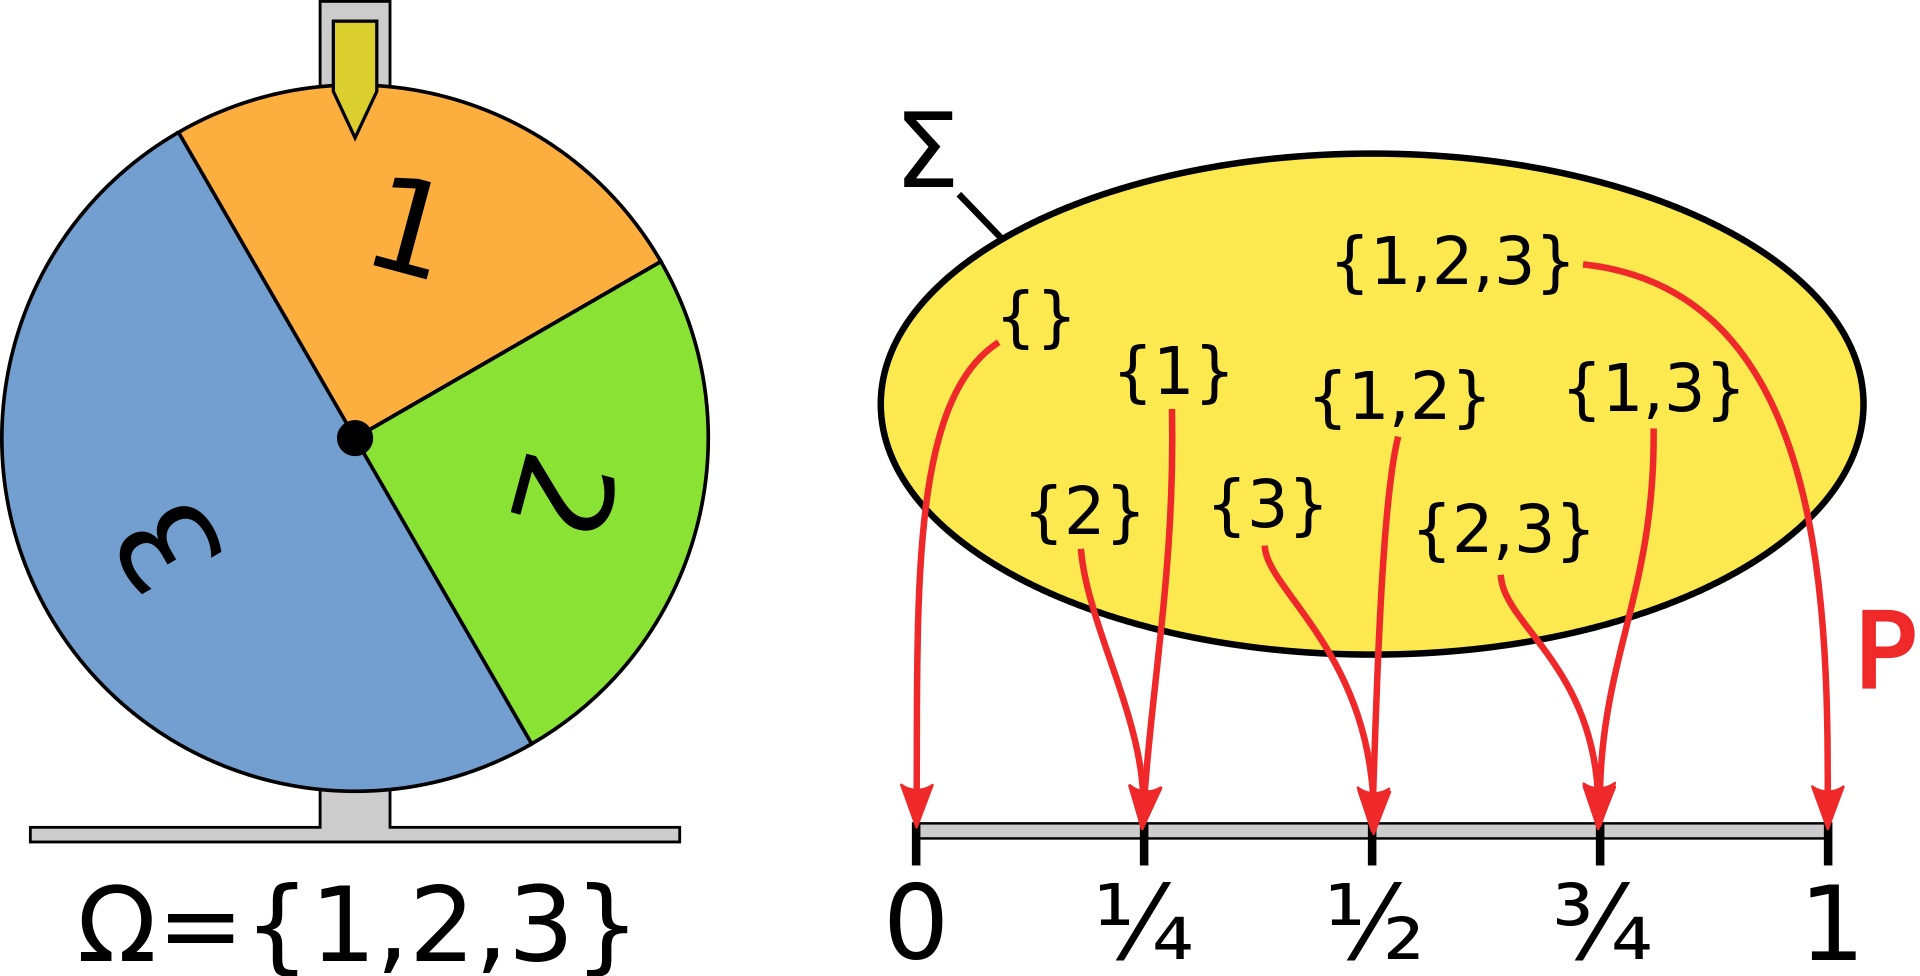
\includegraphics[width=53mm,height=\textheight,keepaspectratio]{images/Probability-measure.svg.png}

}

\caption{\label{fig-probability-space}Illustration of a probability
space by Ziggystar}

\end{marginfigure}%

\begin{tcolorbox}[enhanced jigsaw, bottomrule=.15mm, colbacktitle=quarto-callout-tip-color!10!white, leftrule=.75mm, bottomtitle=1mm, titlerule=0mm, title=\textcolor{quarto-callout-tip-color}{\faLightbulb}\hspace{0.5em}{Notation}, rightrule=.15mm, toprule=.15mm, colback=white, left=2mm, toptitle=1mm, arc=.35mm, opacitybacktitle=0.6, coltitle=black, breakable, opacityback=0, colframe=quarto-callout-tip-color-frame]

sometimes \(\mathcal{F}\) is replaced with \(\Sigma\). for the
\(\sigma\)-algebra like in the figure below

\end{tcolorbox}

\section{Properties of Probability
Measures}\label{sec-properties-of-probability-measures}

The probability of the \emph{null event} is 0.

\begin{equation}\phantomsection\label{eq-axiom-p1}{
\mathbb{P}r(\emptyset) = 0 
}\end{equation}

Probabilities of all possible events (the space of all possible
outcomes) must sum to one.

\begin{equation}\phantomsection\label{eq-axiom-p2}{ 
\mathbb{P}r(\Omega) = 1 
}\end{equation}

\begin{equation}\phantomsection\label{eq-axiom-p3}{
A\cap B = \emptyset \implies \mathbb{P}r(A \cup B) = \mathbb{P}r(A)+\mathbb{P}r(B) 
}\end{equation}

\phantomsection\label{trm-complements}
\begin{equation}\phantomsection\label{eq-complements}{
\mathbb{P}r(A^c) =1-\mathbb{P}r(A) \qquad \forall A\in\Omega 
}\end{equation}

if \(A\) is an event in \(\Omega\) then \(A^C\) is in Omega and since
they are mutually exclusive by Equation~\ref{eq-axiom-p2}

If \(S\) is the certain event in class \(C\) \(\Omega\) then

For every event \(X\) in class \(\Omega\)

\begin{equation}\phantomsection\label{eq-probability-axiom-1}{
1 \ge \mathbb{P}r(X) \ge 0 \qquad \forall X \in \Omega \qquad \text{(P1)} \qquad
}\end{equation}

Probabilities add to one:

\begin{equation}\phantomsection\label{eq-probability-axiom-2}{
\sum_{i\in \Omega} \mathbb{P}r(X=i)=1 \qquad \text{(P2)}\qquad
}\end{equation}

The complement of an event \(A\) is \(A^c\)

\begin{equation}\phantomsection\label{eq-probability-axiom-3}{
 \mathbb{P}r(S) = 1 
}\end{equation}

If events \(A_\lambda\) are mutually exclusive (only one event may
happen):

\begin{equation}\phantomsection\label{eq-probability-union-finite}{
\mathbb{P}r(A_1 \cup A_2) = \mathbb{P}r(A_1) + \mathbb{P}r(A_2) - \mathbb{P}r(A_1\cap A_1)
}\end{equation}

\begin{equation}\phantomsection\label{eq-probability-union}{
\mathbb{P}r(\bigcup_{\lambda\in \Omega} A_\lambda)=\sum_{\lambda \in \Omega} \mathbb{P}r(A_\lambda)
}\end{equation}

if \({B_i}\) is a finite or countably \emph{infinite partition} of a
sample space \(\Omega\) then

\begin{equation}\phantomsection\label{eq-law-of-total-probability}{
\mathbb{P}r(A) = {\sum_{i=1}^{N} \mathbb{P}r(A \cap B_i)}= {\sum_{i=1}^{N} \mathbb{P}r(A|B_i)\mathbb{P}r(B_i)}
}\end{equation}

\subsection{Odds}\label{sec-odds}

\begin{quote}
C-3PO: Sir, the possibility of successfully navigating an asteroid field
is approximately 3,720 to 1! Han Solo: Never tell me the odds! --- Star
Wars Episode V: The Empire Strikes Back
\end{quote}

Another way to think about probabilities is using \emph{odds}
Equation~\ref{eq-odds}. Odds are more intuitive when we are thinking
about the risk of an event happening or not happening. and when we
consider the risk associated with uncertainty odds are a handy way of
considering the risks.

\begin{definition}[Odds
Definitions]\protect\hypertarget{def-odds}{}\label{def-odds}

the odds of an event A are:

\begin{equation}\phantomsection\label{eq-odds}{
\mathcal{O}(A)  = \frac{\mathbb{P}r(A)}{\mathbb{P}r(A^c)} = \frac{ \mathbb{P}r(A)}{1-\mathbb{P}r(A)}
}\end{equation}

\end{definition}

It is also possible to convert odds to probabilities
Equation~\ref{eq-probability-from-odds}

\begin{theorem}[Probability from
odds]\protect\hypertarget{thm-probability-from-odds}{}\label{thm-probability-from-odds}

\begin{equation}\phantomsection\label{eq-probability-from-odds}{
\mathbb{P}r(A) = \frac{ \mathcal{O}(A)} {1+ \mathcal{O}(A)}
}\end{equation}

\end{theorem}

\begin{proof}
\[
\begin{aligned}
& & \mathcal{O}(A)  &= \frac{\mathbb{P}r(A)}{1-\mathbb{P}r(A)} && \text{(odds definition)} \\
   &\implies & \mathbb{P}r(A) &= \mathcal{O}(A) (1-\mathbb{P}r(A))  && (\times \text{ denominator}) \\
   &\implies &  \mathbb{P}r(A) &= \mathcal{O}(A) - \mathcal{O}(A) \mathbb{P}r(A) && \text{(expand)} \\
   &\implies &  \mathbb{P}r(A)(1+ \mathcal{O}(A)) &= \mathcal{O}(A) && \text{(collect)}   \\
   &\implies & \mathbb{P}r(A) &= \frac{ \mathcal{O}(A)} {1+ \mathcal{O}(A)} && \blacksquare  
\end{aligned}
\]
\end{proof}

If we are at the races and thinking about each horse a horse what we may
care about is if it will win or lose. In such a case the odds can
summarize the ratio of past successes and failures to win. Odds seem to
be in line with a frequentist view summarizing ratios of success to
failure. In reality, the other horses have odds as well and we may want
to consider the probability of winning given the other horses in the
race, and perhaps other parameters, like the track type, length of the
race, jockey, and perhaps some hot tips. So let us not get ahead of
ourselves

\begin{tcolorbox}[enhanced jigsaw, bottomrule=.15mm, colbacktitle=quarto-callout-tip-color!10!white, leftrule=.75mm, bottomtitle=1mm, titlerule=0mm, title=\textcolor{quarto-callout-tip-color}{\faLightbulb}\hspace{0.5em}{Data Scientist - insights.}, rightrule=.15mm, toprule=.15mm, colback=white, left=2mm, toptitle=1mm, arc=.35mm, opacitybacktitle=0.6, coltitle=black, breakable, opacityback=0, colframe=quarto-callout-tip-color-frame]

Many of these formulas are rather tedious. But, once you start to work
on a data science project you will often discover that there are some
problems with the data and because of that you cannot use your favorite
algorithm. Or worse when you do the results are not very useful. It is
at this point that the ability to think back to first principles will be
very fruitful. The more of this material you can recall, the more the
dots will connect, and your ability will translate into models of
increasing sophistication. Luckily, the rules of probability are
\emph{logical}. So it is fairly easy to remember or even derive if you
take some time to understand them.

I realize that figuring out which results are more useful is easier in
hindsight. And one of the reasons I am taking these courses is to
annotate in my note the results I think to be most useful.

\end{tcolorbox}

\subsection{Expectation}\label{sec-expectation}

The \emph{expectation} of a random variable (RV) X is the
\textbf{weighted average} of the outcomes it can take weighted by their
probabilities.

\begin{definition}[Expectation for a discrete
RV]\protect\hypertarget{def-expectation-discrete}{}\label{def-expectation-discrete}

\begin{equation}\phantomsection\label{eq-expectation-discrete}{
\mathbb{E}(x) = \sum^N_{i=1} x_i \times \mathbb{P}r(X=x_i)
}\end{equation}

\end{definition}

\begin{definition}[Expectation for a continuous
RV]\protect\hypertarget{def-expectation-continuous}{}\label{def-expectation-continuous}

\begin{equation}\phantomsection\label{eq-expectation-continuous}{
\mathbb{E}(x) = \int_{\Omega} x \mathbb{P}r(X=x) dx
}\end{equation}

\end{definition}

\section{Probability Paradigms}\label{sec-probability-paradigms}

\begin{marginfigure}

\centering{

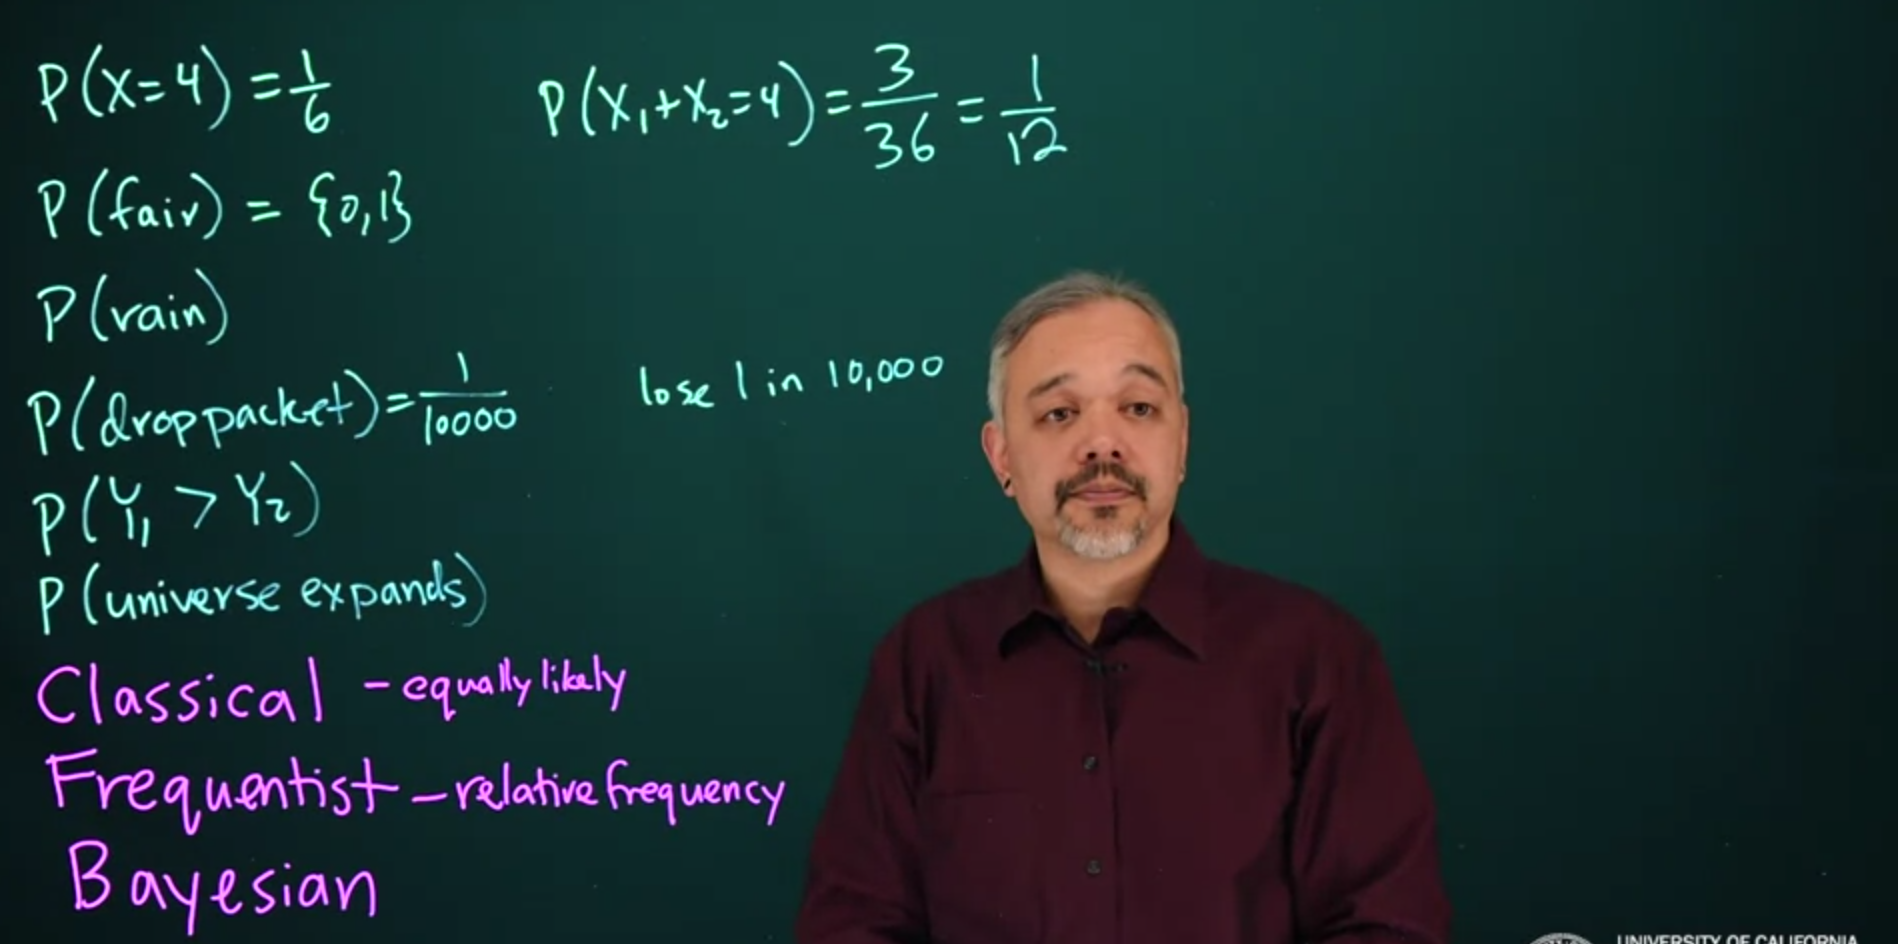
\includegraphics[width=53mm,height=\textheight,keepaspectratio]{images/c1l01-ss-01-paradigms.png}

}

\caption{\label{fig-prob-paradigms}Probability Paradigms}

\end{marginfigure}%

We start by looking at probability as defined or interpreted under three
paradigms. Probability is at its root a logical and scientific approach
to formalizing and modeling \emph{uncertainty}.

The three paradigms are:

\begin{definition}[Classical
Probability]\protect\hypertarget{def-classical}{}\label{def-classical}

Deals primarily with cases where probabilities are distributed equally,
like with dice and cards.

\end{definition}

\begin{marginfigure}

\centering{

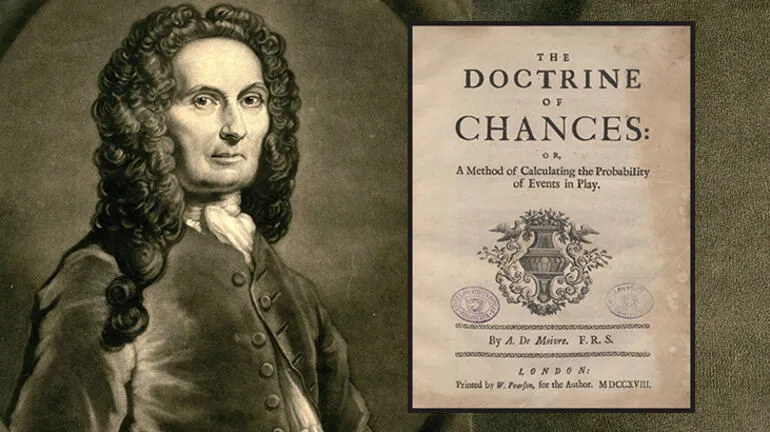
\includegraphics[width=53mm,height=\textheight,keepaspectratio]{images/bio-abraham-de-moivre-booked.png}

}

\caption{\label{fig-bio-abraham-de-moivre}Abraham De Moivre}

\end{marginfigure}%

\begin{tcolorbox}[enhanced jigsaw, bottomrule=.15mm, colbacktitle=quarto-callout-tip-color!10!white, leftrule=.75mm, bottomtitle=1mm, titlerule=0mm, title=\textcolor{quarto-callout-tip-color}{\faLightbulb}\hspace{0.5em}{Biographical note on Abraham de Moivre}, rightrule=.15mm, toprule=.15mm, colback=white, left=2mm, toptitle=1mm, arc=.35mm, opacitybacktitle=0.6, coltitle=black, breakable, opacityback=0, colframe=quarto-callout-tip-color-frame]

\begin{quote}
The Probability of an Event is greater or less, according to the number
of chances by which it may happen, compared with the whole number of
chances by which it may either happen or fail. --- (Moivre 1718)
\end{quote}

Abraham de Moivre (1667-1754) was a prominent French mathematician known
for his significant contributions to the field of probability and his
work on the foundations of Bayesian statistics. His research and
writings played a crucial role in establishing the mathematical
principles of probability theory and laid the groundwork for future
advancements in the field.

De Moivre is best known for his work on the theory of probability. He
made significant advancements in understanding the \emph{Binomial
distribution} and its application to games of chance and coin tossing.
In his influential book, ``The Doctrine of Chances'' (1718), he
presented a comprehensive treatise on probability theory, providing
mathematical explanations for various phenomena such as the law of large
numbers and the central limit theorem. His book became a standard
reference in the field and greatly influenced subsequent research on
probability.

Furthermore, de Moivre's work laid the foundation for Bayesian
statistics, although the term ``Bayesian'' was not coined until many
years after his death. He developed a formula known as de Moivre's
theorem, which establishes a connection between the normal distribution
and the binomial distribution. This theorem became a fundamental tool in
probability theory and enabled the calculation of probabilities for
large sample sizes. It provided a bridge between frequentist and
Bayesian approaches, allowing for the estimation of parameters and the
quantification of uncertainty.

\begin{quote}
And thus in all cases it will be found, that although Chance produces
irregularities, still the Odds will be infinitely great, that in process
of Time, those Irregularities will bear no proportion to the recurrency
of that Order which naturally results from Original Design. (Moivre
1718)
\end{quote}

He was an active participant in scientific societies and maintained
correspondence with renowned mathematicians of his time, including Isaac
Newton and James Stirling. His work played a crucial role in
disseminating mathematical knowledge and promoting the study of
probability theory across Europe. De Moivre's research and writings laid
the groundwork for the development of probability theory and Bayesian
statistics. His ideas and formulas continue to be foundational in the
field, and his contributions have had a lasting impact on mathematics,
statistics, and the broader scientific community.

His work remains an essential reference for researchers and serves as a
testament to his profound understanding of probability and statistics.

\begin{quote}
Further, the same Arguments which explode the Notion of Luck, may, on
the other side, be useful in some cases to establish a due comparison
between Chance and Design: We may imagine Chance and Design to be, as it
were, in Competition with each other, for the production of some sorts
of Events, and many calculate what Probability there is, that those
Events should be rather be owing to the one than to the other. (Moivre
1718)
\end{quote}

\end{tcolorbox}

\begin{definition}[Frequentist
Probability]\protect\hypertarget{def-frequentist}{}\label{def-frequentist}

Defines probabilities using long-run limits of frequencies from repeated
independent sampling generated by a hypothetical infinite sequence of
experiments from a population

\emph{Frequentist probability} or \emph{frequentism} is an
interpretation of probability; it defines an event's probability as the
limit of its relative frequency in many trials AKA \emph{long-run
probability}. Probabilities can be found, in principle, by a repeatable
objective process and are thus ideally devoid of opinion. The continued
use of frequentist methods in scientific inference, however, has been
called into question.

\begin{enumerate}
\def\labelenumi{\arabic{enumi}.}
\tightlist
\item
  Since in reality we cannot repeat most experiments many times.
\item
  ``by definition, scientific researchers do not possess sufficient
  knowledge about the relevant and irrelevant aspects of their tests and
  populations to be sure that their replications will be equivalent to
  one another'' - Mark Rubin 2020
\end{enumerate}

\end{definition}

\begin{definition}[Bayesian
Probability]\protect\hypertarget{def-bayesian}{}\label{def-bayesian}

Defines probability starting with a subjective view of the problem
called a prior and updates it as evidence comes in using Bayes Rule.

\end{definition}

The lesson and assignments test these views with examples - but the
division is rather artificial to me. Not that it does not exist, but
rather different authors on the subject treat it differently.

\section{Bayesian Probability and
Coherence}\label{sec-bayesian-probability-and-coherence}

\begin{marginfigure}

\centering{

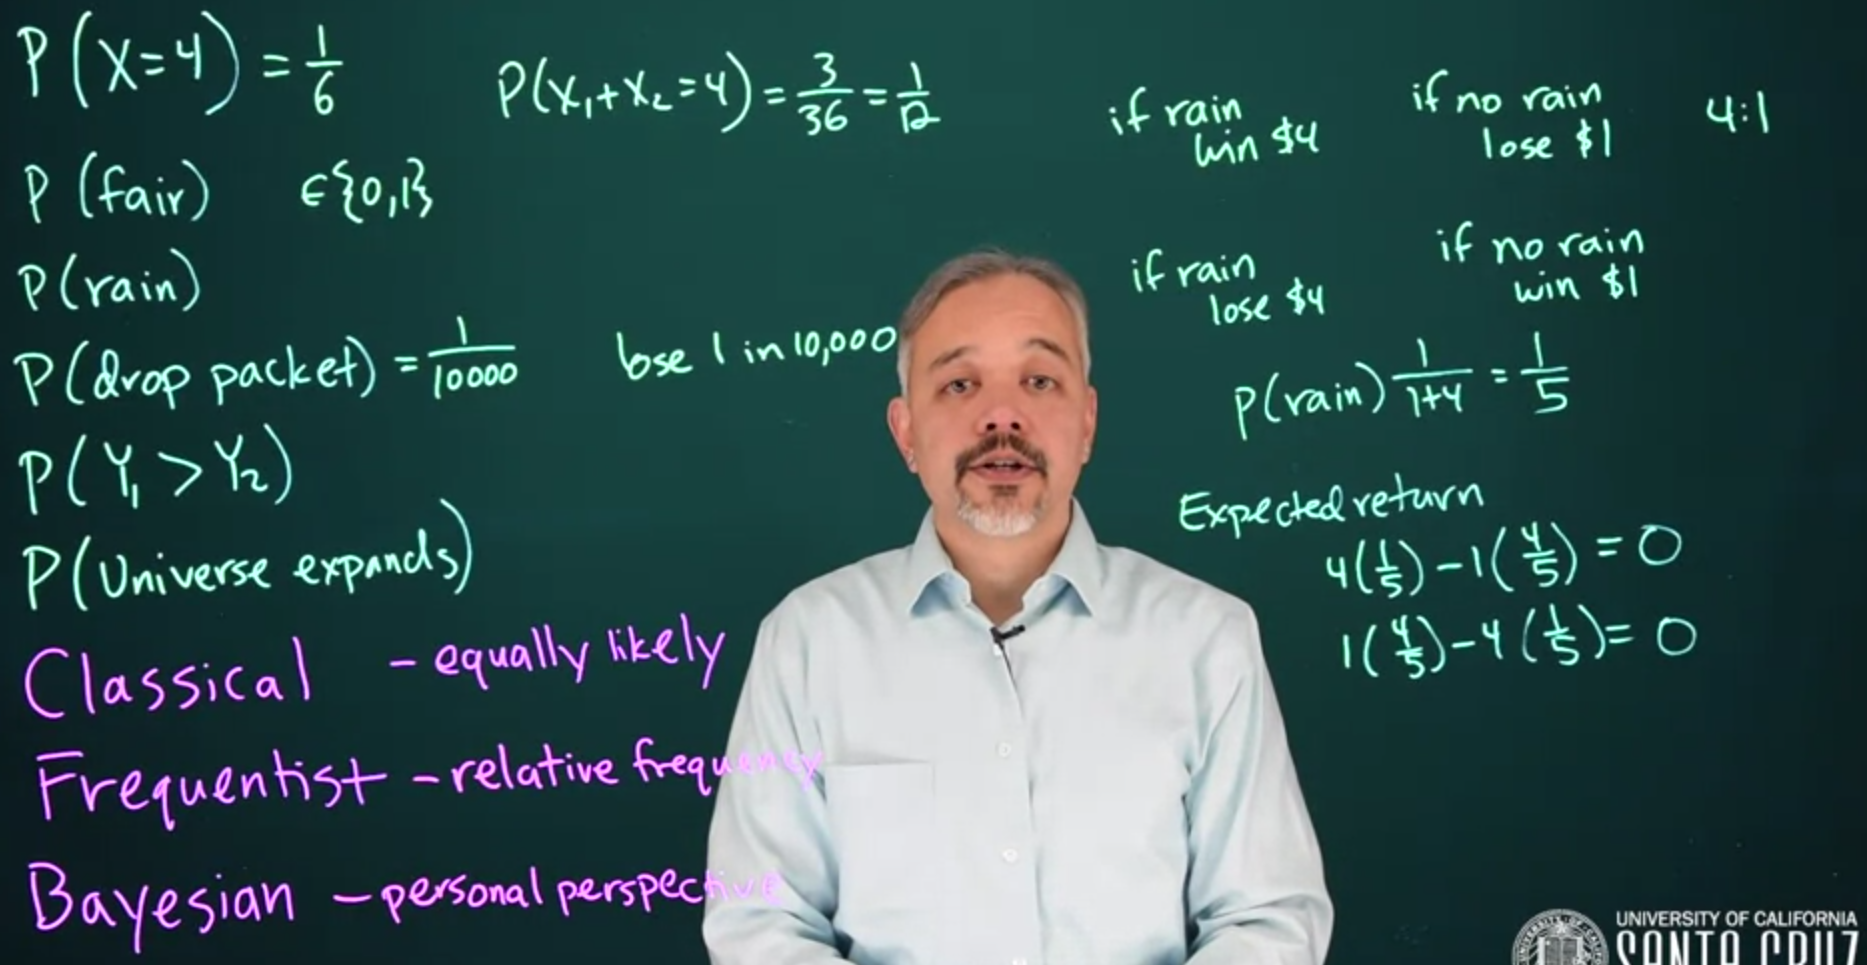
\includegraphics[width=53mm,height=\textheight,keepaspectratio]{images/c1l01-ss-02-coherence.png}

}

\caption{\label{fig-coherence}Coherence}

\end{marginfigure}%

A notion of a \textbf{fair bet} - one which we would take either way for
the same reward.

\begin{itemize}
\tightlist
\item
  \textbf{coherence} following the rules of statistics
\item
  \textbf{incoherence} or \textbf{Dutch book} one would be guaranteed to
  lose money.
\end{itemize}

\begin{marginfigure}

\centering{

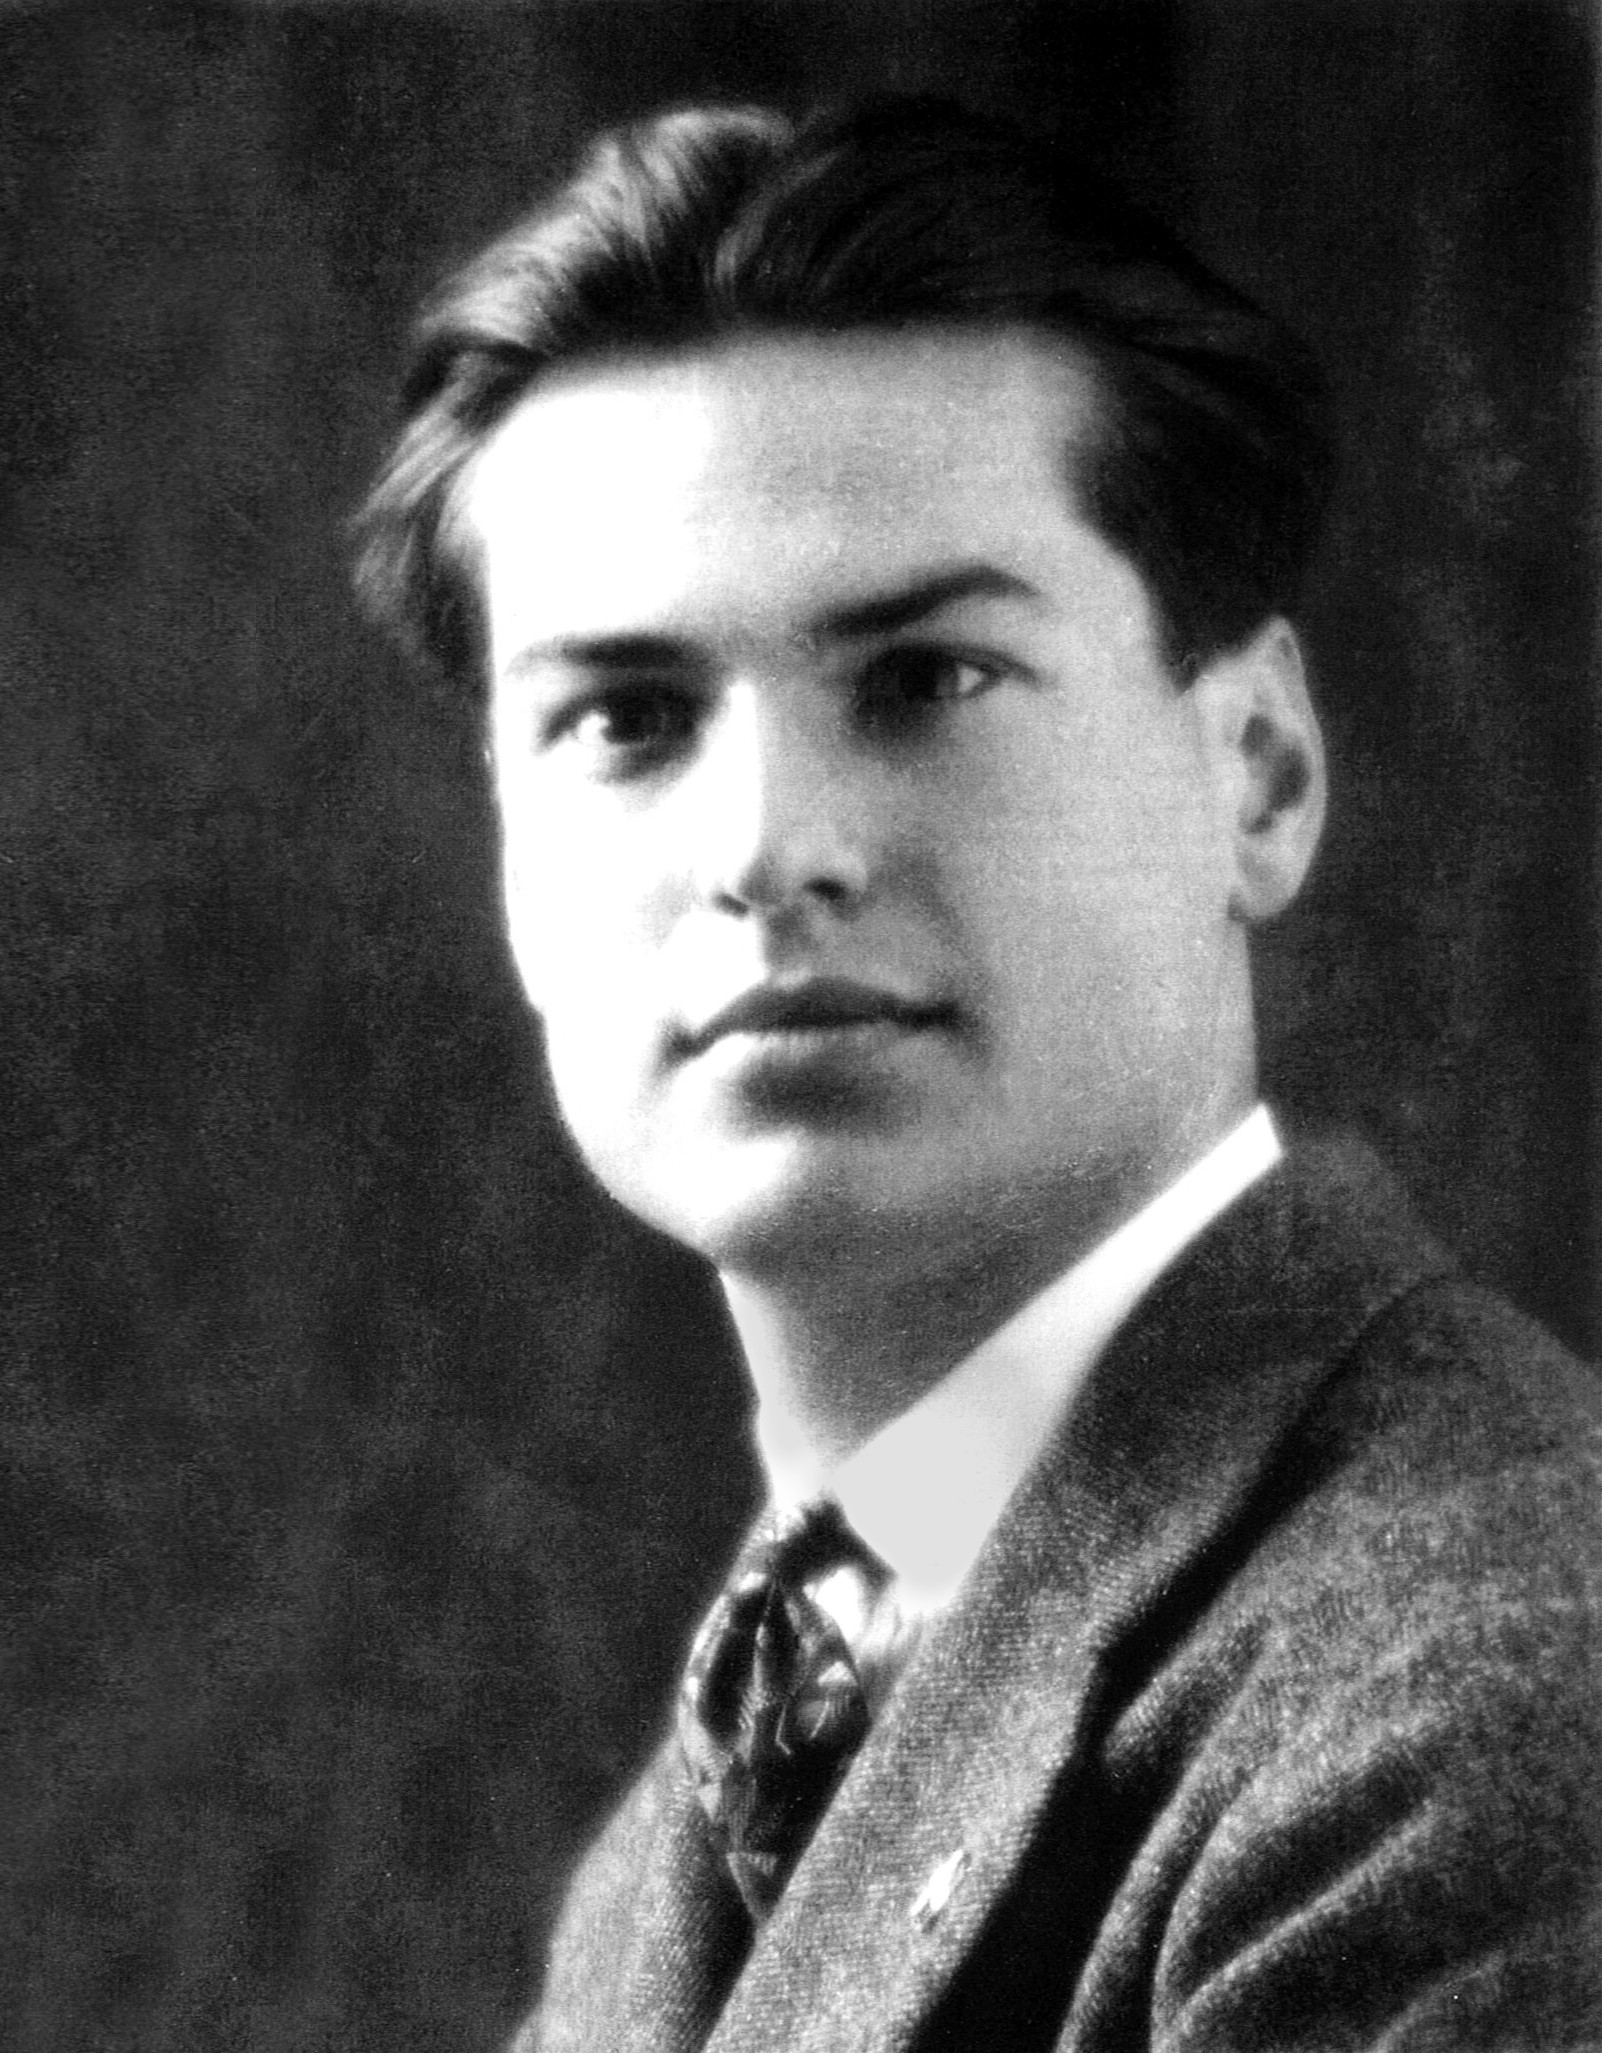
\includegraphics[width=53mm,height=\textheight,keepaspectratio]{images/bio-Bruno-de-Finetti.jpg}

}

\caption{\label{fig-bio-de-finetti}Bruno de Finetti}

\end{marginfigure}%

\begin{tcolorbox}[enhanced jigsaw, bottomrule=.15mm, colbacktitle=quarto-callout-tip-color!10!white, leftrule=.75mm, bottomtitle=1mm, titlerule=0mm, title=\textcolor{quarto-callout-tip-color}{\faLightbulb}\hspace{0.5em}{Biographical note on Bruno de Finetti}, rightrule=.15mm, toprule=.15mm, colback=white, left=2mm, toptitle=1mm, arc=.35mm, opacitybacktitle=0.6, coltitle=black, breakable, opacityback=0, colframe=quarto-callout-tip-color-frame]

\begin{quote}
From the subjective standpoint, no assertion is possible without a
priori opinion, but the variety of possible opinions makes problems
depending on different opinions interesting.
\end{quote}

Bruno de Finetti 1906-1985 was born in Innsbruck (Austria) to an Italian
family. He studied mathematics at the University of Trieste, where he
developed a keen interest in probability theory and its applications.

After completing his doctoral studies in 1928, de Finetti embarked on a
distinguished academic career. His first research work dealt with
mathematical biology and was published, in 1926 when he was still an
undergraduate. After graduation and up to 1931, he worked in the
mathematical office of the Central Italian Agency for Statistics. From
1931-46, de Finetti worked in Trieste at Assicurazioni Generali, one of
the most important insurance companies in Italy. In the same period, he
lectured at the University of Trieste and the University of Padua.

One of de Finetti's most significant contributions was his development
of the \textbf{theory of subjective probability}, also known as
\textbf{the Bayesian interpretation of probability}. He developed his
ideas independently of
\href{https://en.wikipedia.org/wiki/F._P._Ramsey}{F. P. Ramsey} who also
published on this (Ramsey 1926)

In his seminal work, (Finetti 1937), he proposed that probability should
be interpreted as a personal measure of belief or degree of uncertainty
rather than as a frequency or long-run proportion. This subjective
approach allowed for the incorporation of prior information and updating
of beliefs in light of new data, forming the basis of Bayesian
inference.

\begin{quote}
Probabilistic reasoning -- always to be understood as subjective --
merely stems from our being uncertain about something. (Finetti 2017 §
preface)
\end{quote}

It is impossible to summarize in a few paragraphs the scientific
activity of de Finetti in the different fields of mathematics
(probability), measure theory, analysis, geometry, mathematics of
finance, economics, the social sciences, teaching, computer science, and
biomathematics or to describe his generous and complex personality as a
scientist and a humanitarian. De Finetti discussed his own life in a
book edited by Gani (1982). See also the article by Lindley (1989).

\begin{quote}
My thesis, paradoxically, and a little provocatively, but nonetheless
genuinely, is simply this : \textbf{PROBABILITY DOES NOT EXIST}.
\ldots{} Probability, too, if regarded as something endowed with some
kind of objective existence, is no less a misleading misconception, an
illusory attempt to exteriorize or materialize our true probabilistic
beliefs. (Finetti 2017 § preface page x)
\end{quote}

de Finetti was a brilliant statistician but his books and papers have
garnered a reputation of being challenging to read both in the original
Italian, French and English translation. The above quote embodies his
radical point of view which he challenged other statisticians to rethink
their views.

What I think he meant is that meant primarily was that probabilities
unlike physical quantities cannot be measured in the objective sense. de
Fineti was well versed with quantum mechanics, where physical quantities
like the position and speed of an electron are interpreted primarily
through probabilities in a wave equation, to include a discussion in the
start of his second volume.

A large part of this course is that we are inferring parameters - which
are often probabilities.

Another milestone result by de Finetti is his theorem

\end{tcolorbox}

\begin{tcolorbox}[enhanced jigsaw, bottomrule=.15mm, colbacktitle=quarto-callout-note-color!10!white, leftrule=.75mm, bottomtitle=1mm, titlerule=0mm, title=\textcolor{quarto-callout-note-color}{\faInfo}\hspace{0.5em}{Question}, rightrule=.15mm, toprule=.15mm, colback=white, left=2mm, toptitle=1mm, arc=.35mm, opacitybacktitle=0.6, coltitle=black, breakable, opacityback=0, colframe=quarto-callout-note-color-frame]

Representing uncertainty with probability: \hl{Don't use any outside
information on this question, just determine probabilities
\emph{subjectively}}. The country of Chile is divided into 15
administrative regions. The size of the country is 756,096 square
kilometers. How big do you think the region of Atacama is? Let:

\begin{itemize}
\tightlist
\item
  \(A_1\) be the event: Atacama is less than 10,000 \(km^2\).
\item
  \(A_2\) be the event: Atacama is between 10,000 and 50,000 \(km^2\)
\item
  \(A_3\) be the event: Atacama is between 50,000 and 100,000 \(km^2\)
\item
  \(A_4\) be the event: Atacama is more than 100,000 \(km^2\) Assign
  probabilities to \(A_1 \ldots A_4\)
\end{itemize}

\marginnote{\begin{footnotesize}

\begin{longtable}[]{@{}llll@{}}
\toprule\noalign{}
Event & Min \(km^2\) & Max \(km^2\) & P \\
\midrule\noalign{}
\endhead
\bottomrule\noalign{}
\endlastfoot
\(A_1\) & 0 & 10k & \(\frac{1}{4}\) \\
\(A_2\) & 10k & 50k & \(\frac{1}{4}\) \\
\(A_3\) & 50k & 100k & \(\frac{1}{4}\) \\
\(A_4\) & 100k & & \(\frac{1}{4}\) \\
\end{longtable}

\end{footnotesize}}

\end{tcolorbox}

\begin{itemize}
\tightlist
\item
  What do I know at this point?

  \begin{itemize}
  \tightlist
  \item
    The expected area for the region is
    \(\frac{750,000}{15}=50,000\ km^2\) .
  \end{itemize}
\item
  What Do I believe?

  \begin{itemize}
  \tightlist
  \item
    I believe that the administrative regions have significantly
    different sizes
  \item
    from my familiarity with some other countries.
  \item
    As I don't know if Atacama is large or small my best \emph{bet} is
    to assign equal probabilities to each event.
  \end{itemize}
\end{itemize}

\begin{tcolorbox}[enhanced jigsaw, bottomrule=.15mm, colbacktitle=quarto-callout-note-color!10!white, leftrule=.75mm, bottomtitle=1mm, titlerule=0mm, title=\textcolor{quarto-callout-note-color}{\faInfo}\hspace{0.5em}{More information 1}, rightrule=.15mm, toprule=.15mm, colback=white, left=2mm, toptitle=1mm, arc=.35mm, opacitybacktitle=0.6, coltitle=black, breakable, opacityback=0, colframe=quarto-callout-note-color-frame]

Atacama is the fourth largest of 15 regions. Using this information, I
revised my probabilities as follows:

\marginnote{\begin{footnotesize}

\begin{longtable}[]{@{}llll@{}}
\toprule\noalign{}
Event & Min \(km^2\) & Max \(km^2\) & P \\
\midrule\noalign{}
\endhead
\bottomrule\noalign{}
\endlastfoot
\(A_1\) & & 10k & \(\frac{1}{16}\) \\
\(A_2\) & 10k & 50k & \(\frac{3}{16}\) \\
\(A_3\) & 50k & 100k & \(\frac{6}{16}\) \\
\(A_4\) & 100k & & \(\frac{6}{16}\) \\
\end{longtable}

\end{footnotesize}}

\end{tcolorbox}

\begin{itemize}
\tightlist
\item
  What do I know?

  \begin{itemize}
  \tightlist
  \item
    The expected area is \(\frac{750,000}{15}=50,000\ km^2\) .
  \item
    I know that Atacama is the Fourth largest.
  \end{itemize}
\item
  What Do I believe?

  \begin{itemize}
  \tightlist
  \item
    I believe that the administrative regions have significantly
    different sizes - from my familiarity with some other countries.
  \end{itemize}
\item
  How do I revise my guesstimate?

  \begin{itemize}
  \tightlist
  \item
    If the region sizes are equally sized I should gamble mostly on
    \(A_2\) and \(A_3\) .
  \item
    But I think there are a few large regions and many smaller ones.
  \item
    Also I know that 11 regions are smaller than Atacama and that 3
    three are larger.
  \item
    None of the events can yet be ruled out.
  \item
    \(A_1\) seems extremely unlikely as it necessitates the top three
    regions account for almost all of the area of the country.
    \(\frac{750,000 - 14 * 10,000}{3} = 203,333.3\) that's about 4 times
    the average for each state.
  \item
    \(A_2\) is fairly unlikely to require the top three regions to
    account for \(\frac{(750,000-14*20000)}{3}=170,000\) each that's
    more than 3 times the average.
  \end{itemize}
\end{itemize}

\begin{tcolorbox}[enhanced jigsaw, bottomrule=.15mm, colbacktitle=quarto-callout-note-color!10!white, leftrule=.75mm, bottomtitle=1mm, titlerule=0mm, title=\textcolor{quarto-callout-note-color}{\faInfo}\hspace{0.5em}{More information 2}, rightrule=.15mm, toprule=.15mm, colback=white, left=2mm, toptitle=1mm, arc=.35mm, opacitybacktitle=0.6, coltitle=black, breakable, opacityback=0, colframe=quarto-callout-note-color-frame]

The smallest region is the capital region, Santiago Metropolitan, which
has an area of 15,403 \(km^2\). Using this information, I revised my
probabilities as follows:

\marginnote{\begin{footnotesize}

\begin{longtable}[]{@{}llll@{}}
\toprule\noalign{}
Event & Min \(km^2\) & Max \(km^2\) & P \\
\midrule\noalign{}
\endhead
\bottomrule\noalign{}
\endlastfoot
\(A_1\) & & 10k & \(0\) \\
\(A_2\) & 10k & 50k & \(\frac{1}{8}\) \\
\(A_3\) & 50k & 100k & \(\frac{4}{8}\) \\
\(A_4\) & 100k & & \(\frac{3}{8}\) \\
\end{longtable}

\end{footnotesize}}

\end{tcolorbox}

What do I know?

\begin{itemize}
\tightlist
\item
  The expected area is \(\frac{750,000}{15}=50,000 \quad km^2\)
\item
  \(\mathbb{P}r(A_1)=0\) since the smallest region is \$ 15,403
  km\^{}2\$.
\item
  I believe that the administrative regions have significantly different
  sizes - from my familiarity with some other countries.
\item
  I know that Atacama is the Fourth largest.

  \begin{itemize}
  \tightlist
  \item
    If the region sizes are equally sized I should gamble mostly on
    \(A_2\) and \(A_3\).
  \item
    But I think there are a few large regions and many smaller ones.
  \item
    Also I know that 11 regions are smaller than Atacama and that 3
    three are larger.
  \item
    None of the events can yet be ruled out. But \(A1\) and \(A2\) are
    now very unlikely as they would require the top three regions to
    account for almost all of the area of the country.
  \end{itemize}
\end{itemize}

\begin{tcolorbox}[enhanced jigsaw, bottomrule=.15mm, colbacktitle=quarto-callout-note-color!10!white, leftrule=.75mm, bottomtitle=1mm, titlerule=0mm, title=\textcolor{quarto-callout-note-color}{\faInfo}\hspace{0.5em}{More information 3}, rightrule=.15mm, toprule=.15mm, colback=white, left=2mm, toptitle=1mm, arc=.35mm, opacitybacktitle=0.6, coltitle=black, breakable, opacityback=0, colframe=quarto-callout-note-color-frame]

The third largest region is Aysén del General Carlos Ibáñez del Campo,
which has an area of 108,494 \(km^2\).

Using this information, I revised my probabilities as follows:

\marginnote{\begin{footnotesize}

\begin{longtable}[]{@{}llll@{}}
\toprule\noalign{}
Event & Min \(km^2\) & Max \(km^2\) & P \\
\midrule\noalign{}
\endhead
\bottomrule\noalign{}
\endlastfoot
\(A_1\) & & 10K & \(0\) \\
\(A_2\) & 10k & 50K & \(\frac{1}{8}\) \\
\(A_3\) & 50k & 100K & \(\frac{6}{8}\) \\
\(A_4\) & 100k & & \(\frac{1}{8}\) \\
\end{longtable}

\end{footnotesize}}

\end{tcolorbox}

\begin{itemize}
\tightlist
\item
  The expected area is \(\frac{750,000}{15}=50,000 \quad km^2\)
\item
  \(\mathbb{P}r(A1)=0\) since the smallest region is \$15,403 km\^{}2 \$
  .
\item
  I believe that the administrative regions have significantly different
  sizes - from my familiarity with some other countries.
\item
  I know that Atacama is the Fourth largest.

  \begin{itemize}
  \tightlist
  \item
    If the region sizes are equally sized I should gamble mostly on
    \(A_2\) and \(A_3\) .
  \item
    But I think there are a few large regions and many smaller ones.
  \item
    Also I know that 11 regions are smaller than Atacama and that 3
    three are larger.
  \item
    None of the events can yet be ruled out. But A1 and A2 are now very
    unlikely as they would require the top three regions to account for
    almost all of the area of the country.
  \end{itemize}
\end{itemize}

\section{Discussions: Objectivity}\label{sec-discussions-objectivity}

\begin{tcolorbox}[enhanced jigsaw, bottomrule=.15mm, colbacktitle=quarto-callout-tip-color!10!white, leftrule=.75mm, bottomtitle=1mm, titlerule=0mm, title=\textcolor{quarto-callout-tip-color}{\faLightbulb}\hspace{0.5em}{Discussion: Objectivity}, rightrule=.15mm, toprule=.15mm, colback=white, left=2mm, toptitle=1mm, arc=.35mm, opacitybacktitle=0.6, coltitle=black, breakable, opacityback=0, colframe=quarto-callout-tip-color-frame]

In what ways could the frequentist paradigm be considered objective? In
what ways could the Bayesian paradigm be considered objective? Identify
ways in which each paradigm might be considered subjective.

\begin{itemize}
\tightlist
\item
  Frequentist:

  \begin{itemize}
  \tightlist
  \item
    The orthodox approach is statisticians should establish an objective
    statistical methodology and field researchers should then use it to
    solve their problems. This leads to following flow charts for
    analysis and tests without fully understanding the model and how it
    works. At best one makes mistakes due to misunderstanding. But we
    can see that there is a systematic gaming of this methodology using
    \emph{p-hacking}, \emph{multiple hypotheses}, and \emph{hiding
    failed experiments} leading to the publication of outrageously good
    results, which then cannot be replicated.
  \item
    The analysis is done on data that is supposedly sampled from a
    population. But the same data may belong to different populations
    (the city, the country, etc) each with different statistics. We
    should assume the same long-run frequencies would converge to
    different to each one of these statistics if we repeat the
    experiment enough times.
  \item
    The sample size, or how long we run the experiment is a tricky
    decision to make in advance and without prior knowledge. And if we
    do not decide in advance, but periodically as the data comes in. It
    turns out that this can completely change the outcomes of the
    experiment - even if both approaches have the same data.
  \item
    The choice of \(H_0\) and \(H_1\) is often subjective and each
    hypothesis can lead to yet another.
  \item
    The choice of the confidence level 95\%, 99\%, etc. used for
    statistical significance is subjective.
  \item
    If an effect size is considered large is subjective and depends on
    the field one studies.
  \end{itemize}
\item
  Bayesian:

  \begin{itemize}
  \tightlist
  \item
    the prior should be highly informative and therefore
    \textbf{subjective}. But it can be
  \item
    uninformative and hence more objective.
  \item
    it can be difficult to decide what impact the prior should have on
    the posterior. Ideally, we can quantify the effective sample size
    for the prior data and we can understand how much information each
    contributes to the posterior.
  \end{itemize}
\end{itemize}

\end{tcolorbox}

\section{Expected values}\label{sec-expected-values}

The \emph{expectation} of an RV is a measure of its central tendency.

The expected value, also known as the expectation or mean, of a random
variable \(X\) is denoted \(\mathbb{E}[X]\). It is the \emph{weighted
average} of all values \(X\) could take, weighted by their
probabilities.

\begin{tcolorbox}[enhanced jigsaw, bottomrule=.15mm, colbacktitle=quarto-callout-tip-color!10!white, leftrule=.75mm, bottomtitle=1mm, titlerule=0mm, title=\textcolor{quarto-callout-tip-color}{\faLightbulb}\hspace{0.5em}{Tip}, rightrule=.15mm, toprule=.15mm, colback=white, left=2mm, toptitle=1mm, arc=.35mm, opacitybacktitle=0.6, coltitle=black, breakable, opacityback=0, colframe=quarto-callout-tip-color-frame]

{\marginnote{\begin{footnotesize}\textbf{Why Square Brackets for
Expectation}\end{footnotesize}}}

I looked this up and found the following answer, see Autolatry (2015).

The RV X is a function whereas the Expectation is a Functional (a
mapping from a function to a number). Mathematicians adopt the use of
square brackets for functionals.

See Wikipedia contributors (2023b) for more information on what a
Functional is.

\end{tcolorbox}

\subsection{Expectation of a discrete random
variable}\label{expectation-of-a-discrete-random-variable}

If \(X\) is a discrete-valued random variable then its expectation is
defined by(\textbf{?@eq-expectation-discrete-RV})

\begin{equation}\phantomsection\label{eq-expectation-of-discrete-RV}{
\mathbb{E}[X]=\sum^N_{i=1} x_i \cdot \mathbb{P}r(X=x_i) = \sum^N_{i=1} x_i \cdot f(x) 
}\end{equation}

where \(f(x)\) is the probability mass function (PMF) of \(X\).

\subsection{Expectation of a continuous random
variable}\label{expectation-of-a-continuous-random-variable}

If \(X\) is a continuous random variable then its expectation is defined
by(\textbf{?@eq-expectation-continuous-RV})

\begin{equation}\phantomsection\label{eq-expectation-of-continuous-RV}{ 
\mathbb{E}[X]=\int_{-\infty}^{\infty} x \cdot f(x) dx
}\end{equation}

while the \emph{mean} is an important descriptive statistic for central
tendencies, we often prefer the \emph{median} which is robust to
outliers, and pick the \emph{mode} as a representative if we need a
value in the data set.

\subsection{Properties of Expectation}\label{properties-of-expectation}

Sum and integral are linear operators so the Expectation is also a
linear operator

\begin{equation}\phantomsection\label{eq-expectation-of-constant}{
\mathbb{E}[c]= c
}\end{equation}

\begin{equation}\phantomsection\label{eq-expectation-is-linear}{
\mathbb{E}[aX+bY] = a\mathbb{E}[X] + b\mathbb{E}[Y]
}\end{equation}

\begin{equation}\phantomsection\label{eq-expectation-of-function}{
\mathbb{E}[g[X]]  = \int{g(x)f(x)dx}
}\end{equation}

where \(g[X]\) is a function of the random variable \(X\).

If X \& Y are independent

\begin{equation}\phantomsection\label{eq-expectation-of-product-independent}{
\mathbb{E}[XY] = \mathbb{E}[X] \mathbb{E}[Y]
}\end{equation}

\section{Variance}\label{sec-variance}

\emph{Variance} is the dispersion of a distribution about the mean.

\begin{definition}[]\protect\hypertarget{def-variance-discrete}{}\label{def-variance-discrete}

For a discrete random variable, the Variance is defined using
(Equation~\ref{eq-variance-discrete})

\begin{equation}\phantomsection\label{eq-variance-discrete}{
\mathbb{V}ar(X)=\sum^N_{i=1} (x_i-\mu)^2 \mathbb{P}r(X=x_i)
}\end{equation}

\end{definition}

\begin{definition}[]\protect\hypertarget{def-variance-continuous}{}\label{def-variance-continuous}

For a continuous random variable, the Variance is defined using
(Equation~\ref{eq-variance-continuous})

\begin{equation}\phantomsection\label{eq-variance-continuous}{
\mathbb{V}ar[X]=\int_{- \infty}^{\infty} (x-\mu)^2 f(x)dx
}\end{equation}

\end{definition}

\subsection{Properties of Variance}\label{properties-of-variance}

\begin{equation}\phantomsection\label{eq-variance-of-constant}{
\mathbb{V}ar[c] = 0
}\end{equation}

if \(X\) and \(Y\) are independent then

\begin{equation}\phantomsection\label{eq-variance-is-linear}{
\mathbb{V}ar[aX+by] = a^2\mathbb{V}ar[X] +b^2\mathbb{V}ar[Y]
}\end{equation}

otherwise

\begin{equation}\phantomsection\label{eq-variance-is-linear-covariance}{
\mathbb{V}ar[aX+by] = a^2\mathbb{V}ar[X] +b^2\mathbb{V}ar[Y] + 2ab\mathbb{C}ov(X,Y)
}\end{equation}

where \(\mathbb{C}ov(X,Y)\) is the covariance of \(X\) and \(Y\).

Here is one of the most useful identities
(Equation~\ref{eq-variance-expectation}) for wrangling with variance
using the expectation of \(X\) and \(X^2\).

\begin{equation}\phantomsection\label{eq-variance-expectation}{
\begin{aligned}
    \mathbb{V}ar[X] &= \mathbb{E}[(X- \mathbb{E}[X])^2] 
    \\&= \mathbb{E}[X^2] − (\mathbb{E}[X])^2
\end{aligned}
}\end{equation}

\section{Covariance}\label{sec-covariance}

Covariance is a measure of the joint variability of two random
variables. It indicates the direction of the linear relationship between
the variables.

If \(X\) and \(Y\) are two random variables, the covariance of \(X\) and
\(Y\) is defined as:

\begin{equation}\phantomsection\label{eq-covariance}{
\begin{aligned}
\mathrm{Cov}(X,Y) &= \mathbb{E}[(X-\mathbb{E}[X])(Y-\mathbb{E}[Y])] 
\\ &= \mathbb{E}[XY]-\mathbb{E}[X]\mathbb{E}[Y]
\end{aligned}
}\end{equation}

\section{Correlation}\label{sec-correlation}

Correlation is a standardized measure of the linear relationship between
two random variables. It is a dimensionless quantity that ranges from -1
to 1.

The correlation coefficient \(\rho_{XY}\) is defined as the covariance
of \(X\) and \(Y\) divided by the product of their standard deviations:

\begin{equation}\phantomsection\label{eq-correlation}{
\rho_{XY} = \frac{\mathrm{Cov}(X,Y)}{\sigma_X\sigma_Y}
}\end{equation}

\chapter{Paradigms of probability -
M1L1HW1}\label{paradigms-of-probability---m1l1hw1}

Bayesian Statistics: From Concept to Data Analysis

\hfill\break

\begin{tcolorbox}[enhanced jigsaw, bottomrule=.15mm, colbacktitle=quarto-callout-caution-color!10!white, leftrule=.75mm, bottomtitle=1mm, titlerule=0mm, title=\textcolor{quarto-callout-caution-color}{\faFire}\hspace{0.5em}{Caution}, rightrule=.15mm, toprule=.15mm, colback=white, left=2mm, toptitle=1mm, arc=.35mm, opacitybacktitle=0.6, coltitle=black, breakable, opacityback=0, colframe=quarto-callout-caution-color-frame]

Section omitted to comply with the Honor Code

\end{tcolorbox}

\chapter{Bayes' Theorem - M1L2}\label{bayes-theorem---m1l2}

Bayesian Statistics: From Concept to Data Analysis

\hfill\break

\section{Bayes' Theorem}\label{sec-bayes-theorem}

\section{Conditional Probability}\label{sec-conditional-probability}

\begin{marginfigure}

\centering{

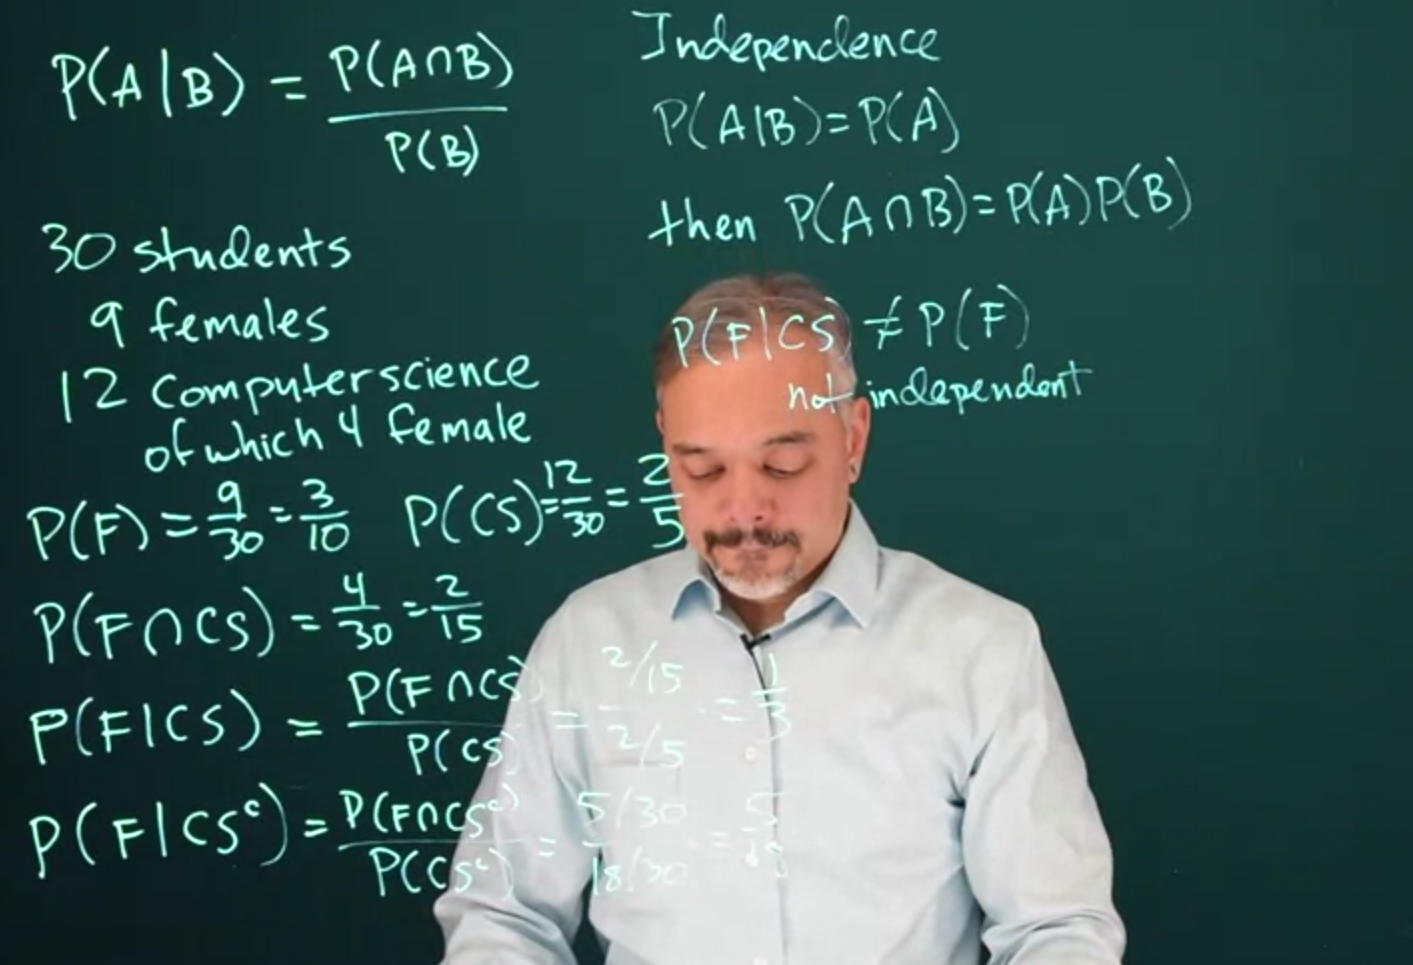
\includegraphics[width=53mm,height=\textheight,keepaspectratio]{images/c1l02-ss-01-conditional-probability.png}

}

\caption{\label{fig-conditional-probability}conditional probability}

\end{marginfigure}%

\begin{equation}\phantomsection\label{eq-conditional-probability}{
\mathbb{P}r(A \mid B)=\frac{\mathbb{P}r(A \cap B)}{\mathbb{P}r(B)}
}\end{equation}

independence

\begin{equation}\phantomsection\label{eq-conditional-independence}{
\mathbb{P}r(A \mid B) = \mathbb{P}r(A) \implies \mathbb{P}r(A \cap B) = \mathbb{P}r(A)\mathbb{P}r(B)
}\end{equation}

\subsection{Conditional Probability Example - Female CS
Student}\label{conditional-probability-example---female-cs-student}

Suppose there are 30 students, 9 of whom are female. Of the 30 students,
12 are computer science majors. 4 of those 12 computer science majors
are female. We want to estimate what is the probability of a student
being female given that she is a computer science major We start by
writing the above in the language of probability by converting
frequencies to probabilities. We start with the marginal. First, the
probability of a student being female from the data given above.

\[
\mathbb{P}r(\text{Female}) = \frac{9}{30} = \frac{3}{10}
\]

Next, we estimate the probability of a student being a computer science
major again just using the data given above.

\[
\mathbb{P}r(CS) = \frac{12}{30} = \frac{2}{5}
\]

Next, we can estimate the joint probability, i.e.~the probability of
being female and being a CS major. Again we have been given the numbers
in the data above.

\[
\mathbb{P}r(F\cap CS) = \frac{4}{30} = \frac{2}{15}
\]

Finally, we can use the definition of conditional probability and
substitute the above

\begin{equation}\phantomsection\label{eq-conditional-probability-example}{
\mathbb{P}r(F \mid CS) = \frac{\mathbb{P}r(F \cap CS)}{\mathbb{P}r(CS)} = \frac{2/15}{2/5} = \frac{1}{3}
}\end{equation}

An intuitive way to think about a conditional probability is that we're
looking at a sub-segment of the original population, and asking a
probability question within that segment

\begin{equation}\phantomsection\label{eq-conditional-probability-intuition}{
\mathbb{P}r(F \mid CS^c) = \frac{\mathbb{P}r(F\cap CS^c)}{ \mathbb{P}r (CS^c)} = \frac{5/30}{18/30} = \frac{5}{18}
}\end{equation}

The concept of \textbf{independence} is when one event does not depend
on another.

\[
A \perp \!\!\! \perp B \iff \mathbb{P}r(A \mid B) = \mathbb{P}r(A)
\]

It doesn't matter that B occurred.

If two events are independent then the following is true:

\begin{equation}\phantomsection\label{eq-def-independence}{
A \perp \!\!\! \perp B \iff \mathbb{P}r(A\cap B) = \mathbb{P}r(A)\mathbb{P}r(B) 
}\end{equation}

This can be derived from the conditional probability equation.

\subsection{Inverting Conditional
Probabilities}\label{inverting-conditional-probabilities}

If we don't know \(\mathbb{P}r(A \mid B)\) but we do know the inverse
probability \(\mathbb{P}r(B \mid A)\) is. We can then rewrite
\(\mathbb{P}r(A \mid B)\) in terms of \(\mathbb{P}r(B \mid A)\)

\begin{equation}\phantomsection\label{eq-bayes-rule}{
\mathbb{P}r(A \mid B) = \frac{\mathbb{P}r(B \mid A)\mathbb{P}r(A)}{\mathbb{P}r(B \mid A)\mathbb{P}r(A) + \mathbb{P}r(B \mid A^c)\mathbb{P}r(A^c)}
}\end{equation}

\subsection{Conditional Probability Example - ELISA HIV
test}\label{conditional-probability-example---elisa-hiv-test}

Let's look at an example of an early test for HIV antibodies known as
the ELISA test. - The test has a true positive rate of 0.977. - It has a
true negative rate of 0.926. - The incidence of HIV in North America is
.0026.

Now we want to know the probability of an individual having the disease
given that they tested positive \(\mathbb{P}r(HIV | +)\).

This is the inverse probability of the true positive, so we will need to
use Bayes' theorem.

We start by encoding the above using mathematical notation, so we know
what to substitute into Bayes' theorem.

The true positive rate is:

\[
\mathbb{P}r(+ \mid HIV) = 0.977
\]

The true negative rate is:

\[
\mathbb{P}r(- \mid NO\_HIV) = 0.926
\]

The probability of someone in North America having this disease was

\[
\mathbb{P}r(HIV) = .0026
\]

what we want is: \(\mathbb{P}r(HIV \mid +)\)

\begin{equation}\phantomsection\label{eq-bayes-hiv}{
\begin{aligned}
\mathbb{P}r(HIV \mid +) &= \frac{\mathbb{P}r(+ \mid HIV)\mathbb{P}r(HIV)}{\mathbb{P}r(+ \mid HIV)\mathbb{P}r(HIV) + \mathbb{P}r(+ \mid NO\_HIV){\mathbb{P}r(NO\_HIV)}}  \\ 
&= \frac{(.977)(.0026)}{(.977)(.0026) + (1-.977)(1-.0026)}  \\ 
&=  0.033 
\end{aligned}
}\end{equation}

This is a bit of a \textbf{surprise} - although the test has 90\% + true
and false accuracy - taking it once is only valid 3\% of the time. How
is this possible?

What happens in Bayes law is that we are updating probabilities. And
since we started with such a low probability of .0026, Bayesian updating
only brings it up to 0.03.

\begin{equation}\phantomsection\label{eq-bayes-law-multiple-events}{
\begin{aligned}
\mathbb{P}r(A \mid B) = \frac{\mathbb{P}r(B \mid A_1){(A_1)}}{\sum_{i=1}^{n}{\mathbb{P}r(B \mid A_i)}\mathbb{P}r(A_i)} \end{aligned}
}\end{equation}

Note: (McElreath (2015)) discusses how this can be presented less
surprisingly.

\section{Bayes' theorem 🎥}\label{sec-bayes-theorem-video}

\begin{marginfigure}

\centering{

\pandocbounded{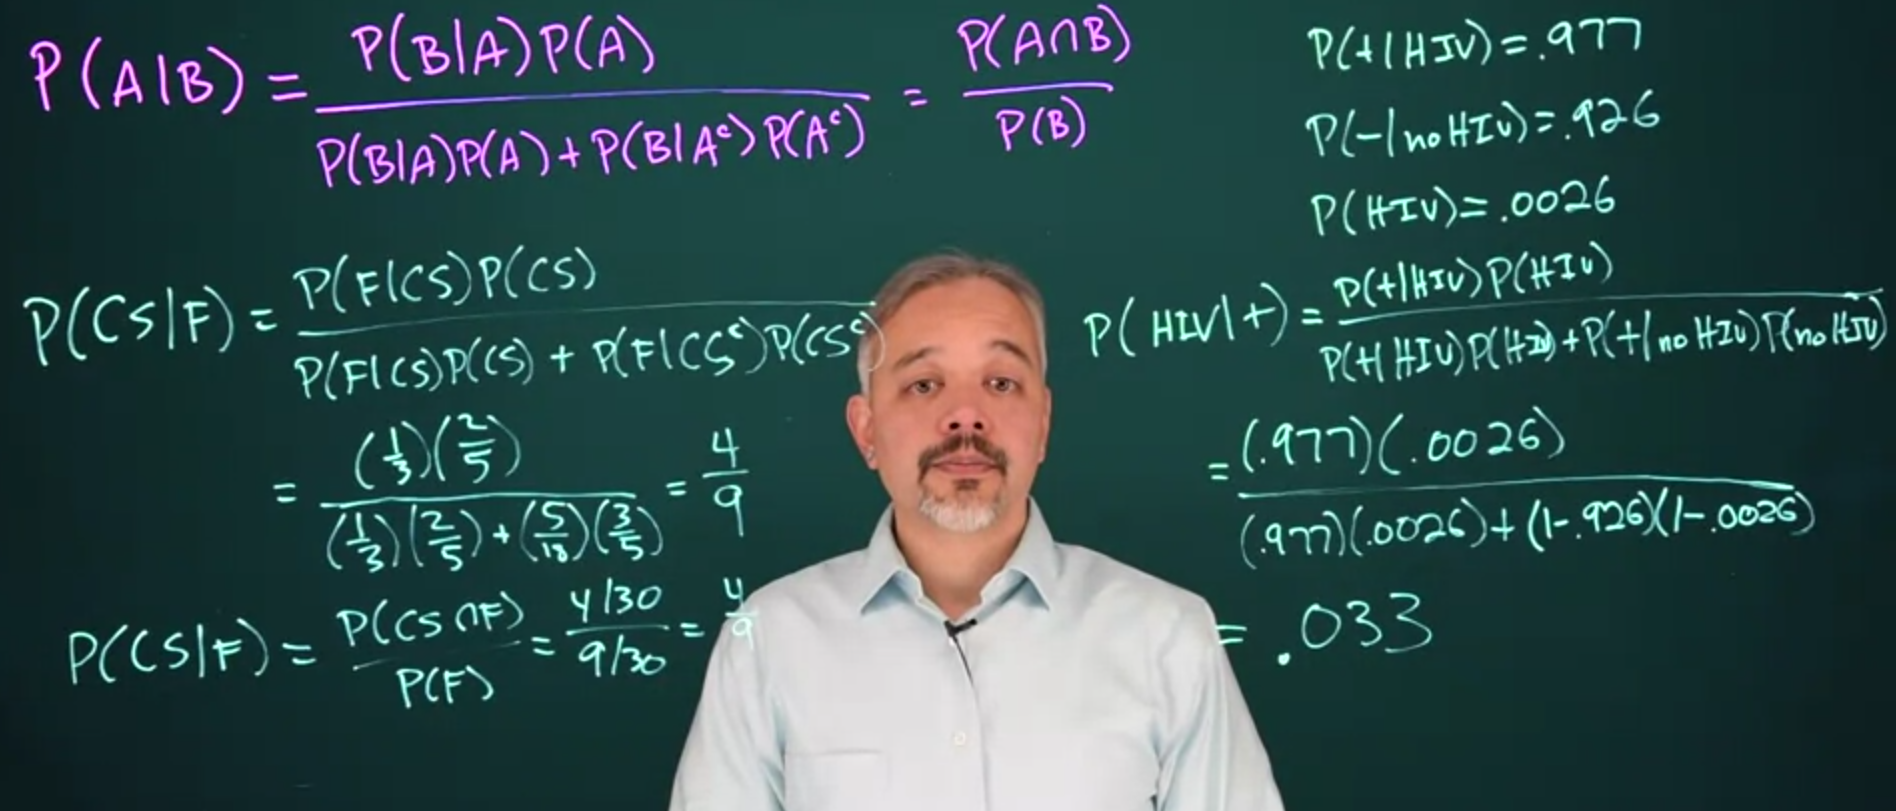
\includegraphics[keepaspectratio]{images/c1l01-ss-02-bayes-theorem.png}}

}

\caption{\label{fig-bayes-theorem}Bayes theorem}

\end{marginfigure}%

Here are a few formulations of Bayes' theorem. We denote \(H\) for our
hypothesis and \(E\) as our evidence i.e.~the data!

We start by using the definition of conditional probability:

\[
\mathbb{P}r(A \mid B) = \frac{ \mathbb{P}r(A \cap B)}{\mathbb{P}r(B)} \quad \text{(conditional probability)}
\]

\[
\begin{aligned}
{\color{orange} \overbrace{\color{orange} \mathbb{P}r(H|E)}^{\text{Posterior}}} &= \frac{  {\color{pink} \overbrace{\color{pink} \mathbb{P}r(H \cap E)}^{\text{Joint}}}  } {  {\color{green} \underbrace{{\color{green} \mathbb{P}r(\text{E})}}_{\text{Marginal Evidence}}} } \\ 
&= \frac{  {\color{red} \overbrace{\color{red} P (\text{H})}^{\text{Prior}}} \cdot  {\color{blue} \overbrace{\color{blue} P (E \mid H)}^{\text{Likelihood}}} } { {\color{green} \underbrace{{\color{green} \mathbb{P}r(E)}}_{\text{Marginal Evidence}}} } \\ 
&= \frac{  {\color{red} \overbrace{\color{red} P (H)}^{\text{Prior}}} \cdot {\color{blue} \overbrace{\color{blue} P (E \mid H)}^{\text{Likelihood}}} }{  {\color{green} \underbrace{\color{green} \mathbb{P}r(E \mid H) \mathbb{P}r(H) + \mathbb{P}r(E \mid H^c) \mathbb{P}r(H^c)  }_{\text{Marginal Evidence}}}}
\end{aligned}
\]

We can extend Bayes theorem to cases with multiple mutually exclusive
events:

\begin{marginfigure}

\centering{

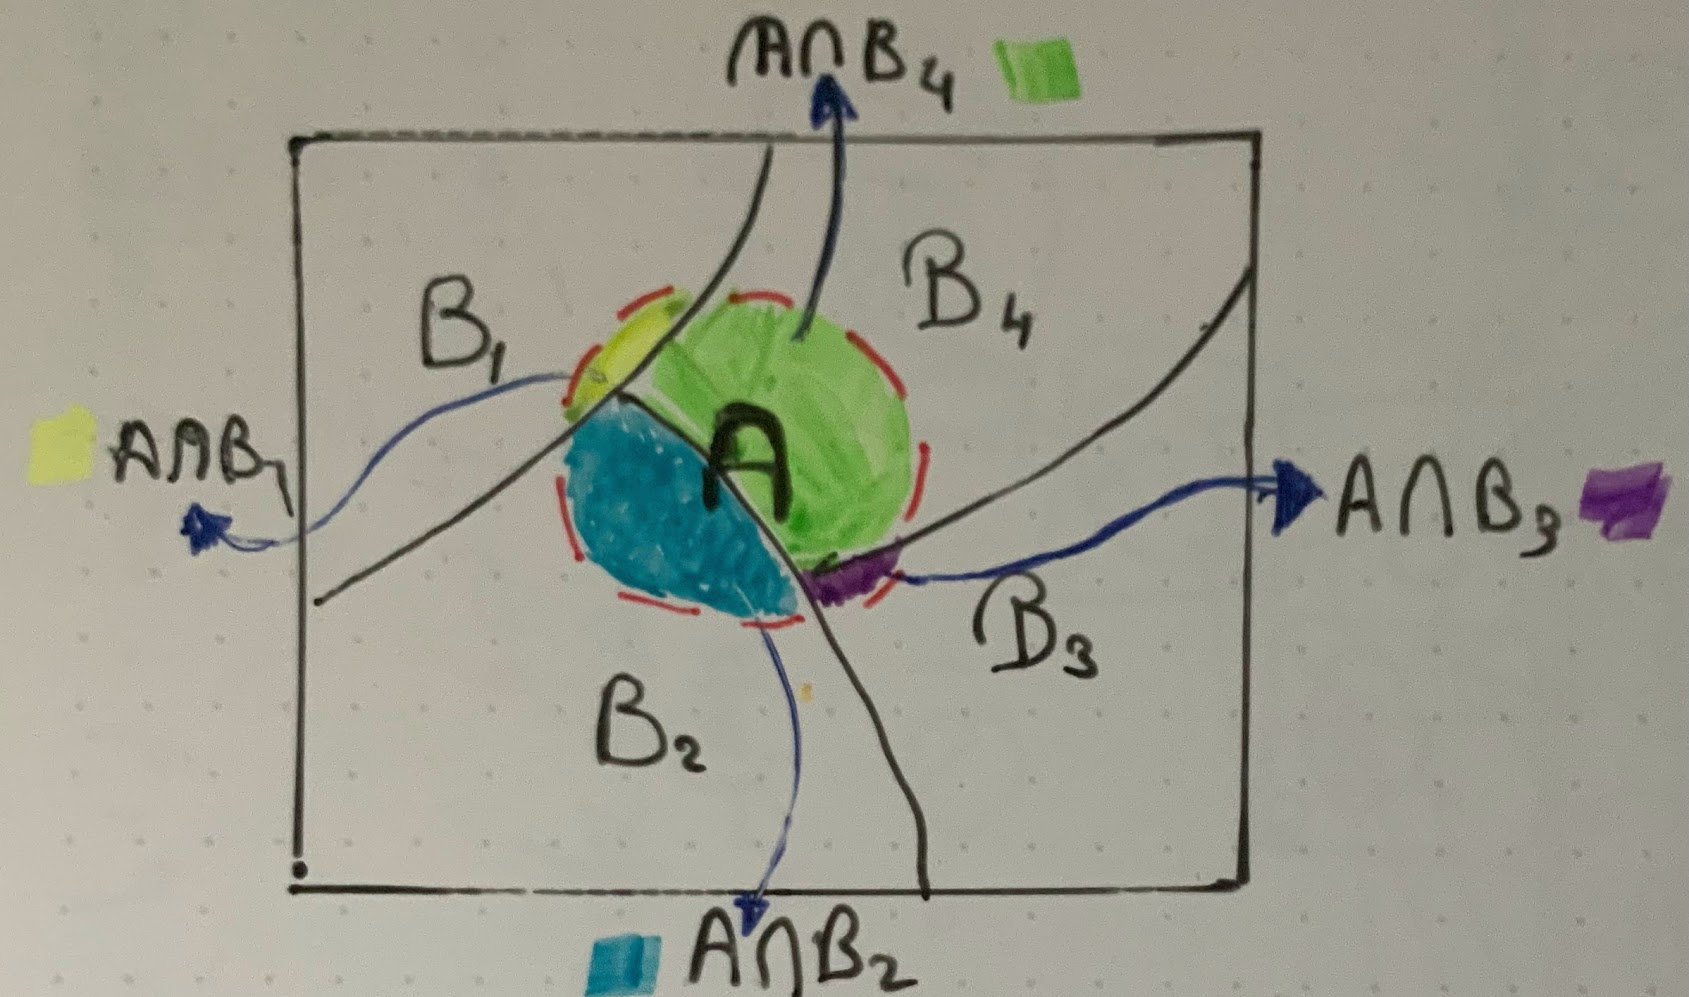
\includegraphics[width=53mm,height=\textheight,keepaspectratio]{images/total-probability.jpg}

}

\caption{\label{fig-mutually-exclusive-events}mutually exclusive events}

\end{marginfigure}%

if \(H_1 \ldots H_n\) are mutually exclusive events that sum to 1:

\[
\begin{aligned} \mathbb{P}r(H_1 \mid E) 
  & = \frac{\mathbb{P}r(E \mid H)\mathbb{P}r(H_1)}{\mathbb{P}r(E \mid H_1)\mathbb{P}r(H_1) +\ldots  + \mathbb{P}r(E \mid H_n)\mathbb{P}r(H_N)} \\ 
  & = \frac{\mathbb{P}r(E \mid H)\mathbb{P}r(H_1)}{\sum_{i=1}^{N} \mathbb{P}r(E \mid H_i)\mathbb{P}r(H_i)} \end{aligned}
\]

where we used the law of total probability in the denominator

if \(\{B_i\}\) is a finite or countably finite partition of a sample
space then

\[
\mathbb{P}r(A) = {\sum_{i=1}^{N} \mathbb{P}r(A \cup B_i)}= {\sum_{i=1}^{N} \mathbb{P}r(A \mid B_i)\mathbb{P}r(B_i)}
\]

\[
{\color{orange} P (\text{H} \mid \text{E})} = \frac {{\color{red} \mathbb{P}r(\text{H})} \times {\color{blue}\mathbb{P}r(\text{E} \mid \text{H})}} {\color{gray} {\mathbb{P}r(\text{E})}}
\]

\[
{\color{orange} \overbrace{\color{orange} P (\text{Unknown} \mid \text{Data})}^{\text{Posterior}}} = \frac {{\color{red} \overbrace{\color{red} P (\text{Unknown})}^{\text{Prior}}} \times {\color{blue} \overbrace{\color{blue} P (\text{Data} \mid \text{Unknown})}^{\text{Likelihood}}}} {{\color{green} \underbrace{{\color{green} \mathbb{P}r(\text{E})}}_{\text{Average likelihood}}}}
\]

The following is a video explaining Bayes law.

\section{Bayes' Theorem for continuous
distributions}\label{bayes-theorem-for-continuous-distributions}

When dealing with a continuous random variable \(\theta\), we can write
the conditional density for \(\theta\) given \(y\) as:

\begin{equation}\phantomsection\label{eq-bayes-continuous}{
f(\theta \mid y) =\frac{f(y\mid\theta)f(\theta)}{\int f(y\mid\theta) f(\theta) d\theta }
}\end{equation}

This expression does the same thing that the versions of Bayes' theorem
from Lesson 2 do. Because \(\theta\) is continuous, we integrate over
all possible values of \(\theta\) in the denominator rather than take
the sum over these values. The continuous version of Bayes' theorem will
play a central role from Lesson 5 on.

\begin{marginfigure}

\centering{

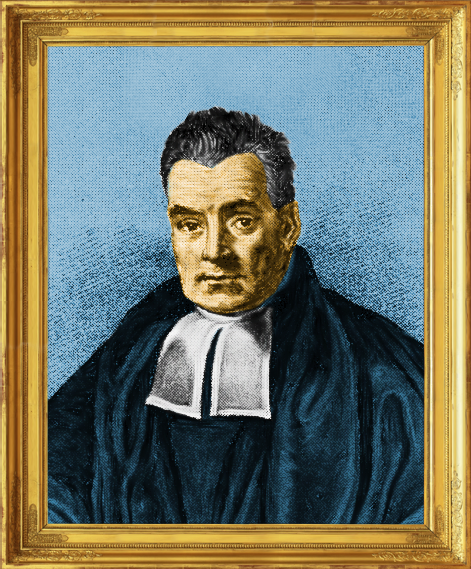
\includegraphics[width=53mm,height=\textheight,keepaspectratio]{images/bio-Thomas-Bayes.png}

}

\caption{\label{fig-bio-thomas-bayes}Rev.~Thomas Bayes by Mark Riehl}

\end{marginfigure}%

\begin{tcolorbox}[enhanced jigsaw, bottomrule=.15mm, colbacktitle=quarto-callout-tip-color!10!white, leftrule=.75mm, bottomtitle=1mm, titlerule=0mm, title=\textcolor{quarto-callout-tip-color}{\faLightbulb}\hspace{0.5em}{Historical Note on The Reverend Thomas Bayes}, rightrule=.15mm, toprule=.15mm, colback=white, left=2mm, toptitle=1mm, arc=.35mm, opacitybacktitle=0.6, coltitle=black, breakable, opacityback=0, colframe=quarto-callout-tip-color-frame]

Bayes Rule is due to Thomas Bayes (1701-1761) who was an English
statistician, philosopher and Presbyterian minister. Although Bayes
never published what would become his most famous accomplishment; his
notes were edited and published posthumously by Richard Price.

\end{tcolorbox}

\chapter{Conditional Probability and Bayes' Law -
M1L2HW1}\label{conditional-probability-and-bayes-law---m1l2hw1}

Bayesian Statistics: From Concept to Data Analysis

\hfill\break

\begin{tcolorbox}[enhanced jigsaw, bottomrule=.15mm, colbacktitle=quarto-callout-caution-color!10!white, leftrule=.75mm, bottomtitle=1mm, titlerule=0mm, title=\textcolor{quarto-callout-caution-color}{\faFire}\hspace{0.5em}{Caution}, rightrule=.15mm, toprule=.15mm, colback=white, left=2mm, toptitle=1mm, arc=.35mm, opacitybacktitle=0.6, coltitle=black, breakable, opacityback=0, colframe=quarto-callout-caution-color-frame]

Section omitted to comply with the Honor Code

\end{tcolorbox}

\chapter{Probability and Bayes' Theorem -
M1L2HW2}\label{probability-and-bayes-theorem---m1l2hw2}

Bayesian Statistics: From Concept to Data Analysis

\hfill\break

\begin{tcolorbox}[enhanced jigsaw, bottomrule=.15mm, colbacktitle=quarto-callout-caution-color!10!white, leftrule=.75mm, bottomtitle=1mm, titlerule=0mm, title=\textcolor{quarto-callout-caution-color}{\faFire}\hspace{0.5em}{Caution}, rightrule=.15mm, toprule=.15mm, colback=white, left=2mm, toptitle=1mm, arc=.35mm, opacitybacktitle=0.6, coltitle=black, breakable, opacityback=0, colframe=quarto-callout-caution-color-frame]

Section omitted to comply with the Honor Code

\end{tcolorbox}

\chapter{Distributions - M1L3}\label{distributions---m1l3}

Bayesian Statistics: From Concept to Data Analysis

\hfill\break

\section{Distributions}\label{sec-distributions}

\section{The Bernoulli \& Binomial
Distribution}\label{sec-the-bernoulli--binomial-distribution}

\begin{marginfigure}

\centering{

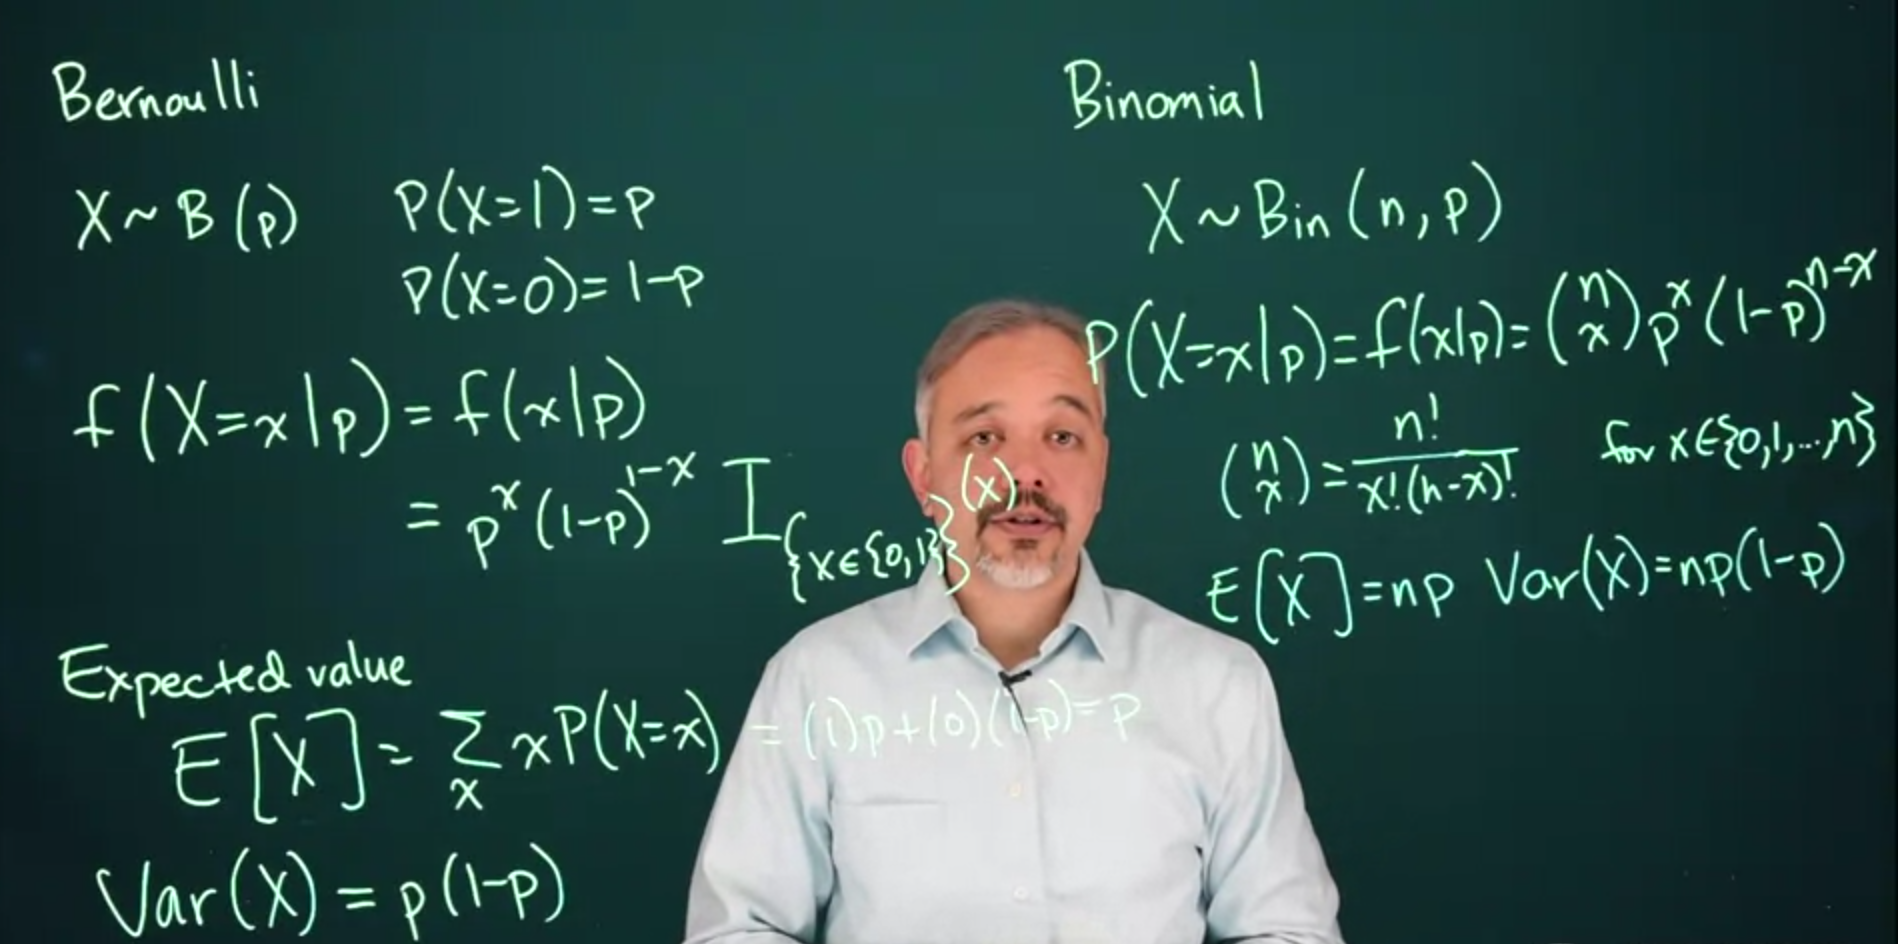
\includegraphics[width=53mm,height=\textheight,keepaspectratio]{images/c1l03-ss-01-bernoulli-and-binomial-distributions.png}

}

\caption{\label{fig-slide-l03-s01}Bernoulli and Binomial Distributions}

\end{marginfigure}%

These two distributions are built on a trial of a coin toss (possibly
biased).

\begin{itemize}
\tightlist
\item
  We use the Bernoulli distribution to model a random variable for the
  probability of such a coin toss trial.
\item
  We use the Binomial distribution to model a random variable for the
  probability of getting \(k\) heads in \(N\) independent trials.
\end{itemize}

\subsection{The Bernoulli
Distribution}\label{sec-the-bernoulli-distribution}

Arises when modeling events with two possible outcomes, \textbf{Success}
and \textbf{Failure} for a coin toss these can be \textbf{Heads} and
\textbf{Tails}

\begin{equation}\phantomsection\label{eq-l3-bernoulli-rv}{
X \sim \mathrm{Bernoulli}(p) = 
\begin{cases} 
   \mathbb{P}r(X=1) = p & \text{success} \\
   \mathbb{P}r(X=0)=1-p & \text{failure}
\end{cases}
}\end{equation}

Where parameter p is the probability of getting heads.

The probability for the two events is:

Notation:

\begin{itemize}
\tightlist
\item
  we use (Roman) p if its value is known.\\
\item
  we use (Greek) \(\theta\) when its value is unknown.
\end{itemize}

This is a probability mass function since it is discrete. But we call it
a Probability Density Function (PDF) in the measure-theoretic sense.

\begin{equation}\phantomsection\label{eq-l3-bernoulli-pmf}{
f(X=x\mid p) = p^x(1-p)^x \mathbb{I}_{[0,1]}(x)
}\end{equation}

\begin{equation}\phantomsection\label{eq-l3-bernoulli-expectation}{
\mathbb{E}(x)= p 
}\end{equation}

\begin{equation}\phantomsection\label{eq-l3-bernoulli-variance}{
\text{Var}(x)= \mathbb{P}r(1-p)
}\end{equation}

\begin{Shaded}
\begin{Highlighting}[]
\ImportTok{import}\NormalTok{ numpy }\ImportTok{as}\NormalTok{ np}
\ImportTok{from}\NormalTok{ scipy.stats }\ImportTok{import}\NormalTok{ bernoulli}
\ImportTok{import}\NormalTok{ matplotlib.pyplot }\ImportTok{as}\NormalTok{ plt}

\NormalTok{fig, ax }\OperatorTok{=}\NormalTok{ plt.subplots(}\DecValTok{1}\NormalTok{, }\DecValTok{1}\NormalTok{)}
\NormalTok{p }\OperatorTok{=} \FloatTok{0.3}
\NormalTok{mean, var, skew, kurt }\OperatorTok{=}\NormalTok{ bernoulli.stats(p, moments}\OperatorTok{=}\StringTok{\textquotesingle{}mvsk\textquotesingle{}}\NormalTok{)}
\BuiltInTok{print}\NormalTok{(}\SpecialStringTok{f\textquotesingle{}}\SpecialCharTok{\{}\NormalTok{mean}\OperatorTok{=}\SpecialCharTok{:1.2f\}}\SpecialStringTok{, }\SpecialCharTok{\{}\NormalTok{var}\OperatorTok{=}\SpecialCharTok{:1.2f\}}\SpecialStringTok{, }\SpecialCharTok{\{}\NormalTok{skew}\OperatorTok{=}\SpecialCharTok{:1.2f\}}\SpecialStringTok{, }\SpecialCharTok{\{}\NormalTok{kurt}\OperatorTok{=}\SpecialCharTok{:1.2f\}}\SpecialStringTok{\textquotesingle{}}\NormalTok{)}
\end{Highlighting}
\end{Shaded}

\begin{verbatim}
mean=0.30, var=0.21, skew=0.87, kurt=-1.24
\end{verbatim}

\begin{Shaded}
\begin{Highlighting}[]
\NormalTok{x }\OperatorTok{=}\NormalTok{ np.arange(bernoulli.ppf(}\FloatTok{0.01}\NormalTok{, p),}
\NormalTok{              bernoulli.ppf(}\FloatTok{0.99}\NormalTok{, p))}
\NormalTok{ax.plot(x, bernoulli.pmf(x, p), }\StringTok{\textquotesingle{}bo\textquotesingle{}}\NormalTok{, ms}\OperatorTok{=}\DecValTok{8}\NormalTok{, label}\OperatorTok{=}\StringTok{\textquotesingle{}bernoulli pmf\textquotesingle{}}\NormalTok{)}
\NormalTok{ax.vlines(x, }\DecValTok{0}\NormalTok{, bernoulli.pmf(x, p), colors}\OperatorTok{=}\StringTok{\textquotesingle{}b\textquotesingle{}}\NormalTok{, lw}\OperatorTok{=}\DecValTok{5}\NormalTok{, alpha}\OperatorTok{=}\FloatTok{0.5}\NormalTok{)}

\NormalTok{rv }\OperatorTok{=}\NormalTok{ bernoulli(p)}
\NormalTok{ax.vlines(x, }\DecValTok{0}\NormalTok{, rv.pmf(x), colors}\OperatorTok{=}\StringTok{\textquotesingle{}k\textquotesingle{}}\NormalTok{, linestyles}\OperatorTok{=}\StringTok{\textquotesingle{}{-}\textquotesingle{}}\NormalTok{, lw}\OperatorTok{=}\DecValTok{1}\NormalTok{,}
\NormalTok{        label}\OperatorTok{=}\StringTok{\textquotesingle{}frozen pmf\textquotesingle{}}\NormalTok{)}
\NormalTok{ax.legend(loc}\OperatorTok{=}\StringTok{\textquotesingle{}best\textquotesingle{}}\NormalTok{, frameon}\OperatorTok{=}\VariableTok{False}\NormalTok{)}
\NormalTok{plt.show()}
\end{Highlighting}
\end{Shaded}

\begin{figure}[H]

{\centering \pandocbounded{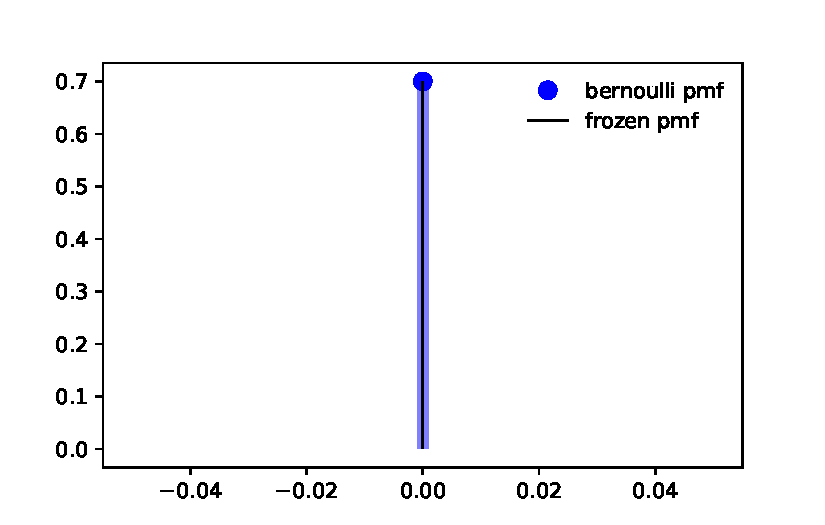
\includegraphics[keepaspectratio]{C1-L03_files/figure-pdf/bernoulli-distribution-1.pdf}}

}

\caption{Bernoulli distribution}

\end{figure}%

\begin{Shaded}
\begin{Highlighting}[]
\CommentTok{\#\# Generate random numbers}
\NormalTok{r }\OperatorTok{=}\NormalTok{ bernoulli.rvs(p, size}\OperatorTok{=}\DecValTok{10}\NormalTok{)}
\NormalTok{r}
\end{Highlighting}
\end{Shaded}

\begin{verbatim}
array([0, 1, 1, 0, 0, 0, 1, 0, 0, 1])
\end{verbatim}

\begin{marginfigure}

\centering{

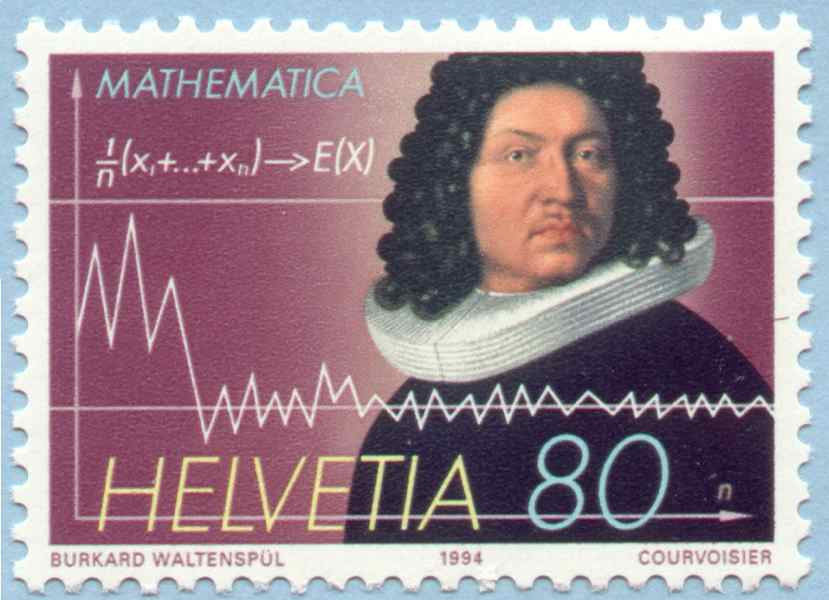
\includegraphics[width=53mm,height=\textheight,keepaspectratio]{images/bio-bernoulli.jpg}

}

\caption{\label{fig-bio-bernoulli}Jacob Bernoulli}

\end{marginfigure}%

\begin{tcolorbox}[enhanced jigsaw, bottomrule=.15mm, colbacktitle=quarto-callout-tip-color!10!white, leftrule=.75mm, bottomtitle=1mm, titlerule=0mm, title=\textcolor{quarto-callout-tip-color}{\faLightbulb}\hspace{0.5em}{Biographical note on Jacob Bernoulli}, rightrule=.15mm, toprule=.15mm, colback=white, left=2mm, toptitle=1mm, arc=.35mm, opacitybacktitle=0.6, coltitle=black, breakable, opacityback=0, colframe=quarto-callout-tip-color-frame]

\begin{quote}
It seems that to make a correct conjecture about any event whatever, it
is necessary to calculate exactly the number of possible cases and then
to determine how much more likely it is that one case will occur than
another. (Bernoulli 1713)
\end{quote}

The Bernoulli distribution as well as The Binomial distribution are due
to Jacob Bernoulli (1655-1705) who was a prominent mathematicians in the
Bernoulli family. He discovered the fundamental mathematical constant e.
However, his most important contribution was in the field of
probability, where he derived the first version of the law of large
numbers.

for a fuller
\href{https://mathshistory.st-andrews.ac.uk/Biographies/Bernoulli_Jacob/}{biography
see}

\end{tcolorbox}

\subsection{The Binomial Distribution}\label{the-binomial-distribution}

\begin{equation}\phantomsection\label{eq-l3-bernoulli-experiment}{
\overbrace{\underbrace{\fbox{0}\ \ldots \fbox{0}}_{N_0}\ \underbrace{\fbox{1}\ \ldots \fbox{1}}_{N_1}}^N 
}\end{equation}

The Binomial distribution models \texttt{counts} of successes in
independent Bernoulli trials \index{Bernoulli trial}. It arises when we
need to consider the summing N independent and identically distributed
Bernoulli RV with the same probability of success \(\theta\).

\begin{tcolorbox}[enhanced jigsaw, bottomrule=.15mm, colbacktitle=quarto-callout-tip-color!10!white, leftrule=.75mm, bottomtitle=1mm, titlerule=0mm, title=\textcolor{quarto-callout-tip-color}{\faLightbulb}\hspace{0.5em}{Conditions}, rightrule=.15mm, toprule=.15mm, colback=white, left=2mm, toptitle=1mm, arc=.35mm, opacitybacktitle=0.6, coltitle=black, breakable, opacityback=0, colframe=quarto-callout-tip-color-frame]

\begin{itemize}
\tightlist
\item
  Discrete data
\item
  Two possible outcomes for each trial
\item
  Each trial is independent
\item
  The probability of success/failure is the same in each trial
\end{itemize}

\end{tcolorbox}

\begin{figure}[H]

{\centering 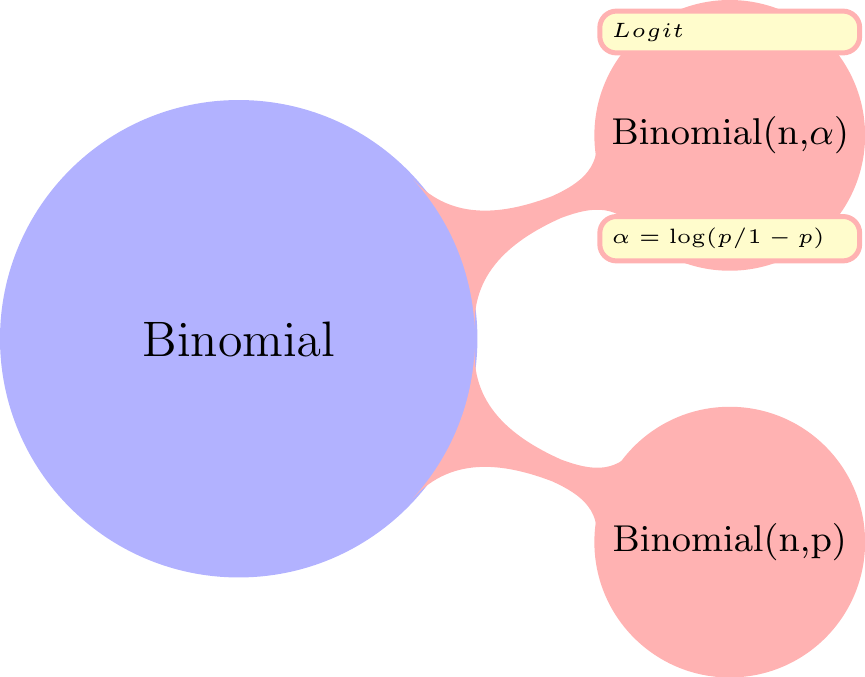
\includegraphics[width=1\linewidth,height=\textheight,keepaspectratio]{C1-L03_files/figure-pdf/Binomial-reparams-1.png}

}

\caption{Binomial reparams mindmap}

\end{figure}%

\begin{equation}\phantomsection\label{eq-l3-binomial-rv}{
X \sim \mathrm{Bin}(n,p)
}\end{equation}

the probability function

\begin{equation}\phantomsection\label{eq-l3-binomial-pmf}{
f(X=x \mid \theta) = {n \choose x} \theta^x(1-\theta)^{n-x}
}\end{equation}

\begin{equation}\phantomsection\label{eq-l3-binomial-likelihood}{
\mathcal{L}(\theta)=\prod_{i=1}^{n} {n\choose x_i}  \theta ^ {x_i} (1− \theta) ^ {(n−x_i)}
}\end{equation}

\begin{equation}\phantomsection\label{eq-l3-binomial-log-likelihood}{
\begin{aligned}
\ell( \theta) &= \log \mathcal{L}( \theta) \\
              &= \sum_{i=1}^n \left[\log {n\choose x_i} + x_i \log  \theta + (n-x_i)\log (1- \theta) \right]
\end{aligned}
}\end{equation}

\begin{equation}\phantomsection\label{eq-l3-binomial-expectation}{
\mathbb{E}[X]= N \times  \theta 
}\end{equation}

\begin{equation}\phantomsection\label{eq-l3-binomial-variance}{
\mathbb{V}ar[X]=N \cdot \theta \cdot (1-\theta)
}\end{equation}

\begin{equation}\phantomsection\label{eq-l3-binomial-entropy}{
\mathbb{H}(X) = \frac{1}{2}\log_2 \left (2\pi n \theta(1 - \theta)\right) + O(\frac{1}{n})
}\end{equation}

\begin{equation}\phantomsection\label{eq-l3-binomial-information}{
\mathcal{I}(\theta)=\frac{n}{ \theta \cdot (1- \theta)}
}\end{equation}

\subsubsection{Relationships}\label{relationships}

\begin{marginfigure}

\centering{

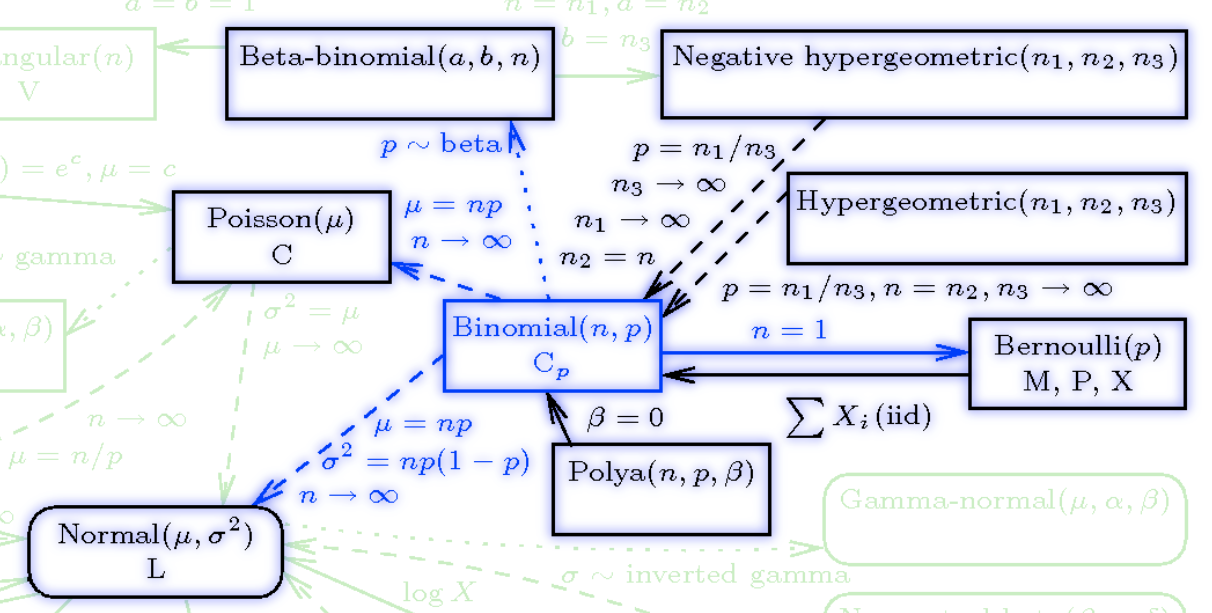
\includegraphics[width=53mm,height=\textheight,keepaspectratio]{images/dbinomial.png}

}

\caption{\label{fig-dbinomial}binomial distribution relations}

\end{marginfigure}%

The Binomial Distribution is related to:

\begin{itemize}
\tightlist
\item
  the \textbf{Geometric distribution},
\item
  The \textbf{Multinomial distribution} \index{distribution!multinomial}
  with two categories is the binomial.
\item
  the \textbf{Poisson distribution} \index{distribution!Poisson}
  distribution. If \(X \sim \mathrm{Binomial}(n, p)\) rv and
  \(Y \sim \mathrm{Poisson}(np)\) distribution then
  \(\mathbb{P}r(X = n) \approx \mathbb{P}r(Y = n)\) for large \(n\) and
  small \(np\).
\item
  the \textbf{Bernoulli distribution} If
  \(X \sim \mathrm{Binomial}(n, p)\) RV with \(n = 1\),
  \(X \sim Bernoulli(p)\) RV.
\item
  the \textbf{Normal distribution} If \(X \sim \mathrm{Binomial}(n, p)\)
  RV and \(Y \sim Normal(\mu=np,\sigma=n\mathbb{P}r(1-p))\) then for
  integers j and k,
  \(\mathbb{P}r(j \le X \le k) \approx \mathbb{P}r(j – {1 \over 2} \le Y \le k + {1 \over 2})\).
  The approximation is better when \(p ≈ 0.5\) and when n is large. For
  more information, see normal approximation to binomial
\item
  \textbf{Hypergeometric}: The difference between a binomial
  distribution and a hypergeometric distribution is the difference
  between sampling with replacement and sampling without replacement. As
  the population size increases relative to the sample size, the
  difference becomes negligible. So If \(X \sim Binomial(n, p)\) RV and
  \(Y \sim HyperGeometric(N,a,b)\) then
\end{itemize}

\[
\lim_{n\to \infty} X = Y 
\]

\begin{Shaded}
\begin{Highlighting}[]
\ImportTok{import}\NormalTok{ numpy }\ImportTok{as}\NormalTok{ np}
\ImportTok{from}\NormalTok{ scipy.stats }\ImportTok{import}\NormalTok{ binom}
\ImportTok{import}\NormalTok{ matplotlib.pyplot }\ImportTok{as}\NormalTok{ plt}

\NormalTok{fig, ax }\OperatorTok{=}\NormalTok{ plt.subplots(}\DecValTok{1}\NormalTok{, }\DecValTok{1}\NormalTok{)}
\NormalTok{n, p }\OperatorTok{=} \DecValTok{5}\NormalTok{, }\FloatTok{0.4}
\NormalTok{mean, var, skew, kurt }\OperatorTok{=}\NormalTok{ binom.stats(n, p, moments}\OperatorTok{=}\StringTok{\textquotesingle{}mvsk\textquotesingle{}}\NormalTok{)}
\BuiltInTok{print}\NormalTok{(}\SpecialStringTok{f\textquotesingle{}}\SpecialCharTok{\{}\NormalTok{mean}\OperatorTok{=}\SpecialCharTok{:1.2f\}}\SpecialStringTok{, }\SpecialCharTok{\{}\NormalTok{var}\OperatorTok{=}\SpecialCharTok{:1.2f\}}\SpecialStringTok{, }\SpecialCharTok{\{}\NormalTok{skew}\OperatorTok{=}\SpecialCharTok{:1.2f\}}\SpecialStringTok{, }\SpecialCharTok{\{}\NormalTok{kurt}\OperatorTok{=}\SpecialCharTok{:1.2f\}}\SpecialStringTok{\textquotesingle{}}\NormalTok{)}
\end{Highlighting}
\end{Shaded}

\begin{verbatim}
mean=2.00, var=1.20, skew=0.18, kurt=-0.37
\end{verbatim}

\begin{Shaded}
\begin{Highlighting}[]
\NormalTok{x }\OperatorTok{=}\NormalTok{ np.arange(binom.ppf(}\FloatTok{0.01}\NormalTok{, n, p), binom.ppf(}\FloatTok{0.99}\NormalTok{, n, p))}
\NormalTok{ax.plot(x, binom.pmf(x, n, p), }\StringTok{\textquotesingle{}bo\textquotesingle{}}\NormalTok{, ms}\OperatorTok{=}\DecValTok{8}\NormalTok{, label}\OperatorTok{=}\StringTok{\textquotesingle{}binom pmf\textquotesingle{}}\NormalTok{)}
\NormalTok{ax.vlines(x, }\DecValTok{0}\NormalTok{, binom.pmf(x, n, p), colors}\OperatorTok{=}\StringTok{\textquotesingle{}b\textquotesingle{}}\NormalTok{, lw}\OperatorTok{=}\DecValTok{5}\NormalTok{, alpha}\OperatorTok{=}\FloatTok{0.5}\NormalTok{)}
\NormalTok{rv }\OperatorTok{=}\NormalTok{ binom(n, p)}
\NormalTok{ax.vlines(x, }\DecValTok{0}\NormalTok{, rv.pmf(x), colors}\OperatorTok{=}\StringTok{\textquotesingle{}k\textquotesingle{}}\NormalTok{, linestyles}\OperatorTok{=}\StringTok{\textquotesingle{}{-}\textquotesingle{}}\NormalTok{, lw}\OperatorTok{=}\DecValTok{1}\NormalTok{,}
\NormalTok{        label}\OperatorTok{=}\StringTok{\textquotesingle{}frozen pmf\textquotesingle{}}\NormalTok{)}
\NormalTok{ax.legend(loc}\OperatorTok{=}\StringTok{\textquotesingle{}best\textquotesingle{}}\NormalTok{, frameon}\OperatorTok{=}\VariableTok{False}\NormalTok{)}
\NormalTok{plt.show()}
\end{Highlighting}
\end{Shaded}

\pandocbounded{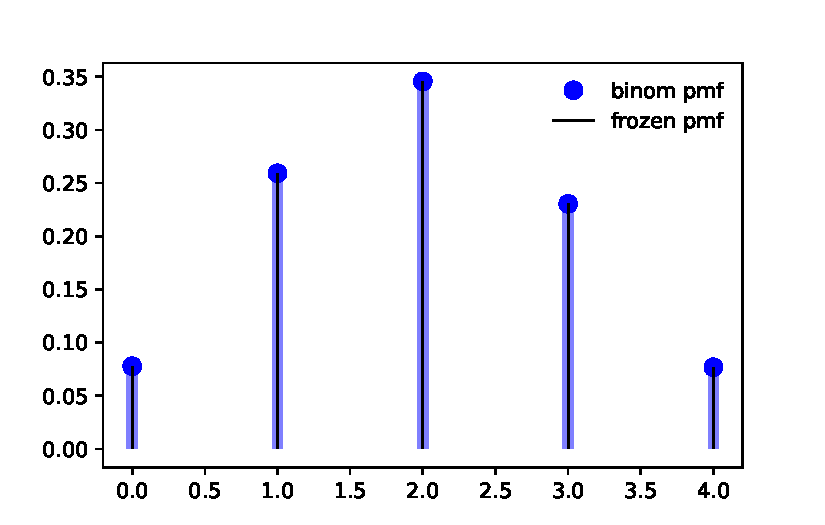
\includegraphics[keepaspectratio]{C1-L03_files/figure-pdf/binomial-distribution-3.pdf}}

\begin{Shaded}
\begin{Highlighting}[]
\CommentTok{\#\# generate random numbers}
\NormalTok{r }\OperatorTok{=}\NormalTok{ binom.rvs(n, p, size}\OperatorTok{=}\DecValTok{10}\NormalTok{)}
\NormalTok{r}
\end{Highlighting}
\end{Shaded}

\begin{verbatim}
array([1, 1, 3, 0, 1, 5, 3, 2, 3, 1])
\end{verbatim}

\subsection{The Discrete Uniform
Distribution}\label{the-discrete-uniform-distribution}

\begin{equation}\phantomsection\label{eq-l3-discrete-uniform-rv}{
X \sim U[0,1]
}\end{equation}

\begin{equation}\phantomsection\label{eq-l3-uniform-pmf}{
    f(x)=
    \begin{cases}
      1, & \text{if}\ x \in [0,1] \\
      0, & \text{otherwise}
    \end{cases}
    = \mathbb{I}_{\{0 \le x \le 1\}}(x)
}\end{equation}

\begin{Shaded}
\begin{Highlighting}[]
\ImportTok{import}\NormalTok{ numpy }\ImportTok{as}\NormalTok{ np}
\ImportTok{from}\NormalTok{ scipy.stats }\ImportTok{import}\NormalTok{ uniform}
\ImportTok{import}\NormalTok{ matplotlib.pyplot }\ImportTok{as}\NormalTok{ plt}
\NormalTok{fig, ax }\OperatorTok{=}\NormalTok{ plt.subplots(}\DecValTok{1}\NormalTok{, }\DecValTok{1}\NormalTok{)}

\NormalTok{n, p }\OperatorTok{=} \DecValTok{5}\NormalTok{, }\FloatTok{0.4}
\NormalTok{mean, var, skew, kurt }\OperatorTok{=}\NormalTok{ uniform.stats(moments}\OperatorTok{=}\StringTok{\textquotesingle{}mvsk\textquotesingle{}}\NormalTok{)}
\BuiltInTok{print}\NormalTok{(}\SpecialStringTok{f\textquotesingle{}}\SpecialCharTok{\{}\NormalTok{mean}\OperatorTok{=}\SpecialCharTok{:1.2f\}}\SpecialStringTok{, }\SpecialCharTok{\{}\NormalTok{var}\OperatorTok{=}\SpecialCharTok{:1.2f\}}\SpecialStringTok{, }\SpecialCharTok{\{}\NormalTok{skew}\OperatorTok{=}\SpecialCharTok{:1.2f\}}\SpecialStringTok{, }\SpecialCharTok{\{}\NormalTok{kurt}\OperatorTok{=}\SpecialCharTok{:1.2f\}}\SpecialStringTok{\textquotesingle{}}\NormalTok{)}
\end{Highlighting}
\end{Shaded}

\begin{verbatim}
mean=0.50, var=0.08, skew=0.00, kurt=-1.20
\end{verbatim}

\begin{Shaded}
\begin{Highlighting}[]
\CommentTok{\# we use ppf to get the domain from a range of (0.01,0.99)}
\NormalTok{x }\OperatorTok{=}\NormalTok{ np.linspace(uniform.ppf(}\FloatTok{0.01}\NormalTok{), uniform.ppf(}\FloatTok{0.99}\NormalTok{), }\DecValTok{100}\NormalTok{)}
\NormalTok{ax.plot(x, uniform.pdf(x), }\StringTok{\textquotesingle{}r{-}\textquotesingle{}}\NormalTok{, lw}\OperatorTok{=}\DecValTok{5}\NormalTok{, alpha}\OperatorTok{=}\FloatTok{0.6}\NormalTok{, label}\OperatorTok{=}\StringTok{\textquotesingle{}uniform pdf\textquotesingle{}}\NormalTok{)}
\NormalTok{rv }\OperatorTok{=}\NormalTok{ uniform()}
\NormalTok{ax.plot(x, rv.pdf(x), }\StringTok{\textquotesingle{}k{-}\textquotesingle{}}\NormalTok{, lw}\OperatorTok{=}\DecValTok{2}\NormalTok{, label}\OperatorTok{=}\StringTok{\textquotesingle{}frozen pdf\textquotesingle{}}\NormalTok{)}

\CommentTok{\#\# generate random numbers}
\NormalTok{r }\OperatorTok{=}\NormalTok{ uniform.rvs(size}\OperatorTok{=}\DecValTok{1000}\NormalTok{)}

\CommentTok{\# And compare the histogram:}
\NormalTok{ax.hist(r, density}\OperatorTok{=}\VariableTok{True}\NormalTok{, bins}\OperatorTok{=}\StringTok{\textquotesingle{}auto\textquotesingle{}}\NormalTok{, histtype}\OperatorTok{=}\StringTok{\textquotesingle{}stepfilled\textquotesingle{}}\NormalTok{, alpha}\OperatorTok{=}\FloatTok{0.2}\NormalTok{)}
\end{Highlighting}
\end{Shaded}

\begin{verbatim}
(array([1.12277226, 0.82556784, 1.02370412, 0.96866627, 1.16680255,
       1.11176469, 1.14478741, 0.99068141, 0.94665112, 0.83657541,
       0.86959813]), array([9.49782253e-06, 9.08560598e-02, 1.81702622e-01, 2.72549184e-01,
       3.63395746e-01, 4.54242308e-01, 5.45088869e-01, 6.35935431e-01,
       7.26781993e-01, 8.17628555e-01, 9.08475117e-01, 9.99321679e-01]), [<matplotlib.patches.Polygon object at 0x7f87b2a020b0>])
\end{verbatim}

\begin{Shaded}
\begin{Highlighting}[]
\NormalTok{ax.set\_xlim([x[}\DecValTok{0}\NormalTok{], x[}\OperatorTok{{-}}\DecValTok{1}\NormalTok{]])}
\end{Highlighting}
\end{Shaded}

\begin{verbatim}
(0.01, 0.99)
\end{verbatim}

\begin{Shaded}
\begin{Highlighting}[]
\NormalTok{ax.legend(loc}\OperatorTok{=}\StringTok{\textquotesingle{}best\textquotesingle{}}\NormalTok{, frameon}\OperatorTok{=}\VariableTok{False}\NormalTok{)}
\NormalTok{plt.show()}
\end{Highlighting}
\end{Shaded}

\pandocbounded{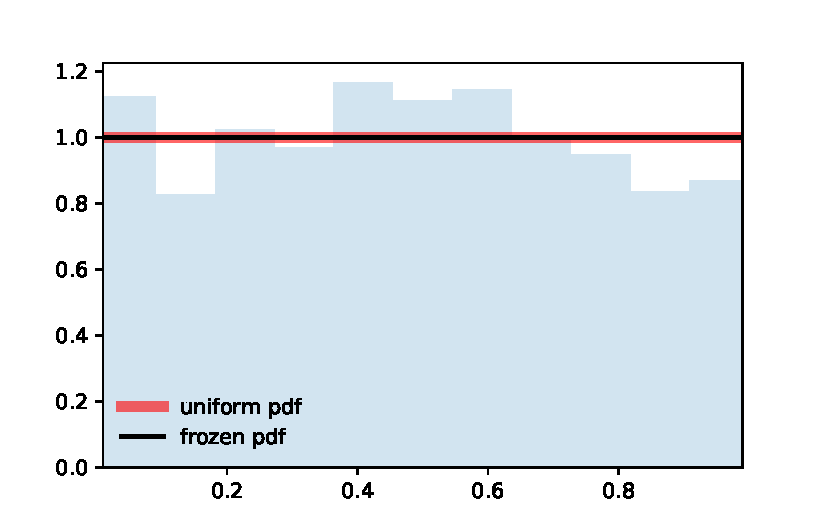
\includegraphics[keepaspectratio]{C1-L03_files/figure-pdf/uniform-distribution-5.pdf}}

\subsection{The Continuous Uniform
Distribution}\label{the-continuous-uniform-distribution}

\begin{equation}\phantomsection\label{eq-l3-uniform-rv}{
X \sim \mathrm{Uniform}[\theta_1,\theta_2] 
}\end{equation}

\begin{equation}\phantomsection\label{eq-l3-uniform-pdf}{
f(x)= \frac{1}{\theta_2-\theta_1} \mathbb{I}_{\{\theta_1 \le x \le \theta_2\}}(x) 
}\end{equation}

\section{The Normal, Z, t
Distributions}\label{sec-the-normal-z-t-distributions}

\index{distribution!normal} The \emph{normal}, AKA \emph{Gaussian
distribution} is one of the most important distributions in statistics.

It arises as the limiting distribution of sums (and averages) of random
variables. This is due to the Section~\ref{sec-cl-theorem}. Because of
this property, the normal distribution is often used to model the
``errors,'' or unexplained variations of individual observations in
regression models.

\subsection{The Standard Normal
distribution}\label{sec-the-standard-normal-distribution}

\index{distribution!standard normal} The standard normal distribution is
given by

\begin{equation}\phantomsection\label{eq-l3-z-rv}{
\mathcal{Z} \sim \mathcal{N}[1,0]
}\end{equation}

\begin{equation}\phantomsection\label{eq-l3-z-pdf}{
f(z) = \frac{1}{\sqrt{2 \pi}} e^{-\frac{z^2}{2}}
}\end{equation}

\begin{equation}\phantomsection\label{eq-l3-z-expectation}{
\mathbb{E}[\mathcal{Z}] = 0
}\end{equation}

\begin{equation}\phantomsection\label{eq-l3-z-variance}{
\mathbb{V}ar[\mathcal{Z}]= 1
}\end{equation}

\subsection{The Normal distribution}\label{the-normal-distribution}

\index{distribution!normal} Now consider \(X = \sigma \mathcal{Z}+\mu\)
where \(\sigma > 0\) and \(\mu\) is any real constant. Then
\(\mathbb{E}(X) = \mathbb{E}(\sigma \mathcal{Z}+\mu) = \sigma \mathbb{E}(\mathcal{Z}) + \mu = \sigma \times 0 + \mu = \mu\)
and
\(Var(X) = Var(\sigma^2 + \mu) = \sigma^2 Var(\mathcal{Z}) + 0 = \sigma^2 \cdot 1 = \sigma^2\)

Then, X follows a normal distribution with mean \(\mu\) and variance
\(\sigma^2\) (standard deviation \(\sigma\)) denoted as

\begin{equation}\phantomsection\label{eq-l3-normal-rv}{
X \sim \mathcal{N}[\mu,\sigma^2]
}\end{equation}

\begin{equation}\phantomsection\label{eq-l3-normal-pdf}{
f(x\mid \mu,\sigma^2) = \frac{1}{\sqrt{2 \pi \sigma^2}}  e^{-\frac{1}{\sqrt{2 \pi \sigma^2}}(x-\mu)^2}
}\end{equation}

\begin{equation}\phantomsection\label{eq-l3-normal-expectation}{
\mathbb{E}[x]= \mu 
}\end{equation}

\begin{equation}\phantomsection\label{eq-l3-normal-variance}{
\mathbb{V}ar[x]= \sigma^2
}\end{equation}

\begin{itemize}
\tightlist
\item
  The normal distribution is symmetric about the mean \(\mu\) and is
  often described as a \texttt{bell-shaped} curve.
\item
  Although X can take on any real value (positive or negative), more
  than 99\% of the probability mass is concentrated within three
  standard deviations of the mean.
\end{itemize}

The normal distribution has several desirable properties.

One is that if \(X_1 \sim \mathcal{N}(\mu_1, \sigma^2_1)\) and
\(X_2 \sim \mathcal{N}(\mu_2, \sigma^2_2)\) are independent, then
\(X_1+X_2 \sim \mathcal{N}(\mu_1+\mu_2, \sigma^2_1+\sigma^2_2)\).

Consequently, if we take the average of n Independent and Identically
Distributed (IID) normal random variables we have

\begin{equation}\phantomsection\label{eq-l3-normal-sum}{
\bar X = \frac{1}{n}\sum_{i=1}^n X_i \sim \mathcal{N}(\mu, \frac{\sigma^2}{n})
}\end{equation}

\begin{Shaded}
\begin{Highlighting}[]
\ImportTok{import}\NormalTok{ numpy }\ImportTok{as}\NormalTok{ np}
\ImportTok{from}\NormalTok{ scipy.stats }\ImportTok{import}\NormalTok{ norm}
\ImportTok{import}\NormalTok{ matplotlib.pyplot }\ImportTok{as}\NormalTok{ plt}
\NormalTok{fig, ax }\OperatorTok{=}\NormalTok{ plt.subplots(}\DecValTok{1}\NormalTok{, }\DecValTok{1}\NormalTok{)}

\NormalTok{n, p }\OperatorTok{=} \DecValTok{5}\NormalTok{, }\FloatTok{0.4}
\NormalTok{mean, var, skew, kurt }\OperatorTok{=}\NormalTok{ norm.stats(moments}\OperatorTok{=}\StringTok{\textquotesingle{}mvsk\textquotesingle{}}\NormalTok{)}
\BuiltInTok{print}\NormalTok{(}\SpecialStringTok{f\textquotesingle{}}\SpecialCharTok{\{}\NormalTok{mean}\OperatorTok{=}\SpecialCharTok{:1.2f\}}\SpecialStringTok{, }\SpecialCharTok{\{}\NormalTok{var}\OperatorTok{=}\SpecialCharTok{:1.2f\}}\SpecialStringTok{, }\SpecialCharTok{\{}\NormalTok{skew}\OperatorTok{=}\SpecialCharTok{:1.2f\}}\SpecialStringTok{, }\SpecialCharTok{\{}\NormalTok{kurt}\OperatorTok{=}\SpecialCharTok{:1.2f\}}\SpecialStringTok{\textquotesingle{}}\NormalTok{)}
\end{Highlighting}
\end{Shaded}

\begin{verbatim}
mean=0.00, var=1.00, skew=0.00, kurt=0.00
\end{verbatim}

\begin{Shaded}
\begin{Highlighting}[]
\NormalTok{x }\OperatorTok{=}\NormalTok{ np.linspace(norm.ppf(}\FloatTok{0.01}\NormalTok{),}
\NormalTok{                norm.ppf(}\FloatTok{0.99}\NormalTok{), }\DecValTok{100}\NormalTok{)}
\NormalTok{ax.plot(x, norm.pdf(x),}
       \StringTok{\textquotesingle{}r{-}\textquotesingle{}}\NormalTok{, lw}\OperatorTok{=}\DecValTok{5}\NormalTok{, alpha}\OperatorTok{=}\FloatTok{0.6}\NormalTok{, label}\OperatorTok{=}\StringTok{\textquotesingle{}norm pdf\textquotesingle{}}\NormalTok{)}

\NormalTok{rv }\OperatorTok{=}\NormalTok{ norm()}
\NormalTok{ax.plot(x, rv.pdf(x), }\StringTok{\textquotesingle{}k{-}\textquotesingle{}}\NormalTok{, lw}\OperatorTok{=}\DecValTok{2}\NormalTok{, label}\OperatorTok{=}\StringTok{\textquotesingle{}frozen pdf\textquotesingle{}}\NormalTok{)}
\NormalTok{r }\OperatorTok{=}\NormalTok{ norm.rvs(size}\OperatorTok{=}\DecValTok{1000}\NormalTok{)}

\NormalTok{ax.hist(r, density}\OperatorTok{=}\VariableTok{True}\NormalTok{, bins}\OperatorTok{=}\StringTok{\textquotesingle{}auto\textquotesingle{}}\NormalTok{, histtype}\OperatorTok{=}\StringTok{\textquotesingle{}stepfilled\textquotesingle{}}\NormalTok{, alpha}\OperatorTok{=}\FloatTok{0.2}\NormalTok{)}
\end{Highlighting}
\end{Shaded}

\begin{verbatim}
(array([0.01107987, 0.00738658, 0.03323961, 0.0369329 , 0.06278593,
       0.10341212, 0.11449199, 0.26961017, 0.27330346, 0.37302229,
       0.369329  , 0.39887532, 0.35455584, 0.33608939, 0.36563571,
       0.20313095, 0.12926515, 0.08125238, 0.06647922, 0.06278593,
       0.02954632, 0.        , 0.        , 0.00738658, 0.00369329]), array([-3.07755318, -2.80679188, -2.53603058, -2.26526928, -1.99450798,
       -1.72374668, -1.45298539, -1.18222409, -0.91146279, -0.64070149,
       -0.36994019, -0.09917889,  0.17158241,  0.44234371,  0.713105  ,
        0.9838663 ,  1.2546276 ,  1.5253889 ,  1.7961502 ,  2.0669115 ,
        2.3376728 ,  2.6084341 ,  2.87919539,  3.14995669,  3.42071799,
        3.69147929]), [<matplotlib.patches.Polygon object at 0x7f87b2a591b0>])
\end{verbatim}

\begin{Shaded}
\begin{Highlighting}[]
\NormalTok{ax.set\_xlim([x[}\DecValTok{0}\NormalTok{], x[}\OperatorTok{{-}}\DecValTok{1}\NormalTok{]])}
\end{Highlighting}
\end{Shaded}

\begin{verbatim}
(-2.3263478740408408, 2.3263478740408408)
\end{verbatim}

\begin{Shaded}
\begin{Highlighting}[]
\NormalTok{ax.legend(loc}\OperatorTok{=}\StringTok{\textquotesingle{}best\textquotesingle{}}\NormalTok{, frameon}\OperatorTok{=}\VariableTok{False}\NormalTok{)}
\NormalTok{plt.show()}
\end{Highlighting}
\end{Shaded}

\pandocbounded{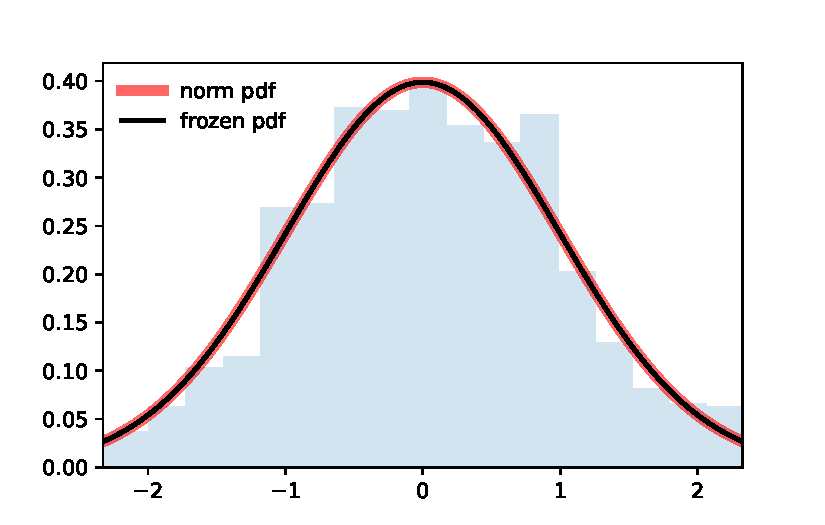
\includegraphics[keepaspectratio]{C1-L03_files/figure-pdf/normal-distribution-7.pdf}}

\subsection{The t-Distribution}\label{the-t-distribution}

\index{distribution,t} If we have normal data, we can use
(Equation~\ref{eq-normal-sum}) to help us estimate the mean \(\mu\).
Reversing the transformation from the previous section, we get

\begin{equation}\phantomsection\label{eq-l3-t-transform}{
\frac {\hat X - \mu}{\sigma / \sqrt(n)} \sim N(0, 1)
}\end{equation}

However, we may not know the value of \(\sigma\). If we estimate it from
data, we can replace it with
\(S = \sqrt{\sum_i \frac{(X_i-\hat X)^2}{n-1}}\), the sample standard
deviation. This causes the expression (Equation~\ref{eq-t-transform}) to
no longer be distributed as a Standard Normal; but as a standard
\emph{t-distribution} with \(ν = n − 1\) \texttt{degrees\ of\ freedom}

\begin{equation}\phantomsection\label{eq-l3-t-rv}{
X \sim t[\nu]
}\end{equation}

\begin{equation}\phantomsection\label{eq-l3-t-pdf-gamma}{
f(t\mid\nu) = \frac{\Gamma(\frac{\nu+1}{2})}{\Gamma(\frac{\nu}{2})\sqrt{\nu\pi}}\left (1 + \frac{t^2}{\nu}\right)^{-(\frac{\nu+1}{2})}\mathbb{I}_{t\in\mathbb{R}} \qquad \text{(PDF)}
}\end{equation}

\[
\text{where }\Gamma(w)=\int_{0}^{\infty}t^{w-1}e^{-t}\mathrm{d}t \text{ is the gamma function}
\]

\begin{equation}\phantomsection\label{eq-l3-t-pdf-beta}{
f(t\mid\nu)={\frac {1}{{\sqrt {\nu }}\,\mathrm {B} ({\frac {1}{2}},{\frac {\nu }{2}})}}\left(1+{\frac {t^{2}}{\nu }}\right)^{-(\nu +1)/2}\mathbb{I}_{t\in\mathbb{R}} \qquad \text{(PDF)}
}\end{equation}

\[
\text{where } B(u,v)=\int_{0}^{1}t^{u-1}(1-t)^{v-1}\mathrm{d}t \text{ is the beta function}
\]

\begin{equation}\phantomsection\label{eq-l3-t-expectation-xyz}{
\mathbb{E}[Y] = 0 \qquad \text{ if } \nu > 1
}\end{equation}

\begin{equation}\phantomsection\label{eq-l3-t-variance}{
\mathbb{V}ar[Y] = \frac{\nu}{\nu - 2} \qquad \text{ if } \nu > 2
}\end{equation}

The t distribution is symmetric and resembles the Normal Distribution
but with thicker tails. As the degrees of freedom increase, the t
distribution looks more and more like the standard normal distribution.

\section{The Exponential
Distribution}\label{the-exponential-distribution}

\index{Exponential distribution} The \textbf{Exponential distribution}
models the waiting time between events for events with a rate
\(\lambda\). Those events, typically, come from a \textbf{Poisson}
process.

The \textbf{Exponential distribution} is often used to model the
\texttt{waiting\ time\ between\ random\ events}. Indeed, if the waiting
times between successive events are independent then they form an
\(\exp(r(\lambda)\) distribution. Then for any fixed time window of
length t, the number of events occurring in that window will follow a
\texttt{Poisson\ distribution} with mean \(t\lambda\).

\begin{equation}\phantomsection\label{eq-l3-exponential-rv}{
X \sim Exp[\lambda]
}\end{equation}

\begin{equation}\phantomsection\label{eq-l3-exponential-pdf}{
f(x \mid \lambda) = \frac{1}{\lambda} e^{- \frac{x}{\lambda}}(x)\mathbb{I}_{\lambda\in\mathbb{R}^+ } \mathbb{I}_{x\in\mathbb{R}^+_0 } \quad \text{(PDF)}
}\end{equation}

\begin{equation}\phantomsection\label{eq-l3-exponential-expectation}{
\mathbb{E}(x)= \lambda
}\end{equation}

\begin{equation}\phantomsection\label{eq-l3-exponential-variance}{
\mathbb{V}ar[X]= \lambda^2
}\end{equation}

\begin{Shaded}
\begin{Highlighting}[]
\ImportTok{import}\NormalTok{ numpy }\ImportTok{as}\NormalTok{ np}
\ImportTok{from}\NormalTok{ scipy.stats }\ImportTok{import}\NormalTok{ expon}
\ImportTok{import}\NormalTok{ matplotlib.pyplot }\ImportTok{as}\NormalTok{ plt}
\NormalTok{fig, ax }\OperatorTok{=}\NormalTok{ plt.subplots(}\DecValTok{1}\NormalTok{, }\DecValTok{1}\NormalTok{)}

\NormalTok{n, p }\OperatorTok{=} \DecValTok{5}\NormalTok{, }\FloatTok{0.4}
\NormalTok{mean, var, skew, kurt }\OperatorTok{=}\NormalTok{ expon.stats(moments}\OperatorTok{=}\StringTok{\textquotesingle{}mvsk\textquotesingle{}}\NormalTok{)}
\BuiltInTok{print}\NormalTok{(}\SpecialStringTok{f\textquotesingle{}}\SpecialCharTok{\{}\NormalTok{mean}\OperatorTok{=}\SpecialCharTok{:1.2f\}}\SpecialStringTok{, }\SpecialCharTok{\{}\NormalTok{var}\OperatorTok{=}\SpecialCharTok{:1.2f\}}\SpecialStringTok{, }\SpecialCharTok{\{}\NormalTok{skew}\OperatorTok{=}\SpecialCharTok{:1.2f\}}\SpecialStringTok{, }\SpecialCharTok{\{}\NormalTok{kurt}\OperatorTok{=}\SpecialCharTok{:1.2f\}}\SpecialStringTok{\textquotesingle{}}\NormalTok{)}
\end{Highlighting}
\end{Shaded}

\begin{verbatim}
mean=1.00, var=1.00, skew=2.00, kurt=6.00
\end{verbatim}

\begin{Shaded}
\begin{Highlighting}[]
\NormalTok{x }\OperatorTok{=}\NormalTok{ np.linspace(expon.ppf(}\FloatTok{0.01}\NormalTok{), expon.ppf(}\FloatTok{0.99}\NormalTok{), }\DecValTok{100}\NormalTok{)}
\NormalTok{ax.plot(x, expon.pdf(x), }\StringTok{\textquotesingle{}r{-}\textquotesingle{}}\NormalTok{, lw}\OperatorTok{=}\DecValTok{5}\NormalTok{, alpha}\OperatorTok{=}\FloatTok{0.6}\NormalTok{, label}\OperatorTok{=}\StringTok{\textquotesingle{}expon pdf\textquotesingle{}}\NormalTok{)}

\NormalTok{rv }\OperatorTok{=}\NormalTok{ expon()}
\NormalTok{ax.plot(x, rv.pdf(x), }\StringTok{\textquotesingle{}k{-}\textquotesingle{}}\NormalTok{, lw}\OperatorTok{=}\DecValTok{2}\NormalTok{, label}\OperatorTok{=}\StringTok{\textquotesingle{}frozen pdf\textquotesingle{}}\NormalTok{)}

\NormalTok{r }\OperatorTok{=}\NormalTok{ expon.rvs(size}\OperatorTok{=}\DecValTok{1000}\NormalTok{)}

\NormalTok{ax.hist(r, density}\OperatorTok{=}\VariableTok{True}\NormalTok{, bins}\OperatorTok{=}\StringTok{\textquotesingle{}auto\textquotesingle{}}\NormalTok{, histtype}\OperatorTok{=}\StringTok{\textquotesingle{}stepfilled\textquotesingle{}}\NormalTok{, alpha}\OperatorTok{=}\FloatTok{0.2}\NormalTok{)}
\end{Highlighting}
\end{Shaded}

\begin{verbatim}
(array([0.90823976, 0.70077383, 0.53019072, 0.47025612, 0.35499727,
       0.34577656, 0.29967302, 0.17519346, 0.17980381, 0.10142779,
       0.13370027, 0.09220708, 0.06454496, 0.0599346 , 0.04149319,
       0.00922071, 0.02766212, 0.04610354, 0.01844142, 0.00922071,
       0.00461035, 0.00461035, 0.00461035, 0.00461035, 0.        ,
       0.00461035, 0.00461035, 0.00461035, 0.        , 0.        ,
       0.        , 0.00461035, 0.00461035]), array([5.21795661e-03, 2.22121035e-01, 4.39024113e-01, 6.55927191e-01,
       8.72830269e-01, 1.08973335e+00, 1.30663643e+00, 1.52353950e+00,
       1.74044258e+00, 1.95734566e+00, 2.17424874e+00, 2.39115182e+00,
       2.60805489e+00, 2.82495797e+00, 3.04186105e+00, 3.25876413e+00,
       3.47566721e+00, 3.69257029e+00, 3.90947336e+00, 4.12637644e+00,
       4.34327952e+00, 4.56018260e+00, 4.77708568e+00, 4.99398875e+00,
       5.21089183e+00, 5.42779491e+00, 5.64469799e+00, 5.86160107e+00,
       6.07850415e+00, 6.29540722e+00, 6.51231030e+00, 6.72921338e+00,
       6.94611646e+00, 7.16301954e+00]), [<matplotlib.patches.Polygon object at 0x7f87b28fc130>])
\end{verbatim}

\begin{Shaded}
\begin{Highlighting}[]
\NormalTok{ax.set\_xlim([x[}\DecValTok{0}\NormalTok{], x[}\OperatorTok{{-}}\DecValTok{1}\NormalTok{]])}
\end{Highlighting}
\end{Shaded}

\begin{verbatim}
(0.010050335853501442, 4.605170185988091)
\end{verbatim}

\begin{Shaded}
\begin{Highlighting}[]
\NormalTok{ax.legend(loc}\OperatorTok{=}\StringTok{\textquotesingle{}best\textquotesingle{}}\NormalTok{, frameon}\OperatorTok{=}\VariableTok{False}\NormalTok{)}
\NormalTok{plt.show()}
\end{Highlighting}
\end{Shaded}

\pandocbounded{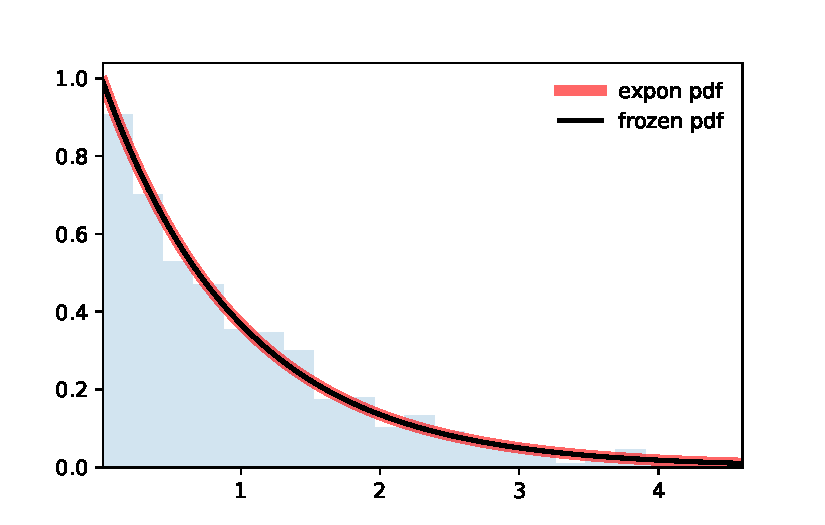
\includegraphics[keepaspectratio]{C1-L03_files/figure-pdf/exponential-distribution-9.pdf}}

\chapter{Additional Discrete
Distributions}\label{additional-discrete-distributions}

\section{The Geometric
Distribution}\label{sec-the-geometric-distribution}

\index{distribution!geometric} The \textbf{Geometric distribution}
arises when we want to know ``What is the number of Bernoulli trials
required to get the first success?'', i.e., the number of Bernoulli
events until a success is observed, such as the probability of getting
the first head when flipping a coin. It takes values on the positive
integers starting with one (since at least one trial is needed to
observe a success).

\begin{equation}\phantomsection\label{eq-l3-geom-rv}{
X \sim \mathrm{Geo}(p)
}\end{equation}

\begin{equation}\phantomsection\label{eq-l3-geom-pmf}{
\mathbb{P}r(X = x\mid p) = \mathbb{P}r(1-p)^{x-1} \qquad \forall x \in N;\quad 0\le p \le 1 
}\end{equation}

\begin{equation}\phantomsection\label{eq-l3-geom-expectation}{
\mathbb{E}[X] = \frac{1}{p}
}\end{equation}

\begin{equation}\phantomsection\label{eq-l3-geom-variance}{
\mathbb{V}ar[X]=\frac{1-p}{p^2}
}\end{equation}

\begin{equation}\phantomsection\label{eq-l3-geom-mgf}{
\mathbb{M}_X[t] = \frac{pe^t}{1-(1-p)e^t} \qquad t < -log(1-p)
}\end{equation}

\section{The Multinomial
Distribution}\label{sec-the-multinomial-distribution}

\index{distribution!multinomial} \index{distribution!Bernoulli} Another
generalization of the Bernoulli distribution and the Binomial
distribution is the \textbf{Multinomial distribution}, which sums the
successes of Bernoulli trials when there are n different possible
outcomes. Suppose we have n trials and there are k different possible
outcomes that occur with probabilities \(p_1, \ldots, p_k\). For
example, we are rolling a six-sided die that might be loaded so that the
sides are not equally likely, then n is the total number of rolls,
\(k = 6\), \(p_1\) is the probability of rolling a one, and we denote by
\(x_1, \ldots, x_6\) a possible outcome for the number of times we
observe rolls of each of one through six, where

\[
X \sim \mathrm{Multinomial}(p_1,...p_k)
\]

\[
P (X = x \mid p_1,\ldots,p_k) = \frac{n!}{x_1! \cdot \cdot \cdot x_k! } \prod_i p_i^{x_i}
\]

\section{The Poisson Distribution}\label{sec-the-poisson-distribution}

The \textbf{Poisson distribution} \index{distribution!Poisson} arises
when modeling \textbf{count} data. The parameter \(\lambda > 0\) is the
\texttt{rate} at which we expect to observe the thing we are counting.
We write this as \(X \sim \mathrm{Poisson}(\lambda)\)

\begin{equation}\phantomsection\label{eq-l3-poisson-PMF}{
\mathbb{P}r(X = x \mid \lambda) = \frac{\lambda^x e^{−\lambda}}{x!} \qquad \forall x \in \mathbb{N}_0 \qquad \text{PDF}
}\end{equation}

\begin{equation}\phantomsection\label{eq-l3-poisson-expectation}{
\mathbb{E}[X] = \lambda \qquad \text{Expectation}
}\end{equation}

\begin{equation}\phantomsection\label{eq-l3-poisson-variance}{
\mathbb{V}ar[X] = \lambda \qquad \text{Variance}
}\end{equation}

\begin{equation}\phantomsection\label{eq-l3-poisson-mgf}{
\mathbb{M}_X(t) = \exp[\lambda(e^t-1)] \qquad \text{Moment Generating fn.}
}\end{equation}

\begin{equation}\phantomsection\label{eq-l3-poisson-fisher-information}{
\mathcal{I}_X(t) = \frac{1}{\lambda}
}\end{equation}

\subsection{Relations}\label{relations}

\begin{marginfigure}

\centering{

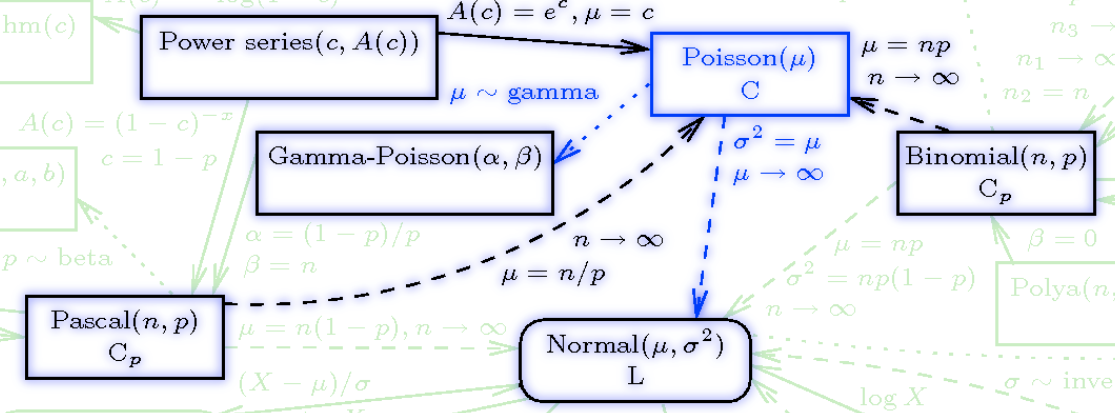
\includegraphics[width=53mm,height=\textheight,keepaspectratio]{images/dpoisson.png}

}

\caption{\label{fig-dPoisson}Relations of the Poisson distribution}

\end{marginfigure}%

\index{process!Poisson} A \emph{Poisson process} is a process wherein
events occur on average at rate \(\mathbb{E}\), events occur one at a
time, and events occur independently of each other.

\begin{marginfigure}

\centering{

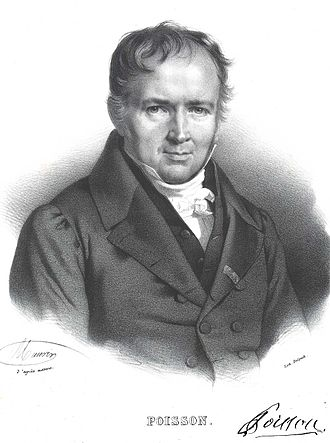
\includegraphics[width=53mm,height=\textheight,keepaspectratio]{images/bio-SimeonDenisPoisson.jpg}

}

\caption{\label{fig-bio-Poisson}Siméon Denis Poisson}

\end{marginfigure}%

\begin{tcolorbox}[enhanced jigsaw, bottomrule=.15mm, colbacktitle=quarto-callout-tip-color!10!white, leftrule=.75mm, bottomtitle=1mm, titlerule=0mm, title=\textcolor{quarto-callout-tip-color}{\faLightbulb}\hspace{0.5em}{Biographical Note on The Siméon Denis Poisson}, rightrule=.15mm, toprule=.15mm, colback=white, left=2mm, toptitle=1mm, arc=.35mm, opacitybacktitle=0.6, coltitle=black, breakable, opacityback=0, colframe=quarto-callout-tip-color-frame]

The Poisson distribution is due to Baron Siméon Denis Poisson
(1781-1840) see (Poisson 2019, 205--7) was a French mathematician and
physicist who worked on statistics, complex analysis, partial
differential equations, the calculus of variations, analytical
mechanics, electricity and magnetism, thermodynamics, elasticity, and
fluid mechanics.

for a fuller
\href{https://mathshistory.st-andrews.ac.uk/Biographies/Poisson/}{biography
see}

\end{tcolorbox}

\section{Hypergeometric Distribution}\label{hypergeometric-distribution}

\index{distribution!hypergeometric}

Consider an urn with \(a\) white balls and \(b\) black balls. Draw \(N\)
balls from this urn without replacement. The number white balls drawn,
\(n\) is Hypergeometrically distributed.

\[
X \sim \mathrm{Hypergeometric}(n \mid N,a,b)
\]

\begin{equation}\phantomsection\label{eq-l3-Hypergeometric-pdf}{
\mathrm{Hypergeometric}(n\mid N,a,b) = \frac{\normalsize{\binom{a}{n} \binom{b}{N - n}}} {\normalsize{\binom{a + b}{N}}} \quad \text{(PDF)}
}\end{equation}

\begin{equation}\phantomsection\label{eq-l3-Hypergeometric-expectation}{
\mathbb{E}[X]=N\frac{a}{a+b} \qquad \text{(expectation)}
}\end{equation}

\begin{equation}\phantomsection\label{eq-l3-Hypergeometric-variance}{
\mathbb{V}ar[X]=N\,\frac{ab}{(a + b)^2}\,\frac{a+b-N}{a+b-1} \qquad \text{(variance)}
}\end{equation}

\chapter{Random Variables - M1L3HW1}\label{random-variables---m1l3hw1}

Bayesian Statistics: From Concept to Data Analysis

\hfill\break

\begin{tcolorbox}[enhanced jigsaw, bottomrule=.15mm, colbacktitle=quarto-callout-caution-color!10!white, leftrule=.75mm, bottomtitle=1mm, titlerule=0mm, title=\textcolor{quarto-callout-caution-color}{\faFire}\hspace{0.5em}{Caution}, rightrule=.15mm, toprule=.15mm, colback=white, left=2mm, toptitle=1mm, arc=.35mm, opacitybacktitle=0.6, coltitle=black, breakable, opacityback=0, colframe=quarto-callout-caution-color-frame]

Section omitted to comply with the Honor Code

\end{tcolorbox}

\chapter{Homework on Distributions -
M1L3HW2}\label{homework-on-distributions---m1l3hw2}

Bayesian Statistics: From Concept to Data Analysis

\hfill\break

\begin{tcolorbox}[enhanced jigsaw, bottomrule=.15mm, colbacktitle=quarto-callout-caution-color!10!white, leftrule=.75mm, bottomtitle=1mm, titlerule=0mm, title=\textcolor{quarto-callout-caution-color}{\faFire}\hspace{0.5em}{Caution}, rightrule=.15mm, toprule=.15mm, colback=white, left=2mm, toptitle=1mm, arc=.35mm, opacitybacktitle=0.6, coltitle=black, breakable, opacityback=0, colframe=quarto-callout-caution-color-frame]

Section omitted to comply with the Honor Code

\end{tcolorbox}

\chapter{Frequentist Inference -
M2L4}\label{frequentist-inference---m2l4}

Bayesian Statistics: From Concept to Data Analysis

\hfill\break

\index{Maximum Likelihood Estimation} Before delving into Bayesian
inference in the next module, in this module we will review inference in
the frequentist approach. Much of the material was developed by R. A.
Fischer in the last century. Some of the central ideas and tools of this
approach include:

\begin{itemize}
\tightlist
\item
  Maximum Likelihood estimates MLE, which are point estimates of
  statistics.
\item
  Confidence intervals CIs which formalize uncertainty in this paradigm.
\item
  Likelihood functions and Log-likelihood functions which are the basis
  of MLE estimates.
\item
  Quantile Functions
\item
  Hypothesis testing
\item
  Reference Population
\end{itemize}

One point of interest is how much of this work is based on the law of
large numbers, central limit theorem and the empirical rule, three
related key results in probability theory.

However the second point to stress is that the \textbf{frequentist
paradigm} is fraught with practical as well as philosophical challenges
which are handled better to some extent within the Bayesian paradigm.

In particular, the frequentist paradigm does not allow us to make
probability statements about parameters, which is a key feature of the
Bayesian approach.

\section{Confidence Intervals}\label{sec-confidence-intervals}

\begin{marginfigure}

\centering{

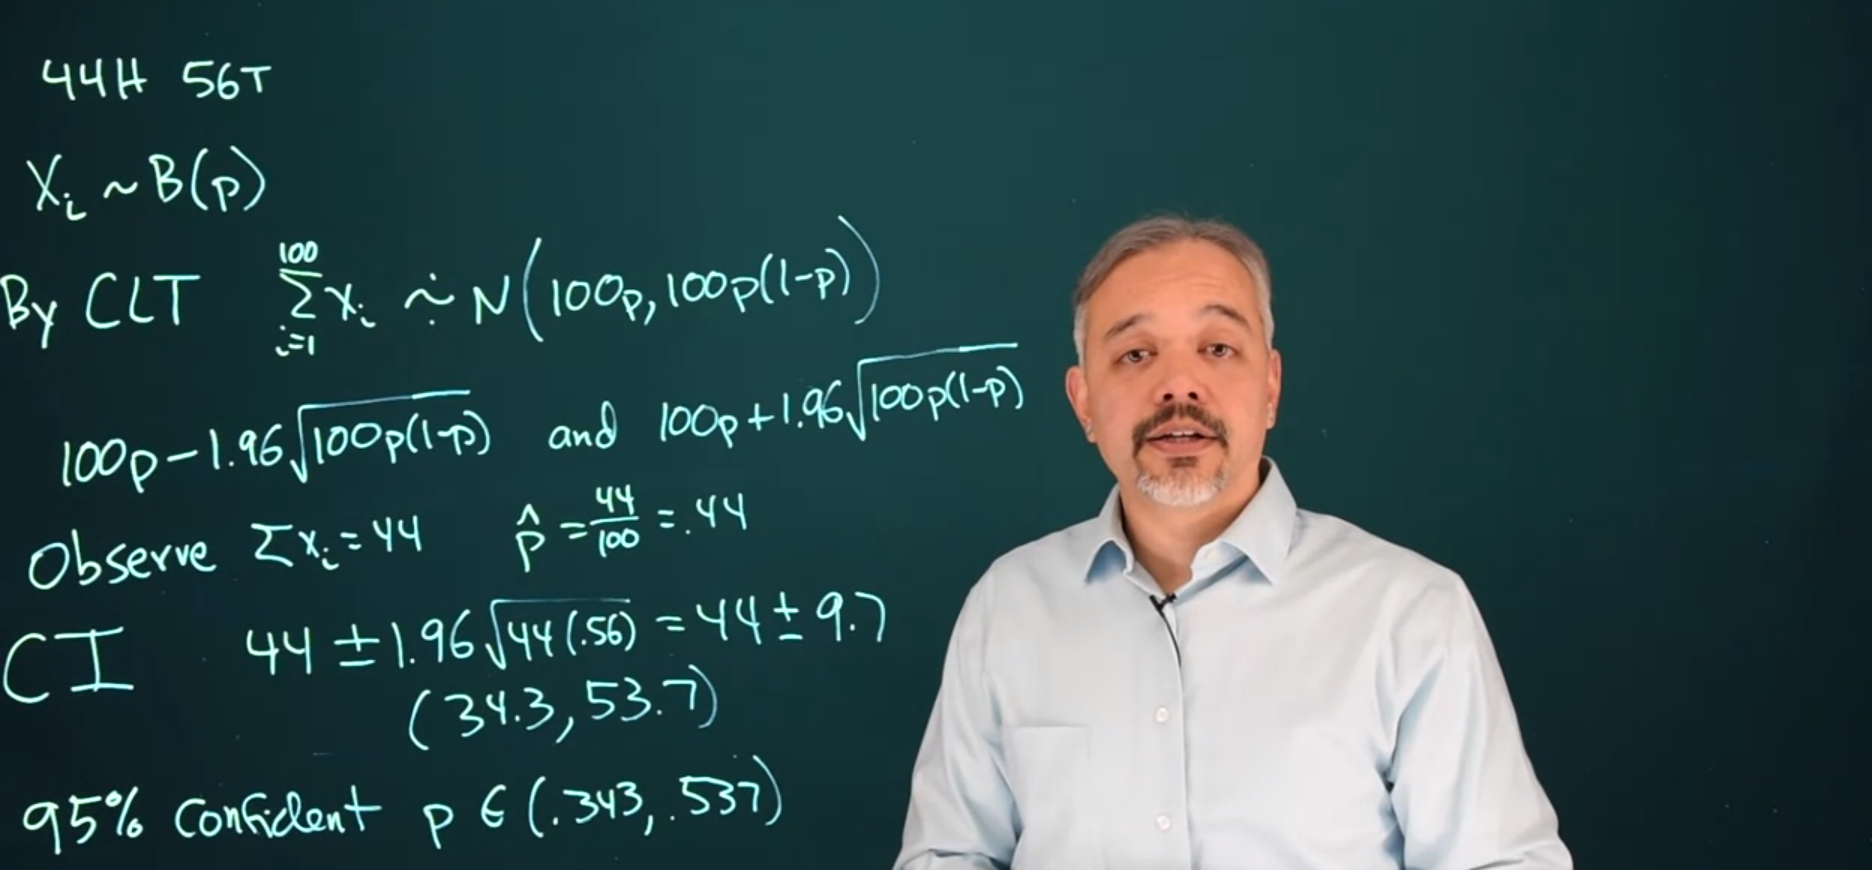
\includegraphics[width=53mm,height=\textheight,keepaspectratio]{images/c1l04-ss-01-confidence-intervals.png}

}

\caption{\label{fig-frequentist-ci}frequentist approach to confidence
intervals}

\end{marginfigure}%

\index{Confidence Interval} A brief review of the frequentist approach
to inference will be useful for contrasting with the Bayesian approach.
(Kruschke 2011) Chapter 2 suggests that CI provides the basis for a
Bayesian workflow and that the rest of the text fills in the missing
pieces.

\begin{tcolorbox}[enhanced jigsaw, bottomrule=.15mm, colbacktitle=quarto-callout-important-color!10!white, leftrule=.75mm, bottomtitle=1mm, titlerule=0mm, title=\textcolor{quarto-callout-important-color}{\faExclamation}\hspace{0.5em}{Frequentist paradigm}, rightrule=.15mm, toprule=.15mm, colback=white, left=2mm, toptitle=1mm, arc=.35mm, opacitybacktitle=0.6, coltitle=black, breakable, opacityback=0, colframe=quarto-callout-important-color-frame]

Under the \textbf{frequentist paradigm}, one views the data as a
\textbf{random sample} from some larger, potentially
\textbf{hypothetical population}. We can then make probability
statements i.e.~\textbf{long-run frequency} statements based on this
larger population.

\end{tcolorbox}

\begin{example}[Coin Flip Example - Central Limit
Theorem]\protect\hypertarget{exm-frequentist-coinflip}{}\label{exm-frequentist-coinflip}

\index{Confidence Interval} \index{Frequentist Inference} Suppose we
flip a coin 100 times. And we get \textbf{44 heads} and \textbf{56
tails}. We can view these 100 flips as a random sample from a much
larger infinite hypothetical population of flips from this coin. We can
say that each flip is \(X_i\) an RV which follows a \emph{Bernoulli
distribution} with some probability \(p\). In this case \(p\) is
unknown, but we can assume it is fixed since we are using a specific
physical coin.

\begin{equation}\phantomsection\label{eq-cointoss-rv}{
X_i \sim B(p)
}\end{equation}

We ask :

\begin{enumerate}
\def\labelenumi{\arabic{enumi}.}
\tightlist
\item
  What is our best estimate of \(p\) the \textbf{probability of getting
  a head}?
\item
  \textbf{How confident are we} in the estimate of \(p\)?
\end{enumerate}

To estimate \(p\) we will apply the \textbf{Central limit theorem} c.f.
\href{@sec-cl-theorem}{Central Limit Theorem} which states that the mean
of a large number of IID RV with mean \(\mu\) and variance \(\sigma^2\)
is approximately \(N(\mu,\sigma^2)\).

\begin{equation}\phantomsection\label{eq-cointoss-clt}{
\sum^{100}_{i=1} X_i\mathrel{\dot \sim } \mathcal{N}(100 \enspace p, 100 \enspace \mathbb{P}r(1-p))
}\end{equation}

\index{Central Limit Theorem} Given that this is a \textbf{Normal
distribution}, we can use the \emph{empirical rule} often called the
\emph{68-95-99.7 rule} see (Wikipedia contributors 2023a), that says
95\% of the time we will get a result is in within 1.96 standard
deviations of the mean. This is referred to as a \emph{Confidence
Interval} or (CI).

\begin{equation}\phantomsection\label{eq-cointoss-ci-theoretical}{
95\% \: \text{CI}= 100 \: \hat{p} \pm 1.96\sqrt{100 \: \hat{p}(1-\hat{p})}
}\end{equation}

Since we observed 44 heads we can estimate \(\hat{p}\) as

\begin{equation}\phantomsection\label{eq-cointoss-phat}{
\hat p = \frac{44}{100} = .44
}\end{equation}

This answers our first questions. Now we want to quantify our
uncertainty.

\begin{equation}\phantomsection\label{eq-cointoss-ci-empirical}{\begin{aligned}
95\% \: \text{CI for 100 tosses} &= 100 \: (.44) \pm 1.96\sqrt{100(0.44)(1-0.44)} \\ 
&= 44 \pm 1.96\sqrt{(44) (0.56)} \\ 
&= 44 \pm 1.96\sqrt{23.64} \\ 
&= (34.27,53.73) \end{aligned}
}\end{equation}

We can be 95\% confident that \(100\times \hat{p} \in [34.3,53.7]\) We
can say that we're 95\% confident that the true probability
\(p \in (.343, .537)\).

If one were to ask \textbf{do I think this coin is \emph{Fair} ?} This
is a reasonable hypothesis, since \(0.5 \in [.343,.537]\).

But we can also step back and say what does this interval mean when we
say we're 95\% confident? Under the frequentist paradigm, we have to
think back to our infinite hypothetical sequence of events, were we to
repeat this trial an arbitrarily large number of times and each time
create a confidence interval, then on average 95\% of the intervals we
make will contain the true value of p.~This makes senses as a long run
frequency explanation.

On the other hand, we might want to know something about this particular
interval. Does this interval contain the true p.~What's the probability
that this interval contains a true p? Well, we don't know for this
particular interval. But under the frequentist paradigm, we're assuming
that there is a fixed right answer for p.~Either p is in that interval
or it's not in that interval. And so technically, from a frequentist
perspective, the probability that p is in this interval is either 0 or
1. This is not a particularly satisfying explanation. In the other hand
when we get to the Bayesian approach we will be able to compute an
interval and actually say there is probably a p is in this interval is
95\% based on a random interpretation of an unknown parameter.

\end{example}

\begin{tcolorbox}[enhanced jigsaw, bottomrule=.15mm, colbacktitle=quarto-callout-tip-color!10!white, leftrule=.75mm, bottomtitle=1mm, titlerule=0mm, title=\textcolor{quarto-callout-tip-color}{\faLightbulb}\hspace{0.5em}{Tip}, rightrule=.15mm, toprule=.15mm, colback=white, left=2mm, toptitle=1mm, arc=.35mm, opacitybacktitle=0.6, coltitle=black, breakable, opacityback=0, colframe=quarto-callout-tip-color-frame]

In this example of flipping a coin 100 times, observing 44 heads
resulted in the following 95\% confidence interval for p: (.343, .537).
From this, we concluded that it is plausible that the coin may be fair
because p=.5 is in the interval.

Suppose instead that we flipped the coin 100,000 times, observing 44,000
heads (the same percentage of heads as before). Then using the method
just presented, the 95\% confidence interval for p is (.437, .443).
\textbf{Is it still reasonable to conclude that this is a fair coin with
95\% confidence}?

\textbf{No} Because \(0.5 \not\in (.437, .443)\), we must conclude that
\(p=.5\) is not a plausible value for the population mean . Observing
100,000 flips increases the power of the experiment, leading to a more
precise estimate with a narrower CI, due to the law of large numbers.

\end{tcolorbox}

\section{Likelihood function and
MLE}\label{sec-likelihood-function-and-MLE}

\begin{marginfigure}

\centering{

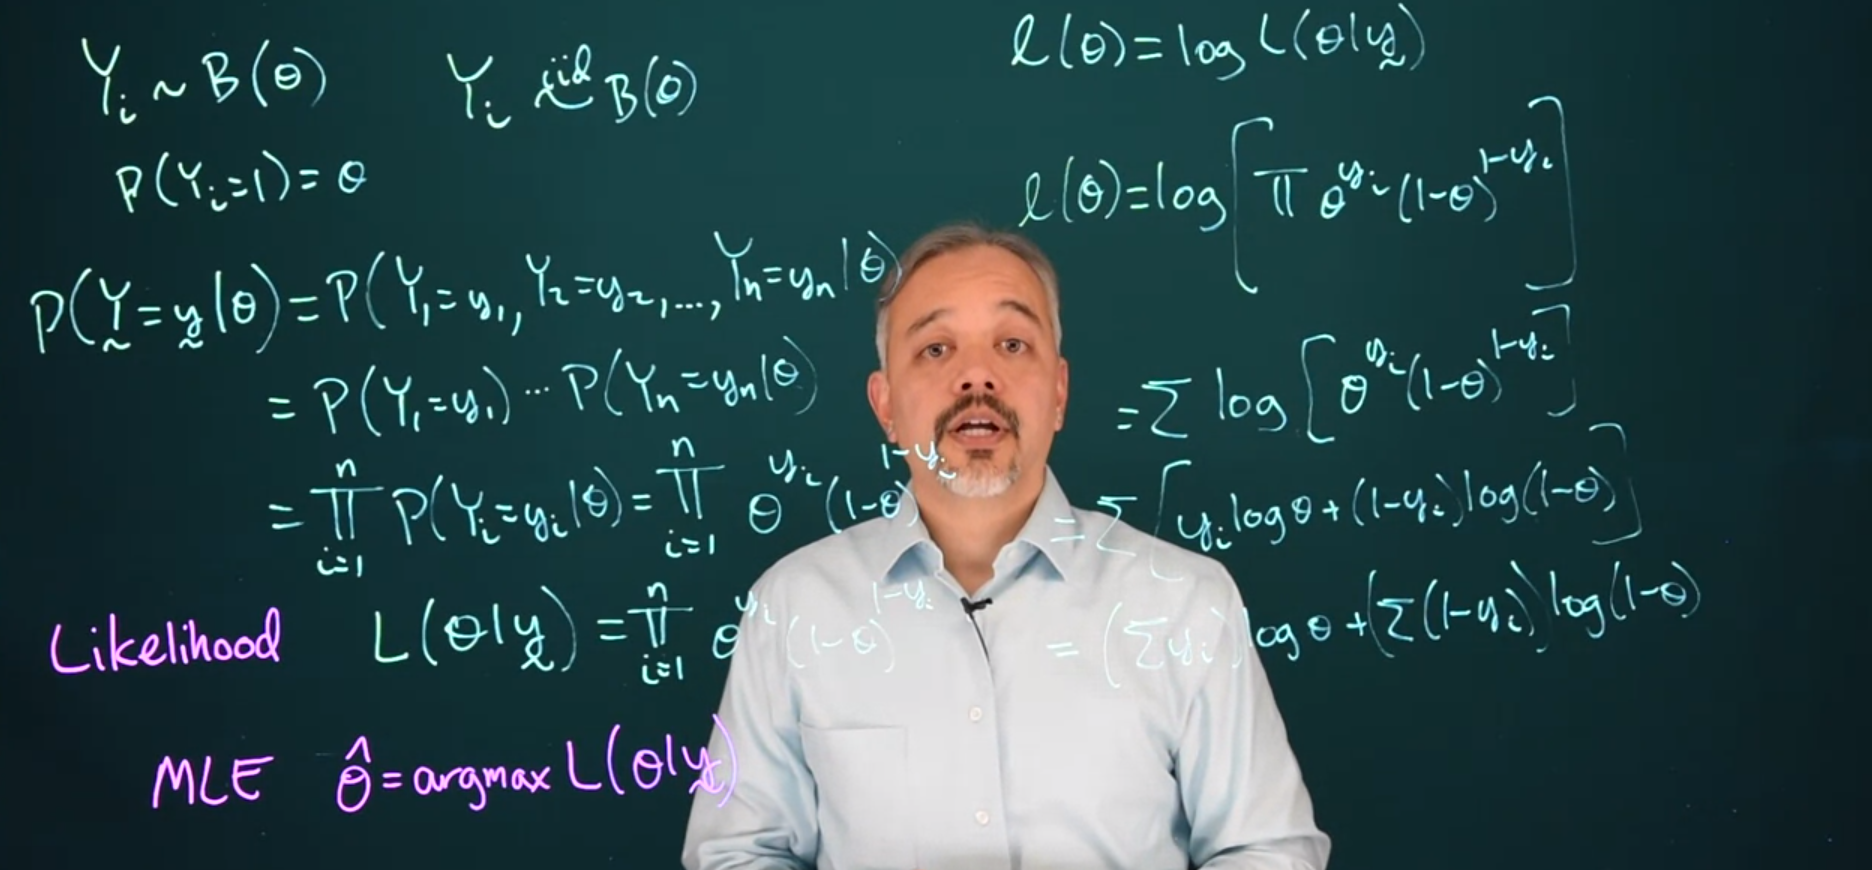
\includegraphics[width=53mm,height=\textheight,keepaspectratio]{images/c1l04-ss-02-Likelihood-fn-and-MLE.png}

}

\caption{\label{fig-likelihood-fn-and-mle}Likelihood fn and MLE}

\end{marginfigure}%

\begin{example}[Heart Attack Patients -
MLE]\protect\hypertarget{exm-frequentist-heartattacks}{}\label{exm-frequentist-heartattacks}

Consider a hospital where 400 patients are admitted over a month for
heart attacks, and a month later 72 of them have died and 328 of them
have survived.

{\marginnote{\begin{footnotesize}\textbf{what's our estimate of the
mortality rate?}\end{footnotesize}}}

\begin{tcolorbox}[enhanced jigsaw, bottomrule=.15mm, colbacktitle=quarto-callout-warning-color!10!white, leftrule=.75mm, bottomtitle=1mm, titlerule=0mm, title=\textcolor{quarto-callout-warning-color}{\faExclamationTriangle}\hspace{0.5em}{Reference Population}, rightrule=.15mm, toprule=.15mm, colback=white, left=2mm, toptitle=1mm, arc=.35mm, opacitybacktitle=0.6, coltitle=black, breakable, opacityback=0, colframe=quarto-callout-warning-color-frame]

Under the \emph{frequentist paradigm}, we must first establish our
\textbf{reference population}. This is the cornerstone of our thinking
as we are considering how the sample parameter approximates the
population statistic. What do we think our reference population is here?

\begin{itemize}
\tightlist
\item
  \textbf{Ref Pop 1}: Heart attack patients in the region.
\item
  \textbf{Ref Pop 2}: Heart attack patients that are admitted to this
  hospital, but over a longer period.
\item
  \textbf{Ref Pop 3}: The people in the region who might have a heart
  attack and might get admitted to this hospital.
\end{itemize}

Both \emph{Ref Pop 1} and \emph{Ref Pop 2} seem like viable options.
Unfortunately, in our data is not a random sample drawn from either. We
could pretend they are and move on, or we could also try to think harder
about what our data is sampled from, perhaps \emph{Ref Pop 3}.

This is an odd hypothetical situation, and so there are some
\emph{philosophical issues} with the setup of this whole problem within
the \emph{frequentist paradigm}

\end{tcolorbox}

\begin{equation}\phantomsection\label{eq-heartattack-rv}{
Y_i \sim \mathrm{Bernoulli}(p)
}\end{equation}

Since this is a Bernoulli trial we need to specify what we interpret as
the \emph{success} . In this case, the \emph{success} is a mortality.

\begin{equation}\phantomsection\label{eq-heartattack-success}{
\mathbb{P}r(Y_i=1) = \theta 
}\end{equation}

The PDF for the dataset can be written in vector form.
\(\mathbb{P}r(\vec{Y}=\vec{y} \mid \theta)\) is the Probability of all
the Y's take some value little y given a value of theta.

\begin{equation}\phantomsection\label{eq-heartattack-pdf}{
\begin{aligned}
\mathbb{P}r(\vec{Y}=\vec{y} \mid \theta) &= \mathbb{P}r(Y_1=y,\dots,Y_n=y_n \mid \theta) && \text{(joint probability)}\\
&= \mathbb{P}r(Y_1=y_1 \mid \theta) \cdots \mathbb{P}r(Y_n=y_n \mid \theta)            && \text {(independence)}\\
&= \prod^n_{i=1} \mathbb{P}r(Y_i=y_i \mid \theta)                            && \text {(product notation)}\\
&= \prod^n_{i=1} \theta^{y_i} (1-\theta)^{1-y_i}                   && \text {(Bernoulli PMF)}
\end{aligned}
}\end{equation}

We now cal the expression for
\(\mathbb{P}r(\vec{Y}=\vec{y} \mid \theta)\) above the likelihood
function \(L(\theta \mid \vec{y} )\):

\begin{equation}\phantomsection\label{eq-heart-attack-likelihood}{  
\mathcal{L}(\theta\mid\vec{y}) = \prod^n_{i=1} \theta^{y_i} (1-\theta)^{1-y_i}
}\end{equation}

Recall that we want to find the mortality rate parameter \(\theta\) for
our Sample \(\vec Y\).

Since it is a probability, it has a range of values from 0 to 1. One way
to estimate it is that there should be one value that maximizes
(Equation~\ref{eq-heart-attack-likelihood}). It makes the data the most
likely to occur for the particular data we observed. This is referred to
as the \textbf{maximum likelihood estimate} (MLE).
\index{Maximum Likelihood Estimation}

\begin{equation}\phantomsection\label{eq-heart-attack-mle}{
\mathop{\mathrm{MLE}}(\hat \theta) = \mathop{\mathrm{argmax}} \; \mathcal{L}(\theta\mid y)
}\end{equation}

Although we are trying to find the \(\theta\) that maximizes the
likelihood, in practice, it's usually easier to maximize the natural
logarithm of the likelihood, commonly referred to as the log-likelihood.

\begin{equation}\phantomsection\label{eq-heart-attack-loglikelihood}{ 
\begin{aligned}
\mathcal{L}(\theta) &= \log(L(\theta|\vec{y}))  && \\
                    &= \log(\prod^n_{i=1} {\theta^{y_i} (1-\theta)^{1-y_i}})       && \text{subst. likelihood} \\
                    &= \sum^n_{i=1}{ \log(\theta^{y_i}) + \log(1-\theta)^{1-y_i}}  && \text{log product rule} \\
                    &= \sum^n_{i=1}{ y_i \log(\theta) + (1-y_i) \log(1-\theta)}     && \text{log power rule}\\
                    &= \log(\theta) \sum^n_{i=1}{  y_i + \log(1-\theta)} \sum^n_{i=1}{  (1-y_i) }& & \text{extracting logs}
\end{aligned}
}\end{equation}

What is the interpretation of the MLE of \(\theta\) in the context of
the heart attack example?

If \(\hat \theta\) is the MLE for \(\theta\), the 30-day mortality rate,
then all possible values of θ produce a lower value of the likelihood
than \(\hat \theta\).

To calculate the MLE one should differentiate \(\mathcal{L}(\theta)\)
w.r.t. \(\theta\) and then set it equal to 0.

\end{example}

\section{Computing the MLE}\label{sec-computing-the-MLE}

\begin{marginfigure}

\centering{

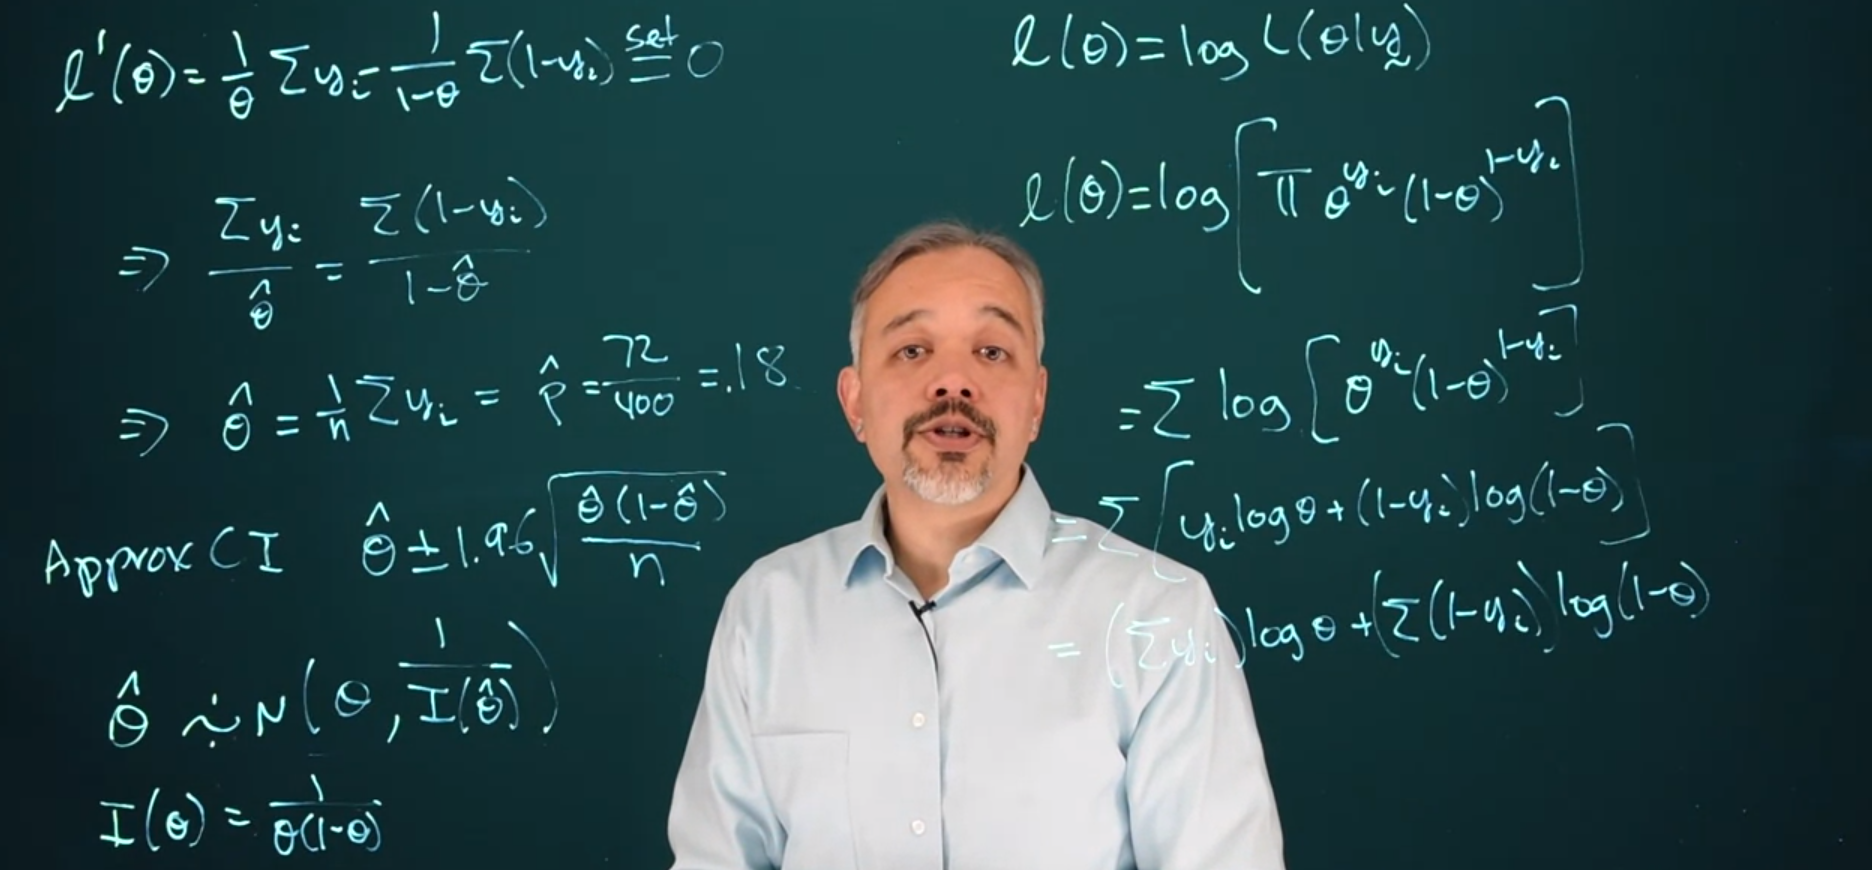
\includegraphics[width=53mm,height=\textheight,keepaspectratio]{images/c1l04-ss-03-computing-the-MLE.png}

}

\caption{\label{fig-computing-the-mle}Computing the MLE}

\end{marginfigure}%

\[
\begin{aligned}
   && \mathcal{L}'(\theta)=& \frac{1}{\theta}\sum_{i=1}^n y_i-\frac{1}{1-\theta}\sum_{i=1}^n 1-y_i \stackrel{\text{set}}{=}0  \text { set derivative to 0}
\\ & \implies   & \frac{1}{\hat \theta}\sum_{i=1}^n y_i & = \frac{1}{1- \hat \theta}\sum_{i=1}^n 1 - y_i 
\\ & \implies   & (1 -\hat \theta) \sum_{i=1}^n{y_i}    &= \hat\theta \sum_{i=1}^n {1-y_i}  
\\ & \implies   & 1 \sum_{i=1}^n{y_i} - \cancel{ \hat \theta \sum_{i=1}^{n}{y_i}} &= \hat\theta \sum_{i=1}^n {1} - \cancel{\hat\theta \sum_{i=1}^n {y_i}}  
\\ & \implies   & \sum_{i=1}^n{y_i}  &= \hat\theta N 
\\ & \implies   &  \hat \theta &= \frac{1}{N} \sum_{i=1}^n y_i  = \hat p = \frac{72}{400}=.18
\end{aligned}
\]

\emph{Maximum Likelihood Estimates} (MLEs) possess the following
favorable properties:

\begin{itemize}
\tightlist
\item
  \textbf{Unbiased} - Thus given sufficient data the MLE will converge
  to the true value. As a consequence, \emph{MLEs are asymptotically
  unbiased}. As we will see in the examples they can still be biased in
  finite samples.
\item
  \textbf{consistent} - One important property of maximum likelihood is
  that it produces consistent estimates.
\item
  \textbf{invariant} - The invariance principle states that the
  \emph{MLE is invariant against reparameterization}.
\end{itemize}

using the Central Limit theorem (see Theorem~\ref{thm-clt}).

\[
\hat \theta \pm 1.96\sqrt\frac{\hat \theta(1-\hat \theta)}{n}
\]

\[
\hat \theta \simeq \mathcal{N}(\theta,\frac{1}{\mathcal{I} (\hat \theta)})
\]

where \(\mathcal{I}\) is the \emph{Fischer information} which for the
Bernoulli distribution is:

\[
\mathcal{I}( \hat \theta) = \frac{1}{\theta(1-\theta)}
\]

Note: The \emph{Fischer information} is a measure of how much
information about theta is in each data point!

\begin{tcolorbox}[enhanced jigsaw, bottomrule=.15mm, colbacktitle=quarto-callout-tip-color!10!white, leftrule=.75mm, bottomtitle=1mm, titlerule=0mm, title=\textcolor{quarto-callout-tip-color}{\faLightbulb}\hspace{0.5em}{Explainable AI (XAI) \& Fischer information}, rightrule=.15mm, toprule=.15mm, colback=white, left=2mm, toptitle=1mm, arc=.35mm, opacitybacktitle=0.6, coltitle=black, breakable, opacityback=0, colframe=quarto-callout-tip-color-frame]

In XAI we use discuss local and global explanations.

\begin{itemize}
\tightlist
\item
  \texttt{Global\ explanations} explain a black box model's predictions
  based on each feature, via its parameters.
\item
  \texttt{Local\ explanations} explain the prediction of a specific
  datum from its features.
\end{itemize}

since \texttt{Fischer\ information} quantifies the information in a data
point on a parameter we should be able to use it to produce local and
perhaps even global explanations for Bayesian models.

\end{tcolorbox}

\section{Computing the MLE:
examples}\label{sec-computing-the-MLE-examples}

Some more examples of maximum likelihood estimators.

\subsection{Computing the MLE for Exponential
RV}\label{sec-computing-the-MLE-for-exponential-RV}

\begin{marginfigure}

\centering{

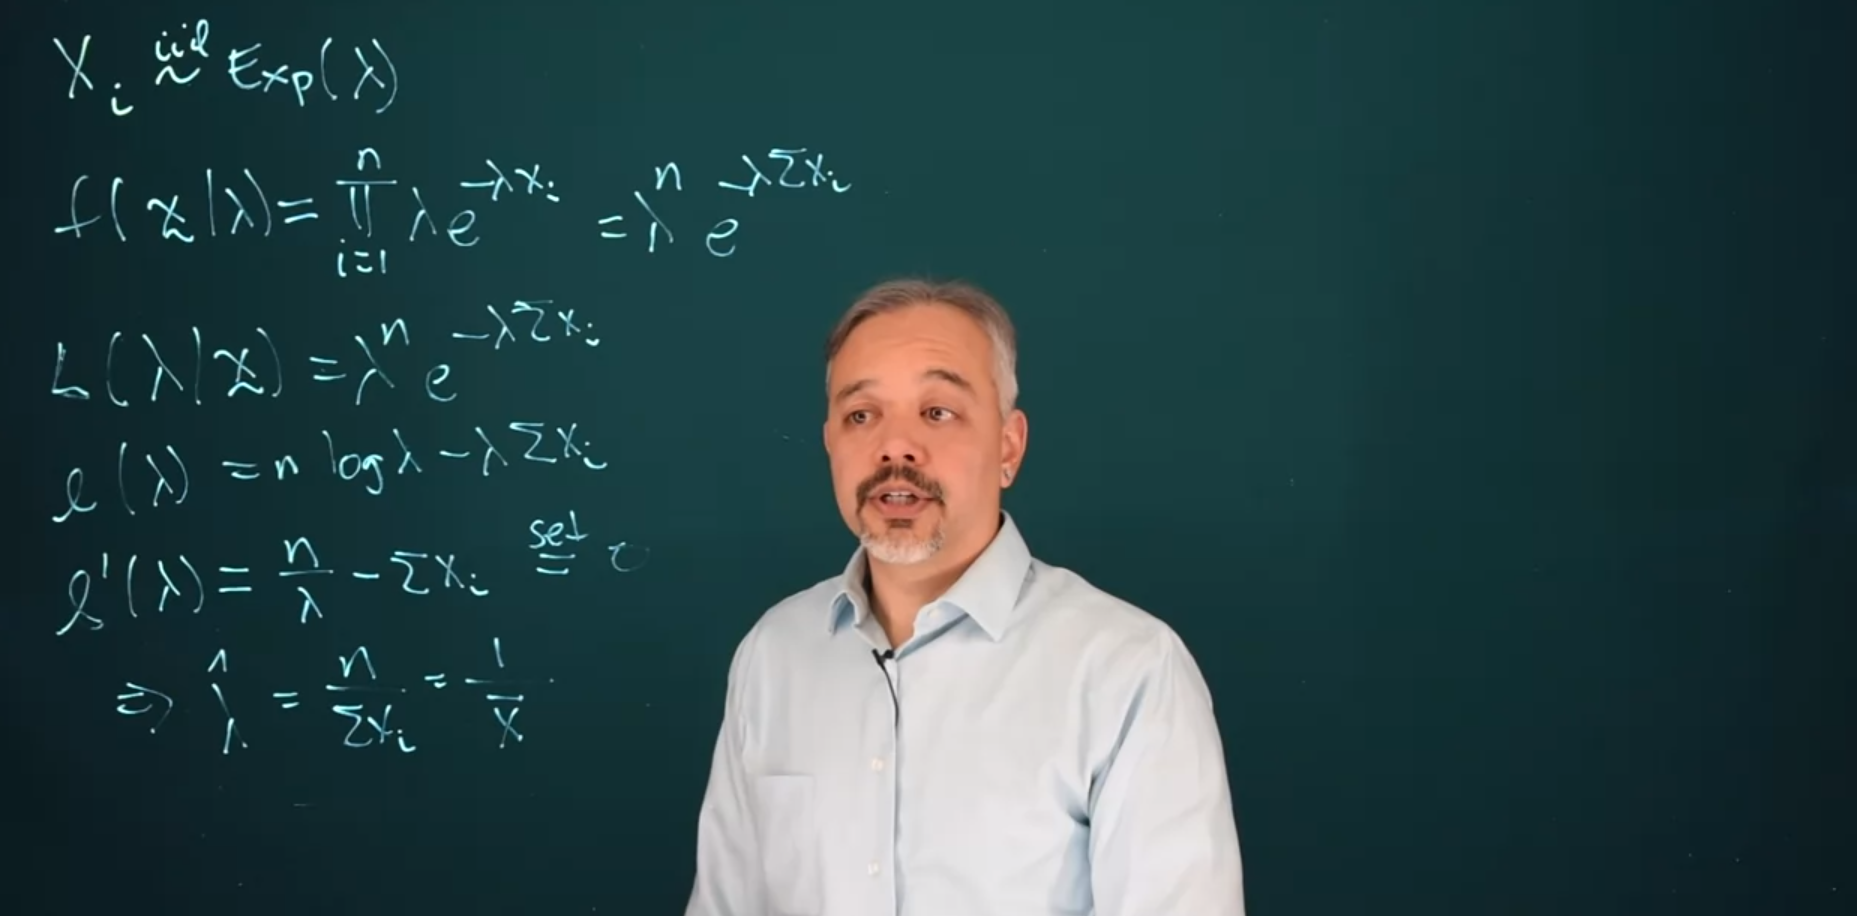
\includegraphics[width=53mm,height=\textheight,keepaspectratio]{images/c1l04-ss-04-computing-the-exponential-MLE.png}

}

\caption{\label{fig-computing-the-MLE-for-exponential-rv}computing the
MLE for Exponential RV}

\end{marginfigure}%

Let's say \(X_i\) are exponential distributed

\[ 
X_i \sim \mathrm{Exp}(\lambda) 
\]

Let's say the data is independent and identically distributed, therefore
making the overall density function

\begin{equation}\phantomsection\label{eq-exp-likelihood-derivation}{
\begin{aligned}
  f(x \mid \lambda) &= \prod_{i = 1}^n{\lambda e^{-\lambda x_i}} && \text {(simplifying)} \\
                    &= \lambda^ne^{-\lambda \sum{x_i}}
\end{aligned}
}\end{equation}

Now the likelihood function is

\begin{equation}\phantomsection\label{eq-exp-likelihood-fn}{
\mathcal{L}(\lambda \mid x)=\lambda^ne^{-\lambda \sum{x_i}}
}\end{equation}

the log likelihood is

\begin{equation}\phantomsection\label{eq-exp-log-likelihood-fn}{
\ell(\lambda) = n\ln{\lambda} - \lambda\sum_i{x_i}
}\end{equation}

Taking the derivative

\begin{equation}\phantomsection\label{eq-exp-log-likelihood-derivative}{
\begin{aligned}
  \ell^\prime(\lambda) &= \frac{n}{\lambda} - \sum_i{x_i} \stackrel{\text{set}}{=}0 && \text {(set derivative = 0)} \\ 
  \implies \frac{n}{\hat{\lambda}} &= \sum_i{x_i} && \text{(rearranging)}
\end{aligned}
}\end{equation}

\begin{equation}\phantomsection\label{eq-exp-MLE}{
\hat{\lambda} = \frac{n}{\sum_i{x_i}} = \frac{1}{\bar{x}}
}\end{equation}

\subsection{Computing the MLE for Uniform
RV}\label{sec-computing-the-MLE-for-uniform-RV}

\begin{marginfigure}

\centering{

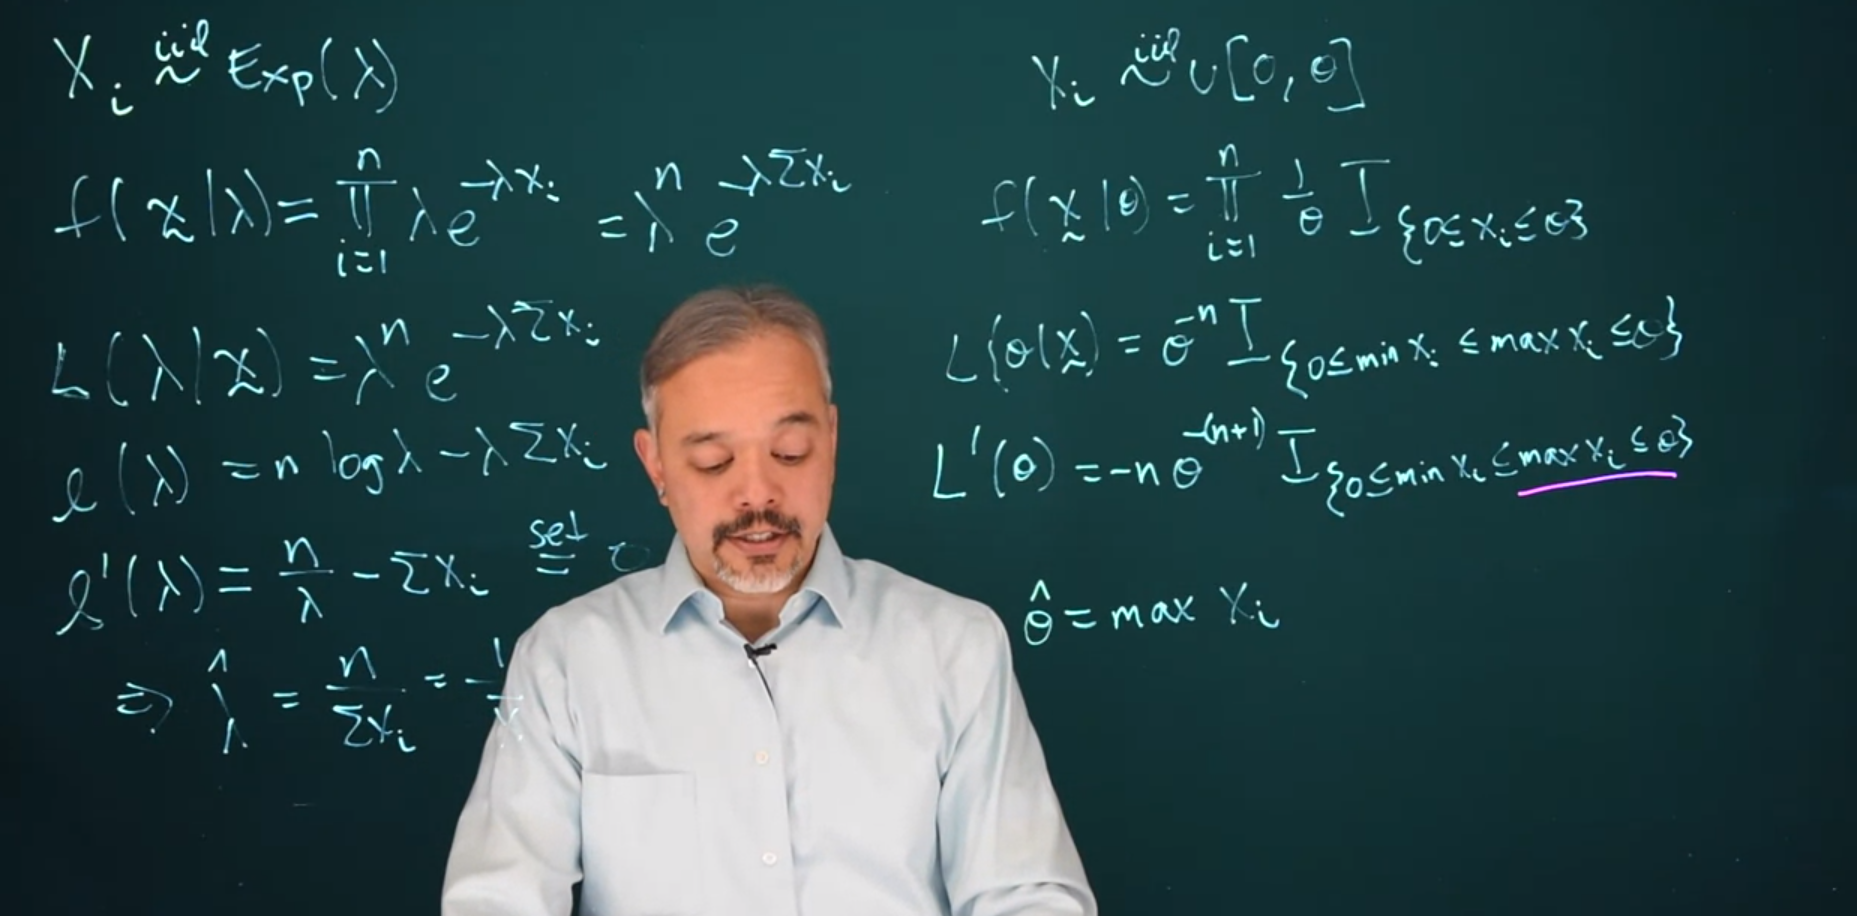
\includegraphics[width=53mm,height=\textheight,keepaspectratio]{images/c1l04-ss-05-computing-the-uniform-MLE.png}

}

\caption{\label{fig-computing-the-MLE-for-uniform-RV}computing the MLE
for Uniform RV}

\end{marginfigure}%

\begin{equation}\phantomsection\label{eq-uniform-mle-rv}{
X_i \sim \mathcal{U}[0, \theta]
}\end{equation}

\begin{equation}\phantomsection\label{eq-uniform-MLE-likelihood-derivation}{
f(x \mid \theta) = \prod_{i = 1}^n{\frac{1}{\theta}\mathbb{I}_{0 \le x_i \le \theta}}
}\end{equation}

Combining all the indicator functions, for this to be a 1, each of these
has to be true. These are going to be true if all the observations are
bigger than 0, as in the minimum of the x is bigger than or equal to 0.
The maximum of the x's is also less than or equal to \(\theta\).

\begin{equation}\phantomsection\label{eq-uniform-MLE-likelihood}{
\mathcal{L}(\theta|x) = \theta^{-1} \mathbb{I}_{0\le min(x_i) \le max(x_i) \le \theta}
}\end{equation}

\begin{equation}\phantomsection\label{eq-uniform-MLE-likelihood-derivative}{
\mathcal{L}^\prime(\theta) = -n\theta^{-(n + 1)}\mathbb{I}_{0 \le min(x_i) \le max(x_i)\le \theta}
}\end{equation}

We ask, can we set this equal to zero and solve for \(\theta\)? It turns
out, this is not equal to zero for any \(\theta\) positive value. We
need \(\theta\) to be strictly larger than zero. But for \(\theta\)
positive, this will always be negative. The derivative is negative, that
says this is a decreasing function. Therefore this function will be
maximized when we pick \(\theta\) as small as possible. What's the
smallest possible value of \(\theta\) we can pick? Well we need in
particular for \(\theta\) to be larger than all of the \(X_i\). And so,
the maximum likelihood estimate is the maximum of \(X_i\)

\begin{equation}\phantomsection\label{eq-uniform-mle}{
\hat{\theta} = max(x_i)
}\end{equation}

\section{Cumulative Distribution
Function}\label{sec-cumulative-distribution-function}

The cumulative distribution function (CDF) exists for every
distribution. We define it as \(F(x) = \mathbb{P}r(X \le x)\) for random
variable \(X\).

If \(X\) is discrete-valued, then the CDF is computed with summation
\(F(x) = \sum_{t = -\infty}^x {f(t)}\). where
\(f(t) = \mathbb{P}r(X = t)\) is the probability mass function (PMF)
which we've already seen.

If \(X\) is continuous, the CDF is computed with an integral
\(F(x) = \int_{-\infty}^x{f(t)dt}\)

The CDF is convenient for calculating probabilities of intervals. Let
\(a\) and \(b\) be any real numbers with \(a < b\). Then the probability
that \(X\) falls between \(a\) and \(b\) is equal to
\(\mathbb{P}r(a < X < b) = \mathbb{P}r(X \le b) - \mathbb{P}r(X \le a) = F(b) - F(a)\)

\begin{figure}

\centering{

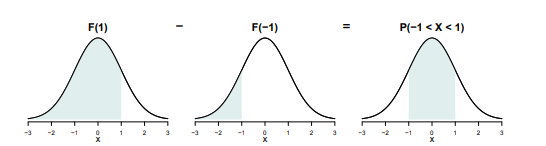
\includegraphics[width=53mm,height=\textheight,keepaspectratio]{images/c1l04-ss-06-CDF.png}

}

\caption{\label{fig-interval-from-cdf}Illustration of using the CDF to
calculate the probability of an interval for continuous random variable
X. Probability values are represented with shaded regions in the
graphs.}

\end{figure}%

\begin{example}[CDF example
1]\protect\hypertarget{exm-cdf-1}{}\label{exm-cdf-1}

Suppose \(X \sim \mathrm{Binomial}(5, 0.6)\). Then

\begin{equation}\phantomsection\label{eq-cdf-ex1}{
  \begin{aligned}
  F(1) &= \mathbb{P}r(X \le 1) 
\\ &= \sum_{−∞}^1 f(t) 
\\ &= \sum_{t=−∞}^{-1} 0 + \sum_{t=0}^1 {5 \choose t} 0.6^t (1 − 0.6)^{5−t} 
\\ &= {5 \choose 0} 0.6^0 (1 − 0.6)5−0 +{5 \choose 1} 0.6^1 (1 − 0.6)^{5−1} 
\\ &= (0.4)^5 + 5(0.6)(0.4)^4
\\ &≈ 0.087
\end{aligned}
}\end{equation}

\end{example}

\begin{example}[CDF example
1]\protect\hypertarget{exm-cdf-2}{}\label{exm-cdf-2}

Example: Suppose \(Y ∼ Exp(1)\). Then

\begin{equation}\phantomsection\label{eq-cdf-ex2}{
\begin{aligned}
F(2) &= \mathbb{P}r(Y \le 2) 
\\ &= \int^{2}_{−∞} e^{−t}\mathbb{I}_{(t≥0)} dt 
\\ &= \int^{2}_{0} e^{−t}dt 
\\ &= −e^{−t}|^2_0 
\\ &= −(e^{−2} − e^0) 
\\ &= 1−e^{−2} 
\\ &\approx 0.865
\end{aligned}
}\end{equation}

\end{example}

\section{Quantile Function}\label{sec-quantile-function}

The CDF takes a value for a random variable and returns a probability.
Suppose instead we start with a number between \(0\) and \(1\), which we
call \(p\), and we wish to find a value \(x\) so that
\(\mathbb{P}r(X \le x) = p\). The value \(x\) which satisfies this
equation is called the \(p\) quantile. (or \(100p\) percentile) of the
distribution of \(X\).

\begin{example}[Quantile Function example
1]\protect\hypertarget{exm-qf-1}{}\label{exm-qf-1}

In a standardized test, the 97th percentile of scores among all
test-takers is 23. Then 23 is the score you must achieve on the test in
order to score higher than 97\% of all test-takers. We could
equivalently call \(q = 23\) the .97 quantile of the distribution of
test scores.

\end{example}

\begin{example}[Quantile Function example
2]\protect\hypertarget{exm-qf-2}{}\label{exm-qf-2}

The middle 50\% of probability mass for a continuous random variable is
found between the .25 and .75 quantiles of its distribution. If
\(Z \sim N(0, 1)\), then the \(.25\) quantile is \(−0.674\) and the
\(.75\) quantile is 0.674. Therefore,
\(\mathbb{P}r(−0.674 <Z <0.674) = 0.5\).

\end{example}

\chapter{Introduction to R}\label{sec-introduction-to-r}

R has some nice functions that one can use for analysis

\texttt{mean(z)} gives the mean of some row vector \(z\)

\texttt{var(z)} reports the variance of some row vector

\texttt{sqrt(var(z))} gives the standard deviation of some row vector

\texttt{seq(from=0.1,\ to\ =\ 0.9,\ by\ =\ 0.1)} creates a vector that
starts from \(0.1\) and goes to \(0.9\) incrementing by \(0.1\)

\begin{Shaded}
\begin{Highlighting}[]
\FunctionTok{seq}\NormalTok{(}\AttributeTok{from=}\FloatTok{0.1}\NormalTok{, }\AttributeTok{to =} \FloatTok{0.9}\NormalTok{, }\AttributeTok{by =} \FloatTok{0.1}\NormalTok{)}
\end{Highlighting}
\end{Shaded}

\begin{verbatim}
[1] 0.1 0.2 0.3 0.4 0.5 0.6 0.7 0.8 0.9
\end{verbatim}

\begin{Shaded}
\begin{Highlighting}[]
\FunctionTok{seq}\NormalTok{(}\DecValTok{1}\NormalTok{, }\DecValTok{10}\NormalTok{)}
\end{Highlighting}
\end{Shaded}

\begin{verbatim}
 [1]  1  2  3  4  5  6  7  8  9 10
\end{verbatim}

\texttt{names(x)} gives the names of all the columns in the dataset.

\begin{Shaded}
\begin{Highlighting}[]
\FunctionTok{names}\NormalTok{(trees)}
\end{Highlighting}
\end{Shaded}

\begin{verbatim}
[1] "Girth"  "Height" "Volume"
\end{verbatim}

\texttt{hist(x)} provides a histogram based on a vector

The more general \texttt{plot} function tries to guess at which type of
plot to make. Feeding it two numerical vectors will make a scatter plot.

The R function \texttt{pairs} takes in a data frame and tries to make
all possible Pairwise scatterplots for the dataset.

The \texttt{summary} command gives the five/six number summary (minimum,
first quartile, median, mean, third quartile, maximum)

\section{Plotting the likelihood function in
R}\label{sec-plotting-the-likelihood-function-in-r}

Going back to the hospital example

\begin{Shaded}
\begin{Highlighting}[]
\NormalTok{likelihood }\OtherTok{=} \ControlFlowTok{function}\NormalTok{(n, y, theta) \{}
  \FunctionTok{return}\NormalTok{(theta}\SpecialCharTok{\^{}}\NormalTok{y }\SpecialCharTok{*}\NormalTok{ (}\DecValTok{1} \SpecialCharTok{{-}}\NormalTok{ theta)}\SpecialCharTok{\^{}}\NormalTok{(n }\SpecialCharTok{{-}}\NormalTok{ y))}
\NormalTok{\}}
\NormalTok{theta }\OtherTok{=} \FunctionTok{seq}\NormalTok{(}\AttributeTok{from =} \FloatTok{0.01}\NormalTok{, }\AttributeTok{to =} \FloatTok{0.99}\NormalTok{, }\AttributeTok{by =} \FloatTok{0.01}\NormalTok{)}
\FunctionTok{plot}\NormalTok{(theta, }\FunctionTok{likelihood}\NormalTok{(}\DecValTok{400}\NormalTok{, }\DecValTok{72}\NormalTok{, theta))}
\end{Highlighting}
\end{Shaded}

\pandocbounded{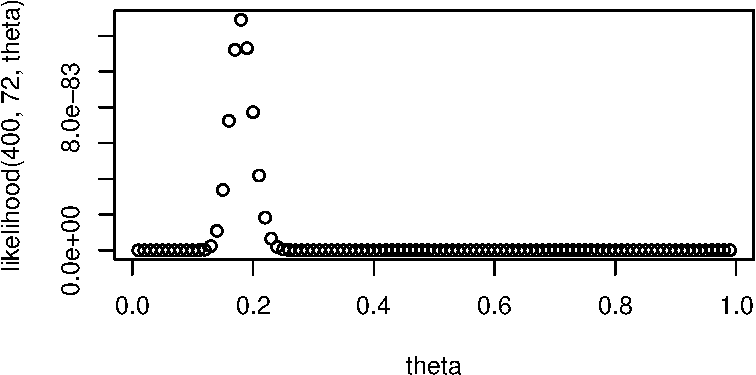
\includegraphics[keepaspectratio]{C1-L04_files/figure-pdf/intro-likelihood-function-1.pdf}}

You can also do this with log likelihoods. This is typically more
numerically stable to compute

\begin{Shaded}
\begin{Highlighting}[]
\NormalTok{loglike }\OtherTok{=} \ControlFlowTok{function}\NormalTok{(n, y, theta) \{}
  \FunctionTok{return}\NormalTok{(y }\SpecialCharTok{*} \FunctionTok{log}\NormalTok{(theta) }\SpecialCharTok{+}\NormalTok{ (n }\SpecialCharTok{{-}}\NormalTok{ y) }\SpecialCharTok{*} \FunctionTok{log}\NormalTok{(}\DecValTok{1} \SpecialCharTok{{-}}\NormalTok{ theta))}
\NormalTok{\}}
\FunctionTok{plot}\NormalTok{(theta, }\FunctionTok{loglike}\NormalTok{(}\DecValTok{400}\NormalTok{, }\DecValTok{72}\NormalTok{, theta))}
\end{Highlighting}
\end{Shaded}

\pandocbounded{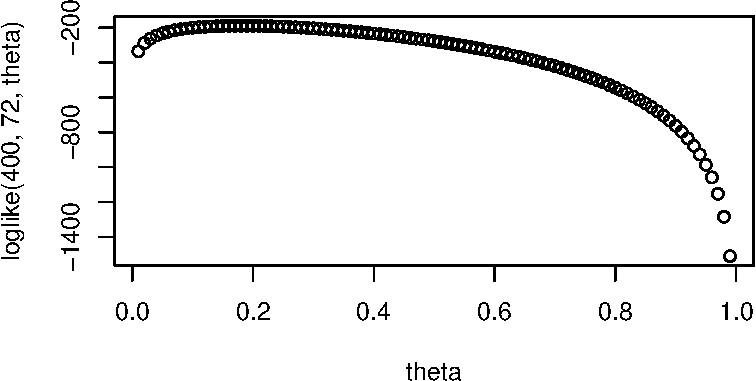
\includegraphics[keepaspectratio]{C1-L04_files/figure-pdf/intro-loglikelihood-function-plot1-1.pdf}}

Having these plotted as points makes it difficult to see, let's plot it
as lines

\begin{Shaded}
\begin{Highlighting}[]
\FunctionTok{plot}\NormalTok{(theta, }\FunctionTok{loglike}\NormalTok{(}\DecValTok{400}\NormalTok{, }\DecValTok{72}\NormalTok{, theta), }\AttributeTok{type =} \StringTok{"l"}\NormalTok{)}
\end{Highlighting}
\end{Shaded}

\pandocbounded{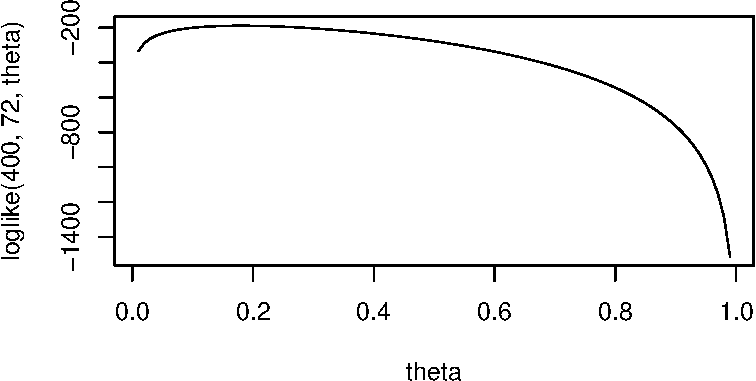
\includegraphics[keepaspectratio]{C1-L04_files/figure-pdf/intro-likelihood-function-plot2-1.pdf}}

\chapter{Probability Distributions in
R}\label{sec-probability-distributions-in-r}

Each of the distributions introduced in Lesson 3 have convenient
functions in R which allow you to evaluate the PDF/PMF, CDF, and
quantile functions, as well as generate random samples from the
distribution. To illustrate, see Table~\ref{tbl-r-api-normal}, which
lists these functions for the normal distribution

\begin{longtable}[]{@{}
  >{\raggedright\arraybackslash}p{(\linewidth - 2\tabcolsep) * \real{0.2472}}
  >{\raggedright\arraybackslash}p{(\linewidth - 2\tabcolsep) * \real{0.7528}}@{}}
\caption{R API for the normal
distribution}\label{tbl-r-api-normal}\tabularnewline
\toprule\noalign{}
\begin{minipage}[b]{\linewidth}\raggedright
Function
\end{minipage} & \begin{minipage}[b]{\linewidth}\raggedright
What it does
\end{minipage} \\
\midrule\noalign{}
\endfirsthead
\toprule\noalign{}
\begin{minipage}[b]{\linewidth}\raggedright
Function
\end{minipage} & \begin{minipage}[b]{\linewidth}\raggedright
What it does
\end{minipage} \\
\midrule\noalign{}
\endhead
\bottomrule\noalign{}
\endlastfoot
\texttt{dnorm(x,\ mean,\ sd)} & Evaluate the PDF at \(x\) (mean =
\(\mu\) and sd = \(\sqrt{\sigma^2}\)) \\
\texttt{pnorm(q,\ mean,\ sd)} & Evaluate the CDF at \(q\) \\
\texttt{qnorm(p,\ mean,\ sd)} & Evaluate the quantile function at
\(p\) \\
\texttt{rnorm(n,\ mean,\ sd)} & Generate \(n\) pseudo-random samples
from the normal distribution \\
\end{longtable}

These four functions exist for each distribution where \texttt{d...}
function evaluates the density/mass, \texttt{p...} evaluates the CDF,
\texttt{q...} evaluates the quantile, and \texttt{r...} generates a
sample. In Table~\ref{tbl-r-api-distributions} which lists the
\texttt{d...} functions for some of the most popular distributions. The
\texttt{d} can be replaced with \texttt{p}, \texttt{q}, or \texttt{r}
for any of the distributions, depending on what you want to calculate.

For details enter \texttt{?dnorm} to view R's documentation page for the
Normal distribution. As usual , replace the \texttt{norm} with any
distribution to read the documentation for that distribution.

\begin{longtable}[]{@{}
  >{\raggedright\arraybackslash}p{(\linewidth - 4\tabcolsep) * \real{0.2667}}
  >{\raggedright\arraybackslash}p{(\linewidth - 4\tabcolsep) * \real{0.3111}}
  >{\raggedright\arraybackslash}p{(\linewidth - 4\tabcolsep) * \real{0.4222}}@{}}
\caption{R API for
distribution}\label{tbl-r-api-distributions}\tabularnewline
\toprule\noalign{}
\begin{minipage}[b]{\linewidth}\raggedright
Distribution
\end{minipage} & \begin{minipage}[b]{\linewidth}\raggedright
Function
\end{minipage} & \begin{minipage}[b]{\linewidth}\raggedright
Parameters
\end{minipage} \\
\midrule\noalign{}
\endfirsthead
\toprule\noalign{}
\begin{minipage}[b]{\linewidth}\raggedright
Distribution
\end{minipage} & \begin{minipage}[b]{\linewidth}\raggedright
Function
\end{minipage} & \begin{minipage}[b]{\linewidth}\raggedright
Parameters
\end{minipage} \\
\midrule\noalign{}
\endhead
\bottomrule\noalign{}
\endlastfoot
\(Binomial(n,p)\) & \texttt{dbinom(x,\ size,\ prob)} & size = \(n\),
prob = \(p\) \\
\(Poisson(\lambda)\) & \texttt{dpois(x,\ lambda)} & lambda =
\(\lambda\) \\
\(Exp(\lambda)\) & \texttt{dexp(x,\ rate)} & rate = \(\lambda\) \\
\(Gamma(\alpha, \beta)\) & \texttt{dgamma(x,\ shape,\ rate)} & shape =
\(\alpha\), rate = \(\beta\) \\
\(Uniform(a, b)\) & \texttt{dunif(x,\ min,\ max)} & min = \(a\), max =
\(b\) \\
\(Beta(\alpha, \beta)\) & \texttt{dbeta(x,\ shape1,\ shape2)} & shape1 =
\(\alpha\), shape2 = \(\beta\) \\
\(N(\mu, \sigma^2)\) & \texttt{dnorm(x,\ mean,\ sd)} & mean = \(\mu\),
sd = \(\sqrt{\sigma^2}\) \\
\(t_v\) & \texttt{dt(x,\ df)} & df = \(v\) \\
\end{longtable}

\chapter{Frequentist MLE - M2L3HW1}\label{frequentist-mle---m2l3hw1}

Bayesian Statistics: From Concept to Data Analysis

\hfill\break

\begin{tcolorbox}[enhanced jigsaw, bottomrule=.15mm, colbacktitle=quarto-callout-caution-color!10!white, leftrule=.75mm, bottomtitle=1mm, titlerule=0mm, title=\textcolor{quarto-callout-caution-color}{\faFire}\hspace{0.5em}{Caution}, rightrule=.15mm, toprule=.15mm, colback=white, left=2mm, toptitle=1mm, arc=.35mm, opacitybacktitle=0.6, coltitle=black, breakable, opacityback=0, colframe=quarto-callout-caution-color-frame]

Section omitted to comply with the Honor Code

\end{tcolorbox}

\chapter{Bayesian Inference - M2L5}\label{bayesian-inference---m2l5}

Bayesian Statistics: From Concept to Data Analysis

\hfill\break

\section{Inference example:
frequentist}\label{sec-inference-example-frequentist}

\begin{marginfigure}

\centering{

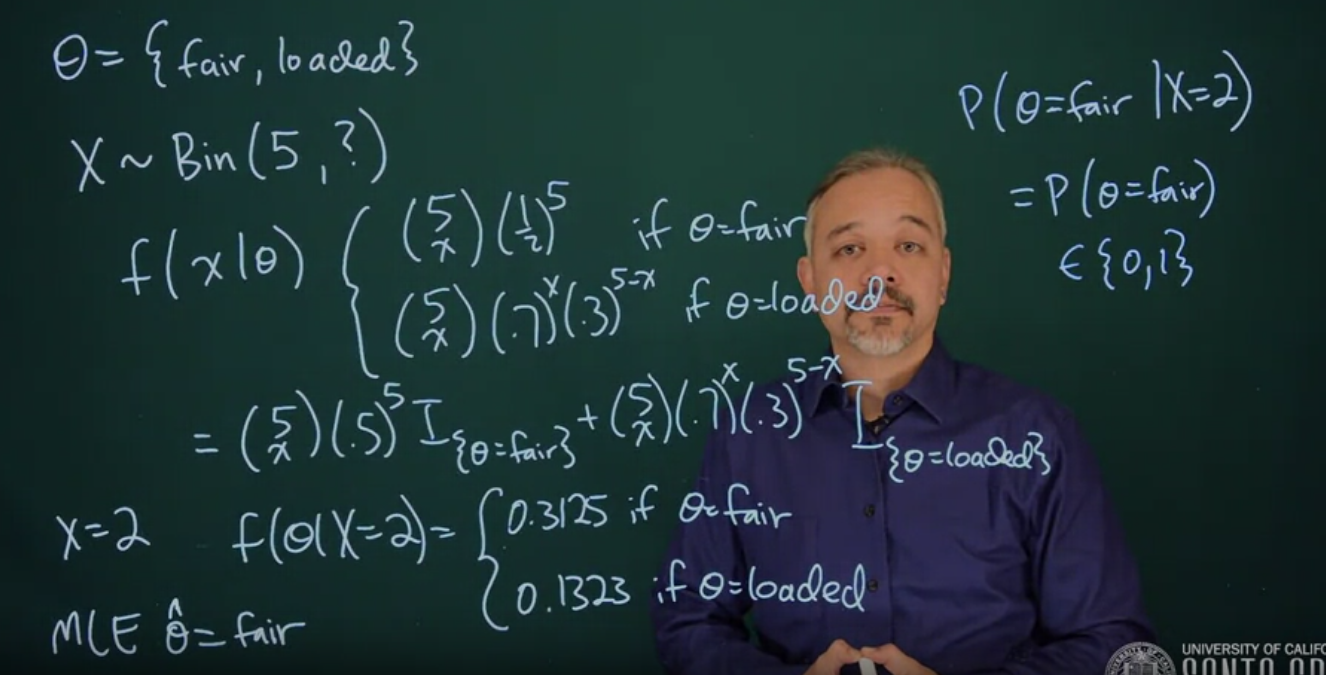
\includegraphics[width=53mm,height=\textheight,keepaspectratio]{images/c1l05-ss-01-inference-example-frequentist.png}

}

\caption{\label{fig-coin-probability-inference}coin probability
inference}

\end{marginfigure}%

\begin{example}[Two Coin
Example]\protect\hypertarget{exm-two-coins}{}\label{exm-two-coins}

Suppose your brother has a coin that you know to be loaded so that it
comes up heads 70\% of the time. He then comes to you with some coin,
you're not sure which one and he wants to make a bet with you. Betting
money that it's going to come up heads.

You're not sure if it's the loaded coin or if it's just a fair one. So
he gives you a chance to flip it 5 times to check it out.

You flip it five times and get 2 heads and 3 tails.

{\marginnote{\begin{footnotesize}\textbf{Which coin do you think it is
and how sure are you about that?}\end{footnotesize}}}

\end{example}

We'll start by defining the unknown parameter \(\theta\), this is either
that the coin is fair or it's a loaded coin.

\begin{equation}\phantomsection\label{eq-two-coins-parameter}{
\theta = \{\text{fair},\ \text{loaded}\} \qquad \text{(parameter)}
}\end{equation}

we get to flip it five times but we do not know what kind of coin it is

\begin{equation}\phantomsection\label{eq-two-coins-model}{
X \sim Bin(5, \theta) \qquad \text{(model)}
}\end{equation}

each value of theta gives us a competing binomial likelihood:

\begin{equation}\phantomsection\label{eq-two-coins-likelihood}{
f(x\ mid\theta) = 
    \begin{cases} 
      {5 \choose x}(\frac{1}{2})^5            & \theta = \text{fair} \\
      {5 \choose x} (.7)^x (.3)^{5 - x}       & \theta = \text{loaded}
   \end{cases} 
   \qquad \text{(likelihood)}
}\end{equation}

We can also rewrite the likelihood \(f(x \mid \theta)\) using indicator
functions

\begin{equation}\phantomsection\label{eq-two-coins-likelihood-indicator}{
f(x\mid\theta) = {5\choose x}(.5)^5\mathbb{I}_{\{\theta= \text{fair}\}} + {5 \choose x}(.7)^x(.3)^{5 - x}\mathbb{I}_{\{\theta = \text{loaded}\}} \qquad \text{(likelihood)}
}\end{equation}

In this case, we observed that \(x = 2\)

\begin{equation}\phantomsection\label{eq-two-coins-likelihood-sub-x}{
f(\theta \mid x = 2) = 
    \begin{cases} 
        0.3125 & \theta = \text{fair} \\
        0.1323 & \theta = \text{loaded}
    \end{cases} 
    \qquad \text{(sub. x=2)}
}\end{equation}

\begin{equation}\phantomsection\label{eq-two-coins-MLE}{
\therefore \hat{\theta} = \text{fair} MLE
}\end{equation}

That's a good point estimate, but then how do we answer the question,
\emph{how sure are you}?

This is not a question that's easily answered in the frequentest
paradigm. Another question is that we might like to know what is the
probability that theta equals fair, give, we observe two heads.

\begin{equation}\phantomsection\label{eq-two-coins-certainty}{
\mathbb{P}r(\theta = \text{fair} \mid x = 2) = ?
}\end{equation}

In the \emph{frequentest paradigm}, the coin is a physical quantity.
It's a fixed coin, and therefore it has a fixed probability of coining
up heads. It is either the fair coin, or it's the loaded coin.

\[
\mathbb{P}r(\theta = \text{fair}) = \{0,1\}
\]

\section{Bayesian Approach to the
Problem}\label{sec-bayesian-approach-to-the-problem}

\begin{marginfigure}

\centering{

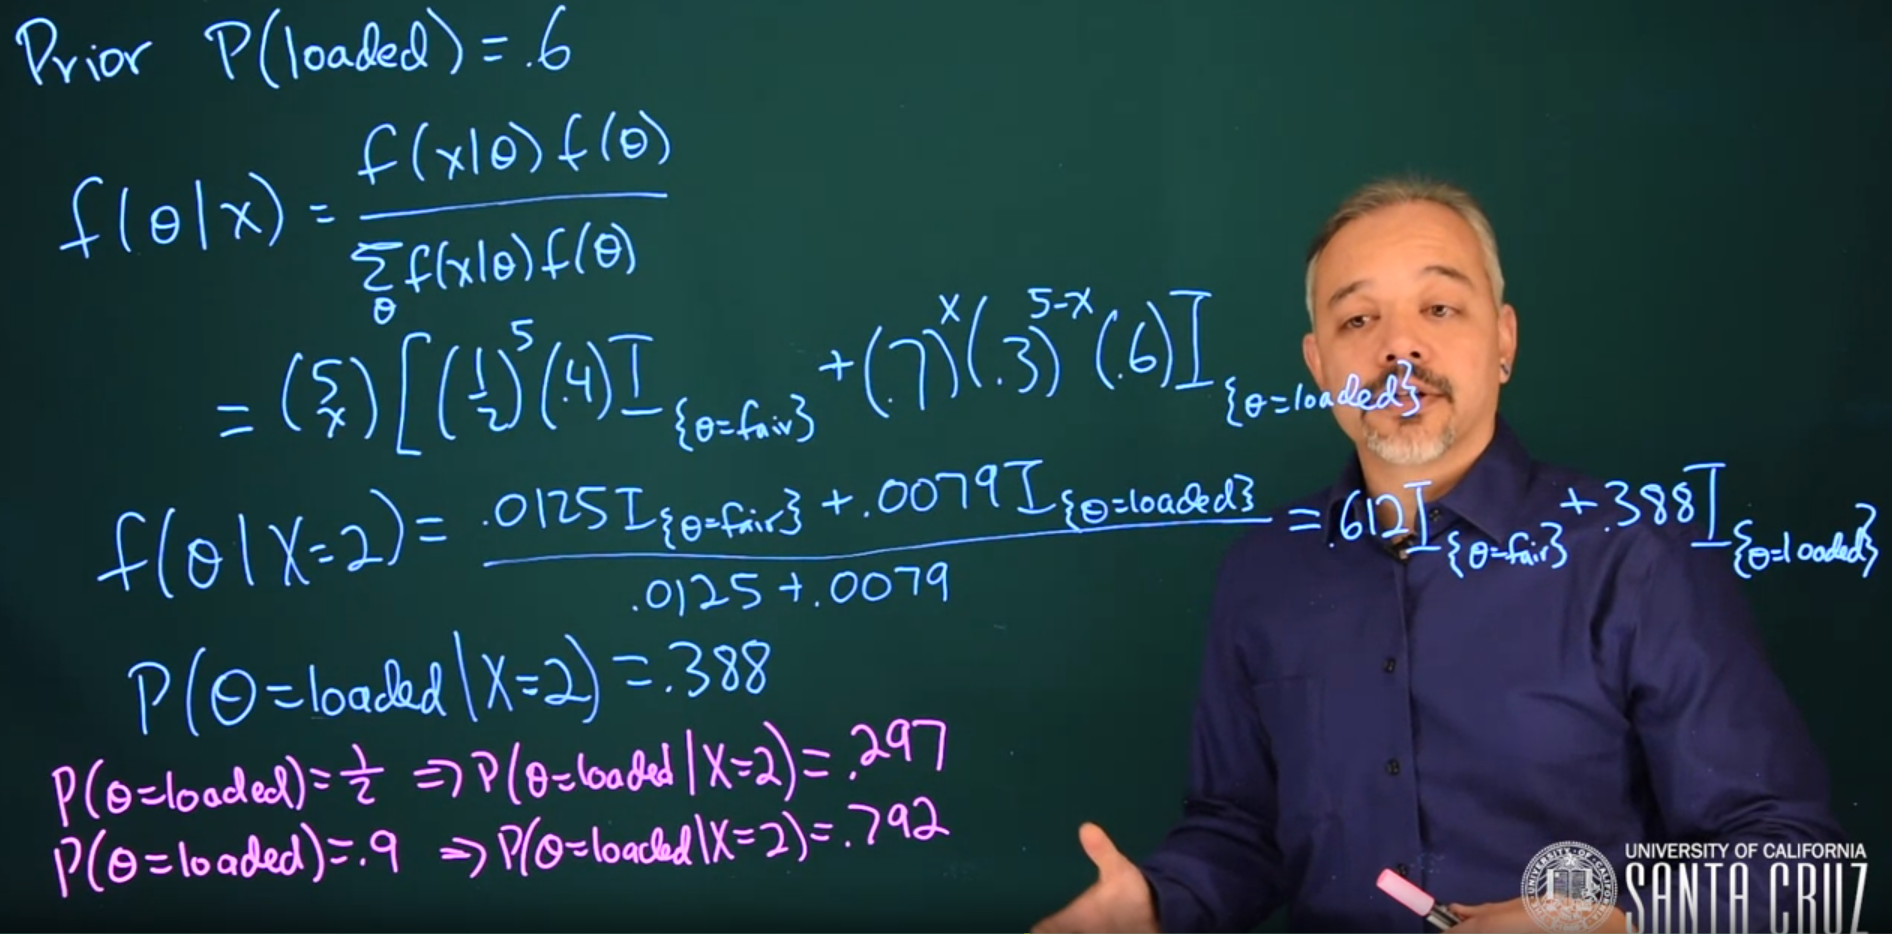
\includegraphics[width=53mm,height=\textheight,keepaspectratio]{images/c1l05-ss-02-inference-example-bayesian.png}

}

\caption{\label{fig-bayesian-coin-probability-inference}Bayesian coin
probability inference}

\end{marginfigure}%

An advantage of the Bayesian approach is that it allows you to easily
incorporate prior information when you know something in advance of
looking at the data. This is difficult to do under the \emph{frequentist
paradigm}.

In this case, we're talking about your brother. You probably know him
pretty well. So suppose you think that before you've looked at the coin,
there's a 60\% probability that this is the loaded coin.

In this case, we put this into our prior. Our prior belief is that the
probability the coin is loaded is 0.6. We can update our prior beliefs
with the data to get our posterior beliefs, and we can do this using the
\emph{Bayes theorem}.

\begin{equation}\phantomsection\label{eq-inference}{
\begin{aligned}
  \mathbb{P}r(\text{loaded}) &= 0.6\ && \text{(prior)}
\\ f(\theta \mid x) &= \frac{f(x \mid \theta)f(\theta)}{\sum_\theta{f(x \mid \theta)f(\theta)}} && \text{(Bayes)}
\\ f(\theta\mid x=2)&= \frac{{5\choose x} \left [(\frac{1}{2})^5(1-0.6)\ \mathbb{I}_{(\theta = \text{fair})} + (.7)^x (.3)^{5-x}(.6)\ \mathbb{I}_{(\theta = \text{loaded})}  \right] } {{5\choose x} \left [(\frac{1}{2})^5(.4) + (.7)^x (.3)^{5-x}(0.6)  \right] }&& \text{(sub. x=2)}
\\ &= \frac{0.0125\ \mathbb{I}_{(\theta = \text{fair})}  + 0.0079\ \mathbb{I}_{(\theta = \text{loaded})} }{0.0125+0.0079}&& \text{(normalize)}
\\ &= \textbf{0.612}\ \mathbb{I}_{(\theta=\text{fair})} + 0.388\ \mathbb{I}_{(\theta = \text{loaded})} && \text{(MLE)} 
\end{aligned}
}\end{equation}

As you can see in the calculation Equation~\ref{eq-inference}, we have
the \emph{likelihood} times the \emph{prior} in the numerator, and a
\emph{normalizing constant} in the denominator. When we divide the two,
we'll get an answer that adds up to 1. These numbers match exactly in
this case because it's a very simple problem.

This is a concept that we will revisit --- what's in the denominator
here is always a normalizing constant.

\[ 
\mathbb{P}r(\theta = loaded \mid x = 2) = 0.388 
\]

This here updates our beliefs after seeing some data about what the
probability might be.

We can also examine what would happen under different choices of prior.

\[
\mathbb{P}r(\theta = loaded) = \frac{1}{2} \implies \mathbb{P}r(\theta = loaded \mid x = 2) = 0.297 
\]

\[
\mathbb{P}r(\theta = loaded) = 0.9 \implies \mathbb{P}r(\theta = loaded \mid x = 2) = 0.792
\]

In this case, the Bayesian approach is inherently subjective. It
represents your perspective, and this is an important part of the
paradigm. If you have a different perspective, you will get different
answers, and that's okay. It's all done in a mathematically vigorous
framework, and it's all mathematically consistent and coherent.

And in the end, we get interpretable results.

\section{Continuous version of Bayes'
theorem}\label{sec-continuous-version-of-bayes-theorem}

\begin{marginfigure}

\centering{

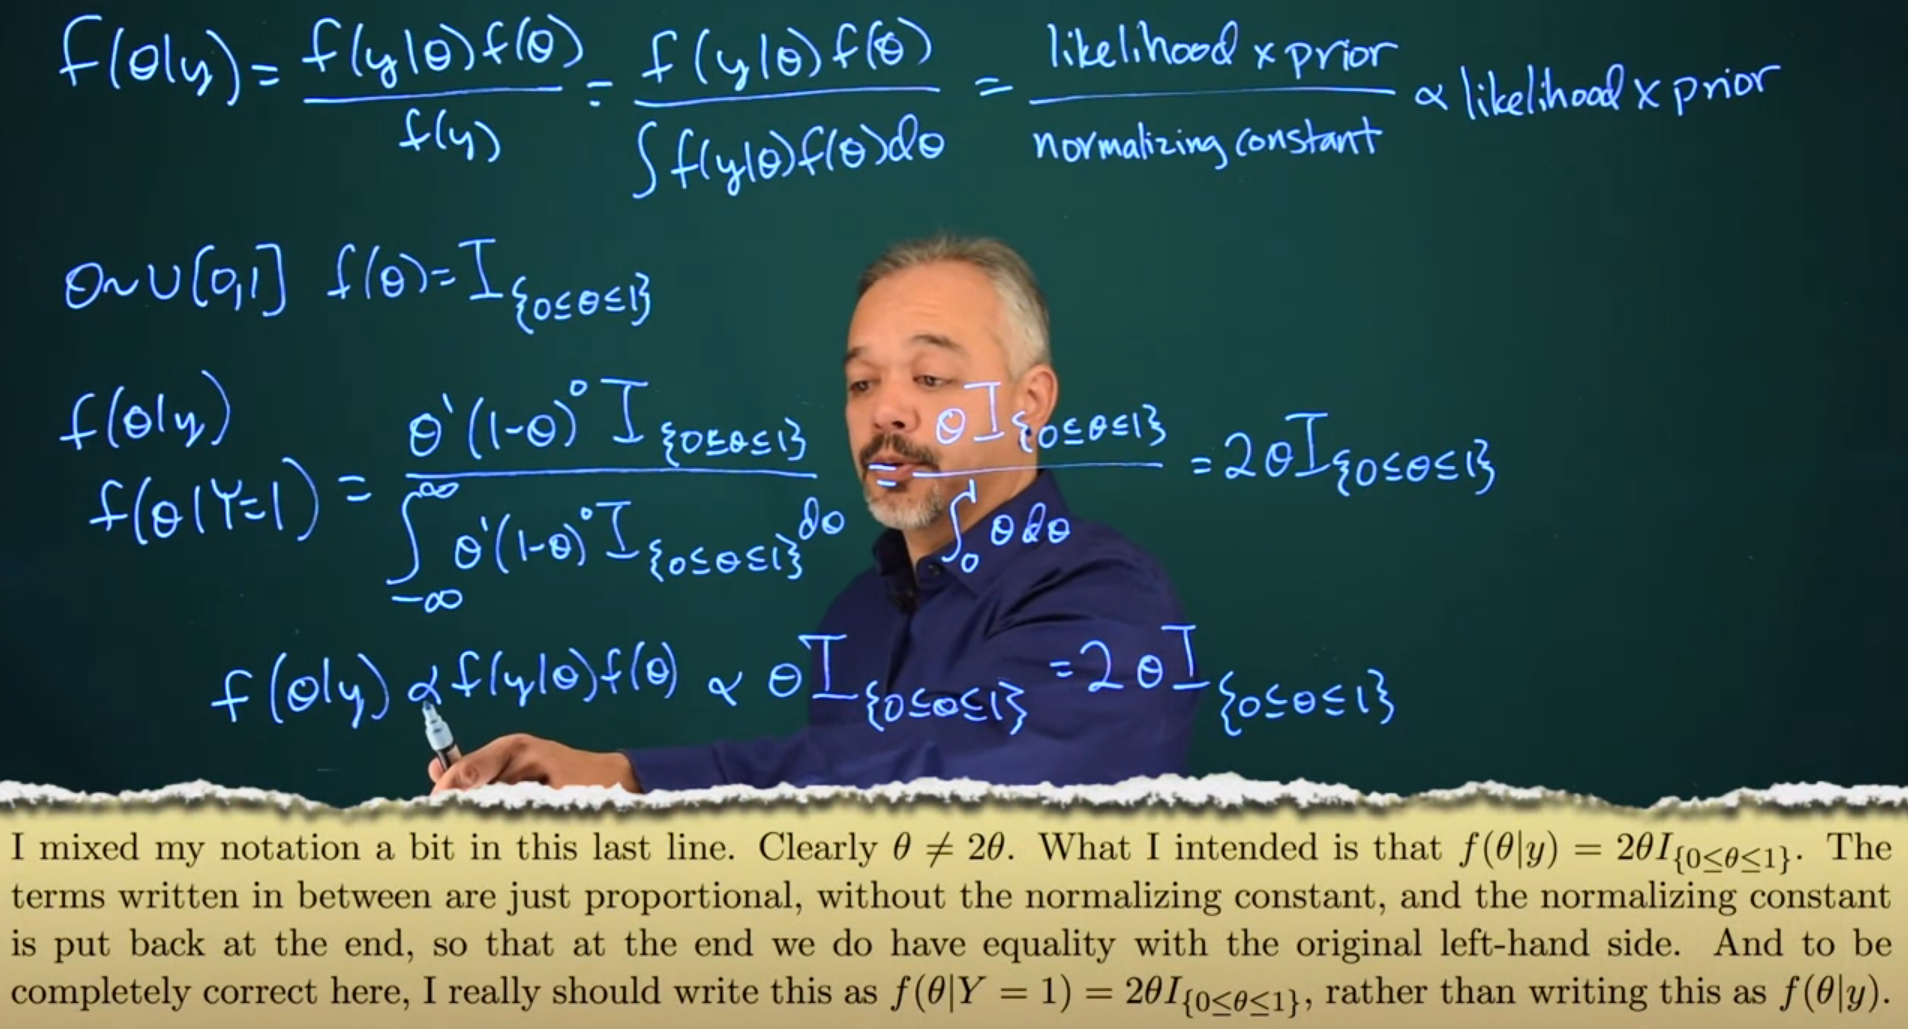
\includegraphics[width=53mm,height=\textheight,keepaspectratio]{images/c1l05-ss-03-continuous-bayes-theorem.png}

}

\caption{\label{fig-continuous-bayes-theorem}Continuous version of
Bayes' theorem}

\end{marginfigure}%

\section{Posterior Intervals}\label{sec-posterior-intervals}

\begin{marginfigure}

\centering{

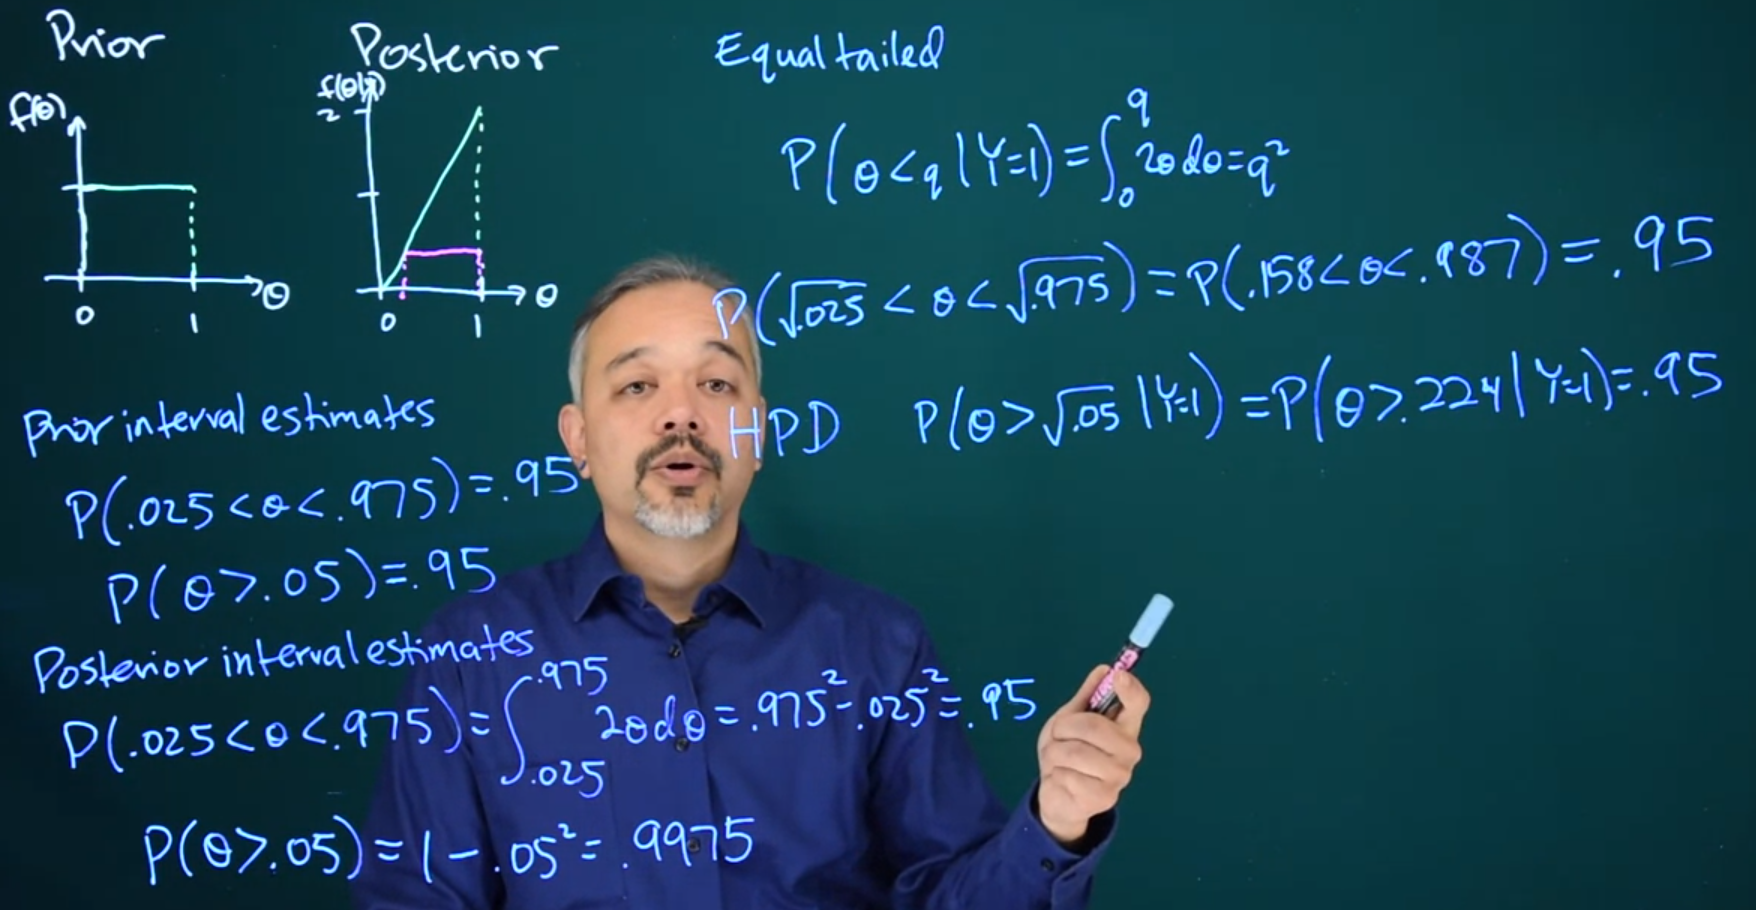
\includegraphics[width=53mm,height=\textheight,keepaspectratio]{images/c1l05-ss-04-posterior-intervals.png}

}

\caption{\label{fig-posterior-intervals}Posterior Intervals}

\end{marginfigure}%

\section{Discussion CIs}\label{sec-discussion-cis}

\begin{itemize}
\tightlist
\item
  \textbf{Frequentist confidence intervals} have the interpretation that
  ``If you were to repeat many times the process of collecting data and
  computing a 95\% confidence interval, then on average about 95\% of
  those intervals would contain the true parameter value; however, once
  you observe data and compute an interval the true value is either in
  the interval or it is not, but you can't tell which.''
\item
  \textbf{Bayesian credible intervals} have the interpretation that
  ``Your posterior probability that the \emph{parameter} is in a 95\%
  credible interval is 95\%.''
\item
  Bayesian intervals treat their bounds as fixed and the estimated
  parameter as a random variable.
\item
  Frequentist confidence intervals treat their bounds as random
  variables and the parameter as a fixed value.
\end{itemize}

\begin{tcolorbox}[enhanced jigsaw, bottomrule=.15mm, colbacktitle=quarto-callout-note-color!10!white, leftrule=.75mm, bottomtitle=1mm, titlerule=0mm, title=\textcolor{quarto-callout-note-color}{\faInfo}\hspace{0.5em}{Discussion Under what circumstances would you prefer a frequentist CI or
a Bayesian CI?}, rightrule=.15mm, toprule=.15mm, colback=white, left=2mm, toptitle=1mm, arc=.35mm, opacitybacktitle=0.6, coltitle=black, breakable, opacityback=0, colframe=quarto-callout-note-color-frame]

\subsection{Focusing on Bayesian / Frequentist
paradigms}\label{focusing-on-bayesian-frequentist-paradigms}

\begin{itemize}
\tightlist
\item
  A Frequentist CI might be preferred if:

  \begin{enumerate}
  \def\labelenumi{\arabic{enumi}.}
  \tightlist
  \item
    I had plenty of data to support a frequentist construction of
    frequentist CI and
  \item
    I was doing research and refining or refuting a result that has been
    established using frequentist hypothesis testing.

    \begin{itemize}
    \tightlist
    \item
      I would want to show that for \(H_1\) against some null
      hypothesis, \(H_0\) the parameters have a certain p-value for some
      effect.
    \item
      Particularly when we are interested in the inference and are less
      interested in using the value of the parameter.
    \end{itemize}
  \item
    I cannot justify introducing some subjective priors.
  \end{enumerate}
\item
  A Bayesian CI might be better if:

  \begin{enumerate}
  \def\labelenumi{\arabic{enumi}.}
  \tightlist
  \item
    My dataset is too small.
  \item
    What I care about is the parameter's value and less about hypothesis
    testing
  \item
    I need an estimate of uncertainty for the parameter for the
    inference it is used in.
  \item
    I had subjective reasons to introduce a prior:

    \begin{itemize}
    \tightlist
    \item
      I know about constraints
    \item
      I have access to expert knowledge
    \end{itemize}
  \item
    I wish to introduce pooling between groups, to share information for
    reducing uncertainty.
  \item
    My results are in a Bayesian-oriented domain.
  \end{enumerate}
\end{itemize}

\end{tcolorbox}

\begin{tcolorbox}[enhanced jigsaw, bottomrule=.15mm, colbacktitle=quarto-callout-note-color!10!white, leftrule=.75mm, bottomtitle=1mm, titlerule=0mm, title=\textcolor{quarto-callout-note-color}{\faInfo}\hspace{0.5em}{Discussion: Under what circumstances would you prefer a frequentist CI
or a Bayesian CI?}, rightrule=.15mm, toprule=.15mm, colback=white, left=2mm, toptitle=1mm, arc=.35mm, opacitybacktitle=0.6, coltitle=black, breakable, opacityback=0, colframe=quarto-callout-note-color-frame]

\subsection{Focusing on the CI
choices}\label{focusing-on-the-ci-choices}

Let's point out that this is what we call a loaded question, as it has a
bias against the frequentist approach by stating one of its shortcomings
when it is still possible to get a point estimate for the parameter and
compare it to the CI. Typically one will have already done it say using
regression before considering the CI.

Next, we have all the standard reasons for choosing between the
Frequentist and the Bayesian paradigms. I could list them but I don't
think that is the real point of this question, but rather what would we
prefer if both were viable options and why?

CIs are primarily a tool for understanding uncertainties about
parameters that encode effects. In the parametric Bayesian approach we
are learning the distribution of our parameters so they have
uncertainties baked into them. In the Frequentist approach, we look for
the least squares point estimates for our parameters and consider using
the CI to approximate the long-run uncertainty due to sampling.

Frequentist CI might be preferable if I am worried about Aletoric
uncertainty due to sampling i.e.~to what degree can I be certain my
experimental outcomes are not due to chance? I would feel this way since
I am a classical physicist or a botanist studying a predominately
deterministic effect and I see errors in estimating the parameters as
artifacts of sampling that can be made smaller till the parameters will
converge with the true population statistics and the error will become
vanishingly small.

Given that I did my best to get a good data sample I just need to check
how sure to decide the cardinal question do I publish or do I perish? I
need to decide that the result is due to the effect and not due to some
conspiracy bad samples.

Bayesian CIs are just a result of using Bayesian analysis which is a
requirement to investigate what are predominately random effects that
are the domain of quantum physicists, an ecologist, or a geneticist.
Since almost everything I study is predominantly random and I need
random variables and Bayes law to get to my results. I also need to
report confidence intervals for my work when I publish - but if one is a
Bayesian, one will use a Bayesian credible interval?

\end{tcolorbox}

\chapter{Homework on Likelihoods and MLEs -
M2L5HW1}\label{homework-on-likelihoods-and-mles---m2l5hw1}

Bayesian Statistics: From Concept to Data Analysis

\hfill\break

\begin{tcolorbox}[enhanced jigsaw, bottomrule=.15mm, colbacktitle=quarto-callout-caution-color!10!white, leftrule=.75mm, bottomtitle=1mm, titlerule=0mm, title=\textcolor{quarto-callout-caution-color}{\faFire}\hspace{0.5em}{Caution}, rightrule=.15mm, toprule=.15mm, colback=white, left=2mm, toptitle=1mm, arc=.35mm, opacitybacktitle=0.6, coltitle=black, breakable, opacityback=0, colframe=quarto-callout-caution-color-frame]

Section omitted to comply with the Honor Code

\end{tcolorbox}

\chapter{Homework on Bayesian Inference -
M2L5HW2}\label{homework-on-bayesian-inference---m2l5hw2}

Bayesian Statistics: From Concept to Data Analysis

\hfill\break

\begin{tcolorbox}[enhanced jigsaw, bottomrule=.15mm, colbacktitle=quarto-callout-caution-color!10!white, leftrule=.75mm, bottomtitle=1mm, titlerule=0mm, title=\textcolor{quarto-callout-caution-color}{\faFire}\hspace{0.5em}{Caution}, rightrule=.15mm, toprule=.15mm, colback=white, left=2mm, toptitle=1mm, arc=.35mm, opacitybacktitle=0.6, coltitle=black, breakable, opacityback=0, colframe=quarto-callout-caution-color-frame]

Section omitted to comply with the Honor Code

\end{tcolorbox}

\chapter{Priors - M3L6}\label{priors---m3l6}

Bayesian Statistics: From Concept to Data Analysis

\hfill\break

In this section, we will delve more deeply into choices of Priors and
how they influence Bayesian CI by developing the \textbf{prior
predictive} (Definition~\ref{def-prior-predictive-distribution}) and
posterior \textbf{predictive}
(Definition~\ref{def-posterior-predictive-distribution}) intervals.

\section{Priors and prior predictive
distributions}\label{sec-priors-and-prior-predictive-distributions}

\begin{tcolorbox}[enhanced jigsaw, bottomrule=.15mm, colbacktitle=quarto-callout-important-color!10!white, leftrule=.75mm, bottomtitle=1mm, titlerule=0mm, title=\textcolor{quarto-callout-important-color}{\faExclamation}\hspace{0.5em}{Choosing a prior}, rightrule=.15mm, toprule=.15mm, colback=white, left=2mm, toptitle=1mm, arc=.35mm, opacitybacktitle=0.6, coltitle=black, breakable, opacityback=0, colframe=quarto-callout-important-color-frame]

\textbf{How should we choose a prior?}

\begin{enumerate}
\def\labelenumi{\arabic{enumi}.}
\tightlist
\item
  Our prior needs to represent our perspectives, beliefs, and our
  uncertainties.
\item
  It should encode any constraints on the data or parameters.

  \begin{itemize}
  \tightlist
  \item
    age is positive and less than 120
  \end{itemize}
\item
  It can regularize the data
\item
  It could encode expert knowledge we have elicited from domain experts.
\item
  It should prefer informative priors over uninformative ones.
\end{enumerate}

\end{tcolorbox}

Theoretically, we're defining a cumulative distribution function for the
parameter

\[
\mathbb{P}r(\theta \le c) \qquad \forall c \in \mathbb{R}
\]

We need to do this for an infinite number of possible sets but it isn't
practical to do, and it would be very difficult to do it coherently so
that all the probabilities were consistent. Therefore in practice, we
tend to work with a convenient family that is flexible enough for
members to represent our beliefs.

Generally if one has enough data, the information in the data will
overwhelm the information in the prior. This makes it seem like the
prior is less important in terms of the form and substance of the
posterior. Once the prior is overwhelmed, any reasonable choice of prior
will lead to approximately the same posterior. This is a point where the
Bayesian approach should converge to the frequentist and can be shown to
be more or less objective.

On the other hand choices of priors can be important because even with
masses of data, groups and items can be distributed very sparsely in
which case priors can have a lasting impact on the posteriors. Secondly,
we can decide to pick priors that have a long-lasting impact on
operating as regularizing constraints within our models. In such cases,
the impact of the prior can be significant.

One of our guiding questions will be to consider how much information
the prior and the data contribute to the posterior. We will consider the
effective sample size of different priors.

Finally, a bad choice of priors can lead to specific issues.

\begin{example}[Example of Bad
Prior]\protect\hypertarget{exm-bad-prior}{}\label{exm-bad-prior}

Suppose we chose a prior that says the probability of
\(\mathbb{P}r(\theta = \frac{1}{2}) = \delta( \frac{1}{2})= 1\)

And thus, the probability of \(\theta\) equaling any other value is
\(0\). If we do this, our data won't make a difference since we only put
a probability of \(1\) at a single point.

\begin{equation}\phantomsection\label{eq-bad-prior}{
f(\theta \mid y) \propto f(y \mid\theta)f(\theta) = f(\theta) = \delta(\theta)
}\end{equation}

\end{example}

\begin{tcolorbox}[enhanced jigsaw, bottomrule=.15mm, colbacktitle=quarto-callout-caution-color!10!white, leftrule=.75mm, bottomtitle=1mm, titlerule=0mm, title=\textcolor{quarto-callout-caution-color}{\faFire}\hspace{0.5em}{Avoid priors that assign 0 or 1}, rightrule=.15mm, toprule=.15mm, colback=white, left=2mm, toptitle=1mm, arc=.35mm, opacitybacktitle=0.6, coltitle=black, breakable, opacityback=0, colframe=quarto-callout-caution-color-frame]

\begin{itemize}
\tightlist
\item
  Events with a prior probability of 0 will always have a posterior
  probability of 0 because \(f(\theta)=0\) in
  (Equation~\ref{eq-bad-prior}) the product will and therefore the
  posterior be 0
\item
  Events with a prior probability of 1, will always have a posterior
  probability of 1. This is a little harder to see. In this case
  \(f(\theta^c)=0\) in (Equation~\ref{eq-bad-prior}) so that the
  posterior will again be zero elsewhere.
\end{itemize}

\end{tcolorbox}

\begin{itemize}
\tightlist
\item
  It is good practice to avoid assigning a probability of 0 or 1 to any
  event that has already occurred or is already known not to occur.
\item
  If the priors avoid 0 and 1 values the information within the data
  will eventually overwhelm the information within the prior.
\end{itemize}

\subsection{Calibration - making priors precise}\label{sec-calibration}

\marginnote{\begin{footnotesize}

\textbf{Q. How do we calibrate our prior probability to reality?}

\end{footnotesize}}

\textbf{Calibration of predictive intervals} is a useful concept in
terms of choosing priors. If we make an interval where we're saying we
predict 95\% of new data points will occur in this interval. It would be
good if, in reality, 95\% of new data points did fall in that interval.
This is a \emph{frequentist} concept but this is important for practical
statistical purposes so that our results reflect reality.

\begin{marginfigure}

\centering{

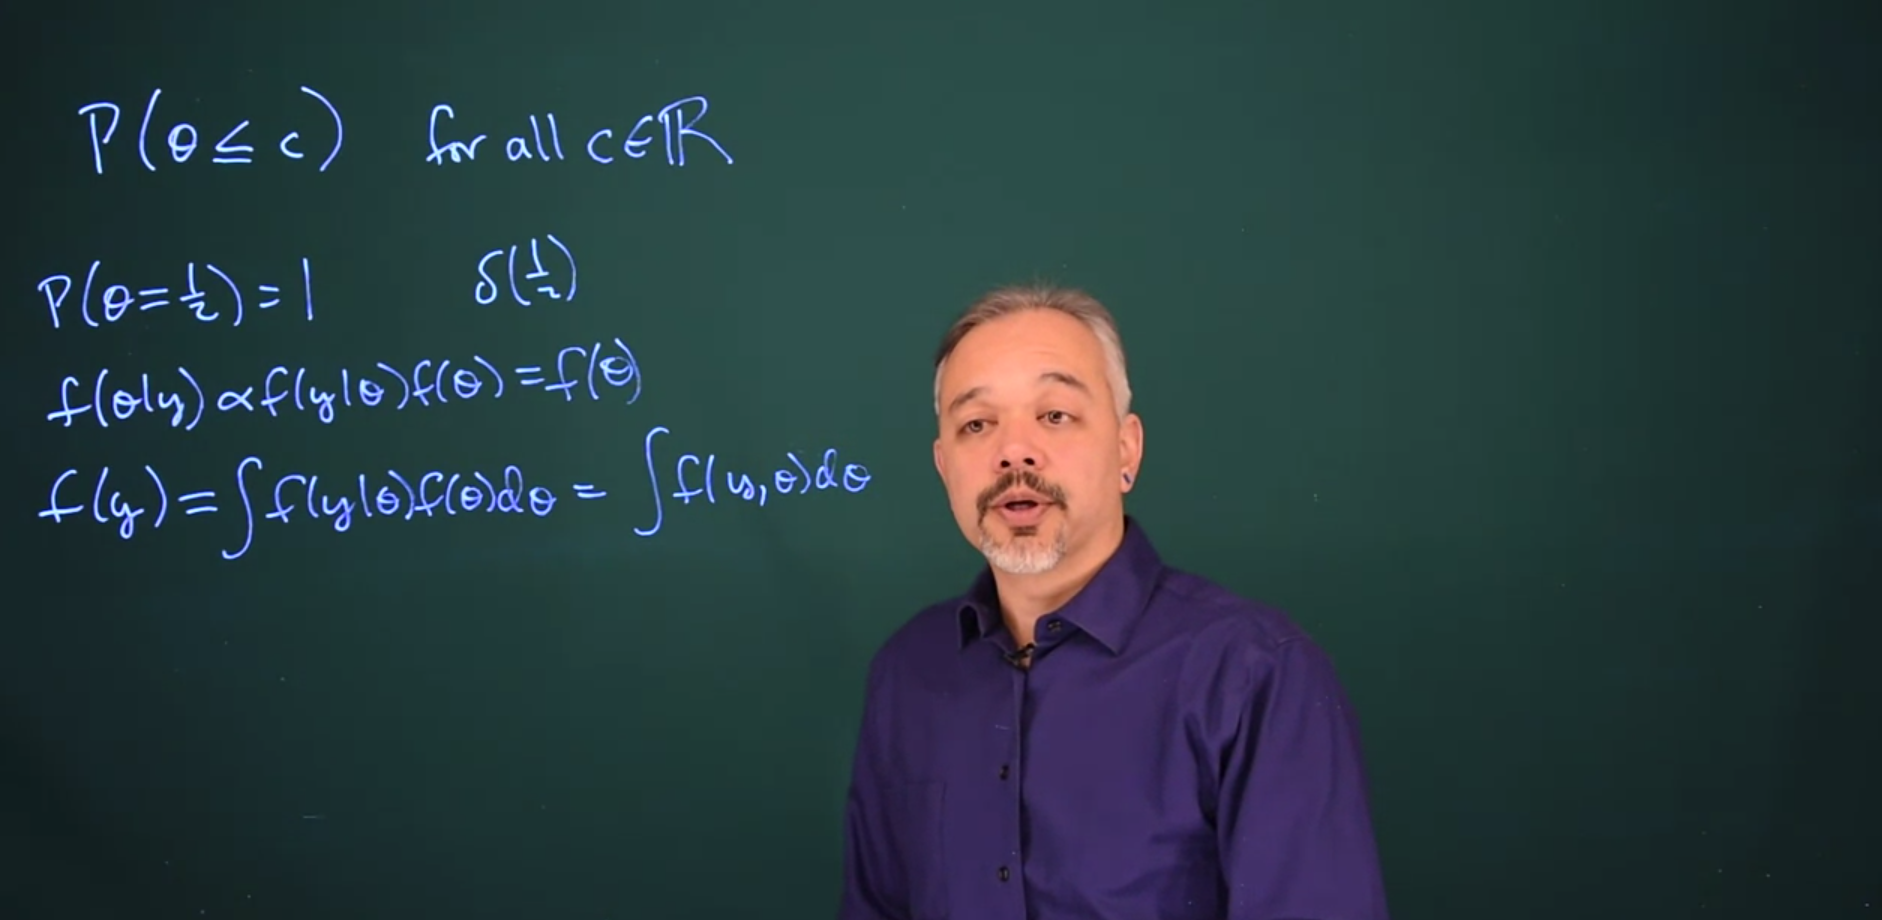
\includegraphics[width=53mm,height=\textheight,keepaspectratio]{images/c1l06-ss-01-prior-predictive-dist.png}

}

\caption{\label{fig-prior-predictive-distribution}Prior Predictive
Distribution}

\end{marginfigure}%

We can compute a predictive interval. This is an interval such that 95\%
of new observations are expected to fall into it. It's an interval for
the \textbf{data} rather than an interval for \(\theta\)

\begin{definition}[Prior Predictive
Distribution]\protect\hypertarget{def-prior-predictive-distribution}{}\label{def-prior-predictive-distribution}

The \textbf{prior predictive} distribution expresses our uncertainty
about a parameter, i.e.~the distribution of its possible values
\textbf{before} we observe any data.

\begin{equation}\phantomsection\label{eq-prior-predictive-definition}{
\begin{aligned}
f(y) &= \int{f(y \mid\theta)f(\theta)d\theta} &&\text {by Bayes theorem} 
\\&= \int{f(y, \theta)d\theta} && \text{the joint probability}
\end{aligned}
}\end{equation}

\begin{itemize}
\tightlist
\item
  \(f(y,\theta)\) is the \emph{joint density} of \(y\) and \(\theta\).
\item
  If we are integrating out \(\theta\), we will end up with a
  marginalized probability distribution of the data.
\item
  However, we may well decide to not integrate out \(\theta\)
  completely, so we will end up with a predictive interval.
\item
  But no data \(y\) has been observed, so this is the prior predictive
  before any data is observed.
\item
  It is used in \textbf{prior predictive checks} to assess whether the
  choice of prior distribution captures our prior beliefs.
\end{itemize}

\end{definition}

\section{Prior Predictive: Binomial
Example}\label{sec-prior-predictive-binomial-example}

\begin{marginfigure}

\centering{

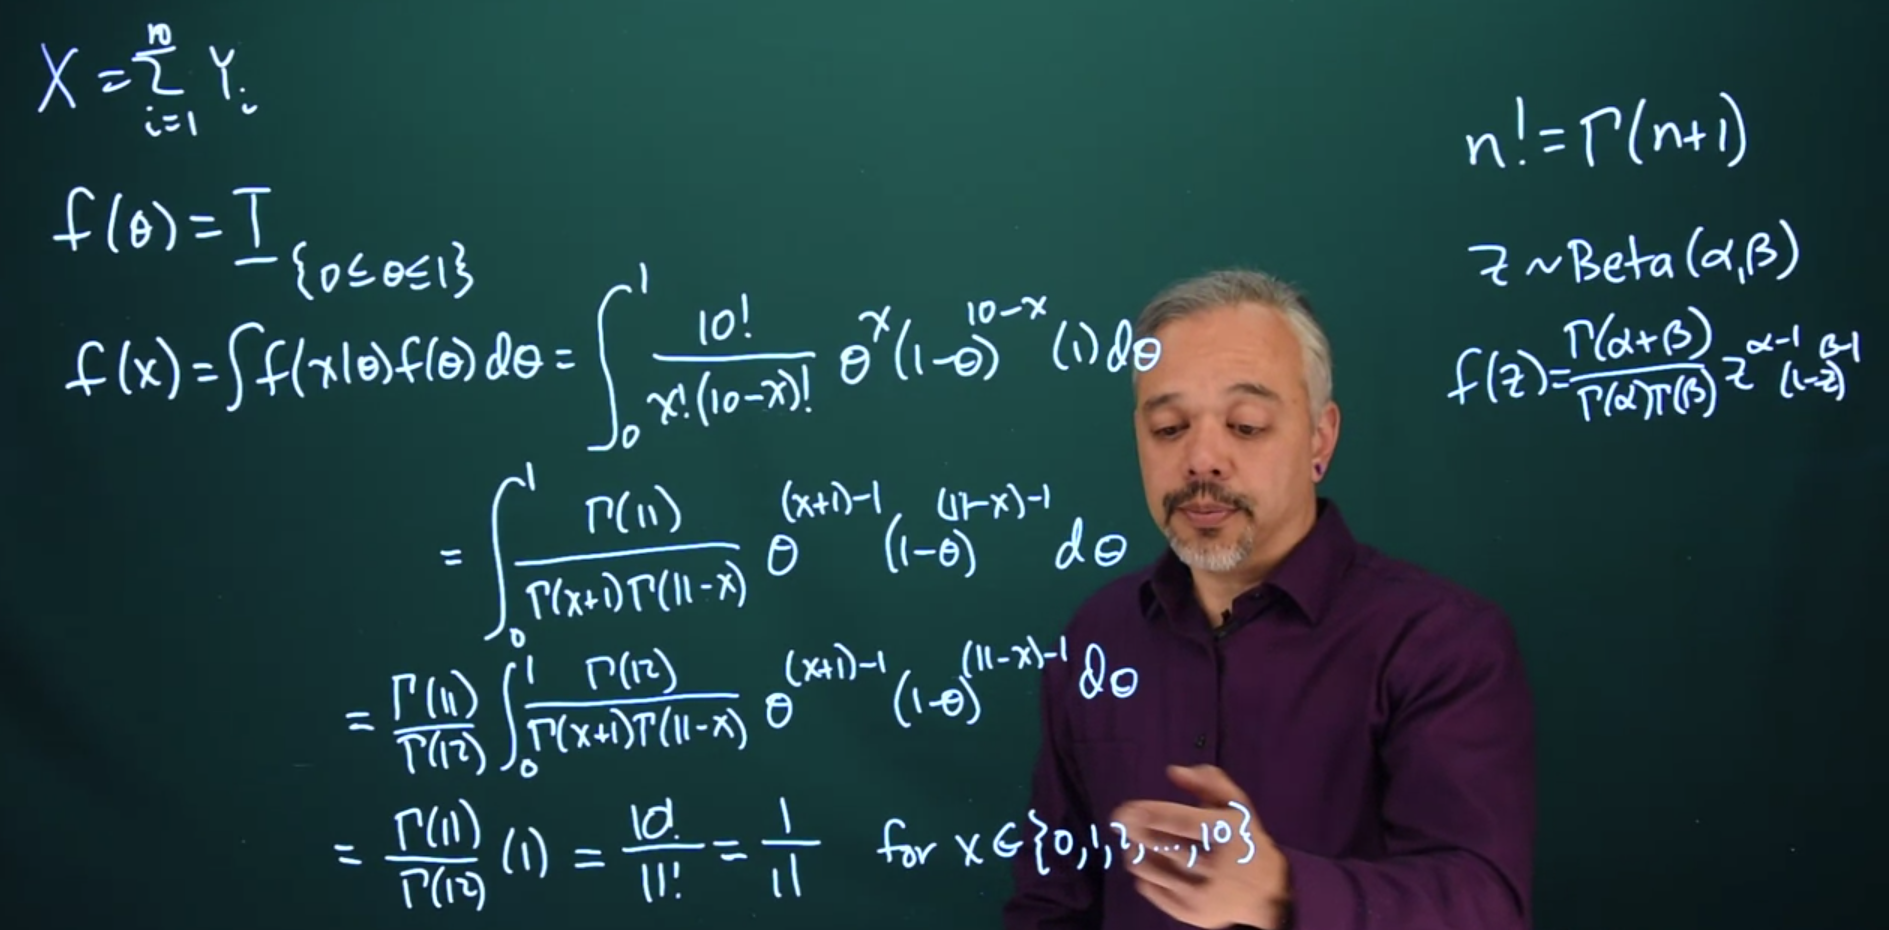
\includegraphics[width=53mm,height=\textheight,keepaspectratio]{images/c1l06-ss-02-prior-predictive-binomial-ex.png}

}

\caption{\label{fig-prior-predictive-binomial-example}Prior Predictive
Distribution Binomial Example}

\end{marginfigure}%

Suppose we're going to flip a coin 10 times and count the number of
heads we see. But we are thinking about this in advance of actually
doing it, and we are interested in the predictive distribution

\marginnote{\begin{footnotesize}

\textbf{Q. How many heads do we predict we're going to see?}

\textbf{Q. What's the probability that it shows up heads?}

\end{footnotesize}}

So, we'll need to choose a prior.

\[
N=10 \qquad \text {number of coin flips}
\]

Where \(Y_i\) represents individual coin flips. with Head being a
success

\[
Y \sim \text{Bernoulli}(\theta)
\]

Our data is the count of successes (heads) in N flips.

\[
X = \sum_{i=0}^N Y_i \qquad
\]

If we think that all possible coins or all possible probabilities are
equally likely, then we can put a prior for \(\theta\) that's flat over
the interval from 0 to 1. That is the Uniform prior
(Equation~\ref{eq-l3-uniform-pdf}):

\[
f(\theta)=\mathbb{I}_{[0 \le \theta \le 1]}
\]

The predictive probability is a \emph{binomial likelihood} times the
\emph{prior} = 1

\[
f(x) = \int f(x \mid\theta) f(\theta) d\theta = \int_0^1 \frac{10!}{x!(10-x)!} \theta^x(1-\theta)^{10-x}(1) d \theta
\]

Note that because we're interested in \(X\) at the end, it's important
that we distinguish between a Binomial density and a Bernoulli density.
Here we just care about the total count rather than the exact ordering
which would be Bernoulli.

For most of the analyses, we're doing, where we're interested in
\(\theta\) rather than x, the binomial and the Bernoulli are
interchangeable because the part in here that depends on \(\theta\) is
the same.

To solve this integral let us recall that:

\begin{equation}\phantomsection\label{eq-gamma-factorial}{
n! =\Gamma(n+1)
}\end{equation}

and

\[
Z \sim \text{Beta}(\alpha,\beta)
\]

The PDF for the beta distribution is given as:

\[
f(z)= \frac{\Gamma(\alpha+\beta)}{\Gamma(\alpha)\Gamma(\beta)} z^{\alpha−1}(1−z)^{\beta−1}I_{(0 < z <1)}
\]

where \(\alpha>0\) and \(\beta>0\).

\[
\begin{aligned}
  f(x) &= \int f(x \mid\theta) f(\theta) d\theta && \text {prior predictive dfn}
\\ &= \int_0^1 \frac{10!}{x!(10-x)!} \theta^x(1-\theta)^{10-x}( \mathbb{I_{[0,1]}}) d \theta && \text {subst. Binomial, } \mathbb{I_{[0,1]}}
\\ &= \int_0^1 \frac{\Gamma(11)}{\Gamma(x+1)\Gamma(11-x)} \theta^{(x+1)-1}(1-\theta)^{(11-x)-1}(1) d \theta && \text {convert to Beta(x+1,11-x), } 
\\ &=\frac{\Gamma(11)}{\Gamma(12)} 
\cancel{
  \int_0^1 \frac{\Gamma(12)}{\Gamma(x+1)\Gamma(11-x)}\theta^{(x+1)-1}(1-\theta)^{(11-x)-1}(1)d \theta
} && \text {integrating PDF=1 }
\\ &=\frac{\Gamma(11)}{\Gamma(12)} \times 1
 = \frac{10!}{11!}
 =\frac{1}{11} && \forall x \in \{1,2,\dots,10\}
\end{aligned}
\]

Thus we see that if we start with a uniform prior, we then end up with a
discrete uniform predictive density for \(X\). If all possible
\(\theta\) probabilities are equally likely, then all possible sums
\(X\) outcomes are equally likely.

The integral above is a beta density, all integrals of valid beta
densities equal one.

\[
f(x) = \frac{\Gamma(11)}{\Gamma(12)} = \frac{10!}{11!} = \frac{1}{11}
\]

\section{Posterior Predictive
Distribution}\label{posterior-predictive-distribution}

\begin{figure}[H]

{\centering \pandocbounded{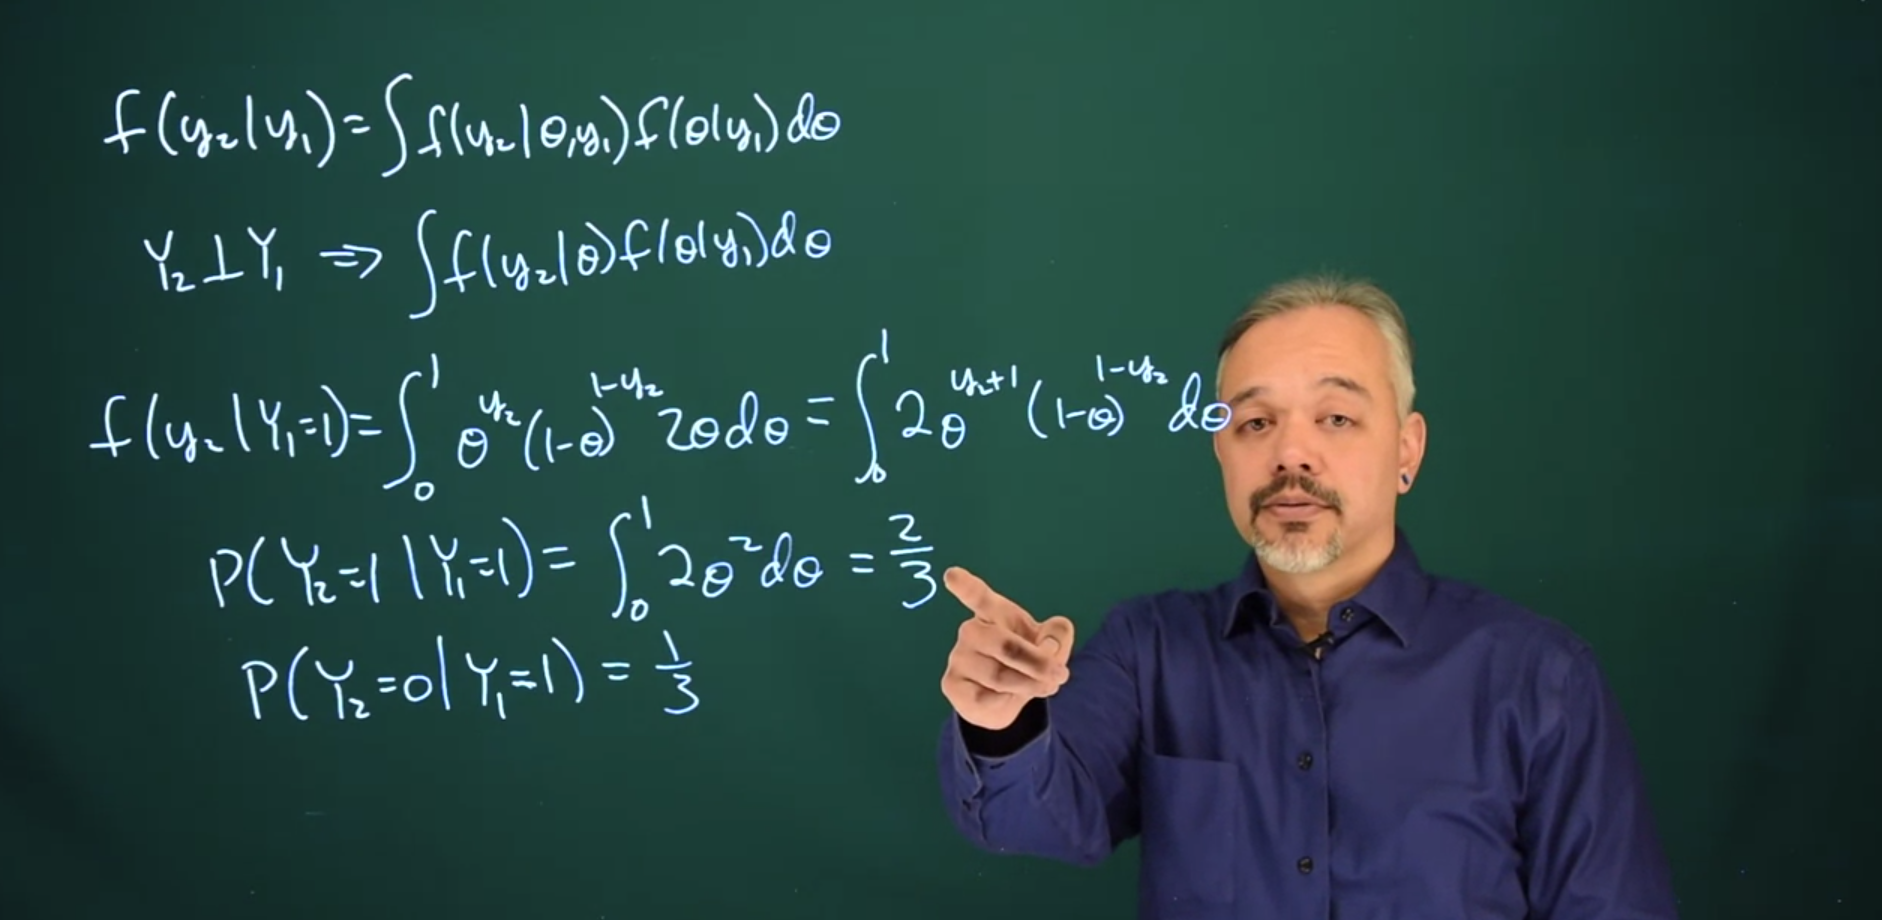
\includegraphics[keepaspectratio]{images/c1l06-ss-03-posterior-predicitive-distribution.png}}

}

\caption{Posterior Predictive Distribution}

\end{figure}%

What about after we've observed data? What's our posterior predictive
distribution?

Going from the previous example, let us observe after one flip that we
got a head.

We want to ask, \textbf{what's our predictive distribution for the
second flip, given we saw a head on the first flip?}

\section{Posterior Predictive
Distribution}\label{posterior-predictive-distribution-1}

The posterior predictive distribution is produced analogously to the
posterior predictive distribution by marginalizing the posterior with
respect to the parameter.

\begin{definition}[Posterior Predictive
Distribution]\protect\hypertarget{def-posterior-predictive-distribution}{}\label{def-posterior-predictive-distribution}

\begin{equation}\phantomsection\label{eq-posterior-predictive-distribution}{
\begin{aligned}
f(y_2 \mid y_1) &= \text{likelihood}\times \text{posterior} \\
&= \int{f(y_2 \mid \theta,y_1) \; f(\theta \mid y_1)}d\theta
\end{aligned}
}\end{equation}

\end{definition}

\begin{tcolorbox}[enhanced jigsaw, bottomrule=.15mm, colbacktitle=quarto-callout-tip-color!10!white, leftrule=.75mm, bottomtitle=1mm, titlerule=0mm, title=\textcolor{quarto-callout-tip-color}{\faLightbulb}\hspace{0.5em}{Marginalizing distribution}, rightrule=.15mm, toprule=.15mm, colback=white, left=2mm, toptitle=1mm, arc=.35mm, opacitybacktitle=0.6, coltitle=black, breakable, opacityback=0, colframe=quarto-callout-tip-color-frame]

Suppose we have an experiment with events based on two RVs: - (C) a coin
toss - (D) and a dice toss. And we call this event
\(X = \mathbb{P}r(C,D) = \mathbb{P}r(C) \times \mathbb{P}r(D)\)

\begin{longtable}[]{@{}llllllll@{}}
\toprule\noalign{}
C D & 1 & 2 & 3 & 4 & 5 & 6 & \(\mathbb{P}r(C)\) \\
\midrule\noalign{}
\endhead
\bottomrule\noalign{}
\endlastfoot
H & 1/12 & 1/12 & 1/12 & 1/12 & 1/12 & 1/12 & 6/12 \\
T & 1/12 & 1/12 & 1/12 & 1/12 & 1/12 & 1/12 & 6/12 \\
\(\mathbb{P}r(D)\) & 2/12 & 2/12 & 2/12 & 2/12 & 2/12 & 2/12 & 1 \\
\end{longtable}

We can recover the \(\mathbb{P}r(C)\) coin's distribution or the dice
distribution \(\mathbb{P}r(D)\) by marginalization. \(\mathbb{P}r(X)\)
This is done by summing over the row or columns.

The marginal distribution let us subset a joint distribution. The
marginal distribution has removed the uncertainty due to a parameter.

we use three terms interchangeably :

\begin{itemize}
\tightlist
\item
  marginalizing the posterior w.r.t. \(\theta\)
\item
  integrating/summing over \(\theta\)
\item
  integrating \(\theta\) out
\end{itemize}

The first is the real idea, the others are the techniques being used to
do it. For a predictive distribution we may want to marginalize all the
parameters so we end up with the RV we wish to predict.

\end{tcolorbox}

We're going to assume that \(Y_2\) is independent of \(Y_1\). Therefore,

\[
f(y_2 \mid y_1) = \int{f(y_2 \mid \theta)f(\theta \mid y_1)d\theta}
\]

Suppose we're thinking of a uniform distribution for \(\theta\) and we
observe the first flip is a ``head''. What do we predict for the second
flip?

This is no longer going to be a uniform distribution like it was before
because we have some data. We're going to think it's more likely that
we're going to get a second head. We think this because since we
observed a head \(\theta\) is now likely to be at least \(\frac{1}{2}\)
possibly larger.

\[
f(y_2 \mid Y_1 = 1) = \int_0^1{\theta^{y_2}(1-\theta)^{1-y_2}2\theta d\theta}
\]

\[
f(y_2 \mid Y_1 = 1) = \int_0^1{2\theta^{y_2 + 1}(1-\theta)^{1-y_2}d\theta}
\]

We could work this out in a more general form, but in this case, \(Y_2\)
has to take the value \(0\) or \(1\). The next flip is either going to
be heads or tails so it's easier to just plop in a particular example.

\[
\mathbb{P}r(Y_2 = 1 \mid Y_1 = 1) = \int_\theta^1 {2 \theta^2 d \theta} = \frac{2}{3}
\]

\[
\mathbb{P}r(Y_2 = 0 \mid Y_1 = 1) = 1 - \mathbb{P}r(Y_2 = 1 \mid Y_1 = 1) = 1 - \frac{2}{3} = \frac{1}{3}
\]

We can see here that the posterior is a combination of the information
in the prior and the information in the data. In this case, our prior is
like having two data points, one head and one tail.

Saying we have a \textbf{uniform prior} for \(\theta\) is equivalent in
an information sense to saying ``we have observed one `Head' and one
`Tail'\,''.

So then when we observe one head, it's like we now have seen two heads
and one tail. So our predictive distribution for the second flip says if
we have two heads and one tail, then we have a \(\frac{2}{3}\)
probability of getting another head and a \(\frac{1}{3}\) probability of
getting another tail.

\chapter{Homework Posterior Probabilities -
M3L6HW1}\label{homework-posterior-probabilities---m3l6hw1}

Bayesian Statistics: From Concept to Data Analysis

\hfill\break

\begin{tcolorbox}[enhanced jigsaw, bottomrule=.15mm, colbacktitle=quarto-callout-caution-color!10!white, leftrule=.75mm, bottomtitle=1mm, titlerule=0mm, title=\textcolor{quarto-callout-caution-color}{\faFire}\hspace{0.5em}{Caution}, rightrule=.15mm, toprule=.15mm, colback=white, left=2mm, toptitle=1mm, arc=.35mm, opacitybacktitle=0.6, coltitle=black, breakable, opacityback=0, colframe=quarto-callout-caution-color-frame]

Section omitted to comply with the Honor Code

\end{tcolorbox}

\chapter{M3L7 - Binomial Data}\label{m3l7---binomial-data}

Bayesian Statistics: From Concept to Data Analysis

\hfill\break

\section{Bernoulli/Binomial likelihood with a uniform
prior}\label{bernoullibinomial-likelihood-with-a-uniform-prior}

\begin{marginfigure}

\centering{

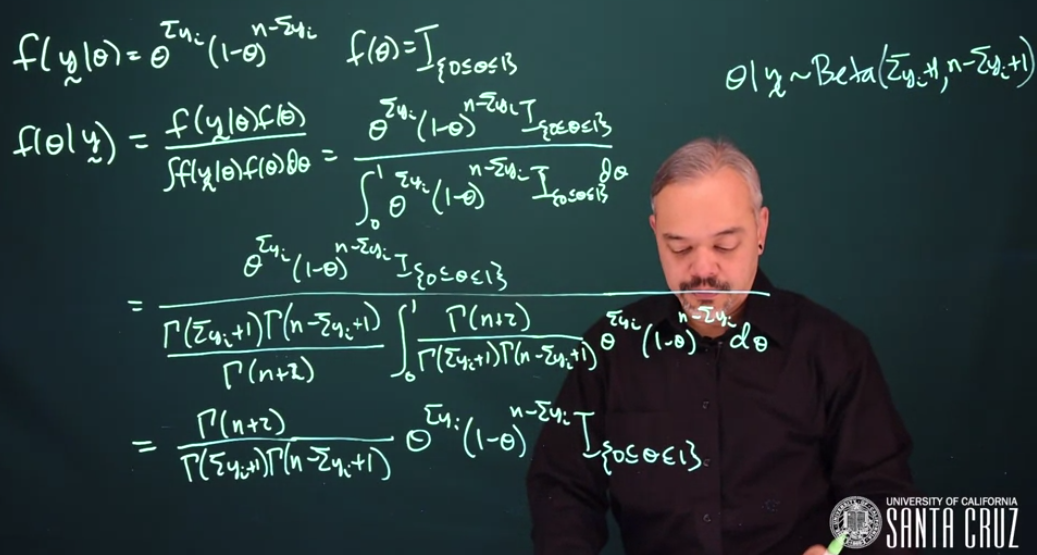
\includegraphics[width=53mm,height=\textheight,keepaspectratio]{images/c1l07-ss-01-binomial-likelihood-uniform-prior.png}

}

\caption{\label{fig-binomial-likelihood-uniform-prior}Binomial
likelihood with a Uniform prior}

\end{marginfigure}%

When we use a uniform prior for a Bernoulli likelihood, we get a beta
posterior.

The Bernoulli likelihood of \(\vec Y \mid \theta\) is

\[
{\color{green}f(\vec Y \mid \theta) = {\theta^{\sum{y_i}}(1-\theta)^{n - \sum{y_i}}}} \qquad \text{Bernoulli Likelihood}
\]

Our prior for \(\theta\) is just a Uniform distribution

\[
{\color{red}f(\theta) = I_{\{0 \le \theta \le 1\}} }\qquad \text {Uniform prior}
\]

Thus our posterior for \(\theta\) is \[
\begin{aligned}
f(\theta \mid y) & = \frac{f(y \mid \theta) f(\theta)}{\int f(y \mid \theta)f(\theta) \, d\theta} & \text{Bayes law} \\
& = \frac{\theta^{\sum{y_i}} (1 - \theta)^{n - \sum{y_i}} \mathbb{I}_{\{0 \le \theta \le 1\}}}{\int_0^1 \theta^{\sum{y_i}}(1 - \theta)^{n - \sum{y_i}} \mathbb{I}_{\{0 \le \theta \le 1\}} \, d\theta} & \text{subst. Likelihood \& Prior} \\
& = \frac{\theta^{\sum{y_i}} (1-\theta)^{n - \sum{y_i}} \mathbb{I}_{\{0 \le \theta \le 1\}}}{\frac{\Gamma(\sum{y_i} + 1)\Gamma(n - \sum{y_i} + 1)}{\Gamma(n + 2)} \cancel{\int_0^1 \frac{\Gamma(n + 2)}{\Gamma(\sum{y_i} + 1) \Gamma(n - \sum{y_i} + 1)} \theta^{\sum{y_i}} (1 - \theta)^{n - \sum{y_i}} \, d\theta}} & \text{Beta PDF integrates to 1} \\
& = \frac{\Gamma(n + 2)}{\Gamma(\sum{y_i}+ 1) \Gamma(n - \sum{y_i}+ 1)} \theta^{\sum{y_i}}(1 - \theta)^{n - \sum{y_i}} \mathbb{I}_{\{0 \le \theta \le 1\}} & \text{simplifying} \\
& = \mathrm{Beta} \left (\sum{y_i} + 1, n - \sum{y_i} + 1 \right )
\end{aligned}
\]

Where we used a trick of recognizing the denominator as a \emph{Beta
distribution} (Equation~\ref{eq-beta-pdf}) we then manipulate it to take
the exact form of \emph{Beta}. We can then cancel it since the
\emph{Beta density} integrates to \(1\), we can simplify this as From
here we can see that the posterior follows a \emph{Beta distribution}

\[
\theta \mid y \sim \mathrm{Beta}\left (\sum{y_i} + 1, n - \sum{y_i} + 1 \right )
\]

\index{Fisher, R.A.} \index{{Fisher, Ronald Aylmer}|see{Fisher, R.A.}}
\index{{Fisher, Ronald}|see{Fisher, R.A.}} \index{Jeffreys, Harold}

\begin{marginfigure}

\centering{

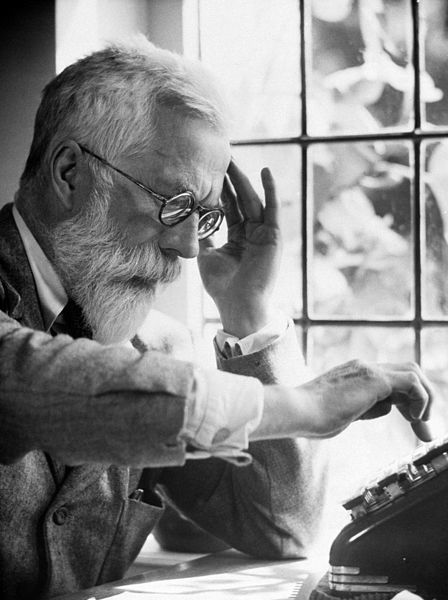
\includegraphics[width=53mm,height=\textheight,keepaspectratio]{images/bio-rafisher.jpg}

}

\caption{\label{fig-rafisher}R.A. Fisher}

\end{marginfigure}%

\begin{tcolorbox}[enhanced jigsaw, bottomrule=.15mm, colbacktitle=quarto-callout-tip-color!10!white, leftrule=.75mm, bottomtitle=1mm, titlerule=0mm, title=\textcolor{quarto-callout-tip-color}{\faLightbulb}\hspace{0.5em}{Historical Note on Sir Ronald Aylmer Fisher FRS}, rightrule=.15mm, toprule=.15mm, colback=white, left=2mm, toptitle=1mm, arc=.35mm, opacitybacktitle=0.6, coltitle=black, breakable, opacityback=0, colframe=quarto-callout-tip-color-frame]

R.A. Fisher's objection to the Bayesian approach is that ``The theory of
inverse probability \textbf{is founded upon an error, and must be wholly
rejected''} (Fisher 1925) was specifically referring to this example of
a''Binomial with a Uniform prior''. The gist of it is that the posterior
depends on the parametrization of the prior.(Aldrich 2008). Sir Harold
Jeffreys FRS who corresponded with Fisher went on to develop his
eponymous priors which were invariant to reparametrization. Which we
will consider in Section~\ref{sec-jeffreys-prior}

\end{tcolorbox}

\section{Conjugate Priors}\label{sec-conjugate-beta-priors}

\begin{marginfigure}

\centering{

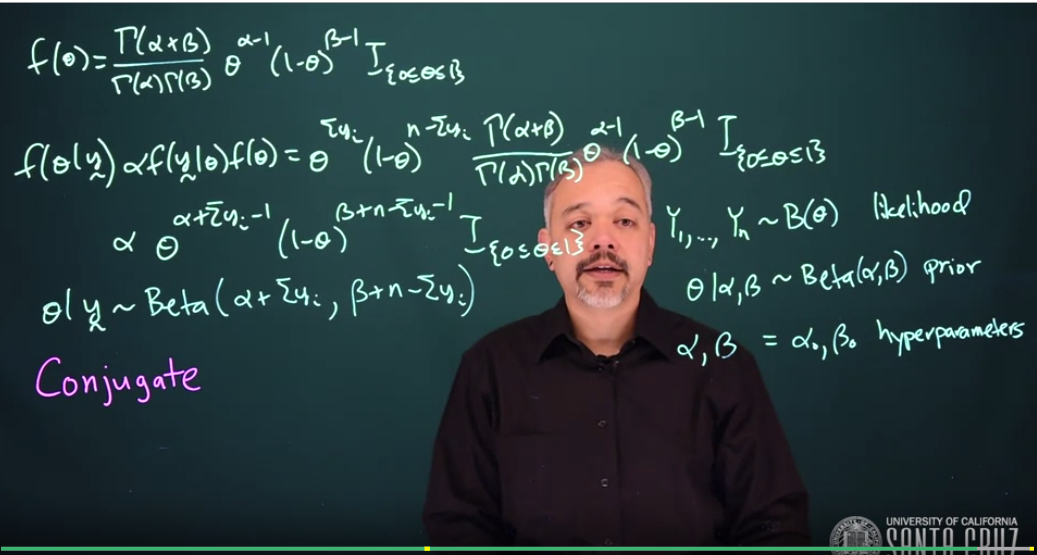
\includegraphics[width=53mm,height=\textheight,keepaspectratio]{images/c1l07-ss-03-conjugate-priors.png}

}

\caption{\label{fig-s03-conjugate-priors}Conjugate Priors}

\end{marginfigure}%

The Uniform distribution is \(\mathrm{Beta}(1, 1)\)

Any beta distribution is conjugate for the \emph{Bernoulli
distribution}. Any \emph{beta prior} will give a \emph{beta posterior}.

\[
f(\theta) = \frac{\Gamma(\alpha + \beta)}{\Gamma(\alpha)\Gamma(\beta)}\theta^{\alpha - 1}(1-\theta)^{\beta -1}\mathbb{I}_{\{\theta \le \theta \le 1\}}
\]

\[
f(\theta \mid y) \propto f(y \mid \theta)f(\theta) = \theta^{\sum{y_i}}(1-\theta)^{n - \sum{y_i}}\frac{\Gamma(\alpha + \beta)}{\Gamma(\alpha)\Gamma(\beta)}\theta^{\alpha - 1}(1 - \theta)^{\beta - 1}\mathbb{I}_{\{\theta \le \theta \le 1\}}
\]

\[
f(y \mid\theta)f(\theta) \propto \theta^{\alpha + \sum{y_i}-1}(1-\theta)^{\beta + n - \sum{y_i} - 1}
\]

Thus we see that this is a beta distribution

\[
\theta \mid y \sim \mathrm{Beta}(\alpha + \sum{y_i}, \beta + n - \sum{y_i})
\]

When \(\alpha\) and \(\beta\) are one like in the uniform distribution,
then we get the same result as earlier.

This whole process where we choose a particular form of prior that works
with a likelihood is called using a conjugate family.

A family of distributions is referred to as conjugate if when you use a
member of that family as a prior, you get another member of that family
as your posterior.

The beta distribution is conjugate for the Bernoulli distribution. It's
also conjugate for the binomial distribution. The only difference in the
binomial likelihood is that there is a combinatorics term. Since that
does not depend on \(\theta\), we get the same posterior.

\index{prior!conjugate} We often use conjugate priors because they make
life much simpler, sticking to conjugate families allows us to get
closed-form solutions easily.

If the family is flexible enough, then you can find a member of that
family that closely represents your beliefs.

\begin{itemize}
\tightlist
\item
  the Uniform distribution can be written as the \(\mathrm{Beta}(1,1)\)
  prior.
\item
  Any \emph{Beta prior} will result in a \emph{Beta posterior}.
\item
  \emph{Beta} is conjugate for Binomial and for Bernoulli
\end{itemize}

\section{Posterior mean and effective sample
size}\label{sec-effective-sample-size}

\begin{marginfigure}

\centering{

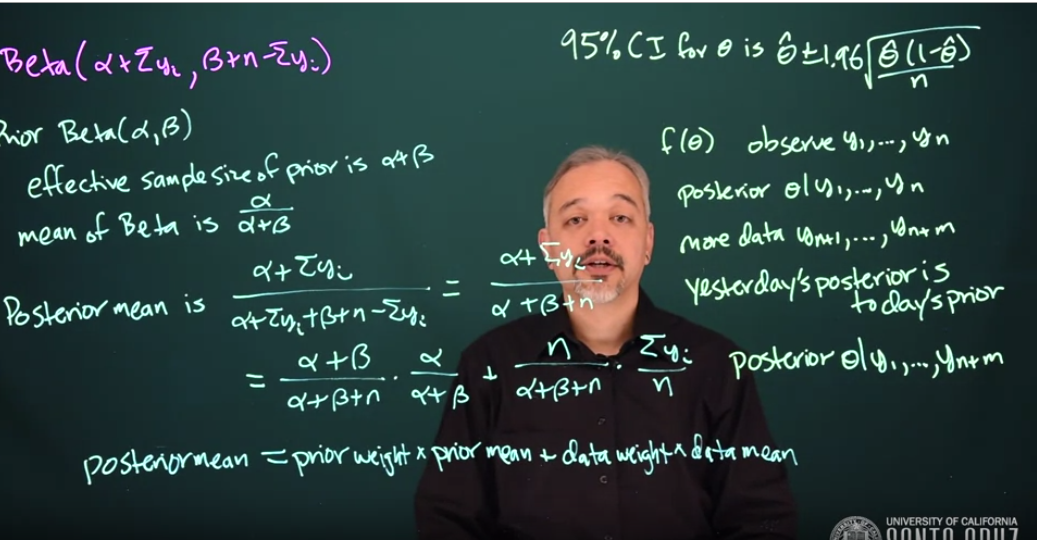
\includegraphics[width=53mm,height=\textheight,keepaspectratio]{images/c1l07-ss-04-effective-sample-size.png}

}

\caption{\label{fig-s04-effective-sample-size}Effective Sample Size}

\end{marginfigure}%

Returning to the \emph{Beta} posterior model it is clear how both the
prior and the data contribute to the posterior.

For a prior \(\mathrm{Beta}(\alpha,\beta)\) we can say that the
\textbf{effective sample size} of the prior is

\begin{equation}\phantomsection\label{eq-beta-ess}{
\alpha + \beta \qquad \text {(ESS)}
}\end{equation}

Recall that the expected value or mean of a \emph{Beta} distribution is
\(\frac{\alpha}{\alpha + \beta}\)

Therefore we can derive the posterior mean as

\begin{equation}\phantomsection\label{eq-beta-posterior-mean-derivation}{
\begin{aligned}
   posterior_{mean} &= \frac{\alpha + \sum{y_i}}{\alpha + \sum{y_i}+\beta + n - \sum{y_i}}
\\                  &= \frac{\alpha+\sum{y_i}}{\alpha + \beta + n}
\\                  &= \frac{\alpha + \beta}{\alpha + \beta + n}\frac{\alpha}{\alpha + \beta} + \frac{n}{\alpha + \beta + n}\frac{\sum{y_i}}{n}
\\ &= (\text{prior weight} \times \text{prior mean}) + (\text{data weight} \times \text{data mean})
\end{aligned}
}\end{equation}

i.e.~The \textbf{posterior mean} is a weighted average of the
\textbf{prior mean} and the \textbf{data mean}.

\index{MCMC!effective sample size} This effective sample size gives you
an idea of how much data you would need to make sure that your prior
does not have much influence on your posterior.

If \(\alpha + \beta\) is small compared to \(n\) then the posterior will
largely just be driven by the data. If \(\alpha + \beta\) is large
relative to \(n\) then the posterior will be largely driven by the
prior.

We can make a 95\% credible interval using our posterior distribution
for \(\theta\) . We can find an interval that has \(95 \%\) probability
of containing \(\theta\).

\index{sequential analysis} Using Bayesian Statistics we can do
\emph{sequential analysis} by doing a sequential update every time we
get new data. We can get a new posterior, and we just use our previous
Posterior as a Prior for doing another update using Bayes' theorem.

\begin{marginfigure}

\centering{

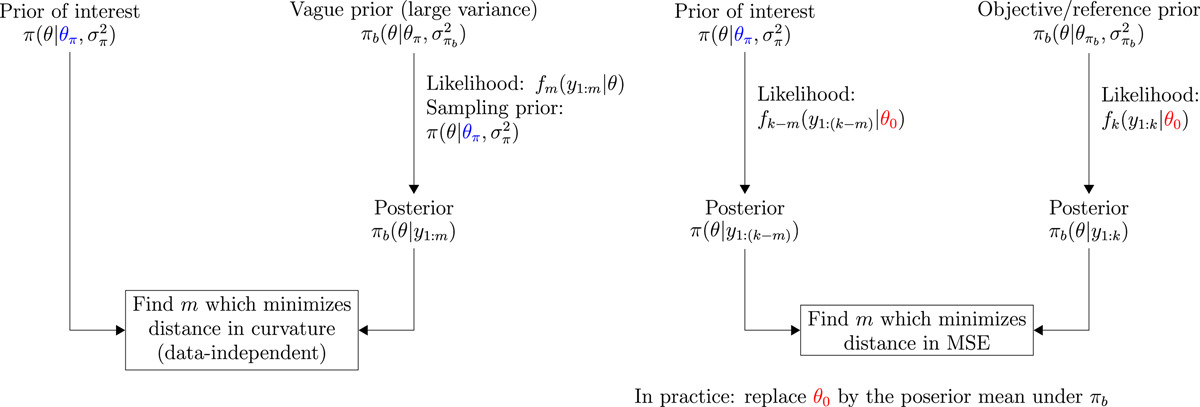
\includegraphics[width=53mm,height=\textheight,keepaspectratio]{images/c1l07-ss-03-ess-paper.jpg}

}

\caption{\label{fig-ess-paper}ESS algorithms}

\end{marginfigure}%

\begin{itemize}
\tightlist
\item
  for a \emph{Beta prior}, its \emph{effective sample size} is \(a + b\)
\item
  if \(n >> \alpha+\beta\) the posterior will be predominantly
  determined by the prior
\item
  if \(n << \alpha+\beta\) the posterior will be predominantly
  determined by the data
\item
  the idea of an effective sample size of the prior is a useful concept
  to work with.
\item
  (Wiesenfarth and Calderazzo 2020)

  \begin{itemize}
  \item
    Effective Sample Size (ESS)
  \item
    Effective Current Sample size (ECSS)
  \item
    with (Morita, Thall, and Müller 2008) on the left and ECSS on the
    right
  \end{itemize}
\end{itemize}

\begin{marginfigure}

\centering{

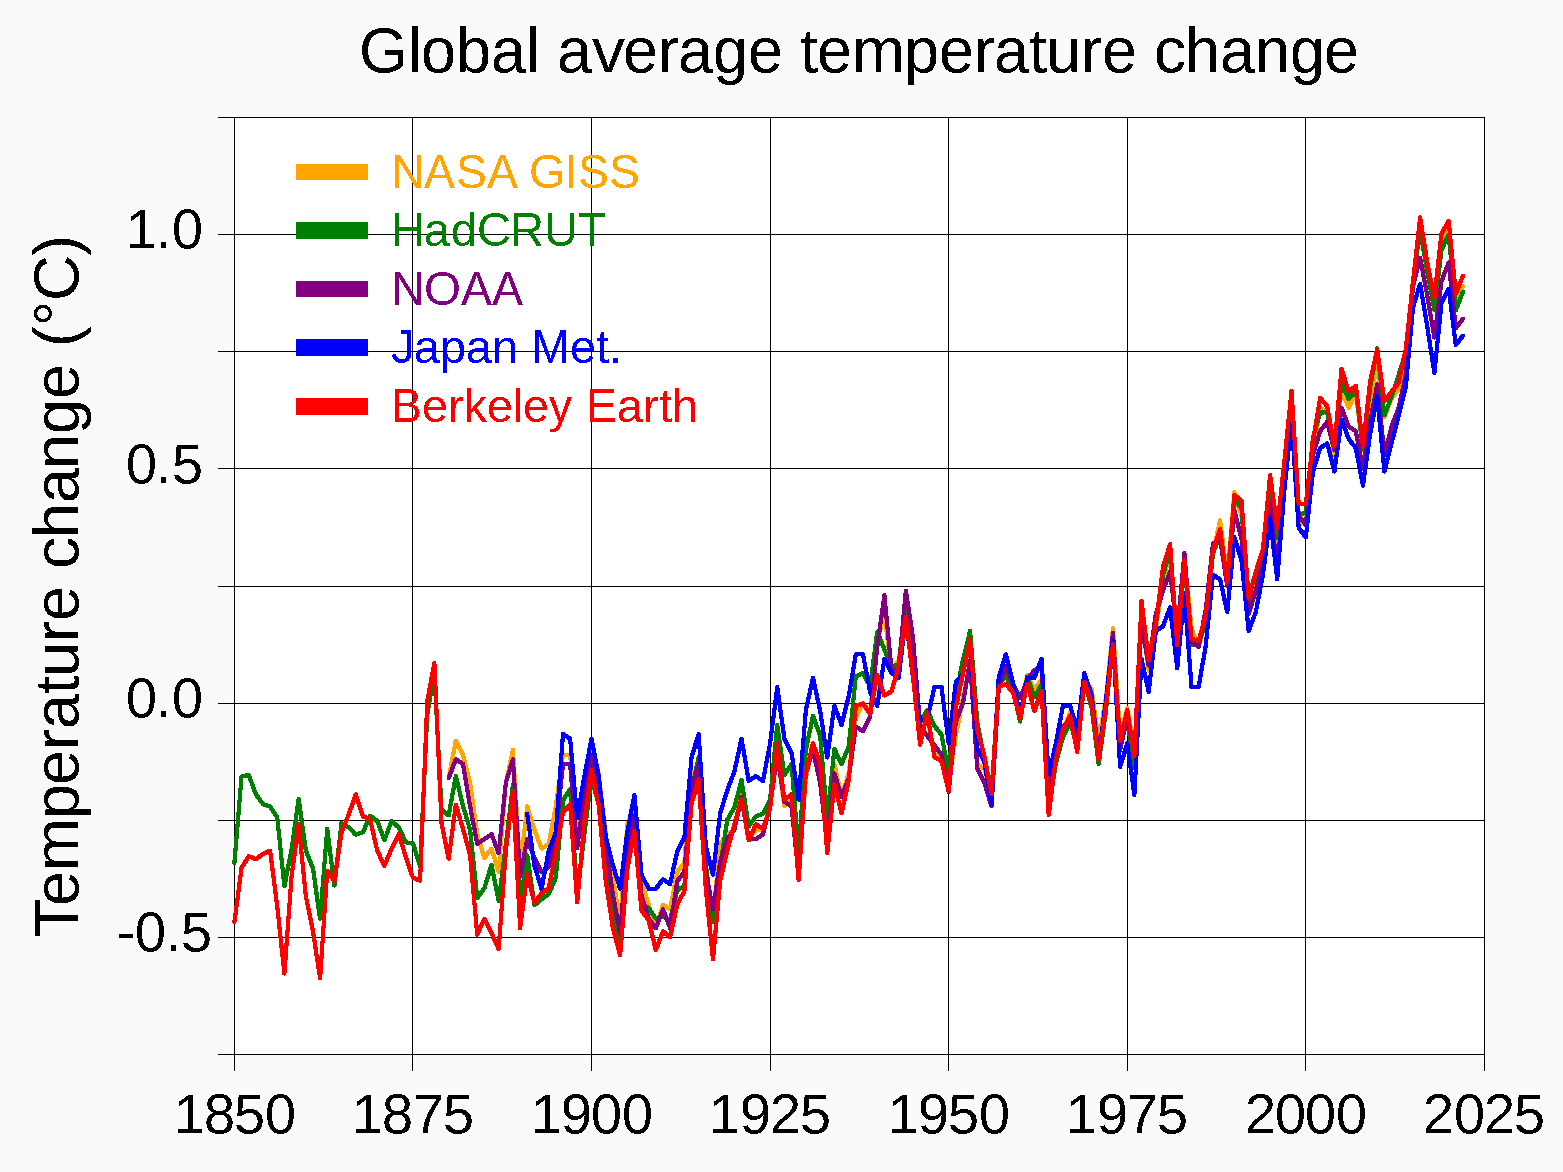
\includegraphics[width=53mm,height=\textheight,keepaspectratio]{index_files/mediabag/images/20200324_Global_average_temperature_-_NASA-GISS_HadCrut_NOAA_Japan_BerkeleyE.pdf}

}

\caption{\label{fig-200-year-meterological}200 year meteorological
record}

\end{marginfigure}%

\begin{marginfigure}

\centering{

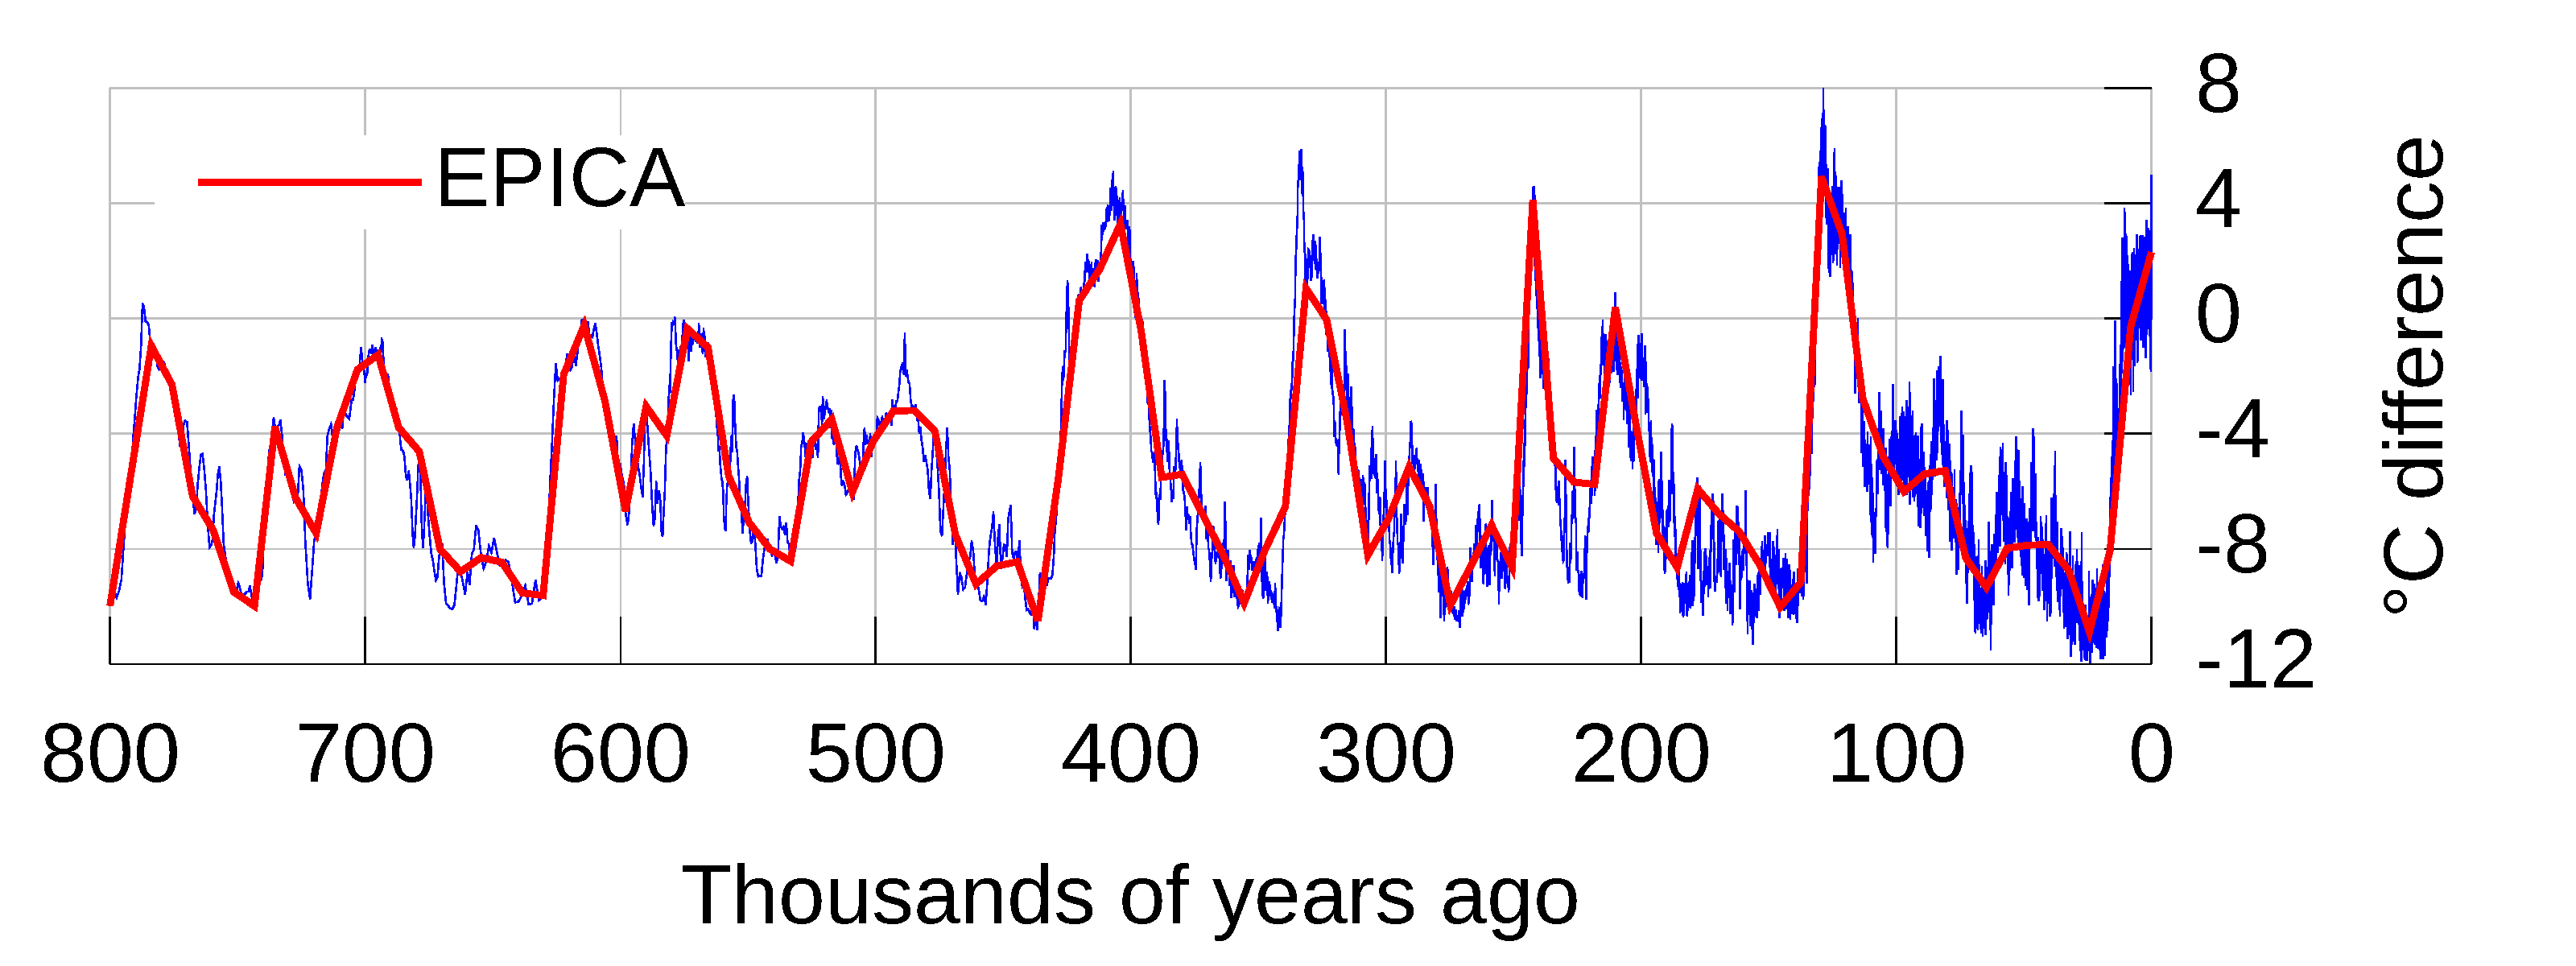
\includegraphics[width=53mm,height=\textheight,keepaspectratio]{index_files/mediabag/images/EPICA_temperature_plot.pdf}

}

\caption{\label{fig-800K-year-ice-core}800K year ice core record}

\end{marginfigure}%

\begin{marginfigure}

\centering{

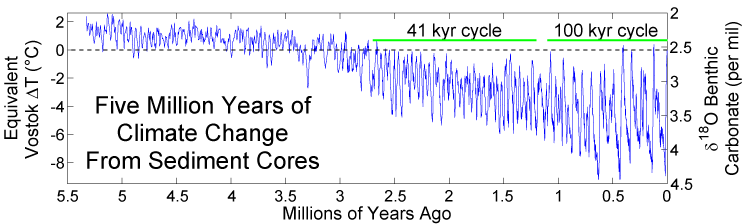
\includegraphics[width=53mm,height=\textheight,keepaspectratio]{images/Five_Myr_Climate_Change.png}

}

\caption{\label{fig-five-year-deep-sea}5M year deep sea record}

\end{marginfigure}%

\begin{exercise}[Discussion on Prior
elicitation]\protect\hypertarget{exr-prior-elicitation}{}\label{exr-prior-elicitation}

~

\begin{quote}
Suppose we are interested in global temperatures, and that we have a
summary measure that represents the average global temperature for each
year. Now we could ask ``What is the probability that next year will
have a higher average global temperature than this year?'' What would be
your choice of prior and why? Be specific about the distribution and its
parameters. You may use any other information that you want to bring
into this problem.
\end{quote}

\end{exercise}

\begin{tcolorbox}[enhanced jigsaw, bottomrule=.15mm, colbacktitle=quarto-callout-tip-color!10!white, leftrule=.75mm, bottomtitle=1mm, titlerule=0mm, title=\textcolor{quarto-callout-tip-color}{\faLightbulb}\hspace{0.5em}{Response}, rightrule=.15mm, toprule=.15mm, colback=white, left=2mm, toptitle=1mm, arc=.35mm, opacitybacktitle=0.6, coltitle=black, breakable, opacityback=0, colframe=quarto-callout-tip-color-frame]

It is possible to get historical estimates using:

\begin{itemize}
\item
  Meteorological and satellites for the last 200 years.
  Figure~\ref{fig-200-year-meterological}
\item
  Ice cores for the last 800,000 years
  Figure~\ref{fig-800K-year-ice-core}
\item
  Deep sea sediment oxygen 18 isotope fractation for the last 5 million
  years. Figure~\ref{fig-five-year-deep-sea}
\end{itemize}

or yearly temperature data from 1850 till today based on meteorological
readings. We can also consider Greenland ice core data covering 800,000
years.

One simple way is to model the yearly temperature as a random walk

i.e.~Each year is a Bernoulli trial where success is the temperature
getting warmer. We can then use the historical data since 1800 to
estimate theta the probability that we get warmer.

I suppose we can use a Binomial prior with parameters for alpha the
count of years the temperature increased and N for the total number of
years and p the probability the a given year is hotter than the
previous.

\end{tcolorbox}

\section{Data Analysis Example in R}\label{data-analysis-example-in-r}

Suppose we're giving two students a multiple-choice exam with 40
questions, where each question has four choices. We don't know how much
the students have studied for this exam, but we think that they'll do
better than just guessing randomly

\begin{enumerate}
\def\labelenumi{\arabic{enumi}.}
\tightlist
\item
  What are the parameters of interest?
\end{enumerate}

The parameters of interests are \(\theta_1 = true\) the probability that
the first student will answer a question correctly, \(\theta_2 = true\)
the probability that the second student will answer a question
correctly.

\begin{enumerate}
\def\labelenumi{\arabic{enumi}.}
\setcounter{enumi}{1}
\tightlist
\item
  What is our likelihood?
\end{enumerate}

The likelihood is \(\mathrm{Binomial}(40, \theta)\) if we assume that
each question is independent and that the probability a student gets
each question right is the same for all questions for that student.

\begin{enumerate}
\def\labelenumi{\arabic{enumi}.}
\setcounter{enumi}{2}
\tightlist
\item
  What prior should we use?
\end{enumerate}

The \textbf{Conjugate Prior} is a \textbf{Beta Distribution}. We can
plot the density with \texttt{dbeta}

\begin{Shaded}
\begin{Highlighting}[]
\NormalTok{theta }\OtherTok{=} \FunctionTok{seq}\NormalTok{(}\AttributeTok{from =} \DecValTok{0}\NormalTok{, }\AttributeTok{to =} \DecValTok{1}\NormalTok{, }\AttributeTok{by =} \FloatTok{0.1}\NormalTok{)}
\CommentTok{\# Uniform}
\FunctionTok{plot}\NormalTok{(theta, }\FunctionTok{dbeta}\NormalTok{(theta, }\DecValTok{1}\NormalTok{, }\DecValTok{1}\NormalTok{), }\AttributeTok{type =} \StringTok{\textquotesingle{}l\textquotesingle{}}\NormalTok{)}
\end{Highlighting}
\end{Shaded}

\pandocbounded{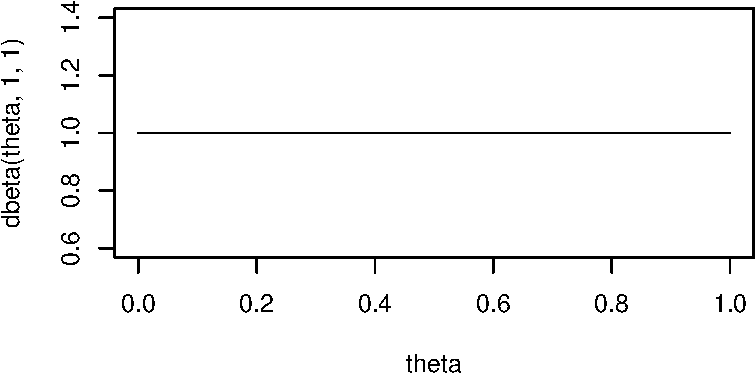
\includegraphics[keepaspectratio]{C1-L07_files/figure-pdf/C1-L07-1-1.pdf}}

\begin{Shaded}
\begin{Highlighting}[]
\CommentTok{\# Prior mean 2/3}
\FunctionTok{plot}\NormalTok{(theta, }\FunctionTok{dbeta}\NormalTok{(theta, }\DecValTok{4}\NormalTok{, }\DecValTok{2}\NormalTok{), }\AttributeTok{type =} \StringTok{\textquotesingle{}l\textquotesingle{}}\NormalTok{)}
\end{Highlighting}
\end{Shaded}

\pandocbounded{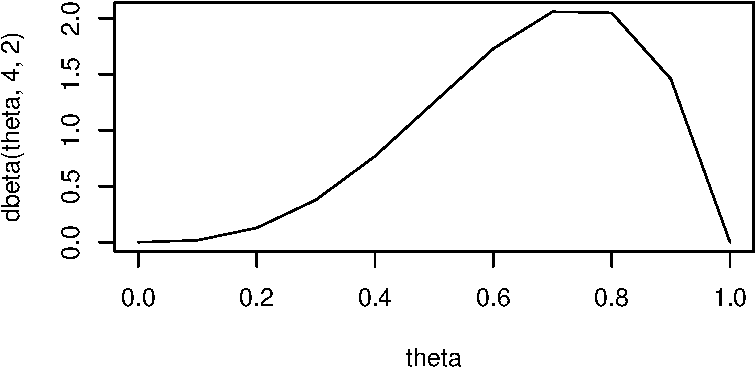
\includegraphics[keepaspectratio]{C1-L07_files/figure-pdf/C1-L07-1-2.pdf}}

\begin{Shaded}
\begin{Highlighting}[]
\CommentTok{\# Prior mean 2/3 but higher effect size (more concentrated at mean)}
\FunctionTok{plot}\NormalTok{(theta, }\FunctionTok{dbeta}\NormalTok{(theta, }\DecValTok{8}\NormalTok{, }\DecValTok{4}\NormalTok{), }\AttributeTok{type =} \StringTok{\textquotesingle{}l\textquotesingle{}}\NormalTok{)}
\end{Highlighting}
\end{Shaded}

\pandocbounded{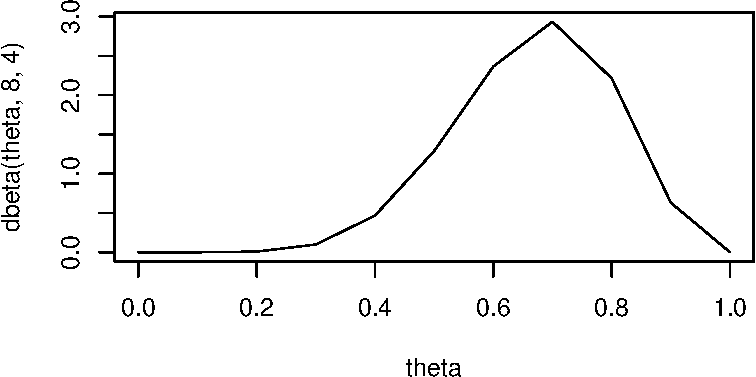
\includegraphics[keepaspectratio]{C1-L07_files/figure-pdf/C1-L07-1-3.pdf}}

\begin{enumerate}
\def\labelenumi{\arabic{enumi}.}
\setcounter{enumi}{3}
\tightlist
\item
  What are the prior probabilities \(\mathbb{P}r(\theta > 0.25)\)?
  \(\mathbb{P}r(\theta > 0.5)\)? \(\mathbb{P}r(\theta > 0.8)\)?
\end{enumerate}

\begin{Shaded}
\begin{Highlighting}[]
\DecValTok{1} \SpecialCharTok{{-}} \FunctionTok{pbeta}\NormalTok{(}\FloatTok{0.25}\NormalTok{, }\DecValTok{8}\NormalTok{, }\DecValTok{4}\NormalTok{)}
\end{Highlighting}
\end{Shaded}

\begin{verbatim}
[1] 0.9988117
\end{verbatim}

\begin{Shaded}
\begin{Highlighting}[]
\CommentTok{\#[1] 0.998117}
\DecValTok{1} \SpecialCharTok{{-}} \FunctionTok{pbeta}\NormalTok{(}\FloatTok{0.5}\NormalTok{, }\DecValTok{8}\NormalTok{, }\DecValTok{4}\NormalTok{)}
\end{Highlighting}
\end{Shaded}

\begin{verbatim}
[1] 0.8867188
\end{verbatim}

\begin{Shaded}
\begin{Highlighting}[]
\CommentTok{\#[1] 0.8867188}
\DecValTok{1} \SpecialCharTok{{-}} \FunctionTok{pbeta}\NormalTok{(}\FloatTok{0.8}\NormalTok{, }\DecValTok{8}\NormalTok{, }\DecValTok{4}\NormalTok{)}
\end{Highlighting}
\end{Shaded}

\begin{verbatim}
[1] 0.1611392
\end{verbatim}

\begin{Shaded}
\begin{Highlighting}[]
\CommentTok{\#[1] 0.16113392}
\end{Highlighting}
\end{Shaded}

\begin{enumerate}
\def\labelenumi{\arabic{enumi}.}
\setcounter{enumi}{4}
\tightlist
\item
  Suppose the first student gets 33 questions right. What is the
  posterior distribution for \(\theta_1\) ?
  \(\mathbb{P}r(\theta > 0.25)\) ? \(\mathbb{P}r(\theta > 0.5)\) ?
  \(\mathbb{P}r(\theta > 0.8)\) ? What is the 95\% posterior credible
  interval for \(\theta_1\)?
\end{enumerate}

\[
\text{Posterior} \sim \mathrm{Beta}(8 + 33, 4 + 40 - 33) = \mathrm{Beta}(41, 11)
\]

With a posterior mean of \(\frac{41}{41+11} = \frac{41}{52}\)

We can plot the posterior distribution with the prior

\begin{Shaded}
\begin{Highlighting}[]
\FunctionTok{plot}\NormalTok{(theta, }\FunctionTok{dbeta}\NormalTok{(theta, }\DecValTok{41}\NormalTok{, }\DecValTok{11}\NormalTok{), }\AttributeTok{type =} \StringTok{\textquotesingle{}l\textquotesingle{}}\NormalTok{)}
\FunctionTok{lines}\NormalTok{(theta, }\FunctionTok{dbeta}\NormalTok{(theta, }\DecValTok{8}\NormalTok{ ,}\DecValTok{4}\NormalTok{), }\AttributeTok{lty =} \DecValTok{2}\NormalTok{) }\CommentTok{\#Dashed line for prior}
\end{Highlighting}
\end{Shaded}

\pandocbounded{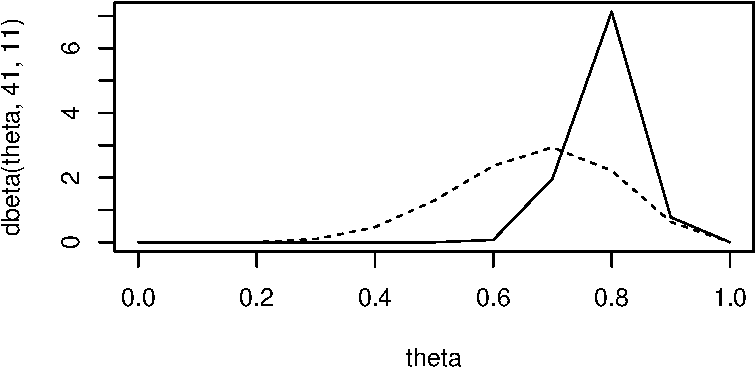
\includegraphics[keepaspectratio]{C1-L07_files/figure-pdf/C1-L07-3-1.pdf}}

Posterior probabilities

\begin{Shaded}
\begin{Highlighting}[]
\DecValTok{1} \SpecialCharTok{{-}} \FunctionTok{pbeta}\NormalTok{(}\FloatTok{0.25}\NormalTok{, }\DecValTok{41}\NormalTok{, }\DecValTok{11}\NormalTok{)}
\end{Highlighting}
\end{Shaded}

\begin{verbatim}
[1] 1
\end{verbatim}

\begin{Shaded}
\begin{Highlighting}[]
\CommentTok{\#[1] 1}
\DecValTok{1} \SpecialCharTok{{-}} \FunctionTok{pbeta}\NormalTok{(}\FloatTok{0.5}\NormalTok{, }\DecValTok{41}\NormalTok{, }\DecValTok{11}\NormalTok{)}
\end{Highlighting}
\end{Shaded}

\begin{verbatim}
[1] 0.9999926
\end{verbatim}

\begin{Shaded}
\begin{Highlighting}[]
\CommentTok{\#[1] 0.9999926}
\DecValTok{1} \SpecialCharTok{{-}} \FunctionTok{pbeta}\NormalTok{(}\FloatTok{0.8}\NormalTok{, }\DecValTok{41}\NormalTok{, }\DecValTok{11}\NormalTok{)}
\end{Highlighting}
\end{Shaded}

\begin{verbatim}
[1] 0.4444044
\end{verbatim}

\begin{Shaded}
\begin{Highlighting}[]
\CommentTok{\#[1] 0.4444044}
\end{Highlighting}
\end{Shaded}

Equal-tailed 95\% credible interval

\begin{Shaded}
\begin{Highlighting}[]
\FunctionTok{qbeta}\NormalTok{(}\FloatTok{0.025}\NormalTok{, }\DecValTok{41}\NormalTok{, }\DecValTok{11}\NormalTok{)}
\end{Highlighting}
\end{Shaded}

\begin{verbatim}
[1] 0.6688426
\end{verbatim}

\begin{Shaded}
\begin{Highlighting}[]
\CommentTok{\#[1] 0.6688426}
\FunctionTok{qbeta}\NormalTok{(}\FloatTok{0.975}\NormalTok{, }\DecValTok{41}\NormalTok{, }\DecValTok{11}\NormalTok{)}
\end{Highlighting}
\end{Shaded}

\begin{verbatim}
[1] 0.8871094
\end{verbatim}

\begin{Shaded}
\begin{Highlighting}[]
\CommentTok{\#[1] 0.8871094}
\end{Highlighting}
\end{Shaded}

95\% confidence that \(\theta_1\) is between 0.67 and 0.89

\begin{enumerate}
\def\labelenumi{\arabic{enumi}.}
\setcounter{enumi}{5}
\tightlist
\item
  Suppose the second student gets 24 questions right. What is the
  posterior distribution for \(\theta_2\)?
  \(\mathbb{P}r(\theta > 0.25)\)? \(\mathbb{P}r(\theta > 0.5)\)?
  \(\mathbb{P}r(\theta > 0.8)\)? What is the 95\% posterior credible
  interval for \(\theta_2\)
\end{enumerate}

\[
\text{Posterior} \sim \mathrm{Beta}(8 + 24, 4 + 40 - 24) = \mathrm{Beta}(32, 20)
\]

With a posterior mean of \(\frac{32}{32+20} = \frac{32}{52}\)

We can plot the posterior distribution with the prior

\begin{Shaded}
\begin{Highlighting}[]
\FunctionTok{plot}\NormalTok{(theta, }\FunctionTok{dbeta}\NormalTok{(theta, }\DecValTok{32}\NormalTok{, }\DecValTok{20}\NormalTok{), }\AttributeTok{type =} \StringTok{\textquotesingle{}l\textquotesingle{}}\NormalTok{)}
\FunctionTok{lines}\NormalTok{(theta, }\FunctionTok{dbeta}\NormalTok{(theta, }\DecValTok{8}\NormalTok{ ,}\DecValTok{4}\NormalTok{), }\AttributeTok{lty =} \DecValTok{2}\NormalTok{) }\CommentTok{\#Dashed line for prior}
\end{Highlighting}
\end{Shaded}

\pandocbounded{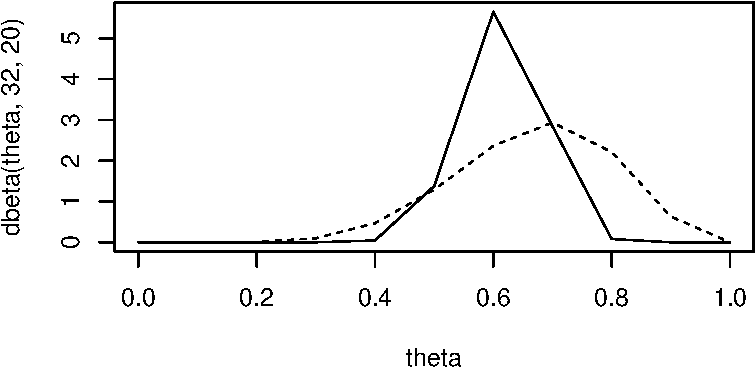
\includegraphics[keepaspectratio]{C1-L07_files/figure-pdf/C1-L07-6-1.pdf}}

Posterior probabilities

\begin{Shaded}
\begin{Highlighting}[]
\DecValTok{1} \SpecialCharTok{{-}} \FunctionTok{pbeta}\NormalTok{(}\FloatTok{0.25}\NormalTok{, }\DecValTok{32}\NormalTok{, }\DecValTok{20}\NormalTok{)}
\end{Highlighting}
\end{Shaded}

\begin{verbatim}
[1] 1
\end{verbatim}

\begin{Shaded}
\begin{Highlighting}[]
\CommentTok{\#[1] 1}
\DecValTok{1} \SpecialCharTok{{-}} \FunctionTok{pbeta}\NormalTok{(}\FloatTok{0.5}\NormalTok{, }\DecValTok{32}\NormalTok{, }\DecValTok{20}\NormalTok{)}
\end{Highlighting}
\end{Shaded}

\begin{verbatim}
[1] 0.9540427
\end{verbatim}

\begin{Shaded}
\begin{Highlighting}[]
\CommentTok{\#[1] 0.9540427}
\DecValTok{1} \SpecialCharTok{{-}} \FunctionTok{pbeta}\NormalTok{(}\FloatTok{0.8}\NormalTok{, }\DecValTok{32}\NormalTok{, }\DecValTok{20}\NormalTok{)}
\end{Highlighting}
\end{Shaded}

\begin{verbatim}
[1] 0.00124819
\end{verbatim}

\begin{Shaded}
\begin{Highlighting}[]
\CommentTok{\#[1] 0.00124819}
\end{Highlighting}
\end{Shaded}

Equal-tailed 95\% credible interval

\begin{Shaded}
\begin{Highlighting}[]
\FunctionTok{qbeta}\NormalTok{(}\FloatTok{0.025}\NormalTok{, }\DecValTok{32}\NormalTok{, }\DecValTok{20}\NormalTok{)}
\end{Highlighting}
\end{Shaded}

\begin{verbatim}
[1] 0.4808022
\end{verbatim}

\begin{Shaded}
\begin{Highlighting}[]
\CommentTok{\#[1] 0.4808022}
\FunctionTok{qbeta}\NormalTok{(}\FloatTok{0.975}\NormalTok{, }\DecValTok{32}\NormalTok{, }\DecValTok{20}\NormalTok{)}
\end{Highlighting}
\end{Shaded}

\begin{verbatim}
[1] 0.7415564
\end{verbatim}

\begin{Shaded}
\begin{Highlighting}[]
\CommentTok{\#[1] 0.7415564}
\end{Highlighting}
\end{Shaded}

95\% confidence that \(\theta_1\) is between 0.48 and 0.74

\begin{enumerate}
\def\labelenumi{\arabic{enumi}.}
\setcounter{enumi}{6}
\tightlist
\item
  What is the posterior probability that \(\theta_1 > \theta_2\)?
\end{enumerate}

i.e., that the first student has a better chance of getting a question
right than the second student?

Estimate by simulation: draw 1,000 samples from each and see how often
we observe \(\theta_1 > \theta_2\)

\begin{Shaded}
\begin{Highlighting}[]
\NormalTok{theta1 }\OtherTok{=} \FunctionTok{rbeta}\NormalTok{(}\DecValTok{100000}\NormalTok{, }\DecValTok{41}\NormalTok{, }\DecValTok{11}\NormalTok{)}
\NormalTok{theta2 }\OtherTok{=} \FunctionTok{rbeta}\NormalTok{(}\DecValTok{100000}\NormalTok{, }\DecValTok{32}\NormalTok{, }\DecValTok{20}\NormalTok{)}
\FunctionTok{mean}\NormalTok{(theta1 }\SpecialCharTok{\textgreater{}}\NormalTok{ theta2)}
\end{Highlighting}
\end{Shaded}

\begin{verbatim}
[1] 0.97429
\end{verbatim}

\begin{Shaded}
\begin{Highlighting}[]
\CommentTok{\#[1] 0.975}
\end{Highlighting}
\end{Shaded}

\chapter{Homework on Priors -
M2L7HW1}\label{homework-on-priors---m2l7hw1}

Bayesian Statistics: From Concept to Data Analysis

\hfill\break

\index{Maximum Likelihood Estimation}

\begin{tcolorbox}[enhanced jigsaw, bottomrule=.15mm, colbacktitle=quarto-callout-caution-color!10!white, leftrule=.75mm, bottomtitle=1mm, titlerule=0mm, title=\textcolor{quarto-callout-caution-color}{\faFire}\hspace{0.5em}{Caution}, rightrule=.15mm, toprule=.15mm, colback=white, left=2mm, toptitle=1mm, arc=.35mm, opacitybacktitle=0.6, coltitle=black, breakable, opacityback=0, colframe=quarto-callout-caution-color-frame]

Section omitted to comply with the Honor Code

\end{tcolorbox}

\chapter{Poisson Data - M3L8}\label{poisson-data---m3l8}

Bayesian Statistics: From Concept to Data Analysis

\hfill\break

\begin{marginfigure}

\centering{

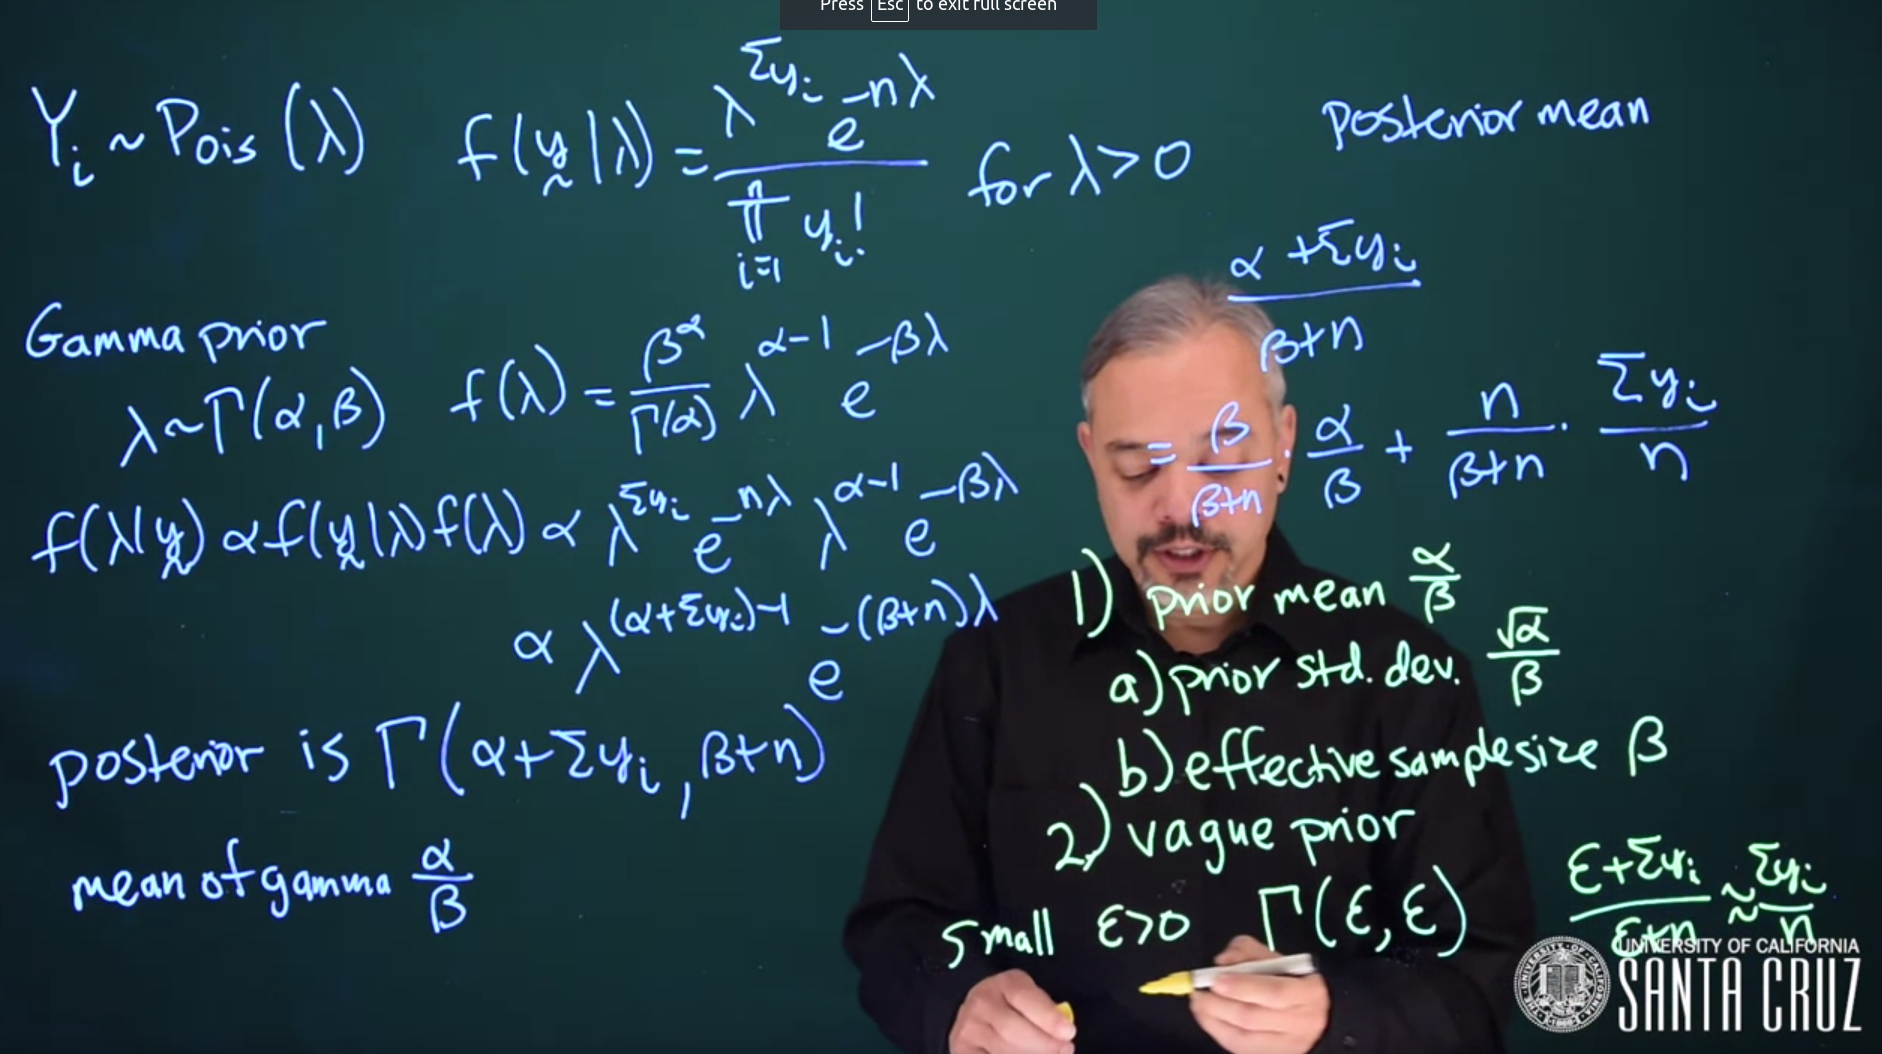
\includegraphics[width=53mm,height=\textheight,keepaspectratio]{images/c1l08-ss-01-poisson-data.png}

}

\caption{\label{fig-poisson-likelihood-gamma-prior}Poisson likelihood
with a Gamma prior}

\end{marginfigure}%

\phantomsection\label{exp-chocolate-chip}
\subsection{Poisson - Chocolate Chip
Cookie}\label{poisson---chocolate-chip-cookie}

In mass-produced chocolate chip cookies, they make a large amount of
dough; mix in a large number of chips; then chunk out the individual
cookies. In this process, the number of chips per cookie approximately
follows a \textbf{Poisson distribution}.

If we were to assume that chips have no volume, then this would be
exactly a \emph{Poisson process} and follow exactly a \emph{Poisson
distribution}. In practice, since chips are not that small, so they
follow approximately a Poisson distribution for the number of chips per
cookie.

\begin{equation}\phantomsection\label{eq-poisson}{
Y_i \sim \mathrm{Poisson}(\lambda)
}\end{equation}

{\marginnote{\begin{footnotesize}\textbf{What is the likelihood of the
data?}\end{footnotesize}}} The likelihood of the data is given by the
Poisson distribution.

\[
\begin{aligned}
{\color{red}f(y \mid \lambda) = \frac{\lambda^{\sum{y_i}}e^{-n\lambda}}{\prod_{i = 1}^n{y_i!}}} \quad \forall (\lambda > 0) && \text{ Poisson Likelihood } 
\end{aligned}
\]

{\marginnote{\begin{footnotesize}\textbf{What type of prior should we
put on} \(\lambda\) ?\end{footnotesize}}} It would be convenient if we
could put a \emph{conjugate prior}. What distribution looks like
\(\lambda\) raised to a power and \(e\) raised to a negative power?

For this, we're going to use a Gamma prior.

\begin{equation}\phantomsection\label{eq-gamma-prior}{
\begin{aligned} \lambda &\sim \mathrm{Gamma}(\alpha, \beta) && \text{Gamma Prior} \\ 
\color{green}{ f(\lambda)} &= \color{green}{\frac{\beta^\alpha}{\Gamma(\alpha)}\lambda^{\alpha - 1}e^{-\beta\lambda}} && \text{subst. Gamma PDF} \end{aligned}
}\end{equation}

{\marginnote{\begin{footnotesize}\textbf{What is the
posterior?}\end{footnotesize}}} We can use Bayes theorem to find the
posterior.

\begin{equation}\phantomsection\label{eq-posterior}{
\begin{aligned} {\color{blue}f(\lambda \mid y)} &\propto \color{red}{ f(y \mid \lambda)} \color{green}{ f(\lambda)} && \text{Bayes without the denominator} \\ 
&\propto \color{red}{\lambda^{\sum{y_i}}e^{-n\lambda}}\color{green}{\lambda^{\alpha - 1}e^{-\beta \lambda} } && \text{subst. Likelihood and Prior} \\ 
& \propto { \color{blue} \lambda^{\alpha + \sum{y_i} - 1}e^{-(\beta + n)\lambda} } && \text{collecting terms} \\ 
& \propto { \color{blue} \mathrm{Gamma}(\alpha + \sum{y_i}, \beta + n)}
\end{aligned} 
}\end{equation}

{\marginnote{\begin{footnotesize}\textbf{What is the posterior
distribution?}\end{footnotesize}}} The posterior is a Gamma distribution
with parameters \(\alpha + \sum{y_i}\) and \(\beta + n\).

Thus we can see that the posterior is a Gamma Distribution

\begin{equation}\phantomsection\label{eq-posterior-gamma}{
\lambda \mid y \sim \mathrm{Gamma}(\alpha + \sum{y_i}, \beta + n)
}\end{equation}

{\marginnote{\begin{footnotesize}\textbf{What is the posterior
mean?}\end{footnotesize}}} The posterior mean of a Gamma distribution is
given by

\hl{The mean of Gamma under this parameterization is:}
\(\frac{\alpha}{\beta}\)

The posterior mean is going to be

\begin{equation}\phantomsection\label{eq-posterior-mean}{
\begin{aligned}
{\color{blue}\mu_{\lambda}} &= \frac{\alpha + \sum{y_i}}{\beta + n} && \text{(Posterior Mean)} \\
posterior_{\mu} 
&= \frac{\alpha + \sum{y_i}}{\beta + n} \\
&= \frac{\beta}{\beta + n}\frac{\alpha}{\beta} + \frac{n}{\beta + n}\frac{\sum{y_i}}{n} \\
& \propto  \beta \cdot \mu_\text{prior} + n\cdot \mu_\text{data}
\end{aligned}
}\end{equation}

{\marginnote{\begin{footnotesize}\textbf{What is the posterior
variance?}\end{footnotesize}}} The posterior variance of a Gamma
distribution is given by

As you can see here the posterior mean of the Gamma distribution is also
the weighted average of the prior mean and the data mean.

\index{MCMC!effective sample size} Therefore, \hl{the effective sample
size (ESS) of the Gamma prior is} \(\beta\)

\begin{tcolorbox}[enhanced jigsaw, bottomrule=.15mm, colbacktitle=quarto-callout-tip-color!10!white, leftrule=.75mm, bottomtitle=1mm, titlerule=0mm, title=\textcolor{quarto-callout-tip-color}{\faLightbulb}\hspace{0.5em}{Prior Elicitation of Gamma Hyper-parameters}, rightrule=.15mm, toprule=.15mm, colback=white, left=2mm, toptitle=1mm, arc=.35mm, opacitybacktitle=0.6, coltitle=black, breakable, opacityback=0, colframe=quarto-callout-tip-color-frame]

Here are two strategies for choose the \emph{hyper-parameters}
\(\alpha\) and \(\beta\)

\begin{enumerate}
\def\labelenumi{\arabic{enumi}.}
\tightlist
\item
  \hl{An \emph{informative prior} with a prior mean guess of}
  \(\mu=\frac{a}{b}\) e.g.~what is the average number of chips per
  cookie?

  \begin{itemize}
  \tightlist
  \item
    Next we need another piece of knowledge to pinpoint both parameters.
  \item
    \hl{Can you estimate the error for the mean? I.e. what do you think
    the \emph{standard deviation} is? Since for the Gamma prior}
  \item
    \hl{What is the effective sample size} \(\text{ESS}=\beta\) ?
  \item
    \hl{How many units of information do you think we have in our prior
    v.s. our data points ?} \(\sigma = \frac{ \sqrt{\alpha} }{\beta}\)
  \end{itemize}
\item
  \hl{A \emph{vague prior} \index{prior!vague} refers to one that's
  relatively flat across much of the space.}

  \begin{itemize}
  \tightlist
  \item
    For a \emph{Gamma prior} we can choose
    \(\Gamma(\varepsilon, \varepsilon)\) where \(\varepsilon\) is small
    and strictly positive. This would create a distribution with a
    \(\mu = 1\) and a huge \(\sigma\) stretching across the whole space.
    And the \emph{effective sample size} will also be \(\varepsilon\)
    Hence the posterior will be largely driven by the data and very
    little by the prior.
  \end{itemize}
\end{enumerate}

\end{tcolorbox}

The first strategy with a mean and an ESS will be used in numerous
models going forward so it is best to remember these two strategies!

\chapter{Homework on Poisson Data -
M3L8HW1}\label{homework-on-poisson-data---m3l8hw1}

Bayesian Statistics: From Concept to Data Analysis

\hfill\break

\begin{tcolorbox}[enhanced jigsaw, bottomrule=.15mm, colbacktitle=quarto-callout-caution-color!10!white, leftrule=.75mm, bottomtitle=1mm, titlerule=0mm, title=\textcolor{quarto-callout-caution-color}{\faFire}\hspace{0.5em}{Caution}, rightrule=.15mm, toprule=.15mm, colback=white, left=2mm, toptitle=1mm, arc=.35mm, opacitybacktitle=0.6, coltitle=black, breakable, opacityback=0, colframe=quarto-callout-caution-color-frame]

Section omitted to comply with the Honor Code

\end{tcolorbox}

\chapter{Beta Bernoulli - M3L8HW2}\label{beta-bernoulli---m3l8hw2}

Bayesian Statistics: From Concept to Data Analysis

\hfill\break

\begin{tcolorbox}[enhanced jigsaw, bottomrule=.15mm, colbacktitle=quarto-callout-caution-color!10!white, leftrule=.75mm, bottomtitle=1mm, titlerule=0mm, title=\textcolor{quarto-callout-caution-color}{\faFire}\hspace{0.5em}{Caution}, rightrule=.15mm, toprule=.15mm, colback=white, left=2mm, toptitle=1mm, arc=.35mm, opacitybacktitle=0.6, coltitle=black, breakable, opacityback=0, colframe=quarto-callout-caution-color-frame]

Section omitted to comply with the Honor Code

\end{tcolorbox}

\chapter{M4L9 - Exponential Data}\label{m4l9---exponential-data}

Bayesian Statistics: From Concept to Data Analysis

\hfill\break

\section{Exponential Data}\label{sec-exponential-data}

\begin{marginfigure}

\centering{

\includegraphics[width=53mm,height=\textheight,keepaspectratio]{images/c1l09-ss-01-exponential-data.png}

}

\caption{\label{fig-exponential-likelihood-gamma-prior}Exponential
likelihood with a Gamma prior}

\end{marginfigure}%

{\marginnote{\begin{footnotesize}Time between buses\end{footnotesize}}}
Suppose you're waiting for a bus that you think comes on average once
every 10 minutes, but you're not sure exactly how often it comes.

\begin{equation}\phantomsection\label{eq-exponential-RV}{
Y \sim \mathrm{Exp}(\lambda)
}\end{equation}

Your waiting time has a prior expectation of \(\frac{1}{\lambda}\)

The \emph{Gamma distribution} is conjugate for an \emph{Exponential
likelihood}. We need to specify a prior, or a particular Gamma in this
case. If we think that the buses come on average every ten minutes,
that's a rate of one over ten.

\[ 
prior_{\mu} = \frac{1}{10} 
\]

Thus, we'll want to specify a gamma distribution so that the first
parameter divided by the second parameter is \({1 \over 10}\)

We can now think about our variability. Perhaps you specify

\[
\mathrm{Gamma}(100, 1000)
\]

This will indeed have a prior mean of \({1 \over 10}\) and it'll have a
standard deviation of \({1 \over 100}\). If you want to have a rough
estimate of our mean plus or minus two standard deviations then we have
the following

\[
0.1 \pm 0.02
\]

Suppose that we wait for 12 minutes and a bus arrives. Now you want to
update your posterior for \(\lambda\) about how often this bus will
arrive.

\[
f(\lambda \mid y) \propto f(y\mid \lambda)f(\lambda)
\]

\[
f(\lambda \mid y) \propto \lambda e^{-\lambda y}\lambda^{\alpha - 1}e^{-\beta \lambda}
\]

\[
f(\lambda \mid y)  \propto \lambda^{(\alpha + 1) - 1}e^{-(\beta + y)\lambda}
\]

\[
\lambda \mid y \sim \mathrm{Gamma}(\alpha + 1, \beta + y)
\]

Plugging in our particular prior gives us a posterior for \(\lambda\)
which is

\[
\lambda \mid y \sim \mathrm{Gamma}(101, 1012)
\]

Thus our posterior mean is going to be \(\frac{101}{1012} = 0.0998.\)

This one observation does not contain a lot of data under this
likelihood. When the bus comes and it takes 12 minutes instead of 10, it
barely shifts our posterior mean up.

One data point does not have a big impact here.

\begin{exercise}[]\protect\hypertarget{exr-gamma-exp-1}{}\label{exr-gamma-exp-1}

We can generalize the result from the lesson to more than one data
point.

\end{exercise}

Suppose

\[
Y_1, \ldots, Y_n \stackrel{iid}\sim Exp(\lambda)=\lambda e^{-\lambda x}\mathbb{I}_{x\ge0}
\]

with mean

\[
\mathbb{E}[Y]=\frac{1}{\lambda}
\]

and assume a

\[
f(\lambda)= \mathrm{Gamma}(\alpha, \beta) \qquad (\text{prior for }\lambda)
\]

The likelihood is then:

\[
f(y \mid \lambda) = \prod \lambda e^{-\lambda x}\mathbb{I}_{x\ge0} =  \lambda ^ n e^{− \lambda \sum y_i}\cdot1
\]

and we can follow the same steps from the lesson to obtain the posterior
distribution (try to derive it yourself):

\[
\lambda \mid y ∼ \mathrm{Gamma}(\alpha + n, \beta + \sum y_i)
\]

\index{MCMC!effective sample size} What is the prior effective sample
size (ess) in this model?

\begin{solution}
The data sample size \(n\) is added to \(\alpha\) to update the first
parameter. Thus \(\alpha\) can be interpreted as the sample size
equivalent in the prior.
\end{solution}

It might be helpful to think about a related problems\ldots{}

\begin{enumerate}
\def\labelenumi{\arabic{enumi}.}
\tightlist
\item
  We are waiting at a bus stop with 1 bus line, the information at the
  bus stop say that the bus comes on average every 10 minutes at this
  time. How long do we expect to wait for the bus?
\item
  what if we have waited for k minutes and the bus has not arrived yet?
  How long do we expect to wait for the bus?
\item
  While we are waiting more people arrive at the bus stop. You notice
  the bus stop features a digital counter and a display with long term
  mean E and V variance of the number of people at the bus stop. Can we
  use this information to get a better estimate of our bus arrival time?
\item
  If we wait at a bus stop with K different bus lines each with the same
  lambda, and we see a L people waiting. Can we get a better estimate of
  our bus arrival time?
\item
  What if more people come. And we know the mean and variance of the
  people waiting at the bus stop?
\item
  What if a different bus line arrives and the number of people waiting
  is now M?
\item
  What if each bus line has a different lambda, but we know the mean and
  variance of the people waiting at the bus stop?
\end{enumerate}

\chapter{Homework on Exponential Data -
M4L9HW1}\label{homework-on-exponential-data---m4l9hw1}

Bayesian Statistics: From Concept to Data Analysis

\hfill\break

\begin{tcolorbox}[enhanced jigsaw, bottomrule=.15mm, colbacktitle=quarto-callout-caution-color!10!white, leftrule=.75mm, bottomtitle=1mm, titlerule=0mm, title=\textcolor{quarto-callout-caution-color}{\faFire}\hspace{0.5em}{Caution}, rightrule=.15mm, toprule=.15mm, colback=white, left=2mm, toptitle=1mm, arc=.35mm, opacitybacktitle=0.6, coltitle=black, breakable, opacityback=0, colframe=quarto-callout-caution-color-frame]

Section omitted to comply with the Honor Code

\end{tcolorbox}

\chapter{Normally distributed Data -
M4L10}\label{normally-distributed-data---m4l10}

Bayesian Statistics: From Concept to Data Analysis

\hfill\break

It is often pointed out that Normally distributed data is not very
commonly encountered in the real world. However, when it comes to
modeling, using a normal RV is second to none.(Hoff 2009, 75). The
Section~\ref{sec-cl-theorem} {\marginnote{\begin{footnotesize}Central
Limit Theorem\end{footnotesize}}} is the primary reason that the normal
is a good approximation if there are enough IID
{\marginnote{\begin{footnotesize}Independent Identically
Distributed\end{footnotesize}}} samples. We will look at two types of
\emph{conjugate normal priors}, and in the next unit we will consider
two more uninformative priors for Normally distributed data.

\href{https://real-statistics.com/bayesian-statistics/bayesian-statistics-normal-data/conjugate-priors-normal-distribution/}{Charles
Zaiontz} provides pro types of conjugate priors for normally distributed
data:

\begin{enumerate}
\def\labelenumi{\arabic{enumi}.}
\tightlist
\item
  Mean unknown and variance known.
\item
  Variance unknown and mean known and
\item
  Mean and variance are unknown
\end{enumerate}

In each case, the \textbf{unknown} refer to \emph{population
statistics}. Since we are able to estimate \emph{sample parameters} such
as the mean and variance quite easily. A key question to consider is how
well does our posterior distribution of the parameter representative of
the unknown population statistic?

{\marginnote{\begin{footnotesize}\textbf{How good is our estimate of the
known population statistic?}\end{footnotesize}}}

Ideally, I will update the notes below with proofs of conjugate, prior
and posterior and marginal distribution.

Some of the proofs are in \href{handouts/L10_supp.pdf}{here} as well

\begin{itemize}
\tightlist
\item
  See (Gelman et al. 2013, sec. 3.2) for Normal data with a
  noninformative prior distribution
\item
  See (Gelman et al. 2013, sec. 3.2) for Normal data with a conjugate
  prior distribution
\end{itemize}

\section{Normal Likelihood with known
variance}\label{sec-normal-likelihood-with-unknown-mean}

\begin{marginfigure}

\centering{

\includegraphics[width=53mm,height=\textheight,keepaspectratio]{images/c1l10-ss-01-normal-data.png}

}

\caption{\label{fig-normal-with-known-variance-prior}Normal likelihood
with variance known}

\end{marginfigure}%

Note: this material is also covered in (Hoff 2009, sec. 5.2)
\index{distribution!Normal!known variance}

Let's suppose the \textbf{standard deviation or variance} \(\sigma^2\)
is known and we're only interested in learning about the mean. This is a
situation that often arises in monitoring industrial production
processes.

\begin{equation}\phantomsection\label{eq-normal-RV-known-mean-variance}{
X_i \stackrel{iid}\sim \mathcal{N}(\mu, \sigma^2)
}\end{equation}

It turns out that the Normal distribution is conjugate for itself when
looking for the mean parameter

Prior

\begin{equation}\phantomsection\label{eq-normal-conjugate-prior}{
\mu \sim \mathcal{N}(m_0,S_0^2)
}\end{equation}

By Bayes rule:

\[
f(\mu \mid x ) \propto f(x \mid \mu)f(\mu)
\]

\begin{equation}\phantomsection\label{eq-normal-posterior}{
\mu \mid x \sim \mathcal{N} \left (\frac{\frac{n\bar{x}}{\sigma_0^2} + \frac{m_0}{s_0^2} }{\frac{n}{\sigma_0^2} +\frac{1}{s_0^2}}, \frac{1}{\frac{n}{\sigma_0^2} + \frac{1}{s_0^2}}\right )
}\end{equation}

where:

\begin{itemize}
\tightlist
\item
  \(n\) is the sample size
\item
  \(\bar{x}=\frac{1}{n}\sum x_i\) is the sample mean
\item
  \(\sigma =\frac{1}{n} \sum (x_i-\bar{x})^2\) is the sample variance
\item
  indexing parameters with 0 seems to be a convention that they are from
  the prior:
\item
  \(s_0\) is the prior variance
\item
  \(m_0\) is the prior mean
\end{itemize}

Let's look at the posterior mean

\begin{equation}\phantomsection\label{eq-normal-posterior-mean-ess}{
\begin{aligned}
posterior_{\mu} &= \frac{ 
          \frac{n}{\sigma_0^2}}
       {\frac{n}{\sigma_0^2}s + \frac{1}{s_0^2}}\bar{x} +     
          \frac{ \frac{1}{s_0^2} }{ \frac{n}{\sigma_0^2} + \frac{1}{s_0^2}
        }m \\ 
&= \frac{n}{n + \frac{\sigma_0^2}{s_0^2} }\bar{x} + \frac{ \frac{\sigma_0^2}{s_0^2} }{n + \frac{\sigma_0^2}{s_0^2}}m
\end{aligned}
}\end{equation}

\begin{tcolorbox}[enhanced jigsaw, bottomrule=.15mm, colbacktitle=quarto-callout-warning-color!10!white, leftrule=.75mm, bottomtitle=1mm, titlerule=0mm, title=\textcolor{quarto-callout-warning-color}{\faExclamationTriangle}\hspace{0.5em}{Warning}, rightrule=.15mm, toprule=.15mm, colback=white, left=2mm, toptitle=1mm, arc=.35mm, opacitybacktitle=0.6, coltitle=black, breakable, opacityback=0, colframe=quarto-callout-warning-color-frame]

should we use n-1 in the sample variance?

\end{tcolorbox}

Thus we see, that the posterior mean is a \textbf{weighted average} of
the prior mean and the data mean. And indeed that the \textbf{effective
sample size} for this prior is the ratio of the variance for the data to
the variance in the prior.

\begin{equation}\phantomsection\label{eq-normal-prior-ESS}{
Prior\ ESS= \frac{\sigma_0^2}{s_0^2}
}\end{equation}

This makes sense, because the larger the variance of the prior, the less
information that's in it.

The \textbf{marginal distribution} for Y is

\begin{equation}\phantomsection\label{eq-normal-marginal}{
\mathcal{N}(m_0, s_0^2 + \sigma^2)
}\end{equation}

\subsection{Prior (and posterior) predictive
distribution}\label{prior-and-posterior-predictive-distribution}

The \textbf{prior (and posterior) predictive distribution} for data is
particularly simple in the \emph{conjugate normal model}
\index{conjugate normal model}.

If \[
y \mid \theta \sim \mathcal{N}(\theta,\sigma^2)
\] and \[
\theta \sim \mathcal{N}(m, s_0^2)
\]

then the \textbf{marginal distribution} for \(Y\), obtained as

\begin{equation}\phantomsection\label{eq-normal-predictive-distribution}{
\int f(y,\theta) d\theta = \mathcal{N}(m_0,s_0^2)
}\end{equation}

\begin{example}[]\protect\hypertarget{exm-normal-predictive}{}\label{exm-normal-predictive}

Suppose your data are normally distributed with \(\mu=\theta\) and
\(\sigma^2=1\).

\[
y \mid \theta \sim \mathcal{N}(\theta,1)
\]

You select a normal prior for \(\theta\) with mean 0 and variance 2.

\[
\theta \sim \mathcal{N}(0, 2)
\]

Then the \textbf{prior predictive distribution} for one data point would
be \(N(0, a)\). What is the value of \(a\)?

Since, \(m_0 =0,\) and \(s^2_0=2\) and \(\sigma^2=1\), the predictive
distribution is \(N(0,2+1)\).

\end{example}

\section{Normal likelihood with expectation and variance
unknown}\label{sec-normal-likelihood-with-expectation-and-variance-unknown}

\begin{marginfigure}

\centering{

\includegraphics[width=53mm,height=\textheight,keepaspectratio]{images/c1l10-ss-02-normal-data.png}

}

\caption{\label{fig-normal-with-unknown-variance-prior}Normal likelihood
with a unknown variance}

\end{marginfigure}%

\begin{tcolorbox}[enhanced jigsaw, bottomrule=.15mm, colbacktitle=quarto-callout-tip-color!10!white, leftrule=.75mm, bottomtitle=1mm, titlerule=0mm, title=\textcolor{quarto-callout-tip-color}{\faLightbulb}\hspace{0.5em}{Challenging}, rightrule=.15mm, toprule=.15mm, colback=white, left=2mm, toptitle=1mm, arc=.35mm, opacitybacktitle=0.6, coltitle=black, breakable, opacityback=0, colframe=quarto-callout-tip-color-frame]

This section is challenging.

\begin{itemize}
\tightlist
\item
  The updating derivation is skipped,
\item
  the posterior
\item
  updating rule values are introduced without motivations and
  explanation.
\item
  The model is also the most complicated in the course, the note at the
  end says this can be extended hierarchically if we want to specify
  hyper priors for \(m\), \(w\) and \(\beta\)
\item
  Other text discuss this case using a inverse chi squared distribution
\end{itemize}

If we can understand the model the homework is going to make sense. Also
this is probably the level needed for the other courses in the
specialization.

It can help to review some of the books:

\begin{itemize}
\tightlist
\item
  See (Hoff 2009, sec. 5.3) which has some R examples.
\item
  See (Gelman et al. 2013, sec. 5)
\end{itemize}

\end{tcolorbox}

\index{model!hierarchical}
\index{distribution!Normal!unknown mean and variance} \hl{If both $\mu$
and $\sigma^2$ are unknown, we can specify a \textbf{conjugate prior} in
a \textbf{hierarchical fashion}.}

\[
X_i \mid \mu, \sigma^2 \stackrel{iid}\sim \mathcal{N}(\mu, \sigma^2) \qquad \text{(the data given the params) }
\]

\begin{itemize}
\tightlist
\item
  This is the level 1 hierarchically model - \(X_i\) model our
  observations.
\item
  We state on the left, that the RV X is conditioned on the \(\mu\) and
  \(\sigma^2\).
\item
  But the variables \(\mu\) and \(\sigma^2\) are unknown population
  statistics which we will need to infer from the data. We can call them
  latent variables.
\end{itemize}

Next we add a prior from \(\mu\) conditional on the value for
\(\sigma^2\)

\[
\mu \mid \sigma^2 \sim \mathcal{N}(m, \frac{\sigma^2}{w}) \qquad \text{(prior of the mean conditioned on the variance)}
\]

where:

\begin{itemize}
\tightlist
\item
  \(w\) is going to be the ratio of \(\sigma^2\) and some variance for
  the Normal distribution. This is the \textbf{effective sample size of
  the prior}.
\item
  Why is the mean conditioned on the variance. We can have a model where
  they are independent too?
\item
  later on (in the homework) we are told that w can express the
  confidence in the prior.
\item
  I think this means that Since this is a knowledge of m, i.e.~giving
  \(w\) a weight of 1/10 expresses that we value\\
\item
  Perhaps this is due to \href{@sec-cl-theorem}{Central Limit Theorem} ?
\item
  This is level 2 of the model
\end{itemize}

Finally, the last step is to specify a prior for \(\sigma^2\). The
conjugate prior here is an inverse gamma distribution with parameters
\(\alpha\) and \(\beta\).

\[
\sigma^2 \sim \mathrm{Gamma}^{-1}(\alpha, \beta)  \qquad \text{prior of the variance}
\]

After many calculations\ldots{} we get the posterior distribution

\begin{equation}\phantomsection\label{eq-normal-cong-gamma-posterior}{
\sigma^2 \mid x \sim \mathrm{Gamma}^{-1}(\alpha + \frac{n}{2}, \beta + \frac{1}{2}\sum_{i = 1}^n{(x-\bar{x}^2 + \frac{nw}{2(n+2)}(\bar{x} - m)^2)})
}\end{equation}

\begin{equation}\phantomsection\label{eq-normal-cong-gamma-mean-posterior-dist}{
\mu \mid \sigma^2,x \sim \mathcal{N}(\frac{n\bar{x}+wm}{n+w}, \frac{\sigma^2}{n + w}) 
}\end{equation}

Where the posterior mean can be written as the \emph{weighted average}
of the \emph{prior mean} and the \emph{data mean}.

\begin{equation}\phantomsection\label{eq-normal-cong-gamma-mean-posterior-weighted-average}{
\frac{n\bar{x}+wm}{n+w} = \frac{w}{n + w}m + \frac{n}{n + w}\bar{x} \qquad \text{post. mean}
}\end{equation}

In some cases, we only care about \(\mu\). We want some inference on
\(\mu\) and we may want it such that it does not depend on \(\sigma^2\).
We can marginalize that \(\sigma^2\) integrating it out. The posterior
for \(\mu\) marginally follows a \(t\) distribution.

\[
\mu \mid x \sim t
\]

Similarly, the posterior predictive distribution also is a \(t\)
distribution.

Finally, note that we can extend this in various directions, this can be
extended to the multivariate normal case that requires matrix vector
notations and can be extended hierarchically if we want to specify
priors for \(m, w, \beta\)

\chapter{Homework on Normal Data -
M4L10HW1}\label{homework-on-normal-data---m4l10hw1}

Bayesian Statistics: From Concept to Data Analysis

\hfill\break

\begin{tcolorbox}[enhanced jigsaw, bottomrule=.15mm, colbacktitle=quarto-callout-caution-color!10!white, leftrule=.75mm, bottomtitle=1mm, titlerule=0mm, title=\textcolor{quarto-callout-caution-color}{\faFire}\hspace{0.5em}{Caution}, rightrule=.15mm, toprule=.15mm, colback=white, left=2mm, toptitle=1mm, arc=.35mm, opacitybacktitle=0.6, coltitle=black, breakable, opacityback=0, colframe=quarto-callout-caution-color-frame]

Section omitted to comply with the Honor Code

\end{tcolorbox}

\chapter{Non-Informative Priors -
M4L11}\label{non-informative-priors---m4l11}

Bayesian Statistics: Techniques and Models

\hfill\break

\section{Non-Informative Priors}\label{sec-non-informative-priors}

\begin{marginfigure}

\centering{

\includegraphics[width=53mm,height=\textheight,keepaspectratio]{images/c1l11-ss-01-non-informative-priors.png}

}

\caption{\label{fig-non-informative-priors}Non-Informative Priors}

\end{marginfigure}%

\index{prior!non-informative} We've seen examples of choosing priors
that contain a significant amount of information. We've also seen some
examples of choosing priors where we're attempting to not put too much
information in to keep them vague.

Another approach is referred to as objective Bayesian statistics or
inference where we explicitly try to minimize the amount of information
that goes into the prior.

This is an attempt to have the data have maximum influence on the
posterior

Let's go back to coin flipping

\[
Y_i \sim B(\theta)
\]

How do we minimize our prior information in \(\theta\)? One obvious
intuitive approach is to say that all values of \(\theta\) are equally
likely. So we could have a prior for \(\theta\) which follows a uniform
distribution on the interval \([0, 1]\)

Saying all values of \(\theta\) are equally likely \textbf{seems} like
it would have no information in it.

Recall however, that a \(Uniform(0, 1)\) is the same as \(Beta(1, 1)\)

The effective sample size of a beta prior is the sum of its two
parameters. So in this case, it has an effective sample size of 2. This
is equivalent to data, with one head and one tail already in it.

So this is not a completely non-informative prior.

We could think about a prior that has less information. For example
\(\mathrm{Beta}(\tfrac{1}{2}, \tfrac{1}{2})\), this would have half as
much information with an effective sample size of one.

We can take this even further. Think about something like
\(\mathrm{Beta}(0.001, 0.001)\) This would have much less information,
with the effective sample size fairly close to zero. In this case, the
data would determine the posterior and there would be very little
influence from the prior.

\subsection{Improper priors}\label{sec-improper-priors}

\index{prior!improper} \index{Improper prior} Can we go even further? We
can think of the limiting case. Let's think of \(Beta(0,0)\), what would
that look like?

\[
f(\theta) \propto \theta^{-1}(1-\theta)^{-1}
\]

This is not a proper density. If you integrate this over \((0,1)\),
you'll get an infinite integral, so it's not a true density in the sense
of it not integrating to 1.

There's no way to normalize it, since it has an infinite integral. This
is what we refer to as an improper prior.

It's improper in the sense that it doesn't have a proper density. But
it's not necessarily improper in the sense that we can't use it. If we
collect data, we use this prior and as long as we observe one head and
one tail, or \textbf{at least one success and one failure}. Then we can
get a posterior

\[
f(\theta\mid y) \propto \theta^{y-1}(1-\theta)^{n-y-1} \sim Beta(y, n-y)
\]

With a posterior mean of \(\frac{y}{n} =\hat{\theta}\), which you should
recognize as the maximum likelihood estimate. So by using this improper
prior, we get a posterior which gives us point estimates exactly the
same as the frequentist approach. \index{Maximum Likelihood Estimation}

But in this case, we can also think of having a full posterior. From
this, we can make interval statements, and probability statements, and
we can actually find an interval and say that there's \(95\%\)
probability that \(\theta\) is in this interval. This is not something
you can do under the frequentist approach even though we may get the
same exact interval.

\subsection{Statements about improper
priors}\label{sec-statements-about-improper-priors}

Improper priors are okay as long as the posterior itself is proper.
There may be some mathematical things that need to be checked and you
may need to have certain restrictions on the data. In this case, we
needed to make sure that we observed at least one head and one tail to
get a proper posterior.

But as long as the posterior is proper, we can go forwards and do
Bayesian inference even with an improper prior.

The second point is that for many problems there does exist a prior,
typically an improper prior that will lead to the same point estimates
as you would get under the frequentist paradigm. So we can get very
similar results, results that are fully dependent on the data, under the
Bayesian approach.

But in this case, we can also continue to have a posterior and make
posterior interval estimates and talk about the posterior probabilities
of the parameter.

\subsection{Normal Case}\label{sec-normal-case}

Another example is thinking about the normal case.

\begin{equation}\phantomsection\label{eq-normal-case}{
Y_i \stackrel{iid}\sim \mathcal{N}(\mu, \sigma^2)
}\end{equation}

Let's start off by assuming that \(\sigma^2\) is known and we'll just
focus on the mean \(\mu\).

\index{prior!vague} We can think about a vague prior like before and say
that:

\begin{equation}\phantomsection\label{eq-vague-prior-normal}{
\mu \sim N(0, 1000000^2)
}\end{equation}

This would just spread things out across the real line. That would be a
fairly non-informative prior covering a lot of possibilities. We can
then think about taking the limit, what happens if we let the variance
go to \(\infty\). In that case, we're spreading out this distribution
across the entire real number line. We can say that the density is just
a constant across the whole real line.

\[
f(\mu) \propto 1
\]

This is an improper prior because if you integrate the real line you get
an infinite answer. However, if we go ahead and find the posterior

\[
f(\mu \mid y) \propto f(y \mid \mu) f(\mu) \propto \exp \left (-\frac{1}{2\sigma^2}\sum{(y_i - \mu)^2} \right ) (1)
\]

\[
f(\mu \mid y) \propto \exp(-\frac{1}{2\sigma^2/n}(\mu - \bar{y})^2)
\]

\[
\mu \mid y \sim \mathcal{N}(\bar{y}, \frac{\sigma^2}{n})
\]

This should look just like the maximum likelihood estimate.

\subsection{Normal with unknown
Variance}\label{sec-normal-unknown-variance}

In the case that \(\sigma^2\) is unknown, the standard non-informative
prior is

\[
f(\sigma^2) \propto \frac{1}{\sigma^2}
\]

\[
\sigma^2 \sim \Gamma^{-1}(0,0)
\]

\index{prior!improper} This is an improper prior and it's uniform on the
log scale of \(\sigma^2\).

In this case, we'll end up with a posterior for \(\sigma^2\)

\[
\sigma^2 \mid y \sim \Gamma^{-1}\left (\frac{n-1}{2}, \frac{1}{2}\sum{(y_i - \bar{y})^2}\right)
\]

This should also look reminiscent of the quantities we get as a
frequentist. For example, the samples standard deviation

\section{Jeffrey's Prior}\label{sec-jeffreys-prior}

\begin{marginfigure}

\centering{

\includegraphics[width=53mm,height=\textheight,keepaspectratio]{images/c1l11-ss-02-jeffreys-priors.png}

}

\caption{\label{fig-jeffreys-priors}Jeffrey's Prior}

\end{marginfigure}%

Choosing a uniform prior depends upon the particular parameterization.

Suppose I used a prior which is uniform on the log scale for
\(\sigma^2\)

\[
f(\sigma^2) \propto \frac{1}{\sigma^2}
\]

Suppose somebody else decides, that they just want to put a uniform
prior on \(\sigma^2\) itself.

\[
f(\sigma^2) \propto 1
\]

These are both uniform on certain scales or certain parameterizations,
but they are different priors. So when we compute the posteriors, they
will be different as well.

The key thing is that uniform priors are not invariant with respect to
transformation. Depending on how you parameterize the problem, you can
get different answers by using a uniform prior

One attempt to round this out is to use \textbf{Jeffreys Prior}

\index{prior!Jeffreys} Jeffrey's Prior is defined as the following

\[
f(\theta) \propto \sqrt{\mathcal{I(\theta)}}
\]

Where \(\mathcal{I}(\theta)\) is the fisher information of \(\theta\).

In most cases, this will be an \textbf{improper prior}.

\begin{figure}[H]

{\centering \includegraphics[width=53mm,height=\textheight,keepaspectratio]{images/bio-Harold-Jeffreys.jpg}

}

\caption{Harold Jeffreys}

\end{figure}%

\begin{tcolorbox}[enhanced jigsaw, bottomrule=.15mm, colbacktitle=quarto-callout-tip-color!10!white, leftrule=.75mm, bottomtitle=1mm, titlerule=0mm, title=\textcolor{quarto-callout-tip-color}{\faLightbulb}\hspace{0.5em}{Historical Note on Sir Harold Jeffreys}, rightrule=.15mm, toprule=.15mm, colback=white, left=2mm, toptitle=1mm, arc=.35mm, opacitybacktitle=0.6, coltitle=black, breakable, opacityback=0, colframe=quarto-callout-tip-color-frame]

Jeffreys' Prior is due to Sir Harold Jeffreys (1891-1989) a British
geophysicist who who used sophisticated mathematical models to study the
Earth and solar system. His hypotheses were uncertain, requiring
revision in the face of incoming results, Jeffreys tried to construct a
formal theory of scientific reasoning based on Bayesian probability. He
made significant contributions to mathematics and statistics. His book,
Theory of Probability (Jeffreys 1983), first published in 1939, played
an important role in the revival of the objective Bayesian view of
probability.

Inductive and Reductive Inference

``The fundamental problem of scientific progress, and a fundamental one
of everyday life, is that of learning from experience. Knowledge
obtained in this way is partly merely description of what we have
already observed, but part consists of making inferences from past
experience to predict future experience. This part may be called
generalization or \textbf{induction}.''

JEFFREYS' RULES FOR A THEORY OF INDUCTIVE INFERENCE

\begin{enumerate}
\def\labelenumi{\arabic{enumi}.}
\tightlist
\item
  All hypotheses used must be explicitly stated and the conclusions must
  follow from the hypotheses.
\item
  A theory of induction must be \textbf{self-consistent}; that is, it
  must not be possible to derive contradictory conclusions from the
  postulates and any given set of observational data.
\item
  Any rule given must be applicable in practice. A definition is useless
  unless the thing defined can be recognized in terms of the definition
  when it occurs. The existence of a thing or the estimate of a quantity
  must not involve an impossible experiment.
\item
  A theory of induction must provide explicitly for the possibility that
  inferences made by it may turn out to be wrong.
\item
  A theory of induction must not deny any empirical proposition a
  priori; any precisely stated empirical proposition must be formally
  capable of being accepted in the sense of the last rule, given a
  moderate amount of relevant evidence.
\item
  The number of postulates should be reduced to a minimum. (Occam's
  Razor)
\item
  Although we do not regard the human mind as a perfect reasoner, we
  must accept it as a useful one and the only one available. The theory
  need not represent actual thought processes in detail but should agree
  with them in outline.
\item
  In view of the greater complexity of induction, we cannot hope to
  develop it more thoroughly than deduction. We therefore take it as a
  rule that an objection carries no weight if an analogous objection
  invalidates part of generally accepted pure mathematics.
\end{enumerate}

\end{tcolorbox}

\subsection{Normal Data}\label{sec-normal-data}

For the example of Normal Data

\[
Y_i \sim N(\mu, \sigma^2)
\]

\[
f(\mu) \propto 1
\]

\[
f(\sigma^2) \propto \frac{1}{\sigma^2}
\]

Where \(\mu\) is uniform and \(\sigma^2\) is uniform on the log scale.

This prior will then be transformation invariant. We will end up putting
the same information into the prior even if we use a different
parameterization for the Normal.

\subsection{Binomial}\label{sec-binomial}

\[
Y_i \sim B(\theta)
\]

\[
f(\theta) \propto \theta^{-\frac{1}{2}}(1-\theta)^{-\frac{1}{2}} \sim \mathrm{Beta}(\frac{1}{2},\frac{1}{2})
\]

This is a rare example of where the Jeffrey's prior turns out to be a
proper prior.

You'll note that this prior actually does have some information in it.
It's equivalent to an effective sample size of one data point. However,
this information will be the same, not depending on the parameterization
we use.

In this case, we have \(\theta\) as a probability, but another
alternative which is sometimes used is when we model things on a
logistics scale.

By using the Jeffreys prior, we'll maintain the exact same information.

\subsection{Closing information about
priors}\label{sec-closing-information-about-priors}

Other possible approaches to objective Bayesian inference include priors
such as reference priors and maximum entropy priors.

A related concept to this is called empirical Bayesian analysis. The
idea in \index{Empirical Bayes} empirical Bayes is that you use the data
to help inform your prior; such as by using the mean of the data to set
the mean of the prior distribution. This approach often leads to
reasonable point estimates in your posterior. However, it's sort of
cheating since you're using your data twice and as a result may lead to
improper uncertainty estimates.

\section{Fisher Information}\label{sec-fisher-information}

The Fisher information (for one parameter) is defined as

\[
\mathcal{I}(\theta) = E\left[\left(\frac{d}{d\theta}log{(f(X \mid \theta))}\right)^2\right]
\]

Where the expectation is taken with respect to \(X\) which has PDF
\(f(X \mid \theta)\). This quantity is useful in obtaining estimators
for \(\theta\) with good properties, such as low variance. It is also
the basis for Jeffrey's prior.

\begin{tcolorbox}[enhanced jigsaw, bottomrule=.15mm, colbacktitle=quarto-callout-tip-color!10!white, leftrule=.75mm, bottomtitle=1mm, titlerule=0mm, title=\textcolor{quarto-callout-tip-color}{\faLightbulb}\hspace{0.5em}{Jeffreys prior violates the likelihood principle.}, rightrule=.15mm, toprule=.15mm, colback=white, left=2mm, toptitle=1mm, arc=.35mm, opacitybacktitle=0.6, coltitle=black, breakable, opacityback=0, colframe=quarto-callout-tip-color-frame]

Use of the Jeffreys prior violates the strong version of the
\href{https://en.wikipedia.org/wiki/Likelihood_principle}{likelihood
principle}. Which proposes that, given a statistical model, all the
evidence in a sample relevant to model parameters is contained in the
likelihood function. When using the \index{prior!Jeffreys} Jeffreys
prior, inferences about \(\theta\) depend not just on the probability of
the observed data as a function of \(\theta\), but also on the universe
of all possible experimental outcomes, as determined by the experimental
design, because the Fisher information is computed from an expectation
over the chosen universe. Accordingly, the Jeffreys prior, and hence the
inferences made using it, may be different for two experiments involving
the same \(\theta\) parameter even when the likelihood functions for the
two experiments are the same a violation of the strong likelihood
principle.

\end{tcolorbox}

\begin{example}[Jeffreys
prior]\protect\hypertarget{exm-jeffreys-prior}{}\label{exm-jeffreys-prior}

Let

\[
X \mid \theta \sim N(\theta, 1)
\]

Then we have

\[
f(x \mid \theta) = \frac{1}{\sqrt{2\pi}}\exp[-\frac{1}{2}(x-\theta)^2]
\]

\[
\log{(f(x \mid \theta))} = -\frac{1}{2}\log{(2\pi)}-\frac{1}{2}(x-\theta)^2
\]

\[
\left ( \frac{d}{d\theta}log{(f(x \mid \theta))} \right )^2 = (x-\theta)^2
\]

and so

\[
\mathcal{I}(\theta) = \mathbb{E}[(X - \theta)^2] = \mathbb{V}ar[X] = 1
\]

\end{example}

\section{Sensitivity analysis of
priors}\label{sensitivity-analysis-of-priors}

The general approach to using priors in models is to start with some
justification for a prior, run the analysis, then come up with competing
priors and reexamine the conclusions under the alternative priors. The
results of the final model and the analysis of the sensitivity of the
analysis to the choice of prior are written up as a package.

For a discussion of steps and methods to use in a sensitivity analysis,
\index{sensitivity analysis} see: (Gelman et al. 2013, page: 38) which
discusses two approaches:

Many times we choose priors out of convenience. How to judge when
assumptions of convenience can be made safely is a central task of
Bayesian sensitivity analysis.

\begin{enumerate}
\def\labelenumi{\arabic{enumi}.}
\tightlist
\item
  Analysis using different conjugate prior distributions.
\end{enumerate}

\begin{itemize}
\item
  Starting with a uniform prior
\item
  More informative priors are tested and the 95\% posterior CI is
  compared against the posterior mean and the prior mean.
\item
  A table of prior mean, prior effective sample size , posterior mean
  and posterior 95 CI is created for the results
\item
  We are interested primarily to see how well the the posterior CI can
  excludes the prior mean even for priors with large effective sample
  size.
\end{itemize}

\begin{enumerate}
\def\labelenumi{\arabic{enumi}.}
\setcounter{enumi}{1}
\tightlist
\item
  Analysis using a non-conjugate prior distribution follows the same
  approach but uses non conjugate prior. The comparisons described in 1.
  can be carried out using sampling.
\end{enumerate}

(Gelman et al. 2013, pages: 141)

\chapter{Homework Alternative Priors -
M4L11HW1}\label{homework-alternative-priors---m4l11hw1}

Bayesian Statistics: From Concept to Data Analysis

\hfill\break

\begin{tcolorbox}[enhanced jigsaw, bottomrule=.15mm, colbacktitle=quarto-callout-caution-color!10!white, leftrule=.75mm, bottomtitle=1mm, titlerule=0mm, title=\textcolor{quarto-callout-caution-color}{\faFire}\hspace{0.5em}{Caution}, rightrule=.15mm, toprule=.15mm, colback=white, left=2mm, toptitle=1mm, arc=.35mm, opacitybacktitle=0.6, coltitle=black, breakable, opacityback=0, colframe=quarto-callout-caution-color-frame]

Section omitted to comply with the Honor Code

\end{tcolorbox}

\chapter{Brief Review of Regression -
M4L12}\label{brief-review-of-regression---m4l12}

Bayesian Statistics: Techniques and Models

\hfill\break

\index{regression!linear} \index{model!linear regression} Recall that
linear regression is a model for predicting a response or dependent
variable (\(Y\), also called an output) from one or more covariates or
independent variables (\(X\), also called explanatory variables, inputs,
or features). For a given value of a single \(x\), the expected value of
\(y\) is

\[
\mathbb{E}[y] = \beta_0 + \beta_1x
\]

or we could say that

\[
Y \sim \mathcal{N}(\beta_0 + \beta_1x, \sigma^2)
\]

For data \((x_1, y_1), \dots , (x_n, y_n)\), the fitted values for the
coefficients, \(\hat{\beta_0}\) and \(\hat{\beta_1}\) are those that
minimize the sum of squared errors
\(\sum_{i = 1}^n{(y_i - \hat{y_i})^2}\), where the predicted values for
the response are \(\hat{y} = \hat{\beta_0} + \hat{\beta_1}x\). We can
get these values from R. These fitted coefficients give the
least-squares line for the data.

This model extends to multiple covariates, with one \(\beta_j\) for each
\(k\) covariates

\[
\mathbb{E}[y_i] = \beta_0 + \beta_1x_{i1} + \dots + \beta_kx_{ik}
\]

Optionally, we can represent the multivariate case using vector-matrix
notation.

\section{Conjugate Modeling}\label{conjugate-modeling}

In the Bayesian framework, we treat the \(\beta\) parameters as unknown,
put a prior on them, and then find the posterior. We might treat
\(\sigma^2\) as fixed and known, or we might treat it as an unknown and
also put a prior on it. Because the underlying assumption of a
regression model is that the errors are independent and identically
normally distributed with mean \(0\) and variance \(\sigma^2\), this
defines a normal likelihood.

\subsection{\texorpdfstring{\(\sigma^2\)
known}{\textbackslash sigma\^{}2 known}}\label{sigma2-known}

Sometimes we may know the value of the error variance \(\sigma^2\) .
This simplifies calculations. The conjugate prior for the \(\beta\) is a
normal prior. In practice, people typically use a non-informative prior,
i.e., the limit as the variance of the normal prior goes to infinity,
which has the same mean as the standard least-squares estimates. If we
are only estimating \(\beta\) and treating \(\sigma^2\) as known, then
the posterior for \(\beta\) is a (multivariate) normal distribution. If
we just have a single covariate, then the posterior for the slope is:

\[
\beta_1 \mid y \sim N\left(\frac{\sum_{i = 1}^n{(x_i-\bar{x})(y_i - \bar{y})}}{\sum_{i=1}^n{(x_i-\bar{x})^2}}, \frac{\sigma^2}{\sum_{i=1}^n{(x_i - \bar{x})^2}}\right)
\]

If we have multiple covariates, then using a matrix-vector notation, the
posterior for the vector of coefficients is \[
\beta \mid y \sim N((X^tX)^{-1}X^ty, (X^tX)^{-1}\sigma^2)
\]

where \(X\) denotes the design matrix and \(X^t\) is the transpose of
\(X\). The intercept is typically included in \(X\) as a column of
\(1\)'s. Using an improper prior requires us to have at least as many
data points as we have parameters to ensure that the posterior is
proper.

\subsection{\texorpdfstring{\(\sigma^2\)
Unknown}{\textbackslash sigma\^{}2 Unknown}}\label{sigma2-unknown}

If we treat both \(\beta\) and \(\sigma^2\) as unknown, the standard
prior is the non-informative Jeffreys prior,
\(f(\beta, \sigma^2) \propto \frac{1}{\sigma^2}\) . Again, the posterior
mean for \(\beta\) will be the same as the standard least-squares
estimates. The posterior for \(\beta\) conditional on \(\sigma^2\) is
the same normal distributions as when \(\sigma^2\) is known, but the
marginal posterior distribution for \(\beta\), with \(\sigma^2\)
integrated out is a \(t\) distribution, analogous to the \(t\) tests for
significance in standard linear regression. The posterior \(t\)
distribution has mean \((X^tX)^{-1}X^ty\) and scale matrix (related to
the variance matrix) \(s^2(X^tX)^{-1}\) , where
\(s^2 = \sum_{i = 1}^n{(y_i - \hat{y_i})^2/(n - k - 1)}\) . The
posterior distribution for \(\sigma^2\) is an inverse gamma distribution

\[
\sigma^2 \mid y \sim \Gamma^{-1}(\frac{n - k - 1}{2}, \frac{n - k - 1}{2}s^2)
\]

In the simple linear regression case (single variable), the marginal
posterior for \(\beta\) is a \(t\) distribution with mean
\(\frac{\sum_{i = 1}^n{(x_i-\bar{x})(y_i - \bar{y})}}{\sum_{i=1}^n{(x_i-\bar{x})^2}}\)
and scale \(\frac{s^2}{\sum_{i=1}^n{(x_i - \bar{x})^2}}\) . If we are
trying to predict a new observation at a specified input \(x^*\) , that
predicted value has a marginal posterior predictive distribution that is
a \(t\) distribution, with mean
\(\hat{y} = \hat{\beta_0} + \hat{\beta_1}x^*\) and scale
\(se_r\sqrt{1 + \frac{1}{n} + \frac{(x^* - \bar{x})^2}{(n - 1)s_x^2}}\)
. \(se_r\) is the residual standard error of the regression, which can
be found easily in R. \(s_x^2\) is the sample variance of \(x\). Recall
that the predictive distribution for a new observation has more
variability than the posterior distribution for \(\hat{y}\), because
individual observations are more variable than the mean.

\section{Linear Regression}\label{linear-regression}

\index{regression!linear} \index{model!linear regression}

\subsection{Single Variable
Regression}\label{single-variable-regression}

\index{dataset!Challenger} We'll be looking at the Challenger dataset.
It contains 23 past launches where it has the temperature at the day of
launch and the O-ring damage index

\href{http://www.randomservices.org/random/data/Challenger2.txt}{Challenger
dataset}

Read in the data
\url{https://pdixon.stat.iastate.edu/stat511/datasets/challenger2.txt}

\begin{Shaded}
\begin{Highlighting}[]
\NormalTok{oring}\OtherTok{=}\FunctionTok{read.table}\NormalTok{(}\StringTok{"data/challanger.txt"}\NormalTok{, }\AttributeTok{header=}\NormalTok{T)}
\CommentTok{\# Note that attaching this masks T which is originally TRUE}
\FunctionTok{attach}\NormalTok{(oring)}
\end{Highlighting}
\end{Shaded}

\begin{Shaded}
\begin{Highlighting}[]
\FunctionTok{head}\NormalTok{(oring)}
\end{Highlighting}
\end{Shaded}

\begin{verbatim}
   t  i
1 53 11
2 57  4
3 58  4
4 63  2
5 66  0
6 67  0
\end{verbatim}

Now we'll see the plot

\begin{Shaded}
\begin{Highlighting}[]
\FunctionTok{plot}\NormalTok{(t,i)}
\end{Highlighting}
\end{Shaded}

\pandocbounded{\includegraphics[keepaspectratio]{C1-L12_files/figure-pdf/challanger-plot-1.pdf}}

Fit a linear model

\begin{Shaded}
\begin{Highlighting}[]
\NormalTok{oring.lm }\OtherTok{=} \FunctionTok{lm}\NormalTok{(i }\SpecialCharTok{\textasciitilde{}}\NormalTok{ t)}
\FunctionTok{summary}\NormalTok{(oring.lm)}
\end{Highlighting}
\end{Shaded}

\begin{verbatim}

Call:
lm(formula = i ~ t)

Residuals:
    Min      1Q  Median      3Q     Max 
-2.3025 -1.4507 -0.4928  0.7397  5.5337 

Coefficients:
            Estimate Std. Error t value Pr(>|t|)    
(Intercept) 18.36508    4.43859   4.138 0.000468 ***
t           -0.24337    0.06349  -3.833 0.000968 ***
---
Signif. codes:  0 '***' 0.001 '**' 0.01 '*' 0.05 '.' 0.1 ' ' 1

Residual standard error: 2.102 on 21 degrees of freedom
Multiple R-squared:  0.4116,    Adjusted R-squared:  0.3836 
F-statistic: 14.69 on 1 and 21 DF,  p-value: 0.0009677
\end{verbatim}

Add the fitted line into the scatter plot

\begin{Shaded}
\begin{Highlighting}[]
\FunctionTok{plot}\NormalTok{(t,i)}
\FunctionTok{lines}\NormalTok{(t,}\FunctionTok{fitted}\NormalTok{(oring.lm))     }
\end{Highlighting}
\end{Shaded}

\pandocbounded{\includegraphics[keepaspectratio]{C1-L12_files/figure-pdf/challanger-plot-lines-1.pdf}}

Create a 95\% posterior interval for the slope

\begin{Shaded}
\begin{Highlighting}[]
\SpecialCharTok{{-}}\FloatTok{0.24337} \SpecialCharTok{{-}} \FloatTok{0.06349}\SpecialCharTok{*}\FunctionTok{qt}\NormalTok{(.}\DecValTok{975}\NormalTok{,}\DecValTok{21}\NormalTok{)}
\end{Highlighting}
\end{Shaded}

\begin{verbatim}
[1] -0.3754047
\end{verbatim}

\begin{Shaded}
\begin{Highlighting}[]
\SpecialCharTok{{-}}\FloatTok{0.24337} \SpecialCharTok{+} \FloatTok{0.06349}\SpecialCharTok{*}\FunctionTok{qt}\NormalTok{(.}\DecValTok{975}\NormalTok{,}\DecValTok{21}\NormalTok{)}
\end{Highlighting}
\end{Shaded}

\begin{verbatim}
[1] -0.1113353
\end{verbatim}

\textbf{Note:} These are the same as the frequentist confidence
intervals

If the challenger launch was at 31 degrees Fahrenheit, how much O-Ring
damage would we predict?

\begin{Shaded}
\begin{Highlighting}[]
\FunctionTok{coef}\NormalTok{(oring.lm)[}\DecValTok{1}\NormalTok{] }\SpecialCharTok{+} \FunctionTok{coef}\NormalTok{(oring.lm)[}\DecValTok{2}\NormalTok{]}\SpecialCharTok{*}\DecValTok{31}  
\end{Highlighting}
\end{Shaded}

\begin{verbatim}
(Intercept) 
   10.82052 
\end{verbatim}

\begin{Shaded}
\begin{Highlighting}[]
\CommentTok{\# [1] 10.82052 }
\end{Highlighting}
\end{Shaded}

Let's make our posterior prediction interval

\begin{Shaded}
\begin{Highlighting}[]
\FunctionTok{predict}\NormalTok{(oring.lm,}\FunctionTok{data.frame}\NormalTok{(}\AttributeTok{t=}\DecValTok{31}\NormalTok{),}\AttributeTok{interval=}\StringTok{"predict"}\NormalTok{)}
\end{Highlighting}
\end{Shaded}

\begin{verbatim}
       fit      lwr      upr
1 10.82052 4.048269 17.59276
\end{verbatim}

We can calculate the lower bound through the following formula

\begin{Shaded}
\begin{Highlighting}[]
\FloatTok{10.82052{-}2.102}\SpecialCharTok{*}\FunctionTok{qt}\NormalTok{(.}\DecValTok{975}\NormalTok{,}\DecValTok{21}\NormalTok{)}\SpecialCharTok{*}\FunctionTok{sqrt}\NormalTok{(}\DecValTok{1}\SpecialCharTok{+}\DecValTok{1}\SpecialCharTok{/}\DecValTok{23}\SpecialCharTok{+}\NormalTok{((}\DecValTok{31}\SpecialCharTok{{-}}\FunctionTok{mean}\NormalTok{(T))}\SpecialCharTok{\^{}}\DecValTok{2}\SpecialCharTok{/}\DecValTok{22}\SpecialCharTok{/}\FunctionTok{var}\NormalTok{(t)))}
\end{Highlighting}
\end{Shaded}

\begin{verbatim}
[1] 4.850937
\end{verbatim}

What's the posterior probability that the damage index is greater than
zero?

\begin{Shaded}
\begin{Highlighting}[]
\DecValTok{1}\SpecialCharTok{{-}}\FunctionTok{pt}\NormalTok{((}\DecValTok{0}\FloatTok{{-}10.82052}\NormalTok{)}\SpecialCharTok{/}\NormalTok{(}\FloatTok{2.102}\SpecialCharTok{*}\FunctionTok{sqrt}\NormalTok{(}\DecValTok{1}\SpecialCharTok{+}\DecValTok{1}\SpecialCharTok{/}\DecValTok{23}\SpecialCharTok{+}\NormalTok{((}\DecValTok{31}\SpecialCharTok{{-}}\FunctionTok{mean}\NormalTok{(T))}\SpecialCharTok{\^{}}\DecValTok{2}\SpecialCharTok{/}\DecValTok{22}\SpecialCharTok{/}\FunctionTok{var}\NormalTok{(T)))),}\DecValTok{21}\NormalTok{)}
\end{Highlighting}
\end{Shaded}

\begin{verbatim}
[1] NA
\end{verbatim}

\subsection{Multivariate Regression}\label{multivariate-regression}

\index{dataset!Galton} \index{regression!multivariate}

We're looking at Galton's seminal data predicting the height of children
from the height of the parents.

\begin{verbatim}
  Family Father Mother Gender Height Kids
1      1   78.5   67.0      M   73.2    4
2      1   78.5   67.0      F   69.2    4
3      1   78.5   67.0      F   69.0    4
4      1   78.5   67.0      F   69.0    4
5      2   75.5   66.5      M   73.5    4
6      2   75.5   66.5      M   72.5    4
7      2   75.5   66.5      F   65.5    4
8      2   75.5   66.5      F   65.5    4
\end{verbatim}

What are the columns in the dataset?

\begin{Shaded}
\begin{Highlighting}[]
\FunctionTok{names}\NormalTok{(heights)}
\end{Highlighting}
\end{Shaded}

\begin{verbatim}
[1] "Family" "Father" "Mother" "Gender" "Height" "Kids"  
\end{verbatim}

\begin{Shaded}
\begin{Highlighting}[]
\CommentTok{\# [1] "Family" "Father" "Mother" "Gender" "Height" "Kids"  }
\end{Highlighting}
\end{Shaded}

explanation of the columns:

\begin{itemize}
\tightlist
\item
  Family: the family the child is from
\item
  Father: height of the father
\item
  Mother: height of the mother
\item
  Kids: count of children in the family
\item
  Gender: the gender of the child
\item
  Height: the height the child
\end{itemize}

The Height is out target variables.

Let's look at the relationship between the different variables

\begin{Shaded}
\begin{Highlighting}[]
\FunctionTok{pairs}\NormalTok{(heights)}
\end{Highlighting}
\end{Shaded}

\pandocbounded{\includegraphics[keepaspectratio]{C1-L12_files/figure-pdf/pair-plots-galton-1.pdf}}

Pair plots are a great tool for doing EDA in R. You need to get used
read them.

We care primarily about the Height so we can should first consider the
row of the height. The other rows can inform us if there is a relation
between other variables.

\begin{itemize}
\tightlist
\item
  the Father and Mother are correlated with height.
\item
  Gender male children are generally taller.
\item
  Kids and Family don't seem to have a clear pattern.
\end{itemize}

First let's start by creating a linear model taking all of the columns
into account

\begin{Shaded}
\begin{Highlighting}[]
\FunctionTok{summary}\NormalTok{(}\FunctionTok{lm}\NormalTok{(Height}\SpecialCharTok{\textasciitilde{}}\NormalTok{Father}\SpecialCharTok{+}\NormalTok{Mother}\SpecialCharTok{+}\NormalTok{Gender}\SpecialCharTok{+}\NormalTok{Kids))}
\end{Highlighting}
\end{Shaded}

\begin{verbatim}

Call:
lm(formula = Height ~ Father + Mother + Gender + Kids)

Residuals:
    Min      1Q  Median      3Q     Max 
-9.4748 -1.4500  0.0889  1.4716  9.1656 

Coefficients:
            Estimate Std. Error t value Pr(>|t|)    
(Intercept) 16.18771    2.79387   5.794 9.52e-09 ***
Father       0.39831    0.02957  13.472  < 2e-16 ***
Mother       0.32096    0.03126  10.269  < 2e-16 ***
GenderM      5.20995    0.14422  36.125  < 2e-16 ***
Kids        -0.04382    0.02718  -1.612    0.107    
---
Signif. codes:  0 '***' 0.001 '**' 0.01 '*' 0.05 '.' 0.1 ' ' 1

Residual standard error: 2.152 on 893 degrees of freedom
Multiple R-squared:  0.6407,    Adjusted R-squared:  0.6391 
F-statistic: 398.1 on 4 and 893 DF,  p-value: < 2.2e-16
\end{verbatim}

As you can see here, the \texttt{Kids} column is not statistically
significant. Let's look at a model with it removed.

\begin{Shaded}
\begin{Highlighting}[]
\NormalTok{heights.lm}\OtherTok{=}\FunctionTok{lm}\NormalTok{(Height}\SpecialCharTok{\textasciitilde{}}\NormalTok{Father}\SpecialCharTok{+}\NormalTok{Mother}\SpecialCharTok{+}\NormalTok{Gender)}
\FunctionTok{summary}\NormalTok{(heights.lm)}
\end{Highlighting}
\end{Shaded}

\begin{verbatim}

Call:
lm(formula = Height ~ Father + Mother + Gender)

Residuals:
   Min     1Q Median     3Q    Max 
-9.523 -1.440  0.117  1.473  9.114 

Coefficients:
            Estimate Std. Error t value Pr(>|t|)    
(Intercept) 15.34476    2.74696   5.586 3.08e-08 ***
Father       0.40598    0.02921  13.900  < 2e-16 ***
Mother       0.32150    0.03128  10.277  < 2e-16 ***
GenderM      5.22595    0.14401  36.289  < 2e-16 ***
---
Signif. codes:  0 '***' 0.001 '**' 0.01 '*' 0.05 '.' 0.1 ' ' 1

Residual standard error: 2.154 on 894 degrees of freedom
Multiple R-squared:  0.6397,    Adjusted R-squared:  0.6385 
F-statistic:   529 on 3 and 894 DF,  p-value: < 2.2e-16
\end{verbatim}

This model looks good. We can tell from the summary that:

\begin{itemize}
\tightlist
\item
  each extra inch of the father's height contributes an extra 0.4 inches
  height of the child.
\item
  each extra inch of the mother's height contributes an extra 0.3 inches
  height of the child.
\item
  male gender contributes 5.2 inches to the height of the child.
\end{itemize}

Let's create a 95\% posterior interval for the difference in height by
gender

\begin{Shaded}
\begin{Highlighting}[]
\FloatTok{5.226} \SpecialCharTok{{-}} \FloatTok{0.144} \SpecialCharTok{*} \FunctionTok{qt}\NormalTok{(.}\DecValTok{975}\NormalTok{,}\DecValTok{894}\NormalTok{)}
\end{Highlighting}
\end{Shaded}

\begin{verbatim}
[1] 4.943383
\end{verbatim}

\begin{Shaded}
\begin{Highlighting}[]
\FloatTok{5.226} \SpecialCharTok{+} \FloatTok{0.144} \SpecialCharTok{*} \FunctionTok{qt}\NormalTok{(.}\DecValTok{975}\NormalTok{,}\DecValTok{894}\NormalTok{)}
\end{Highlighting}
\end{Shaded}

\begin{verbatim}
[1] 5.508617
\end{verbatim}

Let's make a \textbf{posterior prediction interval} for a male and
female with a father whose 68 inches and a mother whose 64 inches.

\begin{Shaded}
\begin{Highlighting}[]
\FunctionTok{predict}\NormalTok{(heights.lm,}\FunctionTok{data.frame}\NormalTok{(}\AttributeTok{Father=}\DecValTok{68}\NormalTok{,}\AttributeTok{Mother=}\DecValTok{64}\NormalTok{,}\AttributeTok{Gender=}\StringTok{"M"}\NormalTok{), }\AttributeTok{interval=}\StringTok{"predict"}\NormalTok{)}
\end{Highlighting}
\end{Shaded}

\begin{verbatim}
       fit      lwr     upr
1 68.75291 64.51971 72.9861
\end{verbatim}

\begin{Shaded}
\begin{Highlighting}[]
\FunctionTok{predict}\NormalTok{(heights.lm,}\FunctionTok{data.frame}\NormalTok{(}\AttributeTok{Father=}\DecValTok{68}\NormalTok{,}\AttributeTok{Mother=}\DecValTok{64}\NormalTok{,}\AttributeTok{Gender=}\StringTok{"F"}\NormalTok{), }\AttributeTok{interval=}\StringTok{"predict"}\NormalTok{)}
\end{Highlighting}
\end{Shaded}

\begin{verbatim}
       fit      lwr      upr
1 63.52695 59.29329 67.76062
\end{verbatim}

\chapter{Homework Regression -
M4L12HW1}\label{homework-regression---m4l12hw1}

Bayesian Statistics: From Concept to Data Analysis

\hfill\break

\begin{tcolorbox}[enhanced jigsaw, bottomrule=.15mm, colbacktitle=quarto-callout-caution-color!10!white, leftrule=.75mm, bottomtitle=1mm, titlerule=0mm, title=\textcolor{quarto-callout-caution-color}{\faFire}\hspace{0.5em}{Caution}, rightrule=.15mm, toprule=.15mm, colback=white, left=2mm, toptitle=1mm, arc=.35mm, opacitybacktitle=0.6, coltitle=black, breakable, opacityback=0, colframe=quarto-callout-caution-color-frame]

Section omitted to comply with the Honor Code

\end{tcolorbox}

\chapter{Homework Regression -
M4L12HW2}\label{homework-regression---m4l12hw2}

Bayesian Statistics: From Concept to Data Analysis

\hfill\break

\begin{tcolorbox}[enhanced jigsaw, bottomrule=.15mm, colbacktitle=quarto-callout-caution-color!10!white, leftrule=.75mm, bottomtitle=1mm, titlerule=0mm, title=\textcolor{quarto-callout-caution-color}{\faFire}\hspace{0.5em}{Caution}, rightrule=.15mm, toprule=.15mm, colback=white, left=2mm, toptitle=1mm, arc=.35mm, opacitybacktitle=0.6, coltitle=black, breakable, opacityback=0, colframe=quarto-callout-caution-color-frame]

Section omitted to comply with the Honor Code

\end{tcolorbox}

\part{Techniques and Models}

Bayesian Statistics: Techniques and Models

\hfill\break

\begin{itemize}
\item
  In this course we learn to:

  \begin{itemize}
  \tightlist
  \item
    Efficiently and effectively communicate the results of data
    analysis.
  \item
    Use statistical modeling results to draw scientific conclusions.
  \item
    Extend basic statistical models to account for correlated
    observations using hierarchical models.
  \end{itemize}
\item
  We will build the following skills:

  \begin{itemize}
  \tightlist
  \item
    R Programming
  \item
    Regression Analysis
  \item
    Probability
  \item
    Bayesian Statistics
  \item
    Statistical Inference
  \item
    Statistical Modeling
  \item
    Statistical Methods
  \item
    Data Analysis
  \item
    Markov Model
  \item
    Statistical Analysis
  \item
    Probability Distribution
  \item
    Simulations
  \end{itemize}
\item
  There are five modules in this course:

  \begin{enumerate}
  \def\labelenumi{\arabic{enumi}.}
  \tightlist
  \item
    \textbf{Statistical Modeling}: We will learn about the objectives of
    statistical models, how to build them, and how to use them to draw
    conclusions.
  \item
    \textbf{Markov Chain Monte Carlo}: We will learn about the Markov
    Chain Monte Carlo (MCMC) method, which is a powerful tool for
    sampling from complex probability distributions.
  \item
    \textbf{Common Statistical Models}: We will learn about common
    statistical models, such as linear regression, logistic regression,
    ANOVA, and more.
  \item
    \textbf{Count data and hierarchical models}: We will learn about
    count data and hierarchical models, which are used to model data
    that is grouped into different levels.
  \item
    \textbf{Capstone Project}: We will apply the skills we have learned
    in a capstone project, where we will build a statistical model to
    analyze a real-world dataset.
  \end{enumerate}

  \begin{itemize}
  \tightlist
  \item
    The course instructor is \href{mheiner.github.io}{Matthew Heiner}
    UCSC who was a Doctoral Student at the University of California,
    Santa Cruz at the time of the course creation. He wrote his phd
    thesis \href{https://escholarship.org/uc/item/7rx134js}{Bayesian
    Mixture Modeling and Order Selection for Markovian Time Series}
  \end{itemize}
\end{itemize}

\chapter{Statistical Modeling - M1L1}\label{statistical-modeling---m1l1}

Bayesian Statistics: Techniques and Models

\hfill\break

\begin{tcolorbox}[enhanced jigsaw, bottomrule=.15mm, colbacktitle=quarto-callout-note-color!10!white, leftrule=.75mm, bottomtitle=1mm, titlerule=0mm, title=\textcolor{quarto-callout-note-color}{\faInfo}\hspace{0.5em}{Objectives}, rightrule=.15mm, toprule=.15mm, colback=white, left=2mm, toptitle=1mm, arc=.35mm, opacitybacktitle=0.6, coltitle=black, breakable, opacityback=0, colframe=quarto-callout-note-color-frame]

\begin{itemize}
\tightlist
\item[$\boxtimes$]
  What are the objectives of statistical models?
\item[$\boxtimes$]
  What can they accomplish and where do they fit in the broader field of
  data science?
\end{itemize}

\end{tcolorbox}

This course is about statistical modelling which falls under the
analyzing data objective.

\begin{itemize}
\tightlist
\item
  So what is a statistical model?
\item
  A statistical model will be a mathematical structure used to
  \textbf{imitate, And approximate, the data generating process}. It
  typically describes relationships among variables while accounting for
  uncertainty and variability in the data.
\end{itemize}

For what kinds of problems might we use a statistical model?

\begin{enumerate}
\def\labelenumi{\arabic{enumi}.}
\tightlist
\item
  Quantifying uncertainty:

  \begin{enumerate}
  \def\labelenumii{\arabic{enumii}.}
  \tightlist
  \item
    are relationships between variables we cannot measure?
  \item
    how many people were polled?
  \item
    how were they chosen?
  \item
    how would the data change if we repeated the poll.
  \end{enumerate}
\item
  Inference

  \begin{enumerate}
  \def\labelenumii{\arabic{enumii}.}
  \item
    Extend the result and infer what percentage of the total population
    supports the candidate?
  \item
    We may also have other demographic information about each person in
    the poll.

    A statistical model might allow us to see how these other variables
    relate to a person's likelihood of supporting the candidate.
  \end{enumerate}
\item
  Measure support for hypothesis

  \begin{enumerate}
  \def\labelenumii{\arabic{enumii}.}
  \tightlist
  \item
    Does the evidence support a hypothesis that the candidate is more
    popular with men than women?
  \end{enumerate}
\item
  Prediction

  \begin{enumerate}
  \def\labelenumii{\arabic{enumii}.}
  \tightlist
  \item
    Given demographic information on a voter we could use the model to
    predict her vote.
  \item
    Also important for machine learning.
  \end{enumerate}
\end{enumerate}

\section{A Poll for a political
candidate}\label{a-poll-for-a-political-candidate}

\begin{itemize}
\tightlist
\item
  57\% for a candidate
\item
  the 99\% CI (51,63)
\item
  demographics:

  \begin{itemize}
  \tightlist
  \item
    55\% women
  \item
    63\% men
  \end{itemize}
\end{itemize}

Which objective does statistical modeling most share with machine
learning?

\begin{solution}
Prediction - This objective is vital to both statistics and machine
learning, and is paramount in machine learning.
\end{solution}

\section{Modeling Process 🎥}\label{sec-modeling-process}

\begin{marginfigure}

\centering{

\includegraphics[width=53mm,height=\textheight,keepaspectratio]{images/c2l01-ss-01-statistical-modeling-process.png}

}

\caption{\label{fig-statistical-modeling-process}statistical modeling
process}

\end{marginfigure}%

Building statistical models is a process, and each step should be taken
carefully. Here we outline the general process and offer some practical
advice. We'll call this the \textbf{statistical modeling process}.

{\marginnote{\begin{footnotesize}\textbf{understand the
problem}\end{footnotesize}}} The first step in this process is to
\emph{understand the problem}. This may seem obvious, but understanding
the problem and context is critical to success. A sophisticated model
might be useless if it is applied inappropriately.

\begin{example}[international
stores]\protect\hypertarget{exm-international-stores}{}\label{exm-international-stores}

For example, suppose you have revenue data from several different
locations of a store chain at unknown locations.

\begin{itemize}
\tightlist
\item
  It seems reasonable to average these revenue numbers as a summary of
  how the store is doing.
\item
  Suppose you discover that the stores are located in different
  countries and reported revenues in different currencies.
\item
  Now that average doesn't seem to have much meaning unless, of course,
  we get the revenue numbers converted to the same scale.
\end{itemize}

\end{example}

{\marginnote{\begin{footnotesize}\textbf{plan and collect
data}\end{footnotesize}}} The second step is to \emph{plan and properly
collect relevant data}. There may be multiple quantities that you could
potentially measure to help answer your question. In this step, you
decide what information will be most useful to solving your problem. How
to collect the data and how many data points to collect. The quality of
your data collection plan determines the value of your data.

\phantomsection\label{exp-peers-survey}
\section{peer review survey}\label{peer-review-survey}

For example, if you conduct a survey of peers in your workplace. Your
results would likely not generalize to all workers in the company,
especially if there are multiple work sites. If you want generalizable
results, a better plan would be to select a random sample among all
employees to participate in your survey.

The step is addressed in detail in most introductory statistics courses.

{\marginnote{\begin{footnotesize}\textbf{explore your
data}\end{footnotesize}}} The third step in this process is to
\emph{explore your data}. In this step, you should ensure that the data
collection plan was followed. And that the data were recorded
accurately. If there are major surprises in that data, verified that
they are not errors. In this step, you'll often want to visualize the
data to gain a basic understanding of the relationships among your
variables. This can help you decide what kinds of models might be
appropriate. Finally, the practice of snooping around or mining your
data, looking for interesting hypothesis to test can potentially
invalidate your statistical modeling results. If you want to mine your
data, and test your findings, it is usually best to randomly split your
data into two parts. With one part, you can look for interesting things
to test and fit different potential models. With the other, you can fit
the model you chose using the first part to validate or see if the
results can be replicated on other data.

{\marginnote{\begin{footnotesize}\textbf{postulate a
model}\end{footnotesize}}} The fourth step in this process is to
postulate a model. After gaining an understanding of how your data are
structured, choose a model that can appropriately approximate or
summarize the interesting content of the data. This might be an off the
shelf statistical model like a regression or it could be based on a
scientific theory such as a growth model. It could also be multiple
models.

Generally, it is desirable to find a model where the parameters we
estimate can be interpreted in the context of the original problem. You
might also have to strike a balance between model complexity, and model
generalizability. This is often referred to as \textbf{the bias variance
trade-off}. Large complex models, might be able to fit your particular
dataset very well. But may fail to generalize to future data.

\begin{example}[overfitting]\protect\hypertarget{exm-overfitting-model}{}\label{exm-overfitting-model}

Let's look at an example of this. Let's suppose your data looked like
{\marginnote{\begin{footnotesize}\pandocbounded{\includegraphics[keepaspectratio]{images/c2l01-ss-02-graph.png}}\end{footnotesize}}}
where \(x\) is your \emph{explanatory variable}, \(y\) is your
\emph{response variable}. And you have points like these. One possible
model you could fit would be just a linear regression going through the
points.

Another possibility for model you could fit here would be essentially an
interpolator that makes sure it goes through every single point. Now,
consider a future scenario where you've got another dataset just like
this one with a new cloud of points. You can imagine that perhaps this
interpolated model, which fit the original dataset perfectly, might
struggle on a future dataset.

\end{example}

{\marginnote{\begin{footnotesize}\textbf{fit the
model}\end{footnotesize}}} The fifth step in our statistical modeling
process is to \emph{fit the model}. In this step we need to estimate the
parameters of the model using the data. In this particular class, we're
going to take a Bayesian approach to this step.

{\marginnote{\begin{footnotesize}\textbf{check the
model}\end{footnotesize}}} The sixth step in our statistical modeling
process is to \emph{check the model}. Here we want to check to see if
the model adequately imitates the data generating process. Are
predictions from the model realistic? Does it fit well to your data? Or
does it completely miss some of the features? We'll look into some the
techniques for doing this, including residual analysis and predictive
checks later in the course. In this step, we may also compare a
competing models according to some criteria.

{\marginnote{\begin{footnotesize}\textbf{iterate}\end{footnotesize}}}
The seventh step in our statistical modeling process is \emph{to
iterate}. That is, return, possibly, to steps 4 through 6. If the model
you have already fit is, for some reason, inadequate, we should return
to step 4 and proceed through step 6 again with a new, and hopefully
better, model that would address or correct the deficiencies from your
previous model.

{\marginnote{\begin{footnotesize}\textbf{use the
model}\end{footnotesize}}} The eighth and final step in our statistical
modeling process is \emph{to use the model}. If we've iterated through
these enough times and decided that the model is good, or that we have
selected an appropriate model, we can use the results to answer your
original research questions and arrive at conclusions. In this course,
we are going to focus on steps 4 through 8. But this does not mean steps
1 through 3 should be ignored in any analysis. In fact, the importance
of steps 1 through 3 cannot be overstated. The validity of you final
results depends on them. That is why most introductory statistics
courses will emphasize these steps. If you'll not explore this issues in
an introductory statistics course, we highly recommend you do so. We
hope you'll refer to this outline, the statistical modeling process
often as you begin modeling data.

\subsection{Process outline:}\label{process-outline}

\begin{enumerate}
\def\labelenumi{\arabic{enumi}.}
\tightlist
\item
  understand the problem.
\item
  plan and collect data.
\item
  explore the data.
\item
  postulate the model.
\item
  fit the model.
\item
  check the model.
\item
  iterate be going beck to step 4.
\item
  use the model.
\end{enumerate}

\chapter{M1L2 - Bayesian Modeling}\label{m1l2---bayesian-modeling}

Bayesian Statistics: Techniques and Models

\hfill\break

\section{Components of a Bayesian Model 🎥}\label{sec-c2l02-components}

\begin{marginfigure}

\centering{

\includegraphics[width=53mm,height=\textheight,keepaspectratio]{images/c2l02-ss-01.png}

}

\caption{\label{fig-c2l02-ss-01}a Bayesian Model}

\end{marginfigure}%

\begin{equation}\phantomsection\label{eq-c2l02-hierarcial-model-definition}{
\begin{aligned}
y_i \mid \mu,\sigma &\stackrel{iid}{\sim} \mathcal{N}(\mu,\sigma^2) \\
\mu &\sim \mathcal{N}(\mu_0,\sigma_0^2) \\
\sigma^2 &\sim \mathcal{IG}(\alpha_0,\beta_0)
\end{aligned}
}\end{equation}

In lesson one, we defined \hl{\textbf{a statistical model} as \emph{a
mathematical structure used to imitate or approximate the data
generating process}.} It incorporates uncertainty and variability using
the theory of probability. A model could be very simple, involving only
one variable.

\begin{example}[heights of
men]\protect\hypertarget{exm-heights-of-men}{}\label{exm-heights-of-men}

{\marginnote{\begin{footnotesize}heights of men\end{footnotesize}}}
Suppose our data consists of the heights of \(N=15\) adult men. Clearly
it would be very expensive or even impossible to collect the genetic
information that fully explains the variability in these men's heights.
We only have the height measurements available to us. To account for the
variability, we might assume that the men's heights follow a normal
distribution.

So we could write the model like this: \[
y_i= \mu + \varepsilon_i
\]

\begin{itemize}
\tightlist
\item
  where:

  \begin{itemize}
  \tightlist
  \item
    \(y_i\) will represent the height for person \(i\).
  \item
    \(i\) will be our index.
  \item
    \(\mu\) is a constant that represents the mean for all men.
  \item
    \(\varepsilon_i\), the individual error term for individual \(i\).
  \end{itemize}
\end{itemize}

We are also going to assume that these uncertainties \(\varepsilon_i\)
are drawn independently from an the same normal distribution. We can
make this more precise if we specify that the \(\varepsilon_i\) a drawn
from a normal distribution with mean zero and variance \(\sigma^2\).

\[
\varepsilon_i \stackrel{iid}\sim \mathcal{N}(0,\sigma^2) \quad  i\in 1 \dots N
\]

\begin{itemize}
\tightlist
\item
  where:

  \begin{itemize}
  \tightlist
  \item
    \(i\) equal to 1 up to \(N\) which will be 15 in our case.
  \end{itemize}
\end{itemize}

Equivalently\footnote{via the linearity of the normal distribution in
  the mean} we could rewrite this model expressing the variability for
the \(y_i\) directly as:

\[
y_i \stackrel{iid}\sim \mathcal{N}(\mu,\sigma^2) \quad i \in 1 \dots N
\]

What we did is substitute Normal RV of \(\varepsilon\) then push in the
mean \(\mu\) into the RV. Which is shown in the example below. So each
\(y_i\) is drawn independently from identically distributed RV with a
Normal distribution parameterized with mean \(\mu\) and variance
\(\sigma^2\). This specifies a probability distribution and a model for
the data.

\begin{tcolorbox}[enhanced jigsaw, bottomrule=.15mm, colbacktitle=quarto-callout-note-color!10!white, leftrule=.75mm, bottomtitle=1mm, titlerule=0mm, title=\textcolor{quarto-callout-note-color}{\faInfo}\hspace{0.5em}{heights of men}, rightrule=.15mm, toprule=.15mm, colback=white, left=2mm, toptitle=1mm, arc=.35mm, opacitybacktitle=0.6, coltitle=black, breakable, opacityback=0, colframe=quarto-callout-note-color-frame]

\[
\begin{aligned}
y_i&= \mu+\varepsilon_i,
\\ \varepsilon_i &\stackrel{iid}\sim \mathcal{N}(0,\sigma^2) 
\end{aligned}
\] another way to write this if we know the values of \(\mu\) and
\(\sigma\):

\[
\begin{aligned}
y_i &\stackrel{iid}\sim \mathcal{N}(\mu,\sigma^2)
\end{aligned}
\]

\end{tcolorbox}

It also suggests how we might generate more fake data that behaves
similarly to our original data set.

\end{example}

A model can be as simple as the one right here or as complicated and
sophisticated as we need to capture the behavior of the data. So far,
this model is the same for Frequentists and Bayesians.

As you may recall from the previous course, the \emph{frequentist}
approach to fitting this model would be to consider \(\mu\) and
\(\sigma\) to be fixed but unknown constants, and then we would estimate
them. To calculate our uncertainty in those estimates a frequentist
approach would consider how much the estimates of \(\mu\) and \(\sigma\)
might change if we were to repeat the sampling process and obtain
another sample of 15 men, over, and over.

\begin{marginfigure}

\centering{

\includegraphics[width=53mm,height=\textheight,keepaspectratio]{images/c2l02-ss-02.png}

}

\caption{\label{fig-heights-of-men}Components of a Bayesian Model}

\end{marginfigure}%

The Bayesian approach, which we will follow in this class, treats our
uncertainty in \(\mu\) and \(\sigma^2\) using probabilities directly. We
will model them as {\marginnote{\begin{footnotesize}uncertainty \(\to\)
random variables\end{footnotesize}}} \emph{random variables} with their
own probability distributions. These are often called \textbf{priors},
and they complete a Bayesian model.

In the rest of this segment, we're going to review the three key
components of Bayesian models, that were used extensively in the
previous course. These three primary components of Bayesian models which
we often work with are:

\begin{itemize}
\tightlist
\item
  \(\mathbb{P}r(y\mid \theta)\) \textbf{the likelihood} of the data,
\item
  \(\mathbb{P}r(\theta)\) \textbf{the prior} distribution for the
  parameters,
\item
  \(\mathbb{P}r(\theta \mid y)\) \textbf{the posterior} distribution for
  the parameters given the data
\end{itemize}

\[
\mathbb{P}r(y\mid \theta)\ \text{(likelihood)}
\]

{\marginnote{\begin{footnotesize}The likelihood\end{footnotesize}}}
\textbf{The likelihood} is the probabilistic model for the \emph{data}.
It describes how, given the unknown parameters, the data might be
generated. We're going to call unknown parameter theta right here. Also,
in this expression, you might recognize this from the previous class, as
describing a probability distribution.

\[
\mathbb{P}r(\theta)\ \text{(prior)}
\]

{\marginnote{\begin{footnotesize}The prior\end{footnotesize}}}
\textbf{The prior}, the next step, is the probability distribution that
characterizes our uncertainty with the parameter theta. We're going to
write it as \(\mathbb{P}r(\theta)\). It's not the same distribution as
this one. We're just using this notation \(\mathbb{P}r\) to represent
the probability distribution of \(\theta\).

{\marginnote{\begin{footnotesize}joint probability
distribution\end{footnotesize}}} By specifying a likelihood and a prior.
We get have a \textbf{joint probability model} for both the knowns,
i.e.~the data, and the unknowns, i.e.~the parameters \(\theta\).

\[
\mathbb{P}r(y,\theta) = \underbrace{\mathbb{P}r(\theta)}_{prior} \cdot
                        \underbrace{\mathbb{P}r(y \mid \theta)}_{likelihood}
                        \qquad \text{(joint probability)}
\]

We can see this by using the chain rule of probability. If we wanted the
joint distribution of both the data and the parameters theta. Using the
chain rule of probability, we could start with the distribution of
\(\theta\) and multiply that by the probability of \(y \mid \theta\).
That gives us an expression for the joint distribution. \textbf{However
if we're going to make inferences about data and we already know the
values of} \(y\), we don't need the \emph{joint distribution}, what we
need is the \emph{posterior distribution}.
{\marginnote{\begin{footnotesize}posterior
distribution\end{footnotesize}}}

\[
\mathbb{P}r(\theta \mid y)\ \text{(posterior)}
\]

The \textbf{posterior distribution} is the distribution of
\(\mathbb{P}r(\theta \mid y)\), i.e.~\(\theta\) given \(y\). We can
obtain this expression using the laws of conditional probability and
specifically using Bayes' theorem.

\[
\begin{aligned}
\mathbb{P}r(\theta \mid y) &= \frac{\mathbb{P}r(\theta,y)}{\mathbb{P}r(y)} 
\\ &= \frac{\mathbb{P}r(\theta,y)}{\int \mathbb{P}r(\theta,y)}
\\ &= \frac{\mathbb{P}r(y \mid \theta)\ \mathbb{P}r(\theta)}{\int \mathbb{P}r(y \mid \theta)\ \mathbb{P}r(\theta)\ d\theta}
\end{aligned}
\]

We start with the definition of conditional probability (1). The
conditional distribution, \(\mathbb{P}r(\theta \mid y)\) is the ratio of
the \emph{joint distribution} of \(\theta\) and \(y\),
i.e.~\(\mathbb{P}r(\theta,y)\); with the \emph{marginal distribution} of
\(y\), \(\mathbb{P}r(y)\).

{\marginnote{\begin{footnotesize}How do we get the marginal distribution
of y?\end{footnotesize}}} We start with the \textbf{joint distribution}
like we have on top, and we \emph{integrate out} or \emph{marginalize}
over the values of theta (2)

To make this look like the Bayes theorem that we're familiar with the
joint distribution can be rewritten as the product of the prior and the
likelihood. We start with the likelihood, because that's how we usually
write Bayes' theorem. We have the same thing in the denominator here.
But we're going to integrate over the values of theta. These integrals
are replaced by summations if we know that \(\theta\) is a discrete
random variable. The \emph{marginal distribution} is another important
piece which we may use when we more advanced Bayesian modeling.

The \textbf{posterior distribution} is our primary tool for achieving
the statistical modeling objectives from lesson one.

\begin{tcolorbox}[enhanced jigsaw, bottomrule=.15mm, colbacktitle=quarto-callout-note-color!10!white, leftrule=.75mm, bottomtitle=1mm, titlerule=0mm, title=\textcolor{quarto-callout-note-color}{\faInfo}\hspace{0.5em}{Anatomy of a posterior probability}, rightrule=.15mm, toprule=.15mm, colback=white, left=2mm, toptitle=1mm, arc=.35mm, opacitybacktitle=0.6, coltitle=black, breakable, opacityback=0, colframe=quarto-callout-note-color-frame]

\begin{equation}\phantomsection\label{eq-posterior-anatomy}{
  \begin{aligned}
  &\mathbb{P}r(y\mid \theta) && (likelihood) \\
 &  \mathbb{P}r(\theta) && (prior) \\
   \mathbb{P}r(y,\theta) &= \mathbb{P}r(\theta)\mathbb{P}r(y|\theta) &&(joint\ distribution) \\
   \mathbb{P}r(\theta \mid y) &= \frac{\mathbb{P}r(\theta,y)}{\mathbb{P}r(y)} && (conditional\ probability) \\
 &= \frac{\mathbb{P}r(\theta,y)}{\int \mathbb{P}r(\theta,y)} \\
 &= \frac{\mathbb{P}r(y \mid \theta)\ \mathbb{P}r(\theta)}{\int \mathbb{P}r(y \mid \theta)\ \mathbb{P}r(\theta)\ d\theta} \\
\end{aligned}
}\end{equation}

\end{tcolorbox}

\phantomsection\label{qst-question}
Whereas non-Bayesian approaches consider a probability model for the
data only, the hallmark characteristic of Bayesian models is that they
specify a joint probability distribution for both data \emph{and}
parameters. How does the Bayesian paradigm leverage this additional
assumption?

\phantomsection\label{solution}
\begin{itemize}
\tightlist
\item[$\square$]
  \textbf{This allows us to make probabilistic assessments about how
  likely our particular data outcome is under any parameter setting.}
\item[$\square$]
  \textbf{This allows us to select the most accurate prior
  distribution.}
\item[$\square$]
  \textbf{This allows us to make probabilistic assessments about
  hypothetical data outcomes given particular parameter values.}
\item[$\boxtimes$]
  \textbf{This allows us to use the laws of conditional probability to
  describe our updated information about parameters given the data.}
\end{itemize}

\section{Model Specification 🎥}\label{sec-c2l02-model-specification}

\begin{marginfigure}

\centering{

\includegraphics[width=53mm,height=\textheight,keepaspectratio]{images/c2l02-ss-05.png}

}

\caption{\label{fig-c2l02-ss-05}Model specification}

\end{marginfigure}%

Before fitting any model we first need to specify all of its components.

\begin{figure}

\centering{

\pandocbounded{\includegraphics[keepaspectratio]{C2-L02_files/figure-pdf/fig-graphical-model-output-1.pdf}}

}

\caption{\label{fig-graphical-model}The graphical model specification
for the height model}

\end{figure}%

\subsection{Hierarchical
representation}\label{hierarchical-representation}

One convenient way to do this is to write down the \textbf{hierarchical
form of the model}. By hierarchy, we mean that the model is specified in
steps or in layers. We usually start with the model for the data
directly, or the likelihood. Let's write, again, the model from the
previous lesson.

We had the height for person i, given our parameters \(\mu\) and
\(\sigma^2\), so conditional on those parameters, \(y_i\) came from a
normal distribution that was independent and identically distributed,
where the normal distribution has mean \(\mu\) and variance
\(\sigma^2\), and we're doing this for individuals 1 up to N, which was
15 in this example.

\[y_i \mid \mu,\sigma^2 \stackrel{iid}\sim N(\mu,\sigma^2) \qquad \forall \ i \in 1,\dots,15
\]

The next level that we need is the prior distribution from \(\mu\) and
\(\sigma^2\). For now we're going to say that they're independent
priors. So that our prior from \(\mu\) and \(\sigma^2\) is going to be
able to factor Into the product of two independent priors.

\[
\mathbb{P}r(\mu,\sigma^2)~=~\mathbb{P}r(\mu)\mathbb{P}r(\sigma^2)\qquad (independence)
\]

We can assume independents in the prior and still get dependents in the
posterior distribution.

In the previous course we learned that \emph{the conjugate prior} for
\(\mu\), if we know the value of \(\sigma^2\), is a \emph{normal
distribution}, and that the conjugate prior for \(\sigma^2\) when
\(\mu\) is known is the \emph{Inverse Gamma distribution}.

Let's suppose that our prior distribution for \(\mu\) is a normal
distribution where mean will be \(\mu_0\).

\[
\mu \sim \mathcal{N}(\mu_0,\sigma^2_0)
\]

This is just some number that you're going to fill in here when you
decide what the prior should be. Mean \(\mu_0\), and less say
\(\sigma^2_0\) would be the variance of that prior.

The prior for \(\sigma^2\) will be Inverse Gamma

\[
\sigma^2 \sim \mathcal{IG}(\nu_0,\beta_0)
\]

\begin{itemize}
\tightlist
\item
  which has two parameters:

  \begin{itemize}
  \tightlist
  \item
    a \emph{shape parameter}, \(\nu_0\), and
  \item
    a \emph{scale parameter}, \(\beta_0\).
  \end{itemize}
\end{itemize}

We need to choose values for these hyper-parameters here. But we do now
have a complete Bayesian model.

We now introduce some new ideas that were not presented in the previous
course.

\begin{tcolorbox}[enhanced jigsaw, bottomrule=.15mm, colbacktitle=quarto-callout-note-color!10!white, leftrule=.75mm, bottomtitle=1mm, titlerule=0mm, title=\textcolor{quarto-callout-note-color}{\faInfo}\hspace{0.5em}{Hierarchical representation}, rightrule=.15mm, toprule=.15mm, colback=white, left=2mm, toptitle=1mm, arc=.35mm, opacitybacktitle=0.6, coltitle=black, breakable, opacityback=0, colframe=quarto-callout-note-color-frame]

By hierarchy, we mean that the model is specified in steps or in layers.

\begin{itemize}
\tightlist
\item
  start with the model for the data, or the likelihood.
\item
  write the priors
\item
  add hyper-priors for the parameters of the priors.
\end{itemize}

More details can be seen on this
\href{https://en.wikipedia.org/wiki/Bayesian_hierarchical_modeling}{wikipedia
article} and on this
\href{https://en.wikipedia.org/wiki/Multilevel_model}{one}

\end{tcolorbox}

\subsection{Graphical representation}\label{graphical-representation}

Another useful way to write out this model Is using what's called a
\textbf{graphical representation}. To write a graphical representation,
we're going to do the reverse order, we'll start with the priors and
finish with the likelihood.

In the graphical representation we draw what are called nodes so this
would be a node for mu. The \textbf{circle} means that the this is a
random variable that has its own distribution. So \(\mu\) with its prior
will be represented with that. And then we also have \(\sigma^2\). The
next part of a graphical model is showing the dependence on other
variables. Once we have the parameters, we can generate the data.

For example we have \(y_1, \dots y_n\). These are also random variables,
so we'll create these as nodes. And I'm going to double up the circle
here to indicate that these nodes are observed, you see them in the
data. So we'll do this for all of the \(y_i\) here. And to indicate the
dependence of the distributions of the \(y_i\) on \(\mu\) and
\(\sigma^2\), we're going to draw arrows. So \(\mu\) influences the
distribution of \(y\) for each one of these \(y_i\). The same is true
for sigma squared, the distribution of each \(y\) depends on the
distribution of \(\sigma^2\). Again, these nodes right here, that are
double-circled, mean that they've been observed. If they're shaded,
which is the usual case, that also means that they're observed. The
arrows indicate the dependence between the random variables and their
distributions.

Notice that in this hierarchical representation, I wrote the dependence
of the distributions also. We can simplify the graphical model by
writing exchangeable random variables and I'll define exchangeable
later.

We're going to write this using a representative of the \(y_i\) here on
what's called the \textbf{plate}. So I'm going to re draw this
hierarchical structure, we have \(\mu\) and \(\sigma^2\). And we don't
want to have to write all of these notes again. So I'm going to indicate
that there are n of them, and I'm just going to draw one representative,
\(y_i\). And they depend on \(\mu\) and \(\sigma^2\). To write a model
like this, we must assume that the \(y_i\) are \emph{exchangeable}. That
means that the distribution for the \(y_i\) does not change if we were
to switch the index label like the \(i\) on the \(y\) there. So, if for
some reason, we knew that one of the \(y_i\) was different from the
other \(y_i\) in its distribution, and if we also know which one it is,
then we would need to write a separate node for it and not use a plate
like we have here.

\begin{tcolorbox}[enhanced jigsaw, bottomrule=.15mm, colbacktitle=quarto-callout-note-color!10!white, leftrule=.75mm, bottomtitle=1mm, titlerule=0mm, title=\textcolor{quarto-callout-note-color}{\faInfo}\hspace{0.5em}{Graphical representation}, rightrule=.15mm, toprule=.15mm, colback=white, left=2mm, toptitle=1mm, arc=.35mm, opacitybacktitle=0.6, coltitle=black, breakable, opacityback=0, colframe=quarto-callout-note-color-frame]

\begin{figure}[H]

\centering{

\pandocbounded{\includegraphics[keepaspectratio]{C2-L02_files/figure-pdf/fig-graphical-model-posterior-output-1.pdf}}

}

\caption{\label{fig-graphical-model-posterior}pgm-posterior}

\end{figure}%

In the graphical representation we start at the top by drawing:

\begin{itemize}
\tightlist
\item
  circle nodes for the hyperparameters.
\item
  arrows indicating that they determine the
\item
  nodes for the priors.
\item
  nodes for the RVs (doubled circles)
\item
  plates (rectangles) indicating RVs that are exchangeable. We add an
  index to the corner of the plate to indicate the amount of replicated
  RVs
\end{itemize}

More details can be seen on this
\href{https://en.wikipedia.org/wiki/Plate_notation}{wikipedia article}

\end{tcolorbox}

Both the hierarchical and graphical representations show how you could
hypothetically \textbf{simulate data} from this model. You start with
the variables that don't have any dependence on any other variables. You
would simulate those, and then given those draws, you would simulate
from the distributions for these other variables further down the chain.

This is also how you might simulate from a prior predictive
distribution.

\section{Posterior derivation 🎥}\label{sec-c2l02-posterior-derivation}

\begin{marginfigure}

\centering{

\includegraphics[width=53mm,height=\textheight,keepaspectratio]{images/c2l02-ss-04.png}

}

\caption{\label{fig-c2l02-ss-04}Posterior derivation}

\end{marginfigure}%

\index{model!hierarchical} So far, we've only drawn the model with two
levels. But in reality, there's nothing that will stop us from diving
deeper into the rabbit hole and adding more layers.

For example, instead of fixing the values for the hyperparameters in the
previous segment recall those hyperparameters were the \(\mu_0\), the
\(\sigma_0\), the \(\nu_0\) and the \(\beta_0\), we could either specify
fixed numeric values for those, or we could try to infer them from the
data and model them using additional prior distributions for those
variables to make this a hierarchical model.

A good reason to construct the model hierarchically is if the data
generating process is organized in levels so that groups of observations
generated at a certain level are more naturally grouped e.g there is
greater similarity within groups than between groups together for each
subsequent levels. We will examine these types of hierarchical models in
depth later in the course. Another simple example of a hierarchical
model is one you saw already in the previous course c.f.
Section~\ref{sec-normal-likelihood-with-expectation-and-variance-unknown}

Back to our model:

\begin{enumerate}
\def\labelenumi{\arabic{enumi}.}
\tightlist
\item
  At the top level are the observation: \(y_i \mid \mu,\sigma^2\). This
  is just like the model from the previous lesson, where the
  observations were from independent and identically distributed normal
  RV with a mean \(\mu\) and a variance, \(\sigma^2\).
\item
  At the next level we diverge, instead of having independent priors for
  \(\mu\) and \(\sigma^2\), we're going to have the prior for \(\mu\)
  depend on the value of \(\sigma^2\). That is given \(\sigma^2\),
  \(\mu\) follows a normal distribution with mean \(\mu_0\), just some
  hyperparameter that you're going to chose. And the variance of this
  prior will be \(\sigma^2\), this parameter, divided by \(\omega_0\).
  Another hyperparameter that will scale it.
\end{enumerate}

\begin{equation}\phantomsection\label{eq-c2l02-hierarchical-model-definition-2}{
\begin{aligned}
y_i \mid \mu,\sigma^2 &\stackrel{iid}{\sim} \mathcal{N}(\mu,\sigma^2) \\
\mu \mid \sigma^2 &\sim \mathcal{N}(\mu_0,\frac{\sigma^2}{\omega_0}) \\
\sigma^2 \mid  &\sim \mathcal{IG}(\nu_0,\beta_0)
\end{aligned}
}\end{equation}

\begin{itemize}
\tightlist
\item
  where:

  \begin{itemize}
  \tightlist
  \item
    \(\mu_0\) is the mean of the prior for \(\mu\),
  \item
    \(\omega_0\) is a scaling factor for the variance of the prior for
    \(\mu\),
  \item
    \(\nu_0\) and \(\beta_0\) are the shape and scale parameters of the
    inverse gamma prior for \(\sigma^2\).
  \end{itemize}
\end{itemize}

We now have a joint distribution of \(y \mid \mu\) and
\(\mu \mid \sigma^2\) To complete this model we need to provide a prior
for \(\sigma^2\).

\begin{enumerate}
\def\labelenumi{\arabic{enumi}.}
\setcounter{enumi}{2}
\tightlist
\item
  We'll just use the standard Inverse-Gamma with the same
  hyperparameters as last time.
\end{enumerate}

The graphical representation for this model looks like this:

\begin{tcolorbox}[enhanced jigsaw, bottomrule=.15mm, colbacktitle=quarto-callout-note-color!10!white, leftrule=.75mm, bottomtitle=1mm, titlerule=0mm, title=\textcolor{quarto-callout-note-color}{\faInfo}\hspace{0.5em}{Graphical representation}, rightrule=.15mm, toprule=.15mm, colback=white, left=2mm, toptitle=1mm, arc=.35mm, opacitybacktitle=0.6, coltitle=black, breakable, opacityback=0, colframe=quarto-callout-note-color-frame]

\begin{figure}[H]

\centering{

\pandocbounded{\includegraphics[keepaspectratio]{C2-L02_files/figure-pdf/fig-graphical-model-posterior-2-output-1.pdf}}

}

\caption{\label{fig-graphical-model-posterior-2}pgm-posterior-2}

\end{figure}%

\end{tcolorbox}

\begin{itemize}
\tightlist
\item
  We start with the variables that don't depend on anything else.

  \begin{enumerate}
  \def\labelenumi{\arabic{enumi}.}
  \tightlist
  \item
    That would be \(\sigma^2\) and move down the chain.
  \item
    The next variable is \(\mu\), which depends on \(\sigma^2\).
  \item
    Then we have the \(y_i\) dependent on both, We use a double or
    filled circle because the \(y_i\)'s are observed, their data, and
    we're going to assume that they're exchangeable.
  \item
    We place the \(y_i\)'s on a plate for \(i \in 1 \dots N\).
  \item
    The distribution of \(y_i\) depends on both \(\mu\) and
    \(\sigma^2\), so we'll draw curves connecting those pieces there.
  \end{enumerate}
\end{itemize}

\[
\begin{aligned}
p(\mu \mid y_i \dots y_n) &\propto \prod_{i=1}^{n} \left[\frac{1}{\sqrt{2 \pi \sigma^2}} \exp\left(-\frac{(y_i - \mu)^2}{2 \sigma^2}\right)\right] \cdot \frac{1}{\pi(1 + \mu^2)} \\
&\propto   \exp \left[\left(-\frac{(y_i - \mu)^2}{2 \sigma^2}\right) \right ] \cdot \frac{1}{(1 + \mu^2)} \\
&\propto \frac{ \exp \left[ n (\bar{y} - \frac{\mu^2}2{}) \right] }{1 + \mu^2} 
\end{aligned}
\]

To simulate hypothetical data from this model, we would have to first
draw from the distribution of the prior for \(\sigma^2\). Then the
distribution for mu which depends on \(\sigma^2\). And once we've drawn
both of these, then we can draw random draws from the \(y_i\), which of
course depends on both of those. With multiple levels, this is an
example of a hierarchical model. Once we have a model specification, we
can write out what the full posterior distribution for all the
parameters given the data looks like. Remember that the numerator in
Bayes' theorem is the joint distribution of all random quantities, all
the nodes in this graphical representation over here from all of the
layers. So for this model that we have right here, we have a joint
distribution that'll look like this. We're going to write the joint
distribution of everything \(y_1:n\), \(\mu\) and \(\sigma^2\), using
the \emph{chain rule of probability}, we're going to multiply all of the
distributions in the hierarchy together. So let's start with the
likelihood piece. And we'll multiply that by the next layer, the
distribution of mu, given \(\sigma^2\). And finally, with the prior for
sigma squared. So what do these expressions right here look like?

The likelihood in this level because they're all independent will be a
product of normal densities. So we're going to multiply the normal
density for each \(y_i\), given those parameters. This, again, is
shorthand right here for the density of a normal distribution. So that
represents this piece right here. The conditional prior of \(\mu\) given
sigma squared is also a normal. So we're going to multiply this by a
normal distribution of \(\mu\), where its parameters are \(\mu\) naught
and sigma squared over omega naught. And finally, we have the prior for
sigma squared. We'll multiply by the density of an inverse gamma for
\(\sigma^2\) given the hyper parameters \(\mu\) naught, sorry, that is
given, the hyper parameters \(\mu\) naught and and beta naught. What we
have right here is the joint distribution of everything. It is the
numerator in Bayes theorem. Let's remind ourselves really fast what
Bayes theorem looks like again. We have that the posterior distribution
of the parameter given the data is equal to the likelihood, Times the
prior. Over the same thing again. So this gives us in the numerator the
joint distribution of everything which is what we've written right here.

In Bayes theorem, the numerator and the denominator are the exact same
expression accept that we integrate or marginalize over all of the
parameters.

Because the denominator is a function of the y's only, which are known
values, the denominator is just a constant number. So we can actually
write the posterior distribution as being proportional to, this symbol
right here represents proportional to. The joint distribution of the
data and parameters, or the likelihood times the prior. The poster
distribution is proportional to the joint distribution, or everything we
have right here. In other words, what we have already written for this
particular model is proportional to the posterior distribution of
\(\mu\) and \(\sigma^2\), given all of the data. The only thing missing
in this expression right here is just some constant number that causes
the expression to integrate to 1. If we can recognize this expression as
being proportional to a common distribution, then our work is done, and
we know what our posterior distribution is. This was the case for all
models in the previous course. However, if we do not use conjugate
priors or if the models are more complicated, then the posterior
distribution will not have a standard form that we can recognize. We're
going to explore a couple of examples of this issue in the next segment.

\section{Non-conjugate models 🎥}\label{sec-c2l02-non-conjugate-models}

\begin{marginfigure}

\centering{

\includegraphics[width=53mm,height=\textheight,keepaspectratio]{images/c2l02-ss-03.png}

}

\caption{\label{fig-c2l02-ss-03}Non-conjugate models}

\end{marginfigure}%

We'll first look at an example of a one parameter model that is not
conjugate.

\phantomsection\label{exp-company-personnel}
\subsubsection{Company Personnel}\label{company-personnel}

Suppose we have values that represent the percentage change in total
personnel from last year to this year for, we'll say, ten companies.
These companies come from a particular industry. We're going to assume
for now, that these are independent measurements from a normal
distribution with a known variance equal to one, but an unknown mean.

So we'll say the percentage change in the total personnel for company I,
given the unknown mean \(\mu\) will be distributed normally with mean
\(\mu\), and we're just going to use variance 1.

In this case, the unknown mean could represent growth for this
particular industry.

It's the average of the growth of all the different companies. The small
variance between the companies and percentage growth might be
appropriate if the industry is stable.

We know that the \textbf{conjugate} \textbf{prior} for \(\mu\) in this
location would be a \textbf{normal distribution}.

But suppose we decide that our prior believes about \(\mu\) are better
reflected using a \textbf{standard t distribution} with \textbf{one
degree of freedom}. So we could write that as the prior for \(\mu\) is a
t distribution with a location parameter 0. That's where the center of
the distribution is. A scale parameter of 1 to make it the
\textbf{standard t-distribution} similar to a standard normal, and 1
degree of freedom.

This particular prior distribution has heavier tails than the conjugate
and normal distribution, which can more easily accommodate the
possibility of extreme values for \(\mu\). It is centered on zero so,
that apriori, there is a 50\% chance that the growth is positive and a
50\% chance that the growth is negative.

Recall that the posterior distribution of \(\mu\) is proportional to the
likelihood times the prior. Let's write the expression for that in this
model. That is the posterior distribution for \(\mu\) given the data
\(y_1 \dots y_n\) is going to be proportional to the likelihood.

It is a product from i equals 1 to n, in this case that's 10.

Densities from a normal distribution.

Let's write the density from this particular normal distribution.

Is \(1 \over \sqrt{2 \pi}\).

E to the negative one-half.

\(y_i - \mu^2\), this is the normal density for each individual \(y_i\)
and we multiplied it for likelihood.

The density for this t prior looks like this.

It's 1 over pi times 1 plus \(\mu\) squared.

This is the likelihood times the prior.

If we do a little algebra here, first of all, we're doing this up to
proportionality.

So, constants being multiplied by this expression are not important.

The \(\sqrt{2 \pi}^n\), is just a constant number, and \(\pi\) creates a
constant number. So we will drop them in our next step.

So this is now proportional too, we're removing this piece and now we're
going to use properties of exponents.

The product of exponents is the sum of the exponentiated pieces.

So we have the exponent of negative one-half times the sum from i equals
1 to n, of Yi minus \(\mu\) squared.

And then we're dropping the pie over here, so times 1 plus \(\mu\)
squared.

We're going to do a few more steps of algebra here to get a nicer
expression for this piece.

But we're going to skip ahead to that.

We've now added these last two expressions.

To arrive at this expression here for the posterior, or what's
proportional to the posterior distribution.

This expression right here is almost proportional to a normal
distribution except we have this 1 plus \(\mu\) squared term in the
denominator.

We know the posterior distribution up to a constant but we don't
recognize its form as a standard distribution.

That we can integrate or simulate from, so we'll have to do something
else.

Let's move on to our second example. For a two parameter example, we're
going to return to the case where we have a normal likelihood.

And we're now going to estimate \(\mu\) and \(\sigma^2\), because
they're both unknown.

Recall that if \(\sigma^2\) were known, the conjugate prior from \(\mu\)
would be a normal distribution.

And if \(\mu\) were known, the conjugate prior we could choose for
\(\sigma^2\) would be an inverse gamma.

We saw earlier that if you include \(\sigma^2\) in the prior for
\(\mu\), and use the hierarchical model that we presented earlier, that
model would be conjugate and have a closed form solution. However, in
the more general case that we have right here, the posterior
distribution does not appear as a distribution that we can simulate or
integrate.

Challenging posterior distributions like these ones and most others that
we'll encounter in this course kept Bayesian methods from entering the
main stream of statistics for many years. Since only the simplest
problems were tractable. However, computational methods invented by
physicists in the 1950's, and implemented by statisticians decades
later, revolutionized the field. We now do have the ability to simulate
from the posterior distributions from this lesson, as well as for many
other more complicated models.

\chapter{Monte Carlo estimation -
M1L3}\label{monte-carlo-estimation---m1l3}

Bayesian Statistics: Techniques and Models

\hfill\break

\section{Monte Carlo Integration 🎥}\label{sec-monte-carlo-integration}

\begin{marginfigure}

\centering{

\includegraphics[width=53mm,height=\textheight,keepaspectratio]{images/c2l03-ss-01-Monte-Carlo-integration.png}

}

\caption{\label{fig-mc-integration}Monte Carlo Integration}

\end{marginfigure}%

\index{Monte Carlo!integration} Before we learn how to simulate from
complicated posterior distributions, let's review some of the basics of
Monte Carlo estimation.

Monte Carlo estimation refers to simulating hypothetical draws from a
probability distribution in order to calculate important quantities. By
``important quantities,'' we mean things like the \emph{mean}, the
\emph{variance}, or the \emph{probability} of some event or
distributional property.

All of these calculations involve integration, which except for the
simplest distributions, may range from very difficult to impossible :-)
.

Suppose we have a random variable \(\theta\) that follows a
\hyperref[sec-the-gamma-distribution]{\(\Gamma\) distribution}

\begin{equation}\phantomsection\label{eq-gamma-distribution-full}{
 \theta \sim \mathrm{Gamma}(a,b) \qquad
}\end{equation}

Let's say \(a=2\) and \(b=\frac{1}{3}\) , where \(a\) is the \emph{shape
parameter} and \(b\) is the \emph{rate parameter}.

\begin{equation}\phantomsection\label{eq-gamma-params}{
  a=2 \qquad b=1/3 \qquad
}\end{equation}

To calculate the mean of this distribution, we would need to compute the
following integral. It is possible to compute this integral, and the
answer is \(\frac{a}{b}\) (6 in this case).

\begin{equation}\phantomsection\label{eq-gamma-mean-full}{ 
\mathbb{E}[\theta] = \int_0^\infty \theta f(\theta) d\theta = \int_0^\infty \theta \frac{b^a}{\Gamma(a)}\theta^{a-1}e^{-b\theta} d\theta = \frac{a}{b} \qquad
}\end{equation}

However, we could verify this answer through Monte Carlo estimation.

To do so, we would simulate a large number of draws (call them
\(\theta^∗_i \quad (i=1,\ldots ,m)\) ) from this gamma distribution and
calculate their sample mean.

Why can we do this?

Recall from the previous course that if we have a random sample from a
distribution, the average of those samples converges in probability to
the true mean of that distribution by the \textbf{\href{A07.qmd}{Law of
Large Numbers}}.

Furthermore, by the \textbf{\href{@sec-cl-theorem}{Central Limit
Theorem}} (CLT), this sample mean
\(\bar{\theta}^* = \frac{1}{m}\sum_{i=1}^m \theta_i^*\) approximately
follows a normal distribution with mean \(\mathbb{E}[\theta]\) and
variance \(\mathbb{V}ar[\theta]/m\) .

The theoretical variance of \(\theta\) is the following integral:

\begin{equation}\phantomsection\label{eq-gamma-variance-full}{ 
\text{Var}[\theta] = \int_0^\infty (\theta-\mathbb{E}(\theta))^2 f(\theta) d\theta \qquad
}\end{equation}

Just like we did with the mean, we could approximate this variance with
the sample variance

\begin{equation}\phantomsection\label{eq-gamma-sample-variance-full}{
\text{Var}[\theta^*] = \frac{1}{m}\sum_{i=1}^m (\theta_i^* - \bar{\theta}^*)^2 \qquad
}\end{equation}

\subsection{Calculating
probabilities}\label{sec-monte-carlo-probabilities}

\begin{marginfigure}

\centering{

\includegraphics[width=53mm,height=\textheight,keepaspectratio]{images/c2l03-ss-02-Monte-Carlo-integration.png}

}

\caption{\label{fig-monte-carlo-probabilities}Monte Carlo Integration}

\end{marginfigure}%

This method can be used to calculate many different integrals. Say
\(h(\theta)\) is any function and we want to calculate

\begin{equation}\phantomsection\label{eq-monte-carlo-integration-full}{
\int h(\theta) \mathbb{P}r(\theta) d\theta = \mathbb{E}(h(\theta)) \approx \frac{1}{m}\sum_{i=1}^m h(\theta_i^*) \qquad
}\end{equation}

where \(\mathbb{P}r(\theta)\) is the probability density function of
\(\theta\) and \(h(\theta)\) is any function of \(\theta\).

\textbf{This integral is precisely what is meant by}
\(\mathbb{E}[h(\theta)]\) , so we can conveniently approximate it by
taking the sample mean of \(h(\theta_i^*)\). That is, we apply the
function h to each simulated sample from the distribution, and take the
average of all the results.

\index{Monte Carlo!integration!indicator function} One extremely useful
example of an h function is is the indicator \(I_A(\theta)\) where A is
some logical condition about the value of \(\theta\). To demonstrate,
suppose \(h(\theta)=I_{[\theta<5]}(\theta)\), which will give a 1 if
\(\theta <5\) and return a 0 otherwise.

What is \(\mathbb{E}(h(\theta))\)?

This is the integral:

\begin{equation}\phantomsection\label{eq-gamma-prob-full}{
\begin{aligned}
\mathbb{E}[h(\theta)] &= \int_0^\infty \mathbb{I}_{[\theta<5]}(\theta) \mathbb{P}r(\theta) d\theta \\
&= \int_0^5 1 \cdot \mathbb{P}r(\theta) d\theta + \int_5^\infty 0 \cdot \mathbb{P}r(\theta) d\theta \\
&= \mathbb{P}r(\theta < 5) \qquad
\end{aligned}
}\end{equation}

So what does this mean?

It means we can approximate the probability that \(\theta < 5\) by
drawing many samples \(\theta^∗_i\) , and approximating this integral
with \(\frac{1}{m} \sum_{i=1}^m I_{\theta^* < 5} (\theta_i^*)\). This
expression is simply counting how many of those samples come out to be
less than 5 , and dividing by the total number of simulated samples.

That's convenient!

\index{Monte Carlo!integration!quantiles} Likewise, we can approximate
quantiles of a distribution. If we are looking for the value z such that
\(\mathbb{P}r(\theta < z) = 0.9\) , we simply arrange the samples
\(\theta^∗_i\) in ascending order and find the smallest drawn value that
is greater than 90\% of the others.

\section{Monte Carlo Error and
Marginalization}\label{monte-carlo-error-and-marginalization}

\begin{marginfigure}

\centering{

\includegraphics[width=53mm,height=\textheight,keepaspectratio]{images/c2l03-ss-02-Monte-Carlo-integration.png}

}

\caption{\label{fig-monte-carlo-error}Monte Carlo Error and
Marginalization}

\end{marginfigure}%

\textbf{How good is an approximation by Monte Carlo sampling?}

Again we can turn to the \href{@sec-cl-theorem}{Central Limit Theorem},
which tells us that the variance of our estimate is controlled in part
by \(m\). For a better estimate, we want larger \(m\).

For example, if we seek \(\mathbb{E}[\theta]\) , then the sample mean
\(\bar\theta^∗\) approximately follows a normal distribution with mean
\(\mathbb{E}[\theta]\) and variance \(Var[\theta]/m\) .

The variance tells us how far our estimate might be from the true value.

One way to approximate \(\mathbb{V}ar[\theta]\) is to replace it with
the sample variance.

The standard deviation of our Monte Carlo estimate is the square root of
that, or the sample standard deviation divided by \(\sqrt{m}\) .

If \(m\) is large, it is reasonable to assume that the true value will
likely be within about two standard deviations of your Monte Carlo
estimate.

\section{Marginalization}\label{sec-mar}

\index{Monte Carlo!marginalization} We can also obtain Monte Carlo
samples from hierarchical models.

As a simple example, let's consider a binomial random variable where
\(y \mid \phi \sim \mathrm{Bin}(10,\phi)\) and further suppose \(\phi\)
is random (as if it had a prior) and is distributed beta
\(\phi \sim \mathrm{Beta}(2,2)\) .

Given any hierarchical model, we can always write the joint distribution
of \(y\) and \(\phi\) as
\(\mathbb{P}r(y,\phi) = \mathbb{P}r(y \mid \phi)\mathbb{P}r(\phi)\)
using the chain rule of probability.

To simulate from this joint distribution, repeat these steps for a large
number \(m\) :

\begin{enumerate}
\def\labelenumi{\arabic{enumi}.}
\tightlist
\item
  Simulate \(\phi^∗_i\) from its Beta(2,2) distribution.
\item
  Given the drawn \(\phi^∗_i\) , simulate \(y^∗_i\) from
  \(Bin(10,\phi^*_i)\) .
\end{enumerate}

This will produce m independent pairs of \((y^∗,\phi^∗)_i\) drawn from
their joint distribution.

One major advantage of Monte Carlo simulation is that marginalizing is
easy. Calculating the marginal distribution of \(y\) ,
\(\mathbb{P}r(y)=\int^1_0 \mathbb{P}r(y,\phi)d\phi\), might be
challenging. But if we have draws from the joint distribution, we can
just discard the \(\phi^∗_i\) draws and use the \(y^∗_i\) as samples
from their marginal distribution.

This is also called the prior predictive distribution introduced in the
previous course.

In the next segment, we will demonstrate some of these principles.

Remember, we do not yet know how to sample from the complicated
posterior distributions introduced in the previous lesson.

But once we learn that, we will be able to use the principles from this
lesson to make approximate inferences from those posterior
distributions.

\section{Computing Examples}\label{computing-examples}

Monte Carlo simulation from the most common distributions is very
straightforward in \texttt{R}.

Let's start with the example from the previous segment, where
\(\theta \sim Gamma(a,b)\) with \(a=2, b=1/3\) . This could represent
the posterior distribution of \(\theta\) if our data came from a Poisson
distribution with mean \(\theta\) and we had used a conjugate gamma
prior. Let's start with \(m=100\) .

\begin{Shaded}
\begin{Highlighting}[]
\FunctionTok{set.seed}\NormalTok{(}\DecValTok{32}\NormalTok{) }\CommentTok{\# Initializes the random number generator so we can replicate these results. To get different random numbers, change the seed. }
\NormalTok{m }\OtherTok{=} \DecValTok{100} 
\NormalTok{a }\OtherTok{=} \FloatTok{2.0} 
\NormalTok{b }\OtherTok{=} \FloatTok{1.0} \SpecialCharTok{/} \FloatTok{3.0} 
\end{Highlighting}
\end{Shaded}

To simulate \(m\) independent samples, use the \texttt{rgamma} function.

\begin{Shaded}
\begin{Highlighting}[]
\NormalTok{theta }\OtherTok{\textless{}{-}} \FunctionTok{rgamma}\NormalTok{(}\AttributeTok{n=}\NormalTok{m, }\AttributeTok{shape =}\NormalTok{ a, }\AttributeTok{rate=}\NormalTok{b) }
\end{Highlighting}
\end{Shaded}

We can plot a histogram of the generated data, and compare that to the
true density.

\begin{Shaded}
\begin{Highlighting}[]
\FunctionTok{hist}\NormalTok{(theta, }\AttributeTok{freq=}\ConstantTok{FALSE}\NormalTok{) }
\FunctionTok{curve}\NormalTok{(}\FunctionTok{dgamma}\NormalTok{(}\AttributeTok{x=}\NormalTok{x, }\AttributeTok{shape=}\NormalTok{a, }\AttributeTok{rate=}\NormalTok{b), }\AttributeTok{col=}\StringTok{"blue"}\NormalTok{, }\AttributeTok{add=}\ConstantTok{TRUE}\NormalTok{)}
\end{Highlighting}
\end{Shaded}

\begin{figure}[H]

\centering{

\pandocbounded{\includegraphics[keepaspectratio]{C2-L03_files/figure-pdf/fig-plot-gamma-1.pdf}}

}

\caption{\label{fig-plot-gamma}Histogram of simulated gamma samples with
true density}

\end{figure}%

To find our Monte Carlo approximation to \(\mathbb{E}(\theta)\) , let's
take the average of our sample (and compare it with the truth).

\begin{Shaded}
\begin{Highlighting}[]
\FunctionTok{sum}\NormalTok{(theta) }\SpecialCharTok{/}\NormalTok{ m }\CommentTok{\# sample mean }
\end{Highlighting}
\end{Shaded}

\begin{verbatim}
[1] 5.514068
\end{verbatim}

\begin{Shaded}
\begin{Highlighting}[]
\FunctionTok{mean}\NormalTok{(theta) }\CommentTok{\# sample mean }
\end{Highlighting}
\end{Shaded}

\begin{verbatim}
[1] 5.514068
\end{verbatim}

\begin{Shaded}
\begin{Highlighting}[]
\NormalTok{a }\SpecialCharTok{/}\NormalTok{ b }\CommentTok{\# true expected value}
\end{Highlighting}
\end{Shaded}

\begin{verbatim}
[1] 6
\end{verbatim}

Not bad, but we can do better if we increase \(m\) to say, 10,000.

\begin{Shaded}
\begin{Highlighting}[]
\NormalTok{m }\OtherTok{=} \FloatTok{1e4} 
\NormalTok{theta }\OtherTok{=} \FunctionTok{rgamma}\NormalTok{(}\AttributeTok{n=}\NormalTok{m, }\AttributeTok{shape=}\NormalTok{a, }\AttributeTok{rate=}\NormalTok{b) }
\FunctionTok{mean}\NormalTok{(theta)}
\end{Highlighting}
\end{Shaded}

\begin{verbatim}
[1] 6.023273
\end{verbatim}

How about the variance of \(\theta\) ?

\begin{Shaded}
\begin{Highlighting}[]
\FunctionTok{var}\NormalTok{(theta) }\CommentTok{\# sample variance}
\end{Highlighting}
\end{Shaded}

\begin{verbatim}
[1] 18.04318
\end{verbatim}

\begin{Shaded}
\begin{Highlighting}[]
\NormalTok{a }\SpecialCharTok{/}\NormalTok{ b}\SpecialCharTok{\^{}}\DecValTok{2} \CommentTok{\# true variance of Gamma(a,b) }
\end{Highlighting}
\end{Shaded}

\begin{verbatim}
[1] 18
\end{verbatim}

We can also approximate the probability that \(\theta < 5\) .

\begin{Shaded}
\begin{Highlighting}[]
\NormalTok{ind }\OtherTok{=}\NormalTok{ theta }\SpecialCharTok{\textless{}} \FloatTok{5.0} \CommentTok{\# set of indicators, TRUE if theta\_i \textless{} 5 }
\FunctionTok{mean}\NormalTok{(ind)         }\CommentTok{\# automatically converts FALSE/TRUE to 0/1 }
\end{Highlighting}
\end{Shaded}

\begin{verbatim}
[1] 0.497
\end{verbatim}

\begin{Shaded}
\begin{Highlighting}[]
\FunctionTok{pgamma}\NormalTok{(}\AttributeTok{q=}\FloatTok{5.0}\NormalTok{, }\AttributeTok{shape=}\NormalTok{a, }\AttributeTok{rate=}\NormalTok{b) }\CommentTok{\# true value of Pr( theta \textless{} 5 )}
\end{Highlighting}
\end{Shaded}

\begin{verbatim}
[1] 0.4963317
\end{verbatim}

What is the 0.9 quantile (90th percentile) of \(\theta\) ? We can use
the \texttt{quantile} function which will order the samples for us and
find the appropriate sample quantile.

\begin{Shaded}
\begin{Highlighting}[]
\FunctionTok{quantile}\NormalTok{(}\AttributeTok{x=}\NormalTok{theta, }\AttributeTok{probs=}\FloatTok{0.9}\NormalTok{) }
\end{Highlighting}
\end{Shaded}

\begin{verbatim}
     90% 
11.74338 
\end{verbatim}

\begin{Shaded}
\begin{Highlighting}[]
\FunctionTok{qgamma}\NormalTok{(}\AttributeTok{p=}\FloatTok{0.9}\NormalTok{, }\AttributeTok{shape=}\NormalTok{a, }\AttributeTok{rate=}\NormalTok{b) }\CommentTok{\# true value of 0.9 quantile}
\end{Highlighting}
\end{Shaded}

\begin{verbatim}
[1] 11.66916
\end{verbatim}

\section{Monte Carlo error}\label{sec-monte-carlo-error}

We can use the \href{@sec-cl-theorem}{Central limit theorem} to
approximate how accurate our Monte Carlo estimates are. For example, if
we seek \(E(\theta)\) , then the sample mean \(\bar\theta^∗\)
approximately follows a normal distribution with mean
\(\mathbb{E}(\theta)\) and variance \(Var(\theta)/m\) . We will use the
sample standard deviation divided by the square root of m to approximate
the Monte Carlo standard deviation.

\begin{Shaded}
\begin{Highlighting}[]
\NormalTok{se }\OtherTok{=} \FunctionTok{sd}\NormalTok{(theta) }\SpecialCharTok{/} \FunctionTok{sqrt}\NormalTok{(m) }
\FloatTok{2.0} \SpecialCharTok{*}\NormalTok{ se }\CommentTok{\# we are reasonably confident that the Monte Carlo estimate is no more than this far from the truth}
\end{Highlighting}
\end{Shaded}

\begin{verbatim}
[1] 0.08495454
\end{verbatim}

These numbers give us a reasonable range for the quantity we are
estimating with Monte Carlo. The same applies for other Monte Carlo
estimates, like the probability that \(\theta < 5\).

\begin{Shaded}
\begin{Highlighting}[]
\NormalTok{ind }\OtherTok{=}\NormalTok{ theta }\SpecialCharTok{\textless{}} \FloatTok{5.0} 
\NormalTok{se }\OtherTok{=} \FunctionTok{sd}\NormalTok{(ind) }\SpecialCharTok{/} \FunctionTok{sqrt}\NormalTok{(m)}
\FloatTok{2.0} \SpecialCharTok{*}\NormalTok{ se }\CommentTok{\# we are reasonably confident that the Monte Carlo estimate is no more than this far from the truth }
\end{Highlighting}
\end{Shaded}

\begin{verbatim}
[1] 0.01000032
\end{verbatim}

\section{Marginalization}\label{marginalization}

Let's also do the second example of simulating a hierarchical model. In
our example from the previous segment, we had a binomial random variable
where
\(y \mid \phi \overset{\text{iid}}{\sim}\text{Binomial}(10,\phi)\), and
\(\phi \sim Beta(2,2)\). To simulate from this joint distribution,
repeat these steps for a large number \(m\) :

\begin{enumerate}
\def\labelenumi{\arabic{enumi}.}
\tightlist
\item
  Simulate \(\phi_i\) from its \(Beta(2,2)\) distribution.
\item
  Given the drawn \(\phi_i\) , simulate \(y_i\) from \(Bin(10,\phi_i)\)
  .
\end{enumerate}

\begin{Shaded}
\begin{Highlighting}[]
\NormalTok{m }\OtherTok{=} \FloatTok{10e4}

\NormalTok{y }\OtherTok{=} \FunctionTok{numeric}\NormalTok{(m) }\CommentTok{\# create the vectors we will fill in with simulations }
\NormalTok{phi }\OtherTok{=} \FunctionTok{numeric}\NormalTok{(m)}

\ControlFlowTok{for}\NormalTok{ (i }\ControlFlowTok{in} \DecValTok{1}\SpecialCharTok{:}\NormalTok{m) \{}
\NormalTok{  phi[i] }\OtherTok{=} \FunctionTok{rbeta}\NormalTok{(}\AttributeTok{n=}\DecValTok{1}\NormalTok{, }\AttributeTok{shape1=}\FloatTok{2.0}\NormalTok{, }\AttributeTok{shape2=}\FloatTok{2.0}\NormalTok{)}
\NormalTok{  y[i] }\OtherTok{=} \FunctionTok{rbinom}\NormalTok{(}\AttributeTok{n=}\DecValTok{1}\NormalTok{, }\AttributeTok{size=}\DecValTok{10}\NormalTok{, }\AttributeTok{prob=}\NormalTok{phi[i]) }
\NormalTok{\} }
\CommentTok{\# which is equivalent to the following \textquotesingle{}vectorized\textquotesingle{} code }
\NormalTok{phi }\OtherTok{=} \FunctionTok{rbeta}\NormalTok{(}\AttributeTok{n=}\NormalTok{m, }\AttributeTok{shape1=}\FloatTok{2.0}\NormalTok{, }\AttributeTok{shape2=}\FloatTok{2.0}\NormalTok{) }
\NormalTok{y }\OtherTok{=} \FunctionTok{rbinom}\NormalTok{(}\AttributeTok{n=}\NormalTok{m, }\AttributeTok{size=}\DecValTok{10}\NormalTok{, }\AttributeTok{prob=}\NormalTok{phi)}
\end{Highlighting}
\end{Shaded}

If we are interested only in the marginal distribution of \(y\) , we can
just ignore the draws for \(\phi\) and treat the draws of \(y\) as a
sample from its marginal distribution.

\begin{Shaded}
\begin{Highlighting}[]
\FunctionTok{mean}\NormalTok{(y) }
\end{Highlighting}
\end{Shaded}

\begin{verbatim}
[1] 5.00008
\end{verbatim}

\begin{Shaded}
\begin{Highlighting}[]
\FunctionTok{plot}\NormalTok{(}\FunctionTok{prop.table}\NormalTok{(}\FunctionTok{table}\NormalTok{(y)), }\AttributeTok{ylab=}\StringTok{"Pr(y)"}\NormalTok{, }\AttributeTok{main=}\StringTok{"Marginal distribution of y"}\NormalTok{)}
\end{Highlighting}
\end{Shaded}

\begin{figure}[H]

\centering{

\pandocbounded{\includegraphics[keepaspectratio]{C2-L03_files/figure-pdf/fig-mc-hierarchical-marginal-1.pdf}}

}

\caption{\label{fig-mc-hierarchical-marginal}}

\end{figure}%

\chapter{Markov chains}\label{markov-chains}

\section{Definition}\label{definition}

If we have a sequence of random variables \(X_1,X_2,\dots X_n\) where
the indices \(1,2,\dots,n\) represent successive points in time, we can
use the chain rule of probability to calculate the probability of the
entire sequence:

\begin{equation}\phantomsection\label{eq-chain-rule-full}{
\mathbb{P}r(X_1, X_2, \ldots X_n) = \mathbb{P}r(X_1) \cdot \mathbb{P}r(X_2 \mid X_1) \cdot \mathbb{P}r(X_3 \mid X_2, X_1) \cdot \ldots \cdot \mathbb{P}r(X_n \mid X_{n-1}, X_{n-2}, \ldots, X_2, X_1) \qquad
}\end{equation}

Markov chains simplify this expression by using the Markov assumption.
The assumption is that given the entire past history, the probability
distribution for the random variable at the next time step only depends
on the current variable. Mathematically, the assumption is written like
this:

\begin{equation}\phantomsection\label{eq-markov-assumption-full}{
\mathbb{P}r(X_{t+1} \mid X_t, X_{t-1}, \ldots, X_2, X_1 ) = \mathbb{P}r(X_{t+1} \mid X_t) \qquad
}\end{equation}

for all \(t=2,\dots,n\). Under this assumption, we can write the first
expression as

\begin{equation}\phantomsection\label{eq-markov-chain-factorization-full}{
\mathbb{P}r(X_1, X_2, \ldots X_n) = \mathbb{P}r(X_1) \cdot \mathbb{P}r(X_2 \mid X_1) \cdot \mathbb{P}r(X_3 \mid X_2) \cdot \mathbb{P}r(X_4 \mid X_3) \cdot \ldots \cdot \mathbb{P}r(X_n \mid X_{n-1}) \qquad
}\end{equation}

which is much simpler than the original. It consists of an initial
distribution for the first variable, \(\mathbb{P}r(X_1)\), and n−1
transition probabilities. We usually make one more assumption: that the
transition probabilities do not change with time. Hence, the transition
from time t to time t+1 depends only on the value of Xt.

\section{Examples of Markov chains}\label{sec-examples-of-markov-chains}

\subsection{Discrete Markov chain}\label{discrete-markov-chain}

Suppose you have a secret number (make it an integer) between 1 and 5.
We will call it your initial number at step 1. Now for each time step,
your secret number will change according to the following rules:

\begin{enumerate}
\def\labelenumi{\arabic{enumi}.}
\tightlist
\item
  Flip a coin.
\item
  \begin{enumerate}
  \def\labelenumii{\alph{enumii}.}
  \tightlist
  \item
    If the coin turns up heads, then increase your secret number by one
    (5 increases to 1).
  \item
    If the coin turns up tails, then decrease your secret number by one
    (1 decreases to 5).
  \end{enumerate}
\item
  Repeat n times, and record the evolving history of your secret number.
\end{enumerate}

Before the experiment, we can think of the sequence of secret numbers as
a sequence of random variables, each taking on a value in
\(\{1,2,3,4,5\}\). Assume that the coin is fair, so that with each flip,
the probability of heads and tails are both 0.5.

Does this game qualify as a true Markov chain? Suppose your secret
number is currently 4 and that the history of your secret numbers is
\((2,1,2,3)\). What is the probability that on the next step, your
secret number will be 5? What about the other four possibilities?
Because of the rules of this game, the probability of the next
transition will depend only on the fact that your current number is 4.
The numbers further back in your history are irrelevant, so this is a
Markov chain.

This is an example of a discrete Markov chain, where the possible values
of the random variables come from a discrete set. Those possible values
(secret numbers in this example) are called states of the chain. The
states are usually numbers, as in this example, but they can represent
anything. In one common example, the states describe the weather on a
particular day, which could be labeled as 1-fair, 2-poor.

\subsection{Random walk (continuous)}\label{random-walk-continuous}

Now let's look at a continuous example of a Markov chain. Say \(X_t=0\)
and we have the following transition model:

\begin{equation}\phantomsection\label{eq-random-walk-transition-full}{
\mathbb{P}r(X_{t+1}\mid X_t=x_t)=N(x_t,1) \qquad
}\end{equation}

That is, the probability distribution for the next state is Normal with
variance 1 and mean equal to the current state. This is often referred
to as a ``random walk.'' Clearly, it is a Markov chain because the
transition to the next state Xt+1 only depends on the current state Xt.

This example is straightforward to code in R:

\begin{Shaded}
\begin{Highlighting}[]
\FunctionTok{set.seed}\NormalTok{(}\DecValTok{34}\NormalTok{)}

\NormalTok{n }\OtherTok{=} \DecValTok{100}
\NormalTok{x }\OtherTok{=} \FunctionTok{numeric}\NormalTok{(n)}

\ControlFlowTok{for}\NormalTok{ (i }\ControlFlowTok{in} \DecValTok{2}\SpecialCharTok{:}\NormalTok{n) \{}
\NormalTok{  x[i] }\OtherTok{=} \FunctionTok{rnorm}\NormalTok{(}\DecValTok{1}\NormalTok{, }\AttributeTok{mean=}\NormalTok{x[i}\DecValTok{{-}1}\NormalTok{], }\AttributeTok{sd=}\FloatTok{1.0}\NormalTok{)}
\NormalTok{\}}

\FunctionTok{plot.ts}\NormalTok{(x)}
\end{Highlighting}
\end{Shaded}

\pandocbounded{\includegraphics[keepaspectratio]{C2-L03_files/figure-pdf/lst-random-walk-1.pdf}}

\section{Transition matrix}\label{sec-transition-matrix}

Let's return to our example of the discrete Markov chain. If we assume
that transition probabilities do not change with time, then there are a
total of 25 (52) potential transition probabilities. Potential
transition probabilities would be from State 1 to State 2, State 1 to
State 3, and so forth. These transition probabilities can be arranged
into a matrix Q:

\begin{equation}\phantomsection\label{eq-transition-matrix-full}{
Q = 
\begin{pmatrix}
0 & .5 & 0 & 0 & .5 \\
.5 & 0 & .5 & 0 & 0 \\
0 & .5 & 0 & .5 & 0 \\
0 & 0 & .5 & 0 & .5 \\
.5 & 0 & 0 & .5 & 0 \\
\end{pmatrix} \qquad
}\end{equation}

where the transitions from State 1 are in the first row, the transitions
from State 2 are in the second row, etc. For example, the probability
\(\mathbb{P}r(X_{t+1}=5\mid X_t=4)\) can be found in the fourth row,
fifth column.

The transition matrix is especially useful if we want to find the
probabilities associated with multiple steps of the chain. For example,
we might want to know \(\mathbb{P}r(X_{t+2}=3 \mid X_t=1)\), the
probability of your secret number being 3 two steps from now, given that
your number is currently 1. We can calculate this as
\(\sum_{k=15} \mathbb{P}r(X_t+2=3 \mid X_t+1=k) \cdot \mathbb{P}r(X_{t+1}=k \mid X_t=1)\),
which conveniently is found in the first row and third column of
\(Q_2\).

We can perform this matrix multiplication easily in R:

\begin{Shaded}
\begin{Highlighting}[]
\NormalTok{Q }\OtherTok{=} \FunctionTok{matrix}\NormalTok{(}\FunctionTok{c}\NormalTok{(}\FloatTok{0.0}\NormalTok{, }\FloatTok{0.5}\NormalTok{, }\FloatTok{0.0}\NormalTok{, }\FloatTok{0.0}\NormalTok{, }\FloatTok{0.5}\NormalTok{,}
             \FloatTok{0.5}\NormalTok{, }\FloatTok{0.0}\NormalTok{, }\FloatTok{0.5}\NormalTok{, }\FloatTok{0.0}\NormalTok{, }\FloatTok{0.0}\NormalTok{,}
             \FloatTok{0.0}\NormalTok{, }\FloatTok{0.5}\NormalTok{, }\FloatTok{0.0}\NormalTok{, }\FloatTok{0.5}\NormalTok{, }\FloatTok{0.0}\NormalTok{,}
             \FloatTok{0.0}\NormalTok{, }\FloatTok{0.0}\NormalTok{, }\FloatTok{0.5}\NormalTok{, }\FloatTok{0.0}\NormalTok{, }\FloatTok{0.5}\NormalTok{,}
             \FloatTok{0.5}\NormalTok{, }\FloatTok{0.0}\NormalTok{, }\FloatTok{0.0}\NormalTok{, }\FloatTok{0.5}\NormalTok{, }\FloatTok{0.0}\NormalTok{), }
           \AttributeTok{nrow=}\DecValTok{5}\NormalTok{, }\AttributeTok{byrow=}\ConstantTok{TRUE}\NormalTok{)}

\NormalTok{Q }\SpecialCharTok{\%*\%}\NormalTok{ Q }\CommentTok{\# Matrix multiplication in R. This is Q\^{}2.}
\end{Highlighting}
\end{Shaded}

\begin{verbatim}
     [,1] [,2] [,3] [,4] [,5]
[1,] 0.50 0.00 0.25 0.25 0.00
[2,] 0.00 0.50 0.00 0.25 0.25
[3,] 0.25 0.00 0.50 0.00 0.25
[4,] 0.25 0.25 0.00 0.50 0.00
[5,] 0.00 0.25 0.25 0.00 0.50
\end{verbatim}

\begin{Shaded}
\begin{Highlighting}[]
\NormalTok{(Q }\SpecialCharTok{\%*\%}\NormalTok{ Q)[}\DecValTok{1}\NormalTok{,}\DecValTok{3}\NormalTok{]}
\end{Highlighting}
\end{Shaded}

\begin{verbatim}
[1] 0.25
\end{verbatim}

Therefore, if your secret number is currently 1, the probability that
the number will be 3 two steps from now is .25.

\section{Stationary distribution}\label{stationary-distribution}

Suppose we want to know the probability distribution of the your secret
number in the distant future, say \(\mathbb{P}r(X_{t+h} \mid X_t)\)
where h is a large number. Let's calculate this for a few different
values of h.

\begin{Shaded}
\begin{Highlighting}[]
\NormalTok{Q5 }\OtherTok{=}\NormalTok{ Q }\SpecialCharTok{\%*\%}\NormalTok{ Q }\SpecialCharTok{\%*\%}\NormalTok{ Q }\SpecialCharTok{\%*\%}\NormalTok{ Q }\SpecialCharTok{\%*\%}\NormalTok{ Q }\CommentTok{\# h=5 steps in the future}
\FunctionTok{round}\NormalTok{(Q5, }\DecValTok{3}\NormalTok{)}
\end{Highlighting}
\end{Shaded}

\begin{verbatim}
      [,1]  [,2]  [,3]  [,4]  [,5]
[1,] 0.062 0.312 0.156 0.156 0.312
[2,] 0.312 0.062 0.312 0.156 0.156
[3,] 0.156 0.312 0.062 0.312 0.156
[4,] 0.156 0.156 0.312 0.062 0.312
[5,] 0.312 0.156 0.156 0.312 0.062
\end{verbatim}

\begin{Shaded}
\begin{Highlighting}[]
\NormalTok{Q10 }\OtherTok{=}\NormalTok{ Q }\SpecialCharTok{\%*\%}\NormalTok{ Q }\SpecialCharTok{\%*\%}\NormalTok{ Q }\SpecialCharTok{\%*\%}\NormalTok{ Q }\SpecialCharTok{\%*\%}\NormalTok{ Q }\SpecialCharTok{\%*\%}\NormalTok{ Q }\SpecialCharTok{\%*\%}\NormalTok{ Q }\SpecialCharTok{\%*\%}\NormalTok{ Q }\SpecialCharTok{\%*\%}\NormalTok{ Q }\SpecialCharTok{\%*\%}\NormalTok{ Q }\CommentTok{\# h=10 steps in the future}
\FunctionTok{round}\NormalTok{(Q10, }\DecValTok{3}\NormalTok{)}
\end{Highlighting}
\end{Shaded}

\begin{verbatim}
      [,1]  [,2]  [,3]  [,4]  [,5]
[1,] 0.248 0.161 0.215 0.215 0.161
[2,] 0.161 0.248 0.161 0.215 0.215
[3,] 0.215 0.161 0.248 0.161 0.215
[4,] 0.215 0.215 0.161 0.248 0.161
[5,] 0.161 0.215 0.215 0.161 0.248
\end{verbatim}

\begin{Shaded}
\begin{Highlighting}[]
\NormalTok{Q30 }\OtherTok{=}\NormalTok{ Q}
\ControlFlowTok{for}\NormalTok{ (i }\ControlFlowTok{in} \DecValTok{2}\SpecialCharTok{:}\DecValTok{30}\NormalTok{) \{}
\NormalTok{  Q30 }\OtherTok{=}\NormalTok{ Q30 }\SpecialCharTok{\%*\%}\NormalTok{ Q}
\NormalTok{\}}
\FunctionTok{round}\NormalTok{(Q30, }\DecValTok{3}\NormalTok{) }\CommentTok{\# h=30 steps in the future}
\end{Highlighting}
\end{Shaded}

\begin{verbatim}
      [,1]  [,2]  [,3]  [,4]  [,5]
[1,] 0.201 0.199 0.200 0.200 0.199
[2,] 0.199 0.201 0.199 0.200 0.200
[3,] 0.200 0.199 0.201 0.199 0.200
[4,] 0.200 0.200 0.199 0.201 0.199
[5,] 0.199 0.200 0.200 0.199 0.201
\end{verbatim}

Notice that as the future horizon gets more distant, the transition
distributions appear to converge. The state you are currently in becomes
less important in determining the more distant future. If we let h get
really large, and take it to the limit, all the rows of the long-range
transition matrix will become equal to \((.2,.2,.2,.2,.2)\). That is, if
you run the Markov chain for a very long time, the probability that you
will end up in any particular state is \(1/5=.2\) for each of the five
states. These long-range probabilities are equal to what is called the
stationary distribution of the Markov chain.

The stationary distribution of a chain is the initial state distribution
for which performing a transition will not change the probability of
ending up in any given state. That is,

\begin{Shaded}
\begin{Highlighting}[]
\FunctionTok{c}\NormalTok{(}\FloatTok{0.2}\NormalTok{, }\FloatTok{0.2}\NormalTok{, }\FloatTok{0.2}\NormalTok{, }\FloatTok{0.2}\NormalTok{, }\FloatTok{0.2}\NormalTok{) }\SpecialCharTok{\%*\%}\NormalTok{ Q}
\end{Highlighting}
\end{Shaded}

\begin{verbatim}
     [,1] [,2] [,3] [,4] [,5]
[1,]  0.2  0.2  0.2  0.2  0.2
\end{verbatim}

One consequence of this property is that once a chain reaches its
stationary distribution, the stationary distribution will remain the
distribution of the states thereafter.

We can also demonstrate the stationary distribution by simulating a long
chain from this example.

\begin{Shaded}
\begin{Highlighting}[]
\NormalTok{n }\OtherTok{=} \DecValTok{5000}
\NormalTok{x }\OtherTok{=} \FunctionTok{numeric}\NormalTok{(n)}
\NormalTok{x[}\DecValTok{1}\NormalTok{] }\OtherTok{=} \DecValTok{1} \CommentTok{\# fix the state as 1 for time 1}
\ControlFlowTok{for}\NormalTok{ (i }\ControlFlowTok{in} \DecValTok{2}\SpecialCharTok{:}\NormalTok{n) \{}
\NormalTok{  x[i] }\OtherTok{=} \FunctionTok{sample.int}\NormalTok{(}\DecValTok{5}\NormalTok{, }\AttributeTok{size=}\DecValTok{1}\NormalTok{, }\AttributeTok{prob=}\NormalTok{Q[x[i}\DecValTok{{-}1}\NormalTok{],]) }\CommentTok{\# draw the next state from the intergers 1 to 5 with probabilities from the transition matrix Q, based on the previous value of X.}
\NormalTok{\}}
\end{Highlighting}
\end{Shaded}

Now that we have simulated the chain, let's look at the distribution of
visits to the five states.

\begin{table}

\caption{\label{tbl-mc-stationary-distribution}}

\centering{

\begin{Shaded}
\begin{Highlighting}[]
\FunctionTok{table}\NormalTok{(x) }\SpecialCharTok{/}\NormalTok{ n}
\end{Highlighting}
\end{Shaded}

\begin{verbatim}
x
     1      2      3      4      5 
0.1996 0.2020 0.1980 0.1994 0.2010 
\end{verbatim}

}

\end{table}%

The overall distribution of the visits to the states is approximately
equal to the stationary distribution.

As we have just seen, if you simulate a Markov chain for many
iterations, the samples can be used as a Monte Carlo sample from the
stationary distribution. This is exactly how we are going to use Markov
chains for Bayesian inference. In order to simulate from a complicated
posterior distribution, we will set up and run a Markov chain whose
stationary distribution is the posterior distribution.

It is important to note that the stationary distribution doesn't always
exist for any given Markov chain. The Markov chain must have certain
properties, which we won't discuss here. However, the Markov chain
algorithms we'll use in future lessons for Monte Carlo estimation are
guaranteed to produce stationary distributions.

\subsection{Continuous example}\label{continuous-example}

The continuous random walk example we gave earlier does not have a
stationary distribution. However, we can modify it so that it does have
a stationary distribution.

Let the transition distribution be
\(\mathbb{P}r(X_{t + 1}\mid X_t = x_t)=N(\phi x_t,1)\) where
\(-1 < \phi < 1\). That is, the probability distribution for the next
state is Normal with variance \(1\) and mean equal to \(ϕ\) times the
current state. As long as \(\phi\) is between −1 and 1, then the
stationary distribution will exist for this model.

Let's simulate this chain for \(\phi=−0.6\).

\begin{Shaded}
\begin{Highlighting}[]
\FunctionTok{set.seed}\NormalTok{(}\DecValTok{38}\NormalTok{)}

\NormalTok{n }\OtherTok{=} \DecValTok{1500}
\NormalTok{x }\OtherTok{=} \FunctionTok{numeric}\NormalTok{(n)}
\NormalTok{phi }\OtherTok{=} \SpecialCharTok{{-}}\FloatTok{0.6}

\ControlFlowTok{for}\NormalTok{ (i }\ControlFlowTok{in} \DecValTok{2}\SpecialCharTok{:}\NormalTok{n) \{}
\NormalTok{  x[i] }\OtherTok{=} \FunctionTok{rnorm}\NormalTok{(}\DecValTok{1}\NormalTok{, }\AttributeTok{mean=}\NormalTok{phi}\SpecialCharTok{*}\NormalTok{x[i}\DecValTok{{-}1}\NormalTok{], }\AttributeTok{sd=}\FloatTok{1.0}\NormalTok{)}
\NormalTok{\}}

\FunctionTok{plot.ts}\NormalTok{(x)}
\end{Highlighting}
\end{Shaded}

\begin{figure}[H]

\centering{

\pandocbounded{\includegraphics[keepaspectratio]{C2-L03_files/figure-pdf/fig-mc-ar1-1.pdf}}

}

\caption{\label{fig-mc-ar1}Simulated AR(1) process with phi=-0.6}

\end{figure}%

The theoretical stationary distribution for this chain is normal with
mean \(0\) and variance \(1/(1−\phi^2)\), which in our example
approximately equals \(1.562\). Let's look at a histogram of our chain
and compare that with the theoretical stationary distribution.

\begin{equation}\phantomsection\label{eq-ar1-stationary-variance-full}{
\text{Var}_{\text{stationary}} = \frac{1}{1-\phi^2} \qquad
}\end{equation}

\begin{Shaded}
\begin{Highlighting}[]
\FunctionTok{hist}\NormalTok{(x, }\AttributeTok{freq=}\ConstantTok{FALSE}\NormalTok{)}
\FunctionTok{curve}\NormalTok{(}\FunctionTok{dnorm}\NormalTok{(x, }\AttributeTok{mean=}\FloatTok{0.0}\NormalTok{, }\AttributeTok{sd=}\FunctionTok{sqrt}\NormalTok{(}\FloatTok{1.0}\SpecialCharTok{/}\NormalTok{(}\FloatTok{1.0}\SpecialCharTok{{-}}\NormalTok{phi}\SpecialCharTok{\^{}}\DecValTok{2}\NormalTok{))), }\AttributeTok{col=}\StringTok{"red"}\NormalTok{, }\AttributeTok{add=}\ConstantTok{TRUE}\NormalTok{)}
\FunctionTok{legend}\NormalTok{(}\StringTok{"topright"}\NormalTok{, }\AttributeTok{legend=}\StringTok{"theoretical stationary}\SpecialCharTok{\textbackslash{}n}\StringTok{distribution"}\NormalTok{, }\AttributeTok{col=}\StringTok{"red"}\NormalTok{, }\AttributeTok{lty=}\DecValTok{1}\NormalTok{, }\AttributeTok{bty=}\StringTok{"n"}\NormalTok{)}
\end{Highlighting}
\end{Shaded}

\begin{figure}[H]

\centering{

\pandocbounded{\includegraphics[keepaspectratio]{C2-L03_files/figure-pdf/fig-mc-stationary-distribution-1.pdf}}

}

\caption{\label{fig-mc-stationary-distribution}Histogram of simulated
AR(1) process with theoretical stationary distribution}

\end{figure}%

It appears that the chain has reached the stationary distribution.
Therefore, we could treat this simulation from the chain like a Monte
Carlo sample from the stationary distribution, a normal with mean 0 and
variance 1.562.

Because most posterior distributions we will look at are continuous, our
Monte Carlo simulations with Markov chains will be similar to this
example.

\chapter{Metropolis-Hastings - M2L4}\label{metropolis-hastings---m2l4}

Bayesian Statistics: Techniques and Models

\hfill\break

\begin{tcolorbox}[enhanced jigsaw, bottomrule=.15mm, colbacktitle=quarto-callout-note-color!10!white, leftrule=.75mm, bottomtitle=1mm, titlerule=0mm, title=\textcolor{quarto-callout-note-color}{\faInfo}\hspace{0.5em}{Learning Objectives}, rightrule=.15mm, toprule=.15mm, colback=white, left=2mm, toptitle=1mm, arc=.35mm, opacitybacktitle=0.6, coltitle=black, breakable, opacityback=0, colframe=quarto-callout-note-color-frame]

\begin{itemize}
\tightlist
\item
  Understand the basics of MCMC including Metropolis-Hastings and Gibbs
  sampling.
\item
  Write a statistical model in JAGS and produce posterior samples by
  calling JAGS from R.
\item
  Assess MCMC output to determine if it is suitable for inference.
\end{itemize}

\end{tcolorbox}

\section{Markov chain Monte Carlo
(MCMC)}\label{sec-m2l4-metropolis-hastings}

\index{Metropolis-Hastings} \textbf{Metropolis-Hastings} (M-H) is an
algorithm that allows us to sample from a generic probability
distribution (which we will call the target distribution), even if we do
not know the normalizing constant. To do this, we construct and sample
from a Markov chain whose stationary distribution is the target
distribution. It consists of picking an arbitrary starting value and
iteratively accepting or rejecting candidate samples drawn from another
distribution, one that is easy to sample.

\begin{tcolorbox}[enhanced jigsaw, bottomrule=.15mm, colbacktitle=quarto-callout-important-color!10!white, leftrule=.75mm, bottomtitle=1mm, titlerule=0mm, title=\textcolor{quarto-callout-important-color}{\faExclamation}\hspace{0.5em}{Why use M-H or MCMC?}, rightrule=.15mm, toprule=.15mm, colback=white, left=2mm, toptitle=1mm, arc=.35mm, opacitybacktitle=0.6, coltitle=black, breakable, opacityback=0, colframe=quarto-callout-important-color-frame]

We will use M-H or other MCMC methods if there is no easy way to
simulate independent draws from the target distribution. This can be due
to non-conjugate priors, challenges in evaluating the normalizing
constant or multiple explanatory variables.

\end{tcolorbox}

\section{The Metropolis-Hastings Algorithm
🎥}\label{sec-metropolis-hastings-alg}

\begin{marginfigure}

\centering{

\includegraphics[width=53mm,height=\textheight,keepaspectratio]{images/c2l04-ss-01-Metropolis-Hastings.png}

}

\caption{\label{fig-metropolis-hastings-alg}The Metropolis-Hastings
Algorithm}

\end{marginfigure}%

\index{target distribution} Let's say we wish to produce samples from a
\emph{target distribution} \(\mathbb{P}r(\theta) \propto g(\theta)\),
where we don't know the normalizing constant (since
\(\int g(\theta)d\theta\) is hard or impossible to compute), so we only
have \(g(\theta)\), the \emph{unnormalized joint probability} to work
with. The Metropolis-Hastings algorithm proceeds as follows.

\begin{enumerate}
\def\labelenumi{\arabic{enumi}.}
\tightlist
\item
  Select an \textbf{initial value} \(\theta_0\).
\item
  For \(i=1,\dots,m\) repeat the following steps:

  \begin{enumerate}
  \def\labelenumii{\alph{enumii}.}
  \tightlist
  \item
    \textbf{Draw a candidate sample} \(\theta^∗\) from a
    \textbf{proposal distribution}
    {\marginnote{\begin{footnotesize}\textbf{proposal distribution}
    \(q\)\end{footnotesize}}} \(q(\theta^* \mid \theta_{i−1})\) .
  \item
    \textbf{Compute the ratio}
    \(\alpha = \frac{g(\theta^*) / q(\theta^* \mid \theta_{i-1}) }{g(\theta_{i-1}) / q(\theta_{i-1} \mid \theta^*)} = \frac{g(\theta^*)q(\theta_{i-1} \mid \theta^*)}{g(\theta_{i-1})q(\theta^* \mid \theta_{i-1})}\)
  \item
    \begin{itemize}
    \tightlist
    \item
      If \(\alpha\ge 1\), then \textbf{accept} \(\theta^∗\) and set
      \(\theta_i=\theta^∗\).
    \item
      If \(0<\alpha<1\):

      \begin{itemize}
      \tightlist
      \item
        \textbf{accept} \(\theta^∗\) and set \(\theta_i=\theta^∗\) with
        probability \(\alpha\),
      \item
        \textbf{reject} \(\theta^∗\) and set \(\theta_i=\theta_{i−1}\)
        with probability \(1−\alpha\).
      \end{itemize}
    \end{itemize}
  \end{enumerate}
\end{enumerate}

\begin{tcolorbox}[enhanced jigsaw, bottomrule=.15mm, colbacktitle=quarto-callout-important-color!10!white, leftrule=.75mm, bottomtitle=1mm, titlerule=0mm, title=\textcolor{quarto-callout-important-color}{\faExclamation}\hspace{0.5em}{Correction to the proposal distribution}, rightrule=.15mm, toprule=.15mm, colback=white, left=2mm, toptitle=1mm, arc=.35mm, opacitybacktitle=0.6, coltitle=black, breakable, opacityback=0, colframe=quarto-callout-important-color-frame]

Steps 2.b and 2.c act as a \textbf{correction}
{\marginnote{\begin{footnotesize}\textbf{correction}\end{footnotesize}}}
since the \emph{proposal distribution} is not the \emph{target
distribution}. At each step in the chain, we draw a random candidate
value of the parameter and decide whether to \emph{``move''} the chain
there or remain where we are. If the proposed move to the candidate is
``advantageous,'' \((\alpha \ge 1)\) we ``move'' there and if it is not
\emph{``advantageous,''} we still might move there, but only with
probability \(\alpha\). Since our decision to ``move'' to the candidate
only depends on where the chain currently is, this is a \emph{Markov
chain}.

\end{tcolorbox}

\section{\texorpdfstring{Proposal distribution
\emph{q}}{Proposal distribution q}}\label{proposal-distribution-q}

One careful choice we must make is the candidate generating distribution
\(q(\theta^∗\mid\theta_{i−1})\). It may or may not depend on the
previous iteration's value of \(\theta\).

\begin{tcolorbox}[enhanced jigsaw, bottomrule=.15mm, colbacktitle=quarto-callout-important-color!10!white, leftrule=.75mm, bottomtitle=1mm, titlerule=0mm, title=\textcolor{quarto-callout-important-color}{\faExclamation}\hspace{0.5em}{Independent Metropolis-Hastings}, rightrule=.15mm, toprule=.15mm, colback=white, left=2mm, toptitle=1mm, arc=.35mm, opacitybacktitle=0.6, coltitle=black, breakable, opacityback=0, colframe=quarto-callout-important-color-frame]

The simpler case is when the proposal distribution \(q\) does not depend
on the previous value. We then write it as \(q(\theta^∗)\). This arises
if it is always the same distribution. We call this case
\textbf{independent Metropolis-Hastings}. If we use independent M-H,
\(q(\theta)\) \textbf{should be as similar as possible to}
\(\mathbb{P}r(\theta)\).

\end{tcolorbox}

\begin{tcolorbox}[enhanced jigsaw, bottomrule=.15mm, colbacktitle=quarto-callout-important-color!10!white, leftrule=.75mm, bottomtitle=1mm, titlerule=0mm, title=\textcolor{quarto-callout-important-color}{\faExclamation}\hspace{0.5em}{Random-Walk Metropolis-Hastings}, rightrule=.15mm, toprule=.15mm, colback=white, left=2mm, toptitle=1mm, arc=.35mm, opacitybacktitle=0.6, coltitle=black, breakable, opacityback=0, colframe=quarto-callout-important-color-frame]

In the more general case, the proposal distribution takes the form
\(q(\theta^∗\mid\theta_{i−1})\) with dependence on the previous
iteration, is \textbf{Random-Walk Metropolis-Hastings}. Here, the
proposal distribution is centered on \(\theta_{i−1}\).

For instance, it might be a Normal distribution with mean
\(\theta_{i−1}\). Because the Normal distribution is \emph{symmetric},
this example comes with another advantage:
\(q(\theta^* \mid \theta_{i−1})=q(\theta_{i−1}∣\theta^*)\) causing it to
cancel out when we calculate \(\alpha\).

Thus, in \textbf{Random-Walk M-H} where the candidate is drawn from a
Normal with mean \(\theta_{i−1}\) and constant variance, the acceptance
ratio is simply \(\alpha=g(\theta^∗)/g(\theta_{i−1})\).

\end{tcolorbox}

\section{Acceptance rate α}\label{acceptance-rate-ux3b1}

Clearly, not all candidate draws are accepted, so our Markov chain
sometimes ``stays'' where it is, possibly for many iterations. How often
you want the chain to accept candidates depends on the type of algorithm
you use. If you approximate \(\mathbb{P}r(\theta)\) with \(q(\theta^∗)\)
and always draw candidates from that, accepting candidates often is
good; it means \(q(\theta^∗)\) is approximating \(\mathbb{P}r(\theta)\)
well. However, you still may want \(q\) to have a larger variance than
\(p\) and see some rejection of candidates as an assurance that \(q\) is
covering the space well.

As we will see in coming examples, a high acceptance rate for the
Random-Walk Metropolis-Hastings sampler is not a good thing. If the
random walk is taking too small of steps, it will accept often but will
take a very long time to fully explore the posterior. If the random walk
is taking too large of steps, many of its proposals will have a low
probability and the acceptance rate will be low, wasting many draws.
Ideally, a random walk sampler should accept somewhere between 23\% and
50\% of the candidates proposed.

In the next segment, we will see a demonstration of this algorithm used
in a discrete case, where we can show mathematically that the Markov
chain converges to the target distribution. In the following segment, we
will demonstrate coding a Random-Walk Metropolis-Hastings algorithm in R
to solve one of the problems from the end of Lesson 2.

\section{Demonstration of a Discrete
case}\label{demonstration-of-a-discrete-case}

\begin{marginfigure}

\centering{

\includegraphics[width=53mm,height=\textheight,keepaspectratio]{images/c2l04-ss-02-Monte-Carlo-Demonstration.png}

}

\caption{\label{fig-mcmc-coin-flip-example}MCMC Coin Flip Example}

\end{marginfigure}%

The following segment is by Herbert Lee, a professor of statistics and
applied mathematics at the University of California, Santa Cruz.

The following is a demonstration of using Markov chain Monte Carlo, used
to estimate posterior probabilities in a simplified case, where we can
actually work out the correct answer in closed form. We demonstrate that
the Metropolis-Hastings algorithm is indeed working, and giving us the
right answer.

If you recall from the previous course, the example where your brother
or maybe your sister, has a loaded coin that you know will come up heads
70\% of the time. But they come to you with some coin, you're not sure
if it's the loaded coin or a fair coin, and they want to make a bet with
you. And you have to figure out which coin this is.

Suppose you have a prior probability that it's a 60\% probability, that
they'll bring a loaded coin to you. They let you flip it five times, and
you get two heads and three tails.

And then you need to figure out, what's your posterior probability that
this is a loaded coin.

Our unknown parameter \(\theta\), can either take the values \emph{fair}
or \emph{loaded}.

\begin{equation}\phantomsection\label{eq-mcmc-coin-flip-rv}{
\theta = \{\text{fair, loaded} \}
}\end{equation}

Our \textbf{prior} for \(\theta\) is the probability of theta equals
loaded, is 0.6.

\begin{equation}\phantomsection\label{eq-mcmc-coin-flip-prior}{
\mathbb{P}r(\theta=\text{loaded})=0.6 \qquad  \text{(prior)}
}\end{equation}

Our likelihood will follow a Binomial distribution, depending upon the
value of \(\theta\).

\begin{equation}\phantomsection\label{eq-mcmc-coin-flip-likelihood}{
f(x\mid \theta) = {5 \choose x} \frac{1}{2}^5\mathbb{I}_{\theta=\text{fair}}+  {5 \choose x} (.7)^x(.3)^{5-x}\mathbb{I}_{\theta=\text{loaded}}  \qquad  \text{(likelihood)}
}\end{equation}

Our posterior then, we can look at posterior for theta, given that we
saw \(x=2\) equals two heads, posterior is the likelihood times the
prior, divided by a normalizing constant.

\begin{equation}\phantomsection\label{eq-mcmc-coin-flip-posterior}{
  \begin{aligned}
    f(\theta \mid X=2) &= 
      \frac{ \frac{1}{2}^5(0.4)\mathbb{I}_{(\theta=\text{fair})} + (.7)^2(.3)^{3}(.6)\mathbb{I}_{(\theta=\text{loaded})}}
           { \frac{1}{2}^5(0.4) + (.7)^2(.3)^{3}(.6)}  
  \\&=\frac{ 0.0125 \mathbb{I}_{(\theta=\text{fair})} + 0.00794 \mathbb{I}_{(\theta=\text{loaded})}}
           { 0.0125 + 0.00794}
  \\&= 0.612 \mathbb{I}_{(\theta=\text{fair})} + 0.388 \mathbb{I}_{(\theta=\text{loaded})}
  \qquad  \text{(posterior) }
  \end{aligned}
}\end{equation}

In this case, we can work out the binomial and our prior. And we see
that we get these expressions at the end. We get posterior probability
of \(\theta\) is loaded given that we saw two heads, to be \(0.388\).

\begin{equation}\phantomsection\label{eq-mcmc-coin-posterior-conditional-probability}{
\therefore \mathbb{P}r(\theta=\text{loaded}\mid X=2) = 0.388 \qquad  \text{(posterior conditional probability ) }
}\end{equation}

This is all review from the previous course so far.

But suppose we had a more complicated problem, where we couldn't work
this all out in closed form? We'll know the likelihood and the prior,
but we may not be able to get this normalizing constant. Can we instead
do this by simulation? And indeed, yes we can.

We can do this with Markov chain Monte Carlo. In particular, using the
Metropolis-Hastings algorithm. What we'll do is, we'll set up a Markov
chain whose \textbf{equilibrium distribution} has this \textbf{posterior
distribution}. So we'll consider a Markov chain with two states, theta
equals fair and theta equals loaded. And we'll allow the chain to move
between those two states, with certain transition probabilities. We set
this up using this using the Metropolis-Hastings algorithm.

\begin{marginfigure}

\centering{

\includegraphics[width=53mm,height=\textheight,keepaspectratio]{images/c2l04-ss-03-Monte-Carlo-Demonstration.png}

}

\caption{\label{fig-metropolis-hastings-alg}The Metropolis-Hastings
Algorithm}

\end{marginfigure}%

So under the Metropolis-Hastings algorithm, step one is we start at an
arbitrary location. And in this case, we can

\begin{enumerate}
\def\labelenumi{\arabic{enumi}.}
\tightlist
\item
  start at either \(\theta \ne \text{fair}\), or
  \(\theta \ne \text{loaded}\).
\end{enumerate}

It does not really matter where we start, we'll be moving back and forth
and we're going to look at the long-term running average, the long-term
simulations.

So the key is we'll be simulating.

\begin{enumerate}
\def\labelenumi{\arabic{enumi}.}
\setcounter{enumi}{1}
\tightlist
\item
  Run \(m\) simulations and in each iteration, we'll propose a candidate
  and either accept it or reject it.
\end{enumerate}

\begin{enumerate}
\def\labelenumi{\alph{enumi}.}
\tightlist
\item
  So the first part is we're proposing a new candidate. We'll call this
  candidate \(\theta^*\), and we're going to propose it be the other
  state compared to where we are now. Where we are now is
  \(\theta_{i-1}\), and so we'll propose to move to \(\theta^*\).

  \begin{itemize}
  \tightlist
  \item
    If our \emph{current state} is \texttt{fair}, we'll propose
    \(\theta^*=\text{loaded}\).
  \item
    If our \emph{current state} is \texttt{loaded}, we'll propose
    \(\theta^*=\text{fair}\).
  \end{itemize}
\end{enumerate}

{\marginnote{\begin{footnotesize}\textbf{what's our acceptance
probability alpha?}\end{footnotesize}}}

The general form for \(\alpha\) is:

\begin{equation}\phantomsection\label{eq-alpha}{
\begin {aligned}
\alpha &= {
            { g(\theta^*)     / q(\theta^*     \mid  \theta_{i-1}) }
      \over {g(\theta_{i-1}) / q(\theta_{i-1} \mid  \theta^*)     }
      }
\\      &= {
            { f(x=2 \mid \theta^*) f(\theta^*)     / 1 }
      \over { f(x=2 \mid \theta_{i-1})f(\theta_{i-1}) / 1    }
} \qquad \text {(sub. g,q)}
\end{aligned}
}\end{equation}

In this case,

\begin{itemize}
\item
  \(g()\) is our un-normalized likelihood times prior
\item
  \(q()\), the \emph{proposal distribution}, is, in this case, since we
  always accept the opposite state deterministically
  i.e.~\(\theta^*=\neg \theta{i_1}\) with \(P=1\)
\item
  If
  \(\theta^* = \text{loaded} \implies \alpha = {0.00794 \over 0.0125}=0.635\)
\item
  If
  \(\theta^* = \text{fair} \implies \alpha = { 0.0125 \over 0.00794}=1.574\)
\end{itemize}

\begin{marginfigure}

\centering{

\includegraphics[width=53mm,height=\textheight,keepaspectratio]{images/c2l04-ss-04-Monte-Carlo-Demonstration.png}

}

\caption{\label{fig-metropolis-hastings-alg}The Metropolis-Hastings
Algorithm}

\end{marginfigure}%

Given these probabilities, we then can do the acceptance or rejection
step.

\[
  \begin{cases}
    \text{ accept } \theta^* \text { and set } \theta_i=\text{fair} & \text{If } \theta^*=\text{fair,  } \alpha>1 \\   
      \begin{cases} 
        \text{ accept } \theta^* \text{  and set } \theta_i=\text{loaded} &  \text{ With probability } 0.635 \\ 
        \text{ reject } \theta^* \text{ and set } \theta_i=\text{fair}     &  \text{ Otherwise }
      \end{cases} 
      & \text{If } \theta^*=\text{loaded, } \alpha=.635
  \end{cases}
\]

If the \(\theta^*=\text{loaded} \implies \alpha=0.635\). So we accept
theta star with probability \(0.635\). And if we accept it. Set
\(\theta_i=\text{loaded}\) Otherwise, set \(\theta_i = \theta_{i- 1}\),
if we do not accept, it stays in that same old fair state.

We can draw this out as a Markov chain with two states, Fair and
`loaded'. If it's in the `loaded' state, it will move with probability
one to the fair state. If it's in the fair state, it will move with a
probability of \(0.635\) to the `loaded' state. And with a probability
of \(0.365\) it will stay in the fair state.

\begin{marginfigure}

\centering{

\includegraphics[width=53mm,height=\textheight,keepaspectratio]{images/c2l04-states.png}

}

\caption{\label{fig-mcmc-coins-states}state diagram}

\end{marginfigure}%

And so here's a little diagram for this Markov chain with two states. In
which case it will move back and forth with certain probabilities.

Thus, if we wanted to find our \textbf{posterior probability} ,
\(f(\theta=\text{loaded} \mid x=2)\). We can simulate from this Markov
chain using these transition probabilities. And observe the fraction of
time that it spends in the state theta equals `loaded'. And this gives
us a good estimate of the posterior probability that it's the `loaded'
coin. In this particular case, we can also show that this gives us the
theoretical right answer.

If you've seen a little bit of the theory of Markov chains. We can say
that a Markov chain with transition probability capital \(P\), has
stationary distribution \(\Pi\).

\begin{equation}\phantomsection\label{eq-mcmc-coins-stationarity}{
\pi P = \pi \qquad \text{(def. stationary distribution)}
}\end{equation}

Here we have a transition probability matrix \(P\), where we can think
about `fair' and `loaded'. Moving from the `fair' state, remaining in
the `fair' state happens with a probability of \(0.365\) and it moves
from `fair' to `loaded', with a probability of \(0.635\). If it's in the
`loaded' state, we'll move to the `fair' state with probability one, and
it will stay in the `loaded' state with probability 0.

\[
P=
\begin{bmatrix}
   0.365 & 0.635 \\ 
   1     & 0
\end{bmatrix} 
\]

In this case, we want our stationary distribution to be the posterior
probabilities.

\[
\Pi=
\begin{bmatrix}
    0.612 & 0.388 \\
\end{bmatrix} 
\]

Which you can recall are 0.\(612\) of being `fair' and 0.\(388\) of
being `loaded'. And so indeed, if you do just the minimal amount of
matrix algebra, you can see that 0.612, 0.388 Multiplied by this matrix,
0.365, 0.635, 1, 0, does indeed give you 0.612 and 0.388, at least to
within rounding error.

\begin{equation}\phantomsection\label{eq-mcmc-coins-proof}{
\begin{aligned} 
  \Pi P &=
  \begin{bmatrix} 
  0.612 & 0.388 
  \end{bmatrix}
  \begin{bmatrix} 
  0.365 & 0.635 \\ 
      1 & 0 
  \end{bmatrix}   \\
  &= \begin{bmatrix}
  0.612 & 0.388 
  \end{bmatrix} 
  \\&= \Pi
\end{aligned}
}\end{equation}

Thus in this case we can see, that we do get the correct stationary
distribution for the Markov chain using the Metropolis--Hastings
algorithm. And that when we simulate it, we do get correct estimates
then of the posterior probabilities.

This is a nice simple example where we can work out the posterior
probabilities in closed form. We don't need to run Markov chain Monte
Carlo. But this method is very powerful because all we need is to be
able to evaluate the likelihood and the prior, we don't need to evaluate
the full posterior and get that normalizing constant. And so this
applies to a much broader range of more complicated problems. Where we
can use Markov chain Monte Carlo to simulate, to be able to get these
probabilities. We'll make good use of this in the rest of this course.

\section{Random walk with Normal likelihood, t
prior}\label{random-walk-with-normal-likelihood-t-prior}

Recall the model from the last segment of Lesson 2 where the data are
the percent change in total personnel from last year to this year for
n=10 companies. We used a normal likelihood with known variance and t
distribution for the prior on the unknown mean. Suppose the values are
\(y=(1.2,1.4,−0.5,0.3,0.9,2.3,1.0,0.1,1.3,1.9)\). Because this model is
not conjugate, the posterior distribution is not in a standard form that
we can easily sample. To obtain posterior samples, we will set up a
Markov chain whose stationary distribution is this posterior
distribution.

Recall that the posterior distribution is

\[
\mathbb{P}r(\mu \mid y_1, \ldots, y_n) \propto \frac{\exp[ n ( \bar{y} \mu - \mu^2/2)]}{1 + \mu^2}
\]

The posterior distribution on the left is our target distribution and
the expression on the right is our \(g(\mu)\).

The first thing we can do in R is write a function to evaluate
\(g(\mu)\). Because posterior distributions include likelihoods (the
product of many numbers that are potentially small), \(g(\mu)\) might
evaluate to such a small number that to the computer, it is effectively
zero. This will cause a problem when we evaluate the acceptance ratio
\(\alpha\). To avoid this problem, we can work on the log scale, which
will be more numerically stable. Thus, we will write a function to
evaluate

\[
\log(g(\mu)) = n ( \bar{y} \mu - \mu^2/2) - \log(1 + \mu^2)
\]

This function will require three arguments, \(\mu\), \(\bar{y}\), and
\(n\).

\begin{Shaded}
\begin{Highlighting}[]
\NormalTok{lg }\OtherTok{=} \ControlFlowTok{function}\NormalTok{(mu, n, ybar) \{}
\NormalTok{  mu2 }\OtherTok{=}\NormalTok{ mu}\SpecialCharTok{\^{}}\DecValTok{2}
\NormalTok{  n }\SpecialCharTok{*}\NormalTok{ (ybar }\SpecialCharTok{*}\NormalTok{ mu }\SpecialCharTok{{-}}\NormalTok{ mu2 }\SpecialCharTok{/} \FloatTok{2.0}\NormalTok{) }\SpecialCharTok{{-}} \FunctionTok{log}\NormalTok{(}\DecValTok{1} \SpecialCharTok{+}\NormalTok{ mu2)}
\NormalTok{\}}
\end{Highlighting}
\end{Shaded}

Next, let's write a function to execute the \textbf{Random-Walk
Metropolis-Hastings} sampler with \emph{Normal} proposals.

\begin{Shaded}
\begin{Highlighting}[]
\NormalTok{mh }\OtherTok{=} \ControlFlowTok{function}\NormalTok{(n, ybar, n\_iter, mu\_init, cand\_sd) \{}
  \DocumentationTok{\#\# Random{-}Walk Metropolis{-}Hastings algorithm}
  
  \DocumentationTok{\#\# Step 1, initialize}
\NormalTok{  mu\_out }\OtherTok{=} \FunctionTok{numeric}\NormalTok{(n\_iter)}
\NormalTok{  accpt }\OtherTok{=} \DecValTok{0}
\NormalTok{  mu\_now }\OtherTok{=}\NormalTok{ mu\_init}
\NormalTok{  lg\_now }\OtherTok{=} \FunctionTok{lg}\NormalTok{(}\AttributeTok{mu=}\NormalTok{mu\_now, }\AttributeTok{n=}\NormalTok{n, }\AttributeTok{ybar=}\NormalTok{ybar)}
  
  \DocumentationTok{\#\# Step 2, iterate}
  \ControlFlowTok{for}\NormalTok{ (i }\ControlFlowTok{in} \DecValTok{1}\SpecialCharTok{:}\NormalTok{n\_iter) \{}
    \DocumentationTok{\#\# step 2a}
\NormalTok{    mu\_cand }\OtherTok{=} \FunctionTok{rnorm}\NormalTok{(}\AttributeTok{n=}\DecValTok{1}\NormalTok{, }\AttributeTok{mean=}\NormalTok{mu\_now, }\AttributeTok{sd=}\NormalTok{cand\_sd) }\CommentTok{\# draw a candidate}
    
    \DocumentationTok{\#\# Step 2b}
\NormalTok{    lg\_cand }\OtherTok{=} \FunctionTok{lg}\NormalTok{(}\AttributeTok{mu=}\NormalTok{mu\_cand, }\AttributeTok{n=}\NormalTok{n, }\AttributeTok{ybar=}\NormalTok{ybar) }\CommentTok{\# evaluate log of g with the candidate}
\NormalTok{    lalpha }\OtherTok{=}\NormalTok{ lg\_cand }\SpecialCharTok{{-}}\NormalTok{ lg\_now }\CommentTok{\# log of acceptance ratio}
\NormalTok{    alpha }\OtherTok{=} \FunctionTok{exp}\NormalTok{(lalpha)}
    
    \DocumentationTok{\#\# step 2c}
\NormalTok{    u }\OtherTok{=} \FunctionTok{runif}\NormalTok{(}\DecValTok{1}\NormalTok{) }\CommentTok{\# draw a uniform variable which will be less than alpha with probability min(1, alpha)}
    \ControlFlowTok{if}\NormalTok{ (u }\SpecialCharTok{\textless{}}\NormalTok{ alpha) \{ }\CommentTok{\# then accept the candidate}
\NormalTok{      mu\_now }\OtherTok{=}\NormalTok{ mu\_cand}
\NormalTok{      accpt }\OtherTok{=}\NormalTok{ accpt }\SpecialCharTok{+} \DecValTok{1} \CommentTok{\# to keep track of acceptance}
\NormalTok{      lg\_now }\OtherTok{=}\NormalTok{ lg\_cand}
\NormalTok{    \}}
    
    \DocumentationTok{\#\# collect results}
\NormalTok{    mu\_out[i] }\OtherTok{=}\NormalTok{ mu\_now }\CommentTok{\# save this iteration\textquotesingle{}s value of mu}
\NormalTok{  \}}
  
  \DocumentationTok{\#\# return a list of output}
  \FunctionTok{list}\NormalTok{(}\AttributeTok{mu=}\NormalTok{mu\_out, }\AttributeTok{accpt=}\NormalTok{accpt}\SpecialCharTok{/}\NormalTok{n\_iter)}
\NormalTok{\}}
\end{Highlighting}
\end{Shaded}

Now, let's set up the problem.

\begin{Shaded}
\begin{Highlighting}[]
\NormalTok{y }\OtherTok{=} \FunctionTok{c}\NormalTok{(}\FloatTok{1.2}\NormalTok{, }\FloatTok{1.4}\NormalTok{, }\SpecialCharTok{{-}}\FloatTok{0.5}\NormalTok{, }\FloatTok{0.3}\NormalTok{, }\FloatTok{0.9}\NormalTok{, }\FloatTok{2.3}\NormalTok{, }\FloatTok{1.0}\NormalTok{, }\FloatTok{0.1}\NormalTok{, }\FloatTok{1.3}\NormalTok{, }\FloatTok{1.9}\NormalTok{)}
\NormalTok{ybar }\OtherTok{=} \FunctionTok{mean}\NormalTok{(y)}
\NormalTok{n }\OtherTok{=} \FunctionTok{length}\NormalTok{(y)}
\FunctionTok{hist}\NormalTok{(y, }\AttributeTok{freq=}\ConstantTok{FALSE}\NormalTok{, }\AttributeTok{xlim=}\FunctionTok{c}\NormalTok{(}\SpecialCharTok{{-}}\FloatTok{1.0}\NormalTok{, }\FloatTok{3.0}\NormalTok{)) }\CommentTok{\# histogram of the data}
\FunctionTok{curve}\NormalTok{(}\FunctionTok{dt}\NormalTok{(}\AttributeTok{x=}\NormalTok{x, }\AttributeTok{df=}\DecValTok{1}\NormalTok{), }\AttributeTok{lty=}\DecValTok{2}\NormalTok{, }\AttributeTok{add=}\ConstantTok{TRUE}\NormalTok{) }\CommentTok{\# prior for mu}
\FunctionTok{points}\NormalTok{(y, }\FunctionTok{rep}\NormalTok{(}\DecValTok{0}\NormalTok{,n), }\AttributeTok{pch=}\DecValTok{1}\NormalTok{) }\CommentTok{\# individual data points}
\FunctionTok{points}\NormalTok{(ybar, }\DecValTok{0}\NormalTok{, }\AttributeTok{pch=}\DecValTok{19}\NormalTok{) }\CommentTok{\# sample mean}
\end{Highlighting}
\end{Shaded}

\pandocbounded{\includegraphics[keepaspectratio]{C2-L04_files/figure-pdf/C2-L04-3-1.pdf}}

Finally, we're ready to run the sampler! Let's use \(m=1000\) iterations
and proposal standard deviation (which controls the proposal step size)
\(3.0\), and initial value at the prior median \(0\).

\begin{Shaded}
\begin{Highlighting}[]
\FunctionTok{set.seed}\NormalTok{(}\DecValTok{43}\NormalTok{) }\CommentTok{\# set the random seed for reproducibility}
\NormalTok{post }\OtherTok{=} \FunctionTok{mh}\NormalTok{(}\AttributeTok{n=}\NormalTok{n, }\AttributeTok{ybar=}\NormalTok{ybar, }\AttributeTok{n\_iter=}\FloatTok{1e3}\NormalTok{, }\AttributeTok{mu\_init=}\FloatTok{0.0}\NormalTok{, }\AttributeTok{cand\_sd=}\FloatTok{3.0}\NormalTok{)}
\FunctionTok{str}\NormalTok{(post)}
\end{Highlighting}
\end{Shaded}

\begin{verbatim}
List of 2
 $ mu   : num [1:1000] -0.113 1.507 1.507 1.507 1.507 ...
 $ accpt: num 0.122
\end{verbatim}

\begin{Shaded}
\begin{Highlighting}[]
\FunctionTok{library}\NormalTok{(}\StringTok{"coda"}\NormalTok{)}
\FunctionTok{traceplot}\NormalTok{(}\FunctionTok{as.mcmc}\NormalTok{(post}\SpecialCharTok{$}\NormalTok{mu))}
\end{Highlighting}
\end{Shaded}

\pandocbounded{\includegraphics[keepaspectratio]{C2-L04_files/figure-pdf/C2-L04-5-1.pdf}}

This last plot is called a trace plot. It shows the history of the chain
and provides basic feedback about whether the chain has reached its
stationary distribution.

It appears our proposal step size was too large (acceptance rate below
23\%). Let's try another.

\begin{Shaded}
\begin{Highlighting}[]
\NormalTok{post }\OtherTok{=} \FunctionTok{mh}\NormalTok{(}\AttributeTok{n=}\NormalTok{n, }\AttributeTok{ybar=}\NormalTok{ybar, }\AttributeTok{n\_iter=}\FloatTok{1e3}\NormalTok{, }\AttributeTok{mu\_init=}\FloatTok{0.0}\NormalTok{, }\AttributeTok{cand\_sd=}\FloatTok{0.05}\NormalTok{)}
\NormalTok{post}\SpecialCharTok{$}\NormalTok{accpt}
\end{Highlighting}
\end{Shaded}

\begin{verbatim}
[1] 0.946
\end{verbatim}

\begin{Shaded}
\begin{Highlighting}[]
\FunctionTok{traceplot}\NormalTok{(}\FunctionTok{as.mcmc}\NormalTok{(post}\SpecialCharTok{$}\NormalTok{mu))}
\end{Highlighting}
\end{Shaded}

\pandocbounded{\includegraphics[keepaspectratio]{C2-L04_files/figure-pdf/C2-L04-7-1.pdf}}

Oops, the acceptance rate is too high (above 50\%). Let's try something
in between.

\begin{Shaded}
\begin{Highlighting}[]
\NormalTok{post }\OtherTok{=} \FunctionTok{mh}\NormalTok{(}\AttributeTok{n=}\NormalTok{n, }\AttributeTok{ybar=}\NormalTok{ybar, }\AttributeTok{n\_iter=}\FloatTok{1e3}\NormalTok{, }\AttributeTok{mu\_init=}\FloatTok{0.0}\NormalTok{, }\AttributeTok{cand\_sd=}\FloatTok{0.9}\NormalTok{)}
\NormalTok{post}\SpecialCharTok{$}\NormalTok{accpt}
\end{Highlighting}
\end{Shaded}

\begin{verbatim}
[1] 0.38
\end{verbatim}

\begin{Shaded}
\begin{Highlighting}[]
\FunctionTok{traceplot}\NormalTok{(}\FunctionTok{as.mcmc}\NormalTok{(post}\SpecialCharTok{$}\NormalTok{mu))}
\end{Highlighting}
\end{Shaded}

\pandocbounded{\includegraphics[keepaspectratio]{C2-L04_files/figure-pdf/C2-L04-9-1.pdf}}

Which looks good. Just for fun, let's see what happens if we initialize
the chain at some far-off value.

\begin{Shaded}
\begin{Highlighting}[]
\NormalTok{post }\OtherTok{=} \FunctionTok{mh}\NormalTok{(}\AttributeTok{n=}\NormalTok{n, }\AttributeTok{ybar=}\NormalTok{ybar, }\AttributeTok{n\_iter=}\FloatTok{1e3}\NormalTok{, }\AttributeTok{mu\_init=}\FloatTok{30.0}\NormalTok{, }\AttributeTok{cand\_sd=}\FloatTok{0.9}\NormalTok{)}
\NormalTok{post}\SpecialCharTok{$}\NormalTok{accpt}
\end{Highlighting}
\end{Shaded}

\begin{verbatim}
[1] 0.387
\end{verbatim}

\begin{Shaded}
\begin{Highlighting}[]
\FunctionTok{traceplot}\NormalTok{(}\FunctionTok{as.mcmc}\NormalTok{(post}\SpecialCharTok{$}\NormalTok{mu))}
\end{Highlighting}
\end{Shaded}

\pandocbounded{\includegraphics[keepaspectratio]{C2-L04_files/figure-pdf/C2-L04-11-1.pdf}}

It took awhile to find the stationary distribution, but it looks like we
succeeded! If we discard the first 100 or so values, it appears like the
rest of the samples come from the stationary distribution, our posterior
distribution! Let's plot the posterior density against the prior to see
how the data updated our belief about \(\mu\).

\begin{Shaded}
\begin{Highlighting}[]
\NormalTok{post}\SpecialCharTok{$}\NormalTok{mu\_keep }\OtherTok{=}\NormalTok{ post}\SpecialCharTok{$}\NormalTok{mu[}\SpecialCharTok{{-}}\FunctionTok{c}\NormalTok{(}\DecValTok{1}\SpecialCharTok{:}\DecValTok{100}\NormalTok{)] }\CommentTok{\# discard the first 200 samples}
\FunctionTok{plot}\NormalTok{(}\FunctionTok{density}\NormalTok{(post}\SpecialCharTok{$}\NormalTok{mu\_keep, }\AttributeTok{adjust=}\FloatTok{2.0}\NormalTok{), }\AttributeTok{main=}\StringTok{""}\NormalTok{, }\AttributeTok{xlim=}\FunctionTok{c}\NormalTok{(}\SpecialCharTok{{-}}\FloatTok{1.0}\NormalTok{, }\FloatTok{3.0}\NormalTok{), }\AttributeTok{xlab=}\FunctionTok{expression}\NormalTok{(mu)) }\CommentTok{\# plot density estimate of the posterior}
\FunctionTok{curve}\NormalTok{(}\FunctionTok{dt}\NormalTok{(}\AttributeTok{x=}\NormalTok{x, }\AttributeTok{df=}\DecValTok{1}\NormalTok{), }\AttributeTok{lty=}\DecValTok{2}\NormalTok{, }\AttributeTok{add=}\ConstantTok{TRUE}\NormalTok{) }\CommentTok{\# prior for mu}
\FunctionTok{points}\NormalTok{(ybar, }\DecValTok{0}\NormalTok{, }\AttributeTok{pch=}\DecValTok{19}\NormalTok{) }\CommentTok{\# sample mean}

\FunctionTok{curve}\NormalTok{(}\FloatTok{0.017}\SpecialCharTok{*}\FunctionTok{exp}\NormalTok{(}\FunctionTok{lg}\NormalTok{(}\AttributeTok{mu=}\NormalTok{x, }\AttributeTok{n=}\NormalTok{n, }\AttributeTok{ybar=}\NormalTok{ybar)), }\AttributeTok{from=}\SpecialCharTok{{-}}\FloatTok{1.0}\NormalTok{, }\AttributeTok{to=}\FloatTok{3.0}\NormalTok{, }\AttributeTok{add=}\ConstantTok{TRUE}\NormalTok{, }\AttributeTok{col=}\StringTok{"blue"}\NormalTok{) }\CommentTok{\# approximation to the true posterior in blue}
\end{Highlighting}
\end{Shaded}

\pandocbounded{\includegraphics[keepaspectratio]{C2-L04_files/figure-pdf/C2-L04-12-1.pdf}}

These results are encouraging, but they are preliminary. We still need
to investigate more formally whether our Markov chain has converged to
the stationary distribution. We will explore this in a future lesson.

Obtaining posterior samples using the Metropolis-Hastings algorithm can
be time-consuming and require some fine-tuning, as we've just seen. The
good news is that we can rely on software to do most of the work for us.
In the next couple of videos, we'll introduce a program that will make
posterior sampling easy.

\chapter{Introduction to JAGS}\label{introduction-to-jags}

\section{Setup}\label{setup}

\subsection{\texorpdfstring{Introduction to
\texttt{JAGS}}{Introduction to JAGS}}\label{introduction-to-jags-1}

There are several software packages available that will handle the
details of MCMC for us. See the supplementary material for a brief
overview of options.

The package we will use in this course is \texttt{JAGS} (Just Another
Gibbs Sampler) by
\href{https://www.aminer.cn/profile/martyn-plummer/53f44c8edabfaefedbb2c089?source=zz1}{Martyn
Plummer}. The program is free, and runs on Mac OS, Windows, and Linux.
Better yet, the program can be run using \texttt{R} with the
\texttt{rjags} and \texttt{R2jags} packages.

In \texttt{JAGS}, we can specify models and run MCMC samplers in just a
few lines of code; \texttt{JAGS} does the rest for us, so we can focus
more on the statistical modeling aspect and less on the implementation.
It makes powerful Bayesian machinery available to us as we can fit a
wide variety of statistical models with relative ease.

\subsection{Installation and setup}\label{installation-and-setup}

The starting place for \texttt{JAGS} users is
\href{http://mcmc-jags.sourceforge.net}{mcmc-jags.sourceforge.net}. At
this site, you can find news about the features of the latest release of
\texttt{JAGS}, links to program documentation, as well as instructions
for installation.

The documentation is particularly important. It is available under the
\href{https://sourceforge.net/projects/mcmc-jags/files/}{files page}
link in the Manuals folder.

Also under the
\href{https://sourceforge.net/projects/mcmc-jags/files/}{files page},
you will find the \texttt{JAGS} folder where you can download and
install the latest version of \texttt{JAGS}. Select the version and
operating system, and follow the instructions for download and
installation.

Once \texttt{JAGS} is installed, we can immediately run it from
\texttt{R} using the \texttt{rjags} package. The next segment will show
how this is done.

\section{\texorpdfstring{Modeling in
\texttt{JAGS}}{Modeling in JAGS}}\label{modeling-in-jags}

There are four steps to implementing a model in \texttt{JAGS} through
\texttt{R}:

\begin{enumerate}
\def\labelenumi{\arabic{enumi}.}
\tightlist
\item
  Specify the model.
\item
  Set up the model.
\item
  Run the MCMC sampler.
\item
  Post-processing.
\end{enumerate}

We will demonstrate these steps with our running example with the data
are the percent change in total personnel from last year to this year
for \(n=10\) companies. We used a normal likelihood with known variance
and t distribution for the prior on the unknown mean.

\subsection{1. Specify the model}\label{specify-the-model}

In this step, we give \texttt{JAGS} the hierarchical structure of the
model, assigning distributions to the data (the likelihood) and
parameters (priors). The syntax for this step is very similar to
\texttt{R}, but there are some key differences.

\begin{Shaded}
\begin{Highlighting}[]
\FunctionTok{library}\NormalTok{(}\StringTok{"rjags"}\NormalTok{)}
\end{Highlighting}
\end{Shaded}

\begin{verbatim}
Linked to JAGS 4.3.2
\end{verbatim}

\begin{verbatim}
Loaded modules: basemod,bugs
\end{verbatim}

\begin{Shaded}
\begin{Highlighting}[]
\NormalTok{mod\_string }\OtherTok{=} \StringTok{" model \{}
\StringTok{  for (i in 1:n) \{}
\StringTok{    y[i] \textasciitilde{} dnorm(mu, 1.0/sig2)}
\StringTok{  \}}
\StringTok{  mu \textasciitilde{} dt(0.0, 1.0/1.0, 1.0) \# location, inverse scale, degrees of freedom}
\StringTok{  sig2 = 1.0}
\StringTok{\} "}
\end{Highlighting}
\end{Shaded}

One of the primary differences between the syntax of \texttt{JAGS} and
\texttt{R} is how the distributions are parameterized. Note that the
normal distribution uses the mean and precision (instead of variance).
When specifying distributions in \texttt{JAGS}, it is always a good idea
to check the \texttt{JAGS} user manual
\href{https://sourceforge.net/projects/mcmc-jags/files/Manuals}{here} in
the chapter on Distributions.

\subsection{2. Set up the model}\label{set-up-the-model}

\begin{Shaded}
\begin{Highlighting}[]
\FunctionTok{set.seed}\NormalTok{(}\DecValTok{50}\NormalTok{)}
\NormalTok{y }\OtherTok{=} \FunctionTok{c}\NormalTok{(}\FloatTok{1.2}\NormalTok{, }\FloatTok{1.4}\NormalTok{, }\SpecialCharTok{{-}}\FloatTok{0.5}\NormalTok{, }\FloatTok{0.3}\NormalTok{, }\FloatTok{0.9}\NormalTok{, }\FloatTok{2.3}\NormalTok{, }\FloatTok{1.0}\NormalTok{, }\FloatTok{0.1}\NormalTok{, }\FloatTok{1.3}\NormalTok{, }\FloatTok{1.9}\NormalTok{)}
\NormalTok{n }\OtherTok{=} \FunctionTok{length}\NormalTok{(y)}

\NormalTok{data\_jags }\OtherTok{=} \FunctionTok{list}\NormalTok{(}\AttributeTok{y=}\NormalTok{y, }\AttributeTok{n=}\NormalTok{n)}
\NormalTok{params }\OtherTok{=} \FunctionTok{c}\NormalTok{(}\StringTok{"mu"}\NormalTok{)}

\NormalTok{inits }\OtherTok{=} \ControlFlowTok{function}\NormalTok{() \{}
\NormalTok{  inits }\OtherTok{=} \FunctionTok{list}\NormalTok{(}\StringTok{"mu"}\OtherTok{=}\FloatTok{0.0}\NormalTok{)}
\NormalTok{\} }\CommentTok{\# optional (and fixed)}

\NormalTok{mod }\OtherTok{=} \FunctionTok{jags.model}\NormalTok{(}\FunctionTok{textConnection}\NormalTok{(mod\_string), }\AttributeTok{data=}\NormalTok{data\_jags, }\AttributeTok{inits=}\NormalTok{inits)}
\end{Highlighting}
\end{Shaded}

\begin{verbatim}
Compiling model graph
   Resolving undeclared variables
   Allocating nodes
Graph information:
   Observed stochastic nodes: 10
   Unobserved stochastic nodes: 1
   Total graph size: 15

Initializing model
\end{verbatim}

There are multiple ways to specify initial values here. They can be
explicitly set, as we did here, or they can be random, i.e.,
\texttt{list("mu"=rnorm(1))}. Also, we can omit the initial values, and
\texttt{JAGS} will provide them.

\subsection{3. Run the MCMC sampler}\label{run-the-mcmc-sampler}

\begin{Shaded}
\begin{Highlighting}[]
\FunctionTok{update}\NormalTok{(mod, }\DecValTok{500}\NormalTok{) }\CommentTok{\# burn{-}in}

\NormalTok{mod\_sim }\OtherTok{=} \FunctionTok{coda.samples}\NormalTok{(}\AttributeTok{model=}\NormalTok{mod, }\AttributeTok{variable.names=}\NormalTok{params, }\AttributeTok{n.iter=}\DecValTok{1000}\NormalTok{)}
\end{Highlighting}
\end{Shaded}

We will discuss more options to the \texttt{coda.samples} function in
coming examples.

\subsection{4. Post-processing}\label{post-processing}

\begin{Shaded}
\begin{Highlighting}[]
\FunctionTok{summary}\NormalTok{(mod\_sim)}
\end{Highlighting}
\end{Shaded}

\begin{verbatim}

Iterations = 1501:2500
Thinning interval = 1 
Number of chains = 1 
Sample size per chain = 1000 

1. Empirical mean and standard deviation for each variable,
   plus standard error of the mean:

          Mean             SD       Naive SE Time-series SE 
       0.90720        0.29727        0.00940        0.01212 

2. Quantiles for each variable:

  2.5%    25%    50%    75%  97.5% 
0.3501 0.7111 0.9051 1.1019 1.4852 
\end{verbatim}

\begin{Shaded}
\begin{Highlighting}[]
\FunctionTok{library}\NormalTok{(}\StringTok{"coda"}\NormalTok{)}
\FunctionTok{plot}\NormalTok{(mod\_sim)}
\end{Highlighting}
\end{Shaded}

\pandocbounded{\includegraphics[keepaspectratio]{C2-L04_files/figure-pdf/C2-L04-17-1.pdf}}

We will discuss post processing further, including convergence
diagnostics, in a coming lesson.

\chapter{Homework on the Metropolis-Hastings algorithm -
M2L4HW1}\label{homework-on-the-metropolis-hastings-algorithm---m2l4hw1}

Bayesian Statistics: Techniques and Models

\hfill\break

\begin{tcolorbox}[enhanced jigsaw, bottomrule=.15mm, colbacktitle=quarto-callout-caution-color!10!white, leftrule=.75mm, bottomtitle=1mm, titlerule=0mm, title=\textcolor{quarto-callout-caution-color}{\faFire}\hspace{0.5em}{Caution}, rightrule=.15mm, toprule=.15mm, colback=white, left=2mm, toptitle=1mm, arc=.35mm, opacitybacktitle=0.6, coltitle=black, breakable, opacityback=0, colframe=quarto-callout-caution-color-frame]

Section omitted to comply with the Honor Code

\end{tcolorbox}

\chapter{Gibbs sampling - M2L5}\label{gibbs-sampling---m2l5}

Bayesian Statistics: Techniques and Models

\hfill\break

Gibbs sampling is a Gibbs sampling is named after the physicist Josiah
Willard Gibbs, in reference to an analogy between the sampling algorithm
and statistical physics. The algorithm was described in (Geman and Geman
1984) by brothers \emph{Stuart and Donald Geman}, and became popularized
in the statistics community for calculating marginal probability
distribution, especially the posterior distribution. Gibbs sampling is
better suited for sampling from models with many variables by sampling
them one at a time from a full conditional distribution.

\begin{marginfigure}

\centering{

\includegraphics[width=53mm,height=\textheight,keepaspectratio]{images/c2l05-fig-01-Gibbs-sampler.jpg}

}

\caption{\label{fig-gibbs-sampler}Gibbs sampler}

\end{marginfigure}%

\begin{tcolorbox}[enhanced jigsaw, bottomrule=.15mm, colbacktitle=quarto-callout-tip-color!10!white, leftrule=.75mm, bottomtitle=1mm, titlerule=0mm, title=\textcolor{quarto-callout-tip-color}{\faLightbulb}\hspace{0.5em}{How does the Gibbs sampling simplify updating multiple parameters in
MCMC?}, rightrule=.15mm, toprule=.15mm, colback=white, left=2mm, toptitle=1mm, arc=.35mm, opacitybacktitle=0.6, coltitle=black, breakable, opacityback=0, colframe=quarto-callout-tip-color-frame]

It divides the process into updating one parameter at a time using
(potentially convenient) full conditional distributions. The price we
pay for this convenience is

\begin{enumerate}
\def\labelenumi{\arabic{enumi}.}
\tightlist
\item
  the work required to find full conditional distributions and
\item
  the sampler may require more iterations to fully explore the posterior
  distribution as the draws tend to be more correlated since they share
  information in the form of parameters.
\end{enumerate}

It is also possible to run a Gibbs sampler that draws from the ``full''
conditional distribution of multiple parameters. We would then cycle
through and update blocks of parameters.

\end{tcolorbox}

\subsection{Multiple parameter sampling and full conditional
distributions 🎥}\label{sec-multiple-parameter-sampling}

\begin{marginfigure}

\centering{

\includegraphics[width=53mm,height=\textheight,keepaspectratio]{images/c2l05-ss-02-Multiple-parameter-sampling-and-full-conditional-distributions.png}

}

\caption{\label{fig-multiple-parameter-sampling}Multiple parameter
sampling and full conditional distributions}

\end{marginfigure}%

So far, we have demonstrated MCMC for a single parameter.

What if we seek the posterior distribution of multiple parameters, and
that posterior distribution does not have a standard form?

One option is to perform Metropolis-Hastings (M-H) by sampling
candidates for all parameters at once, and accepting or rejecting all of
those candidates together. While this is possible, it can get
complicated.

Another (simpler) option is to sample the parameters one at a time.

As a simple example, suppose we have a joint posterior distribution for
two parameters \(\theta\) and \(\phi\), written
\(\mathbb{P}r(\theta, \phi \mid y) \propto g(\theta, \phi)\). If we knew
the value of \(\phi\), then we would just draw a candidate for
\(\theta\) and use \(g(\theta, \phi)\) to compute our
Metropolis-Hastings ratio, and possibly accept the candidate. Before
moving on to the next iteration, if we don't know \(\phi\), then we can
perform a similar update for it. Draw a candidate for \(\phi\) using
some proposal distribution and again use \(g(\theta, \phi)\) to compute
our Metropolis-Hastings ratio. Here we pretend we know the value of
\(\theta\) by substituting its current iteration from the Markov chain.
Once we've drawn for both \(\theta\) and \(\phi\), that completes one
iteration and we begin the next iteration by drawing a new \(\theta\).
In other words, we're just going back and forth, updating the parameters
one at a time, plugging the current value of the other parameter into
\(g(\theta, \phi)\).

This idea of one-at-a-time updates is used in what we call \emph{Gibbs
sampling}, which also produces a stationary Markov chain (whose
stationary distribution is the posterior). If you recall, this is the
namesake of \texttt{JAGS}, ``just another Gibbs sampler.''

\subsection{Full conditional
distributions}\label{full-conditional-distributions}

Before describing the full \textbf{Gibbs sampling algorithm}
\index{Gibbs sampling algorithm}, there's one more thing we can do.
Using the chain rule of probability, we have

\[
\mathbb{P}r(\theta, \phi \mid y) = \mathbb{P}r(\theta \mid \phi, y) \cdot \mathbb{P}r(\phi \mid y)
\]

Notice that the only difference between
\(\mathbb{P}r(\theta, \phi \mid y)\) and
\(\mathbb{P}r(\theta \mid \phi, y)\) is multiplication by a factor that
doesn't involve \(\theta\). Since the \(g(\theta, \phi)\) function
above, when viewed as a function of \(\theta\) is proportional to both
these expressions, we might as well have replaced it with
\(\mathbb{P}r(\theta \mid \phi, y)\) in our update for \(\theta\).

This distribution \(\mathbb{P}r(\theta \mid \phi, y)\) is called the
\textbf{full conditional distribution}
{\marginnote{\begin{footnotesize}\textbf{Full conditional
distribution}\end{footnotesize}}} for \(\theta\).
\index{distribution!full conditional }

Why use \(\mathbb{P}r(\theta \mid \phi, y)\) instead of
\(g(\theta, \phi)\)?

In some cases, the full conditional distribution is a standard
distribution we know how to sample. If that happens, we no longer need
to draw a candidate and decide whether to accept it. In fact, if we
treat the full conditional distribution as a candidate proposal
distribution, the resulting Metropolis-Hastings acceptance probability
becomes exactly 1.

Gibbs samplers require a little more work up front because you need to
find the full conditional distribution for each parameter. The good news
is that all full conditional distributions have the same starting point:
the full joint posterior distribution. Using the example above, we have

\[
\mathbb{P}r(\theta \mid \phi, y) \propto \mathbb{P}r(\theta, \phi \mid y)
\]

where we simply now treat \(\phi\) as a known number. Likewise, the
other full conditional is
\(\mathbb{P}r(\phi \mid \theta, y) \propto \mathbb{P}r(\theta, \phi \mid y)\)
where here, we consider \(\theta\) to be a known number. We always start
with the full posterior distribution. Thus, the process of finding full
conditional distributions is the same as finding the posterior
distribution of each parameter, pretending that all other parameters are
known.

\subsection{Gibbs sampler}\label{gibbs-sampler}

\begin{tcolorbox}[enhanced jigsaw, bottomrule=.15mm, colbacktitle=quarto-callout-note-color!10!white, leftrule=.75mm, bottomtitle=1mm, titlerule=0mm, title=\textcolor{quarto-callout-note-color}{\faInfo}\hspace{0.5em}{Note}, rightrule=.15mm, toprule=.15mm, colback=white, left=2mm, toptitle=1mm, arc=.35mm, opacitybacktitle=0.6, coltitle=black, breakable, opacityback=0, colframe=quarto-callout-note-color-frame]

The idea of Gibbs sampling is that we can \textbf{update multiple
parameters by sampling just one parameter at a time}, cycling through
all parameters and repeating. To perform the update for one particular
parameter, we substitute in the current values of all other parameters.

\end{tcolorbox}

Here is the algorithm. Suppose we have a joint posterior distribution
for two parameters \(\theta\) and \(\phi\), written
\(\mathbb{P}r(\theta, \phi \mid y)\). If we can find the distribution of
each parameter at a time, i.e., \(\mathbb{P}r(\theta \mid \phi, y)\) and
\(\mathbb{P}r(\phi \mid \theta, y)\), then we can take turns sampling
these distributions like so:

\begin{enumerate}
\def\labelenumi{\arabic{enumi}.}
\tightlist
\item
  Using \(\phi_{i-1}\), draw \(\theta_i\) from
  \(\mathbb{P}r(\theta \mid \phi = \phi_{i-1}, y)\).
\item
  Using \(\theta_i\), draw \(\phi_i\) from
  \(\mathbb{P}r(\phi \mid \theta = \theta_i, y)\).
\end{enumerate}

Together, steps 1 and 2 complete one cycle of the Gibbs sampler and
produce the draw for \((\theta_i, \phi_i)\) in one iteration of a MCMC
sampler. If there are more than two parameters, we can handle that also.
One Gibbs cycle would include an update for each of the parameters.

In the following segments, we will provide a concrete example of finding
full conditional distributions and constructing a Gibbs sampler.

\section{Conditionally conjugate prior example with Normal likelihood
🎥}\label{sec-conditionally-conjugate-prior-with-normal-likelihood}

\subsection{Normal likelihood, unknown mean and
variance}\label{normal-likelihood-unknown-mean-and-variance}

\begin{marginfigure}

\centering{

\includegraphics[width=53mm,height=\textheight,keepaspectratio]{images/c2l05-ss-03-conditionally-conjugate-prior-example-with-Normal-likelihood.png}

}

\caption{\label{fig-normal-likelihood-unknown-mean-and-variance}Normal
likelihood, unknown mean and variance}

\end{marginfigure}%

\begin{marginfigure}

\centering{

\includegraphics[width=53mm,height=\textheight,keepaspectratio]{images/c2l05-ss-04-conditionally-conjugate-prior-example-with-Normal-likelihood.png}

}

\caption{\label{fig-normal-likelihood-conjugate-prior}Normal likelihood
conjugate prior}

\end{marginfigure}%

Let's return to the example at the end of Lesson 2 where we have normal
likelihood with unknown mean and unknown variance. The model is:

\[
\begin{aligned}
y_i \mid \mu, \sigma^2 &\overset{\text{iid}}{\sim} \mathcal{N} ( \mu, \sigma^2 ), \quad i=1,\ldots,n \\ 
\mu &\sim \mathcal{N}(\mu_0, \sigma_0^2) \\ 
\sigma^2 &\sim \mathcal{IG}(\nu_0, \beta_0) 
\end{aligned}
\]

We chose a normal prior for \(\mu\) because, in the case where
\(\sigma^2\) is known, the normal is the conjugate prior for \(\mu\).
Likewise, in the case where \(\mu\) is known, the inverse-gamma is the
conjugate prior for \(\sigma^2\). This will give us convenient full
conditional distributions in a Gibbs sampler.

Let's first work out the form of the full posterior distribution. When
we begin analyzing data, the \texttt{JAGS} software will complete this
step for us. However, it is extremely valuable to see and understand how
this works.

\[
\begin{aligned}
\mathbb{P}r( \mu, \sigma^2 \mid y_1, y_2, \ldots, y_n ) &\propto
\mathbb{P}r(y_1, y_2, \ldots, y_n \mid \mu, \sigma^2) \mathbb{P}r(\mu) \mathbb{P}r(\sigma^2) 
\\ &= \prod_{i=1}^n \mathcal{N} ( y_i \mid \mu, \sigma^2 ) \times \mathcal{N}( \mu \mid \mu_0, \sigma_0^2) \times \mathcal{IG}(\sigma^2 \mid \nu_0, \beta_0) 
\\ &= \prod_{i=1}^n \frac{1}{\sqrt{2\pi\sigma^2}}\exp \left[ -\frac{(y_i - \mu)^2}{2\sigma^2} \right] 
\\ & \qquad \times\frac{1}{\sqrt{2\pi\sigma_0^2}} \exp \left[ -\frac{(\mu - \mu_0)^2}{2\sigma_0^2} \right] 
\\ & \qquad \times \frac{\beta_0^{\nu_0}}{\Gamma(\nu_0)}(\sigma^2)^{-(\nu_0 + 1)} \exp \left[ -\frac{\beta_0}{\sigma^2} \right] \mathbb{I}_{\sigma^2 > 0}(\sigma^2) 
\\ &\propto (\sigma^2)^{-n/2} \exp \left[ -\frac{\sum_{i=1}^n (y_i - \mu)^2}{2\sigma^2} \right] 
\\ & \qquad \times \exp \left[ -\frac{(\mu - \mu_0)^2}{2\sigma_0^2} \right] (\sigma^2)^{-(\nu_0 + 1)} 
\\ & \qquad \times \exp \left[ -\frac{\beta_0}{\sigma^2} \right] \mathbb{I}_{\sigma^2 > 0}(\sigma^2)
\end{aligned}
\]

From here, it is easy to continue on to find the two full conditional
distributions we need.

First let's look at \(\mu\), assuming \(\sigma^2\) is known (in which
case it becomes a constant and is absorbed into the normalizing
constant):

\begin{equation}\phantomsection\label{eq-full-conditional-update-for-mean-derivation}{
\begin{aligned}
\mathbb{P}r(\mu \mid \sigma^2, y_1, \ldots, y_n) &\propto \mathbb{P}r( \mu, \sigma^2 \mid y_1, \ldots, y_n ) 
\\ &\propto \exp \left[ -\frac{\sum_{i=1}^n (y_i - \mu)^2}{2\sigma^2} \right] \exp \left[ -\frac{(\mu - \mu_0)^2}{2\sigma_0^2} \right] 
\\ &\propto \exp \left[ -\frac{1}{2} \left( \frac{ \sum_{i=1}^n (y_i - \mu)^2}{2\sigma^2} + \frac{(\mu - \mu_0)^2}{2\sigma_0^2} \right) \right] 
\\ &\propto \text{N} \left( \mu \mid \frac{n\bar{y}/\sigma^2 + \mu_0/\sigma_0^2}{n/\sigma^2 + 1/\sigma_0^2} \frac{1}{n/\sigma^2 + 1/\sigma_0^2} \right)
\end {aligned}
}\end{equation}

which we derived in the supplementary material of the last course. So,
given the data and \(\sigma^2\), \(\mu\) follows this normal
distribution.

Now let's look at \(\sigma^2\), assuming \(\mu\) is known:

\begin{equation}\phantomsection\label{eq-full-conditional-update-for-variance-derivation}{
\begin{aligned}
\mathbb{P}r(\sigma^2 \mid \mu, y_1, \ldots, y_n) & \propto \mathbb{P}r( \mu, \sigma^2 \mid y_1, \ldots, y_n ) 
\\ &\propto (\sigma^2)^{-n/2} \exp \left[ -\frac{\sum_{i=1}^n (y_i - \mu)^2}{2\sigma^2} \right] (\sigma^2)^{-(\nu_0 + 1)} \exp \left[ -\frac{\beta_0}{\sigma^2} \right] I_{\sigma^2 > 0}(\sigma^2) 
\\ &\propto (\sigma^2)^{-(\nu_0 + n/2 + 1)} \exp \left[ -\frac{1}{\sigma^2} \left( \beta_0 + \frac{\sum_{i=1}^n (y_i - \mu)^2}{2} \right) \right] I_{\sigma^2 > 0}(\sigma^2) 
\\ &\propto \text{IG}\left( \sigma^2 \mid \nu_0 + \frac{n}{2}, \, \beta_0 + \frac{\sum_{i=1}^n (y_i - \mu)^2}{2} \right) 
\end{aligned}
}\end{equation}

These two distributions provide the basis of a Gibbs sampler to simulate
from a Markov chain whose stationary distribution is the full posterior
of both \(\mu\) and \(\sigma^2\). We simply alternate draws between
these two parameters, using the most recent draw of one parameter to
update the other.

We will do this in \texttt{R} in the next segment.

\section{Computing example with Normal
likelihood}\label{computing-example-with-normal-likelihood}

To implement the Gibbs sampler we just described, let's return to our
running example where the data are the percent change in total personnel
from last year to this year for \(n=10\) companies.
{\marginnote{\begin{footnotesize}\textbf{Company
personnel}\end{footnotesize}}} We'll still use a \textbf{normal
likelihood}, but now we'll \emph{relax the assumption that we know the
variance of growth between companies}, \(\sigma^2\), and estimate that
variance. Instead of the \(t\) prior from earlier, we will use the
\textbf{conditionally conjugate priors}, normal for \(\mu\) and
inverse-gamma for \(\sigma^2\).

The first step will be to write functions to simulate from the full
conditional distributions we derived in the previous segment. The full
conditional for \(\mu\), given \(\sigma^2\) and data is

\subsection{Conditionally conjugate priors for the mean
🎥}\label{sec-conditionally-conjugate-priors-for-mean}

\begin{equation}\phantomsection\label{eq-full-conditional-update-for-mean}{
\text{N} \left( \mu \mid \frac{n\bar{y}/\sigma^2 + \mu_0/\sigma_0^2}{n/\sigma^2 + 1/\sigma_0^2}, \, \frac{1}{n/\sigma^2 + 1/\sigma_0^2} \right)
}\end{equation}

\phantomsection\label{annotated-cell-153}%
\begin{Shaded}
\begin{Highlighting}[]
\CommentTok{\#\textquotesingle{} update\_mu}
\CommentTok{\#\textquotesingle{}}
\CommentTok{\#\textquotesingle{} @param n {-} sample size}
\CommentTok{\#\textquotesingle{} @param ybar {-} sample mean}
\CommentTok{\#\textquotesingle{} @param sig2 {-} current sigma squared}
\CommentTok{\#\textquotesingle{} @param mu\_0 {-} mean hyper{-}parameter}
\CommentTok{\#\textquotesingle{} @param sig2\_0 {-} variance  hyper{-}parameter}
\CommentTok{\#\textquotesingle{} }
\CommentTok{\#\textquotesingle{} @output {-} updated  value for mu the mean}
\NormalTok{update\_mu }\OtherTok{=} \ControlFlowTok{function}\NormalTok{(n, ybar, sig2, mu\_0, sig2\_0) \{ }\hspace*{\fill}\NormalTok{\circled{1}}
\NormalTok{  sig2\_1 }\OtherTok{=} \FloatTok{1.0} \SpecialCharTok{/}\NormalTok{ (n }\SpecialCharTok{/}\NormalTok{ sig2 }\SpecialCharTok{+} \FloatTok{1.0} \SpecialCharTok{/}\NormalTok{ sig2\_0) }\hspace*{\fill}\NormalTok{\circled{2}}
\NormalTok{  mu\_1 }\OtherTok{=}\NormalTok{ sig2\_1 }\SpecialCharTok{*}\NormalTok{ (n }\SpecialCharTok{*}\NormalTok{ ybar }\SpecialCharTok{/}\NormalTok{ sig2 }\SpecialCharTok{+}\NormalTok{ mu\_0 }\SpecialCharTok{/}\NormalTok{ sig2\_0) }\hspace*{\fill}\NormalTok{\circled{3}}
  \FunctionTok{rnorm}\NormalTok{(}\AttributeTok{n=}\DecValTok{1}\NormalTok{, }\AttributeTok{mean=}\NormalTok{mu\_1, }\AttributeTok{sd=}\FunctionTok{sqrt}\NormalTok{(sig2\_1)) }\hspace*{\fill}\NormalTok{\circled{4}}
\NormalTok{\}}
\end{Highlighting}
\end{Shaded}

\begin{description}
\tightlist
\item[\circled{1}]
we don't need the data \texttt{y}
\item[\circled{2}]
where: \texttt{sig2\_1} is \(\sigma^2_1\) the right term in
Equation~\ref{eq-full-conditional-update-for-mean} \texttt{sig2} is the
current \(\sigma_2\) which we update in \texttt{update\_sigma} below
using Equation~\ref{eq-full-conditional-update-for-variance}
\texttt{sig2\_0} is the hyper parameter for \(\sigma^2_0\)
\item[\circled{3}]
\texttt{mu\_1} is \(\sigma^2_1\) the left term in
Equation~\ref{eq-full-conditional-update-for-mean} which uses
\texttt{sig2\_1} we just computed
\item[\circled{4}]
we now draw from the a \(N(\mu_1,\sigma_1^2)\) for \texttt{update\_sig2}
and the \texttt{trace}.
\end{description}

\subsection{conditionally conjugate priors for the
variance}\label{conditionally-conjugate-priors-for-the-variance}

The full conditional for \(\sigma^2\) given \(\mu\) and data is

\begin{equation}\phantomsection\label{eq-full-conditional-update-for-variance}{
\text{IG}\left( \sigma^2 \mid \nu_0 + \frac{n}{2}, \, \beta_0 + \frac{\sum_{i=1}^n (y_i - \mu)^2}{2} \right)
}\end{equation}

\phantomsection\label{annotated-cell-154}%
\begin{Shaded}
\begin{Highlighting}[]
\CommentTok{\#\textquotesingle{} update\_sig2}
\CommentTok{\#\textquotesingle{}}
\CommentTok{\#\textquotesingle{} @param n {-} sample size}
\CommentTok{\#\textquotesingle{} @param y {-} the data}
\CommentTok{\#\textquotesingle{} @param nu\_0 {-} nu hyper{-}parameter}
\CommentTok{\#\textquotesingle{} @param beta\_0 {-} beta hyper{-}parameter}
\CommentTok{\#\textquotesingle{} }
\CommentTok{\#\textquotesingle{} @output {-} updated  value for sigma2 the variance}
\NormalTok{update\_sig2 }\OtherTok{=} \ControlFlowTok{function}\NormalTok{(n, y, mu, nu\_0, beta\_0) \{ }\hspace*{\fill}\NormalTok{\circled{1}}
\NormalTok{  nu\_1 }\OtherTok{=}\NormalTok{ nu\_0 }\SpecialCharTok{+}\NormalTok{ n }\SpecialCharTok{/} \FloatTok{2.0} \hspace*{\fill}\NormalTok{\circled{2}}
\NormalTok{  sumsq }\OtherTok{=} \FunctionTok{sum}\NormalTok{( (y }\SpecialCharTok{{-}}\NormalTok{ mu)}\SpecialCharTok{\^{}}\DecValTok{2}\NormalTok{ ) }\hspace*{\fill}\NormalTok{\circled{3}}
\NormalTok{  beta\_1 }\OtherTok{=}\NormalTok{ beta\_0 }\SpecialCharTok{+}\NormalTok{ sumsq }\SpecialCharTok{/} \FloatTok{2.0} \hspace*{\fill}\NormalTok{\circled{4}}
\NormalTok{  out\_gamma }\OtherTok{=} \FunctionTok{rgamma}\NormalTok{(}\AttributeTok{n=}\DecValTok{1}\NormalTok{, }\AttributeTok{shape=}\NormalTok{nu\_1, }\AttributeTok{rate=}\NormalTok{beta\_1) }\hspace*{\fill}\NormalTok{\circled{5}}
  \FloatTok{1.0} \SpecialCharTok{/}\NormalTok{ out\_gamma }\hspace*{\fill}\NormalTok{\circled{6}}
\NormalTok{\}}
\end{Highlighting}
\end{Shaded}

\begin{description}
\tightlist
\item[\circled{1}]
we need the data to update beta
\item[\circled{2}]
\texttt{nu\_1} the left term in
Equation~\ref{eq-full-conditional-update-for-variance}
\item[\circled{3}]
vectorized
\item[\circled{4}]
\texttt{beta\_1} the right term in
Equation~\ref{eq-full-conditional-update-for-variance}
\item[\circled{5}]
draw a gamma sample with updated \texttt{rate} for \(\text{Gamma}()\) is
\texttt{shape} for \(\text{IG}()\) inv-gamma
\item[\circled{6}]
since there is no \texttt{rinvgamma} in \texttt{R} we use the reciprocal
of a gamma random variable which is distributed inv-gamma
\end{description}

With functions for drawing from the full conditionals, we are ready to
write a function to perform Gibbs sampling.

\subsection{\texorpdfstring{Gibbs sampler in
\texttt{R}}{Gibbs sampler in R}}\label{gibbs-sampler-in-r}

\phantomsection\label{annotated-cell-155}%
\begin{Shaded}
\begin{Highlighting}[]
\NormalTok{gibbs }\OtherTok{=} \ControlFlowTok{function}\NormalTok{(y, n\_iter, init, prior) \{}
\NormalTok{  ybar }\OtherTok{=} \FunctionTok{mean}\NormalTok{(y)}
\NormalTok{  n }\OtherTok{=} \FunctionTok{length}\NormalTok{(y)}
  
  \DocumentationTok{\#\# initialize}
\NormalTok{  mu\_out }\OtherTok{=} \FunctionTok{numeric}\NormalTok{(n\_iter)}
\NormalTok{  sig2\_out }\OtherTok{=} \FunctionTok{numeric}\NormalTok{(n\_iter)}
  
\NormalTok{  mu\_now }\OtherTok{=}\NormalTok{ init}\SpecialCharTok{$}\NormalTok{mu}
  
  \DocumentationTok{\#\# Gibbs sampler}
  \ControlFlowTok{for}\NormalTok{ (i }\ControlFlowTok{in} \DecValTok{1}\SpecialCharTok{:}\NormalTok{n\_iter) \{}
\NormalTok{    sig2\_now }\OtherTok{=} \FunctionTok{update\_sig2}\NormalTok{(}\AttributeTok{n=}\NormalTok{n, }\AttributeTok{y=}\NormalTok{y, }\AttributeTok{mu=}\NormalTok{mu\_now, }\AttributeTok{nu\_0=}\NormalTok{prior}\SpecialCharTok{$}\NormalTok{nu\_0, }\AttributeTok{beta\_0=}\NormalTok{prior}\SpecialCharTok{$}\NormalTok{beta\_0)}
\NormalTok{    mu\_now }\OtherTok{=} \FunctionTok{update\_mu}\NormalTok{(}\AttributeTok{n=}\NormalTok{n, }\AttributeTok{ybar=}\NormalTok{ybar, }\AttributeTok{sig2=}\NormalTok{sig2\_now, }\AttributeTok{mu\_0=}\NormalTok{prior}\SpecialCharTok{$}\NormalTok{mu\_0, }\AttributeTok{sig2\_0=}\NormalTok{prior}\SpecialCharTok{$}\NormalTok{sig2\_0)}
    
\NormalTok{    sig2\_out[i] }\OtherTok{=}\NormalTok{ sig2\_now}
\NormalTok{    mu\_out[i] }\OtherTok{=}\NormalTok{ mu\_now}
\NormalTok{  \}}
  
  \FunctionTok{cbind}\NormalTok{(}\AttributeTok{mu=}\NormalTok{mu\_out, }\AttributeTok{sig2=}\NormalTok{sig2\_out) }\hspace*{\fill}\NormalTok{\circled{1}}
\NormalTok{\}}
\end{Highlighting}
\end{Shaded}

\begin{description}
\tightlist
\item[\circled{1}]
\texttt{cbind} for column bind will take a lists of list and convert
them into a matrix of collumns.
\end{description}

Now we are ready to set up the problem in \texttt{R}.

\begin{equation}\phantomsection\label{eq-gibbs-sampler-model-summary}{
\begin{aligned}
  y_i \mid \mu, \sigma &\stackrel {iid} \sim \mathcal{N}(\mu,\sigma^2), \quad i=1,\ldots,n
  \\ \mu &\sim \mathcal{N}(\mu_0,\sigma^2_0)
  \\ \sigma^2 & \sim \mathcal{IG}(\nu,\beta_0)
\end{aligned}
}\end{equation}

\index{MCMC!effective sample size} We also need to create the prior
hyperparameters for \(\sigma^2\), \(\nu_0\) and \(\beta_0\). If we chose
these hyperperameters carefully, they are interpretable as a prior guess
for sigma squared, as well as a prior effective sample size to go with
that guess.

The prior effective sample size. Which we'll call \(n_0\), is two times
this \(\nu_0\) parameter. So in other words, the nu parameter will be
the prior sample size Divided by 2. We're also going to create an
initial guess for sigma squared, let's call it \(s^2_0\). The
relationship between \(\beta_0\) and these two numbers is the following:
It is the prior sample size times the prior guess divided by 2.

This particular parameterization of the \emph{Inverse gamma}
distribution is called the \textbf{Scaled Inverse Chi Square
Distribution}, where the two parameters are \(n_0\) and \(s^2_0\).

\phantomsection\label{annotated-cell-156}%
\begin{Shaded}
\begin{Highlighting}[]
\NormalTok{y }\OtherTok{=} \FunctionTok{c}\NormalTok{(}\FloatTok{1.2}\NormalTok{, }\FloatTok{1.4}\NormalTok{, }\SpecialCharTok{{-}}\FloatTok{0.5}\NormalTok{, }\FloatTok{0.3}\NormalTok{, }\FloatTok{0.9}\NormalTok{, }\FloatTok{2.3}\NormalTok{, }\FloatTok{1.0}\NormalTok{, }\FloatTok{0.1}\NormalTok{, }\FloatTok{1.3}\NormalTok{, }\FloatTok{1.9}\NormalTok{) }\hspace*{\fill}\NormalTok{\circled{1}}
\NormalTok{ybar }\OtherTok{=} \FunctionTok{mean}\NormalTok{(y)}
\NormalTok{n }\OtherTok{=} \FunctionTok{length}\NormalTok{(y)}

\DocumentationTok{\#\# prior}
\NormalTok{prior }\OtherTok{=} \FunctionTok{list}\NormalTok{()}
\NormalTok{prior}\SpecialCharTok{$}\NormalTok{mu\_0 }\OtherTok{=} \FloatTok{0.0}
\NormalTok{prior}\SpecialCharTok{$}\NormalTok{sig2\_0 }\OtherTok{=} \FloatTok{1.0}
\NormalTok{prior}\SpecialCharTok{$}\NormalTok{n\_0 }\OtherTok{=} \FloatTok{2.0} \CommentTok{\# prior effective sample size for sig2}
\NormalTok{prior}\SpecialCharTok{$}\NormalTok{s2\_0 }\OtherTok{=} \FloatTok{1.0} \CommentTok{\# prior point estimate for sig2}
\NormalTok{prior}\SpecialCharTok{$}\NormalTok{nu\_0 }\OtherTok{=}\NormalTok{ prior}\SpecialCharTok{$}\NormalTok{n\_0 }\SpecialCharTok{/} \FloatTok{2.0} \CommentTok{\# prior parameter for inverse{-}gamma}
\NormalTok{prior}\SpecialCharTok{$}\NormalTok{beta\_0 }\OtherTok{=}\NormalTok{ prior}\SpecialCharTok{$}\NormalTok{n\_0 }\SpecialCharTok{*}\NormalTok{ prior}\SpecialCharTok{$}\NormalTok{s2\_0 }\SpecialCharTok{/} \FloatTok{2.0} \CommentTok{\# prior parameter for inverse{-}gamma}

\FunctionTok{hist}\NormalTok{(y, }\AttributeTok{freq=}\ConstantTok{FALSE}\NormalTok{, }\AttributeTok{xlim=}\FunctionTok{c}\NormalTok{(}\SpecialCharTok{{-}}\FloatTok{1.0}\NormalTok{, }\FloatTok{3.0}\NormalTok{)) }\CommentTok{\# histogram of the data}
\FunctionTok{curve}\NormalTok{(}\FunctionTok{dnorm}\NormalTok{(}\AttributeTok{x=}\NormalTok{x, }\AttributeTok{mean =}\NormalTok{ prior}\SpecialCharTok{$}\NormalTok{mu\_0, }\AttributeTok{sd=}\FunctionTok{sqrt}\NormalTok{(prior}\SpecialCharTok{$}\NormalTok{sig2\_0)), }\AttributeTok{lty=}\DecValTok{2}\NormalTok{, }\AttributeTok{add=}\ConstantTok{TRUE}\NormalTok{) }\CommentTok{\# prior for mu}
\FunctionTok{points}\NormalTok{(y, }\FunctionTok{rep}\NormalTok{(}\DecValTok{0}\NormalTok{,n), }\AttributeTok{pch=}\DecValTok{1}\NormalTok{) }\CommentTok{\# individual data points}
\FunctionTok{points}\NormalTok{(ybar, }\DecValTok{0}\NormalTok{, }\AttributeTok{pch=}\DecValTok{19}\NormalTok{) }\CommentTok{\# sample mean}
\end{Highlighting}
\end{Shaded}

\pandocbounded{\includegraphics[keepaspectratio]{C2-L05_files/figure-pdf/C2-L05-4-1.pdf}}

Finally, we can initialize and run the sampler!

\begin{Shaded}
\begin{Highlighting}[]
\FunctionTok{set.seed}\NormalTok{(}\DecValTok{53}\NormalTok{)}

\NormalTok{init }\OtherTok{=} \FunctionTok{list}\NormalTok{()}
\NormalTok{init}\SpecialCharTok{$}\NormalTok{mu }\OtherTok{=} \FloatTok{0.0}

\NormalTok{post }\OtherTok{=} \FunctionTok{gibbs}\NormalTok{(}\AttributeTok{y=}\NormalTok{y, }\AttributeTok{n\_iter=}\FloatTok{1e3}\NormalTok{, }\AttributeTok{init=}\NormalTok{init, }\AttributeTok{prior=}\NormalTok{prior)}
\end{Highlighting}
\end{Shaded}

\begin{Shaded}
\begin{Highlighting}[]
\FunctionTok{head}\NormalTok{(post)}
\end{Highlighting}
\end{Shaded}

\begin{verbatim}
            mu      sig2
[1,] 0.3746992 1.5179144
[2,] 0.4900277 0.8532821
[3,] 0.2536817 1.4325174
[4,] 1.1378504 1.2337821
[5,] 1.0016641 0.8409815
[6,] 1.1576873 0.7926196
\end{verbatim}

\begin{Shaded}
\begin{Highlighting}[]
\FunctionTok{library}\NormalTok{(}\StringTok{"coda"}\NormalTok{)}
\FunctionTok{plot}\NormalTok{(}\FunctionTok{as.mcmc}\NormalTok{(post))}
\end{Highlighting}
\end{Shaded}

\pandocbounded{\includegraphics[keepaspectratio]{C2-L05_files/figure-pdf/C2-L05-7-1.pdf}}

\begin{Shaded}
\begin{Highlighting}[]
\FunctionTok{summary}\NormalTok{(}\FunctionTok{as.mcmc}\NormalTok{(post))}
\end{Highlighting}
\end{Shaded}

\begin{verbatim}

Iterations = 1:1000
Thinning interval = 1 
Number of chains = 1 
Sample size per chain = 1000 

1. Empirical mean and standard deviation for each variable,
   plus standard error of the mean:

       Mean     SD Naive SE Time-series SE
mu   0.9051 0.2868  0.00907        0.00907
sig2 0.9282 0.5177  0.01637        0.01810

2. Quantiles for each variable:

       2.5%    25%    50%   75% 97.5%
mu   0.3024 0.7244 0.9089 1.090 1.481
sig2 0.3577 0.6084 0.8188 1.094 2.141
\end{verbatim}

As with the Metropolis-Hastings example, these chains appear to have
converged. In the next lesson, we will discuss convergence in more
detail.

\chapter{Homework Gibbs-Sampling algorithm -
M2L22HW1}\label{homework-gibbs-sampling-algorithm---m2l22hw1}

Bayesian Statistics: Techniques and Models

\hfill\break

\begin{tcolorbox}[enhanced jigsaw, bottomrule=.15mm, colbacktitle=quarto-callout-caution-color!10!white, leftrule=.75mm, bottomtitle=1mm, titlerule=0mm, title=\textcolor{quarto-callout-caution-color}{\faFire}\hspace{0.5em}{Caution}, rightrule=.15mm, toprule=.15mm, colback=white, left=2mm, toptitle=1mm, arc=.35mm, opacitybacktitle=0.6, coltitle=black, breakable, opacityback=0, colframe=quarto-callout-caution-color-frame]

Section omitted to comply with the Honor Code

\end{tcolorbox}

\chapter{Assessing Convergence -
M2L5}\label{assessing-convergence---m2l5}

Bayesian Statistics: Techniques and Models

\hfill\break

\section{Convergence diagnostics}\label{sec-convergence-diagnostics}

In the previous two lessons, we have demonstrated ways you can simulate
a Markov chain whose stationary distribution is the target distribution
(usually the posterior). Before using the simulated chain to obtain
Monte Carlo estimates, we should first ask ourselves: Has our simulated
Markov chain converged to its stationary distribution yet?
Unfortunately, this is a difficult question to answer, but we can do
several things to investigate.

\subsection{Trace plots}\label{sec-trace-plots}

Our first visual tool for assessing chains is the trace plot. A trace
plot shows the history of a parameter value across iterations of the
chain. It shows you precisely where the chain has been exploring.

First, let's talk about what a chain should look like. Here is an
example of a chain that has most likely converged.

\begin{Shaded}
\begin{Highlighting}[]
\FunctionTok{source}\NormalTok{(}\StringTok{\textquotesingle{}mh.r\textquotesingle{}}\NormalTok{)}
\end{Highlighting}
\end{Shaded}

\begin{verbatim}
List of 2
 $ mu   : num [1:1000] 0 0 0 0.858 0.858 ...
 $ accpt: num 0.148
\end{verbatim}

\begin{Shaded}
\begin{Highlighting}[]
\FunctionTok{library}\NormalTok{(}\StringTok{"coda"}\NormalTok{)}
\FunctionTok{set.seed}\NormalTok{(}\DecValTok{61}\NormalTok{)}
\NormalTok{post0 }\OtherTok{=} \FunctionTok{mh}\NormalTok{(}\AttributeTok{n=}\NormalTok{n, }\AttributeTok{ybar=}\NormalTok{ybar, }\AttributeTok{n\_iter=}\FloatTok{10e3}\NormalTok{, }\AttributeTok{mu\_init=}\FloatTok{0.0}\NormalTok{, }\AttributeTok{cand\_sd=}\FloatTok{0.9}\NormalTok{)}
\NormalTok{coda}\SpecialCharTok{::}\FunctionTok{traceplot}\NormalTok{(}\FunctionTok{as.mcmc}\NormalTok{(post0}\SpecialCharTok{$}\NormalTok{mu[}\SpecialCharTok{{-}}\FunctionTok{c}\NormalTok{(}\DecValTok{1}\SpecialCharTok{:}\DecValTok{500}\NormalTok{)]))}
\end{Highlighting}
\end{Shaded}

\pandocbounded{\includegraphics[keepaspectratio]{C2-L06_files/figure-pdf/C2-L06-1-1.pdf}}

If the chain is stationary, it should not be showing any long-term
trends. The average value for the chain should be roughly flat. It
should not be wandering as in this example:

\begin{Shaded}
\begin{Highlighting}[]
\FunctionTok{set.seed}\NormalTok{(}\DecValTok{61}\NormalTok{)}
\NormalTok{post1 }\OtherTok{=} \FunctionTok{mh}\NormalTok{(}\AttributeTok{n=}\NormalTok{n, }\AttributeTok{ybar=}\NormalTok{ybar, }\AttributeTok{n\_iter=}\FloatTok{1e3}\NormalTok{, }\AttributeTok{mu\_init=}\FloatTok{0.0}\NormalTok{, }\AttributeTok{cand\_sd=}\FloatTok{0.04}\NormalTok{)}
\NormalTok{coda}\SpecialCharTok{::}\FunctionTok{traceplot}\NormalTok{(}\FunctionTok{as.mcmc}\NormalTok{(post1}\SpecialCharTok{$}\NormalTok{mu[}\SpecialCharTok{{-}}\FunctionTok{c}\NormalTok{(}\DecValTok{1}\SpecialCharTok{:}\DecValTok{500}\NormalTok{)]))}
\end{Highlighting}
\end{Shaded}

\pandocbounded{\includegraphics[keepaspectratio]{C2-L06_files/figure-pdf/C2-L06-2-1.pdf}}

If this is the case, you need to run the chain many more iterations, as
seen here:

\begin{Shaded}
\begin{Highlighting}[]
\FunctionTok{set.seed}\NormalTok{(}\DecValTok{61}\NormalTok{)}
\NormalTok{post2 }\OtherTok{=} \FunctionTok{mh}\NormalTok{(}\AttributeTok{n=}\NormalTok{n, }\AttributeTok{ybar=}\NormalTok{ybar, }\AttributeTok{n\_iter=}\FloatTok{100e3}\NormalTok{, }\AttributeTok{mu\_init=}\FloatTok{0.0}\NormalTok{, }\AttributeTok{cand\_sd=}\FloatTok{0.04}\NormalTok{)}
\NormalTok{coda}\SpecialCharTok{::}\FunctionTok{traceplot}\NormalTok{(}\FunctionTok{as.mcmc}\NormalTok{(post2}\SpecialCharTok{$}\NormalTok{mu))}
\end{Highlighting}
\end{Shaded}

\pandocbounded{\includegraphics[keepaspectratio]{C2-L06_files/figure-pdf/C2-L06-3-1.pdf}}

The chain appears to have converged at this much larger time scale.

\subsection{Monte Carlo effective sample
size}\label{monte-carlo-effective-sample-size}

\index{MCMC!effective sample size} One major difference between the two
chains we've looked at is the level of autocorrelation in each.
Autocorrelation is a number between \(-1\) and \(+1\) which measures how
linearly dependent the current value of the chain is on past values
(called lags). We can see this with an autocorrelation plot:

\begin{Shaded}
\begin{Highlighting}[]
\NormalTok{coda}\SpecialCharTok{::}\FunctionTok{autocorr.plot}\NormalTok{(}\FunctionTok{as.mcmc}\NormalTok{(post0}\SpecialCharTok{$}\NormalTok{mu))}
\end{Highlighting}
\end{Shaded}

\pandocbounded{\includegraphics[keepaspectratio]{C2-L06_files/figure-pdf/C2-L06-4-1.pdf}}

\begin{Shaded}
\begin{Highlighting}[]
\NormalTok{coda}\SpecialCharTok{::}\FunctionTok{autocorr.plot}\NormalTok{(}\FunctionTok{as.mcmc}\NormalTok{(post1}\SpecialCharTok{$}\NormalTok{mu))}
\end{Highlighting}
\end{Shaded}

\pandocbounded{\includegraphics[keepaspectratio]{C2-L06_files/figure-pdf/C2-L06-5-1.pdf}}

\begin{Shaded}
\begin{Highlighting}[]
\NormalTok{coda}\SpecialCharTok{::}\FunctionTok{autocorr.diag}\NormalTok{(}\FunctionTok{as.mcmc}\NormalTok{(post1}\SpecialCharTok{$}\NormalTok{mu))}
\end{Highlighting}
\end{Shaded}

\begin{verbatim}
            [,1]
Lag 0  1.0000000
Lag 1  0.9850078
Lag 5  0.9213126
Lag 10 0.8387333
Lag 50 0.3834563
\end{verbatim}

Autocorrelation is important because it tells us how much information is
available in our Markov chain. Sampling 1000 iterations from a highly
correlated Markov chain yields less information about the stationary
distribution than we would obtain from 1000 samples \emph{independently}
drawn from the stationary distribution.

Autocorrelation is a major component in calculating the Monte Carlo
effective sample size of your chain. The Monte Carlo effective sample
size is how many \emph{independent} samples from the stationary
distribution you would have to draw to have equivalent information in
your Markov chain. Essentially it is the \(m\) (sample size) we chose in
the lesson on Monte Carlo estimation.

\begin{Shaded}
\begin{Highlighting}[]
\FunctionTok{str}\NormalTok{(post2) }\CommentTok{\# contains 100,000 iterations}
\end{Highlighting}
\end{Shaded}

\begin{verbatim}
List of 2
 $ mu   : num [1:100000] -0.0152 -0.1007 -0.0867 -0.1092 -0.0811 ...
 $ accpt: num 0.958
\end{verbatim}

\begin{Shaded}
\begin{Highlighting}[]
\NormalTok{coda}\SpecialCharTok{::}\FunctionTok{effectiveSize}\NormalTok{(}\FunctionTok{as.mcmc}\NormalTok{(post2}\SpecialCharTok{$}\NormalTok{mu)) }\CommentTok{\# effective sample size of \textasciitilde{}350}
\end{Highlighting}
\end{Shaded}

\begin{verbatim}
   var1 
373.858 
\end{verbatim}

\begin{Shaded}
\begin{Highlighting}[]
\DocumentationTok{\#\# thin out the samples until autocorrelation is essentially 0. This will leave you with approximately independent samples. The number of samples remaining is similar to the effective sample size.}
\NormalTok{coda}\SpecialCharTok{::}\FunctionTok{autocorr.plot}\NormalTok{(}\FunctionTok{as.mcmc}\NormalTok{(post2}\SpecialCharTok{$}\NormalTok{mu), }\AttributeTok{lag.max=}\DecValTok{500}\NormalTok{)}
\end{Highlighting}
\end{Shaded}

\pandocbounded{\includegraphics[keepaspectratio]{C2-L06_files/figure-pdf/C2-L06-9-1.pdf}}

\begin{Shaded}
\begin{Highlighting}[]
\NormalTok{thin\_interval }\OtherTok{=} \DecValTok{400} \CommentTok{\# how far apart the iterations are for autocorrelation to be essentially 0.}
\NormalTok{thin\_indx }\OtherTok{=} \FunctionTok{seq}\NormalTok{(}\AttributeTok{from=}\NormalTok{thin\_interval, }\AttributeTok{to=}\FunctionTok{length}\NormalTok{(post2}\SpecialCharTok{$}\NormalTok{mu), }\AttributeTok{by=}\NormalTok{thin\_interval)}
\FunctionTok{head}\NormalTok{(thin\_indx)}
\end{Highlighting}
\end{Shaded}

\begin{verbatim}
[1]  400  800 1200 1600 2000 2400
\end{verbatim}

\begin{Shaded}
\begin{Highlighting}[]
\NormalTok{post2mu\_thin }\OtherTok{=}\NormalTok{ post2}\SpecialCharTok{$}\NormalTok{mu[thin\_indx]}
\FunctionTok{traceplot}\NormalTok{(}\FunctionTok{as.mcmc}\NormalTok{(post2}\SpecialCharTok{$}\NormalTok{mu))}
\end{Highlighting}
\end{Shaded}

\pandocbounded{\includegraphics[keepaspectratio]{C2-L06_files/figure-pdf/C2-L06-11-1.pdf}}

\begin{Shaded}
\begin{Highlighting}[]
\FunctionTok{traceplot}\NormalTok{(}\FunctionTok{as.mcmc}\NormalTok{(post2mu\_thin))}
\end{Highlighting}
\end{Shaded}

\pandocbounded{\includegraphics[keepaspectratio]{C2-L06_files/figure-pdf/C2-L06-12-1.pdf}}

\begin{Shaded}
\begin{Highlighting}[]
\NormalTok{coda}\SpecialCharTok{::}\FunctionTok{autocorr.plot}\NormalTok{(}\FunctionTok{as.mcmc}\NormalTok{(post2mu\_thin), }\AttributeTok{lag.max=}\DecValTok{10}\NormalTok{)}
\end{Highlighting}
\end{Shaded}

\pandocbounded{\includegraphics[keepaspectratio]{C2-L06_files/figure-pdf/C2-L06-13-1.pdf}}

\begin{Shaded}
\begin{Highlighting}[]
\FunctionTok{effectiveSize}\NormalTok{(}\FunctionTok{as.mcmc}\NormalTok{(post2mu\_thin))}
\end{Highlighting}
\end{Shaded}

\begin{verbatim}
var1 
 250 
\end{verbatim}

\begin{Shaded}
\begin{Highlighting}[]
\FunctionTok{length}\NormalTok{(post2mu\_thin)}
\end{Highlighting}
\end{Shaded}

\begin{verbatim}
[1] 250
\end{verbatim}

\begin{Shaded}
\begin{Highlighting}[]
\FunctionTok{str}\NormalTok{(post0) }\CommentTok{\# contains 10,000 iterations}
\end{Highlighting}
\end{Shaded}

\begin{verbatim}
List of 2
 $ mu   : num [1:10000] 0 0 0.315 0.315 0.949 ...
 $ accpt: num 0.382
\end{verbatim}

\begin{Shaded}
\begin{Highlighting}[]
\NormalTok{coda}\SpecialCharTok{::}\FunctionTok{effectiveSize}\NormalTok{(}\FunctionTok{as.mcmc}\NormalTok{(post0}\SpecialCharTok{$}\NormalTok{mu)) }\CommentTok{\# effective sample size of \textasciitilde{}2,500}
\end{Highlighting}
\end{Shaded}

\begin{verbatim}
    var1 
2537.924 
\end{verbatim}

\begin{Shaded}
\begin{Highlighting}[]
\NormalTok{?effectiveSize}
\end{Highlighting}
\end{Shaded}

The chain from \texttt{post0} has 10,000 iterations, but an effective
sample size of about 2,500. That is, this chain essentially provides the
equivalent of 2,500 independent Monte Carlo samples.

Notice that the chain from \texttt{post0} has 10 times fewer iterations
than for \texttt{post2}, but its Monte Carlo effective sample size is
about seven times greater than the longer (more correlated) chain. We
would have to run the correlated chain for 700,000+ iterations to get
the same amount of information from both chains.

\index{MCMC!Raftery and Lewis diagnostic}
\index{MCMC!effective sample size} It is usually a good idea to check
the Monte Carlo effective sample size of your chain. If all you seek is
a posterior mean estimate, then an effective sample size of a few
hundred to a few thousand should be enough. However, if you want to
create something like a 95\% posterior interval, you may need many
thousands of effective samples to produce a reliable estimate of the
outer edges of the distribution. The number you need can be quickly
calculated using the Raftery and Lewis diagnostic.

\begin{Shaded}
\begin{Highlighting}[]
\FunctionTok{raftery.diag}\NormalTok{(}\FunctionTok{as.mcmc}\NormalTok{(post0}\SpecialCharTok{$}\NormalTok{mu))}
\end{Highlighting}
\end{Shaded}

\begin{Shaded}
\begin{Highlighting}[]
\FunctionTok{raftery.diag}\NormalTok{(}\FunctionTok{as.mcmc}\NormalTok{(post0}\SpecialCharTok{$}\NormalTok{mu), }\AttributeTok{q=}\FloatTok{0.005}\NormalTok{, }\AttributeTok{r=}\FloatTok{0.001}\NormalTok{, }\AttributeTok{s=}\FloatTok{0.95}\NormalTok{)}
\end{Highlighting}
\end{Shaded}

\begin{verbatim}

Quantile (q) = 0.005
Accuracy (r) = +/- 0.001
Probability (s) = 0.95 

You need a sample size of at least 19112 with these values of q, r and s
\end{verbatim}

\begin{Shaded}
\begin{Highlighting}[]
\DocumentationTok{\#\# }
\DocumentationTok{\#\# Quantile (q) = 0.005}
\DocumentationTok{\#\# Accuracy (r) = +/{-} 0.001}
\DocumentationTok{\#\# Probability (s) = 0.95 }
\DocumentationTok{\#\# }
\DocumentationTok{\#\# You need a sample size of at least 19112 with these values of q, r and s}
\end{Highlighting}
\end{Shaded}

\begin{Shaded}
\begin{Highlighting}[]
\NormalTok{?raftery.diag}
\end{Highlighting}
\end{Shaded}

In the case of the first chain from \texttt{post0}, it looks like we
would need about 3,700 effective samples to calculate reliable 95\%
intervals. With the autocorrelation in the chain, that requires about
13,200 total samples. If we wanted to create reliable 99\% intervals, we
would need at least 19,100 total samples.

\section{Burn-in}\label{burn-in}

We have also seen how the initial value of the chain can affect how
quickly the chain converges. If our initial value is far from the bulk
of the posterior distribution, then it may take a while for the chain to
travel there. We saw this in an earlier example.

\begin{Shaded}
\begin{Highlighting}[]
\FunctionTok{set.seed}\NormalTok{(}\DecValTok{62}\NormalTok{)}
\NormalTok{post3 }\OtherTok{=} \FunctionTok{mh}\NormalTok{(}\AttributeTok{n=}\NormalTok{n, }\AttributeTok{ybar=}\NormalTok{ybar, }\AttributeTok{n\_iter=}\DecValTok{500}\NormalTok{, }\AttributeTok{mu\_init=}\FloatTok{10.0}\NormalTok{, }\AttributeTok{cand\_sd=}\FloatTok{0.3}\NormalTok{)}
\NormalTok{coda}\SpecialCharTok{::}\FunctionTok{traceplot}\NormalTok{(}\FunctionTok{as.mcmc}\NormalTok{(post3}\SpecialCharTok{$}\NormalTok{mu))}
\end{Highlighting}
\end{Shaded}

\pandocbounded{\includegraphics[keepaspectratio]{C2-L06_files/figure-pdf/C2-L06-21-1.pdf}}

Clearly, the first 100 or so iterations do not reflect draws from the
stationary distribution, so they should be discarded before we use this
chain for Monte Carlo estimates. This is called the ``burn-in'' period.
You should always discard early iterations that do not appear to be
coming from the stationary distribution. Even if the chain appears to
have converged early on, it is safer practice to discard an initial
burn-in.

\subsection{Multiple chains,
Gelman-Rubin}\label{multiple-chains-gelman-rubin}

If we want to be more confident that we have converged to the true
stationary distribution, we can simulate multiple chains, each with a
different starting value.

\begin{Shaded}
\begin{Highlighting}[]
\FunctionTok{set.seed}\NormalTok{(}\DecValTok{61}\NormalTok{)}

\NormalTok{nsim }\OtherTok{=} \DecValTok{500}
\NormalTok{post1 }\OtherTok{=} \FunctionTok{mh}\NormalTok{(}\AttributeTok{n=}\NormalTok{n, }\AttributeTok{ybar=}\NormalTok{ybar, }\AttributeTok{n\_iter=}\NormalTok{nsim, }\AttributeTok{mu\_init=}\FloatTok{15.0}\NormalTok{, }\AttributeTok{cand\_sd=}\FloatTok{0.4}\NormalTok{)}
\NormalTok{post1}\SpecialCharTok{$}\NormalTok{accpt}
\end{Highlighting}
\end{Shaded}

\begin{verbatim}
[1] 0.616
\end{verbatim}

\begin{Shaded}
\begin{Highlighting}[]
\NormalTok{post2 }\OtherTok{=} \FunctionTok{mh}\NormalTok{(}\AttributeTok{n=}\NormalTok{n, }\AttributeTok{ybar=}\NormalTok{ybar, }\AttributeTok{n\_iter=}\NormalTok{nsim, }\AttributeTok{mu\_init=}\SpecialCharTok{{-}}\FloatTok{5.0}\NormalTok{, }\AttributeTok{cand\_sd=}\FloatTok{0.4}\NormalTok{)}
\NormalTok{post2}\SpecialCharTok{$}\NormalTok{accpt}
\end{Highlighting}
\end{Shaded}

\begin{verbatim}
[1] 0.612
\end{verbatim}

\begin{Shaded}
\begin{Highlighting}[]
\NormalTok{post3 }\OtherTok{=} \FunctionTok{mh}\NormalTok{(}\AttributeTok{n=}\NormalTok{n, }\AttributeTok{ybar=}\NormalTok{ybar, }\AttributeTok{n\_iter=}\NormalTok{nsim, }\AttributeTok{mu\_init=}\FloatTok{7.0}\NormalTok{, }\AttributeTok{cand\_sd=}\FloatTok{0.1}\NormalTok{)}
\NormalTok{post3}\SpecialCharTok{$}\NormalTok{accpt}
\end{Highlighting}
\end{Shaded}

\begin{verbatim}
[1] 0.844
\end{verbatim}

\begin{Shaded}
\begin{Highlighting}[]
\NormalTok{post4 }\OtherTok{=} \FunctionTok{mh}\NormalTok{(}\AttributeTok{n=}\NormalTok{n, }\AttributeTok{ybar=}\NormalTok{ybar, }\AttributeTok{n\_iter=}\NormalTok{nsim, }\AttributeTok{mu\_init=}\FloatTok{23.0}\NormalTok{, }\AttributeTok{cand\_sd=}\FloatTok{0.5}\NormalTok{)}
\NormalTok{post4}\SpecialCharTok{$}\NormalTok{accpt}
\end{Highlighting}
\end{Shaded}

\begin{verbatim}
[1] 0.53
\end{verbatim}

\begin{Shaded}
\begin{Highlighting}[]
\NormalTok{post5 }\OtherTok{=} \FunctionTok{mh}\NormalTok{(}\AttributeTok{n=}\NormalTok{n, }\AttributeTok{ybar=}\NormalTok{ybar, }\AttributeTok{n\_iter=}\NormalTok{nsim, }\AttributeTok{mu\_init=}\SpecialCharTok{{-}}\FloatTok{17.0}\NormalTok{, }\AttributeTok{cand\_sd=}\FloatTok{0.4}\NormalTok{)}
\NormalTok{post5}\SpecialCharTok{$}\NormalTok{accpt}
\end{Highlighting}
\end{Shaded}

\begin{verbatim}
[1] 0.618
\end{verbatim}

\begin{Shaded}
\begin{Highlighting}[]
\NormalTok{pmc }\OtherTok{=} \FunctionTok{mcmc.list}\NormalTok{(}\FunctionTok{as.mcmc}\NormalTok{(post1}\SpecialCharTok{$}\NormalTok{mu), }\FunctionTok{as.mcmc}\NormalTok{(post2}\SpecialCharTok{$}\NormalTok{mu), }
                \FunctionTok{as.mcmc}\NormalTok{(post3}\SpecialCharTok{$}\NormalTok{mu), }\FunctionTok{as.mcmc}\NormalTok{(post4}\SpecialCharTok{$}\NormalTok{mu), }\FunctionTok{as.mcmc}\NormalTok{(post5}\SpecialCharTok{$}\NormalTok{mu))}
\FunctionTok{str}\NormalTok{(pmc)}
\end{Highlighting}
\end{Shaded}

\begin{verbatim}
List of 5
 $ : 'mcmc' num [1:500] 14.8 14 14 13.8 13.8 ...
  ..- attr(*, "mcpar")= num [1:3] 1 500 1
 $ : 'mcmc' num [1:500] -5 -5 -5 -5 -4.89 ...
  ..- attr(*, "mcpar")= num [1:3] 1 500 1
 $ : 'mcmc' num [1:500] 7 7 7 6.94 6.94 ...
  ..- attr(*, "mcpar")= num [1:3] 1 500 1
 $ : 'mcmc' num [1:500] 23 21.9 21.9 21.8 21.8 ...
  ..- attr(*, "mcpar")= num [1:3] 1 500 1
 $ : 'mcmc' num [1:500] -17 -17 -16.9 -16.2 -15.7 ...
  ..- attr(*, "mcpar")= num [1:3] 1 500 1
 - attr(*, "class")= chr "mcmc.list"
\end{verbatim}

\begin{Shaded}
\begin{Highlighting}[]
\NormalTok{coda}\SpecialCharTok{::}\FunctionTok{traceplot}\NormalTok{(pmc)}
\end{Highlighting}
\end{Shaded}

\pandocbounded{\includegraphics[keepaspectratio]{C2-L06_files/figure-pdf/C2-L06-28-1.pdf}}

It appears that after about iteration 200, all chains are exploring the
stationary (posterior) distribution. We can back up our visual results
with the Gelman Rubin diagnostic. \index{Gelman Rubin diagnostic} This
diagnostic statistic calculates the variability within chains, comparing
that to the variability between chains. If all chains have converged to
the stationary distribution, the variability between chains should be
relatively small, and the potential scale reduction factor, reported by
the the diagnostic, should be close to one. If the values are much
higher than one, then we would conclude that the chains have not yet
converged.

\begin{Shaded}
\begin{Highlighting}[]
\NormalTok{coda}\SpecialCharTok{::}\FunctionTok{gelman.diag}\NormalTok{(pmc)}
\end{Highlighting}
\end{Shaded}

\begin{verbatim}
Potential scale reduction factors:

     Point est. Upper C.I.
[1,]       1.01       1.02
\end{verbatim}

\begin{Shaded}
\begin{Highlighting}[]
\NormalTok{coda}\SpecialCharTok{::}\FunctionTok{gelman.plot}\NormalTok{(pmc)}
\end{Highlighting}
\end{Shaded}

\pandocbounded{\includegraphics[keepaspectratio]{C2-L06_files/figure-pdf/C2-L06-30-1.pdf}}

\begin{Shaded}
\begin{Highlighting}[]
\NormalTok{?gelman.diag}
\end{Highlighting}
\end{Shaded}

\index{shrink factor} \index{scale reduction factor} From the plot, we
can see that if we only used the first 50 iterations, the potential
scale reduction factor or ``shrink factor'' would be close to 10,
indicating that the chains have not converged. But after about iteration
300, the ``shrink factor'' is essentially one, indicating that by then,
we have probably reached convergence. Of course, we shouldn't stop
sampling as soon as we reach convergence. Instead, this is where we
should begin saving our samples for Monte Carlo estimation.

\subsection{Monte Carlo estimation}\label{monte-carlo-estimation}

If we are reasonably confident that our Markov chain has converged, then
we can go ahead and treat it as a Monte Carlo sample from the posterior
distribution. Thus, we can use the techniques from Lesson 3 to calculate
posterior quantities like the posterior mean and posterior intervals
from the samples directly.

\begin{Shaded}
\begin{Highlighting}[]
\NormalTok{nburn }\OtherTok{=} \DecValTok{1000} \CommentTok{\# remember to discard early iterations}
\NormalTok{post0}\SpecialCharTok{$}\NormalTok{mu\_keep }\OtherTok{=}\NormalTok{ post0}\SpecialCharTok{$}\NormalTok{mu[}\SpecialCharTok{{-}}\FunctionTok{c}\NormalTok{(}\DecValTok{1}\SpecialCharTok{:}\DecValTok{1000}\NormalTok{)]}
\FunctionTok{summary}\NormalTok{(}\FunctionTok{as.mcmc}\NormalTok{(post0}\SpecialCharTok{$}\NormalTok{mu\_keep))}
\end{Highlighting}
\end{Shaded}

\begin{verbatim}

Iterations = 1:9000
Thinning interval = 1 
Number of chains = 1 
Sample size per chain = 9000 

1. Empirical mean and standard deviation for each variable,
   plus standard error of the mean:

          Mean             SD       Naive SE Time-series SE 
      0.889449       0.304514       0.003210       0.006295 

2. Quantiles for each variable:

  2.5%    25%    50%    75%  97.5% 
0.2915 0.6825 0.8924 1.0868 1.4890 
\end{verbatim}

\begin{Shaded}
\begin{Highlighting}[]
\FunctionTok{mean}\NormalTok{(post0}\SpecialCharTok{$}\NormalTok{mu\_keep }\SpecialCharTok{\textgreater{}} \FloatTok{1.0}\NormalTok{) }\CommentTok{\# posterior probability that mu  \textgreater{} 1.0}
\end{Highlighting}
\end{Shaded}

\begin{verbatim}
[1] 0.3554444
\end{verbatim}

\chapter{Homework on the Gibbs-Sampling algorithm -
M2L5HW1}\label{homework-on-the-gibbs-sampling-algorithm---m2l5hw1}

Bayesian Statistics: Techniques and Models

\hfill\break

\begin{tcolorbox}[enhanced jigsaw, bottomrule=.15mm, colbacktitle=quarto-callout-caution-color!10!white, leftrule=.75mm, bottomtitle=1mm, titlerule=0mm, title=\textcolor{quarto-callout-caution-color}{\faFire}\hspace{0.5em}{Caution}, rightrule=.15mm, toprule=.15mm, colback=white, left=2mm, toptitle=1mm, arc=.35mm, opacitybacktitle=0.6, coltitle=black, breakable, opacityback=0, colframe=quarto-callout-caution-color-frame]

Section omitted to comply with the Honor Code

\end{tcolorbox}

\chapter{Homework on M-H algorithm
M2L5HW2}\label{homework-on-m-h-algorithm-m2l5hw2}

Bayesian Statistics: Techniques and Models

\hfill\break

\begin{tcolorbox}[enhanced jigsaw, bottomrule=.15mm, colbacktitle=quarto-callout-caution-color!10!white, leftrule=.75mm, bottomtitle=1mm, titlerule=0mm, title=\textcolor{quarto-callout-caution-color}{\faFire}\hspace{0.5em}{Caution}, rightrule=.15mm, toprule=.15mm, colback=white, left=2mm, toptitle=1mm, arc=.35mm, opacitybacktitle=0.6, coltitle=black, breakable, opacityback=0, colframe=quarto-callout-caution-color-frame]

Section omitted to comply with the Honor Code

\end{tcolorbox}

\chapter{Linear regression - M3L7}\label{linear-regression---m3l7}

Bayesian Statistics: Techniques and Models

\hfill\break

\section{Introduction to linear
regression}\label{sec-introduction-to-linear-regression}

\begin{figure}[H]

{\centering \includegraphics[width=53mm,height=\textheight,keepaspectratio]{images/c2l07-ss-01-Linear-Regression.png}

}

\caption{Introduction to linear regression}

\end{figure}%

\index{regression!linear} We discussed linear regression briefly in the
previous course. And we fit a few models with non-informative priors.
Here, we'll provide a brief review, demonstrate fitting linear
regression models in JAGS And discuss a few practical skills that are
helpful when fitting linear models in general.

\index{model!linear regression} This is not meant to be a comprehensive
treatment of \textbf{linear models}, which you can find in numerous
courses and textbooks.

Linear regression is perhaps the simplest way to relate a continuous
response variable to multiple explanatory variables.

This may arise from observing several variables together and
investigating which variables correlate with the response variable. Or
it could arise from conducting an experiment, where we carefully assign
values of explanatory variables to randomly selected subjects. And try
to establish a cause-and-effect relationship.

A linear regression model has the following form:

\begin{equation}\phantomsection\label{eq-linear-regression-epsilon}{
y_i=\beta_0+\beta_1 x_i +\ldots+ \beta_k x_k + \varepsilon_i
\\ \varepsilon_i \stackrel {iid} \sim N(0,\sigma^2) 
}\end{equation}

This describes the mean, and then we would also add an error, individual
term for each observation. We would assume that the errors are IID from
a normal distribution means 0 variance \(\sigma^2\) for observations
\(1 \ldots k\).

Equivalently we can write this model for \(y_i\) directly as \(y_i\)
given all of the \(x_i\) values, betas and a constant variance
\(\sigma^2\). Again, \(k\) is the number of predictor variables.

\begin{equation}\phantomsection\label{eq-linear-regression-normal}{
y_i\mid x_i,\beta_i,\sigma^2 \sim N(\beta_0+\beta_1 x_i +\ldots+ \beta_k x_k, \sigma^2)\\ 
\beta_i \sim \mathbb{P}r(\beta_i) \\ 
\sigma^2 \sim \mathbb{P}r(\sigma^2)
}\end{equation}

This yields the following graphical model structure.

\begin{verbatim}
findfont: Font family ['STIXGeneral'] not found. Falling back to DejaVu Sans.
findfont: Font family ['STIXGeneral'] not found. Falling back to DejaVu Sans.
findfont: Font family ['STIXGeneral'] not found. Falling back to DejaVu Sans.
findfont: Font family ['STIXGeneral'] not found. Falling back to DejaVu Sans.
findfont: Font family ['STIXNonUnicode'] not found. Falling back to DejaVu Sans.
findfont: Font family ['STIXNonUnicode'] not found. Falling back to DejaVu Sans.
findfont: Font family ['STIXNonUnicode'] not found. Falling back to DejaVu Sans.
findfont: Font family ['STIXSizeOneSym'] not found. Falling back to DejaVu Sans.
findfont: Font family ['STIXSizeTwoSym'] not found. Falling back to DejaVu Sans.
findfont: Font family ['STIXSizeThreeSym'] not found. Falling back to DejaVu Sans.
findfont: Font family ['STIXSizeFourSym'] not found. Falling back to DejaVu Sans.
findfont: Font family ['STIXSizeFiveSym'] not found. Falling back to DejaVu Sans.
findfont: Font family ['cmtt10'] not found. Falling back to DejaVu Sans.
findfont: Font family ['cmb10'] not found. Falling back to DejaVu Sans.
findfont: Font family ['cmss10'] not found. Falling back to DejaVu Sans.
findfont: Font family ['DejaVu Sans Display'] not found. Falling back to DejaVu Sans.
\end{verbatim}

\begin{figure}

\centering{

\pandocbounded{\includegraphics[keepaspectratio]{C2-L07_files/figure-pdf/fig-graphical-model-linear-regression-1.pdf}}

}

\caption{\label{fig-graphical-model-linear-regression}The graphical
model for linear regression}

\end{figure}%

\begin{tcolorbox}[enhanced jigsaw, bottomrule=.15mm, colbacktitle=quarto-callout-important-color!10!white, leftrule=.75mm, bottomtitle=1mm, titlerule=0mm, title=\textcolor{quarto-callout-important-color}{\faExclamation}\hspace{0.5em}{Understanding the Graphical Models}, rightrule=.15mm, toprule=.15mm, colback=white, left=2mm, toptitle=1mm, arc=.35mm, opacitybacktitle=0.6, coltitle=black, breakable, opacityback=0, colframe=quarto-callout-important-color-frame]

\index{model!graphical model} - This graphical model uses
\href{https://en.wikipedia.org/wiki/Plate_notation}{plate notation} -
We'll start with a \emph{plate} for all of our different \(y\)
variables, - It is repeated \(i = 1 \ldots N\) times - \(y_i\), are
random variable - (indicated by a circle) - they are observed -
indicated by a filled shape. - \(X_i\) variables. - they are drawn as
squares around to indicate that they are constants and not random
variables. - We're always conditioning on the \(X\)s. So they'll just be
constants. - they are observed, so they are filled in. - The \(y_i\)
depend on the values of the \(x\) and the values of these parameters.
So, we have \(\beta_0, \ldots, \beta_k\). - Sigma squared. - Since the
\(y_i\) depend on all of these, so this would be the graphical model
representation.

\end{tcolorbox}

The terms of a linear model are always linearly related because of the
structure of the model.

But the model does not have to be linear necessarily in the xy
relationship. For example, it may be that \(y\) is related linearly to
\(x^2\). Hence we could transform the x and y variables to get new
\(x\)'s and new \(y\)'s but we would still have a linear model. However,
in that case, if we transform the variables, we must be careful about
how this changes the final interpretation of the results.

\begin{tcolorbox}[enhanced jigsaw, bottomrule=.15mm, colbacktitle=quarto-callout-important-color!10!white, leftrule=.75mm, bottomtitle=1mm, titlerule=0mm, title=\textcolor{quarto-callout-important-color}{\faExclamation}\hspace{0.5em}{Interpreting Coefficients}, rightrule=.15mm, toprule=.15mm, colback=white, left=2mm, toptitle=1mm, arc=.35mm, opacitybacktitle=0.6, coltitle=black, breakable, opacityback=0, colframe=quarto-callout-important-color-frame]

The basic interpretation of the \(\beta_i\) coefficients is:

\hl{While holding all other $X$ variables constant, if we increases
$X_i$ by one then the mean of $\bar{y}$ is expected to increase by
$\beta_i$ .}

That is \(\beta_i\) describes how the \(\bar{y}\) changes with changes
in \(X_i\), while accounting for all the other \(X\) variables.

\begin{equation}\phantomsection\label{eq-beta-interpretation}{
\beta \approx  \frac{\partial \bar{y} }{\partial x_i} 
}\end{equation}

That's true for all of the x variables.

\end{tcolorbox}

\begin{tcolorbox}[enhanced jigsaw, bottomrule=.15mm, colbacktitle=quarto-callout-warning-color!10!white, leftrule=.75mm, bottomtitle=1mm, titlerule=0mm, title=\textcolor{quarto-callout-warning-color}{\faExclamationTriangle}\hspace{0.5em}{Regression assumptions}, rightrule=.15mm, toprule=.15mm, colback=white, left=2mm, toptitle=1mm, arc=.35mm, opacitybacktitle=0.6, coltitle=black, breakable, opacityback=0, colframe=quarto-callout-warning-color-frame]

We're going to assume that

\begin{itemize}
\tightlist
\item
  The \(y\) s are independent of each other, given the \(x\) s.
\item
  The \(y_i\) s have the same variance.
\item
  The residuals are normally distributed with mean 0 and variance
  \(\sigma^2\).
\end{itemize}

These are actually strong assumptions that are not often not realistic
in many situations.

There are many statistical models to address that.

We'll look at some hierarchical methods in the coming lessons.

\end{tcolorbox}

\subsection{Priors}\label{sec-priors}

\index{prior} The model is not complete until we add the prior
distributions.

So we might say \(\beta_0\) comes from its prior.

\(\beta_1\) would come from its prior, and so forth for all the
\(\beta\)s. And sigma squared would come from its prior.

The most common choice for prior on the \(\beta\) s, is a \textbf{Normal
distribution}. Or we can do a Multivariate normal for all of the betas
at once.

{This is conditionally conjugate and allows us to do Gibbs sampling.}

If we want to be non-informative, we can choose
\(Normal(0,\sigma^2=1e6)\) priors with very large variance. Which are
practically flat for realistic values of beta. The non-informative
priors used in the last class are equivalent to using normal priors with
infinite variance.

We can also use the \emph{conditionally conjugate}
\textbf{InverseGamma()} prior for \(\sigma^2\) that we're familiar with.

Another common prior for the betas is \textbf{Double exponential}, or
the \textbf{Laplace prior}, or \textbf{Laplace distribution}.

\index{distribution!double exponential} \index{distribution!Laplace}
\index{prior!Laplace}

The Laplace prior has this density:

\begin{equation}\phantomsection\label{eq-general-double-exponential-distribution}{
f(x\mid \mu,\beta)=\frac{1}{2\beta} e^{|\frac{x-\mu}{\beta}|}
}\end{equation}

where:

\begin{itemize}
\tightlist
\item
  \(\mu\) is the location parameter and
\item
  \(\beta\) is the scale parameter.
\end{itemize}

The case where \(\mu = 0\) and \(\beta = 1\) is called the
\textbf{standard double exponential distribution}

\begin{equation}\phantomsection\label{eq-standard-double-exponential-distribution}{
f(x)=\frac{1}{2} e^{|x|}
}\end{equation}

And the density looks like this.

\section{R}

\begin{Shaded}
\begin{Highlighting}[]
\CommentTok{\# Grid of X{-}axis values}
\NormalTok{x }\OtherTok{\textless{}{-}} \FunctionTok{seq}\NormalTok{(}\SpecialCharTok{{-}}\DecValTok{10}\NormalTok{, }\DecValTok{10}\NormalTok{, }\FloatTok{0.1}\NormalTok{)}
\FunctionTok{plot}\NormalTok{(x,  }\FunctionTok{ddexp}\NormalTok{(x, }\DecValTok{0}\NormalTok{, }\DecValTok{2}\NormalTok{), }\AttributeTok{type =} \StringTok{"l"}\NormalTok{, }\AttributeTok{ylab =} \StringTok{""}\NormalTok{, }\AttributeTok{lwd =} \DecValTok{2}\NormalTok{, }\AttributeTok{col =} \StringTok{"red"}\NormalTok{)}
\FunctionTok{lines}\NormalTok{(x, }\FunctionTok{ddexp}\NormalTok{(x, }\DecValTok{0}\NormalTok{, }\FloatTok{1.5}\NormalTok{), }\AttributeTok{type =} \StringTok{"l"}\NormalTok{, }\AttributeTok{ylab =} \StringTok{""}\NormalTok{, }\AttributeTok{lwd =} \DecValTok{2}\NormalTok{, }\AttributeTok{col =} \StringTok{"green"}\NormalTok{)}
\FunctionTok{lines}\NormalTok{(x, }\FunctionTok{ddexp}\NormalTok{(x, }\DecValTok{0}\NormalTok{, }\DecValTok{1}\NormalTok{), }\AttributeTok{type =} \StringTok{"l"}\NormalTok{, }\AttributeTok{ylab =} \StringTok{""}\NormalTok{, }\AttributeTok{lwd =} \DecValTok{2}\NormalTok{, }\AttributeTok{col =} \StringTok{"blue"}\NormalTok{)}
\FunctionTok{legend}\NormalTok{(}\StringTok{"topright"}\NormalTok{,}
       \FunctionTok{c}\NormalTok{(}\FunctionTok{expression}\NormalTok{(}\FunctionTok{paste}\NormalTok{(, beta)), }\StringTok{"1.5"}\NormalTok{,}\StringTok{"1"}\NormalTok{, }\StringTok{"2"}\NormalTok{),}
       \AttributeTok{lty =} \FunctionTok{c}\NormalTok{(}\DecValTok{0}\NormalTok{, }\DecValTok{1}\NormalTok{, }\DecValTok{1}\NormalTok{, }\DecValTok{1}\NormalTok{),}
       \AttributeTok{col =} \FunctionTok{c}\NormalTok{(}\StringTok{"red"}\NormalTok{,}\StringTok{"green"}\NormalTok{, }\StringTok{"blue"}\NormalTok{), }\AttributeTok{box.lty =} \DecValTok{0}\NormalTok{, }\AttributeTok{lwd =} \DecValTok{2}
\NormalTok{      )}

\CommentTok{\#x \textless{}{-} rdexp(500, location = 2, scale = 1)}
\CommentTok{\#de\_sample=ddexp(x, 2, 1)}
\CommentTok{\#CDF \textless{}{-} ecdf(de\_sample )}
\CommentTok{\#plot(CDF)}
\end{Highlighting}
\end{Shaded}

\begin{marginfigure}

\centering{

\pandocbounded{\includegraphics[keepaspectratio]{C2-L07_files/figure-pdf/fig-double-exp-pdf-r-1.pdf}}

}

\caption{\label{fig-double-exp-pdf-r}The Double Exponential
Distribution}

\end{marginfigure}%

\section{Python}

\begin{Shaded}
\begin{Highlighting}[]
\NormalTok{loc, scale }\OperatorTok{=} \FloatTok{0.}\NormalTok{, }\FloatTok{1.}
\NormalTok{s }\OperatorTok{=}\NormalTok{ np.random.laplace(loc, scale, }\DecValTok{1000}\NormalTok{)}

\NormalTok{count, bins, ignored }\OperatorTok{=}\NormalTok{ plt.hist(s, }\DecValTok{30}\NormalTok{, density}\OperatorTok{=}\VariableTok{True}\NormalTok{)}
\NormalTok{x }\OperatorTok{=}\NormalTok{ np.arange(}\OperatorTok{{-}}\FloatTok{8.}\NormalTok{, }\FloatTok{8.}\NormalTok{, }\FloatTok{.01}\NormalTok{)}
\NormalTok{pdf }\OperatorTok{=}\NormalTok{ np.exp(}\OperatorTok{{-}}\BuiltInTok{abs}\NormalTok{(x}\OperatorTok{{-}}\NormalTok{loc)}\OperatorTok{/}\NormalTok{scale)}\OperatorTok{/}\NormalTok{(}\FloatTok{2.}\OperatorTok{*}\NormalTok{scale)}
\NormalTok{plt.plot(x, pdf)}\OperatorTok{;}

\NormalTok{g }\OperatorTok{=}\NormalTok{ (}\DecValTok{1}\OperatorTok{/}\NormalTok{(scale }\OperatorTok{*}\NormalTok{ np.sqrt(}\DecValTok{2} \OperatorTok{*}\NormalTok{ np.pi)) }\OperatorTok{*}
\NormalTok{     np.exp(}\OperatorTok{{-}}\NormalTok{(x }\OperatorTok{{-}}\NormalTok{ loc)}\OperatorTok{**}\DecValTok{2} \OperatorTok{/}\NormalTok{ (}\DecValTok{2} \OperatorTok{*}\NormalTok{ scale}\OperatorTok{**}\DecValTok{2}\NormalTok{)))}
\NormalTok{plt.plot(x,g)}\OperatorTok{;}
\end{Highlighting}
\end{Shaded}

\begin{marginfigure}

\centering{

\pandocbounded{\includegraphics[keepaspectratio]{C2-L07_files/figure-pdf/fig-double-exponential-distribution-plot-1.pdf}}

}

\caption{\label{fig-double-exponential-distribution-plot}The Double
Exponential Distribution}

\end{marginfigure}%

It's called \emph{double exponential} because it looks like the
exponential distribution except it's been reflected over the y axis. It
has a sharp peak at x equals 0, or beta equals 0 in this case, which can
be useful if we want to do variable selection among our x's. Because
it'll favor values in your 0 for these betas.

This is related to the popular regression technique known as the
\textbf{LASSO}. \index{LASSO}

More information is available from:

\begin{itemize}
\tightlist
\item
  \href{https://www.itl.nist.gov/div898/handbook/eda/section3/eda366c.htm}{NIST}
\item
  \href{https://en.wikipedia.org/wiki/Laplace_distribution}{Wikipedia}
\end{itemize}

\chapter{Lesson 7.2 Code - Setup \& Data}\label{sec-setup-data}

\index{dataset!Leinhardt} \index{model!linear regression} As an example
of linear regression, we'll look at the \emph{Leinhardt} data from the
\texttt{car} package in R.

\phantomsection\label{annotated-cell-202}%
\begin{Shaded}
\begin{Highlighting}[]
\FunctionTok{data}\NormalTok{(}\StringTok{"Leinhardt"}\NormalTok{) }\hspace*{\fill}\NormalTok{\circled{1}}
\NormalTok{?Leinhardt }\hspace*{\fill}\NormalTok{\circled{2}}
\FunctionTok{head}\NormalTok{(Leinhardt) }\hspace*{\fill}\NormalTok{\circled{3}}
\end{Highlighting}
\end{Shaded}

\begin{description}
\tightlist
\item[\circled{1}]
use the \texttt{data} function and tell it which data set we want.
\item[\circled{2}]
browse the documentation for the dataset using \texttt{?} operator
\item[\circled{3}]
look at the \texttt{head} of the data set.
\end{description}

\begin{verbatim}
          income infant   region oil
Australia   3426   26.7     Asia  no
Austria     3350   23.7   Europe  no
Belgium     3346   17.0   Europe  no
Canada      4751   16.8 Americas  no
Denmark     5029   13.5   Europe  no
Finland     3312   10.1   Europe  no
\end{verbatim}

As an example of linear regression, we'll look at the \emph{Leinhardt}
data from the \texttt{car} package in \texttt{R}.

The \texttt{Leinhardt} dataset contains data on infant mortality for 105
nations of the world around the year 1970. It contains four variables:

\begin{itemize}
\tightlist
\item
  \emph{Per capita income} in USD.
\item
  \emph{Infant mortality} rate per 1,000 live births.
\item
  A factor indicating which \emph{region} of the world this country is
  located.
\item
  And finally, whether this country exports \emph{oil} as an indicator
  variable.
\end{itemize}

\phantomsection\label{annotated-cell-203}%
\begin{Shaded}
\begin{Highlighting}[]
\FunctionTok{str}\NormalTok{(Leinhardt) }\hspace*{\fill}\NormalTok{\circled{1}}
\end{Highlighting}
\end{Shaded}

\begin{description}
\tightlist
\item[\circled{1}]
We can also look at the structure of the data using \texttt{str}
function
\end{description}

\begin{verbatim}
'data.frame':   105 obs. of  4 variables:
 $ income: int  3426 3350 3346 4751 5029 3312 3403 5040 2009 2298 ...
 $ infant: num  26.7 23.7 17 16.8 13.5 10.1 12.9 20.4 17.8 25.7 ...
 $ region: Factor w/ 4 levels "Africa","Americas",..: 3 4 4 2 4 4 4 4 4 4 ...
 $ oil   : Factor w/ 2 levels "no","yes": 1 1 1 1 1 1 1 1 1 1 ...
\end{verbatim}

\section{EDA}\label{eda}

\phantomsection\label{annotated-cell-204}%
\begin{Shaded}
\begin{Highlighting}[]
\FunctionTok{pairs}\NormalTok{(Leinhardt) }\hspace*{\fill}\NormalTok{\circled{1}}
\end{Highlighting}
\end{Shaded}

\begin{description}
\tightlist
\item[\circled{1}]
Using \texttt{pairs} to investigate the marginal relationships between
each of the four variables.
\end{description}

\pandocbounded{\includegraphics[keepaspectratio]{C2-L07_files/figure-pdf/C2-L07-8-1.pdf}}

\subsubsection{Simple linear Model}\label{sec-simple-linear-model}

We'll start with a simple linear regression model that relates infant
mortality to per capita income.

\begin{Shaded}
\begin{Highlighting}[]
\FunctionTok{plot}\NormalTok{(infant }\SpecialCharTok{\textasciitilde{}}\NormalTok{ income, }\AttributeTok{data=}\NormalTok{Leinhardt)}
\end{Highlighting}
\end{Shaded}

\pandocbounded{\includegraphics[keepaspectratio]{C2-L07_files/figure-pdf/C2-L07-9-1.pdf}}

\begin{Shaded}
\begin{Highlighting}[]
\FunctionTok{hist}\NormalTok{(Leinhardt}\SpecialCharTok{$}\NormalTok{infant)}
\end{Highlighting}
\end{Shaded}

\pandocbounded{\includegraphics[keepaspectratio]{C2-L07_files/figure-pdf/C2-L07-10-1.pdf}}

this is \textbf{right-skewed} (many small values and a number of much
larger one)

\begin{Shaded}
\begin{Highlighting}[]
\FunctionTok{hist}\NormalTok{(Leinhardt}\SpecialCharTok{$}\NormalTok{income)}
\end{Highlighting}
\end{Shaded}

\pandocbounded{\includegraphics[keepaspectratio]{C2-L07_files/figure-pdf/C2-L07-11-1.pdf}}

also right-skewed.

this indicates that we may do better if we do a \textbf{log transform}
on these two variables.

\subsubsection{Log-Log Linear Model}\label{sec-log-log-linear-model}

\phantomsection\label{annotated-cell-208}%
\begin{Shaded}
\begin{Highlighting}[]
\NormalTok{Leinhardt}\SpecialCharTok{$}\NormalTok{loginfant }\OtherTok{=} \FunctionTok{log}\NormalTok{(Leinhardt}\SpecialCharTok{$}\NormalTok{infant) }\hspace*{\fill}\NormalTok{\circled{1}}
\NormalTok{Leinhardt}\SpecialCharTok{$}\NormalTok{logincome }\OtherTok{=} \FunctionTok{log}\NormalTok{(Leinhardt}\SpecialCharTok{$}\NormalTok{income) }\hspace*{\fill}\NormalTok{\circled{2}}
\FunctionTok{plot}\NormalTok{(loginfant }\SpecialCharTok{\textasciitilde{}}\NormalTok{ logincome,}\AttributeTok{data=}\NormalTok{Leinhardt) }\hspace*{\fill}\NormalTok{\circled{3}}
\end{Highlighting}
\end{Shaded}

\begin{description}
\tightlist
\item[\circled{1}]
log transform \emph{infant} column.
\item[\circled{2}]
log transform \emph{income} column.
\item[\circled{3}]
scatter plot of the log log transformed data.
\end{description}

\begin{figure}[H]

\centering{

\pandocbounded{\includegraphics[keepaspectratio]{C2-L07_files/figure-pdf/fig-log-log-transform-1.pdf}}

}

\caption{\label{fig-log-log-transform}log log transformed infant
mortality vs income}

\end{figure}%

Since infant mortality and per capita income are positive and
right-skewed quantities, we consider modeling them on the logarithmic
scale. A linear model appears much more appropriate on this scale.

\phantomsection\label{annotated-cell-209}%
\begin{Shaded}
\begin{Highlighting}[]
\FunctionTok{scatterplot}\NormalTok{(loginfant }\SpecialCharTok{\textasciitilde{}}\NormalTok{ logincome,}\AttributeTok{data=}\NormalTok{Leinhardt) }\hspace*{\fill}\NormalTok{\circled{1}}
\end{Highlighting}
\end{Shaded}

\begin{description}
\tightlist
\item[\circled{1}]
scatterplot with a regression fit and uncertainty for the data
\end{description}

\begin{figure}[H]

\centering{

\pandocbounded{\includegraphics[keepaspectratio]{C2-L07_files/figure-pdf/fig-log-log-transformed-scaterplot-1.pdf}}

}

\caption{\label{fig-log-log-transformed-scaterplot}log log transformed
infant mortality vs income scatterplot}

\end{figure}%

\pandocbounded{\includegraphics[keepaspectratio]{C2-L07_files/figure-pdf/C2-L07-14-1.pdf}}

\subsection{Modeling}\label{sec-modeling}

The reference Bayesian analysis (with a non-informative prior) is
available directly in \texttt{R}.

\begin{Shaded}
\begin{Highlighting}[]
\NormalTok{lmod0 }\OtherTok{=} \FunctionTok{lm}\NormalTok{(loginfant }\SpecialCharTok{\textasciitilde{}}\NormalTok{ logincome, }\AttributeTok{data=}\NormalTok{Leinhardt)}
\FunctionTok{summary}\NormalTok{(lmod0)}
\end{Highlighting}
\end{Shaded}

\phantomsection\label{annotated-cell-211}%
\begin{Shaded}
\begin{Highlighting}[]
\FunctionTok{lm}\NormalTok{(}\AttributeTok{formula =}\NormalTok{ loginfant }\SpecialCharTok{\textasciitilde{}}\NormalTok{ logincome, }\AttributeTok{data =}\NormalTok{ Leinhardt)}

\NormalTok{Residuals}\SpecialCharTok{:}
\NormalTok{     Min       }\DecValTok{1}\NormalTok{Q   Median       }\DecValTok{3}\NormalTok{Q      Max }
\SpecialCharTok{{-}}\FloatTok{1.66694} \SpecialCharTok{{-}}\FloatTok{0.42779} \SpecialCharTok{{-}}\FloatTok{0.02649}  \FloatTok{0.30441}  \FloatTok{3.08415} 

\NormalTok{Coefficients}\SpecialCharTok{:} 
\NormalTok{            Estimate Std. Error t value }\FunctionTok{Pr}\NormalTok{(}\SpecialCharTok{\textgreater{}}\ErrorTok{|}\NormalTok{t}\SpecialCharTok{|}\NormalTok{)    }
\NormalTok{(Intercept)  }\FloatTok{7.14582}    \FloatTok{0.31654}  \FloatTok{22.575}   \SpecialCharTok{\textless{}}\FloatTok{2e{-}16} \SpecialCharTok{**}\ErrorTok{*} \hspace*{\fill}\NormalTok{\circled{1}}
\NormalTok{logincome   }\SpecialCharTok{{-}}\FloatTok{0.51179}    \FloatTok{0.05122}  \SpecialCharTok{{-}}\FloatTok{9.992}   \SpecialCharTok{\textless{}}\FloatTok{2e{-}16} \SpecialCharTok{**}\ErrorTok{*} \hspace*{\fill}\NormalTok{\circled{2}}
\SpecialCharTok{{-}{-}{-}}
\NormalTok{Signif. codes}\SpecialCharTok{:}  \DecValTok{0} \StringTok{\textquotesingle{}***\textquotesingle{}} \FloatTok{0.001} \StringTok{\textquotesingle{}**\textquotesingle{}} \FloatTok{0.01} \StringTok{\textquotesingle{}*\textquotesingle{}} \FloatTok{0.05} \StringTok{\textquotesingle{}.\textquotesingle{}} \FloatTok{0.1} \StringTok{\textquotesingle{} \textquotesingle{}} \DecValTok{1}

\NormalTok{Residual standard error}\SpecialCharTok{:} \FloatTok{0.6867}\NormalTok{ on }\DecValTok{99}\NormalTok{ degrees of freedom }\hspace*{\fill}\NormalTok{\circled{3}}
\NormalTok{  (}\DecValTok{4}\NormalTok{ observations deleted due to missingness) }\hspace*{\fill}\NormalTok{\circled{4}}
\NormalTok{Multiple R}\SpecialCharTok{{-}}\NormalTok{squared}\SpecialCharTok{:}  \FloatTok{0.5021}\NormalTok{,    Adjusted R}\SpecialCharTok{{-}}\NormalTok{squared}\SpecialCharTok{:}  \FloatTok{0.4971} \hspace*{\fill}\NormalTok{\circled{5}}
\NormalTok{F}\SpecialCharTok{{-}}\NormalTok{statistic}\SpecialCharTok{:} \FloatTok{99.84}\NormalTok{ on }\DecValTok{1}\NormalTok{ and }\DecValTok{99}\NormalTok{ DF,  p}\SpecialCharTok{{-}}\NormalTok{value}\SpecialCharTok{:} \ErrorTok{\textless{}} \FloatTok{2.2e{-}16}
\end{Highlighting}
\end{Shaded}

\begin{description}
\tightlist
\item[\circled{1}]
intercept is \(\gg\) its error so it appears statistically significant
(***)
\item[\circled{2}]
posterior mean \texttt{logincome} too
\item[\circled{3}]
Residual standard error gives us an estimate of the left over variance
after fitting the model.
\item[\circled{4}]
\textbf{4 rows were dropped due to missing values}
\item[\circled{5}]
\emph{Adjusted R-squared} is the explained variance adjusted for degrees
of freedom
\end{description}

\chapter{\texorpdfstring{Lesson 7.3 Code - Model in
\texttt{JAGS}}{Lesson 7.3 Code - Model in JAGS}}\label{sec-model-in-jags}

Now we'll fit this model in \texttt{JAGS}. A few countries have missing
values, and for simplicity, we will omit those.

\begin{Shaded}
\begin{Highlighting}[]
\NormalTok{dat }\OtherTok{=} \FunctionTok{na.omit}\NormalTok{(Leinhardt)}
\end{Highlighting}
\end{Shaded}

\begin{verbatim}
Loading required package: coda
\end{verbatim}

\begin{verbatim}
Linked to JAGS 4.3.2
\end{verbatim}

\begin{verbatim}
Loaded modules: basemod,bugs
\end{verbatim}

\phantomsection\label{annotated-cell-213}%
\begin{Shaded}
\begin{Highlighting}[]
\NormalTok{mod1\_string }\OtherTok{=} \StringTok{" model \{}
\StringTok{    for (i in 1:n) \{}
\StringTok{        y[i] \textasciitilde{} dnorm(mu[i], prec) \# \textless{}1\textgreater{}}
\StringTok{        mu[i] = b[1] + b[2]*log\_income[i] \# \textless{}2\textgreater{}}
\StringTok{    \}}
\StringTok{    }
\StringTok{    for (i in 1:2) \{}
\StringTok{        b[i] \textasciitilde{} dnorm(0.0, 1.0/1.0e6) \# \textless{}3\textgreater{}}
\StringTok{    \}}
\StringTok{    }
\StringTok{    prec \textasciitilde{} dgamma(5/2.0, 5*10.0/2.0) \# \textless{}4\textgreater{}}
\StringTok{    sig2 = 1.0 / prec \# \textless{}5\textgreater{}}
\StringTok{    sig = sqrt(sig2) \# \textless{}6\textgreater{}}
\StringTok{\} "}

\FunctionTok{set.seed}\NormalTok{(}\DecValTok{72}\NormalTok{)}
\NormalTok{data1\_jags }\OtherTok{=} \FunctionTok{list}\NormalTok{(}\AttributeTok{y=}\NormalTok{dat}\SpecialCharTok{$}\NormalTok{loginfant, }\AttributeTok{n=}\FunctionTok{nrow}\NormalTok{(dat), }\AttributeTok{log\_income=}\NormalTok{dat}\SpecialCharTok{$}\NormalTok{logincome) }\hspace*{\fill}\NormalTok{\circled{7}}

\NormalTok{params1 }\OtherTok{=} \FunctionTok{c}\NormalTok{(}\StringTok{"b"}\NormalTok{, }\StringTok{"sig"}\NormalTok{)}

\NormalTok{inits1 }\OtherTok{=} \ControlFlowTok{function}\NormalTok{() \{}
\NormalTok{    inits }\OtherTok{=} \FunctionTok{list}\NormalTok{(}\StringTok{"b"}\OtherTok{=}\FunctionTok{rnorm}\NormalTok{(}\DecValTok{2}\NormalTok{,}\FloatTok{0.0}\NormalTok{,}\FloatTok{100.0}\NormalTok{), }\StringTok{"prec"}\OtherTok{=}\FunctionTok{rgamma}\NormalTok{(}\DecValTok{1}\NormalTok{,}\FloatTok{1.0}\NormalTok{,}\FloatTok{1.0}\NormalTok{)) }\hspace*{\fill}\NormalTok{\circled{8}}
\NormalTok{\}}

\NormalTok{mod1 }\OtherTok{=} \FunctionTok{jags.model}\NormalTok{(}\FunctionTok{textConnection}\NormalTok{(mod1\_string), }\AttributeTok{data=}\NormalTok{data1\_jags, }\AttributeTok{inits=}\NormalTok{inits1, }\AttributeTok{n.chains=}\DecValTok{3}\NormalTok{) }\hspace*{\fill}\NormalTok{\circled{9}}
\FunctionTok{update}\NormalTok{(mod1, }\DecValTok{1000}\NormalTok{) }\hspace*{\fill}\NormalTok{\circled{10}}

\NormalTok{mod1\_sim }\OtherTok{=} \FunctionTok{coda.samples}\NormalTok{(}\AttributeTok{model=}\NormalTok{mod1, }\AttributeTok{variable.names=}\NormalTok{params1, }\AttributeTok{n.iter=}\DecValTok{5000}\NormalTok{)}

\NormalTok{mod1\_csim }\OtherTok{=} \FunctionTok{do.call}\NormalTok{(rbind, mod1\_sim) }\hspace*{\fill}\NormalTok{\circled{11}}
\end{Highlighting}
\end{Shaded}

\begin{description}
\tightlist
\item[\circled{1}]
likelihood (we are using jags' mean, precision parameterization)
\item[\circled{2}]
linear part of the model
\item[\circled{3}]
prior for the betas
\item[\circled{4}]
prior - Inverse Gamma on the variation via a \emph{precision} =
\(1/\sigma^2\)
\item[\circled{5}]
we use the deterministic relationship between the precision and the
variance to get to the standard deviation
\item[\circled{6}]
we wish to monitor the standard deviation is more interpretable than the
precision
\item[\circled{7}]
the data is a list of the log-transformed infant mortality, the number
of observations, and the log-transformed income
\item[\circled{8}]
initial values: two Normals for beta and one from the gamma
\item[\circled{9}]
putting the parts of the spec together
\item[\circled{10}]
1000 iterations to burn in
\item[\circled{11}]
combine multiple chains by stacking the matrices
\end{description}

\begin{verbatim}
Compiling model graph
   Resolving undeclared variables
   Allocating nodes
Graph information:
   Observed stochastic nodes: 101
   Unobserved stochastic nodes: 3
   Total graph size: 404

Initializing model
\end{verbatim}

\chapter{Lesson 7.4 Model Checking- MCMC
convergence}\label{sec-model-checking-mcmc}

\subsection{Convergence diagnostics for the Markov
Chains}\label{sec-convergence-diagnostics-for-the-markov-chains}

Before we check the inferences from the model, we should perform
convergence diagnostics for our Markov chains.

\begin{Shaded}
\begin{Highlighting}[]
\FunctionTok{par}\NormalTok{(}\AttributeTok{mar =} \FunctionTok{c}\NormalTok{(}\FloatTok{2.5}\NormalTok{, }\DecValTok{1}\NormalTok{, }\FloatTok{2.5}\NormalTok{, }\DecValTok{1}\NormalTok{))}
\FunctionTok{plot}\NormalTok{(mod1\_sim)}
\end{Highlighting}
\end{Shaded}

\pandocbounded{\includegraphics[keepaspectratio]{C2-L07_files/figure-pdf/C2-L07-20-1.pdf}}

\phantomsection\label{annotated-cell-215}%
\begin{Shaded}
\begin{Highlighting}[]
\FunctionTok{gelman.diag}\NormalTok{(mod1\_sim) }\hspace*{\fill}\NormalTok{\circled{1}}
\end{Highlighting}
\end{Shaded}

\begin{description}
\tightlist
\item[\circled{1}]
Gelman Rubin diagnostics scale reduction close to 1 indicated MCMC
convergence \index{MCMC!Gelman-Rubin diagnostic}
\end{description}

\begin{verbatim}
Potential scale reduction factors:

     Point est. Upper C.I.
b[1]       1.01       1.03
b[2]       1.01       1.03
sig        1.00       1.00

Multivariate psrf

1.01
\end{verbatim}

\phantomsection\label{annotated-cell-216}%
\begin{Shaded}
\begin{Highlighting}[]
\FunctionTok{autocorr.diag}\NormalTok{(mod1\_sim) }\hspace*{\fill}\NormalTok{\circled{1}}
\end{Highlighting}
\end{Shaded}

\begin{description}
\tightlist
\item[\circled{1}]
high autocorrelation indicates a low sample size
\end{description}

\begin{verbatim}
             b[1]       b[2]          sig
Lag 0  1.00000000 1.00000000  1.000000000
Lag 1  0.95180246 0.95090387  0.015774328
Lag 5  0.78604916 0.78501307  0.010462623
Lag 10 0.62842440 0.62771002  0.018708772
Lag 50 0.08980403 0.08860154 -0.006359434
\end{verbatim}

\begin{Shaded}
\begin{Highlighting}[]
\CommentTok{\#autocorr.plot(mod1\_sim , auto.layout = F)}
\FunctionTok{autocorr.plot}\NormalTok{(mod1\_csim , }\AttributeTok{auto.layout =}\NormalTok{ F)}
\end{Highlighting}
\end{Shaded}

\begin{figure}

\begin{minipage}{\linewidth}
\pandocbounded{\includegraphics[keepaspectratio]{C2-L07_files/figure-pdf/C2-L07-23-1.pdf}}\end{minipage}%
\newline
\begin{minipage}{\linewidth}
\pandocbounded{\includegraphics[keepaspectratio]{C2-L07_files/figure-pdf/C2-L07-23-2.pdf}}\end{minipage}%
\newline
\begin{minipage}{\linewidth}
\pandocbounded{\includegraphics[keepaspectratio]{C2-L07_files/figure-pdf/C2-L07-23-3.pdf}}\end{minipage}%

\end{figure}%

\phantomsection\label{annotated-cell-218}%
\begin{Shaded}
\begin{Highlighting}[]
\FunctionTok{effectiveSize}\NormalTok{(mod1\_sim) }\hspace*{\fill}\NormalTok{\circled{1}}
\end{Highlighting}
\end{Shaded}

\begin{description}
\tightlist
\item[\circled{1}]
checking the ESS
\end{description}

\begin{verbatim}
      b[1]       b[2]        sig 
  370.4110   361.3882 13339.0818 
\end{verbatim}

the ess for sigma is good but for the betas 350 this is too low for
estimating quantiles, it is enough to estimate the mean.

We can get a posterior summary of the parameters in our model.

\begin{Shaded}
\begin{Highlighting}[]
\FunctionTok{summary}\NormalTok{(mod1\_sim)}
\end{Highlighting}
\end{Shaded}

\begin{verbatim}

Iterations = 1001:6000
Thinning interval = 1 
Number of chains = 3 
Sample size per chain = 5000 

1. Empirical mean and standard deviation for each variable,
   plus standard error of the mean:

        Mean      SD  Naive SE Time-series SE
b[1]  7.1116 0.43931 0.0035869      0.0230384
b[2] -0.5062 0.07119 0.0005813      0.0037661
sig   0.9716 0.06837 0.0005583      0.0005975

2. Quantiles for each variable:

        2.5%     25%     50%     75%   97.5%
b[1]  6.2582  6.8164  7.0991  7.4132  7.9663
b[2] -0.6456 -0.5549 -0.5045 -0.4579 -0.3694
sig   0.8476  0.9236  0.9676  1.0161  1.1160
\end{verbatim}

Don't forget that these results are for a regression model relating the
logarithm of infant mortality to the logarithm of income.

\section{Residual checks}\label{sec-residual-checks}

\begin{tcolorbox}[enhanced jigsaw, bottomrule=.15mm, colbacktitle=quarto-callout-important-color!10!white, leftrule=.75mm, bottomtitle=1mm, titlerule=0mm, title=\textcolor{quarto-callout-important-color}{\faExclamation}\hspace{0.5em}{Important}, rightrule=.15mm, toprule=.15mm, colback=white, left=2mm, toptitle=1mm, arc=.35mm, opacitybacktitle=0.6, coltitle=black, breakable, opacityback=0, colframe=quarto-callout-important-color-frame]

Analysis gets complicated quickly when we have multiple models. What we
shall soon see is how to get residuals from the Bayesian model in Stan
so we can compare it visually with the reference model we got using LM.

\end{tcolorbox}

Checking residuals (the difference between the response and the model's
prediction for that value) is important with linear models since
residuals can reveal violations of the assumptions we made to specify
the model. In particular, we are looking for any sign that the model is
\emph{not linear}, \emph{normally distributed}, or that the
\emph{observations are not independent} (conditional on covariates).

First, let's look at what would have happened if we fit the reference
linear model to the un-transformed variables.

\begin{Shaded}
\begin{Highlighting}[]
\NormalTok{lmod0 }\OtherTok{=} \FunctionTok{lm}\NormalTok{(infant }\SpecialCharTok{\textasciitilde{}}\NormalTok{ income, }\AttributeTok{data=}\NormalTok{Leinhardt)}
\FunctionTok{plot}\NormalTok{(}\FunctionTok{resid}\NormalTok{(lmod0)) }\CommentTok{\# to check independence (looks okay)}
\end{Highlighting}
\end{Shaded}

\pandocbounded{\includegraphics[keepaspectratio]{C2-L07_files/figure-pdf/C2-L07-26-1.pdf}}

there should not be a pattern - but we can see an increase. This is not
an issue and due to the data being presorted.

\begin{Shaded}
\begin{Highlighting}[]
\FunctionTok{plot}\NormalTok{(}\FunctionTok{predict}\NormalTok{(lmod0), }\FunctionTok{resid}\NormalTok{(lmod0)) }\CommentTok{\# to check for linearity, constant variance (looks bad)}
\end{Highlighting}
\end{Shaded}

\pandocbounded{\includegraphics[keepaspectratio]{C2-L07_files/figure-pdf/C2-L07-27-1.pdf}}

after 80 the variance starts increasing

\begin{Shaded}
\begin{Highlighting}[]
\FunctionTok{qqnorm}\NormalTok{(}\FunctionTok{resid}\NormalTok{(lmod0)) }\CommentTok{\# to check Normality assumption (we want this to be a straight line)}
\end{Highlighting}
\end{Shaded}

\pandocbounded{\includegraphics[keepaspectratio]{C2-L07_files/figure-pdf/C2-L07-28-1.pdf}}

\begin{Shaded}
\begin{Highlighting}[]
\CommentTok{\#?qqnorm}
\end{Highlighting}
\end{Shaded}

This looks good except for the last few points.

Now let's return to our model fit to the log-transformed variables. In a
Bayesian model, we have distributions for residuals, but we'll simplify
and look only at the residuals evaluated at the posterior mean of the
parameters.

\begin{Shaded}
\begin{Highlighting}[]
\NormalTok{X }\OtherTok{=} \FunctionTok{cbind}\NormalTok{(}\FunctionTok{rep}\NormalTok{(}\FloatTok{1.0}\NormalTok{, data1\_jags}\SpecialCharTok{$}\NormalTok{n), data1\_jags}\SpecialCharTok{$}\NormalTok{log\_income)}
\FunctionTok{head}\NormalTok{(X)}
\end{Highlighting}
\end{Shaded}

\begin{verbatim}
     [,1]     [,2]
[1,]    1 8.139149
[2,]    1 8.116716
[3,]    1 8.115521
[4,]    1 8.466110
[5,]    1 8.522976
[6,]    1 8.105308
\end{verbatim}

\phantomsection\label{annotated-cell-225}%
\begin{Shaded}
\begin{Highlighting}[]
\NormalTok{(}\AttributeTok{pm\_params1 =} \FunctionTok{colMeans}\NormalTok{(mod1\_csim)) }\hspace*{\fill}\NormalTok{\circled{1}}
\end{Highlighting}
\end{Shaded}

\begin{description}
\tightlist
\item[\circled{1}]
posterior mean - using (var = expr) forces R to return the value of var
\end{description}

\begin{verbatim}
      b[1]       b[2]        sig 
 7.1115626 -0.5061545  0.9715514 
\end{verbatim}

\phantomsection\label{annotated-cell-226}%
\begin{Shaded}
\begin{Highlighting}[]
\NormalTok{yhat1 }\OtherTok{=} \FunctionTok{drop}\NormalTok{(X }\SpecialCharTok{\%*\%}\NormalTok{ pm\_params1[}\DecValTok{1}\SpecialCharTok{:}\DecValTok{2}\NormalTok{]) }\hspace*{\fill}\NormalTok{\circled{1}}
\NormalTok{resid1 }\OtherTok{=}\NormalTok{ data1\_jags}\SpecialCharTok{$}\NormalTok{y }\SpecialCharTok{{-}}\NormalTok{ yhat1 }\hspace*{\fill}\NormalTok{\circled{2}}
\FunctionTok{plot}\NormalTok{(resid1) }\hspace*{\fill}\NormalTok{\circled{3}}
\end{Highlighting}
\end{Shaded}

\begin{description}
\tightlist
\item[\circled{1}]
we are evaluating \(\hat{y} = b_0 \times 1 + b_1 \times x_1\) via matrix
multiplication of {[}1, data1\_jags\$log\_income{]} *{[}b\_0,b\_1{]}
\item[\circled{2}]
\(res_i = y_i- \hat y = y_i - (b_0 \times 1 + b_1 \times x_{1,i})\)
\item[\circled{3}]
plots the residual against the data index
\end{description}

\pandocbounded{\includegraphics[keepaspectratio]{C2-L07_files/figure-pdf/C2-L07-31-1.pdf}}

So to get the residuals from Stan we extract the b parameter.

Although we did not discuss it we could estimate \(\hat y\) by drawing K
predictions for each x\_i and look at
\(res_i=\frac{1}{K}\sum_k|y_i -\hat y_{i,k}|\) and plot upper and fit a
line as well as lower and upper bounds as well. Also I'm not sure but I
guess we can also do with using the predictive posterior dist. Anyhow
here is a link to something like this:
\href{https://mjskay.github.io/tidybayes/articles/tidybayes-residuals.html\#probability-residuals-and-quantile-residuals}{Extracting
and visualizing tidy residuals from Bayesian models} -jk

\begin{Shaded}
\begin{Highlighting}[]
\FunctionTok{plot}\NormalTok{(yhat1, resid1) }\CommentTok{\# against predicted values}
\end{Highlighting}
\end{Shaded}

\pandocbounded{\includegraphics[keepaspectratio]{C2-L07_files/figure-pdf/C2-L07-32-1.pdf}}

\begin{Shaded}
\begin{Highlighting}[]
\FunctionTok{qqnorm}\NormalTok{(resid1) }\CommentTok{\# checking normality of residuals}
\end{Highlighting}
\end{Shaded}

\pandocbounded{\includegraphics[keepaspectratio]{C2-L07_files/figure-pdf/C2-L07-33-1.pdf}}

\begin{Shaded}
\begin{Highlighting}[]
\FunctionTok{plot}\NormalTok{(}\FunctionTok{predict}\NormalTok{(lmod0), }\FunctionTok{resid}\NormalTok{(mod1)) }\CommentTok{\# to compare with reference linear model}
\end{Highlighting}
\end{Shaded}

\pandocbounded{\includegraphics[keepaspectratio]{C2-L07_files/figure-pdf/C2-L07-34-1.pdf}}

\begin{Shaded}
\begin{Highlighting}[]
\FunctionTok{rownames}\NormalTok{(dat)[}\FunctionTok{order}\NormalTok{(resid1, }\AttributeTok{decreasing=}\ConstantTok{TRUE}\NormalTok{)[}\DecValTok{1}\SpecialCharTok{:}\DecValTok{5}\NormalTok{]] }\CommentTok{\# which countries have the largest positive residuals?}
\end{Highlighting}
\end{Shaded}

\begin{verbatim}
[1] "Saudi.Arabia" "Libya"        "Zambia"       "Brazil"       "Afganistan"  
\end{verbatim}

The residuals look pretty good here (no patterns, shapes) except for two
strong outliers, Saudi Arabia and Libya. When outliers appear, it is a
good idea to double check that they are not just errors in data entry.
If the values are correct, you may reconsider whether these data points
really are representative of the data you are trying to model. If you
conclude that they are not (for example, they were recorded on different
years), you may be able to justify dropping these data points from the
data set.

If you conclude that the outliers are part of data and should not be
removed, we have several modeling options to accommodate them. We will
address these in the next segment.

\chapter{Lesson 7.5 - Alternative models}\label{sec-alternative-models}

In the previous segment, we saw two outliers in the model relating the
logarithm of infant mortality to the logarithm of income. Here we will
discuss options for when we conclude that these outliers belong in the
data set.

\section{Additional covariates}\label{sec-additional-covariates}

\hl{The first approach is to look for additional covariates that may be
able to explain the outliers}. For example, there could be a number of
variables that provide information about infant mortality above and
beyond what income provides.

Looking back at our data, there are two variables we haven't used yet:
\texttt{region} and \texttt{oil}. The \texttt{oil} variable indicates
oil-exporting countries. Both Saudi Arabia and Libya are oil-exporting
countries, so perhaps this might explain part of the anomaly.

\phantomsection\label{annotated-cell-231}%
\begin{Shaded}
\begin{Highlighting}[]
\FunctionTok{library}\NormalTok{(}\StringTok{"rjags"}\NormalTok{)}

\NormalTok{mod2\_string }\OtherTok{=} \StringTok{" model \{}
\StringTok{    for (i in 1:length(y)) \{}
\StringTok{        y[i] \textasciitilde{} dnorm(mu[i], prec)}
\StringTok{        mu[i] = b[1] + b[2]*log\_income[i] + b[3]*is\_oil[i] \# \textless{}1\textgreater{}}
\StringTok{    \}}
\StringTok{    }
\StringTok{    for (i in 1:3) \{ \# \textless{}2\textgreater{}}
\StringTok{        b[i] \textasciitilde{} dnorm(0.0, 1.0/1.0e6)}
\StringTok{    \}}
\StringTok{    }
\StringTok{    prec \textasciitilde{} dgamma(5/2.0, 5*10.0/2.0)}
\StringTok{    sig = sqrt( 1.0 / prec )}
\StringTok{\} "}


\FunctionTok{set.seed}\NormalTok{(}\DecValTok{73}\NormalTok{)}
\NormalTok{data2\_jags }\OtherTok{=} \FunctionTok{list}\NormalTok{(}\AttributeTok{y=}\NormalTok{dat}\SpecialCharTok{$}\NormalTok{loginfant, }\AttributeTok{log\_income=}\NormalTok{dat}\SpecialCharTok{$}\NormalTok{logincome,}
                  \AttributeTok{is\_oil=}\FunctionTok{as.numeric}\NormalTok{(dat}\SpecialCharTok{$}\NormalTok{oil}\SpecialCharTok{==}\StringTok{"yes"}\NormalTok{)) }\hspace*{\fill}\NormalTok{\circled{3}}
\NormalTok{data2\_jags}\SpecialCharTok{$}\NormalTok{is\_oil}

\NormalTok{params2 }\OtherTok{=} \FunctionTok{c}\NormalTok{(}\StringTok{"b"}\NormalTok{, }\StringTok{"sig"}\NormalTok{)}

\NormalTok{inits2 }\OtherTok{=} \ControlFlowTok{function}\NormalTok{() \{}
\NormalTok{    inits }\OtherTok{=} \FunctionTok{list}\NormalTok{(}\StringTok{"b"}\OtherTok{=}\FunctionTok{rnorm}\NormalTok{(}\DecValTok{3}\NormalTok{,}\FloatTok{0.0}\NormalTok{,}\FloatTok{100.0}\NormalTok{), }\StringTok{"prec"}\OtherTok{=}\FunctionTok{rgamma}\NormalTok{(}\DecValTok{1}\NormalTok{,}\FloatTok{1.0}\NormalTok{,}\FloatTok{1.0}\NormalTok{)) }\hspace*{\fill}\NormalTok{\circled{4}}
\NormalTok{\}}

\NormalTok{mod2 }\OtherTok{=} \FunctionTok{jags.model}\NormalTok{(}\FunctionTok{textConnection}\NormalTok{(mod2\_string), }\AttributeTok{data=}\NormalTok{data2\_jags, }\AttributeTok{inits=}\NormalTok{inits2, }\AttributeTok{n.chains=}\DecValTok{3}\NormalTok{)}
\FunctionTok{update}\NormalTok{(mod2, }\FloatTok{1e3}\NormalTok{) }\CommentTok{\# burn{-}in}

\NormalTok{mod2\_sim }\OtherTok{=} \FunctionTok{coda.samples}\NormalTok{(}\AttributeTok{model=}\NormalTok{mod2,}
                        \AttributeTok{variable.names=}\NormalTok{params2,}
                        \AttributeTok{n.iter=}\FloatTok{5e3}\NormalTok{)}

\NormalTok{mod2\_csim }\OtherTok{=} \FunctionTok{as.mcmc}\NormalTok{(}\FunctionTok{do.call}\NormalTok{(rbind, mod2\_sim)) }\CommentTok{\# combine multiple chains}
\end{Highlighting}
\end{Shaded}

\begin{description}
\tightlist
\item[\circled{1}]
we add the is\_oil indicator parameter
\item[\circled{2}]
we increment the number of parameters
\item[\circled{3}]
encode the is\_oil from text to be binary
\item[\circled{4}]
draw another var for b.
\end{description}

\begin{verbatim}
  [1] 0 0 0 0 0 0 0 0 0 0 0 0 0 0 0 0 0 0 0 0 1 1 1 1 1 1 1 1 0 0 0 0 0 0 0 0 0
 [38] 0 0 0 0 0 0 0 0 0 0 0 0 0 0 0 0 0 0 0 0 0 0 0 0 0 0 0 0 0 0 0 0 0 0 0 0 0
 [75] 0 0 0 0 0 0 0 0 0 0 0 0 0 0 0 0 0 0 0 0 0 0 0 0 0 0 0
Compiling model graph
   Resolving undeclared variables
   Allocating nodes
Graph information:
   Observed stochastic nodes: 101
   Unobserved stochastic nodes: 4
   Total graph size: 507

Initializing model
\end{verbatim}

As usual, check the convergence diagnostics.

\begin{Shaded}
\begin{Highlighting}[]
\FunctionTok{par}\NormalTok{(}\AttributeTok{mar =} \FunctionTok{c}\NormalTok{(}\FloatTok{2.}\NormalTok{, }\DecValTok{1}\NormalTok{, }\FloatTok{2.}\NormalTok{, }\DecValTok{1}\NormalTok{))}
\FunctionTok{plot}\NormalTok{(mod2\_sim)}
\end{Highlighting}
\end{Shaded}

\pandocbounded{\includegraphics[keepaspectratio]{C2-L07_files/figure-pdf/C2-L07-37-1.pdf}}

\begin{Shaded}
\begin{Highlighting}[]
\FunctionTok{gelman.diag}\NormalTok{(mod2\_sim)}
\end{Highlighting}
\end{Shaded}

\begin{verbatim}
Potential scale reduction factors:

     Point est. Upper C.I.
b[1]       1.02       1.06
b[2]       1.02       1.06
b[3]       1.00       1.00
sig        1.00       1.00

Multivariate psrf

1.02
\end{verbatim}

\begin{Shaded}
\begin{Highlighting}[]
\FunctionTok{autocorr.diag}\NormalTok{(mod2\_sim)}
\end{Highlighting}
\end{Shaded}

\begin{verbatim}
             b[1]       b[2]        b[3]        sig
Lag 0  1.00000000 1.00000000  1.00000000 1.00000000
Lag 1  0.95274797 0.95296665  0.07586550 0.01944732
Lag 5  0.78595878 0.78677312  0.00445967 0.01004076
Lag 10 0.61247937 0.61285301  0.00491467 0.01235881
Lag 50 0.03201085 0.03103292 -0.01741173 0.00826348
\end{verbatim}

\begin{Shaded}
\begin{Highlighting}[]
\CommentTok{\#autocorr.plot(mod2\_sim,auto.layout=FALSE )}
\FunctionTok{autocorr.plot}\NormalTok{(mod2\_csim,}\AttributeTok{auto.layout=}\ConstantTok{FALSE}\NormalTok{ )}
\end{Highlighting}
\end{Shaded}

\begin{figure}[H]

\centering{

\pandocbounded{\includegraphics[keepaspectratio]{C2-L07_files/figure-pdf/fig-autocorr-plot-mod2-1.pdf}}

}

\caption{\label{fig-autocorr-plot-mod2-1}auto-correlation plot}

\end{figure}%

\begin{figure}[H]

\centering{

\pandocbounded{\includegraphics[keepaspectratio]{C2-L07_files/figure-pdf/fig-autocorr-plot-mod2-2.pdf}}

}

\caption{\label{fig-autocorr-plot-mod2-2}auto-correlation plot}

\end{figure}%

\begin{figure}[H]

\centering{

\pandocbounded{\includegraphics[keepaspectratio]{C2-L07_files/figure-pdf/fig-autocorr-plot-mod2-3.pdf}}

}

\caption{\label{fig-autocorr-plot-mod2-3}auto-correlation plot}

\end{figure}%

\begin{figure}[H]

\centering{

\pandocbounded{\includegraphics[keepaspectratio]{C2-L07_files/figure-pdf/fig-autocorr-plot-mod2-4.pdf}}

}

\caption{\label{fig-autocorr-plot-mod2-4}auto-correlation plot}

\end{figure}%

\begin{Shaded}
\begin{Highlighting}[]
\FunctionTok{effectiveSize}\NormalTok{(mod2\_sim)}
\end{Highlighting}
\end{Shaded}

\begin{verbatim}
      b[1]       b[2]       b[3]        sig 
  354.5543   353.7718 12882.5306 14628.7571 
\end{verbatim}

We can get a posterior summary of the parameters in our model.

\begin{Shaded}
\begin{Highlighting}[]
\FunctionTok{summary}\NormalTok{(mod2\_sim)}
\end{Highlighting}
\end{Shaded}

\begin{verbatim}

Iterations = 1001:6000
Thinning interval = 1 
Number of chains = 3 
Sample size per chain = 5000 

1. Empirical mean and standard deviation for each variable,
   plus standard error of the mean:

        Mean      SD  Naive SE Time-series SE
b[1]  7.1760 0.44110 0.0036016      0.0235678
b[2] -0.5271 0.07156 0.0005843      0.0038178
b[3]  0.7903 0.35436 0.0028933      0.0031222
sig   0.9527 0.06780 0.0005536      0.0005609

2. Quantiles for each variable:

        2.5%     25%     50%     75%   97.5%
b[1]  6.2895  6.8889  7.1740  7.4725  8.0447
b[2] -0.6684 -0.5747 -0.5271 -0.4807 -0.3833
b[3]  0.1006  0.5514  0.7880  1.0276  1.4951
sig   0.8316  0.9054  0.9487  0.9962  1.0966
\end{verbatim}

It looks like there is a positive relationship between oil-production
and log-infant mortality. Because these data are merely observational,
we cannot say that oil-production causes an increase in infant mortality
(indeed that most certainly isn't the case), but we can say that they
are positively correlated.

Now let's check the residuals.

\begin{Shaded}
\begin{Highlighting}[]
\NormalTok{X2 }\OtherTok{=} \FunctionTok{cbind}\NormalTok{(}\FunctionTok{rep}\NormalTok{(}\FloatTok{1.0}\NormalTok{, data1\_jags}\SpecialCharTok{$}\NormalTok{n), data2\_jags}\SpecialCharTok{$}\NormalTok{log\_income, data2\_jags}\SpecialCharTok{$}\NormalTok{is\_oil)}
\FunctionTok{head}\NormalTok{(X2)}
\end{Highlighting}
\end{Shaded}

\begin{verbatim}
     [,1]     [,2] [,3]
[1,]    1 8.139149    0
[2,]    1 8.116716    0
[3,]    1 8.115521    0
[4,]    1 8.466110    0
[5,]    1 8.522976    0
[6,]    1 8.105308    0
\end{verbatim}

\begin{Shaded}
\begin{Highlighting}[]
\NormalTok{(}\AttributeTok{pm\_params2 =} \FunctionTok{colMeans}\NormalTok{(mod2\_csim)) }\CommentTok{\# posterior mean}
\end{Highlighting}
\end{Shaded}

\begin{verbatim}
      b[1]       b[2]       b[3]        sig 
 7.1760289 -0.5270603  0.7903082  0.9526977 
\end{verbatim}

\begin{Shaded}
\begin{Highlighting}[]
\NormalTok{yhat2 }\OtherTok{=} \FunctionTok{drop}\NormalTok{(X2 }\SpecialCharTok{\%*\%}\NormalTok{ pm\_params2[}\DecValTok{1}\SpecialCharTok{:}\DecValTok{3}\NormalTok{])}
\NormalTok{resid2 }\OtherTok{=}\NormalTok{ data2\_jags}\SpecialCharTok{$}\NormalTok{y }\SpecialCharTok{{-}}\NormalTok{ yhat2}
\FunctionTok{plot}\NormalTok{(resid2) }\CommentTok{\# against data index}
\end{Highlighting}
\end{Shaded}

\pandocbounded{\includegraphics[keepaspectratio]{C2-L07_files/figure-pdf/C2-L07-44-1.pdf}}

\begin{Shaded}
\begin{Highlighting}[]
\FunctionTok{plot}\NormalTok{(yhat2, resid2) }\CommentTok{\# against predicted values}
\end{Highlighting}
\end{Shaded}

\pandocbounded{\includegraphics[keepaspectratio]{C2-L07_files/figure-pdf/C2-L07-45-1.pdf}}

\begin{Shaded}
\begin{Highlighting}[]
\FunctionTok{plot}\NormalTok{(yhat1, resid1) }\CommentTok{\# residuals from the first model}
\end{Highlighting}
\end{Shaded}

\pandocbounded{\includegraphics[keepaspectratio]{C2-L07_files/figure-pdf/C2-L07-46-1.pdf}}

\begin{Shaded}
\begin{Highlighting}[]
\FunctionTok{sd}\NormalTok{(resid2) }\CommentTok{\# standard deviation of residuals}
\end{Highlighting}
\end{Shaded}

\begin{verbatim}
[1] 0.6489181
\end{verbatim}

These look much better, although the residuals for Saudi Arabia and
Libya are still more than three standard deviations away from the mean
of the residuals. We might consider adding the other covariate
\texttt{region}, but instead let's look at another option when we are
faced with strong outliers.

\subsection{Student-t likelihood}\label{sec-student-t-likelihood}

\begin{itemize}
\tightlist
\item
  Let's consider changing the likelihood.
\item
  The normal likelihood has thin tails (almost all of the probability is
  concentrated within the first few standard deviations from the mean).
\item
  This does not accommodate outliers well.
\item
  Consequently, models with the normal likelihood might be
  overly-influenced by outliers.
\item
  Recall that the \(t\) distribution is similar to the normal
  distribution, but it has thicker tails which can accommodate outliers.
\end{itemize}

The \(t\) linear model might look something like this. Notice that the
\(t\) distribution has three parameters, including a positive ``degrees
of freedom'' parameter. The smaller the degrees of freedom, the heavier
the tails of the distribution. We might fix the degrees of freedom to
some number, or we can assign it a prior distribution.

\begin{Shaded}
\begin{Highlighting}[]
\FunctionTok{curve}\NormalTok{(}\FunctionTok{dnorm}\NormalTok{(x), }\AttributeTok{from =} \SpecialCharTok{{-}}\DecValTok{5}\NormalTok{, }\AttributeTok{to =} \DecValTok{5}\NormalTok{)}
\FunctionTok{curve}\NormalTok{(}\FunctionTok{dt}\NormalTok{(x,}\DecValTok{1}\NormalTok{), }\AttributeTok{from =} \SpecialCharTok{{-}}\DecValTok{5}\NormalTok{, }\AttributeTok{to =} \DecValTok{5}\NormalTok{,}\AttributeTok{col=}\StringTok{"red"}\NormalTok{, }\AttributeTok{add =} \ConstantTok{TRUE}\NormalTok{)}
\end{Highlighting}
\end{Shaded}

\marginnote{\begin{footnotesize}

\begin{figure}[H]

{\centering \pandocbounded{\includegraphics[keepaspectratio]{C2-L07_files/figure-pdf/C2-L07-48-1.pdf}}

}

\caption{normal and t distributions}

\end{figure}%

\end{footnotesize}}

\phantomsection\label{annotated-cell-245}%
\begin{Shaded}
\begin{Highlighting}[]
\NormalTok{mod3\_string }\OtherTok{=} \StringTok{" model \{}
\StringTok{    for (i in 1:length(y)) \{ \# \textless{}1\textgreater{}}
\StringTok{        y[i] \textasciitilde{} dt( mu[i], tau, df )}
\StringTok{        mu[i] = b[1] + b[2]*log\_income[i] + b[3]*is\_oil[i]}
\StringTok{    \}}
\StringTok{    }
\StringTok{    for (i in 1:3) \{}
\StringTok{        b[i] \textasciitilde{} dnorm(0.0, 1.0/1.0e6)}
\StringTok{    \}}
\StringTok{    }
\StringTok{    nu \textasciitilde{} dexp(1.0) \# \textless{}2\textgreater{}}
\StringTok{    df = nu + 2.0 \# \textless{}3\textgreater{}}
\StringTok{    }
\StringTok{    tau \textasciitilde{} dgamma(5/2.0, 5*10.0/2.0) \# \textless{}4\textgreater{}}
\StringTok{    sig = sqrt( 1.0 / tau * df / (df {-} 2.0) ) \# \textless{}5\textgreater{}}
\StringTok{\}"}
\end{Highlighting}
\end{Shaded}

\begin{description}
\tightlist
\item[\circled{1}]
we replaced normal likelihood with a student t likelihood which has
thicker tails
\item[\circled{2}]
\(\nu\) \texttt{nu} is the degrees of freedom (dof) but the outcome can
be 0 or 1
\item[\circled{3}]
we force the degrees of freedom \texttt{dof\textgreater{}2} to guarantee
the existence of mean and variance in the t dist.
\item[\circled{4}]
\(\tau\) \texttt{tau} is the \textbf{inverse scale} is close to, but not
equal to the \textbf{precision} from above so we use the same prior as
we used for precision.
\item[\circled{5}]
\(\sigma\) \texttt{sig} standard deviation of errors is a deterministic
function of \texttt{tau}, and \texttt{df}
\end{description}

We fit this model.

\phantomsection\label{annotated-cell-246}%
\begin{Shaded}
\begin{Highlighting}[]
\FunctionTok{set.seed}\NormalTok{(}\DecValTok{73}\NormalTok{)}
\NormalTok{data3\_jags }\OtherTok{=} \FunctionTok{list}\NormalTok{(}\AttributeTok{y=}\NormalTok{dat}\SpecialCharTok{$}\NormalTok{loginfant, }\AttributeTok{log\_income=}\NormalTok{dat}\SpecialCharTok{$}\NormalTok{logincome,}
                  \AttributeTok{is\_oil=}\FunctionTok{as.numeric}\NormalTok{(dat}\SpecialCharTok{$}\NormalTok{oil}\SpecialCharTok{==}\StringTok{"yes"}\NormalTok{)) }\hspace*{\fill}\NormalTok{\circled{3}}

\NormalTok{params3 }\OtherTok{=} \FunctionTok{c}\NormalTok{(}\StringTok{"b"}\NormalTok{, }\StringTok{"sig"}\NormalTok{)}

\NormalTok{inits3 }\OtherTok{=} \ControlFlowTok{function}\NormalTok{() \{}
\NormalTok{    inits }\OtherTok{=} \FunctionTok{list}\NormalTok{(}\StringTok{"b"}\OtherTok{=}\FunctionTok{rnorm}\NormalTok{(}\DecValTok{3}\NormalTok{,}\FloatTok{0.0}\NormalTok{,}\FloatTok{100.0}\NormalTok{), }\StringTok{"prec"}\OtherTok{=}\FunctionTok{rgamma}\NormalTok{(}\DecValTok{1}\NormalTok{,}\FloatTok{1.0}\NormalTok{,}\FloatTok{1.0}\NormalTok{)) }\hspace*{\fill}\NormalTok{\circled{4}}
\NormalTok{\}}

\NormalTok{mod3 }\OtherTok{=} \FunctionTok{jags.model}\NormalTok{(}\FunctionTok{textConnection}\NormalTok{(mod3\_string), }\AttributeTok{data=}\NormalTok{data3\_jags, }\AttributeTok{inits=}\NormalTok{inits3, }\AttributeTok{n.chains=}\DecValTok{3}\NormalTok{)}
\FunctionTok{update}\NormalTok{(mod3, }\FloatTok{1e3}\NormalTok{) }\CommentTok{\# burn{-}in}

\NormalTok{mod3\_sim }\OtherTok{=} \FunctionTok{coda.samples}\NormalTok{(}\AttributeTok{model=}\NormalTok{mod3,}
                        \AttributeTok{variable.names=}\NormalTok{params3,}
                        \AttributeTok{n.iter=}\FloatTok{5e3}\NormalTok{)}

\NormalTok{mod3\_csim }\OtherTok{=} \FunctionTok{as.mcmc}\NormalTok{(}\FunctionTok{do.call}\NormalTok{(rbind, mod3\_sim)) }\CommentTok{\# combine multiple chains}
\end{Highlighting}
\end{Shaded}

\begin{verbatim}
Compiling model graph
   Resolving undeclared variables
   Allocating nodes
Graph information:
   Observed stochastic nodes: 101
   Unobserved stochastic nodes: 5
   Total graph size: 512

Initializing model
\end{verbatim}

check MCMC convergence visually

\begin{Shaded}
\begin{Highlighting}[]
\FunctionTok{par}\NormalTok{(}\AttributeTok{mar =} \FunctionTok{c}\NormalTok{(}\FloatTok{2.5}\NormalTok{, }\DecValTok{1}\NormalTok{, }\FloatTok{2.5}\NormalTok{, }\DecValTok{1}\NormalTok{))}
\FunctionTok{plot}\NormalTok{(mod3\_sim)}
\end{Highlighting}
\end{Shaded}

\pandocbounded{\includegraphics[keepaspectratio]{C2-L07_files/figure-pdf/C2-L07-51-1.pdf}}

check MCMC convergence quantitatively using \emph{Rubin Gelman}

\begin{Shaded}
\begin{Highlighting}[]
\FunctionTok{gelman.diag}\NormalTok{(mod3\_sim)}
\end{Highlighting}
\end{Shaded}

\begin{verbatim}
Potential scale reduction factors:

     Point est. Upper C.I.
b[1]       1.04       1.12
b[2]       1.04       1.12
b[3]       1.00       1.00
sig        1.07       1.07

Multivariate psrf

1.03
\end{verbatim}

\begin{Shaded}
\begin{Highlighting}[]
\FunctionTok{effectiveSize}\NormalTok{(mod3\_sim)}
\end{Highlighting}
\end{Shaded}

\begin{verbatim}
      b[1]       b[2]       b[3]        sig 
  241.3176   257.7681  8373.7506 11277.9578 
\end{verbatim}

\section{Compare models using Deviance information criterion
(DIC)}\label{sec-compare-models-using-deviance-information-criterion-dic}

\index{DIC|see {Deviance information criterion}}
\index{Deviance information criterion} \index{model selection!DIC} We
have now proposed three different models. How do we compare their
performance on our data? In the previous course, we discussed estimating
parameters in models using the maximum likelihood method. Similarly, we
can choose between competing models using the same idea.

We will use a quantity known as the deviance information criterion
(DIC). It essentially calculates the posterior mean of the
log-likelihood and adds a penalty for model complexity.

Let's calculate the DIC for our first two models:

the simple linear regression on log-income,

\begin{Shaded}
\begin{Highlighting}[]
\FunctionTok{dic.samples}\NormalTok{(mod1, }\AttributeTok{n.iter=}\FloatTok{1e3}\NormalTok{)}
\end{Highlighting}
\end{Shaded}

\begin{verbatim}
Mean deviance:  231.5 
penalty 2.924 
Penalized deviance: 234.4 
\end{verbatim}

and the second model where we add oil production.

\begin{Shaded}
\begin{Highlighting}[]
\FunctionTok{dic.samples}\NormalTok{(mod2, }\AttributeTok{n.iter=}\FloatTok{1e3}\NormalTok{)}
\end{Highlighting}
\end{Shaded}

\begin{verbatim}
Mean deviance:  225.1 
penalty 3.914 
Penalized deviance: 229 
\end{verbatim}

and the second model where we introduce the Student t likelihood.

\begin{Shaded}
\begin{Highlighting}[]
\FunctionTok{dic.samples}\NormalTok{(mod3, }\AttributeTok{n.iter=}\FloatTok{1e3}\NormalTok{)}
\end{Highlighting}
\end{Shaded}

\begin{verbatim}
Mean deviance:  230.8 
penalty 3.836 
Penalized deviance: 234.6 
\end{verbatim}

The first number is the Monte Carlo estimated posterior mean deviance,
which equals \(-2\) times the log-likelihood (plus a constant that will
be irrelevant for comparing models). Because of that \(-2\) factor,
\textbf{a smaller deviance means a higher likelihood}.

Next, we are given a penalty for the complexity of our model. This
penalty is necessary because we can always increase the likelihood of
the model by making it more complex to fit the data exactly. We don't
want to do this because over-fit models generalize poorly. This penalty
is roughly equal to the effective number of parameters in your model.
You can see this here. With the first model, we had a variance parameter
and two betas, for a total of three parameters. In the second model, we
added one more beta for the oil effect.

\index{model selection} \index{model selection!DIC} \index{DIC}
\index{Deviance information criterion} We add these two quantities to
get the DIC (the last number). The better-fitting model has a lower DIC
value. In this case, the gains we receive in deviance by adding the
\texttt{is\_oil} covariate outweigh the penalty for adding an extra
parameter. The final DIC for the second model is lower than for the
first, so we would prefer using the second model.

We encourage you to explore different model specifications and compare
their fit to the data using DIC.
\href{https://en.wikipedia.org/wiki/Deviance_information_criterion}{Wikipedia}
provides a good introduction to DIC and we can find more details about
the \texttt{JAGS} implementation through the \texttt{rjags} package
documentation by entering \texttt{?dic.samples} in the \texttt{R}
console.

\begin{Shaded}
\begin{Highlighting}[]
\CommentTok{\#?dic.samples}
\end{Highlighting}
\end{Shaded}

\section{Regression Diagnostics}\label{sec-regression-diagnostics}

\index{regression diagnostics} \index{regression diagnostics!residuals}
\index{regression diagnostics!QQ plot}
\index{regression diagnostics!scale location plot} In production we want
to flag regression issues in an automated fashion. However while we
develop models we should try to examine these issues visually.

Regression diagnostics help identify:

\begin{itemize}
\tightlist
\item
  shortcoming of our model and the preferred ways to improve them

  \begin{itemize}
  \tightlist
  \item
    transforms of variables
  \item
    different likelihood
  \item
    adding missing covariate relations to remove patterns in the
    residuals
  \item
    increasing interpretability by removing covariates that do not
    contribute to the fit.
  \end{itemize}
\item
  issues in the data

  \begin{itemize}
  \tightlist
  \item
    transformation
  \end{itemize}
\end{itemize}

we should consider the following issues: 1. testing
\texttt{heteroscedasticity} with the \emph{Breusch-Pagan} test

Let's try to cover the diagnostic plots which help us validate a
regression model.

\subsection{Residuals v.s. Fitted}\label{sec-residuals-vs-fitted}

\index{regression diagnostics!residuals v.s. fitted}

\begin{itemize}
\item
  The ``residuals versus fits plot'' is the most first diagnostic tool
  we should look at to determine if the regression is valid. If the
  regression assumptions are violated we should be able to identify the
  issues and possibly correct them.
\item
  It is a scatter plot of residuals on the y axis and fitted values
  (estimated responses) on the x axis.
\item
  The plot can be used to detect:

  \begin{itemize}
  \tightlist
  \item
    non-linearity,
  \item
    unequal error variances, and
  \item
    outliers.
  \end{itemize}
\end{itemize}

\begin{Shaded}
\begin{Highlighting}[]
\FunctionTok{plot}\NormalTok{(lmod0, }\DecValTok{1}\NormalTok{)}
\end{Highlighting}
\end{Shaded}

\begin{figure}[H]

{\centering \pandocbounded{\includegraphics[keepaspectratio]{C2-L07_files/figure-pdf/C2-L07-58-1.pdf}}

}

\caption{Residuals vs Fitted plot}

\end{figure}%

Residuals will enable us to assess visually whether an appropriate model
has been fit to the data no matter how many predictor variables are
used. We can checking the validity of a linear regression model by
plotting residuals versus x and look for patterns. - Lack of a
discernible pattern is indicative of a valid model. - A pattern is is
indicative that a function or transformation of X is missing from the
model.

\begin{tcolorbox}[enhanced jigsaw, bottomrule=.15mm, colbacktitle=quarto-callout-important-color!10!white, leftrule=.75mm, bottomtitle=1mm, titlerule=0mm, title=\textcolor{quarto-callout-important-color}{\faExclamation}\hspace{0.5em}{What to look for}, rightrule=.15mm, toprule=.15mm, colback=white, left=2mm, toptitle=1mm, arc=.35mm, opacitybacktitle=0.6, coltitle=black, breakable, opacityback=0, colframe=quarto-callout-important-color-frame]

Look for \emph{patterns} that can indicate non-linearity,

\begin{itemize}
\tightlist
\item
  that the residuals all are high in some areas and low in others.
  Change in variability as X changes - U shape missing quadratic term ·
  we can get this plot as follows.
\end{itemize}

The blue line is there to aid the eye - it should ideally be relatively
close to a straight line (in this case, it isn't perfectly straight,
which could indicate a mild non-linearity).

\end{tcolorbox}

\subsection{QQ plot of the
residuals}\label{sec-qq-plot-of-the-residuals}

\index{chart!QQ plot} \index{residual analysis} This plot shows if
residuals are normally distributed. Do residuals follow a straight line
well or do they deviate severely?

The regression is valid if the residuals are lined well on the straight
dashed line.

we can get this plot as follows

\begin{Shaded}
\begin{Highlighting}[]
\FunctionTok{plot}\NormalTok{(lmod0, }\DecValTok{2}\NormalTok{)}
\end{Highlighting}
\end{Shaded}

\pandocbounded{\includegraphics[keepaspectratio]{C2-L07_files/figure-pdf/C2-L07-59-1.pdf}}

notice that the two outliers are labeled and should be reviewed for -
removal - more robust likelihood

for more info see
\href{https://data.library.virginia.edu/understanding-q-q-plots/}{understanding
QQ plots}

\subsection{Scale Location plot}\label{sec-scale-location-plot}

This plot shows if residuals are spread equally along the ranges of
predictors. This is how you can check the assumption of equal variance
(homoscedasticity). It's good if you see a horizontal line with equally
(randomly) spread points.

\begin{Shaded}
\begin{Highlighting}[]
\FunctionTok{plot}\NormalTok{(lmod0, }\DecValTok{3}\NormalTok{)}
\end{Highlighting}
\end{Shaded}

\pandocbounded{\includegraphics[keepaspectratio]{C2-L07_files/figure-pdf/C2-L07-60-1.pdf}}

in this case: - most of the points are to the right - the red line is
almost flat which is good - there is increasing variance after 80

\subsection{Cook's Distance}\label{sec-cooks-distance}

\index{Cook's distance} \index{influence measures} - Originally
introduced in (Cook 1977)
\href{https://en.wikipedia.org/wiki/Cook\%27s_distance}{Cook's Distance}
is an estimate of the influence of a data point. - It takes into account
both the leverage and residual of each observation. - Cook's Distance is
a summary of how much a regression model changes when the ith
observation is removed. - When it comes to outliers we care about
outliers that have a high Cook's distance as they can have a large
impact on the regression model. by shifting the sample fit from the
population fit. - Another aspect of Cook's distance is it can be used to
identify regions of the design space where the model is poorly supported
by the data - i.e.~where the model is extrapolating and if we can get
more data in that region we can improve the model.

\begin{Shaded}
\begin{Highlighting}[]
\FunctionTok{plot}\NormalTok{(lmod0, }\DecValTok{4}\NormalTok{)}
\end{Highlighting}
\end{Shaded}

\pandocbounded{\includegraphics[keepaspectratio]{C2-L07_files/figure-pdf/C2-L07-61-1.pdf}}

Used to detect highly influential outliers, i.e.~points that can shift
the sample fit from the population fit. For large sample sizes, a rough
guideline is to consider values above \(4/(n-p)\), where \(n\) is the
sample size and \(p\) is the number of predictors including the
intercept, to indicate highly influential points.

see Williams (1987)

\subsection{Residuals vs Leverage}\label{sec-residuals-vs-leverage}

\begin{Shaded}
\begin{Highlighting}[]
\FunctionTok{plot}\NormalTok{(lmod0, }\DecValTok{5}\NormalTok{)}
\end{Highlighting}
\end{Shaded}

\pandocbounded{\includegraphics[keepaspectratio]{C2-L07_files/figure-pdf/C2-L07-62-1.pdf}}

\begin{Shaded}
\begin{Highlighting}[]
\CommentTok{\#plot(mod3, 5)}
\end{Highlighting}
\end{Shaded}

This plot helps us to sort through the outliers, if there are any. Not
all outliers are influential in linear regression analysis. Even though
data have extreme values, they might not be influential to determine a
regression line. i.e.~the fit wouldn't be much different if we choose to
omit them from the analysis. If a point is able to exert a influence on
the regression line we call it a high leverage point. Even in this case
it might not alter the trend. So we want to identify high leverage
points that are at a large distance from their predictor's mean.

Unlike the other plots, this time patterns are not relevant. We watch
out for outlying values at the upper right corner or at the lower right
corner. Those spots are the places where cases can be influential
against a regression line. Look for cases outside of the dashed lines.
When cases are outside of the dashed lines (meaning they have high
``Cook's distance'' scores), the cases are influential to the regression
results. The regression results will be altered if we exclude those
cases.

In this case we see that the pints are within the cook's distance
contours so our outliers are not high leverage points.

\subsection{Cook's Distance vs
Leverage}\label{sec-cooks-distance-vs-leverage}

\begin{Shaded}
\begin{Highlighting}[]
\FunctionTok{plot}\NormalTok{(lmod0, }\DecValTok{6}\NormalTok{)}
\end{Highlighting}
\end{Shaded}

\begin{figure}[H]

\centering{

\pandocbounded{\includegraphics[keepaspectratio]{C2-L07_files/figure-pdf/fig-cooks-distance-vs-leverage-1.pdf}}

}

\caption{\label{fig-cooks-distance-vs-leverage}Cooks distance v.s.
Leverage}

\end{figure}%

Cook's distance and leverage are used to detect highly leverage points,
i.e.~data points that can shift the sample fit from the population fit.

For large sample sizes, a rough guideline is to consider \hl{Cook's
distance values above 1 to indicate highly influential points and
leverage values greater than 2 times the number of predictors divided by
the sample size to indicate high leverage observations}. High leverage
observations are ones which have predictor values very far from their
averages, which can greatly influence the fitted model.

The contours in the scatterplot are standardized residuals labelled with
their magnitudes

see Williams (1987)

\subsection{Python}\label{sec-python}

\begin{itemize}
\tightlist
\item
  https://emredjan.xyz/blog/2017/07/11/emulating-r-plots-in-python/
\item
  https://towardsdatascience.com/going-from-r-to-python-linear-regression-diagnostic-plots-144d1c4aa5a
\item
  https://modernstatisticswithr.com/regression.html
\end{itemize}

\chapter{Homework on Linear Regression Model Part 1 -
M2L5HW1}\label{homework-on-linear-regression-model-part-1---m2l5hw1}

Bayesian Statistics: Techniques and Models

\hfill\break

\begin{tcolorbox}[enhanced jigsaw, bottomrule=.15mm, colbacktitle=quarto-callout-caution-color!10!white, leftrule=.75mm, bottomtitle=1mm, titlerule=0mm, title=\textcolor{quarto-callout-caution-color}{\faFire}\hspace{0.5em}{Caution}, rightrule=.15mm, toprule=.15mm, colback=white, left=2mm, toptitle=1mm, arc=.35mm, opacitybacktitle=0.6, coltitle=black, breakable, opacityback=0, colframe=quarto-callout-caution-color-frame]

Section omitted to comply with the Honor Code

\end{tcolorbox}

\chapter{Homework on Deviance information criterion -
M2L5HW2}\label{homework-on-deviance-information-criterion---m2l5hw2}

Bayesian Statistics: Techniques and Models

\hfill\break

\begin{tcolorbox}[enhanced jigsaw, bottomrule=.15mm, colbacktitle=quarto-callout-caution-color!10!white, leftrule=.75mm, bottomtitle=1mm, titlerule=0mm, title=\textcolor{quarto-callout-caution-color}{\faFire}\hspace{0.5em}{Caution}, rightrule=.15mm, toprule=.15mm, colback=white, left=2mm, toptitle=1mm, arc=.35mm, opacitybacktitle=0.6, coltitle=black, breakable, opacityback=0, colframe=quarto-callout-caution-color-frame]

Section omitted to comply with the Honor Code

\end{tcolorbox}

\chapter{ANOVA - M3L8}\label{anova---m3l8}

Bayesian Statistics: Techniques and Models

\hfill\break

\section{Introduction to ANOVA 🎥}\label{sec-intro-anova}

\begin{figure}[H]

{\centering \includegraphics[width=53mm,height=\textheight,keepaspectratio]{images/c2l08-ss-01-ANOVA.png}

}

\caption{Introduction to ANOVA}

\end{figure}%

\section{One way ANOVA model using
JAGS}\label{one-way-anova-model-using-jags}

\subsection{Data \& EDA}\label{data-eda}

As an example of a one-way ANOVA, we'll look at the Plant Growth data in
\texttt{R}. \index{dataset!plant growth}

\begin{codelisting}

\caption{\label{lst-load-PlantGrowth}Plant Growth Query}

\centering{

\begin{Shaded}
\begin{Highlighting}[]
\FunctionTok{data}\NormalTok{(}\StringTok{"PlantGrowth"}\NormalTok{)}
\CommentTok{\#?PlantGrowth}
\FunctionTok{head}\NormalTok{(PlantGrowth)}
\end{Highlighting}
\end{Shaded}

}

\end{codelisting}%

\begin{verbatim}
  weight group
1   4.17  ctrl
2   5.58  ctrl
3   5.18  ctrl
4   6.11  ctrl
5   4.50  ctrl
6   4.61  ctrl
\end{verbatim}

We first load the dataset (Listing~\ref{lst-load-PlantGrowth})

Because the explanatory variable \texttt{group} is a factor and not
continuous, we choose to visualize the data with box plots rather than
scatter plots.

\begin{Shaded}
\begin{Highlighting}[]
\FunctionTok{boxplot}\NormalTok{(weight }\SpecialCharTok{\textasciitilde{}}\NormalTok{ group, }\AttributeTok{data=}\NormalTok{PlantGrowth)}
\end{Highlighting}
\end{Shaded}

\begin{figure}[H]

\centering{

\pandocbounded{\includegraphics[keepaspectratio]{C2-L08_files/figure-pdf/fig-platgrowth-boxplot-1.pdf}}

}

\caption{\label{fig-platgrowth-boxplot}PlantGrowth boxplot}

\end{figure}%

The box plots summarize the distribution of the data for each of the
three groups. It appears that treatment 2 has the highest mean yield. It
might be questionable whether each group has the same variance, but
we'll assume that is the case.

\subsection{Modeling}\label{modeling}

Again, we can start with the reference analysis (with a noninformative
prior) with a linear model in \texttt{R}.

\begin{Shaded}
\begin{Highlighting}[]
\NormalTok{lmod }\OtherTok{=} \FunctionTok{lm}\NormalTok{(weight }\SpecialCharTok{\textasciitilde{}}\NormalTok{ group, }\AttributeTok{data=}\NormalTok{PlantGrowth)}
\FunctionTok{summary}\NormalTok{(lmod)}
\end{Highlighting}
\end{Shaded}

\begin{verbatim}

Call:
lm(formula = weight ~ group, data = PlantGrowth)

Residuals:
    Min      1Q  Median      3Q     Max 
-1.0710 -0.4180 -0.0060  0.2627  1.3690 

Coefficients:
            Estimate Std. Error t value Pr(>|t|)    
(Intercept)   5.0320     0.1971  25.527   <2e-16 ***
grouptrt1    -0.3710     0.2788  -1.331   0.1944    
grouptrt2     0.4940     0.2788   1.772   0.0877 .  
---
Signif. codes:  0 '***' 0.001 '**' 0.01 '*' 0.05 '.' 0.1 ' ' 1

Residual standard error: 0.6234 on 27 degrees of freedom
Multiple R-squared:  0.2641,    Adjusted R-squared:  0.2096 
F-statistic: 4.846 on 2 and 27 DF,  p-value: 0.01591
\end{verbatim}

\begin{Shaded}
\begin{Highlighting}[]
\FunctionTok{anova}\NormalTok{(lmod)}
\end{Highlighting}
\end{Shaded}

\begin{verbatim}
Analysis of Variance Table

Response: weight
          Df  Sum Sq Mean Sq F value  Pr(>F)  
group      2  3.7663  1.8832  4.8461 0.01591 *
Residuals 27 10.4921  0.3886                  
---
Signif. codes:  0 '***' 0.001 '**' 0.01 '*' 0.05 '.' 0.1 ' ' 1
\end{verbatim}

\begin{Shaded}
\begin{Highlighting}[]
\FunctionTok{plot}\NormalTok{(lmod) }\CommentTok{\# for graphical residual analysis}
\end{Highlighting}
\end{Shaded}

\begin{figure}[H]

\centering{

\pandocbounded{\includegraphics[keepaspectratio]{C2-L08_files/figure-pdf/fig-residual-analysis-1.pdf}}

}

\caption{\label{fig-residual-analysis-1}Graphical residual analysis}

\end{figure}%

\begin{figure}[H]

\centering{

\pandocbounded{\includegraphics[keepaspectratio]{C2-L08_files/figure-pdf/fig-residual-analysis-2.pdf}}

}

\caption{\label{fig-residual-analysis-2}Graphical residual analysis}

\end{figure}%

\begin{figure}[H]

\centering{

\pandocbounded{\includegraphics[keepaspectratio]{C2-L08_files/figure-pdf/fig-residual-analysis-3.pdf}}

}

\caption{\label{fig-residual-analysis-3}Graphical residual analysis}

\end{figure}%

\begin{figure}[H]

\centering{

\pandocbounded{\includegraphics[keepaspectratio]{C2-L08_files/figure-pdf/fig-residual-analysis-4.pdf}}

}

\caption{\label{fig-residual-analysis-4}Graphical residual analysis}

\end{figure}%

The default model structure in \texttt{R} is the linear model with dummy
indicator variables. Hence, the ``intercept'' in this model is the mean
yield for the control group. The two other parameters are the estimated
effects of treatments 1 and 2. To recover the mean yield in treatment
group 1, you would add the intercept term and the treatment 1 effect. To
see how \texttt{R} sets the model up, use the
\texttt{model.matrix(lmod)} function to extract the \(X\) matrix.

The \texttt{anova()} function in \texttt{R} compares variability of
observations between the treatment groups to variability within the
treatment groups to test whether all means are equal or whether at least
one is different. The small p-value here suggests that the means are not
all equal.

Let's fit the \textbf{cell means} model in \texttt{JAGS}.
\index{model!cell means}

\begin{Shaded}
\begin{Highlighting}[]
\FunctionTok{library}\NormalTok{(}\StringTok{"rjags"}\NormalTok{)}
\end{Highlighting}
\end{Shaded}

\begin{Shaded}
\begin{Highlighting}[]
\NormalTok{mod\_string }\OtherTok{=} \StringTok{" model \{}
\StringTok{    for (i in 1:length(y)) \{}
\StringTok{        y[i] \textasciitilde{} dnorm(mu[grp[i]], prec)}
\StringTok{    \}}
\StringTok{    }
\StringTok{    for (j in 1:3) \{}
\StringTok{        mu[j] \textasciitilde{} dnorm(0.0, 1.0/1.0e6)}
\StringTok{    \}}
\StringTok{    }
\StringTok{    prec \textasciitilde{} dgamma(5/2.0, 5*1.0/2.0)}
\StringTok{    sig = sqrt( 1.0 / prec )}
\StringTok{\} "}

\FunctionTok{set.seed}\NormalTok{(}\DecValTok{82}\NormalTok{)}
\FunctionTok{str}\NormalTok{(PlantGrowth)}
\end{Highlighting}
\end{Shaded}

\begin{verbatim}
'data.frame':   30 obs. of  2 variables:
 $ weight: num  4.17 5.58 5.18 6.11 4.5 4.61 5.17 4.53 5.33 5.14 ...
 $ group : Factor w/ 3 levels "ctrl","trt1",..: 1 1 1 1 1 1 1 1 1 1 ...
\end{verbatim}

\begin{Shaded}
\begin{Highlighting}[]
\NormalTok{data\_jags }\OtherTok{=} \FunctionTok{list}\NormalTok{(}\AttributeTok{y=}\NormalTok{PlantGrowth}\SpecialCharTok{$}\NormalTok{weight, }
              \AttributeTok{grp=}\FunctionTok{as.numeric}\NormalTok{(PlantGrowth}\SpecialCharTok{$}\NormalTok{group))}

\NormalTok{params }\OtherTok{=} \FunctionTok{c}\NormalTok{(}\StringTok{"mu"}\NormalTok{, }\StringTok{"sig"}\NormalTok{)}

\NormalTok{inits }\OtherTok{=} \ControlFlowTok{function}\NormalTok{() \{}
\NormalTok{    inits }\OtherTok{=} \FunctionTok{list}\NormalTok{(}\StringTok{"mu"}\OtherTok{=}\FunctionTok{rnorm}\NormalTok{(}\DecValTok{3}\NormalTok{,}\FloatTok{0.0}\NormalTok{,}\FloatTok{100.0}\NormalTok{), }\StringTok{"prec"}\OtherTok{=}\FunctionTok{rgamma}\NormalTok{(}\DecValTok{1}\NormalTok{,}\FloatTok{1.0}\NormalTok{,}\FloatTok{1.0}\NormalTok{))}
\NormalTok{\}}

\NormalTok{mod }\OtherTok{=} \FunctionTok{jags.model}\NormalTok{(}\FunctionTok{textConnection}\NormalTok{(mod\_string), }\AttributeTok{data=}\NormalTok{data\_jags, }\AttributeTok{inits=}\NormalTok{inits, }\AttributeTok{n.chains=}\DecValTok{3}\NormalTok{)}
\end{Highlighting}
\end{Shaded}

\begin{verbatim}
Compiling model graph
   Resolving undeclared variables
   Allocating nodes
Graph information:
   Observed stochastic nodes: 30
   Unobserved stochastic nodes: 4
   Total graph size: 74

Initializing model
\end{verbatim}

\begin{Shaded}
\begin{Highlighting}[]
\FunctionTok{update}\NormalTok{(mod, }\FloatTok{1e3}\NormalTok{)}

\NormalTok{mod\_sim }\OtherTok{=} \FunctionTok{coda.samples}\NormalTok{(}\AttributeTok{model=}\NormalTok{mod,}
                        \AttributeTok{variable.names=}\NormalTok{params,}
                        \AttributeTok{n.iter=}\FloatTok{5e3}\NormalTok{)}
\NormalTok{mod\_csim }\OtherTok{=} \FunctionTok{as.mcmc}\NormalTok{(}\FunctionTok{do.call}\NormalTok{(rbind, mod\_sim)) }\CommentTok{\# combined chains}
\end{Highlighting}
\end{Shaded}

\subsection{Model checking}\label{model-checking}

As usual, we check for convergence of our MCMC.

\begin{Shaded}
\begin{Highlighting}[]
\FunctionTok{par}\NormalTok{(}\AttributeTok{mar =} \FunctionTok{c}\NormalTok{(}\FloatTok{2.5}\NormalTok{, }\DecValTok{1}\NormalTok{, }\FloatTok{2.5}\NormalTok{, }\DecValTok{1}\NormalTok{))}
\FunctionTok{plot}\NormalTok{(mod\_sim)}

\FunctionTok{gelman.diag}\NormalTok{(mod\_sim)}
\end{Highlighting}
\end{Shaded}

\begin{verbatim}
Potential scale reduction factors:

      Point est. Upper C.I.
mu[1]          1          1
mu[2]          1          1
mu[3]          1          1
sig            1          1

Multivariate psrf

1
\end{verbatim}

\begin{Shaded}
\begin{Highlighting}[]
\FunctionTok{autocorr.diag}\NormalTok{(mod\_sim)}
\end{Highlighting}
\end{Shaded}

\begin{verbatim}
              mu[1]        mu[2]         mu[3]          sig
Lag 0   1.000000000  1.000000000  1.0000000000  1.000000000
Lag 1   0.007258994  0.015575366 -0.0035470177  0.099187584
Lag 5   0.006842162 -0.003763920 -0.0006137077  0.008089190
Lag 10 -0.003533064  0.003589822  0.0114396570 -0.017462383
Lag 50 -0.014270705 -0.007702838 -0.0035788825 -0.004540224
\end{verbatim}

\begin{Shaded}
\begin{Highlighting}[]
\FunctionTok{effectiveSize}\NormalTok{(mod\_sim)}
\end{Highlighting}
\end{Shaded}

\begin{verbatim}
   mu[1]    mu[2]    mu[3]      sig 
14525.61 14700.40 15000.00 12038.97 
\end{verbatim}

\begin{figure}[H]

\centering{

\pandocbounded{\includegraphics[keepaspectratio]{C2-L08_files/figure-pdf/fig-mcmc-convergence-1.pdf}}

}

\caption{\label{fig-mcmc-convergence}MCMC convergence diagnostics}

\end{figure}%

We can also look at the residuals to see if there are any obvious
problems with our model choice.

\begin{Shaded}
\begin{Highlighting}[]
\NormalTok{(}\AttributeTok{pm\_params =} \FunctionTok{colMeans}\NormalTok{(mod\_csim))}
\end{Highlighting}
\end{Shaded}

\begin{verbatim}
    mu[1]     mu[2]     mu[3]       sig 
5.0342239 4.6612877 5.5246873 0.7130302 
\end{verbatim}

\begin{Shaded}
\begin{Highlighting}[]
\NormalTok{yhat }\OtherTok{=}\NormalTok{ pm\_params[}\DecValTok{1}\SpecialCharTok{:}\DecValTok{3}\NormalTok{][data\_jags}\SpecialCharTok{$}\NormalTok{grp]}
\NormalTok{resid }\OtherTok{=}\NormalTok{ data\_jags}\SpecialCharTok{$}\NormalTok{y }\SpecialCharTok{{-}}\NormalTok{ yhat}
\FunctionTok{plot}\NormalTok{(resid)}
\end{Highlighting}
\end{Shaded}

\begin{figure}[H]

\centering{

\pandocbounded{\includegraphics[keepaspectratio]{C2-L08_files/figure-pdf/fig-residuals-vs-index-1.pdf}}

}

\caption{\label{fig-residuals-vs-index}Residuals vs Index}

\end{figure}%

\begin{Shaded}
\begin{Highlighting}[]
\FunctionTok{plot}\NormalTok{(yhat, resid)}
\end{Highlighting}
\end{Shaded}

\begin{figure}[H]

\centering{

\pandocbounded{\includegraphics[keepaspectratio]{C2-L08_files/figure-pdf/fig-plantgrowth-residuals-vs-fitted-1.pdf}}

}

\caption{\label{fig-plantgrowth-residuals-vs-fitted}Residuals vs Fitted
values for PlantGrowth model}

\end{figure}%

Again, it might be appropriate to have a separate variance for each
group. We will have you do that as an exercise.

\subsection{Results}\label{results}

Let's look at the posterior summary of the parameters.

\begin{Shaded}
\begin{Highlighting}[]
\FunctionTok{summary}\NormalTok{(mod\_sim)}
\end{Highlighting}
\end{Shaded}

\begin{verbatim}

Iterations = 1001:6000
Thinning interval = 1 
Number of chains = 3 
Sample size per chain = 5000 

1. Empirical mean and standard deviation for each variable,
   plus standard error of the mean:

       Mean      SD  Naive SE Time-series SE
mu[1] 5.034 0.22599 0.0018452      0.0018775
mu[2] 4.661 0.22846 0.0018653      0.0018846
mu[3] 5.525 0.22725 0.0018555      0.0018554
sig   0.713 0.09152 0.0007472      0.0008357

2. Quantiles for each variable:

        2.5%    25%    50%    75%  97.5%
mu[1] 4.5865 4.8839 5.0356 5.1858 5.4769
mu[2] 4.2127 4.5095 4.6617 4.8110 5.1085
mu[3] 5.0752 5.3748 5.5241 5.6736 5.9712
sig   0.5614 0.6478 0.7038 0.7683 0.9157
\end{verbatim}

\begin{Shaded}
\begin{Highlighting}[]
\FunctionTok{HPDinterval}\NormalTok{(mod\_csim)}
\end{Highlighting}
\end{Shaded}

\begin{verbatim}
          lower     upper
mu[1] 4.5711152 5.4582429
mu[2] 4.2051267 5.0977870
mu[3] 5.0798265 5.9752676
sig   0.5480926 0.8960997
attr(,"Probability")
[1] 0.95
\end{verbatim}

The \texttt{HPDinterval()} function in the \texttt{coda} package
calculates intervals of highest posterior density for each parameter.

We are interested to know if one of the treatments increases mean yield.
It is clear that treatment 1 does not. What about treatment 2?

\begin{Shaded}
\begin{Highlighting}[]
\FunctionTok{mean}\NormalTok{(mod\_csim[,}\DecValTok{3}\NormalTok{] }\SpecialCharTok{\textgreater{}}\NormalTok{ mod\_csim[,}\DecValTok{1}\NormalTok{])}
\end{Highlighting}
\end{Shaded}

\begin{verbatim}
[1] 0.9400667
\end{verbatim}

There is a high posterior probability that the mean yield for treatment
2 is greater than the mean yield for the control group.

It may be the case that treatment 2 would be costly to put into
production. Suppose that to be worthwhile, this treatment must increase
mean yield by 10\%. What is the posterior probability that the increase
is at least that?

\begin{Shaded}
\begin{Highlighting}[]
\FunctionTok{mean}\NormalTok{(mod\_csim[,}\DecValTok{3}\NormalTok{] }\SpecialCharTok{\textgreater{}} \FloatTok{1.1}\SpecialCharTok{*}\NormalTok{mod\_csim[,}\DecValTok{1}\NormalTok{])}
\end{Highlighting}
\end{Shaded}

\begin{verbatim}
[1] 0.4814667
\end{verbatim}

We have about 50/50 odds that adopting treatment 2 would increase mean
yield by at least 10\%.

\section{Two Factor ANOVA}\label{two-factor-anova}

\subsection{Data}\label{data}

\index{dataset!warp breaks} Let's explore an example with two factors.
We'll use the \texttt{Warpbreaks} data set in \texttt{R}. Check the
documentation for a description of the data by typing
\texttt{?warpbreaks}.

\begin{Shaded}
\begin{Highlighting}[]
\FunctionTok{data}\NormalTok{(}\StringTok{"warpbreaks"}\NormalTok{)}
\CommentTok{\#?warpbreaks}
\FunctionTok{head}\NormalTok{(warpbreaks)}
\end{Highlighting}
\end{Shaded}

\begin{verbatim}
  breaks wool tension
1     26    A       L
2     30    A       L
3     54    A       L
4     25    A       L
5     70    A       L
6     52    A       L
\end{verbatim}

\begin{table}

\caption{\label{tbl-warpbreaks-preview}Preview of first few rows of
warpbreaks data}

\centering{

\begin{Shaded}
\begin{Highlighting}[]
\CommentTok{\# This chunk is for displaying the output that was previously static.}
\CommentTok{\# If the static output below is preferred, this chunk can be removed }
\CommentTok{\# and the static output remains unlabelled as it\textquotesingle{}s not a code cell.}
\CommentTok{\# For a labeled table, this chunk should generate it.}
\CommentTok{\# The original file had static output here:}
\DocumentationTok{\#\#   breaks wool tension}
\DocumentationTok{\#\# 1     26    A       L}
\DocumentationTok{\#\# 2     30    A       L}
\DocumentationTok{\#\# 3     54    A       L}
\DocumentationTok{\#\# 4     25    A       L}
\DocumentationTok{\#\# 5     70    A       L}
\DocumentationTok{\#\# 6     52    A       L}
\CommentTok{\# To make this a labeled table from code:}
\FunctionTok{head}\NormalTok{(warpbreaks)}
\end{Highlighting}
\end{Shaded}

\begin{verbatim}
  breaks wool tension
1     26    A       L
2     30    A       L
3     54    A       L
4     25    A       L
5     70    A       L
6     52    A       L
\end{verbatim}

}

\end{table}%

\begin{table}

\caption{\label{tbl-wool-tension-contingency}Contingency table of wool
type vs tension level}

\centering{

\begin{Shaded}
\begin{Highlighting}[]
\FunctionTok{table}\NormalTok{(warpbreaks}\SpecialCharTok{$}\NormalTok{wool, warpbreaks}\SpecialCharTok{$}\NormalTok{tension)}
\end{Highlighting}
\end{Shaded}

\begin{verbatim}
   
    L M H
  A 9 9 9
  B 9 9 9
\end{verbatim}

}

\end{table}%

Again, we visualize the data with box plots.

\begin{Shaded}
\begin{Highlighting}[]
\FunctionTok{boxplot}\NormalTok{(breaks }\SpecialCharTok{\textasciitilde{}}\NormalTok{ wool }\SpecialCharTok{+}\NormalTok{ tension, }\AttributeTok{data=}\NormalTok{warpbreaks)}
\end{Highlighting}
\end{Shaded}

\begin{figure}[H]

\centering{

\pandocbounded{\includegraphics[keepaspectratio]{C2-L08_files/figure-pdf/fig-warpbreaks-boxplot-1.pdf}}

}

\caption{\label{fig-warpbreaks-boxplot}Warpbreaks boxplot}

\end{figure}%

\begin{Shaded}
\begin{Highlighting}[]
\FunctionTok{boxplot}\NormalTok{(}\FunctionTok{log}\NormalTok{(breaks) }\SpecialCharTok{\textasciitilde{}}\NormalTok{ wool }\SpecialCharTok{+}\NormalTok{ tension, }\AttributeTok{data=}\NormalTok{warpbreaks)}
\end{Highlighting}
\end{Shaded}

\begin{figure}[H]

\centering{

\pandocbounded{\includegraphics[keepaspectratio]{C2-L08_files/figure-pdf/fig-warpbreaks-boxplot-log-1.pdf}}

}

\caption{\label{fig-warpbreaks-boxplot-log}Warpbreaks boxplot with
log-transformed breaks}

\end{figure}%

The different groups have more similar variance if we use the logarithm
of breaks. From this visualization, it looks like both factors may play
a role in the number of breaks. It appears that there is a general
decrease in breaks as we move from low to medium to high tension. Let's
start with a one-way model using tension only.

\subsection{One-way model}\label{one-way-model}

\begin{Shaded}
\begin{Highlighting}[]
\NormalTok{mod1\_string }\OtherTok{=} \StringTok{" model \{}
\StringTok{    for( i in 1:length(y)) \{}
\StringTok{        y[i] \textasciitilde{} dnorm(mu[tensGrp[i]], prec)}
\StringTok{    \}}
\StringTok{    }
\StringTok{    for (j in 1:3) \{}
\StringTok{        mu[j] \textasciitilde{} dnorm(0.0, 1.0/1.0e6)}
\StringTok{    \}}
\StringTok{    }
\StringTok{    prec \textasciitilde{} dgamma(5/2.0, 5*2.0/2.0)}
\StringTok{    sig = sqrt(1.0 / prec)}
\StringTok{\} "}

\FunctionTok{set.seed}\NormalTok{(}\DecValTok{83}\NormalTok{)}
\FunctionTok{str}\NormalTok{(warpbreaks)}
\end{Highlighting}
\end{Shaded}

\begin{verbatim}
'data.frame':   54 obs. of  3 variables:
 $ breaks : num  26 30 54 25 70 52 51 26 67 18 ...
 $ wool   : Factor w/ 2 levels "A","B": 1 1 1 1 1 1 1 1 1 1 ...
 $ tension: Factor w/ 3 levels "L","M","H": 1 1 1 1 1 1 1 1 1 2 ...
\end{verbatim}

\begin{Shaded}
\begin{Highlighting}[]
\NormalTok{data1\_jags }\OtherTok{=} \FunctionTok{list}\NormalTok{(}\AttributeTok{y=}\FunctionTok{log}\NormalTok{(warpbreaks}\SpecialCharTok{$}\NormalTok{breaks), }\AttributeTok{tensGrp=}\FunctionTok{as.numeric}\NormalTok{(warpbreaks}\SpecialCharTok{$}\NormalTok{tension))}

\NormalTok{params1 }\OtherTok{=} \FunctionTok{c}\NormalTok{(}\StringTok{"mu"}\NormalTok{, }\StringTok{"sig"}\NormalTok{)}

\NormalTok{mod1 }\OtherTok{=} \FunctionTok{jags.model}\NormalTok{(}\FunctionTok{textConnection}\NormalTok{(mod1\_string), }\AttributeTok{data=}\NormalTok{data1\_jags, }\AttributeTok{n.chains=}\DecValTok{3}\NormalTok{)}
\end{Highlighting}
\end{Shaded}

\begin{verbatim}
Compiling model graph
   Resolving undeclared variables
   Allocating nodes
Graph information:
   Observed stochastic nodes: 54
   Unobserved stochastic nodes: 4
   Total graph size: 123

Initializing model
\end{verbatim}

\begin{Shaded}
\begin{Highlighting}[]
\FunctionTok{update}\NormalTok{(mod1, }\FloatTok{1e3}\NormalTok{)}

\NormalTok{mod1\_sim }\OtherTok{=} \FunctionTok{coda.samples}\NormalTok{(}\AttributeTok{model=}\NormalTok{mod1,}
                        \AttributeTok{variable.names=}\NormalTok{params1,}
                        \AttributeTok{n.iter=}\FloatTok{5e3}\NormalTok{)}
\end{Highlighting}
\end{Shaded}

\begin{Shaded}
\begin{Highlighting}[]
\DocumentationTok{\#\# convergence diagnostics}
\FunctionTok{plot}\NormalTok{(mod1\_sim)}
\end{Highlighting}
\end{Shaded}

\begin{figure}[H]

\centering{

\pandocbounded{\includegraphics[keepaspectratio]{C2-L08_files/figure-pdf/fig-m1-mcmc-convergence-1.pdf}}

}

\caption{\label{fig-m1-mcmc-convergence}MCMC convergence diagnostics for
one-way tension model}

\end{figure}%

\begin{Shaded}
\begin{Highlighting}[]
\FunctionTok{gelman.diag}\NormalTok{(mod1\_sim)}
\end{Highlighting}
\end{Shaded}

\begin{verbatim}
Potential scale reduction factors:

      Point est. Upper C.I.
mu[1]          1          1
mu[2]          1          1
mu[3]          1          1
sig            1          1

Multivariate psrf

1
\end{verbatim}

\begin{Shaded}
\begin{Highlighting}[]
\FunctionTok{autocorr.diag}\NormalTok{(mod1\_sim)}
\end{Highlighting}
\end{Shaded}

\begin{verbatim}
              mu[1]        mu[2]        mu[3]           sig
Lag 0   1.000000000  1.000000000  1.000000000  1.0000000000
Lag 1  -0.008411125  0.004397477  0.002515227  0.0531881668
Lag 5   0.002763982 -0.005840960 -0.001490316  0.0170847310
Lag 10  0.006375836 -0.004137279  0.013482928  0.0049018196
Lag 50  0.009102025 -0.001986446  0.002657295 -0.0003661002
\end{verbatim}

\begin{Shaded}
\begin{Highlighting}[]
\FunctionTok{effectiveSize}\NormalTok{(mod1\_sim)}
\end{Highlighting}
\end{Shaded}

\begin{verbatim}
   mu[1]    mu[2]    mu[3]      sig 
15333.01 14922.26 15301.97 13484.18 
\end{verbatim}

The 95\% posterior interval for the mean of group 2 (medium tension)
overlaps with both the low and high groups, but the intervals for low
and high group only slightly overlap. That is a pretty strong indication
that the means for low and high tension are different. Let's collect the
DIC for this model and move on to the two-way model.

\begin{Shaded}
\begin{Highlighting}[]
\NormalTok{dic1 }\OtherTok{=} \FunctionTok{dic.samples}\NormalTok{(mod1, }\AttributeTok{n.iter=}\FloatTok{1e3}\NormalTok{)}
\end{Highlighting}
\end{Shaded}

\subsection{Two-way additive model}\label{two-way-additive-model}

With two factors, one with two levels and the other with three, we have
six treatment groups, which is the same situation we discussed when
introducing multiple factor ANOVA. We will first fit the additive model
which treats the two factors separately with no interaction. To get the
\(X\) matrix (or design matrix) for this model, we can create it in
\texttt{R}.

\begin{table}

\caption{\label{tbl-additive-design-matrix-head}Head of the design
matrix for the additive model}

\centering{

\begin{Shaded}
\begin{Highlighting}[]
\NormalTok{X }\OtherTok{=} \FunctionTok{model.matrix}\NormalTok{( }\SpecialCharTok{\textasciitilde{}}\NormalTok{ wool }\SpecialCharTok{+}\NormalTok{ tension, }\AttributeTok{data=}\NormalTok{warpbreaks)}
\FunctionTok{head}\NormalTok{(X)}
\end{Highlighting}
\end{Shaded}

\begin{verbatim}
  (Intercept) woolB tensionM tensionH
1           1     0        0        0
2           1     0        0        0
3           1     0        0        0
4           1     0        0        0
5           1     0        0        0
6           1     0        0        0
\end{verbatim}

}

\end{table}%

\begin{table}

\caption{\label{tbl-additive-design-matrix-tail}Tail of the design
matrix for the additive model}

\centering{

\begin{Shaded}
\begin{Highlighting}[]
\FunctionTok{tail}\NormalTok{(X)}
\end{Highlighting}
\end{Shaded}

\begin{verbatim}
   (Intercept) woolB tensionM tensionH
49           1     1        0        1
50           1     1        0        1
51           1     1        0        1
52           1     1        0        1
53           1     1        0        1
54           1     1        0        1
\end{verbatim}

}

\end{table}%

By default, \texttt{R} has chosen the mean for wool A and low tension to
be the intercept. Then, there is an effect for wool B, and effects for
medium tension and high tension, each associated with dummy indicator
variables.

\begin{Shaded}
\begin{Highlighting}[]
\NormalTok{mod2\_string }\OtherTok{=} \StringTok{" model \{}
\StringTok{    for( i in 1:length(y)) \{}
\StringTok{        y[i] \textasciitilde{} dnorm(mu[i], prec)}
\StringTok{        mu[i] = int + alpha*isWoolB[i] + beta[1]*isTensionM[i] + beta[2]*isTensionH[i]}
\StringTok{    \}}
\StringTok{    }
\StringTok{    int \textasciitilde{} dnorm(0.0, 1.0/1.0e6)}
\StringTok{    alpha \textasciitilde{} dnorm(0.0, 1.0/1.0e6)}
\StringTok{    for (j in 1:2) \{}
\StringTok{        beta[j] \textasciitilde{} dnorm(0.0, 1.0/1.0e6)}
\StringTok{    \}}
\StringTok{    }
\StringTok{    prec \textasciitilde{} dgamma(3/2.0, 3*1.0/2.0)}
\StringTok{    sig = sqrt(1.0 / prec)}
\StringTok{\} "}

\NormalTok{data2\_jags }\OtherTok{=} \FunctionTok{list}\NormalTok{(}\AttributeTok{y=}\FunctionTok{log}\NormalTok{(warpbreaks}\SpecialCharTok{$}\NormalTok{breaks), }\AttributeTok{isWoolB=}\NormalTok{X[,}\StringTok{"woolB"}\NormalTok{], }\AttributeTok{isTensionM=}\NormalTok{X[,}\StringTok{"tensionM"}\NormalTok{], }\AttributeTok{isTensionH=}\NormalTok{X[,}\StringTok{"tensionH"}\NormalTok{])}

\NormalTok{params2 }\OtherTok{=} \FunctionTok{c}\NormalTok{(}\StringTok{"int"}\NormalTok{, }\StringTok{"alpha"}\NormalTok{, }\StringTok{"beta"}\NormalTok{, }\StringTok{"sig"}\NormalTok{)}

\NormalTok{mod2 }\OtherTok{=} \FunctionTok{jags.model}\NormalTok{(}\FunctionTok{textConnection}\NormalTok{(mod2\_string), }\AttributeTok{data=}\NormalTok{data2\_jags, }\AttributeTok{n.chains=}\DecValTok{3}\NormalTok{)}
\end{Highlighting}
\end{Shaded}

\begin{verbatim}
Compiling model graph
   Resolving undeclared variables
   Allocating nodes
Graph information:
   Observed stochastic nodes: 54
   Unobserved stochastic nodes: 5
   Total graph size: 243

Initializing model
\end{verbatim}

\begin{Shaded}
\begin{Highlighting}[]
\FunctionTok{update}\NormalTok{(mod2, }\FloatTok{1e3}\NormalTok{)}

\NormalTok{mod2\_sim }\OtherTok{=} \FunctionTok{coda.samples}\NormalTok{(}\AttributeTok{model=}\NormalTok{mod2,}
                        \AttributeTok{variable.names=}\NormalTok{params2,}
                        \AttributeTok{n.iter=}\FloatTok{5e3}\NormalTok{)}
\end{Highlighting}
\end{Shaded}

\begin{Shaded}
\begin{Highlighting}[]
\DocumentationTok{\#\# convergence diagnostics}
\FunctionTok{plot}\NormalTok{(mod2\_sim)}

\FunctionTok{gelman.diag}\NormalTok{(mod2\_sim)    }\CommentTok{\# Corrected from mod1\_sim}
\end{Highlighting}
\end{Shaded}

\begin{verbatim}
Potential scale reduction factors:

        Point est. Upper C.I.
alpha            1          1
beta[1]          1          1
beta[2]          1          1
int              1          1
sig              1          1

Multivariate psrf

1
\end{verbatim}

\begin{Shaded}
\begin{Highlighting}[]
\FunctionTok{autocorr.diag}\NormalTok{(mod2\_sim)  }\CommentTok{\# Corrected from mod1\_sim}
\end{Highlighting}
\end{Shaded}

\begin{verbatim}
            alpha    beta[1]    beta[2]        int          sig
Lag 0  1.00000000 1.00000000 1.00000000 1.00000000  1.000000000
Lag 1  0.50481890 0.49659222 0.50466725 0.75593170  0.081434778
Lag 5  0.05223506 0.08032795 0.09380495 0.18378660 -0.001584348
Lag 10 0.01299502 0.01492962 0.02093208 0.03138241  0.011168772
Lag 50 0.01566288 0.01551825 0.01080631 0.02301202  0.014536481
\end{verbatim}

\begin{Shaded}
\begin{Highlighting}[]
\FunctionTok{effectiveSize}\NormalTok{(mod2\_sim) }\CommentTok{\# Corrected from mod1\_sim}
\end{Highlighting}
\end{Shaded}

\begin{verbatim}
    alpha   beta[1]   beta[2]       int       sig 
 4935.178  3953.897  3801.990  2441.648 12404.824 
\end{verbatim}

\begin{figure}[H]

\centering{

\pandocbounded{\includegraphics[keepaspectratio]{C2-L08_files/figure-pdf/fig-additive-model-convergence-diagnostics-1.pdf}}

}

\caption{\label{fig-additive-model-convergence-diagnostics-1}Convergence
and diagnostics for the additive two-way ANOVA model}

\end{figure}%

\begin{figure}[H]

\centering{

\pandocbounded{\includegraphics[keepaspectratio]{C2-L08_files/figure-pdf/fig-additive-model-convergence-diagnostics-2.pdf}}

}

\caption{\label{fig-additive-model-convergence-diagnostics-2}Convergence
and diagnostics for the additive two-way ANOVA model}

\end{figure}%

Let's summarize the results, collect the DIC for this model, and compare
it to the first one-way model. \index{model selection!DIC}
\index{MCMC!Gelman-Rubin diagnostic}
\index{MCMC!autocorrelation diagnostic}
\index{MCMC!effective sample size}

\begin{Shaded}
\begin{Highlighting}[]
\FunctionTok{summary}\NormalTok{(mod2\_sim)}
\end{Highlighting}
\end{Shaded}

\begin{verbatim}

Iterations = 1001:6000
Thinning interval = 1 
Number of chains = 3 
Sample size per chain = 5000 

1. Empirical mean and standard deviation for each variable,
   plus standard error of the mean:

           Mean      SD  Naive SE Time-series SE
alpha   -0.1501 0.12470 0.0010182      0.0017752
beta[1] -0.2869 0.15272 0.0012470      0.0024322
beta[2] -0.4897 0.15171 0.0012387      0.0024619
int      3.5750 0.12553 0.0010250      0.0025412
sig      0.4541 0.04475 0.0003654      0.0004019

2. Quantiles for each variable:

           2.5%     25%     50%      75%    97.5%
alpha   -0.3982 -0.2317 -0.1501 -0.06755  0.09367
beta[1] -0.5898 -0.3879 -0.2870 -0.18417  0.01269
beta[2] -0.7824 -0.5919 -0.4897 -0.38981 -0.19026
int      3.3240  3.4932  3.5753  3.65726  3.82159
sig      0.3777  0.4222  0.4505  0.48159  0.55138
\end{verbatim}

\begin{Shaded}
\begin{Highlighting}[]
\NormalTok{(}\AttributeTok{dic2 =} \FunctionTok{dic.samples}\NormalTok{(mod2, }\AttributeTok{n.iter=}\FloatTok{1e3}\NormalTok{))}
\end{Highlighting}
\end{Shaded}

\begin{verbatim}
Mean deviance:  55.61 
penalty 5.203 
Penalized deviance: 60.81 
\end{verbatim}

\begin{Shaded}
\begin{Highlighting}[]
\NormalTok{dic1}
\end{Highlighting}
\end{Shaded}

\begin{verbatim}
Mean deviance:  66.62 
penalty 4.091 
Penalized deviance: 70.71 
\end{verbatim}

This suggests there is much to be gained adding the wool factor to the
model. Before we settle on this model however, we should consider
whether there is an interaction. Let's look again at the box plot with
all six treatment groups.

\begin{Shaded}
\begin{Highlighting}[]
\FunctionTok{boxplot}\NormalTok{(}\FunctionTok{log}\NormalTok{(breaks) }\SpecialCharTok{\textasciitilde{}}\NormalTok{ wool }\SpecialCharTok{+}\NormalTok{ tension, }\AttributeTok{data=}\NormalTok{warpbreaks)}
\end{Highlighting}
\end{Shaded}

\begin{figure}[H]

\centering{

\pandocbounded{\includegraphics[keepaspectratio]{C2-L08_files/figure-pdf/fig-interaction-check-boxplot-1.pdf}}

}

\caption{\label{fig-interaction-check-boxplot}Re-examining boxplot of
log(breaks) by wool and tension for interaction effects}

\end{figure}%

Our two-way model has a single effect for wool B and the estimate is
negative. If this is true, then we would expect wool B to be associated
with fewer breaks than its wool A counterpart on average. This is true
for low and high tension, but it appears that breaks are \emph{higher}
for wool B when there is medium tension. That is, the effect for wool B
is not consistent across tension levels, so it may appropriate to add an
interaction term. In \texttt{R}, this would look like:

\begin{Shaded}
\begin{Highlighting}[]
\NormalTok{lmod2 }\OtherTok{=} \FunctionTok{lm}\NormalTok{(}\FunctionTok{log}\NormalTok{(breaks) }\SpecialCharTok{\textasciitilde{}}\NormalTok{ .}\SpecialCharTok{\^{}}\DecValTok{2}\NormalTok{, }\AttributeTok{data=}\NormalTok{warpbreaks)}
\FunctionTok{summary}\NormalTok{(lmod2)}
\end{Highlighting}
\end{Shaded}

\begin{verbatim}

Call:
lm(formula = log(breaks) ~ .^2, data = warpbreaks)

Residuals:
     Min       1Q   Median       3Q      Max 
-0.81504 -0.27885  0.04042  0.27319  0.64358 

Coefficients:
               Estimate Std. Error t value Pr(>|t|)    
(Intercept)      3.7179     0.1247  29.824  < 2e-16 ***
woolB           -0.4356     0.1763  -2.471  0.01709 *  
tensionM        -0.6012     0.1763  -3.410  0.00133 ** 
tensionH        -0.6003     0.1763  -3.405  0.00134 ** 
woolB:tensionM   0.6281     0.2493   2.519  0.01514 *  
woolB:tensionH   0.2221     0.2493   0.891  0.37749    
---
Signif. codes:  0 '***' 0.001 '**' 0.01 '*' 0.05 '.' 0.1 ' ' 1

Residual standard error: 0.374 on 48 degrees of freedom
Multiple R-squared:  0.3363,    Adjusted R-squared:  0.2672 
F-statistic: 4.864 on 5 and 48 DF,  p-value: 0.001116
\end{verbatim}

Adding the interaction, we get an effect for being in wool B and medium
tension, as well as for being in wool B and high tension. There are now
six parameters for the mean, one for each treatment group, so this model
is equivalent to the full cell means model. Let's use that.

\subsection{Two-way cell means model}\label{two-way-cell-means-model}

\index{model!cell means} In this new model, \(\mu\) will be a matrix
with six entries, each corresponding to a treatment group.

\begin{Shaded}
\begin{Highlighting}[]
\NormalTok{mod3\_string }\OtherTok{=} \StringTok{" model \{}
\StringTok{    for( i in 1:length(y)) \{}
\StringTok{        y[i] \textasciitilde{} dnorm(mu[woolGrp[i], tensGrp[i]], prec)}
\StringTok{    \}}
\StringTok{    }
\StringTok{    for (j in 1:max(woolGrp)) \{}
\StringTok{        for (k in 1:max(tensGrp)) \{}
\StringTok{            mu[j,k] \textasciitilde{} dnorm(0.0, 1.0/1.0e6)}
\StringTok{        \}}
\StringTok{    \}}
\StringTok{    }
\StringTok{    prec \textasciitilde{} dgamma(3/2.0, 3*1.0/2.0)}
\StringTok{    sig = sqrt(1.0 / prec)}
\StringTok{\} "}

\FunctionTok{str}\NormalTok{(warpbreaks)}
\end{Highlighting}
\end{Shaded}

\begin{verbatim}
'data.frame':   54 obs. of  3 variables:
 $ breaks : num  26 30 54 25 70 52 51 26 67 18 ...
 $ wool   : Factor w/ 2 levels "A","B": 1 1 1 1 1 1 1 1 1 1 ...
 $ tension: Factor w/ 3 levels "L","M","H": 1 1 1 1 1 1 1 1 1 2 ...
\end{verbatim}

\begin{Shaded}
\begin{Highlighting}[]
\NormalTok{data3\_jags }\OtherTok{=} \FunctionTok{list}\NormalTok{(}\AttributeTok{y=}\FunctionTok{log}\NormalTok{(warpbreaks}\SpecialCharTok{$}\NormalTok{breaks), }\AttributeTok{woolGrp=}\FunctionTok{as.numeric}\NormalTok{(warpbreaks}\SpecialCharTok{$}\NormalTok{wool), }\AttributeTok{tensGrp=}\FunctionTok{as.numeric}\NormalTok{(warpbreaks}\SpecialCharTok{$}\NormalTok{tension))}

\NormalTok{params3 }\OtherTok{=} \FunctionTok{c}\NormalTok{(}\StringTok{"mu"}\NormalTok{, }\StringTok{"sig"}\NormalTok{)}

\NormalTok{mod3 }\OtherTok{=} \FunctionTok{jags.model}\NormalTok{(}\FunctionTok{textConnection}\NormalTok{(mod3\_string), }\AttributeTok{data=}\NormalTok{data3\_jags, }\AttributeTok{n.chains=}\DecValTok{3}\NormalTok{)}
\end{Highlighting}
\end{Shaded}

\begin{verbatim}
Compiling model graph
   Resolving undeclared variables
   Allocating nodes
Graph information:
   Observed stochastic nodes: 54
   Unobserved stochastic nodes: 7
   Total graph size: 179

Initializing model
\end{verbatim}

\begin{Shaded}
\begin{Highlighting}[]
\FunctionTok{update}\NormalTok{(mod3, }\FloatTok{1e3}\NormalTok{)}

\NormalTok{mod3\_sim }\OtherTok{=} \FunctionTok{coda.samples}\NormalTok{(}\AttributeTok{model=}\NormalTok{mod3,}
                        \AttributeTok{variable.names=}\NormalTok{params3,}
                        \AttributeTok{n.iter=}\FloatTok{5e3}\NormalTok{)}
\NormalTok{mod3\_csim }\OtherTok{=} \FunctionTok{as.mcmc}\NormalTok{(}\FunctionTok{do.call}\NormalTok{(rbind, mod3\_sim))}
\end{Highlighting}
\end{Shaded}

\begin{Shaded}
\begin{Highlighting}[]
\FunctionTok{plot}\NormalTok{(mod3\_sim)}
\end{Highlighting}
\end{Shaded}

\begin{figure}[H]

\centering{

\pandocbounded{\includegraphics[keepaspectratio]{C2-L08_files/figure-pdf/fig-cellmeans-traceplots-1.pdf}}

}

\caption{\label{fig-cellmeans-traceplots-1}Traceplots for the cell means
model}

\end{figure}%

\begin{figure}[H]

\centering{

\pandocbounded{\includegraphics[keepaspectratio]{C2-L08_files/figure-pdf/fig-cellmeans-traceplots-2.pdf}}

}

\caption{\label{fig-cellmeans-traceplots-2}Traceplots for the cell means
model}

\end{figure}%

\begin{Shaded}
\begin{Highlighting}[]
\DocumentationTok{\#\# convergence diagnostics}
\FunctionTok{gelman.diag}\NormalTok{(mod3\_sim)}
\end{Highlighting}
\end{Shaded}

\begin{verbatim}
Potential scale reduction factors:

        Point est. Upper C.I.
mu[1,1]          1          1
mu[2,1]          1          1
mu[1,2]          1          1
mu[2,2]          1          1
mu[1,3]          1          1
mu[2,3]          1          1
sig              1          1

Multivariate psrf

1
\end{verbatim}

\begin{Shaded}
\begin{Highlighting}[]
\FunctionTok{autocorr.diag}\NormalTok{(mod3\_sim)}
\end{Highlighting}
\end{Shaded}

\begin{verbatim}
            mu[1,1]      mu[2,1]       mu[1,2]       mu[2,2]       mu[1,3]
Lag 0   1.000000000  1.000000000  1.0000000000  1.0000000000  1.0000000000
Lag 1  -0.017693038 -0.005609096  0.0009139859 -0.0027421849 -0.0021774582
Lag 5   0.001794787  0.000489050 -0.0012144210  0.0049223533  0.0061711947
Lag 10  0.009276290 -0.002447567 -0.0086272452  0.0002851033  0.0118361320
Lag 50 -0.005032195 -0.001576949  0.0098852307 -0.0112801059 -0.0002254601
           mu[2,3]          sig
Lag 0  1.000000000  1.000000000
Lag 1  0.029926283  0.109130759
Lag 5  0.014585977 -0.014108754
Lag 10 0.003946469  0.006484799
Lag 50 0.009417418  0.007030933
\end{verbatim}

\begin{Shaded}
\begin{Highlighting}[]
\FunctionTok{effectiveSize}\NormalTok{(mod3\_sim)}
\end{Highlighting}
\end{Shaded}

\begin{verbatim}
 mu[1,1]  mu[2,1]  mu[1,2]  mu[2,2]  mu[1,3]  mu[2,3]      sig 
15542.82 15000.00 15000.00 14389.20 15466.72 14216.64 12047.02 
\end{verbatim}

\begin{Shaded}
\begin{Highlighting}[]
\FunctionTok{raftery.diag}\NormalTok{(mod3\_sim)}
\end{Highlighting}
\end{Shaded}

\begin{verbatim}
[[1]]

Quantile (q) = 0.025
Accuracy (r) = +/- 0.005
Probability (s) = 0.95 
                                               
         Burn-in  Total Lower bound  Dependence
         (M)      (N)   (Nmin)       factor (I)
 mu[1,1] 2        3930  3746         1.050     
 mu[2,1] 2        3680  3746         0.982     
 mu[1,2] 2        3930  3746         1.050     
 mu[2,2] 2        3930  3746         1.050     
 mu[1,3] 2        3741  3746         0.999     
 mu[2,3] 2        3930  3746         1.050     
 sig     2        3803  3746         1.020     


[[2]]

Quantile (q) = 0.025
Accuracy (r) = +/- 0.005
Probability (s) = 0.95 
                                               
         Burn-in  Total Lower bound  Dependence
         (M)      (N)   (Nmin)       factor (I)
 mu[1,1] 2        3741  3746         0.999     
 mu[2,1] 2        3869  3746         1.030     
 mu[1,2] 2        3741  3746         0.999     
 mu[2,2] 2        3803  3746         1.020     
 mu[1,3] 2        3741  3746         0.999     
 mu[2,3] 2        3866  3746         1.030     
 sig     2        3995  3746         1.070     


[[3]]

Quantile (q) = 0.025
Accuracy (r) = +/- 0.005
Probability (s) = 0.95 
                                               
         Burn-in  Total Lower bound  Dependence
         (M)      (N)   (Nmin)       factor (I)
 mu[1,1] 2        3930  3746         1.050     
 mu[2,1] 2        3866  3746         1.030     
 mu[1,2] 2        3561  3746         0.951     
 mu[2,2] 2        3741  3746         0.999     
 mu[1,3] 2        3866  3746         1.030     
 mu[2,3] 2        3866  3746         1.030     
 sig     2        3995  3746         1.070     
\end{verbatim}

\index{MCMC!Raftery and Lewis diagnostic} Let's compute the DIC and
compare with our previous models.

\begin{Shaded}
\begin{Highlighting}[]
\NormalTok{(}\AttributeTok{dic3 =} \FunctionTok{dic.samples}\NormalTok{(mod3, }\AttributeTok{n.iter=}\FloatTok{1e3}\NormalTok{))}
\end{Highlighting}
\end{Shaded}

\begin{verbatim}
Mean deviance:  52.07 
penalty 7.263 
Penalized deviance: 59.33 
\end{verbatim}

\begin{Shaded}
\begin{Highlighting}[]
\NormalTok{dic2}
\end{Highlighting}
\end{Shaded}

\begin{verbatim}
Mean deviance:  55.61 
penalty 5.203 
Penalized deviance: 60.81 
\end{verbatim}

\begin{Shaded}
\begin{Highlighting}[]
\NormalTok{dic1}
\end{Highlighting}
\end{Shaded}

\begin{verbatim}
Mean deviance:  66.62 
penalty 4.091 
Penalized deviance: 70.71 
\end{verbatim}

\index{model selection!DIC} This suggests that the full model with
interaction between wool and tension (which is equivalent to the cell
means model) is the best for explaining/predicting warp breaks.

\subsection{Results}\label{results-1}

\begin{Shaded}
\begin{Highlighting}[]
\FunctionTok{summary}\NormalTok{(mod3\_sim)}
\end{Highlighting}
\end{Shaded}

\begin{verbatim}

Iterations = 1001:6000
Thinning interval = 1 
Number of chains = 3 
Sample size per chain = 5000 

1. Empirical mean and standard deviation for each variable,
   plus standard error of the mean:

          Mean      SD  Naive SE Time-series SE
mu[1,1] 3.7182 0.14720 0.0012019      0.0011812
mu[2,1] 3.2841 0.14806 0.0012089      0.0012090
mu[1,2] 3.1144 0.14905 0.0012170      0.0012170
mu[2,2] 3.3069 0.14831 0.0012109      0.0012430
mu[1,3] 3.1176 0.14863 0.0012136      0.0011964
mu[2,3] 2.9020 0.14895 0.0012162      0.0012505
sig     0.4427 0.04455 0.0003637      0.0004058

2. Quantiles for each variable:

          2.5%    25%    50%    75% 97.5%
mu[1,1] 3.4279 3.6198 3.7192 3.8165 4.007
mu[2,1] 2.9968 3.1859 3.2825 3.3826 3.577
mu[1,2] 2.8180 3.0151 3.1151 3.2153 3.402
mu[2,2] 3.0154 3.2079 3.3069 3.4053 3.598
mu[1,3] 2.8271 3.0179 3.1193 3.2180 3.404
mu[2,3] 2.6097 2.8036 2.9013 2.9993 3.200
sig     0.3653 0.4113 0.4393 0.4708 0.539
\end{verbatim}

\begin{Shaded}
\begin{Highlighting}[]
\FunctionTok{HPDinterval}\NormalTok{(mod3\_csim)}
\end{Highlighting}
\end{Shaded}

\begin{verbatim}
            lower     upper
mu[1,1] 3.4275593 4.0063453
mu[2,1] 3.0038412 3.5825875
mu[1,2] 2.8177628 3.4013715
mu[2,2] 3.0118916 3.5933250
mu[1,3] 2.8307368 3.4055875
mu[2,3] 2.6265781 3.2135421
sig     0.3592085 0.5312438
attr(,"Probability")
[1] 0.95
\end{verbatim}

\begin{Shaded}
\begin{Highlighting}[]
\FunctionTok{par}\NormalTok{(}\AttributeTok{mfrow=}\FunctionTok{c}\NormalTok{(}\DecValTok{3}\NormalTok{,}\DecValTok{2}\NormalTok{)) }\CommentTok{\# arrange frame for plots}
\FunctionTok{densplot}\NormalTok{(mod3\_csim[,}\DecValTok{1}\SpecialCharTok{:}\DecValTok{6}\NormalTok{], }\AttributeTok{xlim=}\FunctionTok{c}\NormalTok{(}\FloatTok{2.0}\NormalTok{, }\FloatTok{4.5}\NormalTok{))}
\end{Highlighting}
\end{Shaded}

\begin{figure}[H]

\centering{

\pandocbounded{\includegraphics[keepaspectratio]{C2-L08_files/figure-pdf/fig-cellmeans-posterior-densities-1.pdf}}

}

\caption{\label{fig-cellmeans-posterior-densities}Posterior densities
for cell means}

\end{figure}%

It might be tempting to look at comparisons between each combination of
treatments, but we warn that this could yield spurious results. When we
discussed the statistical modeling cycle, we said it is best not to
search your results for interesting hypotheses, because if there are
many hypotheses, some will appear to show ``effects'' or
``associations'' simply due to chance. Results are most reliable when we
determine a relatively small number of hypotheses we are interested in
beforehand, collect the data, and statistically evaluate the evidence
for them.

One question we might be interested in with these data is finding the
treatment combination that produces the fewest breaks. To calculate
this, we can go through our posterior samples and for each sample, find
out which group has the smallest mean. These counts help us determine
the posterior probability that each of the treatment groups has the
smallest mean.

\begin{table}

\caption{\label{tbl-min-mean-treatment-probabilities}Posterior
probabilities of each treatment group having the smallest mean break
rate}

\centering{

\begin{Shaded}
\begin{Highlighting}[]
\FunctionTok{prop.table}\NormalTok{( }\FunctionTok{table}\NormalTok{( }\FunctionTok{apply}\NormalTok{(mod3\_csim[,}\DecValTok{1}\SpecialCharTok{:}\DecValTok{6}\NormalTok{], }\DecValTok{1}\NormalTok{, which.min) ) )}
\end{Highlighting}
\end{Shaded}

\begin{verbatim}

         2          3          4          5          6 
0.01446667 0.11760000 0.01140000 0.12080000 0.73573333 
\end{verbatim}

}

\end{table}%

The evidence supports wool B with high tension as the treatment that
produces the fewest breaks.

\chapter{Homework on ANOVA - M3L8HW1}\label{homework-on-anova---m3l8hw1}

Bayesian Statistics: Techniques and Models

\hfill\break

\begin{tcolorbox}[enhanced jigsaw, bottomrule=.15mm, colbacktitle=quarto-callout-caution-color!10!white, leftrule=.75mm, bottomtitle=1mm, titlerule=0mm, title=\textcolor{quarto-callout-caution-color}{\faFire}\hspace{0.5em}{Caution}, rightrule=.15mm, toprule=.15mm, colback=white, left=2mm, toptitle=1mm, arc=.35mm, opacitybacktitle=0.6, coltitle=black, breakable, opacityback=0, colframe=quarto-callout-caution-color-frame]

Section omitted to comply with the Honor Code

\end{tcolorbox}

\chapter{Homework on Multiple Factor ANOVA -
M3L8HW2}\label{homework-on-multiple-factor-anova---m3l8hw2}

Bayesian Statistics: Techniques and Models

\hfill\break

\begin{tcolorbox}[enhanced jigsaw, bottomrule=.15mm, colbacktitle=quarto-callout-caution-color!10!white, leftrule=.75mm, bottomtitle=1mm, titlerule=0mm, title=\textcolor{quarto-callout-caution-color}{\faFire}\hspace{0.5em}{Caution}, rightrule=.15mm, toprule=.15mm, colback=white, left=2mm, toptitle=1mm, arc=.35mm, opacitybacktitle=0.6, coltitle=black, breakable, opacityback=0, colframe=quarto-callout-caution-color-frame]

Section omitted to comply with the Honor Code

\end{tcolorbox}

\chapter{Logistic regression - M3L9}\label{logistic-regression---m3l9}

Bayesian Statistics: Techniques and Models

\hfill\break

\index{regression!logistic} \hl{Logistic regression is the preferred
model when modelling a problem where the response variable is binary
such as a classification or the outcome of a Bernoulli trial}. In such
the traditional least square fit suffers from a number of shortcomings.
The main idea here is a log transform. However a naïve approach this
transform imposes issues with 0 valued inputs since \(log(0)=-\infty\)

\section{Introduction to Logistic Regression
🎥}\label{sec-intro-logistic-regression}

\begin{marginfigure}

\centering{

\includegraphics[width=53mm,height=\textheight,keepaspectratio]{images/c2l09-ss-01-Logistic-Regression.png}

}

\caption{\label{fig-intro-logistic-regression}Introduction to logistic
regression}

\end{marginfigure}%

\subsection{Data}\label{data-1}

\index{regression!logistic} \index{dataset!urine} For an example of
logistic regression {\marginnote{\begin{footnotesize}\textbf{logistic
regression}\end{footnotesize}}}, we'll use the urine data set from the
\texttt{boot} package in \texttt{R}. The response variable is
\texttt{r}, which takes on values of 0 or 1. We will remove some rows
from the data set which contain missing values.

\begin{Shaded}
\begin{Highlighting}[]
\FunctionTok{library}\NormalTok{(}\StringTok{"boot"}\NormalTok{)}
\FunctionTok{data}\NormalTok{(}\StringTok{"urine"}\NormalTok{)}
\NormalTok{?urine}
\FunctionTok{head}\NormalTok{(urine)}
\end{Highlighting}
\end{Shaded}

\begin{verbatim}
  r gravity   ph osmo cond urea calc
1 0   1.021 4.91  725   NA  443 2.45
2 0   1.017 5.74  577 20.0  296 4.49
3 0   1.008 7.20  321 14.9  101 2.36
4 0   1.011 5.51  408 12.6  224 2.15
5 0   1.005 6.52  187  7.5   91 1.16
6 0   1.020 5.27  668 25.3  252 3.34
\end{verbatim}

\phantomsection\label{annotated-cell-327}%
\begin{Shaded}
\begin{Highlighting}[]
\NormalTok{dat }\OtherTok{=} \FunctionTok{na.omit}\NormalTok{(urine) }\hspace*{\fill}\NormalTok{\circled{1}}
\end{Highlighting}
\end{Shaded}

\begin{description}
\tightlist
\item[\circled{1}]
drop missing values
\end{description}

Let's look at pairwise scatter plots of the seven variables.

\begin{Shaded}
\begin{Highlighting}[]
\FunctionTok{pairs}\NormalTok{(dat)}
\end{Highlighting}
\end{Shaded}

\pandocbounded{\includegraphics[keepaspectratio]{C2-L09_files/figure-pdf/C2-L09-3-1.pdf}}

One thing that stands out is that several of these variables are
strongly correlated with one another. For example \texttt{gravity} and
\texttt{osmo} appear to have a very close linear relationship.
Collinearity between \(x\) variables in linear regression models can
cause trouble for statistical inference. \hl{Two correlated variables
will compete for the ability to predict the response variable, leading
to unstable estimates. This is not a problem for prediction of the
response, if prediction is the end goal of the model. But if our
objective is to discover \emph{how} the variables relate to the
response, we should avoid collinearity.}

\begin{tcolorbox}[enhanced jigsaw, bottomrule=.15mm, colbacktitle=quarto-callout-important-color!10!white, leftrule=.75mm, bottomtitle=1mm, titlerule=0mm, title=\textcolor{quarto-callout-important-color}{\faExclamation}\hspace{0.5em}{Collinearity and Multicollinearity}, rightrule=.15mm, toprule=.15mm, colback=white, left=2mm, toptitle=1mm, arc=.35mm, opacitybacktitle=0.6, coltitle=black, breakable, opacityback=0, colframe=quarto-callout-important-color-frame]

\index{collinearity} \index{multicollinearity} When two covariates are
highly correlated we call this relation \textbf{collinearity}. When one
covariate in a multiple regression model can be linearly predicted from
the others with a substantial degree of accuracy we call this relation
\textbf{multicollinearity}. It is possible that no two pairs of a such a
group of covariates are correlated.

In both cases this will lead to the \emph{design matrix} being almost
\emph{singular.} Near singular matrices are a strong cause of
instability in numerical calculations. Statistical this tends to lead to
a model with inflated \emph{standard errors} compared to models where we
only keep the a subset where variables are neither \textbf{collinear}
nor \textbf{multicollinear}. A consequence of this is that we will see a
drop in \emph{statistical significance} for these variables, which will
make interpreting the model harder.

We have seen a few strategies ways to deal with these issues:

\begin{enumerate}
\def\labelenumi{\arabic{enumi}.}
\tightlist
\item
  include \texttt{pair\ plot} in the exploratory data analysis phase.
\item
  picking subsets and checking DIC or,
\item
  variable selection using double exponential priors.
\item
  PCA creates independent covariates with a lower dimension with a trade
  of losing interpretability. See (Johnson and Wichern 2001, 386)
  (Belsley, Kuh, and Welsch 1980, 85--191) (Härdle and Simar 2019)
\item
  Feature elimination based on combination of Variance inflation factors
  (VIF) (Sheather 2009, 203)
\end{enumerate}

\end{tcolorbox}

We can more formally estimate the correlation among these variables
using the \texttt{corrplot} package.

\begin{Shaded}
\begin{Highlighting}[]
\FunctionTok{library}\NormalTok{(}\StringTok{"corrplot"}\NormalTok{)}
\end{Highlighting}
\end{Shaded}

\begin{verbatim}
corrplot 0.95 loaded
\end{verbatim}

\begin{Shaded}
\begin{Highlighting}[]
\NormalTok{Cor }\OtherTok{=} \FunctionTok{cor}\NormalTok{(dat)}
\FunctionTok{corrplot}\NormalTok{(Cor, }\AttributeTok{type=}\StringTok{"upper"}\NormalTok{, }\AttributeTok{method=}\StringTok{"ellipse"}\NormalTok{, }\AttributeTok{tl.pos=}\StringTok{"d"}\NormalTok{)}
\FunctionTok{corrplot}\NormalTok{(Cor, }\AttributeTok{type=}\StringTok{"lower"}\NormalTok{, }\AttributeTok{method=}\StringTok{"number"}\NormalTok{, }\AttributeTok{col=}\StringTok{"black"}\NormalTok{, }
         \AttributeTok{add=}\ConstantTok{TRUE}\NormalTok{, }\AttributeTok{diag=}\ConstantTok{FALSE}\NormalTok{, }\AttributeTok{tl.pos=}\StringTok{"n"}\NormalTok{, }\AttributeTok{cl.pos=}\StringTok{"n"}\NormalTok{)}
\end{Highlighting}
\end{Shaded}

\pandocbounded{\includegraphics[keepaspectratio]{C2-L09_files/figure-pdf/C2-L09-4-1.pdf}}

\subsection{Variable selection}\label{variable-selection}

One primary goal of this analysis is to find out which variables are
related to the presence of calcium oxalate crystals. This objective is
often called ``variable selection.'' We have already seen one way to do
this: fit several models that include different sets of variables and
see which one has the best DIC. Another way to do this is to use a
linear model where the priors for the \(\beta\) coefficients favor
values near 0 (indicating a weak relationship). This way, the burden of
establishing association lies with the data. If there is not a strong
signal, we assume it doesn't exist.

Rather than tailoring a prior for each individual \(\beta\) based on the
scale its covariate takes values on, it is customary to subtract the
mean and divide by the standard deviation for each variable.

\begin{Shaded}
\begin{Highlighting}[]
\NormalTok{X }\OtherTok{=} \FunctionTok{scale}\NormalTok{(dat[,}\SpecialCharTok{{-}}\DecValTok{1}\NormalTok{], }\AttributeTok{center=}\ConstantTok{TRUE}\NormalTok{, }\AttributeTok{scale=}\ConstantTok{TRUE}\NormalTok{)}
\FunctionTok{head}\NormalTok{(X[,}\StringTok{"gravity"}\NormalTok{])}
\end{Highlighting}
\end{Shaded}

\begin{verbatim}
         2          3          4          5          6          7 
-0.1403037 -1.3710690 -0.9608139 -1.7813240  0.2699514 -0.8240622 
\end{verbatim}

\begin{Shaded}
\begin{Highlighting}[]
\FunctionTok{colMeans}\NormalTok{(X)}
\end{Highlighting}
\end{Shaded}

\begin{verbatim}
      gravity            ph          osmo          cond          urea 
-9.861143e-15  8.511409e-17  1.515743e-16 -1.829852e-16  7.335402e-17 
         calc 
-1.689666e-18 
\end{verbatim}

\begin{Shaded}
\begin{Highlighting}[]
\FunctionTok{apply}\NormalTok{(X, }\DecValTok{2}\NormalTok{, sd)}
\end{Highlighting}
\end{Shaded}

\begin{verbatim}
gravity      ph    osmo    cond    urea    calc 
      1       1       1       1       1       1 
\end{verbatim}

\subsection{Model}\label{model}

Our prior for the \(\beta\) (which we'll call \(b\) in the model)
coefficients will be the double exponential (or Laplace) distribution,
which as the name implies, is the exponential distribution with tails
extending in the positive direction as well as the negative direction,
with a sharp peak at 0. We can read more about it in the \texttt{JAGS}
manual. The distribution looks like:

\begin{Shaded}
\begin{Highlighting}[]
\NormalTok{ddexp }\OtherTok{=} \ControlFlowTok{function}\NormalTok{(x, mu, tau) \{}
  \FloatTok{0.5}\SpecialCharTok{*}\NormalTok{tau}\SpecialCharTok{*}\FunctionTok{exp}\NormalTok{(}\SpecialCharTok{{-}}\NormalTok{tau}\SpecialCharTok{*}\FunctionTok{abs}\NormalTok{(x}\SpecialCharTok{{-}}\NormalTok{mu)) }
\NormalTok{\}}
\FunctionTok{curve}\NormalTok{(}\FunctionTok{ddexp}\NormalTok{(x, }\AttributeTok{mu=}\FloatTok{0.0}\NormalTok{, }\AttributeTok{tau=}\FloatTok{1.0}\NormalTok{), }\AttributeTok{from=}\SpecialCharTok{{-}}\FloatTok{5.0}\NormalTok{, }\AttributeTok{to=}\FloatTok{5.0}\NormalTok{, }
      \AttributeTok{ylab=}\StringTok{"density"}\NormalTok{, }
      \AttributeTok{main=}\StringTok{"Double exponential}\SpecialCharTok{\textbackslash{}n}\StringTok{distribution"}\NormalTok{) }\CommentTok{\# double exponential distribution}
\FunctionTok{curve}\NormalTok{(}\FunctionTok{dnorm}\NormalTok{(x, }\AttributeTok{mean=}\FloatTok{0.0}\NormalTok{, }\AttributeTok{sd=}\FloatTok{1.0}\NormalTok{), }\AttributeTok{from=}\SpecialCharTok{{-}}\FloatTok{5.0}\NormalTok{, }\AttributeTok{to=}\FloatTok{5.0}\NormalTok{, }
      \AttributeTok{lty=}\DecValTok{2}\NormalTok{, }\AttributeTok{add=}\ConstantTok{TRUE}\NormalTok{) }\CommentTok{\# normal distribution}
\FunctionTok{legend}\NormalTok{(}\StringTok{"topright"}\NormalTok{, }
      \AttributeTok{legend=}\FunctionTok{c}\NormalTok{(}\StringTok{"double exponential"}\NormalTok{, }\StringTok{"normal"}\NormalTok{), }
      \AttributeTok{lty=}\FunctionTok{c}\NormalTok{(}\DecValTok{1}\NormalTok{,}\DecValTok{2}\NormalTok{), }\AttributeTok{bty=}\StringTok{"n"}\NormalTok{)}
\end{Highlighting}
\end{Shaded}

\pandocbounded{\includegraphics[keepaspectratio]{C2-L09_files/figure-pdf/C2-L09-8-1.pdf}}

\begin{Shaded}
\begin{Highlighting}[]
\FunctionTok{library}\NormalTok{(}\StringTok{"rjags"}\NormalTok{)}
\end{Highlighting}
\end{Shaded}

\begin{verbatim}
Loading required package: coda
\end{verbatim}

\begin{verbatim}
Linked to JAGS 4.3.2
\end{verbatim}

\begin{verbatim}
Loaded modules: basemod,bugs
\end{verbatim}

\begin{Shaded}
\begin{Highlighting}[]
\NormalTok{mod1\_string }\OtherTok{=} 
  \StringTok{" model \{}
\StringTok{    for (i in 1:length(y)) \{}
\StringTok{        y[i] \textasciitilde{} dbern(p[i])}
\StringTok{        logit(p[i]) = int + b[1]*gravity[i] + }
\StringTok{                            b[2]*ph[i] + }
\StringTok{                            b[3]*osmo[i] + }
\StringTok{                            b[4]*cond[i] + }
\StringTok{                            b[5]*urea[i] + }
\StringTok{                            b[6]*calc[i]}
\StringTok{    \}}
\StringTok{    int \textasciitilde{} dnorm(0.0, 1.0/25.0)}
\StringTok{    for (j in 1:6) \{}
\StringTok{        b[j] \textasciitilde{} ddexp(0.0, sqrt(2.0)) \# has var 1.0}
\StringTok{    \}}
\StringTok{\} "}

\FunctionTok{set.seed}\NormalTok{(}\DecValTok{92}\NormalTok{)}
\FunctionTok{head}\NormalTok{(X)}
\end{Highlighting}
\end{Shaded}

\begin{verbatim}
     gravity         ph       osmo       cond        urea        calc
2 -0.1403037 -0.4163725 -0.1528785 -0.1130908  0.25747827  0.09997564
3 -1.3710690  1.6055972 -1.2218894 -0.7502609 -1.23693077 -0.54608444
4 -0.9608139 -0.7349020 -0.8585927 -1.0376121 -0.29430353 -0.60978050
5 -1.7813240  0.6638579 -1.7814497 -1.6747822 -1.31356713 -0.91006194
6  0.2699514 -1.0672806  0.2271214  0.5490664 -0.07972172 -0.24883614
7 -0.8240622 -0.5825618 -0.6372741 -0.4379226 -0.51654898 -0.83726644
\end{verbatim}

\begin{Shaded}
\begin{Highlighting}[]
\NormalTok{data\_jags }\OtherTok{=} \FunctionTok{list}\NormalTok{(}\AttributeTok{y=}\NormalTok{dat}\SpecialCharTok{$}\NormalTok{r, }
                 \AttributeTok{gravity=}\NormalTok{X[,}\StringTok{"gravity"}\NormalTok{], }
                 \AttributeTok{ph=}\NormalTok{X[,}\StringTok{"ph"}\NormalTok{], }
                 \AttributeTok{osmo=}\NormalTok{X[,}\StringTok{"osmo"}\NormalTok{], }
                 \AttributeTok{cond=}\NormalTok{X[,}\StringTok{"cond"}\NormalTok{], }
                 \AttributeTok{urea=}\NormalTok{X[,}\StringTok{"urea"}\NormalTok{], }
                 \AttributeTok{calc=}\NormalTok{X[,}\StringTok{"calc"}\NormalTok{])}
\NormalTok{params }\OtherTok{=} \FunctionTok{c}\NormalTok{(}\StringTok{"int"}\NormalTok{, }\StringTok{"b"}\NormalTok{)}

\NormalTok{mod1 }\OtherTok{=} \FunctionTok{jags.model}\NormalTok{(}\FunctionTok{textConnection}\NormalTok{(mod1\_string), }\AttributeTok{data=}\NormalTok{data\_jags, }\AttributeTok{n.chains=}\DecValTok{3}\NormalTok{)}
\end{Highlighting}
\end{Shaded}

\begin{verbatim}
Compiling model graph
   Resolving undeclared variables
   Allocating nodes
Graph information:
   Observed stochastic nodes: 77
   Unobserved stochastic nodes: 7
   Total graph size: 1085

Initializing model
\end{verbatim}

\begin{Shaded}
\begin{Highlighting}[]
\FunctionTok{update}\NormalTok{(mod1, }\FloatTok{1e3}\NormalTok{)}

\NormalTok{mod1\_sim }\OtherTok{=} \FunctionTok{coda.samples}\NormalTok{(}\AttributeTok{model=}\NormalTok{mod1,}
                        \AttributeTok{variable.names=}\NormalTok{params,}
                        \AttributeTok{n.iter=}\FloatTok{5e3}\NormalTok{)}
\NormalTok{mod1\_csim }\OtherTok{=} \FunctionTok{as.mcmc}\NormalTok{(}\FunctionTok{do.call}\NormalTok{(rbind, mod1\_sim))}

\DocumentationTok{\#\# convergence diagnostics}
\FunctionTok{par}\NormalTok{(}\AttributeTok{mar =} \FunctionTok{c}\NormalTok{(}\FloatTok{2.5}\NormalTok{, }\DecValTok{1}\NormalTok{, }\FloatTok{2.5}\NormalTok{, }\DecValTok{1}\NormalTok{))}
\FunctionTok{plot}\NormalTok{(mod1\_sim, }\AttributeTok{ask=}\ConstantTok{TRUE}\NormalTok{)}
\end{Highlighting}
\end{Shaded}

\pandocbounded{\includegraphics[keepaspectratio]{C2-L09_files/figure-pdf/C2-L09-10-1.pdf}}

\pandocbounded{\includegraphics[keepaspectratio]{C2-L09_files/figure-pdf/C2-L09-10-2.pdf}}

\begin{Shaded}
\begin{Highlighting}[]
\FunctionTok{gelman.diag}\NormalTok{(mod1\_sim)}
\end{Highlighting}
\end{Shaded}

\begin{verbatim}
Potential scale reduction factors:

     Point est. Upper C.I.
b[1]          1          1
b[2]          1          1
b[3]          1          1
b[4]          1          1
b[5]          1          1
b[6]          1          1
int           1          1

Multivariate psrf

1
\end{verbatim}

\begin{Shaded}
\begin{Highlighting}[]
\FunctionTok{autocorr.diag}\NormalTok{(mod1\_sim)}
\end{Highlighting}
\end{Shaded}

\begin{verbatim}
               b[1]         b[2]      b[3]       b[4]        b[5]          b[6]
Lag 0   1.000000000  1.000000000 1.0000000 1.00000000  1.00000000  1.0000000000
Lag 1   0.836472870  0.294623627 0.8902725 0.75252085  0.79087025  0.5083097009
Lag 5   0.422860383  0.013407629 0.5639059 0.32342198  0.35211398  0.0465393319
Lag 10  0.172842876  0.006355044 0.3152627 0.15898365  0.12325222  0.0006764983
Lag 50 -0.005911695 -0.009164561 0.0225302 0.02381937 -0.01102081 -0.0052611265
                int
Lag 0   1.000000000
Lag 1   0.292371582
Lag 5   0.029859308
Lag 10  0.028075288
Lag 50 -0.005631802
\end{verbatim}

\begin{Shaded}
\begin{Highlighting}[]
\FunctionTok{autocorr.plot}\NormalTok{(mod1\_sim)}
\end{Highlighting}
\end{Shaded}

\pandocbounded{\includegraphics[keepaspectratio]{C2-L09_files/figure-pdf/C2-L09-10-3.pdf}}

\pandocbounded{\includegraphics[keepaspectratio]{C2-L09_files/figure-pdf/C2-L09-10-4.pdf}}

\pandocbounded{\includegraphics[keepaspectratio]{C2-L09_files/figure-pdf/C2-L09-10-5.pdf}}

\begin{Shaded}
\begin{Highlighting}[]
\FunctionTok{effectiveSize}\NormalTok{(mod1\_sim)}
\end{Highlighting}
\end{Shaded}

\begin{verbatim}
     b[1]      b[2]      b[3]      b[4]      b[5]      b[6]       int 
1335.6088 8181.7577  854.9411 1659.1880 1545.9979 4800.5599 7361.8664 
\end{verbatim}

\begin{Shaded}
\begin{Highlighting}[]
\DocumentationTok{\#\# calculate DIC}
\NormalTok{dic1 }\OtherTok{=} \FunctionTok{dic.samples}\NormalTok{(mod1, }\AttributeTok{n.iter=}\FloatTok{1e3}\NormalTok{)}
\end{Highlighting}
\end{Shaded}

\index{model selection!DIC}

Let's look at the results.

\begin{Shaded}
\begin{Highlighting}[]
\FunctionTok{summary}\NormalTok{(mod1\_sim)}
\end{Highlighting}
\end{Shaded}

\begin{verbatim}

Iterations = 2001:7000
Thinning interval = 1 
Number of chains = 3 
Sample size per chain = 5000 

1. Empirical mean and standard deviation for each variable,
   plus standard error of the mean:

        Mean     SD Naive SE Time-series SE
b[1]  1.6555 0.7399 0.006041       0.019952
b[2] -0.1338 0.2842 0.002320       0.003157
b[3] -0.2657 0.7885 0.006438       0.027072
b[4] -0.7725 0.5082 0.004149       0.012879
b[5] -0.6154 0.5836 0.004765       0.015371
b[6]  1.6029 0.4873 0.003979       0.006781
int  -0.1769 0.3072 0.002508       0.003378

2. Quantiles for each variable:

        2.5%     25%     50%      75%  97.5%
b[1]  0.3427  1.1334  1.6091  2.12262 3.2088
b[2] -0.7200 -0.3143 -0.1175  0.05000 0.4080
b[3] -1.9652 -0.7163 -0.1990  0.18701 1.2933
b[4] -1.8314 -1.1020 -0.7570 -0.41223 0.1335
b[5] -1.8943 -0.9801 -0.5575 -0.19395 0.3577
b[6]  0.7139  1.2673  1.5772  1.91505 2.6220
int  -0.7852 -0.3804 -0.1791  0.03124 0.4196
\end{verbatim}

\begin{Shaded}
\begin{Highlighting}[]
\CommentTok{\#par(mfrow=c(3,2))}
\FunctionTok{par}\NormalTok{(}\AttributeTok{mar =} \FunctionTok{c}\NormalTok{(}\FloatTok{2.5}\NormalTok{, }\DecValTok{1}\NormalTok{, }\FloatTok{2.5}\NormalTok{, }\DecValTok{1}\NormalTok{))}

\FunctionTok{densplot}\NormalTok{(mod1\_csim[,}\DecValTok{1}\SpecialCharTok{:}\DecValTok{6}\NormalTok{], }\AttributeTok{xlim=}\FunctionTok{c}\NormalTok{(}\SpecialCharTok{{-}}\FloatTok{3.0}\NormalTok{, }\FloatTok{3.0}\NormalTok{))}
\end{Highlighting}
\end{Shaded}

\pandocbounded{\includegraphics[keepaspectratio]{C2-L09_files/figure-pdf/C2-L09-12-1.pdf}}

\pandocbounded{\includegraphics[keepaspectratio]{C2-L09_files/figure-pdf/C2-L09-12-2.pdf}}

\pandocbounded{\includegraphics[keepaspectratio]{C2-L09_files/figure-pdf/C2-L09-12-3.pdf}}

\pandocbounded{\includegraphics[keepaspectratio]{C2-L09_files/figure-pdf/C2-L09-12-4.pdf}}

\pandocbounded{\includegraphics[keepaspectratio]{C2-L09_files/figure-pdf/C2-L09-12-5.pdf}}

\pandocbounded{\includegraphics[keepaspectratio]{C2-L09_files/figure-pdf/C2-L09-12-6.pdf}}

\begin{Shaded}
\begin{Highlighting}[]
\FunctionTok{colnames}\NormalTok{(X) }\CommentTok{\# variable names}
\end{Highlighting}
\end{Shaded}

\begin{verbatim}
[1] "gravity" "ph"      "osmo"    "cond"    "urea"    "calc"   
\end{verbatim}

It is clear that the coefficients for variables \texttt{gravity},
\texttt{cond} (conductivity), and \texttt{calc} (calcium concentration)
are not 0. The posterior distribution for the coefficient of
\texttt{osmo} (osmolarity) looks like the prior, and is almost centered
on 0 still, so we'll conclude that \texttt{osmo} is not a strong
predictor of calcium oxalate crystals. The same goes for \texttt{ph}.

\texttt{urea} (urea concentration) appears to be a borderline case.
However, if we refer back to our correlations among the variables, we
see that \texttt{urea} is highly correlated with \texttt{gravity}, so we
opt to remove it.

Our second model looks like this:

\begin{Shaded}
\begin{Highlighting}[]
\NormalTok{mod2\_string }\OtherTok{=} \StringTok{" model \{}
\StringTok{    for (i in 1:length(y)) \{}
\StringTok{        y[i] \textasciitilde{} dbern(p[i])}
\StringTok{        logit(p[i]) = int + b[1]*gravity[i] + b[2]*cond[i] + b[3]*calc[i]}
\StringTok{    \}}
\StringTok{    int \textasciitilde{} dnorm(0.0, 1.0/25.0)}
\StringTok{    for (j in 1:3) \{}
\StringTok{        b[j] \textasciitilde{} dnorm(0.0, 1.0/25.0) \# noninformative for logistic regression}
\StringTok{    \}}
\StringTok{\} "}

\NormalTok{mod2 }\OtherTok{=} \FunctionTok{jags.model}\NormalTok{(}\FunctionTok{textConnection}\NormalTok{(mod2\_string), }\AttributeTok{data=}\NormalTok{data\_jags, }\AttributeTok{n.chains=}\DecValTok{3}\NormalTok{)}
\end{Highlighting}
\end{Shaded}

\begin{verbatim}
Warning in jags.model(textConnection(mod2_string), data = data_jags, n.chains =
3): Unused variable "ph" in data
\end{verbatim}

\begin{verbatim}
Warning in jags.model(textConnection(mod2_string), data = data_jags, n.chains =
3): Unused variable "osmo" in data
\end{verbatim}

\begin{verbatim}
Warning in jags.model(textConnection(mod2_string), data = data_jags, n.chains =
3): Unused variable "urea" in data
\end{verbatim}

\begin{verbatim}
Compiling model graph
   Resolving undeclared variables
   Allocating nodes
Graph information:
   Observed stochastic nodes: 77
   Unobserved stochastic nodes: 4
   Total graph size: 635

Initializing model
\end{verbatim}

\begin{Shaded}
\begin{Highlighting}[]
\FunctionTok{update}\NormalTok{(mod2, }\FloatTok{1e3}\NormalTok{)}

\NormalTok{mod2\_sim }\OtherTok{=} \FunctionTok{coda.samples}\NormalTok{(}\AttributeTok{model=}\NormalTok{mod2,}
                        \AttributeTok{variable.names=}\NormalTok{params,}
                        \AttributeTok{n.iter=}\FloatTok{5e3}\NormalTok{)}
\NormalTok{mod2\_csim }\OtherTok{=} \FunctionTok{as.mcmc}\NormalTok{(}\FunctionTok{do.call}\NormalTok{(rbind, mod2\_sim))}

\FunctionTok{par}\NormalTok{(}\AttributeTok{mar =} \FunctionTok{c}\NormalTok{(}\FloatTok{2.5}\NormalTok{, }\DecValTok{1}\NormalTok{, }\FloatTok{2.5}\NormalTok{, }\DecValTok{1}\NormalTok{))}
\CommentTok{\#plot(mod2\_sim, ask=TRUE)}
\FunctionTok{plot}\NormalTok{(mod2\_sim)}
\end{Highlighting}
\end{Shaded}

\pandocbounded{\includegraphics[keepaspectratio]{C2-L09_files/figure-pdf/C2-L09-15-1.pdf}}

\begin{Shaded}
\begin{Highlighting}[]
\FunctionTok{gelman.diag}\NormalTok{(mod2\_sim)}
\end{Highlighting}
\end{Shaded}

\begin{verbatim}
Potential scale reduction factors:

     Point est. Upper C.I.
b[1]          1          1
b[2]          1          1
b[3]          1          1
int           1          1

Multivariate psrf

1
\end{verbatim}

\begin{Shaded}
\begin{Highlighting}[]
\FunctionTok{autocorr.diag}\NormalTok{(mod2\_sim)}
\end{Highlighting}
\end{Shaded}

\begin{verbatim}
               b[1]        b[2]         b[3]           int
Lag 0   1.000000000  1.00000000  1.000000000  1.0000000000
Lag 1   0.591773345  0.67219515  0.508291241  0.2768124273
Lag 5   0.119355887  0.18292211  0.071185635  0.0183770206
Lag 10  0.036111881  0.03378589  0.008967383 -0.0007309635
Lag 50 -0.002472641 -0.01827369 -0.002319056 -0.0029957046
\end{verbatim}

\begin{Shaded}
\begin{Highlighting}[]
\FunctionTok{autocorr.plot}\NormalTok{(mod2\_sim)}
\end{Highlighting}
\end{Shaded}

\pandocbounded{\includegraphics[keepaspectratio]{C2-L09_files/figure-pdf/C2-L09-15-2.pdf}}

\pandocbounded{\includegraphics[keepaspectratio]{C2-L09_files/figure-pdf/C2-L09-15-3.pdf}}

\pandocbounded{\includegraphics[keepaspectratio]{C2-L09_files/figure-pdf/C2-L09-15-4.pdf}}

\begin{Shaded}
\begin{Highlighting}[]
\FunctionTok{effectiveSize}\NormalTok{(mod2\_sim)}
\end{Highlighting}
\end{Shaded}

\begin{verbatim}
    b[1]     b[2]     b[3]      int 
3104.918 2563.673 4358.480 8208.213 
\end{verbatim}

\begin{Shaded}
\begin{Highlighting}[]
\NormalTok{dic2 }\OtherTok{=} \FunctionTok{dic.samples}\NormalTok{(mod2, }\AttributeTok{n.iter=}\FloatTok{1e3}\NormalTok{)}
\end{Highlighting}
\end{Shaded}

\subsection{Results}\label{results-2}

\begin{Shaded}
\begin{Highlighting}[]
\NormalTok{dic1}
\end{Highlighting}
\end{Shaded}

\begin{verbatim}
Mean deviance:  68.6 
penalty 5.428 
Penalized deviance: 74.03 
\end{verbatim}

\begin{Shaded}
\begin{Highlighting}[]
\NormalTok{dic2}
\end{Highlighting}
\end{Shaded}

\begin{verbatim}
Mean deviance:  71.08 
penalty 3.951 
Penalized deviance: 75.03 
\end{verbatim}

\begin{Shaded}
\begin{Highlighting}[]
\FunctionTok{summary}\NormalTok{(mod2\_sim)}
\end{Highlighting}
\end{Shaded}

\begin{verbatim}

Iterations = 2001:7000
Thinning interval = 1 
Number of chains = 3 
Sample size per chain = 5000 

1. Empirical mean and standard deviation for each variable,
   plus standard error of the mean:

        Mean     SD Naive SE Time-series SE
b[1]  1.4177 0.5125 0.004185       0.009263
b[2] -1.3522 0.4664 0.003808       0.009241
b[3]  1.8818 0.5573 0.004550       0.008471
int  -0.1511 0.3264 0.002665       0.003610

2. Quantiles for each variable:

        2.5%     25%     50%      75%   97.5%
b[1]  0.4700  1.0604  1.3923  1.75120  2.4916
b[2] -2.3278 -1.6528 -1.3367 -1.03591 -0.4884
b[3]  0.8822  1.4905  1.8460  2.23862  3.0628
int  -0.7896 -0.3698 -0.1562  0.06328  0.4967
\end{verbatim}

\begin{Shaded}
\begin{Highlighting}[]
\FunctionTok{HPDinterval}\NormalTok{(mod2\_csim)}
\end{Highlighting}
\end{Shaded}

\begin{verbatim}
          lower      upper
b[1]  0.4446649  2.4528691
b[2] -2.2534757 -0.4350890
b[3]  0.8227663  2.9909417
int  -0.7911927  0.4934924
attr(,"Probability")
[1] 0.95
\end{verbatim}

\begin{Shaded}
\begin{Highlighting}[]
\CommentTok{\#par(mfrow=c(3,1))}
\FunctionTok{par}\NormalTok{(}\AttributeTok{mar =} \FunctionTok{c}\NormalTok{(}\FloatTok{2.5}\NormalTok{, }\DecValTok{1}\NormalTok{, }\FloatTok{2.5}\NormalTok{, }\DecValTok{1}\NormalTok{))}
\FunctionTok{densplot}\NormalTok{(mod2\_csim[,}\DecValTok{1}\SpecialCharTok{:}\DecValTok{3}\NormalTok{], }\AttributeTok{xlim=}\FunctionTok{c}\NormalTok{(}\SpecialCharTok{{-}}\FloatTok{3.0}\NormalTok{, }\FloatTok{3.0}\NormalTok{))}
\end{Highlighting}
\end{Shaded}

\pandocbounded{\includegraphics[keepaspectratio]{C2-L09_files/figure-pdf/C2-L09-20-1.pdf}}

\pandocbounded{\includegraphics[keepaspectratio]{C2-L09_files/figure-pdf/C2-L09-20-2.pdf}}

\pandocbounded{\includegraphics[keepaspectratio]{C2-L09_files/figure-pdf/C2-L09-20-3.pdf}}

\begin{Shaded}
\begin{Highlighting}[]
\FunctionTok{colnames}\NormalTok{(X)[}\FunctionTok{c}\NormalTok{(}\DecValTok{1}\NormalTok{,}\DecValTok{4}\NormalTok{,}\DecValTok{6}\NormalTok{)] }\CommentTok{\# variable names}
\end{Highlighting}
\end{Shaded}

\begin{verbatim}
[1] "gravity" "cond"    "calc"   
\end{verbatim}

\index{Deviance information criterion} \index{model selection!DIC} The
DIC is actually better for the first model. Note that we did change the
prior between models, and generally we should not use the DIC to choose
between priors. Hence comparing DIC between these two models may not be
a fair comparison. Nevertheless, they both yield essentially the same
conclusions. Higher values of \texttt{gravity} and \texttt{calc}
(calcium concentration) are associated with higher probabilities of
\emph{calcium oxalate crystals}, while higher values of \texttt{cond}
(conductivity) are associated with lower probabilities of \emph{calcium
oxalate crystals}.

There are more modeling options in this scenario, perhaps including
transformations of variables, different priors, and interactions between
the predictors, but we'll leave it to you to see if you can improve the
model.

\chapter{Homework on Logistic Regression -
M3L9HW1}\label{homework-on-logistic-regression---m3l9hw1}

Bayesian Statistics: Techniques and Models

\hfill\break

\begin{tcolorbox}[enhanced jigsaw, bottomrule=.15mm, colbacktitle=quarto-callout-caution-color!10!white, leftrule=.75mm, bottomtitle=1mm, titlerule=0mm, title=\textcolor{quarto-callout-caution-color}{\faFire}\hspace{0.5em}{Caution}, rightrule=.15mm, toprule=.15mm, colback=white, left=2mm, toptitle=1mm, arc=.35mm, opacitybacktitle=0.6, coltitle=black, breakable, opacityback=0, colframe=quarto-callout-caution-color-frame]

Section omitted to comply with the Honor Code

\end{tcolorbox}

\chapter{Poisson regression - M4L10}\label{poisson-regression---m4l10}

Bayesian Statistics: Techniques and Models

\hfill\break

\index{regression!Poisson} \index{distribution!negative binomial}
\index{distribution!Poisson}

Poisson regression is the preferred method to handle count data where
the response is positive values but includes zeroes. The gist of this
method is that We use a log transform link function on the regressors
but not on the response which allows the response to be zero valued
which correspond to zero counts. One limit of this approach mentioned
below is that the Poisson takes one parameter \(\lambda\) for both its
expected value and its variance. We look give a deeper solution to this
problem in the next course on mixture models, however in this course we
will consider more restricted cases where we extend the Poisson
regression with the \textbf{Negative Binomial Distribution} which allows
us to model over-dispersed data.

\begin{tcolorbox}[enhanced jigsaw, bottomrule=.15mm, colbacktitle=quarto-callout-note-color!10!white, leftrule=.75mm, bottomtitle=1mm, titlerule=0mm, title=\textcolor{quarto-callout-note-color}{\faInfo}\hspace{0.5em}{Overdispersion}, rightrule=.15mm, toprule=.15mm, colback=white, left=2mm, toptitle=1mm, arc=.35mm, opacitybacktitle=0.6, coltitle=black, breakable, opacityback=0, colframe=quarto-callout-note-color-frame]

\index{overdispersion} \index{regression!Poisson} In cases where the
variance needs to be a separate feature of the model we can use an
alternative model with additional free parameters may provide a better
fit. In this case of count data, a Poisson mixture model like the
Negative Binomial Distribution can be posited instead, in which the mean
of the Poisson distribution can itself be thought of as a random
variable drawn -- from the Gamma distribution thereby introducing an
additional free parameter

We don't see the case of over-dispersion in this course but the next
course is on mixture models.

\end{tcolorbox}

\section{Introduction to Poisson
regression}\label{sec-introduction-to-poisson-regression}

\index{regression!Poisson}

\begin{marginfigure}

\centering{

\includegraphics[width=53mm,height=\textheight,keepaspectratio]{images/c2l10-ss-01-Poisson-Regression.png}

}

\caption{\label{fig-intro-poisson-regression}Introduction to Poisson
regression}

\end{marginfigure}%

We now have experience fitting regression models when the response is
continuous, and when it is binary. What about when we have count data?
We could fit a linear normal regression, but here we have a couple of
drawbacks. First of all, counts usually aren't negative. And the
variances might not be constant. The Poisson distribution provides a
natural likelihood for count data.

\[
y_i\mid \lambda+i \stackrel {iid} \sim \mathrm{Pois}(\lambda_i) \qquad i=1, \ldots, n 
\]

Here, \(\lambda\) conveniently represents the expected value of y
\(\mathbb{E}[y].\) It turns out that \(\lambda\) is also the variance of
y \(\mathbb{V}ar[y].\) So if we expect a count to be higher, we also
expect the variability in counts to go up.

We saw this earlier with the \emph{warp breaks} data.

If we model the mean directly, like we did with linear regression. That
is, we had the expected value \(y_i\) was directly modeled with this
linear form.

\[
\mathbb{E}[y] = \beta_0 + \beta_1x_i \qquad \text{(linear regression)}
\]

We would run into the same problem we did with logistic regression. The
expected value has to be greater than zero in the Poisson distribution.
To naturally deal with that restriction, we're going to use the
logarithmic link function.

So, the log link. That is, that the log of \(\lambda_i\) is equal to
this linear piece.

log link:

\begin{equation}\phantomsection\label{eq-pr-log-link}{
log(\lambda_i) = \beta_0+\beta_1x_i \qquad \text{(log link)}
}\end{equation}

\[
\mathbb{E}[y]=\beta_0+\beta_1x_i \qquad \text{(linear regression)}
\]

From this, we can easily recover the expression for the mean itself.
That is, we can invert this link function to get the expected value of
\(y_i,\)

\begin{equation}\phantomsection\label{eq-poisson-regression-link}{
\implies \mathbb{E}[y] = \lambda_i = e^{\left(\beta_0+\beta_1x_i \right)}
}\end{equation}

It might seem like this model is equivalent to fitting a normal linear
regression to the log of \(y\). But there are a few key differences.
\hl{In the normal regression, we're modeling the mean of the response
directly. So we would be fitting a model to the $\log(y)$. Where we're
modeling the expected value of the $\log(y)$. This is different from
what we're modeling here, here we're doing the log of the expected value
of $y$.}

\[
\mathbb{E}[log(y)]\ne log(\mathbb{E}[y])
\]

\hl{These are not equal, they're usually similar, but they're not the
same. Another difference is that we have a separate independent
parameter for the variants in a normal regression. In Poisson
regression, the variance is automatically the same as $\lambda$,} {which
may not always be appropriate}, as we'll see in an upcoming example.

As usual, we can add more explanatory x variables to the Poisson
regression framework. They can be continuous, categorical, or they could
be counts themselves.

If we have three predictor variables
\(x_i = ( x_{1,i}, x_{2,i}, x_{3,i} ),\) what would the likelihood part
of the hierarchical representation of a Poisson regression with
logarithmic link look like?

\begin{itemize}
\tightlist
\item[$\square$]
  \(y_i \mid x_i, \beta \overset{\text{ind}}{\sim} \mathrm{Pois} \left( e^{-(\beta_0+\beta_1 x_{1,i}+\beta_2 x_{2,i}+\beta_3 x_{3,i})}\right)\)
\item[$\square$]
  \(y_i \mid x_i, \beta \overset{\text{ind}}{\sim} \mathrm{Pois} \left(\beta_0 + \beta_1 x_{1,i} + \beta_2 x_{2,i} + \beta_3 x_{3,i} \right)\)
\item[$\boxtimes$]
  \(y_i \mid x_i, \beta \overset{\text{ind}}{\sim} \mathrm{Pois} \left(e^{\beta_0 + \beta_1 x_{1,i}+\beta_2 x_{2,i}+\beta_3 x_{3,i}}\right)\)
\item[$\square$]
  \(y_i \mid x_i, \beta \overset{\text{ind}}{\sim} \mathrm{Pois} \left( \log[ \beta_0 + \beta_1 x_{1,i} + \beta_2 x_{2,i} + \beta_3 x_{3,i} ] \right)\)
\end{itemize}

Here we incorporated the (inverse) link function directly into the
likelihood rather than writing it with two lines.

\section{Poisson regression - JAGS
model}\label{poisson-regression---jags-model}

\index{dataset!badhealth}
{\marginnote{\begin{footnotesize}\textbf{doctor
visits}\end{footnotesize}}} For an example of Poisson regression, we'll
use the \texttt{badhealth} data set from the \texttt{COUNT} package in
\texttt{R}.

\begin{Shaded}
\begin{Highlighting}[]
\FunctionTok{library}\NormalTok{(}\StringTok{"COUNT"}\NormalTok{)}
\end{Highlighting}
\end{Shaded}

\begin{verbatim}
Loading required package: msme
\end{verbatim}

\begin{verbatim}
Loading required package: MASS
\end{verbatim}

\begin{verbatim}
Loading required package: lattice
\end{verbatim}

\begin{verbatim}
Loading required package: sandwich
\end{verbatim}

\begin{Shaded}
\begin{Highlighting}[]
\FunctionTok{data}\NormalTok{(}\StringTok{"badhealth"}\NormalTok{)}
\CommentTok{\#?badhealth}
\FunctionTok{head}\NormalTok{(badhealth)}
\end{Highlighting}
\end{Shaded}

\begin{verbatim}
  numvisit badh age
1       30    0  58
2       20    0  54
3       16    0  44
4       20    0  57
5       15    0  33
6       15    0  28
\end{verbatim}

according to the description:

\begin{tcolorbox}[enhanced jigsaw, bottomrule=.15mm, colbacktitle=quarto-callout-note-color!10!white, leftrule=.75mm, bottomtitle=1mm, titlerule=0mm, title=\textcolor{quarto-callout-note-color}{\faInfo}\hspace{0.5em}{Data Card for \texttt{badhealth}}, rightrule=.15mm, toprule=.15mm, colback=white, left=2mm, toptitle=1mm, arc=.35mm, opacitybacktitle=0.6, coltitle=black, breakable, opacityback=0, colframe=quarto-callout-note-color-frame]

1,127 observations from a 1998 German survey with 3 variables:

\begin{enumerate}
\def\labelenumi{\arabic{enumi}.}
\tightlist
\item
  \texttt{numvisit} - number of visits to the doctor in 1998
  (\textbf{response})
\item
  \texttt{badh} -
  \(\begin{cases} 1 \qquad \text{ patient claims to be in bad health} \\ 0 \qquad \text{ patient does not claim to be in bad health} \end{cases}\)
\item
  \texttt{age} - age of patient
\end{enumerate}

\end{tcolorbox}

\begin{Shaded}
\begin{Highlighting}[]
\FunctionTok{any}\NormalTok{(}\FunctionTok{is.na}\NormalTok{(badhealth))}
\end{Highlighting}
\end{Shaded}

\begin{verbatim}
[1] FALSE
\end{verbatim}

\begin{enumerate}
\def\labelenumi{\arabic{enumi}.}
\tightlist
\item
  remove na
\end{enumerate}

As usual, let's visualize these data.

\begin{Shaded}
\begin{Highlighting}[]
\FunctionTok{hist}\NormalTok{(badhealth}\SpecialCharTok{$}\NormalTok{numvisit, }\AttributeTok{breaks=}\DecValTok{20}\NormalTok{)}
\end{Highlighting}
\end{Shaded}

\begin{figure}[H]

\centering{

\pandocbounded{\includegraphics[keepaspectratio]{C2-L10_files/figure-pdf/fig-numvisits-histogram-1.pdf}}

}

\caption{\label{fig-numvisits-histogram}Histogram of number of doctor
visits}

\end{figure}%

\begin{Shaded}
\begin{Highlighting}[]
\FunctionTok{plot}\NormalTok{(}\FunctionTok{jitter}\NormalTok{(}\FunctionTok{log}\NormalTok{(numvisit)) }\SpecialCharTok{\textasciitilde{}} \FunctionTok{jitter}\NormalTok{(age), }\AttributeTok{data=}\NormalTok{badhealth, }\AttributeTok{subset=}\NormalTok{badh}\SpecialCharTok{==}\DecValTok{0}\NormalTok{, }\AttributeTok{xlab=}\StringTok{"age"}\NormalTok{, }\AttributeTok{ylab=}\StringTok{"log(visits)"}\NormalTok{)}
\FunctionTok{points}\NormalTok{(}\FunctionTok{jitter}\NormalTok{(}\FunctionTok{log}\NormalTok{(numvisit)) }\SpecialCharTok{\textasciitilde{}} \FunctionTok{jitter}\NormalTok{(age), }\AttributeTok{data=}\NormalTok{badhealth, }\AttributeTok{subset=}\NormalTok{badh}\SpecialCharTok{==}\DecValTok{1}\NormalTok{, }\AttributeTok{col=}\StringTok{"red"}\NormalTok{)}
\end{Highlighting}
\end{Shaded}

\begin{figure}[H]

\centering{

\pandocbounded{\includegraphics[keepaspectratio]{C2-L10_files/figure-pdf/fig-visits-by-age-health-1.pdf}}

}

\caption{\label{fig-visits-by-age-health}}

\end{figure}%

\subsection{Doctor Visits Model}\label{doctor-visits-model}

{\marginnote{\begin{footnotesize}\textbf{doctor
visits}\end{footnotesize}}} It appears that both age and bad health are
related to the number of doctor visits. We should include model terms
for both variables. \hl{If we believe the age/visits relationship is
different between healthy and non-healthy populations, we should also
include an interaction term}. We will fit the full model here and leave
it to you to compare it with the simpler additive model.

\begin{Shaded}
\begin{Highlighting}[]
\FunctionTok{library}\NormalTok{(}\StringTok{"rjags"}\NormalTok{)}
\end{Highlighting}
\end{Shaded}

\begin{verbatim}
Loading required package: coda
\end{verbatim}

\begin{verbatim}
Linked to JAGS 4.3.2
\end{verbatim}

\begin{verbatim}
Loaded modules: basemod,bugs
\end{verbatim}

\begin{Shaded}
\begin{Highlighting}[]
\NormalTok{mod\_string }\OtherTok{=} \StringTok{" model \{}
\StringTok{    for (i in 1:length(numvisit)) \{}
\StringTok{        numvisit[i] \textasciitilde{} dpois(lam[i])}
\StringTok{        log(lam[i]) = int + b\_badh*badh[i] + b\_age*age[i] + b\_intx*age[i]*badh[i]}
\StringTok{    \}}
\StringTok{    }
\StringTok{    int \textasciitilde{} dnorm(0.0, 1.0/1e6)}
\StringTok{    b\_badh \textasciitilde{} dnorm(0.0, 1.0/1e4)}
\StringTok{    b\_age \textasciitilde{} dnorm(0.0, 1.0/1e4)}
\StringTok{    b\_intx \textasciitilde{} dnorm(0.0, 1.0/1e4)}
\StringTok{\} "}

\FunctionTok{set.seed}\NormalTok{(}\DecValTok{102}\NormalTok{)}

\NormalTok{data\_jags }\OtherTok{=} \FunctionTok{as.list}\NormalTok{(badhealth)}

\NormalTok{params }\OtherTok{=} \FunctionTok{c}\NormalTok{(}\StringTok{"int"}\NormalTok{, }\StringTok{"b\_badh"}\NormalTok{, }\StringTok{"b\_age"}\NormalTok{, }\StringTok{"b\_intx"}\NormalTok{)}

\NormalTok{mod }\OtherTok{=} \FunctionTok{jags.model}\NormalTok{(}\FunctionTok{textConnection}\NormalTok{(mod\_string), }\AttributeTok{data=}\NormalTok{data\_jags, }\AttributeTok{n.chains=}\DecValTok{3}\NormalTok{)}
\end{Highlighting}
\end{Shaded}

\begin{verbatim}
Compiling model graph
   Resolving undeclared variables
   Allocating nodes
Graph information:
   Observed stochastic nodes: 1127
   Unobserved stochastic nodes: 4
   Total graph size: 3665

Initializing model
\end{verbatim}

\begin{Shaded}
\begin{Highlighting}[]
\FunctionTok{update}\NormalTok{(mod, }\FloatTok{1e3}\NormalTok{)}

\NormalTok{mod\_sim }\OtherTok{=} \FunctionTok{coda.samples}\NormalTok{(}\AttributeTok{model=}\NormalTok{mod,  }\AttributeTok{variable.names=}\NormalTok{params, }\AttributeTok{n.iter=}\FloatTok{5e3}\NormalTok{)}
\NormalTok{mod\_csim }\OtherTok{=} \FunctionTok{as.mcmc}\NormalTok{(}\FunctionTok{do.call}\NormalTok{(rbind, mod\_sim))}

\DocumentationTok{\#\# convergence diagnostics}
\FunctionTok{par}\NormalTok{(}\AttributeTok{mar =} \FunctionTok{c}\NormalTok{(}\FloatTok{2.5}\NormalTok{, }\DecValTok{1}\NormalTok{, }\FloatTok{2.5}\NormalTok{, }\DecValTok{1}\NormalTok{))}
\FunctionTok{plot}\NormalTok{(mod\_sim)}
\end{Highlighting}
\end{Shaded}

\pandocbounded{\includegraphics[keepaspectratio]{C2-L10_files/figure-pdf/define-poisson-jags-model-1.pdf}}

\begin{Shaded}
\begin{Highlighting}[]
\FunctionTok{gelman.diag}\NormalTok{(mod\_sim)}
\end{Highlighting}
\end{Shaded}

\begin{verbatim}
Potential scale reduction factors:

       Point est. Upper C.I.
b_age        1.02       1.06
b_badh       1.04       1.14
b_intx       1.04       1.14
int          1.02       1.07

Multivariate psrf

1.04
\end{verbatim}

\begin{Shaded}
\begin{Highlighting}[]
\FunctionTok{autocorr.diag}\NormalTok{(mod\_sim)}
\end{Highlighting}
\end{Shaded}

\begin{verbatim}
           b_age    b_badh    b_intx       int
Lag 0  1.0000000 1.0000000 1.0000000 1.0000000
Lag 1  0.9639754 0.9713120 0.9729971 0.9601605
Lag 5  0.8639472 0.8873165 0.8935854 0.8586935
Lag 10 0.7622484 0.7987070 0.8069681 0.7561664
Lag 50 0.3138661 0.3514949 0.3700704 0.3131421
\end{verbatim}

\begin{Shaded}
\begin{Highlighting}[]
\FunctionTok{autocorr.plot}\NormalTok{(mod\_csim)}
\end{Highlighting}
\end{Shaded}

\pandocbounded{\includegraphics[keepaspectratio]{C2-L10_files/figure-pdf/define-poisson-jags-model-2.pdf}}

\begin{Shaded}
\begin{Highlighting}[]
\FunctionTok{effectiveSize}\NormalTok{(mod\_sim)}
\end{Highlighting}
\end{Shaded}

\begin{verbatim}
   b_age   b_badh   b_intx      int 
207.3616 172.9405 156.2260 203.3526 
\end{verbatim}

\begin{Shaded}
\begin{Highlighting}[]
\DocumentationTok{\#\# compute DIC}
\NormalTok{dic }\OtherTok{=} \FunctionTok{dic.samples}\NormalTok{(mod, }\AttributeTok{n.iter=}\FloatTok{1e3}\NormalTok{)}
\end{Highlighting}
\end{Shaded}

\subsection{Model checking -
Residuals}\label{model-checking---residuals}

\begin{quote}
``While inexact models may mislead, attempting to allow for every
contingency a priori is impractical. Thus models must be built by an
iterative feedback process in which an initial parsimonious model may be
modified when diagnostic checks applied to residuals indicate the
need.'' ---G. E. P. Box
\end{quote}

To get a general idea of the model's performance, we can look at
predicted values and \index{residual analysis} residuals as usual. Don't
forget that we must apply the inverse of the link function to get
predictions for \(\lambda\) .

\phantomsection\label{annotated-cell-375}%
\begin{Shaded}
\begin{Highlighting}[]
\NormalTok{X }\OtherTok{=} \FunctionTok{as.matrix}\NormalTok{(badhealth[,}\SpecialCharTok{{-}}\DecValTok{1}\NormalTok{]) }\hspace*{\fill}\NormalTok{\circled{1}}
\NormalTok{X }\OtherTok{=} \FunctionTok{cbind}\NormalTok{(X, }\FunctionTok{with}\NormalTok{(badhealth, badh}\SpecialCharTok{*}\NormalTok{age)) }\hspace*{\fill}\NormalTok{\circled{2}}
\FunctionTok{head}\NormalTok{(X)}
\end{Highlighting}
\end{Shaded}

\begin{description}
\tightlist
\item[\circled{1}]
we drop the first column since it is the column for our \texttt{y}.
\item[\circled{2}]
we add a third column with \(\mathbb{I}_{badh}\times age\)
\end{description}

\begin{verbatim}
     badh age  
[1,]    0  58 0
[2,]    0  54 0
[3,]    0  44 0
[4,]    0  57 0
[5,]    0  33 0
[6,]    0  28 0
\end{verbatim}

\phantomsection\label{annotated-cell-376}%
\begin{Shaded}
\begin{Highlighting}[]
\NormalTok{(}\AttributeTok{pmed\_coef =} \FunctionTok{apply}\NormalTok{(mod\_csim, }\DecValTok{2}\NormalTok{, median)) }\hspace*{\fill}\NormalTok{\circled{1}}
\end{Highlighting}
\end{Shaded}

\begin{description}
\tightlist
\item[\circled{1}]
this are the column medians of the coefficients.
\end{description}

\begin{verbatim}
       b_age       b_badh       b_intx          int 
 0.008583543  1.577039579 -0.011130841  0.343959139 
\end{verbatim}

\phantomsection\label{annotated-cell-377}%
\begin{Shaded}
\begin{Highlighting}[]
\NormalTok{llam\_hat }\OtherTok{=}\NormalTok{ pmed\_coef[}\StringTok{"int"}\NormalTok{] }\SpecialCharTok{+}\NormalTok{ X }\SpecialCharTok{\%*\%}\NormalTok{ pmed\_coef[}\FunctionTok{c}\NormalTok{(}\StringTok{"b\_badh"}\NormalTok{, }\StringTok{"b\_age"}\NormalTok{, }\StringTok{"b\_intx"}\NormalTok{)] }\hspace*{\fill}\NormalTok{\circled{1}}
\NormalTok{lam\_hat }\OtherTok{=} \FunctionTok{exp}\NormalTok{(llam\_hat) }\hspace*{\fill}\NormalTok{\circled{2}}

\FunctionTok{hist}\NormalTok{(lam\_hat)}
\end{Highlighting}
\end{Shaded}

\begin{description}
\tightlist
\item[\circled{1}]
\(X \cdot \vec b_i\) gives the linear part.
\item[\circled{2}]
\(\hat\lambda_i=e^{X \cdot \vec b_i}\) we need to apply the inverse link
function
\end{description}

\pandocbounded{\includegraphics[keepaspectratio]{C2-L10_files/figure-pdf/compute-llam-hat-1.pdf}}

\begin{Shaded}
\begin{Highlighting}[]
\NormalTok{resid }\OtherTok{=}\NormalTok{ badhealth}\SpecialCharTok{$}\NormalTok{numvisit }\SpecialCharTok{{-}}\NormalTok{ lam\_hat}
\FunctionTok{plot}\NormalTok{(resid) }\CommentTok{\# the data were ordered}
\end{Highlighting}
\end{Shaded}

\pandocbounded{\includegraphics[keepaspectratio]{C2-L10_files/figure-pdf/compute-residuals-1.pdf}}

this plot looks bad, it might not be iid but we can ignore the issue
since the data is presorted/

\begin{Shaded}
\begin{Highlighting}[]
\FunctionTok{plot}\NormalTok{(lam\_hat, badhealth}\SpecialCharTok{$}\NormalTok{numvisit)}
\FunctionTok{abline}\NormalTok{(}\FloatTok{0.0}\NormalTok{, }\FloatTok{1.0}\NormalTok{)}
\end{Highlighting}
\end{Shaded}

\begin{figure}[H]

\centering{

\pandocbounded{\includegraphics[keepaspectratio]{C2-L10_files/figure-pdf/fig-lamhat-vs-numvisit-1.pdf}}

}

\caption{\label{fig-lamhat-vs-numvisit}}

\end{figure}%

\begin{Shaded}
\begin{Highlighting}[]
\FunctionTok{plot}\NormalTok{(lam\_hat[}\FunctionTok{which}\NormalTok{(badhealth}\SpecialCharTok{$}\NormalTok{badh}\SpecialCharTok{==}\DecValTok{0}\NormalTok{)], resid[}\FunctionTok{which}\NormalTok{(badhealth}\SpecialCharTok{$}\NormalTok{badh}\SpecialCharTok{==}\DecValTok{0}\NormalTok{)], }\AttributeTok{xlim=}\FunctionTok{c}\NormalTok{(}\DecValTok{0}\NormalTok{, }\DecValTok{8}\NormalTok{), }\AttributeTok{ylab=}\StringTok{"residuals"}\NormalTok{, }\AttributeTok{xlab=}\FunctionTok{expression}\NormalTok{(}\FunctionTok{hat}\NormalTok{(lambda)), }\AttributeTok{ylim=}\FunctionTok{range}\NormalTok{(resid))}
\FunctionTok{points}\NormalTok{(lam\_hat[}\FunctionTok{which}\NormalTok{(badhealth}\SpecialCharTok{$}\NormalTok{badh}\SpecialCharTok{==}\DecValTok{1}\NormalTok{)], resid[}\FunctionTok{which}\NormalTok{(badhealth}\SpecialCharTok{$}\NormalTok{badh}\SpecialCharTok{==}\DecValTok{1}\NormalTok{)], }\AttributeTok{col=}\StringTok{"red"}\NormalTok{)}
\end{Highlighting}
\end{Shaded}

\begin{figure}[H]

\centering{

\pandocbounded{\includegraphics[keepaspectratio]{C2-L10_files/figure-pdf/fig-residuals-by-health-1.pdf}}

}

\caption{\label{fig-residuals-by-health}}

\end{figure}%

It is not surprising that the variability increases for values predicted
at higher values since the mean is also the variance in the Poisson
distribution. \hl{However, observations predicted to have about two
visits should have variance about two, and observations predicted to
have about six visits should have variance about six.}

\begin{Shaded}
\begin{Highlighting}[]
\FunctionTok{var}\NormalTok{(resid[}\FunctionTok{which}\NormalTok{(badhealth}\SpecialCharTok{$}\NormalTok{badh}\SpecialCharTok{==}\DecValTok{0}\NormalTok{)])}
\end{Highlighting}
\end{Shaded}

\begin{verbatim}
[1] 7.022491
\end{verbatim}

\begin{Shaded}
\begin{Highlighting}[]
\FunctionTok{var}\NormalTok{(resid[}\FunctionTok{which}\NormalTok{(badhealth}\SpecialCharTok{$}\NormalTok{badh}\SpecialCharTok{==}\DecValTok{1}\NormalTok{)])}
\end{Highlighting}
\end{Shaded}

\begin{verbatim}
[1] 41.19614
\end{verbatim}

For this data the variance is much bigger this is not the case with
these data. This indicates that
\phantomsection\label{sp-overdispersed}{either the model fits poorly
(meaning the covariates don't explain enough of the variability in the
data), or the data are ``\textbf{overdispersed}'' \index{overdispersed}
for the Poisson likelihood we have chosen. This is a common issue with
count data. If the data are more variable than the Poisson likelihood
would suggest, a good alternative is the negative binomial
distribution}, which we will not pursue here.

\section{Predictive distributions}\label{sec-predictive-distributions}

Assuming the model fit is adequate, we can interpret the results.

\begin{Shaded}
\begin{Highlighting}[]
\FunctionTok{summary}\NormalTok{(mod\_sim)}
\end{Highlighting}
\end{Shaded}

\begin{verbatim}

Iterations = 2001:7000
Thinning interval = 1 
Number of chains = 3 
Sample size per chain = 5000 

1. Empirical mean and standard deviation for each variable,
   plus standard error of the mean:

            Mean       SD  Naive SE Time-series SE
b_age   0.008485 0.002216 1.810e-05      0.0001535
b_badh  1.564138 0.199446 1.628e-03      0.0150895
b_intx -0.010840 0.004631 3.781e-05      0.0003689
int     0.347134 0.086281 7.045e-04      0.0060402

2. Quantiles for each variable:

            2.5%       25%       50%       75%      97.5%
b_age   0.004017  0.006989  0.008584  0.010016  0.0125883
b_badh  1.131397  1.439648  1.577040  1.694210  1.9433208
b_intx -0.019738 -0.013856 -0.011131 -0.007936 -0.0007755
int     0.184538  0.286463  0.343959  0.405323  0.5195655
\end{verbatim}

\hl{The \textbf{\emph{intercept}} is not necessarily
\emph{interpretable} here because it corresponds to the number of doctor
visits for a healthy 0-year-old. While the number of visits for a
newborn baby sounds like interesting information, the youngest person in
the data set is 20 years old.} In such cases we should avoid making such
projections and say that the intercept is an artifact of the model.

\begin{itemize}
\item
  For healthy individuals, it appears that \textbf{age} is associated
  with an \emph{increase} in the Expected \emph{number of doctor
  visits}.
\item
  \textbf{Bad health} is associated with an \emph{increase in expected
  number of visits}.
\item
  The interaction coefficient is interpreted as an adjustment to the age
  coefficient for people in bad health. Hence, for people with bad
  health, age is essentially unassociated with number of visits.
\end{itemize}

\subsection{Predictive distributions}\label{predictive-distributions}

Let's say we have two people aged 35, one in good health and the other
in poor health. {\marginnote{\begin{footnotesize}\textbf{Q. What is the
posterior probability that the individual with poor health will have
more doctor visits?}\end{footnotesize}}}

\hl{This goes beyond the posterior probabilities we have calculated
comparing expected responses in previous lessons. Here we will create
Monte Carlo samples for the \textbf{responses themselves}. This is done
by taking the Monte Carlo samples of the model parameters, and for each
of those, drawing a sample from the likelihood}.

Let's walk through this.

First, we need the \(x\) values for each individual. We'll say the
healthy one is Person 1 and the unhealthy one is Person 2. Their \(x\)
values are:

\phantomsection\label{annotated-cell-384}%
\begin{Shaded}
\begin{Highlighting}[]
\NormalTok{x1 }\OtherTok{=} \FunctionTok{c}\NormalTok{(}\DecValTok{0}\NormalTok{, }\DecValTok{35}\NormalTok{, }\DecValTok{0}\NormalTok{) }\hspace*{\fill}\NormalTok{\circled{1}}
\NormalTok{x2 }\OtherTok{=} \FunctionTok{c}\NormalTok{(}\DecValTok{1}\NormalTok{, }\DecValTok{35}\NormalTok{, }\DecValTok{35}\NormalTok{) }\hspace*{\fill}\NormalTok{\circled{2}}
\end{Highlighting}
\end{Shaded}

\begin{description}
\tightlist
\item[\circled{1}]
good health person's data
(bad\_health\_indicator=0,age=35,age*indicator=0)
\item[\circled{2}]
bad health person's (bad\_health\_indicator=1,age=35,age*indicator=35)
\end{description}

The posterior samples of the model parameters are stored in
\texttt{mod\_csim}:

\begin{Shaded}
\begin{Highlighting}[]
\FunctionTok{head}\NormalTok{(mod\_csim)}
\end{Highlighting}
\end{Shaded}

\begin{verbatim}
Markov Chain Monte Carlo (MCMC) output:
Start = 1 
End = 7 
Thinning interval = 1 
           b_age   b_badh       b_intx       int
[1,] 0.008577730 1.224210 -0.003783724 0.3468461
[2,] 0.008770087 1.211837 -0.004364950 0.3761289
[3,] 0.008902731 1.244230 -0.003754460 0.3469178
[4,] 0.009081862 1.269981 -0.003620475 0.3167960
[5,] 0.009389226 1.286109 -0.006691632 0.3183332
[6,] 0.009195685 1.315828 -0.006368879 0.3390059
[7,] 0.009132412 1.406022 -0.007500127 0.3316882
\end{verbatim}

First, we'll compute the linear part of the predictor:

\begin{Shaded}
\begin{Highlighting}[]
\NormalTok{loglam1 }\OtherTok{=}\NormalTok{ mod\_csim[,}\StringTok{"int"}\NormalTok{] }\SpecialCharTok{+}\NormalTok{ mod\_csim[,}\FunctionTok{c}\NormalTok{(}\DecValTok{2}\NormalTok{,}\DecValTok{1}\NormalTok{,}\DecValTok{3}\NormalTok{)] }\SpecialCharTok{\%*\%}\NormalTok{ x1}
\NormalTok{loglam2 }\OtherTok{=}\NormalTok{ mod\_csim[,}\StringTok{"int"}\NormalTok{] }\SpecialCharTok{+}\NormalTok{ mod\_csim[,}\FunctionTok{c}\NormalTok{(}\DecValTok{2}\NormalTok{,}\DecValTok{1}\NormalTok{,}\DecValTok{3}\NormalTok{)] }\SpecialCharTok{\%*\%}\NormalTok{ x2}
\end{Highlighting}
\end{Shaded}

Next we'll apply the inverse link:

\begin{Shaded}
\begin{Highlighting}[]
\NormalTok{lam1 }\OtherTok{=} \FunctionTok{exp}\NormalTok{(loglam1)}
\NormalTok{lam2 }\OtherTok{=} \FunctionTok{exp}\NormalTok{(loglam2)}
\end{Highlighting}
\end{Shaded}

The final step is to use these samples for the \(\lambda\) parameter for
each individual and simulate actual number of doctor visits using the
likelihood:

\begin{Shaded}
\begin{Highlighting}[]
\NormalTok{(}\AttributeTok{n\_sim =} \FunctionTok{length}\NormalTok{(lam1))}
\end{Highlighting}
\end{Shaded}

\begin{verbatim}
[1] 15000
\end{verbatim}

we have distribution of 15000 samples of \(\lambda\) for each person.

\begin{Shaded}
\begin{Highlighting}[]
\FunctionTok{plot}\NormalTok{(}\FunctionTok{table}\NormalTok{(}\FunctionTok{factor}\NormalTok{(y1, }\AttributeTok{levels=}\DecValTok{0}\SpecialCharTok{:}\DecValTok{18}\NormalTok{))}\SpecialCharTok{/}\NormalTok{n\_sim, }\AttributeTok{pch=}\DecValTok{2}\NormalTok{, }\AttributeTok{ylab=}\StringTok{"posterior prob."}\NormalTok{, }\AttributeTok{xlab=}\StringTok{"visits"}\NormalTok{)}
\FunctionTok{points}\NormalTok{(}\FunctionTok{table}\NormalTok{(y2}\FloatTok{+0.1}\NormalTok{)}\SpecialCharTok{/}\NormalTok{n\_sim, }\AttributeTok{col=}\StringTok{"red"}\NormalTok{)}
\end{Highlighting}
\end{Shaded}

\begin{figure}[H]

\centering{

\pandocbounded{\includegraphics[keepaspectratio]{C2-L10_files/figure-pdf/fig-posterior-predictive-1.pdf}}

}

\caption{\label{fig-posterior-predictive}}

\end{figure}%

\phantomsection\label{annotated-cell-389}%
\begin{Shaded}
\begin{Highlighting}[]
\NormalTok{y1 }\OtherTok{=} \FunctionTok{rpois}\NormalTok{(}\AttributeTok{n=}\NormalTok{n\_sim, }\AttributeTok{lambda=}\NormalTok{lam1) }\hspace*{\fill}\NormalTok{\circled{1}}
\NormalTok{y2 }\OtherTok{=} \FunctionTok{rpois}\NormalTok{(}\AttributeTok{n=}\NormalTok{n\_sim, }\AttributeTok{lambda=}\NormalTok{lam2) }

\FunctionTok{plot}\NormalTok{(}\FunctionTok{table}\NormalTok{(}\FunctionTok{factor}\NormalTok{(y1, }\AttributeTok{levels=}\DecValTok{0}\SpecialCharTok{:}\DecValTok{18}\NormalTok{))}\SpecialCharTok{/}\NormalTok{n\_sim, }\AttributeTok{pch=}\DecValTok{2}\NormalTok{, }\AttributeTok{ylab=}\StringTok{"posterior prob."}\NormalTok{, }\AttributeTok{xlab=}\StringTok{"visits"}\NormalTok{)}
\FunctionTok{points}\NormalTok{(}\FunctionTok{table}\NormalTok{(y2}\FloatTok{+0.1}\NormalTok{)}\SpecialCharTok{/}\NormalTok{n\_sim, }\AttributeTok{col=}\StringTok{"red"}\NormalTok{)}
\end{Highlighting}
\end{Shaded}

\pandocbounded{\includegraphics[keepaspectratio]{C2-L10_files/figure-pdf/compute-y1-y2-1.pdf}}

Finally, we can answer the original question: What is the probability
that the person with poor health will have more doctor visits than the
person with good health?

\begin{Shaded}
\begin{Highlighting}[]
\FunctionTok{mean}\NormalTok{(y2 }\SpecialCharTok{\textgreater{}}\NormalTok{ y1)}
\end{Highlighting}
\end{Shaded}

\begin{verbatim}
[1] 0.9199333
\end{verbatim}

Because we used our posterior samples for the model parameters in our
simulation (the \texttt{loglam1} and \texttt{loglam2} step above), this
posterior predictive distribution on the number of visits for these two
new individuals naturally account for our uncertainty in the model
estimates. This is a more honest/realistic distribution than we would
get if we had fixed the model parameters at their MLE or posterior means
and simulated data for the new individuals.

\section{Prior sensitivity
analysis}\label{sec-prior-sensitivity-analysis}

\index{prior sensitivity analysis} \index{modeling decisions}
\index{sensitivity analysis} {\marginnote{\begin{footnotesize}\textbf{Q.
How do you justify the model you choose?}\end{footnotesize}}} When
communicating results from any analysis, a responsible statistician will
report and justify \emph{modeling decisions}, especially assumptions. In
a Bayesian analysis, there is an additional assumption that is open to
scrutiny: the \emph{choices of prior distributions}. In the models
considered so far in this course, there are an infinite number of prior
distributions we could have chosen from. When communicating results from
any analysis, a responsible statistician will report and justify
\emph{modeling decisions}, especially assumptions. In a Bayesian
analysis, there is another assumption that is open to scrutiny: the
\emph{choices of prior distributions}. In the models considered so far
in this course, there are an infinite number of prior distributions we
could have chosen from.

{\marginnote{\begin{footnotesize}\textbf{Q. How do you justify the
priors you choose?}\end{footnotesize}}} If they truly represent your
beliefs about the parameters before analysis and the model is
appropriate, then the posterior distribution truly represents your
updated beliefs. If you don't have any strong beliefs beforehand, there
are often default, reference, or non-informative prior options, and you
will have to select one. However, a collaborator or a boss (indeed,
somebody somewhere) may not agree with your choice of prior. \hl{One way
to increase the credibility of your results is to repeat the analysis
under a variety of priors, and report how the results differ as a
result.} This process is called \emph{prior sensitivity analysis}.

\hl{At a minimum you should always report your choice of model and
prior}. If you include a sensitivity analysis, select one or more
alternative priors and describe how the results of the analysis change.
If they are sensitive to the choice of prior, you will likely have to
explain both sets of results, or at least explain why you favor one
prior over another. \hl{If the results are not sensitive to the choice
of prior, this is evidence that the data are strongly driving the
results. It suggests that different investigators coming from different
backgrounds should come to the same conclusions.}

\hl{If the purpose of your analysis is to establish a hypothesis, it is
often prudent to include a ``skeptical'' prior which does not favor the
hypothesis.} Then, if the posterior distribution still favors the
hypothesis despite the unfavorable prior, you will be able to say that
the data substantially favor the hypothesis. This is the approach we
will take in the following example, continued from the previous lesson.

\subsection{Poisson regression
example}\label{poisson-regression-example}

{\marginnote{\begin{footnotesize}\textbf{doctor
visits}\end{footnotesize}}} Let's return to the example of number of
doctor visits. We concluded from our previous analysis of these data
that both bad health and increased age are associated with more visits.
Suppose the burden of proof that bad health is actually associated with
more visits rests with us, and we need to convince a skeptic.

First, let's re-run the original analysis and remind ourselves of the
posterior distribution for the \texttt{badh} (bad health) indicator.

\begin{Shaded}
\begin{Highlighting}[]
\FunctionTok{library}\NormalTok{(}\StringTok{"COUNT"}\NormalTok{)}
\FunctionTok{library}\NormalTok{(}\StringTok{"rjags"}\NormalTok{)}

\FunctionTok{data}\NormalTok{(}\StringTok{"badhealth"}\NormalTok{)}
\end{Highlighting}
\end{Shaded}

\begin{Shaded}
\begin{Highlighting}[]
\NormalTok{mod\_string }\OtherTok{=} \StringTok{" model \{}
\StringTok{    for (i in 1:length(numvisit)) \{}
\StringTok{        numvisit[i] \textasciitilde{} dpois(lam[i])}
\StringTok{        log(lam[i]) = int + b\_badh*badh[i] + b\_age*age[i] + b\_intx*age[i]*badh[i]}
\StringTok{    \}}
\StringTok{    }
\StringTok{    int \textasciitilde{} dnorm(0.0, 1.0/1e6)}
\StringTok{    b\_badh \textasciitilde{} dnorm(0.0, 1.0/1e4)}
\StringTok{    b\_age \textasciitilde{} dnorm(0.0, 1.0/1e4)}
\StringTok{    b\_intx \textasciitilde{} dnorm(0.0, 1.0/1e4)}
\StringTok{\} "}

\FunctionTok{set.seed}\NormalTok{(}\DecValTok{102}\NormalTok{)}

\NormalTok{data\_jags }\OtherTok{=} \FunctionTok{as.list}\NormalTok{(badhealth)}

\NormalTok{params }\OtherTok{=} \FunctionTok{c}\NormalTok{(}\StringTok{"int"}\NormalTok{, }\StringTok{"b\_badh"}\NormalTok{, }\StringTok{"b\_age"}\NormalTok{, }\StringTok{"b\_intx"}\NormalTok{)}

\NormalTok{mod }\OtherTok{=} \FunctionTok{jags.model}\NormalTok{(}\FunctionTok{textConnection}\NormalTok{(mod\_string), }\AttributeTok{data=}\NormalTok{data\_jags, }\AttributeTok{n.chains=}\DecValTok{3}\NormalTok{)}
\end{Highlighting}
\end{Shaded}

\begin{verbatim}
Compiling model graph
   Resolving undeclared variables
   Allocating nodes
Graph information:
   Observed stochastic nodes: 1127
   Unobserved stochastic nodes: 4
   Total graph size: 3665

Initializing model
\end{verbatim}

\begin{Shaded}
\begin{Highlighting}[]
\FunctionTok{update}\NormalTok{(mod, }\FloatTok{1e3}\NormalTok{)}

\NormalTok{mod\_sim }\OtherTok{=} \FunctionTok{coda.samples}\NormalTok{(}\AttributeTok{model=}\NormalTok{mod,}
                        \AttributeTok{variable.names=}\NormalTok{params,}
                        \AttributeTok{n.iter=}\FloatTok{5e3}\NormalTok{)}
\NormalTok{mod\_csim }\OtherTok{=} \FunctionTok{as.mcmc}\NormalTok{(}\FunctionTok{do.call}\NormalTok{(rbind, mod\_sim))}
\end{Highlighting}
\end{Shaded}

\begin{Shaded}
\begin{Highlighting}[]
\FunctionTok{plot}\NormalTok{(}\FunctionTok{density}\NormalTok{(mod\_csim[,}\StringTok{"b\_badh"}\NormalTok{]))}
\end{Highlighting}
\end{Shaded}

\begin{figure}[H]

\centering{

\pandocbounded{\includegraphics[keepaspectratio]{C2-L10_files/figure-pdf/fig-density-bbadh-1.pdf}}

}

\caption{\label{fig-density-bbadh}}

\end{figure}%

Essentially all of the posterior probability mass is above 0, suggesting
that this coefficient is positive (and consequently that bad health is
associated with more visits). We obtained this result using a relatively
noninformative prior. What if we use a prior that strongly favors values
near 0? Let's repeat the analysis with a normal prior on the
\texttt{badh} coefficient that has mean 0 and standard deviation 0.2, so
that the prior probability that the coefficient is less than 0.6 is
\(>0.998\) . We'll also use a small variance on the prior for the
interaction term involving \texttt{badh} (standard deviation 0.01
because this coefficient is on a much smaller scale).

\begin{Shaded}
\begin{Highlighting}[]
\NormalTok{mod2\_string }\OtherTok{=} \StringTok{" model \{}
\StringTok{    for (i in 1:length(numvisit)) \{}
\StringTok{        numvisit[i] \textasciitilde{} dpois(lam[i])}
\StringTok{        log(lam[i]) = int + b\_badh*badh[i] + b\_age*age[i] + b\_intx*age[i]*badh[i]}
\StringTok{    \}}
\StringTok{    }
\StringTok{    int \textasciitilde{} dnorm(0.0, 1.0/1e6)}
\StringTok{    b\_badh \textasciitilde{} dnorm(0.0, 1.0/0.2\^{}2)}
\StringTok{    b\_age \textasciitilde{} dnorm(0.0, 1.0/1e4)}
\StringTok{    b\_intx \textasciitilde{} dnorm(0.0, 1.0/0.01\^{}2)}
\StringTok{\} "}

\NormalTok{mod2 }\OtherTok{=} \FunctionTok{jags.model}\NormalTok{(}\FunctionTok{textConnection}\NormalTok{(mod2\_string), }\AttributeTok{data=}\NormalTok{data\_jags, }\AttributeTok{n.chains=}\DecValTok{3}\NormalTok{)}
\end{Highlighting}
\end{Shaded}

\begin{verbatim}
Compiling model graph
   Resolving undeclared variables
   Allocating nodes
Graph information:
   Observed stochastic nodes: 1127
   Unobserved stochastic nodes: 4
   Total graph size: 3672

Initializing model
\end{verbatim}

\begin{Shaded}
\begin{Highlighting}[]
\FunctionTok{update}\NormalTok{(mod2, }\FloatTok{1e3}\NormalTok{)}

\NormalTok{mod2\_sim }\OtherTok{=} \FunctionTok{coda.samples}\NormalTok{(}\AttributeTok{model=}\NormalTok{mod2,}
                        \AttributeTok{variable.names=}\NormalTok{params,}
                        \AttributeTok{n.iter=}\FloatTok{5e3}\NormalTok{)}
\NormalTok{mod2\_csim }\OtherTok{=} \FunctionTok{as.mcmc}\NormalTok{(}\FunctionTok{do.call}\NormalTok{(rbind, mod2\_sim))}
\end{Highlighting}
\end{Shaded}

How did the posterior distribution for the coefficient of \texttt{badh}
change?

\begin{Shaded}
\begin{Highlighting}[]
\FunctionTok{curve}\NormalTok{(}\FunctionTok{dnorm}\NormalTok{(x, }\AttributeTok{mean=}\FloatTok{0.0}\NormalTok{, }\AttributeTok{sd=}\FunctionTok{sqrt}\NormalTok{(}\FloatTok{1e4}\NormalTok{)), }\AttributeTok{from=}\SpecialCharTok{{-}}\FloatTok{3.0}\NormalTok{, }\AttributeTok{to=}\FloatTok{3.0}\NormalTok{, }\AttributeTok{ylim=}\FunctionTok{c}\NormalTok{(}\FloatTok{0.0}\NormalTok{, }\FloatTok{3.0}\NormalTok{), }\AttributeTok{lty=}\DecValTok{2}\NormalTok{,}
      \AttributeTok{main=}\StringTok{"b\_badh"}\NormalTok{, }\AttributeTok{ylab=}\StringTok{"density"}\NormalTok{, }\AttributeTok{xlab=}\StringTok{"b\_badh"}\NormalTok{)}
\FunctionTok{curve}\NormalTok{(}\FunctionTok{dnorm}\NormalTok{(x, }\AttributeTok{mean=}\FloatTok{0.0}\NormalTok{, }\AttributeTok{sd=}\FloatTok{0.2}\NormalTok{), }\AttributeTok{from=}\SpecialCharTok{{-}}\FloatTok{3.0}\NormalTok{, }\AttributeTok{to=}\FloatTok{3.0}\NormalTok{, }\AttributeTok{col=}\StringTok{"red"}\NormalTok{, }\AttributeTok{lty=}\DecValTok{2}\NormalTok{, }\AttributeTok{add=}\ConstantTok{TRUE}\NormalTok{)}
\FunctionTok{lines}\NormalTok{(}\FunctionTok{density}\NormalTok{(mod\_csim[,}\StringTok{"b\_badh"}\NormalTok{]))}
\FunctionTok{lines}\NormalTok{(}\FunctionTok{density}\NormalTok{(mod2\_csim[,}\StringTok{"b\_badh"}\NormalTok{]), }\AttributeTok{col=}\StringTok{"red"}\NormalTok{)}
\FunctionTok{legend}\NormalTok{(}\StringTok{"topleft"}\NormalTok{, }\AttributeTok{legend=}\FunctionTok{c}\NormalTok{(}\StringTok{"noninformative prior"}\NormalTok{, }\StringTok{"posterior"}\NormalTok{, }\StringTok{"skeptical prior"}\NormalTok{, }\StringTok{"posterior"}\NormalTok{),}
       \AttributeTok{lty=}\FunctionTok{c}\NormalTok{(}\DecValTok{2}\NormalTok{,}\DecValTok{1}\NormalTok{,}\DecValTok{2}\NormalTok{,}\DecValTok{1}\NormalTok{), }\AttributeTok{col=}\FunctionTok{rep}\NormalTok{(}\FunctionTok{c}\NormalTok{(}\StringTok{"black"}\NormalTok{, }\StringTok{"red"}\NormalTok{), }\AttributeTok{each=}\DecValTok{2}\NormalTok{), }\AttributeTok{bty=}\StringTok{"n"}\NormalTok{)}
\end{Highlighting}
\end{Shaded}

\begin{figure}[H]

\centering{

\pandocbounded{\includegraphics[keepaspectratio]{C2-L10_files/figure-pdf/fig-prior-and-posterior-comparison-1.pdf}}

}

\caption{\label{fig-prior-and-posterior-comparison}}

\end{figure}%

Under the skeptical prior, our posterior distribution for
\texttt{b\_badh} has significantly dropped to between about 0.6 and 1.1.
Although the strong prior influenced our inference on the magnitude of
the bad health effect on visits, it did not change the fact that the
coefficient is significantly above 0. In other words: even under the
skeptical prior, bad health is associated with more visits, with
posterior probability near 1.

We should also check the effect of our skeptical prior on the
interaction term involving both age and health.

\begin{Shaded}
\begin{Highlighting}[]
\FunctionTok{curve}\NormalTok{(}\FunctionTok{dnorm}\NormalTok{(x, }\AttributeTok{mean=}\FloatTok{0.0}\NormalTok{, }\AttributeTok{sd=}\FunctionTok{sqrt}\NormalTok{(}\FloatTok{1e4}\NormalTok{)), }\AttributeTok{from=}\SpecialCharTok{{-}}\FloatTok{0.05}\NormalTok{, }\AttributeTok{to=}\FloatTok{0.05}\NormalTok{, }\AttributeTok{ylim=}\FunctionTok{c}\NormalTok{(}\FloatTok{0.0}\NormalTok{, }\FloatTok{140.0}\NormalTok{), }\AttributeTok{lty=}\DecValTok{2}\NormalTok{,}
      \AttributeTok{main=}\StringTok{"b\_intx"}\NormalTok{, }\AttributeTok{ylab=}\StringTok{"density"}\NormalTok{, }\AttributeTok{xlab=}\StringTok{"b\_intx"}\NormalTok{)}
\FunctionTok{curve}\NormalTok{(}\FunctionTok{dnorm}\NormalTok{(x, }\AttributeTok{mean=}\FloatTok{0.0}\NormalTok{, }\AttributeTok{sd=}\FloatTok{0.01}\NormalTok{), }\AttributeTok{from=}\SpecialCharTok{{-}}\FloatTok{0.05}\NormalTok{, }\AttributeTok{to=}\FloatTok{0.05}\NormalTok{, }\AttributeTok{col=}\StringTok{"red"}\NormalTok{, }\AttributeTok{lty=}\DecValTok{2}\NormalTok{, }\AttributeTok{add=}\ConstantTok{TRUE}\NormalTok{)}
\FunctionTok{lines}\NormalTok{(}\FunctionTok{density}\NormalTok{(mod\_csim[,}\StringTok{"b\_intx"}\NormalTok{]))}
\FunctionTok{lines}\NormalTok{(}\FunctionTok{density}\NormalTok{(mod2\_csim[,}\StringTok{"b\_intx"}\NormalTok{]), }\AttributeTok{col=}\StringTok{"red"}\NormalTok{)}
\FunctionTok{legend}\NormalTok{(}\StringTok{"topleft"}\NormalTok{, }\AttributeTok{legend=}\FunctionTok{c}\NormalTok{(}\StringTok{"noninformative prior"}\NormalTok{, }\StringTok{"posterior"}\NormalTok{, }\StringTok{"skeptical prior"}\NormalTok{, }\StringTok{"posterior"}\NormalTok{),}
       \AttributeTok{lty=}\FunctionTok{c}\NormalTok{(}\DecValTok{2}\NormalTok{,}\DecValTok{1}\NormalTok{,}\DecValTok{2}\NormalTok{,}\DecValTok{1}\NormalTok{), }\AttributeTok{col=}\FunctionTok{rep}\NormalTok{(}\FunctionTok{c}\NormalTok{(}\StringTok{"black"}\NormalTok{, }\StringTok{"red"}\NormalTok{), }\AttributeTok{each=}\DecValTok{2}\NormalTok{), }\AttributeTok{bty=}\StringTok{"n"}\NormalTok{)}
\end{Highlighting}
\end{Shaded}

\begin{figure}[H]

\centering{

\pandocbounded{\includegraphics[keepaspectratio]{C2-L10_files/figure-pdf/fig-prior-and-posterior-comparison-intx-1.pdf}}

}

\caption{\label{fig-prior-and-posterior-comparison-intx}}

\end{figure}%

\begin{Shaded}
\begin{Highlighting}[]
\FunctionTok{mean}\NormalTok{(mod2\_csim[,}\StringTok{"b\_intx"}\NormalTok{] }\SpecialCharTok{\textgreater{}} \DecValTok{0}\NormalTok{) }\CommentTok{\# posterior probability that b\_intx is positive}
\end{Highlighting}
\end{Shaded}

\begin{verbatim}
[1] 0.9457333
\end{verbatim}

The result here is interesting. Our estimate for the interaction
coefficient has gone from negative under the non-informative prior to
positive under the skeptical prior, so the result is sensitive. In this
case, because the skeptical prior shrinks away much of the bad health
main effect, it is likely that this interaction effect attempts to
restore some of the positive effect of bad health on visits. Thus,
despite some observed prior sensitivity, our conclusion that bad health
positively associates with more visits remains unchanged.

\section{Overdispersed model}\label{overdispersed-model}

Recall that the \textbf{Negative Binomial} can be used to model
overdispersed count data.

\texttt{stan} has three parameterizations for the \textbf{Negative
Binomial}.

The first looks like similar to a binomial parameterization:

\[
\text{NegBinomial}(y~|~\alpha,\beta)  = \binom{y +
\alpha - 1}{\alpha - 1} \, \left( \frac{\beta}{\beta+1}
\right)^{\!\alpha} \, \left( \frac{1}{\beta + 1} \right)^{\!y} \!.
\]

\[
\mathbb{E}[y] = \frac{\alpha}{\beta} \ \ \text{ and } \ \ \text{Var}[Y] = \frac{\alpha}{\beta^2} (\beta + 1).
\]

we can sample from this using the following statement

\begin{Shaded}
\begin{Highlighting}[]
\NormalTok{n }\SpecialCharTok{\textasciitilde{}} \FunctionTok{neg\_binomial}\NormalTok{(alpha, beta)}
\end{Highlighting}
\end{Shaded}

But this parameterization if not a match to the Poisson model, so we
move on

The second parametrization \(\mu \in \mathbb{R}^+\) and
\(\phi \in \mathbb{R}^+\):

\[
\mathrm{NegBinomial2}(n \mid \mu, \phi)  = \binom{n + \phi - 1}{n} \,
\left( \frac{\mu}{\mu+\phi} \right)^{\!n} \, \left(
\frac{\phi}{\mu+\phi} \right)^{\!\phi}
\]

\[
\mathbb{E}[n] = \mu \ \ \text{ and } \ \ \ \mathbb{V}\text{ar}[n] = \mu + \frac{\mu^2}{\phi}
\]

we can sample from this using the following statement

\begin{Shaded}
\begin{Highlighting}[]
\NormalTok{n }\SpecialCharTok{\textasciitilde{}} \FunctionTok{neg\_binomial\_2}\NormalTok{(mu, phi)}
\end{Highlighting}
\end{Shaded}

And there is a third parametrization

\[
NegBinomial2Log(y\mid\mu,\phi) = NegBinomial2(y\mid exp(\eta),\phi).
\]

we can sample from this using the following statement:

\begin{Shaded}
\begin{Highlighting}[]
\NormalTok{y \textbackslash{}}\SpecialCharTok{\textasciitilde{}} \ErrorTok{**}\NormalTok{neg\_binomial\_2\textbackslash{}\_log}\SpecialCharTok{**}\NormalTok{(y\textbackslash{}}\SpecialCharTok{|}\NormalTok{mu, phi)}\StringTok{\textasciigrave{}}
\end{Highlighting}
\end{Shaded}

\texttt{jags} has just one parameterization:

\[
f(y \mid r, p) = \frac{\Gamma(y+r)}{\Gamma(r)\Gamma(y+1)}p^r(1-p)^y
\]

We think of the Negative Binomial Distribution as the probability of
completing \(y\) successful trials allowing for \(r\) failures in a
sequence of \((y+r)\) Bernoulli trials where success is defined as
drawing (with replacement) a white ball from an urn of white and black
balls with a probability \texttt{p} of success.

\[
\mathbb{E}[Y] = \mu = { r(1-p) \over p } \qquad \text{ and } \qquad \mathbb{V}\text{ar}[Y] = \mu + \frac{\mu^2}{r}
\]

\subsection{Transformations:}\label{transformations}

Since we want to have a model corresponding to a poisson regression we
will transform the model as follows:

If we set \(p = {\text{r} \over {r} + \lambda }\) then the mean becomes
: \(\lambda\)

and if we also set \(r= {\lambda^2 \over \omega}\) then the variance
becomes a sum of \(\lambda + \omega\) where \(\omega\) is our
\textbf{over dispersion} term.

\[
\omega = \lambda^2 / r
\]

\[
\begin{aligned}
\mathbb{E}[Y] &= { r(1-p) \over p } 
\\ &= rp^{-1} -r 
\\ & \stackrel {sub\ p} =  {\cancel{r}(\bcancel{r}+\lambda) \over \cancel{r}} - \bcancel{r} 
\\ &= \lambda \mathbb{V}\text{ar}[Y] 
\\ &= { (1-p) r \over p^2 }
\\ & \stackrel {sub \ \lambda } = {1 \over p} \lambda 
\\ & \stackrel {sub p} = \lambda { (r+ \lambda) \over r} 
\\ &=  {\lambda r +  \lambda^2 \over r } 
\\ &= 1 \lambda + {\lambda^2 \over r} 
\\ &\stackrel { sub \ \omega}= \lambda + \omega
\end{aligned}
\]

Where we interpret \(\lambda\) as the mean and \(\omega\) as the
overdispersion \index{overdispersion}

\begin{Shaded}
\begin{Highlighting}[]
\FunctionTok{library}\NormalTok{(}\StringTok{"rjags"}\NormalTok{)}
\FunctionTok{library}\NormalTok{(}\StringTok{"COUNT"}\NormalTok{)}
\FunctionTok{data}\NormalTok{(}\StringTok{"badhealth"}\NormalTok{)}
\end{Highlighting}
\end{Shaded}

\phantomsection\label{annotated-cell-405}%
\begin{Shaded}
\begin{Highlighting}[]
\NormalTok{mod3\_string }\OtherTok{=} \StringTok{"}
\StringTok{model \{}
\StringTok{    for (i in 1:length(numvisit)) \{ }
\StringTok{        mu[i]       = b0 + b\_badh*badh[i] + b\_age*age[i] + b\_intx*age[i]*badh[i] \# \textless{}1\textgreater{}}
\StringTok{        lambda[i]   = exp(mu[i]) \# \textless{}2\textgreater{}}
\StringTok{        p[i]        = r / (r + lambda[i]) \# \textless{}3\textgreater{}}
\StringTok{        numvisit[i] \textasciitilde{} dnegbin(p[i], r) \# \textless{}4\textgreater{}}
\StringTok{        resid[i]       = numvisit[i] {-} p[i] \# \textless{}5\textgreater{}}
\StringTok{    \}}
\StringTok{    \#\# Priors}
\StringTok{    b0        \textasciitilde{} dnorm(0.0, 1.0/1e6) \# \textless{}6\textgreater{}}
\StringTok{    b\_badh    \textasciitilde{} dnorm(0.0, 1.0/0.2\^{}2) \# \textless{}7\textgreater{}}
\StringTok{    b\_age     \textasciitilde{} dnorm(0.0, 1.0/1e4) \# \textless{}8\textgreater{}}
\StringTok{    b\_intx    \textasciitilde{} dnorm(0.0, 1.0/0.01\^{}2) \# \textless{}9\textgreater{}}
\StringTok{    r \textasciitilde{} dunif(0,50) \# \textless{}10\textgreater{}}

\StringTok{    \#\# extra deterministic parameters}
\StringTok{    omega      \textless{}{-}  pow(mean(lambda),2)/2}
\StringTok{    \#theta      \textless{}{-} pow(1/mean(p),2) \# \textless{}11\textgreater{}}
\StringTok{    \#scale      \textless{}{-} mean((1{-}p)/p) \# \textless{}12\textgreater{}}
\StringTok{\}"}
\NormalTok{data3\_jags }\OtherTok{=} \FunctionTok{as.list}\NormalTok{(badhealth)}
\NormalTok{mod3 }\OtherTok{=} \FunctionTok{jags.model}\NormalTok{(}\FunctionTok{textConnection}\NormalTok{(mod3\_string), }\AttributeTok{data=}\NormalTok{data3\_jags, }\AttributeTok{n.chains=}\DecValTok{3}\NormalTok{)}
\FunctionTok{update}\NormalTok{(mod3, }\FloatTok{1e3}\NormalTok{) }\hspace*{\fill}\NormalTok{\circled{13}}
\NormalTok{params3 }\OtherTok{=} \FunctionTok{c}\NormalTok{(}\StringTok{"b\_intx"}\NormalTok{, }\StringTok{"b\_badh"}\NormalTok{, }\StringTok{"b\_age"}\NormalTok{, }\StringTok{\textquotesingle{}over\_disp\textquotesingle{}}\NormalTok{, }\StringTok{\textquotesingle{}b0\textquotesingle{}}\NormalTok{,}\StringTok{\textquotesingle{}omega\textquotesingle{}}\NormalTok{,}\StringTok{\textquotesingle{}r\textquotesingle{}}\NormalTok{)}
\NormalTok{mod3\_sim }\OtherTok{=} \FunctionTok{coda.samples}\NormalTok{(}\AttributeTok{model=}\NormalTok{mod3,  }\AttributeTok{variable.names=}\NormalTok{params3, }\AttributeTok{n.iter=}\FloatTok{5e3}\NormalTok{) }\hspace*{\fill}\NormalTok{\circled{14}}
\NormalTok{mod3\_csim }\OtherTok{=} \FunctionTok{as.mcmc}\NormalTok{(}\FunctionTok{do.call}\NormalTok{(rbind, mod3\_sim)) }\hspace*{\fill}\NormalTok{\circled{15}}
\NormalTok{(}\AttributeTok{dic3 =} \FunctionTok{dic.samples}\NormalTok{(mod3, }\AttributeTok{n.iter=}\FloatTok{1e3}\NormalTok{)) }\hspace*{\fill}\NormalTok{\circled{16}}
\end{Highlighting}
\end{Shaded}

\begin{description}
\tightlist
\item[\circled{1}]
the linear part
\item[\circled{2}]
lambda corresponds to the parameter used in the Poisson regression
\item[\circled{3}]
p is the success parameter
\item[\circled{4}]
we draw from the negative binomial distribution
\item[\circled{5}]
sampling using the parametrization of the Negative Binomial
distribution.
\item[\circled{6}]
normal prior for intercept \texttt{b0}
\item[\circled{7}]
normal prior for \texttt{b\_badh}
\item[\circled{8}]
normal prior for \texttt{b\_age}
\item[\circled{9}]
normal prior for \texttt{b\_intx}
\item[\circled{10}]
uniform prior for \texttt{over\_disp} - at the upper limit of 50
\textbf{NegBin} converges to \textbf{Poisson} see (Jackman 2009, 280)
\item[\circled{11}]
theta param
\item[\circled{12}]
scale param
\item[\circled{13}]
burn in
\item[\circled{14}]
sample
\item[\circled{15}]
stack samples from the chains
\item[\circled{16}]
estimate the DIC
\end{description}

\begin{verbatim}
Compiling model graph
   Resolving undeclared variables
   Allocating nodes
Graph information:
   Observed stochastic nodes: 1127
   Unobserved stochastic nodes: 5
   Total graph size: 4204

Initializing model

Mean deviance:  4477 
penalty 3.806 
Penalized deviance: 4481 
\end{verbatim}

\begin{Shaded}
\begin{Highlighting}[]
\FunctionTok{gelman.diag}\NormalTok{(mod3\_sim )}
\end{Highlighting}
\end{Shaded}

\begin{verbatim}
Potential scale reduction factors:

       Point est. Upper C.I.
b0           1.01       1.02
b_age        1.01       1.02
b_badh       1.01       1.05
b_intx       1.01       1.05
omega        1.00       1.00
r            1.00       1.00

Multivariate psrf

1.02
\end{verbatim}

\begin{Shaded}
\begin{Highlighting}[]
\FunctionTok{raftery.diag}\NormalTok{(mod3\_sim)}
\end{Highlighting}
\end{Shaded}

\begin{verbatim}
[[1]]

Quantile (q) = 0.025
Accuracy (r) = +/- 0.005
Probability (s) = 0.95 
                                              
        Burn-in  Total Lower bound  Dependence
        (M)      (N)   (Nmin)       factor (I)
 b0     18       18320 3746         4.89      
 b_age  24       25338 3746         6.76      
 b_badh 12       13288 3746         3.55      
 b_intx 14       16882 3746         4.51      
 omega  2        3803  3746         1.02      
 r      4        4955  3746         1.32      


[[2]]

Quantile (q) = 0.025
Accuracy (r) = +/- 0.005
Probability (s) = 0.95 
                                              
        Burn-in  Total Lower bound  Dependence
        (M)      (N)   (Nmin)       factor (I)
 b0     24       21483 3746         5.730     
 b_age  30       35582 3746         9.500     
 b_badh 10       10758 3746         2.870     
 b_intx 14       14410 3746         3.850     
 omega  2        3620  3746         0.966     
 r      6        7003  3746         1.870     


[[3]]

Quantile (q) = 0.025
Accuracy (r) = +/- 0.005
Probability (s) = 0.95 
                                              
        Burn-in  Total Lower bound  Dependence
        (M)      (N)   (Nmin)       factor (I)
 b0     22       22505 3746         6.01      
 b_age  28       30056 3746         8.02      
 b_badh 12       12952 3746         3.46      
 b_intx 12       13074 3746         3.49      
 omega  2        3930  3746         1.05      
 r      5        5525  3746         1.47      
\end{verbatim}

\begin{Shaded}
\begin{Highlighting}[]
\FunctionTok{autocorr.diag}\NormalTok{(mod3\_sim)}
\end{Highlighting}
\end{Shaded}

\begin{verbatim}
              b0     b_age      b_badh     b_intx        omega            r
Lag 0  1.0000000 1.0000000  1.00000000  1.0000000  1.000000000  1.000000000
Lag 1  0.9400278 0.9404278  0.79054855  0.7993059  0.002950416  0.239054719
Lag 5  0.7676040 0.7725152  0.36557133  0.3760790 -0.016773367 -0.005635337
Lag 10 0.5957937 0.6019933  0.13255662  0.1518880  0.005464763 -0.012708296
Lag 50 0.1335855 0.1407029 -0.01542612 -0.0210121 -0.013409875  0.006403148
\end{verbatim}

\begin{Shaded}
\begin{Highlighting}[]
\FunctionTok{effectiveSize}\NormalTok{(mod3\_sim)}
\end{Highlighting}
\end{Shaded}

\begin{verbatim}
        b0      b_age     b_badh     b_intx      omega          r 
  392.5479   372.2536  1503.1293  1460.3071 14785.6622  8852.8236 
\end{verbatim}

\begin{Shaded}
\begin{Highlighting}[]
\FunctionTok{summary}\NormalTok{(mod3\_sim)}
\end{Highlighting}
\end{Shaded}

\begin{verbatim}

Iterations = 2001:7000
Thinning interval = 1 
Number of chains = 3 
Sample size per chain = 5000 

1. Empirical mean and standard deviation for each variable,
   plus standard error of the mean:

           Mean      SD  Naive SE Time-series SE
b0     0.465755 0.12947 1.057e-03      0.0065784
b_age  0.005695 0.00337 2.752e-05      0.0001752
b_badh 0.373217 0.17116 1.397e-03      0.0044128
b_intx 0.014942 0.00443 3.617e-05      0.0001159
omega  2.776000 0.21799 1.780e-03      0.0017932
r      0.988299 0.06852 5.595e-04      0.0007286

2. Quantiles for each variable:

             2.5%      25%      50%     75%   97.5%
b0      0.2099187 0.377627 0.466538 0.55243 0.71693
b_age  -0.0008025 0.003438 0.005671 0.00795 0.01230
b_badh  0.0428212 0.257230 0.372997 0.48569 0.71558
b_intx  0.0061197 0.012060 0.014938 0.01782 0.02359
omega   2.3779200 2.623936 2.765693 2.91336 3.23459
r       0.8632540 0.940480 0.984851 1.03357 1.13003
\end{verbatim}

\begin{Shaded}
\begin{Highlighting}[]
\FunctionTok{par}\NormalTok{(}\AttributeTok{mar =} \FunctionTok{c}\NormalTok{(}\FloatTok{2.5}\NormalTok{, }\DecValTok{1}\NormalTok{, }\FloatTok{2.5}\NormalTok{, }\DecValTok{1}\NormalTok{))}
\FunctionTok{plot}\NormalTok{(mod3\_sim, }\AttributeTok{auto.layout =} \ConstantTok{FALSE}\NormalTok{)}
\end{Highlighting}
\end{Shaded}

\begin{figure}

\begin{minipage}{0.50\linewidth}

\begin{figure}[H]

\centering{

\pandocbounded{\includegraphics[keepaspectratio]{C2-L10_files/figure-pdf/fig-overdisperesed-convergence-1.pdf}}

}

\caption{\label{fig-overdisperesed-convergence-1}}

\end{figure}%

\end{minipage}%
%
\begin{minipage}{0.50\linewidth}

\begin{figure}[H]

\centering{

\pandocbounded{\includegraphics[keepaspectratio]{C2-L10_files/figure-pdf/fig-overdisperesed-convergence-2.pdf}}

}

\caption{\label{fig-overdisperesed-convergence-2}}

\end{figure}%

\end{minipage}%
\newline
\begin{minipage}{0.50\linewidth}

\begin{figure}[H]

\centering{

\pandocbounded{\includegraphics[keepaspectratio]{C2-L10_files/figure-pdf/fig-overdisperesed-convergence-3.pdf}}

}

\caption{\label{fig-overdisperesed-convergence-3}}

\end{figure}%

\end{minipage}%
%
\begin{minipage}{0.50\linewidth}

\begin{figure}[H]

\centering{

\pandocbounded{\includegraphics[keepaspectratio]{C2-L10_files/figure-pdf/fig-overdisperesed-convergence-4.pdf}}

}

\caption{\label{fig-overdisperesed-convergence-4}}

\end{figure}%

\end{minipage}%
\newline
\begin{minipage}{0.50\linewidth}

\begin{figure}[H]

\centering{

\pandocbounded{\includegraphics[keepaspectratio]{C2-L10_files/figure-pdf/fig-overdisperesed-convergence-5.pdf}}

}

\caption{\label{fig-overdisperesed-convergence-5}}

\end{figure}%

\end{minipage}%
%
\begin{minipage}{0.50\linewidth}

\begin{figure}[H]

\centering{

\pandocbounded{\includegraphics[keepaspectratio]{C2-L10_files/figure-pdf/fig-overdisperesed-convergence-6.pdf}}

}

\caption{\label{fig-overdisperesed-convergence-6}}

\end{figure}%

\end{minipage}%
\newline
\begin{minipage}{0.50\linewidth}

\begin{figure}[H]

\centering{

\pandocbounded{\includegraphics[keepaspectratio]{C2-L10_files/figure-pdf/fig-overdisperesed-convergence-7.pdf}}

}

\caption{\label{fig-overdisperesed-convergence-7}}

\end{figure}%

\end{minipage}%
%
\begin{minipage}{0.50\linewidth}

\begin{figure}[H]

\centering{

\pandocbounded{\includegraphics[keepaspectratio]{C2-L10_files/figure-pdf/fig-overdisperesed-convergence-8.pdf}}

}

\caption{\label{fig-overdisperesed-convergence-8}}

\end{figure}%

\end{minipage}%
\newline
\begin{minipage}{0.50\linewidth}

\begin{figure}[H]

\centering{

\pandocbounded{\includegraphics[keepaspectratio]{C2-L10_files/figure-pdf/fig-overdisperesed-convergence-9.pdf}}

}

\caption{\label{fig-overdisperesed-convergence-9}}

\end{figure}%

\end{minipage}%
%
\begin{minipage}{0.50\linewidth}

\begin{figure}[H]

\centering{

\pandocbounded{\includegraphics[keepaspectratio]{C2-L10_files/figure-pdf/fig-overdisperesed-convergence-10.pdf}}

}

\caption{\label{fig-overdisperesed-convergence-10}}

\end{figure}%

\end{minipage}%
\newline
\begin{minipage}{0.50\linewidth}

\begin{figure}[H]

\centering{

\pandocbounded{\includegraphics[keepaspectratio]{C2-L10_files/figure-pdf/fig-overdisperesed-convergence-11.pdf}}

}

\caption{\label{fig-overdisperesed-convergence-11}}

\end{figure}%

\end{minipage}%
%
\begin{minipage}{0.50\linewidth}

\begin{figure}[H]

\centering{

\pandocbounded{\includegraphics[keepaspectratio]{C2-L10_files/figure-pdf/fig-overdisperesed-convergence-12.pdf}}

}

\caption{\label{fig-overdisperesed-convergence-12}}

\end{figure}%

\end{minipage}%

\end{figure}%

\begin{Shaded}
\begin{Highlighting}[]
\FunctionTok{autocorr.plot}\NormalTok{(mod3\_csim,}\AttributeTok{auto.layout =} \ConstantTok{FALSE}\NormalTok{)}
\end{Highlighting}
\end{Shaded}

\begin{figure}

\begin{minipage}{\linewidth}

\begin{figure}[H]

\centering{

\pandocbounded{\includegraphics[keepaspectratio]{C2-L10_files/figure-pdf/fig-autocorr-plot-mod3-csim-1.pdf}}

}

\caption{\label{fig-autocorr-plot-mod3-csim-1}}

\end{figure}%

\end{minipage}%
\newline
\begin{minipage}{\linewidth}

\begin{figure}[H]

\centering{

\pandocbounded{\includegraphics[keepaspectratio]{C2-L10_files/figure-pdf/fig-autocorr-plot-mod3-csim-2.pdf}}

}

\caption{\label{fig-autocorr-plot-mod3-csim-2}}

\end{figure}%

\end{minipage}%
\newline
\begin{minipage}{\linewidth}

\begin{figure}[H]

\centering{

\pandocbounded{\includegraphics[keepaspectratio]{C2-L10_files/figure-pdf/fig-autocorr-plot-mod3-csim-3.pdf}}

}

\caption{\label{fig-autocorr-plot-mod3-csim-3}}

\end{figure}%

\end{minipage}%
\newline
\begin{minipage}{\linewidth}

\begin{figure}[H]

\centering{

\pandocbounded{\includegraphics[keepaspectratio]{C2-L10_files/figure-pdf/fig-autocorr-plot-mod3-csim-4.pdf}}

}

\caption{\label{fig-autocorr-plot-mod3-csim-4}}

\end{figure}%

\end{minipage}%
\newline
\begin{minipage}{\linewidth}

\begin{figure}[H]

\centering{

\pandocbounded{\includegraphics[keepaspectratio]{C2-L10_files/figure-pdf/fig-autocorr-plot-mod3-csim-5.pdf}}

}

\caption{\label{fig-autocorr-plot-mod3-csim-5}}

\end{figure}%

\end{minipage}%
\newline
\begin{minipage}{\linewidth}

\begin{figure}[H]

\centering{

\pandocbounded{\includegraphics[keepaspectratio]{C2-L10_files/figure-pdf/fig-autocorr-plot-mod3-csim-6.pdf}}

}

\caption{\label{fig-autocorr-plot-mod3-csim-6}}

\end{figure}%

\end{minipage}%

\end{figure}%

\begin{Shaded}
\begin{Highlighting}[]
\NormalTok{X }\OtherTok{=} \FunctionTok{as.matrix}\NormalTok{(badhealth[,}\SpecialCharTok{{-}}\DecValTok{1}\NormalTok{])}
\NormalTok{X }\OtherTok{=} \FunctionTok{cbind}\NormalTok{(X, }\FunctionTok{with}\NormalTok{(badhealth, badh}\SpecialCharTok{*}\NormalTok{age))}
\NormalTok{(}\AttributeTok{pmed\_coef =} \FunctionTok{apply}\NormalTok{(mod3\_csim, }\DecValTok{2}\NormalTok{, median))}
\end{Highlighting}
\end{Shaded}

\begin{verbatim}
         b0       b_age      b_badh      b_intx       omega           r 
0.466538410 0.005670564 0.372996912 0.014938252 2.765692592 0.984851156 
\end{verbatim}

\begin{Shaded}
\begin{Highlighting}[]
\NormalTok{(}\AttributeTok{r =}\NormalTok{ pmed\_coef[}\StringTok{"r"}\NormalTok{] )}
\end{Highlighting}
\end{Shaded}

\begin{verbatim}
        r 
0.9848512 
\end{verbatim}

\begin{Shaded}
\begin{Highlighting}[]
\NormalTok{mu\_hat }\OtherTok{=}\NormalTok{ pmed\_coef[}\StringTok{"b0"}\NormalTok{] }\SpecialCharTok{+}\NormalTok{ X }\SpecialCharTok{\%*\%}\NormalTok{ pmed\_coef[}\FunctionTok{c}\NormalTok{(}\StringTok{"b\_badh"}\NormalTok{, }\StringTok{"b\_age"}\NormalTok{, }\StringTok{"b\_intx"}\NormalTok{)]}
\NormalTok{lambda\_hat }\OtherTok{=} \FunctionTok{exp}\NormalTok{(mu\_hat)}
\NormalTok{p\_hat }\OtherTok{=}\NormalTok{ r }\SpecialCharTok{/}\NormalTok{ (r }\SpecialCharTok{+}\NormalTok{ lambda\_hat)}
\FunctionTok{hist}\NormalTok{(lambda\_hat)}
\end{Highlighting}
\end{Shaded}

\pandocbounded{\includegraphics[keepaspectratio]{C2-L10_files/figure-pdf/compute-X-pmed-r-1.pdf}}

\begin{Shaded}
\begin{Highlighting}[]
\FunctionTok{hist}\NormalTok{(p\_hat)}
\end{Highlighting}
\end{Shaded}

\pandocbounded{\includegraphics[keepaspectratio]{C2-L10_files/figure-pdf/compute-X-pmed-r-2.pdf}}

residuals

\begin{Shaded}
\begin{Highlighting}[]
\NormalTok{resid }\OtherTok{=}\NormalTok{ badhealth}\SpecialCharTok{$}\NormalTok{numvisit }\SpecialCharTok{{-}}\NormalTok{ p\_hat}
\FunctionTok{head}\NormalTok{(resid)}
\end{Highlighting}
\end{Shaded}

\begin{verbatim}
         [,1]
[1,] 29.69226
[2,] 19.68740
[3,] 15.67509
[4,] 19.69105
[5,] 14.66126
[6,] 14.65488
\end{verbatim}

\begin{Shaded}
\begin{Highlighting}[]
\FunctionTok{plot}\NormalTok{(resid) }\CommentTok{\# the data were ordered}
\end{Highlighting}
\end{Shaded}

\begin{figure}[H]

\centering{

\pandocbounded{\includegraphics[keepaspectratio]{C2-L10_files/figure-pdf/fig-residuals-plot-1.pdf}}

}

\caption{\label{fig-residuals-plot}Plot of residuals}

\end{figure}%

\begin{table}

\caption{\label{tbl-head-mod3_csim}First few rows of mod3\_csim}

\centering{

\begin{Shaded}
\begin{Highlighting}[]
\FunctionTok{head}\NormalTok{(mod3\_csim)}
\end{Highlighting}
\end{Shaded}

\begin{verbatim}
Markov Chain Monte Carlo (MCMC) output:
Start = 1 
End = 7 
Thinning interval = 1 
            b0       b_age    b_badh     b_intx    omega         r
[1,] 0.3943447 0.005701176 0.5065455 0.01346797 2.472291 0.9858489
[2,] 0.5530515 0.003113697 0.4551153 0.01434600 2.756177 1.0051900
[3,] 0.5617522 0.003131401 0.4705642 0.01422499 2.822634 1.0443930
[4,] 0.5497387 0.003028219 0.4454877 0.01376842 2.671675 0.9674329
[5,] 0.5756349 0.003125555 0.4627112 0.01343650 2.838142 1.0125137
[6,] 0.5445778 0.003850644 0.5090895 0.01165359 2.775429 0.9665633
[7,] 0.4858605 0.003430790 0.6319783 0.01042387 2.469220 1.0234233
\end{verbatim}

}

\end{table}%

\begin{Shaded}
\begin{Highlighting}[]
\FunctionTok{plot}\NormalTok{(p\_hat, badhealth}\SpecialCharTok{$}\NormalTok{numvisit)}
\FunctionTok{abline}\NormalTok{(}\FloatTok{0.0}\NormalTok{, }\FloatTok{1.0}\NormalTok{)}
\end{Highlighting}
\end{Shaded}

\begin{figure}[H]

\centering{

\pandocbounded{\includegraphics[keepaspectratio]{C2-L10_files/figure-pdf/fig-p_hat-vs-numvisit-1.pdf}}

}

\caption{\label{fig-p_hat-vs-numvisit}Plot of p\_hat vs numvisit}

\end{figure}%

\begin{Shaded}
\begin{Highlighting}[]
\FunctionTok{plot}\NormalTok{(p\_hat[}\FunctionTok{which}\NormalTok{(badhealth}\SpecialCharTok{$}\NormalTok{badh}\SpecialCharTok{==}\DecValTok{0}\NormalTok{)], resid[}\FunctionTok{which}\NormalTok{(badhealth}\SpecialCharTok{$}\NormalTok{badh}\SpecialCharTok{==}\DecValTok{0}\NormalTok{)], }\AttributeTok{xlim=}\FunctionTok{range}\NormalTok{(p\_hat), }\AttributeTok{ylab=}\StringTok{"residuals"}\NormalTok{, }\AttributeTok{xlab=}\FunctionTok{expression}\NormalTok{(}\FunctionTok{hat}\NormalTok{(p)), }\AttributeTok{ylim=}\FunctionTok{range}\NormalTok{(resid))}
\FunctionTok{points}\NormalTok{(p\_hat[}\FunctionTok{which}\NormalTok{(badhealth}\SpecialCharTok{$}\NormalTok{badh}\SpecialCharTok{==}\DecValTok{1}\NormalTok{)], resid[}\FunctionTok{which}\NormalTok{(badhealth}\SpecialCharTok{$}\NormalTok{badh}\SpecialCharTok{==}\DecValTok{1}\NormalTok{)], }\AttributeTok{col=}\StringTok{"red"}\NormalTok{)}
\end{Highlighting}
\end{Shaded}

\begin{figure}[H]

\centering{

\pandocbounded{\includegraphics[keepaspectratio]{C2-L10_files/figure-pdf/fig-p_hat-vs-resid-1.pdf}}

}

\caption{\label{fig-p_hat-vs-resid}Plot of p\_hat vs residuals, colored
by health status}

\end{figure}%

\begin{Shaded}
\begin{Highlighting}[]
\FunctionTok{var}\NormalTok{(resid[}\FunctionTok{which}\NormalTok{(badhealth}\SpecialCharTok{$}\NormalTok{badh}\SpecialCharTok{==}\DecValTok{0}\NormalTok{)])}
\end{Highlighting}
\end{Shaded}

\begin{verbatim}
[1] 7.061215
\end{verbatim}

\begin{Shaded}
\begin{Highlighting}[]
\FunctionTok{var}\NormalTok{(resid[}\FunctionTok{which}\NormalTok{(badhealth}\SpecialCharTok{$}\NormalTok{badh}\SpecialCharTok{==}\DecValTok{1}\NormalTok{)])}
\end{Highlighting}
\end{Shaded}

\begin{verbatim}
[1] 41.2124
\end{verbatim}

\chapter{Homework on Poisson regression -
M4L10HW1}\label{homework-on-poisson-regression---m4l10hw1}

Bayesian Statistics: Techniques and Models

\hfill\break

\begin{tcolorbox}[enhanced jigsaw, bottomrule=.15mm, colbacktitle=quarto-callout-caution-color!10!white, leftrule=.75mm, bottomtitle=1mm, titlerule=0mm, title=\textcolor{quarto-callout-caution-color}{\faFire}\hspace{0.5em}{Caution}, rightrule=.15mm, toprule=.15mm, colback=white, left=2mm, toptitle=1mm, arc=.35mm, opacitybacktitle=0.6, coltitle=black, breakable, opacityback=0, colframe=quarto-callout-caution-color-frame]

Section omitted to comply with the Honor Code

\end{tcolorbox}

\chapter{Hierarchical modeling -
M4L11}\label{hierarchical-modeling---m4l11}

Bayesian Statistics: Techniques and Models

\hfill\break

\section{Introduction to Hierarchical
Modeling}\label{introduction-to-hierarchical-modeling}

\begin{marginfigure}

\centering{

\includegraphics[width=53mm,height=\textheight,keepaspectratio]{images/c2l11-ss-01-Hierarchical-modeling.png}

}

\caption{\label{fig-s10-hmodeling}Introduction to Hierarchical modeling}

\end{marginfigure}%

\begin{tcolorbox}[enhanced jigsaw, bottomrule=.15mm, colbacktitle=quarto-callout-tip-color!10!white, leftrule=.75mm, bottomtitle=1mm, titlerule=0mm, title=\textcolor{quarto-callout-tip-color}{\faLightbulb}\hspace{0.5em}{What about correlated data?}, rightrule=.15mm, toprule=.15mm, colback=white, left=2mm, toptitle=1mm, arc=.35mm, opacitybacktitle=0.6, coltitle=black, breakable, opacityback=0, colframe=quarto-callout-tip-color-frame]

While the section shows the presence of correlation within groups, I
wonder if we really need the iid assumptions below, particularly as we
are told in (McElreath 2015) that hierarchical models can handle
correlated~\textbf{data}.

\end{tcolorbox}

Throughout the last few lessons, we have assumed that all the
observations were independent. But more often than not, this is too
strong an assumption to make about our data. There is often a natural
grouping to our data points, which leads us to believe that some
observation pairs should be more similar to each other than to others.

Let's look at an example. In the previous course, we talked about using
a Poisson model to count chocolate chips in cookies.

\index{chocolate chip cookies} Let's suppose that you own a company that
produces chocolate chip cookies. In an experiment, you're going to
produce 150 test cookies. Let's say you'll do 30 from your location and
then 30 from four other factory locations. So let's write this as 30
from each of 5 locations. We're going to assume that all the locations
use the same recipe when they make their chocolate chip cookies.

{\marginnote{\begin{footnotesize}Should we expect a cookie from your
location, batch one, to be more similar to another cookie from that
batch than to a cookie from another location's
batch?\end{footnotesize}}}

I'd say probably.

There's a natural grouping to the cookies. By making it a hierarchical
model, we can account for the likely differences between locations in
our Poisson model.

\index{model!hierarchical} \index{model!Poisson}

The original fully independent model for model for Poisson, the number
of chips in the cookies would have looked like this.

\[
N=150 \quad \text{number of cookies}
\]

\[
B=30 \quad \text{from each locations}
\]

\subsection{Fully independent model}\label{sec-indep-model}

\index{pooling! complete pooling} Fitting a single model to all data:
This approach treats all observations as independent, ignoring any
potential differences or relationships between groups. In the cookie
example, fitting a single Poisson model to all 150 cookies would ``be
ignoring potential differences between locations and the fact that
cookies from the same location are likely to be more similar to each
other.''

This kind of model is called fully independent model or an completely
pooled model as we consider all the cookies belonging to a single group

\begin{equation}\phantomsection\label{eq-indep-model}{
y_i \mid \lambda \stackrel{iid}{\sim} \mathrm{Pois}(\lambda) \qquad i=1, \ldots, N \qquad
}\end{equation}

Where \(\lambda\) is the expected number of chips per cookie.

\index{pooling!no pooling}

At the other extreme we can think of fitting a model for each group
separately. This kind of model is called a unpooled model.

\subsection{Location-dependent
model}\label{sec-location-dependent-model}

\index{pooling!partial} Hierarchical models offer a powerful solution,
acting as a ``good compromise'' between the two extreme approaches
described above. They allow for the acknowledgment of natural groupings
in data while still leveraging information across those groups. This is
also called a partially pooled model, as it allows for some sharing of
information between groups while still allowing for group-specific
parameters.

In (Gelman et al. 2013, secs. 4.5,5.5,7.3) the authors describe the
trade-offs between these types of options and how hierarchical models
provide a good compromise. Hierarchical models, can incorporate a
sufficient number of parameters to fit data well, while simultaneously
using a population distribution to introduce dependence among
parameters, thereby avoiding overfitting. This approach allows the
parameters of a prior, or population, distribution to be estimated from
the data itself

Also In (McElreath 2015), the author describes how shrinkage estimators
can be used in hierarchical models to improve parameter estimates. But
to keep things simple, we can say that shrinkage is how parameters for
groups with less data are ``pulled'' towards the overall mean, while
groups with more data are less affected by this pull.

\begin{equation}\phantomsection\label{eq-location-dependant-model}{
\begin{aligned}
y_i \mid l_i, \lambda_{l_i} & \stackrel{iid}{\sim} \mathrm{Pois}(\lambda_{l_i}) & i=1, \ldots, N \\
\lambda_{l_i} |\alpha, \beta & \sim \mathrm{Gamma}(\alpha, \beta) & l_i = 1, \ldots, B \\
\alpha &\sim \mathrm{Prior}(\alpha) & \text {(hyperparameters)} \\
\beta &\sim \mathrm{Prior}(\beta) & \text {(hyperparameters)}
\end{aligned}
}\end{equation}

\subsection{Graphical Model}\label{graphical-model}

The structure of a hierarchical model can be visualized as follows:

\begin{itemize}
\tightlist
\item
  Top Level (Hyperparameters): Independent parameters like \(\alpha\)
  and \(\beta\).
\item
  Second Level (Group Parameters): Parameters for each group (e.g.,
  \(\lambda_1, \lambda_2, \dots, \lambda_5\)) that are dependent on the
  hyperparameters.
\item
  Lowest Level (Observations): Individual observations (e.g., cookies)
  are grouped by their respective locations, and their distributions
  depend on the specific group parameter.
\end{itemize}

This multi-level structure allows for the estimation of the
hyperparameters from the group-specific parameters.

\begin{Shaded}
\begin{Highlighting}[]
\ImportTok{import}\NormalTok{ daft}
\ImportTok{import}\NormalTok{ matplotlib.pyplot }\ImportTok{as}\NormalTok{ plt}
\ImportTok{import}\NormalTok{ warnings}
\ImportTok{import}\NormalTok{ logging}

\CommentTok{\# Suppress font warnings}
\NormalTok{warnings.filterwarnings(}\StringTok{"ignore"}\NormalTok{, category}\OperatorTok{=}\PreprocessorTok{UserWarning}\NormalTok{, module}\OperatorTok{=}\StringTok{"matplotlib.font\_manager"}\NormalTok{)}

\CommentTok{\# Also lower logging level for matplotlib font manager}
\NormalTok{logging.getLogger(}\StringTok{\textquotesingle{}matplotlib.font\_manager\textquotesingle{}}\NormalTok{).setLevel(logging.ERROR)}

\NormalTok{pgm }\OperatorTok{=}\NormalTok{ daft.PGM([}\FloatTok{6.5}\NormalTok{, }\FloatTok{4.5}\NormalTok{], node\_unit}\OperatorTok{=}\FloatTok{1.2}\NormalTok{)}

\CommentTok{\# Hyperparameters}
\NormalTok{pgm.add\_node(daft.Node(}\StringTok{"alpha"}\NormalTok{, }\VerbatimStringTok{r"}\DecValTok{$}\CharTok{\textbackslash{}a}\VerbatimStringTok{lpha}\DecValTok{$}\VerbatimStringTok{"}\NormalTok{, }\DecValTok{2}\NormalTok{, }\DecValTok{4}\NormalTok{))}\OperatorTok{;}
\NormalTok{pgm.add\_node(daft.Node(}\StringTok{"beta"}\NormalTok{, }\VerbatimStringTok{r"}\DecValTok{$\textbackslash{}b}\VerbatimStringTok{eta}\DecValTok{$}\VerbatimStringTok{"}\NormalTok{, }\DecValTok{4}\NormalTok{, }\DecValTok{4}\NormalTok{))}\OperatorTok{;}

\NormalTok{pgm.add\_node(daft.Node(}\StringTok{"lambda\_1"}\NormalTok{, }\VerbatimStringTok{r"}\DecValTok{$}\ErrorTok{\textbackslash{}}\VerbatimStringTok{lambda\_1}\DecValTok{$}\VerbatimStringTok{"}\NormalTok{, }\DecValTok{1}\NormalTok{, }\DecValTok{3}\NormalTok{))}\OperatorTok{;}
\NormalTok{pgm.add\_node(daft.Node(}\StringTok{"lambda\_2"}\NormalTok{, }\VerbatimStringTok{r"}\DecValTok{$}\ErrorTok{\textbackslash{}}\VerbatimStringTok{lambda\_2}\DecValTok{$}\VerbatimStringTok{"}\NormalTok{, }\DecValTok{2}\NormalTok{, }\DecValTok{3}\NormalTok{))}\OperatorTok{;}
\NormalTok{pgm.add\_node(daft.Node(}\StringTok{"lambda\_3"}\NormalTok{, }\VerbatimStringTok{r"}\DecValTok{$}\ErrorTok{\textbackslash{}}\VerbatimStringTok{lambda\_3}\DecValTok{$}\VerbatimStringTok{"}\NormalTok{, }\DecValTok{3}\NormalTok{, }\DecValTok{3}\NormalTok{))}\OperatorTok{;}
\NormalTok{pgm.add\_node(daft.Node(}\StringTok{"lambda\_4"}\NormalTok{, }\VerbatimStringTok{r"}\DecValTok{$}\ErrorTok{\textbackslash{}}\VerbatimStringTok{lambda\_4}\DecValTok{$}\VerbatimStringTok{"}\NormalTok{, }\DecValTok{4}\NormalTok{, }\DecValTok{3}\NormalTok{))}\OperatorTok{;}
\NormalTok{pgm.add\_node(daft.Node(}\StringTok{"lambda\_5"}\NormalTok{, }\VerbatimStringTok{r"}\DecValTok{$}\ErrorTok{\textbackslash{}}\VerbatimStringTok{lambda\_5}\DecValTok{$}\VerbatimStringTok{"}\NormalTok{, }\DecValTok{5}\NormalTok{, }\DecValTok{3}\NormalTok{))}\OperatorTok{;}

\CommentTok{\# Observed data y\_i, grouped under lambda\_l}

\NormalTok{pgm.add\_node(daft.Node(}\StringTok{"y\_1"}\NormalTok{, }\VerbatimStringTok{r"}\DecValTok{$}\VerbatimStringTok{y\_i}\DecValTok{$}\VerbatimStringTok{"}\NormalTok{, }\DecValTok{1}\NormalTok{, }\DecValTok{2}\NormalTok{, observed}\OperatorTok{=}\VariableTok{True}\NormalTok{))}\OperatorTok{;}
\NormalTok{pgm.add\_node(daft.Node(}\StringTok{"y\_2"}\NormalTok{, }\VerbatimStringTok{r"}\DecValTok{$}\VerbatimStringTok{y\_i}\DecValTok{$}\VerbatimStringTok{"}\NormalTok{, }\DecValTok{2}\NormalTok{, }\DecValTok{2}\NormalTok{, observed}\OperatorTok{=}\VariableTok{True}\NormalTok{))}\OperatorTok{;}
\NormalTok{pgm.add\_node(daft.Node(}\StringTok{"y\_3"}\NormalTok{, }\VerbatimStringTok{r"}\DecValTok{$}\VerbatimStringTok{y\_i}\DecValTok{$}\VerbatimStringTok{"}\NormalTok{, }\DecValTok{3}\NormalTok{, }\DecValTok{2}\NormalTok{, observed}\OperatorTok{=}\VariableTok{True}\NormalTok{))}\OperatorTok{;}
\NormalTok{pgm.add\_node(daft.Node(}\StringTok{"y\_4"}\NormalTok{, }\VerbatimStringTok{r"}\DecValTok{$}\VerbatimStringTok{y\_i}\DecValTok{$}\VerbatimStringTok{"}\NormalTok{, }\DecValTok{4}\NormalTok{, }\DecValTok{2}\NormalTok{, observed}\OperatorTok{=}\VariableTok{True}\NormalTok{))}\OperatorTok{;}
\NormalTok{pgm.add\_node(daft.Node(}\StringTok{"y\_5"}\NormalTok{, }\VerbatimStringTok{r"}\DecValTok{$}\VerbatimStringTok{y\_i}\DecValTok{$}\VerbatimStringTok{"}\NormalTok{, }\DecValTok{5}\NormalTok{, }\DecValTok{2}\NormalTok{, observed}\OperatorTok{=}\VariableTok{True}\NormalTok{))}\OperatorTok{;}

\CommentTok{\# Edges}
\NormalTok{pgm.add\_edge(}\StringTok{"alpha"}\NormalTok{, }\StringTok{"lambda\_1"}\NormalTok{)}\OperatorTok{;}
\NormalTok{pgm.add\_edge(}\StringTok{"alpha"}\NormalTok{, }\StringTok{"lambda\_2"}\NormalTok{)}\OperatorTok{;}
\NormalTok{pgm.add\_edge(}\StringTok{"alpha"}\NormalTok{, }\StringTok{"lambda\_3"}\NormalTok{)}\OperatorTok{;}
\NormalTok{pgm.add\_edge(}\StringTok{"alpha"}\NormalTok{, }\StringTok{"lambda\_4"}\NormalTok{)}\OperatorTok{;}
\NormalTok{pgm.add\_edge(}\StringTok{"alpha"}\NormalTok{, }\StringTok{"lambda\_5"}\NormalTok{)}\OperatorTok{;}

\NormalTok{pgm.add\_edge(}\StringTok{"beta"}\NormalTok{, }\StringTok{"lambda\_1"}\NormalTok{)}\OperatorTok{;}
\NormalTok{pgm.add\_edge(}\StringTok{"beta"}\NormalTok{, }\StringTok{"lambda\_2"}\NormalTok{)}\OperatorTok{;}
\NormalTok{pgm.add\_edge(}\StringTok{"beta"}\NormalTok{, }\StringTok{"lambda\_3"}\NormalTok{)}\OperatorTok{;}
\NormalTok{pgm.add\_edge(}\StringTok{"beta"}\NormalTok{, }\StringTok{"lambda\_4"}\NormalTok{)}\OperatorTok{;}
\NormalTok{pgm.add\_edge(}\StringTok{"beta"}\NormalTok{, }\StringTok{"lambda\_5"}\NormalTok{)}\OperatorTok{;}

\NormalTok{pgm.add\_edge(}\StringTok{"lambda\_1"}\NormalTok{, }\StringTok{"y\_1"}\NormalTok{)}\OperatorTok{;}
\NormalTok{pgm.add\_edge(}\StringTok{"lambda\_2"}\NormalTok{, }\StringTok{"y\_2"}\NormalTok{)}\OperatorTok{;}
\NormalTok{pgm.add\_edge(}\StringTok{"lambda\_3"}\NormalTok{, }\StringTok{"y\_3"}\NormalTok{)}\OperatorTok{;}
\NormalTok{pgm.add\_edge(}\StringTok{"lambda\_4"}\NormalTok{, }\StringTok{"y\_4"}\NormalTok{)}\OperatorTok{;}
\NormalTok{pgm.add\_edge(}\StringTok{"lambda\_5"}\NormalTok{, }\StringTok{"y\_5"}\NormalTok{)}\OperatorTok{;}

\CommentTok{\# Plates}
\NormalTok{pgm.add\_plate(daft.Plate([}\FloatTok{0.6}\NormalTok{, }\FloatTok{1.5}\NormalTok{, }\FloatTok{0.8}\NormalTok{, }\DecValTok{1}\NormalTok{], label}\OperatorTok{=}\VerbatimStringTok{r"}\DecValTok{$}\VerbatimStringTok{i=l\_i=1}\DecValTok{$}\VerbatimStringTok{"}\NormalTok{, shift}\OperatorTok{={-}}\FloatTok{0.1}\NormalTok{))}\OperatorTok{;}
\NormalTok{pgm.add\_plate(daft.Plate([}\FloatTok{1.6}\NormalTok{, }\FloatTok{1.5}\NormalTok{, }\FloatTok{0.8}\NormalTok{, }\DecValTok{1}\NormalTok{], label}\OperatorTok{=}\VerbatimStringTok{r"}\DecValTok{$}\VerbatimStringTok{i=l\_i=2}\DecValTok{$}\VerbatimStringTok{"}\NormalTok{, shift}\OperatorTok{={-}}\FloatTok{0.1}\NormalTok{))}\OperatorTok{;}
\NormalTok{pgm.add\_plate(daft.Plate([}\FloatTok{2.6}\NormalTok{, }\FloatTok{1.5}\NormalTok{, }\FloatTok{0.8}\NormalTok{, }\DecValTok{1}\NormalTok{], label}\OperatorTok{=}\VerbatimStringTok{r"}\DecValTok{$}\VerbatimStringTok{i=l\_i=3}\DecValTok{$}\VerbatimStringTok{"}\NormalTok{, shift}\OperatorTok{={-}}\FloatTok{0.1}\NormalTok{))}\OperatorTok{;}
\NormalTok{pgm.add\_plate(daft.Plate([}\FloatTok{3.6}\NormalTok{, }\FloatTok{1.5}\NormalTok{, }\FloatTok{0.8}\NormalTok{, }\DecValTok{1}\NormalTok{], label}\OperatorTok{=}\VerbatimStringTok{r"}\DecValTok{$}\VerbatimStringTok{i=l\_i=4}\DecValTok{$}\VerbatimStringTok{"}\NormalTok{, shift}\OperatorTok{={-}}\FloatTok{0.1}\NormalTok{))}\OperatorTok{;}
\NormalTok{pgm.add\_plate(daft.Plate([}\FloatTok{4.6}\NormalTok{, }\FloatTok{1.5}\NormalTok{, }\FloatTok{0.8}\NormalTok{, }\DecValTok{1}\NormalTok{], label}\OperatorTok{=}\VerbatimStringTok{r"}\DecValTok{$}\VerbatimStringTok{i=l\_i=5}\DecValTok{$}\VerbatimStringTok{"}\NormalTok{, shift}\OperatorTok{={-}}\FloatTok{0.1}\NormalTok{))}\OperatorTok{;}


\NormalTok{pgm.render()}
\NormalTok{plt.show()}
\end{Highlighting}
\end{Shaded}

\begin{figure}[H]

\centering{

\pandocbounded{\includegraphics[keepaspectratio]{C2-L11_files/figure-pdf/fig-c2l11-hierarchical-model-1.pdf}}

}

\caption{\label{fig-c2l11-hierarchical-model}Hierarchical model for
chocolate chip cookies}

\end{figure}%

A primary advantage of hierarchical models is their ability to \hl{share
information, or borrow strength, from all the data.}

\begin{itemize}
\tightlist
\item
  \textbf{Indirect Information Sharing}: Even though groups might have
  their own specific parameters (e.g., your location's \(\lambda_1\)),
  the common distribution from which these parameters are drawn means
  that ``information about another location's cookies might provide
  information about your cookies, at least indirectly.''
\item
  \textbf{Improved Parameter Estimation}: This shared information leads
  to more robust and accurate parameter estimates. In the cookie
  example, ``your lambda is not only estimated directly from your 30
  cookies, but also indirectly from the other 120 cookies leveraging
  this hierarchical structure.''
\end{itemize}

The overarching benefit of hierarchical models is their capacity for
``Being able to account for relationships in the data while estimating
everything with the single model is a primary advantage of using
hierarchical models.'' This provides a flexible and powerful framework
for analyzing data with inherent group structures, leading to more
realistic and informative inferences.

\section{Correlations within the Normal hierarchical model
📖}\label{correlations-within-the-normal-hierarchical-model}

This section is based on the handout titled
\href{handouts/c2l11-correlation-hierarchical-normal-model.pdf}{Correlation
from hierarchical models} which deep dives into aspects of correlated
quantities within hierarchical models by considering the special case of
a Normal model.

\subsection{Correlated data}\label{correlated-data}

In the supplementary material from Module 2, we introduced covariance
and correlation.

Recall that \hl{covariance between two random variables is defined as:}

\[
\sigma_{xy} = \mathbb{C}ov(X,Y) = \mathbb{E}[(X − \mu_x)(Y − \mu_y)]
\]

where:

\begin{itemize}
\tightlist
\item
  \(\mu_x = \mathbb{E}(X)\) and
\item
  \(\mu_y = \mathbb{E}(Y)\).
\end{itemize}

And that \hl{Correlation between X and Y is defined as:} \[
\rho_{xy} = \mathbb{C}or(X,Y) = \frac{\mathbb{C}ov(X,Y)}{\sqrt{\mathbb{V}ar(X) \cdot \mathbb{V}ar(Y)}} = \frac{\sigma_{xy}}{\sqrt{\sigma^2_x \cdot \sigma^2_y}}.
\]

Correlation measures the strength of linear relationship between two
variables. Covariance has a useful mathematical property which we will
use below.

If \(a, b, c, d\) are constants, and \(X,Y\) are random variables then

\[
\begin{aligned}
\mathbb{C}ov(a + bX, c + dY) &= \mathbb{C}ov(a, c) + \mathbb{C}ov(a, dY) + \mathbb{C}ov(bX, c) + \mathbb{C}ov(bX, dY) \\
 &= \mathbb{C}ov(a,c) + \mathbb{C}ov(a,dY ) + \mathbb{C}ov(bX,c) + \mathbb{C}ov(bX,dY ) \\
&= 0 + 0 + 0 + b \cdot \mathbb{C}ov(X,Y ) \cdot d \\
&= b \cdot d \cdot \sigma_{xy} ,
\end{aligned}
\]

where the 0 terms are due to the fact that constants do not co-vary with
anything.

In the examples from this lesson, we use hierarchical models when the
data were grouped in some way, so that two observations from the same
group were assumed to be more similar than two observations from
different groups. \hl{We would therefore expect two observations from
the same group to be correlated.} It turns out that hierarchical models
do correlate such variables, as we will demonstrate with a normal
hierarchical model.

\subsection{Normal hierarchical model}\label{normal-hierarchical-model}

Suppose our data come from a normal distribution, where each group has
its own mean.

In the second stage, we assume that all the group means come from a
common normal distribution.

Let's write this hierarchical model. We \(y_{i,j}\) denote the \(i\) th
observation in group \(j\), with mean \(\theta_j\). Thus we get: \[
\begin{aligned}
y_{i,j} \mid \theta_j &\stackrel{iid}{\sim} \mathcal{N}(\theta_j, \sigma^2) \\
\theta_j &\stackrel{iid}{\sim} \mathcal{N}(\mu, \tau^2)
\end{aligned}
\]

where \(\sigma^2\), \(\tau^2\), and \(\mu\) are known constants. To get
the marginal distribution of \(y_{i,j}\) only, we must compute:

\[
\begin{aligned}
\mathbb{P}r(y_{i,j}) &= \int \mathbb{P}r(y_{i,j}, \theta_j) d\theta_j \\
&= \int \mathbb{P}r(y_{i,j} \mid \theta_j) \mathbb{P}r(\theta_j) d\theta_j
\end{aligned}
\]

With normally distributed variables, it is often easier to work with the
following equivalent formulation of the model

\[
\begin{aligned}
\theta_j &= \mu + \nu_j, & \nu_j &\stackrel{iid}{\sim} \mathcal{N}(0, \tau^2) \\
y_{i,j} &= \theta_j + \varepsilon_{i,j}, & \varepsilon_{i,j} &\stackrel{iid}{\sim} \mathcal{N}(0, \sigma^2)
\end{aligned}
\]

with all \(\nu_j\) and \(\varepsilon_{i,j}\) independent. This allows us
to substitute \(\theta_j\) into the expression for \(y_{i,j}\) to get \[
y_{i,j} = \mu + \nu_j + \varepsilon_{i,j}.
\]

One nice property of normal random variables is that if \(X\) and \(Y\)
are both normally distributed (correlated or uncorrelated), then the new
variable \(X + Y\) will also be normally distributed. Hence
\(\mathbb{P}r(y_{i,j})\) is a normal distribution with mean

\[
\begin{aligned}
\mathbb{E}(y_{i,j}) &= \mathbb{E}(\mu + \nu_j + \varepsilon_{i,j}) \\
&= E(\mu) + E(\nu_j) + E(\varepsilon_{i,j}) \\
&= \mu + 0 + 0 \\
&= \mu
\end{aligned}
\]

and variance

\[
\begin{aligned}
\mathbb{V}ar(y_{i,j}) =& \mathbb{V}ar(\mu + \nu_j + \varepsilon_{i,j} ) \\
=& \mathbb{C}ov(\mu + \nu_j + \varepsilon_{i,j} , \mu + \nu_j + \varepsilon_{i,j} ) \\
=& \mathbb{C}ov(\mu,\mu) + \mathbb{C}ov(\nu_j ,\nu_j ) + \mathbb{C}ov(\varepsilon_{i,j} ,\varepsilon_{i,j} ) \\
 &          + 2 \cdot \mathbb{C}ov(\mu,\nu_j ) + 2 \cdot \mathbb{C}ov(\mu,\varepsilon_{i,j} ) \\
 &          + 2 \cdot \mathbb{C}ov(\nu_j ,\varepsilon_{i,j} ) \\
=& 0 + \mathbb{V}ar(\nu_j ) + \mathbb{V}ar(\varepsilon_{i,j} ) + 0 + 0 + 0 &&& \text{(since } \nu_j \text{ and } \varepsilon_{i,j} \text{ are independent)} \\
=& \tau^2 + \sigma^2 .
\end{aligned}
\]

Now, we want to show that observations in the same group are correlated
under this hierarchical model.

Let's take, for example, observations 1 and 2 from group \(j, y_{1,j}\)
and \(y_{2,j}\). It does not matter which two you select, as long as
they are from the same group. We know that
\(\mathbb{V}ar(y_{1,j}) = \mathbb{V}ar(y_{2,j}) = \tau^2 + \sigma^2\).
What about their covariance?

\[
\begin{aligned}
\mathbb{C}ov(y_{1,j},y_{2,j}) &= \mathbb{C}ov(\mu + \nu_j + \varepsilon_{2,j}, \mu + \nu_j + \varepsilon_{2,j}) \\
&= \mathbb{C}ov(\mu,\mu) + \mathbb{C}ov(\nu_j,\nu_j) 
                         + \mathbb{C}ov(\varepsilon_{1,j},\varepsilon_{2,j}) 
                         + 2 \cdot \mathbb{C}ov(\mu,\nu_j)
                         + \mathbb{C}ov(\mu,\varepsilon_{1,j}) 
                         + \mathbb{C}ov(\mu,\varepsilon_{2,j}) 
                         + \mathbb{C}ov(\nu_j,\varepsilon_{1,j}) 
                         + \mathbb{C}ov(\nu_j,\varepsilon_{2,j}) \\
&= 0 + \mathbb{V}ar(\nu_j) + 0 
                           + 2 \cdot 0 
                           + 0 + 0 + 0 
                           + 0 \qquad \text{(as } \varepsilon_{1,j} \text{ and } \varepsilon_{2,j} \text{ are independent)}
&= \tau^2
\end{aligned}
\]

which gives us correlation:

\[
\begin{aligned}
\mathbb{C}or(y_{1,j},y_{2,j}) &= \mathbb{C}ov(y_{1,j},y_{2,j})/\sqrt{\mathbb{V}ar(y_{1,j}) \cdot \mathbb{V}ar(y_{2,j})} \\
&= \tau^2/\sqrt{(\tau^2 + \sigma^2) \cdot (\tau^2 + \sigma^2)} \\
&= \tau^2/\sqrt{(\tau^2 + \sigma^2) \cdot (\tau^2 + \sigma^2)} \\
&= \tau^2/\sqrt{(\tau^2 + \sigma^2)^2} \\
&= \frac{\tau^2}{\tau^2 + \sigma^2}.
\end{aligned}
\]

Finally, let's check the covariance between observations in different
groups. Let's take observation \(i\) from groups 1 and 2 (again, our
choices do not matter), \(y_{i,1}\) and \(y_{i,2}\). Their covariance is

\[
\begin{aligned}
\mathbb{C}ov(y_{i,1},y_{i,2}) &= \mathbb{C}ov(\mu + \nu_1 + \varepsilon_{i,1}, \mu + \nu_2 + \varepsilon_{i,2}) \\
&= \mathbb{C}ov(\mu,\mu) + \mathbb{C}ov(\nu_1,\nu_2) + \mathbb{C}ov(\varepsilon_{i,1},\varepsilon_{i,2}) \\
&\quad + \mathbb{C}ov(\mu,\nu_1) + \mathbb{C}ov(\mu,\nu_2) + \mathbb{C}ov(\mu,\varepsilon_{i,1}) + \mathbb{C}ov(\mu,\varepsilon_{i,2}) \\
&\quad + \mathbb{C}ov(\nu_1,\varepsilon_{i,1}) + \mathbb{C}ov(\nu_2,\varepsilon_{i,2}) \\
&= 0 + 0 + 0 + 0 + 0 + 0 + 0 + 0 + 0 \qquad \text{(as all } \varepsilon \text{ and } \nu \text{ are independent)} \\
&= 0,
\end{aligned}
\]

which obviously yields correlation 0.

\hl{Thus, we have demonstrated that observations from the same group are
correlated while observations from different groups are uncorrelated in
the marginal distribution for observations.}

\section{Applications of hierarchical
modeling}\label{applications-of-hierarchical-modeling}

Handout:
\href{handouts/c2l11-hierarchical-model-applications.pdf}{Common
applications of Bayesian hierarchical models}

\section{Prior predictive simulation}\label{prior-predictive-simulation}

\subsection{Data}\label{data-2}

Let's fit our hierarchical model for counts of chocolate chips. The data
can be found in \texttt{cookies.dat}.

\begin{Shaded}
\begin{Highlighting}[]
\NormalTok{dat }\OtherTok{=} \FunctionTok{read.table}\NormalTok{(}\AttributeTok{file=}\StringTok{"data/cookies.dat"}\NormalTok{, }\AttributeTok{header=}\ConstantTok{TRUE}\NormalTok{)}
\FunctionTok{head}\NormalTok{(dat)}
\end{Highlighting}
\end{Shaded}

\begin{verbatim}
  chips location
1    12        1
2    12        1
3     6        1
4    13        1
5    12        1
6    12        1
\end{verbatim}

\begin{Shaded}
\begin{Highlighting}[]
\FunctionTok{table}\NormalTok{(dat}\SpecialCharTok{$}\NormalTok{location)}
\end{Highlighting}
\end{Shaded}

\begin{verbatim}

 1  2  3  4  5 
30 30 30 30 30 
\end{verbatim}

We can also visualize the distribution of chips by location.

\begin{Shaded}
\begin{Highlighting}[]
\FunctionTok{hist}\NormalTok{(dat}\SpecialCharTok{$}\NormalTok{chips)}
\end{Highlighting}
\end{Shaded}

\begin{figure}[H]

\centering{

\pandocbounded{\includegraphics[keepaspectratio]{C2-L11_files/figure-pdf/fig-cookies-data-hist-1.pdf}}

}

\caption{\label{fig-cookies-data-hist}}

\end{figure}%

\begin{Shaded}
\begin{Highlighting}[]
\FunctionTok{boxplot}\NormalTok{(chips }\SpecialCharTok{\textasciitilde{}}\NormalTok{ location, }\AttributeTok{data=}\NormalTok{dat)}
\end{Highlighting}
\end{Shaded}

\begin{figure}[H]

\centering{

\pandocbounded{\includegraphics[keepaspectratio]{C2-L11_files/figure-pdf/fig-cookies-data-boxplot-1.pdf}}

}

\caption{\label{fig-cookies-data-boxplot}}

\end{figure}%

\subsection{Prior predictive
checks}\label{sec-c2l11-prior-predictive-checks}

Before implementing the model, we need to select prior distributions for
\(\alpha\) and \(\beta\), the hyperparameters governing the gamma
distribution for the \(\lambda\) parameters. First, think about what the
\(\lambda\)'s represent. For location \(j\), \(\lambda_j\) is the
expected number of chocolate chips per cookie. Hence, \(\alpha\) and
\(\beta\) control the distribution of these means between locations. The
mean of this gamma distribution will represent the overall mean of
number of chips for all cookies. The variance of this gamma distribution
controls the variability between locations. If this is high, the mean
number of chips will vary widely from location to location. If it is
small, the mean number of chips will be nearly the same from location to
location.

To see the effects of different priors on the distribution of
\(\lambda\)'s, we can simulate. Suppose we try independent exponential
priors for \(\alpha\) and \(\beta\).

\begin{Shaded}
\begin{Highlighting}[]
\FunctionTok{set.seed}\NormalTok{(}\DecValTok{112}\NormalTok{)}
\NormalTok{n\_sim }\OtherTok{=} \DecValTok{500}
\NormalTok{alpha\_pri }\OtherTok{=} \FunctionTok{rexp}\NormalTok{(n\_sim, }\AttributeTok{rate=}\FloatTok{1.0}\SpecialCharTok{/}\FloatTok{2.0}\NormalTok{)}
\NormalTok{beta\_pri }\OtherTok{=} \FunctionTok{rexp}\NormalTok{(n\_sim, }\AttributeTok{rate=}\FloatTok{5.0}\NormalTok{)}
\NormalTok{mu\_pri }\OtherTok{=}\NormalTok{ alpha\_pri}\SpecialCharTok{/}\NormalTok{beta\_pri}
\NormalTok{sig\_pri }\OtherTok{=} \FunctionTok{sqrt}\NormalTok{(alpha\_pri}\SpecialCharTok{/}\NormalTok{beta\_pri}\SpecialCharTok{\^{}}\DecValTok{2}\NormalTok{)}

\FunctionTok{summary}\NormalTok{(mu\_pri)}
\end{Highlighting}
\end{Shaded}

\begin{verbatim}
     Min.   1st Qu.    Median      Mean   3rd Qu.      Max. 
   0.0213    2.9829    9.8522   61.1271   29.9801 4858.7861 
\end{verbatim}

\begin{Shaded}
\begin{Highlighting}[]
\FunctionTok{summary}\NormalTok{(sig\_pri)}
\end{Highlighting}
\end{Shaded}

\begin{verbatim}
     Min.   1st Qu.    Median      Mean   3rd Qu.      Max. 
   0.1834    3.3663    8.5488   41.8137   22.2219 2865.6461 
\end{verbatim}

After simulating from the priors for \(\alpha\) and \(\beta\), we can
use those samples to simulate further down the hierarchy:

\begin{Shaded}
\begin{Highlighting}[]
\NormalTok{lam\_pri }\OtherTok{=} \FunctionTok{rgamma}\NormalTok{(}\AttributeTok{n=}\NormalTok{n\_sim, }\AttributeTok{shape=}\NormalTok{alpha\_pri, }\AttributeTok{rate=}\NormalTok{beta\_pri)}
\FunctionTok{summary}\NormalTok{(lam\_pri)}
\end{Highlighting}
\end{Shaded}

\begin{verbatim}
     Min.   1st Qu.    Median      Mean   3rd Qu.      Max. 
    0.000     1.171     7.668    83.062    28.621 11005.331 
\end{verbatim}

Or for a prior predictive reconstruction of the original data set:

\begin{Shaded}
\begin{Highlighting}[]
\NormalTok{(}\AttributeTok{lam\_pri =} \FunctionTok{rgamma}\NormalTok{(}\AttributeTok{n=}\DecValTok{5}\NormalTok{, }\AttributeTok{shape=}\NormalTok{alpha\_pri[}\DecValTok{1}\SpecialCharTok{:}\DecValTok{5}\NormalTok{], }\AttributeTok{rate=}\NormalTok{beta\_pri[}\DecValTok{1}\SpecialCharTok{:}\DecValTok{5}\NormalTok{]))}
\end{Highlighting}
\end{Shaded}

\begin{verbatim}
[1] 66.444084  9.946688  6.028319 15.922568 47.978587
\end{verbatim}

\begin{Shaded}
\begin{Highlighting}[]
\NormalTok{(}\AttributeTok{y\_pri =} \FunctionTok{rpois}\NormalTok{(}\AttributeTok{n=}\DecValTok{150}\NormalTok{, }\AttributeTok{lambda=}\FunctionTok{rep}\NormalTok{(lam\_pri, }\AttributeTok{each=}\DecValTok{30}\NormalTok{)))}
\end{Highlighting}
\end{Shaded}

\begin{verbatim}
  [1] 63 58 64 63 70 62 61 48 71 73 70 77 66 60 72 77 69 62 66 71 49 80 66 75 74
 [26] 55 62 90 65 57 12  9  7 10 12 10 11  7 14 13  9  6  6 13  7 10 12  9  9 10
 [51]  7  8  6  9  7 10 13 13  8 12  6 10  3  6  7  4  6  7  5  5  4  3  6  2  8
 [76]  4  8  4  5  7  1  4  5  3  8  8  3  1  7  3 16 14 13 17 17 12 13 13 16 16
[101] 15 14 11 10 13 17 16 19 16 17 15 16  7 17 21 16 12 15 14 13 52 44 51 46 39
[126] 40 40 44 46 59 45 49 58 42 31 52 43 47 53 41 48 57 35 60 51 58 36 34 41 59
\end{verbatim}

Because these priors have high variance and are somewhat noninformative,
they produce unrealistic predictive distributions. Still, enough data
would overwhelm the prior, resulting in useful posterior distributions.
Alternatively, we could tweak and simulate from these prior
distributions until they adequately represent our prior beliefs. Yet
another approach would be to re-parameterize the gamma prior, which
we'll demonstrate as we fit the model.

\section{JAGS Model}\label{jags-model}

\begin{Shaded}
\begin{Highlighting}[]
\FunctionTok{library}\NormalTok{(}\StringTok{"rjags"}\NormalTok{)}
\end{Highlighting}
\end{Shaded}

\begin{verbatim}
Loading required package: coda
\end{verbatim}

\begin{verbatim}
Linked to JAGS 4.3.2
\end{verbatim}

\begin{verbatim}
Loaded modules: basemod,bugs
\end{verbatim}

\begin{Shaded}
\begin{Highlighting}[]
\NormalTok{mod\_string }\OtherTok{=} \StringTok{" model \{}
\StringTok{for (i in 1:length(chips)) \{}
\StringTok{  chips[i] \textasciitilde{} dpois(lam[location[i]])}
\StringTok{\}}

\StringTok{for (j in 1:max(location)) \{}
\StringTok{  lam[j] \textasciitilde{} dgamma(alpha, beta)}
\StringTok{\}}

\StringTok{alpha = mu\^{}2 / sig\^{}2}
\StringTok{beta = mu / sig\^{}2}

\StringTok{mu \textasciitilde{} dgamma(2.0, 1.0/5.0)}
\StringTok{sig \textasciitilde{} dexp(1.0)}

\StringTok{\} "}

\FunctionTok{set.seed}\NormalTok{(}\DecValTok{113}\NormalTok{)}

\NormalTok{data\_jags }\OtherTok{=} \FunctionTok{as.list}\NormalTok{(dat)}

\NormalTok{params }\OtherTok{=} \FunctionTok{c}\NormalTok{(}\StringTok{"lam"}\NormalTok{, }\StringTok{"mu"}\NormalTok{, }\StringTok{"sig"}\NormalTok{)}

\NormalTok{mod }\OtherTok{=} \FunctionTok{jags.model}\NormalTok{(}\FunctionTok{textConnection}\NormalTok{(mod\_string), }\AttributeTok{data=}\NormalTok{data\_jags, }\AttributeTok{n.chains=}\DecValTok{3}\NormalTok{)}
\end{Highlighting}
\end{Shaded}

\begin{verbatim}
Compiling model graph
   Resolving undeclared variables
   Allocating nodes
Graph information:
   Observed stochastic nodes: 150
   Unobserved stochastic nodes: 7
   Total graph size: 315

Initializing model
\end{verbatim}

\begin{Shaded}
\begin{Highlighting}[]
\FunctionTok{update}\NormalTok{(mod, }\FloatTok{1e3}\NormalTok{)}

\NormalTok{mod\_sim }\OtherTok{=} \FunctionTok{coda.samples}\NormalTok{(}\AttributeTok{model=}\NormalTok{mod,}
                       \AttributeTok{variable.names=}\NormalTok{params,}
                       \AttributeTok{n.iter=}\FloatTok{5e3}\NormalTok{)}
\NormalTok{mod\_csim }\OtherTok{=} \FunctionTok{as.mcmc}\NormalTok{(}\FunctionTok{do.call}\NormalTok{(rbind, mod\_sim))}
\end{Highlighting}
\end{Shaded}

\begin{Shaded}
\begin{Highlighting}[]
\DocumentationTok{\#\# convergence diagnostics}
\FunctionTok{par}\NormalTok{(}\AttributeTok{mar =} \FunctionTok{c}\NormalTok{(}\FloatTok{2.5}\NormalTok{, }\DecValTok{1}\NormalTok{, }\FloatTok{2.5}\NormalTok{, }\DecValTok{1}\NormalTok{))}
\FunctionTok{plot}\NormalTok{(mod\_sim)}
\end{Highlighting}
\end{Shaded}

\begin{figure}[H]

\centering{

\pandocbounded{\includegraphics[keepaspectratio]{C2-L11_files/figure-pdf/fig-cookies-convergence-1.pdf}}

}

\caption{\label{fig-cookies-convergence-1}}

\end{figure}%

\begin{figure}[H]

\centering{

\pandocbounded{\includegraphics[keepaspectratio]{C2-L11_files/figure-pdf/fig-cookies-convergence-2.pdf}}

}

\caption{\label{fig-cookies-convergence-2}}

\end{figure}%

\begin{Shaded}
\begin{Highlighting}[]
\FunctionTok{gelman.diag}\NormalTok{(mod\_sim)}
\end{Highlighting}
\end{Shaded}

\begin{verbatim}
Potential scale reduction factors:

       Point est. Upper C.I.
lam[1]          1          1
lam[2]          1          1
lam[3]          1          1
lam[4]          1          1
lam[5]          1          1
mu              1          1
sig             1          1

Multivariate psrf

1
\end{verbatim}

\begin{Shaded}
\begin{Highlighting}[]
\FunctionTok{autocorr.diag}\NormalTok{(mod\_sim)}
\end{Highlighting}
\end{Shaded}

\begin{verbatim}
            lam[1]     lam[2]       lam[3]       lam[4]       lam[5]
Lag 0  1.000000000 1.00000000  1.000000000  1.000000000  1.000000000
Lag 1  0.021721497 0.11629363  0.017051968  0.029286765  0.056262031
Lag 5  0.010959752 0.00642515  0.005621623 -0.011899665  0.015694685
Lag 10 0.013033130 0.00966365 -0.007331461 -0.007178280 -0.002186276
Lag 50 0.003511808 0.01835772  0.012894081 -0.005025426 -0.006496325
                mu        sig
Lag 0  1.000000000 1.00000000
Lag 1  0.370837064 0.58922888
Lag 5  0.031857531 0.11880110
Lag 10 0.004089094 0.03220086
Lag 50 0.009077393 0.02819963
\end{verbatim}

\begin{Shaded}
\begin{Highlighting}[]
\FunctionTok{par}\NormalTok{(}\AttributeTok{mar =} \FunctionTok{c}\NormalTok{(}\FloatTok{2.5}\NormalTok{, }\DecValTok{1}\NormalTok{, }\FloatTok{2.5}\NormalTok{, }\DecValTok{1}\NormalTok{))}
\FunctionTok{autocorr.plot}\NormalTok{(mod\_sim)}
\end{Highlighting}
\end{Shaded}

\begin{figure}

\begin{minipage}{0.33\linewidth}

\begin{figure}[H]

\centering{

\pandocbounded{\includegraphics[keepaspectratio]{C2-L11_files/figure-pdf/fig-cookies-autocorr-1.pdf}}

}

\caption{\label{fig-cookies-autocorr-1}}

\end{figure}%

\end{minipage}%
%
\begin{minipage}{0.33\linewidth}

\begin{figure}[H]

\centering{

\pandocbounded{\includegraphics[keepaspectratio]{C2-L11_files/figure-pdf/fig-cookies-autocorr-2.pdf}}

}

\caption{\label{fig-cookies-autocorr-2}}

\end{figure}%

\end{minipage}%
%
\begin{minipage}{0.33\linewidth}

\begin{figure}[H]

\centering{

\pandocbounded{\includegraphics[keepaspectratio]{C2-L11_files/figure-pdf/fig-cookies-autocorr-3.pdf}}

}

\caption{\label{fig-cookies-autocorr-3}}

\end{figure}%

\end{minipage}%

\end{figure}%

\begin{Shaded}
\begin{Highlighting}[]
\FunctionTok{effectiveSize}\NormalTok{(mod\_sim)}
\end{Highlighting}
\end{Shaded}

\begin{verbatim}
   lam[1]    lam[2]    lam[3]    lam[4]    lam[5]        mu       sig 
14209.895  9995.379 14688.673 14245.873 12870.323  6464.826  3293.070 
\end{verbatim}

\begin{Shaded}
\begin{Highlighting}[]
\DocumentationTok{\#\# compute DIC}
\NormalTok{dic }\OtherTok{=} \FunctionTok{dic.samples}\NormalTok{(mod, }\AttributeTok{n.iter=}\FloatTok{1e3}\NormalTok{)}
\end{Highlighting}
\end{Shaded}

\index{model selection!DIC}

\subsection{Model checking}\label{model-checking-1}

After assessing convergence, we can check the fit via residuals. With a
hierarchical model, there are now two levels of residuals: the
observation level and the location mean level. To simplify, we'll look
at the residuals associated with the posterior means of the parameters.

First, we have observation residuals, based on the estimates of location
means.

\begin{Shaded}
\begin{Highlighting}[]
\DocumentationTok{\#\# observation level residuals}
\NormalTok{(}\AttributeTok{pm\_params =} \FunctionTok{colMeans}\NormalTok{(mod\_csim))}
\end{Highlighting}
\end{Shaded}

\begin{verbatim}
   lam[1]    lam[2]    lam[3]    lam[4]    lam[5]        mu       sig 
 9.287480  6.226177  9.532782  8.947457 11.760062  9.108653  2.090205 
\end{verbatim}

\begin{Shaded}
\begin{Highlighting}[]
\NormalTok{yhat }\OtherTok{=} \FunctionTok{rep}\NormalTok{(pm\_params[}\DecValTok{1}\SpecialCharTok{:}\DecValTok{5}\NormalTok{], }\AttributeTok{each=}\DecValTok{30}\NormalTok{)}
\NormalTok{resid }\OtherTok{=}\NormalTok{ dat}\SpecialCharTok{$}\NormalTok{chips }\SpecialCharTok{{-}}\NormalTok{ yhat}
\FunctionTok{plot}\NormalTok{(resid)}
\end{Highlighting}
\end{Shaded}

\begin{figure}[H]

\centering{

\pandocbounded{\includegraphics[keepaspectratio]{C2-L11_files/figure-pdf/fig-cookies-observation-residuals-1.pdf}}

}

\caption{\label{fig-cookies-observation-residuals}}

\end{figure}%

\begin{Shaded}
\begin{Highlighting}[]
\FunctionTok{plot}\NormalTok{(}\FunctionTok{jitter}\NormalTok{(yhat), resid)}
\end{Highlighting}
\end{Shaded}

\begin{figure}[H]

\centering{

\pandocbounded{\includegraphics[keepaspectratio]{C2-L11_files/figure-pdf/fig-cookies-observation-residuals-jitter-1.pdf}}

}

\caption{\label{fig-cookies-observation-residuals-jitter}}

\end{figure}%

\begin{Shaded}
\begin{Highlighting}[]
\FunctionTok{var}\NormalTok{(resid[yhat}\SpecialCharTok{\textless{}}\DecValTok{7}\NormalTok{])}
\end{Highlighting}
\end{Shaded}

\begin{verbatim}
[1] 6.447126
\end{verbatim}

\begin{Shaded}
\begin{Highlighting}[]
\FunctionTok{var}\NormalTok{(resid[yhat}\SpecialCharTok{\textgreater{}}\DecValTok{11}\NormalTok{])}
\end{Highlighting}
\end{Shaded}

\begin{verbatim}
[1] 13.72414
\end{verbatim}

Also, we can look at how the location means differ from the overall mean
\(\mu\).

\begin{Shaded}
\begin{Highlighting}[]
\DocumentationTok{\#\# location level residuals}
\NormalTok{lam\_resid }\OtherTok{=}\NormalTok{ pm\_params[}\DecValTok{1}\SpecialCharTok{:}\DecValTok{5}\NormalTok{] }\SpecialCharTok{{-}}\NormalTok{ pm\_params[}\StringTok{"mu"}\NormalTok{]}
\FunctionTok{plot}\NormalTok{(lam\_resid)}
\FunctionTok{abline}\NormalTok{(}\AttributeTok{h=}\DecValTok{0}\NormalTok{, }\AttributeTok{lty=}\DecValTok{2}\NormalTok{)}
\end{Highlighting}
\end{Shaded}

\pandocbounded{\includegraphics[keepaspectratio]{C2-L11_files/figure-pdf/lst-cookies-location-residuals-1.pdf}}

We don't see any obvious violations of our model assumptions.

\subsection{Results}\label{results-3}

\begin{Shaded}
\begin{Highlighting}[]
\FunctionTok{summary}\NormalTok{(mod\_sim)}
\end{Highlighting}
\end{Shaded}

\begin{verbatim}

Iterations = 2001:7000
Thinning interval = 1 
Number of chains = 3 
Sample size per chain = 5000 

1. Empirical mean and standard deviation for each variable,
   plus standard error of the mean:

         Mean     SD Naive SE Time-series SE
lam[1]  9.287 0.5369 0.004384       0.004511
lam[2]  6.226 0.4668 0.003812       0.004681
lam[3]  9.533 0.5415 0.004422       0.004469
lam[4]  8.947 0.5237 0.004276       0.004392
lam[5] 11.760 0.6201 0.005063       0.005485
mu      9.109 0.9859 0.008050       0.012281
sig     2.090 0.7280 0.005944       0.012836

2. Quantiles for each variable:

         2.5%    25%    50%    75%  97.5%
lam[1]  8.262  8.919  9.277  9.644 10.379
lam[2]  5.345  5.906  6.221  6.530  7.179
lam[3]  8.497  9.161  9.528  9.892 10.617
lam[4]  7.950  8.595  8.939  9.294 10.008
lam[5] 10.566 11.340 11.754 12.174 13.008
mu      7.210  8.491  9.090  9.706 11.148
sig     1.094  1.584  1.956  2.442  3.819
\end{verbatim}

\section{Posterior predictive
simulation}\label{posterior-predictive-simulation}

\index{MCMC!posterior predictive simulation} Just as we did with the
prior distribution, we can use these posterior samples to get Monte
Carlo estimates that interest us from the posterior predictive
distribution.

For example, we can use draws from the posterior distribution of \(\mu\)
and \(\sigma\) to simulate the posterior predictive distribution of the
mean for a new location.

\begin{Shaded}
\begin{Highlighting}[]
\NormalTok{(}\AttributeTok{n\_sim =} \FunctionTok{nrow}\NormalTok{(mod\_csim))}
\end{Highlighting}
\end{Shaded}

\begin{verbatim}
[1] 15000
\end{verbatim}

\begin{Shaded}
\begin{Highlighting}[]
\NormalTok{lam\_pred }\OtherTok{=} \FunctionTok{rgamma}\NormalTok{(}\AttributeTok{n=}\NormalTok{n\_sim, }\AttributeTok{shape=}\NormalTok{mod\_csim[,}\StringTok{"mu"}\NormalTok{]}\SpecialCharTok{\^{}}\DecValTok{2}\SpecialCharTok{/}\NormalTok{mod\_csim[,}\StringTok{"sig"}\NormalTok{]}\SpecialCharTok{\^{}}\DecValTok{2}\NormalTok{, }
                  \AttributeTok{rate=}\NormalTok{mod\_csim[,}\StringTok{"mu"}\NormalTok{]}\SpecialCharTok{/}\NormalTok{mod\_csim[,}\StringTok{"sig"}\NormalTok{]}\SpecialCharTok{\^{}}\DecValTok{2}\NormalTok{)}
\FunctionTok{hist}\NormalTok{(lam\_pred)}
\end{Highlighting}
\end{Shaded}

\begin{figure}[H]

\centering{

\pandocbounded{\includegraphics[keepaspectratio]{C2-L11_files/figure-pdf/fig-cookies-lambda-prediction-1.pdf}}

}

\caption{\label{fig-cookies-lambda-prediction}}

\end{figure}%

\begin{Shaded}
\begin{Highlighting}[]
\FunctionTok{mean}\NormalTok{(lam\_pred }\SpecialCharTok{\textgreater{}} \DecValTok{15}\NormalTok{)}
\end{Highlighting}
\end{Shaded}

\begin{verbatim}
[1] 0.01833333
\end{verbatim}

Using these \(\lambda\) draws, we can go to the observation level and
simulate the number of chips per cookie, which takes into account the
uncertainty in \(\lambda\):

\begin{Shaded}
\begin{Highlighting}[]
\NormalTok{y\_pred }\OtherTok{=} \FunctionTok{rpois}\NormalTok{(}\AttributeTok{n=}\NormalTok{n\_sim, }\AttributeTok{lambda=}\NormalTok{lam\_pred)}
\FunctionTok{hist}\NormalTok{(y\_pred)}
\end{Highlighting}
\end{Shaded}

\pandocbounded{\includegraphics[keepaspectratio]{C2-L11_files/figure-pdf/lst-cookies-predicted-chips-1.pdf}}

\begin{Shaded}
\begin{Highlighting}[]
\FunctionTok{mean}\NormalTok{(y\_pred }\SpecialCharTok{\textgreater{}} \DecValTok{15}\NormalTok{)}
\end{Highlighting}
\end{Shaded}

\begin{verbatim}
[1] 0.06053333
\end{verbatim}

\begin{Shaded}
\begin{Highlighting}[]
\FunctionTok{hist}\NormalTok{(dat}\SpecialCharTok{$}\NormalTok{chips)}
\end{Highlighting}
\end{Shaded}

\begin{figure}[H]

\centering{

\pandocbounded{\includegraphics[keepaspectratio]{C2-L11_files/figure-pdf/fig-cookies-predicted-chips-hist-1.pdf}}

}

\caption{\label{fig-cookies-predicted-chips-hist}}

\end{figure}%

Finally, we could answer questions like: what is the posterior
probability that the next cookie produced in Location 1 will have fewer
than seven chips?

\begin{Shaded}
\begin{Highlighting}[]
\NormalTok{y\_pred1 }\OtherTok{=} \FunctionTok{rpois}\NormalTok{(}\AttributeTok{n=}\NormalTok{n\_sim, }\AttributeTok{lambda=}\NormalTok{mod\_csim[,}\StringTok{"lam[1]"}\NormalTok{])}
\FunctionTok{hist}\NormalTok{(y\_pred1)}
\end{Highlighting}
\end{Shaded}

\begin{figure}[H]

\centering{

\pandocbounded{\includegraphics[keepaspectratio]{C2-L11_files/figure-pdf/fig-hist-cookies-predicted-chips-location1-1.pdf}}

}

\caption{\label{fig-hist-cookies-predicted-chips-location1}}

\end{figure}%

\begin{Shaded}
\begin{Highlighting}[]
\FunctionTok{mean}\NormalTok{(y\_pred1 }\SpecialCharTok{\textless{}} \DecValTok{7}\NormalTok{)}
\end{Highlighting}
\end{Shaded}

\begin{verbatim}
[1] 0.1892
\end{verbatim}

\section{Random intercept linear
model}\label{random-intercept-linear-model}

\index{dataset!Leinhardt} \index{model!{random intercept}} We can extend
the linear model for the Leinhardt data on infant mortality by
incorporating the \texttt{region} variable. We'll do this with a
hierarchical model, where each region has its own intercept.

\begin{Shaded}
\begin{Highlighting}[]
\FunctionTok{library}\NormalTok{(}\StringTok{"car"}\NormalTok{)}
\end{Highlighting}
\end{Shaded}

\begin{verbatim}
Loading required package: carData
\end{verbatim}

\begin{Shaded}
\begin{Highlighting}[]
\FunctionTok{data}\NormalTok{(}\StringTok{"Leinhardt"}\NormalTok{)}
\NormalTok{?Leinhardt}
\FunctionTok{str}\NormalTok{(Leinhardt)}
\end{Highlighting}
\end{Shaded}

\begin{verbatim}
'data.frame':   105 obs. of  4 variables:
 $ income: int  3426 3350 3346 4751 5029 3312 3403 5040 2009 2298 ...
 $ infant: num  26.7 23.7 17 16.8 13.5 10.1 12.9 20.4 17.8 25.7 ...
 $ region: Factor w/ 4 levels "Africa","Americas",..: 3 4 4 2 4 4 4 4 4 4 ...
 $ oil   : Factor w/ 2 levels "no","yes": 1 1 1 1 1 1 1 1 1 1 ...
\end{verbatim}

\begin{Shaded}
\begin{Highlighting}[]
\FunctionTok{pairs}\NormalTok{(Leinhardt)}
\end{Highlighting}
\end{Shaded}

\begin{figure}[H]

\centering{

\pandocbounded{\includegraphics[keepaspectratio]{C2-L11_files/figure-pdf/fig-leinhardt-pairs-plot-1.pdf}}

}

\caption{\label{fig-leinhardt-pairs-plot}}

\end{figure}%

\begin{Shaded}
\begin{Highlighting}[]
\FunctionTok{head}\NormalTok{(Leinhardt)}
\end{Highlighting}
\end{Shaded}

\begin{verbatim}
          income infant   region oil
Australia   3426   26.7     Asia  no
Austria     3350   23.7   Europe  no
Belgium     3346   17.0   Europe  no
Canada      4751   16.8 Americas  no
Denmark     5029   13.5   Europe  no
Finland     3312   10.1   Europe  no
\end{verbatim}

Previously, we worked with infant mortality and income on the
logarithmic scale. Recall also that we had to remove some missing data.

\begin{Shaded}
\begin{Highlighting}[]
\NormalTok{dat }\OtherTok{=} \FunctionTok{na.omit}\NormalTok{(Leinhardt)}
\NormalTok{dat}\SpecialCharTok{$}\NormalTok{logincome }\OtherTok{=} \FunctionTok{log}\NormalTok{(dat}\SpecialCharTok{$}\NormalTok{income)}
\NormalTok{dat}\SpecialCharTok{$}\NormalTok{loginfant }\OtherTok{=} \FunctionTok{log}\NormalTok{(dat}\SpecialCharTok{$}\NormalTok{infant)}
\FunctionTok{str}\NormalTok{(dat)}
\end{Highlighting}
\end{Shaded}

\begin{verbatim}
'data.frame':   101 obs. of  6 variables:
 $ income   : int  3426 3350 3346 4751 5029 3312 3403 5040 2009 2298 ...
 $ infant   : num  26.7 23.7 17 16.8 13.5 10.1 12.9 20.4 17.8 25.7 ...
 $ region   : Factor w/ 4 levels "Africa","Americas",..: 3 4 4 2 4 4 4 4 4 4 ...
 $ oil      : Factor w/ 2 levels "no","yes": 1 1 1 1 1 1 1 1 1 1 ...
 $ logincome: num  8.14 8.12 8.12 8.47 8.52 ...
 $ loginfant: num  3.28 3.17 2.83 2.82 2.6 ...
 - attr(*, "na.action")= 'omit' Named int [1:4] 24 83 86 91
  ..- attr(*, "names")= chr [1:4] "Iran" "Haiti" "Laos" "Nepal"
\end{verbatim}

Now we can fit the proposed model:

\begin{Shaded}
\begin{Highlighting}[]
\FunctionTok{library}\NormalTok{(}\StringTok{"rjags"}\NormalTok{)}
\end{Highlighting}
\end{Shaded}

\begin{Shaded}
\begin{Highlighting}[]
\NormalTok{mod\_string }\OtherTok{=} \StringTok{" model \{}
\StringTok{  for (i in 1:length(y)) \{}
\StringTok{    y[i] \textasciitilde{} dnorm(mu[i], prec)}
\StringTok{    mu[i] = a[region[i]] + b[1]*log\_income[i] + b[2]*is\_oil[i]}
\StringTok{  \}}
\StringTok{  }
\StringTok{  for (j in 1:max(region)) \{}
\StringTok{    a[j] \textasciitilde{} dnorm(a0, prec\_a)}
\StringTok{  \}}
\StringTok{  }
\StringTok{  a0 \textasciitilde{} dnorm(0.0, 1.0/1.0e6)}
\StringTok{  prec\_a \textasciitilde{} dgamma(1/2.0, 1*10.0/2.0)}
\StringTok{  tau = sqrt( 1.0 / prec\_a )}
\StringTok{  }
\StringTok{  for (j in 1:2) \{}
\StringTok{    b[j] \textasciitilde{} dnorm(0.0, 1.0/1.0e6)}
\StringTok{  \}}
\StringTok{  }
\StringTok{  prec \textasciitilde{} dgamma(5/2.0, 5*10.0/2.0)}
\StringTok{  sig = sqrt( 1.0 / prec )}
\StringTok{\} "}
\end{Highlighting}
\end{Shaded}

\begin{Shaded}
\begin{Highlighting}[]
\FunctionTok{set.seed}\NormalTok{(}\DecValTok{116}\NormalTok{)}
\NormalTok{data\_jags }\OtherTok{=} \FunctionTok{list}\NormalTok{(}\AttributeTok{y=}\NormalTok{dat}\SpecialCharTok{$}\NormalTok{loginfant, }\AttributeTok{log\_income=}\NormalTok{dat}\SpecialCharTok{$}\NormalTok{logincome,}
                  \AttributeTok{is\_oil=}\FunctionTok{as.numeric}\NormalTok{(dat}\SpecialCharTok{$}\NormalTok{oil}\SpecialCharTok{==}\StringTok{"yes"}\NormalTok{), }\AttributeTok{region=}\FunctionTok{as.numeric}\NormalTok{(dat}\SpecialCharTok{$}\NormalTok{region))}
\NormalTok{data\_jags}\SpecialCharTok{$}\NormalTok{is\_oil}
\end{Highlighting}
\end{Shaded}

\begin{verbatim}
  [1] 0 0 0 0 0 0 0 0 0 0 0 0 0 0 0 0 0 0 0 0 1 1 1 1 1 1 1 1 0 0 0 0 0 0 0 0 0
 [38] 0 0 0 0 0 0 0 0 0 0 0 0 0 0 0 0 0 0 0 0 0 0 0 0 0 0 0 0 0 0 0 0 0 0 0 0 0
 [75] 0 0 0 0 0 0 0 0 0 0 0 0 0 0 0 0 0 0 0 0 0 0 0 0 0 0 0
\end{verbatim}

\begin{Shaded}
\begin{Highlighting}[]
\FunctionTok{table}\NormalTok{(data\_jags}\SpecialCharTok{$}\NormalTok{is\_oil, data\_jags}\SpecialCharTok{$}\NormalTok{region)}
\end{Highlighting}
\end{Shaded}

\begin{verbatim}
   
     1  2  3  4
  0 31 20 24 18
  1  3  2  3  0
\end{verbatim}

\begin{Shaded}
\begin{Highlighting}[]
\NormalTok{params }\OtherTok{=} \FunctionTok{c}\NormalTok{(}\StringTok{"a0"}\NormalTok{, }\StringTok{"a"}\NormalTok{, }\StringTok{"b"}\NormalTok{, }\StringTok{"sig"}\NormalTok{, }\StringTok{"tau"}\NormalTok{)}

\NormalTok{mod }\OtherTok{=} \FunctionTok{jags.model}\NormalTok{(}\FunctionTok{textConnection}\NormalTok{(mod\_string), }\AttributeTok{data=}\NormalTok{data\_jags, }\AttributeTok{n.chains=}\DecValTok{3}\NormalTok{)}
\end{Highlighting}
\end{Shaded}

\begin{verbatim}
Compiling model graph
   Resolving undeclared variables
   Allocating nodes
Graph information:
   Observed stochastic nodes: 101
   Unobserved stochastic nodes: 9
   Total graph size: 622

Initializing model
\end{verbatim}

\begin{Shaded}
\begin{Highlighting}[]
\FunctionTok{update}\NormalTok{(mod, }\FloatTok{1e3}\NormalTok{) }\CommentTok{\# burn{-}in}

\NormalTok{mod\_sim }\OtherTok{=} \FunctionTok{coda.samples}\NormalTok{(}\AttributeTok{model=}\NormalTok{mod,}
                       \AttributeTok{variable.names=}\NormalTok{params,}
                       \AttributeTok{n.iter=}\FloatTok{5e3}\NormalTok{)}

\NormalTok{mod\_csim }\OtherTok{=} \FunctionTok{as.mcmc}\NormalTok{(}\FunctionTok{do.call}\NormalTok{(rbind, mod\_sim)) }\CommentTok{\# combine multiple chains}

\DocumentationTok{\#\# convergence diagnostics}
\FunctionTok{par}\NormalTok{(}\AttributeTok{mar =} \FunctionTok{c}\NormalTok{(}\FloatTok{2.5}\NormalTok{, }\DecValTok{1}\NormalTok{, }\FloatTok{2.5}\NormalTok{, }\DecValTok{1}\NormalTok{))}
\FunctionTok{plot}\NormalTok{(mod\_sim)}
\end{Highlighting}
\end{Shaded}

\pandocbounded{\includegraphics[keepaspectratio]{C2-L11_files/figure-pdf/lst-leinhardt-data-jags-1.pdf}}

\pandocbounded{\includegraphics[keepaspectratio]{C2-L11_files/figure-pdf/lst-leinhardt-data-jags-2.pdf}}

\pandocbounded{\includegraphics[keepaspectratio]{C2-L11_files/figure-pdf/lst-leinhardt-data-jags-3.pdf}}

\begin{Shaded}
\begin{Highlighting}[]
\FunctionTok{gelman.diag}\NormalTok{(mod\_sim)}
\end{Highlighting}
\end{Shaded}

\begin{verbatim}
Potential scale reduction factors:

     Point est. Upper C.I.
a[1]       1.00       1.01
a[2]       1.00       1.01
a[3]       1.00       1.01
a[4]       1.00       1.01
a0         1.00       1.00
b[1]       1.00       1.01
b[2]       1.00       1.00
sig        1.00       1.00
tau        1.02       1.02

Multivariate psrf

1
\end{verbatim}

\begin{Shaded}
\begin{Highlighting}[]
\FunctionTok{autocorr.diag}\NormalTok{(mod\_sim)}
\end{Highlighting}
\end{Shaded}

\begin{verbatim}
            a[1]      a[2]      a[3]      a[4]         a0      b[1]        b[2]
Lag 0  1.0000000 1.0000000 1.0000000 1.0000000 1.00000000 1.0000000 1.000000000
Lag 1  0.9109115 0.9159645 0.9136179 0.9303439 0.22381365 0.9781652 0.139978499
Lag 5  0.8315552 0.8369909 0.8333544 0.8522026 0.21507907 0.8934195 0.034578788
Lag 10 0.7439995 0.7467798 0.7439587 0.7628618 0.18471440 0.7987725 0.005648542
Lag 50 0.2842798 0.2874249 0.2802904 0.2864558 0.07486736 0.3024280 0.014937094
                sig         tau
Lag 0   1.000000000 1.000000000
Lag 1   0.061590191 0.292270255
Lag 5   0.009309170 0.002643729
Lag 10  0.015210321 0.003687220
Lag 50 -0.002853343 0.001201501
\end{verbatim}

\begin{Shaded}
\begin{Highlighting}[]
\FunctionTok{autocorr.plot}\NormalTok{(mod\_sim)}
\end{Highlighting}
\end{Shaded}

\pandocbounded{\includegraphics[keepaspectratio]{C2-L11_files/figure-pdf/lst-leinhardt-data-jags-4.pdf}}

\pandocbounded{\includegraphics[keepaspectratio]{C2-L11_files/figure-pdf/lst-leinhardt-data-jags-5.pdf}}

\pandocbounded{\includegraphics[keepaspectratio]{C2-L11_files/figure-pdf/lst-leinhardt-data-jags-6.pdf}}

\begin{Shaded}
\begin{Highlighting}[]
\FunctionTok{effectiveSize}\NormalTok{(mod\_sim)}
\end{Highlighting}
\end{Shaded}

\begin{verbatim}
      a[1]       a[2]       a[3]       a[4]         a0       b[1]       b[2] 
  183.0871   188.0751   187.0218   179.6505   912.7569   170.3988  6522.1485 
       sig        tau 
11938.0367  7984.6140 
\end{verbatim}

\subsection{Results}\label{results-4}

Convergence looks okay, so let's compare this with the old model from
Lesson 7 using DIC:

\begin{Shaded}
\begin{Highlighting}[]
\FunctionTok{dic.samples}\NormalTok{(mod, }\AttributeTok{n.iter=}\FloatTok{1e3}\NormalTok{)}
\end{Highlighting}
\end{Shaded}

\begin{verbatim}
Mean deviance:  214.1 
penalty 6.979 
Penalized deviance: 221 
\end{verbatim}

\begin{Shaded}
\begin{Highlighting}[]
\DocumentationTok{\#\#\# nonhierarchical model: 230.1}
\end{Highlighting}
\end{Shaded}

It appears that this model is an improvement over the non-hierarchical
one we fit earlier. Notice that the penalty term, which can be
interpreted as the ``effective'' number of parameters, is less than the
actual number of parameters (nine). There are fewer ``effective''
parameters because they are ``sharing'' information or ``borrowing
strength'' from each other in the hierarchical structure. If we had
skipped the hierarchy and fit one intercept, there would have been four
parameters. If we had fit separate, independent intercepts for each
region, there would have been seven parameters (which is close to what
we ended up with).

Finally, let's look at the posterior summary.

\begin{Shaded}
\begin{Highlighting}[]
\FunctionTok{summary}\NormalTok{(mod\_sim)}
\end{Highlighting}
\end{Shaded}

\begin{verbatim}

Iterations = 1001:6000
Thinning interval = 1 
Number of chains = 3 
Sample size per chain = 5000 

1. Empirical mean and standard deviation for each variable,
   plus standard error of the mean:

        Mean     SD  Naive SE Time-series SE
a[1]  6.5238 0.5353 0.0043704      0.0396004
a[2]  5.9717 0.6718 0.0054854      0.0489144
a[3]  5.8168 0.5988 0.0048890      0.0437205
a[4]  5.4936 0.8213 0.0067061      0.0611954
a0    5.9382 1.3075 0.0106760      0.0439467
b[1] -0.3356 0.1012 0.0008262      0.0077430
b[2]  0.6392 0.3495 0.0028540      0.0046325
sig   0.9181 0.0657 0.0005364      0.0006061
tau   2.0407 1.0669 0.0087113      0.0120763

2. Quantiles for each variable:

         2.5%     25%     50%     75%   97.5%
a[1]  5.46641  6.1653  6.5293  6.8923  7.5845
a[2]  4.65639  5.5181  5.9792  6.4359  7.2864
a[3]  4.63774  5.4242  5.8234  6.2300  6.9820
a[4]  3.88068  4.9311  5.5110  6.0597  7.0945
a0    3.42118  5.1686  5.9421  6.6979  8.4372
b[1] -0.53489 -0.4056 -0.3373 -0.2671 -0.1383
b[2] -0.04225  0.4030  0.6349  0.8756  1.3358
sig   0.80075  0.8721  0.9144  0.9598  1.0586
tau   0.98360  1.4056  1.7779  2.3511  4.6153
\end{verbatim}

In this particular model, the intercepts do not have a real
interpretation because they correspond to the mean response for a
country that does not produce oil and has USD0 log-income per capita
(which is USD1 income per capita). We can interpret \(a_0\) as the
overall mean intercept and \(\tau\) as the standard deviation of
intercepts across regions.

\subsection{Other models}\label{other-models}

\index{Deviance information criterion} \index{model selection!DIC} We
have not investigated adding interaction terms, which might be
appropriate. We only considered adding hierarchy on the intercepts, but
in reality nothing prevents us from doing the same for other terms in
the model, such as the coefficients for income and oil. We could try any
or all of these alternatives and see how the DIC changes for those
models. This, together with other model checking techniques we have
discussed could be used to identify your \emph{best} model that you can
use to make inferences and predictions.

\section{Mixture models}\label{mixture-models}

Histograms of data often reveal that they do not follow any standard
probability distribution. Sometimes we have explanatory variables (or
covariates) to account for the different values, and normally
distributed errors are adequate, as in normal regression. However, if we
only have the data values themselves and no covariates, we might have to
fit a non-standard distribution to the data. One way to do this is by
mixing standard distributions.

Mixture distributions are just a weighted combination of probability
distributions. For example, we could take an exponential distribution
with mean 1 and normal distribution with mean 3 and variance 1 (although
typically the two mixture components would have the same support; here
the exponential component has to be non-negative and the normal
component can be positive or negative). Suppose we give them weights:
0.4 for the exponential distribution and 0.6 for the normal
distribution. We could write the PDF for this distribution as

\begin{equation}\phantomsection\label{eq-c2l11-mixture-1-pdf}{
\mathbb{P}r(y) = 0.4 \cdot \exp(-y) \cdot \mathbb{I}_{(y \ge 0)} + 0.6 \cdot \frac{1}{\sqrt{2 \pi}} \exp\left(- \frac{1}{2} (y - 3)^2\right)
}\end{equation}

where \(\mathbb{I}_{(y \ge 0)}\) is the indicator function that is 1 if
\(y \ge 0\) and 0 otherwise. This PDF is a mixture of the exponential
and normal distributions, with the weights indicating the relative
contribution of each distribution to the overall PDF.

The PDF of this mixture distribution would look like this:

\begin{Shaded}
\begin{Highlighting}[]
\FunctionTok{curve}\NormalTok{( }\FloatTok{0.4}\SpecialCharTok{*}\FunctionTok{dexp}\NormalTok{(x, }\FloatTok{1.0}\NormalTok{) }\SpecialCharTok{+} \FloatTok{0.6}\SpecialCharTok{*}\FunctionTok{dnorm}\NormalTok{(x, }\FloatTok{3.0}\NormalTok{, }\FloatTok{1.0}\NormalTok{), }\AttributeTok{from=}\SpecialCharTok{{-}}\FloatTok{2.0}\NormalTok{, }\AttributeTok{to=}\FloatTok{7.0}\NormalTok{, }\AttributeTok{ylab=}\StringTok{"density"}\NormalTok{, }\AttributeTok{xlab=}\StringTok{"y"}\NormalTok{, }\AttributeTok{main=}\StringTok{"40/60 mixture of exponential and normal distributions"}\NormalTok{, }\AttributeTok{lwd=}\DecValTok{2}\NormalTok{)}
\end{Highlighting}
\end{Shaded}

\begin{figure}[H]

\centering{

\pandocbounded{\includegraphics[keepaspectratio]{C2-L11_files/figure-pdf/fig-mixture-distribution-1.pdf}}

}

\caption{\label{fig-mixture-distribution}}

\end{figure}%

We could think of these two distributions as governing two distinct
populations, one following the exponential distribution and the other
following the normal distribution.

Let's draw the weighted PDFs for each population.

\begin{Shaded}
\begin{Highlighting}[]
\FunctionTok{curve}\NormalTok{( }\FloatTok{0.4}\SpecialCharTok{*}\FunctionTok{dexp}\NormalTok{(x, }\FloatTok{1.0}\NormalTok{) }\SpecialCharTok{+} \FloatTok{0.6}\SpecialCharTok{*}\FunctionTok{dnorm}\NormalTok{(x, }\FloatTok{3.0}\NormalTok{, }\FloatTok{1.0}\NormalTok{), }\AttributeTok{from=}\SpecialCharTok{{-}}\FloatTok{2.0}\NormalTok{, }\AttributeTok{to=}\FloatTok{7.0}\NormalTok{, }\AttributeTok{ylab=}\StringTok{"density"}\NormalTok{, }\AttributeTok{xlab=}\StringTok{"y"}\NormalTok{, }\AttributeTok{main=}\StringTok{"40/60 mixture of exponential and normal distributions"}\NormalTok{, }\AttributeTok{lwd=}\DecValTok{2}\NormalTok{)}
\FunctionTok{curve}\NormalTok{( }\FloatTok{0.4}\SpecialCharTok{*}\FunctionTok{dexp}\NormalTok{(x, }\FloatTok{1.0}\NormalTok{), }\AttributeTok{from=}\SpecialCharTok{{-}}\FloatTok{2.0}\NormalTok{, }\AttributeTok{to=}\FloatTok{7.0}\NormalTok{, }\AttributeTok{col=}\StringTok{"red"}\NormalTok{, }\AttributeTok{lty=}\DecValTok{2}\NormalTok{, }\AttributeTok{add=}\ConstantTok{TRUE}\NormalTok{)}
\FunctionTok{curve}\NormalTok{( }\FloatTok{0.6}\SpecialCharTok{*}\FunctionTok{dnorm}\NormalTok{(x, }\FloatTok{3.0}\NormalTok{, }\FloatTok{1.0}\NormalTok{), }\AttributeTok{from=}\SpecialCharTok{{-}}\FloatTok{2.0}\NormalTok{, }\AttributeTok{to=}\FloatTok{7.0}\NormalTok{, }\AttributeTok{col=}\StringTok{"blue"}\NormalTok{, }\AttributeTok{lty=}\DecValTok{2}\NormalTok{, }\AttributeTok{add=}\ConstantTok{TRUE}\NormalTok{)}
\end{Highlighting}
\end{Shaded}

\begin{figure}[H]

\centering{

\pandocbounded{\includegraphics[keepaspectratio]{C2-L11_files/figure-pdf/fig-mixture-distribution-pdfs-1.pdf}}

}

\caption{\label{fig-mixture-distribution-pdfs}}

\end{figure}%

The general form for a discrete mixture of distributions is as follows:

\begin{equation}\phantomsection\label{eq-c2l11-mixture-2-pdf}{
\mathbb{P}r(y) = \sum_{j=1}^J \omega_j \cdot f_j (y)
}\end{equation}

where the \(\omega\)'s are positive weights that add up to 1 (they are
probabilities) and each of the \(J\) \(f_j(y)\) functions is a PDF for
some distribution. In the example above, the weights were 0.4 and 0.6,
\(f_1\) was an exponential PDF and \(f_2\) was a normal PDF.

One way to simulate from a mixture distribution is with a hierarchical
model. We first simulate an indicator for which ``population'' the next
observation will come from using the weights \(\omega\). Let's call this
\(z_i\). In the example above, \(z_i\) would take the value 1
(indicating the exponential distribution) with probability 0.4 and 2
(indicating the normal distribution) with probability 0.6. Next,
simulate the observation \(y_i\) from the distribution corresponding to
\(z_i\).

Let's simulate from our example mixture distribution.

\begin{Shaded}
\begin{Highlighting}[]
\FunctionTok{set.seed}\NormalTok{(}\DecValTok{117}\NormalTok{)}
\NormalTok{n }\OtherTok{=} \DecValTok{1000}
\NormalTok{z }\OtherTok{=} \FunctionTok{numeric}\NormalTok{(n)}
\NormalTok{y }\OtherTok{=} \FunctionTok{numeric}\NormalTok{(n)}
\ControlFlowTok{for}\NormalTok{ (i }\ControlFlowTok{in} \DecValTok{1}\SpecialCharTok{:}\NormalTok{n) \{}
\NormalTok{  z[i] }\OtherTok{=} \FunctionTok{sample.int}\NormalTok{(}\DecValTok{2}\NormalTok{, }\DecValTok{1}\NormalTok{, }\AttributeTok{prob=}\FunctionTok{c}\NormalTok{(}\FloatTok{0.4}\NormalTok{, }\FloatTok{0.6}\NormalTok{)) }\CommentTok{\# returns a 1 with probability 0.4, or a 2 with probability 0.6}
  \ControlFlowTok{if}\NormalTok{ (z[i] }\SpecialCharTok{==} \DecValTok{1}\NormalTok{) \{}
\NormalTok{    y[i] }\OtherTok{=} \FunctionTok{rexp}\NormalTok{(}\DecValTok{1}\NormalTok{, }\AttributeTok{rate=}\FloatTok{1.0}\NormalTok{)}
\NormalTok{  \} }\ControlFlowTok{else} \ControlFlowTok{if}\NormalTok{ (z[i] }\SpecialCharTok{==} \DecValTok{2}\NormalTok{) \{}
\NormalTok{    y[i] }\OtherTok{=} \FunctionTok{rnorm}\NormalTok{(}\DecValTok{1}\NormalTok{, }\AttributeTok{mean=}\FloatTok{3.0}\NormalTok{, }\AttributeTok{sd=}\FloatTok{1.0}\NormalTok{)}
\NormalTok{  \}}
\NormalTok{\}}
\FunctionTok{hist}\NormalTok{(y, }\AttributeTok{breaks=}\DecValTok{30}\NormalTok{)}
\end{Highlighting}
\end{Shaded}

\pandocbounded{\includegraphics[keepaspectratio]{C2-L11_files/figure-pdf/unnamed-chunk-43-1.pdf}}

If we keep only the \(y\) values and throw away the \(z\) values, we
have a sample from the mixture model above. To see that they are
equivalent, we can marginalize the joint distribution of \(y\) and
\(z\):

\begin{equation}\phantomsection\label{eq-c2l11-mixture-3-pdf}{
\begin{aligned}
\mathbb{P}r(y) &= \sum_{j=1}^2 \mathbb{P}r(y, z=j) \\
&= \sum_{j=1}^2 \mathbb{P}r(z=j) \cdot \mathbb{P}r(y \mid z=j) \\
&= \sum_{j=1}^2 \omega_j \cdot f_j(y)
\end{aligned}
}\end{equation}

\subsection{Bayesian inference for mixture
models}\label{bayesian-inference-for-mixture-models}

When we fit a mixture model to data, we usually only have the \(y\)
values and do not know which ``population'' they belong to. Because the
\(z\) variables are unobserved, they are called \emph{latent} variables.
We can treat them as parameters in a hierarchical model and perform
Bayesian inference for them. The hierarchial model might look like this:

\begin{equation}\phantomsection\label{eq-c2l11-mixture-model}{
\begin{aligned}
y_i \mid z_i, \theta & \overset{\text{ind}}{\sim} f_{z_i}(y \mid \theta) \, , \quad i = 1, \ldots, n \\
\text{Pr}(z_i = j \mid \omega) &= \omega_j \, , \quad j=1, \ldots, J \\
\omega &\sim \mathbb{P}r(\omega) \\
\theta &\sim  \mathbb{P}r(\theta)
\end{aligned}
}\end{equation}

where we might use a Dirichlet prior (see the review of distributions in
the supplementary material) for the weight vector \(\omega\) and
conjugate priors for the population-specific parameters in \(\theta\).
With this model, we could obtain posterior distributions for \(z\)
(population membership of the observations), \(\omega\) (population
weights), and \(\theta\) (population-specific parameters in \(f_j\)).
Next, we will look at how to fit a mixture of two normal distributions
in \texttt{JAGS}.

\section{\texorpdfstring{Example with
\texttt{JAGS}}{Example with JAGS}}\label{example-with-jags}

\subsection{Data}\label{data-3}

For this example, we will use the data in the attached file
\texttt{mixture.csv}. \index{dataset!mixture}

\begin{Shaded}
\begin{Highlighting}[]
\NormalTok{dat }\OtherTok{=} \FunctionTok{read.csv}\NormalTok{(}\StringTok{"data/mixture.csv"}\NormalTok{, }\AttributeTok{header=}\ConstantTok{FALSE}\NormalTok{)}
\NormalTok{y }\OtherTok{=}\NormalTok{ dat}\SpecialCharTok{$}\NormalTok{V1}
\NormalTok{(}\AttributeTok{n =} \FunctionTok{length}\NormalTok{(y))}
\end{Highlighting}
\end{Shaded}

\begin{verbatim}
[1] 200
\end{verbatim}

Let's visualize these data.

\begin{Shaded}
\begin{Highlighting}[]
\FunctionTok{hist}\NormalTok{(y, }\AttributeTok{breaks=}\DecValTok{20}\NormalTok{)}
\end{Highlighting}
\end{Shaded}

\begin{figure}[H]

\centering{

\pandocbounded{\includegraphics[keepaspectratio]{C2-L11_files/figure-pdf/fig-mixture-data-hist-1.pdf}}

}

\caption{\label{fig-mixture-data-hist}}

\end{figure}%

\begin{Shaded}
\begin{Highlighting}[]
\FunctionTok{plot}\NormalTok{(}\FunctionTok{density}\NormalTok{(y))}
\end{Highlighting}
\end{Shaded}

\begin{figure}[H]

\centering{

\pandocbounded{\includegraphics[keepaspectratio]{C2-L11_files/figure-pdf/fig-mixture-data-density-1.pdf}}

}

\caption{\label{fig-mixture-data-density}}

\end{figure}%

It appears that we have two populations, but we do not know which
population each observation belongs to. We can learn this, along with
the mixture weights and population-specific parameters with a Bayesian
hierarchical model.

We will use a mixture of two normal distributions with variance 1 and
different (and unknown) means.

\subsection{Model}\label{model-1}

\begin{Shaded}
\begin{Highlighting}[]
\FunctionTok{library}\NormalTok{(}\StringTok{"rjags"}\NormalTok{)}
\end{Highlighting}
\end{Shaded}

\begin{Shaded}
\begin{Highlighting}[]
\NormalTok{mod\_string }\OtherTok{=} \StringTok{" model \{}
\StringTok{    for (i in 1:length(y)) \{}
\StringTok{        y[i] \textasciitilde{} dnorm(mu[z[i]], prec)}
\StringTok{      z[i] \textasciitilde{} dcat(omega)}
\StringTok{    \}}
\StringTok{  }
\StringTok{  mu[1] \textasciitilde{} dnorm({-}1.0, 1.0/100.0)}
\StringTok{    mu[2] \textasciitilde{} dnorm(1.0, 1.0/100.0) T(mu[1],) \# ensures mu[1] \textless{} mu[2]}

\StringTok{    prec \textasciitilde{} dgamma(1.0/2.0, 1.0*1.0/2.0)}
\StringTok{  sig = sqrt(1.0/prec)}
\StringTok{    }
\StringTok{    omega \textasciitilde{} ddirich(c(1.0, 1.0))}
\StringTok{\} "}

\FunctionTok{set.seed}\NormalTok{(}\DecValTok{11}\NormalTok{)}

\NormalTok{data\_jags }\OtherTok{=} \FunctionTok{list}\NormalTok{(}\AttributeTok{y=}\NormalTok{y)}

\NormalTok{params }\OtherTok{=} \FunctionTok{c}\NormalTok{(}\StringTok{"mu"}\NormalTok{, }\StringTok{"sig"}\NormalTok{, }\StringTok{"omega"}\NormalTok{, }\StringTok{"z[1]"}\NormalTok{, }\StringTok{"z[31]"}\NormalTok{, }\StringTok{"z[49]"}\NormalTok{, }\StringTok{"z[6]"}\NormalTok{) }\CommentTok{\# Select some z\textquotesingle{}s to monitor}

\NormalTok{mod }\OtherTok{=} \FunctionTok{jags.model}\NormalTok{(}\FunctionTok{textConnection}\NormalTok{(mod\_string), }\AttributeTok{data=}\NormalTok{data\_jags, }\AttributeTok{n.chains=}\DecValTok{3}\NormalTok{)}
\end{Highlighting}
\end{Shaded}

\begin{verbatim}
Compiling model graph
   Resolving undeclared variables
   Allocating nodes
Graph information:
   Observed stochastic nodes: 200
   Unobserved stochastic nodes: 204
   Total graph size: 614

Initializing model
\end{verbatim}

\begin{Shaded}
\begin{Highlighting}[]
\FunctionTok{update}\NormalTok{(mod, }\FloatTok{1e3}\NormalTok{)}

\NormalTok{mod\_sim }\OtherTok{=} \FunctionTok{coda.samples}\NormalTok{(}\AttributeTok{model=}\NormalTok{mod,}
                        \AttributeTok{variable.names=}\NormalTok{params,}
                        \AttributeTok{n.iter=}\FloatTok{5e3}\NormalTok{)}
\NormalTok{mod\_csim }\OtherTok{=} \FunctionTok{as.mcmc}\NormalTok{(}\FunctionTok{do.call}\NormalTok{(rbind, mod\_sim))}
\end{Highlighting}
\end{Shaded}

\begin{Shaded}
\begin{Highlighting}[]
\DocumentationTok{\#\# convergence diagnostics}
\FunctionTok{par}\NormalTok{(}\AttributeTok{mar =} \FunctionTok{c}\NormalTok{(}\FloatTok{2.5}\NormalTok{, }\DecValTok{1}\NormalTok{, }\FloatTok{2.5}\NormalTok{, }\DecValTok{1}\NormalTok{))}
\FunctionTok{plot}\NormalTok{(mod\_sim, }\AttributeTok{ask=}\ConstantTok{TRUE}\NormalTok{)}
\end{Highlighting}
\end{Shaded}

\begin{figure}[H]

\centering{

\pandocbounded{\includegraphics[keepaspectratio]{C2-L11_files/figure-pdf/fig-mixture-convergence-1.pdf}}

}

\caption{\label{fig-mixture-convergence-1}}

\end{figure}%

\begin{figure}[H]

\centering{

\pandocbounded{\includegraphics[keepaspectratio]{C2-L11_files/figure-pdf/fig-mixture-convergence-2.pdf}}

}

\caption{\label{fig-mixture-convergence-2}}

\end{figure}%

\begin{figure}[H]

\centering{

\pandocbounded{\includegraphics[keepaspectratio]{C2-L11_files/figure-pdf/fig-mixture-convergence-3.pdf}}

}

\caption{\label{fig-mixture-convergence-3}}

\end{figure}%

\begin{Shaded}
\begin{Highlighting}[]
\FunctionTok{autocorr.diag}\NormalTok{(mod\_sim)}
\end{Highlighting}
\end{Shaded}

\begin{verbatim}
               mu[1]       mu[2]     omega[1]     omega[2]         sig
Lag 0   1.0000000000 1.000000000  1.000000000  1.000000000 1.000000000
Lag 1   0.5559052866 0.333600382  0.295353457  0.295353457 0.406887301
Lag 5   0.0928089017 0.062841351  0.034311826  0.034311826 0.031202117
Lag 10 -0.0002040479 0.004366757  0.002123423  0.002123423 0.002398178
Lag 50 -0.0104600354 0.007569356 -0.009996234 -0.009996234 0.007478648
               z[1]        z[31]        z[49] z[6]
Lag 0   1.000000000  1.000000000 1.0000000000  NaN
Lag 1  -0.001237498  0.034482402 0.0440505479  NaN
Lag 5  -0.001412991  0.003178233 0.0095726234  NaN
Lag 10 -0.001253601 -0.003015752 0.0107094834  NaN
Lag 50 -0.008833641 -0.008083219 0.0009770919  NaN
\end{verbatim}

\begin{Shaded}
\begin{Highlighting}[]
\FunctionTok{effectiveSize}\NormalTok{(mod\_sim)}
\end{Highlighting}
\end{Shaded}

\begin{verbatim}
    mu[1]     mu[2]  omega[1]  omega[2]       sig      z[1]     z[31]     z[49] 
 3609.575  5482.368  6114.868  6114.868  5794.881 14385.949 13134.370 12721.387 
     z[6] 
 5000.000 
\end{verbatim}

\subsection{Results}\label{results-5}

\begin{Shaded}
\begin{Highlighting}[]
\FunctionTok{summary}\NormalTok{(mod\_sim)}
\end{Highlighting}
\end{Shaded}

\begin{verbatim}

Iterations = 2001:7000
Thinning interval = 1 
Number of chains = 3 
Sample size per chain = 5000 

1. Empirical mean and standard deviation for each variable,
   plus standard error of the mean:

            Mean       SD  Naive SE Time-series SE
mu[1]    -2.1213 0.166912 1.363e-03      2.782e-03
mu[2]     1.4913 0.124610 1.017e-03      1.690e-03
omega[1]  0.3878 0.040674 3.321e-04      5.214e-04
omega[2]  0.6122 0.040674 3.321e-04      5.214e-04
sig       1.1358 0.074485 6.082e-04      9.788e-04
z[1]      1.0089 0.093748 7.654e-04      7.830e-04
z[31]     1.5647 0.495808 4.048e-03      4.336e-03
z[49]     1.8123 0.390459 3.188e-03      3.481e-03
z[6]      1.9999 0.008165 6.667e-05      6.667e-05

2. Quantiles for each variable:

            2.5%     25%     50%     75%   97.5%
mu[1]    -2.4477 -2.2344 -2.1224 -2.0107 -1.7914
mu[2]     1.2426  1.4088  1.4920  1.5744  1.7354
omega[1]  0.3090  0.3600  0.3875  0.4151  0.4686
omega[2]  0.5314  0.5849  0.6125  0.6400  0.6910
sig       1.0056  1.0844  1.1296  1.1816  1.2967
z[1]      1.0000  1.0000  1.0000  1.0000  1.0000
z[31]     1.0000  1.0000  2.0000  2.0000  2.0000
z[49]     1.0000  2.0000  2.0000  2.0000  2.0000
z[6]      2.0000  2.0000  2.0000  2.0000  2.0000
\end{verbatim}

\begin{Shaded}
\begin{Highlighting}[]
\DocumentationTok{\#\# for the population parameters and the mixing weights}

\FunctionTok{par}\NormalTok{(}\AttributeTok{mar =} \FunctionTok{c}\NormalTok{(}\FloatTok{2.5}\NormalTok{, }\DecValTok{1}\NormalTok{, }\FloatTok{2.5}\NormalTok{, }\DecValTok{1}\NormalTok{))}
\FunctionTok{par}\NormalTok{(}\AttributeTok{mfrow=}\FunctionTok{c}\NormalTok{(}\DecValTok{3}\NormalTok{,}\DecValTok{2}\NormalTok{))}
\FunctionTok{densplot}\NormalTok{(mod\_csim[,}\FunctionTok{c}\NormalTok{(}\StringTok{"mu[1]"}\NormalTok{, }\StringTok{"mu[2]"}\NormalTok{, }\StringTok{"omega[1]"}\NormalTok{, }\StringTok{"omega[2]"}\NormalTok{, }\StringTok{"sig"}\NormalTok{)])}
\end{Highlighting}
\end{Shaded}

\begin{figure}[H]

\centering{

\pandocbounded{\includegraphics[keepaspectratio]{C2-L11_files/figure-pdf/fig-mixture-densities-1.pdf}}

}

\caption{\label{fig-mixture-densities}}

\end{figure}%

\begin{Shaded}
\begin{Highlighting}[]
\DocumentationTok{\#\# for the z\textquotesingle{}s}
\FunctionTok{par}\NormalTok{(}\AttributeTok{mfrow=}\FunctionTok{c}\NormalTok{(}\DecValTok{2}\NormalTok{,}\DecValTok{2}\NormalTok{))}
\FunctionTok{par}\NormalTok{(}\AttributeTok{mar =} \FunctionTok{c}\NormalTok{(}\FloatTok{2.5}\NormalTok{, }\DecValTok{1}\NormalTok{, }\FloatTok{2.5}\NormalTok{, }\DecValTok{1}\NormalTok{))}
\FunctionTok{densplot}\NormalTok{(mod\_csim[,}\FunctionTok{c}\NormalTok{(}\StringTok{"z[1]"}\NormalTok{, }\StringTok{"z[31]"}\NormalTok{, }\StringTok{"z[49]"}\NormalTok{, }\StringTok{"z[6]"}\NormalTok{)])}
\end{Highlighting}
\end{Shaded}

\begin{figure}[H]

\centering{

\pandocbounded{\includegraphics[keepaspectratio]{C2-L11_files/figure-pdf/fig-mixture-z-densities-1.pdf}}

}

\caption{\label{fig-mixture-z-densities}}

\end{figure}%

\begin{Shaded}
\begin{Highlighting}[]
\FunctionTok{table}\NormalTok{(mod\_csim[,}\StringTok{"z[1]"}\NormalTok{]) }\SpecialCharTok{/} \FunctionTok{nrow}\NormalTok{(mod\_csim) }\DocumentationTok{\#\# posterior probabilities for z[1], the membership of y[1]}
\end{Highlighting}
\end{Shaded}

\begin{verbatim}

          1           2 
0.991133333 0.008866667 
\end{verbatim}

\begin{Shaded}
\begin{Highlighting}[]
\FunctionTok{table}\NormalTok{(mod\_csim[,}\StringTok{"z[31]"}\NormalTok{]) }\SpecialCharTok{/} \FunctionTok{nrow}\NormalTok{(mod\_csim) }\DocumentationTok{\#\# posterior probabilities for z[31], the membership of y[31]}
\end{Highlighting}
\end{Shaded}

\begin{verbatim}

        1         2 
0.4352667 0.5647333 
\end{verbatim}

\begin{Shaded}
\begin{Highlighting}[]
\FunctionTok{table}\NormalTok{(mod\_csim[,}\StringTok{"z[49]"}\NormalTok{]) }\SpecialCharTok{/} \FunctionTok{nrow}\NormalTok{(mod\_csim) }\DocumentationTok{\#\# posterior probabilities for z[49], the membership of y[49]}
\end{Highlighting}
\end{Shaded}

\begin{verbatim}

        1         2 
0.1876667 0.8123333 
\end{verbatim}

\begin{Shaded}
\begin{Highlighting}[]
\FunctionTok{table}\NormalTok{(mod\_csim[,}\StringTok{"z[6]"}\NormalTok{]) }\SpecialCharTok{/} \FunctionTok{nrow}\NormalTok{(mod\_csim) }\DocumentationTok{\#\# posterior probabilities for z[6], the membership of y[6]}
\end{Highlighting}
\end{Shaded}

\begin{verbatim}

           1            2 
6.666667e-05 9.999333e-01 
\end{verbatim}

\begin{Shaded}
\begin{Highlighting}[]
\NormalTok{y[}\FunctionTok{c}\NormalTok{(}\DecValTok{1}\NormalTok{, }\DecValTok{31}\NormalTok{, }\DecValTok{49}\NormalTok{, }\DecValTok{6}\NormalTok{)]}
\end{Highlighting}
\end{Shaded}

\begin{verbatim}
[1] -2.2661749 -0.3702666  0.0365564  3.7548080
\end{verbatim}

If we look back to the \(y\) values associated with these \(z\)
variables we monitored, we see that \(y_1\) is clearly in Population 1's
territory, \(y_{31}\) is ambiguous, \(y_{49}\) is ambiguous but is
closer to Population 2's territory, and \(y_6\) is clearly in Population
2's territory. The posterior distributions for the \(z\) variables
closely reflect our assessment.

\chapter{Homework on Hierarchical Models -
M4L11HW1}\label{homework-on-hierarchical-models---m4l11hw1}

Bayesian Statistics: Techniques and Models

\hfill\break

\begin{tcolorbox}[enhanced jigsaw, bottomrule=.15mm, colbacktitle=quarto-callout-caution-color!10!white, leftrule=.75mm, bottomtitle=1mm, titlerule=0mm, title=\textcolor{quarto-callout-caution-color}{\faFire}\hspace{0.5em}{Caution}, rightrule=.15mm, toprule=.15mm, colback=white, left=2mm, toptitle=1mm, arc=.35mm, opacitybacktitle=0.6, coltitle=black, breakable, opacityback=0, colframe=quarto-callout-caution-color-frame]

Section omitted to comply with the Honor Code

\end{tcolorbox}

\chapter{Homework on Non-Normal Hierarchical Models -
M4L11HW1}\label{homework-on-non-normal-hierarchical-models---m4l11hw1}

Bayesian Statistics: Techniques and Models

\hfill\break

\begin{tcolorbox}[enhanced jigsaw, bottomrule=.15mm, colbacktitle=quarto-callout-caution-color!10!white, leftrule=.75mm, bottomtitle=1mm, titlerule=0mm, title=\textcolor{quarto-callout-caution-color}{\faFire}\hspace{0.5em}{Caution}, rightrule=.15mm, toprule=.15mm, colback=white, left=2mm, toptitle=1mm, arc=.35mm, opacitybacktitle=0.6, coltitle=black, breakable, opacityback=0, colframe=quarto-callout-caution-color-frame]

Section omitted to comply with the Honor Code

\end{tcolorbox}

\chapter{Capstone Project - M4L12}\label{capstone-project---m4l12}

Bayesian Statistics: Techniques and Models

\hfill\break

\begin{tcolorbox}[enhanced jigsaw, bottomrule=.15mm, colbacktitle=quarto-callout-caution-color!10!white, leftrule=.75mm, bottomtitle=1mm, titlerule=0mm, title=\textcolor{quarto-callout-caution-color}{\faFire}\hspace{0.5em}{Caution}, rightrule=.15mm, toprule=.15mm, colback=white, left=2mm, toptitle=1mm, arc=.35mm, opacitybacktitle=0.6, coltitle=black, breakable, opacityback=0, colframe=quarto-callout-caution-color-frame]

Section omitted to comply with the Honor Code

\end{tcolorbox}

\chapter{Homework on Predictive distributions and mixture models -
M4L12HW1}\label{homework-on-predictive-distributions-and-mixture-models---m4l12hw1}

Bayesian Statistics: Techniques and Models

\hfill\break

\begin{tcolorbox}[enhanced jigsaw, bottomrule=.15mm, colbacktitle=quarto-callout-caution-color!10!white, leftrule=.75mm, bottomtitle=1mm, titlerule=0mm, title=\textcolor{quarto-callout-caution-color}{\faFire}\hspace{0.5em}{Caution}, rightrule=.15mm, toprule=.15mm, colback=white, left=2mm, toptitle=1mm, arc=.35mm, opacitybacktitle=0.6, coltitle=black, breakable, opacityback=0, colframe=quarto-callout-caution-color-frame]

Section omitted to comply with the Honor Code

\end{tcolorbox}

\part{Mixture Models}

Bayesian Statistics: Mixture Models

\hfill\break

\begin{itemize}
\tightlist
\item
  In this course we learn to:
\end{itemize}

\section*{📋 The Course in Context}\label{the-course-in-context}
\addcontentsline{toc}{section}{📋 The Course in Context}

\markright{📋 The Course in Context}

This is the third course in the coursera Bayesian Statistics
specialization. In the first course we looked at the basics of Bayesian
statistics and in the second course we looked at Bayesian regression
models. Now we turn our attention to mixture models, which are a simple
yet powerful generalization of the models we have seen so far. Mixtures
are distributions consisting of weighted sums of distributions. The idea
dates back to the work of Karl Pearson in 1894, who used mixtures to
model the distribution of heights in a population.

Mixture models are widely used in various fields, including machine
learning, statistics, and data science.

We will cover the following topics:

\begin{enumerate}
\def\labelenumi{\arabic{enumi}.}
\item
  \textbf{Basic Concepts}: Understanding the fundamental ideas behind
  mixture models, including components, weights, and the overall mixture
  distribution.
\item
  \textbf{Bayesian Inference}: Learning how to perform Bayesian
  inference in the context of mixture models, including the use of
  Markov Chain Monte Carlo (MCMC) methods.
\item
  \textbf{Applications}: Exploring various applications of mixture
  models in real-world scenarios, such as clustering, density
  estimation, and anomaly detection.
\end{enumerate}

By the end of this course, you will have a solid understanding of
mixture models and their applications in Bayesian statistics.

\subsection*{📐 What we don't cover}\label{what-we-dont-cover}
\addcontentsline{toc}{subsection}{📐 What we don't cover}

In the next course we will look at time series models and in the final
course we will also consider using mixture models for time series data.

Although this specialization does not cover Gaussian processes, mixtures
are a special case of Gaussian processes and can help us develop some of
the intuition behind them. Another omission is that mixture models are
the advanced version called mixture of experts which are used in deep
learning.

If possible I'd like to look into the above topics using material from
some textbooks below.

\section*{🤯 The Instructor}\label{the-instructor}
\addcontentsline{toc}{section}{🤯 The Instructor}

\markright{🤯 The Instructor}

The course comes with extensive notes by
\href{https://scholar.google.com/citations?user=PC6IYVQAAAAJ&hl=en}{Abel
Rodríguez}.

Rodríguez is associated with
\href{https://cran.r-project.org/web/packages/nimble/index.html}{Nimble},
a system for programming and simulating hierarchical models in R. Nimble
is a powerful tool for Bayesian modeling and inference, and it is
particularly well-suited for mixture models. And is compatible with JAGS

He co-authored ``Probability, Decisions, and Games: A Gentle
Introduction Using R'' an introduction to probability and decision
theory using R.

\section*{✍️ References}\label{references-1}
\addcontentsline{toc}{section}{✍️ References}

\markright{✍️ References}

As I pointed out above I'm also interested in mixtures of experts and
Gaussian processes. The following books are good references for these
topics:

\begin{itemize}
\tightlist
\item
  ``Gaussian Processes for Machine Learning'' by Carl Edward Rasmussen
  and Christopher K. I. Williams
\item
  ``Mixture Models: Inference and Applications'' by Geoffrey McLachlan
  and David Peel
\end{itemize}

\chapter{Definitions of Mixture Models -
M1L1}\label{definitions-of-mixture-models---m1l1}

Bayesian Statistics: Mixture Models

\hfill\break

\section{Basic Definitions 🎥}\label{sec-basic-definitions}

\begin{tcolorbox}[enhanced jigsaw, bottomrule=.15mm, colbacktitle=quarto-callout-note-color!10!white, leftrule=.75mm, bottomtitle=1mm, titlerule=0mm, title=\textcolor{quarto-callout-note-color}{\faInfo}\hspace{0.5em}{TODO list}, rightrule=.15mm, toprule=.15mm, colback=white, left=2mm, toptitle=1mm, arc=.35mm, opacitybacktitle=0.6, coltitle=black, breakable, opacityback=0, colframe=quarto-callout-note-color-frame]

\begin{enumerate}
\def\labelenumi{\arabic{enumi}.}
\tightlist
\item
  ☐ for each mixture add.
\item
  ☐ a formula and.
\item
  ☐ an example why such a mixture is useful.
\item
  ☒ in the graphs consider also plotting the the components in different
  color as well as the actual mixture.
\item
  ☒ add code for generating the mixtures in basic python.
\item
  ☐ add code for generating the mixtures in PYMC/bambi
\item
  ☐ add all images light box to a gallery - via a regex !?
\item
  ☐ as needed extract from the lesson transcript some key points and add
  them to the notes - via the save note feature on Coursera.
\item
  ☒ explain the two forms of likelihoods.
\end{enumerate}

\end{tcolorbox}

Handout: \href{handouts/c3-mixtures.pdf}{Mixture model}

Mixture models provide a flexible approach to modeling data and are
useful in \emph{density estimation}, \emph{clustering} and
\emph{classification} problems:

\begin{enumerate}
\def\labelenumi{\arabic{enumi}.}
\tightlist
\item
  Standard families of probability distributions such as the Gaussian,
  exponential or Poisson are often too restrictive for modeling features
  of real data such as multimodality or zero inflation. Mixture models,
  which can be related to kernel density estimation procedures, address
  this issue in a way that allows for natural generalizations of
  well-known procedures.
\item
  In addition to providing flexible probability distributions, finite
  mixture models have a strong relationship with classical clustering
  and classification procedures such as K-mean clustering, as well as
  linear and quadratic discriminant analysis. More generally they
  provide a tool to understand and generalize these approaches, as well
  as to quantify the uncertainty associated with the estimates and
  predictions generated by them.
\end{enumerate}

\section{Introduction to Mixture
modeling}\label{introduction-to-mixture-modeling}

\subsection{Definition of a finite mixture
model}\label{definition-of-a-finite-mixture-model}

\begin{marginfigure}

\centering{

\includegraphics[width=53mm,height=\textheight,keepaspectratio]{images/c3l01-ss-01-mixtures.png}

}

\caption{\label{fig-mixtures-definitions}Mixtures definitions}

\end{marginfigure}%

\begin{definition}[]\protect\hypertarget{def-mixture}{}\label{def-mixture}

Let \(\omega_1 , \ldots , \omega_K\) be a collection of real numbers
such that \(0 \le \omega_k \le 1\) and \(\sum^K_{k=1} \omega_k = 1\),
and \(G_1, \ldots, G_K\) be a collection of cumulative distribution
functions. A random variable \(X\) with cumulative distribution function
\(F(x) = Pr(X \le x)\) of the form

\begin{equation}\phantomsection\label{eq-finite-mixture-cdf}{
F(x) =\sum^K_{k=1} \underbrace{\omega_k}_{weight}\ \cdot \ \underbrace{G_k(X)}_{component} \qquad
}\end{equation}

is said to follow \textbf{a finite mixture distribution} with K
components.

\begin{equation}\phantomsection\label{eq-finite-mixture-pdf}{
f(x) =\sum^K_{k=1} \underbrace{\omega_k}_{weight}\ \cdot \ \underbrace{g_k(X)}_{component} \qquad
}\end{equation}

where \(g_k(x)\) is the density associated with \(G_k(x)\)

The values \(\omega_1, \ldots, \omega_K\) are usually called the
``weights'' of the mixture, and the distributions \(G_1 , \ldots, G_K\)
are called the ``components'' of the mixture.

\end{definition}

Each component will typically belong to a parametric family that is
indexed by its own parameter \(\theta_k\) .

We will write \(G_k(x) = G_k (x \mid \theta_k )\) whenever it is
necessary to highlight the dependence on these parameters.

It is often the case that \(G_1, \ldots, G_K\) all belong to the same
family and differ only in the value parameters associated with each of
the distributions, so that
\(G_k (x \mid \theta_k ) = G(x \mid \theta_k )\). In that case, the
function \(G\) (and sometimes its density/probability mass function
\(g\)) are called the ``kernel'' of the mixture.

\section{Three component Exponential
mixture}\label{three-component-exponential-mixture}

For example, we could define a mixture with \(K = 3\) components, with
\(G(x \mid \theta_1 )\), \(G(x \mid \theta_2 )\) and
\(G(x \mid \theta_3 )\) all corresponding to exponential distributions
with means \(\theta_1\) , \(\theta_2\) and \(\theta_3\) respectively.

In that case, the cumulative distribution function of the mixture is
given by

\begin{equation}\phantomsection\label{eq-exponential-mixture}{
F(x) = \left(\omega_1 \left[ 1 − e^ {x \over \theta_1}\right] + \omega_2\left[ 1 − e^ {x \over \theta_2}\right] + \omega_3 \left[ 1 − e^ {x \over \theta_3}\right] \right)\mathbb{I}_{x\ge0} \qquad
}\end{equation}

\begin{equation}\phantomsection\label{eq-exponential-mixture-density}{
f(x) = \left({\omega_1\over \theta_1} \left[ 1 − e^ {x \over \theta_1}\right] + {\omega_2\over \theta_2}\left[ 1 − e^ {x \over \theta_2}\right] + {\omega_3\over \theta_3} \left[ 1 − e^ {x \over \theta_3}\right] \right)\mathbb{I}_{x\ge0} \qquad
}\end{equation}

\begin{marginfigure}

\centering{

\includegraphics[width=53mm,height=\textheight,keepaspectratio]{images/c3l01-ss-02-mixtures.png}

}

\caption{\label{fig-normal-mixtures-examples}normal mixtures examples}

\end{marginfigure}%

\begin{itemize}
\tightlist
\item
  Mixtures of normal can take more flexible form than an individual
  normal.
\item
  We can use mixtures to create:

  \begin{itemize}
  \tightlist
  \item
    Unimodal distributions Figure~\ref{fig-normal-heavy-tail-mixture-R}
  \item
    Bi-modal distribution c.f.
    Figure~\ref{fig-Mixture-Gaussians-bimodal-R}
  \item
    Multi-modal distributions.\\
  \item
    Heavy tailed distributions
    Figure~\ref{fig-normal-heavy-tail-mixture-R}
  \item
    Asymmetric distributions Figure~\ref{fig-Mixture-Gaussians-skewed}
  \item
    Zero inflated distribution
    Figure~\ref{fig-Zero-inflated-log-Gaussian-R}
    Figure~\ref{fig-Zero-inflated-negative-binomial-R}
  \end{itemize}
\end{itemize}

\begin{example}[Location mixture of
Normals]\protect\hypertarget{exm-location-mixture-normals}{}\label{exm-location-mixture-normals}

~

\begin{itemize}
\tightlist
\item
  This is a mixture of Gaussian distributions with the same variance but
  different means.
\item
  As the center of the normal distribution is based on the mean
  \(\mu_k\), get get a mixture with similar normals at different
  locations.
\end{itemize}

\begin{equation}\phantomsection\label{eq-location-mixture-normals}{
f(x) = \sum_k \omega_k {1\over \sqrt{2 \pi \sigma}}e^{-{1\over 2 \sigma}(x-\mu_k)^2} \qquad
}\end{equation}

\end{example}

\begin{example}[Location scale mixture of
Normals]\protect\hypertarget{exm-location-scale-mixture-normals}{}\label{exm-location-scale-mixture-normals}

~

\begin{itemize}
\tightlist
\item
  This time we have a mixture of Gaussian distributions with different
  means and variances.
\item
  This allows us to create a mixture with different locations and
  scales.
\end{itemize}

\begin{equation}\phantomsection\label{eq-location-scale-mixture-normals-pdf}{
f(x) = \sum_k \omega_k {1\over \sqrt{2 \pi \sigma_k}}e^{-{1\over 2 \sigma_k}(x-\mu_k)^2} \qquad
}\end{equation}

\end{example}

\begin{marginfigure}

\centering{

\includegraphics[width=53mm,height=\textheight,keepaspectratio]{images/c3l01-ss-03-mixtures.png}

}

\caption{\label{fig-zero-inflated-mixture}Zero inflated Mixture
distribution}

\end{marginfigure}%

\begin{marginfigure}

\centering{

\includegraphics[width=53mm,height=\textheight,keepaspectratio]{images/c3l01-ss-04-mixtures.png}

}

\caption{\label{fig-parametrization-of-the-model}parametrization of the
model}

\end{marginfigure}%

\begin{marginfigure}

\centering{

\includegraphics[width=53mm,height=\textheight,keepaspectratio]{images/c3l01-ss-05-mixtures-expection.png}

}

\caption{\label{fig-expectation-of-a-mixture}expectation of a mixture}

\end{marginfigure}%

\begin{marginfigure}

\centering{

\includegraphics[width=53mm,height=\textheight,keepaspectratio]{images/c3l01-ss-06-mixtures-mgf.png}

}

\caption{\label{fig-mfg-of-a-mixture}MFG of a mixture}

\end{marginfigure}%

The expectation of a mixture is straightforward to compute, as it is a
weighted sum of the expectations of the components.

the moment generating function of a mixture is also straightforward to
compute, as it is a weighted sum of the moment generating functions of
the components.

The variance of a mixture is not as straightforward to compute, as it
involves the second moment of the components and the square of the
expectation. However there is a degenerate case where the variance of
the mixture is equal to the weighted sum of the variances of the
components.

\begin{marginfigure}

\centering{

\includegraphics[width=53mm,height=\textheight,keepaspectratio]{images/c3l01-ss-07-mixtures-variance.png}

}

\caption{\label{fig-variance-of-a-mixture}variance of a mixture}

\end{marginfigure}%

\section{Mixtures of Gaussians}\label{sec-mixture-gaussians}

Here we will look at a few examples of mixtures of Gaussians which
display different properties not available in a single Gaussian
distribution.

\subsection{Example of a Bimodal mixture of
Gaussians}\label{example-of-a-bimodal-mixture-of-gaussians}

\phantomsection\label{exm-bimodal-mixture}
\section{R}

\begin{Shaded}
\begin{Highlighting}[]
\CommentTok{\# Mixture of univariate Gaussians, bimodal}
\NormalTok{x }\OtherTok{=} \FunctionTok{seq}\NormalTok{(}\SpecialCharTok{{-}}\DecValTok{5}\NormalTok{, }\DecValTok{12}\NormalTok{, }\AttributeTok{length=}\DecValTok{100}\NormalTok{)}
\NormalTok{y }\OtherTok{=} \FloatTok{0.6}\SpecialCharTok{*}\FunctionTok{dnorm}\NormalTok{(x, }\DecValTok{0}\NormalTok{, }\DecValTok{1}\NormalTok{) }\SpecialCharTok{+} \FloatTok{0.4}\SpecialCharTok{*}\FunctionTok{dnorm}\NormalTok{(x, }\DecValTok{5}\NormalTok{, }\DecValTok{2}\NormalTok{)}


\FunctionTok{par}\NormalTok{(}\AttributeTok{mar=}\FunctionTok{c}\NormalTok{(}\DecValTok{4}\NormalTok{,}\DecValTok{4}\NormalTok{,}\DecValTok{1}\NormalTok{,}\DecValTok{1}\NormalTok{)}\SpecialCharTok{+}\FloatTok{0.1}\NormalTok{)}
\FunctionTok{plot}\NormalTok{(x, y, }\AttributeTok{type=}\StringTok{"l"}\NormalTok{, }\AttributeTok{ylab=}\StringTok{"Density"}\NormalTok{, }\AttributeTok{las=}\DecValTok{1}\NormalTok{, }\AttributeTok{lwd=}\DecValTok{2}\NormalTok{)}
\CommentTok{\# set the title}
\FunctionTok{title}\NormalTok{(}\StringTok{"Bimodal Mixture of Gaussians"}\NormalTok{)}
\end{Highlighting}
\end{Shaded}

\begin{figure}[H]

\centering{

\pandocbounded{\includegraphics[keepaspectratio]{C3-L01_files/figure-pdf/fig-Mixture-Gaussians-bimodal-R-1.pdf}}

}

\caption{\label{fig-Mixture-Gaussians-bimodal-R}Bimodal Mixture of
Gaussians}

\end{figure}%

\section{python}

\begin{Shaded}
\begin{Highlighting}[]
\CommentTok{\# title: Mixture of univariate Gaussians, bimodal}
\ImportTok{from}\NormalTok{ scipy.stats }\ImportTok{import}\NormalTok{ norm}

\CommentTok{\# Values to sample}
\NormalTok{x }\OperatorTok{=}\NormalTok{ np.linspace(}\OperatorTok{{-}}\DecValTok{5}\NormalTok{, }\FloatTok{12.0}\NormalTok{, num }\OperatorTok{=} \DecValTok{100}\NormalTok{)}
\CommentTok{\# Normal 1 distribution}
\NormalTok{mu\_1 }\OperatorTok{=} \DecValTok{0}
\NormalTok{std\_1 }\OperatorTok{=} \DecValTok{1}
\NormalTok{r\_n1 }\OperatorTok{=}\NormalTok{ norm.pdf(x,loc }\OperatorTok{=}\NormalTok{ mu\_1, scale }\OperatorTok{=}\NormalTok{ std\_1)}
\CommentTok{\# Normal 2 Distribution}
\NormalTok{mu\_2 }\OperatorTok{=} \DecValTok{5}
\NormalTok{std\_2 }\OperatorTok{=} \DecValTok{2}
\NormalTok{r\_n2 }\OperatorTok{=}\NormalTok{ norm.pdf(x, loc }\OperatorTok{=}\NormalTok{ mu\_2, scale }\OperatorTok{=}\NormalTok{ std\_2)}

\CommentTok{\#\#\# computing mixture model}
\NormalTok{mixture\_model }\OperatorTok{=}\NormalTok{ (}\FloatTok{0.6} \OperatorTok{*}\NormalTok{ r\_n1) }\OperatorTok{+}\NormalTok{ (}\FloatTok{0.4} \OperatorTok{*}\NormalTok{ r\_n2)}

\CommentTok{\# Plotting the mixture models}
\NormalTok{fig, ax }\OperatorTok{=}\NormalTok{ plt.subplots(}\DecValTok{1}\NormalTok{, }\DecValTok{1}\NormalTok{)}
\NormalTok{sns.lineplot(x}\OperatorTok{=}\NormalTok{x, y}\OperatorTok{=}\NormalTok{mixture\_model)}
\NormalTok{plt.xlabel(}\StringTok{\textquotesingle{}Data\textquotesingle{}}\NormalTok{)}
\NormalTok{plt.ylabel(}\StringTok{\textquotesingle{}Density\textquotesingle{}}\NormalTok{)}
\NormalTok{plt.title(}\StringTok{\textquotesingle{}Mixture of two Gaussians\textquotesingle{}}\NormalTok{)}
\NormalTok{plt.show()}
\end{Highlighting}
\end{Shaded}

\begin{figure}[H]

\centering{

\pandocbounded{\includegraphics[keepaspectratio]{C3-L01_files/figure-pdf/fig-Mixture-Gaussians-bimodal-python-1.pdf}}

}

\caption{\label{fig-Mixture-Gaussians-bimodal-python}Bimodal Mixture of
Gaussians}

\end{figure}%

\begin{Shaded}
\begin{Highlighting}[]
\NormalTok{plt.close()}
\end{Highlighting}
\end{Shaded}

\subsection{Example of a Uni-modal and skewed mixture of
Gaussians}\label{example-of-a-uni-modal-and-skewed-mixture-of-gaussians}

\begin{equation}\phantomsection\label{eq-uni-modal-skewed-gaussian-mixture-pdf}{
f(x) = 0.55 \times \mathcal{N}(0, 2) + 0.45 \times \mathcal{N}(3, 4) \qquad
}\end{equation}

\phantomsection\label{exm-uni-modal-skewed-mixture}
\section{R}

\begin{Shaded}
\begin{Highlighting}[]
\NormalTok{x }\OtherTok{=} \FunctionTok{seq}\NormalTok{(}\SpecialCharTok{{-}}\DecValTok{5}\NormalTok{, }\DecValTok{12}\NormalTok{, }\AttributeTok{length=}\DecValTok{100}\NormalTok{)}
\NormalTok{y }\OtherTok{=} \FloatTok{0.55}\SpecialCharTok{*}\FunctionTok{dnorm}\NormalTok{(x, }\DecValTok{0}\NormalTok{, }\FunctionTok{sqrt}\NormalTok{(}\DecValTok{2}\NormalTok{)) }\SpecialCharTok{+} \FloatTok{0.45}\SpecialCharTok{*}\FunctionTok{dnorm}\NormalTok{(x, }\DecValTok{3}\NormalTok{, }\DecValTok{4}\NormalTok{)}
\FunctionTok{par}\NormalTok{(}\AttributeTok{mar=}\FunctionTok{c}\NormalTok{(}\DecValTok{4}\NormalTok{,}\DecValTok{4}\NormalTok{,}\DecValTok{1}\NormalTok{,}\DecValTok{1}\NormalTok{)}\SpecialCharTok{+}\FloatTok{0.1}\NormalTok{)}
\FunctionTok{plot}\NormalTok{(x, y, }\AttributeTok{type=}\StringTok{"l"}\NormalTok{, }\AttributeTok{ylab=}\StringTok{"Density"}\NormalTok{, }\AttributeTok{las=}\DecValTok{1}\NormalTok{, }\AttributeTok{lwd=}\DecValTok{2}\NormalTok{)}
\end{Highlighting}
\end{Shaded}

\begin{figure}[H]

\centering{

\pandocbounded{\includegraphics[keepaspectratio]{C3-L01_files/figure-pdf/fig-Mixture-Gaussians-skewed-3.pdf}}

}

\caption{\label{fig-Mixture-Gaussians-skewed}Uni-modal Skewed Mixture of
Gaussians}

\end{figure}%

\section{python}

\begin{Shaded}
\begin{Highlighting}[]
\CommentTok{\# Values to sample}
\NormalTok{x }\OperatorTok{=}\NormalTok{ np.linspace(}\OperatorTok{{-}}\DecValTok{5}\NormalTok{, }\FloatTok{12.0}\NormalTok{, num }\OperatorTok{=} \DecValTok{100}\NormalTok{)}
\CommentTok{\# Normal 1 distribution}
\NormalTok{mu\_1 }\OperatorTok{=} \DecValTok{0}
\NormalTok{var\_1 }\OperatorTok{=} \DecValTok{2}
\NormalTok{r\_n1 }\OperatorTok{=}\NormalTok{ norm.pdf(loc }\OperatorTok{=}\NormalTok{ mu\_1, scale }\OperatorTok{=}\NormalTok{ np.sqrt(var\_1), x }\OperatorTok{=}\NormalTok{ x)}
\CommentTok{\# Normal 2 Distribution}
\NormalTok{mu\_2 }\OperatorTok{=} \DecValTok{3}
\NormalTok{var\_2 }\OperatorTok{=} \DecValTok{16}
\NormalTok{r\_n2 }\OperatorTok{=}\NormalTok{ norm.pdf(loc }\OperatorTok{=}\NormalTok{ mu\_2, scale }\OperatorTok{=}\NormalTok{ np.sqrt(var\_2), x }\OperatorTok{=}\NormalTok{ x)}

\CommentTok{\#\#\# computing mixture model}
\NormalTok{mixture\_model }\OperatorTok{=}\NormalTok{ (}\FloatTok{0.55} \OperatorTok{*}\NormalTok{ r\_n1) }\OperatorTok{+}\NormalTok{ (}\FloatTok{0.45} \OperatorTok{*}\NormalTok{ r\_n2)}

\CommentTok{\# Plotting the mixture models}
\NormalTok{fig, ax }\OperatorTok{=}\NormalTok{ plt.subplots(}\DecValTok{1}\NormalTok{, }\DecValTok{1}\NormalTok{)}
\NormalTok{sns.lineplot(x}\OperatorTok{=}\NormalTok{x, y}\OperatorTok{=}\NormalTok{mixture\_model)}
\NormalTok{plt.xlabel(}\StringTok{\textquotesingle{}Data\textquotesingle{}}\NormalTok{)}
\NormalTok{plt.ylabel(}\StringTok{\textquotesingle{}Density\textquotesingle{}}\NormalTok{)}
\NormalTok{plt.title(}\StringTok{\textquotesingle{}Mixture of two Gaussians Skewed\textquotesingle{}}\NormalTok{)}
\NormalTok{plt.show()}
\end{Highlighting}
\end{Shaded}

\begin{figure}[H]

\centering{

\pandocbounded{\includegraphics[keepaspectratio]{C3-L01_files/figure-pdf/fig-Mixture-Gaussians-skewed-python-1.pdf}}

}

\caption{\label{fig-Mixture-Gaussians-skewed-python}Uni-modal Skewed
Mixture of Gaussians}

\end{figure}%

\begin{Shaded}
\begin{Highlighting}[]
\NormalTok{plt.close()}
\end{Highlighting}
\end{Shaded}

\subsection{Example of a Uni-modal, symmetric and heavy tailed mixture
of
Gaussians}\label{example-of-a-uni-modal-symmetric-and-heavy-tailed-mixture-of-gaussians}

\begin{equation}\phantomsection\label{eq-unimodal-heavy-tailed-gaussian-mixture-pdf}{
f(x) = 0.40 \times \mathcal{N}(0, 2) + 0.40 \times \mathcal{N}(0, 4) + 0.20 \times \mathcal{N}(0, 5) \qquad
}\end{equation}

\phantomsection\label{exm-heavy-tailed-mixture}
\section{R}

\begin{Shaded}
\begin{Highlighting}[]
\CommentTok{\# simulate Mixture of univariate Gaussians, unimodal heavy tail}

\NormalTok{x }\OtherTok{=} \FunctionTok{seq}\NormalTok{(}\SpecialCharTok{{-}}\DecValTok{12}\NormalTok{, }\DecValTok{12}\NormalTok{, }\AttributeTok{length=}\DecValTok{100}\NormalTok{)}
\NormalTok{y }\OtherTok{=} \FloatTok{0.40} \SpecialCharTok{*} \FunctionTok{dnorm}\NormalTok{(x, }\DecValTok{0}\NormalTok{, }\FunctionTok{sqrt}\NormalTok{(}\DecValTok{2}\NormalTok{)) }\SpecialCharTok{+} 
    \FloatTok{0.40} \SpecialCharTok{*} \FunctionTok{dnorm}\NormalTok{(x, }\DecValTok{0}\NormalTok{, }\FunctionTok{sqrt}\NormalTok{(}\DecValTok{16}\NormalTok{)) }\SpecialCharTok{+} 
    \FloatTok{0.20} \SpecialCharTok{*} \FunctionTok{dnorm}\NormalTok{(x, }\DecValTok{0}\NormalTok{, }\FunctionTok{sqrt}\NormalTok{(}\DecValTok{20}\NormalTok{))}
\NormalTok{z }\OtherTok{=} \FunctionTok{dnorm}\NormalTok{(x, }\DecValTok{0}\NormalTok{, }\FunctionTok{sqrt}\NormalTok{(}\FloatTok{0.4}\SpecialCharTok{*}\DecValTok{2} \SpecialCharTok{+} \FloatTok{0.4}\SpecialCharTok{*}\DecValTok{16} \SpecialCharTok{+} \FloatTok{0.2}\SpecialCharTok{*}\DecValTok{20}\NormalTok{))}
\end{Highlighting}
\end{Shaded}

\begin{Shaded}
\begin{Highlighting}[]
\FunctionTok{par}\NormalTok{(}\AttributeTok{mar=}\FunctionTok{c}\NormalTok{(}\DecValTok{4}\NormalTok{,}\DecValTok{4}\NormalTok{,}\DecValTok{1}\NormalTok{,}\DecValTok{1}\NormalTok{)}\SpecialCharTok{+}\FloatTok{0.1}\NormalTok{)}
\FunctionTok{plot}\NormalTok{(x, y, }\AttributeTok{type=}\StringTok{"l"}\NormalTok{, }\AttributeTok{ylab=}\StringTok{"Density"}\NormalTok{, }\AttributeTok{las=}\DecValTok{1}\NormalTok{, }\AttributeTok{lwd=}\DecValTok{2}\NormalTok{)}
\FunctionTok{lines}\NormalTok{(x, z, }\AttributeTok{lty=}\DecValTok{2}\NormalTok{, }\AttributeTok{lwd=}\DecValTok{2}\NormalTok{)}
\FunctionTok{legend}\NormalTok{(}\DecValTok{2}\NormalTok{, }\FloatTok{0.16}\NormalTok{, }\FunctionTok{c}\NormalTok{(}\StringTok{"Mixture"}\NormalTok{,}\StringTok{"Gaussian"}\NormalTok{), }\AttributeTok{lty=}\FunctionTok{c}\NormalTok{(}\DecValTok{1}\NormalTok{,}\DecValTok{2}\NormalTok{), }\AttributeTok{bty=}\StringTok{"n"}\NormalTok{, }\AttributeTok{cex=}\FloatTok{0.77}\NormalTok{, }\AttributeTok{lwd=}\FunctionTok{c}\NormalTok{(}\DecValTok{2}\NormalTok{,}\DecValTok{2}\NormalTok{))}
\end{Highlighting}
\end{Shaded}

\begin{figure}[H]

\centering{

\pandocbounded{\includegraphics[keepaspectratio]{C3-L01_files/figure-pdf/fig-normal-heavy-tail-mixture-R-1.pdf}}

}

\caption{\label{fig-normal-heavy-tail-mixture-R}Unimodal Heavy Tailed
Mixture of Gaussians}

\end{figure}%

\section{python}

\begin{Shaded}
\begin{Highlighting}[]
\CommentTok{\# Values to sample}
\NormalTok{x }\OperatorTok{=}\NormalTok{ np.linspace(}\OperatorTok{{-}}\FloatTok{12.0}\NormalTok{, }\FloatTok{12.0}\NormalTok{, num }\OperatorTok{=} \DecValTok{100}\NormalTok{)}
\CommentTok{\# Normal 1 distribution}
\NormalTok{mu\_1 }\OperatorTok{=} \DecValTok{0}
\NormalTok{var\_1 }\OperatorTok{=} \DecValTok{2}
\NormalTok{r\_n1 }\OperatorTok{=}\NormalTok{ norm.pdf(loc }\OperatorTok{=}\NormalTok{ mu\_1, scale }\OperatorTok{=}\NormalTok{ np.sqrt(var\_1), x }\OperatorTok{=}\NormalTok{ x)}
\CommentTok{\# Normal 2 Distribution}
\NormalTok{mu\_2 }\OperatorTok{=} \DecValTok{0}
\NormalTok{var\_2 }\OperatorTok{=} \DecValTok{16}
\NormalTok{r\_n2 }\OperatorTok{=}\NormalTok{ norm.pdf(loc }\OperatorTok{=}\NormalTok{ mu\_2, scale }\OperatorTok{=}\NormalTok{ np.sqrt(var\_2), x }\OperatorTok{=}\NormalTok{ x)}
\CommentTok{\# Normal 3 Distribution}
\NormalTok{mu\_3 }\OperatorTok{=} \DecValTok{0}
\NormalTok{var\_3 }\OperatorTok{=} \DecValTok{20}
\NormalTok{r\_n3 }\OperatorTok{=}\NormalTok{ norm.pdf(loc }\OperatorTok{=}\NormalTok{ mu\_3, scale }\OperatorTok{=}\NormalTok{ np.sqrt(var\_3), x }\OperatorTok{=}\NormalTok{ x)}

\CommentTok{\#\#\# computing mixture model}
\NormalTok{y }\OperatorTok{=}\NormalTok{ (}\FloatTok{0.4} \OperatorTok{*}\NormalTok{ r\_n1) }\OperatorTok{+}\NormalTok{ (}\FloatTok{0.4} \OperatorTok{*}\NormalTok{ r\_n2) }\OperatorTok{+}\NormalTok{ (}\FloatTok{0.2} \OperatorTok{*}\NormalTok{ r\_n3)}
\NormalTok{z }\OperatorTok{=}\NormalTok{ norm.pdf(loc }\OperatorTok{=} \DecValTok{0}\NormalTok{, scale }\OperatorTok{=}\NormalTok{ np.sqrt(}\FloatTok{0.4} \OperatorTok{*} \DecValTok{2} \OperatorTok{+} \FloatTok{0.4} \OperatorTok{*} \DecValTok{16} \OperatorTok{+} \FloatTok{0.2} \OperatorTok{*} \DecValTok{20}\NormalTok{), x }\OperatorTok{=}\NormalTok{ x)}
\end{Highlighting}
\end{Shaded}

\begin{Shaded}
\begin{Highlighting}[]
\CommentTok{\# Plotting the mixture models}
\NormalTok{fig, ax }\OperatorTok{=}\NormalTok{ plt.subplots(}\DecValTok{1}\NormalTok{, }\DecValTok{1}\NormalTok{)}
\NormalTok{sns.lineplot(x}\OperatorTok{=}\NormalTok{x, y}\OperatorTok{=}\NormalTok{y)}
\NormalTok{ax.plot(x, z, }\StringTok{\textquotesingle{}{-}{-}\textquotesingle{}}\NormalTok{)}
\NormalTok{plt.xlabel(}\StringTok{\textquotesingle{}Data\textquotesingle{}}\NormalTok{)}
\NormalTok{plt.ylabel(}\StringTok{\textquotesingle{}Density\textquotesingle{}}\NormalTok{)}
\NormalTok{plt.title(}\StringTok{\textquotesingle{}Mixture of gaussians heavy tailed\textquotesingle{}}\NormalTok{)}
\NormalTok{plt.legend([}\StringTok{\textquotesingle{}Mixture\textquotesingle{}}\NormalTok{, }\StringTok{\textquotesingle{}Gaussian\textquotesingle{}}\NormalTok{])}
\NormalTok{plt.show()}
\end{Highlighting}
\end{Shaded}

\begin{figure}[H]

\centering{

\pandocbounded{\includegraphics[keepaspectratio]{C3-L01_files/figure-pdf/fig-normal-heavy-tail-mixture-python-1.pdf}}

}

\caption{\label{fig-normal-heavy-tail-mixture-python}Unimodal Heavy
Tailed Mixture of Gaussians}

\end{figure}%

\begin{Shaded}
\begin{Highlighting}[]
\NormalTok{plt.close()}
\end{Highlighting}
\end{Shaded}

\section{Zero Inflated Mixtures}\label{zero-inflated-mixtures}

\begin{itemize}
\tightlist
\item
  Zero inflated distributions are useful for modeling data with excess
  zeros (often in term of count data).
\item
  We learned in course 1 \& 2 that the negative binomial or equivalent
  beta are zero inflated in comparison to the Poisson distribution.
\item
  Today we see how we use mixture models by adding a point mass at zero
  to the distribution.
\item
  Example from biology is the number of eggs in a nest.
\item
  Example from insurance is the number of claims in a year.
\item
  Example from survival analysis is the time to event data with a lot of
  censoring.
\end{itemize}

Note there are two approaches to zero inflation:

\begin{enumerate}
\def\labelenumi{\arabic{enumi}.}
\tightlist
\item
  one step models like the negative binomial.
\item
  hurdle models - two step models where we first model the zero
  inflation and then the count data - This corresponds to the
  hierarchical representation of the mixture model.
\end{enumerate}

\subsection{Example of a Zero-inflated log Gaussian
distribution}\label{example-of-a-zero-inflated-log-gaussian-distribution}

This is a mixture of a point mass at zero and a log Gaussian
distribution. This corresponds to the example where we have a light bulb
factory and we want to model the time to failure of the light bulbs. We
know that for the defective light bulbs, the time to failure is zero.
For the non-defective light bulbs, the time to failure is log normally
distributed with mean 1.5 and standard deviation 0.5

\begin{equation}\phantomsection\label{eq-zero-inflated-log-gaussian-pdf}{
f(x) = 0.3 \times \mathbb{I}_{x\ge0} + 0.7 \times \mathcal{LN}(1.5, 0.5) \qquad
}\end{equation}

\phantomsection\label{exm-zero-inflated-log-normal-mix}
\section{R}

\begin{Shaded}
\begin{Highlighting}[]
\DocumentationTok{\#\# The ZILN model }
\NormalTok{x }\OtherTok{=} \FunctionTok{seq}\NormalTok{(}\SpecialCharTok{{-}}\DecValTok{2}\NormalTok{, }\DecValTok{15}\NormalTok{, }\AttributeTok{length=}\DecValTok{1000}\NormalTok{)}
\NormalTok{y }\OtherTok{=} \FunctionTok{plnorm}\NormalTok{(x, }\FloatTok{1.5}\NormalTok{, }\FloatTok{0.5}\NormalTok{)}
\NormalTok{z }\OtherTok{=} \FloatTok{0.3}\SpecialCharTok{*}\FunctionTok{as.numeric}\NormalTok{(x}\SpecialCharTok{\textgreater{}=}\DecValTok{0}\NormalTok{) }\SpecialCharTok{+}\NormalTok{ (}\DecValTok{1}\FloatTok{{-}0.3}\NormalTok{)}\SpecialCharTok{*}\NormalTok{y}
\end{Highlighting}
\end{Shaded}

\begin{Shaded}
\begin{Highlighting}[]
\DocumentationTok{\#\# The plot}
\FunctionTok{par}\NormalTok{(}\AttributeTok{mar=}\FunctionTok{c}\NormalTok{(}\DecValTok{4}\NormalTok{,}\DecValTok{4}\NormalTok{,}\DecValTok{1}\NormalTok{,}\DecValTok{1}\NormalTok{)}\SpecialCharTok{+}\FloatTok{0.1}\NormalTok{)}
\FunctionTok{plot}\NormalTok{(x, y, }\AttributeTok{type=}\StringTok{"l"}\NormalTok{, }\AttributeTok{las=}\DecValTok{1}\NormalTok{, }\AttributeTok{lty=}\DecValTok{2}\NormalTok{, }\AttributeTok{xlab=}\StringTok{"x"}\NormalTok{, }
     \AttributeTok{ylab=}\StringTok{"Cumulative distribution Function"}\NormalTok{, }\AttributeTok{lwd=}\DecValTok{2}\NormalTok{)}
\FunctionTok{lines}\NormalTok{(x, z, }\AttributeTok{lty=}\DecValTok{1}\NormalTok{, }\AttributeTok{lwd=}\DecValTok{2}\NormalTok{)}
\FunctionTok{legend}\NormalTok{(}\DecValTok{4}\NormalTok{, }\FloatTok{0.45}\NormalTok{, }\FunctionTok{c}\NormalTok{(}\StringTok{"Zero infla. log Gaussian"}\NormalTok{,}\StringTok{"log Gaussian"}\NormalTok{), }
     \AttributeTok{lty=}\FunctionTok{c}\NormalTok{(}\DecValTok{1}\NormalTok{,}\DecValTok{2}\NormalTok{), }\AttributeTok{bty=}\StringTok{"n"}\NormalTok{, }\AttributeTok{lwd=}\FunctionTok{c}\NormalTok{(}\DecValTok{2}\NormalTok{,}\DecValTok{2}\NormalTok{))}
\end{Highlighting}
\end{Shaded}

\begin{figure}[H]

\centering{

\pandocbounded{\includegraphics[keepaspectratio]{C3-L01_files/figure-pdf/fig-Zero-inflated-log-Gaussian-R-1.pdf}}

}

\caption{\label{fig-Zero-inflated-log-Gaussian-R}Zero inflated log
Gaussian}

\end{figure}%

\section{python}

\begin{Shaded}
\begin{Highlighting}[]
\ImportTok{import}\NormalTok{ numpy }\ImportTok{as}\NormalTok{ np}
\ImportTok{import}\NormalTok{ matplotlib.pyplot }\ImportTok{as}\NormalTok{ plt}
\ImportTok{from}\NormalTok{ scipy.stats }\ImportTok{import}\NormalTok{ lognorm}

\CommentTok{\# Zero{-}inflated continuous distribution}
\CommentTok{\# Values to sample}
\NormalTok{x }\OperatorTok{=}\NormalTok{ np.linspace(}\OperatorTok{{-}}\FloatTok{2.0}\NormalTok{, }\FloatTok{15.0}\NormalTok{, num }\OperatorTok{=} \DecValTok{200}\NormalTok{)}
\CommentTok{\# See for parameterization}
\NormalTok{y }\OperatorTok{=}\NormalTok{ lognorm.pdf(loc }\OperatorTok{=} \DecValTok{0}\NormalTok{, scale }\OperatorTok{=}\NormalTok{ np.exp(}\FloatTok{1.5}\NormalTok{), s }\OperatorTok{=} \FloatTok{0.5}\NormalTok{, x }\OperatorTok{=}\NormalTok{ x)}

\CommentTok{\# Point mass vector}
\NormalTok{p\_mass }\OperatorTok{=}\NormalTok{ np.zeros(}\BuiltInTok{len}\NormalTok{(x))}
\NormalTok{p\_mass[x }\OperatorTok{\textgreater{}=} \DecValTok{0}\NormalTok{] }\OperatorTok{=} \DecValTok{1}
\NormalTok{z }\OperatorTok{=} \FloatTok{0.3} \OperatorTok{*}\NormalTok{ p\_mass }\OperatorTok{+}\NormalTok{ (}\DecValTok{1} \OperatorTok{{-}} \FloatTok{0.3}\NormalTok{) }\OperatorTok{*}\NormalTok{ y}
\end{Highlighting}
\end{Shaded}

\begin{Shaded}
\begin{Highlighting}[]
\CommentTok{\#\# title: Zero inflated negative binomial distribution}

\CommentTok{\# Plotting the mixture models}
\NormalTok{fig, ax }\OperatorTok{=}\NormalTok{ plt.subplots(}\DecValTok{1}\NormalTok{, }\DecValTok{1}\NormalTok{)}
\NormalTok{ax.plot(x, y)}
\NormalTok{ax.plot(x, z, }\StringTok{\textquotesingle{}{-}{-}\textquotesingle{}}\NormalTok{)}
\NormalTok{plt.xlabel(}\StringTok{\textquotesingle{}X\textquotesingle{}}\NormalTok{)}
\NormalTok{plt.ylabel(}\StringTok{\textquotesingle{}Cumulative distribution function\textquotesingle{}}\NormalTok{)}
\NormalTok{plt.title(}\StringTok{\textquotesingle{}Zero{-}inflated continuous distribution\textquotesingle{}}\NormalTok{)}
\NormalTok{plt.legend([}\StringTok{\textquotesingle{}Log gaussian\textquotesingle{}}\NormalTok{, }\StringTok{\textquotesingle{}Zero infla. Log gaussian\textquotesingle{}}\NormalTok{])}
\NormalTok{plt.show()}
\end{Highlighting}
\end{Shaded}

\begin{figure}[H]

\centering{

\pandocbounded{\includegraphics[keepaspectratio]{C3-L01_files/figure-pdf/fig-Zero-inflated-log-Gaussian-py-1.pdf}}

}

\caption{\label{fig-Zero-inflated-log-Gaussian-py}Zero inflated log
Gaussian}

\end{figure}%

\subsection{Example of a zero-inflated negative binomial
distribution}\label{example-of-a-zero-inflated-negative-binomial-distribution}

\begin{equation}\phantomsection\label{eq-zero-inflated-negative-binomial-pdf}{
f(x) = 0.2 \times \mathbb{I}_{x=0} + 0.8 \times NB(8, 0.6) \qquad
}\end{equation}

\phantomsection\label{exm-zero-inflated-neg-bin-mix}
\section{R}

\begin{Shaded}
\begin{Highlighting}[]
\DocumentationTok{\#\# title: Zero inflated negative binomial distribution}
\NormalTok{x }\OtherTok{=} \FunctionTok{seq}\NormalTok{(}\DecValTok{0}\NormalTok{, }\DecValTok{15}\NormalTok{)}
\NormalTok{y }\OtherTok{=} \FunctionTok{dnbinom}\NormalTok{(x, }\DecValTok{8}\NormalTok{, }\FloatTok{0.6}\NormalTok{)}
\NormalTok{z }\OtherTok{=} \FloatTok{0.2}\SpecialCharTok{*}\FunctionTok{c}\NormalTok{(}\DecValTok{1}\NormalTok{,}\FunctionTok{rep}\NormalTok{(}\DecValTok{0}\NormalTok{,}\FunctionTok{length}\NormalTok{(x)}\SpecialCharTok{{-}}\DecValTok{1}\NormalTok{)) }\SpecialCharTok{+}\NormalTok{ (}\DecValTok{1}\FloatTok{{-}0.2}\NormalTok{)}\SpecialCharTok{*}\NormalTok{y}
\FunctionTok{par}\NormalTok{(}\AttributeTok{mfrow=}\FunctionTok{c}\NormalTok{(}\DecValTok{2}\NormalTok{,}\DecValTok{1}\NormalTok{))}
\FunctionTok{par}\NormalTok{(}\AttributeTok{mar=}\FunctionTok{c}\NormalTok{(}\DecValTok{4}\NormalTok{,}\DecValTok{4}\NormalTok{,}\DecValTok{2}\NormalTok{,}\DecValTok{2}\NormalTok{)}\SpecialCharTok{+}\FloatTok{0.1}\NormalTok{)}
\FunctionTok{barplot}\NormalTok{(y, }\AttributeTok{names.arg=}\NormalTok{x, }\AttributeTok{las=}\DecValTok{1}\NormalTok{, }\AttributeTok{xlab =} \StringTok{"x"}\NormalTok{, }\AttributeTok{ylab=}\StringTok{"Probability"}\NormalTok{, }
        \AttributeTok{border=}\ConstantTok{NA}\NormalTok{, }\AttributeTok{main=}\StringTok{"Negative Binomial"}\NormalTok{)}
\FunctionTok{par}\NormalTok{(}\AttributeTok{mar=}\FunctionTok{c}\NormalTok{(}\DecValTok{4}\NormalTok{,}\DecValTok{4}\NormalTok{,}\DecValTok{1}\NormalTok{,}\DecValTok{1}\NormalTok{)}\SpecialCharTok{+}\FloatTok{0.1}\NormalTok{)}
\FunctionTok{barplot}\NormalTok{(z, }\AttributeTok{names.arg=}\NormalTok{x, }\AttributeTok{las=}\DecValTok{1}\NormalTok{, }\AttributeTok{xlab =} \StringTok{"x"}\NormalTok{, }\AttributeTok{ylab=}\StringTok{"Probability"}\NormalTok{, }
        \AttributeTok{border=}\ConstantTok{NA}\NormalTok{, }\AttributeTok{main=}\StringTok{"Zero{-}inflated Negative Binomial"}\NormalTok{)}
\end{Highlighting}
\end{Shaded}

\begin{figure}[H]

\centering{

\pandocbounded{\includegraphics[keepaspectratio]{C3-L01_files/figure-pdf/fig-Zero-inflated-negative-binomial-R-3.pdf}}

}

\caption{\label{fig-Zero-inflated-negative-binomial-R}Zero inflated
negative binomial}

\end{figure}%

\section{python}

\begin{Shaded}
\begin{Highlighting}[]
\CommentTok{\#\# title: Zero inflated negative binomial distribution}
\ImportTok{from}\NormalTok{ scipy.stats }\ImportTok{import}\NormalTok{ nbinom}
\ImportTok{import}\NormalTok{ seaborn }\ImportTok{as}\NormalTok{ sns}

\CommentTok{\# Values to sample}
\NormalTok{x }\OperatorTok{=}\NormalTok{ np.arange(}\DecValTok{0}\NormalTok{, }\DecValTok{16}\NormalTok{)}
\NormalTok{y }\OperatorTok{=}\NormalTok{ nbinom.pmf(x, n }\OperatorTok{=} \DecValTok{8}\NormalTok{, p }\OperatorTok{=} \FloatTok{0.6}\NormalTok{)}

\CommentTok{\# Plotting the negative binomial model}
\NormalTok{fig, ax }\OperatorTok{=}\NormalTok{ plt.subplots(}\DecValTok{1}\NormalTok{, }\DecValTok{1}\NormalTok{)}

\NormalTok{sns.barplot(x}\OperatorTok{=}\NormalTok{x, y}\OperatorTok{=}\NormalTok{y, color }\OperatorTok{=} \StringTok{\textquotesingle{}blue\textquotesingle{}}\NormalTok{)}

\NormalTok{plt.title(}\StringTok{\textquotesingle{}Negative Binomial\textquotesingle{}}\NormalTok{)}
\NormalTok{plt.xlabel(}\StringTok{\textquotesingle{}Count\textquotesingle{}}\NormalTok{)}
\NormalTok{plt.ylabel(}\StringTok{\textquotesingle{}PMF\textquotesingle{}}\NormalTok{)}
\NormalTok{plt.show()}
\end{Highlighting}
\end{Shaded}

\begin{figure}[H]

\centering{

\pandocbounded{\includegraphics[keepaspectratio]{C3-L01_files/figure-pdf/fig-Zero-inflated-negative-binomial-python-1.pdf}}

}

\caption{\label{fig-Zero-inflated-negative-binomial-python-1}Zero
inflated negative binomial}

\end{figure}%

\begin{Shaded}
\begin{Highlighting}[]
\CommentTok{\# Point mass vector}
\NormalTok{p\_mass }\OperatorTok{=}\NormalTok{ np.zeros(}\BuiltInTok{len}\NormalTok{(x))}
\NormalTok{p\_mass[}\DecValTok{0}\NormalTok{] }\OperatorTok{=} \DecValTok{1}
\NormalTok{z }\OperatorTok{=} \FloatTok{0.2} \OperatorTok{*}\NormalTok{ p\_mass }\OperatorTok{+}\NormalTok{ (}\DecValTok{1} \OperatorTok{{-}} \FloatTok{0.2}\NormalTok{) }\OperatorTok{*}\NormalTok{ y}

\CommentTok{\# Plotting the zero{-}inflated model}
\NormalTok{fig, ax }\OperatorTok{=}\NormalTok{ plt.subplots(}\DecValTok{1}\NormalTok{, }\DecValTok{1}\NormalTok{)}
\NormalTok{sns.barplot(x}\OperatorTok{=}\NormalTok{x, y}\OperatorTok{=}\NormalTok{z, color }\OperatorTok{=} \StringTok{\textquotesingle{}blue\textquotesingle{}}\NormalTok{)}
\NormalTok{plt.title(}\StringTok{\textquotesingle{}Zero{-}Inflated model\textquotesingle{}}\NormalTok{)}
\NormalTok{plt.xlabel(}\StringTok{\textquotesingle{}Count\textquotesingle{}}\NormalTok{)}
\NormalTok{plt.ylabel(}\StringTok{\textquotesingle{}PMF\textquotesingle{}}\NormalTok{)}
\NormalTok{plt.show()}
\end{Highlighting}
\end{Shaded}

\begin{figure}[H]

\centering{

\pandocbounded{\includegraphics[keepaspectratio]{C3-L01_files/figure-pdf/fig-Zero-inflated-negative-binomial-python-2.pdf}}

}

\caption{\label{fig-Zero-inflated-negative-binomial-python-2}Zero
inflated negative binomial}

\end{figure}%

\section{Hierarchical
representations}\label{hierarchical-representations}

\begin{marginfigure}

\centering{

\includegraphics[width=53mm,height=\textheight,keepaspectratio]{images/c3l01-ss-08-mixtures-heirarchial-representation.png}

}

\caption{\label{fig-hierarchical-representation-of-a-mixture}Hierarchical
representation of a mixture}

\end{marginfigure}%

\begin{marginfigure}

\centering{

\includegraphics[width=53mm,height=\textheight,keepaspectratio]{images/c3l01-ss-09-mixture-simulation.png}

}

\caption{\label{fig-simulation-of-a-mixture}simulation of a mixture}

\end{marginfigure}%

Recall that the cumulative distribution function of a mixture takes the
form Equation~\ref{eq-finite-mixture-cdf}, where \(G_k(x)\) is the
cumulative distribution function of the \(k\)-th component of the
mixture.

We can use a RV for each component and introduce an indicator RV for the
component selector \(C_i\) to select the component from which we will
sample. This results in a hierarchical representation of the mixture
model.

\begin{equation}\phantomsection\label{eq-finite-mixture-cdf-hierarchical}{
X \mid c \sim g_c(x) \qquad \mathbb{P}r(c=k) = \omega_k \qquad
}\end{equation}

where \(C\) is a categorical random variable with \(K\) categories, and
\(G_k(x \mid C=k)\) is the cumulative distribution function of the
\(k\)-th component of the mixture given that we have selected the
\(k\)-th component.

This allows us to write the cumulative distribution function of the
mixture as a weighted sum of the cumulative distribution functions of
the components

\begin{equation}\phantomsection\label{eq-finite-mixture-cdf-hierarchical-2}{
\mathbb{P}r(x) = \sum^K_{k=1} \mathbb{P}r(x \mid C=k) \cdot \mathbb{P}r(C=k) = \sum^K_{k=1} g_k(x) \cdot \omega_k \qquad
}\end{equation}

where \(g_k(x)\) is the cumulative distribution function of the \(k\)-th
component of the mixture.

\subsection{Sample code for simulating from a Mixture
Model}\label{sample-code-for-simulating-from-a-mixture-model}

\section{R}

\begin{Shaded}
\begin{Highlighting}[]
\CommentTok{\# Generate n observations from a mixture of two Gaussian distributions}
\NormalTok{n     }\OtherTok{=} \DecValTok{50}           \CommentTok{\# required sample size}
\NormalTok{w     }\OtherTok{=} \FunctionTok{c}\NormalTok{(}\FloatTok{0.6}\NormalTok{, }\FloatTok{0.4}\NormalTok{)  }\CommentTok{\# mixture weights}
\NormalTok{mu    }\OtherTok{=} \FunctionTok{c}\NormalTok{(}\DecValTok{0}\NormalTok{, }\DecValTok{5}\NormalTok{)      }\CommentTok{\# list of means}
\NormalTok{sigma }\OtherTok{=} \FunctionTok{c}\NormalTok{(}\DecValTok{1}\NormalTok{, }\DecValTok{2}\NormalTok{)      }\CommentTok{\# list of sds}
\NormalTok{cc    }\OtherTok{=} \FunctionTok{sample}\NormalTok{(}\DecValTok{1}\SpecialCharTok{:}\DecValTok{2}\NormalTok{, n, }\AttributeTok{replace=}\NormalTok{T, }\AttributeTok{prob=}\NormalTok{w) }\CommentTok{\# sample for the component selector}
\NormalTok{x     }\OtherTok{=} \FunctionTok{rnorm}\NormalTok{(n, mu[cc], sigma[cc]) }\CommentTok{\# sample the selected component}
\end{Highlighting}
\end{Shaded}

\begin{Shaded}
\begin{Highlighting}[]
\CommentTok{\# Plot f(x) along with the observations just sampled}
\NormalTok{xx }\OtherTok{=} \FunctionTok{seq}\NormalTok{(}\SpecialCharTok{{-}}\DecValTok{5}\NormalTok{, }\DecValTok{12}\NormalTok{, }\AttributeTok{length=}\DecValTok{200}\NormalTok{)}
\NormalTok{yy }\OtherTok{=}\NormalTok{ w[}\DecValTok{1}\NormalTok{] }\SpecialCharTok{*} \FunctionTok{dnorm}\NormalTok{(xx, mu[}\DecValTok{1}\NormalTok{], sigma[}\DecValTok{1}\NormalTok{]) }\SpecialCharTok{+}\NormalTok{ w[}\DecValTok{2}\NormalTok{] }\SpecialCharTok{*} \FunctionTok{dnorm}\NormalTok{(xx, mu[}\DecValTok{2}\NormalTok{], sigma[}\DecValTok{2}\NormalTok{])}
\FunctionTok{par}\NormalTok{(}\AttributeTok{mar=}\FunctionTok{c}\NormalTok{(}\DecValTok{4}\NormalTok{,}\DecValTok{4}\NormalTok{,}\DecValTok{1}\NormalTok{,}\DecValTok{1}\NormalTok{)}\SpecialCharTok{+}\FloatTok{0.1}\NormalTok{)}
\FunctionTok{plot}\NormalTok{(xx, yy, }\AttributeTok{type=}\StringTok{"l"}\NormalTok{, }\AttributeTok{ylab=}\StringTok{"Density"}\NormalTok{, }\AttributeTok{xlab=}\StringTok{"x"}\NormalTok{, }\AttributeTok{las=}\DecValTok{1}\NormalTok{, }\AttributeTok{lwd=}\DecValTok{2}\NormalTok{)}
\FunctionTok{points}\NormalTok{(x, }\AttributeTok{y=}\FunctionTok{rep}\NormalTok{(}\DecValTok{0}\NormalTok{,n), }\AttributeTok{pch=}\DecValTok{1}\NormalTok{, }\AttributeTok{col=}\NormalTok{cc)}
\end{Highlighting}
\end{Shaded}

\begin{figure}[H]

\centering{

\pandocbounded{\includegraphics[keepaspectratio]{C3-L01_files/figure-pdf/fig-two-gaussian-mixture-R-plot-1.pdf}}

}

\caption{\label{fig-two-gaussian-mixture-R-plot}Mixture of two
Gaussians}

\end{figure}%

\section{python}

\begin{Shaded}
\begin{Highlighting}[]
\ImportTok{import}\NormalTok{ numpy }\ImportTok{as}\NormalTok{ np}
\ImportTok{import}\NormalTok{ matplotlib.pyplot }\ImportTok{as}\NormalTok{ plt}
\ImportTok{import}\NormalTok{ scipy.stats }\ImportTok{as}\NormalTok{ stats}
\ImportTok{from}\NormalTok{ scipy.stats }\ImportTok{import}\NormalTok{ norm}

\NormalTok{n}\OperatorTok{=}\DecValTok{50}           \CommentTok{\# required sample size}
\NormalTok{w}\OperatorTok{=}\NormalTok{[}\FloatTok{0.6}\NormalTok{, }\FloatTok{0.4}\NormalTok{]  }\CommentTok{\# mixture weights}
\NormalTok{mu}\OperatorTok{=}\NormalTok{[}\DecValTok{0}\NormalTok{, }\DecValTok{5}\NormalTok{]      }\CommentTok{\# list of means}
\NormalTok{sigma}\OperatorTok{=}\NormalTok{[}\DecValTok{1}\NormalTok{, }\DecValTok{2}\NormalTok{]  }\CommentTok{\# list of sds}
\NormalTok{cc }\OperatorTok{=}\NormalTok{ np.random.choice([}\DecValTok{0}\NormalTok{, }\DecValTok{1}\NormalTok{], size}\OperatorTok{=}\NormalTok{n, p}\OperatorTok{=}\NormalTok{w) }\CommentTok{\# sample for the component selector}
\CommentTok{\# sample the selected component}
\NormalTok{x }\OperatorTok{=}\NormalTok{ np.array([np.random.normal(mu[i], sigma[i]) }\ControlFlowTok{for}\NormalTok{ i }\KeywordTok{in}\NormalTok{ cc])}
\end{Highlighting}
\end{Shaded}

\begin{Shaded}
\begin{Highlighting}[]
\CommentTok{\# Plot f(x) along with the observations just sampled}
\NormalTok{xx }\OperatorTok{=}\NormalTok{ np.linspace(}\OperatorTok{{-}}\DecValTok{5}\NormalTok{, }\DecValTok{12}\NormalTok{, num}\OperatorTok{=}\DecValTok{200}\NormalTok{)}
\NormalTok{yy }\OperatorTok{=}\NormalTok{ w[}\DecValTok{0}\NormalTok{]}\OperatorTok{*}\NormalTok{norm.pdf(loc}\OperatorTok{=}\NormalTok{mu[}\DecValTok{0}\NormalTok{], scale}\OperatorTok{=}\NormalTok{sigma[}\DecValTok{0}\NormalTok{], x}\OperatorTok{=}\NormalTok{xx) }\OperatorTok{+} \OperatorTok{\textbackslash{}}
\NormalTok{     w[}\DecValTok{1}\NormalTok{]}\OperatorTok{*}\NormalTok{norm.pdf(loc}\OperatorTok{=}\NormalTok{mu[}\DecValTok{1}\NormalTok{], scale}\OperatorTok{=}\NormalTok{sigma[}\DecValTok{1}\NormalTok{], x}\OperatorTok{=}\NormalTok{xx)}
\NormalTok{plt.plot(xx, yy, label}\OperatorTok{=}\StringTok{\textquotesingle{}Mixture of Gaussians\textquotesingle{}}\NormalTok{)}
\NormalTok{plt.scatter(x, np.zeros(n), c}\OperatorTok{=}\NormalTok{cc, label}\OperatorTok{=}\StringTok{\textquotesingle{}Sampled data\textquotesingle{}}\NormalTok{)}
\NormalTok{plt.xlabel(}\StringTok{\textquotesingle{}x\textquotesingle{}}\NormalTok{)}
\NormalTok{plt.ylabel(}\StringTok{\textquotesingle{}Density\textquotesingle{}}\NormalTok{)}
\NormalTok{plt.title(}\StringTok{\textquotesingle{}Mixture of Gaussians\textquotesingle{}}\NormalTok{)}
\NormalTok{plt.legend()}
\NormalTok{plt.show() }
\end{Highlighting}
\end{Shaded}

\begin{figure}[H]

\centering{

\pandocbounded{\includegraphics[keepaspectratio]{C3-L01_files/figure-pdf/fig-generate-mixture-python-plot-1.pdf}}

}

\caption{\label{fig-generate-mixture-python-plot}Mixture of two
Gaussians}

\end{figure}%

\section{The Likelihood function}\label{the-likelihood-function}

\begin{marginfigure}

\centering{

\includegraphics[width=53mm,height=\textheight,keepaspectratio]{images/c3l01-ss-10-mixtures-observed-likelihood.png}

}

\caption{\label{fig-observed-data-likelihood}observed data likelihood}

\end{marginfigure}%

\begin{marginfigure}

\centering{

\includegraphics[width=53mm,height=\textheight,keepaspectratio]{images/c3l01-ss-11-mixtures-complete-data-likelihood.png}

}

\caption{\label{fig-complete-data-likelihood}complete data likelihood}

\end{marginfigure}%

\begin{itemize}
\item
  we are now moving on to inferring the parameters of the mixture model
  from the observed data.
\item
  we can estimate these using the maximum likelihood estimation or with
  Bayesian estimation.
\item
  in both cases we will need to compute the likelihood of the observed
  data.
\item
  there are two types of likelihoods:

  \begin{itemize}
  \tightlist
  \item
    the \textbf{observed data likelihood} is the probability of
    observing the data given the parameters of the model.
  \item
    the \textbf{complete data likelihood} is the probability of
    observing the data and the latent variables given the parameters of
    the model.
  \end{itemize}
\end{itemize}

\section{Parameter identifiability}\label{parameter-identifiability}

\begin{marginfigure}

\centering{

\includegraphics[width=53mm,height=\textheight,keepaspectratio]{images/c3l01-ss-12-identifiability-label-switching.png}

}

\caption{\label{fig-identifiability-label-switching}Identifiability -
Label switching}

\end{marginfigure}%

\begin{marginfigure}

\centering{

\includegraphics[width=53mm,height=\textheight,keepaspectratio]{images/c3l01-ss-13-identifiability-split-weights.png}

}

\caption{\label{fig-identifiability-split-weights}identifiability -
split weights}

\end{marginfigure}%

\begin{marginfigure}

\centering{

\includegraphics[width=53mm,height=\textheight,keepaspectratio]{images/c3l01-ss-14-identifiability-zero-weight.png}

}

\caption{\label{fig-identifiability-zero-weight}identifiability - zero
weights}

\end{marginfigure}%

A probability model is identifiable if and only if different values of
the parameters generate different probability distributions of the
observable variables.

One challenge involved in working with mixture models is that they are
not fully identifiable.

The problem is that different representations exists for the same
mixture.

Question: Is there a ``Canonical representation'' which fixes this,
essentially a convention like:\\
1. picking the representation with the least components (no zero
weights)\\
2. ordered with descending \(w_i\)

\subsection{Label switching}\label{label-switching}

The labels used to distinguish the components in the mixture are not
identifiable. The literature sometimes refers to this type of lack of
identifiability as the label switching ``problem''. Whether label
switching is an actual problem or not depends on the computational
algorithm being used to fit the model, and the task we are attempting to
complete in any particular case. For example, label switching tends to
not be an issue for the purpose of density estimation or classification
problems, but it can lead to serious difficulties in clustering
problems.

\chapter{Basic Concepts of Mixture
Models}\label{basic-concepts-of-mixture-models}

Bayesian Statistics: Mixture Models

\hfill\break

\begin{exercise}[]\protect\hypertarget{exr-1}{}\label{exr-1}

~

\begin{enumerate}
\def\labelenumi{\arabic{enumi}.}
\tightlist
\item
  Which one of the following \textbf{is not} the density of a well
  defined mixture distribution with support on \(x \ge 1\) x
\end{enumerate}

\begin{itemize}
\item[$\square$]
  \(f(x) = \frac{1}{2}\ e^{-x} + \frac{1}{2} \frac{1}{\sqrt{2 \pi}} \exp^{-0.5x^2}\)
\item[$\square$]
  \(f(x) = \frac{1}{2}\ e^{-x} + \frac{1}{4}\ e^{-x}\)
\item[$\boxtimes$]
  \(f(x) = \frac{1}{2}\ e^{-x} + \frac{1}{2}\ e^{- 0.5 x}\)
\end{itemize}

Hint: the key here is to write the mixtures with the weights and the
normalization constant clearly separated. This reveals that the last one
is not a well defined mixture distribution because the weights do not
sum to 1 while the the second answer is!

\end{exercise}

\begin{exercise}[]\protect\hypertarget{exr-2}{}\label{exr-2}

~

\begin{enumerate}
\def\labelenumi{\arabic{enumi}.}
\setcounter{enumi}{1}
\tightlist
\item
  What is the expected value of a random variable X whose distribution
  is a mixture of Poisson distributions of the form
\end{enumerate}

\begin{equation}\phantomsection\label{eq-poisson-mixture}{
f(x) = 0.3 \frac{2^x e^{-2}}{x!}  + 0.45 \frac{2^x e^{-3}}{x!} + 0.25 \frac{.5^x e^{-0.5}}{x!}
}\end{equation}

\begin{tcolorbox}[enhanced jigsaw, bottomrule=.15mm, colbacktitle=quarto-callout-tip-color!10!white, leftrule=.75mm, bottomtitle=1mm, titlerule=0mm, title=\textcolor{quarto-callout-tip-color}{\faLightbulb}\hspace{0.5em}{Solution:}, rightrule=.15mm, toprule=.15mm, colback=white, left=2mm, toptitle=1mm, arc=.35mm, opacitybacktitle=0.6, coltitle=black, breakable, opacityback=0, colframe=quarto-callout-tip-color-frame]

\[
E(X) = 0.3 \cdot 2 + 0.45 \cdot 3 + 0.25 \cdot 0.5 = 2.075
\]

\end{tcolorbox}

\end{exercise}

\begin{exercise}[]\protect\hypertarget{exr-3}{}\label{exr-3}

~

\begin{enumerate}
\def\labelenumi{\arabic{enumi}.}
\setcounter{enumi}{2}
\tightlist
\item
  What is the variance of an RV \(X\) whose distribution is a mixture of
  Poisson distributions of the form Equation~\ref{eq-poisson-mixture} ?
\end{enumerate}

\[
E(X^2) = 0.3 \cdot (2+2^2 ) + 0.45 \cdot (3+3^2) + 0.25 \cdot (0.5 + 0.5^2)= 7.3875
\]

\begin{tcolorbox}[enhanced jigsaw, bottomrule=.15mm, colbacktitle=quarto-callout-tip-color!10!white, leftrule=.75mm, bottomtitle=1mm, titlerule=0mm, title=\textcolor{quarto-callout-tip-color}{\faLightbulb}\hspace{0.5em}{Solution:}, rightrule=.15mm, toprule=.15mm, colback=white, left=2mm, toptitle=1mm, arc=.35mm, opacitybacktitle=0.6, coltitle=black, breakable, opacityback=0, colframe=quarto-callout-tip-color-frame]

\[
Var(X) = E(X^2) - E(X)^2 = 7.3875 - (2.075)^2 = 3.081875
\]

\end{tcolorbox}

\end{exercise}

\chapter{Mixtures of Gaussians}\label{mixtures-of-gaussians}

Bayesian Statistics: Mixture Models

\hfill\break

\begin{exercise}[]\protect\hypertarget{exr-1}{}\label{exr-1}

True or False? A scale mixture of normals with density
\begin{equation}\phantomsection\label{eq-scale-mixture}{
f(x) = \sum_{k=0}^{K} \omega_k \frac{1}{\sqrt{2 \pi}\sigma_k} e^{-\frac{x^2}{\sigma_k^2}} \qquad
}\end{equation}

is always unimodal?

\begin{tcolorbox}[enhanced jigsaw, bottomrule=.15mm, colbacktitle=quarto-callout-note-color!10!white, leftrule=.75mm, bottomtitle=1mm, titlerule=0mm, title=\textcolor{quarto-callout-note-color}{\faInfo}\hspace{0.5em}{Solution}, rightrule=.15mm, toprule=.15mm, colback=white, left=2mm, toptitle=1mm, arc=.35mm, opacitybacktitle=0.6, coltitle=black, breakable, opacityback=0, colframe=quarto-callout-note-color-frame]

True

We can see from the functional form that this is a sum of K Gaussian
densities, with maximum at 0 and monotonically decreasing everywhere
else.

\end{tcolorbox}

\end{exercise}

\begin{exercise}[]\protect\hypertarget{exr-2}{}\label{exr-2}

True or False? A scale mixture of normals with density as in
Equation~\ref{eq-scale-mixture} is always symmetric?

\begin{tcolorbox}[enhanced jigsaw, bottomrule=.15mm, colbacktitle=quarto-callout-note-color!10!white, leftrule=.75mm, bottomtitle=1mm, titlerule=0mm, title=\textcolor{quarto-callout-note-color}{\faInfo}\hspace{0.5em}{Solution}, rightrule=.15mm, toprule=.15mm, colback=white, left=2mm, toptitle=1mm, arc=.35mm, opacitybacktitle=0.6, coltitle=black, breakable, opacityback=0, colframe=quarto-callout-note-color-frame]

True

If we inspect the functional form we can see that since x is squared in
this function, it is symmetric around 0.

\end{tcolorbox}

\end{exercise}

\chapter{Zero inflated distributions}\label{zero-inflated-distributions}

Bayesian Statistics: Mixture Models

\hfill\break

\begin{exercise}[]\protect\hypertarget{exr-1}{}\label{exr-1}

Consider a zero-inflated mixture that involves a point mass at 0 with
weight 0.3 and an exponential distribution with mean 1 and weight 0.7.
What is the mean of this mixture?

\begin{itemize}
\tightlist
\item[$\square$]
  1
\item[$\square$]
  0.7
\item[$\boxtimes$]
  0.5
\end{itemize}

\begin{tcolorbox}[enhanced jigsaw, bottomrule=.15mm, colbacktitle=quarto-callout-tip-color!10!white, leftrule=.75mm, bottomtitle=1mm, titlerule=0mm, title=\textcolor{quarto-callout-tip-color}{\faLightbulb}\hspace{0.5em}{Hint}, rightrule=.15mm, toprule=.15mm, colback=white, left=2mm, toptitle=1mm, arc=.35mm, opacitybacktitle=0.6, coltitle=black, breakable, opacityback=0, colframe=quarto-callout-tip-color-frame]

\end{tcolorbox}

\begin{tcolorbox}[enhanced jigsaw, bottomrule=.15mm, colbacktitle=quarto-callout-note-color!10!white, leftrule=.75mm, bottomtitle=1mm, titlerule=0mm, title=\textcolor{quarto-callout-note-color}{\faInfo}\hspace{0.5em}{Solution}, rightrule=.15mm, toprule=.15mm, colback=white, left=2mm, toptitle=1mm, arc=.35mm, opacitybacktitle=0.6, coltitle=black, breakable, opacityback=0, colframe=quarto-callout-note-color-frame]

0.7

\end{tcolorbox}

\end{exercise}

\begin{exercise}[]\protect\hypertarget{exr-2}{}\label{exr-2}

Consider a zero-inflated mixture that involves a point mass at 0 with
weight 0.2 and an exponential distribution with mean 10000 and weight
0.8. If this mixture is used to represent the number of hours a light
bulb works between the time it is installed and the time it fails, what
is the probability that the bulb was defective when coming out of the
factory and does not work when you install it?

\begin{tcolorbox}[enhanced jigsaw, bottomrule=.15mm, colbacktitle=quarto-callout-note-color!10!white, leftrule=.75mm, bottomtitle=1mm, titlerule=0mm, title=\textcolor{quarto-callout-note-color}{\faInfo}\hspace{0.5em}{Solution}, rightrule=.15mm, toprule=.15mm, colback=white, left=2mm, toptitle=1mm, arc=.35mm, opacitybacktitle=0.6, coltitle=black, breakable, opacityback=0, colframe=quarto-callout-note-color-frame]

0.2

\end{tcolorbox}

\end{exercise}

\chapter{Definition of Mixture
Models}\label{definition-of-mixture-models}

Bayesian Statistics: Mixture Models

\hfill\break

\begin{exercise}[]\protect\hypertarget{exr-1}{}\label{exr-1}

Which one of the following is not the density of a well defined mixture
distribution with support on the positive integers:

\begin{itemize}
\item[$\square$]
  \(f(x) = \frac{1}{2} \frac{e^{-1}}{x!} + \frac{1}{2} \frac{e^{-1}}{x!}\)
\item[$\square$]
  \(f(x) = 0.5 \times  \frac{2^x e^{-2}}{x!} + 0.5 \times  \frac{3^x e^{-3}}{x!}\)
\item[$\boxtimes$]
  \(f(x) = 0.45 \times  \frac{2^x e^{-1}}{x!} + 0.55 \times  \frac{3^x e^{-3}}{x!}\)
\end{itemize}

\begin{tcolorbox}[enhanced jigsaw, bottomrule=.15mm, colbacktitle=quarto-callout-tip-color!10!white, leftrule=.75mm, bottomtitle=1mm, titlerule=0mm, title=\textcolor{quarto-callout-tip-color}{\faLightbulb}\hspace{0.5em}{Hint}, rightrule=.15mm, toprule=.15mm, colback=white, left=2mm, toptitle=1mm, arc=.35mm, opacitybacktitle=0.6, coltitle=black, breakable, opacityback=0, colframe=quarto-callout-tip-color-frame]

\[
POISSON(\lambda) = \frac{\lambda^x e^{-\lambda}}{x!}
\]

\[ 
\sum_{x=0}^{\infty} \frac{2^x e^{-1}}{x!} = e^{-1} \sum_{x=0}^{\infty} \frac{2^x}{x!} = e^{-1} e^{2} = e^{1}
\]

\end{tcolorbox}

\begin{tcolorbox}[enhanced jigsaw, bottomrule=.15mm, colbacktitle=quarto-callout-note-color!10!white, leftrule=.75mm, bottomtitle=1mm, titlerule=0mm, title=\textcolor{quarto-callout-note-color}{\faInfo}\hspace{0.5em}{Solution}, rightrule=.15mm, toprule=.15mm, colback=white, left=2mm, toptitle=1mm, arc=.35mm, opacitybacktitle=0.6, coltitle=black, breakable, opacityback=0, colframe=quarto-callout-note-color-frame]

the last one is not a well defined mixture distribution because exponent
is has a lambda of 1 but should be 2 to be a poisson distribution.

Actually the answer is not 100\% kosher as we have not demonstrated that
it is not a well defined mixture distribution - we need to show it
doesn't sum to 1 or is not a valid distribution.

I have given this fact in the hint above.

\end{tcolorbox}

\end{exercise}

\begin{exercise}[]\protect\hypertarget{exr-2}{}\label{exr-2}

Consider a zero-inflated mixture that involves a point mass at 0 with
weight 0.2, a Gamma distribution with mean 1, variance 2 and weight 0.5,
and another Gamma distribution with mean 2, variance 4 and weight 0.3.
What is the mean of this mixture?

\begin{enumerate}
\def\labelenumi{\arabic{enumi}.}
\tightlist
\item
  ☐ 2.5
\item
  ☐ 1.1
\item
  ☐ 1.6
\end{enumerate}

\begin{tcolorbox}[enhanced jigsaw, bottomrule=.15mm, colbacktitle=quarto-callout-note-color!10!white, leftrule=.75mm, bottomtitle=1mm, titlerule=0mm, title=\textcolor{quarto-callout-note-color}{\faInfo}\hspace{0.5em}{Solution}, rightrule=.15mm, toprule=.15mm, colback=white, left=2mm, toptitle=1mm, arc=.35mm, opacitybacktitle=0.6, coltitle=black, breakable, opacityback=0, colframe=quarto-callout-note-color-frame]

\[
E(X) = 0.2 \cdot 0 + 0.5 \cdot 1 + 0.3 \cdot 2 = 1.1
\]

\end{tcolorbox}

\end{exercise}

\begin{exercise}[]\protect\hypertarget{exr-3}{}\label{exr-3}

Consider a zero-inflated mixture that involves a point mass at 0 with
weight 0.2, a Gamma distribution with mean 1, variance 2 and weight 0.5,
and another Gamma distribution with mean 2, variance 4 and weight 0.3.
What is the variance of this mixture?

\begin{tcolorbox}[enhanced jigsaw, bottomrule=.15mm, colbacktitle=quarto-callout-note-color!10!white, leftrule=.75mm, bottomtitle=1mm, titlerule=0mm, title=\textcolor{quarto-callout-note-color}{\faInfo}\hspace{0.5em}{Solution}, rightrule=.15mm, toprule=.15mm, colback=white, left=2mm, toptitle=1mm, arc=.35mm, opacitybacktitle=0.6, coltitle=black, breakable, opacityback=0, colframe=quarto-callout-note-color-frame]

\[
\begin{aligned}
V[X] &= E[X^2] - E[X]^2
\\ &= (\sum_{i=1}^{n} w_i Var_{g_k}[X^2_i] + E_{g_k}[X]^2) - E[X]^2
\\ E[X^2] &= 0.2 \cdot 0^2 + 0.5 \cdot (1 + 1^2) + 0.3 \cdot (2 + 4) = 3.9 
\\ V[X] &= 3.9 - 1.1^2 = 2.69
\end{aligned}
\]

\end{tcolorbox}

\end{exercise}

\begin{exercise}[]\protect\hypertarget{exr-4}{}\label{exr-4}

True or False: A mixture of \emph{Gaussians} of the form

\[
f(x) = 0.3 \frac{1}{\sqrt{2 \pi}} e^{-\frac{x^2}{2}} + 0.7 \frac{1}{\sqrt{2 \pi}} e^{-\frac{(x-4)^2}{2}}
\]

has a bimodal density.

\begin{tcolorbox}[enhanced jigsaw, bottomrule=.15mm, colbacktitle=quarto-callout-note-color!10!white, leftrule=.75mm, bottomtitle=1mm, titlerule=0mm, title=\textcolor{quarto-callout-note-color}{\faInfo}\hspace{0.5em}{Hint}, rightrule=.15mm, toprule=.15mm, colback=white, left=2mm, toptitle=1mm, arc=.35mm, opacitybacktitle=0.6, coltitle=black, breakable, opacityback=0, colframe=quarto-callout-note-color-frame]

According to the 68-95-99.7 rule, if two gaussian have means that are
separated by distance greater than 1 sd apart, then the mixture should
appear bimodal.

\end{tcolorbox}

\begin{tcolorbox}[enhanced jigsaw, bottomrule=.15mm, colbacktitle=quarto-callout-note-color!10!white, leftrule=.75mm, bottomtitle=1mm, titlerule=0mm, title=\textcolor{quarto-callout-note-color}{\faInfo}\hspace{0.5em}{Solution}, rightrule=.15mm, toprule=.15mm, colback=white, left=2mm, toptitle=1mm, arc=.35mm, opacitybacktitle=0.6, coltitle=black, breakable, opacityback=0, colframe=quarto-callout-note-color-frame]

True. The two gaussians are separated by 4 standard deviations, so the
mixture will be bimodal. We can verify this by plotting the density of
the mixture.

\begin{Shaded}
\begin{Highlighting}[]
\NormalTok{x }\OtherTok{=} \FunctionTok{seq}\NormalTok{(}\SpecialCharTok{{-}}\DecValTok{3}\NormalTok{, }\DecValTok{7}\NormalTok{, }\AttributeTok{length=}\DecValTok{100}\NormalTok{)}
\NormalTok{y }\OtherTok{=} \FloatTok{0.3}\SpecialCharTok{*}\FunctionTok{dnorm}\NormalTok{(x, }\DecValTok{0}\NormalTok{, }\DecValTok{1}\NormalTok{) }\SpecialCharTok{+} \FloatTok{0.7}\SpecialCharTok{*}\FunctionTok{dnorm}\NormalTok{(x, }\DecValTok{4}\NormalTok{, }\DecValTok{1}\NormalTok{)}
\FunctionTok{par}\NormalTok{(}\AttributeTok{mar=}\FunctionTok{c}\NormalTok{(}\DecValTok{4}\NormalTok{,}\DecValTok{4}\NormalTok{,}\DecValTok{1}\NormalTok{,}\DecValTok{1}\NormalTok{)}\SpecialCharTok{+}\FloatTok{0.1}\NormalTok{)}
\FunctionTok{plot}\NormalTok{(x, y, }\AttributeTok{type=}\StringTok{"l"}\NormalTok{, }\AttributeTok{ylab=}\StringTok{"Density"}\NormalTok{, }\AttributeTok{las=}\DecValTok{1}\NormalTok{, }\AttributeTok{lwd=}\DecValTok{2}\NormalTok{)}
\end{Highlighting}
\end{Shaded}

\pandocbounded{\includegraphics[keepaspectratio]{C3-L01-Ex4-Def-mixture-models_files/figure-pdf/unnamed-chunk-1-1.pdf}}

\end{tcolorbox}

\end{exercise}

\begin{exercise}[]\protect\hypertarget{exr-5}{}\label{exr-5}

True or False: Consider a location mixture of normals \[
f(x) = \sum_{k=1}^{K} \omega_k \frac{1}{\sqrt{2 \pi} \sigma} e^{-\frac{(x - \mu_k)^2}{2 \sigma^2}}
\]

The following 3 constraints make all parameters fully identifiable:

\begin{enumerate}
\def\labelenumi{\arabic{enumi}.}
\tightlist
\item
  The means \(\mu_1,\ldots,\mu_k\) are all different.
\item
  The weights \(\omega_1,\ldots,\omega_k\) are all \textgreater{} 0
\item
  The components are ordered based on the values of their means, i.e.,
  the component with the smallest \(\mu_k\) is labeled component 1, the
  one with the second smallest \(\mu_k\) is labeled component 2, etc.
\end{enumerate}

\begin{tcolorbox}[enhanced jigsaw, bottomrule=.15mm, colbacktitle=quarto-callout-note-color!10!white, leftrule=.75mm, bottomtitle=1mm, titlerule=0mm, title=\textcolor{quarto-callout-note-color}{\faInfo}\hspace{0.5em}{Solution}, rightrule=.15mm, toprule=.15mm, colback=white, left=2mm, toptitle=1mm, arc=.35mm, opacitybacktitle=0.6, coltitle=black, breakable, opacityback=0, colframe=quarto-callout-note-color-frame]

True.

The first and second address the number of components, while the last
deals with label switching.

\end{tcolorbox}

\end{exercise}

\chapter{Likelihood functions for Mixture Models -
M1L2}\label{likelihood-functions-for-mixture-models---m1l2}

Bayesian Statistics: Mixture Models

\hfill\break

\section{Hierarchical representations
🎥}\label{sec-hierarchical-representation}

\begin{marginfigure}

\centering{

\includegraphics[width=53mm,height=\textheight,keepaspectratio]{images/c3l01-ss-08-mixtures-heirarchial-representation.png}

}

\caption{\label{fig-hierarchical-representation-of-a-mixture}Hierarchical
representation of a mixture}

\end{marginfigure}%

\begin{marginfigure}

\centering{

\includegraphics[width=53mm,height=\textheight,keepaspectratio]{images/c3l01-ss-09-mixture-simulation.png}

}

\caption{\label{fig-simulation-of-a-mixture}simulation of a mixture}

\end{marginfigure}%

Recall that the cumulative distribution function of a mixture takes the
form Equation~\ref{eq-finite-mixture-cdf}, where \(G_k(x)\) is the
cumulative distribution function of the \(k\)-th component of the
mixture.

We can use a RV for each component and introduce an indicator RV for the
component selector \(C_i\) to select the component from which we will
sample. This results in a hierarchical representation of the mixture
model.

\begin{equation}\phantomsection\label{eq-finite-mixture-cdf-hierarchical}{
X \mid c \sim g_c(x) \qquad \mathbb{P}r(c=k) = \omega_k \qquad
}\end{equation}

where \(C\) is a categorical random variable with \(K\) categories, and
\(G_k(x \mid C=k)\) is the cumulative distribution function of the
\(k\)-th component of the mixture given that we have selected the
\(k\)-th component.

This allows us to write the cumulative distribution function of the
mixture as a weighted sum of the cumulative distribution functions of
the components

\begin{equation}\phantomsection\label{eq-finite-mixture-cdf-hierarchical-2}{
\mathbb{P}r(x) = \sum^K_{k=1} \mathbb{P}r(x \mid C=k) \cdot \mathbb{P}r(C=k) = \sum^K_{k=1} g_k(x) \cdot \omega_k \qquad
}\end{equation}

where \(g_k(x)\) is the cumulative distribution function of the \(k\)-th
component of the mixture.

\subsection{Sample code for simulating from a Mixture
Model}\label{sample-code-for-simulating-from-a-mixture-model-1}

\section{R}

\begin{Shaded}
\begin{Highlighting}[]
\CommentTok{\# Generate n observations from a mixture of two Gaussian distributions}
\NormalTok{n     }\OtherTok{=} \DecValTok{50}           \CommentTok{\# required sample size}
\NormalTok{w     }\OtherTok{=} \FunctionTok{c}\NormalTok{(}\FloatTok{0.6}\NormalTok{, }\FloatTok{0.4}\NormalTok{)  }\CommentTok{\# mixture weights}
\NormalTok{mu    }\OtherTok{=} \FunctionTok{c}\NormalTok{(}\DecValTok{0}\NormalTok{, }\DecValTok{5}\NormalTok{)      }\CommentTok{\# list of means}
\NormalTok{sigma }\OtherTok{=} \FunctionTok{c}\NormalTok{(}\DecValTok{1}\NormalTok{, }\DecValTok{2}\NormalTok{)      }\CommentTok{\# list of sds}
\NormalTok{cc    }\OtherTok{=} \FunctionTok{sample}\NormalTok{(}\DecValTok{1}\SpecialCharTok{:}\DecValTok{2}\NormalTok{, n, }\AttributeTok{replace=}\NormalTok{T, }\AttributeTok{prob=}\NormalTok{w) }\CommentTok{\# sample for the component selector}
\NormalTok{x     }\OtherTok{=} \FunctionTok{rnorm}\NormalTok{(n, mu[cc], sigma[cc]) }\CommentTok{\# sample the selected component}
\end{Highlighting}
\end{Shaded}

\begin{Shaded}
\begin{Highlighting}[]
\CommentTok{\# Plot f(x) along with the observations just sampled}
\NormalTok{xx }\OtherTok{=} \FunctionTok{seq}\NormalTok{(}\SpecialCharTok{{-}}\DecValTok{5}\NormalTok{, }\DecValTok{12}\NormalTok{, }\AttributeTok{length=}\DecValTok{200}\NormalTok{)}
\NormalTok{yy }\OtherTok{=}\NormalTok{ w[}\DecValTok{1}\NormalTok{] }\SpecialCharTok{*} \FunctionTok{dnorm}\NormalTok{(xx, mu[}\DecValTok{1}\NormalTok{], sigma[}\DecValTok{1}\NormalTok{]) }\SpecialCharTok{+}\NormalTok{ w[}\DecValTok{2}\NormalTok{] }\SpecialCharTok{*} \FunctionTok{dnorm}\NormalTok{(xx, mu[}\DecValTok{2}\NormalTok{], sigma[}\DecValTok{2}\NormalTok{])}
\FunctionTok{par}\NormalTok{(}\AttributeTok{mar=}\FunctionTok{c}\NormalTok{(}\DecValTok{4}\NormalTok{,}\DecValTok{4}\NormalTok{,}\DecValTok{1}\NormalTok{,}\DecValTok{1}\NormalTok{)}\SpecialCharTok{+}\FloatTok{0.1}\NormalTok{)}
\FunctionTok{plot}\NormalTok{(xx, yy, }\AttributeTok{type=}\StringTok{"l"}\NormalTok{, }\AttributeTok{ylab=}\StringTok{"Density"}\NormalTok{, }\AttributeTok{xlab=}\StringTok{"x"}\NormalTok{, }\AttributeTok{las=}\DecValTok{1}\NormalTok{, }\AttributeTok{lwd=}\DecValTok{2}\NormalTok{)}
\FunctionTok{points}\NormalTok{(x, }\AttributeTok{y=}\FunctionTok{rep}\NormalTok{(}\DecValTok{0}\NormalTok{,n), }\AttributeTok{pch=}\DecValTok{1}\NormalTok{, }\AttributeTok{col=}\NormalTok{cc)}
\end{Highlighting}
\end{Shaded}

\begin{figure}[H]

\centering{

\pandocbounded{\includegraphics[keepaspectratio]{C3-L02_files/figure-pdf/fig-two-gaussian-mixture-R-plot-1.pdf}}

}

\caption{\label{fig-two-gaussian-mixture-R-plot}Mixture of two
Gaussians}

\end{figure}%

\section{python}

\begin{Shaded}
\begin{Highlighting}[]
\ImportTok{import}\NormalTok{ numpy }\ImportTok{as}\NormalTok{ np}
\ImportTok{import}\NormalTok{ matplotlib.pyplot }\ImportTok{as}\NormalTok{ plt}
\ImportTok{import}\NormalTok{ scipy.stats }\ImportTok{as}\NormalTok{ stats}
\ImportTok{from}\NormalTok{ scipy.stats }\ImportTok{import}\NormalTok{ norm}

\NormalTok{n}\OperatorTok{=}\DecValTok{50}           \CommentTok{\# required sample size}
\NormalTok{w}\OperatorTok{=}\NormalTok{[}\FloatTok{0.6}\NormalTok{, }\FloatTok{0.4}\NormalTok{]  }\CommentTok{\# mixture weights}
\NormalTok{mu}\OperatorTok{=}\NormalTok{[}\DecValTok{0}\NormalTok{, }\DecValTok{5}\NormalTok{]      }\CommentTok{\# list of means}
\NormalTok{sigma}\OperatorTok{=}\NormalTok{[}\DecValTok{1}\NormalTok{, }\DecValTok{2}\NormalTok{]  }\CommentTok{\# list of sds}
\NormalTok{cc }\OperatorTok{=}\NormalTok{ np.random.choice([}\DecValTok{0}\NormalTok{, }\DecValTok{1}\NormalTok{], size}\OperatorTok{=}\NormalTok{n, p}\OperatorTok{=}\NormalTok{w) }\CommentTok{\# sample for the component selector}
\CommentTok{\# sample the selected component}
\NormalTok{x }\OperatorTok{=}\NormalTok{ np.array([np.random.normal(mu[i], sigma[i]) }\ControlFlowTok{for}\NormalTok{ i }\KeywordTok{in}\NormalTok{ cc])}
\end{Highlighting}
\end{Shaded}

\begin{Shaded}
\begin{Highlighting}[]
\CommentTok{\# Plot f(x) along with the observations just sampled}
\NormalTok{xx }\OperatorTok{=}\NormalTok{ np.linspace(}\OperatorTok{{-}}\DecValTok{5}\NormalTok{, }\DecValTok{12}\NormalTok{, num}\OperatorTok{=}\DecValTok{200}\NormalTok{)}
\NormalTok{yy }\OperatorTok{=}\NormalTok{ w[}\DecValTok{0}\NormalTok{]}\OperatorTok{*}\NormalTok{norm.pdf(loc}\OperatorTok{=}\NormalTok{mu[}\DecValTok{0}\NormalTok{], scale}\OperatorTok{=}\NormalTok{sigma[}\DecValTok{0}\NormalTok{], x}\OperatorTok{=}\NormalTok{xx) }\OperatorTok{+} \OperatorTok{\textbackslash{}}
\NormalTok{     w[}\DecValTok{1}\NormalTok{]}\OperatorTok{*}\NormalTok{norm.pdf(loc}\OperatorTok{=}\NormalTok{mu[}\DecValTok{1}\NormalTok{], scale}\OperatorTok{=}\NormalTok{sigma[}\DecValTok{1}\NormalTok{], x}\OperatorTok{=}\NormalTok{xx)}
\NormalTok{plt.plot(xx, yy, label}\OperatorTok{=}\StringTok{\textquotesingle{}Mixture of Gaussians\textquotesingle{}}\NormalTok{)}
\NormalTok{plt.scatter(x, np.zeros(n), c}\OperatorTok{=}\NormalTok{cc, label}\OperatorTok{=}\StringTok{\textquotesingle{}Sampled data\textquotesingle{}}\NormalTok{)}
\NormalTok{plt.xlabel(}\StringTok{\textquotesingle{}x\textquotesingle{}}\NormalTok{)}
\NormalTok{plt.ylabel(}\StringTok{\textquotesingle{}Density\textquotesingle{}}\NormalTok{)}
\NormalTok{plt.title(}\StringTok{\textquotesingle{}Mixture of Gaussians\textquotesingle{}}\NormalTok{)}
\NormalTok{plt.legend()}
\NormalTok{plt.show() }
\end{Highlighting}
\end{Shaded}

\begin{figure}[H]

\centering{

\pandocbounded{\includegraphics[keepaspectratio]{C3-L02_files/figure-pdf/fig-generate-mixture-python-plot-1.pdf}}

}

\caption{\label{fig-generate-mixture-python-plot}Mixture of two
Gaussians}

\end{figure}%

\section{The Likelihood function}\label{the-likelihood-function-1}

\begin{marginfigure}

\centering{

\includegraphics[width=53mm,height=\textheight,keepaspectratio]{images/c3l01-ss-10-mixtures-observed-likelihood.png}

}

\caption{\label{fig-observed-data-likelihood}observed data likelihood}

\end{marginfigure}%

\begin{marginfigure}

\centering{

\includegraphics[width=53mm,height=\textheight,keepaspectratio]{images/c3l01-ss-11-mixtures-complete-data-likelihood.png}

}

\caption{\label{fig-complete-data-likelihood}complete data likelihood}

\end{marginfigure}%

\begin{itemize}
\item
  we are now moving on to inferring the parameters of the mixture model
  from the observed data.
\item
  we can estimate these using the maximum likelihood estimation or with
  Bayesian estimation.
\item
  in both cases we will need to compute the likelihood of the observed
  data.
\item
  there are two types of likelihoods:

  \begin{itemize}
  \tightlist
  \item
    the \textbf{observed data likelihood} is the probability of
    observing the data given the parameters of the model.
  \item
    the \textbf{complete data likelihood} is the probability of
    observing the data and the latent variables given the parameters of
    the model.
  \end{itemize}
\end{itemize}

\section{Parameter identifiability}\label{parameter-identifiability-1}

\begin{marginfigure}

\centering{

\includegraphics[width=53mm,height=\textheight,keepaspectratio]{images/c3l01-ss-12-identifiability-label-switching.png}

}

\caption{\label{fig-identifiability-label-switching}Identifiability -
Label switching}

\end{marginfigure}%

\begin{marginfigure}

\centering{

\includegraphics[width=53mm,height=\textheight,keepaspectratio]{images/c3l01-ss-13-identifiability-split-weights.png}

}

\caption{\label{fig-identifiability-split-weights}identifiability -
split weights}

\end{marginfigure}%

\begin{marginfigure}

\centering{

\includegraphics[width=53mm,height=\textheight,keepaspectratio]{images/c3l01-ss-14-identifiability-zero-weight.png}

}

\caption{\label{fig-identifiability-zero-weight}identifiability - zero
weights}

\end{marginfigure}%

A probability model is identifiable if and only if different values of
the parameters generate different probability distributions of the
observable variables.

One challenge involved in working with mixture models is that they are
not fully identifiable.

The problem is that different representations exists for the same
mixture.

Question: Is there a ``Canonical representation'' which fixes this,
essentially a convention like:\\
1. picking the representation with the least components (no zero
weights)\\
2. ordered with descending \(w_i\)

\subsection{Label switching}\label{label-switching-1}

The labels used to distinguish the components in the mixture are not
identifiable. The literature sometimes refers to this type of lack of
identifiability as the label switching ``problem''. Whether label
switching is an actual problem or not depends on the computational
algorithm being used to fit the model, and the task we are attempting to
complete in any particular case. For example, label switching tends to
not be an issue for the purpose of density estimation or classification
problems, but it can lead to serious difficulties in clustering
problems.

\chapter{Homework The Likelihood function -
M1L2HW1}\label{homework-the-likelihood-function---m1l2hw1}

Bayesian Statistics: Mixture Models

\hfill\break

\begin{tcolorbox}[enhanced jigsaw, bottomrule=.15mm, colbacktitle=quarto-callout-caution-color!10!white, leftrule=.75mm, bottomtitle=1mm, titlerule=0mm, title=\textcolor{quarto-callout-caution-color}{\faFire}\hspace{0.5em}{Caution}, rightrule=.15mm, toprule=.15mm, colback=white, left=2mm, toptitle=1mm, arc=.35mm, opacitybacktitle=0.6, coltitle=black, breakable, opacityback=0, colframe=quarto-callout-caution-color-frame]

Section omitted to comply with the Honor Code

\end{tcolorbox}

\chapter{Homework Identifiability -
M1L2HW2}\label{homework-identifiability---m1l2hw2}

Bayesian Statistics: Mixture Models

\hfill\break

\begin{tcolorbox}[enhanced jigsaw, bottomrule=.15mm, colbacktitle=quarto-callout-caution-color!10!white, leftrule=.75mm, bottomtitle=1mm, titlerule=0mm, title=\textcolor{quarto-callout-caution-color}{\faFire}\hspace{0.5em}{Caution}, rightrule=.15mm, toprule=.15mm, colback=white, left=2mm, toptitle=1mm, arc=.35mm, opacitybacktitle=0.6, coltitle=black, breakable, opacityback=0, colframe=quarto-callout-caution-color-frame]

Section omitted to comply with the Honor Code

\end{tcolorbox}

\chapter{Homework The likelihood function
M1L2HW3}\label{homework-the-likelihood-function-m1l2hw3}

Bayesian Statistics: Mixture Models

\hfill\break

\begin{tcolorbox}[enhanced jigsaw, bottomrule=.15mm, colbacktitle=quarto-callout-caution-color!10!white, leftrule=.75mm, bottomtitle=1mm, titlerule=0mm, title=\textcolor{quarto-callout-caution-color}{\faFire}\hspace{0.5em}{Caution}, rightrule=.15mm, toprule=.15mm, colback=white, left=2mm, toptitle=1mm, arc=.35mm, opacitybacktitle=0.6, coltitle=black, breakable, opacityback=0, colframe=quarto-callout-caution-color-frame]

Section omitted to comply with the Honor Code

\end{tcolorbox}

\chapter{Homework on simulating from a Poisson Mixture Model -
M1L2HW4}\label{homework-on-simulating-from-a-poisson-mixture-model---m1l2hw4}

Bayesian Statistics: Mixture Models

\hfill\break

\begin{tcolorbox}[enhanced jigsaw, bottomrule=.15mm, colbacktitle=quarto-callout-caution-color!10!white, leftrule=.75mm, bottomtitle=1mm, titlerule=0mm, title=\textcolor{quarto-callout-caution-color}{\faFire}\hspace{0.5em}{Caution}, rightrule=.15mm, toprule=.15mm, colback=white, left=2mm, toptitle=1mm, arc=.35mm, opacitybacktitle=0.6, coltitle=black, breakable, opacityback=0, colframe=quarto-callout-caution-color-frame]

Section omitted to comply with the Honor Code

\end{tcolorbox}

\chapter{HW - Simulation of Poisson mixture model -
M1L2HW5}\label{hw---simulation-of-poisson-mixture-model---m1l2hw5}

Bayesian Statistics: Mixture Models

\hfill\break

\begin{tcolorbox}[enhanced jigsaw, bottomrule=.15mm, colbacktitle=quarto-callout-caution-color!10!white, leftrule=.75mm, bottomtitle=1mm, titlerule=0mm, title=\textcolor{quarto-callout-caution-color}{\faFire}\hspace{0.5em}{Caution}, rightrule=.15mm, toprule=.15mm, colback=white, left=2mm, toptitle=1mm, arc=.35mm, opacitybacktitle=0.6, coltitle=black, breakable, opacityback=0, colframe=quarto-callout-caution-color-frame]

Section omitted to comply with the Honor Code

\end{tcolorbox}

\chapter{Homework Sim mixture of exponential distributions -
M1L2HW6}\label{homework-sim-mixture-of-exponential-distributions---m1l2hw6}

Bayesian Statistics: Mixture Models

\hfill\break

\begin{tcolorbox}[enhanced jigsaw, bottomrule=.15mm, colbacktitle=quarto-callout-caution-color!10!white, leftrule=.75mm, bottomtitle=1mm, titlerule=0mm, title=\textcolor{quarto-callout-caution-color}{\faFire}\hspace{0.5em}{Caution}, rightrule=.15mm, toprule=.15mm, colback=white, left=2mm, toptitle=1mm, arc=.35mm, opacitybacktitle=0.6, coltitle=black, breakable, opacityback=0, colframe=quarto-callout-caution-color-frame]

Section omitted to comply with the Honor Code

\end{tcolorbox}

\chapter{The EM algorithm for Mixture models -
M2L3}\label{the-em-algorithm-for-mixture-models---m2l3}

Bayesian Statistics: Mixture Models

\hfill\break

\begin{tcolorbox}[enhanced jigsaw, bottomrule=.15mm, colbacktitle=quarto-callout-note-color!10!white, leftrule=.75mm, bottomtitle=1mm, titlerule=0mm, title=\textcolor{quarto-callout-note-color}{\faInfo}\hspace{0.5em}{TODO}, rightrule=.15mm, toprule=.15mm, colback=white, left=2mm, toptitle=1mm, arc=.35mm, opacitybacktitle=0.6, coltitle=black, breakable, opacityback=0, colframe=quarto-callout-note-color-frame]

\begin{itemize}
\tightlist
\item[$\square$]
  In the EM algorithm generate animation from the outputs of the
  algorithm steps + prior \& posterior
\item[$\square$]
  Add example for carb data
\end{itemize}

\end{tcolorbox}

\index{mixture!EM algorithm} \index{Maximum Likelihood Estimation}
\textbf{Maximum likelihood estimation} is the frequentist approach to
estimate the parameters of statistical models. However, attempting to
obtain maximum likelihood estimates (MLEs) \(\hat{\omega}\) and
\(\hat{\theta}\) by directly maximizing the observed-data likelihood:

\begin{equation}\phantomsection\label{eq-mle-mixture-likelihood}{
\mathcal{L}(\omega,\theta) = \arg \max_{\omega,\theta} 
\prod_{i=1}^{n} \sum_{k=1}^{K} \omega_k g_k(x_i|\theta_k)
}\end{equation}

isn't feasible, as it is a non-convex optimization problem.

\index{optimization} \index{Newton-Raphson algorithm} Using numerical
optimization methods, such as the Newton-Raphson algorithm, can be
challenging due when there are many components in the mixture.

It worthwhile mentioning that MLE is more of a \textbf{frequentist
approach}, as it provides point estimates of the parameters rather than
a distributional view. In contrast, Bayesian methods we will consider
later provide a full posterior distribution of the parameters, which is
more informative and allows for uncertainty quantification.

\section{EM algorithms for general mixtures
🎥}\label{sec-EM-algorithm-for-general-mixtures}

\begin{marginfigure}

\centering{

\includegraphics[width=53mm,height=\textheight,keepaspectratio]{images/c3l2-ss-01-em-for-general-mixtures.png}

}

\caption{\label{fig-s_01}EM - Challenge}

\end{marginfigure}%

\begin{marginfigure}

\centering{

\includegraphics[width=53mm,height=\textheight,keepaspectratio]{images/c3l2-ss-02-em-for-general-mixtures.png}

}

\caption{\label{fig-s_02}EM - Steps}

\end{marginfigure}%

\begin{marginfigure}

\centering{

\includegraphics[width=53mm,height=\textheight,keepaspectratio]{images/c3l2-ss-03-em-for-general-mixtures.png}

}

\caption{\label{fig-s_03}EM - Deep Dive}

\end{marginfigure}%

\index{EM algorithm} \index{Expectation-Maximization algorithm} The
\textbf{EM algorithm} comes up a lot in NLP and other fields so it is
worthwhile to understand it the way we will do so in the course.

It also important that the EM algorithm we use for mixture models is
from the 1970s and is not the same as the general EM algorithm. c.f.
(Dempster, Laird, and Rubin 1977)

The goal of the EM algorithm is to find the parameters \(\omega\) and
\(\theta\) for which the observed-data likelihood is maximized. We start
with the \textbf{complete-data log-likelihood} Q function and then use
it to construct maximum likelihood estimators for the parameters we are
interested in, these are primarily the weights \(\omega\) and the
parameters \(\theta\) of the distributional components.

we can express the complete-data log-likelihood as:

\begin{equation}\phantomsection\label{eq-em-complete-data-log-likelihood}{
L(\boldsymbol \theta,\boldsymbol \omega) = \prod_{i=1}^{N} \sum_{k=1}^{K} \omega_k g_k(x_i \mid \theta_k)
}\end{equation}

MLE's \(\hat{\theta}\) and \(\hat{\omega}\) are defined

\[
(\boldsymbol \theta,\boldsymbol \omega) \stackrel{.}{=} \arg \max_{\boldsymbol \theta,\boldsymbol \omega} L(\boldsymbol \theta,\boldsymbol \omega)
\]

The EM algorithm is iterative and consists of two steps: the E-step and
the M-step. The E-step computes the expected value of the complete-data
log-likelihood given the observed data and the current parameter
estimates, while the M-step maximizes this expected log-likelihood with
respect to the parameters. However before we start these steps we need
to set initial values for the parameters.

\subsection{E step:}\label{e-step}

Set

\begin{equation}\phantomsection\label{eq-em-q-function}{
Q(\omega,\theta \mid \omega^{(t)}, \theta^{(t)},x) = E_{c \mid \omega^{(t)},\theta^{(t)}, x} \left[ \log \mathbb{P}r(x,c \mid \omega,\theta) \right]
}\end{equation}

Where \(c\) is the latent variable indicating the component from which
each observation was generated, \(\omega\) are the weights, and
\(\theta\) are the parameters of the Gaussian components (means and
standard deviations).

\subsection{M step:}\label{m-step}

Set

\begin{equation}\phantomsection\label{eq-em-m-step}{
\hat{\omega}^{(t+1)},\hat{\theta}^{(t+1)} = \arg \max_{\omega,\theta} Q(\omega,\theta \mid \hat{\omega}^{(t)}, \hat{\theta}^{(t)},y)
}\end{equation}

where \(\hat{\omega}^{(t)}\) and \(\hat{\theta}^{(t)}\) are the current
estimates of the parameters, and \(y\) is the observed data.

These two steps are repeated until convergence, which is typically
defined as the change in the full-data log-likelihood \(Q\) function
being below a certain threshold.

A key point is that if we condition each component independently on the
\(\omega, \theta, x\) we can write

\[
\mathbb{P}r(c_i=k \mid \omega, \theta, x_i) = \frac{\omega_k g_k(x_i \mid \theta_k)}{\sum_{j=1}^{K} \omega_j g_j(x_i \mid \theta_j)}= v_{ik}(\omega, \theta)
\]

where the value of \(v_{ik}\) is interpreted as the probability that the
\(i\)-th observation comes from the \(k\)-th component of the mixture
assuming the population parameters \(\omega\) and \(\theta\).

\section{EM for location Mixture of Gaussians
🎥}\label{sec-em-for-location-mixtures-of-gaussians}

\begin{marginfigure}

\centering{

\includegraphics[width=53mm,height=\textheight,keepaspectratio]{images/c3l2-ss-04-em-for-location-mixtures-of-gaussians.png}

}

\caption{\label{fig-s_04}the responsibility}

\end{marginfigure}%

\begin{marginfigure}

\centering{

\includegraphics[width=53mm,height=\textheight,keepaspectratio]{images/c3l2-ss-05-em-for-location-mixtures-of-gaussians.png}

}

\caption{\label{fig-s_05}the derivative of Q wrt to w}

\end{marginfigure}%

\begin{marginfigure}

\centering{

\includegraphics[width=53mm,height=\textheight,keepaspectratio]{images/c3l2-ss-06-em-for-location-mixtures-of-gaussians.png}

}

\caption{\label{fig-s_06}the derivative of Q wrt to mu}

\end{marginfigure}%

\begin{marginfigure}

\centering{

\includegraphics[width=53mm,height=\textheight,keepaspectratio]{images/c3l2-ss-07-em-for-location-mixtures-of-gaussians.png}

}

\caption{\label{fig-s_07}the derivative of Q wrt to sigma}

\end{marginfigure}%

\section{EM example 1 🎥}\label{sec-em-example-1}

This video covers the code sample given in
Listing~\ref{lst-em-example-1} below. It is a simple implementation of
the EM algorithm for fitting a 2-component Gaussian location mixture
model to simulated data.

\begin{itemize}
\tightlist
\item
  This code sample is both cool and awkward.

  \begin{itemize}
  \tightlist
  \item
    It is cool because it provides a step-by-step implementation of the
    EM algorithm, which is a fundamental concept in statistics and
    machine learning.
  \item
    It is not broken in to functions lacks useful variables naming which
    would reduce the amounts of comments and cognitive load.\\
  \item
    However it does provide nice visualizations of the EM algorithm in
    action - particularly if run inside of RStudio IDE (as shown in the
    video).
  \item
    would be interesting to make the number of components be drawn from
    a distribution rather than fixed at 2, then run the EM algorithm for
    multiple draws and pick the one with the best fit.
  \item
    Later on we learn about using \emph{BIC} to select the number of
    components in a mixture model, which is a more principled approach
    than simply fixing the number of components at 2. However it stills
    seems that the number of components might be a RV even if it's prior
    would be centred at the \emph{BIC estimate}.
  \end{itemize}
\end{itemize}

\section{Sample code for EM example 1 📖 ℛ}\label{sec-em-code-example-1}

\begin{codelisting}

\caption{\label{lst-em-example-1}EM algorithm for fitting a 2-component
Gaussian location mixture}

\centering{

\begin{Shaded}
\begin{Highlighting}[]
\DocumentationTok{\#\#\#\# The algorithm is tested using simulated data}

\DocumentationTok{\#\# Clear the environment and load required libraries}
\FunctionTok{rm}\NormalTok{(}\AttributeTok{list=}\FunctionTok{ls}\NormalTok{())}
\FunctionTok{set.seed}\NormalTok{(}\DecValTok{81196}\NormalTok{)    }\CommentTok{\# So that results are reproducible (same simulated data every time)}


\DocumentationTok{\#\# Step 0 {-} Generate data from a mixture with 2 components:}

\DocumentationTok{\#\# Ground Truth parameters initialization}
\NormalTok{KK         }\OtherTok{=} \DecValTok{2}          \CommentTok{\# Number of components of the mixture}
\NormalTok{w.true     }\OtherTok{=} \FloatTok{0.6}        \CommentTok{\# GT True weights associated with the components}
\NormalTok{mu.true    }\OtherTok{=} \FunctionTok{rep}\NormalTok{(}\DecValTok{0}\NormalTok{, KK) }\CommentTok{\# initialize the true means list}
\NormalTok{mu.true[}\DecValTok{1}\NormalTok{] }\OtherTok{=} \DecValTok{0}   \CommentTok{\# GT mean for the first component}
\NormalTok{mu.true[}\DecValTok{2}\NormalTok{] }\OtherTok{=} \DecValTok{5}   \CommentTok{\# GT mean for the second component}
\NormalTok{sigma.true }\OtherTok{=} \DecValTok{1}   \CommentTok{\# GT standard deviation of all components}

\NormalTok{n  }\OtherTok{=} \DecValTok{120}         \CommentTok{\# Number of synthetic samples to generate}

\CommentTok{\# simulate the latent variables for the component indicator function}
\NormalTok{cc }\OtherTok{=} \FunctionTok{sample}\NormalTok{(}\DecValTok{1}\SpecialCharTok{:}\NormalTok{KK, n, }\AttributeTok{replace=}\NormalTok{T, }\AttributeTok{prob=}\FunctionTok{c}\NormalTok{(w.true,}\DecValTok{1}\SpecialCharTok{{-}}\NormalTok{w.true))}
\NormalTok{x  }\OtherTok{=} \FunctionTok{rep}\NormalTok{(}\DecValTok{0}\NormalTok{, n)   }\CommentTok{\# initialize the data vector x (or load data)}

\ControlFlowTok{for}\NormalTok{(i }\ControlFlowTok{in} \DecValTok{1}\SpecialCharTok{:}\NormalTok{n)\{ }\CommentTok{\# for each observation}
  \CommentTok{\# sample from a distribution with mean selected by component indicator}
  \CommentTok{\# the SD is the same for all components as this is a location mixture}
\NormalTok{  x[i] }\OtherTok{=} \FunctionTok{rnorm}\NormalTok{(}\DecValTok{1}\NormalTok{, mu.true[cc[i]], sigma.true)}
\NormalTok{\}}

\CommentTok{\# Plot the true density}
\FunctionTok{par}\NormalTok{(}\AttributeTok{mfrow=}\FunctionTok{c}\NormalTok{(}\DecValTok{1}\NormalTok{,}\DecValTok{1}\NormalTok{))}
\NormalTok{xx.true }\OtherTok{=} \FunctionTok{seq}\NormalTok{(}\SpecialCharTok{{-}}\DecValTok{8}\NormalTok{,}\DecValTok{11}\NormalTok{,}\AttributeTok{length=}\DecValTok{200}\NormalTok{)}
\NormalTok{yy.true }\OtherTok{=}\NormalTok{ w.true}\SpecialCharTok{*}\FunctionTok{dnorm}\NormalTok{(xx.true, mu.true[}\DecValTok{1}\NormalTok{], sigma.true) }\SpecialCharTok{+} 
\NormalTok{          (}\DecValTok{1}\SpecialCharTok{{-}}\NormalTok{w.true)}\SpecialCharTok{*}\FunctionTok{dnorm}\NormalTok{(xx.true, mu.true[}\DecValTok{2}\NormalTok{], sigma.true) }
\FunctionTok{plot}\NormalTok{(xx.true, yy.true, }\AttributeTok{type=}\StringTok{"l"}\NormalTok{, }\AttributeTok{xlab=}\StringTok{"x"}\NormalTok{, }\AttributeTok{ylab=}\StringTok{"True density"}\NormalTok{, }\AttributeTok{lwd=}\DecValTok{2}\NormalTok{)}
\FunctionTok{points}\NormalTok{(x, }\FunctionTok{rep}\NormalTok{(}\DecValTok{0}\NormalTok{,n), }\AttributeTok{col=}\NormalTok{cc)}
\end{Highlighting}
\end{Shaded}

}

\end{codelisting}%

\pandocbounded{\includegraphics[keepaspectratio]{C3-L03_files/figure-pdf/lst-em-example-1-1.pdf}}

\begin{codelisting}

\caption{\label{lst-em-example-1}EM algorithm for fitting a 2-component
Gaussian location mixture}

\centering{

\begin{Shaded}
\begin{Highlighting}[]
\DocumentationTok{\#\# Run the actual EM algorithm}
\DocumentationTok{\#\# Initialize the parameters}
\NormalTok{w     }\OtherTok{=} \DecValTok{1}\SpecialCharTok{/}\DecValTok{2}                         \CommentTok{\#Assign equal weight to each component to start with}
\NormalTok{mu    }\OtherTok{=} \FunctionTok{rnorm}\NormalTok{(KK, }\FunctionTok{mean}\NormalTok{(x), }\FunctionTok{sd}\NormalTok{(x))   }\CommentTok{\#Random cluster centers randomly spread over the support of the data}
\NormalTok{sigma }\OtherTok{=} \FunctionTok{sd}\NormalTok{(x)                       }\CommentTok{\#Initial standard deviation}

\CommentTok{\# Plot the initial guess for the density}
\NormalTok{xx }\OtherTok{=} \FunctionTok{seq}\NormalTok{(}\SpecialCharTok{{-}}\DecValTok{8}\NormalTok{,}\DecValTok{11}\NormalTok{,}\AttributeTok{length=}\DecValTok{200}\NormalTok{)}
\NormalTok{yy }\OtherTok{=}\NormalTok{ w}\SpecialCharTok{*}\FunctionTok{dnorm}\NormalTok{(xx, mu[}\DecValTok{1}\NormalTok{], sigma) }\SpecialCharTok{+}\NormalTok{ (}\DecValTok{1}\SpecialCharTok{{-}}\NormalTok{w)}\SpecialCharTok{*}\FunctionTok{dnorm}\NormalTok{(xx, mu[}\DecValTok{2}\NormalTok{], sigma)}
\FunctionTok{plot}\NormalTok{(xx, yy, }\AttributeTok{type=}\StringTok{"l"}\NormalTok{, }\AttributeTok{ylim=}\FunctionTok{c}\NormalTok{(}\DecValTok{0}\NormalTok{, }\FunctionTok{max}\NormalTok{(yy)), }\AttributeTok{xlab=}\StringTok{"x"}\NormalTok{, }\AttributeTok{ylab=}\StringTok{"Initial density"}\NormalTok{)}
\FunctionTok{points}\NormalTok{(x, }\FunctionTok{rep}\NormalTok{(}\DecValTok{0}\NormalTok{,n), }\AttributeTok{col=}\NormalTok{cc)}
\end{Highlighting}
\end{Shaded}

}

\end{codelisting}%

\pandocbounded{\includegraphics[keepaspectratio]{C3-L03_files/figure-pdf/lst-em-example-1-2.pdf}}

\begin{codelisting}

\caption{\label{lst-em-example-1}EM algorithm for fitting a 2-component
Gaussian location mixture}

\centering{

\begin{Shaded}
\begin{Highlighting}[]
\NormalTok{s  }\OtherTok{=} \DecValTok{0}
\NormalTok{sw }\OtherTok{=} \ConstantTok{FALSE}
\NormalTok{QQ }\OtherTok{=} \SpecialCharTok{{-}}\ConstantTok{Inf}
\NormalTok{QQ.out }\OtherTok{=} \ConstantTok{NULL}
\NormalTok{epsilon }\OtherTok{=} \DecValTok{10}\SpecialCharTok{\^{}}\NormalTok{(}\SpecialCharTok{{-}}\DecValTok{5}\NormalTok{)}


\DocumentationTok{\#\#Checking convergence of the algorithm}
\ControlFlowTok{while}\NormalTok{(}\SpecialCharTok{!}\NormalTok{sw)\{}
  \DocumentationTok{\#\# E step}
\NormalTok{  v }\OtherTok{=} \FunctionTok{array}\NormalTok{(}\DecValTok{0}\NormalTok{, }\AttributeTok{dim=}\FunctionTok{c}\NormalTok{(n,KK))}
\NormalTok{  v[,}\DecValTok{1}\NormalTok{] }\OtherTok{=} \FunctionTok{log}\NormalTok{(w) }\SpecialCharTok{+} \FunctionTok{dnorm}\NormalTok{(x, mu[}\DecValTok{1}\NormalTok{], sigma, }\AttributeTok{log=}\ConstantTok{TRUE}\NormalTok{)    }\CommentTok{\#Compute the log of the weights}
\NormalTok{  v[,}\DecValTok{2}\NormalTok{] }\OtherTok{=} \FunctionTok{log}\NormalTok{(}\DecValTok{1}\SpecialCharTok{{-}}\NormalTok{w) }\SpecialCharTok{+} \FunctionTok{dnorm}\NormalTok{(x, mu[}\DecValTok{2}\NormalTok{], sigma, }\AttributeTok{log=}\ConstantTok{TRUE}\NormalTok{)  }\CommentTok{\#Compute the log of the weights}
  \ControlFlowTok{for}\NormalTok{(i }\ControlFlowTok{in} \DecValTok{1}\SpecialCharTok{:}\NormalTok{n)\{}
\NormalTok{    v[i,] }\OtherTok{=} \FunctionTok{exp}\NormalTok{(v[i,] }\SpecialCharTok{{-}} \FunctionTok{max}\NormalTok{(v[i,]))}\SpecialCharTok{/}\FunctionTok{sum}\NormalTok{(}\FunctionTok{exp}\NormalTok{(v[i,] }\SpecialCharTok{{-}} \FunctionTok{max}\NormalTok{(v[i,])))  }\CommentTok{\#Go from logs to actual weights in a numerically stable manner}
\NormalTok{  \}}
  
  \DocumentationTok{\#\# M step}
  \CommentTok{\# Weights}
\NormalTok{  w }\OtherTok{=} \FunctionTok{mean}\NormalTok{(v[,}\DecValTok{1}\NormalTok{])}
\NormalTok{  mu }\OtherTok{=} \FunctionTok{rep}\NormalTok{(}\DecValTok{0}\NormalTok{, KK)}
  \ControlFlowTok{for}\NormalTok{(k }\ControlFlowTok{in} \DecValTok{1}\SpecialCharTok{:}\NormalTok{KK)\{}
    \ControlFlowTok{for}\NormalTok{(i }\ControlFlowTok{in} \DecValTok{1}\SpecialCharTok{:}\NormalTok{n)\{}
\NormalTok{      mu[k]    }\OtherTok{=}\NormalTok{ mu[k] }\SpecialCharTok{+}\NormalTok{ v[i,k]}\SpecialCharTok{*}\NormalTok{x[i]}
\NormalTok{    \}}
\NormalTok{    mu[k] }\OtherTok{=}\NormalTok{ mu[k]}\SpecialCharTok{/}\FunctionTok{sum}\NormalTok{(v[,k])}
\NormalTok{  \}}
  \CommentTok{\# Standard deviations}
\NormalTok{  sigma }\OtherTok{=} \DecValTok{0}
  \ControlFlowTok{for}\NormalTok{(i }\ControlFlowTok{in} \DecValTok{1}\SpecialCharTok{:}\NormalTok{n)\{}
    \ControlFlowTok{for}\NormalTok{(k }\ControlFlowTok{in} \DecValTok{1}\SpecialCharTok{:}\NormalTok{KK)\{}
\NormalTok{      sigma }\OtherTok{=}\NormalTok{ sigma }\SpecialCharTok{+}\NormalTok{ v[i,k]}\SpecialCharTok{*}\NormalTok{(x[i] }\SpecialCharTok{{-}}\NormalTok{ mu[k])}\SpecialCharTok{\^{}}\DecValTok{2}
\NormalTok{    \}}
\NormalTok{  \}}
\NormalTok{  sigma }\OtherTok{=} \FunctionTok{sqrt}\NormalTok{(sigma}\SpecialCharTok{/}\FunctionTok{sum}\NormalTok{(v))}
  
  \DocumentationTok{\#\#Check convergence}
\NormalTok{  QQn }\OtherTok{=} \DecValTok{0}
  \ControlFlowTok{for}\NormalTok{(i }\ControlFlowTok{in} \DecValTok{1}\SpecialCharTok{:}\NormalTok{n)\{}
\NormalTok{    QQn }\OtherTok{=}\NormalTok{ QQn }\SpecialCharTok{+}\NormalTok{ v[i,}\DecValTok{1}\NormalTok{]}\SpecialCharTok{*}\NormalTok{(}\FunctionTok{log}\NormalTok{(w) }\SpecialCharTok{+} \FunctionTok{dnorm}\NormalTok{(x[i], mu[}\DecValTok{1}\NormalTok{], sigma, }\AttributeTok{log=}\ConstantTok{TRUE}\NormalTok{)) }\SpecialCharTok{+}
\NormalTok{                v[i,}\DecValTok{2}\NormalTok{]}\SpecialCharTok{*}\NormalTok{(}\FunctionTok{log}\NormalTok{(}\DecValTok{1}\SpecialCharTok{{-}}\NormalTok{w) }\SpecialCharTok{+} \FunctionTok{dnorm}\NormalTok{(x[i], mu[}\DecValTok{2}\NormalTok{], sigma, }\AttributeTok{log=}\ConstantTok{TRUE}\NormalTok{))}
\NormalTok{  \}}
  \ControlFlowTok{if}\NormalTok{(}\FunctionTok{abs}\NormalTok{(QQn}\SpecialCharTok{{-}}\NormalTok{QQ)}\SpecialCharTok{/}\FunctionTok{abs}\NormalTok{(QQn)}\SpecialCharTok{\textless{}}\NormalTok{epsilon)\{}
\NormalTok{    sw}\OtherTok{=}\ConstantTok{TRUE}
\NormalTok{  \}}
\NormalTok{  QQ }\OtherTok{=}\NormalTok{ QQn}
\NormalTok{  QQ.out }\OtherTok{=} \FunctionTok{c}\NormalTok{(QQ.out, QQ)}
\NormalTok{  s }\OtherTok{=}\NormalTok{ s }\SpecialCharTok{+} \DecValTok{1}
  \FunctionTok{print}\NormalTok{(}\FunctionTok{paste}\NormalTok{(s, QQn))}
  
  \CommentTok{\#Plot current estimate over data}
  \FunctionTok{layout}\NormalTok{(}\FunctionTok{matrix}\NormalTok{(}\FunctionTok{c}\NormalTok{(}\DecValTok{1}\NormalTok{,}\DecValTok{2}\NormalTok{),}\DecValTok{2}\NormalTok{,}\DecValTok{1}\NormalTok{), }\AttributeTok{widths=}\FunctionTok{c}\NormalTok{(}\DecValTok{1}\NormalTok{,}\DecValTok{1}\NormalTok{), }\AttributeTok{heights=}\FunctionTok{c}\NormalTok{(}\FloatTok{1.3}\NormalTok{,}\DecValTok{3}\NormalTok{))}
  \FunctionTok{par}\NormalTok{(}\AttributeTok{mar=}\FunctionTok{c}\NormalTok{(}\FloatTok{3.1}\NormalTok{,}\FloatTok{4.1}\NormalTok{,}\FloatTok{0.5}\NormalTok{,}\FloatTok{0.5}\NormalTok{))}
  \FunctionTok{plot}\NormalTok{(QQ.out[}\DecValTok{1}\SpecialCharTok{:}\NormalTok{s],}\AttributeTok{type=}\StringTok{"l"}\NormalTok{, }\AttributeTok{xlim=}\FunctionTok{c}\NormalTok{(}\DecValTok{1}\NormalTok{,}\FunctionTok{max}\NormalTok{(}\DecValTok{10}\NormalTok{,s)), }\AttributeTok{las=}\DecValTok{1}\NormalTok{, }\AttributeTok{ylab=}\StringTok{"Q"}\NormalTok{, }\AttributeTok{lwd=}\DecValTok{2}\NormalTok{)}
  
  \FunctionTok{par}\NormalTok{(}\AttributeTok{mar=}\FunctionTok{c}\NormalTok{(}\DecValTok{5}\NormalTok{,}\DecValTok{4}\NormalTok{,}\FloatTok{1.5}\NormalTok{,}\FloatTok{0.5}\NormalTok{))}
\NormalTok{  xx }\OtherTok{=} \FunctionTok{seq}\NormalTok{(}\SpecialCharTok{{-}}\DecValTok{8}\NormalTok{,}\DecValTok{11}\NormalTok{,}\AttributeTok{length=}\DecValTok{200}\NormalTok{)}
\NormalTok{  yy }\OtherTok{=}\NormalTok{ w}\SpecialCharTok{*}\FunctionTok{dnorm}\NormalTok{(xx, mu[}\DecValTok{1}\NormalTok{], sigma) }\SpecialCharTok{+}\NormalTok{ (}\DecValTok{1}\SpecialCharTok{{-}}\NormalTok{w)}\SpecialCharTok{*}\FunctionTok{dnorm}\NormalTok{(xx, mu[}\DecValTok{2}\NormalTok{], sigma)}
  \FunctionTok{plot}\NormalTok{(xx, yy, }\AttributeTok{type=}\StringTok{"l"}\NormalTok{, }\AttributeTok{ylim=}\FunctionTok{c}\NormalTok{(}\DecValTok{0}\NormalTok{, }\FunctionTok{max}\NormalTok{(}\FunctionTok{c}\NormalTok{(yy,yy.true))), }\AttributeTok{main=}\FunctionTok{paste}\NormalTok{(}\StringTok{"s ="}\NormalTok{,s,}\StringTok{"   Q ="}\NormalTok{, }\FunctionTok{round}\NormalTok{(QQ.out[s],}\DecValTok{4}\NormalTok{)), }\AttributeTok{lwd=}\DecValTok{2}\NormalTok{, }\AttributeTok{col=}\StringTok{"red"}\NormalTok{, }\AttributeTok{lty=}\DecValTok{2}\NormalTok{, }\AttributeTok{xlab=}\StringTok{"x"}\NormalTok{, }\AttributeTok{ylab=}\StringTok{"Density"}\NormalTok{)}
  \FunctionTok{lines}\NormalTok{(xx.true, yy.true, }\AttributeTok{lwd=}\DecValTok{2}\NormalTok{)}
  \FunctionTok{points}\NormalTok{(x, }\FunctionTok{rep}\NormalTok{(}\DecValTok{0}\NormalTok{,n), }\AttributeTok{col=}\NormalTok{cc)}
  \FunctionTok{legend}\NormalTok{(}\DecValTok{6}\NormalTok{,}\FloatTok{0.22}\NormalTok{,}\FunctionTok{c}\NormalTok{(}\StringTok{"Truth"}\NormalTok{,}\StringTok{"Estimate"}\NormalTok{),}\AttributeTok{col=}\FunctionTok{c}\NormalTok{(}\StringTok{"black"}\NormalTok{,}\StringTok{"red"}\NormalTok{), }\AttributeTok{lty=}\FunctionTok{c}\NormalTok{(}\DecValTok{1}\NormalTok{,}\DecValTok{2}\NormalTok{))}
\NormalTok{\}}
\end{Highlighting}
\end{Shaded}

}

\end{codelisting}%

\begin{verbatim}
[1] "1 -343.425690465737"
\end{verbatim}

\pandocbounded{\includegraphics[keepaspectratio]{C3-L03_files/figure-pdf/lst-em-example-1-3.pdf}}

\begin{verbatim}
[1] "2 -339.993932553505"
\end{verbatim}

\pandocbounded{\includegraphics[keepaspectratio]{C3-L03_files/figure-pdf/lst-em-example-1-4.pdf}}

\begin{verbatim}
[1] "3 -333.742916535535"
\end{verbatim}

\pandocbounded{\includegraphics[keepaspectratio]{C3-L03_files/figure-pdf/lst-em-example-1-5.pdf}}

\begin{verbatim}
[1] "4 -322.087405606262"
\end{verbatim}

\pandocbounded{\includegraphics[keepaspectratio]{C3-L03_files/figure-pdf/lst-em-example-1-6.pdf}}

\begin{verbatim}
[1] "5 -299.927704463736"
\end{verbatim}

\pandocbounded{\includegraphics[keepaspectratio]{C3-L03_files/figure-pdf/lst-em-example-1-7.pdf}}

\begin{verbatim}
[1] "6 -265.515667629269"
\end{verbatim}

\pandocbounded{\includegraphics[keepaspectratio]{C3-L03_files/figure-pdf/lst-em-example-1-8.pdf}}

\begin{verbatim}
[1] "7 -246.004047691222"
\end{verbatim}

\pandocbounded{\includegraphics[keepaspectratio]{C3-L03_files/figure-pdf/lst-em-example-1-9.pdf}}

\begin{verbatim}
[1] "8 -243.982291955643"
\end{verbatim}

\pandocbounded{\includegraphics[keepaspectratio]{C3-L03_files/figure-pdf/lst-em-example-1-10.pdf}}

\begin{verbatim}
[1] "9 -243.880207718536"
\end{verbatim}

\pandocbounded{\includegraphics[keepaspectratio]{C3-L03_files/figure-pdf/lst-em-example-1-11.pdf}}

\begin{verbatim}
[1] "10 -243.873888447856"
\end{verbatim}

\pandocbounded{\includegraphics[keepaspectratio]{C3-L03_files/figure-pdf/lst-em-example-1-12.pdf}}

\begin{verbatim}
[1] "11 -243.873372520873"
\end{verbatim}

\pandocbounded{\includegraphics[keepaspectratio]{C3-L03_files/figure-pdf/lst-em-example-1-13.pdf}}

\begin{codelisting}

\caption{\label{lst-em-example-1}EM algorithm for fitting a 2-component
Gaussian location mixture}

\centering{

\begin{Shaded}
\begin{Highlighting}[]
\CommentTok{\#Plot final estimate over data}
\FunctionTok{layout}\NormalTok{(}\FunctionTok{matrix}\NormalTok{(}\FunctionTok{c}\NormalTok{(}\DecValTok{1}\NormalTok{,}\DecValTok{2}\NormalTok{),}\DecValTok{2}\NormalTok{,}\DecValTok{1}\NormalTok{), }\AttributeTok{widths=}\FunctionTok{c}\NormalTok{(}\DecValTok{1}\NormalTok{,}\DecValTok{1}\NormalTok{), }\AttributeTok{heights=}\FunctionTok{c}\NormalTok{(}\FloatTok{1.3}\NormalTok{,}\DecValTok{3}\NormalTok{))}
\FunctionTok{par}\NormalTok{(}\AttributeTok{mar=}\FunctionTok{c}\NormalTok{(}\FloatTok{3.1}\NormalTok{,}\FloatTok{4.1}\NormalTok{,}\FloatTok{0.5}\NormalTok{,}\FloatTok{0.5}\NormalTok{))}
\FunctionTok{plot}\NormalTok{(QQ.out[}\DecValTok{1}\SpecialCharTok{:}\NormalTok{s],}\AttributeTok{type=}\StringTok{"l"}\NormalTok{, }\AttributeTok{xlim=}\FunctionTok{c}\NormalTok{(}\DecValTok{1}\NormalTok{,}\FunctionTok{max}\NormalTok{(}\DecValTok{10}\NormalTok{,s)), }\AttributeTok{las=}\DecValTok{1}\NormalTok{, }\AttributeTok{ylab=}\StringTok{"Q"}\NormalTok{, }\AttributeTok{lwd=}\DecValTok{2}\NormalTok{)}

\FunctionTok{par}\NormalTok{(}\AttributeTok{mar=}\FunctionTok{c}\NormalTok{(}\DecValTok{5}\NormalTok{,}\DecValTok{4}\NormalTok{,}\FloatTok{1.5}\NormalTok{,}\FloatTok{0.5}\NormalTok{))}
\NormalTok{xx }\OtherTok{=} \FunctionTok{seq}\NormalTok{(}\SpecialCharTok{{-}}\DecValTok{8}\NormalTok{,}\DecValTok{11}\NormalTok{,}\AttributeTok{length=}\DecValTok{200}\NormalTok{)}
\NormalTok{yy }\OtherTok{=}\NormalTok{ w}\SpecialCharTok{*}\FunctionTok{dnorm}\NormalTok{(xx, mu[}\DecValTok{1}\NormalTok{], sigma) }\SpecialCharTok{+}\NormalTok{ (}\DecValTok{1}\SpecialCharTok{{-}}\NormalTok{w)}\SpecialCharTok{*}\FunctionTok{dnorm}\NormalTok{(xx, mu[}\DecValTok{2}\NormalTok{], sigma)}
\FunctionTok{plot}\NormalTok{(xx, yy, }\AttributeTok{type=}\StringTok{"l"}\NormalTok{, }\AttributeTok{ylim=}\FunctionTok{c}\NormalTok{(}\DecValTok{0}\NormalTok{, }\FunctionTok{max}\NormalTok{(}\FunctionTok{c}\NormalTok{(yy,yy.true))), }\AttributeTok{main=}\FunctionTok{paste}\NormalTok{(}\StringTok{"s ="}\NormalTok{,s,}\StringTok{"   Q ="}\NormalTok{, }\FunctionTok{round}\NormalTok{(QQ.out[s],}\DecValTok{4}\NormalTok{)), }\AttributeTok{lwd=}\DecValTok{2}\NormalTok{, }\AttributeTok{col=}\StringTok{"red"}\NormalTok{, }\AttributeTok{lty=}\DecValTok{2}\NormalTok{, }\AttributeTok{xlab=}\StringTok{"x"}\NormalTok{, }\AttributeTok{ylab=}\StringTok{"Density"}\NormalTok{)}
\FunctionTok{lines}\NormalTok{(xx.true, yy.true, }\AttributeTok{lwd=}\DecValTok{2}\NormalTok{)}
\FunctionTok{points}\NormalTok{(x, }\FunctionTok{rep}\NormalTok{(}\DecValTok{0}\NormalTok{,n), }\AttributeTok{col=}\NormalTok{cc)}
\FunctionTok{legend}\NormalTok{(}\DecValTok{6}\NormalTok{,}\FloatTok{0.22}\NormalTok{,}\FunctionTok{c}\NormalTok{(}\StringTok{"Truth"}\NormalTok{,}\StringTok{"Estimate"}\NormalTok{),}\AttributeTok{col=}\FunctionTok{c}\NormalTok{(}\StringTok{"black"}\NormalTok{,}\StringTok{"red"}\NormalTok{), }\AttributeTok{lty=}\FunctionTok{c}\NormalTok{(}\DecValTok{1}\NormalTok{,}\DecValTok{2}\NormalTok{), }\AttributeTok{bty=}\StringTok{"n"}\NormalTok{)}
\end{Highlighting}
\end{Shaded}

}

\end{codelisting}%

\pandocbounded{\includegraphics[keepaspectratio]{C3-L03_files/figure-pdf/lst-em-example-1-14.pdf}}

\section{EM example 2 🎥}\label{sec-em-example-2}

This video covers the code sample given in
Section~\ref{sec-multivariate-EM} below. It is a more advanced
implementation of the EM algorithm for fitting a mixture of multivariate
Gaussian components to simulated data.

\section{Sample code for multivariate normal EM 📖
ℛ}\label{sec-multivariate-EM}

This variant differs from the code sample above in that it uses the
\texttt{mvtnorm} package to generate \textbf{multivariate normal
distributions}. It also uses the \texttt{ellipse} package to plot the
ellipses around the means of the components.

\begin{Shaded}
\begin{Highlighting}[]
\DocumentationTok{\#\#\#\# Example of an EM algorithm for fitting a mixtures of K p{-}variate Gaussian components}
\DocumentationTok{\#\#\#\# The algorithm is tested using simulated data}

\DocumentationTok{\#\# Clear the environment and load required libraries}
\FunctionTok{rm}\NormalTok{(}\AttributeTok{list=}\FunctionTok{ls}\NormalTok{())}
\FunctionTok{library}\NormalTok{(mvtnorm)    }\CommentTok{\# Multivariate normals are not default in R}
\FunctionTok{library}\NormalTok{(ellipse)    }\CommentTok{\# Required for plotting}
\end{Highlighting}
\end{Shaded}

\begin{verbatim}

Attaching package: 'ellipse'
\end{verbatim}

\begin{verbatim}
The following object is masked from 'package:graphics':

    pairs
\end{verbatim}

\begin{Shaded}
\begin{Highlighting}[]
\FunctionTok{set.seed}\NormalTok{(}\DecValTok{63252}\NormalTok{)     }\CommentTok{\# For reproducibility}

\DocumentationTok{\#\# Generate data from a mixture with 3 components}
\NormalTok{KK      }\OtherTok{=} \DecValTok{3}
\NormalTok{p       }\OtherTok{=} \DecValTok{2}
\NormalTok{w.true }\OtherTok{=} \FunctionTok{c}\NormalTok{(}\FloatTok{0.5}\NormalTok{,}\FloatTok{0.3}\NormalTok{,}\FloatTok{0.2}\NormalTok{)  }\CommentTok{\# True weights associated with the components}
\NormalTok{mu.true     }\OtherTok{=} \FunctionTok{array}\NormalTok{(}\DecValTok{0}\NormalTok{, }\AttributeTok{dim=}\FunctionTok{c}\NormalTok{(KK,p))}
\NormalTok{mu.true[}\DecValTok{1}\NormalTok{,] }\OtherTok{=} \FunctionTok{c}\NormalTok{(}\DecValTok{0}\NormalTok{,}\DecValTok{0}\NormalTok{)   }\CommentTok{\#True mean for the first component}
\NormalTok{mu.true[}\DecValTok{2}\NormalTok{,] }\OtherTok{=} \FunctionTok{c}\NormalTok{(}\DecValTok{5}\NormalTok{,}\DecValTok{5}\NormalTok{)   }\CommentTok{\#True mean for the second component}
\NormalTok{mu.true[}\DecValTok{3}\NormalTok{,] }\OtherTok{=} \FunctionTok{c}\NormalTok{(}\SpecialCharTok{{-}}\DecValTok{3}\NormalTok{,}\DecValTok{7}\NormalTok{)   }\CommentTok{\#True mean for the third component}
\NormalTok{Sigma.true      }\OtherTok{=} \FunctionTok{array}\NormalTok{(}\DecValTok{0}\NormalTok{, }\AttributeTok{dim=}\FunctionTok{c}\NormalTok{(KK,p,p))}
\NormalTok{Sigma.true[}\DecValTok{1}\NormalTok{,,] }\OtherTok{=} \FunctionTok{matrix}\NormalTok{(}\FunctionTok{c}\NormalTok{(}\DecValTok{1}\NormalTok{,}\DecValTok{0}\NormalTok{,}\DecValTok{0}\NormalTok{,}\DecValTok{1}\NormalTok{),p,p)   }\CommentTok{\#True variance for the first component}
\NormalTok{Sigma.true[}\DecValTok{2}\NormalTok{,,] }\OtherTok{=} \FunctionTok{matrix}\NormalTok{(}\FunctionTok{c}\NormalTok{(}\DecValTok{2}\NormalTok{,}\FloatTok{0.9}\NormalTok{,}\FloatTok{0.9}\NormalTok{,}\DecValTok{1}\NormalTok{),p,p)   }\CommentTok{\#True variance for the second component}
\NormalTok{Sigma.true[}\DecValTok{3}\NormalTok{,,] }\OtherTok{=} \FunctionTok{matrix}\NormalTok{(}\FunctionTok{c}\NormalTok{(}\DecValTok{1}\NormalTok{,}\SpecialCharTok{{-}}\FloatTok{0.9}\NormalTok{,}\SpecialCharTok{{-}}\FloatTok{0.9}\NormalTok{,}\DecValTok{4}\NormalTok{),p,p)   }\CommentTok{\#True variance for the third component}
\NormalTok{n  }\OtherTok{=} \DecValTok{120}
\NormalTok{cc }\OtherTok{=} \FunctionTok{sample}\NormalTok{(}\DecValTok{1}\SpecialCharTok{:}\DecValTok{3}\NormalTok{, n, }\AttributeTok{replace=}\NormalTok{T, }\AttributeTok{prob=}\NormalTok{w.true)}
\NormalTok{x  }\OtherTok{=} \FunctionTok{array}\NormalTok{(}\DecValTok{0}\NormalTok{, }\AttributeTok{dim=}\FunctionTok{c}\NormalTok{(n,p))}
\ControlFlowTok{for}\NormalTok{(i }\ControlFlowTok{in} \DecValTok{1}\SpecialCharTok{:}\NormalTok{n)\{}
\NormalTok{  x[i,] }\OtherTok{=} \FunctionTok{rmvnorm}\NormalTok{(}\DecValTok{1}\NormalTok{, mu.true[cc[i],], Sigma.true[cc[i],,])}
\NormalTok{\}}

\FunctionTok{par}\NormalTok{(}\AttributeTok{mfrow=}\FunctionTok{c}\NormalTok{(}\DecValTok{1}\NormalTok{,}\DecValTok{1}\NormalTok{))}
\FunctionTok{plot}\NormalTok{(x[,}\DecValTok{1}\NormalTok{], x[,}\DecValTok{2}\NormalTok{], }\AttributeTok{col=}\NormalTok{cc, }\AttributeTok{type=}\StringTok{"n"}\NormalTok{, }\AttributeTok{xlab=}\FunctionTok{expression}\NormalTok{(x[}\DecValTok{1}\NormalTok{]), }\AttributeTok{ylab=}\FunctionTok{expression}\NormalTok{(x[}\DecValTok{2}\NormalTok{]))}
\FunctionTok{text}\NormalTok{(x[,}\DecValTok{1}\NormalTok{], x[,}\DecValTok{2}\NormalTok{], }\FunctionTok{seq}\NormalTok{(}\DecValTok{1}\NormalTok{,n), }\AttributeTok{col=}\NormalTok{cc, }\AttributeTok{cex=}\FloatTok{0.6}\NormalTok{)}
\ControlFlowTok{for}\NormalTok{(k }\ControlFlowTok{in} \DecValTok{1}\SpecialCharTok{:}\NormalTok{KK)\{}
  \FunctionTok{lines}\NormalTok{(}\FunctionTok{ellipse}\NormalTok{(}\AttributeTok{x=}\NormalTok{Sigma.true[k,,], }\AttributeTok{centre=}\NormalTok{mu.true[k,], }\AttributeTok{level=}\FloatTok{0.50}\NormalTok{), }\AttributeTok{col=}\StringTok{"grey"}\NormalTok{, }\AttributeTok{lty=}\DecValTok{2}\NormalTok{, }\AttributeTok{lwd=}\DecValTok{2}\NormalTok{)}
  \FunctionTok{lines}\NormalTok{(}\FunctionTok{ellipse}\NormalTok{(}\AttributeTok{x=}\NormalTok{Sigma.true[k,,], }\AttributeTok{centre=}\NormalTok{mu.true[k,], }\AttributeTok{level=}\FloatTok{0.82}\NormalTok{), }\AttributeTok{col=}\StringTok{"grey"}\NormalTok{, }\AttributeTok{lty=}\DecValTok{2}\NormalTok{, }\AttributeTok{lwd=}\DecValTok{2}\NormalTok{)}
  \FunctionTok{lines}\NormalTok{(}\FunctionTok{ellipse}\NormalTok{(}\AttributeTok{x=}\NormalTok{Sigma.true[k,,], }\AttributeTok{centre=}\NormalTok{mu.true[k,], }\AttributeTok{level=}\FloatTok{0.95}\NormalTok{), }\AttributeTok{col=}\StringTok{"grey"}\NormalTok{, }\AttributeTok{lty=}\DecValTok{2}\NormalTok{, }\AttributeTok{lwd=}\DecValTok{2}\NormalTok{)}
\NormalTok{\}}
\end{Highlighting}
\end{Shaded}

\pandocbounded{\includegraphics[keepaspectratio]{C3-L03_files/figure-pdf/lst-em-example-2-1.pdf}}

\begin{Shaded}
\begin{Highlighting}[]
\CommentTok{\#title(main="Data + True Components")}


\DocumentationTok{\#\#\# Run the EM algorithm}
\DocumentationTok{\#\# Initialize the parameters}
\NormalTok{w   }\OtherTok{=} \FunctionTok{rep}\NormalTok{(}\DecValTok{1}\NormalTok{,KK)}\SpecialCharTok{/}\NormalTok{KK  }\CommentTok{\#Assign equal weight to each component to start with}
\NormalTok{mu  }\OtherTok{=} \FunctionTok{rmvnorm}\NormalTok{(KK, }\FunctionTok{apply}\NormalTok{(x,}\DecValTok{2}\NormalTok{,mean), }\FunctionTok{var}\NormalTok{(x))   }\CommentTok{\#RandomCluster centers randomly spread over the support of the data}
\NormalTok{Sigma      }\OtherTok{=} \FunctionTok{array}\NormalTok{(}\DecValTok{0}\NormalTok{, }\AttributeTok{dim=}\FunctionTok{c}\NormalTok{(KK,p,p))  }\CommentTok{\#Initial variances are assumed to be the same}
\NormalTok{Sigma[}\DecValTok{1}\NormalTok{,,] }\OtherTok{=} \FunctionTok{var}\NormalTok{(x)}\SpecialCharTok{/}\NormalTok{KK  }
\NormalTok{Sigma[}\DecValTok{2}\NormalTok{,,] }\OtherTok{=} \FunctionTok{var}\NormalTok{(x)}\SpecialCharTok{/}\NormalTok{KK}
\NormalTok{Sigma[}\DecValTok{3}\NormalTok{,,] }\OtherTok{=} \FunctionTok{var}\NormalTok{(x)}\SpecialCharTok{/}\NormalTok{KK}

\FunctionTok{par}\NormalTok{(}\AttributeTok{mfrow=}\FunctionTok{c}\NormalTok{(}\DecValTok{1}\NormalTok{,}\DecValTok{1}\NormalTok{))}
\FunctionTok{plot}\NormalTok{(x[,}\DecValTok{1}\NormalTok{], x[,}\DecValTok{2}\NormalTok{], }\AttributeTok{col=}\NormalTok{cc, }\AttributeTok{xlab=}\FunctionTok{expression}\NormalTok{(x[}\DecValTok{1}\NormalTok{]), }\AttributeTok{ylab=}\FunctionTok{expression}\NormalTok{(x[}\DecValTok{2}\NormalTok{]))}
\ControlFlowTok{for}\NormalTok{(k }\ControlFlowTok{in} \DecValTok{1}\SpecialCharTok{:}\NormalTok{KK)\{}
  \FunctionTok{lines}\NormalTok{(}\FunctionTok{ellipse}\NormalTok{(}\AttributeTok{x=}\NormalTok{Sigma[k,,], }\AttributeTok{centre=}\NormalTok{mu[k,], }\AttributeTok{level=}\FloatTok{0.50}\NormalTok{), }\AttributeTok{col=}\StringTok{"grey"}\NormalTok{, }\AttributeTok{lty=}\DecValTok{2}\NormalTok{, }\AttributeTok{lwd=}\DecValTok{2}\NormalTok{)}
  \FunctionTok{lines}\NormalTok{(}\FunctionTok{ellipse}\NormalTok{(}\AttributeTok{x=}\NormalTok{Sigma[k,,], }\AttributeTok{centre=}\NormalTok{mu[k,], }\AttributeTok{level=}\FloatTok{0.82}\NormalTok{), }\AttributeTok{col=}\StringTok{"grey"}\NormalTok{, }\AttributeTok{lty=}\DecValTok{2}\NormalTok{, }\AttributeTok{lwd=}\DecValTok{2}\NormalTok{)}
  \FunctionTok{lines}\NormalTok{(}\FunctionTok{ellipse}\NormalTok{(}\AttributeTok{x=}\NormalTok{Sigma[k,,], }\AttributeTok{centre=}\NormalTok{mu[k,], }\AttributeTok{level=}\FloatTok{0.95}\NormalTok{), }\AttributeTok{col=}\StringTok{"grey"}\NormalTok{, }\AttributeTok{lty=}\DecValTok{2}\NormalTok{, }\AttributeTok{lwd=}\DecValTok{2}\NormalTok{)}
\NormalTok{\}}
\FunctionTok{title}\NormalTok{(}\AttributeTok{main=}\StringTok{"Initial estimate + Observations"}\NormalTok{)}
\end{Highlighting}
\end{Shaded}

\pandocbounded{\includegraphics[keepaspectratio]{C3-L03_files/figure-pdf/lst-em-example-2-2.pdf}}

\begin{Shaded}
\begin{Highlighting}[]
\NormalTok{s       }\OtherTok{=} \DecValTok{0}
\NormalTok{sw      }\OtherTok{=} \ConstantTok{FALSE}
\NormalTok{QQ      }\OtherTok{=} \SpecialCharTok{{-}}\ConstantTok{Inf}
\NormalTok{QQ.out  }\OtherTok{=} \ConstantTok{NULL}
\NormalTok{epsilon }\OtherTok{=} \DecValTok{10}\SpecialCharTok{\^{}}\NormalTok{(}\SpecialCharTok{{-}}\DecValTok{5}\NormalTok{)}

\ControlFlowTok{while}\NormalTok{(}\SpecialCharTok{!}\NormalTok{sw)\{}
  \DocumentationTok{\#\# E step}
\NormalTok{  v }\OtherTok{=} \FunctionTok{array}\NormalTok{(}\DecValTok{0}\NormalTok{, }\AttributeTok{dim=}\FunctionTok{c}\NormalTok{(n,KK))}
  \ControlFlowTok{for}\NormalTok{(k }\ControlFlowTok{in} \DecValTok{1}\SpecialCharTok{:}\NormalTok{KK)\{}
\NormalTok{    v[,k] }\OtherTok{=} \FunctionTok{log}\NormalTok{(w[k]) }\SpecialCharTok{+} \FunctionTok{dmvnorm}\NormalTok{(x, mu[k,], Sigma[k,,],}\AttributeTok{log=}\ConstantTok{TRUE}\NormalTok{)  }\CommentTok{\#Compute the log of the weights}
\NormalTok{  \}}
  \ControlFlowTok{for}\NormalTok{(i }\ControlFlowTok{in} \DecValTok{1}\SpecialCharTok{:}\NormalTok{n)\{}
\NormalTok{    v[i,] }\OtherTok{=} \FunctionTok{exp}\NormalTok{(v[i,] }\SpecialCharTok{{-}} \FunctionTok{max}\NormalTok{(v[i,]))}\SpecialCharTok{/}\FunctionTok{sum}\NormalTok{(}\FunctionTok{exp}\NormalTok{(v[i,] }\SpecialCharTok{{-}} \FunctionTok{max}\NormalTok{(v[i,])))  }\CommentTok{\#Go from logs to actual weights in a numerically stable manner}
\NormalTok{  \}}
  
  \DocumentationTok{\#\# M step}
\NormalTok{  w     }\OtherTok{=} \FunctionTok{apply}\NormalTok{(v,}\DecValTok{2}\NormalTok{,mean)}
\NormalTok{  mu    }\OtherTok{=} \FunctionTok{array}\NormalTok{(}\DecValTok{0}\NormalTok{, }\AttributeTok{dim=}\FunctionTok{c}\NormalTok{(KK, p))}
  \ControlFlowTok{for}\NormalTok{(k }\ControlFlowTok{in} \DecValTok{1}\SpecialCharTok{:}\NormalTok{KK)\{}
    \ControlFlowTok{for}\NormalTok{(i }\ControlFlowTok{in} \DecValTok{1}\SpecialCharTok{:}\NormalTok{n)\{}
\NormalTok{      mu[k,]    }\OtherTok{=}\NormalTok{ mu[k,] }\SpecialCharTok{+}\NormalTok{ v[i,k]}\SpecialCharTok{*}\NormalTok{x[i,]}
\NormalTok{    \}}
\NormalTok{    mu[k,] }\OtherTok{=}\NormalTok{ mu[k,]}\SpecialCharTok{/}\FunctionTok{sum}\NormalTok{(v[,k])}
\NormalTok{  \}}
\NormalTok{  Sigma }\OtherTok{=} \FunctionTok{array}\NormalTok{(}\DecValTok{0}\NormalTok{, }\AttributeTok{dim=}\FunctionTok{c}\NormalTok{(KK, p, p))}
  \ControlFlowTok{for}\NormalTok{(k }\ControlFlowTok{in} \DecValTok{1}\SpecialCharTok{:}\NormalTok{KK)\{}
    \ControlFlowTok{for}\NormalTok{(i }\ControlFlowTok{in} \DecValTok{1}\SpecialCharTok{:}\NormalTok{n)\{}
\NormalTok{      Sigma[k,,] }\OtherTok{=}\NormalTok{ Sigma[k,,] }\SpecialCharTok{+}\NormalTok{ v[i,k]}\SpecialCharTok{*}\NormalTok{(x[i,] }\SpecialCharTok{{-}}\NormalTok{ mu[k,])}\SpecialCharTok{\%*\%}\FunctionTok{t}\NormalTok{(x[i,] }\SpecialCharTok{{-}}\NormalTok{ mu[k,])}
\NormalTok{    \}}
\NormalTok{    Sigma[k,,] }\OtherTok{=}\NormalTok{ Sigma[k,,]}\SpecialCharTok{/}\FunctionTok{sum}\NormalTok{(v[,k])}
\NormalTok{  \}}
  
  \DocumentationTok{\#\#Check convergence}
\NormalTok{  QQn }\OtherTok{=} \DecValTok{0}
  \ControlFlowTok{for}\NormalTok{(i }\ControlFlowTok{in} \DecValTok{1}\SpecialCharTok{:}\NormalTok{n)\{}
    \ControlFlowTok{for}\NormalTok{(k }\ControlFlowTok{in} \DecValTok{1}\SpecialCharTok{:}\NormalTok{KK)\{}
\NormalTok{      QQn }\OtherTok{=}\NormalTok{ QQn }\SpecialCharTok{+}\NormalTok{ v[i,k]}\SpecialCharTok{*}\NormalTok{(}\FunctionTok{log}\NormalTok{(w[k]) }\SpecialCharTok{+} \FunctionTok{dmvnorm}\NormalTok{(x[i,],mu[k,],Sigma[k,,],}\AttributeTok{log=}\ConstantTok{TRUE}\NormalTok{))}
\NormalTok{    \}}
\NormalTok{  \}}
  \ControlFlowTok{if}\NormalTok{(}\FunctionTok{abs}\NormalTok{(QQn}\SpecialCharTok{{-}}\NormalTok{QQ)}\SpecialCharTok{/}\FunctionTok{abs}\NormalTok{(QQn)}\SpecialCharTok{\textless{}}\NormalTok{epsilon)\{}
\NormalTok{    sw}\OtherTok{=}\ConstantTok{TRUE}
\NormalTok{  \}}
\NormalTok{  QQ }\OtherTok{=}\NormalTok{ QQn}
\NormalTok{  QQ.out }\OtherTok{=} \FunctionTok{c}\NormalTok{(QQ.out, QQ)}
\NormalTok{  s }\OtherTok{=}\NormalTok{ s }\SpecialCharTok{+} \DecValTok{1}
  \FunctionTok{print}\NormalTok{(}\FunctionTok{paste}\NormalTok{(s, QQn))}
  
  \CommentTok{\#Plot current components over data}
  \FunctionTok{layout}\NormalTok{(}\FunctionTok{matrix}\NormalTok{(}\FunctionTok{c}\NormalTok{(}\DecValTok{1}\NormalTok{,}\DecValTok{2}\NormalTok{),}\DecValTok{2}\NormalTok{,}\DecValTok{1}\NormalTok{), }\AttributeTok{widths=}\FunctionTok{c}\NormalTok{(}\DecValTok{1}\NormalTok{,}\DecValTok{1}\NormalTok{), }\AttributeTok{heights=}\FunctionTok{c}\NormalTok{(}\FloatTok{1.3}\NormalTok{,}\DecValTok{3}\NormalTok{))}
  \FunctionTok{par}\NormalTok{(}\AttributeTok{mar=}\FunctionTok{c}\NormalTok{(}\FloatTok{3.1}\NormalTok{,}\FloatTok{4.1}\NormalTok{,}\FloatTok{0.5}\NormalTok{,}\FloatTok{0.5}\NormalTok{))}
  \FunctionTok{plot}\NormalTok{(QQ.out[}\DecValTok{1}\SpecialCharTok{:}\NormalTok{s],}\AttributeTok{type=}\StringTok{"l"}\NormalTok{, }\AttributeTok{xlim=}\FunctionTok{c}\NormalTok{(}\DecValTok{1}\NormalTok{,}\FunctionTok{max}\NormalTok{(}\DecValTok{10}\NormalTok{,s)), }\AttributeTok{las=}\DecValTok{1}\NormalTok{, }\AttributeTok{ylab=}\StringTok{"Q"}\NormalTok{)}
  
  \FunctionTok{par}\NormalTok{(}\AttributeTok{mar=}\FunctionTok{c}\NormalTok{(}\DecValTok{5}\NormalTok{,}\DecValTok{4}\NormalTok{,}\DecValTok{1}\NormalTok{,}\FloatTok{0.5}\NormalTok{))}
  \FunctionTok{plot}\NormalTok{(x[,}\DecValTok{1}\NormalTok{], x[,}\DecValTok{2}\NormalTok{], }\AttributeTok{col=}\NormalTok{cc, }\AttributeTok{main=}\FunctionTok{paste}\NormalTok{(}\StringTok{"s ="}\NormalTok{,s,}\StringTok{"   Q ="}\NormalTok{, }\FunctionTok{round}\NormalTok{(QQ.out[s],}\DecValTok{4}\NormalTok{)), }
       \AttributeTok{xlab=}\FunctionTok{expression}\NormalTok{(x[}\DecValTok{1}\NormalTok{]), }\AttributeTok{ylab=}\FunctionTok{expression}\NormalTok{(x[}\DecValTok{2}\NormalTok{]), }\AttributeTok{lwd=}\DecValTok{2}\NormalTok{)}
  \ControlFlowTok{for}\NormalTok{(k }\ControlFlowTok{in} \DecValTok{1}\SpecialCharTok{:}\NormalTok{KK)\{}
    \FunctionTok{lines}\NormalTok{(}\FunctionTok{ellipse}\NormalTok{(}\AttributeTok{x=}\NormalTok{Sigma[k,,], }\AttributeTok{centre=}\NormalTok{mu[k,], }\AttributeTok{level=}\FloatTok{0.50}\NormalTok{), }\AttributeTok{col=}\StringTok{"grey"}\NormalTok{, }\AttributeTok{lty=}\DecValTok{2}\NormalTok{, }\AttributeTok{lwd=}\DecValTok{2}\NormalTok{)}
    \FunctionTok{lines}\NormalTok{(}\FunctionTok{ellipse}\NormalTok{(}\AttributeTok{x=}\NormalTok{Sigma[k,,], }\AttributeTok{centre=}\NormalTok{mu[k,], }\AttributeTok{level=}\FloatTok{0.82}\NormalTok{), }\AttributeTok{col=}\StringTok{"grey"}\NormalTok{, }\AttributeTok{lty=}\DecValTok{2}\NormalTok{, }\AttributeTok{lwd=}\DecValTok{2}\NormalTok{)}
    \FunctionTok{lines}\NormalTok{(}\FunctionTok{ellipse}\NormalTok{(}\AttributeTok{x=}\NormalTok{Sigma[k,,], }\AttributeTok{centre=}\NormalTok{mu[k,], }\AttributeTok{level=}\FloatTok{0.95}\NormalTok{), }\AttributeTok{col=}\StringTok{"grey"}\NormalTok{, }\AttributeTok{lty=}\DecValTok{2}\NormalTok{, }\AttributeTok{lwd=}\DecValTok{2}\NormalTok{)}
\NormalTok{  \}}
\NormalTok{\}}
\end{Highlighting}
\end{Shaded}

\begin{verbatim}
[1] "1 -582.05125374123"
\end{verbatim}

\pandocbounded{\includegraphics[keepaspectratio]{C3-L03_files/figure-pdf/lst-em-example-2-3.pdf}}

\begin{verbatim}
[1] "2 -559.067366495985"
\end{verbatim}

\pandocbounded{\includegraphics[keepaspectratio]{C3-L03_files/figure-pdf/lst-em-example-2-4.pdf}}

\begin{verbatim}
[1] "3 -543.8803866857"
\end{verbatim}

\pandocbounded{\includegraphics[keepaspectratio]{C3-L03_files/figure-pdf/lst-em-example-2-5.pdf}}

\begin{verbatim}
[1] "4 -527.840823447868"
\end{verbatim}

\pandocbounded{\includegraphics[keepaspectratio]{C3-L03_files/figure-pdf/lst-em-example-2-6.pdf}}

\begin{verbatim}
[1] "5 -511.540892774085"
\end{verbatim}

\pandocbounded{\includegraphics[keepaspectratio]{C3-L03_files/figure-pdf/lst-em-example-2-7.pdf}}

\begin{verbatim}
[1] "6 -483.797796090743"
\end{verbatim}

\pandocbounded{\includegraphics[keepaspectratio]{C3-L03_files/figure-pdf/lst-em-example-2-8.pdf}}

\begin{verbatim}
[1] "7 -464.070439621255"
\end{verbatim}

\pandocbounded{\includegraphics[keepaspectratio]{C3-L03_files/figure-pdf/lst-em-example-2-9.pdf}}

\begin{verbatim}
[1] "8 -455.865736477295"
\end{verbatim}

\pandocbounded{\includegraphics[keepaspectratio]{C3-L03_files/figure-pdf/lst-em-example-2-10.pdf}}

\begin{verbatim}
[1] "9 -455.214732499627"
\end{verbatim}

\pandocbounded{\includegraphics[keepaspectratio]{C3-L03_files/figure-pdf/lst-em-example-2-11.pdf}}

\begin{verbatim}
[1] "10 -455.176042939796"
\end{verbatim}

\pandocbounded{\includegraphics[keepaspectratio]{C3-L03_files/figure-pdf/lst-em-example-2-12.pdf}}

\begin{verbatim}
[1] "11 -455.171446608628"
\end{verbatim}

\pandocbounded{\includegraphics[keepaspectratio]{C3-L03_files/figure-pdf/lst-em-example-2-13.pdf}}

\begin{verbatim}
[1] "12 -455.170550189128"
\end{verbatim}

\pandocbounded{\includegraphics[keepaspectratio]{C3-L03_files/figure-pdf/lst-em-example-2-14.pdf}}

\begin{Shaded}
\begin{Highlighting}[]
\CommentTok{\#Plot current components over data}
\FunctionTok{layout}\NormalTok{(}\FunctionTok{matrix}\NormalTok{(}\FunctionTok{c}\NormalTok{(}\DecValTok{1}\NormalTok{,}\DecValTok{2}\NormalTok{),}\DecValTok{2}\NormalTok{,}\DecValTok{1}\NormalTok{), }\AttributeTok{widths=}\FunctionTok{c}\NormalTok{(}\DecValTok{1}\NormalTok{,}\DecValTok{1}\NormalTok{), }\AttributeTok{heights=}\FunctionTok{c}\NormalTok{(}\FloatTok{1.3}\NormalTok{,}\DecValTok{3}\NormalTok{))}
\FunctionTok{par}\NormalTok{(}\AttributeTok{mar=}\FunctionTok{c}\NormalTok{(}\FloatTok{3.1}\NormalTok{,}\FloatTok{4.1}\NormalTok{,}\FloatTok{0.5}\NormalTok{,}\FloatTok{0.5}\NormalTok{))}
\FunctionTok{plot}\NormalTok{(QQ.out[}\DecValTok{1}\SpecialCharTok{:}\NormalTok{s],}\AttributeTok{type=}\StringTok{"l"}\NormalTok{, }\AttributeTok{xlim=}\FunctionTok{c}\NormalTok{(}\DecValTok{1}\NormalTok{,}\FunctionTok{max}\NormalTok{(}\DecValTok{10}\NormalTok{,s)), }\AttributeTok{las=}\DecValTok{1}\NormalTok{, }\AttributeTok{ylab=}\StringTok{"Q"}\NormalTok{, }\AttributeTok{lwd=}\DecValTok{2}\NormalTok{)}

\FunctionTok{par}\NormalTok{(}\AttributeTok{mar=}\FunctionTok{c}\NormalTok{(}\DecValTok{5}\NormalTok{,}\DecValTok{4}\NormalTok{,}\DecValTok{1}\NormalTok{,}\FloatTok{0.5}\NormalTok{))}
\FunctionTok{plot}\NormalTok{(x[,}\DecValTok{1}\NormalTok{], x[,}\DecValTok{2}\NormalTok{], }\AttributeTok{col=}\NormalTok{cc, }\AttributeTok{main=}\FunctionTok{paste}\NormalTok{(}\StringTok{"s ="}\NormalTok{,s,}\StringTok{"   Q ="}\NormalTok{, }\FunctionTok{round}\NormalTok{(QQ.out[s],}\DecValTok{4}\NormalTok{)), }\AttributeTok{xlab=}\FunctionTok{expression}\NormalTok{(x[}\DecValTok{1}\NormalTok{]), }\AttributeTok{ylab=}\FunctionTok{expression}\NormalTok{(x[}\DecValTok{2}\NormalTok{]))}
\ControlFlowTok{for}\NormalTok{(k }\ControlFlowTok{in} \DecValTok{1}\SpecialCharTok{:}\NormalTok{KK)\{}
  \FunctionTok{lines}\NormalTok{(}\FunctionTok{ellipse}\NormalTok{(}\AttributeTok{x=}\NormalTok{Sigma[k,,], }\AttributeTok{centre=}\NormalTok{mu[k,], }\AttributeTok{level=}\FloatTok{0.50}\NormalTok{), }\AttributeTok{col=}\StringTok{"grey"}\NormalTok{, }\AttributeTok{lty=}\DecValTok{2}\NormalTok{, }\AttributeTok{lwd=}\DecValTok{2}\NormalTok{)}
  \FunctionTok{lines}\NormalTok{(}\FunctionTok{ellipse}\NormalTok{(}\AttributeTok{x=}\NormalTok{Sigma[k,,], }\AttributeTok{centre=}\NormalTok{mu[k,], }\AttributeTok{level=}\FloatTok{0.82}\NormalTok{), }\AttributeTok{col=}\StringTok{"grey"}\NormalTok{, }\AttributeTok{lty=}\DecValTok{2}\NormalTok{, }\AttributeTok{lwd=}\DecValTok{2}\NormalTok{)}
  \FunctionTok{lines}\NormalTok{(}\FunctionTok{ellipse}\NormalTok{(}\AttributeTok{x=}\NormalTok{Sigma[k,,], }\AttributeTok{centre=}\NormalTok{mu[k,], }\AttributeTok{level=}\FloatTok{0.95}\NormalTok{), }\AttributeTok{col=}\StringTok{"grey"}\NormalTok{, }\AttributeTok{lty=}\DecValTok{2}\NormalTok{, }\AttributeTok{lwd=}\DecValTok{2}\NormalTok{)}
\NormalTok{\}}
\end{Highlighting}
\end{Shaded}

\pandocbounded{\includegraphics[keepaspectratio]{C3-L03_files/figure-pdf/lst-em-example-2-15.pdf}}

\section{Mixture of Log Gaussians}\label{sec-mixture-of-log-gaussians}

\begin{tcolorbox}[enhanced jigsaw, bottomrule=.15mm, colbacktitle=quarto-callout-note-color!10!white, leftrule=.75mm, bottomtitle=1mm, titlerule=0mm, title=\textcolor{quarto-callout-note-color}{\faInfo}\hspace{0.5em}{Prompt}, rightrule=.15mm, toprule=.15mm, colback=white, left=2mm, toptitle=1mm, arc=.35mm, opacitybacktitle=0.6, coltitle=black, breakable, opacityback=0, colframe=quarto-callout-note-color-frame]

If your data had support on the positive real numbers rather than the
whole real line, how could you use the EM algorithm you just learned to
instead fit a mixture of log-Gaussian distributions? Would you need to
recode your algorithm?

\subsection*{Response}\label{response-1}

Updating the algorithm is nontrivial - it requires derivatives for each
parameter. Depending on the distribution, we may need to add custom code
to update each. We also need to update the distribution if these are
changed.

So while the algorithm does not change, the code may change quite a bit.

\end{tcolorbox}

\section{Advanced EM algorithms}\label{sec-advanced-em-algorithms}

\subsection{HW: The EM for ZIP
mixtures}\label{hw-the-em-for-zip-mixtures}

Data on the lifetime (in years) of fuses produced by the ACME
Corporation is available in the file \texttt{fuses.csv}:

Provide the EM algorithm to fit the mixture model

\subsection{HW+: The EM for Mixture
Models}\label{hw-the-em-for-mixture-models}

\chapter{The EM algorithm for Zero-Inflated
Mixtures}\label{the-em-algorithm-for-zero-inflated-mixtures}

Bayesian Statistics: Mixture Models

\hfill\break

\begin{tcolorbox}[enhanced jigsaw, bottomrule=.15mm, colbacktitle=quarto-callout-caution-color!10!white, leftrule=.75mm, bottomtitle=1mm, titlerule=0mm, title=\textcolor{quarto-callout-caution-color}{\faFire}\hspace{0.5em}{Caution}, rightrule=.15mm, toprule=.15mm, colback=white, left=2mm, toptitle=1mm, arc=.35mm, opacitybacktitle=0.6, coltitle=black, breakable, opacityback=0, colframe=quarto-callout-caution-color-frame]

Section omitted to comply with the Honor Code

\end{tcolorbox}

\chapter{The EM algorithm for Mixture
Models}\label{the-em-algorithm-for-mixture-models}

Bayesian Statistics: Mixture Models

\hfill\break

\section{Infer parameter of mixture of exponential and long normal for
lifetime of
fuses}\label{infer-parameter-of-mixture-of-exponential-and-long-normal-for-lifetime-of-fuses}

\begin{tcolorbox}[enhanced jigsaw, bottomrule=.15mm, colbacktitle=quarto-callout-note-color!10!white, leftrule=.75mm, bottomtitle=1mm, titlerule=0mm, title=\textcolor{quarto-callout-note-color}{\faInfo}\hspace{0.5em}{Instructions}, rightrule=.15mm, toprule=.15mm, colback=white, left=2mm, toptitle=1mm, arc=.35mm, opacitybacktitle=0.6, coltitle=black, breakable, opacityback=0, colframe=quarto-callout-note-color-frame]

Data on the lifetime (in years) of fuses produced by the ACME
Corporation is available in the file fuses.csv:

In order to characterize the distribution of the lifetimes, it seems
reasonable to fit to the data a two-component mixture of the form:

\begin{equation}\phantomsection\label{eq-mixture}{
f(x)=wλexp{−λx}+(1−w) \frac{1}{\sqrt{2\pi}\tau x} \exp{− \frac{(log(x)−μ)^{2}}{2τ^{2}}}, \quad x > 0.
}\end{equation}

where \(w\) is the weight associated with the exponential distribution,
\(\lambda\) is the rate of the exponential distribution, and
\(\text{LN}(\mu, \tau)\) is a log-normal distribution with mean \(\mu\)
and standard deviation \(\tau\).

\begin{itemize}
\tightlist
\item
  Modify code to Generate n observations from a mixture of two Gaussian
  \# distributions into code to sample 100 random numbers from a mixture
  of 4 exponential distributions with means 1, 4, 7 and 10 and weights
  0.3, 0.25, 0.25 and 0.2, respectively.
\item
  Use these sample to approximate the mean and variance of the mixture.
\end{itemize}

\end{tcolorbox}

\begin{Shaded}
\begin{Highlighting}[]
\DocumentationTok{\#\# Clear the environment and load required libraries}
\FunctionTok{rm}\NormalTok{(}\AttributeTok{list=}\FunctionTok{ls}\NormalTok{())}
\FunctionTok{set.seed}\NormalTok{(}\DecValTok{81196}\NormalTok{)    }\CommentTok{\# So that results are reproducible (same simulated data every time)}

\CommentTok{\# Load the data}
\NormalTok{fuses }\OtherTok{\textless{}{-}} \FunctionTok{read.csv}\NormalTok{(}\StringTok{"data/fuses.csv"}\NormalTok{,}\AttributeTok{header=}\ConstantTok{FALSE}\NormalTok{)}
\NormalTok{x }\OtherTok{\textless{}{-}}\NormalTok{ fuses}\SpecialCharTok{$}\NormalTok{V1}
\NormalTok{n }\OtherTok{\textless{}{-}} \FunctionTok{length}\NormalTok{(x) }\CommentTok{\# Number of observations}

\CommentTok{\# how many rows in the data}
\FunctionTok{nrow}\NormalTok{(fuses)}
\end{Highlighting}
\end{Shaded}

\begin{verbatim}
[1] 400
\end{verbatim}

\begin{Shaded}
\begin{Highlighting}[]
\CommentTok{\# how many zeros in x}
\FunctionTok{sum}\NormalTok{(x}\SpecialCharTok{==}\DecValTok{0}\NormalTok{)}
\end{Highlighting}
\end{Shaded}

\begin{verbatim}
[1] 0
\end{verbatim}

\begin{Shaded}
\begin{Highlighting}[]
\CommentTok{\# almost half of the data is zeros!}

\FunctionTok{par}\NormalTok{(}\AttributeTok{mfrow=}\FunctionTok{c}\NormalTok{(}\DecValTok{1}\NormalTok{,}\DecValTok{1}\NormalTok{))}
\NormalTok{xx.true }\OtherTok{=} \FunctionTok{seq}\NormalTok{(}\DecValTok{0}\NormalTok{, }\FunctionTok{max}\NormalTok{(x), }\AttributeTok{by=}\DecValTok{1}\NormalTok{)}
\FunctionTok{hist}\NormalTok{(x, }\AttributeTok{freq=}\ConstantTok{FALSE}\NormalTok{, }\AttributeTok{xlab=}\StringTok{"Fuses"}\NormalTok{, }\AttributeTok{ylab=}\StringTok{"Density"}\NormalTok{, }\AttributeTok{main=}\StringTok{"Empirical distribution of fuses failure times"}\NormalTok{)}
\end{Highlighting}
\end{Shaded}

\pandocbounded{\includegraphics[keepaspectratio]{C3-L03-Ex2_files/figure-pdf/lbl-load-data-1.pdf}}

\begin{Shaded}
\begin{Highlighting}[]
\NormalTok{KK }\OtherTok{=} \DecValTok{2}                             \CommentTok{\# Number of components}
\NormalTok{w     }\OtherTok{=} \FloatTok{0.05}                        \CommentTok{\# Assign equal weight to each component to start with}
\CommentTok{\#mu = rnorm(1,mean(log(x)), sd(log(x)))}
\NormalTok{mu }\OtherTok{=} \FunctionTok{mean}\NormalTok{(}\FunctionTok{log}\NormalTok{(x))}
\NormalTok{tau }\OtherTok{=} \FunctionTok{sd}\NormalTok{(}\FunctionTok{log}\NormalTok{(x))}
\NormalTok{lambda }\OtherTok{=} \DecValTok{20} \SpecialCharTok{/} \FunctionTok{mean}\NormalTok{(x)}

\NormalTok{s  }\OtherTok{=} \DecValTok{0}              \CommentTok{\# s\_tep counter}
\NormalTok{sw }\OtherTok{=} \ConstantTok{FALSE}          \CommentTok{\# sw\_itch to stop the algorithm}
\NormalTok{QQ }\OtherTok{=} \SpecialCharTok{{-}}\ConstantTok{Inf}           \CommentTok{\# the Q function (log{-}likelihood function)}
\NormalTok{QQ.out }\OtherTok{=} \ConstantTok{NULL}       \CommentTok{\# the Q function values}
\NormalTok{epsilon }\OtherTok{=} \DecValTok{10}\SpecialCharTok{\^{}}\NormalTok{(}\SpecialCharTok{{-}}\DecValTok{5}\NormalTok{)   }\CommentTok{\# the stopping criterion for the algorithm}

\NormalTok{trace }\OtherTok{\textless{}{-}} \FunctionTok{data.frame}\NormalTok{(}\AttributeTok{iter=}\DecValTok{0}\NormalTok{, }\AttributeTok{w=}\NormalTok{w, }\AttributeTok{lambda=}\NormalTok{lambda, }\AttributeTok{mu=}\NormalTok{mu, }\AttributeTok{tau=}\NormalTok{tau)}

\ControlFlowTok{while}\NormalTok{(}\SpecialCharTok{!}\NormalTok{sw)\{ }\DocumentationTok{\#\#Checking convergence}

  \DocumentationTok{\#\# E step}
\NormalTok{  v }\OtherTok{=} \FunctionTok{array}\NormalTok{(}\DecValTok{0}\NormalTok{, }\AttributeTok{dim=}\FunctionTok{c}\NormalTok{(n,KK))}
  \ControlFlowTok{for}\NormalTok{(i }\ControlFlowTok{in} \DecValTok{1}\SpecialCharTok{:}\NormalTok{n)\{}
\NormalTok{    v[i,}\DecValTok{1}\NormalTok{] }\OtherTok{=} \FunctionTok{log}\NormalTok{(w)   }\SpecialCharTok{+} \FunctionTok{dexp}\NormalTok{(x[i], }\AttributeTok{rate=}\NormalTok{lambda, }\AttributeTok{log=}\ConstantTok{TRUE}\NormalTok{)}
\NormalTok{    v[i,}\DecValTok{2}\NormalTok{] }\OtherTok{=} \FunctionTok{log}\NormalTok{(}\DecValTok{1}\SpecialCharTok{{-}}\NormalTok{w) }\SpecialCharTok{+} \FunctionTok{dlnorm}\NormalTok{(x[i], mu, tau, }\AttributeTok{log=}\ConstantTok{TRUE}\NormalTok{)    }
\NormalTok{    v[i,]  }\OtherTok{=} \FunctionTok{exp}\NormalTok{(v[i,] }\SpecialCharTok{{-}} \FunctionTok{max}\NormalTok{(v[i,]))}\SpecialCharTok{/}\FunctionTok{sum}\NormalTok{(}\FunctionTok{exp}\NormalTok{(v[i,] }\SpecialCharTok{{-}} \FunctionTok{max}\NormalTok{(v[i,]))) }
\NormalTok{  \}}

  \DocumentationTok{\#\# M step  }
\NormalTok{  w      }\OtherTok{=} \FunctionTok{mean}\NormalTok{(v[,}\DecValTok{1}\NormalTok{])  }\CommentTok{\# Weights}
\NormalTok{  lambda }\OtherTok{=} \FunctionTok{sum}\NormalTok{(v[,}\DecValTok{1}\NormalTok{]) }\SpecialCharTok{/} \FunctionTok{sum}\NormalTok{(v[,}\DecValTok{1}\NormalTok{] }\SpecialCharTok{*}\NormalTok{ x)  }\CommentTok{\# Lambda (rate)}
\NormalTok{  mu     }\OtherTok{=} \FunctionTok{sum}\NormalTok{(v[,}\DecValTok{2}\NormalTok{] }\SpecialCharTok{*} \FunctionTok{log}\NormalTok{(x)) }\SpecialCharTok{/} \FunctionTok{sum}\NormalTok{(v[,}\DecValTok{2}\NormalTok{]) }\CommentTok{\# Mean}
\NormalTok{  tau    }\OtherTok{=} \FunctionTok{sqrt}\NormalTok{(}\FunctionTok{sum}\NormalTok{(v[,}\DecValTok{2}\NormalTok{] }\SpecialCharTok{*}\NormalTok{ (}\FunctionTok{log}\NormalTok{(x) }\SpecialCharTok{{-}}\NormalTok{ mu)}\SpecialCharTok{\^{}}\DecValTok{2}\NormalTok{) }\SpecialCharTok{/} \FunctionTok{sum}\NormalTok{(v[,}\DecValTok{2}\NormalTok{])) }\CommentTok{\# Tau (standard deviation)}
  
  \CommentTok{\# collect trace of parameters }
\NormalTok{  trace  }\OtherTok{=}  \FunctionTok{rbind}\NormalTok{(trace, }\FunctionTok{data.frame}\NormalTok{(}\AttributeTok{iter=}\NormalTok{s, }\AttributeTok{w=}\NormalTok{w, }\AttributeTok{lambda=}\NormalTok{lambda, }\AttributeTok{mu=}\NormalTok{mu, }\AttributeTok{tau=}\NormalTok{tau))}

  \DocumentationTok{\#\# Check convergence}
\NormalTok{  QQn }\OtherTok{=} \DecValTok{0}
  \CommentTok{\#vectorized version}
\NormalTok{  log\_lik\_mat }\OtherTok{=}\NormalTok{ v[,}\DecValTok{1}\NormalTok{]}\SpecialCharTok{*}\NormalTok{(}\FunctionTok{log}\NormalTok{(w)   }\SpecialCharTok{+} \FunctionTok{dexp}\NormalTok{(x, lambda, }\AttributeTok{log=}\ConstantTok{TRUE}\NormalTok{)) }\SpecialCharTok{+}
\NormalTok{                v[,}\DecValTok{2}\NormalTok{]}\SpecialCharTok{*}\NormalTok{(}\FunctionTok{log}\NormalTok{(}\DecValTok{1}\SpecialCharTok{{-}}\NormalTok{w) }\SpecialCharTok{+} \FunctionTok{dlnorm}\NormalTok{(x, mu, tau, }\AttributeTok{log=}\ConstantTok{TRUE}\NormalTok{))}
\NormalTok{  QQn }\OtherTok{=} \FunctionTok{sum}\NormalTok{(log\_lik\_mat)}
  \ControlFlowTok{if}\NormalTok{(}\FunctionTok{abs}\NormalTok{(QQn}\SpecialCharTok{{-}}\NormalTok{QQ)}\SpecialCharTok{/}\FunctionTok{abs}\NormalTok{(QQn)}\SpecialCharTok{\textless{}}\NormalTok{epsilon)\{}
\NormalTok{    sw}\OtherTok{=}\ConstantTok{TRUE}
\NormalTok{  \}}
\NormalTok{  QQ }\OtherTok{=}\NormalTok{ QQn}
\NormalTok{  QQ.out }\OtherTok{=} \FunctionTok{c}\NormalTok{(QQ.out, QQ)}
\NormalTok{  s }\OtherTok{=}\NormalTok{ s }\SpecialCharTok{+} \DecValTok{1}
  \FunctionTok{print}\NormalTok{(}\FunctionTok{paste}\NormalTok{(s, QQn))}
\NormalTok{\}}
\end{Highlighting}
\end{Shaded}

\begin{verbatim}
[1] "1 -621.636631915928"
[1] "2 -576.564676680329"
[1] "3 -562.326030957339"
[1] "4 -558.240693010161"
[1] "5 -559.062812699431"
[1] "6 -560.433982999852"
[1] "7 -561.504096778213"
[1] "8 -562.257984979008"
[1] "9 -562.779349634224"
[1] "10 -563.139561270939"
[1] "11 -563.389080841182"
[1] "12 -563.562415697134"
[1] "13 -563.683109594057"
[1] "14 -563.767298770739"
[1] "15 -563.826100698272"
[1] "16 -563.867209281663"
[1] "17 -563.895967519019"
[1] "18 -563.916095326952"
[1] "19 -563.930187401928"
[1] "20 -563.94005598844"
[1] "21 -563.946968029888"
[1] "22 -563.951809840896"
\end{verbatim}

next report the MLE parameters of the model.

\begin{Shaded}
\begin{Highlighting}[]
\CommentTok{\# Report the MLE parameters}
\FunctionTok{cat}\NormalTok{(}\StringTok{"w ="}\NormalTok{, }\FunctionTok{round}\NormalTok{(w, }\DecValTok{2}\NormalTok{), }\StringTok{"lambda ="}\NormalTok{, }\FunctionTok{round}\NormalTok{(lambda, }\DecValTok{2}\NormalTok{), }\StringTok{"mu ="}\NormalTok{, }\FunctionTok{round}\NormalTok{(mu, }\DecValTok{2}\NormalTok{),}\StringTok{"tau ="}\NormalTok{, }\FunctionTok{round}\NormalTok{(tau, }\DecValTok{2}\NormalTok{))}
\end{Highlighting}
\end{Shaded}

\begin{verbatim}
w = 0.09 lambda = 3.05 mu = 0.78 tau = 0.38
\end{verbatim}

\chapter{MCMC for Mixture Models -
M4L1}\label{mcmc-for-mixture-models---m4l1}

Bayesian Statistics: Mixture Models

\hfill\break

\chapter{MCMC algorithm for Mixture
Models}\label{mcmc-algorithm-for-mixture-models}

\index{mixture!MCMC algorithm} Markov chain Monte Carlo (MCMC) algorithm
are typically used to perform Bayesian inference in complex models. In
MCMC algorithms we repeatedly sample from the full conditional
distributions of each block of parameters given fixed values for the
rest. After an appropriate burn-in period, they generate samples that
are dependent but identically distributed according to the posterior
distribution of interest.

\section{Markov Chain Monte Carlo algorithms part
1}\label{markov-chain-monte-carlo-algorithms-part-1}

\begin{marginfigure}

\centering{

\includegraphics[width=53mm,height=\textheight,keepaspectratio]{images/c3l3-ss-01-mcmc-part1.png}

}

\caption{\label{fig-s_01}MCMC - Priors of convenience}

\end{marginfigure}%

\begin{marginfigure}

\centering{

\includegraphics[width=53mm,height=\textheight,keepaspectratio]{images/c3l3-ss-02-mcmc-part1.png}

}

\caption{\label{fig-s_02}MCMC - Complete data Likelihood}

\end{marginfigure}%

\begin{tcolorbox}[enhanced jigsaw, bottomrule=.15mm, colbacktitle=quarto-callout-tip-color!10!white, leftrule=.75mm, bottomtitle=1mm, titlerule=0mm, title=\textcolor{quarto-callout-tip-color}{\faLightbulb}\hspace{0.5em}{Notation}, rightrule=.15mm, toprule=.15mm, colback=white, left=2mm, toptitle=1mm, arc=.35mm, opacitybacktitle=0.6, coltitle=black, breakable, opacityback=0, colframe=quarto-callout-tip-color-frame]

\begin{enumerate}
\def\labelenumi{\arabic{enumi}.}
\tightlist
\item
  under tildes signify a vector or collection.
\item
  \(\{i:c_i=l\}\) mean the sum over the indices for a specific component
  \(k\). We are regrouping the rows by their components
\item
  The double product mean we are iterating over the data rows times
  their likelihoods. (as usual)
\item
  The indicator in the exponent mean we are only taking one term per row
  which is picked using the component for which the latent indicator is
  true.
\end{enumerate}

\end{tcolorbox}

The model takes the form :
\begin{equation}\phantomsection\label{eq-mixture-model}{
f(x\mid \theta) = \sum_{k=1}^K w_k g(x \mid \theta_k)
}\end{equation}

The model is defined by the parameters
\(\theta = (\theta_1, \ldots, \theta_K)\) and the weights
\(w = (w_1, \ldots, w_K)\).

In the Bayesian setting we also need priors for the weights and the
parameters of each components.

\begin{equation}\phantomsection\label{eq-parameter-prior}{
(w_1, \ldots, w_K) \sim Dirichlet(\alpha_1, \ldots, \alpha_K) \qquad \mathbb{E}[w_k] = \frac{\alpha_k}{\sum_{k=1}^K \alpha_k}
}\end{equation}

also if we use \(a_1 = a_2 = ... a_k=1\) we end up with a uniform prior
on the simplex.

\begin{itemize}
\tightlist
\item
  \(\tilde{\theta}_k\) if they admit a conjugate prior, we can use the
  conjugate prior for the parameters of the component \(k\). Even though
  it won't be conjugate for the whole model, it will be conjugate for
  the component \(k\), at least given the sampling scheme outlined in
  Equation~\ref{eq-complete-data-likelihood-sampling-scheme}.
\end{itemize}

\begin{equation}\phantomsection\label{eq-dirichlet-prior}{
\mathbb{P}r(w) = \frac{\Gamma(\sum_{k=1}^K \alpha_k)}{\prod_{k=1}^K \Gamma(\alpha_k)} \prod_{k=1}^K w_k^{\alpha_k - 1} \qquad \sum_{k=1}^K w_k = 1
}\end{equation}

To develop a MCMC algorithm for mixture models we will use the
hierarchical representation of the likelihood,

Complete data likelihood:

\begin{equation}\phantomsection\label{eq-complete-data-likelihood-sampling-scheme}{
\begin{aligned}
 \mathbb{P}r(\mathbf{x}, \mathbf{c}, \mid \mathbf{\omega}, \mathbf{\theta})  &= \prod_{i=1}^n \prod_{k=1}^K (\omega_k\ g_k(x_i \mid \theta_k))^{\mathbb{1}(c_i = k)} &
\\& = \left[\prod_{k=1}^K \prod_{\{i:c=k\}}^n g_k(x_i \mid \theta_k)\right] && \left [\prod_{k=1}^n \omega_{k}^{\sum \mathbb{1}(c_i = k)}\right ] 
\\& = \mathbb{P}r(\mathbf{x} \mid \mathbf{c}, \mathbf{\omega}, \mathbf{\theta}) && \mathbb{P}r(\mathbf{c} \mid \mathbf{\omega}, \mathbf{\theta}) 
\\& = \mathbb{P}r(\mathbf{x} \mid \mathbf{c}, \mathbf{\theta}) && \mathbb{P}r(\mathbf{c} \mid \mathbf{\omega}) 
\end{aligned}
}\end{equation}

The logic in this derivation is that we can rewrite the complete data
likelihood as a product of two terms where we separate the weight from
the other parameters.

\begin{tcolorbox}[enhanced jigsaw, bottomrule=.15mm, colbacktitle=quarto-callout-warning-color!10!white, leftrule=.75mm, bottomtitle=1mm, titlerule=0mm, title=\textcolor{quarto-callout-warning-color}{\faExclamationTriangle}\hspace{0.5em}{Unclear !?}, rightrule=.15mm, toprule=.15mm, colback=white, left=2mm, toptitle=1mm, arc=.35mm, opacitybacktitle=0.6, coltitle=black, breakable, opacityback=0, colframe=quarto-callout-warning-color-frame]

I'm not sure this is 100\% correct, we seem to be trying to write out
the fact that each component is conditionally independent given the
weights and the component parameters. This step from the first line to
the second line is based on regrouping the terms in the product based on
component \(k\).

Another issue now that I've made an effort to clarify the notation is
that the selection of the term in the product is based on picking the
kernel from just one component. But it seems that we don't know how to
infer which component the data point belongs to.

\end{tcolorbox}

In the third line we reinterpreting :

\begin{itemize}
\tightlist
\item
  the left product in line 2 as a product of the likelihoods of the data
  if we know given their component, weights and parameters.
\item
  the right product in line 2 as the distribution of the indicators
  given the weights and parameters.
\end{itemize}

In the last line we remove \(\omega\) on from the left term based on
independence. And we remove \(\theta\) from the right term based on
independence.

\begin{tcolorbox}[enhanced jigsaw, bottomrule=.15mm, colbacktitle=quarto-callout-note-color!10!white, leftrule=.75mm, bottomtitle=1mm, titlerule=0mm, title=\textcolor{quarto-callout-note-color}{\faInfo}\hspace{0.5em}{Video transcript}, rightrule=.15mm, toprule=.15mm, colback=white, left=2mm, toptitle=1mm, arc=.35mm, opacitybacktitle=0.6, coltitle=black, breakable, opacityback=0, colframe=quarto-callout-note-color-frame]

\hl{In previous lectures, we discussed the expectation maximization
algorithm for fitting mixture models. In this lecture, we are going to
discuss Markov Chain Monte Carlo for Bayesian inference in mixture
models.}

\hl{We're going to move from frequentist inference which we were
interested only on finding the point estimate for the parameters in the
model to a situation in which we are going to try to explore a full
posterior distribution for those parameters.}

\hl{Recall that the mixture model we are working with is going to take
the form or the density of that mixture model.} It is going to take the
form of f of x is the sum over k components of weight multiplied by the
components in the mixture. Those components are indexed by this
parameter theta k, and we may have components that are all belong to the
same family or that they belong to different families. If we are going
to do Bayesian inference for this model, we need to compliment this
density that is going to give us the likelihood with priors on the
unknown parameters. In particular, we're going to need priors for the
weights, and we are going to need priors for the data suitcase. What is
typically done in these situations is to use a priors of convenience.

Where are those priors of convenience? \hl{Well, first for the weights
remember that we have a constraint that the sum of the weights needs to
be equal to one.}

\hl{Obviously each one of them individually needs to be between zero and
one. So a natural prior for that type of parameters is a Dirichlet prior
and that is precisely what we are going to use.} So we're going to
assume that the prior for the vector that includes all these weights
just follows a Dirichlet distribution, with parameters a1 all the way to
\(a_k\). Just as a quick reminder they expected value of each one of
these parameters individually is just given by the corresponding a
divided by the sum of the a's. \hl{So in other words, the values of the
a's just constrains a prior that is the relative size of the different
weights.} In particular if you make them all the same, then you are
saying that a prior you believe that all the weights are the same. We
also know that as a special case if you make \(a_1=a_2= \ldots = a_k\)
and in particular equal to one then we just have the Uniform
distribution on the simplex.

Which is actually one of the typical choices used for the
hyperparameters when fearing mixture models. Now, this is our priori of
convenience for the omegas and we will see that in addition to having a
very nice interpretation it will also allow us to do computation in a
very straight forward manner. Now, the other set of priors that we need
is the priors for the data case. What is typically done here is that if
they admit a conjugate prior under gk then that prior is used.

\hl{The reason for that is that even though for the full mixture this
conjugate prior on the $g_k1$ conjugate for the full model it will be
conditionally conjugate under our sampling scheme that we will derive in
a minute.} So it will make computation for the parameters theta k much
simpler if we can find that conjugate prior under theta k. After we have
set up priors for the model the next thing that we need to do before
deriving our Gibbs sampler is to write down the complete data likelihood
in a slightly more convenient way. If you remember the complete data
likelihood that we used extensively for deriving the EM Algorithm has
the form of the distribution of the data in all those indicators CSU
either just tells you which component you belong to conditional on the
weight, and all the Thetas is just going to take the form of a double
product. So the product over the observations followed by the product
over the components of omega sub k g sub k of x sub y given Theta k
raised to the indicator function of ci equals to k. In other words,
rather than write the complete sum that we had before, we replaced that
completes sum by a product where each one of the terms is now raised to
this indicator function that just depends on whether the component was
generated, the observation was generated by the k component in the
mixture. This complete data likelihood that we use extensively can now
be written in a couple of different ways, and one that is going to be
particularly helpful for us involves breaking this expression into two
pieces, one that has to do with their omega's, and one that has to do
with g's. So let me start with a piece that starts with the g's. The way
in which I'm going to do it is first I'm going to reverse the order of
this products. So I am going to consider first the product over the
components. Next I'm going to consider the product over the
observations. But before I write exploration explicitly, let me
interpret this expression up here a little bit. So what we're doing here
with this double product or one way to think about what we're doing with
a double product is to think about computing a bunch of terms that are
in here in particular in this piece, that can be positioned onto a
matrix where one dimension corresponds to the index i, and the second
dimension corresponds to the index k. The entries of this matrix are
just g of x i given theta k. So different combinations of i and
different combinations of k gives you the values that you are going to
put into this matrix. Now, what is this important? Because if you think
about what they indicator or function up here is doing is it's telling
you well you need to compute the whole matrix but you're actually not
going to use the full matrix, you are just going to pick a few elements
of it, and in particular you are going to pick one element in each row
according to what the value of ci case. So for example, if the first
observation belongs to the second component you'd be picking this value,
second observation the first component you will pick this value, third
observation with third component here and so on. So the values of the ci
can be interpreted as giving you a way to select elements in this
matrix, and in particular one per row. \hl{So another way to write the
product over all the observations is used to think about grouping rows
together according to which column is being selected. In particular, for
example, we could put all the observations that have the first column
being selected together, then all the observations that have the second
column being selected together and so on.}

One way to write that mathematically is to say that we're going to do a
product over the i's but grouped together according to the value of k.
Then we can get rid of the indicator and the numerator and write this as
g sub k, xi given theta sub k. So this is one piece of this expression
up here or one way to rewrite this expression up here or one piece of it
that involves the g subcase. Of course we have a second piece that
involves the omegas, that second piece that involves the omegas we can
write as the product. Again, I'm going to consider the product over the
case first. Then for a given k, omega k is exactly the same argument for
all of them. So I can just write omega k and the product of omega k to
the indicators just becomes omega k raised to the sum of the indicators.

Well, once I have written the expression in this way, I can essentially
think about this piece as being the distribution of the observations if
I knew the indicators, the omegas, and the thetas. It so happens that
this expression in particular doesn't depend on the omegas. So for this
model this is the same as p of x given c and the theta. In this
expression here you can interpret as the distribution of the c's given
the omegas and the theta's.

Again, in the particular structure of this model this happens to just
depend on the weights omega. So we know that the product of these two
quantities is just by the total law of probability the expression that
we wanted in the beginning that is the distribution of the Theta and
indicators together. So this particular form for the distribution is
going to be particularly useful in terms of deriving the posterior
distribution that we need for the Gibbs sampler. One last observation
that I want to make that will be useful in the future is that if you
think about what is the form of this piece down here the distribution or
the Indicators even the weights, what you have is a form that resembles
the kernel of multinomial distribution. So this is similar to the kernel
of a multinomial.

In particular, it's not only similar but it's proportional to it. So it
will be particularly useful in terms of deriving the algorithm using the
fact that this looks like a multinomial distribution.

\end{tcolorbox}

\section{Markov Chain Monte Carlo algorithms part
2}\label{markov-chain-monte-carlo-algorithms-part-2}

\begin{marginfigure}

\centering{

\includegraphics[width=53mm,height=\textheight,keepaspectratio]{images/c3l3-ss-03-mcmc-part2.png}

}

\caption{\label{fig-s_03}posterior distribution - weights}

\end{marginfigure}%

\begin{marginfigure}

\centering{

\includegraphics[width=53mm,height=\textheight,keepaspectratio]{images/c3l3-ss-04-mcmc-part2.png}

}

\caption{\label{fig-s_04}posterior distribution - components}

\end{marginfigure}%

\begin{marginfigure}

\centering{

\includegraphics[width=53mm,height=\textheight,keepaspectratio]{images/c3l3-ss-05-mcmc-part2.png}

}

\caption{\label{fig-s_05}posterior distribution - parameters}

\end{marginfigure}%

Now that we have a structure for the likelihood function that we and the
prior distributions for all of our parameters, we can can derive the
posterior distribution for our model.

So we want to write down the joint posterior distribution. In that joint
posterior distribution includes, the weights and the parameters of the
components, but it also involves the vector of indicators C, that we
have introduced to simplify the structure of the likelihood, and by
definition, this quantity is proportional to the distribution of the
data, given all the parameters, multiplied by the distribution of the
missing data parameters, given Omega and Theta, multiplied by the prior
distribution on the parameters, multiplied by the prior distribution on
the base.

\begin{equation}\phantomsection\label{eq-posterior-distribution}{
\mathbb{P}r(c, \theta, \omega \mid x) \propto \left \{ \prod_{i=1}^n \mathbb{P}r(x | c, \theta, \omega) \right \} \left \{ \prod_{i=1}^n\prod_{k=1}^K \mathbb{P}r(c \mid \omega, \theta) \right \}\ \mathbb{P}r(\omega)\ \mathbb{P}r(\theta)
}\end{equation}

Each of the full conditional distributions can be derived from this
joint posterior by retaining the terms that involve the parameter of
interest, and recognizing the product of the selected terms as the
kernel of a known family of distributions.

\begin{tcolorbox}[enhanced jigsaw, bottomrule=.15mm, colbacktitle=quarto-callout-note-color!10!white, leftrule=.75mm, bottomtitle=1mm, titlerule=0mm, title=\textcolor{quarto-callout-note-color}{\faInfo}\hspace{0.5em}{Video transcript}, rightrule=.15mm, toprule=.15mm, colback=white, left=2mm, toptitle=1mm, arc=.35mm, opacitybacktitle=0.6, coltitle=black, breakable, opacityback=0, colframe=quarto-callout-note-color-frame]

\hl{Now that we have a clear structure for the likelihood function that
we will be using and we have prior distributions for all of our
parameters, we can proceed to derive the posterior distribution that we
will be working with.}

We want to write down the joint posterior distribution. In that joint
posterior distribution includes, of course, the weights and the
parameters of the components, but it also involves the vector of
indicators \(C\), that we have introduced to simplify the structure of
the likelihood, and by definition, this quantity is proportional to the
distribution of the data, given all the parameters, multiplied by the
distribution of the missing data parameters, given \(\omega\) and
\(\theta\), multiplied by the prior distribution on the parameters,
multiplied by the prior distribution on the base.

So this is the general expression, the general form, for that posterior
distribution. Now, we have already seen what the form of the different
terms is. In particular, this joint distribution of the data can be
written as a double product. First-order components, and then over the
groups of observations that belong to each one of those components of
\(g_k\) \(x_i\), given \(\theta_k\). So that is the first piece that
we're interested in. The second piece, we have already seen also how to
write it down. This is going to be the product from k equals one, to
capital k of \(\omega_k\). Some of these indicators of \(c_i\) is equal
to k from one to n.~This is our second piece. Then we discussed using a
Dirichlet distribution for this. So ignoring some proportionality
constants, this becomes the product from k equals one to capital k of
\(\omega_k\) raised to the \(a_k - 1\). That's this piece. Then finally,
we're going to have another product. So typically, we use independent
priors for each one of the data case. As I said, we'll typically try to
pick them so that they are conjugate to this kernel, \(g_k()\), but for
now, I'm going to write it in general form by writing this as
\(p_k(\theta_k)\), and that's what the last term in the expression is.
So we have written down a full expression for this. Now, it should be
more or less clear how we need to proceed. So we need full conditionals
for all the parameters in the model. In particular, we are going to need
a full conditional for \(\omega\), given all the other parameters, we're
going to need a full conditional for each one of the \(c_i\)'s given the
rest of the parameters, and we're going to need a full conditional for
each one of the data cases, given the rest of the parameters.

So to derive these full conditionals, what we will do is we will pick
particular pieces from this expressions to retain and to construct this
particular four conditionals.

Let's proceed now to derive each one of the four conditionals that we
need to derive a Gibbs sampler or a Markov Chain Monte Carlo algorithm
for this problem. Let's just start with the full posterior distribution
for the weights, and please note that we're going to work with all the
weights as a block, so we're going to try to sample them all together,
and rather than looking at each one of them at a time. o this full
conditional distribution is made up of the terms in this full posterior
distribution that involves \(\omega_k\), and if you look at this
expression carefully, you will see that this piece doesn't depend on
\(\omega_k\) anyway, and that this piece doesn't depend on any of the
\(\omega_k\) either, so it's just this two pieces in the middle that we
need to consider. Furthermore, the two pieces are very similar, so both
in both products over K of the weight raised to some power, so we can
actually combine the two expressions together and just write them as the
product from one to capital k of \(\omega_k\) raised to the sum of these
indicator functions, plus a\_k minus 1. This looks exactly like the
prior that we used, except that now, we have updated parameters. So I
could write this as the product of \(\omega_k\) raised to the \(a_k\),
call them stars, minus one, where a\_k a star, is just the original
\(a_k\) plus the sum from one to n of the indicators of \(c_i\) equals
to k.

\hl{So just doing this little change, makes it very clear that the form
of the posterior is exactly the same form as the prior.}

\hl{In other words, this a conditionally conjugate prior for our
problem, and that just means that $\omega$ is going to be distributed as
a Dirichlet, given all the other parameters, but with this updated
parameters, a\_1 star all the way to a\_k star, and this is very
interesting because essentially, a posteriori, we know that the expected
value of $\omega$ given all the other parameters, so this is the
expected value of the full conditional. This is not expected value of
the marginal posterior, but this is the expected value of the full
conditional} that is going to be a\_k star divided by the sum from L
equals one to k of a sub L, a star, but this is just a\_k plus the sum
from one to n of these indicators, \(c_i\) equals to k, divided by n
plus the sum from L equals one to capital K of the a\_l. N just comes
from the fact that if I sum over all the components, then the sum of
those values is going to be n.~

So this is just the number of observations that are currently assigned
to the case component, and if the values of a, k are small, then this is
just roughly speaking.

\hl{So approximately, the proportion of observations in component K.
This has a very nice analogy with the computations that we did in the EM
algorithm.}

\hl{If you remember the way in which we computed the weights in that
case, or the MLE for the weights, was by essentially computing a
quantity that could also be interpreted as, roughly speaking, the
proportion of observations in that step of the algorithm that were
assigned to that component.}

\hl{So this provides a mirror image to what we did with the EM
algorithm, but that has a Bayesian flavor rather than a frequentist
flavor. Let's continue now with the full conditional posterior
distribution for the indicators, for the c\_is. I'm interested in the
probability that c\_i is equal to K given the data.}

As before, this is going to be proportional to just the terms in this
large product that depends on \(c_i\), and if you look at it carefully,
\(c_i\) only appears in this two terms of the product. These have
nothing to do with \(c_i.\) In particular, it appears in a single term
within this really large product and in a single term within this
product. So the term that depends on \(c_i\) being equal to \(k\) in
here is \(\omega_k\). The term that depends on \(c_i\) equal to \(k\) in
here, it's just \(g_k(x_i \mid \theta_k)\), and this is true for every
\(k\) from one to capital \(K\). Remember that \(c_i\) is a discrete
random variable, taking values between one and \(k\) because it
indicates which component generated the observation. So if I want to get
rid of the proportionality sign and actually being able to write what
the probability is, I just need to normalize this by dividing over the
sum of these quantities over \(k\). So that means that
\(p(c_i = k \mid \text{all other parameters}) = \frac{\omega_k g_k(x_i \mid \theta_k)}{\sum_{l=1}^{K} \omega_l g_l(x_i \mid \theta_l)}\).
If you look at this expression carefully, you will realize that it is
very similar to the expression that we used when computing in the EM
algorithm, the weights associated which is one of the observations. In
fact, it is the same expression, and this is just what we called in the
EM algorithm, \(V_{ik}\). Finally, let's consider the full conditional
posterior distribution for the data case. So we need
\(p(\theta_k \mid \text{all other parameters})\). Again, we just pick
from this whole product the terms that have to do with \(\theta_k\), in
this case, it is the two in the middle that do not depend on it, and
within this big expression, we just have a few terms that contain
\(\theta_k\), and those correspond to the observations that are
currently assigned to that particular component. So this expression is
proportional to the product over the \(i\)'s that have been assigned to
the \(k\) th component of \(g_k(x_i \mid \theta_k)\), and among this
product, again, there is a single term that belongs to \(\theta_k\). So
the form of the full conditional posterior distribution for the
parameter \(\theta_k\) is simply this. Now, without a specific choice of
\(G\) and \(P\), it is hard to further simplify this expression. But
what I do want to note here is that if this prior \(p_k\) is conjugate
to this kernel \(g_k\), then we typically know what family this
posterior distribution will belong to, and that will make computation
much simpler because you will typically be able to sample from that full
posterior conditional distribution in using a direct sampler. This will
become a little bit more clear once we do an example with mixture
models, which is what we're going to do next.

\end{tcolorbox}

\section{MCMC for location mixtures of normals Part
1}\label{mcmc-for-location-mixtures-of-normals-part-1}

\begin{marginfigure}

\centering{

\includegraphics[width=53mm,height=\textheight,keepaspectratio]{images/c3l3-ss-06-mcmc-for-location-mixtures-of-normals-part-1.png}

}

\caption{\label{fig-s_06}location mixture of Normals - priors}

\end{marginfigure}%

\begin{marginfigure}

\centering{

\includegraphics[width=53mm,height=\textheight,keepaspectratio]{images/c3l3-ss-07-mcmc-for-location-mixtures-of-normals-part-1.png}

}

\caption{\label{fig-s_07}location mixture of Normals - marginals}

\end{marginfigure}%

\begin{marginfigure}

\centering{

\includegraphics[width=53mm,height=\textheight,keepaspectratio]{images/c3l3-ss-08-mcmc-for-location-mixtures-of-normals-part-1.png}

}

\caption{\label{fig-s_08}location mixture of Normals weights}

\end{marginfigure}%

\begin{marginfigure}

\centering{

\includegraphics[width=53mm,height=\textheight,keepaspectratio]{images/c3l3-ss-09-mcmc-for-location-mixtures-of-normals-part-1.png}

}

\caption{\label{fig-s_09}location mixture of Normals - components}

\end{marginfigure}%

\begin{marginfigure}

\centering{

\includegraphics[width=53mm,height=\textheight,keepaspectratio]{images/c3l3-ss-10-mcmc-for-location-mixtures-of-normals-part-1.png}

}

\caption{\label{fig-s_10}location mixture of Normals - \(\sigma^2\)}

\end{marginfigure}%

\index{mixture!location mixture of normals} As in the previous module we
derive the full conditional distributions for the mixture of two
univariate normals.

\[
f(x | ω, μ1, μ2, σ) = \omega \frac{1}{\sqrt{2\pi\sigma}} \exp\left\{-\frac{(x - \mu_1)^2}{2\sigma^2}\right\} + (1- \omega) \frac{1}{\sqrt{2\pi\sigma}} \exp\left\{-\frac{(x - \mu_2)^2}{2\sigma^2}\right\}
\]

we use a beta distribution with \(a_1=1\) and \(a_2=1\) for \(\omega\)
which corresponds to a uniform distribution and is a special case of a
Dirichlet for \(K=2\).

\(\mu_k \sim \mathcal{N}(\eta,\tau^2)\)

Inverse Gamma for \(\sigma^2\) with shape parameter \(a\) and scale
parameter \(b\).

An empirical approach to priors:

\index{mixture!empirical Bayes} In the absence of real prior information
we typically employ the observed data to guide the selection of the
hyperparameter \(η\), \(τ^2\), \(d\) and \(q\), in an approach that is
reminiscent of empirical Bayes. In particular, we attempt to make the
means of the different component lie in the same support of the observed
data, so we take \(η\) to be approximately equal the mean (or median) of
the observations, and \(τ^2\) to be roughly equal to their variance.
Similarly, for the prior on the variance \(σ^2\) we set \(d = 2\) (which
implies that \(\mathbb{E}(σ^2) = q\) and an infinite prior variance) and
\(q\) to be roughly equal to the variance of the observations.
\hl{Posteriors are often not very sensitive to changes on the prior
means that remain within an order of magnitude of the values suggested
above.}

\begin{tcolorbox}[enhanced jigsaw, bottomrule=.15mm, colbacktitle=quarto-callout-note-color!10!white, leftrule=.75mm, bottomtitle=1mm, titlerule=0mm, title=\textcolor{quarto-callout-note-color}{\faInfo}\hspace{0.5em}{Overthinking the priors}, rightrule=.15mm, toprule=.15mm, colback=white, left=2mm, toptitle=1mm, arc=.35mm, opacitybacktitle=0.6, coltitle=black, breakable, opacityback=0, colframe=quarto-callout-note-color-frame]

It seems that since this is a hierarchical model, we set the priors for
different components from shared hyper-priors. This way the parameters
can also be inferred and we can reduce the number of parameters we need
to estimate !

\end{tcolorbox}

\section{MCMC for location mixtures of normals Part
2}\label{mcmc-for-location-mixtures-of-normals-part-2}

\begin{marginfigure}

\centering{

\includegraphics[width=53mm,height=\textheight,keepaspectratio]{images/c3l3-ss-11-mcmc-for-location-mixtures-of-normals-part-2.png}

}

\caption{\label{fig-s_11}location mixture of Normals \(\mu\)}

\end{marginfigure}%

\begin{marginfigure}

\centering{

\includegraphics[width=53mm,height=\textheight,keepaspectratio]{images/c3l3-ss-12-mcmc-for-location-mixtures-of-normals-part-2.png}

}

\caption{\label{fig-s_12}location mixture of Normals \(\mu\) continued
1}

\end{marginfigure}%

\begin{marginfigure}

\centering{

\includegraphics[width=53mm,height=\textheight,keepaspectratio]{images/c3l3-ss-13-mcmc-for-location-mixtures-of-normals-part-2.png}

}

\caption{\label{fig-s_13}location mixture of Normals \(\mu\) continued
2}

\end{marginfigure}%

\section{MCMC Example 1}\label{mcmc-example-1}

\begin{Shaded}
\begin{Highlighting}[]
\DocumentationTok{\#\#\#\# Example of an MCMC algorithm for fitting a location mixture of 2 Gaussian components}
\DocumentationTok{\#\#\#\# The algorithm is tested using simulated data}

\DocumentationTok{\#\# Clear the environment and load required libraries}
\FunctionTok{rm}\NormalTok{(}\AttributeTok{list=}\FunctionTok{ls}\NormalTok{())}
\FunctionTok{library}\NormalTok{(MCMCpack)}
\end{Highlighting}
\end{Shaded}

\begin{verbatim}
Loading required package: coda
\end{verbatim}

\begin{verbatim}
Loading required package: MASS
\end{verbatim}

\begin{verbatim}
##
## Markov Chain Monte Carlo Package (MCMCpack)
\end{verbatim}

\begin{verbatim}
## Copyright (C) 2003-2025 Andrew D. Martin, Kevin M. Quinn, and Jong Hee Park
\end{verbatim}

\begin{verbatim}
##
## Support provided by the U.S. National Science Foundation
\end{verbatim}

\begin{verbatim}
## (Grants SES-0350646 and SES-0350613)
##
\end{verbatim}

\begin{Shaded}
\begin{Highlighting}[]
\FunctionTok{set.seed}\NormalTok{(}\DecValTok{81196}\NormalTok{)  }\CommentTok{\# So that results are reproducible}
\end{Highlighting}
\end{Shaded}

\begin{Shaded}
\begin{Highlighting}[]
\DocumentationTok{\#\# Generate data from a mixture with 2 components}
\NormalTok{KK         }\OtherTok{=} \DecValTok{2}
\NormalTok{w.true     }\OtherTok{=} \FloatTok{0.6}  \CommentTok{\# True weights associated with the components}
\NormalTok{mu.true    }\OtherTok{=} \FunctionTok{rep}\NormalTok{(}\DecValTok{0}\NormalTok{, KK)}
\NormalTok{mu.true[}\DecValTok{1}\NormalTok{] }\OtherTok{=} \DecValTok{0}   \CommentTok{\# True mean for the first component}
\NormalTok{mu.true[}\DecValTok{2}\NormalTok{] }\OtherTok{=} \DecValTok{5}   \CommentTok{\# True mean for the second component}
\NormalTok{sigma.true }\OtherTok{=} \DecValTok{1}   \CommentTok{\# True standard deviation of all components}
\NormalTok{n          }\OtherTok{=} \DecValTok{120}         \CommentTok{\# Number of observations to be generated}
\NormalTok{cc.true }\OtherTok{=} \FunctionTok{sample}\NormalTok{(}\DecValTok{1}\SpecialCharTok{:}\NormalTok{KK, n, }\AttributeTok{replace=}\NormalTok{T, }\AttributeTok{prob=}\FunctionTok{c}\NormalTok{(w.true,}\DecValTok{1}\SpecialCharTok{{-}}\NormalTok{w.true))}
\NormalTok{x  }\OtherTok{=} \FunctionTok{rep}\NormalTok{(}\DecValTok{0}\NormalTok{, n)}
\ControlFlowTok{for}\NormalTok{(i }\ControlFlowTok{in} \DecValTok{1}\SpecialCharTok{:}\NormalTok{n)\{}
\NormalTok{  x[i] }\OtherTok{=} \FunctionTok{rnorm}\NormalTok{(}\DecValTok{1}\NormalTok{, mu.true[cc.true[i]], sigma.true)}
\NormalTok{\}}
\end{Highlighting}
\end{Shaded}

\begin{Shaded}
\begin{Highlighting}[]
\CommentTok{\# Plot the true density}
\FunctionTok{par}\NormalTok{(}\AttributeTok{mfrow=}\FunctionTok{c}\NormalTok{(}\DecValTok{1}\NormalTok{,}\DecValTok{1}\NormalTok{))}
\NormalTok{xx.true }\OtherTok{=} \FunctionTok{seq}\NormalTok{(}\SpecialCharTok{{-}}\DecValTok{8}\NormalTok{,}\DecValTok{11}\NormalTok{,}\AttributeTok{length=}\DecValTok{200}\NormalTok{)}
\NormalTok{yy.true }\OtherTok{=}\NormalTok{ w.true}\SpecialCharTok{*}\FunctionTok{dnorm}\NormalTok{(xx.true, mu.true[}\DecValTok{1}\NormalTok{], sigma.true) }\SpecialCharTok{+} 
\NormalTok{  (}\DecValTok{1}\SpecialCharTok{{-}}\NormalTok{w.true)}\SpecialCharTok{*}\FunctionTok{dnorm}\NormalTok{(xx.true, mu.true[}\DecValTok{2}\NormalTok{], sigma.true) }
\FunctionTok{plot}\NormalTok{(xx.true, yy.true, }\AttributeTok{type=}\StringTok{"l"}\NormalTok{, }\AttributeTok{xlab=}\StringTok{"x"}\NormalTok{, }\AttributeTok{ylab=}\StringTok{"True density"}\NormalTok{, }\AttributeTok{lwd=}\DecValTok{2}\NormalTok{)}
\FunctionTok{points}\NormalTok{(x, }\FunctionTok{rep}\NormalTok{(}\DecValTok{0}\NormalTok{,n), }\AttributeTok{col=}\NormalTok{cc.true)}
\end{Highlighting}
\end{Shaded}

\begin{figure}[H]

\centering{

\pandocbounded{\includegraphics[keepaspectratio]{C3-L04_files/figure-pdf/fig-mcmc-true-density-1.pdf}}

}

\caption{\label{fig-mcmc-true-density}True density and data points}

\end{figure}%

\begin{Shaded}
\begin{Highlighting}[]
\DocumentationTok{\#\# Initialize the parameters}
\NormalTok{w     }\OtherTok{=} \DecValTok{1}\SpecialCharTok{/}\DecValTok{2}                         \CommentTok{\#Assign equal weight to each component to start with}
\NormalTok{mu    }\OtherTok{=} \FunctionTok{rnorm}\NormalTok{(KK, }\FunctionTok{mean}\NormalTok{(x), }\FunctionTok{sd}\NormalTok{(x))   }\CommentTok{\#Random cluster centers randomly spread over the support of the data}
\NormalTok{sigma }\OtherTok{=} \FunctionTok{sd}\NormalTok{(x)                       }\CommentTok{\#Initial standard deviation}

\CommentTok{\# Plot the initial guess for the density}
\NormalTok{xx }\OtherTok{=} \FunctionTok{seq}\NormalTok{(}\SpecialCharTok{{-}}\DecValTok{8}\NormalTok{,}\DecValTok{11}\NormalTok{,}\AttributeTok{length=}\DecValTok{200}\NormalTok{)}
\NormalTok{yy }\OtherTok{=}\NormalTok{ w}\SpecialCharTok{*}\FunctionTok{dnorm}\NormalTok{(xx, mu[}\DecValTok{1}\NormalTok{], sigma) }\SpecialCharTok{+}\NormalTok{ (}\DecValTok{1}\SpecialCharTok{{-}}\NormalTok{w)}\SpecialCharTok{*}\FunctionTok{dnorm}\NormalTok{(xx, mu[}\DecValTok{2}\NormalTok{], sigma)}
\FunctionTok{plot}\NormalTok{(xx, yy, }\AttributeTok{type=}\StringTok{"l"}\NormalTok{, }\AttributeTok{ylim=}\FunctionTok{c}\NormalTok{(}\DecValTok{0}\NormalTok{, }\FunctionTok{max}\NormalTok{(yy)), }\AttributeTok{xlab=}\StringTok{"x"}\NormalTok{, }
     \AttributeTok{ylab=}\StringTok{"Initial density"}\NormalTok{, }\AttributeTok{lwd=}\DecValTok{2}\NormalTok{)}
\FunctionTok{points}\NormalTok{(x, }\FunctionTok{rep}\NormalTok{(}\DecValTok{0}\NormalTok{,n), }\AttributeTok{col=}\NormalTok{cc.true)}
\end{Highlighting}
\end{Shaded}

\pandocbounded{\includegraphics[keepaspectratio]{C3-L04_files/figure-pdf/lbl-mcmc-algorithm-1.pdf}}

\begin{Shaded}
\begin{Highlighting}[]
\DocumentationTok{\#\# The actual MCMC algorithm starts here}
\CommentTok{\# Priors}
\NormalTok{aa  }\OtherTok{=} \FunctionTok{rep}\NormalTok{(}\DecValTok{1}\NormalTok{,KK)  }\CommentTok{\# Uniform prior on w}
\NormalTok{eta }\OtherTok{=} \DecValTok{0}          \CommentTok{\# Mean 0 for the prior on mu\_k}
\NormalTok{tau }\OtherTok{=} \DecValTok{5}          \CommentTok{\# Standard deviation 5 on the prior for mu\_l}
\NormalTok{dd  }\OtherTok{=} \DecValTok{2}
\NormalTok{qq  }\OtherTok{=} \DecValTok{1}

\CommentTok{\# Number of iterations of the sampler}
\NormalTok{rrr   }\OtherTok{=} \DecValTok{6000}
\NormalTok{burn  }\OtherTok{=} \DecValTok{1000}


\CommentTok{\# Storing the samples}
\NormalTok{cc.out    }\OtherTok{=} \FunctionTok{array}\NormalTok{(}\DecValTok{0}\NormalTok{, }\AttributeTok{dim=}\FunctionTok{c}\NormalTok{(rrr, n))}
\NormalTok{w.out     }\OtherTok{=} \FunctionTok{rep}\NormalTok{(}\DecValTok{0}\NormalTok{, rrr)}
\NormalTok{mu.out    }\OtherTok{=} \FunctionTok{array}\NormalTok{(}\DecValTok{0}\NormalTok{, }\AttributeTok{dim=}\FunctionTok{c}\NormalTok{(rrr, KK))}
\NormalTok{sigma.out }\OtherTok{=} \FunctionTok{rep}\NormalTok{(}\DecValTok{0}\NormalTok{, rrr)}
\NormalTok{logpost   }\OtherTok{=} \FunctionTok{rep}\NormalTok{(}\DecValTok{0}\NormalTok{, rrr)}

\CommentTok{\# MCMC iterations}
\ControlFlowTok{for}\NormalTok{(s }\ControlFlowTok{in} \DecValTok{1}\SpecialCharTok{:}\NormalTok{rrr)\{}
  \CommentTok{\# Sample the indicators}
\NormalTok{  cc }\OtherTok{=} \FunctionTok{rep}\NormalTok{(}\DecValTok{0}\NormalTok{,n)}
  \ControlFlowTok{for}\NormalTok{(i }\ControlFlowTok{in} \DecValTok{1}\SpecialCharTok{:}\NormalTok{n)\{}
\NormalTok{    v }\OtherTok{=} \FunctionTok{rep}\NormalTok{(}\DecValTok{0}\NormalTok{,KK)}
\NormalTok{    v[}\DecValTok{1}\NormalTok{] }\OtherTok{=} \FunctionTok{log}\NormalTok{(w) }\SpecialCharTok{+} \FunctionTok{dnorm}\NormalTok{(x[i], mu[}\DecValTok{1}\NormalTok{], sigma, }\AttributeTok{log=}\ConstantTok{TRUE}\NormalTok{)  }\CommentTok{\#Compute the log of the weights}
\NormalTok{    v[}\DecValTok{2}\NormalTok{] }\OtherTok{=} \FunctionTok{log}\NormalTok{(}\DecValTok{1}\SpecialCharTok{{-}}\NormalTok{w) }\SpecialCharTok{+} \FunctionTok{dnorm}\NormalTok{(x[i], mu[}\DecValTok{2}\NormalTok{], sigma, }\AttributeTok{log=}\ConstantTok{TRUE}\NormalTok{)  }\CommentTok{\#Compute the log of the weights}
\NormalTok{    v }\OtherTok{=} \FunctionTok{exp}\NormalTok{(v }\SpecialCharTok{{-}} \FunctionTok{max}\NormalTok{(v))}\SpecialCharTok{/}\FunctionTok{sum}\NormalTok{(}\FunctionTok{exp}\NormalTok{(v }\SpecialCharTok{{-}} \FunctionTok{max}\NormalTok{(v)))}
\NormalTok{    cc[i] }\OtherTok{=} \FunctionTok{sample}\NormalTok{(}\DecValTok{1}\SpecialCharTok{:}\NormalTok{KK, }\DecValTok{1}\NormalTok{, }\AttributeTok{replace=}\ConstantTok{TRUE}\NormalTok{, }\AttributeTok{prob=}\NormalTok{v)}
\NormalTok{  \}}
  
  \CommentTok{\# Sample the weights}
\NormalTok{  w }\OtherTok{=} \FunctionTok{rbeta}\NormalTok{(}\DecValTok{1}\NormalTok{, aa[}\DecValTok{1}\NormalTok{] }\SpecialCharTok{+} \FunctionTok{sum}\NormalTok{(cc}\SpecialCharTok{==}\DecValTok{1}\NormalTok{), aa[}\DecValTok{2}\NormalTok{] }\SpecialCharTok{+} \FunctionTok{sum}\NormalTok{(cc}\SpecialCharTok{==}\DecValTok{2}\NormalTok{))}

  \CommentTok{\# Sample the means}
  \ControlFlowTok{for}\NormalTok{(k }\ControlFlowTok{in} \DecValTok{1}\SpecialCharTok{:}\NormalTok{KK)\{}
\NormalTok{    nk    }\OtherTok{=} \FunctionTok{sum}\NormalTok{(cc}\SpecialCharTok{==}\NormalTok{k)}
\NormalTok{    xsumk }\OtherTok{=} \FunctionTok{sum}\NormalTok{(x[cc}\SpecialCharTok{==}\NormalTok{k])}
\NormalTok{    tau2.hat }\OtherTok{=} \DecValTok{1}\SpecialCharTok{/}\NormalTok{(nk}\SpecialCharTok{/}\NormalTok{sigma}\SpecialCharTok{\^{}}\DecValTok{2} \SpecialCharTok{+} \DecValTok{1}\SpecialCharTok{/}\NormalTok{tau}\SpecialCharTok{\^{}}\DecValTok{2}\NormalTok{)}
\NormalTok{    mu.hat  }\OtherTok{=}\NormalTok{ tau2.hat}\SpecialCharTok{*}\NormalTok{(xsumk}\SpecialCharTok{/}\NormalTok{sigma}\SpecialCharTok{\^{}}\DecValTok{2} \SpecialCharTok{+}\NormalTok{ eta}\SpecialCharTok{/}\NormalTok{tau}\SpecialCharTok{\^{}}\DecValTok{2}\NormalTok{)}
\NormalTok{    mu[k]   }\OtherTok{=} \FunctionTok{rnorm}\NormalTok{(}\DecValTok{1}\NormalTok{, mu.hat, }\FunctionTok{sqrt}\NormalTok{(tau2.hat))}
\NormalTok{  \}}

  \CommentTok{\# Sample the variances}
\NormalTok{  dd.star }\OtherTok{=}\NormalTok{ dd }\SpecialCharTok{+}\NormalTok{ n}\SpecialCharTok{/}\DecValTok{2}
\NormalTok{  qq.star }\OtherTok{=}\NormalTok{ qq }\SpecialCharTok{+} \FunctionTok{sum}\NormalTok{((x }\SpecialCharTok{{-}}\NormalTok{ mu[cc])}\SpecialCharTok{\^{}}\DecValTok{2}\NormalTok{)}\SpecialCharTok{/}\DecValTok{2}
\NormalTok{  sigma }\OtherTok{=} \FunctionTok{sqrt}\NormalTok{(}\FunctionTok{rinvgamma}\NormalTok{(}\DecValTok{1}\NormalTok{, dd.star, qq.star))}

  \CommentTok{\# Store samples}
\NormalTok{  cc.out[s,]   }\OtherTok{=}\NormalTok{ cc}
\NormalTok{  w.out[s]     }\OtherTok{=}\NormalTok{ w}
\NormalTok{  mu.out[s,]   }\OtherTok{=}\NormalTok{ mu}
\NormalTok{  sigma.out[s] }\OtherTok{=}\NormalTok{ sigma}


  \CommentTok{\# Compute the log posterior}
  \ControlFlowTok{for}\NormalTok{(i }\ControlFlowTok{in} \DecValTok{1}\SpecialCharTok{:}\NormalTok{n)\{}
    \ControlFlowTok{if}\NormalTok{(cc[i]}\SpecialCharTok{==}\DecValTok{1}\NormalTok{)\{}
\NormalTok{      logpost[s] }\OtherTok{=}\NormalTok{ logpost[s] }\SpecialCharTok{+} \FunctionTok{log}\NormalTok{(w) }\SpecialCharTok{+} \FunctionTok{dnorm}\NormalTok{(x[i], mu[}\DecValTok{1}\NormalTok{], sigma, }\AttributeTok{log=}\ConstantTok{TRUE}\NormalTok{)}
\NormalTok{    \}}\ControlFlowTok{else}\NormalTok{\{}
\NormalTok{      logpost[s] }\OtherTok{=}\NormalTok{ logpost[s] }\SpecialCharTok{+} \FunctionTok{log}\NormalTok{(}\DecValTok{1}\SpecialCharTok{{-}}\NormalTok{w) }\SpecialCharTok{+} \FunctionTok{dnorm}\NormalTok{(x[i], mu[}\DecValTok{2}\NormalTok{], sigma, }\AttributeTok{log=}\ConstantTok{TRUE}\NormalTok{)}
\NormalTok{    \}}
\NormalTok{  \}}

\NormalTok{  logpost[s] }\OtherTok{=}\NormalTok{ logpost[s] }\SpecialCharTok{+} \FunctionTok{dbeta}\NormalTok{(w, aa[}\DecValTok{1}\NormalTok{], aa[}\DecValTok{2}\NormalTok{],}\AttributeTok{log =}\NormalTok{ T)}
  \ControlFlowTok{for}\NormalTok{(k }\ControlFlowTok{in} \DecValTok{1}\SpecialCharTok{:}\NormalTok{KK)\{}
\NormalTok{    logpost[s] }\OtherTok{=}\NormalTok{ logpost[s] }\SpecialCharTok{+} \FunctionTok{dnorm}\NormalTok{(mu[k], eta, tau, }\AttributeTok{log =}\NormalTok{ T)}
\NormalTok{  \}}

\NormalTok{  logpost[s] }\OtherTok{=}\NormalTok{ logpost[s] }\SpecialCharTok{+} \FunctionTok{log}\NormalTok{(}\FunctionTok{dinvgamma}\NormalTok{(sigma}\SpecialCharTok{\^{}}\DecValTok{2}\NormalTok{, dd, }\DecValTok{1}\SpecialCharTok{/}\NormalTok{qq))}
  
  \CommentTok{\# print s every 500 iterations}
  \ControlFlowTok{if}\NormalTok{(s}\SpecialCharTok{/}\DecValTok{500}\SpecialCharTok{==}\FunctionTok{floor}\NormalTok{(s}\SpecialCharTok{/}\DecValTok{500}\NormalTok{))\{}
    \FunctionTok{print}\NormalTok{(}\FunctionTok{paste}\NormalTok{(}\StringTok{"s ="}\NormalTok{,s))}
\NormalTok{  \}}
\NormalTok{\}}
\end{Highlighting}
\end{Shaded}

\begin{verbatim}
[1] "s = 500"
[1] "s = 1000"
[1] "s = 1500"
[1] "s = 2000"
[1] "s = 2500"
[1] "s = 3000"
[1] "s = 3500"
[1] "s = 4000"
[1] "s = 4500"
[1] "s = 5000"
[1] "s = 5500"
[1] "s = 6000"
\end{verbatim}

\begin{Shaded}
\begin{Highlighting}[]
\DocumentationTok{\#\# Plot the logposterior distribution for various samples}
\FunctionTok{par}\NormalTok{(}\AttributeTok{mfrow=}\FunctionTok{c}\NormalTok{(}\DecValTok{1}\NormalTok{,}\DecValTok{1}\NormalTok{))}
\FunctionTok{par}\NormalTok{(}\AttributeTok{mar=}\FunctionTok{c}\NormalTok{(}\DecValTok{4}\NormalTok{,}\DecValTok{4}\NormalTok{,}\DecValTok{1}\NormalTok{,}\DecValTok{1}\NormalTok{)}\SpecialCharTok{+}\FloatTok{0.1}\NormalTok{)}
\FunctionTok{plot}\NormalTok{(logpost, }\AttributeTok{type=}\StringTok{"l"}\NormalTok{, }\AttributeTok{xlab=}\StringTok{"Iterations"}\NormalTok{, }\AttributeTok{ylab=}\StringTok{"Log posterior"}\NormalTok{)}

\NormalTok{xx }\OtherTok{=} \FunctionTok{seq}\NormalTok{(}\SpecialCharTok{{-}}\DecValTok{8}\NormalTok{,}\DecValTok{11}\NormalTok{,}\AttributeTok{length=}\DecValTok{200}\NormalTok{)}
\NormalTok{density.posterior }\OtherTok{=} \FunctionTok{array}\NormalTok{(}\DecValTok{0}\NormalTok{, }\AttributeTok{dim=}\FunctionTok{c}\NormalTok{(rrr}\SpecialCharTok{{-}}\NormalTok{burn,}\FunctionTok{length}\NormalTok{(xx)))}
\ControlFlowTok{for}\NormalTok{(s }\ControlFlowTok{in} \DecValTok{1}\SpecialCharTok{:}\NormalTok{(rrr}\SpecialCharTok{{-}}\NormalTok{burn))\{}
\NormalTok{  density.posterior[s,] }\OtherTok{=}\NormalTok{ density.posterior[s,] }\SpecialCharTok{+}\NormalTok{ w.out[s}\SpecialCharTok{+}\NormalTok{burn]}\SpecialCharTok{*}\FunctionTok{dnorm}\NormalTok{(xx,mu.out[s}\SpecialCharTok{+}\NormalTok{burn,}\DecValTok{1}\NormalTok{],sigma.out[s}\SpecialCharTok{+}\NormalTok{burn]) }\SpecialCharTok{+}
\NormalTok{                                                  (}\DecValTok{1}\SpecialCharTok{{-}}\NormalTok{w.out[s}\SpecialCharTok{+}\NormalTok{burn])}\SpecialCharTok{*}\FunctionTok{dnorm}\NormalTok{(xx,mu.out[s}\SpecialCharTok{+}\NormalTok{burn,}\DecValTok{2}\NormalTok{],sigma.out[s}\SpecialCharTok{+}\NormalTok{burn])}
\NormalTok{\}}
\end{Highlighting}
\end{Shaded}

\begin{figure}[H]

\centering{

\pandocbounded{\includegraphics[keepaspectratio]{C3-L04_files/figure-pdf/fig-mcmc-plot-logpost-1.pdf}}

}

\caption{\label{fig-mcmc-plot-logpost}Log posterior distribution for
various samples}

\end{figure}%

\begin{Shaded}
\begin{Highlighting}[]
\DocumentationTok{\#\# report the posterior mean and 95\% credible interval}
\NormalTok{density.posterior.m }\OtherTok{=} \FunctionTok{apply}\NormalTok{(density.posterior , }\DecValTok{2}\NormalTok{, mean)}
\NormalTok{density.posterior.lq }\OtherTok{=} \FunctionTok{apply}\NormalTok{(density.posterior, }\DecValTok{2}\NormalTok{, quantile, }\FloatTok{0.025}\NormalTok{)}
\NormalTok{density.posterior.uq }\OtherTok{=} \FunctionTok{apply}\NormalTok{(density.posterior, }\DecValTok{2}\NormalTok{, quantile, }\FloatTok{0.975}\NormalTok{)}

\DocumentationTok{\#\# Plot the posterior density estimate}
\FunctionTok{par}\NormalTok{(}\AttributeTok{mfrow=}\FunctionTok{c}\NormalTok{(}\DecValTok{1}\NormalTok{,}\DecValTok{1}\NormalTok{))}
\FunctionTok{par}\NormalTok{(}\AttributeTok{mar=}\FunctionTok{c}\NormalTok{(}\DecValTok{4}\NormalTok{,}\DecValTok{4}\NormalTok{,}\DecValTok{1}\NormalTok{,}\DecValTok{1}\NormalTok{)}\SpecialCharTok{+}\FloatTok{0.1}\NormalTok{)}
\FunctionTok{plot}\NormalTok{(xx, density.posterior.m, }\AttributeTok{type=}\StringTok{"n"}\NormalTok{,}\AttributeTok{ylim=}\FunctionTok{c}\NormalTok{(}\DecValTok{0}\NormalTok{,}\FunctionTok{max}\NormalTok{(density.posterior.uq)), }\AttributeTok{xlab=}\StringTok{"x"}\NormalTok{, }\AttributeTok{ylab=}\StringTok{"Density"}\NormalTok{)}
\FunctionTok{polygon}\NormalTok{(}\FunctionTok{c}\NormalTok{(xx,}\FunctionTok{rev}\NormalTok{(xx)), }\FunctionTok{c}\NormalTok{(density.posterior.lq, }\FunctionTok{rev}\NormalTok{(density.posterior.uq)), }\AttributeTok{col=}\StringTok{"grey"}\NormalTok{, }\AttributeTok{border=}\StringTok{"grey"}\NormalTok{)}
\FunctionTok{lines}\NormalTok{(xx, density.posterior.m, }\AttributeTok{lwd=}\DecValTok{2}\NormalTok{)}
\FunctionTok{points}\NormalTok{(x, }\FunctionTok{rep}\NormalTok{(}\DecValTok{0}\NormalTok{,n), }\AttributeTok{col=}\NormalTok{cc.true)}
\end{Highlighting}
\end{Shaded}

\begin{figure}[H]

\centering{

\pandocbounded{\includegraphics[keepaspectratio]{C3-L04_files/figure-pdf/fig-mcmc-plot-density-1.pdf}}

}

\caption{\label{fig-mcmc-plot-density}Posterior density estimate}

\end{figure}%

\section{Sample code for MCMC example
1}\label{sample-code-for-mcmc-example-1}

\section{MCMC Example 2}\label{mcmc-example-2}

\section{Sample code for MCMC example
2}\label{sample-code-for-mcmc-example-2}

\begin{Shaded}
\begin{Highlighting}[]
\DocumentationTok{\#\#\#\# Example of an MCMC algorithm for fitting a mixtures of K p{-}variate Gaussian components}
\DocumentationTok{\#\#\#\# The algorithm is tested using simulated data}

\DocumentationTok{\#\# Clear the environment and load required libraries}
\FunctionTok{rm}\NormalTok{(}\AttributeTok{list=}\FunctionTok{ls}\NormalTok{())}
\FunctionTok{library}\NormalTok{(mvtnorm)}
\FunctionTok{library}\NormalTok{(ellipse)}
\end{Highlighting}
\end{Shaded}

\begin{verbatim}

Attaching package: 'ellipse'
\end{verbatim}

\begin{verbatim}
The following object is masked from 'package:graphics':

    pairs
\end{verbatim}

\begin{Shaded}
\begin{Highlighting}[]
\FunctionTok{library}\NormalTok{(MCMCpack)}

\DocumentationTok{\#\# Generate data from a mixture with 3 components}
\NormalTok{KK      }\OtherTok{=} \DecValTok{3}
\NormalTok{p       }\OtherTok{=} \DecValTok{2}
\NormalTok{w.true }\OtherTok{=} \FunctionTok{c}\NormalTok{(}\FloatTok{0.5}\NormalTok{,}\FloatTok{0.3}\NormalTok{,}\FloatTok{0.2}\NormalTok{)  }\CommentTok{\# True weights associated with the components}
\NormalTok{mu.true     }\OtherTok{=} \FunctionTok{array}\NormalTok{(}\DecValTok{0}\NormalTok{, }\AttributeTok{dim=}\FunctionTok{c}\NormalTok{(KK,p))}
\NormalTok{mu.true[}\DecValTok{1}\NormalTok{,] }\OtherTok{=} \FunctionTok{c}\NormalTok{(}\DecValTok{0}\NormalTok{,}\DecValTok{0}\NormalTok{)   }\CommentTok{\#True mean for the first component}
\NormalTok{mu.true[}\DecValTok{2}\NormalTok{,] }\OtherTok{=} \FunctionTok{c}\NormalTok{(}\DecValTok{5}\NormalTok{,}\DecValTok{5}\NormalTok{)   }\CommentTok{\#True mean for the second component}
\NormalTok{mu.true[}\DecValTok{3}\NormalTok{,] }\OtherTok{=} \FunctionTok{c}\NormalTok{(}\SpecialCharTok{{-}}\DecValTok{3}\NormalTok{,}\DecValTok{7}\NormalTok{)   }\CommentTok{\#True mean for the third component}
\NormalTok{Sigma.true      }\OtherTok{=} \FunctionTok{array}\NormalTok{(}\DecValTok{0}\NormalTok{, }\AttributeTok{dim=}\FunctionTok{c}\NormalTok{(KK,p,p))}
\NormalTok{Sigma.true[}\DecValTok{1}\NormalTok{,,] }\OtherTok{=} \FunctionTok{matrix}\NormalTok{(}\FunctionTok{c}\NormalTok{(}\DecValTok{1}\NormalTok{,}\DecValTok{0}\NormalTok{,}\DecValTok{0}\NormalTok{,}\DecValTok{1}\NormalTok{),p,p)   }\CommentTok{\#True variance for the first component}
\NormalTok{Sigma.true[}\DecValTok{2}\NormalTok{,,] }\OtherTok{=} \FunctionTok{matrix}\NormalTok{(}\FunctionTok{c}\NormalTok{(}\DecValTok{2}\NormalTok{,}\FloatTok{0.9}\NormalTok{,}\FloatTok{0.9}\NormalTok{,}\DecValTok{1}\NormalTok{),p,p)   }\CommentTok{\#True variance for the second component}
\NormalTok{Sigma.true[}\DecValTok{3}\NormalTok{,,] }\OtherTok{=} \FunctionTok{matrix}\NormalTok{(}\FunctionTok{c}\NormalTok{(}\DecValTok{1}\NormalTok{,}\SpecialCharTok{{-}}\FloatTok{0.9}\NormalTok{,}\SpecialCharTok{{-}}\FloatTok{0.9}\NormalTok{,}\DecValTok{4}\NormalTok{),p,p)   }\CommentTok{\#True variance for the third component}
\FunctionTok{set.seed}\NormalTok{(}\DecValTok{63252}\NormalTok{)    }\CommentTok{\#Keep seed the same so that we can reproduce results}
\NormalTok{n  }\OtherTok{=} \DecValTok{120}
\NormalTok{cc.true }\OtherTok{=} \FunctionTok{sample}\NormalTok{(}\DecValTok{1}\SpecialCharTok{:}\DecValTok{3}\NormalTok{, n, }\AttributeTok{replace=}\NormalTok{T, }\AttributeTok{prob=}\NormalTok{w.true)}
\NormalTok{x  }\OtherTok{=} \FunctionTok{array}\NormalTok{(}\DecValTok{0}\NormalTok{, }\AttributeTok{dim=}\FunctionTok{c}\NormalTok{(n,p))}
\ControlFlowTok{for}\NormalTok{(i }\ControlFlowTok{in} \DecValTok{1}\SpecialCharTok{:}\NormalTok{n)\{}
\NormalTok{  x[i,] }\OtherTok{=} \FunctionTok{rmvnorm}\NormalTok{(}\DecValTok{1}\NormalTok{, mu.true[cc.true[i],], Sigma.true[cc.true[i],,])}
\NormalTok{\}}

\FunctionTok{par}\NormalTok{(}\AttributeTok{mfrow=}\FunctionTok{c}\NormalTok{(}\DecValTok{1}\NormalTok{,}\DecValTok{1}\NormalTok{))}
\FunctionTok{plot}\NormalTok{(x[,}\DecValTok{1}\NormalTok{], x[,}\DecValTok{2}\NormalTok{], }\AttributeTok{col=}\NormalTok{cc.true, }\AttributeTok{xlab=}\FunctionTok{expression}\NormalTok{(x[}\DecValTok{1}\NormalTok{]), }\AttributeTok{ylab=}\FunctionTok{expression}\NormalTok{(x[}\DecValTok{2}\NormalTok{]), }\AttributeTok{type=}\StringTok{"n"}\NormalTok{)}
\FunctionTok{text}\NormalTok{(x[,}\DecValTok{1}\NormalTok{], x[,}\DecValTok{2}\NormalTok{], }\FunctionTok{seq}\NormalTok{(}\DecValTok{1}\NormalTok{,n), }\AttributeTok{col=}\NormalTok{cc.true, }\AttributeTok{cex=}\FloatTok{0.6}\NormalTok{)}
\ControlFlowTok{for}\NormalTok{(k }\ControlFlowTok{in} \DecValTok{1}\SpecialCharTok{:}\NormalTok{KK)\{}
  \FunctionTok{lines}\NormalTok{(}\FunctionTok{ellipse}\NormalTok{(}\AttributeTok{x=}\NormalTok{Sigma.true[k,,], }\AttributeTok{centre=}\NormalTok{mu.true[k,], }\AttributeTok{level=}\FloatTok{0.50}\NormalTok{), }\AttributeTok{col=}\StringTok{"grey"}\NormalTok{, }\AttributeTok{lty=}\DecValTok{2}\NormalTok{)}
  \FunctionTok{lines}\NormalTok{(}\FunctionTok{ellipse}\NormalTok{(}\AttributeTok{x=}\NormalTok{Sigma.true[k,,], }\AttributeTok{centre=}\NormalTok{mu.true[k,], }\AttributeTok{level=}\FloatTok{0.82}\NormalTok{), }\AttributeTok{col=}\StringTok{"grey"}\NormalTok{, }\AttributeTok{lty=}\DecValTok{2}\NormalTok{)}
  \FunctionTok{lines}\NormalTok{(}\FunctionTok{ellipse}\NormalTok{(}\AttributeTok{x=}\NormalTok{Sigma.true[k,,], }\AttributeTok{centre=}\NormalTok{mu.true[k,], }\AttributeTok{level=}\FloatTok{0.95}\NormalTok{), }\AttributeTok{col=}\StringTok{"grey"}\NormalTok{, }\AttributeTok{lty=}\DecValTok{2}\NormalTok{)}
\NormalTok{\}}
\FunctionTok{title}\NormalTok{(}\AttributeTok{main=}\StringTok{"Data + True Components"}\NormalTok{)}
\end{Highlighting}
\end{Shaded}

\pandocbounded{\includegraphics[keepaspectratio]{C3-L04_files/figure-pdf/lbl-mcmc-example-2-1.pdf}}

\begin{Shaded}
\begin{Highlighting}[]
\DocumentationTok{\#\# Initialize the parameters}
\NormalTok{w          }\OtherTok{=} \FunctionTok{rep}\NormalTok{(}\DecValTok{1}\NormalTok{,KK)}\SpecialCharTok{/}\NormalTok{KK  }\CommentTok{\#Assign equal weight to each component to start with}
\NormalTok{mu         }\OtherTok{=} \FunctionTok{rmvnorm}\NormalTok{(KK, }\FunctionTok{apply}\NormalTok{(x,}\DecValTok{2}\NormalTok{,mean), }\FunctionTok{var}\NormalTok{(x))   }\CommentTok{\#RandomCluster centers randomly spread over the support of the data}
\NormalTok{Sigma      }\OtherTok{=} \FunctionTok{array}\NormalTok{(}\DecValTok{0}\NormalTok{, }\AttributeTok{dim=}\FunctionTok{c}\NormalTok{(KK,p,p))  }\CommentTok{\#Initial variances are assumed to be the same}
\NormalTok{Sigma[}\DecValTok{1}\NormalTok{,,] }\OtherTok{=} \FunctionTok{var}\NormalTok{(x)}\SpecialCharTok{/}\NormalTok{KK  }
\NormalTok{Sigma[}\DecValTok{2}\NormalTok{,,] }\OtherTok{=} \FunctionTok{var}\NormalTok{(x)}\SpecialCharTok{/}\NormalTok{KK}
\NormalTok{Sigma[}\DecValTok{3}\NormalTok{,,] }\OtherTok{=} \FunctionTok{var}\NormalTok{(x)}\SpecialCharTok{/}\NormalTok{KK}
\NormalTok{cc         }\OtherTok{=} \FunctionTok{sample}\NormalTok{(}\DecValTok{1}\SpecialCharTok{:}\NormalTok{KK, n, }\AttributeTok{replace=}\ConstantTok{TRUE}\NormalTok{, }\AttributeTok{prob=}\NormalTok{w)}

\FunctionTok{par}\NormalTok{(}\AttributeTok{mfrow=}\FunctionTok{c}\NormalTok{(}\DecValTok{1}\NormalTok{,}\DecValTok{1}\NormalTok{))}
\FunctionTok{plot}\NormalTok{(x[,}\DecValTok{1}\NormalTok{], x[,}\DecValTok{2}\NormalTok{], }\AttributeTok{col=}\NormalTok{cc.true, }\AttributeTok{xlab=}\FunctionTok{expression}\NormalTok{(x[}\DecValTok{1}\NormalTok{]), }\AttributeTok{ylab=}\FunctionTok{expression}\NormalTok{(x[}\DecValTok{2}\NormalTok{]))}
\ControlFlowTok{for}\NormalTok{(k }\ControlFlowTok{in} \DecValTok{1}\SpecialCharTok{:}\NormalTok{KK)\{}
  \FunctionTok{lines}\NormalTok{(}\FunctionTok{ellipse}\NormalTok{(}\AttributeTok{x=}\NormalTok{Sigma[k,,], }\AttributeTok{centre=}\NormalTok{mu[k,], }\AttributeTok{level=}\FloatTok{0.50}\NormalTok{), }\AttributeTok{col=}\StringTok{"grey"}\NormalTok{, }\AttributeTok{lty=}\DecValTok{2}\NormalTok{, }\AttributeTok{lwd=}\DecValTok{2}\NormalTok{)}
  \FunctionTok{lines}\NormalTok{(}\FunctionTok{ellipse}\NormalTok{(}\AttributeTok{x=}\NormalTok{Sigma[k,,], }\AttributeTok{centre=}\NormalTok{mu[k,], }\AttributeTok{level=}\FloatTok{0.82}\NormalTok{), }\AttributeTok{col=}\StringTok{"grey"}\NormalTok{, }\AttributeTok{lty=}\DecValTok{2}\NormalTok{, }\AttributeTok{lwd=}\DecValTok{2}\NormalTok{)}
  \FunctionTok{lines}\NormalTok{(}\FunctionTok{ellipse}\NormalTok{(}\AttributeTok{x=}\NormalTok{Sigma[k,,], }\AttributeTok{centre=}\NormalTok{mu[k,], }\AttributeTok{level=}\FloatTok{0.95}\NormalTok{), }\AttributeTok{col=}\StringTok{"grey"}\NormalTok{, }\AttributeTok{lty=}\DecValTok{2}\NormalTok{, }\AttributeTok{lwd=}\DecValTok{2}\NormalTok{)}
\NormalTok{\}}
\FunctionTok{title}\NormalTok{(}\AttributeTok{main=}\StringTok{"Initial estimate + Observations"}\NormalTok{)}
\end{Highlighting}
\end{Shaded}

\pandocbounded{\includegraphics[keepaspectratio]{C3-L04_files/figure-pdf/lbl-mcmc-example-2-2.pdf}}

\begin{Shaded}
\begin{Highlighting}[]
\CommentTok{\# Priors}
\NormalTok{aa }\OtherTok{=} \FunctionTok{rep}\NormalTok{(}\DecValTok{1}\NormalTok{, KK)}
\NormalTok{dd }\OtherTok{=} \FunctionTok{apply}\NormalTok{(x,}\DecValTok{2}\NormalTok{,mean)}
\NormalTok{DD }\OtherTok{=} \DecValTok{10}\SpecialCharTok{*}\FunctionTok{var}\NormalTok{(x)}
\NormalTok{nu }\OtherTok{=}\NormalTok{ p}
\NormalTok{SS }\OtherTok{=} \FunctionTok{var}\NormalTok{(x)}\SpecialCharTok{/}\DecValTok{3}

\CommentTok{\# Number of iteration of the sampler}
\NormalTok{rrr }\OtherTok{=} \DecValTok{1000}

\CommentTok{\# Storing the samples}
\NormalTok{cc.out    }\OtherTok{=} \FunctionTok{array}\NormalTok{(}\DecValTok{0}\NormalTok{, }\AttributeTok{dim=}\FunctionTok{c}\NormalTok{(rrr, n))}
\NormalTok{w.out     }\OtherTok{=} \FunctionTok{array}\NormalTok{(}\DecValTok{0}\NormalTok{, }\AttributeTok{dim=}\FunctionTok{c}\NormalTok{(rrr, KK))}
\NormalTok{mu.out    }\OtherTok{=} \FunctionTok{array}\NormalTok{(}\DecValTok{0}\NormalTok{, }\AttributeTok{dim=}\FunctionTok{c}\NormalTok{(rrr, KK, p))}
\NormalTok{Sigma.out }\OtherTok{=} \FunctionTok{array}\NormalTok{(}\DecValTok{0}\NormalTok{, }\AttributeTok{dim=}\FunctionTok{c}\NormalTok{(rrr, KK, p, p))}
\NormalTok{logpost   }\OtherTok{=} \FunctionTok{rep}\NormalTok{(}\DecValTok{0}\NormalTok{, rrr)}

\ControlFlowTok{for}\NormalTok{(s }\ControlFlowTok{in} \DecValTok{1}\SpecialCharTok{:}\NormalTok{rrr)\{}
  \CommentTok{\# Sample the indicators}
  \ControlFlowTok{for}\NormalTok{(i }\ControlFlowTok{in} \DecValTok{1}\SpecialCharTok{:}\NormalTok{n)\{}
\NormalTok{    v }\OtherTok{=} \FunctionTok{rep}\NormalTok{(}\DecValTok{0}\NormalTok{,KK)}
    \ControlFlowTok{for}\NormalTok{(k }\ControlFlowTok{in} \DecValTok{1}\SpecialCharTok{:}\NormalTok{KK)\{}
\NormalTok{      v[k] }\OtherTok{=} \FunctionTok{log}\NormalTok{(w[k]) }\SpecialCharTok{+}\NormalTok{ mvtnorm}\SpecialCharTok{::}\FunctionTok{dmvnorm}\NormalTok{(x[i,], mu[k,], Sigma[k,,], }\AttributeTok{log=}\ConstantTok{TRUE}\NormalTok{)  }\CommentTok{\#Compute the log of the weights}
\NormalTok{    \}}
\NormalTok{    v }\OtherTok{=} \FunctionTok{exp}\NormalTok{(v }\SpecialCharTok{{-}} \FunctionTok{max}\NormalTok{(v))}\SpecialCharTok{/}\FunctionTok{sum}\NormalTok{(}\FunctionTok{exp}\NormalTok{(v }\SpecialCharTok{{-}} \FunctionTok{max}\NormalTok{(v)))}
\NormalTok{    cc[i] }\OtherTok{=} \FunctionTok{sample}\NormalTok{(}\DecValTok{1}\SpecialCharTok{:}\NormalTok{KK, }\DecValTok{1}\NormalTok{, }\AttributeTok{replace=}\ConstantTok{TRUE}\NormalTok{, }\AttributeTok{prob=}\NormalTok{v)}
\NormalTok{  \}}
  
  \CommentTok{\# Sample the weights}
\NormalTok{  w }\OtherTok{=} \FunctionTok{as.vector}\NormalTok{(}\FunctionTok{rdirichlet}\NormalTok{(}\DecValTok{1}\NormalTok{, aa }\SpecialCharTok{+} \FunctionTok{tabulate}\NormalTok{(cc)))}
  
  \CommentTok{\# Sample the means}
\NormalTok{  DD.st }\OtherTok{=} \FunctionTok{matrix}\NormalTok{(}\DecValTok{0}\NormalTok{, }\AttributeTok{nrow=}\NormalTok{p, }\AttributeTok{ncol=}\NormalTok{p)}
  \ControlFlowTok{for}\NormalTok{(k }\ControlFlowTok{in} \DecValTok{1}\SpecialCharTok{:}\NormalTok{KK)\{}
\NormalTok{    mk    }\OtherTok{=} \FunctionTok{sum}\NormalTok{(cc}\SpecialCharTok{==}\NormalTok{k)}
\NormalTok{    xsumk }\OtherTok{=} \FunctionTok{apply}\NormalTok{(x[cc}\SpecialCharTok{==}\NormalTok{k,], }\DecValTok{2}\NormalTok{, sum)}
\NormalTok{    DD.st }\OtherTok{=} \FunctionTok{solve}\NormalTok{(mk}\SpecialCharTok{*}\FunctionTok{solve}\NormalTok{(Sigma[k,,]) }\SpecialCharTok{+} \FunctionTok{solve}\NormalTok{(DD))}
\NormalTok{    dd.st }\OtherTok{=}\NormalTok{ DD.st}\SpecialCharTok{\%*\%}\NormalTok{(}\FunctionTok{solve}\NormalTok{(Sigma[k,,])}\SpecialCharTok{\%*\%}\NormalTok{xsumk }\SpecialCharTok{+} \FunctionTok{solve}\NormalTok{(DD)}\SpecialCharTok{\%*\%}\NormalTok{dd)}
\NormalTok{    mu[k,] }\OtherTok{=} \FunctionTok{as.vector}\NormalTok{(}\FunctionTok{rmvnorm}\NormalTok{(}\DecValTok{1}\NormalTok{,dd.st,DD.st))}
\NormalTok{  \}}
  
  \CommentTok{\# Sample the variances}
\NormalTok{  xcensumk }\OtherTok{=} \FunctionTok{array}\NormalTok{(}\DecValTok{0}\NormalTok{, }\AttributeTok{dim=}\FunctionTok{c}\NormalTok{(KK,p,p))}
  \ControlFlowTok{for}\NormalTok{(i }\ControlFlowTok{in} \DecValTok{1}\SpecialCharTok{:}\NormalTok{n)\{}
\NormalTok{    xcensumk[cc[i],,] }\OtherTok{=}\NormalTok{ xcensumk[cc[i],,] }\SpecialCharTok{+}\NormalTok{ (x[i,] }\SpecialCharTok{{-}}\NormalTok{ mu[cc[i],])}\SpecialCharTok{\%*\%}\FunctionTok{t}\NormalTok{(x[i,] }\SpecialCharTok{{-}}\NormalTok{ mu[cc[i],])}
\NormalTok{  \}}
  \ControlFlowTok{for}\NormalTok{(k }\ControlFlowTok{in} \DecValTok{1}\SpecialCharTok{:}\NormalTok{KK)\{}
\NormalTok{    Sigma[k,,] }\OtherTok{=} \FunctionTok{riwish}\NormalTok{(nu }\SpecialCharTok{+} \FunctionTok{sum}\NormalTok{(cc}\SpecialCharTok{==}\NormalTok{k), SS }\SpecialCharTok{+}\NormalTok{ xcensumk[k,,])}
\NormalTok{  \}}
  
  \CommentTok{\# Store samples}
\NormalTok{  cc.out[s,]      }\OtherTok{=}\NormalTok{ cc}
\NormalTok{  w.out[s,]       }\OtherTok{=}\NormalTok{ w}
\NormalTok{  mu.out[s,,]     }\OtherTok{=}\NormalTok{ mu}
\NormalTok{  Sigma.out[s,,,] }\OtherTok{=}\NormalTok{ Sigma}
  \ControlFlowTok{for}\NormalTok{(i }\ControlFlowTok{in} \DecValTok{1}\SpecialCharTok{:}\NormalTok{n)\{}
\NormalTok{    logpost[s] }\OtherTok{=}\NormalTok{ logpost[s] }\SpecialCharTok{+} \FunctionTok{log}\NormalTok{(w[cc[i]]) }\SpecialCharTok{+}\NormalTok{ mvtnorm}\SpecialCharTok{::}\FunctionTok{dmvnorm}\NormalTok{(x[i,], mu[cc[i],], Sigma[cc[i],,], }\AttributeTok{log=}\ConstantTok{TRUE}\NormalTok{)}
\NormalTok{  \}}
\NormalTok{  logpost[s] }\OtherTok{=}\NormalTok{ logpost[s] }\SpecialCharTok{+} \FunctionTok{ddirichlet}\NormalTok{(w, aa)}
  \ControlFlowTok{for}\NormalTok{(k }\ControlFlowTok{in} \DecValTok{1}\SpecialCharTok{:}\NormalTok{KK)\{}
\NormalTok{    logpost[s] }\OtherTok{=}\NormalTok{ logpost[s] }\SpecialCharTok{+}\NormalTok{ mvtnorm}\SpecialCharTok{::}\FunctionTok{dmvnorm}\NormalTok{(mu[k,], dd, DD, }\AttributeTok{log=}\ConstantTok{TRUE}\NormalTok{)}
\NormalTok{    logpost[s] }\OtherTok{=}\NormalTok{ logpost[s] }\SpecialCharTok{+} \FunctionTok{log}\NormalTok{(}\FunctionTok{diwish}\NormalTok{(Sigma[k,,], nu, SS))}
\NormalTok{  \}}
  
  \ControlFlowTok{if}\NormalTok{(s}\SpecialCharTok{/}\DecValTok{250}\SpecialCharTok{==}\FunctionTok{floor}\NormalTok{(s}\SpecialCharTok{/}\DecValTok{250}\NormalTok{))\{}
    \FunctionTok{print}\NormalTok{(}\FunctionTok{paste}\NormalTok{(}\StringTok{"s = "}\NormalTok{, s))}
\NormalTok{  \}  }
\NormalTok{\}}
\end{Highlighting}
\end{Shaded}

\begin{verbatim}
[1] "s =  250"
[1] "s =  500"
[1] "s =  750"
[1] "s =  1000"
\end{verbatim}

\begin{Shaded}
\begin{Highlighting}[]
\DocumentationTok{\#\# Plot the logposterior distribution for various samples}
\FunctionTok{par}\NormalTok{(}\AttributeTok{mfrow=}\FunctionTok{c}\NormalTok{(}\DecValTok{1}\NormalTok{,}\DecValTok{1}\NormalTok{))}
\FunctionTok{par}\NormalTok{(}\AttributeTok{mar=}\FunctionTok{c}\NormalTok{(}\DecValTok{4}\NormalTok{,}\DecValTok{4}\NormalTok{,}\DecValTok{1}\NormalTok{,}\DecValTok{1}\NormalTok{)}\SpecialCharTok{+}\FloatTok{0.1}\NormalTok{)}
\FunctionTok{plot}\NormalTok{(logpost, }\AttributeTok{type=}\StringTok{"l"}\NormalTok{, }\AttributeTok{xlab=}\StringTok{"Iterations"}\NormalTok{, }\AttributeTok{ylab=}\StringTok{"Log posterior"}\NormalTok{)}
\end{Highlighting}
\end{Shaded}

\pandocbounded{\includegraphics[keepaspectratio]{C3-L04_files/figure-pdf/lbl-mcmc-example-2-3.pdf}}

\begin{Shaded}
\begin{Highlighting}[]
\DocumentationTok{\#\# Plot the density estimate for the last iteration of the MCMC}
\FunctionTok{par}\NormalTok{(}\AttributeTok{mfrow=}\FunctionTok{c}\NormalTok{(}\DecValTok{1}\NormalTok{,}\DecValTok{1}\NormalTok{))}
\FunctionTok{par}\NormalTok{(}\AttributeTok{mar=}\FunctionTok{c}\NormalTok{(}\DecValTok{4}\NormalTok{,}\DecValTok{4}\NormalTok{,}\DecValTok{2}\NormalTok{,}\DecValTok{1}\NormalTok{)}\SpecialCharTok{+}\FloatTok{0.1}\NormalTok{)}
\FunctionTok{plot}\NormalTok{(x[,}\DecValTok{1}\NormalTok{], x[,}\DecValTok{2}\NormalTok{], }\AttributeTok{col=}\NormalTok{cc.true, }\AttributeTok{main=}\FunctionTok{paste}\NormalTok{(}\StringTok{"s ="}\NormalTok{,s,}\StringTok{"   logpost ="}\NormalTok{, }\FunctionTok{round}\NormalTok{(logpost[s],}\DecValTok{4}\NormalTok{)), }\AttributeTok{xlab=}\FunctionTok{expression}\NormalTok{(x[}\DecValTok{1}\NormalTok{]), }\AttributeTok{ylab=}\FunctionTok{expression}\NormalTok{(x[}\DecValTok{2}\NormalTok{]))}
\ControlFlowTok{for}\NormalTok{(k }\ControlFlowTok{in} \DecValTok{1}\SpecialCharTok{:}\NormalTok{KK)\{}
  \FunctionTok{lines}\NormalTok{(}\FunctionTok{ellipse}\NormalTok{(}\AttributeTok{x=}\NormalTok{Sigma[k,,], }\AttributeTok{centre=}\NormalTok{mu[k,], }\AttributeTok{level=}\FloatTok{0.50}\NormalTok{), }\AttributeTok{col=}\StringTok{"grey"}\NormalTok{, }\AttributeTok{lty=}\DecValTok{2}\NormalTok{, }\AttributeTok{lwd=}\DecValTok{2}\NormalTok{)}
  \FunctionTok{lines}\NormalTok{(}\FunctionTok{ellipse}\NormalTok{(}\AttributeTok{x=}\NormalTok{Sigma[k,,], }\AttributeTok{centre=}\NormalTok{mu[k,], }\AttributeTok{level=}\FloatTok{0.82}\NormalTok{), }\AttributeTok{col=}\StringTok{"grey"}\NormalTok{, }\AttributeTok{lty=}\DecValTok{2}\NormalTok{, }\AttributeTok{lwd=}\DecValTok{2}\NormalTok{)}
  \FunctionTok{lines}\NormalTok{(}\FunctionTok{ellipse}\NormalTok{(}\AttributeTok{x=}\NormalTok{Sigma[k,,], }\AttributeTok{centre=}\NormalTok{mu[k,], }\AttributeTok{level=}\FloatTok{0.95}\NormalTok{), }\AttributeTok{col=}\StringTok{"grey"}\NormalTok{, }\AttributeTok{lty=}\DecValTok{2}\NormalTok{, }\AttributeTok{lwd=}\DecValTok{2}\NormalTok{)}
\NormalTok{\}}
\end{Highlighting}
\end{Shaded}

\pandocbounded{\includegraphics[keepaspectratio]{C3-L04_files/figure-pdf/lbl-mcmc-example-2-4.pdf}}

\section{Practice Graded Assignment: The MCMC algorithm for
zero-inflated
mixtures}\label{practice-graded-assignment-the-mcmc-algorithm-for-zero-inflated-mixtures}

\begin{Shaded}
\begin{Highlighting}[]
\FunctionTok{rm}\NormalTok{(}\AttributeTok{list=}\FunctionTok{ls}\NormalTok{())}
\FunctionTok{library}\NormalTok{(MCMCpack)}
\FunctionTok{set.seed}\NormalTok{(}\DecValTok{81196}\NormalTok{)  }\CommentTok{\# So that results are reproducible}

\CommentTok{\# Data loading}

\NormalTok{x }\OtherTok{\textless{}{-}} \FunctionTok{read.csv}\NormalTok{(}\StringTok{"./data/nestsize.csv"}\NormalTok{)[[}\DecValTok{1}\NormalTok{]]}
\NormalTok{n }\OtherTok{\textless{}{-}} \FunctionTok{length}\NormalTok{(x)}

\CommentTok{\# The actual MCMC algorithm starts here}

\DocumentationTok{\#\# MCMC iterations of the sampler}

\NormalTok{iterations }\OtherTok{\textless{}{-}} \DecValTok{6000}
\NormalTok{burn }\OtherTok{\textless{}{-}} \DecValTok{1000}

\DocumentationTok{\#\# Initialize the parameters}

\NormalTok{cc         }\OtherTok{=} \FunctionTok{rep}\NormalTok{(}\DecValTok{2}\NormalTok{, n)}
\NormalTok{cc[x }\SpecialCharTok{==} \DecValTok{0}\NormalTok{] }\OtherTok{=} \FunctionTok{sample}\NormalTok{(}\DecValTok{1}\SpecialCharTok{:}\DecValTok{2}\NormalTok{, }\FunctionTok{sum}\NormalTok{(x }\SpecialCharTok{==} \DecValTok{0}\NormalTok{), }\AttributeTok{replace =} \ConstantTok{TRUE}\NormalTok{, }\AttributeTok{prob =} \FunctionTok{c}\NormalTok{(}\FloatTok{0.5}\NormalTok{, }\FloatTok{0.5}\NormalTok{))}

\DocumentationTok{\#\# Priors}

\NormalTok{aa }\OtherTok{=} \FunctionTok{c}\NormalTok{(}\DecValTok{1}\NormalTok{, }\DecValTok{1}\NormalTok{)  }\CommentTok{\# Uniform prior on w}
\NormalTok{w     }\OtherTok{=} \FloatTok{0.2} \CommentTok{\# fewer zeros}
\NormalTok{lambda }\OtherTok{=} \FunctionTok{mean}\NormalTok{(x[x }\SpecialCharTok{\textgreater{}} \DecValTok{0}\NormalTok{])  }\CommentTok{\# Initial lambda from nonzero data}

\CommentTok{\# Storing the samples}
\NormalTok{w.out      }\OtherTok{=} \FunctionTok{rep}\NormalTok{(}\DecValTok{0}\NormalTok{, iterations)}
\NormalTok{cc.out     }\OtherTok{=} \FunctionTok{array}\NormalTok{(}\DecValTok{0}\NormalTok{, }\AttributeTok{dim=}\FunctionTok{c}\NormalTok{(iterations, n))}
\NormalTok{lambda.out }\OtherTok{=} \FunctionTok{array}\NormalTok{(}\DecValTok{0}\NormalTok{, }\AttributeTok{dim=}\FunctionTok{c}\NormalTok{(iterations, n))}

\CommentTok{\# logpost    = rep(0, iterations)}
\CommentTok{\# MCMC iterations}

\ControlFlowTok{for}\NormalTok{ (s }\ControlFlowTok{in} \DecValTok{1}\SpecialCharTok{:}\NormalTok{iterations) \{}

  \CommentTok{\# Sample latent indicators c\_i}

\NormalTok{  cc }\OtherTok{=} \FunctionTok{numeric}\NormalTok{(n)}
  \ControlFlowTok{for}\NormalTok{ (i }\ControlFlowTok{in} \DecValTok{1}\SpecialCharTok{:}\NormalTok{n) \{}
    \ControlFlowTok{if}\NormalTok{ (x[i] }\SpecialCharTok{==} \DecValTok{0}\NormalTok{) \{}
\NormalTok{      logp1 }\OtherTok{=} \FunctionTok{log}\NormalTok{(w)}
\NormalTok{      logp2 }\OtherTok{=} \FunctionTok{log}\NormalTok{(}\DecValTok{1} \SpecialCharTok{{-}}\NormalTok{ w) }\SpecialCharTok{+} \FunctionTok{dpois}\NormalTok{(}\DecValTok{0}\NormalTok{, lambda, }\AttributeTok{log=}\ConstantTok{TRUE}\NormalTok{)}
\NormalTok{      probs }\OtherTok{=} \FunctionTok{exp}\NormalTok{(}\FunctionTok{c}\NormalTok{(logp1, logp2) }\SpecialCharTok{{-}} \FunctionTok{max}\NormalTok{(logp1, logp2))}
\NormalTok{      probs }\OtherTok{=}\NormalTok{ probs }\SpecialCharTok{/} \FunctionTok{sum}\NormalTok{(probs)}
\NormalTok{      cc[i] }\OtherTok{=} \FunctionTok{sample}\NormalTok{(}\DecValTok{1}\SpecialCharTok{:}\DecValTok{2}\NormalTok{, }\DecValTok{1}\NormalTok{, }\AttributeTok{prob =}\NormalTok{ probs)}
\NormalTok{    \} }\ControlFlowTok{else}\NormalTok{ \{}
\NormalTok{      cc[i] }\OtherTok{=} \DecValTok{2}
\NormalTok{    \}}
\NormalTok{  \}}

  \CommentTok{\# Sample the weights}

\NormalTok{  w }\OtherTok{=} \FunctionTok{rbeta}\NormalTok{(}\DecValTok{1}\NormalTok{, aa[}\DecValTok{1}\NormalTok{] }\SpecialCharTok{+} \FunctionTok{sum}\NormalTok{(cc}\SpecialCharTok{==}\DecValTok{1}\NormalTok{), aa[}\DecValTok{2}\NormalTok{] }\SpecialCharTok{+} \FunctionTok{sum}\NormalTok{(cc}\SpecialCharTok{==}\DecValTok{2}\NormalTok{))}
\NormalTok{  lambda }\OtherTok{=} \FunctionTok{rgamma}\NormalTok{(}\DecValTok{1}\NormalTok{, }\AttributeTok{shape =} \DecValTok{1} \SpecialCharTok{+} \FunctionTok{sum}\NormalTok{(x[cc }\SpecialCharTok{==} \DecValTok{2}\NormalTok{]), }\AttributeTok{rate =} \DecValTok{1} \SpecialCharTok{+} \FunctionTok{sum}\NormalTok{(cc }\SpecialCharTok{==} \DecValTok{2}\NormalTok{))}

  \CommentTok{\# Store samples}

\NormalTok{  w.out[s] }\OtherTok{=}\NormalTok{  w}
\NormalTok{  lambda.out[s]  }\OtherTok{=}\NormalTok{ lambda}
\NormalTok{  cc.out[s,] }\OtherTok{=}\NormalTok{ cc}

\NormalTok{\}}

\CommentTok{\# Posterior summaries}

\NormalTok{w.post }\OtherTok{=}\NormalTok{ w.out[}\SpecialCharTok{{-}}\NormalTok{(}\DecValTok{1}\SpecialCharTok{:}\NormalTok{burn)]}
\NormalTok{lambda.post }\OtherTok{=}\NormalTok{ lambda.out[}\SpecialCharTok{{-}}\NormalTok{(}\DecValTok{1}\SpecialCharTok{:}\NormalTok{burn)]}
\FunctionTok{cat}\NormalTok{(}\StringTok{"Posterior mean of w:"}\NormalTok{, }\FunctionTok{mean}\NormalTok{(w.post), }\StringTok{"}\SpecialCharTok{\textbackslash{}n}\StringTok{"}\NormalTok{)}
\end{Highlighting}
\end{Shaded}

\begin{verbatim}
Posterior mean of w: 0.399678 
\end{verbatim}

\begin{Shaded}
\begin{Highlighting}[]
\FunctionTok{cat}\NormalTok{(}\StringTok{"Posterior mean of lambda:"}\NormalTok{, }\FunctionTok{mean}\NormalTok{(lambda.post), }\StringTok{"}\SpecialCharTok{\textbackslash{}n}\StringTok{"}\NormalTok{)}
\end{Highlighting}
\end{Shaded}

\begin{verbatim}
Posterior mean of lambda: 0.008477621 
\end{verbatim}

\section{Honors Peer-graded Assignment: Markov chain Monte Carlo
algorithms for Mixture
Models}\label{honors-peer-graded-assignment-markov-chain-monte-carlo-algorithms-for-mixture-models}

\chapter{The MCMC algorithm for Zero-Inflated Mixtures -
M4L1HW1}\label{the-mcmc-algorithm-for-zero-inflated-mixtures---m4l1hw1}

Bayesian Statistics: Mixture Models

\hfill\break

\begin{tcolorbox}[enhanced jigsaw, bottomrule=.15mm, colbacktitle=quarto-callout-caution-color!10!white, leftrule=.75mm, bottomtitle=1mm, titlerule=0mm, title=\textcolor{quarto-callout-caution-color}{\faFire}\hspace{0.5em}{Caution}, rightrule=.15mm, toprule=.15mm, colback=white, left=2mm, toptitle=1mm, arc=.35mm, opacitybacktitle=0.6, coltitle=black, breakable, opacityback=0, colframe=quarto-callout-caution-color-frame]

Section omitted to comply with the Honor Code

\end{tcolorbox}

\chapter{Markov chain Monte Carlo algorithms for Mixture Models -
M4L1HW2}\label{markov-chain-monte-carlo-algorithms-for-mixture-models---m4l1hw2}

Bayesian Statistics: Mixture Models

\hfill\break

\begin{tcolorbox}[enhanced jigsaw, bottomrule=.15mm, colbacktitle=quarto-callout-caution-color!10!white, leftrule=.75mm, bottomtitle=1mm, titlerule=0mm, title=\textcolor{quarto-callout-caution-color}{\faFire}\hspace{0.5em}{Caution}, rightrule=.15mm, toprule=.15mm, colback=white, left=2mm, toptitle=1mm, arc=.35mm, opacitybacktitle=0.6, coltitle=black, breakable, opacityback=0, colframe=quarto-callout-caution-color-frame]

Section omitted to comply with the Honor Code

\end{tcolorbox}

\chapter{Density Estimation - M4L5}\label{density-estimation---m4l5}

Bayesian Statistics: Mixture Models - Applications

\hfill\break

\section{Density Estimation using Mixture Models
🎥}\label{sec-density-estimation-using-mixture-models}

\begin{figure}[H]

{\centering \includegraphics[width=53mm,height=\textheight,keepaspectratio]{images/c3l04-ss-01-density-estimation-using-mixture-models.png}

}

\caption{Density Estimation using Mixture Models}

\end{figure}%

\subsection{KDE}\label{kde}

\begin{itemize}
\tightlist
\item
  the typical method for estimating the density of a random variable is
  to use a kernel density estimator (KDE)
\item
  the KDE is a non-parametric method that estimates the density of a
  random variable by averaging the contributions of a set of kernel
  functions centered at each data point
\end{itemize}

\[
X_1, \ldots, X_n \sim f(x)
\]

\begin{equation}\phantomsection\label{eq-kde-definition-for-density-estimation}{
\tilde{f}(x) = \frac{1}{n} \sum_{i=1}^n \frac{1}{h}  g \left (\frac{\|X - X_i\|}{h}\right )
}\end{equation}

\index{bandwidth} \index{kernel function} where \(h\) is the bandwidth
of the kernel and \(g\) is a kernel function. The kernel function is a
non-negative function that integrates to 1 and is symmetric around 0.

\index{Gaussian function} For example, the Gaussian kernel is given by:
\begin{equation}\phantomsection\label{eq-gaussian-kernel}{
g(x) = \frac{1}{\sqrt{2\pi}} e^{-\frac{x^2}{2}}
}\end{equation}

giving us:

\begin{equation}\phantomsection\label{eq-kde}{
\tilde{f}(x) = \frac{1}{n} \sum_{i=1}^n \frac{1}{h}  \frac{1}{\sqrt{2\pi}} e^{-\frac{|X - X_i|^2}{2h^2}}
}\end{equation}

\subsection{Mixture of K components}\label{mixture-of-k-components}

\begin{itemize}
\tightlist
\item
  a mixture of K components is a parametric method that estimates the
  density of a random variable by averaging the contributions of K
  kernel functions, each centered at a different location and with a
  different scale
\item
  the mixture model is given by:
\end{itemize}

\begin{equation}\phantomsection\label{eq-mixture-density-estimation}{
X_1, \ldots, X_n \sim f(x) = \sum_{k=1}^K w_k g(x \mid \hat{\theta}_k)
}\end{equation}

where \(w_k\) is the weight of the \(k\)-th component,
\(\hat{\theta}_k\) is the location and scale of the \(k\)-th component,
and \(g(x \mid \hat{\theta}_k)\) is the kernel function centered at
\(\hat{\theta}_k\). The weights are non-negative and sum to 1.

Example: a location mixture of K Gaussian distributions is given by:

\begin{equation}\phantomsection\label{eq-mixture-density-estimation-gaussian-location}{
X_1, \ldots, X_n \sim \hat{f}(x) = \sum_{k=1}^K \hat{w}_k \frac{1}{\sqrt{2\pi}\hat{\sigma}} \exp^{-\frac{(x - \hat{\mu}_k)^2}{2\hat{\sigma}^2}}
}\end{equation}

where \(\hat{w}_k\) is the weight of the \(k\)-th component,
\(\hat{\mu}_k\) is the mean of the \(k\)-th component, and
\(\hat{\sigma}\) is the standard deviation of the \(k\)-th component.

we can see the the two methods are quite similar, but the mixture model
is more flexible and can capture more complex shapes in the data.

\begin{itemize}
\tightlist
\item
  The KDE is a special case of the mixture model where all the
  components have the same scale and location.
\item
  KDE needs as many components as the number of data points, while the
  mixture model can have fewer components.
\item
  KDE uses a fixed bandwidth,
\item
  MDE can adaptively choose the bandwidth for each component. In fact we
  have a weight for each component and a scale parameter that controls
  the width of the kernel function.
\item
  MDE tends to use less components and the weights tend to be 1/K
\end{itemize}

The above model can be improved by:

\begin{enumerate}
\def\labelenumi{\arabic{enumi}.}
\tightlist
\item
  using a scale-location mixture model, where the scale and location of
  each component are estimated from the data.
\end{enumerate}

\subsection{Density Estimation Example
🎥}\label{sec-density-estimation-example}

\index{dataset!galaxies} We use the galaxies dataset to illustrate the
differences between the two methods.

The galaxies dataset contains the velocities of 82 galaxies in the Virgo
cluster. The data is available in the MASS package.

\subsection{Sample code for Density Estimation
Problem}\label{sample-code-for-density-estimation-problem}

\begin{Shaded}
\begin{Highlighting}[]
\DocumentationTok{\#\# Using mixture models for density estimation in the galaxies dataset}
\DocumentationTok{\#\# Compare kernel density estimation, and estimates from mixtures of KK=6}
\DocumentationTok{\#\# components obtained using both frequentist and Bayesian procedures}
\FunctionTok{rm}\NormalTok{(}\AttributeTok{list=}\FunctionTok{ls}\NormalTok{())}

\DocumentationTok{\#\#\# Loading data and setting up global variables}
\FunctionTok{library}\NormalTok{(MASS)}
\FunctionTok{library}\NormalTok{(MCMCpack)}
\end{Highlighting}
\end{Shaded}

\begin{verbatim}
Loading required package: coda
\end{verbatim}

\begin{verbatim}
##
## Markov Chain Monte Carlo Package (MCMCpack)
\end{verbatim}

\begin{verbatim}
## Copyright (C) 2003-2025 Andrew D. Martin, Kevin M. Quinn, and Jong Hee Park
\end{verbatim}

\begin{verbatim}
##
## Support provided by the U.S. National Science Foundation
\end{verbatim}

\begin{verbatim}
## (Grants SES-0350646 and SES-0350613)
##
\end{verbatim}

\begin{Shaded}
\begin{Highlighting}[]
\FunctionTok{data}\NormalTok{(galaxies)}
\NormalTok{KK }\OtherTok{=} \DecValTok{6}          \CommentTok{\# Based on the description of the dataset}
\NormalTok{x  }\OtherTok{=}\NormalTok{ galaxies}
\NormalTok{n  }\OtherTok{=} \FunctionTok{length}\NormalTok{(x)}
\FunctionTok{set.seed}\NormalTok{(}\DecValTok{781209}\NormalTok{)}

\DocumentationTok{\#\#\# First, compute the "Maximum Likelihood" density estimate associated with a location mixture of 6 Gaussian distributions using the EM algorithm}
\DocumentationTok{\#\# Initialize the parameters}
\NormalTok{w     }\OtherTok{=} \FunctionTok{rep}\NormalTok{(}\DecValTok{1}\NormalTok{,KK)}\SpecialCharTok{/}\NormalTok{KK}
\NormalTok{mu    }\OtherTok{=} \FunctionTok{rnorm}\NormalTok{(KK, }\FunctionTok{mean}\NormalTok{(x), }\FunctionTok{sd}\NormalTok{(x))}
\NormalTok{sigma }\OtherTok{=} \FunctionTok{sd}\NormalTok{(x)}\SpecialCharTok{/}\NormalTok{KK}

\NormalTok{epsilon }\OtherTok{=} \FloatTok{0.000001}
\NormalTok{s       }\OtherTok{=} \DecValTok{0}
\NormalTok{sw      }\OtherTok{=} \ConstantTok{FALSE}
\NormalTok{KL      }\OtherTok{=} \SpecialCharTok{{-}}\ConstantTok{Inf}
\NormalTok{KL.out  }\OtherTok{=} \ConstantTok{NULL}

\ControlFlowTok{while}\NormalTok{(}\SpecialCharTok{!}\NormalTok{sw)\{}
  \DocumentationTok{\#\# E step}
\NormalTok{  v }\OtherTok{=} \FunctionTok{array}\NormalTok{(}\DecValTok{0}\NormalTok{, }\AttributeTok{dim=}\FunctionTok{c}\NormalTok{(n,KK))}
  \ControlFlowTok{for}\NormalTok{(k }\ControlFlowTok{in} \DecValTok{1}\SpecialCharTok{:}\NormalTok{KK)\{}
\NormalTok{    v[,k] }\OtherTok{=} \FunctionTok{log}\NormalTok{(w[k]) }\SpecialCharTok{+} \FunctionTok{dnorm}\NormalTok{(x, mu[k], sigma,}\AttributeTok{log=}\ConstantTok{TRUE}\NormalTok{)  }
\NormalTok{  \}}
  \ControlFlowTok{for}\NormalTok{(i }\ControlFlowTok{in} \DecValTok{1}\SpecialCharTok{:}\NormalTok{n)\{}
\NormalTok{    v[i,] }\OtherTok{=} \FunctionTok{exp}\NormalTok{(v[i,] }\SpecialCharTok{{-}} \FunctionTok{max}\NormalTok{(v[i,]))}\SpecialCharTok{/}\FunctionTok{sum}\NormalTok{(}\FunctionTok{exp}\NormalTok{(v[i,] }\SpecialCharTok{{-}} \FunctionTok{max}\NormalTok{(v[i,])))}
\NormalTok{  \}}
  
  \DocumentationTok{\#\# M step}
  \CommentTok{\# Weights}
\NormalTok{  w }\OtherTok{=} \FunctionTok{apply}\NormalTok{(v,}\DecValTok{2}\NormalTok{,mean)}
\NormalTok{  mu }\OtherTok{=} \FunctionTok{rep}\NormalTok{(}\DecValTok{0}\NormalTok{, KK)}
  \ControlFlowTok{for}\NormalTok{(k }\ControlFlowTok{in} \DecValTok{1}\SpecialCharTok{:}\NormalTok{KK)\{}
    \ControlFlowTok{for}\NormalTok{(i }\ControlFlowTok{in} \DecValTok{1}\SpecialCharTok{:}\NormalTok{n)\{}
\NormalTok{      mu[k]    }\OtherTok{=}\NormalTok{ mu[k] }\SpecialCharTok{+}\NormalTok{ v[i,k]}\SpecialCharTok{*}\NormalTok{x[i]}
\NormalTok{    \}}
\NormalTok{    mu[k] }\OtherTok{=}\NormalTok{ mu[k]}\SpecialCharTok{/}\FunctionTok{sum}\NormalTok{(v[,k])}
\NormalTok{  \}}
  \CommentTok{\# Standard deviations}
\NormalTok{  sigma }\OtherTok{=} \DecValTok{0}
  \ControlFlowTok{for}\NormalTok{(i }\ControlFlowTok{in} \DecValTok{1}\SpecialCharTok{:}\NormalTok{n)\{}
    \ControlFlowTok{for}\NormalTok{(k }\ControlFlowTok{in} \DecValTok{1}\SpecialCharTok{:}\NormalTok{KK)\{}
\NormalTok{      sigma }\OtherTok{=}\NormalTok{ sigma }\SpecialCharTok{+}\NormalTok{ v[i,k]}\SpecialCharTok{*}\NormalTok{(x[i] }\SpecialCharTok{{-}}\NormalTok{ mu[k])}\SpecialCharTok{\^{}}\DecValTok{2}
\NormalTok{    \}}
\NormalTok{  \}}
\NormalTok{  sigma }\OtherTok{=} \FunctionTok{sqrt}\NormalTok{(sigma}\SpecialCharTok{/}\FunctionTok{sum}\NormalTok{(v))}
  
  \DocumentationTok{\#\#Check convergence}
\NormalTok{  KLn }\OtherTok{=} \DecValTok{0}
  \ControlFlowTok{for}\NormalTok{(i }\ControlFlowTok{in} \DecValTok{1}\SpecialCharTok{:}\NormalTok{n)\{}
    \ControlFlowTok{for}\NormalTok{(k }\ControlFlowTok{in} \DecValTok{1}\SpecialCharTok{:}\NormalTok{KK)\{}
\NormalTok{      KLn }\OtherTok{=}\NormalTok{ KLn }\SpecialCharTok{+}\NormalTok{ v[i,k]}\SpecialCharTok{*}\NormalTok{(}\FunctionTok{log}\NormalTok{(w[k]) }\SpecialCharTok{+} \FunctionTok{dnorm}\NormalTok{(x[i], mu[k], sigma, }\AttributeTok{log=}\ConstantTok{TRUE}\NormalTok{))}
\NormalTok{    \}}
\NormalTok{  \}}
  \ControlFlowTok{if}\NormalTok{(}\FunctionTok{abs}\NormalTok{(KLn}\SpecialCharTok{{-}}\NormalTok{KL)}\SpecialCharTok{/}\FunctionTok{abs}\NormalTok{(KLn)}\SpecialCharTok{\textless{}}\NormalTok{epsilon)\{}
\NormalTok{    sw}\OtherTok{=}\ConstantTok{TRUE}
\NormalTok{  \}}
\NormalTok{  KL }\OtherTok{=}\NormalTok{ KLn}
\NormalTok{  KL.out }\OtherTok{=} \FunctionTok{c}\NormalTok{(KL.out, KL)}
\NormalTok{  s }\OtherTok{=}\NormalTok{ s }\SpecialCharTok{+} \DecValTok{1}
  \FunctionTok{print}\NormalTok{(}\FunctionTok{paste}\NormalTok{(s, KLn))}
\NormalTok{\}}
\end{Highlighting}
\end{Shaded}

\begin{verbatim}
[1] "1 -835.733942489325"
[1] "2 -828.010809264972"
[1] "3 -824.746233906969"
[1] "4 -822.658999626022"
[1] "5 -821.213895212478"
[1] "6 -820.205593334589"
[1] "7 -819.45255265569"
[1] "8 -818.824551232431"
[1] "9 -818.236534003549"
[1] "10 -817.634208984436"
[1] "11 -816.982967592922"
[1] "12 -816.261886189958"
[1] "13 -815.461265773593"
[1] "14 -814.58192426664"
[1] "15 -813.634925825188"
[1] "16 -812.640825431584"
[1] "17 -811.627832678685"
[1] "18 -810.628730004626"
[1] "19 -809.676914791807"
[1] "20 -808.802324442178"
[1] "21 -808.028006389222"
[1] "22 -807.36782257363"
[1] "23 -806.825578229162"
[1] "24 -806.395771901538"
[1] "25 -806.065864649222"
[1] "26 -805.819434169721"
[1] "27 -805.63925361852"
[1] "28 -805.509531004204"
[1] "29 -805.417065498588"
[1] "30 -805.351515365637"
[1] "31 -805.305136223748"
[1] "32 -805.272302459567"
[1] "33 -805.249006220074"
[1] "34 -805.232424348309"
[1] "35 -805.220578980422"
[1] "36 -805.212086217934"
[1] "37 -805.205976247832"
[1] "38 -805.201567151818"
[1] "39 -805.19837733157"
[1] "40 -805.196065008484"
[1] "41 -805.194386438224"
[1] "42 -805.193166975027"
[1] "43 -805.192280944541"
[1] "44 -805.191637566216"
\end{verbatim}

\begin{Shaded}
\begin{Highlighting}[]
\NormalTok{xx  }\OtherTok{=} \FunctionTok{seq}\NormalTok{(}\DecValTok{5000}\NormalTok{,}\DecValTok{37000}\NormalTok{,}\AttributeTok{length=}\DecValTok{300}\NormalTok{)}
\NormalTok{nxx }\OtherTok{=} \FunctionTok{length}\NormalTok{(xx)}
\NormalTok{density.EM }\OtherTok{=} \FunctionTok{rep}\NormalTok{(}\DecValTok{0}\NormalTok{, nxx)}
\ControlFlowTok{for}\NormalTok{(s }\ControlFlowTok{in} \DecValTok{1}\SpecialCharTok{:}\NormalTok{nxx)\{}
  \ControlFlowTok{for}\NormalTok{(k }\ControlFlowTok{in} \DecValTok{1}\SpecialCharTok{:}\NormalTok{KK)\{}
\NormalTok{    density.EM[s] }\OtherTok{=}\NormalTok{ density.EM[s] }\SpecialCharTok{+}\NormalTok{ w[k]}\SpecialCharTok{*}\FunctionTok{dnorm}\NormalTok{(xx[s], mu[k], sigma)}
\NormalTok{  \}}
\NormalTok{\}}

\DocumentationTok{\#\#\# Get a "Bayesian" kernel density estimator based on the same location mixture of 6 normals}
\DocumentationTok{\#\# Priors set up using an "empirical Bayes" approach}
\NormalTok{aa  }\OtherTok{=} \FunctionTok{rep}\NormalTok{(}\DecValTok{1}\NormalTok{,KK)  }
\NormalTok{eta }\OtherTok{=} \FunctionTok{mean}\NormalTok{(x)    }
\NormalTok{tau }\OtherTok{=} \FunctionTok{sqrt}\NormalTok{(}\FunctionTok{var}\NormalTok{(x))}
\NormalTok{dd  }\OtherTok{=} \DecValTok{2}
\NormalTok{qq  }\OtherTok{=} \FunctionTok{var}\NormalTok{(x)}\SpecialCharTok{/}\NormalTok{KK}

\DocumentationTok{\#\# Initialize the parameters}
\NormalTok{w     }\OtherTok{=} \FunctionTok{rep}\NormalTok{(}\DecValTok{1}\NormalTok{,KK)}\SpecialCharTok{/}\NormalTok{KK}
\NormalTok{mu    }\OtherTok{=} \FunctionTok{rnorm}\NormalTok{(KK, }\FunctionTok{mean}\NormalTok{(x), }\FunctionTok{sd}\NormalTok{(x))}
\NormalTok{sigma }\OtherTok{=} \FunctionTok{sd}\NormalTok{(x)}\SpecialCharTok{/}\NormalTok{KK}
\NormalTok{cc    }\OtherTok{=} \FunctionTok{sample}\NormalTok{(}\DecValTok{1}\SpecialCharTok{:}\NormalTok{KK, n, }\AttributeTok{replace=}\NormalTok{T, }\AttributeTok{prob=}\NormalTok{w)}

\DocumentationTok{\#\# Number of iterations of the sampler}
\NormalTok{rrr   }\OtherTok{=} \DecValTok{12000}
\NormalTok{burn  }\OtherTok{=} \DecValTok{2000}

\DocumentationTok{\#\# Storing the samples}
\NormalTok{cc.out    }\OtherTok{=} \FunctionTok{array}\NormalTok{(}\DecValTok{0}\NormalTok{, }\AttributeTok{dim=}\FunctionTok{c}\NormalTok{(rrr, n))}
\NormalTok{w.out     }\OtherTok{=} \FunctionTok{array}\NormalTok{(}\DecValTok{0}\NormalTok{, }\AttributeTok{dim=}\FunctionTok{c}\NormalTok{(rrr, KK))}
\NormalTok{mu.out    }\OtherTok{=} \FunctionTok{array}\NormalTok{(}\DecValTok{0}\NormalTok{, }\AttributeTok{dim=}\FunctionTok{c}\NormalTok{(rrr, KK))}
\NormalTok{sigma.out }\OtherTok{=} \FunctionTok{rep}\NormalTok{(}\DecValTok{0}\NormalTok{, rrr)}
\NormalTok{logpost   }\OtherTok{=} \FunctionTok{rep}\NormalTok{(}\DecValTok{0}\NormalTok{, rrr)}


\ControlFlowTok{for}\NormalTok{(s }\ControlFlowTok{in} \DecValTok{1}\SpecialCharTok{:}\NormalTok{rrr)\{}
  \CommentTok{\# Sample the indicators}
  \ControlFlowTok{for}\NormalTok{(i }\ControlFlowTok{in} \DecValTok{1}\SpecialCharTok{:}\NormalTok{n)\{}
\NormalTok{    v }\OtherTok{=} \FunctionTok{rep}\NormalTok{(}\DecValTok{0}\NormalTok{,KK)}
    \ControlFlowTok{for}\NormalTok{(k }\ControlFlowTok{in} \DecValTok{1}\SpecialCharTok{:}\NormalTok{KK)\{}
\NormalTok{      v[k] }\OtherTok{=} \FunctionTok{log}\NormalTok{(w[k]) }\SpecialCharTok{+} \FunctionTok{dnorm}\NormalTok{(x[i], mu[k], sigma, }\AttributeTok{log=}\ConstantTok{TRUE}\NormalTok{)  }\CommentTok{\#Compute the log of the weights}
\NormalTok{    \}}
\NormalTok{    v }\OtherTok{=} \FunctionTok{exp}\NormalTok{(v }\SpecialCharTok{{-}} \FunctionTok{max}\NormalTok{(v))}\SpecialCharTok{/}\FunctionTok{sum}\NormalTok{(}\FunctionTok{exp}\NormalTok{(v }\SpecialCharTok{{-}} \FunctionTok{max}\NormalTok{(v)))}
\NormalTok{    cc[i] }\OtherTok{=} \FunctionTok{sample}\NormalTok{(}\DecValTok{1}\SpecialCharTok{:}\NormalTok{KK, }\DecValTok{1}\NormalTok{, }\AttributeTok{replace=}\ConstantTok{TRUE}\NormalTok{, }\AttributeTok{prob=}\NormalTok{v)}
\NormalTok{  \}}
  
  \CommentTok{\# Sample the weights}
\NormalTok{  w }\OtherTok{=} \FunctionTok{as.vector}\NormalTok{(}\FunctionTok{rdirichlet}\NormalTok{(}\DecValTok{1}\NormalTok{, aa }\SpecialCharTok{+} \FunctionTok{tabulate}\NormalTok{(cc, }\AttributeTok{nbins=}\NormalTok{KK)))}
  
  \CommentTok{\# Sample the means}
  \ControlFlowTok{for}\NormalTok{(k }\ControlFlowTok{in} \DecValTok{1}\SpecialCharTok{:}\NormalTok{KK)\{}
\NormalTok{    nk    }\OtherTok{=} \FunctionTok{sum}\NormalTok{(cc}\SpecialCharTok{==}\NormalTok{k)}
\NormalTok{    xsumk }\OtherTok{=} \FunctionTok{sum}\NormalTok{(x[cc}\SpecialCharTok{==}\NormalTok{k])}
\NormalTok{    tau2.hat }\OtherTok{=} \DecValTok{1}\SpecialCharTok{/}\NormalTok{(nk}\SpecialCharTok{/}\NormalTok{sigma}\SpecialCharTok{\^{}}\DecValTok{2} \SpecialCharTok{+} \DecValTok{1}\SpecialCharTok{/}\NormalTok{tau}\SpecialCharTok{\^{}}\DecValTok{2}\NormalTok{)}
\NormalTok{    mu.hat  }\OtherTok{=}\NormalTok{ tau2.hat}\SpecialCharTok{*}\NormalTok{(xsumk}\SpecialCharTok{/}\NormalTok{sigma}\SpecialCharTok{\^{}}\DecValTok{2} \SpecialCharTok{+}\NormalTok{ eta}\SpecialCharTok{/}\NormalTok{tau}\SpecialCharTok{\^{}}\DecValTok{2}\NormalTok{)}
\NormalTok{    mu[k]   }\OtherTok{=} \FunctionTok{rnorm}\NormalTok{(}\DecValTok{1}\NormalTok{, mu.hat, }\FunctionTok{sqrt}\NormalTok{(tau2.hat))}
\NormalTok{  \}}
  
  \CommentTok{\# Sample the variances}
\NormalTok{  dd.star }\OtherTok{=}\NormalTok{ dd }\SpecialCharTok{+}\NormalTok{ n}\SpecialCharTok{/}\DecValTok{2}
\NormalTok{  qq.star }\OtherTok{=}\NormalTok{ qq }\SpecialCharTok{+} \FunctionTok{sum}\NormalTok{((x }\SpecialCharTok{{-}}\NormalTok{ mu[cc])}\SpecialCharTok{\^{}}\DecValTok{2}\NormalTok{)}\SpecialCharTok{/}\DecValTok{2}
\NormalTok{  sigma }\OtherTok{=} \FunctionTok{sqrt}\NormalTok{(}\DecValTok{1}\SpecialCharTok{/}\FunctionTok{rgamma}\NormalTok{(}\DecValTok{1}\NormalTok{, dd.star, qq.star))}
  
  \CommentTok{\# Store samples}
\NormalTok{  cc.out[s,]   }\OtherTok{=}\NormalTok{ cc}
\NormalTok{  w.out[s,]    }\OtherTok{=}\NormalTok{ w}
\NormalTok{  mu.out[s,]   }\OtherTok{=}\NormalTok{ mu}
\NormalTok{  sigma.out[s] }\OtherTok{=}\NormalTok{ sigma}
  \ControlFlowTok{for}\NormalTok{(i }\ControlFlowTok{in} \DecValTok{1}\SpecialCharTok{:}\NormalTok{n)\{}
\NormalTok{    logpost[s] }\OtherTok{=}\NormalTok{ logpost[s] }\SpecialCharTok{+} \FunctionTok{log}\NormalTok{(w[cc[i]]) }\SpecialCharTok{+} \FunctionTok{dnorm}\NormalTok{(x[i], mu[cc[i]], sigma, }\AttributeTok{log=}\ConstantTok{TRUE}\NormalTok{)}
\NormalTok{  \}}
\NormalTok{  logpost[s] }\OtherTok{=}\NormalTok{ logpost[s] }\SpecialCharTok{+} \FunctionTok{log}\NormalTok{(}\FunctionTok{ddirichlet}\NormalTok{(w, aa))}
  \ControlFlowTok{for}\NormalTok{(k }\ControlFlowTok{in} \DecValTok{1}\SpecialCharTok{:}\NormalTok{KK)\{}
\NormalTok{    logpost[s] }\OtherTok{=}\NormalTok{ logpost[s] }\SpecialCharTok{+} \FunctionTok{dnorm}\NormalTok{(mu[k], eta, tau, }\AttributeTok{log=}\ConstantTok{TRUE}\NormalTok{)}
\NormalTok{  \}}
\NormalTok{  logpost[s] }\OtherTok{=}\NormalTok{ logpost[s] }\SpecialCharTok{+} \FunctionTok{dgamma}\NormalTok{(}\DecValTok{1}\SpecialCharTok{/}\NormalTok{sigma}\SpecialCharTok{\^{}}\DecValTok{2}\NormalTok{, dd, qq, }\AttributeTok{log=}\ConstantTok{TRUE}\NormalTok{) }\SpecialCharTok{{-}} \DecValTok{4}\SpecialCharTok{*}\FunctionTok{log}\NormalTok{(sigma)}
  \ControlFlowTok{if}\NormalTok{(s}\SpecialCharTok{/}\DecValTok{500}\SpecialCharTok{==}\FunctionTok{floor}\NormalTok{(s}\SpecialCharTok{/}\DecValTok{500}\NormalTok{))\{}
    \FunctionTok{print}\NormalTok{(}\FunctionTok{paste}\NormalTok{(}\StringTok{"s ="}\NormalTok{,s))}
\NormalTok{  \}}
\NormalTok{\}}
\end{Highlighting}
\end{Shaded}

\begin{verbatim}
[1] "s = 500"
[1] "s = 1000"
[1] "s = 1500"
[1] "s = 2000"
[1] "s = 2500"
[1] "s = 3000"
[1] "s = 3500"
[1] "s = 4000"
[1] "s = 4500"
[1] "s = 5000"
[1] "s = 5500"
[1] "s = 6000"
[1] "s = 6500"
[1] "s = 7000"
[1] "s = 7500"
[1] "s = 8000"
[1] "s = 8500"
[1] "s = 9000"
[1] "s = 9500"
[1] "s = 10000"
[1] "s = 10500"
[1] "s = 11000"
[1] "s = 11500"
[1] "s = 12000"
\end{verbatim}

\begin{Shaded}
\begin{Highlighting}[]
\DocumentationTok{\#\# Compute the samples of the density over a dense grid}
\NormalTok{density.mcmc }\OtherTok{=} \FunctionTok{array}\NormalTok{(}\DecValTok{0}\NormalTok{, }\AttributeTok{dim=}\FunctionTok{c}\NormalTok{(rrr}\SpecialCharTok{{-}}\NormalTok{burn,}\FunctionTok{length}\NormalTok{(xx)))}
\ControlFlowTok{for}\NormalTok{(s }\ControlFlowTok{in} \DecValTok{1}\SpecialCharTok{:}\NormalTok{(rrr}\SpecialCharTok{{-}}\NormalTok{burn))\{}
    \ControlFlowTok{for}\NormalTok{(k }\ControlFlowTok{in} \DecValTok{1}\SpecialCharTok{:}\NormalTok{KK)\{}
\NormalTok{        density.mcmc[s,] }\OtherTok{=}\NormalTok{ density.mcmc[s,] }\SpecialCharTok{+}\NormalTok{ w.out[s}\SpecialCharTok{+}\NormalTok{burn,k]}\SpecialCharTok{*}\FunctionTok{dnorm}\NormalTok{(xx,mu.out[s}\SpecialCharTok{+}\NormalTok{burn,k],sigma.out[s}\SpecialCharTok{+}\NormalTok{burn])}
\NormalTok{    \}}
\NormalTok{\}}
\NormalTok{density.mcmc.m }\OtherTok{=} \FunctionTok{apply}\NormalTok{(density.mcmc , }\DecValTok{2}\NormalTok{, mean)}

\DocumentationTok{\#\# Plot Bayesian estimate with pointwise credible bands along with kernel density estimate and frequentist point estimate}
\NormalTok{colscale }\OtherTok{=} \FunctionTok{c}\NormalTok{(}\StringTok{"black"}\NormalTok{, }\StringTok{"blue"}\NormalTok{, }\StringTok{"red"}\NormalTok{)}
\NormalTok{yy }\OtherTok{=} \FunctionTok{density}\NormalTok{(x)}
\NormalTok{density.mcmc.lq }\OtherTok{=} \FunctionTok{apply}\NormalTok{(density.mcmc, }\DecValTok{2}\NormalTok{, quantile, }\FloatTok{0.025}\NormalTok{)}
\NormalTok{density.mcmc.uq }\OtherTok{=} \FunctionTok{apply}\NormalTok{(density.mcmc, }\DecValTok{2}\NormalTok{, quantile, }\FloatTok{0.975}\NormalTok{)}
\FunctionTok{plot}\NormalTok{(xx, density.mcmc.m, }\AttributeTok{type=}\StringTok{"n"}\NormalTok{,}\AttributeTok{ylim=}\FunctionTok{c}\NormalTok{(}\DecValTok{0}\NormalTok{,}\FunctionTok{max}\NormalTok{(density.mcmc.uq)),}\AttributeTok{xlab=}\StringTok{"Velocity"}\NormalTok{, }\AttributeTok{ylab=}\StringTok{"Density"}\NormalTok{)}
\FunctionTok{polygon}\NormalTok{(}\FunctionTok{c}\NormalTok{(xx,}\FunctionTok{rev}\NormalTok{(xx)), }\FunctionTok{c}\NormalTok{(density.mcmc.lq, }\FunctionTok{rev}\NormalTok{(density.mcmc.uq)), }\AttributeTok{col=}\StringTok{"grey"}\NormalTok{, }\AttributeTok{border=}\StringTok{"grey"}\NormalTok{)}
\FunctionTok{lines}\NormalTok{(xx, density.mcmc.m, }\AttributeTok{col=}\NormalTok{colscale[}\DecValTok{1}\NormalTok{], }\AttributeTok{lwd=}\DecValTok{2}\NormalTok{)}
\FunctionTok{lines}\NormalTok{(xx, density.EM, }\AttributeTok{col=}\NormalTok{colscale[}\DecValTok{2}\NormalTok{], }\AttributeTok{lty=}\DecValTok{2}\NormalTok{, }\AttributeTok{lwd=}\DecValTok{2}\NormalTok{)}
\FunctionTok{lines}\NormalTok{(yy, }\AttributeTok{col=}\NormalTok{colscale[}\DecValTok{3}\NormalTok{], }\AttributeTok{lty=}\DecValTok{3}\NormalTok{, }\AttributeTok{lwd=}\DecValTok{2}\NormalTok{)}
\FunctionTok{points}\NormalTok{(x, }\FunctionTok{rep}\NormalTok{(}\DecValTok{0}\NormalTok{,n))}
\FunctionTok{legend}\NormalTok{(}\DecValTok{27000}\NormalTok{, }\FloatTok{0.00017}\NormalTok{, }\FunctionTok{c}\NormalTok{(}\StringTok{"KDE"}\NormalTok{,}\StringTok{"EM"}\NormalTok{,}\StringTok{"MCMC"}\NormalTok{), }\AttributeTok{col=}\NormalTok{colscale[}\FunctionTok{c}\NormalTok{(}\DecValTok{3}\NormalTok{,}\DecValTok{2}\NormalTok{,}\DecValTok{1}\NormalTok{)], }\AttributeTok{lty=}\FunctionTok{c}\NormalTok{(}\DecValTok{3}\NormalTok{,}\DecValTok{2}\NormalTok{,}\DecValTok{1}\NormalTok{), }\AttributeTok{lwd=}\DecValTok{2}\NormalTok{, }\AttributeTok{bty=}\StringTok{"n"}\NormalTok{)}
\end{Highlighting}
\end{Shaded}

\pandocbounded{\includegraphics[keepaspectratio]{C3-L05_files/figure-pdf/lbl-density-estimation-example-1.pdf}}

\chapter{Clustering - M4L6}\label{clustering---m4l6}

Bayesian Statistics: Mixture Models - Applications

\hfill\break

\section{Mixture Models for Clustering 🎥}\label{sec-mixture-clustering}

\begin{marginfigure}

\centering{

\includegraphics[width=53mm,height=\textheight,keepaspectratio]{images/c3l04-ss-01-clustering.png}

}

\caption{\label{fig-sl-01-clustering}Clustering Mixture Models 1}

\end{marginfigure}%

\begin{marginfigure}

\centering{

\includegraphics[width=53mm,height=\textheight,keepaspectratio]{images/c3l04-ss-02-clustering.png}

}

\caption{\label{fig-sl-02-clustering}Clustering Mixture Models 2}

\end{marginfigure}%

\begin{marginfigure}

\centering{

\includegraphics[width=53mm,height=\textheight,keepaspectratio]{images/c3l04-ss-03-clustering.png}

}

\caption{\label{fig-sl-03-clustering}Clustering Mixture Models 3}

\end{marginfigure}%

\begin{marginfigure}

\centering{

\includegraphics[width=53mm,height=\textheight,keepaspectratio]{images/c3l04-ss-04-clustering.png}

}

\caption{\label{fig-sl-04-clustering}Clustering Mixture Models 4}

\end{marginfigure}%

\index{mixture!clustering} \index{clustering} Clustering, or
unsupervised classification, aims to partition heterogeneous data into
homogeneous groups (clusters). Common in biology and other domains,
clustering helps identify underlying structure, such as species based on
physiological features.

A widely-used method is \textbf{K-means clustering}, which:

\begin{itemize}
\item
  Fixes the number of clusters \(K\)
\item
  Alternates between:

  \begin{enumerate}
  \def\labelenumi{\arabic{enumi}.}
  \tightlist
  \item
    \textbf{Assignment step}: Assigns each data point to its nearest
    cluster center.
  \item
    \textbf{Update step}: Recomputes centers as means of assigned
    points.
  \end{enumerate}
\end{itemize}

This process iterates until assignments stabilize.

K-means is closely related to a \textbf{mixture of Gaussians} with:

\begin{itemize}
\item
  Equal component weights \(\omega_k = 1/K\)
\item
  Shared spherical covariance \(\Sigma_k = \sigma^2 I\)
\item
  Fitted via the \textbf{EM algorithm}, where:

  \begin{itemize}
  \tightlist
  \item
    E-step: compute soft assignment probabilities \(V_{ik}\)
  \item
    M-step: update cluster means using weighted averages
  \end{itemize}
\end{itemize}

If components are well-separated, EM approximates hard assignments
similar to K-means.

\subsection{Limitations of K-means:}\label{limitations-of-k-means}

\begin{itemize}
\item
  Assumes \textbf{equal-sized spherical clusters}
\item
  Fails with:

  \begin{itemize}
  \tightlist
  \item
    \textbf{Correlated features}
  \item
    \textbf{Different variances per dimension}
  \item
    \textbf{Unequal cluster sizes}
  \end{itemize}
\end{itemize}

\subsection{Advantages of Mixture
Models:}\label{advantages-of-mixture-models}

\begin{itemize}
\tightlist
\item
  Allow flexible covariances \(\Sigma_k\)
\item
  Estimate weights \(\omega_k\)
\item
  Can use alternative kernels (e.g., t-distributions)
\item
  Enable \textbf{Bayesian clustering} via MCMC
\end{itemize}

Thus, viewing K-means as a special case of Gaussian mixture models
clarifies its assumptions and guides principled extensions.

\section{Clustering example 🎥}\label{sec-mixture-clustering-example}

This video demonstrates clustering using the iris dataset, comparing
K-means and a location and scale mixture model with \(K\) normals. It
highlights how mixture models can flexibly adapt to data structure,
unlike K-means' rigid assumptions. The code is provided in

\section{Clustering example 📖 ℛ}\label{sec-clustering-code}

\index{dataset!iris}

\begin{Shaded}
\begin{Highlighting}[]
\DocumentationTok{\#\# Using mixture models for clustering in the iris dataset}
\DocumentationTok{\#\# Compare k{-}means clustering and a location and scale mixture model with K normals}

\DocumentationTok{\#\#\# Loading data and setting up global variables}
\FunctionTok{rm}\NormalTok{(}\AttributeTok{list=}\FunctionTok{ls}\NormalTok{())}
\FunctionTok{library}\NormalTok{(mclust)}
\end{Highlighting}
\end{Shaded}

\begin{verbatim}
Package 'mclust' version 6.1.1
Type 'citation("mclust")' for citing this R package in publications.
\end{verbatim}

\begin{Shaded}
\begin{Highlighting}[]
\FunctionTok{library}\NormalTok{(mvtnorm)}
\end{Highlighting}
\end{Shaded}

\begin{verbatim}

Attaching package: 'mvtnorm'
\end{verbatim}

\begin{verbatim}
The following object is masked from 'package:mclust':

    dmvnorm
\end{verbatim}

\begin{Shaded}
\begin{Highlighting}[]
\DocumentationTok{\#\#\# Defining a custom function to create pair plots}
\DocumentationTok{\#\#\# This is an alternative to the R function pairs() that allows for }
\DocumentationTok{\#\#\# more flexibility. In particular, it allows us to use text to label }
\DocumentationTok{\#\#\# the points}
\NormalTok{pairs2 }\OtherTok{=} \ControlFlowTok{function}\NormalTok{(x, }\AttributeTok{col=}\StringTok{"black"}\NormalTok{, }\AttributeTok{pch=}\DecValTok{16}\NormalTok{, }\AttributeTok{labels=}\ConstantTok{NULL}\NormalTok{, }\AttributeTok{names =} \FunctionTok{colnames}\NormalTok{(x))\{}
\NormalTok{  n }\OtherTok{=} \FunctionTok{dim}\NormalTok{(x)[}\DecValTok{1}\NormalTok{]}
\NormalTok{  p }\OtherTok{=} \FunctionTok{dim}\NormalTok{(x)[}\DecValTok{2}\NormalTok{]}
  \FunctionTok{par}\NormalTok{(}\AttributeTok{mfrow=}\FunctionTok{c}\NormalTok{(p,p))}
  \ControlFlowTok{for}\NormalTok{(k }\ControlFlowTok{in} \DecValTok{1}\SpecialCharTok{:}\NormalTok{p)\{}
    \ControlFlowTok{for}\NormalTok{(l }\ControlFlowTok{in} \DecValTok{1}\SpecialCharTok{:}\NormalTok{p)\{}
      \ControlFlowTok{if}\NormalTok{(k}\SpecialCharTok{!=}\NormalTok{l)\{}
        \FunctionTok{par}\NormalTok{(}\AttributeTok{mar=}\FunctionTok{c}\NormalTok{(}\DecValTok{3}\NormalTok{,}\DecValTok{3}\NormalTok{,}\DecValTok{1}\NormalTok{,}\DecValTok{1}\NormalTok{)}\SpecialCharTok{+}\FloatTok{0.1}\NormalTok{)}
        \FunctionTok{plot}\NormalTok{(x[,k], x[,l], }\AttributeTok{type=}\StringTok{"n"}\NormalTok{, }\AttributeTok{xlab=}\StringTok{""}\NormalTok{, }\AttributeTok{ylab=}\StringTok{""}\NormalTok{)}
        \ControlFlowTok{if}\NormalTok{(}\FunctionTok{is.null}\NormalTok{(labels))\{}
          \FunctionTok{points}\NormalTok{(x[,k], x[,l], }\AttributeTok{pch=}\NormalTok{pch, }\AttributeTok{col=}\NormalTok{col)}
\NormalTok{        \}}\ControlFlowTok{else}\NormalTok{\{}
          \FunctionTok{text}\NormalTok{(x[,k], x[,l], }\AttributeTok{labels=}\NormalTok{labels, }\AttributeTok{col=}\NormalTok{col)}
\NormalTok{        \}}
\NormalTok{      \}}\ControlFlowTok{else}\NormalTok{\{}
        \FunctionTok{plot}\NormalTok{(}\FunctionTok{seq}\NormalTok{(}\DecValTok{0}\NormalTok{,}\DecValTok{5}\NormalTok{), }\FunctionTok{seq}\NormalTok{(}\DecValTok{0}\NormalTok{,}\DecValTok{5}\NormalTok{), }\AttributeTok{type=}\StringTok{"n"}\NormalTok{, }\AttributeTok{xlab=}\StringTok{""}\NormalTok{, }\AttributeTok{ylab=}\StringTok{""}\NormalTok{, }\AttributeTok{axes=}\ConstantTok{FALSE}\NormalTok{)}
        \FunctionTok{text}\NormalTok{(}\FloatTok{2.5}\NormalTok{,}\FloatTok{2.5}\NormalTok{,names[k], }\AttributeTok{cex=}\FloatTok{1.2}\NormalTok{)}
\NormalTok{      \}}
\NormalTok{    \}}
\NormalTok{  \}}
\NormalTok{\}}

\DocumentationTok{\#\# Setup data}
\FunctionTok{data}\NormalTok{(iris)}
\NormalTok{x       }\OtherTok{=} \FunctionTok{as.matrix}\NormalTok{(iris[,}\SpecialCharTok{{-}}\DecValTok{5}\NormalTok{])}
\NormalTok{n       }\OtherTok{=} \FunctionTok{dim}\NormalTok{(x)[}\DecValTok{1}\NormalTok{]}
\NormalTok{p       }\OtherTok{=} \FunctionTok{dim}\NormalTok{(x)[}\DecValTok{2}\NormalTok{]       }\CommentTok{\# Number of features}
\NormalTok{KK      }\OtherTok{=} \DecValTok{3}
\NormalTok{epsilon }\OtherTok{=} \FloatTok{0.0000001}
\FunctionTok{par}\NormalTok{(}\AttributeTok{mfrow=}\FunctionTok{c}\NormalTok{(}\DecValTok{1}\NormalTok{,}\DecValTok{1}\NormalTok{))}
\FunctionTok{par}\NormalTok{(}\AttributeTok{mar=}\FunctionTok{c}\NormalTok{(}\DecValTok{4}\NormalTok{,}\DecValTok{4}\NormalTok{,}\DecValTok{1}\NormalTok{,}\DecValTok{1}\NormalTok{))}
\NormalTok{colscale }\OtherTok{=} \FunctionTok{c}\NormalTok{(}\StringTok{"black"}\NormalTok{,}\StringTok{"blue"}\NormalTok{,}\StringTok{"red"}\NormalTok{)}
\NormalTok{shortnam  }\OtherTok{=} \FunctionTok{c}\NormalTok{(}\StringTok{"s"}\NormalTok{,}\StringTok{"c"}\NormalTok{,}\StringTok{"g"}\NormalTok{)}
\FunctionTok{pairs2}\NormalTok{(x, }\AttributeTok{col=}\NormalTok{colscale[iris[,}\DecValTok{5}\NormalTok{]], }\AttributeTok{labels=}\NormalTok{shortnam[}\FunctionTok{as.numeric}\NormalTok{(iris[,}\DecValTok{5}\NormalTok{])])}


\CommentTok{\# Initialize the parameters of the algorithm}
\FunctionTok{set.seed}\NormalTok{(}\DecValTok{63252}\NormalTok{)}
\NormalTok{numruns }\OtherTok{=} \DecValTok{15}
\NormalTok{v.sum   }\OtherTok{=} \FunctionTok{array}\NormalTok{(}\DecValTok{0}\NormalTok{, }\AttributeTok{dim=}\FunctionTok{c}\NormalTok{(numruns, n, KK))}
\NormalTok{QQ.sum  }\OtherTok{=} \FunctionTok{rep}\NormalTok{(}\DecValTok{0}\NormalTok{, numruns)}

\ControlFlowTok{for}\NormalTok{(ss }\ControlFlowTok{in} \DecValTok{1}\SpecialCharTok{:}\NormalTok{numruns)\{}
\NormalTok{  w   }\OtherTok{=} \FunctionTok{rep}\NormalTok{(}\DecValTok{1}\NormalTok{,KK)}\SpecialCharTok{/}\NormalTok{KK  }\CommentTok{\#Assign equal weight to each component to start with}
\NormalTok{  mu  }\OtherTok{=} \FunctionTok{rmvnorm}\NormalTok{(KK, }\FunctionTok{apply}\NormalTok{(x,}\DecValTok{2}\NormalTok{,mean), }\DecValTok{3}\SpecialCharTok{*}\FunctionTok{var}\NormalTok{(x))   }\CommentTok{\#Cluster centers randomly spread over the support of the data}
\NormalTok{  Sigma      }\OtherTok{=} \FunctionTok{array}\NormalTok{(}\DecValTok{0}\NormalTok{, }\AttributeTok{dim=}\FunctionTok{c}\NormalTok{(KK,p,p))  }\CommentTok{\#Initial variances are assumed to be the same}
\NormalTok{  Sigma[}\DecValTok{1}\NormalTok{,,] }\OtherTok{=} \FunctionTok{var}\NormalTok{(x)}
\NormalTok{  Sigma[}\DecValTok{2}\NormalTok{,,] }\OtherTok{=} \FunctionTok{var}\NormalTok{(x)}
\NormalTok{  Sigma[}\DecValTok{3}\NormalTok{,,] }\OtherTok{=} \FunctionTok{var}\NormalTok{(x)}
  
\NormalTok{  sw     }\OtherTok{=} \ConstantTok{FALSE}
\NormalTok{  QQ     }\OtherTok{=} \SpecialCharTok{{-}}\ConstantTok{Inf}
\NormalTok{  QQ.out }\OtherTok{=} \ConstantTok{NULL}
\NormalTok{  s      }\OtherTok{=} \DecValTok{0}
  
  \ControlFlowTok{while}\NormalTok{(}\SpecialCharTok{!}\NormalTok{sw)\{}
    \DocumentationTok{\#\# E step}
\NormalTok{    v }\OtherTok{=} \FunctionTok{array}\NormalTok{(}\DecValTok{0}\NormalTok{, }\AttributeTok{dim=}\FunctionTok{c}\NormalTok{(n,KK))}
    \ControlFlowTok{for}\NormalTok{(k }\ControlFlowTok{in} \DecValTok{1}\SpecialCharTok{:}\NormalTok{KK)\{  }\CommentTok{\#Compute the log of the weights}
\NormalTok{      v[,k] }\OtherTok{=} \FunctionTok{log}\NormalTok{(w[k]) }\SpecialCharTok{+}\NormalTok{ mvtnorm}\SpecialCharTok{::}\FunctionTok{dmvnorm}\NormalTok{(x, mu[k,], Sigma[k,,], }\AttributeTok{log=}\ConstantTok{TRUE}\NormalTok{) }
\NormalTok{    \}}
    \ControlFlowTok{for}\NormalTok{(i }\ControlFlowTok{in} \DecValTok{1}\SpecialCharTok{:}\NormalTok{n)\{}
\NormalTok{      v[i,] }\OtherTok{=} \FunctionTok{exp}\NormalTok{(v[i,] }\SpecialCharTok{{-}} \FunctionTok{max}\NormalTok{(v[i,]))}\SpecialCharTok{/}\FunctionTok{sum}\NormalTok{(}\FunctionTok{exp}\NormalTok{(v[i,] }\SpecialCharTok{{-}} \FunctionTok{max}\NormalTok{(v[i,])))  }\CommentTok{\#Go from logs to actual weights in a numerically stable manner}
\NormalTok{    \}}
    
    \DocumentationTok{\#\# M step}
\NormalTok{    w }\OtherTok{=} \FunctionTok{apply}\NormalTok{(v,}\DecValTok{2}\NormalTok{,mean)}
\NormalTok{    mu }\OtherTok{=} \FunctionTok{matrix}\NormalTok{(}\DecValTok{0}\NormalTok{, }\AttributeTok{nrow=}\NormalTok{KK, }\AttributeTok{ncol=}\NormalTok{p)}
    \ControlFlowTok{for}\NormalTok{(k }\ControlFlowTok{in} \DecValTok{1}\SpecialCharTok{:}\NormalTok{KK)\{}
      \ControlFlowTok{for}\NormalTok{(i }\ControlFlowTok{in} \DecValTok{1}\SpecialCharTok{:}\NormalTok{n)\{}
\NormalTok{        mu[k,]    }\OtherTok{=}\NormalTok{ mu[k,] }\SpecialCharTok{+}\NormalTok{ v[i,k]}\SpecialCharTok{*}\NormalTok{x[i,]}
\NormalTok{      \}}
\NormalTok{      mu[k,] }\OtherTok{=}\NormalTok{ mu[k,]}\SpecialCharTok{/}\FunctionTok{sum}\NormalTok{(v[,k])}
\NormalTok{    \}}
\NormalTok{    Sigma }\OtherTok{=} \FunctionTok{array}\NormalTok{(}\DecValTok{0}\NormalTok{,}\AttributeTok{dim=}\FunctionTok{c}\NormalTok{(KK, p, p))}
    \ControlFlowTok{for}\NormalTok{(k }\ControlFlowTok{in} \DecValTok{1}\SpecialCharTok{:}\NormalTok{KK)\{}
      \ControlFlowTok{for}\NormalTok{(i }\ControlFlowTok{in} \DecValTok{1}\SpecialCharTok{:}\NormalTok{n)\{}
\NormalTok{        Sigma[k,,] }\OtherTok{=}\NormalTok{ Sigma[k,,] }\SpecialCharTok{+}\NormalTok{ v[i,k]}\SpecialCharTok{*}\NormalTok{(x[i,] }\SpecialCharTok{{-}}\NormalTok{ mu[k,])}\SpecialCharTok{\%*\%}\FunctionTok{t}\NormalTok{(x[i,] }\SpecialCharTok{{-}}\NormalTok{ mu[k,])}
\NormalTok{      \}}
\NormalTok{      Sigma[k,,] }\OtherTok{=}\NormalTok{ Sigma[k,,]}\SpecialCharTok{/}\FunctionTok{sum}\NormalTok{(v[,k])}
\NormalTok{    \}}
    
    \DocumentationTok{\#\#Check convergence}
\NormalTok{    QQn }\OtherTok{=} \DecValTok{0}
    \ControlFlowTok{for}\NormalTok{(i }\ControlFlowTok{in} \DecValTok{1}\SpecialCharTok{:}\NormalTok{n)\{}
      \ControlFlowTok{for}\NormalTok{(k }\ControlFlowTok{in} \DecValTok{1}\SpecialCharTok{:}\NormalTok{KK)\{}
\NormalTok{        QQn }\OtherTok{=}\NormalTok{ QQn }\SpecialCharTok{+}\NormalTok{ v[i,k]}\SpecialCharTok{*}\NormalTok{(}\FunctionTok{log}\NormalTok{(w[k]) }\SpecialCharTok{+}\NormalTok{ mvtnorm}\SpecialCharTok{::}\FunctionTok{dmvnorm}\NormalTok{(x[i,],mu[k,],Sigma[k,,],}\AttributeTok{log=}\ConstantTok{TRUE}\NormalTok{))}
\NormalTok{      \}}
\NormalTok{    \}}
    \ControlFlowTok{if}\NormalTok{(}\FunctionTok{abs}\NormalTok{(QQn}\SpecialCharTok{{-}}\NormalTok{QQ)}\SpecialCharTok{/}\FunctionTok{abs}\NormalTok{(QQn)}\SpecialCharTok{\textless{}}\NormalTok{epsilon)\{}
\NormalTok{      sw}\OtherTok{=}\ConstantTok{TRUE}
\NormalTok{    \}}
\NormalTok{    QQ }\OtherTok{=}\NormalTok{ QQn}
\NormalTok{    QQ.out }\OtherTok{=} \FunctionTok{c}\NormalTok{(QQ.out, QQ)}
\NormalTok{    s }\OtherTok{=}\NormalTok{ s }\SpecialCharTok{+} \DecValTok{1}
\NormalTok{  \}}
  
\NormalTok{  v.sum[ss,,] }\OtherTok{=}\NormalTok{ v}
\NormalTok{  QQ.sum[ss]  }\OtherTok{=}\NormalTok{ QQ.out[s]}
  \FunctionTok{print}\NormalTok{(}\FunctionTok{paste}\NormalTok{(}\StringTok{"ss ="}\NormalTok{, ss))}
\NormalTok{\}}
\end{Highlighting}
\end{Shaded}

\begin{verbatim}
[1] "ss = 1"
[1] "ss = 2"
[1] "ss = 3"
[1] "ss = 4"
[1] "ss = 5"
[1] "ss = 6"
[1] "ss = 7"
[1] "ss = 8"
[1] "ss = 9"
[1] "ss = 10"
[1] "ss = 11"
[1] "ss = 12"
[1] "ss = 13"
[1] "ss = 14"
[1] "ss = 15"
\end{verbatim}

\begin{Shaded}
\begin{Highlighting}[]
\DocumentationTok{\#\# Cluster reconstruction under the mixture model}
\NormalTok{cc }\OtherTok{=} \FunctionTok{apply}\NormalTok{(v.sum[}\FunctionTok{which.max}\NormalTok{(QQ.sum),,], }\DecValTok{1}\NormalTok{ ,which.max)}
\NormalTok{colscale }\OtherTok{=} \FunctionTok{c}\NormalTok{(}\StringTok{"black"}\NormalTok{,}\StringTok{"blue"}\NormalTok{,}\StringTok{"red"}\NormalTok{)}
\FunctionTok{pairs2}\NormalTok{(x, }\AttributeTok{col=}\NormalTok{colscale[cc], }\AttributeTok{labels=}\NormalTok{cc)}
\NormalTok{ARImle }\OtherTok{=} \FunctionTok{adjustedRandIndex}\NormalTok{(cc, }\FunctionTok{as.numeric}\NormalTok{(iris[,}\DecValTok{5}\NormalTok{]))  }\CommentTok{\# Higher values indicate larger agreement}

\DocumentationTok{\#\# Cluster reconstruction under the K{-}means algorithm}
\NormalTok{irisCluster }\OtherTok{\textless{}{-}} \FunctionTok{kmeans}\NormalTok{(x, }\DecValTok{3}\NormalTok{, }\AttributeTok{nstart =}\NormalTok{ numruns)}
\NormalTok{colscale }\OtherTok{=} \FunctionTok{c}\NormalTok{(}\StringTok{"black"}\NormalTok{,}\StringTok{"blue"}\NormalTok{,}\StringTok{"red"}\NormalTok{)}
\FunctionTok{pairs2}\NormalTok{(x, }\AttributeTok{col=}\NormalTok{colscale[irisCluster}\SpecialCharTok{$}\NormalTok{cluster], }\AttributeTok{labels=}\NormalTok{irisCluster}\SpecialCharTok{$}\NormalTok{cluster)}
\NormalTok{ARIkmeans }\OtherTok{=} \FunctionTok{adjustedRandIndex}\NormalTok{(irisCluster}\SpecialCharTok{$}\NormalTok{cluster, }\FunctionTok{as.numeric}\NormalTok{(iris[,}\DecValTok{5}\NormalTok{]))}
\end{Highlighting}
\end{Shaded}

\begin{figure}[H]

\centering{

\pandocbounded{\includegraphics[keepaspectratio]{C3-L06_files/figure-pdf/fig-clustering-iris-1.pdf}}

}

\caption{\label{fig-clustering-iris-1}Clustering the iris dataset using
k-means clustering and a location and scale mixture model with K
normals.}

\end{figure}%

\begin{figure}[H]

\centering{

\pandocbounded{\includegraphics[keepaspectratio]{C3-L06_files/figure-pdf/fig-clustering-iris-2.pdf}}

}

\caption{\label{fig-clustering-iris-2}Clustering the iris dataset using
k-means clustering and a location and scale mixture model with K
normals.}

\end{figure}%

\begin{figure}[H]

\centering{

\pandocbounded{\includegraphics[keepaspectratio]{C3-L06_files/figure-pdf/fig-clustering-iris-3.pdf}}

}

\caption{\label{fig-clustering-iris-3}Clustering the iris dataset using
k-means clustering and a location and scale mixture model with K
normals.}

\end{figure}%

\chapter{Classification - M4L7}\label{classification---m4l7}

Bayesian Statistics: Mixture Models - Applications

\hfill\break

\hl{\textbf{Classification} is \emph{a supervised learning problem where
we want to predict the class of a new observation based on its
features}.}

According to the instructor the main difference from clustering is that
in classification we have a training set. I would think the main
difference is that we have labels for some of the data, while in
clustering we do not have labels at all.

The fact that we have labels and a training set means we should know how
many classes we have and we can use these labels to train a model and
use it to predict the class of a new observation.

\index{Naïve Bayes classifier} The instructor mentions \emph{Support
Vector Machines} (SVM), \emph{logistic regression} and \emph{linear
discriminant analysis} (LDA) as familiar examples of
\emph{classification methods}. These and a number of others are covered
in (James et al. 2013). We will focus on \emph{Naïve Bayes classifiers}
as it is the most similar to mixture models and the EM algorithm which
we have seen earlier

\section{Mixture Models and Naïve Bayes classifiers
🎥}\label{sec-mixture-models-nauxefve-bayes}

\begin{figure}[H]

{\centering \includegraphics[width=53mm,height=\textheight,keepaspectratio]{images/c3l4-ss-04-classification-overview.png}

}

\caption{K-means clustering}

\end{figure}%

\begin{figure}[H]

{\centering \includegraphics[width=53mm,height=\textheight,keepaspectratio]{images/c3l4-ss-05-classification-naive-bayes.png}

}

\caption{K-means clustering}

\end{figure}%

\begin{figure}[H]

{\centering \includegraphics[width=53mm,height=\textheight,keepaspectratio]{images/c3l4-ss-06-classification-mixtures.png}

}

\caption{Mixture Models for Clustering}

\end{figure}%

\section{Naïve Bayes classifiers
\{sec-naïve-bayes-classifiers\}}\label{nauxefve-bayes-classifiers-sec-nauxefve-bayes-classifiers}

\index{Naïve Bayes classifier} The idea of Naïve Bayes classifiers is
that we want to know what is the probability that observation i belongs
to class k and we can obtain this using Bayes' theorem by computing the
prior probability that an observation is in that class. This is just the
frequency of the class multiplied by the density of that class and
divided by the sum over the classes of the same expression.

\begin{equation}\phantomsection\label{eq-bayes-classifier}{
\mathbb{P}r(x_i \in \text{class}_k) = \frac{w_k \cdot g_k(x_i \mid \theta_k)}{\sum_{j=1}^K w_j \cdot g_j(x_i\mid \theta_j)}
}\end{equation}

where \(w_k\) is the prior probability of class k,
\(g_k(x_i \mid \theta_k)\) is the density of class k, and \(\theta_k\)
is the parameter of class k.

with

\begin{equation}\phantomsection\label{eq-bayes-classifier-assign}{
\tilde{c}_i = \arg \max_k \mathbb{P}r(x_i \in \text{class}_k)\ for \; i=n+1,\ldots,n+m
}\end{equation}

The naïve Bayes classifier assumes that the features are conditionally
independent given the class. This means that the density of class k can
be written as the product of the densities of each feature given the
class: \begin{equation}\phantomsection\label{eq-nauxefve-bayes-density}{
g_k(x_i\mid \theta_k) = \prod_{l=1}^p g_{kl}(x_{il}\mid\theta_{kl})
}\end{equation}

where \(g_{kl}(x_{il} \mid \theta_{kl})\) is the density of feature
\(l\) given class \(k\) and \(\theta_{kl}\) is the parameter of feature
\(l\) given class \(k\). This means that we can estimate the density of
each feature separately and then multiply them together to get the
density of the class.

This is \emph{a very strong assumption} and is not true in general.
However, it works well in practice and is often used in text
classification problems where the features are the words in the text.

The \textbf{Naïve Bayes classifier} is a special case of the mixture
model where the components are the classes and the densities are the
product of the densities of each feature given the class. This means
that we can use the EM algorithm to estimate the parameters of the model
in the same way as we did for the mixture model. The only difference is
that we need to estimate the densities of each feature separately and
then multiply them together to get the density of the class.

\begin{tcolorbox}[enhanced jigsaw, bottomrule=.15mm, colbacktitle=quarto-callout-note-color!10!white, leftrule=.75mm, bottomtitle=1mm, titlerule=0mm, title=\textcolor{quarto-callout-note-color}{\faInfo}\hspace{0.5em}{Video Transcript}, rightrule=.15mm, toprule=.15mm, colback=white, left=2mm, toptitle=1mm, arc=.35mm, opacitybacktitle=0.6, coltitle=black, breakable, opacityback=0, colframe=quarto-callout-note-color-frame]

The last class of problems for which mixture models are very useful is
classification problems. If you come from the machine learning
literature, you will call this supervised classification to contrast,
again, unsupervised classification that I called clustering before. The
goal in supervised classification is to start with a training set and
use the information in a training set to determine the classes or the
labels of a second group of observations that you call the test set. So
you start with a training set that contains known labels classes. You
also have a test set that has unknown labels, and you want to use this
information to make predictions about the test set labels. For example,
you may want to decide whether a person suffers from a disease or not
based on a set of medical tests, maybe P medical tests, and you have
gone out and measured those tests in a number of individuals. So you
know those individuals whether they are sick or they are not sick. Based
on that training set that is labeled where you know what the real
quality of the individuals is, then you go out and you are going to pick
just a random person that comes into your medical appointment, and based
on the results of the test, now you want to decide if that individual
suffers from the disease or not. So the presence of the training set is
really what distinguishes clustering problems from classification
problems. In clustering problems, we don't have a training set. We don't
have anything that gives us a hint about how the classes look like.
We're trying to do the process of dividing the observations into groups
in some sense blindly. That's why it's sometimes called unsupervised
classification because you can think that the training set provides
supervision in how you do the classification. In typical supervised
classification problems on the other hand, you do have that training
set. You do have that group of labeled observations that can help you
make decisions about how the new groups will look like. So in some
sense, supervised classification is a simpler problem than unsupervised
classification because of the presence of the training set. Now, there
are a number of classification procedures out there. This is a fairly
common problem in the literature. You may be familiar with things like
support vector machines or logistic regression for classification. I
want to discuss today the similarities between using mixture models for
classification and some techniques such as linear discriminant analysis,
and in particular with Naïve Bayes classifiers. The idea of Naïve Bayes
classifiers is very simple. So if you want to know what is the
probability that observation i belongs to class k, you can typically
obtain that by just using Bayes' theorem by computing the prior
probability that an observation is in that class. That is typically just
the frequency of the class multiplied by the density of that class and
divided by the sum over the classes of the same expression. Now, again,
this should be very familiar. This quantity here is essentially what we
used both in the EM algorithm to compute the {[}inaudible{]} case and in
the MCMC algorithm if you are fitting a mixture model from a Bayesian
perspective to sample the class labels C sub x. So in other words, it's
clear just from writing the expression from Naïve Bayes that there
should be a very close relationship between doing Naïve Bayes and doing
mixture models. In fact, you can cast Naïve Bayes classifiers as just as
a special case of mixture models. Let's discuss Naïve Bayes classifiers
where we use Gaussian kernels for the classification. Let's enter this a
little bit of notation. So remember that we have both a test set and a
training set. So let's call X\_1 up to X\_n my training set, and let's
call X\_n plus 1 up to X\_n plus m the test set. In other words, we have
n observations in the training set, we have m observations in the test
set and we just group the observations together so that the first n in
the sample are the training and last m are the test. In addition to
this, because the training set is labeled, we're going to have C\_1 up
to C\_n are known, but C\_1 or C\_n plus 1 up to C\_m plus n are unknown
and we want to protect them. Let's write a Naïve Bayes classifier that
uses Gaussian kernels, and we're going to use the more general Gaussian
kernels that we can. So in that case, the probability that observation i
belongs to class k, it's going to be equal to Omega\_k 1 over the square
root 2 Pi to the p.~Remember that we're working with P variate normal.
So we can have P features for each individual, determinant of Sigma\_k
to the minus one 1/2 X of minus one 1/2 X\_i minus Mu k transpose sigma
sub k inverse X\_i minus Mu k, divided by the sum over the components of
exactly the same expression. This has to be l, minus Mu sub l transpose
sigma l inverse X\_i minus Mu l. So this is just Bayes theorem as we
have written multiple times in this course. So what you do is, you need
this expression only for the training set because for the test set you
already know what class you are in. So what you typically do is a
two-step process in which you get Mu k hat and Sigma hat sub k are
estimated from the training set. You could do different things, but it's
very fairly common to just fit a multivariate Gaussian to each one of
the components. So your Cs, your labels divide your training set into
groups. For each one of those groups, you fit one different normal and
that gives you Sigma and Mu. Similarly, for Omega k, you want to get an
estimate for Omega k, and the natural thing to do is to just use the
frequency, the fraction of the observations in the training set that
belong to each one of the classes. Once you have those, then you
classify new observations as by letting C\_i be equal to the org max of
that probability. Where the probabilities are computed by plugging in
these maximum likelihood estimators in this formula up here. As I said,
this is done for n plus 1 all the way to n plus m. So you don't need to
do this for the training set, the training set you know the labels and
you use those labels to compute the MLEs that get plugged into this.
Now, with additional observations in those MLEs, you can decide what are
the classes for them. So this is what a naïve Bayes classifier based on
Gaussian distributions for each one of the classes would look like. Now,
this is exactly the same as the EM algorithm that we have discussed in
the past for mixture models, if we make a couple of assumptions or if we
incorporate a couple of assumptions into the algorithm. So let's write
down that next. We can recast the algorithms that we just saw for naïve
Bayes classifier based on Gaussian kernels in the context of the EM
algorithm that we have been discussing for mixtures. That is very easy,
we're going to think, again, about an E-step and an M-step, and we're
going to add an additional post-processing step, if you will. In our
E-step, if you remember, what we did in the past was to compute the
indicators for the variables. So that is our variables V\_i,k that
corresponds to the weights that are associated with each one of the
components. What we're going to do in this case is we're going to define
the V\_i,k in a very simple fashion rather than doing it using Bayes
theorem. Because we actually know what observations or what components
are generating each of the observations in the training set, we can call
V\_i,k just one or zero if C\_i is equal to k and zero otherwise, for
all the observations that go from one to n.~In other words, this is for
the training set. Once we have defined our E-step in this way, we're
going to have an M-step where we compute Mu sub k and Omega sub k. To
put it in the same way that we did with the EM algorithm, this is going
to have a very particular shape. It's going to have the sum from one to
n of V\_i,k X\_i divided by the sum from one to n of V\_i,k. In a
similar expression for my matrix Sigma, Sigma is going to be Sigma sub
k, it's going to be one over the sum of the V\_i,k from one to n, sum
from one to n of V\_i,k X\_i minus Mu k, X\_i minus Mu k transpose.
These are expressions that we have seen in the past when filling
mixtures of multivariate Gaussians to data. This is just a fancy way, so
casting it in terms of the E-step and the M-step, it's just a fancy way
to say, I know what my assignments are, for sure, because this is a
training set. So this is just computing the average of the observations
that are in category K because, in this case, these are either zeros or
ones. Similarly, here, this is just the variance covariance matrix of
the observations that are in component K, but it's written in a fancy
way using this V\_i,k as indicators. Then, we have a post-processing.
It's in the post-processing step where the test set comes into play. So
for now, we have only used the training set for our calculations. In the
post-processing step, what we do is we allocate C\_i based on the arc
max over K of the posterior distribution of the class allocations. So
that is probability that X\_i belongs to class K. So this is just
another way to write the algorithms as we had before, that is very
simple in the context of {[}inaudible{]}. So why did I go through the
trouble of expressing this in this complicated manner when I had a very
simple description before? Well, because now you can try to generalize
this from this supervised setting where you completely break apart the
estimation of the parameters that only uses the training set and the
classification that only uses the test set. You can actually try to
combine information from both, and it should be clear that if you have
training sets that are just very small compared to the test set, the
estimates that you get for Mu and Sigma will be very bad because they
will be based on very few observations, very few data points. So if you
could somehow use some of the information that you are recovering by
doing the classification to help you estimate what Mu and Sigma are,
they'll probably give you more robust, stronger algorithm. How to do
that should be relatively straightforward once you think about it in
this context. For the observations to the training set, we have the
value of the V\_i,k, but we could add an estimate of the value of the
V\_i,k for the observations in the test set to this calculation. We
already know how to do that. So we're going to turn the algorithm
iterative now. So these guys are always going to be defined in this way
because I know the C's, but these guys are refined at every iteration of
the algorithm. I'll just make this essentially equal to the probability
that X\_i belongs to class K given the current parameters of the model,
so given the current Omegas, the current Mus, and the current Sigmas.
Then, I can extend my sums to m down here and down here. Now, what I'm
doing is, for the observations that I know what class they are in, these
weights are either zeros or ones. For the ones that I don't know but I'm
trying to classify, they will be some number between zero and one, and
I'm just going to do a weighted average so you can think about this,
again, as a weighted average of the information that I know for sure,
and the information that I'm recovering about Mu and Sigma from the
classification. So again, this now becomes an iterative algorithm, so I
need to think about t plus 1, t plus 1, t plus 1, t plus 1, t plus 1, t
plus 1, and t plus 1. So I have turned what was just a two-step
algorithm that doesn't require any iteration, I turned it into an
iterative algorithm that uses the whole sample to estimate the
parameters of the classes. This is sometimes called a semi-supervised; I
don't necessarily like the term very much. But this is sometimes called
a semi-supervised algorithm, in the sense that it's not completely
supervised because of the addition of this information and the fact that
now, the sums go up to m. But it's also not fully unsupervised because
I'm using the information, I'm using this piece up here that has
information where I know their true labels. Once the algorithm
converges, I'm still going to do the post-processing step that is to go
from this V\_i,k's that I computed here for the test set to generate
what are the labels for those observations.

\end{tcolorbox}

\subsection{LDA and the EM algorithm
🎥}\label{sec-classification-LDA-EM-Alg}

\begin{figure}[H]

{\centering \includegraphics[width=53mm,height=\textheight,keepaspectratio]{images/c3l4-ss-08-lda.png}

}

\caption{LDA}

\end{figure}%

\begin{figure}[H]

{\centering \includegraphics[width=53mm,height=\textheight,keepaspectratio]{images/c3l4-ss-09-lda.png}

}

\caption{LDA}

\end{figure}%

It is important to understand the connection between using mixture
models for classification and other procedures that are commonly used
out there for classification. One example of those procedures that has a
strong connection is linear discriminant analysis and also to quadratic
discriminant analysis.

To illustrate that connection, we start with a very simple mixture
model.

So let's start with a mixture model of the form:

\begin{equation}\phantomsection\label{eq-mixture-model-simple}{
f(x) = \sum_{k=1}^2 \omega_k \frac{1}{\sqrt{2\pi}} \frac{1}{\sqrt{\text{det}(\Sigma)}} e^{-\frac{1}{2}(x - \mu_k)^T \Sigma^{-1} (x - \mu_k)}.
}\end{equation}

\begin{tcolorbox}[enhanced jigsaw, bottomrule=.15mm, colbacktitle=quarto-callout-note-color!10!white, leftrule=.75mm, bottomtitle=1mm, titlerule=0mm, title=\textcolor{quarto-callout-note-color}{\faInfo}\hspace{0.5em}{Video Transcript}, rightrule=.15mm, toprule=.15mm, colback=white, left=2mm, toptitle=1mm, arc=.35mm, opacitybacktitle=0.6, coltitle=black, breakable, opacityback=0, colframe=quarto-callout-note-color-frame]

It is important to understand the connection between using mixture
models for classification and other procedures that are commonly used
out there for classification. One example of those procedures that has a
strong connection is linear discriminant analysis. And also, by the way,
quadratic discriminant analysis. But let's start with linear
discriminant analysis.

And to illustrate that connection, let's start with a very simple
mixture model.

So let's start with a mixture model of the form, \(f(x) =\) the sum from
1 to 2. So I'm going to be working only with two components of omega k,
1 over the square root 2pi to the p determinant of sigma to the -1 half,
x- 1 half, x, mu sub k, transpose sigma inverse, x- mu sub k. So this is
two-component mixture with locations bearing with a component, but the
same variance-covariance matrix for the two components that I have in
the mixture.

And let's think about how the procedure would look like if we were to do
Naïve Bayes classification using this mixture. If I follow the
unsupervised example that I have discussed before, the probability that
I put observation i in class, 1, say, I only have two classes.

So as you see again, consider one of them and the other one is just 1-
the numbers that I get here. It's going to be equal.

And I'm going to expand this in all its glory. It's going to be a little
bit long. So it's going to be omega 1, 1 over the square root 2pi to the
p determinant of sigma to the- 1 half, x of- 1 half, x- mu k transpose
sigma inverse x- mu k. And in the denominator, we're going to have the
same expression first. And then we're going to have omega 2, that is
just 1- omega 1 but 2pi to the p determinant of sigma to the- 1 half x-
1 half x- mu 2, sigma inverse x- mu 2. Okay, and we know that the
probability that xi belongs to class 1 is exactly the same expression
but replacing mu, 1 which is what should be up here, replacing mu1 with
mu2.

So, in the post processing step, we are going to assign C sub i = 1 if
and only if the probability that xi belongs to class 1 is greater than
the probability that xi belongs to class 2. And because the two
expressions are the same in the denominator, the only thing that changes
is the numerator, then this happens if and only if omega 1, 1 over the
square root 2pi to the p determinant sigma to the- 1 half x- 1 half, X-
mu1 transpose sigma inverse x- mu1, Is greater than omega 2, 1 over the
square root 2pi to the p determinant of sigma to the- 1 half x of- 1
half x- mu2, sigma inverse x- mu2. So probability of class 1 greater
than probability of class 2 only if this quantity is greater than the
same thing but evaluated for the second component in the mixture. So
let's do a little bit of algebra and let's try to simplify this
expression a little bit and we will see that that simplification leads
to a very nice expression that matches exactly what you get out of
linear discriminant analysis. So now we want to simplify this expression
that corresponds to the situation where we're going to label an
observation coming from class 1, and we want to make it much more
compact. So a few things that we can observe. So one of them is we have
1 over square root 2pi to the p on both sides, so we can cancel that.
The other thing that we observe is that we have the determinant of the
variance-covariance matrix on both sides. And because we're assuming
that the two components have the same variance- covariance matrix, we
can again just simplify both terms on either side. And the next thing
that I'm going to do is I'm going to move all the omegas to one side and
bring all the terms with the exponentials to the other side. If I do
that, I'm going to end up on the left hand side with the exponent of- 1
half, X- mu1 transpose sigma inverse x- mu1. And then this term came to
the other side in the denominator, but that just means that when it goes
into the exponential, I need to change all to reverse signs. So it's
going to be- x- mu2 transpose sigma inverse x- mu2. So that's the
expression once you move this to the denominator and combine the two
exponentials. And this needs to be greater than omega 2 divided by omega
1. Now, some further simplifications. I can take the logarithm on both
sides and I can multiply by -2 on both sides, and I end up with an
expression that looks like x- mu 1 transpose sigma inverse x- mu1- x- mu
2 transpose sigma inverse x- mu 2 has to be less than, because I'm going
to end up multiplying by a -2. So less than -2 log of omega 2 divided by
omega 1. So now we have this difference of two quadratic forms needs to
be less than a certain constant that depends on what are my prior
weights for each one of the two components. Now, to finish simplifying
this, we need to expand these two squares, which is pretty
straightforward. So first we're going to have x sigma inverse x
transpose sigma inverse x. This is just a square. So it's going to be 2
times x transpose sigma inverse mu1. And finally, \(\mu_1\) transpose
sigma inverse \(\mu_1\). And then we need to subtract a similar
expression but using mu2 for it turns. So it's going to be x transpose
sigma inverse x. It's going to be +, in this case, 2x transpose sigma
inverse mu2. And finally, again,- mu2 transpose sigma inverse mu2, and
all of these needs to be less than -2 log of omega 2, Divided by omega
1. So you can see that the expressions are relatively straightforward.

And one of the things that is very nice, and it's a consequence of
having the same variance-covariance matrix for each one of the
components, is that now this quadratic term of the data is going to
cancel out. And so, we can just basically learn together a couple of
terms. So we can write, 2 times, X transpose sigma inverse multiplied by
mu2- mu1. So I'm taking this term and combining it with this term. So,
the term here and the term here.

And then I'm going to say that this has to be less than -2 times log of
omega 2 divided by omega 1, and I'm going to move this two terms to the
right. So,+ mu2 transpose sigma inverse mu2- mu1 transpose sigma inverse
mu1. So this is actually quite a bit of simplification and it's a very
interesting one. Because you can think about this, Thing on the right
hand side, just call this T for threshold. So this is your sum threshold
and that threshold is basically computed based on the training data. So
if I know the classes of some observations, I can get what the means for
each one of the classes are, I can estimate the common sigma, and I can
estimate the relative frequencies. And with that, I can obtain a stress
score from the training set. And I can think about this matrix product
as sum vector a. The form of this simplified expression is very
interesting. You can see that the right-hand side, all this expression
in the box, it's just a threshold that can be easily computed from the
training set. We can estimate the weight and we can estimate the mean
and the covariance of the two components. And then, this product of the
variance-covariance or the inverse of the variance-covariance matrix
times the difference of the means corresponds to a vector a that can
also be computed from the training set. So essentially, the decision of
whether we classify an observation in class 1 or class 2 is going to
depend on whether a linear combination, and that's what x transpose
times a is, is just a linear combination of the values of x. So whether
this linear combination of the values of x is greater than a given
threshold or not. In other words, what we're doing, In a setting where
we only have two variables, for example, x1 and x2, the linear
combination of the entries is just a line on the plane. So this product
just corresponds to a line. And by deciding whether we are above the
line or below the line, we're just saying that one of the regions
corresponds to class, 2, and the other region corresponds to class 1. So
this is the reason why the procedure is called linear discriminant
analysis because it uses a straight line to decide whether observations
should be classified in class 1 and class 2. Now, there are some more
interesting things that you can do.

For example, you don't have to assume that the sigmas are the same, you
could assume that the \(\sigma_i\) are different. If you were to do
that, then you'd be in a situation that is analogous to this one with
the main difference being that now these terms here wouldn't necessarily
simplify.

But then, you can rearrange terms in such a way that now, you're going
to have a quadratic form of \(x\) being less than a certain threshold.
And in that case, you're \textbf{separating hyperplane}.

\hl{Instead of being a hyperplane or line, it's going to be a quadratic
form. And that is the reason why when you're doing Naïve Bayes and
you're working with kernels that are Gaussian and have different
variance-covariance matrices, you call the procedure \textbf{quadratic
discriminant analysis.}} Because it uses a quadratic form, a parabola or
something like that to separate the two classes that you're working
with.

The nice thing about thinking about this classification procedures in
the context of mixture models is again, thinking about ways in which you
can generalize and address the shortcomings of the procedure. It's clear
that the main issue with classification procedures based on Gaussians is
that data in the real world sometimes doesn't look like multivariate
Gaussian distributions.

One possible extension is to instead of considering the density, this ps
here to be a single Gaussian, you can kind of use mixtures a second time
and borrow some ideas from when we did density estimation. And say well,
I'm going to have a mixture and each component of that mixture is in
turn a second mixture that may have a few components. And that may allow
for the shape of the clusters to be much more general, and that's what
we call \textbf{mixture discriminant analysis}.

\index{Maximum Likelihood Estimation} As before, if you instead of doing
the Algorithm and the simple maximum likelihood estimation that I
described before, you instead use Bayesian estimators for your process,
then you will have Bayesian equivalent of linear discriminant analysis
and quadratic discriminant analysis. So it is very useful to think about
your statistical methods in the context of mixture models for the
purpose of both generalizing and understanding the shortcomings of what
you're doing.

\end{tcolorbox}

\section{Linear and quadratic discriminant analysis in the context of
Mixture Models
🎥}\label{sec-classification-linear-quadratic-discriminant-analysis}

\subsection{Classification example}\label{classification-example}

\index{mixture!classification} \index{mixture!LDA} \index{mixture!QDA}

This video walks through the code in
Section~\ref{sec-em-algorithm-classification-sample}.

\begin{tcolorbox}[enhanced jigsaw, bottomrule=.15mm, colbacktitle=quarto-callout-note-color!10!white, leftrule=.75mm, bottomtitle=1mm, titlerule=0mm, title=\textcolor{quarto-callout-note-color}{\faInfo}\hspace{0.5em}{Video Transcript}, rightrule=.15mm, toprule=.15mm, colback=white, left=2mm, toptitle=1mm, arc=.35mm, opacitybacktitle=0.6, coltitle=black, breakable, opacityback=0, colframe=quarto-callout-note-color-frame]

I'm going to illustrate now to use of mixture models for classification
using the wind dataset. Unlike the previous datasets that we work with,
this one is not included in R by default. So the two files that you need
wind training and wind tests are available on the website, make sure
that you download them and that you have them in the right directory for
R to read them. And in this case, I made sure that I change the
directory where I'm looking at before I start working with this, and
that I put my files in there.

Okay, so the wind dataset is an interesting one, it's a series of
measurements for different varieties of wine. They come from three
different cultivars, and for each particular variety of wine. They did a
chemical analysis and measure 13 different variables that have to do
with different chemical components present in the world. So we have a
label set where we know which samples from which of the three cultivars.
And now we want to use the information that we clean out of that to
classify to decide a series of new wines to assign them to the cultivar
that we think they come from. We actually do know the truth for the test
set, so we will actually first do the predictions we'll act as if we
don't know what the cultivar of the test set is. And then we will
compare the predictions that we're making against the truth, as a way to
tell how well the algorithm is to it, okay. So the first thing that we
need to do is load our dataset as I said, you need to make sure that the
two files are in the directory where you're working. So make sure of
that, remember that we called n the sample size of the training set and
m the training size the size of the test set. So I'm just calling the
variables that way, and I'm going to use mixture of normals mixture of
multivariate normals by location and scale. So I'm going to use a method
that is essentially equivalent to doing quadratic discriminant analysis.
And, I want to run the Algorithm that I discussed on the board, but in a
situation which we assume that we're going to work with semi-supervised
learning. In other words, I went around the Version of the algorithm in
which we're going to use all the observation both in the training and
the test set, to learn the parameters of the classes. So it's going to
be an iterative algorithm. So we know in advance as we have three
classes because we have three cultivars. B in this case is going to be
13 because there are 13 features that were measured on each wine. So if
you come down here, you can see that B 13, we can try to do a graph of
the data. In this case the graph is not going to be terribly readable
because there are so many variables, but it may still provide a little
bit of intuition. So the variables that are measured things like
alcohol, the ash, the alkalinity, the level of magnesium, the hue that
has to do with how dark the wine is, proline. So you can see here where
the variables are there are measured, and even though the graph is not
very readable at least you can see that the classes do not fully
overlap. So we do have some hope that we may be able to do
classification in the problem. That's pretty much the main thing that
you can say out of this graph here, okay. So, as I said before mixture
of models with different components, different variances and different
means for each component its normal component in the mixture. Same type
of standard initialization that we have done before. And we're going to
do the E and the M step here, remember that for the observations in the
training set. We know the class, so the value of B are either 0 or 1,
and because we do the calculation first in the log scale, then we do
either 0 or minus infinity. So 0 corresponds to probability of 1 and
minus infinity corresponds to a probability of 0 in the log scale. And
then for the observations in the test set, we have just a regular way in
which we compute the probability that the observation comes from each
class. And once we have done this then we subtract, we do as we have
always done subtract maximums and then re-standardize. So this is how
the ES step gets adapted in the case of semisupervised classification.
And then the structure of the m-step is exactly the same structure of
the regular Algorithm. So we compute means and variances for each one of
the components as weighted averages of the different quantities. We
check conversions in the standard way, in which we have been checking
convergence. And finally once everything is done, we will get a
classification, so let's run it for this dataset. It runs actually quite
quickly, we have only 12 iterations and we have converged. Now what the
Algorithm gives gave us is just the B values, that is the probability
that an observation comes from a given class. Now, we typically are
going to want to convert those peas into Cs and as we saw on the board,
that is done by just selecting the class that has the highest
probability.

So if we do that for our training set in this case, and if you look at
the indexes here, they run from n + 1 to n + m, which means that we're
looking at test set. If we just get what is the maximum we can see that
the first block of observations is assigned to component two. Most of
this block is assigned to component two except for this guy here, and
then the the remaining block of observation is assigned to components
three. So now how does that compare with the truth? So we can actually
go into winder test, and the first column of that file contains the true
labels, and we can say that it matches actually pretty well. So the ones
all match, the twos match except for one guy, the one we had kind of
identified before, and the threes all match together. And we can
actually if you just want to have a summary of how many errors you make.
You can do a little comparison like this, and you can find that there is
only a single error in the classification that the algorithm does.

Now let's compare that with just using quadratic discriminant analysis
and linear discriminant analysis. The way they are implemented in R, so
QDA and LDA are the two functions that you will need, they are part of
the mass package. So, We first feed the QDA model and then we that
fitted model to predict the classes. And now if we see what the regular
QDA does is it's going to give me this long list of probabilities for
the test set. And we can turn those into labels and in particular we can
see how many errors we're making in the prediction. And you can see that
we make a single mistake, which is actually not the mistake that we had
made before. So if we just look at this one here and we compare it
against the, Classification that our algorithm did, and we compared it
against the truth.

We see that our algorithm makes a mistake in this observation and QDA
does not, and instead the error is somewhere else in this sample. It's
basically here, so you can see that the QDA classifies this as two, when
the reality is that it's a three. So our results are not identical to
QDA even though our method is asymptotically going to be equivalent to
QDA but they don't give us exactly the same result, but they give us
very similar accuracy. Interestingly if you run LDA and you try to look
at how many errors you have in that case, you will see that LDA in this
case has no errors, even though it's a simpler more restrictive
classification procedure. So this can happen, so it's a relatively large
sample, so a single a difference in a single error is not a very large
difference. So, hopefully this illustrates how classification or how
measurements can be used for classification in a real life setting.

\end{tcolorbox}

\section{Sample EM algorithm for classification problems 📖
ℛ}\label{sec-em-algorithm-classification-sample}

In the following code sample we will illustrate how to use the EM
algorithm for classification problems.

Using mixture models for classification in the wine dataset Compare
linear and quadratic discriminant analysis and a (semi-supervised)
location and scale mixture model with K normals Comparing only against
the EM algorithm

\chapter{Semi-supervised, quadratic discriminant
analysis}\label{semi-supervised-quadratic-discriminant-analysis}

\phantomsection\label{annotated-cell-561}%
\begin{Shaded}
\begin{Highlighting}[]
\FunctionTok{library}\NormalTok{(MASS) }\hspace*{\fill}\NormalTok{\circled{1}}
\FunctionTok{library}\NormalTok{(mvtnorm) }
\NormalTok{wine.training }\OtherTok{=} \FunctionTok{read.table}\NormalTok{(}\StringTok{"data/wine\_training.txt"}\NormalTok{, }\AttributeTok{sep=}\StringTok{","}\NormalTok{, }\AttributeTok{header=}\ConstantTok{TRUE}\NormalTok{) }\hspace*{\fill}\NormalTok{\circled{2}}
\NormalTok{wine.test }\OtherTok{=} \FunctionTok{read.table}\NormalTok{(}\StringTok{"data/wine\_test.txt"}\NormalTok{, }\AttributeTok{sep=}\StringTok{","}\NormalTok{, }\AttributeTok{header=}\ConstantTok{TRUE}\NormalTok{) }

\CommentTok{\# Set up global variables}
\NormalTok{n }\OtherTok{=} \FunctionTok{dim}\NormalTok{(wine.training)[}\DecValTok{1}\NormalTok{] }\hspace*{\fill}\NormalTok{\circled{3}}
\NormalTok{m }\OtherTok{=} \FunctionTok{dim}\NormalTok{(wine.test)[}\DecValTok{1}\NormalTok{] }\hspace*{\fill}\NormalTok{\circled{4}}
\NormalTok{x }\OtherTok{=} \FunctionTok{rbind}\NormalTok{(}\FunctionTok{as.matrix}\NormalTok{(wine.training[,}\SpecialCharTok{{-}}\DecValTok{1}\NormalTok{]), }
          \FunctionTok{as.matrix}\NormalTok{(wine.test[,}\SpecialCharTok{{-}}\DecValTok{1}\NormalTok{])) }\hspace*{\fill}\NormalTok{\circled{5}}
\NormalTok{p       }\OtherTok{=} \FunctionTok{dim}\NormalTok{(x)[}\DecValTok{2}\NormalTok{] }\hspace*{\fill}\NormalTok{\circled{6}}
\NormalTok{KK      }\OtherTok{=} \DecValTok{3}
\NormalTok{epsilon }\OtherTok{=} \FloatTok{0.00001}
\end{Highlighting}
\end{Shaded}

\begin{description}
\tightlist
\item[\circled{1}]
Load necessary libraries
\item[\circled{2}]
Load the wine dataset
\item[\circled{3}]
Size of the training set
\item[\circled{4}]
Size of the test set
\item[\circled{5}]
The dataset stacking: training set + test set
\item[\circled{6}]
Number of features in the dataset
\end{description}

\phantomsection\label{annotated-cell-562}%
\begin{Shaded}
\begin{Highlighting}[]
\FunctionTok{par}\NormalTok{(}\AttributeTok{mfrow=}\FunctionTok{c}\NormalTok{(}\DecValTok{1}\NormalTok{,}\DecValTok{1}\NormalTok{))}
\FunctionTok{par}\NormalTok{(}\AttributeTok{mar=}\FunctionTok{c}\NormalTok{(}\DecValTok{2}\NormalTok{,}\DecValTok{2}\NormalTok{,}\DecValTok{2}\NormalTok{,}\DecValTok{2}\NormalTok{)}\SpecialCharTok{+}\FloatTok{0.1}\NormalTok{)}
\NormalTok{colscale }\OtherTok{=} \FunctionTok{c}\NormalTok{(}\StringTok{"black"}\NormalTok{,}\StringTok{"red"}\NormalTok{,}\StringTok{"blue"}\NormalTok{)}
\FunctionTok{pairs}\NormalTok{(wine.training[,}\SpecialCharTok{{-}}\DecValTok{1}\NormalTok{], }\AttributeTok{col=}\NormalTok{colscale[wine.training[,}\DecValTok{1}\NormalTok{]], }\AttributeTok{pch=}\NormalTok{wine.training[,}\DecValTok{1}\NormalTok{]) }\hspace*{\fill}\NormalTok{\circled{7}}
\end{Highlighting}
\end{Shaded}

\begin{description}
\tightlist
\item[\circled{7}]
Pair plot of the training set of the wine dataset
\end{description}

\begin{figure}[H]

\centering{

\pandocbounded{\includegraphics[keepaspectratio]{C3-L07_files/figure-pdf/fig-pair-plot-wine-training-EDA-1.pdf}}

}

\caption{\label{fig-pair-plot-wine-training-EDA}Pair plot of the
training set of the wine dataset}

\end{figure}%

\phantomsection\label{annotated-cell-563}%
\begin{Shaded}
\begin{Highlighting}[]
\DocumentationTok{\#\# Initialization step}
\FunctionTok{set.seed}\NormalTok{(}\DecValTok{63252}\NormalTok{) }\hspace*{\fill}\NormalTok{\circled{8}}
\NormalTok{w   }\OtherTok{=} \FunctionTok{rep}\NormalTok{(}\DecValTok{1}\NormalTok{,KK)}\SpecialCharTok{/}\NormalTok{KK }\hspace*{\fill}\NormalTok{\circled{9}}
\NormalTok{mu  }\OtherTok{=} \FunctionTok{rmvnorm}\NormalTok{(KK, }\FunctionTok{apply}\NormalTok{(x,}\DecValTok{2}\NormalTok{,mean), }\FunctionTok{var}\NormalTok{(x)) }\hspace*{\fill}\NormalTok{\circled{10}}

\NormalTok{Sigma      }\OtherTok{=} \FunctionTok{array}\NormalTok{(}\DecValTok{0}\NormalTok{, }\AttributeTok{dim=}\FunctionTok{c}\NormalTok{(KK,p,p)) }\hspace*{\fill}\NormalTok{\circled{11}}
\NormalTok{Sigma[}\DecValTok{1}\NormalTok{,,] }\OtherTok{=} \FunctionTok{var}\NormalTok{(x)}\SpecialCharTok{/}\NormalTok{KK  }
\NormalTok{Sigma[}\DecValTok{2}\NormalTok{,,] }\OtherTok{=} \FunctionTok{var}\NormalTok{(x)}\SpecialCharTok{/}\NormalTok{KK}
\NormalTok{Sigma[}\DecValTok{3}\NormalTok{,,] }\OtherTok{=} \FunctionTok{var}\NormalTok{(x)}\SpecialCharTok{/}\NormalTok{KK}

\NormalTok{sw     }\OtherTok{=} \ConstantTok{FALSE} \hspace*{\fill}\NormalTok{\circled{12}}
\NormalTok{KL     }\OtherTok{=} \SpecialCharTok{{-}}\ConstantTok{Inf}
\NormalTok{KL.out }\OtherTok{=} \ConstantTok{NULL}
\NormalTok{s      }\OtherTok{=} \DecValTok{0}

\ControlFlowTok{while}\NormalTok{(}\SpecialCharTok{!}\NormalTok{sw)\{}
  \DocumentationTok{\#\# E step}
\NormalTok{  v }\OtherTok{=} \FunctionTok{array}\NormalTok{(}\DecValTok{0}\NormalTok{, }\AttributeTok{dim=}\FunctionTok{c}\NormalTok{(n}\SpecialCharTok{+}\NormalTok{m,KK))}
  \ControlFlowTok{for}\NormalTok{(k }\ControlFlowTok{in} \DecValTok{1}\SpecialCharTok{:}\NormalTok{KK)\{  }
    \CommentTok{\# Compute the log of the weights}
\NormalTok{    v[}\DecValTok{1}\SpecialCharTok{:}\NormalTok{n,k] }\OtherTok{=} \FunctionTok{ifelse}\NormalTok{(wine.training[,}\DecValTok{1}\NormalTok{]}\SpecialCharTok{==}\NormalTok{k,}\DecValTok{0}\NormalTok{,}\SpecialCharTok{{-}}\ConstantTok{Inf}\NormalTok{)  }\CommentTok{\# Training set}
\NormalTok{    v[(n}\SpecialCharTok{+}\DecValTok{1}\NormalTok{)}\SpecialCharTok{:}\NormalTok{(n}\SpecialCharTok{+}\NormalTok{m),k] }\OtherTok{=} \FunctionTok{log}\NormalTok{(w[k]) }\SpecialCharTok{+}\NormalTok{ mvtnorm}\SpecialCharTok{::}\FunctionTok{dmvnorm}\NormalTok{(x[(n}\SpecialCharTok{+}\DecValTok{1}\NormalTok{)}\SpecialCharTok{:}\NormalTok{(n}\SpecialCharTok{+}\NormalTok{m),], mu[k,], Sigma[k,,],}\AttributeTok{log=}\ConstantTok{TRUE}\NormalTok{)  }\CommentTok{\# Test set}
\NormalTok{  \}}
  \ControlFlowTok{for}\NormalTok{(i }\ControlFlowTok{in} \DecValTok{1}\SpecialCharTok{:}\NormalTok{(n}\SpecialCharTok{+}\NormalTok{m))\{}
\NormalTok{    v[i,] }\OtherTok{=} \FunctionTok{exp}\NormalTok{(v[i,] }\SpecialCharTok{{-}} \FunctionTok{max}\NormalTok{(v[i,]))}\SpecialCharTok{/}
            \FunctionTok{sum}\NormalTok{(}\FunctionTok{exp}\NormalTok{(v[i,] }\SpecialCharTok{{-}} \FunctionTok{max}\NormalTok{(v[i,])))  }
    \CommentTok{\# Go from logs to actual weights in a numerically stable manner}
\NormalTok{  \}}
  
  \DocumentationTok{\#\# M step}
\NormalTok{  w }\OtherTok{=} \FunctionTok{apply}\NormalTok{(v,}\DecValTok{2}\NormalTok{,mean)}
\NormalTok{  mu }\OtherTok{=} \FunctionTok{matrix}\NormalTok{(}\DecValTok{0}\NormalTok{, }\AttributeTok{nrow=}\NormalTok{KK, }\AttributeTok{ncol=}\NormalTok{p)}
  \ControlFlowTok{for}\NormalTok{(k }\ControlFlowTok{in} \DecValTok{1}\SpecialCharTok{:}\NormalTok{KK)\{}
    \ControlFlowTok{for}\NormalTok{(i }\ControlFlowTok{in} \DecValTok{1}\SpecialCharTok{:}\NormalTok{(n}\SpecialCharTok{+}\NormalTok{m))\{}
\NormalTok{      mu[k,]    }\OtherTok{=}\NormalTok{ mu[k,] }\SpecialCharTok{+}\NormalTok{ v[i,k]}\SpecialCharTok{*}\NormalTok{x[i,]}
\NormalTok{    \}}
\NormalTok{    mu[k,] }\OtherTok{=}\NormalTok{ mu[k,]}\SpecialCharTok{/}\FunctionTok{sum}\NormalTok{(v[,k])}
\NormalTok{  \}}
\NormalTok{  Sigma }\OtherTok{=} \FunctionTok{array}\NormalTok{(}\DecValTok{0}\NormalTok{,}\AttributeTok{dim=}\FunctionTok{c}\NormalTok{(KK,p,p))}
  \ControlFlowTok{for}\NormalTok{(k }\ControlFlowTok{in} \DecValTok{1}\SpecialCharTok{:}\NormalTok{KK)\{}
    \ControlFlowTok{for}\NormalTok{(i }\ControlFlowTok{in} \DecValTok{1}\SpecialCharTok{:}\NormalTok{(n}\SpecialCharTok{+}\NormalTok{m))\{}
\NormalTok{      Sigma[k,,] }\OtherTok{=}\NormalTok{ Sigma[k,,] }\SpecialCharTok{+}\NormalTok{ v[i,k]}\SpecialCharTok{*}\NormalTok{(x[i,] }\SpecialCharTok{{-}} 
\NormalTok{                   mu[k,])}\SpecialCharTok{\%*\%}\FunctionTok{t}\NormalTok{(x[i,] }\SpecialCharTok{{-}}\NormalTok{ mu[k,])}
\NormalTok{    \}}
\NormalTok{    Sigma[k,,] }\OtherTok{=}\NormalTok{ Sigma[k,,]}\SpecialCharTok{/}\FunctionTok{sum}\NormalTok{(v[,k])}
\NormalTok{  \}}

  \CommentTok{\# Convergence Check step}
\NormalTok{  KLn }\OtherTok{=} \DecValTok{0}
  \ControlFlowTok{for}\NormalTok{(i }\ControlFlowTok{in} \DecValTok{1}\SpecialCharTok{:}\NormalTok{(n}\SpecialCharTok{+}\NormalTok{m))\{}
    \ControlFlowTok{for}\NormalTok{(k }\ControlFlowTok{in} \DecValTok{1}\SpecialCharTok{:}\NormalTok{KK)\{}
\NormalTok{      KLn }\OtherTok{=}\NormalTok{ KLn }\SpecialCharTok{+}\NormalTok{ v[i,k]}\SpecialCharTok{*}\NormalTok{(}\FunctionTok{log}\NormalTok{(w[k]) }\SpecialCharTok{+} 
\NormalTok{            mvtnorm}\SpecialCharTok{::}\FunctionTok{dmvnorm}\NormalTok{(x[i,],mu[k,],Sigma[k,,],}\AttributeTok{log=}\ConstantTok{TRUE}\NormalTok{)) }\hspace*{\fill}\NormalTok{\circled{13}}
\NormalTok{    \}}
\NormalTok{  \}}
  \ControlFlowTok{if}\NormalTok{(}\FunctionTok{abs}\NormalTok{(KLn}\SpecialCharTok{{-}}\NormalTok{KL)}\SpecialCharTok{/}\FunctionTok{abs}\NormalTok{(KLn)}\SpecialCharTok{\textless{}}\NormalTok{epsilon)\{}
\NormalTok{    sw}\OtherTok{=}\ConstantTok{TRUE} \hspace*{\fill}\NormalTok{\circled{14}}
\NormalTok{  \}}
\NormalTok{  KL }\OtherTok{=}\NormalTok{ KLn}
\NormalTok{  KL.out }\OtherTok{=} \FunctionTok{c}\NormalTok{(KL.out, KL)}
\NormalTok{  s }\OtherTok{=}\NormalTok{ s }\SpecialCharTok{+} \DecValTok{1}
  \FunctionTok{print}\NormalTok{(}\FunctionTok{paste}\NormalTok{(s, KLn)) }\hspace*{\fill}\NormalTok{\circled{15}}
\NormalTok{\}}
\end{Highlighting}
\end{Shaded}

\begin{description}
\tightlist
\item[\circled{8}]
Set the random seed for reproducibility
\item[\circled{9}]
Initialize set equal weights to each component
\item[\circled{10}]
Cluster centers randomly spread over the support of the data
\item[\circled{11}]
Initial variances are assumed to be the same
\item[\circled{12}]
Init Convergence flag to False
\item[\circled{13}]
Compute the Kullback-Leibler divergence
\item[\circled{14}]
If converged, set the flag to True and exit the outer loop
\item[\circled{15}]
Report iteration and Kullback-Leibler divergence
\end{description}

\begin{verbatim}
[1] "1 -3146.58419305226"
[1] "2 -2942.48222029706"
[1] "3 -2873.76499310479"
[1] "4 -2852.76768638231"
[1] "5 -2796.247735428"
[1] "6 -2791.29098585679"
[1] "7 -2791.23059641487"
[1] "8 -2791.14094416728"
[1] "9 -2791.05612416221"
[1] "10 -2790.99254414223"
[1] "11 -2790.95228067601"
[1] "12 -2790.92945838389"
\end{verbatim}

Next we perform predictions and evaluate the classification.

\phantomsection\label{annotated-cell-564}%
\begin{Shaded}
\begin{Highlighting}[]
\FunctionTok{apply}\NormalTok{(v, }\DecValTok{1}\NormalTok{, which.max)[(n}\SpecialCharTok{+}\DecValTok{1}\NormalTok{)}\SpecialCharTok{:}\NormalTok{(n}\SpecialCharTok{+}\NormalTok{m)] }\hspace*{\fill}\NormalTok{\circled{16}}
\NormalTok{wine.test[,}\DecValTok{1}\NormalTok{] }\hspace*{\fill}\NormalTok{\circled{17}}
\FunctionTok{apply}\NormalTok{(v, }\DecValTok{1}\NormalTok{, which.max)[(n}\SpecialCharTok{+}\DecValTok{1}\NormalTok{)}\SpecialCharTok{:}\NormalTok{(n}\SpecialCharTok{+}\NormalTok{m)] }\SpecialCharTok{==}\NormalTok{ wine.test[,}\DecValTok{1}\NormalTok{] }\hspace*{\fill}\NormalTok{\circled{18}}
\FunctionTok{sum}\NormalTok{(}\SpecialCharTok{!}\NormalTok{(}\FunctionTok{apply}\NormalTok{(v, }\DecValTok{1}\NormalTok{, which.max)[(n}\SpecialCharTok{+}\DecValTok{1}\NormalTok{)}\SpecialCharTok{:}\NormalTok{(n}\SpecialCharTok{+}\NormalTok{m)] }\SpecialCharTok{==}\NormalTok{ wine.test[,}\DecValTok{1}\NormalTok{])) }\hspace*{\fill}\NormalTok{\circled{19}}
\end{Highlighting}
\end{Shaded}

\begin{description}
\tightlist
\item[\circled{16}]
Predicted labels for the test set
\item[\circled{17}]
True labels for the test set
\item[\circled{18}]
Comparison of predicted labels with true labels
\item[\circled{19}]
Number of errors in the classification - One error
\end{description}

\begin{verbatim}
 [1] 1 1 1 1 1 1 1 1 1 1 1 1 1 1 1 2 2 2 1 2 2 2 2 2 2 2 2 2 3 3 3 3 3 3 3 3 3 3
[39] 3 3 3 3 3 3 3 3
 [1] 1 1 1 1 1 1 1 1 1 1 1 1 1 1 1 2 2 2 2 2 2 2 2 2 2 2 2 2 3 3 3 3 3 3 3 3 3 3
[39] 3 3 3 3 3 3 3 3
 [1]  TRUE  TRUE  TRUE  TRUE  TRUE  TRUE  TRUE  TRUE  TRUE  TRUE  TRUE  TRUE
[13]  TRUE  TRUE  TRUE  TRUE  TRUE  TRUE FALSE  TRUE  TRUE  TRUE  TRUE  TRUE
[25]  TRUE  TRUE  TRUE  TRUE  TRUE  TRUE  TRUE  TRUE  TRUE  TRUE  TRUE  TRUE
[37]  TRUE  TRUE  TRUE  TRUE  TRUE  TRUE  TRUE  TRUE  TRUE  TRUE
[1] 1
\end{verbatim}

Using the \texttt{qda} and \texttt{lda} functions in \texttt{R}

First we preform quadratic discriminant analysis using the \texttt{qda}
function in R, which is part of the MASS package.

\begin{Shaded}
\begin{Highlighting}[]
\CommentTok{\# qda}
\NormalTok{modqda }\OtherTok{=} \FunctionTok{qda}\NormalTok{(}\AttributeTok{grouping=}\NormalTok{wine.training[,}\DecValTok{1}\NormalTok{], }\AttributeTok{x=}\NormalTok{wine.training[,}\SpecialCharTok{{-}}\DecValTok{1}\NormalTok{], }\AttributeTok{method=}\StringTok{"mle"}\NormalTok{)}
\NormalTok{ccpredqda }\OtherTok{=} \FunctionTok{predict}\NormalTok{(modqda,}\AttributeTok{newdata=}\NormalTok{wine.test[,}\SpecialCharTok{{-}}\DecValTok{1}\NormalTok{])}
\FunctionTok{sum}\NormalTok{(}\SpecialCharTok{!}\NormalTok{(ccpredqda}\SpecialCharTok{$}\NormalTok{class }\SpecialCharTok{==}\NormalTok{ wine.test[,}\DecValTok{1}\NormalTok{])) }\CommentTok{\# One error}
\end{Highlighting}
\end{Shaded}

\begin{verbatim}
[1] 1
\end{verbatim}

Next we perform linear discriminant analysis using the \texttt{lda}
function in R, which is also part of the MASS package.

\begin{Shaded}
\begin{Highlighting}[]
\NormalTok{modlda }\OtherTok{=} \FunctionTok{lda}\NormalTok{(}\AttributeTok{grouping=}\NormalTok{wine.training[,}\DecValTok{1}\NormalTok{], }\AttributeTok{x=}\NormalTok{wine.training[,}\SpecialCharTok{{-}}\DecValTok{1}\NormalTok{], }\AttributeTok{method=}\StringTok{"mle"}\NormalTok{)}
\NormalTok{ccpredlda }\OtherTok{=} \FunctionTok{predict}\NormalTok{(modlda,}\AttributeTok{newdata=}\NormalTok{wine.test[,}\SpecialCharTok{{-}}\DecValTok{1}\NormalTok{])}
\FunctionTok{sum}\NormalTok{(}\SpecialCharTok{!}\NormalTok{(ccpredlda}\SpecialCharTok{$}\NormalTok{class }\SpecialCharTok{==}\NormalTok{ wine.test[,}\DecValTok{1}\NormalTok{])) }\CommentTok{\# No errors!!!}
\end{Highlighting}
\end{Shaded}

\begin{verbatim}
[1] 0
\end{verbatim}

\chapter{Old Faithful eruptions density estimation with the EM algorithm
-
M4L7HW1}\label{old-faithful-eruptions-density-estimation-with-the-em-algorithm---m4l7hw1}

Bayesian Statistics: Mixture Models

\hfill\break

\begin{tcolorbox}[enhanced jigsaw, bottomrule=.15mm, colbacktitle=quarto-callout-caution-color!10!white, leftrule=.75mm, bottomtitle=1mm, titlerule=0mm, title=\textcolor{quarto-callout-caution-color}{\faFire}\hspace{0.5em}{Caution}, rightrule=.15mm, toprule=.15mm, colback=white, left=2mm, toptitle=1mm, arc=.35mm, opacitybacktitle=0.6, coltitle=black, breakable, opacityback=0, colframe=quarto-callout-caution-color-frame]

Section omitted to comply with the Honor Code

\end{tcolorbox}

\chapter{Old Faithful eruptions density estimation with the MCMC
algorithms -
M4L7HW2}\label{old-faithful-eruptions-density-estimation-with-the-mcmc-algorithms---m4l7hw2}

Bayesian Statistics: Mixture Models

\hfill\break

\begin{tcolorbox}[enhanced jigsaw, bottomrule=.15mm, colbacktitle=quarto-callout-caution-color!10!white, leftrule=.75mm, bottomtitle=1mm, titlerule=0mm, title=\textcolor{quarto-callout-caution-color}{\faFire}\hspace{0.5em}{Caution}, rightrule=.15mm, toprule=.15mm, colback=white, left=2mm, toptitle=1mm, arc=.35mm, opacitybacktitle=0.6, coltitle=black, breakable, opacityback=0, colframe=quarto-callout-caution-color-frame]

Section omitted to comply with the Honor Code

\end{tcolorbox}

\chapter{Homework on Bayesian Mixture Models for Classification of
Banknotes -
M4L7HW3}\label{homework-on-bayesian-mixture-models-for-classification-of-banknotes---m4l7hw3}

Bayesian Statistics: Mixture Models

\hfill\break

\begin{tcolorbox}[enhanced jigsaw, bottomrule=.15mm, colbacktitle=quarto-callout-caution-color!10!white, leftrule=.75mm, bottomtitle=1mm, titlerule=0mm, title=\textcolor{quarto-callout-caution-color}{\faFire}\hspace{0.5em}{Caution}, rightrule=.15mm, toprule=.15mm, colback=white, left=2mm, toptitle=1mm, arc=.35mm, opacitybacktitle=0.6, coltitle=black, breakable, opacityback=0, colframe=quarto-callout-caution-color-frame]

Section omitted to comply with the Honor Code

\end{tcolorbox}

\chapter{Computational Considerations -
M5L8}\label{computational-considerations---m5l8}

Bayesian Statistics: Mixture Models

\hfill\break

\section{Computational Considerations
🎥}\label{computational-considerations}

\begin{marginfigure}

\centering{

\includegraphics[width=53mm,height=\textheight,keepaspectratio]{images/c3l5-ss-01-numerical-stability.png}

}

\caption{\label{fig-s01-numerical-stability}Computational
Considerations}

\end{marginfigure}%

\subsection{Numerical stability}\label{numerical-stability}

\index{mixture!Numerical stability} \index{numerical stability}

The issue is in how the computer represents numbers. The computer uses a
finite number of bits to represent numbers, which can lead to numerical
instability when performing calculations that involve very large or very
small numbers. This can result in loss of precision and incorrect
results.

\index{transformations, logarithmic} The solution is to use
\textbf{logarithmic transformations} to avoid numerical instability. By
taking the logarithm of the numbers, we can work with smaller and more
manageable values, which reduces the risk of numerical instability.

\subsection{Sample code to illustrate numerical stability issues
📖}\label{sample-code-to-illustrate-numerical-stability-issues}

\begin{Shaded}
\begin{Highlighting}[]
\DocumentationTok{\#\# Consider a mixture of two normal distributions with equal weights (w1 = w2 = 1/2)}
\DocumentationTok{\#\# Component 1 has mean 0 and standard deviation 1}
\DocumentationTok{\#\# Component 2 has mean 1 and standard deviation 1}
\DocumentationTok{\#\# The observation is x = 50}
\DocumentationTok{\#\# What is Pr(c = 1 | x)?}
\FunctionTok{dnorm}\NormalTok{(}\DecValTok{50}\NormalTok{, }\DecValTok{0}\NormalTok{, }\DecValTok{1}\NormalTok{)}
\end{Highlighting}
\end{Shaded}

\begin{verbatim}
[1] 0
\end{verbatim}

\begin{Shaded}
\begin{Highlighting}[]
\FunctionTok{dnorm}\NormalTok{(}\DecValTok{50}\NormalTok{, }\DecValTok{1}\NormalTok{, }\DecValTok{1}\NormalTok{)}
\end{Highlighting}
\end{Shaded}

\begin{verbatim}
[1] 0
\end{verbatim}

\begin{Shaded}
\begin{Highlighting}[]
\FunctionTok{dnorm}\NormalTok{(}\DecValTok{50}\NormalTok{, }\DecValTok{0}\NormalTok{, }\DecValTok{1}\NormalTok{)}\SpecialCharTok{/}\NormalTok{(}\FunctionTok{dnorm}\NormalTok{(}\DecValTok{50}\NormalTok{, }\DecValTok{0}\NormalTok{, }\DecValTok{1}\NormalTok{) }\SpecialCharTok{+} \FunctionTok{dnorm}\NormalTok{(}\DecValTok{50}\NormalTok{, }\DecValTok{1}\NormalTok{, }\DecValTok{1}\NormalTok{))}
\end{Highlighting}
\end{Shaded}

\begin{verbatim}
[1] NaN
\end{verbatim}

\begin{Shaded}
\begin{Highlighting}[]
\DocumentationTok{\#\# What if x=3?  Two ways to do the calculation}
\DocumentationTok{\#\# One way:  Direct calculation}
\NormalTok{z1 }\OtherTok{=} \FunctionTok{dnorm}\NormalTok{(}\DecValTok{3}\NormalTok{, }\DecValTok{0}\NormalTok{, }\DecValTok{1}\NormalTok{)}
\NormalTok{z2 }\OtherTok{=} \FunctionTok{dnorm}\NormalTok{(}\DecValTok{3}\NormalTok{, }\DecValTok{1}\NormalTok{, }\DecValTok{1}\NormalTok{)}
\NormalTok{z1}\SpecialCharTok{/}\NormalTok{(z1}\SpecialCharTok{+}\NormalTok{z2)}
\end{Highlighting}
\end{Shaded}

\begin{verbatim}
[1] 0.07585818
\end{verbatim}

\begin{Shaded}
\begin{Highlighting}[]
\DocumentationTok{\#\# A second way:  Compute in the logarithm scale, add b }
\DocumentationTok{\#\# to all values, and then exponentiate before standardizing}
\NormalTok{lz1 }\OtherTok{=} \FunctionTok{dnorm}\NormalTok{(}\DecValTok{3}\NormalTok{, }\DecValTok{0}\NormalTok{, }\DecValTok{1}\NormalTok{, }\AttributeTok{log=}\NormalTok{T)}
\NormalTok{lz2 }\OtherTok{=} \FunctionTok{dnorm}\NormalTok{(}\DecValTok{3}\NormalTok{, }\DecValTok{1}\NormalTok{, }\DecValTok{1}\NormalTok{, }\AttributeTok{log=}\NormalTok{T)}
\NormalTok{b }\OtherTok{=} \DecValTok{3}
\FunctionTok{exp}\NormalTok{(lz1}\SpecialCharTok{+}\NormalTok{b)}\SpecialCharTok{/}\NormalTok{(}\FunctionTok{exp}\NormalTok{(lz1}\SpecialCharTok{+}\NormalTok{b) }\SpecialCharTok{+} \FunctionTok{exp}\NormalTok{(lz2}\SpecialCharTok{+}\NormalTok{b))}
\end{Highlighting}
\end{Shaded}

\begin{verbatim}
[1] 0.07585818
\end{verbatim}

\begin{Shaded}
\begin{Highlighting}[]
\DocumentationTok{\#\# Going back to the case x {-} 50:}
\DocumentationTok{\#\# Wrong}
\NormalTok{lz1 }\OtherTok{=} \FunctionTok{log}\NormalTok{(}\FunctionTok{dnorm}\NormalTok{(}\DecValTok{50}\NormalTok{, }\DecValTok{0}\NormalTok{, }\DecValTok{1}\NormalTok{))}
\NormalTok{lz2 }\OtherTok{=} \FunctionTok{log}\NormalTok{(}\FunctionTok{dnorm}\NormalTok{(}\DecValTok{50}\NormalTok{, }\DecValTok{1}\NormalTok{, }\DecValTok{1}\NormalTok{))}
\NormalTok{b }\OtherTok{=} \FunctionTok{max}\NormalTok{(lz1, lz2)}
\FunctionTok{exp}\NormalTok{(lz1}\SpecialCharTok{{-}}\NormalTok{b)}\SpecialCharTok{/}\NormalTok{(}\FunctionTok{exp}\NormalTok{(lz1}\SpecialCharTok{{-}}\NormalTok{b) }\SpecialCharTok{+} \FunctionTok{exp}\NormalTok{(lz2}\SpecialCharTok{{-}}\NormalTok{b))}
\end{Highlighting}
\end{Shaded}

\begin{verbatim}
[1] NaN
\end{verbatim}

\begin{Shaded}
\begin{Highlighting}[]
\DocumentationTok{\#\# Wrong}
\NormalTok{lz1 }\OtherTok{=} \FunctionTok{log}\NormalTok{(}\FunctionTok{exp}\NormalTok{(}\SpecialCharTok{{-}}\FloatTok{0.5}\SpecialCharTok{*}\DecValTok{50}\SpecialCharTok{\^{}}\DecValTok{2}\NormalTok{)}\SpecialCharTok{/}\FunctionTok{sqrt}\NormalTok{(}\DecValTok{2}\SpecialCharTok{*}\NormalTok{pi))}
\NormalTok{lz2 }\OtherTok{=} \FunctionTok{log}\NormalTok{(}\FunctionTok{exp}\NormalTok{(}\SpecialCharTok{{-}}\FloatTok{0.5}\SpecialCharTok{*}\DecValTok{49}\SpecialCharTok{\^{}}\DecValTok{2}\NormalTok{)}\SpecialCharTok{/}\FunctionTok{sqrt}\NormalTok{(}\DecValTok{2}\SpecialCharTok{*}\NormalTok{pi))}
\NormalTok{b }\OtherTok{=} \FunctionTok{max}\NormalTok{(lz1, lz2)}
\FunctionTok{exp}\NormalTok{(lz1}\SpecialCharTok{{-}}\NormalTok{b)}\SpecialCharTok{/}\NormalTok{(}\FunctionTok{exp}\NormalTok{(lz1}\SpecialCharTok{{-}}\NormalTok{b) }\SpecialCharTok{+} \FunctionTok{exp}\NormalTok{(lz2}\SpecialCharTok{{-}}\NormalTok{b))}
\end{Highlighting}
\end{Shaded}

\begin{verbatim}
[1] NaN
\end{verbatim}

\begin{Shaded}
\begin{Highlighting}[]
\DocumentationTok{\#\# Right}
\NormalTok{lz1 }\OtherTok{=} \FunctionTok{dnorm}\NormalTok{(}\DecValTok{50}\NormalTok{, }\DecValTok{0}\NormalTok{, }\DecValTok{1}\NormalTok{, }\AttributeTok{log=}\ConstantTok{TRUE}\NormalTok{)}
\NormalTok{lz2 }\OtherTok{=} \FunctionTok{dnorm}\NormalTok{(}\DecValTok{50}\NormalTok{, }\DecValTok{1}\NormalTok{, }\DecValTok{1}\NormalTok{, }\AttributeTok{log=}\ConstantTok{TRUE}\NormalTok{)}
\NormalTok{b }\OtherTok{=} \FunctionTok{max}\NormalTok{(lz1, lz2)}
\FunctionTok{exp}\NormalTok{(lz1}\SpecialCharTok{{-}}\NormalTok{b)}\SpecialCharTok{/}\NormalTok{(}\FunctionTok{exp}\NormalTok{(lz1}\SpecialCharTok{{-}}\NormalTok{b) }\SpecialCharTok{+} \FunctionTok{exp}\NormalTok{(lz2}\SpecialCharTok{{-}}\NormalTok{b))}
\end{Highlighting}
\end{Shaded}

\begin{verbatim}
[1] 3.179971e-22
\end{verbatim}

\begin{Shaded}
\begin{Highlighting}[]
\DocumentationTok{\#\# Also right (just more cumbersome)}
\NormalTok{lz1 }\OtherTok{=} \SpecialCharTok{{-}}\FloatTok{0.5}\SpecialCharTok{*}\FunctionTok{log}\NormalTok{(}\DecValTok{2}\SpecialCharTok{*}\NormalTok{pi) }\SpecialCharTok{{-}} \FloatTok{0.5}\SpecialCharTok{*}\DecValTok{50}\SpecialCharTok{\^{}}\DecValTok{2}
\NormalTok{lz2 }\OtherTok{=} \SpecialCharTok{{-}}\FloatTok{0.5}\SpecialCharTok{*}\FunctionTok{log}\NormalTok{(}\DecValTok{2}\SpecialCharTok{*}\NormalTok{pi) }\SpecialCharTok{{-}} \FloatTok{0.5}\SpecialCharTok{*}\DecValTok{49}\SpecialCharTok{\^{}}\DecValTok{2}
\NormalTok{b }\OtherTok{=} \FunctionTok{max}\NormalTok{(lz1, lz2)}
\FunctionTok{exp}\NormalTok{(lz1}\SpecialCharTok{{-}}\NormalTok{b)}\SpecialCharTok{/}\NormalTok{(}\FunctionTok{exp}\NormalTok{(lz1}\SpecialCharTok{{-}}\NormalTok{b) }\SpecialCharTok{+} \FunctionTok{exp}\NormalTok{(lz2}\SpecialCharTok{{-}}\NormalTok{b))}
\end{Highlighting}
\end{Shaded}

\begin{verbatim}
[1] 3.179971e-22
\end{verbatim}

\subsection{Computational issues associated with multimodality
🎥}\label{sec-computational-issues}

\begin{marginfigure}

\centering{

\includegraphics[width=53mm,height=\textheight,keepaspectratio]{images/c3l5-ss-02-multimodality.png}

}

\caption{\label{fig-s02-multimodality}multimodality issues}

\end{marginfigure}%

\subsection{Sample code to illustrate multimodality issues 1
📖}\label{sec-multimodality-1}

\index{dataset!iris} \index{multimodality} \index{numerical instability}

\begin{Shaded}
\begin{Highlighting}[]
\DocumentationTok{\#\# Illustrating the fact that the likelihood for a mixture model is multimodal}

\DocumentationTok{\#\#\# Loading data and setting up global variables}
\FunctionTok{rm}\NormalTok{(}\AttributeTok{list=}\FunctionTok{ls}\NormalTok{())}
\FunctionTok{library}\NormalTok{(mclust)}
\end{Highlighting}
\end{Shaded}

\begin{verbatim}
Package 'mclust' version 6.1.1
Type 'citation("mclust")' for citing this R package in publications.
\end{verbatim}

\begin{Shaded}
\begin{Highlighting}[]
\FunctionTok{library}\NormalTok{(mvtnorm)}
\end{Highlighting}
\end{Shaded}

\begin{verbatim}

Attaching package: 'mvtnorm'
\end{verbatim}

\begin{verbatim}
The following object is masked from 'package:mclust':

    dmvnorm
\end{verbatim}

\begin{Shaded}
\begin{Highlighting}[]
\DocumentationTok{\#\#\# Defining a custom function to create pair plots}
\DocumentationTok{\#\#\# This is an alternative to the R function pairs() that allows for }
\DocumentationTok{\#\#\# more flexibility. In particular, it allows us to use text to label }
\DocumentationTok{\#\#\# the points}
\NormalTok{pairs2 }\OtherTok{=} \ControlFlowTok{function}\NormalTok{(x, }\AttributeTok{col=}\StringTok{"black"}\NormalTok{, }\AttributeTok{pch=}\DecValTok{16}\NormalTok{, }\AttributeTok{labels=}\ConstantTok{NULL}\NormalTok{, }\AttributeTok{names =} \FunctionTok{colnames}\NormalTok{(x))\{}
\NormalTok{  n }\OtherTok{=} \FunctionTok{dim}\NormalTok{(x)[}\DecValTok{1}\NormalTok{]}
\NormalTok{  p }\OtherTok{=} \FunctionTok{dim}\NormalTok{(x)[}\DecValTok{2}\NormalTok{]}
  \FunctionTok{par}\NormalTok{(}\AttributeTok{mfrow=}\FunctionTok{c}\NormalTok{(p,p))}
  \ControlFlowTok{for}\NormalTok{(k }\ControlFlowTok{in} \DecValTok{1}\SpecialCharTok{:}\NormalTok{p)\{}
    \ControlFlowTok{for}\NormalTok{(l }\ControlFlowTok{in} \DecValTok{1}\SpecialCharTok{:}\NormalTok{p)\{}
      \ControlFlowTok{if}\NormalTok{(k}\SpecialCharTok{!=}\NormalTok{l)\{}
        \FunctionTok{par}\NormalTok{(}\AttributeTok{mar=}\FunctionTok{c}\NormalTok{(}\DecValTok{3}\NormalTok{,}\DecValTok{3}\NormalTok{,}\DecValTok{1}\NormalTok{,}\DecValTok{1}\NormalTok{)}\SpecialCharTok{+}\FloatTok{0.1}\NormalTok{)}
        \FunctionTok{plot}\NormalTok{(x[,k], x[,l], }\AttributeTok{type=}\StringTok{"n"}\NormalTok{, }\AttributeTok{xlab=}\StringTok{""}\NormalTok{, }\AttributeTok{ylab=}\StringTok{""}\NormalTok{)}
        \ControlFlowTok{if}\NormalTok{(}\FunctionTok{is.null}\NormalTok{(labels))\{}
          \FunctionTok{points}\NormalTok{(x[,k], x[,l], }\AttributeTok{pch=}\NormalTok{pch, }\AttributeTok{col=}\NormalTok{col)}
\NormalTok{        \}}\ControlFlowTok{else}\NormalTok{\{}
          \FunctionTok{text}\NormalTok{(x[,k], x[,l], }\AttributeTok{labels=}\NormalTok{labels, }\AttributeTok{col=}\NormalTok{col)}
\NormalTok{        \}}
\NormalTok{      \}}\ControlFlowTok{else}\NormalTok{\{}
        \FunctionTok{plot}\NormalTok{(}\FunctionTok{seq}\NormalTok{(}\DecValTok{0}\NormalTok{,}\DecValTok{5}\NormalTok{), }\FunctionTok{seq}\NormalTok{(}\DecValTok{0}\NormalTok{,}\DecValTok{5}\NormalTok{), }\AttributeTok{type=}\StringTok{"n"}\NormalTok{, }\AttributeTok{xlab=}\StringTok{""}\NormalTok{, }\AttributeTok{ylab=}\StringTok{""}\NormalTok{, }\AttributeTok{axes=}\ConstantTok{FALSE}\NormalTok{)}
        \FunctionTok{text}\NormalTok{(}\FloatTok{2.5}\NormalTok{,}\FloatTok{2.5}\NormalTok{,names[k], }\AttributeTok{cex=}\FloatTok{1.2}\NormalTok{)}
\NormalTok{      \}}
\NormalTok{    \}}
\NormalTok{  \}}
\NormalTok{\}}


\DocumentationTok{\#\# Setup data}
\FunctionTok{data}\NormalTok{(iris)}
\NormalTok{x       }\OtherTok{=} \FunctionTok{as.matrix}\NormalTok{(iris[,}\SpecialCharTok{{-}}\DecValTok{5}\NormalTok{])}
\NormalTok{n       }\OtherTok{=} \FunctionTok{dim}\NormalTok{(x)[}\DecValTok{1}\NormalTok{]}
\NormalTok{p       }\OtherTok{=} \FunctionTok{dim}\NormalTok{(x)[}\DecValTok{2}\NormalTok{]       }\CommentTok{\# Number of features}
\NormalTok{KK      }\OtherTok{=} \DecValTok{3}
\NormalTok{epsilon }\OtherTok{=} \FloatTok{0.0000001}
\FunctionTok{par}\NormalTok{(}\AttributeTok{mfrow=}\FunctionTok{c}\NormalTok{(}\DecValTok{1}\NormalTok{,}\DecValTok{1}\NormalTok{))}
\FunctionTok{par}\NormalTok{(}\AttributeTok{mar=}\FunctionTok{c}\NormalTok{(}\DecValTok{4}\NormalTok{,}\DecValTok{4}\NormalTok{,}\DecValTok{1}\NormalTok{,}\DecValTok{1}\NormalTok{))}
\NormalTok{colscale }\OtherTok{=} \FunctionTok{c}\NormalTok{(}\StringTok{"black"}\NormalTok{,}\StringTok{"blue"}\NormalTok{,}\StringTok{"red"}\NormalTok{)}
\NormalTok{shortnam  }\OtherTok{=} \FunctionTok{c}\NormalTok{(}\StringTok{"s"}\NormalTok{,}\StringTok{"c"}\NormalTok{,}\StringTok{"g"}\NormalTok{)}

\CommentTok{\# Initialize the parameters of the algorithm}
\FunctionTok{set.seed}\NormalTok{(}\DecValTok{63252}\NormalTok{)}

\NormalTok{numruns }\OtherTok{=} \DecValTok{15}
\NormalTok{v.sum   }\OtherTok{=} \FunctionTok{array}\NormalTok{(}\DecValTok{0}\NormalTok{, }\AttributeTok{dim=}\FunctionTok{c}\NormalTok{(numruns, n, KK))}
\NormalTok{QQ.sum  }\OtherTok{=} \FunctionTok{rep}\NormalTok{(}\DecValTok{0}\NormalTok{, numruns)}

\ControlFlowTok{for}\NormalTok{(ss }\ControlFlowTok{in} \DecValTok{1}\SpecialCharTok{:}\NormalTok{numruns)\{}
\NormalTok{  w   }\OtherTok{=} \FunctionTok{rep}\NormalTok{(}\DecValTok{1}\NormalTok{,KK)}\SpecialCharTok{/}\NormalTok{KK  }\CommentTok{\#Assign equal weight to each component to start with}
  \CommentTok{\#mu  = as.matrix(aggregate(x, list(iris[,5]), mean)[,2:5])  \# Initialize in the true values}
  \CommentTok{\#Sigma      = array(0, dim=c(KK,p,p))  \#Initial variances are assumed to be the same}
  \CommentTok{\#Sigma[1,,] = var(x[iris[,5]=="setosa",])}
  \CommentTok{\#Sigma[2,,] = var(x[iris[,5]=="versicolor",])}
  \CommentTok{\#Sigma[3,,] = var(x[iris[,5]=="virginica",])}
\NormalTok{  mu  }\OtherTok{=} \FunctionTok{rmvnorm}\NormalTok{(KK, }\FunctionTok{apply}\NormalTok{(x,}\DecValTok{2}\NormalTok{,mean), }\DecValTok{3}\SpecialCharTok{*}\FunctionTok{var}\NormalTok{(x))   }\CommentTok{\#Cluster centers randomly spread over the support of the data}
\NormalTok{  Sigma      }\OtherTok{=} \FunctionTok{array}\NormalTok{(}\DecValTok{0}\NormalTok{, }\AttributeTok{dim=}\FunctionTok{c}\NormalTok{(KK,p,p))  }\CommentTok{\#Initial variances are assumed to be the same}
\NormalTok{  Sigma[}\DecValTok{1}\NormalTok{,,] }\OtherTok{=} \FunctionTok{var}\NormalTok{(x)}
\NormalTok{  Sigma[}\DecValTok{2}\NormalTok{,,] }\OtherTok{=} \FunctionTok{var}\NormalTok{(x)}
\NormalTok{  Sigma[}\DecValTok{3}\NormalTok{,,] }\OtherTok{=} \FunctionTok{var}\NormalTok{(x)}
  
\NormalTok{  sw     }\OtherTok{=} \ConstantTok{FALSE}
\NormalTok{  QQ     }\OtherTok{=} \SpecialCharTok{{-}}\ConstantTok{Inf}
\NormalTok{  QQ.out }\OtherTok{=} \ConstantTok{NULL}
\NormalTok{  s      }\OtherTok{=} \DecValTok{0}
  
  \ControlFlowTok{while}\NormalTok{(}\SpecialCharTok{!}\NormalTok{sw)\{}
    \DocumentationTok{\#\# E step}
\NormalTok{    v }\OtherTok{=} \FunctionTok{array}\NormalTok{(}\DecValTok{0}\NormalTok{, }\AttributeTok{dim=}\FunctionTok{c}\NormalTok{(n,KK))}
    \ControlFlowTok{for}\NormalTok{(k }\ControlFlowTok{in} \DecValTok{1}\SpecialCharTok{:}\NormalTok{KK)\{  }\CommentTok{\#Compute the log of the weights}
\NormalTok{      v[,k] }\OtherTok{=} \FunctionTok{log}\NormalTok{(w[k]) }\SpecialCharTok{+} \FunctionTok{dmvnorm}\NormalTok{(x, mu[k,], Sigma[k,,], }\AttributeTok{log=}\ConstantTok{TRUE}\NormalTok{) }
\NormalTok{    \}}
    \ControlFlowTok{for}\NormalTok{(i }\ControlFlowTok{in} \DecValTok{1}\SpecialCharTok{:}\NormalTok{n)\{}
\NormalTok{      v[i,] }\OtherTok{=} \FunctionTok{exp}\NormalTok{(v[i,] }\SpecialCharTok{{-}} \FunctionTok{max}\NormalTok{(v[i,]))}\SpecialCharTok{/}\FunctionTok{sum}\NormalTok{(}\FunctionTok{exp}\NormalTok{(v[i,] }\SpecialCharTok{{-}} \FunctionTok{max}\NormalTok{(v[i,])))  }\CommentTok{\#Go from logs to actual weights in a numerically stable manner}
\NormalTok{    \}}
    
    \DocumentationTok{\#\# M step}
\NormalTok{    w }\OtherTok{=} \FunctionTok{apply}\NormalTok{(v,}\DecValTok{2}\NormalTok{,mean)}
\NormalTok{    mu }\OtherTok{=} \FunctionTok{matrix}\NormalTok{(}\DecValTok{0}\NormalTok{, }\AttributeTok{nrow=}\NormalTok{KK, }\AttributeTok{ncol=}\NormalTok{p)}
    \ControlFlowTok{for}\NormalTok{(k }\ControlFlowTok{in} \DecValTok{1}\SpecialCharTok{:}\NormalTok{KK)\{}
      \ControlFlowTok{for}\NormalTok{(i }\ControlFlowTok{in} \DecValTok{1}\SpecialCharTok{:}\NormalTok{n)\{}
\NormalTok{        mu[k,]    }\OtherTok{=}\NormalTok{ mu[k,] }\SpecialCharTok{+}\NormalTok{ v[i,k]}\SpecialCharTok{*}\NormalTok{x[i,]}
\NormalTok{      \}}
\NormalTok{      mu[k,] }\OtherTok{=}\NormalTok{ mu[k,]}\SpecialCharTok{/}\FunctionTok{sum}\NormalTok{(v[,k])}
\NormalTok{    \}}
\NormalTok{    Sigma }\OtherTok{=} \FunctionTok{array}\NormalTok{(}\DecValTok{0}\NormalTok{,}\AttributeTok{dim=}\FunctionTok{c}\NormalTok{(KK, p, p))}
    \ControlFlowTok{for}\NormalTok{(k }\ControlFlowTok{in} \DecValTok{1}\SpecialCharTok{:}\NormalTok{KK)\{}
      \ControlFlowTok{for}\NormalTok{(i }\ControlFlowTok{in} \DecValTok{1}\SpecialCharTok{:}\NormalTok{n)\{}
\NormalTok{        Sigma[k,,] }\OtherTok{=}\NormalTok{ Sigma[k,,] }\SpecialCharTok{+}\NormalTok{ v[i,k]}\SpecialCharTok{*}\NormalTok{(x[i,] }\SpecialCharTok{{-}}\NormalTok{ mu[k,])}\SpecialCharTok{\%*\%}\FunctionTok{t}\NormalTok{(x[i,] }\SpecialCharTok{{-}}\NormalTok{ mu[k,])}
\NormalTok{      \}}
\NormalTok{      Sigma[k,,] }\OtherTok{=}\NormalTok{ Sigma[k,,]}\SpecialCharTok{/}\FunctionTok{sum}\NormalTok{(v[,k])}
\NormalTok{    \}}
    
    \DocumentationTok{\#\#Check convergence}
\NormalTok{    QQn }\OtherTok{=} \DecValTok{0}
    \ControlFlowTok{for}\NormalTok{(i }\ControlFlowTok{in} \DecValTok{1}\SpecialCharTok{:}\NormalTok{n)\{}
      \ControlFlowTok{for}\NormalTok{(k }\ControlFlowTok{in} \DecValTok{1}\SpecialCharTok{:}\NormalTok{KK)\{}
\NormalTok{        QQn }\OtherTok{=}\NormalTok{ QQn }\SpecialCharTok{+}\NormalTok{ v[i,k]}\SpecialCharTok{*}\NormalTok{(}\FunctionTok{log}\NormalTok{(w[k]) }\SpecialCharTok{+} \FunctionTok{dmvnorm}\NormalTok{(x[i,],mu[k,],Sigma[k,,],}\AttributeTok{log=}\ConstantTok{TRUE}\NormalTok{))}
\NormalTok{      \}}
\NormalTok{    \}}
    \ControlFlowTok{if}\NormalTok{(}\FunctionTok{abs}\NormalTok{(QQn}\SpecialCharTok{{-}}\NormalTok{QQ)}\SpecialCharTok{/}\FunctionTok{abs}\NormalTok{(QQn)}\SpecialCharTok{\textless{}}\NormalTok{epsilon)\{}
\NormalTok{      sw}\OtherTok{=}\ConstantTok{TRUE}
\NormalTok{    \}}
\NormalTok{    QQ }\OtherTok{=}\NormalTok{ QQn}
\NormalTok{    QQ.out }\OtherTok{=} \FunctionTok{c}\NormalTok{(QQ.out, QQ)}
\NormalTok{    s }\OtherTok{=}\NormalTok{ s }\SpecialCharTok{+} \DecValTok{1}
\NormalTok{  \}}
  
\NormalTok{  v.sum[ss,,] }\OtherTok{=}\NormalTok{ v}
\NormalTok{  QQ.sum[ss]  }\OtherTok{=}\NormalTok{ QQ.out[s]}
  \FunctionTok{print}\NormalTok{(}\FunctionTok{paste}\NormalTok{(}\StringTok{"ss ="}\NormalTok{, ss))}
\NormalTok{\}}
\end{Highlighting}
\end{Shaded}

\begin{verbatim}
[1] "ss = 1"
[1] "ss = 2"
[1] "ss = 3"
[1] "ss = 4"
[1] "ss = 5"
[1] "ss = 6"
[1] "ss = 7"
[1] "ss = 8"
[1] "ss = 9"
[1] "ss = 10"
[1] "ss = 11"
[1] "ss = 12"
[1] "ss = 13"
[1] "ss = 14"
[1] "ss = 15"
\end{verbatim}

\begin{Shaded}
\begin{Highlighting}[]
\DocumentationTok{\#\# Boxplot of final values of the Q function for all runs of the algorithm}
\FunctionTok{par}\NormalTok{(}\AttributeTok{mfrow=}\FunctionTok{c}\NormalTok{(}\DecValTok{1}\NormalTok{,}\DecValTok{1}\NormalTok{))}
\FunctionTok{par}\NormalTok{(}\AttributeTok{mar=}\FunctionTok{c}\NormalTok{(}\DecValTok{4}\NormalTok{,}\DecValTok{4}\NormalTok{,}\DecValTok{1}\NormalTok{,}\DecValTok{1}\NormalTok{))}
\FunctionTok{boxplot}\NormalTok{(QQ.out, }\AttributeTok{ylab=}\StringTok{"Q"}\NormalTok{, }\AttributeTok{xlab=}\StringTok{"Iterations"}\NormalTok{,}\AttributeTok{las=}\DecValTok{2}\NormalTok{)}
\end{Highlighting}
\end{Shaded}

\pandocbounded{\includegraphics[keepaspectratio]{C3-L08_files/figure-pdf/lst-multimodality-sample-code-1-1.pdf}}

\begin{Shaded}
\begin{Highlighting}[]
\DocumentationTok{\#\# Graphical representation of the best solution }
\NormalTok{cc }\OtherTok{=} \FunctionTok{apply}\NormalTok{(v.sum[}\FunctionTok{which.max}\NormalTok{(QQ.sum),,], }\DecValTok{1}\NormalTok{ ,which.max)}
\NormalTok{colscale }\OtherTok{=} \FunctionTok{c}\NormalTok{(}\StringTok{"black"}\NormalTok{,}\StringTok{"blue"}\NormalTok{,}\StringTok{"red"}\NormalTok{)}
\CommentTok{\#pairs(x, col=colscale[cc], pch=cc)}
\FunctionTok{pairs2}\NormalTok{(x, }\AttributeTok{col=}\NormalTok{colscale[cc], }\AttributeTok{labels=}\NormalTok{cc)}
\end{Highlighting}
\end{Shaded}

\pandocbounded{\includegraphics[keepaspectratio]{C3-L08_files/figure-pdf/lst-multimodality-sample-code-1-2.pdf}}

\begin{Shaded}
\begin{Highlighting}[]
\DocumentationTok{\#\# Graphical representation of the worst solution}
\NormalTok{cc }\OtherTok{=} \FunctionTok{apply}\NormalTok{(v.sum[}\FunctionTok{which.min}\NormalTok{(QQ.sum),,], }\DecValTok{1}\NormalTok{ ,which.max)}
\NormalTok{colscale }\OtherTok{=} \FunctionTok{c}\NormalTok{(}\StringTok{"black"}\NormalTok{,}\StringTok{"blue"}\NormalTok{,}\StringTok{"red"}\NormalTok{)}
\CommentTok{\#pairs(x, col=colscale[cc], pch=cc)}
\FunctionTok{pairs2}\NormalTok{(x, }\AttributeTok{col=}\NormalTok{colscale[cc], }\AttributeTok{labels=}\NormalTok{cc)}
\end{Highlighting}
\end{Shaded}

\pandocbounded{\includegraphics[keepaspectratio]{C3-L08_files/figure-pdf/lst-multimodality-sample-code-1-3.pdf}}

\subsection{Sample code to illustrate multimodality issues 2
📖}\label{sec-multimodality-2}

This code fails to converge because the algorithm is stuck in a local
maximum of the likelihood function. The problem is that one of the
components is ``numerically empty'' (i.e., it has no data points
assigned to it). \hl{This can happen when the initial values for the
means are too far apart or when the data is not well-separated.}

\begin{Shaded}
\begin{Highlighting}[]
\DocumentationTok{\#\# Illustrating that the EM might fail for numerical reasons if a component is “numerically empty”}

\DocumentationTok{\#\#\# Loading data and setting up global variables}
\FunctionTok{rm}\NormalTok{(}\AttributeTok{list=}\FunctionTok{ls}\NormalTok{())}
\FunctionTok{library}\NormalTok{(mclust)}
\FunctionTok{library}\NormalTok{(mvtnorm)}
\FunctionTok{library}\NormalTok{(ellipse)}
\end{Highlighting}
\end{Shaded}

\begin{verbatim}

Attaching package: 'ellipse'
\end{verbatim}

\begin{verbatim}
The following object is masked from 'package:graphics':

    pairs
\end{verbatim}

\begin{Shaded}
\begin{Highlighting}[]
\DocumentationTok{\#\# Setup data}
\FunctionTok{data}\NormalTok{(iris)}
\NormalTok{x       }\OtherTok{=} \FunctionTok{as.matrix}\NormalTok{(iris[,}\SpecialCharTok{{-}}\DecValTok{5}\NormalTok{])}
\NormalTok{n       }\OtherTok{=} \FunctionTok{dim}\NormalTok{(x)[}\DecValTok{1}\NormalTok{]}
\NormalTok{p       }\OtherTok{=} \FunctionTok{dim}\NormalTok{(x)[}\DecValTok{2}\NormalTok{]       }\CommentTok{\# Number of features}
\NormalTok{KK      }\OtherTok{=} \DecValTok{3}
\NormalTok{epsilon }\OtherTok{=} \FloatTok{0.00000001}

\CommentTok{\# Initialize the parameters of the algorithm}
\NormalTok{w   }\OtherTok{=} \FunctionTok{rep}\NormalTok{(}\DecValTok{1}\NormalTok{,KK)}\SpecialCharTok{/}\NormalTok{KK  }\CommentTok{\#Assign equal weight to each component to start with}
\NormalTok{mu  }\OtherTok{=} \FunctionTok{matrix}\NormalTok{(}\DecValTok{0}\NormalTok{, KK, p)  }\CommentTok{\# Initialize in the true values}
\NormalTok{mu[}\DecValTok{1}\NormalTok{,] }\OtherTok{=} \FunctionTok{apply}\NormalTok{(x, }\DecValTok{2}\NormalTok{, mean)}
\NormalTok{mu[}\DecValTok{2}\NormalTok{,] }\OtherTok{=} \FunctionTok{apply}\NormalTok{(x, }\DecValTok{2}\NormalTok{, mean) }\SpecialCharTok{+} \FunctionTok{c}\NormalTok{(}\FloatTok{2.2}\NormalTok{, }\FloatTok{2.2}\NormalTok{, }\FloatTok{2.2}\NormalTok{, }\FloatTok{2.2}\NormalTok{)}
\NormalTok{mu[}\DecValTok{3}\NormalTok{,] }\OtherTok{=} \FunctionTok{apply}\NormalTok{(x, }\DecValTok{2}\NormalTok{, mean) }\SpecialCharTok{+} \FunctionTok{c}\NormalTok{(}\SpecialCharTok{{-}}\FloatTok{2.2}\NormalTok{, }\SpecialCharTok{{-}}\FloatTok{2.2}\NormalTok{, }\SpecialCharTok{{-}}\FloatTok{2.2}\NormalTok{, }\SpecialCharTok{{-}}\FloatTok{2.2}\NormalTok{)}
\NormalTok{Sigma      }\OtherTok{=} \FunctionTok{array}\NormalTok{(}\DecValTok{0}\NormalTok{, }\AttributeTok{dim=}\FunctionTok{c}\NormalTok{(KK,p,p))  }\CommentTok{\#Initial variances are assumed to be the same}
\NormalTok{Sigma[}\DecValTok{1}\NormalTok{,,] }\OtherTok{=} \FunctionTok{var}\NormalTok{(x)}\SpecialCharTok{/}\DecValTok{3}
\NormalTok{Sigma[}\DecValTok{2}\NormalTok{,,] }\OtherTok{=} \FunctionTok{var}\NormalTok{(x)}\SpecialCharTok{/}\DecValTok{3}
\NormalTok{Sigma[}\DecValTok{3}\NormalTok{,,] }\OtherTok{=} \FunctionTok{var}\NormalTok{(x)}\SpecialCharTok{/}\DecValTok{3}

\CommentTok{\# Plot the data along with the estimates of the components}
\NormalTok{colscale }\OtherTok{=} \FunctionTok{c}\NormalTok{(}\StringTok{"black"}\NormalTok{,}\StringTok{"blue"}\NormalTok{,}\StringTok{"red"}\NormalTok{)}
\FunctionTok{par}\NormalTok{(}\AttributeTok{mfrow=}\FunctionTok{c}\NormalTok{(p,p))}
\ControlFlowTok{for}\NormalTok{(k }\ControlFlowTok{in} \DecValTok{1}\SpecialCharTok{:}\NormalTok{p)\{}
  \ControlFlowTok{for}\NormalTok{(l }\ControlFlowTok{in} \DecValTok{1}\SpecialCharTok{:}\NormalTok{p)\{}
    \ControlFlowTok{if}\NormalTok{(k}\SpecialCharTok{!=}\NormalTok{l)\{}
      \FunctionTok{par}\NormalTok{(}\AttributeTok{mar=}\FunctionTok{c}\NormalTok{(}\DecValTok{3}\NormalTok{,}\DecValTok{3}\NormalTok{,}\DecValTok{1}\NormalTok{,}\DecValTok{1}\NormalTok{)}\SpecialCharTok{+}\FloatTok{0.1}\NormalTok{)}
      \FunctionTok{plot}\NormalTok{(x[,k], x[,l], }\AttributeTok{type=}\StringTok{"n"}\NormalTok{, }\AttributeTok{xlab=}\StringTok{""}\NormalTok{, }\AttributeTok{ylab=}\StringTok{""}\NormalTok{, }\AttributeTok{xlim=}\FunctionTok{c}\NormalTok{(}\FunctionTok{min}\NormalTok{(}\FunctionTok{c}\NormalTok{(x[,k], mu[,k])),}\FunctionTok{max}\NormalTok{(}\FunctionTok{c}\NormalTok{(x[,k], mu[,k]))), }\AttributeTok{ylim=}\FunctionTok{c}\NormalTok{(}\FunctionTok{min}\NormalTok{(}\FunctionTok{c}\NormalTok{(x[,l], mu[,l])),}\FunctionTok{max}\NormalTok{(}\FunctionTok{c}\NormalTok{(x[,l], mu[,l]))))}
      \ControlFlowTok{for}\NormalTok{(r }\ControlFlowTok{in} \DecValTok{1}\SpecialCharTok{:}\NormalTok{KK)\{}
        \FunctionTok{lines}\NormalTok{(}\FunctionTok{ellipse}\NormalTok{(}\AttributeTok{x=}\NormalTok{Sigma[r,}\FunctionTok{c}\NormalTok{(k,l),}\FunctionTok{c}\NormalTok{(k,l)], }\AttributeTok{centre=}\NormalTok{mu[r,}\FunctionTok{c}\NormalTok{(k,l)], }\AttributeTok{level=}\FloatTok{0.50}\NormalTok{), }\AttributeTok{col=}\StringTok{"gold1"}\NormalTok{, }\AttributeTok{lty=}\DecValTok{1}\NormalTok{, }\AttributeTok{lwd=}\DecValTok{1}\NormalTok{)}
        \FunctionTok{lines}\NormalTok{(}\FunctionTok{ellipse}\NormalTok{(}\AttributeTok{x=}\NormalTok{Sigma[r,}\FunctionTok{c}\NormalTok{(k,l),}\FunctionTok{c}\NormalTok{(k,l)], }\AttributeTok{centre=}\NormalTok{mu[r,}\FunctionTok{c}\NormalTok{(k,l)], }\AttributeTok{level=}\FloatTok{0.82}\NormalTok{), }\AttributeTok{col=}\StringTok{"gold1"}\NormalTok{, }\AttributeTok{lty=}\DecValTok{1}\NormalTok{, }\AttributeTok{lwd=}\DecValTok{1}\NormalTok{)}
        \FunctionTok{lines}\NormalTok{(}\FunctionTok{ellipse}\NormalTok{(}\AttributeTok{x=}\NormalTok{Sigma[r,}\FunctionTok{c}\NormalTok{(k,l),}\FunctionTok{c}\NormalTok{(k,l)], }\AttributeTok{centre=}\NormalTok{mu[r,}\FunctionTok{c}\NormalTok{(k,l)], }\AttributeTok{level=}\FloatTok{0.95}\NormalTok{), }\AttributeTok{col=}\StringTok{"gold1"}\NormalTok{, }\AttributeTok{lty=}\DecValTok{1}\NormalTok{, }\AttributeTok{lwd=}\DecValTok{1}\NormalTok{)}
\NormalTok{      \}}
      \FunctionTok{text}\NormalTok{(x[,k], x[,l], }\AttributeTok{labels=}\FunctionTok{as.numeric}\NormalTok{(iris[,}\DecValTok{5}\NormalTok{]), }\AttributeTok{col=}\NormalTok{colscale[iris[,}\DecValTok{5}\NormalTok{]])}
      \FunctionTok{points}\NormalTok{(mu[,k], mu[,l], }\AttributeTok{pch=}\DecValTok{19}\NormalTok{, }\AttributeTok{col=}\StringTok{"gold1"}\NormalTok{, }\AttributeTok{cex=}\DecValTok{2}\NormalTok{)}
\NormalTok{    \}}\ControlFlowTok{else}\NormalTok{\{}
      \FunctionTok{plot}\NormalTok{(}\FunctionTok{seq}\NormalTok{(}\DecValTok{0}\NormalTok{,}\DecValTok{5}\NormalTok{), }\FunctionTok{seq}\NormalTok{(}\DecValTok{0}\NormalTok{,}\DecValTok{5}\NormalTok{), }\AttributeTok{type=}\StringTok{"n"}\NormalTok{, }\AttributeTok{xlab=}\StringTok{""}\NormalTok{, }\AttributeTok{ylab=}\StringTok{""}\NormalTok{, }\AttributeTok{axes=}\ConstantTok{FALSE}\NormalTok{)}
      \FunctionTok{text}\NormalTok{(}\FloatTok{2.5}\NormalTok{,}\FloatTok{2.5}\NormalTok{,}\FunctionTok{colnames}\NormalTok{(x)[k], }\AttributeTok{cex=}\FloatTok{1.5}\NormalTok{)}
\NormalTok{    \}}
\NormalTok{  \}}
\NormalTok{\}}
\end{Highlighting}
\end{Shaded}

\begin{verbatim}
Error in plot.new(): figure margins too large
\end{verbatim}

\begin{Shaded}
\begin{Highlighting}[]
\DocumentationTok{\#\# Run the EM algorithm.  It will fail in the first iteration}
\NormalTok{sw     }\OtherTok{=} \ConstantTok{FALSE}
\NormalTok{QQ     }\OtherTok{=} \SpecialCharTok{{-}}\ConstantTok{Inf}
\NormalTok{QQ.out }\OtherTok{=} \ConstantTok{NULL}
\NormalTok{s      }\OtherTok{=} \DecValTok{0}

\ControlFlowTok{while}\NormalTok{(}\SpecialCharTok{!}\NormalTok{sw)\{}
  \DocumentationTok{\#\# E step}
\NormalTok{  v }\OtherTok{=} \FunctionTok{array}\NormalTok{(}\DecValTok{0}\NormalTok{, }\AttributeTok{dim=}\FunctionTok{c}\NormalTok{(n,KK))}
  \ControlFlowTok{for}\NormalTok{(k }\ControlFlowTok{in} \DecValTok{1}\SpecialCharTok{:}\NormalTok{KK)\{  }\CommentTok{\#Compute the log of the weights}
\NormalTok{    v[,k] }\OtherTok{=} \FunctionTok{log}\NormalTok{(w[k]) }\SpecialCharTok{+} \FunctionTok{dmvnorm}\NormalTok{(x, mu[k,], Sigma[k,,], }\AttributeTok{log=}\ConstantTok{TRUE}\NormalTok{) }
\NormalTok{  \}}
  \ControlFlowTok{for}\NormalTok{(i }\ControlFlowTok{in} \DecValTok{1}\SpecialCharTok{:}\NormalTok{n)\{}
\NormalTok{    v[i,] }\OtherTok{=} \FunctionTok{exp}\NormalTok{(v[i,] }\SpecialCharTok{{-}} \FunctionTok{max}\NormalTok{(v[i,]))}\SpecialCharTok{/}\FunctionTok{sum}\NormalTok{(}\FunctionTok{exp}\NormalTok{(v[i,] }\SpecialCharTok{{-}} \FunctionTok{max}\NormalTok{(v[i,])))  }\CommentTok{\#Go from logs to actual weights in a numerically stable manner}
\NormalTok{  \}}
  
  \DocumentationTok{\#\# M step}
\NormalTok{  w }\OtherTok{=} \FunctionTok{apply}\NormalTok{(v,}\DecValTok{2}\NormalTok{,mean)}
\NormalTok{  mu }\OtherTok{=} \FunctionTok{matrix}\NormalTok{(}\DecValTok{0}\NormalTok{, }\AttributeTok{nrow=}\NormalTok{KK, }\AttributeTok{ncol=}\NormalTok{p)}
  \ControlFlowTok{for}\NormalTok{(k }\ControlFlowTok{in} \DecValTok{1}\SpecialCharTok{:}\NormalTok{KK)\{}
    \ControlFlowTok{for}\NormalTok{(i }\ControlFlowTok{in} \DecValTok{1}\SpecialCharTok{:}\NormalTok{n)\{}
\NormalTok{      mu[k,]    }\OtherTok{=}\NormalTok{ mu[k,] }\SpecialCharTok{+}\NormalTok{ v[i,k]}\SpecialCharTok{*}\NormalTok{x[i,]}
\NormalTok{    \}}
\NormalTok{    mu[k,] }\OtherTok{=}\NormalTok{ mu[k,]}\SpecialCharTok{/}\FunctionTok{sum}\NormalTok{(v[,k])}
\NormalTok{  \}}
\NormalTok{  Sigma }\OtherTok{=} \FunctionTok{array}\NormalTok{(}\DecValTok{0}\NormalTok{,}\AttributeTok{dim=}\FunctionTok{c}\NormalTok{(KK, p, p))}
  \ControlFlowTok{for}\NormalTok{(k }\ControlFlowTok{in} \DecValTok{1}\SpecialCharTok{:}\NormalTok{KK)\{}
    \ControlFlowTok{for}\NormalTok{(i }\ControlFlowTok{in} \DecValTok{1}\SpecialCharTok{:}\NormalTok{n)\{}
\NormalTok{      Sigma[k,,] }\OtherTok{=}\NormalTok{ Sigma[k,,] }\SpecialCharTok{+}\NormalTok{ v[i,k]}\SpecialCharTok{*}\NormalTok{(x[i,] }\SpecialCharTok{{-}}\NormalTok{ mu[k,])}\SpecialCharTok{\%*\%}\FunctionTok{t}\NormalTok{(x[i,] }\SpecialCharTok{{-}}\NormalTok{ mu[k,])}
\NormalTok{    \}}
\NormalTok{    Sigma[k,,] }\OtherTok{=}\NormalTok{ Sigma[k,,]}\SpecialCharTok{/}\FunctionTok{sum}\NormalTok{(v[,k])}
\NormalTok{  \}}
  
  \DocumentationTok{\#\#Check convergence}
\NormalTok{  QQn }\OtherTok{=} \DecValTok{0}
  \ControlFlowTok{for}\NormalTok{(i }\ControlFlowTok{in} \DecValTok{1}\SpecialCharTok{:}\NormalTok{n)\{}
    \ControlFlowTok{for}\NormalTok{(k }\ControlFlowTok{in} \DecValTok{1}\SpecialCharTok{:}\NormalTok{KK)\{}
\NormalTok{      QQn }\OtherTok{=}\NormalTok{ QQn }\SpecialCharTok{+}\NormalTok{ v[i,k]}\SpecialCharTok{*}\NormalTok{(}\FunctionTok{log}\NormalTok{(w[k]) }\SpecialCharTok{+} \FunctionTok{dmvnorm}\NormalTok{(x[i,],mu[k,],Sigma[k,,],}\AttributeTok{log=}\ConstantTok{TRUE}\NormalTok{))}
\NormalTok{    \}}
\NormalTok{  \}}
  \ControlFlowTok{if}\NormalTok{(}\FunctionTok{abs}\NormalTok{(QQn}\SpecialCharTok{{-}}\NormalTok{QQ)}\SpecialCharTok{/}\FunctionTok{abs}\NormalTok{(QQn)}\SpecialCharTok{\textless{}}\NormalTok{epsilon)\{}
\NormalTok{    sw}\OtherTok{=}\ConstantTok{TRUE}
\NormalTok{  \}}
\NormalTok{  QQ }\OtherTok{=}\NormalTok{ QQn}
\NormalTok{  QQ.out }\OtherTok{=} \FunctionTok{c}\NormalTok{(QQ.out, QQ)}
\NormalTok{  s }\OtherTok{=}\NormalTok{ s }\SpecialCharTok{+} \DecValTok{1}
\NormalTok{\}}
\end{Highlighting}
\end{Shaded}

\begin{verbatim}
Error in if (abs(QQn - QQ)/abs(QQn) < epsilon) {: missing value where TRUE/FALSE needed
\end{verbatim}

\begin{Shaded}
\begin{Highlighting}[]
\NormalTok{QQn}
\end{Highlighting}
\end{Shaded}

\begin{verbatim}
[1] NaN
\end{verbatim}

\chapter{Computational considerations for Mixture
Models}\label{computational-considerations-for-mixture-models}

Bayesian Statistics: Mixture Models

\hfill\break

\begin{tcolorbox}[enhanced jigsaw, bottomrule=.15mm, colbacktitle=quarto-callout-caution-color!10!white, leftrule=.75mm, bottomtitle=1mm, titlerule=0mm, title=\textcolor{quarto-callout-caution-color}{\faFire}\hspace{0.5em}{Caution}, rightrule=.15mm, toprule=.15mm, colback=white, left=2mm, toptitle=1mm, arc=.35mm, opacitybacktitle=0.6, coltitle=black, breakable, opacityback=0, colframe=quarto-callout-caution-color-frame]

Section omitted to comply with the Honor Code

\end{tcolorbox}

\chapter{Determining the number of components -
M5L9}\label{determining-the-number-of-components---m5l9}

Bayesian Statistics: Mixture Models

\hfill\break

So far we considered the number of components in the mixture model as a
known and fixed parameter. However, in practice, the number of
components is often unknown and needs to be estimated from the data. We
will cover two approaches to estimate the number of components in a
mixture model:

\begin{enumerate}
\def\labelenumi{\arabic{enumi}.}
\tightlist
\item
  \textbf{Bayesian Information Criteria (BIC)}: A model selection
  criterion that penalizes the likelihood of the model based on the
  number of parameters.
\item
  \textbf{Bayesian approach}: A probabilistic approach that estimates
  the number of components based on the posterior distribution of the
  model parameters.
\end{enumerate}

\section{Bayesian Information Criteria - BIC 🎥}\label{sec-mixtures-BIC}

\begin{marginfigure}

\centering{

\includegraphics[width=53mm,height=\textheight,keepaspectratio]{images/c3l5-ss-03-BIC.png}

}

\caption{\label{fig-slide03-BIC}BIC}

\end{marginfigure}%

\begin{marginfigure}

\centering{

\includegraphics[width=53mm,height=\textheight,keepaspectratio]{images/c3l5-ss-04-BIC.png}

}

\caption{\label{fig-slide04-BIC}BIC}

\end{marginfigure}%

We can consider the choice of the number of components in a mixture
model as a model selection problem. In this context, we have a
collection of J models, each with a different number of components. The
goal is to select the model that best fits with the evidence/data while
avoiding overfitting.

\index{model selection} \index{model selection!BIC}
\index{Bayesian Information Criteria}

A common approach to model selection that is useful for mixture models
is the Bayesian Information Criteria (BIC). Given a collection of J
models to be compared, the BIC for model j is given by the formula:
\begin{equation}\phantomsection\label{eq-bayesian-information-criteria}{
BIC_k = - 2\log L_j(\hat{\eta}) - r_k \log (n) \qquad
}\end{equation}

where \(L_j\) is the likelihood of the model, \(\hat{\eta}\) is the
maximum likelihood estimate of the parameters, \(r_j\) is the number of
effective (independent) parameters in model j, and n is the number of
observations. The model with the lowest BIC value is considered the best
model.

We can interpret the first term in
Equation~\ref{eq-bayesian-information-criteria} as a measure of the
goodness of fit of the model, while the second term penalizes the model
for its complexity. The BIC is a trade-off between the goodness of fit
and the complexity of the model.

In the case of mixture models, j corresponds to the number of components
K in the model. and \(\eta_k\) corresponds to the parameters of the
model, which include the weights and parameters of the of the component
distributions
i.e.~\(\eta_k = (w_1,\ldots,w_k, \theta_1, \ldots \theta_K)\) . The
number of effective parameters in a mixture model with K components is
given by: \[
L_k(\hat{w}_1,...\hat{w}_K, \hat{\theta}_1,...,\hat{\theta_K}) = \prod_{i=1}^n \sum_{k=1}^K \hat{w}_k g(x_i|\hat{\theta}_k)
\]

furthermore, the number of effective parameters is given by:

\[
r_k = K - 1 + \sum_{k=1}^K \dim(\theta_k)
\]

\section{Bayesian Information Criteria Example
🎥}\label{bayesian-information-criteria-example}

This is a walkthrough of the code in the next section.

\section{Sample code: Bayesian Information Criteria
📖}\label{sample-code-bayesian-information-criteria}

\index{BIC} \index{dataset!galaxies} This code sample illustrates the
use of \textbf{BIC} to estimate the number of components of a Mixture
Model using the galaxies dataset

\begin{codelisting}

\caption{\label{lst-bayesian-information-criteria}Illustrating the use
of BIC to estimate the number of components of a Mixture Model using the
galaxies dataset}

\centering{

\phantomsection\label{annotated-cell-592}%
\begin{Shaded}
\begin{Highlighting}[]
\DocumentationTok{\#\# using the galaxies dataset}
\FunctionTok{rm}\NormalTok{(}\AttributeTok{list=}\FunctionTok{ls}\NormalTok{()) }\hspace*{\fill}\NormalTok{\circled{1}}
\FunctionTok{library}\NormalTok{(MASS) }\hspace*{\fill}\NormalTok{\circled{2}}
\FunctionTok{data}\NormalTok{(galaxies) }
\NormalTok{x  }\OtherTok{=}\NormalTok{ galaxies }\hspace*{\fill}\NormalTok{\circled{3}}
\NormalTok{n  }\OtherTok{=} \FunctionTok{length}\NormalTok{(x) }
\FunctionTok{set.seed}\NormalTok{(}\DecValTok{781209}\NormalTok{) }\hspace*{\fill}\NormalTok{\circled{4}}

\NormalTok{KKmax }\OtherTok{=} \DecValTok{20} \hspace*{\fill}\NormalTok{\circled{5}}
\NormalTok{BIC   }\OtherTok{=} \FunctionTok{rep}\NormalTok{(}\DecValTok{0}\NormalTok{, KKmax}\DecValTok{{-}1}\NormalTok{) }\hspace*{\fill}\NormalTok{\circled{6}}

\NormalTok{w.sum  }\OtherTok{=} \FunctionTok{vector}\NormalTok{(}\StringTok{"list"}\NormalTok{, KKmax}\DecValTok{{-}1}\NormalTok{) }\hspace*{\fill}\NormalTok{\circled{7}}
\NormalTok{mu.sum }\OtherTok{=} \FunctionTok{vector}\NormalTok{(}\StringTok{"list"}\NormalTok{, KKmax}\DecValTok{{-}1}\NormalTok{) }\hspace*{\fill}\NormalTok{\circled{8}}
\NormalTok{sigma.sum }\OtherTok{=} \FunctionTok{rep}\NormalTok{(}\DecValTok{0}\NormalTok{, KKmax}\DecValTok{{-}1}\NormalTok{) }\hspace*{\fill}\NormalTok{\circled{9}}

\ControlFlowTok{for}\NormalTok{(KK }\ControlFlowTok{in} \DecValTok{2}\SpecialCharTok{:}\NormalTok{KKmax)\{ }\hspace*{\fill}\NormalTok{\circled{10}}
  \DocumentationTok{\#\#\# First, compute the "Maximum Likelihood" density estimate }
  \DocumentationTok{\#\#\# associated with a location mixture of 6 Gaussian distributions }
  \DocumentationTok{\#\#\# using the EM algorithm }
 \hspace*{\fill}\NormalTok{\circled{11}}
\NormalTok{  w     }\OtherTok{=} \FunctionTok{rep}\NormalTok{(}\DecValTok{1}\NormalTok{,KK)}\SpecialCharTok{/}\NormalTok{KK }\hspace*{\fill}\NormalTok{\circled{12}}
\NormalTok{  mu    }\OtherTok{=} \FunctionTok{rnorm}\NormalTok{(KK, }\FunctionTok{mean}\NormalTok{(x), }\FunctionTok{sd}\NormalTok{(x)) }
\NormalTok{  sigma }\OtherTok{=} \FunctionTok{sd}\NormalTok{(x)}\SpecialCharTok{/}\NormalTok{KK }
  
\NormalTok{  epsilon }\OtherTok{=} \FloatTok{0.000001} \hspace*{\fill}\NormalTok{\circled{13}}
\NormalTok{  s       }\OtherTok{=} \DecValTok{0} 
\NormalTok{  sw      }\OtherTok{=} \ConstantTok{FALSE} 
\NormalTok{  KL      }\OtherTok{=} \SpecialCharTok{{-}}\ConstantTok{Inf} 
\NormalTok{  KL.out  }\OtherTok{=} \ConstantTok{NULL} 
  
  \ControlFlowTok{while}\NormalTok{(}\SpecialCharTok{!}\NormalTok{sw)\{ }\hspace*{\fill}\NormalTok{\circled{14}}
 \hspace*{\fill}\NormalTok{\circled{15}}
\NormalTok{    v }\OtherTok{=} \FunctionTok{array}\NormalTok{(}\DecValTok{0}\NormalTok{, }\AttributeTok{dim=}\FunctionTok{c}\NormalTok{(n,KK))}
    \ControlFlowTok{for}\NormalTok{(k }\ControlFlowTok{in} \DecValTok{1}\SpecialCharTok{:}\NormalTok{KK)\{}
\NormalTok{      v[,k] }\OtherTok{=} \FunctionTok{log}\NormalTok{(w[k]) }\SpecialCharTok{+} \FunctionTok{dnorm}\NormalTok{(x, mu[k], sigma,}\AttributeTok{log=}\ConstantTok{TRUE}\NormalTok{)  }
\NormalTok{    \}}
    \ControlFlowTok{for}\NormalTok{(i }\ControlFlowTok{in} \DecValTok{1}\SpecialCharTok{:}\NormalTok{n)\{}
\NormalTok{      v[i,] }\OtherTok{=} \FunctionTok{exp}\NormalTok{(v[i,] }\SpecialCharTok{{-}} \FunctionTok{max}\NormalTok{(v[i,]))}\SpecialCharTok{/}\FunctionTok{sum}\NormalTok{(}\FunctionTok{exp}\NormalTok{(v[i,] }\SpecialCharTok{{-}} \FunctionTok{max}\NormalTok{(v[i,])))}
\NormalTok{    \}}
    
 \hspace*{\fill}\NormalTok{\circled{16}}
\NormalTok{    w }\OtherTok{=} \FunctionTok{apply}\NormalTok{(v,}\DecValTok{2}\NormalTok{,mean) }\hspace*{\fill}\NormalTok{\circled{17}}
\NormalTok{    mu }\OtherTok{=} \FunctionTok{rep}\NormalTok{(}\DecValTok{0}\NormalTok{, KK) }\hspace*{\fill}\NormalTok{\circled{18}}
    \ControlFlowTok{for}\NormalTok{(k }\ControlFlowTok{in} \DecValTok{1}\SpecialCharTok{:}\NormalTok{KK)\{ }
      \ControlFlowTok{for}\NormalTok{(i }\ControlFlowTok{in} \DecValTok{1}\SpecialCharTok{:}\NormalTok{n)\{ }
\NormalTok{        mu[k] }\OtherTok{=}\NormalTok{ mu[k] }\SpecialCharTok{+}\NormalTok{ v[i,k]}\SpecialCharTok{*}\NormalTok{x[i] }\hspace*{\fill}\NormalTok{\circled{19}}
\NormalTok{      \}}
\NormalTok{      mu[k] }\OtherTok{=}\NormalTok{ mu[k]}\SpecialCharTok{/}\FunctionTok{sum}\NormalTok{(v[,k]) }\hspace*{\fill}\NormalTok{\circled{20}}
\NormalTok{    \}}
 \hspace*{\fill}\NormalTok{\circled{21}}
\NormalTok{    sigma }\OtherTok{=} \DecValTok{0}
    \ControlFlowTok{for}\NormalTok{(i }\ControlFlowTok{in} \DecValTok{1}\SpecialCharTok{:}\NormalTok{n)\{     }
      \ControlFlowTok{for}\NormalTok{(k }\ControlFlowTok{in} \DecValTok{1}\SpecialCharTok{:}\NormalTok{KK)\{  }
\NormalTok{        sigma }\OtherTok{=}\NormalTok{ sigma }\SpecialCharTok{+}\NormalTok{ v[i,k]}\SpecialCharTok{*}\NormalTok{(x[i] }\SpecialCharTok{{-}}\NormalTok{ mu[k])}\SpecialCharTok{\^{}}\DecValTok{2} \hspace*{\fill}\NormalTok{\circled{22}}
\NormalTok{      \}}
\NormalTok{    \}}
\NormalTok{    sigma }\OtherTok{=} \FunctionTok{sqrt}\NormalTok{(sigma}\SpecialCharTok{/}\FunctionTok{sum}\NormalTok{(v)) }\hspace*{\fill}\NormalTok{\circled{23}}
    
 \hspace*{\fill}\NormalTok{\circled{24}}
\NormalTok{    KLn }\OtherTok{=} \DecValTok{0}
    \ControlFlowTok{for}\NormalTok{(i }\ControlFlowTok{in} \DecValTok{1}\SpecialCharTok{:}\NormalTok{n)\{}
      \ControlFlowTok{for}\NormalTok{(k }\ControlFlowTok{in} \DecValTok{1}\SpecialCharTok{:}\NormalTok{KK)\{}
\NormalTok{        KLn }\OtherTok{=}\NormalTok{ KLn }\SpecialCharTok{+}\NormalTok{ v[i,k]}\SpecialCharTok{*}\NormalTok{(}\FunctionTok{log}\NormalTok{(w[k]) }\SpecialCharTok{+} 
                        \FunctionTok{dnorm}\NormalTok{(x[i], mu[k], sigma, }\AttributeTok{log=}\ConstantTok{TRUE}\NormalTok{))}
\NormalTok{      \}}
\NormalTok{    \}}
    \ControlFlowTok{if}\NormalTok{(}\FunctionTok{abs}\NormalTok{(KLn}\SpecialCharTok{{-}}\NormalTok{KL)}\SpecialCharTok{/}\FunctionTok{abs}\NormalTok{(KLn)}\SpecialCharTok{\textless{}}\NormalTok{epsilon)\{}
\NormalTok{      sw}\OtherTok{=}\ConstantTok{TRUE}
\NormalTok{    \}}
\NormalTok{    KL }\OtherTok{=}\NormalTok{ KLn}
\NormalTok{    KL.out }\OtherTok{=} \FunctionTok{c}\NormalTok{(KL.out, KL)}
\NormalTok{    s }\OtherTok{=}\NormalTok{ s }\SpecialCharTok{+} \DecValTok{1}
    \ControlFlowTok{if}\NormalTok{(s}\SpecialCharTok{/}\DecValTok{20}\SpecialCharTok{==}\FunctionTok{floor}\NormalTok{(s}\SpecialCharTok{/}\DecValTok{20}\NormalTok{))\{      }
      \FunctionTok{print}\NormalTok{(}\FunctionTok{paste}\NormalTok{(s, KLn))}
\NormalTok{    \}}
\NormalTok{  \}}
  
\NormalTok{  w.sum[[KK}\DecValTok{{-}1}\NormalTok{]]  }\OtherTok{=}\NormalTok{ w}
\NormalTok{  mu.sum[[KK}\DecValTok{{-}1}\NormalTok{]] }\OtherTok{=}\NormalTok{ mu}
\NormalTok{  sigma.sum[KK}\DecValTok{{-}1}\NormalTok{] }\OtherTok{=}\NormalTok{ sigma}
  
  
 \hspace*{\fill}\NormalTok{\circled{25}}
  \ControlFlowTok{for}\NormalTok{(i }\ControlFlowTok{in} \DecValTok{1}\SpecialCharTok{:}\NormalTok{n)\{}
\NormalTok{    BIC[KK}\DecValTok{{-}1}\NormalTok{] }\OtherTok{=}\NormalTok{ BIC[KK}\DecValTok{{-}1}\NormalTok{] }\SpecialCharTok{{-}} \DecValTok{2}\SpecialCharTok{*}\FunctionTok{log}\NormalTok{(}\FunctionTok{sum}\NormalTok{(w}\SpecialCharTok{*}\FunctionTok{dnorm}\NormalTok{(x[i], mu, sigma)))}
\NormalTok{  \}}
\NormalTok{  BIC[KK}\DecValTok{{-}1}\NormalTok{] }\OtherTok{=}\NormalTok{ BIC[KK}\DecValTok{{-}1}\NormalTok{] }\SpecialCharTok{+}\NormalTok{ ((KK}\DecValTok{{-}1}\NormalTok{) }\SpecialCharTok{+} \DecValTok{1} \SpecialCharTok{+}\NormalTok{ KK)}\SpecialCharTok{*}\FunctionTok{log}\NormalTok{(n)  }\DocumentationTok{\#\#\# KK{-}1 independent weights, one variance, and KK means}
\NormalTok{\}}
\end{Highlighting}
\end{Shaded}

}

\end{codelisting}%

\begin{description}
\tightlist
\item[\circled{1}]
Clear the environment
\item[\circled{2}]
Loading data
\item[\circled{3}]
Setting up global variables
\item[\circled{4}]
Setting a random seed for reproducibility
\item[\circled{5}]
Setting the maximum number of components to consider
\item[\circled{6}]
Initializing the BIC vector to store the BIC values for each number of
components
\item[\circled{7}]
Initializing list to store the weights for each number of components
\item[\circled{8}]
Initializing list to store the means for each number of components
\item[\circled{9}]
Initializing vector to store the standard deviations for each number of
components
\item[\circled{10}]
Looping over the number of components from 2 to KKmax
\item[\circled{11}]
Fitting a mixture model using the EM algorithm for each number of
components
\item[\circled{12}]
Initializing the parameters of the mixture model
\item[\circled{13}]
Initializing the convergence criteria
\item[\circled{14}]
Running the EM algorithm until convergence
\item[\circled{15}]
E-step: computing the responsibilities for each component
\item[\circled{16}]
M-step: updating the weights, means, and standard deviations
\item[\circled{17}]
Weights are updated based on the responsibilities
\item[\circled{18}]
Initializing the means for the mixture model
\item[\circled{19}]
Updating the means based on the responsibilities
\item[\circled{20}]
Normalizing the means
\item[\circled{21}]
Computing the standard deviations
\item[\circled{22}]
Updating the standard deviations based on the responsibilities
\item[\circled{23}]
Normalizing the standard deviations
\item[\circled{24}]
Checking convergence of the EM algorithm
\item[\circled{25}]
Computing the BIC for the current number of components
\end{description}

\begin{verbatim}
[1] "20 -861.300160340851"
[1] "40 -861.845102704334"
[1] "60 -862.021825056483"
[1] "80 -862.107312512661"
[1] "100 -862.156909986849"
[1] "120 -862.188905642997"
[1] "140 -862.211044984583"
[1] "20 -892.435584724028"
[1] "40 -893.104888016642"
[1] "60 -893.40498202712"
[1] "80 -893.591204291568"
[1] "100 -893.723710425507"
[1] "120 -893.825831831938"
[1] "140 -893.908860452777"
[1] "160 -893.979019408269"
[1] "180 -894.040054525798"
[1] "200 -894.094370451017"
[1] "220 -894.143587647454"
[1] "240 -894.188838741371"
[1] "260 -894.230936144577"
[1] "280 -894.27047113134"
[1] "300 -894.307873877557"
[1] "320 -894.343449688044"
[1] "340 -894.37739943714"
[1] "360 -894.40982826946"
[1] "380 -894.440744086025"
[1] "400 -894.470045342745"
[1] "420 -894.497495562189"
[1] "440 -894.522679009391"
[1] "460 -894.544927117938"
[1] "20 -833.432143007169"
[1] "40 -818.168044247337"
[1] "20 -826.416964018383"
[1] "40 -770.789119074513"
[1] "20 -828.321379092958"
[1] "40 -795.942449657444"
[1] "20 -794.662374351299"
[1] "20 -809.439563423673"
[1] "40 -808.663042378389"
[1] "20 -801.80909130307"
[1] "40 -799.673095387316"
[1] "60 -795.809414492802"
[1] "80 -796.314077121678"
[1] "100 -796.933079286827"
[1] "120 -797.365852316129"
[1] "140 -797.658242104202"
[1] "160 -797.855651509745"
[1] "180 -797.990205412934"
[1] "200 -798.083160070137"
[1] "220 -798.148337498443"
[1] "240 -798.194729342538"
[1] "260 -798.228231798405"
[1] "280 -798.252756139525"
[1] "300 -798.270931855528"
[1] "20 -798.319463648812"
[1] "40 -794.845009758997"
[1] "20 -826.983331709186"
[1] "40 -821.239623208658"
[1] "60 -819.799267130562"
[1] "20 -816.295987712457"
[1] "40 -806.709549732948"
[1] "60 -799.9518751137"
[1] "80 -799.129266973443"
[1] "100 -799.002745451039"
[1] "120 -798.945377403758"
[1] "140 -798.91051104072"
[1] "160 -798.887897813767"
[1] "20 -815.12255712431"
[1] "40 -815.861463325247"
[1] "60 -816.65277780204"
[1] "80 -817.367420905963"
[1] "100 -817.981695199728"
[1] "120 -818.482121987687"
[1] "140 -818.87830886769"
[1] "160 -819.188917828566"
[1] "180 -819.43207261762"
[1] "200 -819.622680437914"
[1] "220 -819.772400789357"
[1] "240 -819.890235329328"
[1] "260 -819.983130882009"
[1] "280 -820.05646679529"
[1] "300 -820.114425855522"
[1] "320 -820.160272929299"
[1] "340 -820.196564739275"
[1] "360 -820.225308853616"
[1] "380 -820.248085081872"
[1] "20 -851.834637132759"
[1] "40 -846.408634750858"
[1] "60 -845.373438543406"
[1] "80 -845.241334679279"
[1] "100 -845.152403322103"
[1] "120 -844.93698044634"
[1] "140 -844.478918069205"
[1] "160 -843.859272082294"
[1] "180 -843.396830866521"
[1] "200 -843.157791850473"
[1] "220 -842.987198075861"
[1] "240 -842.746387043908"
[1] "260 -842.311020162512"
[1] "280 -841.525460525532"
[1] "300 -840.13307886189"
[1] "320 -837.637646283637"
[1] "340 -834.447395567086"
[1] "360 -833.024355453823"
[1] "380 -832.778629503937"
[1] "20 -830.712619627954"
[1] "40 -831.59431933264"
[1] "60 -831.760529398233"
[1] "20 -839.780784325688"
[1] "40 -831.549890278729"
[1] "60 -799.604532650141"
[1] "80 -798.987352669928"
[1] "100 -794.989269879538"
[1] "120 -789.077330165171"
[1] "140 -782.992659155106"
[1] "160 -779.078509255756"
[1] "180 -777.844806633688"
[1] "200 -777.752544725934"
[1] "20 -833.977026832454"
[1] "40 -829.411289375974"
[1] "60 -807.265963558671"
[1] "80 -801.845362767957"
[1] "100 -796.131513754935"
[1] "120 -795.383807283214"
[1] "140 -793.411136510273"
[1] "160 -790.669333999831"
[1] "180 -787.910419504715"
[1] "200 -786.399810943812"
[1] "220 -785.118217074068"
[1] "240 -784.899208579399"
[1] "20 -833.733328938719"
[1] "40 -812.315430568933"
[1] "60 -808.877039049294"
[1] "80 -799.484504043974"
[1] "100 -781.392623208429"
[1] "120 -779.207456613408"
[1] "140 -778.924812359465"
\end{verbatim}

\begin{Shaded}
\begin{Highlighting}[]
\DocumentationTok{\#\# Plot of BIC as a function of K}
\FunctionTok{par}\NormalTok{(}\AttributeTok{mar=}\FunctionTok{c}\NormalTok{(}\DecValTok{4}\NormalTok{,}\DecValTok{4}\NormalTok{,}\DecValTok{1}\NormalTok{,}\DecValTok{1}\NormalTok{) }\SpecialCharTok{+} \FloatTok{0.1}\NormalTok{)}
\FunctionTok{plot}\NormalTok{(}\FunctionTok{seq}\NormalTok{(}\DecValTok{2}\NormalTok{,KKmax), BIC, }\AttributeTok{type=}\StringTok{"l"}\NormalTok{, }\AttributeTok{xlab=}\StringTok{"K"}\NormalTok{, }\AttributeTok{ylab=}\StringTok{"BIC"}\NormalTok{, }\AttributeTok{lwd=}\DecValTok{2}\NormalTok{)}
\FunctionTok{abline}\NormalTok{(}\AttributeTok{v=}\DecValTok{6}\NormalTok{, }\AttributeTok{lty=}\DecValTok{3}\NormalTok{)}
\end{Highlighting}
\end{Shaded}

\begin{figure}[H]

\centering{

\pandocbounded{\includegraphics[keepaspectratio]{C3-L09_files/figure-pdf/fig-bayesian-information-criteria-1.pdf}}

}

\caption{\label{fig-bayesian-information-criteria}What happens with the
variance (bandwidth) as K increases}

\end{figure}%

Computing density estimates for various values of K

\begin{Shaded}
\begin{Highlighting}[]
\NormalTok{density.est }\OtherTok{=} \ControlFlowTok{function}\NormalTok{(xx, w, mu, sigma)\{}
\NormalTok{  KK  }\OtherTok{=} \FunctionTok{length}\NormalTok{(w)}
\NormalTok{  nxx }\OtherTok{=} \FunctionTok{length}\NormalTok{(xx)}
\NormalTok{  density.EM }\OtherTok{=} \FunctionTok{rep}\NormalTok{(}\DecValTok{0}\NormalTok{, nxx)}
  \ControlFlowTok{for}\NormalTok{(s }\ControlFlowTok{in} \DecValTok{1}\SpecialCharTok{:}\NormalTok{nxx)\{}
    \ControlFlowTok{for}\NormalTok{(k }\ControlFlowTok{in} \DecValTok{1}\SpecialCharTok{:}\NormalTok{KK)\{}
\NormalTok{      density.EM[s] }\OtherTok{=}\NormalTok{ density.EM[s] }\SpecialCharTok{+}\NormalTok{ w[k]}\SpecialCharTok{*}\FunctionTok{dnorm}\NormalTok{(xx[s], mu[k], sigma)}
\NormalTok{    \}}
\NormalTok{  \}}
  \FunctionTok{return}\NormalTok{(density.EM)}
\NormalTok{\}}

\NormalTok{xx  }\OtherTok{=} \FunctionTok{seq}\NormalTok{(}\DecValTok{5000}\NormalTok{,}\DecValTok{37000}\NormalTok{,}\AttributeTok{length=}\DecValTok{300}\NormalTok{)}
\NormalTok{KK }\OtherTok{=} \DecValTok{8}
\NormalTok{mdeKK8 }\OtherTok{=} \FunctionTok{density.est}\NormalTok{(xx, w.sum[[KK}\DecValTok{{-}1}\NormalTok{]], mu.sum[[KK}\DecValTok{{-}1}\NormalTok{]], sigma.sum[KK}\DecValTok{{-}1}\NormalTok{])}
\NormalTok{KK }\OtherTok{=} \DecValTok{7}
\NormalTok{mdeKK7 }\OtherTok{=} \FunctionTok{density.est}\NormalTok{(xx, w.sum[[KK}\DecValTok{{-}1}\NormalTok{]], mu.sum[[KK}\DecValTok{{-}1}\NormalTok{]], sigma.sum[KK}\DecValTok{{-}1}\NormalTok{])}
\NormalTok{KK }\OtherTok{=} \DecValTok{6}
\NormalTok{mdeKK6 }\OtherTok{=} \FunctionTok{density.est}\NormalTok{(xx, w.sum[[KK}\DecValTok{{-}1}\NormalTok{]], mu.sum[[KK}\DecValTok{{-}1}\NormalTok{]], sigma.sum[KK}\DecValTok{{-}1}\NormalTok{])}
\NormalTok{KK }\OtherTok{=} \DecValTok{5}
\NormalTok{mdeKK5 }\OtherTok{=} \FunctionTok{density.est}\NormalTok{(xx, w.sum[[KK}\DecValTok{{-}1}\NormalTok{]], mu.sum[[KK}\DecValTok{{-}1}\NormalTok{]], sigma.sum[KK}\DecValTok{{-}1}\NormalTok{])}
\NormalTok{KK }\OtherTok{=} \DecValTok{4}
\NormalTok{mdeKK4 }\OtherTok{=} \FunctionTok{density.est}\NormalTok{(xx, w.sum[[KK}\DecValTok{{-}1}\NormalTok{]], mu.sum[[KK}\DecValTok{{-}1}\NormalTok{]], sigma.sum[KK}\DecValTok{{-}1}\NormalTok{])}

\DocumentationTok{\#\# Comparing density estimates for K=4, 5 and 6}
\FunctionTok{par}\NormalTok{(}\AttributeTok{mar=}\FunctionTok{c}\NormalTok{(}\DecValTok{4}\NormalTok{,}\DecValTok{4}\NormalTok{,}\DecValTok{1}\NormalTok{,}\DecValTok{1}\NormalTok{)}\SpecialCharTok{+}\FloatTok{0.1}\NormalTok{)}
\FunctionTok{plot}\NormalTok{(xx, mdeKK6, }\AttributeTok{type=}\StringTok{"n"}\NormalTok{,}\AttributeTok{ylim=}\FunctionTok{c}\NormalTok{(}\DecValTok{0}\NormalTok{,}\FunctionTok{max}\NormalTok{(}\FunctionTok{c}\NormalTok{(mdeKK4,mdeKK5,mdeKK6,mdeKK7))), }
     \AttributeTok{xlab=}\StringTok{"Velocity"}\NormalTok{, }\AttributeTok{ylab=}\StringTok{"Density"}\NormalTok{)}
\FunctionTok{lines}\NormalTok{(xx, mdeKK6, }\AttributeTok{col=}\StringTok{"black"}\NormalTok{, }\AttributeTok{lty=}\DecValTok{1}\NormalTok{, }\AttributeTok{lwd=}\DecValTok{2}\NormalTok{)}
\FunctionTok{lines}\NormalTok{(xx, mdeKK5, }\AttributeTok{col=}\StringTok{"red"}\NormalTok{, }\AttributeTok{lty=}\DecValTok{2}\NormalTok{, }\AttributeTok{lwd=}\DecValTok{2}\NormalTok{)}
\FunctionTok{lines}\NormalTok{(xx, mdeKK4, }\AttributeTok{col=}\StringTok{"blue"}\NormalTok{, }\AttributeTok{lty=}\DecValTok{3}\NormalTok{, }\AttributeTok{lwd=}\DecValTok{2}\NormalTok{)}
\FunctionTok{points}\NormalTok{(x, }\FunctionTok{rep}\NormalTok{(}\DecValTok{0}\NormalTok{,n))}
\FunctionTok{legend}\NormalTok{(}\DecValTok{26000}\NormalTok{, }\FloatTok{0.00022}\NormalTok{, }\FunctionTok{c}\NormalTok{(}\StringTok{"K = 6"}\NormalTok{,}\StringTok{"K = 5"}\NormalTok{,}\StringTok{"K = 4"}\NormalTok{), }
       \AttributeTok{lty=}\FunctionTok{c}\NormalTok{(}\DecValTok{1}\NormalTok{,}\DecValTok{2}\NormalTok{,}\DecValTok{3}\NormalTok{), }\AttributeTok{col=}\FunctionTok{c}\NormalTok{(}\StringTok{"black"}\NormalTok{,}\StringTok{"red"}\NormalTok{,}\StringTok{"blue"}\NormalTok{), }\AttributeTok{bty=}\StringTok{"n"}\NormalTok{)}
\end{Highlighting}
\end{Shaded}

\pandocbounded{\includegraphics[keepaspectratio]{C3-L09_files/figure-pdf/lst-bayesian-information-criteria-density-estimates-1.pdf}}

\begin{Shaded}
\begin{Highlighting}[]
\DocumentationTok{\#\# Comparing density estimates for K=6, 7 and 8}
\FunctionTok{par}\NormalTok{(}\AttributeTok{mar=}\FunctionTok{c}\NormalTok{(}\DecValTok{4}\NormalTok{,}\DecValTok{4}\NormalTok{,}\DecValTok{1}\NormalTok{,}\DecValTok{1}\NormalTok{)}\SpecialCharTok{+}\FloatTok{0.1}\NormalTok{)}
\FunctionTok{plot}\NormalTok{(xx, mdeKK6, }\AttributeTok{type=}\StringTok{"n"}\NormalTok{,}\AttributeTok{ylim=}\FunctionTok{c}\NormalTok{(}\DecValTok{0}\NormalTok{,}\FunctionTok{max}\NormalTok{(}\FunctionTok{c}\NormalTok{(mdeKK6,mdeKK7,mdeKK8))), }
     \AttributeTok{xlab=}\StringTok{"Velocity"}\NormalTok{, }\AttributeTok{ylab=}\StringTok{"Density"}\NormalTok{)}
\FunctionTok{lines}\NormalTok{(xx, mdeKK6, }\AttributeTok{col=}\StringTok{"black"}\NormalTok{, }\AttributeTok{lty=}\DecValTok{1}\NormalTok{, }\AttributeTok{lwd=}\DecValTok{2}\NormalTok{)}
\FunctionTok{lines}\NormalTok{(xx, mdeKK7, }\AttributeTok{col=}\StringTok{"red"}\NormalTok{, }\AttributeTok{lty=}\DecValTok{2}\NormalTok{, }\AttributeTok{lwd=}\DecValTok{2}\NormalTok{)}
\FunctionTok{lines}\NormalTok{(xx, mdeKK8, }\AttributeTok{col=}\StringTok{"blue"}\NormalTok{, }\AttributeTok{lty=}\DecValTok{3}\NormalTok{, }\AttributeTok{lwd=}\DecValTok{2}\NormalTok{)}
\FunctionTok{points}\NormalTok{(x, }\FunctionTok{rep}\NormalTok{(}\DecValTok{0}\NormalTok{,n))}
\FunctionTok{legend}\NormalTok{(}\DecValTok{26000}\NormalTok{, }\FloatTok{0.00022}\NormalTok{, }\FunctionTok{c}\NormalTok{(}\StringTok{"K = 6"}\NormalTok{,}\StringTok{"K = 7"}\NormalTok{,}\StringTok{"K = 8"}\NormalTok{), }
       \AttributeTok{lty=}\FunctionTok{c}\NormalTok{(}\DecValTok{1}\NormalTok{,}\DecValTok{2}\NormalTok{,}\DecValTok{3}\NormalTok{), }\AttributeTok{col=}\FunctionTok{c}\NormalTok{(}\StringTok{"black"}\NormalTok{,}\StringTok{"red"}\NormalTok{,}\StringTok{"blue"}\NormalTok{), }\AttributeTok{bty=}\StringTok{"n"}\NormalTok{)}
\end{Highlighting}
\end{Shaded}

\pandocbounded{\includegraphics[keepaspectratio]{C3-L09_files/figure-pdf/lst-bayesian-information-criteria-density-estimates-2.pdf}}

\begin{Shaded}
\begin{Highlighting}[]
\FunctionTok{par}\NormalTok{(}\AttributeTok{mar=}\FunctionTok{c}\NormalTok{(}\DecValTok{4}\NormalTok{,}\DecValTok{4}\NormalTok{,}\DecValTok{1}\NormalTok{,}\DecValTok{1}\NormalTok{) }\SpecialCharTok{+} \FloatTok{0.1}\NormalTok{)}
\FunctionTok{plot}\NormalTok{(}\FunctionTok{seq}\NormalTok{(}\DecValTok{2}\NormalTok{,KKmax), sigma.sum, }\AttributeTok{type=}\StringTok{"l"}\NormalTok{, }\AttributeTok{xlab=}\StringTok{"K"}\NormalTok{, }
     \AttributeTok{ylab=}\FunctionTok{expression}\NormalTok{(}\FunctionTok{hat}\NormalTok{(sigma)), }\AttributeTok{lwd=}\DecValTok{2}\NormalTok{)}
\FunctionTok{abline}\NormalTok{(}\AttributeTok{v=}\DecValTok{6}\NormalTok{, }\AttributeTok{lty=}\DecValTok{3}\NormalTok{)}
\end{Highlighting}
\end{Shaded}

\begin{figure}[H]

\centering{

\pandocbounded{\includegraphics[keepaspectratio]{C3-L09_files/figure-pdf/fig-bayesian-information-criteria-variance-1.pdf}}

}

\caption{\label{fig-bayesian-information-criteria-variance}What happens
with the variance (bandwidth) as K increases}

\end{figure}%

\subsection{Estimating the number of components in Bayesian settings
🎥}\label{estimating-the-number-of-components-in-bayesian-settings}

{\marginnote{\begin{footnotesize}Is BIC Bayesian?\end{footnotesize}}}

\index{Bayesian Information Criteria}

The \textbf{BIC} has the term \emph{Bayesian} in its name, but it is not
considered a Bayesian method. It is considered a frequentist method that
uses the likelihood of the model and the number of parameters to
estimate the number of components. In contrast, Bayesian methods use the
posterior distribution of the model parameters to estimate the number of
components.

\index{mixture!Dirichlet process} So what we want is to have a posterior
estimate of the number of components. We can do this by using a
Dirichlet process prior on the weights of the mixture model. The
Dirichlet process is a nonparametric prior that allows for an infinite
number of components, but only a finite number of them will be used in
the posterior distribution.

\subsection{Bayesian Information Criteria (BIC) for Mixture
Models}\label{bayesian-information-criteria-bic-for-mixture-models}

\begin{marginfigure}

\centering{

\includegraphics[width=53mm,height=\textheight,keepaspectratio]{images/c3l5-ss-05-estimating-number-of-components.png}

}

\caption{\label{fig-s05-bayesian-information-criteria-variance}Estimating
the number of components}

\end{marginfigure}%

\begin{marginfigure}

\centering{

\includegraphics[width=53mm,height=\textheight,keepaspectratio]{images/c3l5-ss-06-estimating-number-of-components.png}

}

\caption{\label{fig-s06-bayesian-information-criteria-variance}Estimating
the number of components}

\end{marginfigure}%

\begin{itemize}
\tightlist
\item
  K= maximum number of components
\item
  K* = number of components that really generated the model
\end{itemize}

\[
K<<K*
\]

so far we used

\begin{equation}\phantomsection\label{eq-dirichlet-prior-uniform}{
\tilde{w} \sim \mathrm{Dir}(1, \ldots ,1) = U(0,1)
}\end{equation}

but this won't work because the number of weights in the prior increases
with K and has increasing influence on the posterior. We need to use a
prior that reduces the influence on the posterior as K increase like:
\begin{equation}\phantomsection\label{eq-dirichlet-prior-diminishing-influence}{
\tilde{w} \sim \mathrm{Dir}(\alpha/K, \ldots, \alpha/K)
}\end{equation}

where \(\alpha\) is a hyperparameter that controls the strength of the
prior. The larger the value of \(\alpha\), the more influence the prior
has on the posterior distribution.

if \((w_1,\ldots,w_K) \sim \mathrm{Dir}(\alpha/K,\ldots,\alpha/K)\),
then the expected number of occupied components is given by:

\begin{equation}\phantomsection\label{eq-expected-number-of-occupied-components-derivation}{
\begin{aligned}
\lim_{K \to \infty} \mathbb{E}[K^*] &= \sum_{i=0}^n \frac{\alpha}{\alpha+i-1}
\\ & \approx \int_0^1 \frac{\alpha}{\alpha +x-1} dx \qquad \text{(Riemann sum approximation)}
\\ & = \alpha \log\left(\frac{n+\alpha-1}{\alpha}\right) 
\end{aligned} \qquad
}\end{equation}

\begin{equation}\phantomsection\label{eq-approx-expected-number-of-occupied-components}{
\mathbb{E}[K^*] \approx \alpha \log\left(\frac{n+\alpha-1}{\alpha}\right)
}\end{equation}

leaving us with just a single parameter \(\alpha\) to tune. This is a
very useful result because it allows us to estimate the number of
components in a mixture model without having to specify the number of
components in advance.

\subsection{Sample code for estimating the number of components and the
partition structure in Bayesian models
📖}\label{sec-estimating-number-of-components-and-partition-structure}

\begin{Shaded}
\begin{Highlighting}[]
\DocumentationTok{\#\# Full Bayesian estimation of a mixture model for density estimation in the galaxies dataset}
\FunctionTok{rm}\NormalTok{(}\AttributeTok{list=}\FunctionTok{ls}\NormalTok{())}

\DocumentationTok{\#\#\# Loading data and setting up global variables}
\FunctionTok{library}\NormalTok{(MASS)}
\FunctionTok{library}\NormalTok{(MCMCpack)}
\end{Highlighting}
\end{Shaded}

\begin{verbatim}
Loading required package: coda
\end{verbatim}

\begin{verbatim}
##
## Markov Chain Monte Carlo Package (MCMCpack)
\end{verbatim}

\begin{verbatim}
## Copyright (C) 2003-2025 Andrew D. Martin, Kevin M. Quinn, and Jong Hee Park
\end{verbatim}

\begin{verbatim}
##
## Support provided by the U.S. National Science Foundation
\end{verbatim}

\begin{verbatim}
## (Grants SES-0350646 and SES-0350613)
##
\end{verbatim}

\begin{Shaded}
\begin{Highlighting}[]
\FunctionTok{data}\NormalTok{(galaxies)}
\NormalTok{x  }\OtherTok{=}\NormalTok{ galaxies}
\NormalTok{n  }\OtherTok{=} \FunctionTok{length}\NormalTok{(x)}
\FunctionTok{set.seed}\NormalTok{(}\DecValTok{781209}\NormalTok{)}

\DocumentationTok{\#\#\# Fitting a Bayesian mixture model with }
\NormalTok{KK }\OtherTok{=} \DecValTok{30}   \DocumentationTok{\#\# In this formulation, it should be interpreted as the }
          \DocumentationTok{\#\# maximum number of components allowed}

\DocumentationTok{\#\# Finding the value of alpha consistent with 6 expected components a priori}
\NormalTok{ff }\OtherTok{=} \ControlFlowTok{function}\NormalTok{(alpha)  alpha}\SpecialCharTok{*}\FunctionTok{log}\NormalTok{((}\DecValTok{82}\SpecialCharTok{+}\NormalTok{alpha}\DecValTok{{-}1}\NormalTok{)}\SpecialCharTok{/}\NormalTok{alpha) }\SpecialCharTok{{-}} \DecValTok{6}
\NormalTok{alph }\OtherTok{=} \FunctionTok{uniroot}\NormalTok{(ff, }\FunctionTok{c}\NormalTok{(}\FloatTok{0.01}\NormalTok{, }\DecValTok{20}\NormalTok{))}
\NormalTok{alph}\SpecialCharTok{$}\NormalTok{root  }\CommentTok{\# 1.496393}
\end{Highlighting}
\end{Shaded}

\begin{verbatim}
[1] 1.496393
\end{verbatim}

\begin{Shaded}
\begin{Highlighting}[]
\DocumentationTok{\#\# Priors set up using an "empirical Bayes" approach}
\NormalTok{aa  }\OtherTok{=} \FunctionTok{rep}\NormalTok{(}\FloatTok{1.5}\SpecialCharTok{/}\NormalTok{KK,KK)  }\CommentTok{\# We approximate 1.496393 by 1.5}
\NormalTok{eta }\OtherTok{=} \FunctionTok{mean}\NormalTok{(x)    }
\NormalTok{tau }\OtherTok{=} \FunctionTok{sqrt}\NormalTok{(}\FunctionTok{var}\NormalTok{(x))}
\NormalTok{dd  }\OtherTok{=} \DecValTok{2}
\NormalTok{qq  }\OtherTok{=} \FunctionTok{var}\NormalTok{(x)}\SpecialCharTok{/}\NormalTok{KK}

\DocumentationTok{\#\# Initialize the parameters}
\NormalTok{w     }\OtherTok{=} \FunctionTok{rep}\NormalTok{(}\DecValTok{1}\NormalTok{,KK)}\SpecialCharTok{/}\NormalTok{KK}
\NormalTok{mu    }\OtherTok{=} \FunctionTok{rnorm}\NormalTok{(KK, }\FunctionTok{mean}\NormalTok{(x), }\FunctionTok{sd}\NormalTok{(x))}
\NormalTok{sigma }\OtherTok{=} \FunctionTok{sd}\NormalTok{(x)}\SpecialCharTok{/}\NormalTok{KK}
\NormalTok{cc    }\OtherTok{=} \FunctionTok{sample}\NormalTok{(}\DecValTok{1}\SpecialCharTok{:}\NormalTok{KK, n, }\AttributeTok{replace=}\NormalTok{T, }\AttributeTok{prob=}\NormalTok{w)}

\DocumentationTok{\#\# Number of iterations of the sampler}
\NormalTok{rrr   }\OtherTok{=} \DecValTok{25000}
\NormalTok{burn  }\OtherTok{=} \DecValTok{5000}

\DocumentationTok{\#\# Storing the samples}
\NormalTok{cc.out    }\OtherTok{=} \FunctionTok{array}\NormalTok{(}\DecValTok{0}\NormalTok{, }\AttributeTok{dim=}\FunctionTok{c}\NormalTok{(rrr, n))}
\NormalTok{w.out     }\OtherTok{=} \FunctionTok{array}\NormalTok{(}\DecValTok{0}\NormalTok{, }\AttributeTok{dim=}\FunctionTok{c}\NormalTok{(rrr, KK))}
\NormalTok{mu.out    }\OtherTok{=} \FunctionTok{array}\NormalTok{(}\DecValTok{0}\NormalTok{, }\AttributeTok{dim=}\FunctionTok{c}\NormalTok{(rrr, KK))}
\NormalTok{sigma.out }\OtherTok{=} \FunctionTok{array}\NormalTok{(}\DecValTok{0}\NormalTok{, }\AttributeTok{dim=}\FunctionTok{c}\NormalTok{(rrr, KK))}
\NormalTok{logpost   }\OtherTok{=} \FunctionTok{rep}\NormalTok{(}\DecValTok{0}\NormalTok{, rrr)}


\ControlFlowTok{for}\NormalTok{(s }\ControlFlowTok{in} \DecValTok{1}\SpecialCharTok{:}\NormalTok{rrr)\{}
  \CommentTok{\# Sample the indicators}
  \ControlFlowTok{for}\NormalTok{(i }\ControlFlowTok{in} \DecValTok{1}\SpecialCharTok{:}\NormalTok{n)\{}
\NormalTok{    v }\OtherTok{=} \FunctionTok{rep}\NormalTok{(}\DecValTok{0}\NormalTok{,KK)}
    \ControlFlowTok{for}\NormalTok{(k }\ControlFlowTok{in} \DecValTok{1}\SpecialCharTok{:}\NormalTok{KK)\{}
\NormalTok{      v[k] }\OtherTok{=} \FunctionTok{log}\NormalTok{(w[k]) }\SpecialCharTok{+} \FunctionTok{dnorm}\NormalTok{(x[i], mu[k], sigma, }\AttributeTok{log=}\ConstantTok{TRUE}\NormalTok{)  }\CommentTok{\#Compute the log of the weights}
\NormalTok{    \}}
\NormalTok{    v }\OtherTok{=} \FunctionTok{exp}\NormalTok{(v }\SpecialCharTok{{-}} \FunctionTok{max}\NormalTok{(v))}\SpecialCharTok{/}\FunctionTok{sum}\NormalTok{(}\FunctionTok{exp}\NormalTok{(v }\SpecialCharTok{{-}} \FunctionTok{max}\NormalTok{(v)))}
\NormalTok{    cc[i] }\OtherTok{=} \FunctionTok{sample}\NormalTok{(}\DecValTok{1}\SpecialCharTok{:}\NormalTok{KK, }\DecValTok{1}\NormalTok{, }\AttributeTok{replace=}\ConstantTok{TRUE}\NormalTok{, }\AttributeTok{prob=}\NormalTok{v)}
\NormalTok{  \}}
  
  \CommentTok{\# Sample the weights}
\NormalTok{  w }\OtherTok{=} \FunctionTok{as.vector}\NormalTok{(}\FunctionTok{rdirichlet}\NormalTok{(}\DecValTok{1}\NormalTok{, aa }\SpecialCharTok{+} \FunctionTok{tabulate}\NormalTok{(cc, }\AttributeTok{nbins=}\NormalTok{KK)))}
  
  \CommentTok{\# Sample the means}
  \ControlFlowTok{for}\NormalTok{(k }\ControlFlowTok{in} \DecValTok{1}\SpecialCharTok{:}\NormalTok{KK)\{}
\NormalTok{    nk    }\OtherTok{=} \FunctionTok{sum}\NormalTok{(cc}\SpecialCharTok{==}\NormalTok{k)}
\NormalTok{    xsumk }\OtherTok{=} \FunctionTok{sum}\NormalTok{(x[cc}\SpecialCharTok{==}\NormalTok{k])}
\NormalTok{    tau2.hat }\OtherTok{=} \DecValTok{1}\SpecialCharTok{/}\NormalTok{(nk}\SpecialCharTok{/}\NormalTok{sigma}\SpecialCharTok{\^{}}\DecValTok{2} \SpecialCharTok{+} \DecValTok{1}\SpecialCharTok{/}\NormalTok{tau}\SpecialCharTok{\^{}}\DecValTok{2}\NormalTok{)}
\NormalTok{    mu.hat  }\OtherTok{=}\NormalTok{ tau2.hat}\SpecialCharTok{*}\NormalTok{(xsumk}\SpecialCharTok{/}\NormalTok{sigma}\SpecialCharTok{\^{}}\DecValTok{2} \SpecialCharTok{+}\NormalTok{ eta}\SpecialCharTok{/}\NormalTok{tau}\SpecialCharTok{\^{}}\DecValTok{2}\NormalTok{)}
\NormalTok{    mu[k]   }\OtherTok{=} \FunctionTok{rnorm}\NormalTok{(}\DecValTok{1}\NormalTok{, mu.hat, }\FunctionTok{sqrt}\NormalTok{(tau2.hat))}
\NormalTok{  \}}
  
  \CommentTok{\# Sample the variances}
\NormalTok{  dd.star }\OtherTok{=}\NormalTok{ dd }\SpecialCharTok{+}\NormalTok{ n}\SpecialCharTok{/}\DecValTok{2}
\NormalTok{  qq.star }\OtherTok{=}\NormalTok{ qq }\SpecialCharTok{+} \FunctionTok{sum}\NormalTok{((x }\SpecialCharTok{{-}}\NormalTok{ mu[cc])}\SpecialCharTok{\^{}}\DecValTok{2}\NormalTok{)}\SpecialCharTok{/}\DecValTok{2}
\NormalTok{  sigma }\OtherTok{=} \FunctionTok{sqrt}\NormalTok{(}\DecValTok{1}\SpecialCharTok{/}\FunctionTok{rgamma}\NormalTok{(}\DecValTok{1}\NormalTok{, dd.star, qq.star))}
  
  \CommentTok{\# Store samples}
\NormalTok{  cc.out[s,]   }\OtherTok{=}\NormalTok{ cc}
\NormalTok{  w.out[s,]    }\OtherTok{=}\NormalTok{ w}
\NormalTok{  mu.out[s,]   }\OtherTok{=}\NormalTok{ mu}
\NormalTok{  sigma.out[s] }\OtherTok{=}\NormalTok{ sigma}
  \ControlFlowTok{for}\NormalTok{(i }\ControlFlowTok{in} \DecValTok{1}\SpecialCharTok{:}\NormalTok{n)\{}
\NormalTok{    logpost[s] }\OtherTok{=}\NormalTok{ logpost[s] }\SpecialCharTok{+} \FunctionTok{log}\NormalTok{(w[cc[i]]) }\SpecialCharTok{+} \FunctionTok{dnorm}\NormalTok{(x[i], mu[cc[i]], sigma, }\AttributeTok{log=}\ConstantTok{TRUE}\NormalTok{)}
\NormalTok{  \}}
\NormalTok{  logpost[s] }\OtherTok{=}\NormalTok{ logpost[s] }\SpecialCharTok{+} \FunctionTok{log}\NormalTok{(}\FunctionTok{ddirichlet}\NormalTok{(w, aa))}
  \ControlFlowTok{for}\NormalTok{(k }\ControlFlowTok{in} \DecValTok{1}\SpecialCharTok{:}\NormalTok{KK)\{}
\NormalTok{      logpost[s] }\OtherTok{=}\NormalTok{ logpost[s] }\SpecialCharTok{+} \FunctionTok{dnorm}\NormalTok{(mu[k], eta, tau, }\AttributeTok{log=}\ConstantTok{TRUE}\NormalTok{)}
\NormalTok{  \}}
\NormalTok{  logpost[s] }\OtherTok{=}\NormalTok{ logpost[s] }\SpecialCharTok{+} \FunctionTok{dgamma}\NormalTok{(}\DecValTok{1}\SpecialCharTok{/}\NormalTok{sigma}\SpecialCharTok{\^{}}\DecValTok{2}\NormalTok{, dd, qq, }\AttributeTok{log=}\ConstantTok{TRUE}\NormalTok{) }\SpecialCharTok{{-}} \DecValTok{4}\SpecialCharTok{*}\FunctionTok{log}\NormalTok{(sigma)}
  \ControlFlowTok{if}\NormalTok{(s}\SpecialCharTok{/}\DecValTok{500}\SpecialCharTok{==}\FunctionTok{floor}\NormalTok{(s}\SpecialCharTok{/}\DecValTok{500}\NormalTok{))\{}
    \FunctionTok{print}\NormalTok{(}\FunctionTok{paste}\NormalTok{(}\StringTok{"s ="}\NormalTok{,s))}
\NormalTok{  \}}
\NormalTok{\}}
\end{Highlighting}
\end{Shaded}

\begin{verbatim}
[1] "s = 500"
[1] "s = 1000"
[1] "s = 1500"
[1] "s = 2000"
[1] "s = 2500"
[1] "s = 3000"
[1] "s = 3500"
[1] "s = 4000"
[1] "s = 4500"
[1] "s = 5000"
[1] "s = 5500"
[1] "s = 6000"
[1] "s = 6500"
[1] "s = 7000"
[1] "s = 7500"
[1] "s = 8000"
[1] "s = 8500"
[1] "s = 9000"
[1] "s = 9500"
[1] "s = 10000"
[1] "s = 10500"
[1] "s = 11000"
[1] "s = 11500"
[1] "s = 12000"
[1] "s = 12500"
[1] "s = 13000"
[1] "s = 13500"
[1] "s = 14000"
[1] "s = 14500"
[1] "s = 15000"
[1] "s = 15500"
[1] "s = 16000"
[1] "s = 16500"
[1] "s = 17000"
[1] "s = 17500"
[1] "s = 18000"
[1] "s = 18500"
[1] "s = 19000"
[1] "s = 19500"
[1] "s = 20000"
[1] "s = 20500"
[1] "s = 21000"
[1] "s = 21500"
[1] "s = 22000"
[1] "s = 22500"
[1] "s = 23000"
[1] "s = 23500"
[1] "s = 24000"
[1] "s = 24500"
[1] "s = 25000"
\end{verbatim}

\begin{Shaded}
\begin{Highlighting}[]
\NormalTok{nunique }\OtherTok{=} \ControlFlowTok{function}\NormalTok{(x)   }\FunctionTok{length}\NormalTok{(}\FunctionTok{unique}\NormalTok{(x))}
\NormalTok{Kstar }\OtherTok{=} \FunctionTok{apply}\NormalTok{(cc.out[}\SpecialCharTok{{-}}\FunctionTok{seq}\NormalTok{(}\DecValTok{1}\NormalTok{,burn),],}\DecValTok{1}\NormalTok{,nunique)}
\FunctionTok{par}\NormalTok{(}\AttributeTok{mar=}\FunctionTok{c}\NormalTok{(}\DecValTok{4}\NormalTok{,}\DecValTok{4}\NormalTok{,}\DecValTok{1}\NormalTok{,}\DecValTok{1}\NormalTok{) }\SpecialCharTok{+} \FloatTok{0.1}\NormalTok{)}
\FunctionTok{barplot}\NormalTok{(}\FunctionTok{table}\NormalTok{(Kstar)}\SpecialCharTok{/}\FunctionTok{sum}\NormalTok{(}\FunctionTok{table}\NormalTok{(Kstar)), }\AttributeTok{xlab=}\FunctionTok{expression}\NormalTok{(K}\SpecialCharTok{\^{}}\StringTok{"*"}\NormalTok{), }\AttributeTok{ylab=}\StringTok{"Frequency"}\NormalTok{)}
\end{Highlighting}
\end{Shaded}

\pandocbounded{\includegraphics[keepaspectratio]{C3-L09_files/figure-pdf/lst-estimating-number-of-components-and-partition-structure-1.pdf}}

\begin{Shaded}
\begin{Highlighting}[]
\CommentTok{\#dev.print(file="postKstaralpha2.pdf", dev=pdf)}


\DocumentationTok{\#\# Construct pairwise co{-}clustering matrix for this dataset}
\NormalTok{pairwise }\OtherTok{=} \FunctionTok{matrix}\NormalTok{(}\DecValTok{0}\NormalTok{, }\AttributeTok{nrow=}\NormalTok{n, }\AttributeTok{ncol=}\NormalTok{n)}
\ControlFlowTok{for}\NormalTok{(s }\ControlFlowTok{in} \DecValTok{1}\SpecialCharTok{:}\NormalTok{(rrr}\SpecialCharTok{{-}}\NormalTok{burn))\{}
  \ControlFlowTok{for}\NormalTok{(i }\ControlFlowTok{in} \DecValTok{1}\SpecialCharTok{:}\NormalTok{n)\{}
    \ControlFlowTok{for}\NormalTok{(j }\ControlFlowTok{in}\NormalTok{ i}\SpecialCharTok{:}\NormalTok{n)\{}
\NormalTok{      pairwise[i,j] }\OtherTok{=}\NormalTok{ pairwise[i,j] }\SpecialCharTok{+} \FunctionTok{as.numeric}\NormalTok{(cc.out[s}\SpecialCharTok{+}\NormalTok{burn,i]}\SpecialCharTok{==}\NormalTok{cc.out[s}\SpecialCharTok{+}\NormalTok{burn,j])}
\NormalTok{      pairwise[j,i] }\OtherTok{=}\NormalTok{ pairwise[i,j]}
\NormalTok{    \}}
\NormalTok{  \}  }
\NormalTok{\}}
\NormalTok{DD }\OtherTok{=}\NormalTok{ pairwise}\SpecialCharTok{/}\FunctionTok{max}\NormalTok{(pairwise)}

\NormalTok{heatmapplot }\OtherTok{=} \ControlFlowTok{function}\NormalTok{(DD, alab, subsetaxis, }\AttributeTok{llc=}\ConstantTok{FALSE}\NormalTok{)\{}
\NormalTok{  n }\OtherTok{=} \FunctionTok{dim}\NormalTok{(DD)[}\DecValTok{1}\NormalTok{]}
  \CommentTok{\#colorscale = rev(gray(0:100 / 100))}
\NormalTok{  colorscale }\OtherTok{=} \FunctionTok{c}\NormalTok{(}\StringTok{"white"}\NormalTok{, }\FunctionTok{rev}\NormalTok{(}\FunctionTok{heat.colors}\NormalTok{(}\DecValTok{100}\NormalTok{)))}
\NormalTok{  nf }\OtherTok{=} \FunctionTok{layout}\NormalTok{(}\FunctionTok{matrix}\NormalTok{(}\FunctionTok{c}\NormalTok{(}\DecValTok{1}\NormalTok{,}\DecValTok{2}\NormalTok{),}\AttributeTok{nrow=}\DecValTok{1}\NormalTok{,}\AttributeTok{ncol=}\DecValTok{2}\NormalTok{), }\FunctionTok{c}\NormalTok{(}\DecValTok{7}\NormalTok{,}\DecValTok{1}\NormalTok{), }\ConstantTok{TRUE}\NormalTok{)}
  \FunctionTok{par}\NormalTok{(}\AttributeTok{mar=}\FunctionTok{c}\NormalTok{(}\DecValTok{4}\NormalTok{,}\DecValTok{3}\NormalTok{,}\DecValTok{1}\NormalTok{,}\FloatTok{0.5}\NormalTok{))}
  
  \DocumentationTok{\#\#\#Display heat{-}map}
  \FunctionTok{image}\NormalTok{(}\FunctionTok{seq}\NormalTok{(}\DecValTok{1}\NormalTok{,n), }\FunctionTok{seq}\NormalTok{(}\DecValTok{1}\NormalTok{,n), DD, }\AttributeTok{axes=}\NormalTok{F, }\AttributeTok{xlab=}\StringTok{""}\NormalTok{, }\AttributeTok{ylab=}\StringTok{""}\NormalTok{, }
        \AttributeTok{col=}\NormalTok{colorscale[}\FunctionTok{seq}\NormalTok{(}\FunctionTok{floor}\NormalTok{(}\FunctionTok{min}\NormalTok{(}\DecValTok{100}\SpecialCharTok{*}\NormalTok{DD)), }\FunctionTok{floor}\NormalTok{(}\FunctionTok{max}\NormalTok{(}\DecValTok{100}\SpecialCharTok{*}\NormalTok{DD))) }\SpecialCharTok{+} \DecValTok{1}\NormalTok{])}
  \FunctionTok{axis}\NormalTok{(}\DecValTok{1}\NormalTok{,}\AttributeTok{at=}\NormalTok{subsetaxis,}\AttributeTok{labels=}\NormalTok{alab[subsetaxis],}\AttributeTok{las=}\DecValTok{2}\NormalTok{,}\AttributeTok{cex.axis=}\DecValTok{1}\NormalTok{)}
  \FunctionTok{axis}\NormalTok{(}\DecValTok{2}\NormalTok{,}\AttributeTok{at=}\NormalTok{subsetaxis,}\AttributeTok{labels=}\NormalTok{alab[subsetaxis],}\AttributeTok{las=}\DecValTok{2}\NormalTok{,}\AttributeTok{cex.axis=}\DecValTok{1}\NormalTok{)}
  \FunctionTok{box}\NormalTok{()}
  \FunctionTok{abline}\NormalTok{(}\AttributeTok{v =}\NormalTok{ llc}\FloatTok{+0.5}\NormalTok{)}
  \FunctionTok{abline}\NormalTok{(}\AttributeTok{h =}\NormalTok{ llc}\FloatTok{+0.5}\NormalTok{)}
  
  \DocumentationTok{\#\#\#Display color scale}
  \FunctionTok{par}\NormalTok{(}\AttributeTok{mar=}\FunctionTok{c}\NormalTok{(}\DecValTok{3}\NormalTok{,}\DecValTok{0}\NormalTok{,}\DecValTok{0}\NormalTok{,}\DecValTok{0}\NormalTok{))}
  \FunctionTok{plot}\NormalTok{(}\DecValTok{1}\SpecialCharTok{:}\DecValTok{100}\NormalTok{,}\DecValTok{1}\SpecialCharTok{:}\DecValTok{100}\NormalTok{,}\AttributeTok{xlim=}\FunctionTok{c}\NormalTok{(}\DecValTok{0}\NormalTok{,}\DecValTok{2}\NormalTok{),}\AttributeTok{ylim=}\FunctionTok{c}\NormalTok{(}\DecValTok{0}\NormalTok{,}\DecValTok{100}\NormalTok{),}\AttributeTok{type=}\StringTok{"n"}\NormalTok{,}\AttributeTok{axes=}\NormalTok{F,}\AttributeTok{xlab =}\StringTok{""}\NormalTok{,}\AttributeTok{ylab =}\StringTok{""}\NormalTok{)}
\NormalTok{  yposr }\OtherTok{=} \DecValTok{1}\SpecialCharTok{:}\DecValTok{100}
  \FunctionTok{rect}\NormalTok{(}\DecValTok{0}\NormalTok{, yposr}\FloatTok{{-}.5}\NormalTok{, }\FloatTok{0.5}\NormalTok{, yposr}\FloatTok{+.5}\NormalTok{,}\AttributeTok{col =}\NormalTok{ colorscale, }\AttributeTok{border=}\NormalTok{F)}
  \FunctionTok{rect}\NormalTok{(}\DecValTok{0}\NormalTok{, .}\DecValTok{5}\NormalTok{, }\FloatTok{0.5}\NormalTok{, }\FloatTok{100.5}\NormalTok{,}\AttributeTok{col =} \StringTok{"transparent"}\NormalTok{)}
  \FunctionTok{text}\NormalTok{(}\FloatTok{0.42}\NormalTok{,}\FunctionTok{c}\NormalTok{(yposr[}\DecValTok{1}\NormalTok{],yposr[}\DecValTok{25}\NormalTok{],yposr[}\DecValTok{50}\NormalTok{],yposr[}\DecValTok{75}\NormalTok{],yposr[}\DecValTok{100}\NormalTok{]),}\FunctionTok{c}\NormalTok{(}\StringTok{"0.00"}\NormalTok{,}\StringTok{"0.25"}\NormalTok{,}\StringTok{"0.50"}\NormalTok{,}\StringTok{"0.75"}\NormalTok{,}\StringTok{"1.00"}\NormalTok{),}\AttributeTok{pos=}\DecValTok{4}\NormalTok{,}\AttributeTok{cex=}\FloatTok{1.1}\NormalTok{)}
\NormalTok{\}}
\FunctionTok{heatmapplot}\NormalTok{(DD, }\FunctionTok{seq}\NormalTok{(}\DecValTok{1}\NormalTok{,n), }\FunctionTok{seq}\NormalTok{(}\DecValTok{1}\NormalTok{,n,}\AttributeTok{by=}\DecValTok{3}\NormalTok{))}
\end{Highlighting}
\end{Shaded}

\pandocbounded{\includegraphics[keepaspectratio]{C3-L09_files/figure-pdf/lst-estimating-number-of-components-and-partition-structure-2.pdf}}

\begin{Shaded}
\begin{Highlighting}[]
\DocumentationTok{\#\# Plot Bayesian estimate with pointwise credible bands along with kernel density estimate and frequentist point estimate}
\DocumentationTok{\#\# Compute the samples of the density over a dense grid}
\NormalTok{xx  }\OtherTok{=} \FunctionTok{seq}\NormalTok{(}\DecValTok{5000}\NormalTok{,}\DecValTok{37000}\NormalTok{,}\AttributeTok{length=}\DecValTok{300}\NormalTok{)}
\NormalTok{density.mcmc }\OtherTok{=} \FunctionTok{array}\NormalTok{(}\DecValTok{0}\NormalTok{, }\AttributeTok{dim=}\FunctionTok{c}\NormalTok{(rrr}\SpecialCharTok{{-}}\NormalTok{burn,}\FunctionTok{length}\NormalTok{(xx)))}
\ControlFlowTok{for}\NormalTok{(s }\ControlFlowTok{in} \DecValTok{1}\SpecialCharTok{:}\NormalTok{(rrr}\SpecialCharTok{{-}}\NormalTok{burn))\{}
  \ControlFlowTok{for}\NormalTok{(k }\ControlFlowTok{in} \DecValTok{1}\SpecialCharTok{:}\NormalTok{KK)\{}
\NormalTok{    density.mcmc[s,] }\OtherTok{=}\NormalTok{ density.mcmc[s,] }\SpecialCharTok{+}\NormalTok{ w.out[s}\SpecialCharTok{+}\NormalTok{burn,k]}\SpecialCharTok{*}\FunctionTok{dnorm}\NormalTok{(xx,mu.out[s}\SpecialCharTok{+}\NormalTok{burn,k],sigma.out[s}\SpecialCharTok{+}\NormalTok{burn])}
\NormalTok{  \}}
\NormalTok{\}}
\NormalTok{density.mcmc.m }\OtherTok{=} \FunctionTok{apply}\NormalTok{(density.mcmc , }\DecValTok{2}\NormalTok{, mean)}

\NormalTok{yy }\OtherTok{=} \FunctionTok{density}\NormalTok{(x)}
\NormalTok{colscale }\OtherTok{=} \FunctionTok{c}\NormalTok{(}\StringTok{"black"}\NormalTok{, }\StringTok{"red"}\NormalTok{)}
\NormalTok{density.mcmc.lq }\OtherTok{=} \FunctionTok{apply}\NormalTok{(density.mcmc, }\DecValTok{2}\NormalTok{, quantile, }\FloatTok{0.025}\NormalTok{)}
\NormalTok{density.mcmc.uq }\OtherTok{=} \FunctionTok{apply}\NormalTok{(density.mcmc, }\DecValTok{2}\NormalTok{, quantile, }\FloatTok{0.975}\NormalTok{)}
\FunctionTok{par}\NormalTok{(}\AttributeTok{mfrow=}\FunctionTok{c}\NormalTok{(}\DecValTok{1}\NormalTok{,}\DecValTok{1}\NormalTok{))}
\FunctionTok{par}\NormalTok{(}\AttributeTok{mar=}\FunctionTok{c}\NormalTok{(}\DecValTok{4}\NormalTok{,}\DecValTok{4}\NormalTok{,}\DecValTok{1}\NormalTok{,}\DecValTok{1}\NormalTok{)}\SpecialCharTok{+}\FloatTok{0.1}\NormalTok{)}
\FunctionTok{plot}\NormalTok{(xx, density.mcmc.m, }\AttributeTok{type=}\StringTok{"n"}\NormalTok{,}\AttributeTok{ylim=}\FunctionTok{c}\NormalTok{(}\DecValTok{0}\NormalTok{,}\FunctionTok{max}\NormalTok{(density.mcmc.uq)),}\AttributeTok{xlab=}\StringTok{"Velocity"}\NormalTok{, }\AttributeTok{ylab=}\StringTok{"Density"}\NormalTok{)}
\FunctionTok{polygon}\NormalTok{(}\FunctionTok{c}\NormalTok{(xx,}\FunctionTok{rev}\NormalTok{(xx)), }\FunctionTok{c}\NormalTok{(density.mcmc.lq, }\FunctionTok{rev}\NormalTok{(density.mcmc.uq)), }\AttributeTok{col=}\StringTok{"grey"}\NormalTok{, }\AttributeTok{border=}\StringTok{"grey"}\NormalTok{)}
\FunctionTok{lines}\NormalTok{(xx, density.mcmc.m, }\AttributeTok{col=}\NormalTok{colscale[}\DecValTok{1}\NormalTok{], }\AttributeTok{lwd=}\DecValTok{2}\NormalTok{)}
\FunctionTok{lines}\NormalTok{(yy, }\AttributeTok{col=}\NormalTok{colscale[}\DecValTok{2}\NormalTok{], }\AttributeTok{lty=}\DecValTok{2}\NormalTok{, }\AttributeTok{lwd=}\DecValTok{2}\NormalTok{)}
\FunctionTok{points}\NormalTok{(x, }\FunctionTok{rep}\NormalTok{(}\DecValTok{0}\NormalTok{,n))}
\FunctionTok{legend}\NormalTok{(}\DecValTok{27000}\NormalTok{, }\FloatTok{0.00017}\NormalTok{, }\FunctionTok{c}\NormalTok{(}\StringTok{"MCMC"}\NormalTok{,}\StringTok{"KDE"}\NormalTok{), }\AttributeTok{col=}\NormalTok{colscale[}\FunctionTok{c}\NormalTok{(}\DecValTok{1}\NormalTok{,}\DecValTok{2}\NormalTok{)], }\AttributeTok{lty=}\FunctionTok{c}\NormalTok{(}\DecValTok{1}\NormalTok{,}\DecValTok{2}\NormalTok{), }\AttributeTok{lwd=}\DecValTok{2}\NormalTok{, }\AttributeTok{bty=}\StringTok{"n"}\NormalTok{)}
\end{Highlighting}
\end{Shaded}

\pandocbounded{\includegraphics[keepaspectratio]{C3-L09_files/figure-pdf/lst-estimating-number-of-components-and-partition-structure-3.pdf}}

\begin{Shaded}
\begin{Highlighting}[]
\DocumentationTok{\#\#\#\#\# Finding optimal partition according to Binder\textquotesingle{}s loss function}
\DocumentationTok{\#\#}
\DocumentationTok{\#\# Function that computes the loss at a particular configuration}
\NormalTok{Lstst }\OtherTok{=} \ControlFlowTok{function}\NormalTok{(cch, DD, Dbar)\{}
\NormalTok{  z }\OtherTok{=} \DecValTok{0}
  \ControlFlowTok{for}\NormalTok{(i }\ControlFlowTok{in} \DecValTok{1}\SpecialCharTok{:}\NormalTok{(n}\DecValTok{{-}1}\NormalTok{))\{}
    \ControlFlowTok{for}\NormalTok{(j }\ControlFlowTok{in}\NormalTok{ (i}\SpecialCharTok{+}\DecValTok{1}\NormalTok{)}\SpecialCharTok{:}\NormalTok{n)\{}
      \ControlFlowTok{if}\NormalTok{(cch[i]}\SpecialCharTok{==}\NormalTok{cch[j])\{}
\NormalTok{        z }\OtherTok{=}\NormalTok{ z }\SpecialCharTok{+}\NormalTok{ (DD[i,j]}\SpecialCharTok{{-}}\NormalTok{Dbar)}
\NormalTok{      \}}
\NormalTok{    \}}
\NormalTok{  \}}
  \FunctionTok{return}\NormalTok{(z)}
\NormalTok{\}}

\DocumentationTok{\#\# Initial value of the algorithm is the last iteration of the sampler}
\DocumentationTok{\#\# Using as.numeric(factor()) is a cheap way to force the cluster labels }
\DocumentationTok{\#\# to be sequential starting at 1}
\NormalTok{cch }\OtherTok{=} \FunctionTok{as.numeric}\NormalTok{(}\FunctionTok{factor}\NormalTok{(cc))}

\DocumentationTok{\#\# Setup parameters for the recursive alorithm}
\NormalTok{Dbar }\OtherTok{=} \FloatTok{0.50}
\NormalTok{optLstst.old  }\OtherTok{=} \SpecialCharTok{{-}}\ConstantTok{Inf}
\NormalTok{optLstst.new }\OtherTok{=} \FunctionTok{Lstst}\NormalTok{(cch, DD, }\AttributeTok{Dbar=}\NormalTok{Dbar)}
\NormalTok{maxiter }\OtherTok{=} \DecValTok{50}
\NormalTok{niter   }\OtherTok{=} \DecValTok{1}
\ControlFlowTok{while}\NormalTok{((optLstst.old}\SpecialCharTok{!=}\NormalTok{optLstst.new)}\SpecialCharTok{\&}\NormalTok{(niter}\SpecialCharTok{\textless{}=}\NormalTok{maxiter))\{}
  \ControlFlowTok{for}\NormalTok{(i }\ControlFlowTok{in} \DecValTok{1}\SpecialCharTok{:}\NormalTok{n)\{}
\NormalTok{    nq   }\OtherTok{=} \FunctionTok{max}\NormalTok{(cch) }\SpecialCharTok{+} \DecValTok{1}
\NormalTok{    q    }\OtherTok{=} \FunctionTok{rep}\NormalTok{(}\DecValTok{0}\NormalTok{, nq)}
    \ControlFlowTok{for}\NormalTok{(s }\ControlFlowTok{in} \DecValTok{1}\SpecialCharTok{:}\NormalTok{nq)\{}
\NormalTok{      ccht    }\OtherTok{=}\NormalTok{ cch}
\NormalTok{      ccht[i] }\OtherTok{=}\NormalTok{ s}
\NormalTok{      q[s] }\OtherTok{=} \FunctionTok{Lstst}\NormalTok{(ccht, DD, }\AttributeTok{Dbar=}\NormalTok{Dbar)}
\NormalTok{    \}}
\NormalTok{    cch[i] }\OtherTok{=} \FunctionTok{which.max}\NormalTok{(q)}
\NormalTok{    cch }\OtherTok{=} \FunctionTok{as.numeric}\NormalTok{(}\FunctionTok{factor}\NormalTok{(cch))}
\NormalTok{  \}}
\NormalTok{  optLstst.old }\OtherTok{=}\NormalTok{ optLstst.new}
\NormalTok{  optLstst.new }\OtherTok{=} \FunctionTok{Lstst}\NormalTok{(cch, DD, }\AttributeTok{Dbar=}\NormalTok{Dbar)}
\NormalTok{  niter }\OtherTok{=}\NormalTok{ niter}\SpecialCharTok{+}\DecValTok{1}
\NormalTok{\}}
\CommentTok{\#print(nunique(cch))}

\DocumentationTok{\#\# Create another heatmap plot of the co{-}clustering matrix in which the }
\DocumentationTok{\#\# optimal clusters are represented.}
\NormalTok{cchlo    }\OtherTok{=} \FunctionTok{as.numeric}\NormalTok{(}\FunctionTok{as.character}\NormalTok{(}\FunctionTok{factor}\NormalTok{(cch, }\AttributeTok{labels=}\FunctionTok{order}\NormalTok{(}\FunctionTok{unique}\NormalTok{(cch)))))}
\NormalTok{cchlotab }\OtherTok{=} \FunctionTok{table}\NormalTok{(cchlo)}
\NormalTok{llc      }\OtherTok{=} \FunctionTok{cumsum}\NormalTok{(cchlotab[}\SpecialCharTok{{-}}\FunctionTok{length}\NormalTok{(cchlotab)])}
\FunctionTok{heatmapplot}\NormalTok{(DD, }\FunctionTok{seq}\NormalTok{(}\DecValTok{1}\NormalTok{,n), }\FunctionTok{seq}\NormalTok{(}\DecValTok{1}\NormalTok{,n,}\AttributeTok{by=}\DecValTok{3}\NormalTok{), }\AttributeTok{llc=}\NormalTok{llc)}
\end{Highlighting}
\end{Shaded}

\pandocbounded{\includegraphics[keepaspectratio]{C3-L09_files/figure-pdf/lst-estimating-number-of-components-and-partition-structure-4.pdf}}

\begin{Shaded}
\begin{Highlighting}[]
\CommentTok{\#dev.print(file="galaxiesheatmap50.pdf", dev=pdf)}
\end{Highlighting}
\end{Shaded}

\chapter{Homework on Bayesian Information Criteria (BIC) -
M5L09HW1}\label{homework-on-bayesian-information-criteria-bic---m5l09hw1}

Bayesian Statistics: Mixture Models

\hfill\break

\begin{tcolorbox}[enhanced jigsaw, bottomrule=.15mm, colbacktitle=quarto-callout-caution-color!10!white, leftrule=.75mm, bottomtitle=1mm, titlerule=0mm, title=\textcolor{quarto-callout-caution-color}{\faFire}\hspace{0.5em}{Caution}, rightrule=.15mm, toprule=.15mm, colback=white, left=2mm, toptitle=1mm, arc=.35mm, opacitybacktitle=0.6, coltitle=black, breakable, opacityback=0, colframe=quarto-callout-caution-color-frame]

Section omitted to comply with the Honor Code

\end{tcolorbox}

\chapter{Homework on Estimating the number of components in Bayesian
settings -
M5L09HW2}\label{homework-on-estimating-the-number-of-components-in-bayesian-settings---m5l09hw2}

Bayesian Statistics: Mixture Models

\hfill\break

\begin{tcolorbox}[enhanced jigsaw, bottomrule=.15mm, colbacktitle=quarto-callout-caution-color!10!white, leftrule=.75mm, bottomtitle=1mm, titlerule=0mm, title=\textcolor{quarto-callout-caution-color}{\faFire}\hspace{0.5em}{Caution}, rightrule=.15mm, toprule=.15mm, colback=white, left=2mm, toptitle=1mm, arc=.35mm, opacitybacktitle=0.6, coltitle=black, breakable, opacityback=0, colframe=quarto-callout-caution-color-frame]

Section omitted to comply with the Honor Code

\end{tcolorbox}

\chapter{Homework on Estimating the partition structure in Bayesian
models -
M5L09HW3}\label{homework-on-estimating-the-partition-structure-in-bayesian-models---m5l09hw3}

Bayesian Statistics: Mixture Models

\hfill\break

\begin{tcolorbox}[enhanced jigsaw, bottomrule=.15mm, colbacktitle=quarto-callout-caution-color!10!white, leftrule=.75mm, bottomtitle=1mm, titlerule=0mm, title=\textcolor{quarto-callout-caution-color}{\faFire}\hspace{0.5em}{Caution}, rightrule=.15mm, toprule=.15mm, colback=white, left=2mm, toptitle=1mm, arc=.35mm, opacitybacktitle=0.6, coltitle=black, breakable, opacityback=0, colframe=quarto-callout-caution-color-frame]

Section omitted to comply with the Honor Code

\end{tcolorbox}

\chapter{Homework on BIC for zero-inflated mixtures -
M5L09HW4}\label{homework-on-bic-for-zero-inflated-mixtures---m5l09hw4}

Bayesian Statistics: Advanced BIC

\hfill\break

\begin{tcolorbox}[enhanced jigsaw, bottomrule=.15mm, colbacktitle=quarto-callout-caution-color!10!white, leftrule=.75mm, bottomtitle=1mm, titlerule=0mm, title=\textcolor{quarto-callout-caution-color}{\faFire}\hspace{0.5em}{Caution}, rightrule=.15mm, toprule=.15mm, colback=white, left=2mm, toptitle=1mm, arc=.35mm, opacitybacktitle=0.6, coltitle=black, breakable, opacityback=0, colframe=quarto-callout-caution-color-frame]

Section omitted to comply with the Honor Code

\end{tcolorbox}

\part{Time Series Analysis}

Introductions

\hfill\break

I decided to migrate some material that is auxiliary to the course:

\begin{enumerate}
\def\labelenumi{\arabic{enumi}.}
\tightlist
\item
  An overview of the course.
\item
  A review of some mathematical and statistical results used in the
  course.
\item
  A bibliography of books I found useful in the course.
\item
  A Feynman notebook for the course - is now in a separate notebook.
\end{enumerate}

\section*{Course Card}\label{course-card}
\addcontentsline{toc}{section}{Course Card}

\markright{Course Card}

\begin{itemize}
\tightlist
\item
  \textbf{Course:}
  \href{https://www.coursera.org/learn/bayesian-statistics-time-series}{Bayesian
  Statistics: Time Series}
\item
  \textbf{Offered by:} University of California, Santa Cruz
\item
  \textbf{Instructor:} Raquel Prado
\item
  \textbf{Certificate:} Yes
\item
  \textbf{Level:} Graduate
\item
  \textbf{Commitment:} 4 weeks of study, 3-4 hours/week
\end{itemize}

\section*{Overview of the course}\label{overview-of-the-course}
\addcontentsline{toc}{section}{Overview of the course}

\markright{Overview of the course}

\index{AR} \index{Autoregressive process} \index{ARMA} \index{ARIMA}
\index{DLM} This course seems very similar to classic basic time series
course without the Bayesian part. (AR, MA, ARMA, ARIMA, SARIMA, DLM
etc.)

One of the questions I had when I started this course was what is the
difference between a Bayesian approach to time series analysis and a
classical approach. The following is a summary of what I found:

\begin{tcolorbox}[enhanced jigsaw, bottomrule=.15mm, colbacktitle=quarto-callout-important-color!10!white, leftrule=.75mm, bottomtitle=1mm, titlerule=0mm, title=\textcolor{quarto-callout-important-color}{\faExclamation}\hspace{0.5em}{Are we Being Bayesian ?}, rightrule=.15mm, toprule=.15mm, colback=white, left=2mm, toptitle=1mm, arc=.35mm, opacitybacktitle=0.6, coltitle=black, breakable, opacityback=0, colframe=quarto-callout-important-color-frame]

\index{Deviance information criterion}
\index{Widely applicable information criterion}
\index{Leave-one-out cross-validation} The Bayesian approach presents
primarily in:

\begin{enumerate}
\def\labelenumi{\arabic{enumi}.}
\tightlist
\item
  Sections on Bayesian inference where we do inference on the parameters
  of the models.
\item
  Bayesian prediction unlike an MLE prediction is a distribution of
  predictions not just a point estimate, and therefore is useful for
  quantifying uncertainty.
\item
  We also cover some material on model selection - this again is where
  the Bayesian approach to optimization presents more powerful tools
  than the classical approach.
\item
  When we want to quantify the uncertainty in our model we have four
  sources of uncertainty:

  \begin{enumerate}
  \def\labelenumii{\arabic{enumii}.}
  \tightlist
  \item
    Uncertainty due to using the correct model (structure).

    \begin{itemize}
    \tightlist
    \item
      I consider this is an epistemic uncertainty -
    \item
      One could reduce it by collecting more data, then applying the
      Bayesian model selection to choose the best model.
    \end{itemize}
  \item
    Uncertainty due to the estimation of the model parameters. This is
    an epistemic uncertainty - we can reduce it by collecting more data
    reducing the plausible intervals for these parameters under the
    bayesian approach.
  \item
    Uncertainty due to random shocks \(\varepsilon_t\). for the period
    being predicted. This is an aleatory uncertainty.
  \item
    Uncertainty in the forecasted values \(X_{t+h}\) Items 2-3 can be
    quantified using a plausible interval in the Bayesian approach and
    as we predict further into the future the interval will grow.
  \end{enumerate}
\item
  Model selection is a big part of the Bayesian approach. We can use the
  DIC, WAIC, and LOO to compare models.
\end{enumerate}

\end{tcolorbox}

\begin{itemize}
\item
  The book by Professor Prado is very comprehensive and covers plenty of
  additional models and references lots of recent research. These
  including VAR, VARMA models, Kalman filters, SMC/Particle filters,
  etc. These are useful for the \emph{continuous control} flavours of
  RL. But you will need to learn it on your own.
\item
  In the capstone project that is the next course in the specialization
  the teacher adds another layer of sophistication by introducing
  mixtures of TS models.
\item
  However unlike some courses I took we dive deep enough and get
  sufficient examples to understand how to put all the bits together
  into more sophisticated time series models.
\item
  One issue is that no one has published notes on this course so far -
  and very few people have completed the course or the specialization
  compared to the number of people who finished the first course.
\item
  I found this course poorly structured and often felt it was wasting my
  time on trying to sort things out, searching for motivations or and
  looking material up in the text books or external sources.
\item
  To a large extent much of the mathematics we learned in the last three
  courses isn't relevant for this course. The AR(1) and AR(p) processes
  are autoregressive which imposes a specific Algebraic structure that
  we haven't seen before. The NDLMs seem to be based on regression but
  in reality they are extending the AR(p) process while doing so and
  thus have to make room to incorporate the autoregressive structure of
  the AR(p) process. A lot of the equations are quite different and we
  need to use a number of techniques from numerical linear algebra and
  functional analysis. These are introduced in handouts or just
  reference by name during the videos. (Toeplitz matrix, Durbin-Levinson
  recursion, Yule-Walker equations, Wald's theorem, fourier analysis,
  complex roots of characteristic polynomials, The generalized Inverses,
  and its role as a least square estimator and as a Maximum Likelihood
  estimator etc. Newton Raphson approximation. Random walks, Kalman
  Filters) In reality many of these were vaguely familiar but not
  necessarily in R or in Matrix form. I noticed that most of these were
  also missing even from the course text books and from the wider
  references recommended by the instructors of the previous courses in
  the specialization. The instructor did not state that this is a
  prerequisite nor that it is just a result she is using without
  explaining it.
\item
  I often had to read the books to make sense of the material.

  \begin{itemize}
  \tightlist
  \item
    R. Prado, Ferreira, and West (2023) is comprehensive but more often
    than not less than useful - requiring jumping back and forth through
    the material in a way that only makes sense to someone who know most
    of it already. It seems like the course either lacking a coherent
    structure or that this simply is too illusive for a student of this
    course to figure out. Also it is has lot and lots of material we
    don't need. What I need is more like a tutorial and motivation for
    the main results.
  \item
    West and Harrison (2013) I found the other reference more useful but
    also a big time waster in the sense that it can be very needlessly
    metaphysical, often feels like self-promotion and goes into endless
    detail about the more trivial cases. Also the authors frequently
    send the reader to other reference for details about non DLM models,
    but in this course we also cover AR(p). Much of the approach of the
    DLM is based on the super position principle which allows us to mix
    and match different models into an DLM, but the authors assume that
    the reader is already familiar with these concepts.
  \item
    So covering the material for the course takes much too much time.
    There are some important results that Prado references that are
    explained in the final chapter but the notation is quite different
    and I wasn't able to fill out the maths she goes over despite being
    convinced that the two key results about NDLM that she presented are
    indeed correct.
  \end{itemize}
\item
  Only once most of my notes were written could I start to see how this
  material comes together. However I must have spent 5-10x time more
  than was required to complete the course and I still need to review it
  once or twice more.
\end{itemize}

\subsection*{Mathematical Review}\label{mathematical-review}
\addcontentsline{toc}{subsection}{Mathematical Review}

\begin{itemize}
\item
  There is a issues with mathematics most of the results and techniques
  are so rarely useful that students will soon forget most but a few
  very useful results. Having a good memory is a great asset in
  mathematics but is rarely enough. I like to review some mathematical
  results from my undergraduate days every five years or so. This helps
  me keep many of the results fresh in my mind and also makes reading
  new mathematics easier. Fundamentals in mathematics can fo a very long
  way. This is material from topology, determinants and solving linear
  equations, numerical methods for decomposing matrices, and so on.
  Definitions of certain groups.
\item
  One reason this and other Bayesian courses and books can be
  challenging and even overwhelming is that they can use lots of
  mathematics. This can range from high school material like complex
  numbers and quadratics formulas to intermediate results like finding
  root of characteristic polynomials, eigenvalues, Topelitz matrices,
  jordan forms, and advanced topics like the Durbin-Levinson recursion
  and certain results from fourier analysis and even from functional
  analysis theory.
\end{itemize}

Note that I have not even touched on probability and statistics in that
list.

Rather than complain I see this as an opportunity to review/learn some
mathematics and statistics that can be useful to a data scientist.
During my last sting in Data science I often was able to write formulas
but more often then not felt that I lacked sufficient mathematical tools
to manipulate them to get the kind of results I wanted. Rather then
learning lots of mathematics I wanted to find the most practical and
useful results for wrangling maths. When I was a physics undergraduate
these might be trigonometric identities, completing the square, being
familiar with many integrals and
\href{https://en.wikipedia.org/wiki/Taylor_series}{Taylor} or Maclaurin
series approximations and a few useful inequalities occasionally we use
l'Hopital's rule. Familiarity with some ODEs was also greatly beneficial
as these come up in many physical models. Later on hermitian and unitary
matrices, fourier expansions, spectral theory, and some results from
functional analysis were useful.

For statistics we have the variants of the law of large numbers and the
central limit theorem, convergence theorems, manipulations of the normal
distribution, linear properties of expectation can get you along way.
But you have to remember lots of definitions and there are lots of
results and theorems that seem to be stepping stones to other results
rather than any practical use.

On the other hand conjugacy of certain distributions as demonstrated by
Herbert Lee and other instructors in this specialization are often very
challenging. Charts of Convergence of distributions to other
distributions under certain conditions are neat but. There is
\href{https://en.wikipedia.org/wiki/Hoeffding\%27s_inequality}{Hoeffding's
inequality} and the
\href{https://en.wikipedia.org/wiki/Markov\%27s_inequality}{Markov's
inequality} which can be useful but like most results in mathematics I
never had a where they might be used. Then there are certain results -
convergence of Markov chains, doubly stochastic matrices. De Finetti's
theorem in statistics.

I have found that the more I learn the more I can understand and
appreciate the material.

\begin{itemize}
\tightlist
\item
  The autoregressive process gives rise to matrices that have diagonal
  bands and more specifically Toeplitz matrices which can be solved
  using the Durbin-Levinson recursion mentioned many times in the
  course.
\item
  Durbin-Levinson recursion - is an advanced topic not covered in
  Numerical Analysis courses or Algebra courses I took.
\item
  To use it with time series we also need to understand the Yule-Walker
  equations.
\item
  ar(p) require some linear algebra concepts like eigenvalues and
  Eigenvectors, and characteristic polynomials over \(\mathbb{C}\)
\item
  The infinite order moving average representation for AR(p) requires
  the \href{https://en.wikipedia.org/wiki/Wold\%27s_theorem}{Wold
  decomposition theorem} and this is not a result I recall learning in
  my functional analysis course. We also use some complex numbers and
  Fourier analysis and spectral density functions.
\end{itemize}

Summarize some of the extra curricular material I found useful in the
course.

\begin{itemize}
\tightlist
\item[$\boxtimes$]
  Complex numbers
\item[$\square$]
  Eigenvalues, Eigenvectors and characteristic polynomials
\item[$\boxtimes$]
  Yule-Walker equations (for AR(p) processes)
\item[$\boxtimes$]
  Durbin-Levinson recursion - for solving Yule-Walker equations
  efficiently
\item[$\square$]
  Wiener process (Random walk)
\item[$\square$]
  Brownian motion (Continuous Random walk with drift)
\item[$\square$]
  Markov Chains, Markov Property, and the Stationary Distribution (for
  course 1-4)
\item[$\square$]
  Martingales ()
\item[$\square$]
  Stopping theorem
\item[$\boxtimes$]
  Kalman filter - filtering and smoothing
\item[$\square$]
  Bayesian filter - filtering and smoothing
\item[$\square$]
  Wold's theorem - Decomposition of stationary time series (ARMA)
\item[$\square$]
  De Finetti's theorem (for course 1-3)
\item[$\square$]
  Cholesky decomposition (for big covariance matrices)
\end{itemize}

\subsection*{Complex Numbers (Review)}\label{complex-numbers-review}
\addcontentsline{toc}{subsection}{Complex Numbers (Review)}

When we wish to find the roots of real valued polynomials we will often
encounter complex numbers. In this course such polynomials arise
naturally in the characteristic polynomials of AR(p) processes.

We will need the polar form of complex numbers to represent some
variants of AR(p) process.

The numbers in the Complex field \(z \in \mathbb{C}\) numbers are
numbers that can be expressed in the form \(z = a + bi\), where
\(a,b\in\mathbb{R}\) and \(i\) is the imaginary unit. The imaginary unit
\(i\) is defined as the square root of -1. Complex numbers can be added,
subtracted, multiplied, and divided just like real numbers.

The complex conjugate {\marginnote{\begin{footnotesize}complex
conjugate\end{footnotesize}}} of a complex number \(z = a + bi\) is
denoted by \(\bar{z} = a - bi\). The magnitude of a complex number
\(z = a + bi\) is denoted by \(|z| = \sqrt{a^2 + b^2}\). This is
sometimes called the modulus of the complex number in this course. The
argument of a complex number \(z = a + bi\) is denoted by
\(\text{arg}(z) = \tan^{-1}(b/a)\). The polar form of a complex number
is given by \(z = r e^{i \theta}\), where \(r = |z|\) and
\(\theta = \text{arg}(z)\).

The polar form of a complex number is given by:

\begin{equation}\phantomsection\label{eq-polar-form}{
\begin{aligned}
z &= \mid z\mid e^{i \theta} \\
  &= r (\cos(\theta) + i \sin(\theta))
\end{aligned}
}\end{equation}

where:

\begin{itemize}
\tightlist
\item
  \(|z|\) is the magnitude of the complex number, i.e.~the distance from
  the origin to the point in the complex plane.
\item
  \(\theta\) is the angle of the complex number.
\end{itemize}

I think we will also need the unit roots.

\subsection*{Eigenvalues, Eigenvectors the characteristic polynomials
and Unit
roots}\label{eigenvalues-eigenvectors-the-characteristic-polynomials-and-unit-roots}
\addcontentsline{toc}{subsection}{Eigenvalues, Eigenvectors the
characteristic polynomials and Unit roots}

The Eigenvalues of a matrix are the roots of the characteristic
polynomial of the matrix. The characteristic polynomial of a matrix A is
defined as:

\[
\begin{aligned}
\text{det}(A - \lambda I) = 0
\end{aligned}
\]

where \(\lambda\) is the Eigenvalue and \(I\) is the identity matrix.
The eigenvectors of a matrix are the vectors that satisfy the equation:

\[
\begin{aligned}
A v = \lambda v
\end{aligned}
\]

where \(v\) is the eigenvector and \(\lambda\) is the eigenvalue. The
eigenvalues and eigenvectors of a matrix are used in many applications
in mathematics and physics, including the diagonalization of matrices,
the solution of differential equations, and the analysis of dynamical
systems.

\subsubsection*{Unit Roots}\label{unit-roots}
\addcontentsline{toc}{subsubsection}{Unit Roots}

A unit root is a root of the characteristic polynomial of an
autoregressive model that is equal to 1. The presence of a unit root in
an autoregressive model indicates that the model is not stationary. The
unit root test is a statistical test that is used to determine whether a
time series is stationary or non-stationary. The unit root test is based
on the null hypothesis that the time series has a unit root, and the
alternative hypothesis that the time series is stationary. The unit root
test is used to determine whether a time series is stationary or
non-stationary, and is an important tool in time series analysis.

\subsection*{Spectral analysis (1898)}\label{spectral-analysis-1898}
\addcontentsline{toc}{subsection}{Spectral analysis (1898)}

The power spectrum of a signal is the squared absolute value of its
Fourier transform. If it is estimated from the discrete Fourier
transform it is also called periodogram. Usually estimated using the a
fast Fourier transform (FFT) algorithm.

\section*{Kalman Filter (1960)}\label{kalman-filter-1960}
\addcontentsline{toc}{section}{Kalman Filter (1960)}

\markright{Kalman Filter (1960)}

\begin{equation}\phantomsection\label{eq-kalman-filter}{
\begin{aligned}
x_{t} & = F_{t} x_{t-1} + G_{t} u_{t} + w_{t} && \text{(transition equation)} \\
y_{t} & = H_{t} x_{t} + v_{t} && \text{(observation equation)}
\end{aligned}
}\end{equation}

where:

\begin{itemize}
\tightlist
\item
  \(x_{t}\) is the state vector at time t,
\item
  \(F_{t}\) is the state transition matrix,
\item
  \(G_{t}\) is the control input matrix,
\item
  \(u_{t}\) is the control vector,
\item
  \(w_{t}\) is the process noise vector,
\item
  \(y_{t}\) is the observation vector at time t,
\item
  \(H_{t}\) is the observation matrix,
\item
  \(v_{t}\) is the observation noise vector.
\end{itemize}

The Kalman filter is a recursive algorithm that estimates the state of a
linear dynamic system from a series of noisy observations. The Kalman
filter is based on a linear dynamical system model that is defined by
two equations: the state transition equation and the observation
equation. The state transition equation describes how the state of the
system evolves over time, while the observation equation describes how
the observations are generated from the state of the system. The Kalman
filter uses these two equations to estimate the state of the system at
each time step, based on the observations received up to that time step.
This could be implemented in real time in the 1960s and was used in the
Apollo missions.

The Extended Kalman Filter (EKF) is an extension of the Kalman filter
that can be used to estimate the state of a nonlinear dynamic system.
The EKF linearizes the nonlinear system model at each time step and then
applies the Kalman filter to the linearized system. The EKF is an
approximation to the true nonlinear system, and its accuracy depends on
how well the linearized system approximates the true system.

\subsection*{Box Jenkins Method (1970)}\label{box-jenkins-method-1970}
\addcontentsline{toc}{subsection}{Box Jenkins Method (1970)}

see
\href{https://en.wikipedia.org/wiki/Box\%E2\%80\%93Jenkins_method}{Box
Jenkins Method}

A five step process for identifying, selecting and assessing ARMA (and
similar) models.

\begin{itemize}
\tightlist
\item
  There are three courses on Stochastic Processes on MIT OCW that I
  found useful:

  \begin{itemize}
  \tightlist
  \item
    \href{https://ocw.mit.edu/courses/18-445-introduction-to-stochastic-processes-spring-2015/}{Introduction
    to Stochastic Processes}
  \item
    \href{https://ocw.mit.edu/courses/6-262-discrete-stochastic-processes-spring-2011/}{Discrete
    Stochastic Processes}
  \item
    has lecture videos and notes
  \item
    poisson processes
  \item
    \href{https://ocw.mit.edu/courses/15-070j-advanced-stochastic-processes-fall-2013/}{Advanced
    Stochastic Processes}
  \item
    martingales
  \item
    ito calculus
  \end{itemize}
\end{itemize}

\chapter{Stationarity, The ACF and the PCF
M1L1}\label{stationarity-the-acf-and-the-pcf-m1l1}

Time Series Analysis

\hfill\break

\begin{tcolorbox}[enhanced jigsaw, bottomrule=.15mm, colbacktitle=quarto-callout-note-color!10!white, leftrule=.75mm, bottomtitle=1mm, titlerule=0mm, title=\textcolor{quarto-callout-note-color}{\faInfo}\hspace{0.5em}{Learning Objectives}, rightrule=.15mm, toprule=.15mm, colback=white, left=2mm, toptitle=1mm, arc=.35mm, opacitybacktitle=0.6, coltitle=black, breakable, opacityback=0, colframe=quarto-callout-note-color-frame]

\begin{itemize}
\tightlist
\item[$\boxtimes$]
  \st{List the goals of the course}
\item[$\boxtimes$]
  \st{identify the basics of the R environment.}
\item[$\boxtimes$]
  Explain \textbf{stationary} time series processes
\item[$\square$]
  Define \textbf{auto-correlation function} (ACF) and
\item[$\square$]
  Define \textbf{partial auto-correlation function} (PACF)
\item[$\square$]
  use R to plot the sample ACF and sample PACF of a time series
\item[$\boxtimes$]
  Explain the concepts of differencing and smoothing via moving averages
  to remove/highlight trends and seasonal components in a time series
\end{itemize}

\end{tcolorbox}

\section{Introduction}\label{sec-c4-introduction}

\subsection{Welcome to Bayesian Statistics: Time
Series}\label{welcome-to-bayesian-statistics-time-series}

\begin{itemize}
\tightlist
\item[$\boxtimes$]
  Obligatory introduction to the course and the instructors.
\item
  \href{}{Raquel Prado} is a professor of statistics in the
  \href{https://engineering.ucsc.edu/}{Baskin School of Engineering} at
  the University of California, Santa Cruz. She was the recipient 2022
  \href{https://bayesian.org/project/zellner-medal/}{Zellner Medal}, see
  Weckerle (2022).
\end{itemize}

\subsection{Introduction to R}\label{introduction-to-r}

\begin{itemize}
\tightlist
\item[$\boxtimes$]
  \href{https://cran.r-project.org/doc/manuals/r-release/R-intro.pdf}{Introduction
  to R}
\end{itemize}

\section{Stationarity the ACF and the PACF
🎥}\label{sec-stationarity-acf-pacf}

Before diving into the material here is a brief overview of the
notations for timer series.

\begin{tcolorbox}[enhanced jigsaw, bottomrule=.15mm, colbacktitle=quarto-callout-tip-color!10!white, leftrule=.75mm, bottomtitle=1mm, titlerule=0mm, title=\textcolor{quarto-callout-tip-color}{\faLightbulb}\hspace{0.5em}{Tip \ref*{tip-notation}: Notation}, rightrule=.15mm, toprule=.15mm, colback=white, left=2mm, toptitle=1mm, arc=.35mm, opacitybacktitle=0.6, coltitle=black, breakable, opacityback=0, colframe=quarto-callout-tip-color-frame]

\quartocallouttip{tip-notation} 

\begin{itemize}
\tightlist
\item
  \(\{y_t\}\) - the time series process, where each \(y_t\) is a
  univariate random variable and t are the time points that are equally
  spaced.
\item
  \(y_{1:T}\) or \(y_1, y_2, \ldots, y_T\) - the observed data.
\item
  You will see the use of ' to denote the transpose of a matrix,
\item
  and the use of \(\sim\) to denote a distribution.
\item
  under tildes \(\utilde{y}\) are used to denote estimates of the true
  values \(y\).
\item
  E matrix of eigenvalues
\item
  \(\Lambda = diagonal(\alpha_1, \alpha_2, \ldots , \alpha_p)\) is a
  diagonal matrix with the eigenvalues of \(\Sigma\) on the diagonal.
\item
  \(J_p(1)\) = a p by p
  \href{https://en.wikipedia.org/wiki/Jordan_normal_form}{Jordan form}
  matrix with 1 on the super-diagonal
\end{itemize}

also see (R. Prado, Ferreira, and West 2023, 2--3)

\end{tcolorbox}

\subsection{Stationarity 🎥}\label{stationarity}

\begin{marginfigure}

\centering{

\includegraphics[width=53mm,height=\textheight,keepaspectratio]{images/m1_0001.png}

}

\caption{\label{fig-slide-stationarity-1}strong and weak stationarity}

\end{marginfigure}%

\index{stationarity} Stationarity c.f. (R. Prado, Ferreira, and West
2023, sec. 1.2) is a fundamental concept in time series analysis.

\begin{tcolorbox}[enhanced jigsaw, bottomrule=.15mm, colbacktitle=quarto-callout-important-color!10!white, leftrule=.75mm, bottomtitle=1mm, titlerule=0mm, title=\textcolor{quarto-callout-important-color}{\faExclamation}\hspace{0.5em}{TL;DR -- Stationarity}, rightrule=.15mm, toprule=.15mm, colback=white, left=2mm, toptitle=1mm, arc=.35mm, opacitybacktitle=0.6, coltitle=black, breakable, opacityback=0, colframe=quarto-callout-important-color-frame]

\begin{description}
\item[Stationarity]
{\marginnote{\begin{footnotesize}Stationarity\end{footnotesize}}}

A time series is said to be stationary if its statistical properties
such as mean, variance, and auto-correlation do not change over time.
\end{description}

\begin{itemize}
\tightlist
\item
  We make this definition more formal in the definitions of strong and
  weak stationarity below.
\end{itemize}

\end{tcolorbox}

\hl{Stationarity is a key concept in time series analysis. A time series
is said to be stationary if its statistical properties such as mean,
variance, and auto-correlation do not change over time.}

\begin{definition}[Strong
Stationarity]\protect\hypertarget{def-strong-stationarity}{}\label{def-strong-stationarity}

\index{stationarity!strong} {\marginnote{\begin{footnotesize}Strong
Stationarity\end{footnotesize}}} Let \(y_t\) be a time series. We say
that \(y_t\) is \emph{stationary} if the following conditions hold:

Let \(\{y_t\} \quad \forall n>0\) be a time series and \(h > 0\) be a
lag. If for any subsequence the distribution of
\(y_t, y_{t+1}, \ldots, y_{t+n}\) is the same as the distribution of
\(y_{t+h}, y_{t+h+1}, \ldots, y_{t+h+n}\) we call the series strongly
stationary.

\end{definition}

As it's difficult to verify strong stationarity in practice, we will
often use the following weaker notion of stationarity.

\begin{definition}[Weak
Stationarity]\protect\hypertarget{def-weak-stationarity}{}\label{def-weak-stationarity}

\index{stationarity!weak } {\marginnote{\begin{footnotesize}Weak
Stationarity\end{footnotesize}}}
{\marginnote{\begin{footnotesize}Second-order
Stationarity\end{footnotesize}}} The mean, variance, and auto-covariance
are constant over time.

\begin{equation}\phantomsection\label{eq-weak-stationarity}{
\begin{aligned}
\mathbb{E}[y_t] &= \mu \quad \forall t \\
\mathbb{V}ar[y_t] &= \nu =\sigma^2 \quad \forall t \\
\mathbb{C}ov[y_t , y_s ] &= γ(t − s)
\end{aligned}
}\end{equation}

\end{definition}

\begin{itemize}
\tightlist
\item
  Strong stationarity \(\implies\) Weak stationarity, but
\item
  The converse is not true.
\item
  In this course when we deal with a Gaussian process, our typical use
  case, they are equivalent!
\end{itemize}

\begin{tcolorbox}[enhanced jigsaw, bottomrule=.15mm, colbacktitle=quarto-callout-caution-color!10!white, leftrule=.75mm, bottomtitle=1mm, titlerule=0mm, title=\textcolor{quarto-callout-caution-color}{\faFire}\hspace{0.5em}{Check your understanding}, rightrule=.15mm, toprule=.15mm, colback=white, left=2mm, toptitle=1mm, arc=.35mm, opacitybacktitle=0.6, coltitle=black, breakable, opacityback=0, colframe=quarto-callout-caution-color-frame]

Q. Can you explain with an example when a time series is weakly
stationary but not strongly stationary?

\end{tcolorbox}

\subsection{The auto-correlation function ACF 🎥}\label{sec-acf}

\begin{marginfigure}

\centering{

\includegraphics[width=53mm,height=\textheight,keepaspectratio]{images/m1_0011.png}

}

\caption{\label{fig-slide-afc-1}The auto correlation function ACF}

\end{marginfigure}%

\index{auto correlation function}
\index{ACF|\see {auto correlation function}} \hl{The auto correlation is
simply how correlated a time series is with itself at different lags}.

\begin{itemize}
\tightlist
\item
  Correlation in general is defined in terms of covariance of two
  variables.
\item
  The covariance is a measure of the joint variability of two random
  variables.
\end{itemize}

\begin{tcolorbox}[enhanced jigsaw, bottomrule=.15mm, colbacktitle=quarto-callout-important-color!10!white, leftrule=.75mm, bottomtitle=1mm, titlerule=0mm, title=\textcolor{quarto-callout-important-color}{\faExclamation}\hspace{0.5em}{Important}, rightrule=.15mm, toprule=.15mm, colback=white, left=2mm, toptitle=1mm, arc=.35mm, opacitybacktitle=0.6, coltitle=black, breakable, opacityback=0, colframe=quarto-callout-important-color-frame]

Recall that the Covariance between two random variables \(y_t\) and
\(y_s\) is defined as:

\begin{equation}\phantomsection\label{eq-covariance}{
\begin{aligned}
\mathbb{C}ov[y_t, y_s] &= \mathbb{E}[(y_t-\mathbb{E}[y_t])(y_s-\mathbb{E}[y_s])] \\
              &= \mathbb{E}[(y_t-\mu_t)(y_s-\mu_s)] \\
              &= E[y_t y_s] - \mu_t \times \mu_s
\end{aligned} \qquad
}\end{equation}

We get the second line by substituting \(\mu_t = \mathbb{E}(y_t)\) and
\(\mu_s = \mathbb{E}(y_s)\) using the definition of the mean of a RV.
the third line is by multiplying out and using the linearity of the
expectation operator.

\end{tcolorbox}

\begin{tcolorbox}[enhanced jigsaw, bottomrule=.15mm, colbacktitle=quarto-callout-tip-color!10!white, leftrule=.75mm, bottomtitle=1mm, titlerule=0mm, title=\textcolor{quarto-callout-tip-color}{\faLightbulb}\hspace{0.5em}{Tip \ref*{tip-acf}: AFC notation}, rightrule=.15mm, toprule=.15mm, colback=white, left=2mm, toptitle=1mm, arc=.35mm, opacitybacktitle=0.6, coltitle=black, breakable, opacityback=0, colframe=quarto-callout-tip-color-frame]

\quartocallouttip{tip-acf} 

We will frequently use the notation \(\gamma(h)\) to denote the
\textbf{autocovariance} for a lag \(h\) i.e.~between \(y_t\) and
\(y_{t+h}\)

\begin{equation}\phantomsection\label{eq-autocovariance}{
\gamma(h) = \mathbb{C}ov[y_t, y_{t+h}] \qquad
}\end{equation}

\end{tcolorbox}

When the time series is stationary, then the covariance only depends on
the lag \(h = \|t-s\|\) and we can write the covariance as
\(\gamma(h)\).

Let \(\{y_t\}\) be a time series. Recall that the covariance between two
random variables \(y_t\) and \(y_s\) is defined as:

\begin{equation}\phantomsection\label{eq-covariance}{
\gamma(t,s)=\mathbb{C}ov[y_t, y_s] = \mathbb{E}[(y_t-\mu_t)(y_s-\mu_s)] \qquad
}\end{equation}

where \(\mu_t = \mathbb{E}(y_t)\) and \(\mu_s = \mathbb{E}(y_s)\) are
the means of \(y_t\) and \(y_s\) respectively.

\begin{equation}\phantomsection\label{eq-mean}{
\mu_t = \mathbb{E}(y_t) \qquad \mu_s = \mathbb{E}(y_s)
}\end{equation}

\[
\text{Stationarity} \implies \mathbb{E}[y_t] = \mu \quad \forall t \qquad \therefore \quad \gamma(t,s)=\gamma(|t-s|)
\]

If \(h>0 \qquad \gamma(h)=\mathbb{C}ov[y_t,y_{t-h}]\)

\begin{tcolorbox}[enhanced jigsaw, bottomrule=.15mm, colbacktitle=quarto-callout-important-color!10!white, leftrule=.75mm, bottomtitle=1mm, titlerule=0mm, title=\textcolor{quarto-callout-important-color}{\faExclamation}\hspace{0.5em}{Autocorrelation Function (AFC)}, rightrule=.15mm, toprule=.15mm, colback=white, left=2mm, toptitle=1mm, arc=.35mm, opacitybacktitle=0.6, coltitle=black, breakable, opacityback=0, colframe=quarto-callout-important-color-frame]

{\marginnote{\begin{footnotesize}auto-correlation
AFC\end{footnotesize}}}

\begin{equation}\phantomsection\label{eq-autocorrelation}{
\rho(t,s) = \frac{\gamma(t,s)}{\sqrt{\gamma(t,t)\gamma(s,s)}}
}\end{equation}

\end{tcolorbox}

\[
\text{Stationarity} \implies \rho(h)=\frac{\gamma(h)}{\gamma(o)} \qquad \gamma(0)=Var(y_t)
\]

\begin{marginfigure}

\centering{

\includegraphics[width=53mm,height=\textheight,keepaspectratio]{images/m1_0012.png}

}

\caption{\label{fig-slide-afc-2}sample AFC}

\end{marginfigure}%

\begin{equation}\phantomsection\label{eq-sub-sequence}{
y_{1:T}
}\end{equation}

\begin{tcolorbox}[enhanced jigsaw, bottomrule=.15mm, colbacktitle=quarto-callout-important-color!10!white, leftrule=.75mm, bottomtitle=1mm, titlerule=0mm, title=\textcolor{quarto-callout-important-color}{\faExclamation}\hspace{0.5em}{The sample AFC}, rightrule=.15mm, toprule=.15mm, colback=white, left=2mm, toptitle=1mm, arc=.35mm, opacitybacktitle=0.6, coltitle=black, breakable, opacityback=0, colframe=quarto-callout-important-color-frame]

\begin{equation}\phantomsection\label{eq-sample-auto-covariance-function}{
\hat\gamma(h)= \frac{1}{T} \sum_{t=1}^{T-h}(y_{t+h}-\bar y )(y_t-\hat y)
}\end{equation}

where \(\bar y\) is the sample mean of the time series \(y_{1:T}\), and
\(\hat y\) is the sample mean of the time series \(y_{1:T-h}\).

\end{tcolorbox}

\begin{equation}\phantomsection\label{eq-sample-mean}{
\bar y = \frac{1}{T} \sum_{t=1}^{T}y_t
}\end{equation}

\begin{equation}\phantomsection\label{eq-sample-auto-correlation-function}{
\hat \rho = \frac{\hat\gamma(h)}{\hat\gamma(o)}
}\end{equation}

\subsection{The partial auto-correlation function PACF
📖}\label{sec-pacf-reading}

\begin{definition}[Partial Auto-correlation Function
(PACF)]\protect\hypertarget{def-pacf}{}\label{def-pacf}

Let \({y_t}\) be a zero-mean stationary process, and let

\begin{equation}\phantomsection\label{eq-best-linear-predictor}{
\hat{y}_t^{h-1} = \beta_1 y_{t-1} + \beta_2 y_{t-2} + \ldots + \beta_{h-1} y_{t-(h-1)}
}\end{equation}

be the best linear predictor of \(y_t\) based on the previous \(h − 1\)
values \(\{y_{t−1}, \ldots , y_{t−h+1}\}\). The best linear predictor of
\(y_t\) based on the previous \(h − 1\) values of the process is the
linear predictor that minimizes

\begin{equation}\phantomsection\label{eq-best-linear-predictor-minimization}{
E[(y_t − \hat{y}_y^{h-1})^2]
}\end{equation}

The partial autocorrelation of this process at lag h, denoted by
\(\phi(h, h)\) is defined as: {\marginnote{\begin{footnotesize}partial
auto-correlation PAFC\end{footnotesize}}}

\begin{equation}\phantomsection\label{eq-partial-auto-correlation}{
\phi(h, h) = Corr(y_{t+h} − \hat{y}_{t+h}^{h-1}, y_t − \hat{y}_t^{h-1})
}\end{equation}

for \(h \ge 2\) and \(\phi(1, 1) = Corr(y_{t+1}, y_{t}) = \rho(1)\).

\end{definition}

The partial autocorrelation function can also be computed via the
Durbin-Levinson recursion for stationary processes as
\(\phi(0, 0) = 0\),

\begin{equation}\phantomsection\label{eq-durbin-levinson}{
\phi(n, n) = \frac{\rho(n) − \sum_{h=1}^{n-1} \phi(n − 1, h)\rho(n − h)}{1- \sum_{h=1}^{n-1}\phi(n − 1, h)\rho(h)}
}\end{equation}

for \(n \ge 1\), and

\begin{equation}\phantomsection\label{eq-durbin-levinson-2}{
\phi(n, h) = \phi(n − 1, h) − \phi(n, n)\phi(n − 1, n − h),
}\end{equation}

for \(n \ge 2\), and \(h = 1, \ldots , (n − 1)\).

Note that the sample PACF can be obtained by substituting the sample
autocorrelations and the sample auto-covariances in the Durbin-Levinson
recursion.

\section{Differencing and smoothing
📖}\label{sec-differencing-and-smoothing}

\index{differencing} \index{smoothing} Differencing and smoothing are
techniques used to remove trends and seasonality in time series data.
They are covered in the (R. Prado, Ferreira, and West 2023, sec. 1.4).

Many synthetic time series models are built under the assumption of
stationarity. However, in the real world time series data often present
non-stationary features such as \textbf{trends} or \textbf{seasonality}.
These features render such a time series non-stationary, and therefore,
not suitable for analysis using the tools and methods we have discussed
so far. However practitioners can use techniques for detrending,
deseasonalizing and smoothing that when applied to such observed data
transforms it into a new time series that is consistent with the
stationarity assumption.

We briefly discuss two methods that are commonly used in practice for
detrending and smoothing.

\subsection{Differencing}\label{differencing}

\hl{Differencing, is a method which removes the trend from a time series
data}. The first difference of a time series is defined in terms of the
difference operator, denoted as \(D\), that produces the transformation
{\marginnote{\begin{footnotesize}differencing operator
\(D\)\end{footnotesize}}}

\begin{equation}\phantomsection\label{eq-first-difference-operator-definition}{
Dy_t \doteqdot y_t - y_{t-1}
}\end{equation}

Higher order differences are obtained by successively applying the
operator \(D\). For example,

\begin{equation}\phantomsection\label{eq-higher-order-difference-operator-definition}{
D^2y_t = D(Dy_t) = D(y_t - y_{t-1}) = y_t - 2y_{t-1} + y_{t-2}
}\end{equation}

Differencing can also be written in terms of the so called back-shift
operator \(B\), with {\marginnote{\begin{footnotesize}back-shift
operator \(B\)\end{footnotesize}}}

\begin{equation}\phantomsection\label{eq-backshift-operator-definition}{
By_t \doteqdot y_{t-1},
}\end{equation}

so that

\begin{equation}\phantomsection\label{eq-first-difference-operator-via-back-shift-definition}{
Dy_t \doteqdot (1 - B) y_t
}\end{equation}

and

\begin{equation}\phantomsection\label{eq-higher-order-difference-operator-definition}{
D^dy_t \doteqdot (1 - B)^d y_t.
}\end{equation}

this notation lets us write the differences in by referencing items
backwards in time, which is often more intuitive and also useful, for
example, when we will want to write the differencing operator in terms
of a polynomial.

\subsection{Smoothing}\label{smoothing}

\index{smoothing} \index{moving average} \hl{Moving averages, which is
commonly used to ``smooth'' a time series by removing certain features
(e.g., seasonality) to highlight other features} (e.g., trends).

\hl{A moving average is a weighted average of the time series around a
particular time} \(t\). In general, if we have data \(y_{1:T}\), we
could obtain a new time series such that
{\marginnote{\begin{footnotesize}moving average\end{footnotesize}}}

\begin{equation}\phantomsection\label{eq-moving-average}{
z_t = \sum_{j=-q}^{p} w_j y_{t+j} \qquad
}\end{equation}

for \(t = (q + 1) : (T − p)\), with weights \(w_j \ge 0\) and
\(\sum^p_{j=−q} w_j = 1\)

We will frequently work with \emph{moving averages} for which

\[
p = q \qquad \text{(centered)}
\]

and

\[
w_j = w_{−j} \forall j  \text{(symmetric)}
\]

Assume we have periodic data with period \(d\). Then, symmetric and
centered moving averages can be used to remove such periodicity as
follows:

\begin{itemize}
\tightlist
\item
  If \(d = 2q\) :
\end{itemize}

\begin{equation}\phantomsection\label{eq-even-seasonal-moving-average}{
z_t =  \frac{1}{d} \left(\frac{1}{2} y_{t−q} + y_{t−q+1} + \ldots + y_{t+q−1} + \frac{1}{2} y_{t+q}\right ) 
}\end{equation}

\begin{itemize}
\tightlist
\item
  if \(d = 2q + 1\) :
\end{itemize}

\begin{equation}\phantomsection\label{eq-odd-seasonal-moving-average}{
z_t = \frac{1}{d} \left( y_{t−q} + y_{t−q+1} + \ldots + y_{t+q−1} + y_{t+q}\right ) 
}\end{equation}

\begin{example}[Seasonal Moving
Average]\protect\hypertarget{exm-seasonal-moving-average}{}\label{exm-seasonal-moving-average}

To remove seasonality in monthly data (i.e., seasonality with a period
of d = 12 months), we use a moving average with \(p = q = 6\),
\(a_6 = a_{−6} = 1/24\), and \(a_j = a_{−j} = 1/12\) for
\(j = 0, \ldots , 5\) , resulting in:

\begin{equation}\phantomsection\label{eq-seasonal-moving-average}{
z_t = \frac{1}{24} y_{t−6} + \frac{1}{12}y_{t−5} + \ldots + \frac{1}{12}y_{t+5} + \frac{1}{24}y_{t+6}
}\end{equation}

\end{example}

\section{ACF PACF Differencing and Smoothing Examples
🎥}\label{sec-differencing-and-smoothing-examples}

This video walks us through the code snippets in
Figure~\ref{fig-moving-averages-and-differencing} and
Figure~\ref{fig-white-noise-simulation} below and provides examples of
how to compute the ACF and PACF of a time series, how to use
differencing to remove trends, and how to use moving averages to remove
seasonality.

\begin{itemize}
\tightlist
\item
  We begin by simulating data using the code in
  Section~\ref{sec-white-noise-simulation}
\item
  We simulates white noise data using the
  \texttt{rnorm(1:2000,mean=0,sd=1)} function in \texttt{R}
\item
  We plot the white noise data which we can see lacks a temporal
  structure.
\item
  We plot the \emph{ACF} using the \texttt{acf} function in \texttt{R}:

  \begin{itemize}
  \tightlist
  \item
    we specify the number of lags using the \texttt{lag.max=20}
  \item
    we shows a confidence interval for the ACF values
  \end{itemize}
\item
  We plot the \emph{PACF} using the \texttt{pacf} function in \texttt{R}
\item
  Next we define some time series objects in \texttt{R} using the
  \texttt{ts} function

  \begin{itemize}
  \tightlist
  \item
    we define and plot monthly data starting in January 1960
  \item
    we define and plot yearly data with one observation per year
    starting in 1960
  \item
    we define and plot yearly data with four observations per year
    starting in 1960
  \end{itemize}
\item
  We move on to smoothing and differencing in
  Section~\ref{sec-differencing-and-smoothing}
\item
  We load the CO2 dataset in \texttt{R} and plot it
\item
  we plot the \emph{ACF} and \emph{PACF} of the CO2 dataset
\item
  we use the \texttt{filter} function in \texttt{R} to remove the
  seasonal component of the CO2 dataset we plot the resulting time
  series highlighting the trend.
\item
  To remove the trend we use the \texttt{diff} function in \texttt{R} to
  take the first and second differences of the CO2 dataset

  \begin{itemize}
  \tightlist
  \item
    the \texttt{diff} function takes a parameter \texttt{differences}
    which specifies the number of differences to take
  \end{itemize}
\item
  we plot the resulting time series after taking the first and second
  differences
\item
  the \emph{ACF} and \emph{PACF} of the resulting time series are
  plotted, they look different, in that they no longer have the slow
  decay characteristic of time series with a trend.
\end{itemize}

\section{code for Differencing and filtering via moving averages 📖
ℛ}\label{sec-differencing-and-smoothing-reading}

\index{dataset!CO2} \index{differencing} \index{smoothing}
\index{moving average} \index{filtering}

\phantomsection\label{lst-moving-averages-and-differencing}%
\begin{Shaded}
\begin{Highlighting}[]
\FunctionTok{data}\NormalTok{(co2) }\hspace*{\fill}\NormalTok{\circled{1}}
\NormalTok{co2\_1stdiff }\OtherTok{=} \FunctionTok{diff}\NormalTok{(co2,}\AttributeTok{differences=}\DecValTok{1}\NormalTok{) }\hspace*{\fill}\NormalTok{\circled{2}}
\NormalTok{co2\_ma }\OtherTok{=} \FunctionTok{filter}\NormalTok{(co2,}\AttributeTok{filter=}\FunctionTok{c}\NormalTok{(}\DecValTok{1}\SpecialCharTok{/}\DecValTok{24}\NormalTok{,}\FunctionTok{rep}\NormalTok{(}\DecValTok{1}\SpecialCharTok{/}\DecValTok{12}\NormalTok{,}\DecValTok{11}\NormalTok{),}\DecValTok{1}\SpecialCharTok{/}\DecValTok{24}\NormalTok{),}\AttributeTok{sides=}\DecValTok{2}\NormalTok{) }\hspace*{\fill}\NormalTok{\circled{3}}

\CommentTok{\#par(mfrow = c(3,1),  mar   = c(3, 4, 2, 1),  cex.lab=1.2, cex.main=1.2)}

\FunctionTok{plot}\NormalTok{(co2) }\hspace*{\fill}\NormalTok{\circled{4}}
\FunctionTok{plot}\NormalTok{(co2\_1stdiff) }\hspace*{\fill}\NormalTok{\circled{5}}
\FunctionTok{plot}\NormalTok{(co2\_ma) }\hspace*{\fill}\NormalTok{\circled{6}}
\end{Highlighting}
\end{Shaded}

\begin{description}
\tightlist
\item[\circled{1}]
Load the CO2 dataset in R
\item[\circled{2}]
Take first differences to remove the trend
\item[\circled{3}]
Filter via moving averages to remove the seasonality
\item[\circled{4}]
plot the original data
\item[\circled{5}]
plot the first differences (removes trend, highlights seasonality)
\item[\circled{6}]
plot the filtered series via moving averages (removes the seasonality,
highlights the trend)
\end{description}

\begin{figure}

\centering{

\centering{

\pandocbounded{\includegraphics[keepaspectratio]{C4-L01_files/figure-pdf/fig-moving-averages-and-differencing-1.pdf}}

}

\subcaption{\label{fig-moving-averages-and-differencing-1}the original
data}

\centering{

\pandocbounded{\includegraphics[keepaspectratio]{C4-L01_files/figure-pdf/fig-moving-averages-and-differencing-2.pdf}}

}

\subcaption{\label{fig-moving-averages-and-differencing-2}the first
difference (TS - trend), highlightes the seasonality}

\centering{

\pandocbounded{\includegraphics[keepaspectratio]{C4-L01_files/figure-pdf/fig-moving-averages-and-differencing-3.pdf}}

}

\subcaption{\label{fig-moving-averages-and-differencing-3}the moving
averages (TS - seasonality), highlights the trend}

}

\caption{\label{fig-moving-averages-and-differencing}Differencing and
filtering via moving averages}

\end{figure}%

\section{Code: Simulate data from a white noise process 📖
ℛ}\label{sec-white-noise-simulation}

\index{white noise} \index{process!white noise} \index{process!Wiener}
\index{Brownian motion}

\phantomsection\label{lst-white-noise-simulation}%
\begin{Shaded}
\begin{Highlighting}[]
\FunctionTok{set.seed}\NormalTok{(}\DecValTok{2021}\NormalTok{)}
\NormalTok{T}\OtherTok{=}\DecValTok{200}
\NormalTok{t }\OtherTok{=}\DecValTok{1}\SpecialCharTok{:}\NormalTok{T}
\NormalTok{y\_white\_noise}\OtherTok{=}\FunctionTok{rnorm}\NormalTok{(T, }\AttributeTok{mean=}\DecValTok{0}\NormalTok{, }\AttributeTok{sd=}\DecValTok{1}\NormalTok{)}

\NormalTok{yt}\OtherTok{=}\FunctionTok{ts}\NormalTok{(y\_white\_noise, }\AttributeTok{start=}\FunctionTok{c}\NormalTok{(}\DecValTok{1960}\NormalTok{), }\AttributeTok{frequency=}\DecValTok{1}\NormalTok{) }\hspace*{\fill}\NormalTok{\circled{1}}


\CommentTok{\#par(mfrow = c(3, 1), mar = c(3, 4, 2, 1),  cex.lab = 1.3, cex.main = 1.3) }

\FunctionTok{plot}\NormalTok{(yt, }\AttributeTok{type =} \StringTok{\textquotesingle{}l\textquotesingle{}}\NormalTok{, }\AttributeTok{col=}\StringTok{\textquotesingle{}red\textquotesingle{}}\NormalTok{, }\hspace*{\fill}\NormalTok{\circled{2}}
     \AttributeTok{xlab =} \StringTok{\textquotesingle{}time (t)\textquotesingle{}}\NormalTok{, }
     \AttributeTok{ylab =} \StringTok{"Y(t)"}\NormalTok{) }

\FunctionTok{acf}\NormalTok{(yt, }\hspace*{\fill}\NormalTok{\circled{3}}
    \AttributeTok{lag.max =} \DecValTok{20}\NormalTok{, }
    \AttributeTok{xlab =} \StringTok{"lag"}\NormalTok{,}
    \AttributeTok{ylab =} \StringTok{"Sample ACF"}\NormalTok{,}
    \AttributeTok{ylim=}\FunctionTok{c}\NormalTok{(}\SpecialCharTok{{-}}\DecValTok{1}\NormalTok{,}\DecValTok{1}\NormalTok{),}\AttributeTok{main=}\StringTok{""}\NormalTok{) }

\FunctionTok{pacf}\NormalTok{(yt, }\AttributeTok{lag.max =} \DecValTok{20}\NormalTok{, }\hspace*{\fill}\NormalTok{\circled{4}}
     \AttributeTok{xlab =} \StringTok{"lag"}\NormalTok{,  }\AttributeTok{ylab =} \StringTok{"Sample PACF"}\NormalTok{, }
     \AttributeTok{ylim=}\FunctionTok{c}\NormalTok{(}\SpecialCharTok{{-}}\DecValTok{1}\NormalTok{,}\DecValTok{1}\NormalTok{),}\AttributeTok{main=}\StringTok{""}\NormalTok{) }
\end{Highlighting}
\end{Shaded}

\begin{description}
\tightlist
\item[\circled{1}]
Define a time series object in R - Assume the data correspond to annual
observations starting in January 1960
\item[\circled{2}]
Plot the simulated time series,
\item[\circled{3}]
Plot the sample ACF
\item[\circled{4}]
Plot the sample PACF
\end{description}

\begin{figure}

\centering{

\centering{

\pandocbounded{\includegraphics[keepaspectratio]{C4-L01_files/figure-pdf/fig-white-noise-simulation-1.pdf}}

}

\subcaption{\label{fig-white-noise-simulation-1}Simulate data with no
temporal structure (white noise)}

\centering{

\pandocbounded{\includegraphics[keepaspectratio]{C4-L01_files/figure-pdf/fig-white-noise-simulation-2.pdf}}

}

\subcaption{\label{fig-white-noise-simulation-2}Sample AFC}

\centering{

\pandocbounded{\includegraphics[keepaspectratio]{C4-L01_files/figure-pdf/fig-white-noise-simulation-3.pdf}}

}

\subcaption{\label{fig-white-noise-simulation-3}Sample PACF}

}

\caption{\label{fig-white-noise-simulation}Simulate white noise data}

\end{figure}%

\chapter{The AR(1) process: definitions and properties -
M1L2}\label{the-ar1-process-definitions-and-properties---m1l2}

Time Series Analysis

\hfill\break

\begin{tcolorbox}[enhanced jigsaw, bottomrule=.15mm, colbacktitle=quarto-callout-note-color!10!white, leftrule=.75mm, bottomtitle=1mm, titlerule=0mm, title=\textcolor{quarto-callout-note-color}{\faInfo}\hspace{0.5em}{Learning Objectives}, rightrule=.15mm, toprule=.15mm, colback=white, left=2mm, toptitle=1mm, arc=.35mm, opacitybacktitle=0.6, coltitle=black, breakable, opacityback=0, colframe=quarto-callout-note-color-frame]

\begin{itemize}
\tightlist
\item[$\boxtimes$]
  Define the zero-mean autoregressive process of order one or
  \emph{AR(1)} \hyperref[l2g1]{\#}
\item[$\boxtimes$]
  use R to obtain samples from this type of process. \hyperref[l2g2]{\#}
\item[$\boxtimes$]
  Perform maximum likelihood estimation for the full and conditional
  likelihood in an AR(1) \hyperref[l2g3]{\#}
\end{itemize}

\end{tcolorbox}

We will next introduce the autoregressive process of order one, or
\emph{AR(1)} process, which is a fundamental model in time series
analysis. We will discuss the definition of the \emph{AR(1)} process,
its properties, and how to simulate data from an \emph{AR(1)} process.

\section{The AR(1) process 🎥}\label{the-ar1-process}

\begin{marginfigure}

\centering{

\includegraphics[width=53mm,height=\textheight,keepaspectratio]{images/m1_0031.png}

}

\caption{\label{fig-c4l3-s1}AR(1) definition}

\end{marginfigure}%

\begin{marginfigure}

\centering{

\includegraphics[width=53mm,height=\textheight,keepaspectratio]{images/m1_0032.png}

}

\caption{\label{fig-c4l3-s2}AR(1) properties}

\end{marginfigure}%

\subsection{AR(1) Definition}\label{sec-ar1-definition}

\index{AR(1)!definition} \phantomsection\label{l2g1}{The AR(1) process
is defined as}:

\begin{equation}\phantomsection\label{eq-ar1-definition}{
y_t = \phi y_{t-1} + \varepsilon_t \qquad \varepsilon_t \overset{iid}{\sim} \mathcal{N}(0, v)
}\end{equation}

where:

\begin{itemize}
\tightlist
\item
  \(\phi\) is the \emph{AR(1)} coefficient
\item
  \(\varepsilon_t\) are the innovations (or shocks) at time \(t\),
  assumed to be independent and identically distributed (i.i.d.) with
  mean 0 and variance \(v\).
\end{itemize}

\subsection{AR(1) Recursive Expansion}\label{ar1-recursive-expansion}

Recursive substitution yields:

\begin{equation}\phantomsection\label{eq-ar1-recursive}{
\begin{aligned}
y_t &= \phi(\phi y_{t-1} )+ \varepsilon_t \\
    &= \phi^2 y_{t-2} + \phi \varepsilon_{t-1} + \varepsilon_t \\
    &= \phi^k y_{t-k} + \sum_{j=0}^{k-1} \phi^j \varepsilon_{t-j}
\end{aligned}
}\end{equation}

For \(\|\phi\| < 1\), as \(k \to \infty\), this becomes:

\begin{equation}\phantomsection\label{eq-ar1-infinite-expansion}{
y_t = \sum_{j=0}^{\infty} \phi^j \varepsilon_{t-j}
}\end{equation}

Interpreted as an infinite-order \textbf{Moving Average}
\(\operatorname{MA}(\infty)\) process.

\subsection{AR(1) Mean}\label{ar1-mean}

\index{AR(1)!mean} Since \(\mathbb{E}[\varepsilon_t] = 0\),

\begin{equation}\phantomsection\label{eq-ar1-mean}{
\mathbb{E}[y_t] = 0 \text{ mean of the AR(1) process}
}\end{equation}

\subsection{AR(1) Variance}\label{ar1-variance}

\index{AR(1)!variance} Using independence and identical distribution:

\begin{equation}\phantomsection\label{eq-ar1-variance}{
\mathbb{V}ar[y_t] = \sum_{j=0}^{\infty} \phi^{2j} v = \frac{v}{1 - \phi^2}
}\end{equation}

Requires \(\|\phi\| < 1\) for convergence (i.e., stationarity).

\subsection{\texorpdfstring{AR(1) Autocovariance Function
\(\gamma(h)\)}{AR(1) Autocovariance Function \textbackslash gamma(h)}}\label{ar1-autocovariance-function-gammah}

\index{AR(1)!autocovariance} For lag \(h\), the autocovariance:

\begin{equation}\phantomsection\label{eq-ar1-autocovariance}{
\begin{aligned}
\gamma(h) &= \mathbb{E}[y_t y_{t-h}] \\
&= \mathbb{E} \left[ \left( \sum_{j=0}^{\infty} \phi^j \varepsilon_{t-j}\right )\left (\sum_{k=0}^{\infty} \phi^k \varepsilon_{t-h-k}\right) \right] \\
&= \mathbb{E}[(\varepsilon_{t} + \phi \varepsilon_{t-1} + \phi^2 \varepsilon_{t-2} + \ldots ) \times (\varepsilon_{t-h} + \phi \varepsilon_{t-h-1} + \phi^2 \varepsilon_{t-h-2} + \ldots ) ] \\
&= \mathbb{E}[\phi ^h \varepsilon_{t-h} \varepsilon_{t} + \phi^{h+1} \varepsilon_{t-h-1} \varepsilon_{t} + \ldots] \\
&= v \sum_{j=0}^{\infty} \phi^{h+j}  \phi^{j} \\
&= v \phi^h \sum_{j=0}^{\infty} \phi^{2j}  \\
&= \frac{v \phi^{\|h\|}}{1 - \phi^2} \qquad \text { when } |\phi| < 1
\end{aligned}
}\end{equation}

We used the definition and properties of the expectation, independence
of the innovations \(\varepsilon_t\), and the fact that
\(\mathbb{E}[\varepsilon_t^2] = v\). In the cross product, only terms
where lags are the same (\(j = k\)) contribute, as the others are
independent, leading to the above result. In the final step, we used the
formula for the sum of a geometric series.

\subsection{\texorpdfstring{AR(1) Autocorrelation Function
\(\rho(h)\)}{AR(1) Autocorrelation Function \textbackslash rho(h)}}\label{ar1-autocorrelation-function-rhoh}

\index{AR(1)!ACF} \index{AR(1)!PACF} Defined by:

\begin{equation}\phantomsection\label{eq-ar1-autocorrelation}{
\rho(h) = \frac{\gamma(h)}{\gamma(0)} = \phi^{\|h\|}
}\end{equation}

\subsection{AR(1) other properties:}\label{ar1-other-properties}

\begin{enumerate}
\def\labelenumi{\arabic{enumi}.}
\tightlist
\item
  for any lag \(h\):
\end{enumerate}

\begin{itemize}
\tightlist
\item
  \(\rho(h) = \phi^{\|h\|}\)
\item
  \(\gamma(h) = \frac{v \phi^{\|h\|}}{1 - \phi^2}\)
\end{itemize}

\begin{enumerate}
\def\labelenumi{\arabic{enumi}.}
\setcounter{enumi}{1}
\tightlist
\item
  Exponential decay if \(\|\phi\| < 1\)
\item
  If \(\phi > 0\): decay is monotonic
\item
  If \(\phi < 0\): decay is \textbf{oscillatory} (alternates signs)
\end{enumerate}

\subsection{Stationarity}\label{stationarity-1}

\index{AR(1)!stationarity}

\begin{itemize}
\tightlist
\item
  The process is stationary when \(\|\phi\| < 1\):

  \begin{itemize}
  \tightlist
  \item
    Mean and variance are constant over time
  \item
    Autocovariance depends only on lag \(h\), not on \(t\)
  \end{itemize}
\end{itemize}

\section{The PACF of the AR(1) process
📖}\label{the-pacf-of-the-ar1-process}

\index{AR(1)!PACF} \index{Durbin-Levinson recursion} It is possible to
show that the \textbf{PACF} of an \emph{AR(1)} process is zero after the
first lag. We can use the \textbf{Durbin-Levinson recursion} to show
this.

For lag \(n = 0\) we have \(\phi(0, 0) = 0\)

For lag \(n = 1\) we have:

\begin{equation}\phantomsection\label{eq-ar1-pacf-lag1}{
\phi(1, 1) =  \rho(1) = \phi
}\end{equation}

For lag \(n = 2\) we compute \(\phi(2, 2)\) as:

\begin{equation}\phantomsection\label{eq-ar1-pacf-lag2}{
\begin{aligned}
\phi(2, 2) &= \frac{(\rho(2) − \phi(1, 1)\rho(1))}{ (1 − \phi(1, 1)\rho(1))} \\
&= \frac{\phi^2-\phi^2}{1- \phi^2}\\
&=0
\end{aligned}
}\end{equation}

and we also obtain:

\begin{equation}\phantomsection\label{eq-ar1-pacf-lag2-1}{
\phi(2, 1) = \phi(1, 1) − \phi(2, 2)\phi(1, 1) = \phi.
}\end{equation}

For lag \(n = 3\) we compute \(\phi(3, 3)\) as

\begin{equation}\phantomsection\label{eq-ar1-pacf-lag3}{
\begin{aligned}
\phi(3, 3) &= \frac{(\rho(3) − \sum_{h=1}^2 \phi(2, h)\rho(3 − h))}{1 − \sum_{h=1}^2 \phi(2, h)\rho(h)} \newline
&= \frac{\phi^3 - \phi(2,1) \rho(2) - \phi(2,2) \rho(1)}{1 - \phi(2,1)\rho(1) - \phi(2,2)\rho(2)} \newline
&= \frac{\phi^3 - \phi^3 - 0}{1 - \phi^2 } \newline
&= 0
\end{aligned}
}\end{equation}

and we also obtain

\begin{equation}\phantomsection\label{eq-ar1-pacf-lag3-1}{
\phi(3, 1) = \phi(2, 1) − \phi(3, 3)\phi(2, 2) = \phi
}\end{equation}

\begin{equation}\phantomsection\label{eq-ar1-pacf-lag3-2}{
\phi(3, 2) = \phi(2, 2) − \phi(3, 3)\phi(2, 1) = 0
}\end{equation}

We can prove by \emph{induction} that in the case of an \emph{AR(1)},
for any lag \(n\),

\(\phi(n, h) = 0, \phi(n, 1) = \phi\) and \(\phi(n, h) = 0\) for
\(h \ge 2\) and \(n \ge 2\).

Then, \hl{the PACF of an AR(1) is zero for any lag above 1 and the
\textbf{PACF} coefficient at lag 1 is equal to the AR coefficient
$\phi$}

\subsection{Simulate data from an AR(1) process
🎥}\label{sec-ar1-simulation}

This video walks through the code snippet below and provides examples of
how to sample data from an \emph{AR(1)} process and plot the ACF and
PACF functions of the resulting time series.

Prado demonstrates how to simulate \emph{AR(1)} processes using
\texttt{arima.sim} in R:

\begin{itemize}
\item
  \textbf{Simulation Setup}:

  \begin{itemize}
  \tightlist
  \item
    \texttt{set.seed()} ensures reproducibility.
  \item
    Simulate 500 time points from an AR(1) with \(\phi = 0.9\) and
    variance = 1.
  \item
    The process is stationary since \(|\phi| < 1\).
  \end{itemize}
\item
  \textbf{arima.sim Function}:

  \begin{itemize}
  \tightlist
  \item
    Can simulate ARIMA(p,d,q) processes; here, only AR(1) is used.
  \item
    Model specified via a list: \texttt{list(ar\ =\ phi)}, with
    \texttt{sd} as the standard deviation (√variance).
  \end{itemize}
\item
  \textbf{Comparative Simulation}:

  \begin{itemize}
  \tightlist
  \item
    Second \emph{AR(1)} simulated with \(\phi = –0.9\) to show the
    impact of negative \(\phi\).
  \item
    The positive \(\phi\) process shows persistent values (random
    walk-like).
  \item
    The negative \(\phi\) process shows oscillatory behavior.
  \end{itemize}
\item
  \textbf{ACF and PACF Analysis}:

  \begin{itemize}
  \item
    \textbf{True ACF}: Exponential decay for both cases, oscillatory
    when \(\phi < 0\).
  \item
    \textbf{Sample ACF}: Matches theoretical ACF for each process.
  \item
    \textbf{Sample PACF}: Only lag 1 is non-negligible, aligning with
    AR(1) properties:

    \begin{itemize}
    \tightlist
    \item
      Positive at lag 1 for \(\phi = 0.9\).
    \item
      Negative at lag 1 for \(\phi = –0.9\).
    \item
      All other lags \(≈ 0\).
    \end{itemize}
  \end{itemize}
\end{itemize}

The demonstration confirms our theoretical results regarding ACF/PACF
behavior in AR(1) processes.

\subsection{R code: Sample data from AR(1) processes
📖}\label{r-code-sample-data-from-ar1-processes}

\index{AR(1)} \index{AR(1)!ACF} \index{AR(1)!PACF} \index{ARIMA}

\phantomsection\label{l2g2}{Sample data from 2 ar(1) processes}: and
plot their ACF and PACF functions

\phantomsection\label{annotated-cell-611}%
\begin{Shaded}
\begin{Highlighting}[]
\FunctionTok{set.seed}\NormalTok{(}\DecValTok{2021}\NormalTok{) }\hspace*{\fill}\NormalTok{\circled{1}}
\NormalTok{T}\OtherTok{=}\DecValTok{500} \hspace*{\fill}\NormalTok{\circled{2}}

\NormalTok{v}\OtherTok{=}\FloatTok{1.0} \hspace*{\fill}\NormalTok{\circled{3}}
\NormalTok{sd}\OtherTok{=}\FunctionTok{sqrt}\NormalTok{(v) }\hspace*{\fill}\NormalTok{\circled{4}}
\NormalTok{phi1}\OtherTok{=}\FloatTok{0.9} \hspace*{\fill}\NormalTok{\circled{5}}
\NormalTok{yt1}\OtherTok{=}\FunctionTok{arima.sim}\NormalTok{(}\AttributeTok{n =}\NormalTok{ T, }\AttributeTok{model =} \FunctionTok{list}\NormalTok{(}\AttributeTok{ar =}\NormalTok{ phi1), }\AttributeTok{sd =}\NormalTok{ sd) }\hspace*{\fill}\NormalTok{\circled{6}}

\NormalTok{phi2}\OtherTok{=}\SpecialCharTok{{-}}\FloatTok{0.9} \hspace*{\fill}\NormalTok{\circled{7}}
\NormalTok{yt2}\OtherTok{=}\FunctionTok{arima.sim}\NormalTok{(}\AttributeTok{n =}\NormalTok{ T, }\AttributeTok{model =} \FunctionTok{list}\NormalTok{(}\AttributeTok{ar =}\NormalTok{ phi2), }\AttributeTok{sd =}\NormalTok{ sd) }\hspace*{\fill}\NormalTok{\circled{8}}
\end{Highlighting}
\end{Shaded}

\begin{description}
\tightlist
\item[\circled{1}]
set seed for reproducibility
\item[\circled{2}]
number of time points
\item[\circled{3}]
innovation variance
\item[\circled{4}]
innovation standard deviation
\item[\circled{5}]
AR coefficient for the first process
\item[\circled{6}]
Sample data from an ar(1) with ar coefficient phi = 0.9 and variance = 1
\item[\circled{7}]
AR coefficient for the second process
\item[\circled{8}]
Sample data from an ar(1) with ar coefficient phi = -0.9 and variance =
1
\end{description}

\subsection{Plot the time series of both
processes}\label{plot-the-time-series-of-both-processes}

\begin{Shaded}
\begin{Highlighting}[]
\FunctionTok{par}\NormalTok{(}\AttributeTok{mfrow =} \FunctionTok{c}\NormalTok{(}\DecValTok{2}\NormalTok{, }\DecValTok{1}\NormalTok{),}\AttributeTok{mar =} \FunctionTok{c}\NormalTok{(}\DecValTok{3}\NormalTok{, }\DecValTok{4}\NormalTok{, }\DecValTok{2}\NormalTok{, }\DecValTok{1}\NormalTok{), }\AttributeTok{cex.lab =} \FloatTok{1.3}\NormalTok{)}
\FunctionTok{plot}\NormalTok{(yt1,}\AttributeTok{main=}\FunctionTok{expression}\NormalTok{(phi}\SpecialCharTok{==}\FloatTok{0.9}\NormalTok{))}
\FunctionTok{plot}\NormalTok{(yt2,}\AttributeTok{main=}\FunctionTok{expression}\NormalTok{(phi}\SpecialCharTok{=={-}}\FloatTok{0.9}\NormalTok{))}

\FunctionTok{par}\NormalTok{(}\AttributeTok{mfrow =} \FunctionTok{c}\NormalTok{(}\DecValTok{3}\NormalTok{, }\DecValTok{2}\NormalTok{),}\AttributeTok{mar =} \FunctionTok{c}\NormalTok{(}\DecValTok{3}\NormalTok{, }\DecValTok{4}\NormalTok{, }\DecValTok{2}\NormalTok{, }\DecValTok{1}\NormalTok{), }\AttributeTok{cex.lab =} \FloatTok{1.3}\NormalTok{)}
\NormalTok{lag.max}\OtherTok{=}\DecValTok{50} \CommentTok{\# max lag}
\end{Highlighting}
\end{Shaded}

\begin{figure}[H]

\centering{

\pandocbounded{\includegraphics[keepaspectratio]{C4-L02_files/figure-pdf/fig-ar1-simulated-1.pdf}}

}

\caption{\label{fig-ar1-simulated}}

\end{figure}%

\subsection{Plot true ACFs for both
processes}\label{plot-true-acfs-for-both-processes}

\phantomsection\label{annotated-cell-613}%
\begin{Shaded}
\begin{Highlighting}[]
\NormalTok{cov\_0}\OtherTok{=}\NormalTok{sd}\SpecialCharTok{\^{}}\DecValTok{2}\SpecialCharTok{/}\NormalTok{(}\DecValTok{1}\SpecialCharTok{{-}}\NormalTok{phi1}\SpecialCharTok{\^{}}\DecValTok{2}\NormalTok{) }\hspace*{\fill}\NormalTok{\circled{1}}
\NormalTok{cov\_h}\OtherTok{=}\NormalTok{phi1}\SpecialCharTok{\^{}}\NormalTok{(}\DecValTok{0}\SpecialCharTok{:}\NormalTok{lag.max)}\SpecialCharTok{*}\NormalTok{cov\_0 }\hspace*{\fill}\NormalTok{\circled{2}}
\FunctionTok{plot}\NormalTok{(}\DecValTok{0}\SpecialCharTok{:}\NormalTok{lag.max, cov\_h}\SpecialCharTok{/}\NormalTok{cov\_0, }\AttributeTok{pch =} \DecValTok{1}\NormalTok{, }
     \AttributeTok{type =} \StringTok{\textquotesingle{}h\textquotesingle{}}\NormalTok{, }\AttributeTok{col =} \StringTok{\textquotesingle{}red\textquotesingle{}}\NormalTok{,}
     \AttributeTok{ylab =} \StringTok{"true ACF"}\NormalTok{, }
     \AttributeTok{xlab =} \StringTok{"Lag"}\NormalTok{,}
     \AttributeTok{ylim=}\FunctionTok{c}\NormalTok{(}\SpecialCharTok{{-}}\DecValTok{1}\NormalTok{,}\DecValTok{1}\NormalTok{), }
     \AttributeTok{main=}\FunctionTok{expression}\NormalTok{(phi}\SpecialCharTok{==}\FloatTok{0.9}\NormalTok{)) }\hspace*{\fill}\NormalTok{\circled{3}}
\end{Highlighting}
\end{Shaded}

\begin{description}
\tightlist
\item[\circled{1}]
compute auto-covariance at h=0
\item[\circled{2}]
compute auto-covariance at lag h
\item[\circled{3}]
Plot autocorrelation function (ACF) for the first process
\end{description}

\begin{figure}[H]

\centering{

\pandocbounded{\includegraphics[keepaspectratio]{C4-L02_files/figure-pdf/fig-acfs-1.pdf}}

}

\caption{\label{fig-acfs}True ACF for the first AR(1) process}

\end{figure}%

\phantomsection\label{annotated-cell-614}%
\begin{Shaded}
\begin{Highlighting}[]
\NormalTok{cov\_0}\OtherTok{=}\NormalTok{sd}\SpecialCharTok{\^{}}\DecValTok{2}\SpecialCharTok{/}\NormalTok{(}\DecValTok{1}\SpecialCharTok{{-}}\NormalTok{phi2}\SpecialCharTok{\^{}}\DecValTok{2}\NormalTok{) }\hspace*{\fill}\NormalTok{\circled{4}}
\NormalTok{cov\_h}\OtherTok{=}\NormalTok{phi2}\SpecialCharTok{\^{}}\NormalTok{(}\DecValTok{0}\SpecialCharTok{:}\NormalTok{lag.max)}\SpecialCharTok{*}\NormalTok{cov\_0 }\hspace*{\fill}\NormalTok{\circled{5}}
\CommentTok{\# Plot autocorrelation function (ACF)}
\FunctionTok{plot}\NormalTok{(}\DecValTok{0}\SpecialCharTok{:}\NormalTok{lag.max, cov\_h}\SpecialCharTok{/}\NormalTok{cov\_0, }\AttributeTok{pch =} \DecValTok{1}\NormalTok{, }
     \AttributeTok{type =} \StringTok{\textquotesingle{}h\textquotesingle{}}\NormalTok{, }\AttributeTok{col =} \StringTok{\textquotesingle{}red\textquotesingle{}}\NormalTok{,}
     \AttributeTok{ylab =} \StringTok{"true ACF"}\NormalTok{, }
     \AttributeTok{xlab =} \StringTok{"Lag"}\NormalTok{,}
     \AttributeTok{ylim=}\FunctionTok{c}\NormalTok{(}\SpecialCharTok{{-}}\DecValTok{1}\NormalTok{,}\DecValTok{1}\NormalTok{),}
     \AttributeTok{main=}\FunctionTok{expression}\NormalTok{(phi}\SpecialCharTok{=={-}}\FloatTok{0.9}\NormalTok{)) }\hspace*{\fill}\NormalTok{\circled{6}}
\end{Highlighting}
\end{Shaded}

\begin{description}
\tightlist
\item[\circled{4}]
compute auto-covariance at h=0 for the second process
\item[\circled{5}]
compute auto-covariance at lag h for the second process
\item[\circled{6}]
Plot autocorrelation function (ACF) for the second process
\end{description}

\begin{figure}[H]

\centering{

\pandocbounded{\includegraphics[keepaspectratio]{C4-L02_files/figure-pdf/fig-acfs2-1.pdf}}

}

\caption{\label{fig-acfs2}True ACF for the second AR(1) process}

\end{figure}%

\subsection{plot sample ACFs for both
processes}\label{plot-sample-acfs-for-both-processes}

\begin{Shaded}
\begin{Highlighting}[]
\FunctionTok{acf}\NormalTok{(yt1, }\AttributeTok{lag.max =}\NormalTok{ lag.max, }\AttributeTok{type =} \StringTok{"correlation"}\NormalTok{, }\AttributeTok{ylab =} \StringTok{"sample ACF"}\NormalTok{,}
    \AttributeTok{lty =} \DecValTok{1}\NormalTok{, }\AttributeTok{ylim =} \FunctionTok{c}\NormalTok{(}\SpecialCharTok{{-}}\DecValTok{1}\NormalTok{, }\DecValTok{1}\NormalTok{), }\AttributeTok{main =} \StringTok{" "}\NormalTok{)}
\FunctionTok{acf}\NormalTok{(yt2, }\AttributeTok{lag.max =}\NormalTok{ lag.max, }\AttributeTok{type =} \StringTok{"correlation"}\NormalTok{, }\AttributeTok{ylab =} \StringTok{"sample ACF"}\NormalTok{,}
    \AttributeTok{lty =} \DecValTok{1}\NormalTok{, }\AttributeTok{ylim =} \FunctionTok{c}\NormalTok{(}\SpecialCharTok{{-}}\DecValTok{1}\NormalTok{, }\DecValTok{1}\NormalTok{), }\AttributeTok{main =} \StringTok{" "}\NormalTok{)}
\DocumentationTok{\#\# plot sample PACFs for both processes}

\FunctionTok{pacf}\NormalTok{(yt1, }\AttributeTok{lag.ma =}\NormalTok{ lag.max, }\AttributeTok{ylab =} \StringTok{"sample PACF"}\NormalTok{, }\AttributeTok{ylim=}\FunctionTok{c}\NormalTok{(}\SpecialCharTok{{-}}\DecValTok{1}\NormalTok{,}\DecValTok{1}\NormalTok{),}\AttributeTok{main=}\StringTok{""}\NormalTok{)}
\FunctionTok{pacf}\NormalTok{(yt2, }\AttributeTok{lag.ma =}\NormalTok{ lag.max, }\AttributeTok{ylab =} \StringTok{"sample PACF"}\NormalTok{, }\AttributeTok{ylim=}\FunctionTok{c}\NormalTok{(}\SpecialCharTok{{-}}\DecValTok{1}\NormalTok{,}\DecValTok{1}\NormalTok{),}\AttributeTok{main=}\StringTok{""}\NormalTok{)}
\end{Highlighting}
\end{Shaded}

\begin{figure}[H]

\centering{

\pandocbounded{\includegraphics[keepaspectratio]{C4-L02_files/figure-pdf/fig-sample-acfs-1.pdf}}

}

\caption{\label{fig-sample-acfs-1}Sample ACF for the first AR(1)
process}

\end{figure}%

\begin{figure}[H]

\centering{

\pandocbounded{\includegraphics[keepaspectratio]{C4-L02_files/figure-pdf/fig-sample-acfs-2.pdf}}

}

\caption{\label{fig-sample-acfs-2}Sample ACF for the first AR(1)
process}

\end{figure}%

\begin{figure}[H]

\centering{

\pandocbounded{\includegraphics[keepaspectratio]{C4-L02_files/figure-pdf/fig-sample-acfs-3.pdf}}

}

\caption{\label{fig-sample-acfs-3}Sample ACF for the first AR(1)
process}

\end{figure}%

\begin{figure}[H]

\centering{

\pandocbounded{\includegraphics[keepaspectratio]{C4-L02_files/figure-pdf/fig-sample-acfs-4.pdf}}

}

\caption{\label{fig-sample-acfs-4}Sample ACF for the first AR(1)
process}

\end{figure}%

\chapter{The AR(1): MLE and Bayesian inference -
M1L3}\label{the-ar1-mle-and-bayesian-inference---m1l3}

Time Series Analysis

\hfill\break

\begin{tcolorbox}[enhanced jigsaw, bottomrule=.15mm, colbacktitle=quarto-callout-note-color!10!white, leftrule=.75mm, bottomtitle=1mm, titlerule=0mm, title=\textcolor{quarto-callout-note-color}{\faInfo}\hspace{0.5em}{Learning Objectives}, rightrule=.15mm, toprule=.15mm, colback=white, left=2mm, toptitle=1mm, arc=.35mm, opacitybacktitle=0.6, coltitle=black, breakable, opacityback=0, colframe=quarto-callout-note-color-frame]

\begin{itemize}
\tightlist
\item[$\boxtimes$]
  Perform maximum likelihood estimation for the full and conditional
  likelihood in an AR(1) \hyperref[l2g3]{\#}
\item[$\boxtimes$]
  Perform Bayesian inference for the \textbf{AR(1)} under the
  conditional likelihood and the reference prior \hyperref[l2g4]{\#}
\end{itemize}

\end{tcolorbox}

\section{Maximum likelihood and Bayesian inference in regression
📖}\label{maximum-likelihood-and-bayesian-inference-in-regression}

This section is based on the handout provided in the course materials.
The gist of this handout is that if we can write the regression as the
equation of a straight line, we should be able to make use of basic
algebra to invert the equation and obtain an expression for the
regression coefficients. We do this by writing the equation in matrix
form and then using the Moore-Penrose pseudoinverse to obtain the
maximum likelihood estimator for the regression coefficients.

\begin{tcolorbox}[enhanced jigsaw, bottomrule=.15mm, colbacktitle=quarto-callout-caution-color!10!white, leftrule=.75mm, bottomtitle=1mm, titlerule=0mm, title=\textcolor{quarto-callout-caution-color}{\faFire}\hspace{0.5em}{Moore-Penrose pseudoinverse}, rightrule=.15mm, toprule=.15mm, colback=white, left=2mm, toptitle=1mm, arc=.35mm, opacitybacktitle=0.6, coltitle=black, breakable, opacityback=0, colframe=quarto-callout-caution-color-frame]

Prado snuck the Moore-Penrose pseudoinverse in this handout, then she
used it in the class and notes. I thought this isn't the first time this
has come up in the specialization as we used MLE to some degree in all
the courses, and in depth in the previous course on mixtures. However a
cursory review did not uncover previous use of this mathematical tool.
So I thought it might be useful to provide a brief overview of the
Moore-Penrose pseudoinverse, its properties and how it is used in
regression models.

Moore-Penrose pseudoinverse is a generalization of the inverse matrix
that can be applied to non-square matrices.

\begin{itemize}
\tightlist
\item
  It is not covered in typical linear algebra courses. It might come up
  in numerical methods courses or a second linear algebra course. But
  unless they cover application in regression models, it is quite likely
  that they skip an important point, that \hl{the Moore-Penrose
  pseudoinverse is used to obtain the maximum likelihood estimator for
  the regression coefficients in linear regression models.}
\end{itemize}

I found a couple of reference in (Schott 2016 ch.~5) but they it didn't
cover they MLE aspect of the pseudoinverse.

I cover some of this material in an Section~\ref{sec-moore-penrose} to
the course notes, however I am still missing a good source for
Equation~\ref{eq-mle-estimator-beta}.

It is denoted as \(X^+\) and has the following properties:

This pseudoinverse is a neat bit of mathematics which allows us to not
only invert the equation from the left but it somehow minimizes the sum
of squared errors in the regression - I.e. we get the parameters while
minimizing the sum of squared errors due to the variance term. One
strong assumption we must make is that the design matrix \(X\) is full
rank, which means that the columns of the matrix are linearly
independent. The columns of the design matrix correspond to the
explanatory variables in the regression model.

In reality as we are dealing with hierarchical models, so we will not
always have a full rank design matrix, but we can still use the
Moore-Penrose pseudoinverse to obtain the maximum likelihood estimator
for the regression coefficients.

\end{tcolorbox}

\subsection{Regression Models: Maximum Likelihood
Estimation}\label{regression-models-maximum-likelihood-estimation}

\index{regression!linear} \index{Maximum Likelihood Estimation}

Assume a regression model with the following structure: \[
y_i = \beta_1x_{i,1} + \ldots + \beta_kx_{i,k} + \varepsilon_i,
\]

for \(i = 1, \ldots, n\) and \(\varepsilon_i\) independent random
variables with \(\varepsilon_i \sim \mathcal{N}(0, v) \quad \forall i\).
This model can be written in matrix form as:

\[
y = \mathbf{X} \boldsymbol{\beta} + \boldsymbol\varepsilon \qquad \boldsymbol\varepsilon \sim \mathcal{N} (0, v\mathbf{I})
\]

where:

\begin{itemize}
\tightlist
\item
  \(y = (y_1, \ldots, y_n)′\) is an n-dimensional vector of responses,
\item
  \(\mathbf{X}\) is an \(n × k\) matrix containing the explanatory
  variables,
\item
  \(\boldsymbol \beta = (\beta_1, \ldots, \beta_k)'\) is the
  k-dimensional vector of regression coefficients,
\item
  \(\boldsymbol \varepsilon = (\varepsilon_1, \ldots, \varepsilon_n)'\)
  is the n-dimensional vector of errors,
\item
  \(\mathbf{I}\) is an \(n \times n\) identity matrix.
\end{itemize}

If \(\mathbf{X}\) is a \emph{full rank} matrix with rank \(k\) , the
maximum likelihood estimator for \(\boldsymbol\beta\), denoted as
\(\hat{\boldsymbol\beta}_{MLE}\) is given by:

\begin{equation}\phantomsection\label{eq-mle-estimator-beta}{
\hat{\boldsymbol{\beta}}_{MLE} = (\mathbf{X}'\mathbf{X})^{−1}\mathbf{X}'\mathbf{y},
}\end{equation}

\index{Moore-Penrose pseudoinverse} where
\((X^+ = \mathbf{X}'\mathbf{X})^{−1}\mathbf{X}'\) is the
\href{https://en.wikipedia.org/wiki/Moore\%E2\%80\%93Penrose_inverse}{Moore-Penrose
pseudoinverse} of the matrix \(\mathbf{X}\). This Moore-Penrose
pseudoinverse of the matrix \(\mathbf{X}\) is the most widely known
generalization of the inverse matrix and is used to obtain the least
squares solution to the linear regression problem.

and the MLE for \(v\) is given by:

\begin{equation}\phantomsection\label{eq-mle-estimator-v}{
\hat{v}_{MLE} = \frac{1}{n} (y − \mathbf{X} \hat{\boldsymbol{\beta}}_{MLE})′(y − \mathbf{X} \hat{\boldsymbol{\beta}}_{MLE})
}\end{equation}

\(\hat{v}_{MLE}\) is not an unbiased estimator of \(v\), therefore, the
following unbiased estimator of \(v\) is typically used:

\begin{equation}\phantomsection\label{eq-mle-unbiased-estimator-v}{
s^2 = \frac{1}{n-k}(y − \mathbf{X} \hat{\boldsymbol\beta}_{MLE} )′(y − \mathbf{X} \hat{\boldsymbol\beta}_{MLE} )
}\end{equation}

\subsection{Regression Models: Bayesian
Inference}\label{sec-bayes-regression}

Assume once again we have a model with the structure in (1), which
results in a likelihood of the form

\[
\mathbb{P}r(y \mid \boldsymbol{\beta} , v) = \frac{1}{(2\pi v)^{n/2}}\exp \left\{ -\frac{1}{2} (y − \mathbf{X} \boldsymbol{\beta})′(y − \mathbf{X} \boldsymbol{\beta}) \right\}
\]

If a prior of the form :

\begin{equation}\phantomsection\label{eq-prior-regression}{ 
\mathbb{P}r(\boldsymbol{\beta}, v) \propto \frac{1}{v}
}\end{equation}

is used, we obtain that the posterior distribution is given by:

\begin{equation}\phantomsection\label{eq-posterior-regression}{
\mathbb{P}r(\boldsymbol{\beta},v \mid \mathbf{y}) \propto \frac{1}{v^{n/2+1}}\exp \left\{ -\frac{1}{2v} (\mathbf{y} − \mathbf{X} \boldsymbol{\beta})′(\mathbf{y} − \mathbf{X} \boldsymbol{\beta}) \right\}
}\end{equation}

In addition it can be shown that

\begin{itemize}
\tightlist
\item
  \((\boldsymbol{\beta}\mid v, \mathbf{y}) \sim \mathcal{N} (\hat{\boldsymbol{\beta}}_{MLE} , v(\mathbf{X}'\mathbf{X})^{-1})\)
\item
  \((v \mid \mathbf{y}) \sim \mathcal{IG}\left(\frac{(n − k)}{2}, \frac{1}{2}d\right)\)
  with
\end{itemize}

\begin{equation}\phantomsection\label{eq-d-unbiased-estimator-v}{
d = (\mathbf{y} − \mathbf{X} \hat{\boldsymbol{\beta}}_{MLE} )′(\mathbf{y} − \mathbf{X} \hat{\boldsymbol{\beta}}_{MLE} )
}\end{equation}

where \(\mathcal{IG}(a, b)\) denotes the inverse-gamma distribution with
\emph{shape} parameter \(a\) and \emph{scale} parameter \(b\).

with \(k = dim(\boldsymbol\beta)\).

\hl{Given that
$\mathbb{P}r(\boldsymbol\beta, v \mid \mathbf{y}) = \mathbb{P}r(\boldsymbol\beta \mid v, \mathbf{y})p(v \mid \mathbf{y})$
the equations above provide a way to directly sample from the posterior
distribution of $\boldsymbol \beta$ and $v$ by first sampling v from the
inverse-gamma distribution above and then conditioning on this sampled
value of v, sampling $\boldsymbol \beta$ from the normal distribution
above.}

\section{Maximum likelihood estimation in the AR(1)
🎥}\label{sec-mle-ar1}

\begin{marginfigure}

\centering{

\includegraphics[width=53mm,height=\textheight,keepaspectratio]{images/m1_0041.png}

}

\caption{\label{fig-s_0041}MLE 1}

\end{marginfigure}%

\begin{marginfigure}

\centering{

\includegraphics[width=53mm,height=\textheight,keepaspectratio]{images/m1_0042.png}

}

\caption{\label{fig-s_0042}Full Likelihood MLE}

\end{marginfigure}%

\begin{marginfigure}

\centering{

\includegraphics[width=53mm,height=\textheight,keepaspectratio]{images/m1_0043.png}

}

\caption{\label{fig-s_0043}Conditional Likelihood MLE}

\end{marginfigure}%

There are two main strategies for performing MLE for an AR(1) model:

\begin{itemize}
\tightlist
\item
  Full Likelihood: Considers the joint distribution of all observations
  \(y_1, \dots, y_T\).
\item
  Conditional Likelihood: Conditions on the first observation (\(y_1\))
  and works with the likelihood of the remaining observations
  (\(y_2, \dots, y_T\)).
\end{itemize}

\subsection{\texorpdfstring{\textbf{Model
Setup}}{Model Setup}}\label{model-setup}

The focus is on the \textbf{zero-mean AR(1) model}:

\[
Y_t = \phi Y_{t-1} + \varepsilon_t, \quad \varepsilon_t \overset{iid}{\sim} \mathcal{N}(0, v), \quad \phi \in (-1,1)
\]

This condition ensures \textbf{stationarity} of the process.

\subsection{\texorpdfstring{\textbf{Distributional
Assumptions}}{Distributional Assumptions}}\label{distributional-assumptions}

\begin{itemize}
\tightlist
\item
  \(Y_1 \sim \mathcal{N}\left(0, \frac{v}{1 - \phi^2}\right)\)
\item
  \(Y_t \mid Y_{t-1} \sim \mathcal{N}(\phi Y_{t-1}, v)\) for
  \(t \geq 2\)
\end{itemize}

\subsection{\texorpdfstring{\textbf{Likelihood
Approaches}}{Likelihood Approaches}}\label{likelihood-approaches}

Two approaches are considered:

\subsubsection{\texorpdfstring{1. \textbf{Full
Likelihood}}{1. Full Likelihood}}\label{full-likelihood}

\begin{equation}\phantomsection\label{eq-full-likelihood-ar1}{
\begin{aligned}
p(y_{1:T} \mid \phi, v) &= p(y_1 \mid \phi, v) \cdot \prod_{t=2}^T p(y_t \mid y_{t-1}, \phi, v) \\
 &= \frac{1}{\sqrt{2\pi \frac{v}{1 - \phi^2}}} \exp\left( -\frac{y_1^2 (1 - \phi^2)}{2v} \right) \cdot  \prod_{t=2}^T \frac{1}{\sqrt{2\pi v}} \exp\left( -\frac{(y_t - \phi y_{t-1})^2}{2v} \right) \\
  &= \frac{(1 - \phi^2)^{1/2}}{(2\pi v)^{T/2}} \cdot
\exp\left( -\frac{1}{2v} \left[ \underbrace{ y_1^2(1 - \phi^2) + \sum_{t=2}^T (y_t - \phi y_{t-1})^2 }_{\text{Quadratic Loss } Q^*(\phi)} \right] \right) \\
&= \frac{(1 - \phi^2)^{1/2}}{(2\pi v)^{T/2}} \exp\left( -\frac{Q^*(\phi)}{2v} \right)
\end{aligned} 
}\end{equation}

where \(Q^*(\phi)\) is defined as:

\begin{equation}\phantomsection\label{eq-qstar-ar1}{
Q^*(\phi) = 
\underbrace{y_1^2(1 - \phi^2)\vphantom{\sum_{t=2}^T (y_t - \phi y_{t-1})^2}}_{\text{Initial Loss}} 
+ \underbrace{\sum_{t=2}^T (y_t - \phi y_{t-1})^2}_{\text{Remaining Loss } Q(\phi)}
}\end{equation}

\begin{equation}\phantomsection\label{eq-likelihood-ar1}{
\begin{aligned}
p(y_{1:T} \mid \phi) &= \prod_{t=2}^T \frac{1}{\sqrt{2\pi v}} \exp\left( -\frac{(y_t - \phi y_{t-1})^2}{2v} \right) \\
&= \frac{1}{(2\pi v)^{T/2}} \exp\left( -\sum_{t=2}^T \frac{1}{2v} \left( y_t - \phi y_{t-1} \right)^2 \right) \\
&= \frac{1}{(2\pi v)^{T/2}} \exp\left( -\frac{Q(\phi)}{2v} \right)
\end{aligned}
}\end{equation}

where \(Q(\phi)\) is the quadratic loss function defined as:

\begin{equation}\phantomsection\label{eq-ar1-model}{
\underbrace{ \begin{pmatrix}y_1 \\ y_2 \\ \vdots \\ y_T \end{pmatrix} }_{\utilde{y}} = 
\underbrace{ \begin{pmatrix}y_1 \\ y_2 \\ \vdots \\ y_T \end{pmatrix} }_{\mathbb{X}} 
\underbrace{ \phi \vphantom{\begin{pmatrix}y_1 \\ y_2 \\ \vdots \\ y_T \end{pmatrix} }}_{\beta} + 
\underbrace{ \begin{pmatrix}\varepsilon_1 \\ \varepsilon_2 \\ \vdots \\ \varepsilon_T\end{pmatrix}}_{\utilde {\varepsilon}}
}\end{equation}

where \(\utilde{y}\) is the vector of observations, \(\mathbb{X}\) is
the design matrix with \(y_1\) as the first column and
\(y_2, \ldots, y_{T-1}\) as the second column, \(\beta = \phi\) is the
AR coefficient, and \(\utilde{\varepsilon} \sim \mathcal{N}(0, vI)\) is
the error term.

\[
\utilde{y} = \mathbb{X} \beta + \utilde{\varepsilon} \qquad \utilde{\varepsilon} \sim \mathcal{N}(0, vI)
\]

where \(\mathbb{X}\) is the design matrix

with \(y_1\) as the first column and \(y_2, \ldots, y_{T-1}\) as the
second column.

If the matrix \(\mathbb{X}\) is full rank, the MLE for \(\phi\) can be
obtained as:

\[
\hat{\beta} = (\mathbb{X}'\mathbb{X})^{-1}\mathbb{X}'y
\] and the MLE for \(v\) is given by:

\[
\hat{v} = S^2 = \frac{(y - \mathbb{X}\hat{\beta})'(y - \mathbb{X}\hat{\beta})}{\dim(y)-\dim(\beta)} 
\]

and the MLE for \(\phi\).
\begin{equation}\phantomsection\label{eq-mle-ar1-phi}{
\hat{\phi}_{MLE} = \frac{\sum_{t=2}^T y_t y_{t-1}}{\sum_{t=2}^T y_{t-1}^2}
}\end{equation}

and the unbiased estimator for \(v\) is given by:

\begin{equation}\phantomsection\label{eq-mle-ar1-v-unbiased}{
S^2 = \sum_{t=2}^T (y_t - \hat{\phi}_{MLE} y_{t-1})^2 / (T - 2)
}\end{equation}

where \(T\) is the number of time points and \(S^2\) is the unbiased
estimator for the variance \(v\). And we usually use this unbiased
estimator for \(v\) in practice, as the MLE for \(v\) is biased.

\subsubsection{\texorpdfstring{2. \textbf{Conditional
Likelihood}}{2. Conditional Likelihood}}\label{conditional-likelihood}

Maximizing the full likelihood requires \textbf{numerical optimization
methods} (e.g., Newton-Raphson), as there's no closed-form solution.

This setup is equivalent to a \textbf{linear regression}:

\[
\mathbf{y} = X\beta + \varepsilon, \quad \varepsilon \sim \mathcal{N}(0, vI)
\]

Where:

\begin{itemize}
\tightlist
\item
  \(\mathbf{y} = [y_2, \dots, y_T]^T\)
\item
  \(X = [y_1, \dots, y_{T-1}]^T\)
\item
  \(\beta = \phi\)
\end{itemize}

Condition on \(y_1\):

\[
\begin{aligned}
p(y_1 \mid \phi) &\sim \mathcal{N}(0, 1/(1 - \phi^2)) \\
p(y_t \mid y_{t-1}, \phi) &\sim \mathcal{N}(\phi y_{t-1}, 1) \\
\end{aligned}
\]

\[
\begin{aligned}
p(y_{1:T} \mid y_1, \phi, v) &= p(y_1 \mid \phi)  \cdot \prod_{t=2}^T p(y_t \mid y_{t-1}, \phi)\\
&= \frac{(1 - \phi^2)^{1/2}}{(2\pi)^{T/2}} \exp\left(-\frac{y_1^2(1 - \phi^2)}{2}\right) \cdot \prod_{t=2}^T \frac{1}{\sqrt{2\pi}} \exp\left(-\frac{(y_t - \phi y_{t-1})^2}{2}\right) \\
&= \frac{(1 - \phi^2)^{1/2}}{(2\pi)^{T/2}} \exp\left(-\frac{1}{2} \left[y_1^2(1 - \phi^2) + \sum_{t=2}^T (y_t - \phi y_{t-1})^2\right]\right) \\
\end{aligned}
\]

So the log-likelihood becomes:

\begin{equation}\phantomsection\label{eq-log-likelihood-ar1}{
\log p(y_{1:T} \mid y_1, \phi) = \frac{1}{2} \log(1 - \phi^2) - \frac{1}{2} Q(\phi) + K
}\end{equation}

where \(K\) is a constant that does not depend on \(\phi\).

So if I were to look at maximizing this function, we can think about
taking first derivatives with respect to phi. And then we will see that
again the expression that you obtain doesn't allow you to obtain a close
form expression for \(\hat{\phi}_{MLE}\). Instead, we will need to use a
numerical optimization method such as Newton Raphson to obtain the
maximum likelihood estimator for phi.

\subsection{Conclusion}\label{conclusion}

\begin{itemize}
\tightlist
\item
  \textbf{Full likelihood} is more general but computationally
  intensive.
\item
  \textbf{Conditional likelihood} simplifies estimation by leveraging
  regression theory.
\item
  When variance \(v\) is known (e.g., \(v = 1\)), the optimization
  reduces to maximizing a univariate function of \(\phi\).
\item
  For full likelihood, optimization of \(Q^*(\phi)\) is required.
\end{itemize}

\begin{longtable}[]{@{}
  >{\raggedright\arraybackslash}p{(\linewidth - 4\tabcolsep) * \real{0.2333}}
  >{\raggedright\arraybackslash}p{(\linewidth - 4\tabcolsep) * \real{0.3000}}
  >{\raggedright\arraybackslash}p{(\linewidth - 4\tabcolsep) * \real{0.4667}}@{}}
\toprule\noalign{}
\begin{minipage}[b]{\linewidth}\raggedright
Feature
\end{minipage} & \begin{minipage}[b]{\linewidth}\raggedright
Full Likelihood
\end{minipage} & \begin{minipage}[b]{\linewidth}\raggedright
Conditional Likelihood (Regression)
\end{minipage} \\
\midrule\noalign{}
\endhead
\bottomrule\noalign{}
\endlastfoot
Accounts for \(Y\_1\) & ✅ Yes & ❌ No \\
MLE for \(\phi\) & ❌ No closed form & ✅ Closed form \\
MLE for \(v\) & ❌ Biased unless adjusted & ✅ Unbiased estimator
available \\
Optimization Needed & ✅ Yes (numerical methods) & ❌ No (closed-form
MLE for \(\phi\)) \\
Useful when & Modeling full joint process & Estimating \(\phi\)
efficiently in practice \\
\end{longtable}

\section{MLE for the AR(1) 📖 ℛ}\label{mle-for-the-ar1-ux211b}

\index{AR(1) process!MLE} The following code allows you to compute the
\emph{MLE} of the AR coefficient \(\psi\), the unbiased estimator of
\(v\), \(s^2\) , and the \emph{MLE} of \(v\) based on a dataset
simulated from an \emph{AR(1) process} and using the conditional
likelihood.

\phantomsection\label{annotated-cell-617}%
\begin{Shaded}
\begin{Highlighting}[]
\FunctionTok{set.seed}\NormalTok{(}\DecValTok{2021}\NormalTok{)}
\NormalTok{phi}\OtherTok{=}\FloatTok{0.9} \hspace*{\fill}\NormalTok{\circled{1}}
\NormalTok{v}\OtherTok{=}\DecValTok{1}
\NormalTok{sd}\OtherTok{=}\FunctionTok{sqrt}\NormalTok{(v) }\hspace*{\fill}\NormalTok{\circled{2}}
\NormalTok{T}\OtherTok{=}\DecValTok{500} \hspace*{\fill}\NormalTok{\circled{3}}
\NormalTok{yt}\OtherTok{=}\FunctionTok{arima.sim}\NormalTok{(}\AttributeTok{n =}\NormalTok{ T, }\AttributeTok{model =} \FunctionTok{list}\NormalTok{(}\AttributeTok{ar =}\NormalTok{ phi), }\AttributeTok{sd =}\NormalTok{ sd) }

\DocumentationTok{\#\# Case 1: Conditional likelihood}
\NormalTok{y}\OtherTok{=}\FunctionTok{as.matrix}\NormalTok{(yt[}\DecValTok{2}\SpecialCharTok{:}\NormalTok{T]) }\hspace*{\fill}\NormalTok{\circled{4}}
\NormalTok{X}\OtherTok{=}\FunctionTok{as.matrix}\NormalTok{(yt[}\DecValTok{1}\SpecialCharTok{:}\NormalTok{(T}\DecValTok{{-}1}\NormalTok{)]) }\hspace*{\fill}\NormalTok{\circled{5}}
\NormalTok{phi\_MLE}\OtherTok{=}\FunctionTok{as.numeric}\NormalTok{((}\FunctionTok{t}\NormalTok{(X)}\SpecialCharTok{\%*\%}\NormalTok{y)}\SpecialCharTok{/}\FunctionTok{sum}\NormalTok{(X}\SpecialCharTok{\^{}}\DecValTok{2}\NormalTok{)) }\hspace*{\fill}\NormalTok{\circled{6}}
\NormalTok{s2}\OtherTok{=}\FunctionTok{sum}\NormalTok{((y }\SpecialCharTok{{-}}\NormalTok{ phi\_MLE}\SpecialCharTok{*}\NormalTok{X)}\SpecialCharTok{\^{}}\DecValTok{2}\NormalTok{)}\SpecialCharTok{/}\NormalTok{(}\FunctionTok{length}\NormalTok{(y) }\SpecialCharTok{{-}} \DecValTok{1}\NormalTok{) }\hspace*{\fill}\NormalTok{\circled{7}}
\NormalTok{v\_MLE}\OtherTok{=}\NormalTok{s2}\SpecialCharTok{*}\NormalTok{(}\FunctionTok{length}\NormalTok{(y)}\SpecialCharTok{{-}}\DecValTok{1}\NormalTok{)}\SpecialCharTok{/}\NormalTok{(}\FunctionTok{length}\NormalTok{(y)) }\hspace*{\fill}\NormalTok{\circled{8}}

\FunctionTok{cat}\NormalTok{(}\StringTok{"}\SpecialCharTok{\textbackslash{}n}\StringTok{ MLE of conditional likelihood for phi: "}\NormalTok{, phi\_MLE, }\StringTok{"}\SpecialCharTok{\textbackslash{}n}\StringTok{"}\NormalTok{,}
    \StringTok{"MLE for the variance v: "}\NormalTok{, v\_MLE, }\StringTok{"}\SpecialCharTok{\textbackslash{}n}\StringTok{"}\NormalTok{, }
    \StringTok{"Estimate s2 for the variance v: "}\NormalTok{, s2, }\StringTok{"}\SpecialCharTok{\textbackslash{}n}\StringTok{"}\NormalTok{)}
\end{Highlighting}
\end{Shaded}

\begin{description}
\tightlist
\item[\circled{1}]
ar coefficient
\item[\circled{2}]
innovation standard deviation
\item[\circled{3}]
number of time points
\item[\circled{4}]
response variable
\item[\circled{5}]
design matrix
\item[\circled{6}]
MLE for phi
\item[\circled{7}]
Unbiased estimate for v
\item[\circled{8}]
MLE for v
\end{description}

\begin{verbatim}

 MLE of conditional likelihood for phi:  0.9261423 
 MLE for the variance v:  1.048 
 Estimate s2 for the variance v:  1.050104 
\end{verbatim}

This code allows you to compute estimates of the AR(1) coefficient and
the variance using the \texttt{arima} function in R. The first case uses
the conditional sum of squares, the second and third cases use the full
likelihood with different starting points for the numerical optimization
required to compute the MLE with the full likelihood.

\begin{Shaded}
\begin{Highlighting}[]
\CommentTok{\# Obtaining parameter estimates using the arima function in R}
\FunctionTok{set.seed}\NormalTok{(}\DecValTok{2021}\NormalTok{)}
\NormalTok{phi}\OtherTok{=}\FloatTok{0.9} \CommentTok{\# ar coefficient}
\NormalTok{v}\OtherTok{=}\DecValTok{1}
\NormalTok{sd}\OtherTok{=}\FunctionTok{sqrt}\NormalTok{(v) }\CommentTok{\# innovation standard deviation}
\NormalTok{T}\OtherTok{=}\DecValTok{500} \CommentTok{\# number of time points}
\NormalTok{yt}\OtherTok{=}\FunctionTok{arima.sim}\NormalTok{(}\AttributeTok{n =}\NormalTok{ T, }\AttributeTok{model =} \FunctionTok{list}\NormalTok{(}\AttributeTok{ar =}\NormalTok{ phi), }\AttributeTok{sd =}\NormalTok{ sd) }

\CommentTok{\# Using conditional sum of squares, equivalent to conditional likelihood }
\NormalTok{arima\_CSS}\OtherTok{=}\FunctionTok{arima}\NormalTok{(yt,}\AttributeTok{order=}\FunctionTok{c}\NormalTok{(}\DecValTok{1}\NormalTok{,}\DecValTok{0}\NormalTok{,}\DecValTok{0}\NormalTok{),}\AttributeTok{method=}\StringTok{"CSS"}\NormalTok{,}\AttributeTok{n.cond=}\DecValTok{1}\NormalTok{,}\AttributeTok{include.mean=}\ConstantTok{FALSE}\NormalTok{)}
\FunctionTok{cat}\NormalTok{(}\StringTok{"AR estimates with conditional sum of squares (CSS) for phi and v:"}\NormalTok{, arima\_CSS}\SpecialCharTok{$}\NormalTok{coef,arima\_CSS}\SpecialCharTok{$}\NormalTok{sigma2,}
\StringTok{"}\SpecialCharTok{\textbackslash{}n}\StringTok{"}\NormalTok{)}
\end{Highlighting}
\end{Shaded}

\begin{verbatim}
AR estimates with conditional sum of squares (CSS) for phi and v: 0.9261423 1.048 
\end{verbatim}

\begin{Shaded}
\begin{Highlighting}[]
\CommentTok{\#Uses ML with full likelihood }
\NormalTok{arima\_ML}\OtherTok{=}\FunctionTok{arima}\NormalTok{(yt,}\AttributeTok{order=}\FunctionTok{c}\NormalTok{(}\DecValTok{1}\NormalTok{,}\DecValTok{0}\NormalTok{,}\DecValTok{0}\NormalTok{),}\AttributeTok{method=}\StringTok{"ML"}\NormalTok{,}\AttributeTok{include.mean=}\ConstantTok{FALSE}\NormalTok{)}
\FunctionTok{cat}\NormalTok{(}\StringTok{"AR estimates with full likelihood for phi and v:"}\NormalTok{, arima\_ML}\SpecialCharTok{$}\NormalTok{coef,arima\_ML}\SpecialCharTok{$}\NormalTok{sigma2,}
\StringTok{"}\SpecialCharTok{\textbackslash{}n}\StringTok{"}\NormalTok{)}
\end{Highlighting}
\end{Shaded}

\begin{verbatim}
AR estimates with full likelihood for phi and v: 0.9265251 1.048434 
\end{verbatim}

\begin{Shaded}
\begin{Highlighting}[]
\CommentTok{\#Default: uses conditional sum of squares to find the starting point for ML and }
\CommentTok{\#         then uses ML }
\NormalTok{arima\_CSS\_ML}\OtherTok{=}\FunctionTok{arima}\NormalTok{(yt,}\AttributeTok{order=}\FunctionTok{c}\NormalTok{(}\DecValTok{1}\NormalTok{,}\DecValTok{0}\NormalTok{,}\DecValTok{0}\NormalTok{),}\AttributeTok{method=}\StringTok{"CSS{-}ML"}\NormalTok{,}\AttributeTok{n.cond=}\DecValTok{1}\NormalTok{,}\AttributeTok{include.mean=}\ConstantTok{FALSE}\NormalTok{)}
\FunctionTok{cat}\NormalTok{(}\StringTok{"AR estimates with CSS to find starting point for ML for phi and v:"}\NormalTok{, }
\NormalTok{arima\_CSS\_ML}\SpecialCharTok{$}\NormalTok{coef,arima\_CSS\_ML}\SpecialCharTok{$}\NormalTok{sigma2,}\StringTok{"}\SpecialCharTok{\textbackslash{}n}\StringTok{"}\NormalTok{)}
\end{Highlighting}
\end{Shaded}

\begin{verbatim}
AR estimates with CSS to find starting point for ML for phi and v: 0.9265252 1.048434 
\end{verbatim}

This code shows you how to compute the MLE for \(\psi\) using the full
likelihood and the function optimize in R.

\phantomsection\label{annotated-cell-621}%
\begin{Shaded}
\begin{Highlighting}[]
\FunctionTok{set.seed}\NormalTok{(}\DecValTok{2021}\NormalTok{)}
\NormalTok{phi}\OtherTok{=}\FloatTok{0.9} \hspace*{\fill}\NormalTok{\circled{1}}
\NormalTok{v}\OtherTok{=}\DecValTok{1}
\NormalTok{sd}\OtherTok{=}\FunctionTok{sqrt}\NormalTok{(v) }\hspace*{\fill}\NormalTok{\circled{2}}
\NormalTok{T}\OtherTok{=}\DecValTok{500} \hspace*{\fill}\NormalTok{\circled{3}}
\NormalTok{yt}\OtherTok{=}\FunctionTok{arima.sim}\NormalTok{(}\AttributeTok{n =}\NormalTok{ T, }\AttributeTok{model =} \FunctionTok{list}\NormalTok{(}\AttributeTok{ar =}\NormalTok{ phi), }\AttributeTok{sd =}\NormalTok{ sd) }

\DocumentationTok{\#\# MLE, full likelihood AR(1) with v=1 assumed known }

\NormalTok{log\_p }\OtherTok{\textless{}{-}} \ControlFlowTok{function}\NormalTok{(phi, yt)\{ }\hspace*{\fill}\NormalTok{\circled{4}}
  \FloatTok{0.5}\SpecialCharTok{*}\NormalTok{(}\FunctionTok{log}\NormalTok{(}\DecValTok{1}\SpecialCharTok{{-}}\NormalTok{phi}\SpecialCharTok{\^{}}\DecValTok{2}\NormalTok{) }\SpecialCharTok{{-}} \FunctionTok{sum}\NormalTok{((yt[}\DecValTok{2}\SpecialCharTok{:}\NormalTok{T] }\SpecialCharTok{{-}}\NormalTok{ phi}\SpecialCharTok{*}\NormalTok{yt[}\DecValTok{1}\SpecialCharTok{:}\NormalTok{(T}\DecValTok{{-}1}\NormalTok{)])}\SpecialCharTok{\^{}}\DecValTok{2}\NormalTok{) }\SpecialCharTok{{-}}\NormalTok{ yt[}\DecValTok{1}\NormalTok{]}\SpecialCharTok{\^{}}\DecValTok{2}\SpecialCharTok{*}\NormalTok{(}\DecValTok{1}\SpecialCharTok{{-}}\NormalTok{phi}\SpecialCharTok{\^{}}\DecValTok{2}\NormalTok{))}
\NormalTok{\}}

\NormalTok{result }\OtherTok{=} \FunctionTok{optimize}\NormalTok{(log\_p, }\FunctionTok{c}\NormalTok{(}\SpecialCharTok{{-}}\DecValTok{1}\NormalTok{, }\DecValTok{1}\NormalTok{), }
                  \AttributeTok{tol =} \FloatTok{0.0001}\NormalTok{, }
                  \AttributeTok{maximum =} \ConstantTok{TRUE}\NormalTok{, }
                  \AttributeTok{yt =}\NormalTok{ yt) }\hspace*{\fill}\NormalTok{\circled{5}}
\FunctionTok{cat}\NormalTok{(}\StringTok{"}\SpecialCharTok{\textbackslash{}n}\StringTok{ MLE of full likelihood for phi: "}\NormalTok{, result}\SpecialCharTok{$}\NormalTok{maximum)}
\end{Highlighting}
\end{Shaded}

\begin{description}
\tightlist
\item[\circled{1}]
ar coefficient
\item[\circled{2}]
innovation standard deviation
\item[\circled{3}]
number of time points
\item[\circled{4}]
log likelihood function
\item[\circled{5}]
using a built-in optimization method to obtain MLE
\end{description}

\begin{verbatim}

 MLE of full likelihood for phi:  0.9265928
\end{verbatim}

\section{Bayesian inference in the
AR(1)}\label{bayesian-inference-in-the-ar1}

\begin{marginfigure}

\centering{

\includegraphics[width=53mm,height=\textheight,keepaspectratio]{images/m1_0051.png}

}

\caption{\label{fig-c2l1-s1-inference}inference}

\end{marginfigure}%

\begin{equation}\phantomsection\label{eq-ar1-model}{
y_t= \phi y_{t-1} + \varepsilon_t, \quad \varepsilon_t \overset{iid}{\sim} \mathcal{N}(0, v), \quad \phi \in (-1,1)
}\end{equation}

\begin{equation}\phantomsection\label{eq-ar1-model-bayes}{
\utilde{y} = \mathbb{X}\utilde{\beta} + \utilde{\varepsilon}
}\end{equation}

where \(\mathbb{X}\) is the design matrix with \(y_1\) as the first
column and \(y_2, \ldots, y_{T-1}\) as the second column,
\(\utilde{\beta} = \phi\) is the AR coefficient, and
\(\utilde{\varepsilon} \sim \mathcal{N}(0, v\mathbf{I})\) is the error
term.

\begin{equation}\phantomsection\label{eq-utilde-y-ar1}{
\utilde{y} = \begin{pmatrix}
y_1 \\
y_2 \\
\vdots \\
y_{T-1}
\end{pmatrix}
}\end{equation}

\begin{equation}\phantomsection\label{eq-design-matrix-ar1}{
\mathbb{X} = \begin{pmatrix}
y_1 \\
y_2 \\
\vdots \\
y_{T-1} 
\end{pmatrix}
}\end{equation}

\begin{equation}\phantomsection\label{eq-ar1-model}{
\utilde{\beta} = \phi
}\end{equation}

\begin{equation}\phantomsection\label{eq-ar1-model-bayes}{
\utilde{\varepsilon} \sim \mathcal{N}(0, v\mathbf{I})
}\end{equation}

\begin{equation}\phantomsection\label{eq-likelihood-ar1-conditional}{
p(y_{2:T} \mid y_1, \phi, v) =  \frac{1}{(2\pi v)^{\frac{T-1}{2}}} \exp\left(-\frac{(\utilde{y} - \mathbb{X}\utilde{\beta})'(\utilde{y} - \mathbb{X}\utilde{\beta})}{2v}\right)
}\end{equation}

\begin{equation}\phantomsection\label{eq-posterior-ar1}{
p(\phi, v \mid y_{1:T}) \propto p(\phi, v) p(y_{2:T} \mid y_1, \phi, v)
}\end{equation}

\begin{equation}\phantomsection\label{eq-prior-ar1}{
\begin{aligned}
p(\phi, v) \propto \frac{1}{v} &\cdot (\utilde{\beta} \mid v, \mathbb{X}, \utilde{y}) &\sim & \mathcal{N}(\hat{\utilde{\beta}}, v(\mathbb{X}'\mathbb{X})^{-1}) \\
  & \cdot (v \mid \mathbb{X}, \utilde{y}) &\sim & \mathcal{IG}\left(\frac{T-2}{2}, \frac{1}{2}Q(\hat{\utilde{\beta}}_{MLE}) \right)
\end{aligned}
}\end{equation}

\begin{equation}\phantomsection\label{eq-mle-ar1-phi-bayes}{
\begin{aligned}
\hat{\utilde{\beta}_{MLE}} &= (\mathbb{X}'\mathbb{X})^{-1}\mathbb{X}'\utilde{y} \\
&= \hat{\phi}_{MLE} = \frac{\sum_{t=2}^T y_t y_{t-1}}{\sum_{t=2}^T y_{t-1}^2}
\end{aligned}
}\end{equation}

\begin{equation}\phantomsection\label{eq-q-ar1-q-mle-bayes}{
Q(\hat{\phi}_{MLE}) = \sum_{t=2}^T (y_t - \hat{\phi}_{MLE}\ y_{t-1})^2
}\end{equation}

\section{Bayesian inference in the AR(1): Conditional likelihood example
🎥}\label{bayesian-inference-in-the-ar1-conditional-likelihood-example}

This video walks through the code snippet below and provides examples of
how to sample from the posterior distribution of the AR coefficient
\(\psi\) and the variance \(v\) using the conditional likelihood and a
reference prior.

\section{R Code: AR(1) Bayesian inference, conditional likelihood
example
📖}\label{r-code-ar1-bayesian-inference-conditional-likelihood-example}

\begin{Shaded}
\begin{Highlighting}[]
\DocumentationTok{\#\#\#\#\#\#\#\#\#\#\#\#\#\#\#\#\#\#\#\#\#\#\#\#\#\#\#\#\#\#\#\#\#\#\#\#\#\#\#\#\#\#\#\#\#\#\#\#\#\#\#\#}
\DocumentationTok{\#\#\#\#\#             MLE for AR(1)               \#\#\#\#\#\#}
\DocumentationTok{\#\#\#\#\#\#\#\#\#\#\#\#\#\#\#\#\#\#\#\#\#\#\#\#\#\#\#\#\#\#\#\#\#\#\#\#\#\#\#\#\#\#\#\#\#\#\#\#\#\#\#\#}
\FunctionTok{set.seed}\NormalTok{(}\DecValTok{2021}\NormalTok{)}
\NormalTok{phi}\OtherTok{=}\FloatTok{0.9} \CommentTok{\# ar coefficient}
\NormalTok{sd}\OtherTok{=}\DecValTok{1} \CommentTok{\# innovation standard deviation}
\NormalTok{T}\OtherTok{=}\DecValTok{200} \CommentTok{\# number of time points}
\NormalTok{yt}\OtherTok{=}\FunctionTok{arima.sim}\NormalTok{(}\AttributeTok{n =}\NormalTok{ T, }\AttributeTok{model =} \FunctionTok{list}\NormalTok{(}\AttributeTok{ar =}\NormalTok{ phi), }\AttributeTok{sd =}\NormalTok{ sd) }\CommentTok{\# sample stationary AR(1) process}

\NormalTok{y}\OtherTok{=}\FunctionTok{as.matrix}\NormalTok{(yt[}\DecValTok{2}\SpecialCharTok{:}\NormalTok{T]) }\CommentTok{\# response}
\NormalTok{X}\OtherTok{=}\FunctionTok{as.matrix}\NormalTok{(yt[}\DecValTok{1}\SpecialCharTok{:}\NormalTok{(T}\DecValTok{{-}1}\NormalTok{)]) }\CommentTok{\# design matrix}
\NormalTok{phi\_MLE}\OtherTok{=}\FunctionTok{as.numeric}\NormalTok{((}\FunctionTok{t}\NormalTok{(X)}\SpecialCharTok{\%*\%}\NormalTok{y)}\SpecialCharTok{/}\FunctionTok{sum}\NormalTok{(X}\SpecialCharTok{\^{}}\DecValTok{2}\NormalTok{)) }\CommentTok{\# MLE for phi}
\NormalTok{s2}\OtherTok{=}\FunctionTok{sum}\NormalTok{((y }\SpecialCharTok{{-}}\NormalTok{ phi\_MLE}\SpecialCharTok{*}\NormalTok{X)}\SpecialCharTok{\^{}}\DecValTok{2}\NormalTok{)}\SpecialCharTok{/}\NormalTok{(}\FunctionTok{length}\NormalTok{(y) }\SpecialCharTok{{-}} \DecValTok{1}\NormalTok{) }\CommentTok{\# Unbiased estimate for v}
\NormalTok{v\_MLE}\OtherTok{=}\NormalTok{s2}\SpecialCharTok{*}\NormalTok{(}\FunctionTok{length}\NormalTok{(y)}\SpecialCharTok{{-}}\DecValTok{1}\NormalTok{)}\SpecialCharTok{/}\NormalTok{(}\FunctionTok{length}\NormalTok{(y)) }\CommentTok{\# MLE for v }

\FunctionTok{print}\NormalTok{(}\FunctionTok{c}\NormalTok{(phi\_MLE,s2))}
\end{Highlighting}
\end{Shaded}

\begin{verbatim}
[1] 0.9178472 1.0491054
\end{verbatim}

\begin{Shaded}
\begin{Highlighting}[]
\DocumentationTok{\#\#\#\#\#\#\#\#\#\#\#\#\#\#\#\#\#\#\#\#\#\#\#\#\#\#\#\#\#\#\#\#\#\#\#\#\#\#\#\#\#\#\#\#\#\#\#\#\#\#\#\#\#\#\#}
\DocumentationTok{\#\#\#\#\#\#     Posterior inference, AR(1)               }\AlertTok{\#\#\#}
\DocumentationTok{\#\#\#\#\#\#     Conditional Likelihood + Reference Prior }\AlertTok{\#\#\#}
\DocumentationTok{\#\#\#\#\#\#     Direct sampling                          }\AlertTok{\#\#\#}
\DocumentationTok{\#\#\#\#\#\#\#\#\#\#\#\#\#\#\#\#\#\#\#\#\#\#\#\#\#\#\#\#\#\#\#\#\#\#\#\#\#\#\#\#\#\#\#\#\#\#\#\#\#\#\#\#\#\#\#}

\NormalTok{n\_sample}\OtherTok{=}\DecValTok{3000}   \CommentTok{\# posterior sample size}

\DocumentationTok{\#\# step 1: sample posterior distribution of v from inverse gamma distribution}
\NormalTok{v\_sample}\OtherTok{=}\DecValTok{1}\SpecialCharTok{/}\FunctionTok{rgamma}\NormalTok{(n\_sample, (T}\DecValTok{{-}2}\NormalTok{)}\SpecialCharTok{/}\DecValTok{2}\NormalTok{, }\FunctionTok{sum}\NormalTok{((yt[}\DecValTok{2}\SpecialCharTok{:}\NormalTok{T] }\SpecialCharTok{{-}}\NormalTok{ phi\_MLE}\SpecialCharTok{*}\NormalTok{yt[}\DecValTok{1}\SpecialCharTok{:}\NormalTok{(T}\DecValTok{{-}1}\NormalTok{)])}\SpecialCharTok{\^{}}\DecValTok{2}\NormalTok{)}\SpecialCharTok{/}\DecValTok{2}\NormalTok{)}

\DocumentationTok{\#\# step 2: sample posterior distribution of phi from normal distribution}
\NormalTok{phi\_sample}\OtherTok{=}\FunctionTok{rep}\NormalTok{(}\DecValTok{0}\NormalTok{,n\_sample)}
\ControlFlowTok{for}\NormalTok{ (i }\ControlFlowTok{in} \DecValTok{1}\SpecialCharTok{:}\NormalTok{n\_sample)\{}
\NormalTok{phi\_sample[i]}\OtherTok{=}\FunctionTok{rnorm}\NormalTok{(}\DecValTok{1}\NormalTok{, }\AttributeTok{mean =}\NormalTok{ phi\_MLE, }\AttributeTok{sd=}\FunctionTok{sqrt}\NormalTok{(v\_sample[i]}\SpecialCharTok{/}\FunctionTok{sum}\NormalTok{(yt[}\DecValTok{1}\SpecialCharTok{:}\NormalTok{(T}\DecValTok{{-}1}\NormalTok{)]}\SpecialCharTok{\^{}}\DecValTok{2}\NormalTok{)))\}}

\DocumentationTok{\#\# plot histogram of posterior samples of phi and v}
\FunctionTok{par}\NormalTok{(}\AttributeTok{mfrow =} \FunctionTok{c}\NormalTok{(}\DecValTok{1}\NormalTok{, }\DecValTok{2}\NormalTok{),}\AttributeTok{mar =} \FunctionTok{c}\NormalTok{(}\DecValTok{3}\NormalTok{, }\DecValTok{4}\NormalTok{, }\DecValTok{2}\NormalTok{, }\DecValTok{1}\NormalTok{), }\AttributeTok{cex.lab =} \FloatTok{1.3}\NormalTok{)}
\FunctionTok{hist}\NormalTok{(phi\_sample, }\AttributeTok{xlab =} \FunctionTok{bquote}\NormalTok{(phi), }
     \AttributeTok{main =} \FunctionTok{bquote}\NormalTok{(}\StringTok{"Posterior for "}\SpecialCharTok{\textasciitilde{}}\NormalTok{phi),}\AttributeTok{xlim=}\FunctionTok{c}\NormalTok{(}\FloatTok{0.75}\NormalTok{,}\FloatTok{1.05}\NormalTok{), }\AttributeTok{col=}\StringTok{\textquotesingle{}lightblue\textquotesingle{}}\NormalTok{)}
\FunctionTok{abline}\NormalTok{(}\AttributeTok{v =}\NormalTok{ phi, }\AttributeTok{col =} \StringTok{\textquotesingle{}red\textquotesingle{}}\NormalTok{)}
\FunctionTok{hist}\NormalTok{(v\_sample, }\AttributeTok{xlab =} \FunctionTok{bquote}\NormalTok{(v), }\AttributeTok{col=}\StringTok{\textquotesingle{}lightblue\textquotesingle{}}\NormalTok{, }\AttributeTok{main =} \FunctionTok{bquote}\NormalTok{(}\StringTok{"Posterior for "}\SpecialCharTok{\textasciitilde{}}\NormalTok{v))}
\FunctionTok{abline}\NormalTok{(}\AttributeTok{v =}\NormalTok{ sd, }\AttributeTok{col =} \StringTok{\textquotesingle{}red\textquotesingle{}}\NormalTok{)}
\end{Highlighting}
\end{Shaded}

\pandocbounded{\includegraphics[keepaspectratio]{C4-L03_files/figure-pdf/AR(1) inference, conditional likelihood example-1.pdf}}

\section{Quiz - MLE and Bayesian inference in the
AR(1)}\label{quiz---mle-and-bayesian-inference-in-the-ar1}

Omitted per Coursera honor code

\section{Practice Graded Assignment: MLE and Bayesian inference in the
AR(1)}\label{practice-graded-assignment-mle-and-bayesian-inference-in-the-ar1}

This peer-reviewed activity is highly recommended. It does not figure
into your grade for this course, but it does provide you with the
opportunity to apply what you've learned in R and prepare you for your
data analysis project in week 5.

\begin{enumerate}
\def\labelenumi{\arabic{enumi}.}
\tightlist
\item
  Consider the R code below: MLE for the AR(1)
\end{enumerate}

\begin{codelisting}

\caption{\label{lst-ar-1-mle}R Code: MLE for the AR(1) process,
conditional likelihood example}

\centering{

\begin{Shaded}
\begin{Highlighting}[]
\DocumentationTok{\#\#\#\#\#\#\#\#\#\#\#\#\#\#\#\#\#\#\#\#\#\#\#\#\#\#\#\#\#\#\#\#\#\#\#\#\#\#\#\#\#\#\#\#\#\#\#\#\#\#\#\#}
\DocumentationTok{\#\#\#\#\#             MLE for AR(1)               \#\#\#\#\#\#}
\DocumentationTok{\#\#\#\#\#\#\#\#\#\#\#\#\#\#\#\#\#\#\#\#\#\#\#\#\#\#\#\#\#\#\#\#\#\#\#\#\#\#\#\#\#\#\#\#\#\#\#\#\#\#\#\#}
\NormalTok{phi}\OtherTok{=}\FloatTok{0.9} \CommentTok{\# ar coefficient}
\NormalTok{v}\OtherTok{=}\DecValTok{1}
\NormalTok{sd}\OtherTok{=}\FunctionTok{sqrt}\NormalTok{(v) }\CommentTok{\# innovation standard deviation}
\NormalTok{T}\OtherTok{=}\DecValTok{500} \CommentTok{\# number of time points}
\NormalTok{yt}\OtherTok{=}\FunctionTok{arima.sim}\NormalTok{(}\AttributeTok{n =}\NormalTok{ T, }\AttributeTok{model =} \FunctionTok{list}\NormalTok{(}\AttributeTok{ar =}\NormalTok{ phi), }\AttributeTok{sd =}\NormalTok{ sd) }

\DocumentationTok{\#\# Case 1: Conditional likelihood}
\NormalTok{y}\OtherTok{=}\FunctionTok{as.matrix}\NormalTok{(yt[}\DecValTok{2}\SpecialCharTok{:}\NormalTok{T]) }\CommentTok{\# response}
\NormalTok{X}\OtherTok{=}\FunctionTok{as.matrix}\NormalTok{(yt[}\DecValTok{1}\SpecialCharTok{:}\NormalTok{(T}\DecValTok{{-}1}\NormalTok{)]) }\CommentTok{\# design matrix}
\NormalTok{phi\_MLE}\OtherTok{=}\FunctionTok{as.numeric}\NormalTok{((}\FunctionTok{t}\NormalTok{(X)}\SpecialCharTok{\%*\%}\NormalTok{y)}\SpecialCharTok{/}\FunctionTok{sum}\NormalTok{(X}\SpecialCharTok{\^{}}\DecValTok{2}\NormalTok{)) }\CommentTok{\# MLE for phi}
\NormalTok{s2}\OtherTok{=}\FunctionTok{sum}\NormalTok{((y }\SpecialCharTok{{-}}\NormalTok{ phi\_MLE}\SpecialCharTok{*}\NormalTok{X)}\SpecialCharTok{\^{}}\DecValTok{2}\NormalTok{)}\SpecialCharTok{/}\NormalTok{(}\FunctionTok{length}\NormalTok{(y) }\SpecialCharTok{{-}} \DecValTok{1}\NormalTok{) }\CommentTok{\# Unbiased estimate for v }
\NormalTok{v\_MLE}\OtherTok{=}\NormalTok{s2}\SpecialCharTok{*}\NormalTok{(}\FunctionTok{length}\NormalTok{(y)}\SpecialCharTok{{-}}\DecValTok{1}\NormalTok{)}\SpecialCharTok{/}\NormalTok{(}\FunctionTok{length}\NormalTok{(y)) }\CommentTok{\# MLE for v}

\FunctionTok{cat}\NormalTok{(}\StringTok{"}\SpecialCharTok{\textbackslash{}n}\StringTok{ MLE of conditional likelihood for phi: "}\NormalTok{, phi\_MLE, }\StringTok{"}\SpecialCharTok{\textbackslash{}n}\StringTok{"}\NormalTok{,}
    \StringTok{"MLE for the variance v: "}\NormalTok{, v\_MLE, }\StringTok{"}\SpecialCharTok{\textbackslash{}n}\StringTok{"}\NormalTok{, }
    \StringTok{"Estimate s2 for the variance v: "}\NormalTok{, s2, }\StringTok{"}\SpecialCharTok{\textbackslash{}n}\StringTok{"}\NormalTok{)}
\end{Highlighting}
\end{Shaded}

}

\end{codelisting}%

\begin{verbatim}

 MLE of conditional likelihood for phi:  0.9048951 
 MLE for the variance v:  1.084559 
 Estimate s2 for the variance v:  1.086737 
\end{verbatim}

Modify the code above to sample 800 observations from an AR(1) with AR
coefficient \(\psi = -0.8\) and variance \(v = 2\). Plot your simulated
data. Obtain the MLE for \(\psi\) based on the conditional likelihood
and the unbiased estimate \(s^2\) for the variance \(v\).

\begin{enumerate}
\def\labelenumi{\arabic{enumi}.}
\setcounter{enumi}{1}
\tightlist
\item
  Consider the R code below: AR(1) Bayesian inference, conditional
  likelihood
\end{enumerate}

\begin{codelisting}

\caption{\label{lst-ar-1-inference}R Code: AR(1) Bayesian inference,
conditional likelihood example}

\centering{

\begin{Shaded}
\begin{Highlighting}[]
\DocumentationTok{\#\#\#\#\#\#\#\#\#\#\#\#\#\#\#\#\#\#\#\#\#\#\#\#\#\#\#\#\#\#\#\#\#\#\#\#\#\#\#\#\#\#\#\#\#\#\#\#\#\#\#\#\#\#\#}
\DocumentationTok{\#\#\#\#\#\#     Posterior inference, AR(1)               }\AlertTok{\#\#\#}
\DocumentationTok{\#\#\#\#\#\#     Conditional Likelihood + Reference Prior }\AlertTok{\#\#\#}
\DocumentationTok{\#\#\#\#\#\#     Direct sampling                          }\AlertTok{\#\#\#}
\DocumentationTok{\#\#\#\#\#\#\#\#\#\#\#\#\#\#\#\#\#\#\#\#\#\#\#\#\#\#\#\#\#\#\#\#\#\#\#\#\#\#\#\#\#\#\#\#\#\#\#\#\#\#\#\#\#\#\#}

\NormalTok{n\_sample}\OtherTok{=}\DecValTok{3000}   \CommentTok{\# posterior sample size}

\DocumentationTok{\#\# step 1: sample posterior distribution of v from inverse gamma distribution}
\NormalTok{v\_sample}\OtherTok{=}\DecValTok{1}\SpecialCharTok{/}\FunctionTok{rgamma}\NormalTok{(n\_sample, (T}\DecValTok{{-}2}\NormalTok{)}\SpecialCharTok{/}\DecValTok{2}\NormalTok{, }\FunctionTok{sum}\NormalTok{((yt[}\DecValTok{2}\SpecialCharTok{:}\NormalTok{T] }\SpecialCharTok{{-}}\NormalTok{ phi\_MLE}\SpecialCharTok{*}\NormalTok{yt[}\DecValTok{1}\SpecialCharTok{:}\NormalTok{(T}\DecValTok{{-}1}\NormalTok{)])}\SpecialCharTok{\^{}}\DecValTok{2}\NormalTok{)}\SpecialCharTok{/}\DecValTok{2}\NormalTok{)}

\DocumentationTok{\#\# step 2: sample posterior distribution of phi from normal distribution}
\NormalTok{phi\_sample}\OtherTok{=}\FunctionTok{rep}\NormalTok{(}\DecValTok{0}\NormalTok{,n\_sample)}
\ControlFlowTok{for}\NormalTok{ (i }\ControlFlowTok{in} \DecValTok{1}\SpecialCharTok{:}\NormalTok{n\_sample)\{}
\NormalTok{phi\_sample[i]}\OtherTok{=}\FunctionTok{rnorm}\NormalTok{(}\DecValTok{1}\NormalTok{, }\AttributeTok{mean =}\NormalTok{ phi\_MLE, }\AttributeTok{sd=}\FunctionTok{sqrt}\NormalTok{(v\_sample[i]}\SpecialCharTok{/}\FunctionTok{sum}\NormalTok{(yt[}\DecValTok{1}\SpecialCharTok{:}\NormalTok{(T}\DecValTok{{-}1}\NormalTok{)]}\SpecialCharTok{\^{}}\DecValTok{2}\NormalTok{)))\}}

\DocumentationTok{\#\# plot histogram of posterior samples of phi and v}
\FunctionTok{par}\NormalTok{(}\AttributeTok{mfrow =} \FunctionTok{c}\NormalTok{(}\DecValTok{1}\NormalTok{, }\DecValTok{2}\NormalTok{), }\AttributeTok{mar =} \FunctionTok{c}\NormalTok{(}\DecValTok{3}\NormalTok{, }\DecValTok{4}\NormalTok{, }\DecValTok{2}\NormalTok{, }\DecValTok{1}\NormalTok{), }\AttributeTok{cex.lab =} \FloatTok{1.3}\NormalTok{)}
\FunctionTok{hist}\NormalTok{(phi\_sample, }\AttributeTok{xlab =} \FunctionTok{bquote}\NormalTok{(phi), }
     \AttributeTok{main =} \FunctionTok{bquote}\NormalTok{(}\StringTok{"Posterior for "}\SpecialCharTok{\textasciitilde{}}\NormalTok{phi),}\AttributeTok{xlim=}\FunctionTok{c}\NormalTok{(}\FloatTok{0.75}\NormalTok{,}\FloatTok{1.05}\NormalTok{), }\AttributeTok{col=}\StringTok{\textquotesingle{}lightblue\textquotesingle{}}\NormalTok{)}
\FunctionTok{abline}\NormalTok{(}\AttributeTok{v =}\NormalTok{ phi, }\AttributeTok{col =} \StringTok{\textquotesingle{}red\textquotesingle{}}\NormalTok{)}
\FunctionTok{hist}\NormalTok{(v\_sample, }\AttributeTok{xlab =} \FunctionTok{bquote}\NormalTok{(v), }\AttributeTok{col=}\StringTok{\textquotesingle{}lightblue\textquotesingle{}}\NormalTok{, }\AttributeTok{main =} \FunctionTok{bquote}\NormalTok{(}\StringTok{"Posterior for "}\SpecialCharTok{\textasciitilde{}}\NormalTok{v))}
\FunctionTok{abline}\NormalTok{(}\AttributeTok{v =}\NormalTok{ sd, }\AttributeTok{col =} \StringTok{\textquotesingle{}red\textquotesingle{}}\NormalTok{)}
\end{Highlighting}
\end{Shaded}

}

\end{codelisting}%

\pandocbounded{\includegraphics[keepaspectratio]{C4-L03_files/figure-pdf/lst-ar-1-inference-1.pdf}}

Using your simulated data from part 1 modify the code above to summarize
your posterior inference for \(\psi\) and \(v\) based on 5000 samples
from the joint posterior distribution of \(\psi\) and \(v\).

\begin{tcolorbox}[enhanced jigsaw, bottomrule=.15mm, colbacktitle=quarto-callout-tip-color!10!white, leftrule=.75mm, bottomtitle=1mm, titlerule=0mm, title=\textcolor{quarto-callout-tip-color}{\faLightbulb}\hspace{0.5em}{Grading Criteria}, rightrule=.15mm, toprule=.15mm, colback=white, left=2mm, toptitle=1mm, arc=.35mm, opacitybacktitle=0.6, coltitle=black, breakable, opacityback=0, colframe=quarto-callout-tip-color-frame]

The responses should follow the same template as the sample code
provided above but you will submit your code lines in plain text. Peer
reviewers will be asked to check whether the different pieces of code
have been adequately modified to reflect that :

\begin{enumerate}
\def\labelenumi{\arabic{enumi}.}
\tightlist
\item
  you generate 800 time points from the AR(1) rather than 500 and plot
  your simulated data.
\item
  your simulated data is from an AR(1) with AR coefficients
  \(\psi = -0.8\) and variance \(v = 2\) rather than AR(1) with AR
  coefficient \(\psi = 0.9\) and variance \(v = 1\) and
\item
  you obtain 5000 rather than 3000 samples from the posterior
  distribution from the new simulated process.
\end{enumerate}

\end{tcolorbox}

\subsection{Bayesian Inference in the AR(1), : full likelihood example
📖}\label{bayesian-inference-in-the-ar1-full-likelihood-example}

We consider a prior distribution that assumes that \(\phi\) and \(v\)
are independent:

\[
\mathbb{P}r(v) \propto \frac{1}{v},
\]

\[
\mathbb{P}r(\phi) = \frac{1}{2}, \quad \text{for } \phi \in (-1, 1),
\]

i.e., we assume a Uniform prior for \(\phi \in (-1, 1)\). Combining this
prior with the full likelihood in the AR(1) case, we obtain the
following posterior density:

\[
\mathbb{P}r(\phi, v \mid y_{1:T}) \propto \frac{(1 - \phi^2)^{1/2} }{v^{T/2 + 1}} \exp\left(-\frac{Q^*(\phi)}{2v}\right), \quad -1 < \phi < 1,
\]

with

\[
Q^*(\phi) = y_1^2(1 - \phi^2) + \sum_{t=2}^{T} (y_t - \phi y_{t-1})^2.
\]

It is not possible to get a closed-form expression for this posterior or
to perform direct simulation. Therefore, we use simulation-based Markov
Chain Monte Carlo (MCMC) methods to obtain samples from the posterior
distribution.

\subsection{\texorpdfstring{Transformation of
\(\phi\)}{Transformation of \textbackslash phi}}\label{transformation-of-phi}

We first consider the following transformation on \(\phi\):

\[
\eta = \log\left(\frac{1 - \phi}{\phi + 1}\right),
\]

so that \(\eta \in (-\infty, \infty)\). The inverse transformation on
\(\eta\) is:

\[
\phi = \frac{1 - \exp(\eta)}{1 + \exp(\eta)}.
\]

Writing down the posterior density for \(\eta\) and \(v\), we obtain

\[
\mathbb{P}r(\eta, v \mid y_{1:T}) \propto\frac{ (1 - \phi^2)^{1/2} }{v^{T/2 + 1}} \exp\left(-\frac{Q^*(\phi)}{2v}\right) \cdot \frac{2 \exp(\eta)}{(1 + \exp(\eta))^2},
\]

with \(\phi\) written as a function of \(\eta\). We proceed to obtain
samples from this posterior distribution using the MCMC algorithm
outlined below. Once we have obtained \(M\) samples from \(\eta\) and
\(v\) after convergence, we can use the inverse transformation above to
obtain posterior samples for \(\phi\).

\subsection{MCMC Algorithm: Bayesian Inference for AR(1), Full
Likelihood}\label{mcmc-algorithm-bayesian-inference-for-ar1-full-likelihood}

\textbf{Algorithm}:

\begin{enumerate}
\def\labelenumi{\arabic{enumi}.}
\tightlist
\item
  Initialize \(\eta^{(0)}\) and \(\beta^{(0)}\).
\item
  For \(m\) in \(1:M\) do:

  \begin{itemize}
  \tightlist
  \item
    Sample
    \(v^{(m)} \sim \text{IG}\left(\frac{T}{2}, \frac{Q^*(\phi^{(m-1)})}{2}\right)\).
  \item
    Sample \(\eta^{(m)}\) using Metropolis-Hastings:

    \begin{enumerate}
    \def\labelenumii{\arabic{enumii}.}
    \tightlist
    \item
      Sample \(\eta^* \sim N(\eta^{(m-1)}, c)\), where \(c\) is a tuning
      parameter.
    \item
      Compute the importance ratio:
    \end{enumerate}
  \end{itemize}
\end{enumerate}

\[
        r = \frac{p(\eta^*, v^{(m)} \mid y_{1:T})}{p(\eta^{(m-1)}, v^{(m)} \mid y_{1:T})}.
\]

\begin{enumerate}
\def\labelenumi{\arabic{enumi}.}
\setcounter{enumi}{2}
\tightlist
\item
  Set:
\end{enumerate}

\[
        \eta^{(m)} =
        \begin{cases}
        \eta^* & \text{with probability } \min(r, 1), \\
        \eta^{(m-1)} & \text{otherwise}.
        \end{cases}
\]

\chapter{The AR(p) process - M2L4}\label{the-arp-process---m2l4}

Time Series Analysis

\hfill\break

\begin{tcolorbox}[enhanced jigsaw, bottomrule=.15mm, colbacktitle=quarto-callout-note-color!10!white, leftrule=.75mm, bottomtitle=1mm, titlerule=0mm, title=\textcolor{quarto-callout-note-color}{\faInfo}\hspace{0.5em}{Learning Objectives}, rightrule=.15mm, toprule=.15mm, colback=white, left=2mm, toptitle=1mm, arc=.35mm, opacitybacktitle=0.6, coltitle=black, breakable, opacityback=0, colframe=quarto-callout-note-color-frame]

\begin{itemize}
\tightlist
\item[$\boxtimes$]
  Define an \textbf{AR(p)}, or \hl{autoregressive process of order p}
  and use \textbf{R} to obtain samples from such process
\item[$\boxtimes$]
  Define ARIMA (autoregressive moving average) models (honors)
\item[$\boxtimes$]
  Perform posterior inference for the AR(p) under the conditional
  likelihood and the reference prior
\item[$\boxtimes$]
  Perform a full data analysis in R using an AR(p) including

  \begin{itemize}
  \tightlist
  \item
    likelihood estimation,
  \item
    Bayesian inference,
  \item
    model order selection,
  \item
    forecasting.
  \end{itemize}
\item[$\boxtimes$]
  Explain the relationship between the \emph{AR characteristic
  polynomial}, \emph{the forecast function}, \emph{the ACF} and
  \emph{the spectral density} in the case of an AR(p)
\end{itemize}

\end{tcolorbox}

\section{AR(p) Definition and State-space Representation
🎥}\label{sec-arp-defn-state-space-rep}

\begin{marginfigure}

\centering{

\includegraphics[width=53mm,height=\textheight,keepaspectratio]{images/m2_0001.png}

}

\caption{\label{fig-ar-p-state-space-representation}AR(p) process,
characteristic polynomial, stability, stationarity and MA
representation}

\end{marginfigure}%

The under tildes used in the slides denote a vector or a matrix rather
than a statistical property. They are usually denoted via bold fonts and
not by under tildes which have other meanings too so for the sake of
clarity I have replaced them with bold font in the outline. I provide
detailed derivation in this section but there is a shorter outline in
Section~\ref{sec-arp-review} which may be easier to review once you know
the derivations.

In this segment we will see two important representations of the
\textbf{AR(p)} process. You can follow along in (Raquel Prado, Huerta,
and West 2000 ch.~2)

\subsection{AR(p) definition}\label{sec-arp-definition}

\hl{\textbf{AR(p)}, shorthand, for \emph{Auto Regressive Process of
order p} which generalizes the \textbf{AR(1)} process by defining the
current time step in terms of the previous $p$ time steps. We denote the
number of parameter required to characterize the current value as $p$,
and call it the \textbf{order} of the autoregressive process. The order
tells us how many \emph{lags} we will be considering.}.
{\marginnote{\begin{footnotesize}\textbf{order p}\end{footnotesize}}}
Therefore the \textbf{AR(1)} process as a special case of the more
general \textbf{AR(p)} process with \(p=1\).

{\marginnote{\begin{footnotesize}\textbf{AR(P)}\end{footnotesize}}} We
will assume AR(P) has the following structure:

\begin{equation}\phantomsection\label{eq-ar-p-annotated}{
\textcolor{red}{y_t} = \textcolor{blue}{\phi_1} \textcolor{red}{y_{t-1}} + \textcolor{blue}{\phi_2} \textcolor{red}{y_{t-2}} + \ldots + \textcolor{blue}{\phi_p} \textcolor{red}{y_{t-p}} + \textcolor{grey}{\varepsilon_t}, \qquad \textcolor{grey}{\varepsilon_t} \overset{\text{iid}}{\sim} \mathcal{N}(0,v) \quad \forall t
}\end{equation}

where:

\begin{itemize}
\tightlist
\item
  \(\textcolor{red}{y_t}\) is the value of the time series at time t
\item
  \(\textcolor{blue}{\phi_{1:p}}\) are the AR coefficients
\item
  \(\textcolor{grey}{\varepsilon_t} \overset{\text{iid}}{\sim} \mathcal{N}(0,v) \quad \forall t\)
  is a \textbf{white noise process} with zero mean and constant variance
  \(v\).
\end{itemize}

\subsection{AR(p) Characteristic
Polynomial}\label{sec-arp-characteristic-polynomial}

A central outcome of the autoregressive nature of the \textbf{AR(p)} is
due to the properties the AR characteristic polynomial \(\Phi\).
{\marginnote{\begin{footnotesize}\(\Phi\) AR characteristic
polynomial\end{footnotesize}}} This is defined as :

recall the backshift operator \(B\) is defined as:

\[
\operatorname{B} y_t = y_{t-1}
\]

so that

\[
\operatorname{B}^j y_t = y_{t-j}
\]

We now use the backshift operator to rewrite the \textbf{AR(p)} as a
inhomogeneous linear difference equation:
\begin{equation}\phantomsection\label{eq-ar-poly-derivation}{
\begin{aligned}
       y_t &= \phi_1 y_{t-1} + \phi_2 y_{t-2} + \ldots + \phi_p y_{t-p} + \varepsilon_t  && \text{(Ar(p) defn.)} \newline
       y_t &= \phi_1 \operatorname{B} y_t + \phi_2 \operatorname{B}^2 y_t + \ldots + \phi_p \operatorname{B}^p y_t + \varepsilon_t && \text{(B defn.)} \newline
\varepsilon_t &= y_t - \phi_1 \operatorname{B} y_t - \phi_2 \operatorname{B}^2 y_t - \ldots - \phi_p \operatorname{B}^p y_t    && \text{(rearranging)} \newline
\varepsilon_t  &= (1- \phi_1 \operatorname{B} - \phi_2 \operatorname{B}^2 - \ldots - \phi_p \operatorname{B}^p) y_t            && \text{(factoring out $y_t$)}
\end{aligned}
}\end{equation}

\begin{equation}\phantomsection\label{eq-ar-poly}{
\Phi(u) = 1 - \phi_1 u - \phi_2 u^2 - \ldots - \phi_p u^p \qquad \text{(Characteristic polynomial)}
}\end{equation}

where:

\begin{itemize}
\tightlist
\item
  \(u \in \mathbb{C}\) i.e.~complex-valued roots
\item
  \(\phi_j\) are the AR coefficients.
\end{itemize}

\begin{tcolorbox}[enhanced jigsaw, bottomrule=.15mm, colbacktitle=quarto-callout-caution-color!10!white, leftrule=.75mm, bottomtitle=1mm, titlerule=0mm, title=\textcolor{quarto-callout-caution-color}{\faFire}\hspace{0.5em}{Replacing the Backshift operator by Z}, rightrule=.15mm, toprule=.15mm, colback=white, left=2mm, toptitle=1mm, arc=.35mm, opacitybacktitle=0.6, coltitle=black, breakable, opacityback=0, colframe=quarto-callout-caution-color-frame]

As far as the mathematics goes it isn't clear how we get from
Equation~\ref{eq-ar-poly-derivation} to the characteristic polynomial
\(\Phi(z)\) in Equation~\ref{eq-ar-poly}.

As far as I can tell we can justify it by saying we have done three
things:

\begin{enumerate}
\def\labelenumi{\arabic{enumi}.}
\tightlist
\item
  We set \(\varepsilon_t = 0\) to study the homogeneous equation. This
  is not about minimizing residuals but about analyzing the underlying
  linear recurrence, which governs the dynamics of the AR process
  without noise.
\item
  We assume \(y_t \neq 0\). Since \(\Phi(B)y_t = 0\), we can treat this
  as a linear operator equation. By analogy to polynomial equations, if
  \(ab = 0\) and \(b \neq 0\), then \(a = 0\). Thus, we analyze the
  operator polynomial \(\Phi(B) = 0\) as the condition for nontrivial
  solutions.
\item
  We replace the backshift operator \(B\) with a complex number \(z\),
  leading to the characteristic polynomial \(\Phi(z)\):
\end{enumerate}

\begin{itemize}
\tightlist
\item
  This is justified by assuming exponential solutions of the form
  \(y_t = z^t\), a standard method in solving linear recurrences.
  Substituting into \(\Phi(B)y_t = 0\) yields \(\Phi(z^{-1}) = 0\),
  which we often rewrite as \(\Phi(z) = 0\) for convenience.
\item
  Alternatively, we view \(B\) as a placeholder in a polynomial ring of
  operators, and replacing \(B\) by \(z\) evaluates that polynomial.
  This is a standard algebraic move in analyzing recurrence relations or
  z-transforms.
\item
  Another point is that the backshift operator \(B\) is just a linear
  operator on the space of time series. I.e it can be viewed as a matrix
  that shifts the time series back by one step.
\end{itemize}

\end{tcolorbox}

Diving a little deeper \(\operatorname{B}\) is represented by a
nilpotent matrix, which is a matrix that shifts the time series back by
one step. This is a standard algebraic move in analyzing recurrence
relations or z-transforms.

\begin{equation}\phantomsection\label{eq-ar-poly-b-matrix}{
B = \begin{pmatrix}
0 & 0 & 0 & \cdots & 0 \\
1 & 0 & 0 & \cdots & 0 \\
0 & 1 & 0 & \cdots & 0 \\
\vdots & \vdots & \vdots & \ddots & \vdots \\
0 & 0 & 0 & \cdots & 1
\end{pmatrix}
}\end{equation}

This matrix is nilpotent because if you multiply it by itself enough
times, it will eventually become the zero matrix. This is a key property
that allows us to define the characteristic polynomial in terms of the
backshift operator.

Note: that the above derivation wasn't presented in the slides but is my
own attempt to clarify the steps involved I hope it is helpful not 100\%
sure it is correct.

\begin{itemize}
\tightlist
\item
  \hl{This polynomial and its roots tells us a lot about the process and
  its properties. One of the main characteristics is it allows us to
  think about things like \textbf{quasi-periodic behavior}, whether it's
  present or not in a particular \textbf{AR(p)} process.}
\item
  It allows us to think about whether a process is \textbf{stationary or
  not}, depending on some properties related to this polynomial.
\item
  In particular, we are going to say that the process is \textbf{stable}
  if all the roots of the characteristic polynomial have a modulus
  greater than one. {\marginnote{\begin{footnotesize}stability
  condition\end{footnotesize}}}
\end{itemize}

\begin{quote}
Why are we interested in this autoregressive lag polynomial?
\end{quote}

\begin{equation}\phantomsection\label{eq-arp-stability}{
\Phi(z) = 0 \iff |z| > 1  \qquad \text{(stability condition)}
}\end{equation}

\begin{itemize}
\item
  For any of the roots, it has to be the case that the modulus of that
  root, they have to be all outside the unit circle.
\item
  If a process is stable, it will also be stationary.
\end{itemize}

We can show this as follows:

\hl{If the AR(p) has all the roots of its characteristic polynomial
outside the unit circle, it is \emph{stable} and \emph{stationary} and
can be written in terms of an infinite order \emph{moving average}
process:}

\begin{equation}\phantomsection\label{eq-ar-stationary}{
y_t = \Psi(\operatorname{B}) \varepsilon_t = \sum_{j=0}^{\infty} \psi_j \varepsilon_{t-j} \quad \text {with} \ \psi_0 = 1 \quad \text{ and } \sum_{j=0}^{\infty} |\psi_j| < \infty
}\end{equation}

where:

\begin{itemize}
\tightlist
\item
  \(\varepsilon_t\) is a white noise process with zero mean and constant
  variance \(v\).
\item
  \(\operatorname{B}\) is the lag operator AKA the backshift operator
  defined by \(\operatorname{B} \varepsilon_t = \varepsilon_{t-1}\).
  This need to be applied to a time series \(\varepsilon_t\) to get the
  lagged values.
\item
  \(\Psi(\operatorname{B})\) is the infinite order polynomial in
  \(\operatorname{B}\) that represents a linear filter applied to the
  noise process.\hspace{0pt}
\item
  \(\psi_t = 1\) is the weight for the white noise at time \(t\).
\item
  the constraint \(\psi_0 = 1\) ensures that the current shock
  contributes directly to \(y_t\)
\item
  the constraint on the weights
  \(\sum_{j=0}^{\infty} |\psi_j| < \infty\) ensures that the weights
  decay sufficiently fast, so that the process does not explode making
  it is stable and therefore stationary.
\end{itemize}

\begin{tcolorbox}[enhanced jigsaw, bottomrule=.15mm, colbacktitle=quarto-callout-caution-color!10!white, leftrule=.75mm, bottomtitle=1mm, titlerule=0mm, title=\textcolor{quarto-callout-caution-color}{\faFire}\hspace{0.5em}{Notation Confusion}, rightrule=.15mm, toprule=.15mm, colback=white, left=2mm, toptitle=1mm, arc=.35mm, opacitybacktitle=0.6, coltitle=black, breakable, opacityback=0, colframe=quarto-callout-caution-color-frame]

the notation with \(\psi\) a functional of operator \(B\) and \(\psi_i\)
as constants is confusing in both the reuse if the symbol and the
complexity.

\end{tcolorbox}

We can also rewrite the characteristic polynomial in terms of the
reciprocal roots of the polynomial.

The zeros of the characteristic polynomial are the roots of the
\textbf{AR(p)} process.

\begin{equation}\phantomsection\label{eq-ar-p-reciprocal-roots}{
\Phi(u) = \prod_{j=1}^{p} (1 - \alpha_j u) = 0  \implies u = \frac{1}{ \alpha_j} \qquad \text{(reciprocal roots)}
}\end{equation}

where:

\begin{itemize}
\tightlist
\item
  \(\alpha_j\) are the reciprocal roots of the characteristic
  polynomial.
\end{itemize}

Here, \(u\) is any complex valued number.

\subsection{State Space Representation of
AR(p)}\label{sec-state-space-ar-p}

\begin{marginfigure}

\centering{

\includegraphics[width=53mm,height=\textheight,keepaspectratio]{images/m2_0002.png}

}

\caption{\label{fig-ar-p-state-space}A state space representation of
Ar(p)}

\end{marginfigure}%

This material is covered in (Raquel Prado, Huerta, and West 2000, sec.
2.1.2)

\hl{Another important representation of the AR(P) process, is based on a
state-space representation of the process. This representation is useful
because it allows us to study some important properties of the process.}
We will make some connections with these representations later when we
talk about dynamic linear models, is given as follows for an AR(P).

\begin{equation}\phantomsection\label{eq-state-space-observational-equation}{
y_t = \operatorname{F}^\top \mathbf{x}_t \qquad \text{(observational equation)}
}\end{equation}

where:

\begin{itemize}
\tightlist
\item
  \(\operatorname{F}\) is a linear mapping from the state space into the
  state space, so it is just vector of coefficients, specifically
  \(F = (1, 0, \ldots, 0)^\top\) for the AR(P) process. The rank for
  this operator is \(p\) since it has to match the dimension of the
  state vector \(\mathbf{x}_t\).
\item
  \(\mathbf{x}_t\) is a vector with the state of the process at time
  \(t\).
\end{itemize}

To demystify \(\operatorname{F}\), it is just picking the current state
from vector \(\mathbf{x}_t\) with states for the p previous time steps.

\begin{equation}\phantomsection\label{eq-state-space-state-equation}{
\mathbf{x}_t = G \mathbf{x}_{t-1} + \mathbf{w}_t \qquad \text{(state equation)}
}\end{equation}

where:

\begin{itemize}
\tightlist
\item
  \(\mathbf{x}_t\) is a vector of the current state of the process.
\item
  \(G\) is a state transition matrix that describes the relationship
  between the current state and the previous state.
\item
  \(\mathbf{x}_{t-1}\) is a vector of the previous state of the process.
\item
  \(\mathbf{w}_t\) is a vector of \emph{innovations} or noise at time
  \(t\), which is assumed to be normally distributed with zero mean and
  constant variance. The first component is going to be the
  \(\varepsilon_t\) and the rest of the components are going to be zero
  and the dimension of this vector is going to be \(p\).
\end{itemize}

\index{AR(p)!state transition matrix} and state transition matrix G

The \(G\) matrix in this representation is going to be a very important
matrix, the first row is going to contain the AR parameters, the AR
coefficients, and we have \(p\) of those. In the block below this is an
identity matrix, and a zero column on it's right.

\begin{equation}\phantomsection\label{eq-ar-p-state-space-g-matrix}{
G = \begin{pmatrix}
\phi_1 & \phi_2 & \phi_3 & \dots & \phi_{p-1} & \phi_p \\
1 & 0 & 0 & \dots & 0 & 0 \\
0 & 1 & 0 & \dots & 0 & 0 \\
\vdots & \ddots & \ddots & \ddots & & \vdots \\
0 & 0 & 0 & \dots & 1 & 0
\end{pmatrix}.
}\end{equation}

This state transition matrix \(\mathbf{G}\) is important because it is
related to the characteristic polynomial, in particular, is related to
the reciprocal roots representation of the characteristic polynomial
that we discussed before. The structure of this \(\mathbf{G}\) matrix is
such that it captures the Markovian dynamics of the autoregressive
process, wherein each \(\mathbf{x}_t\) is a function of
\(\mathbf{x}_{t-1}\).

The eigenvalues of this matrix correspond precisely to the reciprocal
roots of the characteristic polynomial.

Prado points out that if you perform the matrix operations described in
Equation~\ref{eq-state-space-observational-equation} and
Equation~\ref{eq-state-space-state-equation}, you will recover the form
of your autoregressive process from the definition in
Equation~\ref{eq-ar-p-annotated} .

So we have given the state-space representation of an AR(p). One
advantage of working with this representation is that we can use with it
some definitions that apply to dynamic linear models or state-space
models. One such definition is the so-called forecast function.

\subsection{The forecast Function of
AR(p)}\label{sec-forecast-function-ar-p}

\index{AR(p)!forecast function} The forecast function, which we denote
as \(f_t(h)\) is a function \(f\) that depends on the time \(t\) that
you're considering, and then you're looking at forecasting \(h\) steps
ahead in your time series. If you have observations up to today and you
want to look at what is the forecast function five days later, we will
set \(h=5\) there. The forecast function is just the expected value and
we can just think of this as the expected value of \(y_{t+h}.\)
conditional on all the observations or all the information you have
received up to time \(t\).

\begin{equation}\phantomsection\label{eq-ar-p-forecast-function-derivation}{
\begin{aligned}
f_t(h) &= \mathbb{E}[y_{t+h} \mid y_{1:t}] &\text{(defn)}\\
       &= \mathbf{F}^\top \mathbb{E}[\mathbf{x}_{t+h} \mid y_{1:t}] &\text{(observation eq.)} \\ 
       &= \mathbf{F}^\top \mathbf{G} \mathbb{E}[\mathbf{x}_{t+h-1} \mid y_{1:t}] &\text{(state eq.)} \\
       &= \mathbf{F}^\top \mathbf{G}^h \mathbb{E}[\mathbf{x}_t\mid y_{1:t}], & \text{(repeat)} \\
       &= \mathbf{F}^\top \mathbf{G}^h \mathbf{x}_t & h > 0, \forall t \ge p
\end{aligned}
}\end{equation}

where:

\begin{itemize}
\item
  \(y_{1:t}\) is the vector of all observations up to time \(t\),
\item
  \(\mathbf{x}_t\) is the state vector at time \(t\).
\item
  \(\mathbf{G}^h\) is the state transition matrix raised to the power
  \(h\), which captures the dynamics of the AR process over \(h\) steps
  ahead. The eigenvalues of this matrix are the reciprocal roots of the
  characteristic polynomial of the AR(p) process.
\item
  In this derivation:

  \begin{itemize}
  \tightlist
  \item
    We start with the expectation and rewrite it expectation using the
    state-space representation equations:
  \item
    We start using the observation equation, replacing \(y_{t+h}\) with
    \(F^T(\mathbf x_{t+h})\) in that case.
  \item
    Next we apply the second (state) equation.

    \begin{itemize}
    \tightlist
    \item
      This introduces \(\mathbf{G}\)
    \item
      and updates our expected value to the next time step, so we have
      \(\mathbf{X}_{t+h-1}\).
    \item
      Note: that since the \(w_{t+h-1}\) terms are independent of the
      past observations, their expected value is zero, so we can leave
      them out.
    \end{itemize}
  \item
    We repeat applying the state equation for all the lags until we get
    to time \(t\), ending up with a product of \(h\) \(\mathbf{G}\)
    matrices here, so we end up with \(\mathbf{G}^h\) and the each time
    we drop a lag in the expectation of \(\mathbf{X}_{t+h}\).
  \item
    We end up with the expected value of \(\mathbb{E}[\mathbf{x}_t]\)
    which is just the vector \(\mathbf{x}_t\) the current state of the
    process.
  \end{itemize}
\end{itemize}

This result is significant because it now allows us to make the
connection of \(\mathbf{G}\) and its eigenstructure. One of the features
of \(\mathbf{G}\) is that the eigenstructure is related to the
reciprocal roots of the characteristic polynomial. So when we working
with the case in which we have exactly p distinct roots. We can further
simplify using by rewriting \(\mathbf{G}\) in terms of its
eigendecomposition. We can rewrite \(\mathbf{G}\) as \(\mathbf{E}\), a
matrix \(\mathbf{\Lambda}\) here, \(\mathbf{E}^{-1}\).

\begin{equation}\phantomsection\label{eq-ar-p-g-eigendecomposition}{
\mathbf{G}= \mathbf{E} \mathbf{\Lambda} \mathbf{E}^{-1} \qquad \text{(eigendecomposition)}
}\end{equation}

where:

\begin{itemize}
\tightlist
\item
  \(\mathbf{\Lambda} = \operatorname{diag}(\alpha_1, \ldots, \alpha_p)\)
  is a diagonal matrix consisting of the reciprocal roots \(\alpha_i\),
  from the reciprocal formulation of the characteristic polynomial in
  Equation~\ref{eq-ar-p-reciprocal-roots}.

  \begin{itemize}
  \tightlist
  \item
    While the order of the roots doesn't matter but there is a tradition
    of order eigenvalues them in decreasing value and this can help us
    to \textbf{identify our model}!
  \end{itemize}
\item
  \(\mathbf{E}\) is a eigenvectors decomposition for the matrix
  \(\mathbf{G}\) \(E = [\mathbf{e}_1 ; \cdots ; \mathbf{e}_p]\), where
  \(\mathbf{e}_i\) is the eigenvector corresponding to \(\alpha_i\).

  \begin{itemize}
  \tightlist
  \item
    Since each root is unique the eigenvectors are all different and
    linearly independent.
  \item
    Note that the eigendecomposition, i.e.~the eigenvectors, has to
    follow the order set in \(\Lambda\)
  \end{itemize}
\end{itemize}

We can now rewrite \(\mathbf{G}^h\) as:

\begin{equation}\phantomsection\label{eq-ar-p-gh-eigendecomposition}{
\mathbf{G}^h= \mathbf{E} \mathbf{\Lambda}^h \mathbf{E}^{-1} \qquad \text{(eigendecomposition of G)}
}\end{equation}

\begin{tcolorbox}[enhanced jigsaw, bottomrule=.15mm, colbacktitle=quarto-callout-caution-color!10!white, leftrule=.75mm, bottomtitle=1mm, titlerule=0mm, title=\textcolor{quarto-callout-caution-color}{\faFire}\hspace{0.5em}{Why arn't the eigendecomposition powered up}, rightrule=.15mm, toprule=.15mm, colback=white, left=2mm, toptitle=1mm, arc=.35mm, opacitybacktitle=0.6, coltitle=black, breakable, opacityback=0, colframe=quarto-callout-caution-color-frame]

So here is an easy answer

if \(\mathbf{G}= \mathbf{E} \mathbf{\Lambda} \mathbf{E}^{-1}\)

if we multiply out the all the \(E\) and \(E^{-1}\) terms cancel out
except the last and first.

\end{tcolorbox}

Whatever elements have in the matrix of eigenvectors \(\mathbf{E}\),
they are now going to be functions of the reciprocal roots
\(u_i=\frac{1}{\phi_j}\). The power that appears here, which is the
number of steps ahead that you want to forecast in your time series for
prediction,

\begin{equation}\phantomsection\label{eq-ar-p-forecast-function}{
f_t(h) = E(y_{t+h} \mid y_{1:t}) = F^\top G^h x_t, \quad h > 0, \quad \forall t \ge p
}\end{equation}

where:

\begin{itemize}
\tightlist
\item
  \(c_t\) are constants that depend on the \(E\) matrix.
\item
  \(\alpha_i^h\) are the reciprocal roots raised to the power \(h\).
\end{itemize}

We can see from the form of Equation~\ref{eq-ar-p-forecast-function}
that if the process is stable, i.e.~all the all the moduli of my
reciprocal roots are going to be below one. So it is going to decay
exponentially as a function of h. And this AR(p) process is going to be
stationary.

\begin{tcolorbox}[enhanced jigsaw, bottomrule=.15mm, colbacktitle=quarto-callout-important-color!10!white, leftrule=.75mm, bottomtitle=1mm, titlerule=0mm, title=\textcolor{quarto-callout-important-color}{\faExclamation}\hspace{0.5em}{Interpreting the forecast function}, rightrule=.15mm, toprule=.15mm, colback=white, left=2mm, toptitle=1mm, arc=.35mm, opacitybacktitle=0.6, coltitle=black, breakable, opacityback=0, colframe=quarto-callout-important-color-frame]

I recall that in physics we often view the eigenvectors as resonances of
the system's dynamics, and the eigenvalues as the corresponding resonant
frequencies. This is a good analogy to think about the reciprocal roots
of the AR(p) process. The contribution of each of the roots \(\alpha_i\)
to \(f(t)\) depends on how close that modulus of that reciprocal root is
to 1 or -1. For roots that have relatively large values of the modulus,
then they are going to have more contribution in terms of what's going
to happen in the future.

Depending on whether those reciprocal roots \(\alpha_i\) are real-valued
or complex-valued, you're going to have behavior here that may be
quasiperiodic for complex-valued roots or just non-quasiperiodic for the
real valued roots.

\end{tcolorbox}

In the text book AR(p) forecasting is covered in (Raquel Prado, Huerta,
and West 2000, sec. 2.2) and the mean square errors can be estimated
using an algorithm by (Brockwell and Davis 1991).

\begin{tcolorbox}[enhanced jigsaw, bottomrule=.15mm, colbacktitle=quarto-callout-note-color!10!white, leftrule=.75mm, bottomtitle=1mm, titlerule=0mm, title=\textcolor{quarto-callout-note-color}{\faInfo}\hspace{0.5em}{Video Transcript}, rightrule=.15mm, toprule=.15mm, colback=white, left=2mm, toptitle=1mm, arc=.35mm, opacitybacktitle=0.6, coltitle=black, breakable, opacityback=0, colframe=quarto-callout-note-color-frame]

We will now discuss the general autoregressive process of order p.~ As
in the AR1, we're going to think about expressing current values of the
time series in terms of past values of the time series. In this case,
we're going to think about expressing the current time in terms of the
past p-values of the time series process. That's why it's called an
autoregressive model of order p.~The order tells you how many lags you
are going to be considering. We're going to then assume a process that
is going to have this structure. Again, as I said, we are regressing on
the past p-values. As before, in this case, we're going to assume that
the epsilon t's are independent identically distributed random variables
with a normal distribution centered at zero and variance v. This is the
assumption that we are going to use here. As you see now, the number of
parameters has increased. We had one coefficient before, now we're going
to have p coefficients, and we're going to have also the variance of the
process. One thing that is very important used to characterize and
understand the properties of autoregressive processes is the so-called
characteristic polynomial. The AR characteristic polynomial is a
polynomial, I'm going to denote it like this, and it's going to be a
function of the phi coefficients here. It's going to look like a
polynomial here, and is a polynomial of order p.~Here, U is any complex
valued number. Why do we study this polynomial? This polynomial tells us
a lot about the process and a lot about the properties of this process.
One of the main characteristics is it allows us to think about things
like quasi-periodic behavior, whether it's present or not in a
particular AR p process. It allows us to think about whether a process
is stationary or not, depending on some properties related to this
polynomial. In particular, we are going to say that the process is
stable here. This is the stability condition. If all the roots of this
polynomial have a modulus, that is that they all have modulus that are
greater than one, if, I'm going to write it like this, Phi of U, this
polynomial is zero for a root, so for any value of U such that this
happens, then we say that the process is stable. For any of the roots,
it has to be the case that the modulus of that root, they have to be all
outside the unit circle. When a process is stable, it's also going to be
stationary. In this case, if the process is stable, then we have a
stationary process. This is going to characterize also the stationarity
of the process in terms of the roots of the characteristic polynomial.
Once the process is stationary, and if all the roots of the
characteristic polynomial are outside the unit circle, then we will be
able to write this process in terms of an infinite order moving average
process. In this case, if the process is stable, then we are going to be
able to write it like this. I'm sorry, this should be epsilon t. I am
going to have an infinite order polynomial here on B, the backshift
operator that I can write down just as the sum, j goes from zero to
infinity. Here Psi\_0 is one. Then there is another condition on the
Psi's for this to happen. We have to have finite sum of these on these
coefficients. Once again, if the process is stable, then it would be
stationary and we will be able to write down the AR as an infinite order
moving average process here. If you recall, B is the backshift operator.
Again, if I apply this to y\_t, I'm just going to get y\_t minus j. I
can write down Psi of B, as 1 plus Psi\_1 B, B squared, and so on. It's
an infinite order process. The AR characteristic polynomial can also be
written in terms of the reciprocal roots of the polynomial. So instead
of considering the roots, we can consider the reciprocal roots. In that
case, let's say the Phi of u for Alpha 1, Alpha 2, and so on. The
reciprocal roots. Why do we care about all these roots? Why do we care
about this structure? Again, we will be able to understand some
properties of the process based on these roots as we will see. We will
now discuss another important representation of the AR(P) process, one
that is based on a state-space representation of the process. Again, we
care about this type of representations because they allow us to study
some important properties of the process. In this case, our state-space
or dynamic linear model representation, we will make some connections
with these representations later when we talk about dynamic linear
models, is given as follows for an AR(P). I have my y\_t. I can write it
as F transpose and then another vector x\_t here. Then we're going to
have x\_t is going to be a function of x\_t minus 1. That vector there
is going to be an F and a G. I will describe what those are in a second.
Then I'm going to have another vector here with some distribution. In
our case, we are going to have a normal distribution also for that one.
In the case of the AR(P), we're going to have x\_t to be y\_t, y\_t
minus 1. It's a vector that has all these values of the y\_t process.
Then F is going to be a vector. It has to match the dimension of this
vector. The first entry is going to be a one, and then I'm going to have
zeros everywhere else. The w here is going to be a vector as well. The
first component is going to be the Epsilon t. That we defined for the
ARP process. Then every other entry is going to be a zero here. Again,
the dimensions are going to match so that I get the right equations
here. Then finally, my G matrix in this representation is going to be a
very important matrix, the first row is going to contain the AR
parameters, the AR coefficients. We have p of those. That's my first
row. In this block, I'm going to have an identity matrix. It's going to
have ones in the diagonal and zeros everywhere else. I'm going to have a
one here, and then I want to have zeros everywhere else. In this
portion, I'm going to have column vector here of zeros. This is my G
matrix. Why is this G matrix important? This G matrix is going to be
related to the characteristic polynomial, in particular, is going to be
related to the reciprocal roots of the characteristic polynomial that we
discussed before. The eigenvalues of this matrix correspond precisely to
the reciprocal roots of the characteristic polynomial. We will think
about that and write down another representation related to this
process. But before we go there, I just want you to look at this
equation and see that if you do the matrix operations that are described
these two equations, you get back the form of your autoregressive
process. The other thing is, again, this is called a state-space
representation because you have two equations here. One, you can call it
the observational level equation where you are relating your observed
y's with some other model information here. Then there is another
equation that has a Markovian structure here, where x\_t is a function
of x\_t minus 1. This is why this is a state-space representation. One
of the nice things about working with this representation is we can use
some definitions that apply to dynamic linear models or state-space
models, and one of those definitions is the so-called forecast function.
The forecast function, we can define it in terms of, I'm going to use
here the notation f\_t h to denote that is a function f that depends on
the time t that you're considering, and then you're looking at
forecasting h steps ahead in your time series. If you have observations
up to today and you want to look at what is the forecast function five
days later, you will have h equals 5 there. It's just the expected
value. We are going to think of this as the expected value of y\_t plus
h. Conditional on all the observations or all the information you have
received up to time t. I'm going to write it just like this. Using the
state-space representation, you can see that if I use the first equation
and I think about the expected value of y\_t plus h is going to be F
transpose, and then I have the expected value of the vector x\_t plus h
in that case. I can think of just applying this, then I would have
expected value of x\_t plus h given y\_1 up to t. But now when I look at
the structure of x\_t plus h, if I go to my second equation here, I can
see that x\_t plus h is going to be dependent on x\_t plus h minus 1,
and there is a G matrix here. I can write this in terms of the expected
value of x\_t plus h, which is just G, expected value of x\_t plus h
minus 1, and then I also have plus expected value of the w\_t's. But
because of the structure of the AR process that we defined, we said that
all the Epsilon T's are independent normally distributed random
variables center at zero. In this case, those are going to be all zero.
I can write down this as F transpose G, and then I have the expected
value of x\_t plus h minus 1 given y\_1 up to t. If I continue with this
process all the way until I get to time t, I'm going to get a product of
all these G matrices here, and because we are starting with this lag h,
I'm going to have the product of that G matrix h times. I can write this
down as F transpose G to the power of h, and then I'm going to have the
expected value of, finally, I get up to here. This is simply is going to
be just my x\_t vector. I can write this down as F transpose G\^{}h, and
then I have just my x\_t. Again, why do we care? Now we are going to
make that connection with this matrix and the eigenstructure of this
matrix. I said before, one of the features of this matrix is that the
eigenstructure is related to the reciprocal roots of the characteristic
polynomial. In particular, the eigenvalues of this matrix correspond to
the reciprocal roots of the characteristic polynomial. If we are working
with the case in which we have exactly p different roots. We have as
many different roots as the order of the AR process. Let's say, p
distinct. We can write down then G in terms of its eigendecomposition. I
can write this down as E, a matrix Lambda here, E inverse. Here, Lambda
is going to be a diagonal matrix, you just put the reciprocal roots, I'm
going to call those Alpha 1 up to Alpha p.~They are all different. You
just put them in the diagonal and you can use any order you want. But
the eigendecomposition, the eigenvectors, have to follow the order that
you choose for the eigenvalues. Then what happens is, regardless of
that, you're going to have a unique G. But here, the E is a matrix of
eigenvectors. Again, why do we care? Well, if you look at what we have
here, we have the power G to the power of h. Using that
eigendecomposition, we can get to write this in this form. Whatever
elements you have in the matrix of eigenvectors, they are now going to
be functions of the reciprocal roots. The power that appears here, which
is the number of steps ahead that you want to forecast in your time
series for prediction, I'm just going to have the Alphas to the power of
h. When I do this calculation, I can end up writing the forecast
function just by doing that calculation as a sum from j equals 1 up to p
of some constants. Those constants are going to be related to those E
matrices but the important point is that what appears here is my Alpha
to the power of h. What this means is I'm breaking this expected value
of what I'm going to see in the future in terms of a function of the
reciprocal roots of the characteristic polynomial. You can see that if
the process is stable, is going to be stationary, all the moduli of my
reciprocal roots are going to be below one. This is going to decay
exponentially as a function of h. You're going to have something that
decays exponentially. Depending on whether those reciprocal roots are
real-valued or complex-valued, you're going to have behavior here that
may be quasiperiodic for complex-valued roots or just non-quasiperiodic
for the real valued roots. The other thing that matters is, if you're
working with a stable process, are going to have moduli smaller than
one. The contribution of each of the roots to these forecasts function
is going to be dependent on how close that modulus of that reciprocal
root is to one or minus one. For roots that have relatively large values
of the modulus, then they are going to have more contribution in terms
of what's going to happen in the future. This provides a way to
interpret the AR process.

\end{tcolorbox}

\section{Examples 🎥}\label{examples}

\begin{marginfigure}

\centering{

\includegraphics[width=53mm,height=\textheight,keepaspectratio]{images/m2_0011.png}

}

\caption{\label{fig-ar1-example}AR(1)}

\end{marginfigure}%

\begin{marginfigure}

\centering{

\includegraphics[width=53mm,height=\textheight,keepaspectratio]{images/m2_0012.png}

}

\caption{\label{fig-ar2-two-positive-roots}AR(2) two positive roots}

\end{marginfigure}%

\begin{marginfigure}

\centering{

\includegraphics[width=53mm,height=\textheight,keepaspectratio]{images/m2_0013.png}

}

\caption{\label{fig-ar2-complex-roots}AR(2) complex roots}

\end{marginfigure}%

\subsection{\texorpdfstring{\textbf{AR(1)
Process}}{AR(1) Process}}\label{ar1-process}

\begin{itemize}
\tightlist
\item
  \textbf{State-space form}: \(X_t = \phi X_{t-1} + \omega_t\)
\item
  \textbf{Forecast function}:
  \(\mathbb{E}[y_{t+h} \mid \mathcal{F}_t] = c \cdot \phi^h\)
\item
  \textbf{Behavior}: Exponential decay (oscillatory if \(\phi < 0\)),
  mimicking the autocorrelation function.
\item
  \textbf{Stability}: \(|\phi| < 1\) (reciprocal root \(1/\phi\) has
  modulus \textgreater{} 1).
\end{itemize}

\subsection{\texorpdfstring{\textbf{AR(2)
Process}}{AR(2) Process}}\label{ar2-process}

\begin{itemize}
\item
  \textbf{Characteristic polynomial}: \(1 - \phi_1 z - \phi_2 z^2\)
\item
  \textbf{Three root types}:

  \begin{enumerate}
  \def\labelenumi{\arabic{enumi}.}
  \item
    \textbf{Two real distinct reciprocal roots}: Forecast function:

    \[
    \mathbb{E}[y_{t+h} \mid \mathcal{F}_t] = c_{t1} \alpha_1^h + c_{t2} \alpha_2^h
    \]

    Exponential decay, dominated by root with larger modulus.
  \item
    \textbf{Two complex conjugate reciprocal roots}: Let roots be \$r
    e\^{}\{\pm i\omega\}\$. Forecast function:

    \[
    \mathbb{E}[y_{t+h} \mid \mathcal{F}_t] = A_t r^h \cos(\omega h + \delta_t)
    \]

    Behavior: \emph{Quasiperiodic} with exponential envelope.
  \item
    \textbf{Repeated reciprocal root (\$\alpha\$ with multiplicity 2)}:
    Forecast function:

    \[
    \mathbb{E}[y_{t+h} \mid \mathcal{F}_t] = (\alpha^h)(a_t + b_t h)
    \]

    Polynomial-exponential form due to root multiplicity.
  \end{enumerate}
\end{itemize}

\subsection{Key Concepts}\label{key-concepts}

\begin{itemize}
\tightlist
\item
  Forecast structure mirrors the \textbf{roots} of the characteristic
  polynomial.
\item
  Stability depends on \textbf{reciprocal roots} (modulus \textless{}
  1).
\item
  Complex roots → sinusoidal terms;
\item
  Repeated roots → polynomial multipliers.
\end{itemize}

This analysis connects \textbf{forecast behavior} to the
\textbf{algebraic properties} of AR model roots.

\section{ACF of the AR(p) 🎥}\label{acf-of-the-arp}

\begin{marginfigure}

\centering{

\includegraphics[width=53mm,height=\textheight,keepaspectratio]{images/m2_0021.png}

}

\caption{\label{fig-acf-ar-p}ACF of the AR(p)}

\end{marginfigure}%

For a \textbf{stationary AR(p)} process, the \textbf{autocorrelation
function (ACF)} satisfies a homogeneous linear difference equation whose
solution is a sum of terms involving the \textbf{reciprocal roots} of
the characteristic polynomial. Key points:

\begin{itemize}
\item
  If there are \(r\) distinct reciprocal roots
  \(\alpha_1, \ldots, \alpha_r\) with multiplicities
  \(m_1, \ldots, m_r\) such that \(\sum m_j = p\), the ACF has the
  general form:

  \[
  \rho(h) = \sum_{j=1}^r P_j(h)\alpha_j^h,
  \]

  where each \(P_j(h)\) is a polynomial of degree \(m_j - 1\).
\item
  For \textbf{distinct reciprocal roots} (common case), all \(m_j = 1\),
  so \(\rho(h)\) is a linear combination of powers of the roots.
\item
  \textbf{AR(1)}: ACF is \(\rho(h) = \phi^h\), where \(\phi\) is the AR
  coefficient.
\item
  \textbf{AR(2)}: Three cases arise:

  \begin{enumerate}
  \def\labelenumi{\arabic{enumi}.}
  \tightlist
  \item
    Two distinct real roots → exponential decay.
  \item
    Complex conjugate roots → \textbf{damped sinusoidal} behavior
    \(r^h \cos(\omega h + \delta)\).
  \item
    One real root with multiplicity 2 → decay with polynomial factor.
  \end{enumerate}
\item
  ACF decays \textbf{exponentially} if all reciprocal roots lie inside
  the unit circle.
\item
  The \textbf{Partial ACF (PACF)} of AR(p) is \textbf{zero for all lags
  \textgreater{} p}.
\item
  PACF values can be computed recursively via the
  \textbf{Durbin--Levinson algorithm}, using sample autocorrelations.
\end{itemize}

\section{Simulating data from an AR(p)
🎥}\label{simulating-data-from-an-arp}

This video goes through the code in the following sections, which
simulates data from an AR(p) process and plots the sample ACF and PACF.

\begin{enumerate}
\def\labelenumi{\arabic{enumi}.}
\item
  \textbf{Characteristic Roots from AR Coefficients}:

  \begin{itemize}
  \tightlist
  \item
    Given AR coefficients (e.g.~for AR(8)), compute characteristic roots
    using \texttt{polyroot()} on the reversed sign polynomial (first
    term 1, followed by negative AR coefficients).
  \item
    Reciprocal roots are obtained as \(1/\text{root}\).
  \item
    Use \texttt{Mod()} for modulus and \texttt{2π\ /\ Arg()} for
    approximate periods of the reciprocal roots.
  \end{itemize}
\item
  \textbf{Example AR(8)}:

  \begin{itemize}
  \tightlist
  \item
    Yields 4 complex-conjugate pairs.
  \item
    Most persistent: modulus ≈ 0.97, period ≈ 12.7.
  \item
    Others show lower modulus and shorter periods, contributing less to
    persistence.
  \end{itemize}
\item
  \textbf{Simulating AR(2) with Complex Roots}:

  \begin{itemize}
  \tightlist
  \item
    Reciprocal root modulus 0.95, period 12 → converted to AR
    coefficients (≈ 1.65, -0.902).
  \item
    Simulated data shows quasi-periodic behavior.
  \item
    ACF: decaying sinusoidal pattern.
  \item
    PACF: significant at lags 1 and 2, then drops, consistent with
    AR(2).
  \end{itemize}
\item
  \textbf{Simulating AR(2) with Real Roots}:

  \begin{itemize}
  \tightlist
  \item
    Roots: 0.95 and 0.5.
  \item
    AR coefficients derived from these.
  \item
    No quasi-periodic pattern in data; resembles damped random walk.
  \item
    ACF: smooth decay.
  \item
    PACF: only first two lags significant.
  \end{itemize}
\item
  \textbf{Simulating AR(3) with Complex + Real Root}:

  \begin{itemize}
  \tightlist
  \item
    Complex root pair: modulus 0.95, period 12; real root: modulus 0.8.
  \item
    Three AR coefficients derived.
  \item
    Simulated series shows quasi-periodic behavior plus extra
    persistence.
  \item
    ACF: still shows decaying periodicity.
  \item
    PACF: more than two significant lags, consistent with AR(3).
  \end{itemize}
\end{enumerate}

\textbf{Key Insight}:

The modulus and type (real vs.~complex) of reciprocal roots determine
persistence and periodicity. The ACF reflects these traits, while the
PACF helps identify AR order.

\section{Computing the roots of the AR polynomial 📖
ℛ}\label{computing-the-roots-of-the-ar-polynomial-ux211b}

Compute AR reciprocal roots given the AR coefficients

\begin{Shaded}
\begin{Highlighting}[]
\CommentTok{\# Assume the folloing AR coefficients for an AR(8)}
\NormalTok{phi}\OtherTok{=}\FunctionTok{c}\NormalTok{(}\FloatTok{0.27}\NormalTok{, }\FloatTok{0.07}\NormalTok{, }\SpecialCharTok{{-}}\FloatTok{0.13}\NormalTok{, }\SpecialCharTok{{-}}\FloatTok{0.15}\NormalTok{, }\SpecialCharTok{{-}}\FloatTok{0.11}\NormalTok{, }\SpecialCharTok{{-}}\FloatTok{0.15}\NormalTok{, }\SpecialCharTok{{-}}\FloatTok{0.23}\NormalTok{, }\SpecialCharTok{{-}}\FloatTok{0.14}\NormalTok{)}
\NormalTok{roots}\OtherTok{=}\DecValTok{1}\SpecialCharTok{/}\FunctionTok{polyroot}\NormalTok{(}\FunctionTok{c}\NormalTok{(}\DecValTok{1}\NormalTok{, }\SpecialCharTok{{-}}\NormalTok{phi)) }\CommentTok{\# compute reciprocal characteristic roots}
\NormalTok{r}\OtherTok{=}\FunctionTok{Mod}\NormalTok{(roots) }\CommentTok{\# compute moduli of reciprocal roots}
\NormalTok{lambda}\OtherTok{=}\DecValTok{2}\SpecialCharTok{*}\NormalTok{pi}\SpecialCharTok{/}\FunctionTok{Arg}\NormalTok{(roots) }\CommentTok{\# compute periods of reciprocal roots}

\CommentTok{\# print results modulus and frequency by decreasing order}
\FunctionTok{print}\NormalTok{(}\FunctionTok{cbind}\NormalTok{(r, }\FunctionTok{abs}\NormalTok{(lambda))[}\FunctionTok{order}\NormalTok{(r, }\AttributeTok{decreasing=}\ConstantTok{TRUE}\NormalTok{), ][}\FunctionTok{c}\NormalTok{(}\DecValTok{2}\NormalTok{,}\DecValTok{4}\NormalTok{,}\DecValTok{6}\NormalTok{,}\DecValTok{8}\NormalTok{),]) }
\end{Highlighting}
\end{Shaded}

\begin{verbatim}
             r          
[1,] 0.9722428 12.731401
[2,] 0.8094950  5.103178
[3,] 0.7196221  2.987712
[4,] 0.6606487  2.232193
\end{verbatim}

\section{Simulating data from an AR(p) 📖
ℛ}\label{simulating-data-from-an-arp-ux211b}

\index{AR(p)} \index{ARIMA}

\begin{enumerate}
\def\labelenumi{\arabic{enumi}.}
\tightlist
\item
  R code to simulate data from an AR(2) with one pair of complex-valued
  reciprocal roots and plot the corresponding sample ACF and sample PACF
\end{enumerate}

\begin{Shaded}
\begin{Highlighting}[]
\DocumentationTok{\#\# simulate data from an AR(2)}
\FunctionTok{set.seed}\NormalTok{(}\DecValTok{2021}\NormalTok{)}
\DocumentationTok{\#\# AR(2) with a pair of complex{-}valued roots with modulus 0.95 and period 12 }
\NormalTok{r}\OtherTok{=}\FloatTok{0.95}
\NormalTok{lambda}\OtherTok{=}\DecValTok{12} 
\NormalTok{phi}\OtherTok{=}\FunctionTok{numeric}\NormalTok{(}\DecValTok{2}\NormalTok{) }
\NormalTok{phi[}\DecValTok{1}\NormalTok{]}\OtherTok{\textless{}{-}} \DecValTok{2}\SpecialCharTok{*}\NormalTok{r}\SpecialCharTok{*}\FunctionTok{cos}\NormalTok{(}\DecValTok{2}\SpecialCharTok{*}\NormalTok{pi}\SpecialCharTok{/}\NormalTok{lambda) }
\NormalTok{phi[}\DecValTok{2}\NormalTok{] }\OtherTok{\textless{}{-}} \SpecialCharTok{{-}}\NormalTok{r}\SpecialCharTok{\^{}}\DecValTok{2}
\NormalTok{phi}
\end{Highlighting}
\end{Shaded}

\begin{verbatim}
[1]  1.645448 -0.902500
\end{verbatim}

\begin{Shaded}
\begin{Highlighting}[]
\NormalTok{T}\OtherTok{=}\DecValTok{300} \CommentTok{\# number of time points}
\NormalTok{sd}\OtherTok{=}\DecValTok{1} \CommentTok{\# innovation standard deviation}
\NormalTok{yt}\OtherTok{=}\FunctionTok{arima.sim}\NormalTok{(}\AttributeTok{n=}\NormalTok{T, }\AttributeTok{model =} \FunctionTok{list}\NormalTok{(}\AttributeTok{ar =}\NormalTok{ phi), }\AttributeTok{sd=}\NormalTok{sd)}

\FunctionTok{par}\NormalTok{(}\AttributeTok{mfrow =} \FunctionTok{c}\NormalTok{(}\DecValTok{3}\NormalTok{, }\DecValTok{1}\NormalTok{), }\AttributeTok{mar =} \FunctionTok{c}\NormalTok{(}\DecValTok{3}\NormalTok{, }\DecValTok{4}\NormalTok{, }\DecValTok{2}\NormalTok{, }\DecValTok{1}\NormalTok{), }\AttributeTok{cex.lab =} \FloatTok{1.5}\NormalTok{)}
\DocumentationTok{\#\# plot simulated data}
\FunctionTok{ts.plot}\NormalTok{(yt)}
\DocumentationTok{\#\# draw sample autocorrelation function}
\FunctionTok{acf}\NormalTok{(yt, }\AttributeTok{lag.max =} \DecValTok{50}\NormalTok{,}
    \AttributeTok{type =} \StringTok{"correlation"}\NormalTok{, }\AttributeTok{ylab =} \StringTok{"sample ACF"}\NormalTok{, }
    \AttributeTok{lty =} \DecValTok{1}\NormalTok{, }\AttributeTok{ylim =} \FunctionTok{c}\NormalTok{(}\SpecialCharTok{{-}}\DecValTok{1}\NormalTok{, }\DecValTok{1}\NormalTok{), }\AttributeTok{main =} \StringTok{" "}\NormalTok{)}

\DocumentationTok{\#\# draw sample partial autocorrelation function}
\FunctionTok{pacf}\NormalTok{(yt, }\AttributeTok{lag.ma =} \DecValTok{50}\NormalTok{, }\AttributeTok{main =} \StringTok{"sample PACF"}\NormalTok{)}
\end{Highlighting}
\end{Shaded}

\pandocbounded{\includegraphics[keepaspectratio]{C4-L04_files/figure-pdf/ar-sim-complex-valued-roots-1.pdf}}

\begin{enumerate}
\def\labelenumi{\arabic{enumi}.}
\setcounter{enumi}{1}
\tightlist
\item
  R code to simulate data from an AR(2) with two different real-valued
  reciprocal roots and plot the corresponding sample ACF and sample PACF
\end{enumerate}

\begin{Shaded}
\begin{Highlighting}[]
\DocumentationTok{\#\#\# Simulate from AR(2) with two real reciprocal roots (e.g., 0.95 and 0.5)}
\FunctionTok{set.seed}\NormalTok{(}\DecValTok{2021}\NormalTok{)}
\NormalTok{recip\_roots}\OtherTok{=}\FunctionTok{c}\NormalTok{(}\FloatTok{0.95}\NormalTok{, }\FloatTok{0.5}\NormalTok{) }\DocumentationTok{\#\# two different real reciprocal roots}
\NormalTok{phi}\OtherTok{=}\FunctionTok{c}\NormalTok{(}\FunctionTok{sum}\NormalTok{(recip\_roots), }\SpecialCharTok{{-}}\FunctionTok{prod}\NormalTok{(recip\_roots)) }\DocumentationTok{\#\# compute ar coefficients}
\NormalTok{phi}
\end{Highlighting}
\end{Shaded}

\begin{verbatim}
[1]  1.450 -0.475
\end{verbatim}

\begin{Shaded}
\begin{Highlighting}[]
\NormalTok{T}\OtherTok{=}\DecValTok{300} \DocumentationTok{\#\# set up number of time points}
\NormalTok{sd}\OtherTok{=}\DecValTok{1} \DocumentationTok{\#\# set up standard deviation}
\NormalTok{yt}\OtherTok{=}\FunctionTok{arima.sim}\NormalTok{(}\AttributeTok{n=}\NormalTok{T,}\AttributeTok{model =} \FunctionTok{list}\NormalTok{(}\AttributeTok{ar=}\NormalTok{phi),}\AttributeTok{sd=}\NormalTok{sd) }\CommentTok{\# generate ar(2)}

\FunctionTok{par}\NormalTok{(}\AttributeTok{mfrow =} \FunctionTok{c}\NormalTok{(}\DecValTok{3}\NormalTok{, }\DecValTok{1}\NormalTok{), }\AttributeTok{mar =} \FunctionTok{c}\NormalTok{(}\DecValTok{3}\NormalTok{, }\DecValTok{4}\NormalTok{, }\DecValTok{2}\NormalTok{, }\DecValTok{1}\NormalTok{),  }\AttributeTok{cex.lab =} \FloatTok{1.5}\NormalTok{, }\AttributeTok{cex.main =} \FloatTok{1.5}\NormalTok{)}
\DocumentationTok{\#\#\# plot simulated data }
\FunctionTok{ts.plot}\NormalTok{(yt)}
\DocumentationTok{\#\#\# plot sample ACF}
\FunctionTok{acf}\NormalTok{(yt, }\AttributeTok{lag.max =} \DecValTok{50}\NormalTok{, }\AttributeTok{type =} \StringTok{"correlation"}\NormalTok{,  }\AttributeTok{main =} \StringTok{"sample ACF"}\NormalTok{)}
\DocumentationTok{\#\#\# plot sample PACF}
\FunctionTok{pacf}\NormalTok{(yt, }\AttributeTok{lag.max =} \DecValTok{50}\NormalTok{, }\AttributeTok{main =} \StringTok{"sample PACF"}\NormalTok{)}
\end{Highlighting}
\end{Shaded}

\pandocbounded{\includegraphics[keepaspectratio]{C4-L04_files/figure-pdf/ar-sim-real-valued-roots-1.pdf}}

\begin{enumerate}
\def\labelenumi{\arabic{enumi}.}
\setcounter{enumi}{2}
\tightlist
\item
  R code to simulate data from an \(AR(3)\) with one real reciprocal
  root and a pair of complex-valued reciprocal roots and plot the
  corresponding sample ACF and sample PACF
\end{enumerate}

\begin{Shaded}
\begin{Highlighting}[]
\DocumentationTok{\#\#\# Simulate from AR(3) with one real root }
\DocumentationTok{\#\#\# and a pair of complex roots (e.g., r=0.95 and lambda = 12 and real root with}
\DocumentationTok{\#\#\# 0.8 modulus)}
\FunctionTok{set.seed}\NormalTok{(}\DecValTok{2021}\NormalTok{)}
\NormalTok{r}\OtherTok{=} \FunctionTok{c}\NormalTok{(}\FloatTok{0.95}\NormalTok{, }\FloatTok{0.95}\NormalTok{, }\FloatTok{0.8}\NormalTok{) }\DocumentationTok{\#\# modulus}
\NormalTok{lambda}\OtherTok{=}\FunctionTok{c}\NormalTok{(}\SpecialCharTok{{-}}\DecValTok{12}\NormalTok{, }\DecValTok{12}\NormalTok{) }\DocumentationTok{\#\# lambda}
\NormalTok{recip\_roots}\OtherTok{=}\FunctionTok{c}\NormalTok{(r[}\DecValTok{1}\SpecialCharTok{:}\DecValTok{2}\NormalTok{]}\SpecialCharTok{*}\FunctionTok{exp}\NormalTok{(}\DecValTok{2}\SpecialCharTok{*}\NormalTok{pi}\SpecialCharTok{/}\NormalTok{lambda}\SpecialCharTok{*}\DecValTok{1}\NormalTok{i), r[}\DecValTok{3}\NormalTok{]) }\DocumentationTok{\#\# reciprocal roots}
\NormalTok{phi }\OtherTok{\textless{}{-}} \FunctionTok{numeric}\NormalTok{(}\DecValTok{3}\NormalTok{) }\CommentTok{\# placeholder for phi}
\NormalTok{phi[}\DecValTok{1}\NormalTok{]}\OtherTok{=}\FunctionTok{Re}\NormalTok{(}\FunctionTok{sum}\NormalTok{(recip\_roots)) }\CommentTok{\# ar coefficients at lag 1}
\NormalTok{phi[}\DecValTok{2}\NormalTok{]}\OtherTok{=}\SpecialCharTok{{-}}\FunctionTok{Re}\NormalTok{(recip\_roots[}\DecValTok{1}\NormalTok{]}\SpecialCharTok{*}\NormalTok{recip\_roots[}\DecValTok{2}\NormalTok{] }\SpecialCharTok{+}\NormalTok{ recip\_roots[}\DecValTok{1}\NormalTok{]}\SpecialCharTok{*}\NormalTok{recip\_roots[}\DecValTok{3}\NormalTok{] }\SpecialCharTok{+}\NormalTok{ recip\_roots[}\DecValTok{2}\NormalTok{]}\SpecialCharTok{*}\NormalTok{recip\_roots[}\DecValTok{3}\NormalTok{]) }\CommentTok{\# ar coefficients at lag 2}
\NormalTok{phi[}\DecValTok{3}\NormalTok{]}\OtherTok{=}\FunctionTok{Re}\NormalTok{(}\FunctionTok{prod}\NormalTok{(recip\_roots))}
\NormalTok{phi}
\end{Highlighting}
\end{Shaded}

\begin{verbatim}
[1]  2.445448 -2.218859  0.722000
\end{verbatim}

\begin{Shaded}
\begin{Highlighting}[]
\NormalTok{T}\OtherTok{=}\DecValTok{300} \CommentTok{\# number of time points}
\NormalTok{sd}\OtherTok{=}\DecValTok{1} \CommentTok{\# standard deviation}
\NormalTok{yt}\OtherTok{=}\FunctionTok{arima.sim}\NormalTok{(}\AttributeTok{n=}\NormalTok{T,}\AttributeTok{model =} \FunctionTok{list}\NormalTok{(}\AttributeTok{ar=}\NormalTok{phi), }\AttributeTok{sd =}\NormalTok{ sd) }\CommentTok{\# generate ar(3)}

\FunctionTok{par}\NormalTok{(}\AttributeTok{mfrow =} \FunctionTok{c}\NormalTok{(}\DecValTok{3}\NormalTok{,}\DecValTok{1}\NormalTok{),  }\AttributeTok{mar =} \FunctionTok{c}\NormalTok{(}\DecValTok{3}\NormalTok{, }\DecValTok{4}\NormalTok{, }\DecValTok{2}\NormalTok{, }\DecValTok{1}\NormalTok{), }\AttributeTok{cex.lab =} \FloatTok{1.5}\NormalTok{, }\AttributeTok{cex.main =} \FloatTok{1.5}\NormalTok{)}
\DocumentationTok{\#\#\# plot simulated data }
\FunctionTok{ts.plot}\NormalTok{(yt)}
\DocumentationTok{\#\#\# plot sample ACF}
\FunctionTok{acf}\NormalTok{(yt, }\AttributeTok{lag.max =} \DecValTok{50}\NormalTok{, }\AttributeTok{type =} \StringTok{"correlation"}\NormalTok{,  }\AttributeTok{main =} \StringTok{"sample ACF"}\NormalTok{)}
\DocumentationTok{\#\#\# plot sample PACF}
\FunctionTok{pacf}\NormalTok{(yt, }\AttributeTok{lag.max =} \DecValTok{50}\NormalTok{, }\AttributeTok{main =} \StringTok{"sample PACF"}\NormalTok{)}
\end{Highlighting}
\end{Shaded}

\pandocbounded{\includegraphics[keepaspectratio]{C4-L04_files/figure-pdf/ar-sim-ar3-1.pdf}}

\section{The AR(p): Review 📖}\label{sec-arp-review}

This section is based on material from the
\href{handouts/c4-arp_summary.pdf}{handout} but we also covered it in
greater detail at the beginning of the lecture.

\subsection{AR(p): Definition, stability, and
stationarity}\label{sec-arp-definition-stability-stationarity}

\subsection*{AR(p)}\label{arp}
\addcontentsline{toc}{subsection}{AR(p)}

A time series follows a zero-mean autoregressive process of order \(p\),
of AR(p), if:

\begin{equation}\phantomsection\label{eq-ar-p}{
y_t = \phi_1 y_{t-1} + \phi_2 y_{t-2} + \ldots + \phi_p y_{t-p} + \varepsilon_t \qquad
}\end{equation}

where \(\phi_1, \ldots, \phi_p\) are the AR coefficients and
\(\varepsilon_t\) is a white noise process

with \(\varepsilon_t \sim \text{i.i.d. } N(0, v)\), for all \(t\).

The AR characteristic polynomial is given by

\[
\Phi(u) = 1 - \phi_1 u - \phi_2 u^2 - \ldots - \phi_p u^p,
\]

with \(u\) complex-valued.

The AR(p) process is stable if \(\phi(u) = 0\) only when \(\|u\| > 1\).
In this case, the process is also stationary and can be written as

\[
y_t = \psi(B) \varepsilon_t = \sum_{j=0}^{\infty} \psi_j \varepsilon_{t-j},
\]

with \(\psi_0 = 1\) and \(\sum_{j=0}^{\infty} |\psi_j| < \infty\). Here
\(B\) denotes the backshift operator, so
\(B^j \varepsilon_t = \varepsilon_{t-j}\) and

\[
\psi(B) = 1 + \psi_1 B + \psi_2 B^2 + \ldots + \psi_j B^j + \ldots
\]

The AR polynomial can also be written as

\[
\Phi(u) = \prod_{j=1}^{p} (1 - \alpha_j u),
\]

with \(\alpha_j\) being the reciprocal roots of the characteristic
polynomial. For the process to be stable (and consequently stationary),
\(|\alpha_j| < 1\) for all \(j = 1, \ldots, p\).

\subsection{AR(p): State-space
representation}\label{sec-arp-state-space-representation}

An AR(p) can also be represented using the following state-space or
dynamic linear (DLM) model representation:

\begin{equation}\phantomsection\label{eq-ar-p-state-space-y}{
y_t = F^{\top} x_t,
}\end{equation}

\begin{equation}\phantomsection\label{eq-ar-p-state-space-x}{
x_t = G x_{t-1} + \omega_t,
}\end{equation}

with

\begin{equation}\phantomsection\label{eq-ar-p-state-space-x-vector}{
x_t = (y_t, y_{t-1}, \dots, y_{t-p+1})^{\top}
}\end{equation}

where F is a mapping from the state vector to the observed variable:

\begin{equation}\phantomsection\label{eq-ar-p-state-space-f-vector}{
F = (1, 0, \dots, 0)^{\top}
}\end{equation}

\begin{equation}\phantomsection\label{eq-ar-p-state-space-omega-vector}{
\omega_t = (\varepsilon_t, 0, \dots, 0)^{\top}
}\end{equation}

\index{AR(p)!state transition matrix} and state transition matrix G

\begin{equation}\phantomsection\label{eq-ar-p-state-space-g-matrix}{
G = \begin{pmatrix}
\phi_1 & \phi_2 & \phi_3 & \dots & \phi_{p-1} & \phi_p \\
1 & 0 & 0 & \dots & 0 & 0 \\
0 & 1 & 0 & \dots & 0 & 0 \\
\vdots & \ddots & \ddots & \ddots & & \vdots \\
0 & 0 & 0 & \dots & 1 & 0
\end{pmatrix}.
}\end{equation}

\index{AR(p)!forecast function} Using this representation, the expected
behavior of the process in the future can be exhibited via the forecast
function:

\begin{equation}\phantomsection\label{eq-ar-p-forecast-function}{
f_t(h) = E(y_{t+h} \mid y_{1:t}) = F^\top G^h x_t, \quad h > 0, \quad \forall t \ge p
}\end{equation}

Where \(G^h\) is the \(h\)-th power of the matrix \(G\). The eigenvalues
of the matrix \(G\) are the reciprocal roots of the characteristic
polynomial.

\begin{tcolorbox}[enhanced jigsaw, bottomrule=.15mm, colbacktitle=quarto-callout-note-color!10!white, leftrule=.75mm, bottomtitle=1mm, titlerule=0mm, title=\textcolor{quarto-callout-note-color}{\faInfo}\hspace{0.5em}{Eigenvalues}, rightrule=.15mm, toprule=.15mm, colback=white, left=2mm, toptitle=1mm, arc=.35mm, opacitybacktitle=0.6, coltitle=black, breakable, opacityback=0, colframe=quarto-callout-note-color-frame]

\begin{itemize}
\tightlist
\item
  The eigenvalues can be real-valued or complex-valued.
\item
  If they are Complex-valued the eigenvalues/reciprocal roots appear in
  conjugate pairs.
\end{itemize}

\end{tcolorbox}

Assuming the matrix \(G\) has \(p\) distinct eigenvalues, we can
decompose \(G\) into \(G = E \Lambda E^{-1}\), with

\[
\Lambda = \text{diag}(\alpha_1, \dots, \alpha_p),
\]

for a matrix of corresponding eigenvectors \(E\). Then,
\(G^h = E \Lambda^h E^{-1}\) and we have:

\[
f_t(h) = \sum_{j=1}^{p} c_{tj} \alpha_j^h.
\]

\subsection{ACF of AR(p)}\label{sec-arp-acf}

For a general AR(p), the ACF is given in terms of the homogeneous
difference equation:

\[
\rho(h) - \phi_1 \rho(h-1) - \ldots - \phi_p \rho(h-p) = 0, \quad h > 0.
\]

Assuming that \(\alpha_1, \dots, \alpha_r\) denotes the characteristic
reciprocal roots each with multiplicity \(m_1, \ldots, m_r\),
respectively, with \(\sum_{i=1}^{r} m_i = p\). Then, the general
solution is

\[
\rho(h) = \alpha_1^h p_1(h) + \ldots + \alpha_r^h p_r(h),
\]

with \(p_j(h)\) being a polynomial of degree \(m_j - 1\).

\subsection{Example: AR(1)}\label{sec-arp-example-ar1}

We already know that for \(h \ge 0\), \(\rho(h) = \phi^h\). Using the
result above, we have

\[
\rho(h) = a \phi^h,
\]

and so to find \(a\), we take \(\rho(0) = 1 = a \phi^0\), hence
\(a = 1\).

\subsection{Example: AR(2)}\label{sec-arp-example-ar2}

Similarly, using the result above in the case of two complex-valued
reciprocal roots, we have

\[
\rho(h) = a \alpha_1^h + b \alpha_2^h = c r^h \cos(\omega h + d).
\]

\subsection{PACF of AR(p)}\label{sec-arp-pacf}

\index{PACF} \index{AR(p)!PACF} \index{Durbin-Levinson} We can use the
Durbin-Levinson recursion to obtain the PACF of an AR(p). c.f.
Section~\ref{sec-durbin-levinson}.

Using the same representation but substituting the true autocovariances
and autocorrelations with their sampled versions, we can also obtain the
sample PACF.

It is possible to show that the PACF of an AR(p) is equal to zero for
\(h > p\).

\chapter{Bayesian Inference in the AR(p) -
M2L5}\label{bayesian-inference-in-the-arp---m2l5}

Time Series Analysis

\hfill\break

\section{Bayesian inference in the AR(p): Reference prior, conditional
likelihood
🎥}\label{bayesian-inference-in-the-arp-reference-prior-conditional-likelihood}

\begin{marginfigure}

\centering{

\includegraphics[width=53mm,height=\textheight,keepaspectratio]{images/m2_0031.png}

}

\caption{\label{fig-ar-p-process}inference for AR(p)}

\end{marginfigure}%

\subsection{Model Setup}\label{model-setup-1}

we start with an AR(p) model as we define in the previous lesson:
\begin{equation}\phantomsection\label{eq-arp-inf-model}{
y_t = \phi_1 y_{t-1} + \ldots + \phi_p y_{t-p} + \varepsilon_t \qquad \varepsilon_t \stackrel{iid}{\sim} \mathcal{N}(0, \nu)
}\end{equation}

but now we wish to infer:

\begin{itemize}
\tightlist
\item
  \(\phi_i\) the \emph{AR(p)} coefficients and
\item
  \(\nu\) the innovation variance.
\end{itemize}

\subsection{Conditional likelihood}\label{conditional-likelihood-1}

We make use of the autoregressive structure and rewrite \(y_t\)
conditionally on the previous \(p\) values of the process and the
parameters:

\begin{equation}\phantomsection\label{eq-arp-inf-cond}{
(y_t \mid y_{t-1}, \ldots, y_{t-p}, \phi_1, \ldots, \phi_p) \sim \mathcal{N}\left (\sum_{j=1}^{p} \phi_j y_{t-j}, v\right )
}\end{equation}

We condition on the first \(p\) values of the process. The conditional
distribution of \(y_t\) given the previous \(p\) values and parameters
is normal with mean given by the weighted sum \(\sum \phi_j y_{t-j}\)
and variance \(v\).

the density for the first \(p\) observations is given by:
\begin{equation}\phantomsection\label{eq-arp-inf-full-cond-likelihood}{
\mathbb{P}r(y_{(p+1):T}\mid y_{1:p}, \phi_1, \ldots, \phi_p, v) = \prod_{t=p+1}^{T} \mathbb{P}r(y_t \mid y_{t-1}, \ldots, y_{t-p}, \phi_1, \ldots, \phi_p, v)
}\end{equation}

This product of conditionals yields the full conditional likelihood.
Each term is Gaussian and independent, given the past values and
parameters.

\subsection{Regression Formulation}\label{regression-formulation}

This is recast as a linear regression: response vector \(\mathbf{y}\)
starting from \(y_{p+1}\) to \(y_T\), design matrix \(\mathbb{X}\) built
from lagged values, and \(\boldsymbol\beta\) as the AR coefficients
\(\phi_j\).

\begin{equation}\phantomsection\label{eq-arp-inf-regression}{
\mathbf{y}= \mathbb{X}\boldsymbol \beta + \boldsymbol \varepsilon \qquad \varepsilon \sim \mathcal{N}(0, vI)
}\end{equation}

\[
\mathbf{y} = \begin{pmatrix} y_{p+1} \\ y_{p+2} \\ \vdots \\ y_T \end{pmatrix}, \quad
\boldsymbol \beta = \begin{pmatrix} \phi_1 \\ \phi_2 \\ \vdots \\ \phi_p \end{pmatrix}, \quad
\mathbb{X} = \begin{pmatrix} y_{p} & y_{p-1} & \cdots & y_{1} \\ y_{p+1} & y_{p} & \cdots & y_{2} \\ \vdots & \vdots & \ddots & \vdots \\ y_{T-1} & y_{T-2} & \cdots & y_{T-p} \end{pmatrix}
\]

In the design matrix \(\mathbb{X}\) each row corresponds to lagged
observations used to predict the next value. This setup enables applying
linear regression machinery.

Assuming full-rank \(\mathbb{X}\), we may now infer the parameters by
using the left generalized Moore-Penrose inverse of \(\mathbb{X}\) as
the maximum likelihood estimator (MLE) of the AR coefficients
\(\boldsymbol \beta\).

\begin{equation}\phantomsection\label{eq-arp-inf-regression-mle}{
\boldsymbol \beta_{MLE} = (\mathbb{X}^\top \mathbb{X})^{-1} \mathbb{X}^\top \mathbf{y}
}\end{equation}

where:

\begin{itemize}
\tightlist
\item
  \(\mathbb{X}\) is the design matrix,
\item
  \(\boldsymbol \beta\) is the vector of AR coefficients, and
\item
  \(\mathbf{y}\) is the response vector.
\end{itemize}

It matches the usual OLS solution in linear regression.

\subsection{Reference prior and posterior
distribution}\label{reference-prior-and-posterior-distribution}

The reference prior reflects non-informative beliefs. This yields a
conjugate posterior due to the Gaussian likelihood.

\begin{equation}\phantomsection\label{eq-arp-inf-prior}{
p(\beta,v) \propto 1/v
}\end{equation}

\begin{equation}\phantomsection\label{eq-arp-inf-posterior-beta}{
(\boldsymbol \beta | \mathbf{y}_{:T}, v) \sim \mathcal{N}(\boldsymbol \beta_{MLE}, v (\mathbb{X}^\top \mathbb{X})^{-1})
}\end{equation}

The posterior is Gaussian with mean \(\boldsymbol \beta_{MLE}\) and
scaled covariance \(v(\mathbb{X}^\top \mathbb{X})^{-1}\), analogous to
the OLS variance.

\begin{equation}\phantomsection\label{eq-arp-inf-posterior-v}{
(v | \mathbf{y}_{:T}) \sim \text{Inverse-Gamma}\left(\frac{T - 2p}{2}, \frac{S^2}{2}\right)
}\end{equation}

where:

\begin{itemize}
\tightlist
\item
  \(S^2 = \sum_{t=p+1}^{T} (y_t - \mathbb{X} \boldsymbol \beta_{MLE})^2\)
  is the unbiased estimator of the variance \(v\).
\item
  \(T\) is the total number of observations.
\end{itemize}

Posterior for \(v\) is inverse gamma. The shape parameter is
\((T - 2p)/2\) because the number of residual degrees of freedom is
\(T - 2p\) (residual = \(T-p\) obs minus \(p\) params). Scale is half
the sum of squared residuals.

\subsection{Simulation-based
Inference}\label{simulation-based-inference}

Posterior sampling:

\begin{itemize}
\tightlist
\item
  Draw \(v\) from the inverse gamma posterior.
\item
  Plug \(v\) into the posterior of \(\boldsymbol\beta\) and sample from
  the Gaussian.
\end{itemize}

This gives full Bayesian posterior samples of \((\boldsymbol\beta, v)\).

\subsection{Summary}\label{summary}

\begin{itemize}
\tightlist
\item
  In this lesson, we discussed the Bayesian inference for the
  \emph{AR(p)} process using the conditional likelihood and reference
  prior.
\item
  We have established a connection between the \emph{AR(p)} process and
  a regression model, allowing us to use standard regression techniques
  to estimate the parameters.
\item
  The posterior distribution can be derived, and we can perform
  simulation-based inference to obtain samples from the posterior
  distribution of the AR coefficients and variance.
\end{itemize}

\begin{tcolorbox}[enhanced jigsaw, bottomrule=.15mm, colbacktitle=quarto-callout-note-color!10!white, leftrule=.75mm, bottomtitle=1mm, titlerule=0mm, title=\textcolor{quarto-callout-note-color}{\faInfo}\hspace{0.5em}{Video Transcript}, rightrule=.15mm, toprule=.15mm, colback=white, left=2mm, toptitle=1mm, arc=.35mm, opacitybacktitle=0.6, coltitle=black, breakable, opacityback=0, colframe=quarto-callout-note-color-frame]

We can now think about Bayesian in the general case of an AR(P) process.
In the Bayesian in case, we have two choices to make first what kind of
likelihood we are going to be using and then what kind of prior
distribution we're going to be using for the model parameters. I'm going
to discuss the case in which we use the conditional likelihood. We have
to condition this time on the first p values of the process. And then
I'm also going to discuss the case in which we use the reference prior
for the model parameters. As in the AR(1) case, there is a
correspondence between that conditional likelihood setting and the
regression model. So recall we can write down the process, Like this.
So, And the assumption is that the epsilon t are iid normally
distributed random variables with zero mean and variance v. So that's
the variance of the process. The parameters of the process are going to
be all the phi's, And the variance of the process. So we want to make
inference on those parameters. What we know given the conditional
dependency structure and past values of the series, is that if I think
about the distribution of yt, given yt -1 all the way to y t-p.~And then
also given the phi's, And v, this is a normally distributed, Random
variable with the mean is going to be the sum, Of these. Past values
weighted by the phi's, And then I have variance v here. So now that I
use this conditionally independent structure, I can write a likelihood
function as the product of these terms. So if I think about my density
here for y p+1 all the way to capital T. So let's assume that we have
capital T, we have observed capital T. Data points and then we are
conditioning on y1. And p, all the first p observations and all the
phi's again and v. I can write this as the product of all these terms.
All these are are going to have a normal density given by this
expression. So as we said before, there is a correspondence between this
likelihood function, the conditional likelihood and a regression model
of the form y=Xbeta +epsilon. Where y here is a vector, X matrix, beta
is a vector and epsilon is another vector with this vector being
multivariate normal. And then we're going to have a v times the
identity. So I can write down this expression and make a a connection
with this model by simply setting y. Again, because I'm conditioning on
the first p values. I'm going to start with yp+1, yp+2 and so on all the
way to yT. Then here my beta is the vector that goes with the
coefficients. In this case, the linear component has to do with the
phi's. So it's going to be my beta with all the phi's. And those are the
AR parameters that we want to estimate. And then I'm going to have an X
matrix. The design matrix here for the linear regression in the case of
an AR(P), again, if I think about the first row is going to be related
to the yp+1. So we are regressing on the past p values. So it's going to
go from yp, All the way, so that's the first row, to y1. Then for y p+2,
I'm going to have something similar and then I go all the way down to
yT. And so I'm going to have yT -1, -2 all the way to yT-p.~So this is
my X matrix. So as you know, I can find my maximum likelihood estimator
for this process. Which I'm just simply going to call beta hat, its
going to be assuming that the design matrix is full rank. We can write
it down like this. So we can simply just plug in this X and this y
vector to obtain the maximum likelihood estimator of the model
parameters for the AR coefficients. And then using these results, we can
also write the posterior distribution using a reference prior. So again,
this gives me the likelihood. The reference prior assumes that we are
going to use a prior of this form. And in this case, the Bayesian
inference can be done by writing down the density of the beta given all
the y's and v. This is going to be normally distributed. The mean it's
going to be beta hat, which is the maximum likelihood estimator. And
then I have my v times X transpose X inverse. And then I have my
marginal distribution for v given all the observations here, it's going
to be an inverse gamma. And then the parameters for the inverse gamma
distribution are going to be related to, again, you think about what is
the dimension of the vector here y. In the case of the AR(p) I have
something that is dimension T- p.~So that's the first dimension that we
are going to consider. But then we also have to subtract the dimension
of the beta vector which is p.~So I'm going to have T -p-p, which gives
me my 2p here. And then I have the other component is my s square over
2. So once again, if I want to do simulation based posterior inference,
I can simply get a sample of v from this inverse gamma distribution. And
then I plug in that sample here and I get a sample for the AR
coefficients. So I can get full posterior inference in this way.

\end{tcolorbox}

\section{R code: Maximum likelihood estimation, AR(p), conditional
likelihood
📖}\label{r-code-maximum-likelihood-estimation-arp-conditional-likelihood}

\index{Maximum Likelihood Estimation}

\begin{Shaded}
\begin{Highlighting}[]
  \FunctionTok{set.seed}\NormalTok{(}\DecValTok{2021}\NormalTok{)}
\CommentTok{\# Simulate 300 observations from an AR(2) with one pair of complex{-}valued reciprocal roots }
\NormalTok{r}\OtherTok{=}\FloatTok{0.95}
\NormalTok{lambda}\OtherTok{=}\DecValTok{12} 
\NormalTok{phi}\OtherTok{=}\FunctionTok{numeric}\NormalTok{(}\DecValTok{2}\NormalTok{) }
\NormalTok{phi[}\DecValTok{1}\NormalTok{]}\OtherTok{=}\DecValTok{2}\SpecialCharTok{*}\NormalTok{r}\SpecialCharTok{*}\FunctionTok{cos}\NormalTok{(}\DecValTok{2}\SpecialCharTok{*}\NormalTok{pi}\SpecialCharTok{/}\NormalTok{lambda) }
\NormalTok{phi[}\DecValTok{2}\NormalTok{]}\OtherTok{=}\SpecialCharTok{{-}}\NormalTok{r}\SpecialCharTok{\^{}}\DecValTok{2}
\NormalTok{sd}\OtherTok{=}\DecValTok{1} \CommentTok{\# innovation standard deviation}
\NormalTok{T}\OtherTok{=}\DecValTok{300} \CommentTok{\# number of time points}
\CommentTok{\# generate stationary AR(2) process}
\NormalTok{yt}\OtherTok{=}\FunctionTok{arima.sim}\NormalTok{(}\AttributeTok{n =}\NormalTok{ T, }\AttributeTok{model =} \FunctionTok{list}\NormalTok{(}\AttributeTok{ar =}\NormalTok{ phi), }\AttributeTok{sd =}\NormalTok{ sd) }

\DocumentationTok{\#\# Compute the MLE for phi and the unbiased estimator for v using the conditional likelihood}
\NormalTok{p}\OtherTok{=}\DecValTok{2}
\NormalTok{y}\OtherTok{=}\FunctionTok{rev}\NormalTok{(yt[(p}\SpecialCharTok{+}\DecValTok{1}\NormalTok{)}\SpecialCharTok{:}\NormalTok{T]) }\CommentTok{\# response}
\NormalTok{X}\OtherTok{=}\FunctionTok{t}\NormalTok{(}\FunctionTok{matrix}\NormalTok{(yt[}\FunctionTok{rev}\NormalTok{(}\FunctionTok{rep}\NormalTok{((}\DecValTok{1}\SpecialCharTok{:}\NormalTok{p),T}\SpecialCharTok{{-}}\NormalTok{p)}\SpecialCharTok{+}\FunctionTok{rep}\NormalTok{((}\DecValTok{0}\SpecialCharTok{:}\NormalTok{(T}\SpecialCharTok{{-}}\NormalTok{p}\DecValTok{{-}1}\NormalTok{)),}\FunctionTok{rep}\NormalTok{(p,T}\SpecialCharTok{{-}}\NormalTok{p)))],p,T}\SpecialCharTok{{-}}\NormalTok{p));}
\NormalTok{XtX}\OtherTok{=}\FunctionTok{t}\NormalTok{(X)}\SpecialCharTok{\%*\%}\NormalTok{X}
\NormalTok{XtX\_inv}\OtherTok{=}\FunctionTok{solve}\NormalTok{(XtX)}
\NormalTok{phi\_MLE}\OtherTok{=}\NormalTok{XtX\_inv}\SpecialCharTok{\%*\%}\FunctionTok{t}\NormalTok{(X)}\SpecialCharTok{\%*\%}\NormalTok{y }\CommentTok{\# MLE for phi}
\NormalTok{s2}\OtherTok{=}\FunctionTok{sum}\NormalTok{((y }\SpecialCharTok{{-}}\NormalTok{ X}\SpecialCharTok{\%*\%}\NormalTok{phi\_MLE)}\SpecialCharTok{\^{}}\DecValTok{2}\NormalTok{)}\SpecialCharTok{/}\NormalTok{(}\FunctionTok{length}\NormalTok{(y) }\SpecialCharTok{{-}}\NormalTok{ p) }\CommentTok{\#unbiased estimate for v}

\FunctionTok{cat}\NormalTok{(}\StringTok{"}\SpecialCharTok{\textbackslash{}n}\StringTok{ MLE of conditional likelihood for phi: "}\NormalTok{, phi\_MLE, }\StringTok{"}\SpecialCharTok{\textbackslash{}n}\StringTok{"}\NormalTok{,}
    \StringTok{"Estimate for v: "}\NormalTok{, s2, }\StringTok{"}\SpecialCharTok{\textbackslash{}n}\StringTok{"}\NormalTok{)}
\end{Highlighting}
\end{Shaded}

\begin{verbatim}

 MLE of conditional likelihood for phi:  1.65272 -0.9189823 
 Estimate for v:  0.9901292 
\end{verbatim}

\section{Model order selection 🎥}\label{sec-arp-order-selection}

\begin{marginfigure}

\centering{

\includegraphics[width=53mm,height=\textheight,keepaspectratio]{images/m2_0032.png}

}

\caption{\label{fig-ar-p-model-order-selection}model order selection}

\end{marginfigure}%

\subsection{Goal}\label{goal}

Determine the best model order \(p\) for an AR(\(p\)) process by
comparing candidate models.

\subsection{Step 1: Define a candidate set of model
orders}\label{step-1-define-a-candidate-set-of-model-orders}

\[
p^* \qquad p=1:p^*
\]

You choose a maximum order \(p^*\) (e.g., 20), then evaluate AR models
of each order \(p \in {1, \dots, p^*}\).

\subsection{Step 2: Estimate residual variance for each
model}\label{step-2-estimate-residual-variance-for-each-model}

\[
S^2_p \qquad y_{(p^*+1):T} 
\]

For each model of order \(p\), compute \(S_p^2\) as the residual sum of
squares (RSS) using a fixed evaluation window: \(t = p^*+1\) to \(T\),
to ensure all models are evaluated on the same data subset.

\subsection{Step 3: Compute model selection
criteria}\label{step-3-compute-model-selection-criteria}

\index{model selection} \index{model selection!AIC}
\index{model selection!BIC} \index{Aikaike Information Criterion}
\index{Bayesian Information Criterion}

AIC balances fit (log-likelihood) with complexity (number of
parameters). The first term measures model fit using \(\log(S_p^2)\),
and the second term penalizes complexity with \(2p\).

\[
AIC_p = (T-p^*) \log(S_p^2) + 2p
\]

BIC uses the same fit term but a heavier penalty: \(p \log(T - p^*)\),
which increases with sample size. This often leads BIC to favor smaller
models than AIC.

\[
BIC_p = (T-p^*) \log(S_p^2) + p \log(T-p^*)
\]

\begin{tcolorbox}[enhanced jigsaw, bottomrule=.15mm, colbacktitle=quarto-callout-note-color!10!white, leftrule=.75mm, bottomtitle=1mm, titlerule=0mm, title=\textcolor{quarto-callout-note-color}{\faInfo}\hspace{0.5em}{Video Transcript}, rightrule=.15mm, toprule=.15mm, colback=white, left=2mm, toptitle=1mm, arc=.35mm, opacitybacktitle=0.6, coltitle=black, breakable, opacityback=0, colframe=quarto-callout-note-color-frame]

One of the big questions when you're working with autoregressive
processes is what model order you should use for your particular data.
One thing that you can do is you can look at the sample ACF and PACF of
the data that you have and try to begin with a model order that
reflects, the behavior that you see in those sample ACF's and PACF's.
But you can also have a more formal approach in which you consider using
model order selection criteria. Model selection criteria to pick the
model order. You could even also be more sophisticated and assume that
the model order is also uncertain and consider that as a random
variable. Put a prior on that random variable, and then perform Bayesian
inference. I'm going to just discuss here how we can use two model
selection criteria. One is the AIC, Akaike's Information Criterion, and
the other one is BIC, to choose the model order. These are usually
implemented in software packages in R and you can use them in practice
for your given data. The first thing is if you're working with the
conditional likelihood, you can also work with the full likelihood. But
if you're working with the conditional likelihood, you have to evaluate
these model selection criteria using the same data. Let's say that you
have a set candidate of models. You have to pick a maximum model order,
I'm going to call that p-star. For example, you could have p-star to be
20. Then you're going to consider all the possible orders from 0-20. So
your model orders that you will be considering go from one or from zero
all the way to p-star. Here for each of those model orders that you
consider, if you're working with a conditional likelihood, you're going
to have estimates of the model parameters. You're going to have your phi
hats using maximum likelihood estimation. For each of those model
orders, you're going to have Sp, I'm going to call it Sp square. It's
your S square that you get from each of those model orders. Now p here,
I'm putting that subscript there just to indicate that this is related
to the model with model order p.~Then you can evaluate everything using
your data and your data for evaluation here is going to go from p star
plus 1 all the way to T. It's important that you just use this data when
you're computing your regressions so that you evaluate everything on the
same set of data points. You can write down the Akaike's Information
Criterion in this case, is a function that is going to have two
components. One has to do with how good is the fit of the model. The
other one is penalizing the number of parameters you have in the model.
Usually in these model selection criteria, we have those two components.
You can write this down as the number of observations you have, which
is, again, we're conditioning on the first p star observations. We're
only going to evaluate this on the Data starting from p star plus 1 up
to T. Then you're going to have the log of that Sp squared. That's the
part of the AIC that has to do with the goodness of fit. Then there is a
penalty for the number of parameters. In this case, AIC uses a penalty
of two times p.~What you do is you fit all these model orders. It can go
from one to p star, from zero to p star if you want to incorporate the
white noise component as well. Then you just get an AIC for each of
these, and then you compare all of those. There is going to be
essentially a value for each of these p.~Then you look at the optimal
value is the one that minimizes that AIC expression. You look at those
values, you pick the model order that minimizes the AIC. You can also
use BIC. In the BIC, you're going to have the same component here
related to the goodness of fit. You're going to have the same piece. But
now BIC is going to penalize the number of parameters in the model in a
different way. You're going to have something that looks like p log of
the T minus p star. Here we had a penalty. We had two times the number
of parameters. Here we have the number of parameters times something
that depends on the number of observations you have. It's a different
penalty. You may get different results again here you evaluate your BIC
for each of the model orders you are considering, and then you pick the
model order that minimizes this expression. As you can see, what happens
is there is a balance usually between the more parameters you consider,
the better is going to be your model fit. But you have that penalty that
you are overfitting, you maybe overfitting, you have too many parameters
in your model. These model selection criteria try to balance those
components and give a penalty for the number of parameters. When you run
things in practice, you may get the same model order, the same optimal
model order for AIC or BIC, or you may get different numbers. You can
also look at other quantities. You can look at posterior predictive
distributions and see how well the model does in terms of those
posterior predictive densities. You can, as I said before, think about
considering p as another variable in your model. We will stay simple
here, and we will consider just these model selection criteria.

\end{tcolorbox}

\section{Example: Bayesian inference in the AR(p), conditional
likelihood
🎥}\label{example-bayesian-inference-in-the-arp-conditional-likelihood}

This video walks through the code in the next section which demonstrates
Bayesian inference for an AR(2) process with complex-valued roots.

\begin{tcolorbox}[enhanced jigsaw, bottomrule=.15mm, colbacktitle=quarto-callout-note-color!10!white, leftrule=.75mm, bottomtitle=1mm, titlerule=0mm, title=\textcolor{quarto-callout-note-color}{\faInfo}\hspace{0.5em}{Video Transcript}, rightrule=.15mm, toprule=.15mm, colback=white, left=2mm, toptitle=1mm, arc=.35mm, opacitybacktitle=0.6, coltitle=black, breakable, opacityback=0, colframe=quarto-callout-note-color-frame]

We now talk about how to obtain maximum likelihood estimation and
Bayesian inference using the conditional likelihood function in this
case of the AR2 process. In this particular example is the a AR2. Here
I'm first again, just sampling from a specific AR2 process so that we
have the data here. I'm using an AR2 with one pair of complex reciprocal
roots. The modulus of the reciprocal root is 0.95 and the period is 12,
so we're going to observe this quasi-periodicity in the sampled time
series. Then these are 300 observations, the standard deviation of the
innovation is one, and we are using the arima.sim function as before. As
you recall, in the case of the conditional likelihood we have a
correspondence between the conditional likelihood and the equations of
the linear regression model. Here I'm just applying the equations we
discussed before and we can write everything in terms of a regression
model in vector form. So we have a response y and X design matrix and
then we obtain, just reading in, so I'm looking at as a conditional
likelihood so I'm going to condition on the first P observations. P in
this particular case is two and I have my X matrix and my maximum
likelihood estimator for Phi is just obtained using the equation X
transpose X\_inverse times X transpose y. This is my MLE for the AR
coefficients, and then I have the unbiased estimator for v which we
called S2 here using again, the equations that we discussed before. If
you look at the estimates, again the AR coefficients, the true values of
the AR coefficients, we can compare with the estimated AR coefficients
so the true values are here in the Phi and the true value is for the AR
coefficient in the first lag. The Phi 1 is about 1.65 which is what we
obtain also in the maximum likelihood estimate using the conditional
likelihood, and then the second coefficient is around negative 0.9 which
is again close to what we get in terms of the estimate of the maximum
likelihood estimator. s square is an estimate for v and here the true
variance is one. Again this is based estimator using all these is based
on these data that we simulated. Now we can just run in the case of the
AR2 we can obtain posterior inference using these conditional likelihood
and the reference prior, and in that case we can do everything using
direct sampling. I'm going to use the library MASS here just to use the
functions to sample random variables from that library. If you recall
the form of the posterior distribution is such that the marginal for the
variance given the data is just an inverse Gamma distribution so we can
sample from this inverse Gamma using the function rgamma and then taking
the inverse of that with the corresponding parameters that we have
discussed again, the equations before. In the step 2, conditional on v,
we can sample Phi from a normal distribution in this case is a
multivariate normal bivariate in this case since we have an AR2, and
here I'm just simply obtaining samples from that distribution. I set the
number of samples to be 1,000. You can choose as many or as few
posterior samples as you want. Then based on these we can look at
posterior estimates in terms of graphical representations of those like
we can look at these histograms of the samples for Phi and the variance.
Here we can see if we zoom in here I have three histograms, the first
one is the histogram that corresponds to the samples of the first AR
coefficient Phi\_1, the red line corresponds to the true value and this
is just the posterior distribution for Phi\_1. Similarly this histogram
gives me representation of the posterior distribution for Phi\_2 based
on those 1,000 samples from the posterior distribution. Then I have also
the samples for the v and then the true value which is one. We can see
that we're getting those estimates and we can then look also at
graphical representations for functions of those parameters. For
example, we could also summarize the posterior distribution for the
modulus and the period of the reciprocal roots of the characteristic
polynomial. So in this case, the good thing with simulation-based
posterior sampling is that if we have the samples of the AR coefficients
and the variance, we can simply just do any transformations for any
functions of those and obtain the posterior summaries of those transform
values. In this case, the modulus, we can obtain it using a
transformation of the Phi\_2 coefficients so if we have samples of those
we can just look at those, and then for the period we can also do the
same so this is a function now of the modulus and this first coefficient
so we just look at that and then can obtain just the summaries of those
histograms for the posterior distribution of the modulus. We can see
here the true value was 0.95 and this is a histogram with the posterior
samples for that modulus based on those 1,000 samples from the
posterior, and this is what I get in terms of the histogram for the
period. The true value for the period was 12 in this particular example.
This gives you also uncertainty quantification for those parameters of
the distribution. Another thing we discussed is we can fix the model
order and then obtain posterior inference but in practice we usually
also have uncertainty on the model order and we said, well, we can use
different procedures to try to look at that problem. One of the methods
that we can use is just pick the model order using some model selection
criteria. This code just looks at how you can use AIC and BIC for
finding the optimal model order and then conditional on that optimal
model order then you can proceed with your posterior inference. In this
case, again, this is for the simulated dataset, I'm going to assume that
I don't know the model order and we're going to set the maximum model
order to be 10. I'm going to be searching for the optimal model order in
AR models that have a maximum model order of 10 and then we will see
what happens here. For each of those model orders I can just keep all
the matrices, the X matrix and the Y matrix just to proceed with the
maximum likelihood inference, and the maximum likelihood inference is
just using I just created this function here to compute the MLE and it
returns essentially all the quantities that we need to have here, the
degrees of freedom, the residuals, the MLE, and so on for a given model
order with a given structure in terms of the X which depends on the data
that you have and the Y that also depends on the data that you have.
There is this AIC BIC function that simply uses calls this MLE function
and then computes the AIC and the BIC with different penalties. As we
said, if you look a little bit inside this function you will see that
the AIC has a penalty in terms of the number of parameters in the model
which is 2 times P and in this case we have a log N times P, so this is
just how to compute this AIC. So it's just again computing those. Based
on this information that we have we can plot the AIC and the BIC for
different values of the model orders and highlight in this case we're
looking at the minimizes, so is the difference between the value and the
minimum value of the AIC. In this case, we want to look at the value
that minimizes this quantity and we see that the model order for both
the AIC and the BIC, the optimal model order happens to be two. Once we
have that optimal model order we can then say, well, I can choose the
model order that minimizes one of the two criteria and then in this case
I'm choosing BIC. For this particular example, both model selection
criteria are giving me the same answer in terms of the model order, this
doesn't have to be the case for all the datasets so you will have
different answers in terms of what AIC is telling you is the optimal
model order and what BIC is telling you that is the optimal model order.
In this example, they gives you the same answer. Then you can proceed
with the posterior mean, the maximum likelihood estimation, the
reference and the posterior mean, and the posterior mean of the standard
deviation, and then you can look at estimates also based on those
posterior means of the AR coefficients, you can obtain the estimate for
the modulus and the period of the reciprocal roots, so I'm just here
using that optimal model order looking at estimates of those based on
the posterior distribution. Here again, you can just pick one of the two
model selection criteria to obtain your optimal model order and then do
your inference conditional on that.

\end{tcolorbox}

\section{code: Bayesian inference, AR(p), conditional likelihood 📖
ℛ}\label{sec-arp-bayesian-inference}

\subsection{Simulate 300 observations from an AR(2) with one pair of
complex-valued
roots}\label{simulate-300-observations-from-an-ar2-with-one-pair-of-complex-valued-roots}

\begin{Shaded}
\begin{Highlighting}[]
\FunctionTok{set.seed}\NormalTok{(}\DecValTok{2021}\NormalTok{)}
\NormalTok{r}\OtherTok{=}\FloatTok{0.95}
\NormalTok{lambda}\OtherTok{=}\DecValTok{12} 
\NormalTok{phi}\OtherTok{=}\FunctionTok{numeric}\NormalTok{(}\DecValTok{2}\NormalTok{) }
\NormalTok{phi[}\DecValTok{1}\NormalTok{]}\OtherTok{=}\DecValTok{2}\SpecialCharTok{*}\NormalTok{r}\SpecialCharTok{*}\FunctionTok{cos}\NormalTok{(}\DecValTok{2}\SpecialCharTok{*}\NormalTok{pi}\SpecialCharTok{/}\NormalTok{lambda) }
\NormalTok{phi[}\DecValTok{2}\NormalTok{]}\OtherTok{=}\SpecialCharTok{{-}}\NormalTok{r}\SpecialCharTok{\^{}}\DecValTok{2}
\NormalTok{sd}\OtherTok{=}\DecValTok{1} \CommentTok{\# innovation standard deviation}
\NormalTok{T}\OtherTok{=}\DecValTok{300} \CommentTok{\# number of time points}
\CommentTok{\# generate stationary AR(2) process}
\NormalTok{yt}\OtherTok{=}\FunctionTok{arima.sim}\NormalTok{(}\AttributeTok{n =}\NormalTok{ T, }\AttributeTok{model =} \FunctionTok{list}\NormalTok{(}\AttributeTok{ar =}\NormalTok{ phi), }\AttributeTok{sd =}\NormalTok{ sd) }

\FunctionTok{par}\NormalTok{(}\AttributeTok{mfrow=}\FunctionTok{c}\NormalTok{(}\DecValTok{1}\NormalTok{,}\DecValTok{1}\NormalTok{), }\AttributeTok{mar =} \FunctionTok{c}\NormalTok{(}\DecValTok{3}\NormalTok{, }\DecValTok{4}\NormalTok{, }\DecValTok{2}\NormalTok{, }\DecValTok{1}\NormalTok{) )}
\FunctionTok{plot}\NormalTok{(yt)}
\end{Highlighting}
\end{Shaded}

\begin{figure}[H]

\centering{

\pandocbounded{\includegraphics[keepaspectratio]{C4-L05_files/figure-pdf/fig-ar-bayesian-inference-1.pdf}}

}

\caption{\label{fig-ar-bayesian-inference}Simulated AR(2) process with
complex-valued roots}

\end{figure}%

\subsection{Compute the MLE of phi and the unbiased estimator of v using
the conditional
likelihood}\label{compute-the-mle-of-phi-and-the-unbiased-estimator-of-v-using-the-conditional-likelihood}

\begin{Shaded}
\begin{Highlighting}[]
\NormalTok{p}\OtherTok{=}\DecValTok{2}
\NormalTok{y}\OtherTok{=}\FunctionTok{rev}\NormalTok{(yt[(p}\SpecialCharTok{+}\DecValTok{1}\NormalTok{)}\SpecialCharTok{:}\NormalTok{T]) }\CommentTok{\# response}
\NormalTok{X}\OtherTok{=}\FunctionTok{t}\NormalTok{(}\FunctionTok{matrix}\NormalTok{(yt[}\FunctionTok{rev}\NormalTok{(}\FunctionTok{rep}\NormalTok{((}\DecValTok{1}\SpecialCharTok{:}\NormalTok{p),T}\SpecialCharTok{{-}}\NormalTok{p)}\SpecialCharTok{+}\FunctionTok{rep}\NormalTok{((}\DecValTok{0}\SpecialCharTok{:}\NormalTok{(T}\SpecialCharTok{{-}}\NormalTok{p}\DecValTok{{-}1}\NormalTok{)),}\FunctionTok{rep}\NormalTok{(p,T}\SpecialCharTok{{-}}\NormalTok{p)))],p,T}\SpecialCharTok{{-}}\NormalTok{p));}
\NormalTok{XtX}\OtherTok{=}\FunctionTok{t}\NormalTok{(X)}\SpecialCharTok{\%*\%}\NormalTok{X}
\NormalTok{XtX\_inv}\OtherTok{=}\FunctionTok{solve}\NormalTok{(XtX)}
\NormalTok{phi\_MLE}\OtherTok{=}\NormalTok{XtX\_inv}\SpecialCharTok{\%*\%}\FunctionTok{t}\NormalTok{(X)}\SpecialCharTok{\%*\%}\NormalTok{y }\CommentTok{\# MLE for phi}
\NormalTok{phi\_MLE}
\end{Highlighting}
\end{Shaded}

\begin{verbatim}
           [,1]
[1,]  1.6527203
[2,] -0.9189823
\end{verbatim}

\begin{Shaded}
\begin{Highlighting}[]
\NormalTok{s2}\OtherTok{=}\FunctionTok{sum}\NormalTok{((y }\SpecialCharTok{{-}}\NormalTok{ X}\SpecialCharTok{\%*\%}\NormalTok{phi\_MLE)}\SpecialCharTok{\^{}}\DecValTok{2}\NormalTok{)}\SpecialCharTok{/}\NormalTok{(}\FunctionTok{length}\NormalTok{(y) }\SpecialCharTok{{-}}\NormalTok{ p) }\CommentTok{\#unbiased estimate for v}
\NormalTok{s2}
\end{Highlighting}
\end{Shaded}

\begin{verbatim}
[1] 0.9901292
\end{verbatim}

\subsection{Posterior inference, conditional likelihood + reference
prior via direct
sampling}\label{posterior-inference-conditional-likelihood-reference-prior-via-direct-sampling}

\begin{Shaded}
\begin{Highlighting}[]
\NormalTok{n\_sample}\OtherTok{=}\DecValTok{1000} \CommentTok{\# posterior sample size}
\FunctionTok{library}\NormalTok{(MASS)}

\DocumentationTok{\#\# step 1: sample v from inverse gamma distribution}
\NormalTok{v\_sample}\OtherTok{=}\DecValTok{1}\SpecialCharTok{/}\FunctionTok{rgamma}\NormalTok{(n\_sample, (T}\DecValTok{{-}2}\SpecialCharTok{*}\NormalTok{p)}\SpecialCharTok{/}\DecValTok{2}\NormalTok{, }\FunctionTok{sum}\NormalTok{((y}\SpecialCharTok{{-}}\NormalTok{X}\SpecialCharTok{\%*\%}\NormalTok{phi\_MLE)}\SpecialCharTok{\^{}}\DecValTok{2}\NormalTok{)}\SpecialCharTok{/}\DecValTok{2}\NormalTok{)}

\DocumentationTok{\#\# step 2: sample phi conditional on v from normal distribution}
\NormalTok{phi\_sample}\OtherTok{=}\FunctionTok{matrix}\NormalTok{(}\DecValTok{0}\NormalTok{, }\AttributeTok{nrow =}\NormalTok{ n\_sample, }\AttributeTok{ncol =}\NormalTok{ p)}
\ControlFlowTok{for}\NormalTok{(i }\ControlFlowTok{in} \DecValTok{1}\SpecialCharTok{:}\NormalTok{n\_sample)\{}
\NormalTok{  phi\_sample[i, ]}\OtherTok{=}\FunctionTok{mvrnorm}\NormalTok{(}\DecValTok{1}\NormalTok{,phi\_MLE,}\AttributeTok{Sigma=}\NormalTok{v\_sample[i]}\SpecialCharTok{*}\NormalTok{XtX\_inv)}
\NormalTok{\}}

\FunctionTok{par}\NormalTok{(}\AttributeTok{mfrow =} \FunctionTok{c}\NormalTok{(}\DecValTok{2}\NormalTok{, }\DecValTok{3}\NormalTok{), }\AttributeTok{mar =} \FunctionTok{c}\NormalTok{(}\DecValTok{3}\NormalTok{, }\DecValTok{4}\NormalTok{, }\DecValTok{2}\NormalTok{, }\DecValTok{1}\NormalTok{),  }\AttributeTok{cex.lab =} \FloatTok{1.3}\NormalTok{)}
\DocumentationTok{\#\# plot histogram of posterior samples of phi and v}

\ControlFlowTok{for}\NormalTok{(i }\ControlFlowTok{in} \DecValTok{1}\SpecialCharTok{:}\DecValTok{2}\NormalTok{)\{}
  \FunctionTok{hist}\NormalTok{(phi\_sample[, i], }\AttributeTok{xlab =} \FunctionTok{bquote}\NormalTok{(phi), }
       \AttributeTok{main =} \FunctionTok{bquote}\NormalTok{(}\StringTok{"Histogram of "}\SpecialCharTok{\textasciitilde{}}\NormalTok{phi[.(i)]),}\AttributeTok{col=}\StringTok{\textquotesingle{}lightblue\textquotesingle{}}\NormalTok{)}
  \FunctionTok{abline}\NormalTok{(}\AttributeTok{v =}\NormalTok{ phi[i], }\AttributeTok{col =} \StringTok{\textquotesingle{}red\textquotesingle{}}\NormalTok{)}
\NormalTok{\}}

\FunctionTok{hist}\NormalTok{(v\_sample, }\AttributeTok{xlab =} \FunctionTok{bquote}\NormalTok{(nu), }\AttributeTok{main =} \FunctionTok{bquote}\NormalTok{(}\StringTok{"Histogram of "}\SpecialCharTok{\textasciitilde{}}\NormalTok{v),}\AttributeTok{col=}\StringTok{\textquotesingle{}lightblue\textquotesingle{}}\NormalTok{)}
\FunctionTok{abline}\NormalTok{(}\AttributeTok{v =}\NormalTok{ sd, }\AttributeTok{col =} \StringTok{\textquotesingle{}red\textquotesingle{}}\NormalTok{)}
\end{Highlighting}
\end{Shaded}

\begin{figure}[H]

\centering{

\pandocbounded{\includegraphics[keepaspectratio]{C4-L05_files/figure-pdf/fig-ar-bayesian-inference-posterior-1.pdf}}

}

\caption{\label{fig-ar-bayesian-inference-posterior}Posterior
distributions of AR(2) parameters}

\end{figure}%

\subsection{Graph posterior for modulus and
period}\label{graph-posterior-for-modulus-and-period}

\begin{Shaded}
\begin{Highlighting}[]
\NormalTok{r\_sample}\OtherTok{=}\FunctionTok{sqrt}\NormalTok{(}\SpecialCharTok{{-}}\NormalTok{phi\_sample[,}\DecValTok{2}\NormalTok{])}
\NormalTok{lambda\_sample}\OtherTok{=}\DecValTok{2}\SpecialCharTok{*}\NormalTok{pi}\SpecialCharTok{/}\FunctionTok{acos}\NormalTok{(phi\_sample[,}\DecValTok{1}\NormalTok{]}\SpecialCharTok{/}\NormalTok{(}\DecValTok{2}\SpecialCharTok{*}\NormalTok{r\_sample))}

\FunctionTok{hist}\NormalTok{(r\_sample,}\AttributeTok{xlab=}\StringTok{"modulus"}\NormalTok{,}\AttributeTok{main=}\StringTok{""}\NormalTok{,}\AttributeTok{col=}\StringTok{\textquotesingle{}lightblue\textquotesingle{}}\NormalTok{)}
\FunctionTok{abline}\NormalTok{(}\AttributeTok{v=}\FloatTok{0.95}\NormalTok{,}\AttributeTok{col=}\StringTok{\textquotesingle{}red\textquotesingle{}}\NormalTok{)}

\FunctionTok{hist}\NormalTok{(lambda\_sample,}\AttributeTok{xlab=}\StringTok{"period"}\NormalTok{,}\AttributeTok{main=}\StringTok{""}\NormalTok{,}\AttributeTok{col=}\StringTok{\textquotesingle{}lightblue\textquotesingle{}}\NormalTok{)}
\FunctionTok{abline}\NormalTok{(}\AttributeTok{v=}\DecValTok{12}\NormalTok{,}\AttributeTok{col=}\StringTok{\textquotesingle{}red\textquotesingle{}}\NormalTok{)}
\end{Highlighting}
\end{Shaded}

\begin{figure}

\begin{minipage}{0.50\linewidth}

\centering{

\pandocbounded{\includegraphics[keepaspectratio]{C4-L05_files/figure-pdf/fig-ar-bayesian-inference-roots-1.pdf}}

}

\subcaption{\label{fig-ar-bayesian-inference-roots-1}modulus}

\end{minipage}%
%
\begin{minipage}{0.50\linewidth}

\centering{

\pandocbounded{\includegraphics[keepaspectratio]{C4-L05_files/figure-pdf/fig-ar-bayesian-inference-roots-2.pdf}}

}

\subcaption{\label{fig-ar-bayesian-inference-roots-2}period}

\end{minipage}%

\caption{\label{fig-ar-bayesian-inference-roots}Posterior distributions
of AR(2) roots}

\end{figure}%

\section{code: Model order selection 📖
ℛ}\label{sec-ar-2-model-order-selection}

\subsection{Simulate data from an
AR(2)}\label{simulate-data-from-an-ar2}

\begin{Shaded}
\begin{Highlighting}[]
\FunctionTok{set.seed}\NormalTok{(}\DecValTok{2021}\NormalTok{)}
\NormalTok{r}\OtherTok{=}\FloatTok{0.95}
\NormalTok{lambda}\OtherTok{=}\DecValTok{12} 
\NormalTok{phi}\OtherTok{=}\FunctionTok{numeric}\NormalTok{(}\DecValTok{2}\NormalTok{) }
\NormalTok{phi[}\DecValTok{1}\NormalTok{]}\OtherTok{=}\DecValTok{2}\SpecialCharTok{*}\NormalTok{r}\SpecialCharTok{*}\FunctionTok{cos}\NormalTok{(}\DecValTok{2}\SpecialCharTok{*}\NormalTok{pi}\SpecialCharTok{/}\NormalTok{lambda) }
\NormalTok{phi[}\DecValTok{2}\NormalTok{]}\OtherTok{=}\SpecialCharTok{{-}}\NormalTok{r}\SpecialCharTok{\^{}}\DecValTok{2}
\NormalTok{sd}\OtherTok{=}\DecValTok{1} \CommentTok{\# innovation standard deviation}
\NormalTok{T}\OtherTok{=}\DecValTok{300} \CommentTok{\# number of time points}
\CommentTok{\# generate stationary AR(2) process}
\NormalTok{yt}\OtherTok{=}\FunctionTok{arima.sim}\NormalTok{(}\AttributeTok{n =}\NormalTok{ T, }\AttributeTok{model =} \FunctionTok{list}\NormalTok{(}\AttributeTok{ar =}\NormalTok{ phi), }\AttributeTok{sd =}\NormalTok{ sd) }
\FunctionTok{par}\NormalTok{(}\AttributeTok{mfrow=}\FunctionTok{c}\NormalTok{(}\DecValTok{1}\NormalTok{,}\DecValTok{1}\NormalTok{), }\AttributeTok{mar =} \FunctionTok{c}\NormalTok{(}\DecValTok{3}\NormalTok{, }\DecValTok{4}\NormalTok{, }\DecValTok{2}\NormalTok{, }\DecValTok{1}\NormalTok{) )}
\FunctionTok{plot}\NormalTok{(yt)}
\end{Highlighting}
\end{Shaded}

\begin{figure}[H]

\centering{

\pandocbounded{\includegraphics[keepaspectratio]{C4-L05_files/figure-pdf/fig-ar-2-model-order-selection-simulation-1.pdf}}

}

\caption{\label{fig-ar-2-model-order-selection-simulation}Simulated
AR(2) process with complex-valued roots}

\end{figure}%

\subsection{compute MLE for different
AR(p)s}\label{compute-mle-for-different-arps}

\begin{Shaded}
\begin{Highlighting}[]
\NormalTok{pmax}\OtherTok{=}\DecValTok{10} \CommentTok{\# the maximum of model order}
\NormalTok{Xall}\OtherTok{=}\FunctionTok{t}\NormalTok{(}\FunctionTok{matrix}\NormalTok{(yt[}\FunctionTok{rev}\NormalTok{(}\FunctionTok{rep}\NormalTok{((}\DecValTok{1}\SpecialCharTok{:}\NormalTok{pmax),T}\SpecialCharTok{{-}}\NormalTok{pmax)}\SpecialCharTok{+}\FunctionTok{rep}\NormalTok{((}\DecValTok{0}\SpecialCharTok{:}\NormalTok{(T}\SpecialCharTok{{-}}\NormalTok{pmax}\DecValTok{{-}1}\NormalTok{)),}
              \FunctionTok{rep}\NormalTok{(pmax,T}\SpecialCharTok{{-}}\NormalTok{pmax)))], pmax, T}\SpecialCharTok{{-}}\NormalTok{pmax));}
\NormalTok{y}\OtherTok{=}\FunctionTok{rev}\NormalTok{(yt[(pmax}\SpecialCharTok{+}\DecValTok{1}\NormalTok{)}\SpecialCharTok{:}\NormalTok{T])}
\NormalTok{n\_cond}\OtherTok{=}\FunctionTok{length}\NormalTok{(y) }\CommentTok{\# (number of total time points {-} the maximum of model order)}

\DocumentationTok{\#\# compute MLE}
\NormalTok{my\_MLE }\OtherTok{\textless{}{-}} \ControlFlowTok{function}\NormalTok{(y, Xall, p)\{}
\NormalTok{  n}\OtherTok{=}\FunctionTok{length}\NormalTok{(y)}
\NormalTok{  x}\OtherTok{=}\NormalTok{Xall[,}\DecValTok{1}\SpecialCharTok{:}\NormalTok{p]}
\NormalTok{  a}\OtherTok{=}\FunctionTok{solve}\NormalTok{(}\FunctionTok{t}\NormalTok{(x) }\SpecialCharTok{\%*\%}\NormalTok{x)}
\NormalTok{  a}\OtherTok{=}\NormalTok{(a }\SpecialCharTok{+} \FunctionTok{t}\NormalTok{(a))}\SpecialCharTok{/}\DecValTok{2} \CommentTok{\# for numerical stability }
\NormalTok{  b}\OtherTok{=}\NormalTok{a}\SpecialCharTok{\%*\%}\FunctionTok{t}\NormalTok{(x)}\SpecialCharTok{\%*\%}\NormalTok{y }\CommentTok{\# mle for ar coefficients}
\NormalTok{  r}\OtherTok{=}\NormalTok{y }\SpecialCharTok{{-}}\NormalTok{ x}\SpecialCharTok{\%*\%}\NormalTok{b }\CommentTok{\# residuals }
\NormalTok{  nu}\OtherTok{=}\NormalTok{n }\SpecialCharTok{{-}}\NormalTok{ p }\CommentTok{\# degrees freedom}
\NormalTok{  R}\OtherTok{=}\FunctionTok{sum}\NormalTok{(r}\SpecialCharTok{*}\NormalTok{r) }\CommentTok{\# SSE}
\NormalTok{  s}\OtherTok{=}\NormalTok{R}\SpecialCharTok{/}\NormalTok{nu }\CommentTok{\#MSE}
  \FunctionTok{return}\NormalTok{(}\FunctionTok{list}\NormalTok{(}\AttributeTok{b =}\NormalTok{ b, }\AttributeTok{s =}\NormalTok{ s, }\AttributeTok{R =}\NormalTok{ R, }\AttributeTok{nu =}\NormalTok{ nu))}
\NormalTok{\}}
\end{Highlighting}
\end{Shaded}

\subsection{Compute AIC and BIC for different AR(p)s based on simulated
data}\label{compute-aic-and-bic-for-different-arps-based-on-simulated-data}

\begin{Shaded}
\begin{Highlighting}[]
\DocumentationTok{\#\# function for AIC and BIC computation }
\NormalTok{AIC\_BIC }\OtherTok{\textless{}{-}} \ControlFlowTok{function}\NormalTok{(y, Xall, p)\{}
  \DocumentationTok{\#\# number of time points}
\NormalTok{  n }\OtherTok{\textless{}{-}} \FunctionTok{length}\NormalTok{(y)}
  
  \DocumentationTok{\#\# compute MLE}
\NormalTok{  tmp}\OtherTok{=}\FunctionTok{my\_MLE}\NormalTok{(y, Xall, p)}
  
  \DocumentationTok{\#\# retrieve results}
\NormalTok{  R}\OtherTok{=}\NormalTok{tmp}\SpecialCharTok{$}\NormalTok{R}
  
  \DocumentationTok{\#\# compute likelihood}
\NormalTok{  likl}\OtherTok{=}\NormalTok{ n}\SpecialCharTok{*}\FunctionTok{log}\NormalTok{(R)}
  
  \DocumentationTok{\#\# compute AIC and BIC}
\NormalTok{  aic }\OtherTok{=}\NormalTok{likl }\SpecialCharTok{+} \DecValTok{2}\SpecialCharTok{*}\NormalTok{(p)}
\NormalTok{  bic }\OtherTok{=}\NormalTok{likl }\SpecialCharTok{+} \FunctionTok{log}\NormalTok{(n)}\SpecialCharTok{*}\NormalTok{(p)}
  \FunctionTok{return}\NormalTok{(}\FunctionTok{list}\NormalTok{(}\AttributeTok{aic =}\NormalTok{ aic, }\AttributeTok{bic =}\NormalTok{ bic))}
\NormalTok{\}}
\CommentTok{\# Compute AIC, BIC }
\NormalTok{aic }\OtherTok{=}\FunctionTok{numeric}\NormalTok{(pmax)}
\NormalTok{bic }\OtherTok{=}\FunctionTok{numeric}\NormalTok{(pmax)}

\ControlFlowTok{for}\NormalTok{(p }\ControlFlowTok{in} \DecValTok{1}\SpecialCharTok{:}\NormalTok{pmax)\{}
\NormalTok{  tmp }\OtherTok{=}\FunctionTok{AIC\_BIC}\NormalTok{(y,Xall, p)}
\NormalTok{  aic[p] }\OtherTok{=}\NormalTok{tmp}\SpecialCharTok{$}\NormalTok{aic}
\NormalTok{  bic[p] }\OtherTok{=}\NormalTok{tmp}\SpecialCharTok{$}\NormalTok{bic}
  \FunctionTok{print}\NormalTok{(}\FunctionTok{c}\NormalTok{(p, aic[p], bic[p])) }\CommentTok{\# print AIC and BIC by model order}
\NormalTok{\}}
\end{Highlighting}
\end{Shaded}

\begin{verbatim}
[1]    1.000 2166.793 2170.463
[1]    2.000 1635.816 1643.156
[1]    3.000 1637.527 1648.536
[1]    4.000 1639.059 1653.738
[1]    5.000 1640.743 1659.093
[1]    6.000 1641.472 1663.491
[1]    7.000 1643.457 1669.147
[1]    8.000 1645.370 1674.729
[1]    9.000 1646.261 1679.290
[1]   10.000 1647.915 1684.614
\end{verbatim}

\begin{Shaded}
\begin{Highlighting}[]
\DocumentationTok{\#\# compute difference between the value and its minimum}
\NormalTok{aic }\OtherTok{=}\NormalTok{aic}\SpecialCharTok{{-}}\FunctionTok{min}\NormalTok{(aic) }
\NormalTok{aic}
\end{Highlighting}
\end{Shaded}

\begin{verbatim}
 [1] 530.977092   0.000000   1.710562   3.242352   4.927067   5.655454
 [7]   7.641270   9.553690  10.444845  12.099207
\end{verbatim}

\begin{Shaded}
\begin{Highlighting}[]
\NormalTok{bic }\OtherTok{=}\NormalTok{bic}\SpecialCharTok{{-}}\FunctionTok{min}\NormalTok{(bic) }
\NormalTok{bic}
\end{Highlighting}
\end{Shaded}

\begin{verbatim}
 [1] 527.307211   0.000000   5.380443  10.582114  15.936709  20.334978
 [7]  25.990674  31.572975  36.134011  41.458254
\end{verbatim}

\subsection{Plot AIC, BIC, and the marginal
likelihood}\label{plot-aic-bic-and-the-marginal-likelihood}

\begin{Shaded}
\begin{Highlighting}[]
\FunctionTok{par}\NormalTok{(}\AttributeTok{mfrow =} \FunctionTok{c}\NormalTok{(}\DecValTok{1}\NormalTok{, }\DecValTok{1}\NormalTok{), }\AttributeTok{mar =} \FunctionTok{c}\NormalTok{(}\DecValTok{3}\NormalTok{, }\DecValTok{4}\NormalTok{, }\DecValTok{2}\NormalTok{, }\DecValTok{1}\NormalTok{) )}
\FunctionTok{matplot}\NormalTok{(}\DecValTok{1}\SpecialCharTok{:}\NormalTok{pmax,}\FunctionTok{matrix}\NormalTok{(}\FunctionTok{c}\NormalTok{(aic,bic),pmax,}\DecValTok{2}\NormalTok{),}\AttributeTok{ylab=}\StringTok{\textquotesingle{}value\textquotesingle{}}\NormalTok{,}
        \AttributeTok{xlab=}\StringTok{\textquotesingle{}AR order p\textquotesingle{}}\NormalTok{,}\AttributeTok{pch=}\StringTok{"ab"}\NormalTok{, }\AttributeTok{col =} \StringTok{\textquotesingle{}black\textquotesingle{}}\NormalTok{, }\AttributeTok{main =} \StringTok{"AIC and BIC for Model Selection"}\NormalTok{)}
\CommentTok{\# highlight the model order selected by AIC}
\FunctionTok{text}\NormalTok{(}\FunctionTok{which.min}\NormalTok{(aic), aic[}\FunctionTok{which.min}\NormalTok{(aic)], }\StringTok{"a"}\NormalTok{, }\AttributeTok{col =} \StringTok{\textquotesingle{}red\textquotesingle{}}\NormalTok{) }
\CommentTok{\# highlight the model order selected by BIC}
\FunctionTok{text}\NormalTok{(}\FunctionTok{which.min}\NormalTok{(bic), bic[}\FunctionTok{which.min}\NormalTok{(bic)], }\StringTok{"b"}\NormalTok{, }\AttributeTok{col =} \StringTok{\textquotesingle{}red\textquotesingle{}}\NormalTok{) }

\FunctionTok{legend}\NormalTok{(}\StringTok{"topright"}\NormalTok{, }\AttributeTok{legend =} \FunctionTok{c}\NormalTok{(}\StringTok{"AIC"}\NormalTok{, }\StringTok{"BIC"}\NormalTok{), }\AttributeTok{col =} \FunctionTok{c}\NormalTok{(}\StringTok{"black"}\NormalTok{, }\StringTok{"black"}\NormalTok{), }\AttributeTok{pch =} \FunctionTok{c}\NormalTok{(}\StringTok{"a"}\NormalTok{, }\StringTok{"b"}\NormalTok{))}

\NormalTok{p }\OtherTok{\textless{}{-}} \FunctionTok{which.min}\NormalTok{(bic) }\CommentTok{\# We set up the moder order}
\FunctionTok{print}\NormalTok{(}\FunctionTok{paste0}\NormalTok{(}\StringTok{"The chosen model order by BIC: "}\NormalTok{, p))}
\end{Highlighting}
\end{Shaded}

\begin{verbatim}
[1] "The chosen model order by BIC: 2"
\end{verbatim}

\begin{figure}[H]

\centering{

\pandocbounded{\includegraphics[keepaspectratio]{C4-L05_files/figure-pdf/fig-ar-2-model-order-selection-plot-1.pdf}}

}

\caption{\label{fig-ar-2-model-order-selection-plot}AIC, BIC for
different AR(p) model orders}

\end{figure}%

\section{Spectral representation of the AR(p)
🎥}\label{spectral-representation-of-the-arp}

\begin{marginfigure}

\centering{

\includegraphics[width=53mm,height=\textheight,keepaspectratio]{images/C4-L05-T03.png}

}

\caption{\label{fig-ar-p-spectral-representation}Spectral representation
of the AR(p)}

\end{marginfigure}%

The spectral representation of the \emph{AR(p)} process is a powerful
tool for understanding the frequency domain properties of the process.
It allows us to analyze how the process behaves at different frequencies
and provides insights into its periodicity and persistence.

Supose we have an \emph{AR(p)} process with parameters:

\[
\phi_1, \ldots, \phi_2, v
\]

Properties related to the autocorrelation function of the process, and
the forecast function as well as we have seen, are related to the
reciprocal roots of the characteristic polynomial.

Using this information, we can also obtain a spectral representation of
the process, meaning a representation in the frequency domain. We can
think of this as a \hl{density in the frequency domain where you're
going to have a power associated to different frequencies.} In the case
of an \emph{AR(p)} process, I can write down the spectral density of the
process, as:

\[
f(\omega) = \frac{v}{|1 - \phi_1 e^{-i\omega} - \ldots - \phi_p e^{-i \omega p})|^2 2\pi}
\]

with:

\begin{itemize}
\tightlist
\item
  \(\omega \in [0,\pi]\) the frequency
\end{itemize}

For instance, if you have an AR(2), an autoregressive process of order
2, and you happen to have a pair of complex roots. Let's assume that the
reciprocal roots are \(\alpha_1, \alpha_2\) with modulus \(r\) and
period \(\lambda\), then the spectral density of the AR(2) process is
given by:

\[ 
\alpha_1 \qquad r=0.7
\]

\[
\alpha_2 \qquad \lambda=12
\]

\begin{tcolorbox}[enhanced jigsaw, bottomrule=.15mm, colbacktitle=quarto-callout-note-color!10!white, leftrule=.75mm, bottomtitle=1mm, titlerule=0mm, title=\textcolor{quarto-callout-note-color}{\faInfo}\hspace{0.5em}{Video Transcript}, rightrule=.15mm, toprule=.15mm, colback=white, left=2mm, toptitle=1mm, arc=.35mm, opacitybacktitle=0.6, coltitle=black, breakable, opacityback=0, colframe=quarto-callout-note-color-frame]

It is good to talk a little bit about what is the relationship between,
the AR(p) in the \emph{time domain} and what spectral representation in
the \emph{frequency domain} we can get. This is important for
\emph{interpretability} and it provides a way to just see what's
happening or what kind of properties we have in the process as well. In
the case of an \emph{AR(p)}, you're going to have your coefficients and
your variance \(v\). If you have an \emph{AR(p)}, those are the AR
coefficients that we have talked about. Properties related to the
autocorrelation function of the process, and the forecast function as
well. We've seen that they are related to the reciprocal roots of the
characteristic polynomial.

Using this information, we can also obtain a spectral representation of
the process, meaning a representation in the frequency domain.

Think of this as a density in the frequency domain where you're going to
have a power associated to different frequencies. In the case of an
\emph{AR(p)}, I can write down the spectral density of the process,
calling that \(f(\omega)\) here is a frequency between 0 and \(\pi\).
You can think of this frequency. Then I can write this down as \(v\),
which is the variance of the process. Then I'm going to have here, let
me write it in terms of the
\(1 - \phi_1 e^{-i\omega} - \ldots - \phi_p e^{-i \omega p}\). I have my
component here, and then I have a times \(2\pi\) over here. If I think
about a frequency between zero and \(\pi\), for example, then I can plug
in a frequency here. You can see that this is essentially the \emph{AR}
characteristic polynomial evaluated on \(e^{-i\omega}\), which is that
representation. Once again, this frequency domain representation is
going to be related to the characteristic roots of the \emph{AR}
polynomial.

For instance, if you have an \emph{AR(2)}, an autoregressive process of
order 2, and you happen to have a pair of complex roots. Let's assume
that the reciprocal roots are \(\alpha_1\) and \(\alpha_2\), and then
that I have a modulus which is 0.7.

Then a frequency that I'm going to write it in terms of the period. The
periodicity here, let's say that is the quasi periodicity in the AR is
given by 12.

There is again, I can go back and forth between the complex valued
representation and the polar coordinates and so on.

Let's say that I have that pair of roots with modulus 0.7 and period 12.
What I'm going to do is I plug in the representation in here.

For each of these \(\alpha_1\) and \(\alpha_2\), that correspond to
values of \(\phi_1\) and \(\phi_2\). I can plug those in here, use the
variance, and then plot that as a function of the \(\omega\).

What happens there is you are going to have something that looks like
this.

The peak of that density is going to be at the frequency that
corresponds to this period of 12. The height that you have, the power in
that spectral density is going to be related to the modulus of that pair
of complex roots. If you increase the modulus, if you now have a
different process with the same quasi-periodicity, but a modulus that is
higher. What's going to happen is that's going to result in a higher
peak, in a higher power for your spectral density. If you have another
process in which you get a larger period or a smaller period that's
going to result in shifts in the mode of that density.

This is a way to represent the process in the spectral domain.

\end{tcolorbox}

\section{Spectral representation of the AR(p): Example
🎥}\label{spectral-representation-of-the-arp-example}

This video walks through the code in the next section.

\subsection{Summary: Posterior Spectral Density Estimation for
AR(2)}\label{summary-posterior-spectral-density-estimation-for-ar2}

\begin{itemize}
\item
  \textbf{Goal}: Estimate and visualize the \textbf{spectral density} of
  an AR(2) process and its \textbf{posterior distribution} based on
  observed data.
\item
  \textbf{Simulation}: 300 observations are drawn from an AR(2) process
  with \textbf{complex conjugate roots} of modulus 0.95 and
  \textbf{period 12}, leading to a quasi-periodic process.
\item
  \textbf{Estimation}:

  \begin{itemize}
  \item
    AR coefficients estimated via \textbf{MLE}.
  \item
    Innovation variance \(v\) estimated as \(s^2\) (unbiased).
  \item
    Posterior samples:

    \begin{itemize}
    \tightlist
    \item
      \(v \sim \text{Inverse-Gamma}\)
    \item
      \(\boldsymbol\Phi \mid v \sim \text{Bivariate Normal}\)
    \end{itemize}
  \end{itemize}
\item
  \textbf{Spectral density estimation}:

  \begin{itemize}
  \item
    \texttt{spec.ar()}: Uses MLEs to estimate the spectral density.
  \item
    \texttt{arma.spec()} from \texttt{astsa}: Allows using arbitrary
    (MLE or posterior) estimates of AR coefficients and variance.

    \begin{itemize}
    \tightlist
    \item
      Accepts \textbf{posterior samples}, producing a distribution of
      spectral density curves.
    \end{itemize}
  \end{itemize}
\item
  \textbf{Results}:

  \begin{itemize}
  \tightlist
  \item
    Plots show a \textbf{spectral peak at period 12}, as expected from
    the simulation.
  \item
    Posterior spectral densities are overlaid.
  \item
    \textbf{Solid line} = MLE-based spectrum; \textbf{dotted line} =
    true spectrum peak.
  \end{itemize}
\end{itemize}

\index{AR(p)!spectral density estimation} \index{AR(p)!frequency-domain}
This process illustrates Bayesian uncertainty in frequency-domain
features of AR processes.

\begin{tcolorbox}[enhanced jigsaw, bottomrule=.15mm, colbacktitle=quarto-callout-note-color!10!white, leftrule=.75mm, bottomtitle=1mm, titlerule=0mm, title=\textcolor{quarto-callout-note-color}{\faInfo}\hspace{0.5em}{Video Transcript}, rightrule=.15mm, toprule=.15mm, colback=white, left=2mm, toptitle=1mm, arc=.35mm, opacitybacktitle=0.6, coltitle=black, breakable, opacityback=0, colframe=quarto-callout-note-color-frame]

We will now see how to obtain the spectral density of an autoregressive
process. Also how to look at posterior distributions of the spectral
densities of this \emph{AR} process just based on data that we have.

The first thing I'm going to do here is again, I'm going to simulate
some data from an autoregressive process of order 2. This process has
one pair of complex valued reciprocal roots with modulus 0.95 and period
12. In this case, I'm just going to do what we've done before, which is
just simulate 300 observations from this \emph{AR(2)} process.

Based on this model order of two, we can obtain the maximum likelihood
estimators for the AR coefficients and also the unbiased estimator for
\(v\), which we call \(s^2\). Based on these, we can obtain 200 samples
from the posterior distribution using direct simulation. We've done this
before.

Again, I'm going to be sampling \(v\) from the inverse Gamma
distribution, and then conditional on \(v\), I can obtain samples for
the \(\Phi\) using the bivariate normal.

Based on these estimates or these samples, I can just look at what is
the spectral density of this process.

I'm going to use the spec.ar function. You just pass the data, you
specify the model order, and then it just uses estimates.

The maximum likelihood estimator of this AR process for the coefficients
and the variance and then it does the transformation to obtain this
estimate of the spectrum density. You can use the function
\texttt{spec.ar}, and then \texttt{R} automatically produces this
estimate of the spectral density. As you can see for this process, the
process is going to be quasiperiodic. There is going to be a peak at the
periodicity. In this case the periodicity is 12 because that's how we
simulated the process.

You can also use another function that is called \texttt{arma.spec} from
the \texttt{astsa} package, to draw the spectral density. I'm going to
also illustrate this here. If you want to use this, you call this
library. The good thing with this function is that you can pass your
estimates, whatever they are, for the AR coefficients and for the
variance. In particular here, passing the maximum likelihood estimator
based on the conditional likelihood for the AR coefficients. Then for
the variance of the error terms, I'm just passing the \(s^2\), the \(s\)
squared. But you can pass any other estimator. It could be a posterior
sample. It could be anything else.

Then we obtain this again. This is a figure that is very similar to the
one we had before, just plotting the spectral density. Again, we see
that the power spectrum has this peak at the quasi periodic component
with periodicity 12.

We can also pass, as I said, this function, the nice thing is that it
allows you to pass any estimates or any values for the Phis and the
variance. In this case, I'm just passing samples from the posterior
distribution. For each of the samples of the posterior distribution that
I have, I can just compute this \texttt{arma.spec}, this estimate of the
spectral density. This takes a little bit of time to compute because we
have a few samples here and it has to do the calculations for each of
those samples. Then based on the results, you can then plot. For each of
those samples, you obtain a spectral density and for each of those
spectral densities, you can plot essentially the corresponding spectral
density.

For each of those samples that you have for the AR coefficients and the
variance, you're going to get one of this samples for the spectral
density.

I'm just plotting here these as a distribution. Then the solid line here
corresponds to the maximum likelihood estimator. The dotted line
corresponds to the true value in the sense of where the peak of the log
spectral density should be and it corresponds to a period of 12, which
is consistent with what we obtain in terms of the posterior
distribution.

\end{tcolorbox}

\section{code: Spectral density of AR(p) 📖
ℛ}\label{code-spectral-density-of-arp-ux211b}

\index{AR(p)!spectral density} We will now obtain the spectral density
of an autoregressive process, as well as visualize posterior
distributions of the spectral densities of this AR process just based on
data that we have

Simulate 300 observations from an \emph{AR(2)} process with a pair of
complex-valued roots

\begin{Shaded}
\begin{Highlighting}[]
\FunctionTok{set.seed}\NormalTok{(}\DecValTok{2021}\NormalTok{)}
\NormalTok{r}\OtherTok{=}\FloatTok{0.95}
\NormalTok{lambda}\OtherTok{=}\DecValTok{12} 
\NormalTok{phi}\OtherTok{=}\FunctionTok{numeric}\NormalTok{(}\DecValTok{2}\NormalTok{) }
\NormalTok{phi[}\DecValTok{1}\NormalTok{]}\OtherTok{\textless{}{-}} \DecValTok{2}\SpecialCharTok{*}\NormalTok{r}\SpecialCharTok{*}\FunctionTok{cos}\NormalTok{(}\DecValTok{2}\SpecialCharTok{*}\NormalTok{pi}\SpecialCharTok{/}\NormalTok{lambda) }
\NormalTok{phi[}\DecValTok{2}\NormalTok{] }\OtherTok{\textless{}{-}} \SpecialCharTok{{-}}\NormalTok{r}\SpecialCharTok{\^{}}\DecValTok{2}
\NormalTok{sd}\OtherTok{=}\DecValTok{1} \CommentTok{\# innovation standard deviation}
\NormalTok{T}\OtherTok{=}\DecValTok{300} \CommentTok{\# number of time points}
\CommentTok{\# sample from the AR(2) process}
\NormalTok{yt}\OtherTok{=}\FunctionTok{arima.sim}\NormalTok{(}\AttributeTok{n =}\NormalTok{ T, }\AttributeTok{model =} \FunctionTok{list}\NormalTok{(}\AttributeTok{ar =}\NormalTok{ phi), }\AttributeTok{sd =}\NormalTok{ sd) }
\end{Highlighting}
\end{Shaded}

Compute the MLE of \(\phi\) and the unbiased estimator of \(v\) using
the conditional likelihood

\begin{Shaded}
\begin{Highlighting}[]
\NormalTok{p}\OtherTok{=}\DecValTok{2}
\NormalTok{y}\OtherTok{=}\FunctionTok{rev}\NormalTok{(yt[(p}\SpecialCharTok{+}\DecValTok{1}\NormalTok{)}\SpecialCharTok{:}\NormalTok{T])}
\NormalTok{X}\OtherTok{=}\FunctionTok{t}\NormalTok{(}\FunctionTok{matrix}\NormalTok{(yt[}\FunctionTok{rev}\NormalTok{(}\FunctionTok{rep}\NormalTok{((}\DecValTok{1}\SpecialCharTok{:}\NormalTok{p),T}\SpecialCharTok{{-}}\NormalTok{p)}\SpecialCharTok{+}\FunctionTok{rep}\NormalTok{((}\DecValTok{0}\SpecialCharTok{:}\NormalTok{(T}\SpecialCharTok{{-}}\NormalTok{p}\DecValTok{{-}1}\NormalTok{)),}\FunctionTok{rep}\NormalTok{(p,T}\SpecialCharTok{{-}}\NormalTok{p)))],p,T}\SpecialCharTok{{-}}\NormalTok{p));}
\NormalTok{XtX}\OtherTok{=}\FunctionTok{t}\NormalTok{(X)}\SpecialCharTok{\%*\%}\NormalTok{X}
\NormalTok{XtX\_inv}\OtherTok{=}\FunctionTok{solve}\NormalTok{(XtX)}
\NormalTok{phi\_MLE}\OtherTok{=}\NormalTok{XtX\_inv}\SpecialCharTok{\%*\%}\FunctionTok{t}\NormalTok{(X)}\SpecialCharTok{\%*\%}\NormalTok{y }\CommentTok{\# MLE for phi}
\NormalTok{s2}\OtherTok{=}\FunctionTok{sum}\NormalTok{((y }\SpecialCharTok{{-}}\NormalTok{ X}\SpecialCharTok{\%*\%}\NormalTok{phi\_MLE)}\SpecialCharTok{\^{}}\DecValTok{2}\NormalTok{)}\SpecialCharTok{/}\NormalTok{(}\FunctionTok{length}\NormalTok{(y) }\SpecialCharTok{{-}}\NormalTok{ p) }\CommentTok{\#unbiased estimate for v}
\end{Highlighting}
\end{Shaded}

Obtain 200 samples from the posterior distribution under the conditional
likelihood and the reference prior and the direct sampling method

\begin{Shaded}
\begin{Highlighting}[]
\NormalTok{n\_sample}\OtherTok{=}\DecValTok{200} \CommentTok{\# posterior sample size}
\FunctionTok{library}\NormalTok{(MASS)}

\DocumentationTok{\#\# step 1: sample v from inverse gamma distribution}
\NormalTok{v\_sample}\OtherTok{=}\DecValTok{1}\SpecialCharTok{/}\FunctionTok{rgamma}\NormalTok{(n\_sample, (T}\DecValTok{{-}2}\SpecialCharTok{*}\NormalTok{p)}\SpecialCharTok{/}\DecValTok{2}\NormalTok{, }\FunctionTok{sum}\NormalTok{((y}\SpecialCharTok{{-}}\NormalTok{X}\SpecialCharTok{\%*\%}\NormalTok{phi\_MLE)}\SpecialCharTok{\^{}}\DecValTok{2}\NormalTok{)}\SpecialCharTok{/}\DecValTok{2}\NormalTok{)}

\DocumentationTok{\#\# step 2: sample phi conditional on v from normal distribution}
\NormalTok{phi\_sample}\OtherTok{=}\FunctionTok{matrix}\NormalTok{(}\DecValTok{0}\NormalTok{, }\AttributeTok{nrow =}\NormalTok{ n\_sample, }\AttributeTok{ncol =}\NormalTok{ p)}
\ControlFlowTok{for}\NormalTok{(i }\ControlFlowTok{in} \DecValTok{1}\SpecialCharTok{:}\NormalTok{n\_sample)\{}
\NormalTok{  phi\_sample[i,]}\OtherTok{=}\FunctionTok{mvrnorm}\NormalTok{(}\DecValTok{1}\NormalTok{,phi\_MLE,}\AttributeTok{Sigma=}\NormalTok{v\_sample[i]}\SpecialCharTok{*}\NormalTok{XtX\_inv)}
\NormalTok{\}}
\end{Highlighting}
\end{Shaded}

using \texttt{spec.ar} to draw spectral density based on the data
assuming an AR(2)

\begin{Shaded}
\begin{Highlighting}[]
\FunctionTok{spec.ar}\NormalTok{(yt, }\AttributeTok{order =} \DecValTok{2}\NormalTok{, }\AttributeTok{main =} \StringTok{"yt"}\NormalTok{)}
\end{Highlighting}
\end{Shaded}

\pandocbounded{\includegraphics[keepaspectratio]{C4-L05_files/figure-pdf/ar-spectral-density-spec-ar-1.pdf}}

using \texttt{arma.spec} from \texttt{astsa} package to draw spectral
density

plot spectral density of simulated data with posterior sampled ar
coefficients and innvovation variance

\begin{Shaded}
\begin{Highlighting}[]
\FunctionTok{library}\NormalTok{(}\StringTok{"astsa"}\NormalTok{)}

\FunctionTok{par}\NormalTok{(}\AttributeTok{mfrow =} \FunctionTok{c}\NormalTok{(}\DecValTok{1}\NormalTok{, }\DecValTok{1}\NormalTok{), }\AttributeTok{mar =} \FunctionTok{c}\NormalTok{(}\DecValTok{3}\NormalTok{, }\DecValTok{4}\NormalTok{, }\DecValTok{2}\NormalTok{, }\DecValTok{1}\NormalTok{) )}
\CommentTok{\#result\_MLE=arma.spec(ar=phi\_MLE, var.noise = s2, log=\textquotesingle{}yes\textquotesingle{},main = \textquotesingle{}\textquotesingle{})}
\NormalTok{result\_MLE}\OtherTok{=}\FunctionTok{arma.spec}\NormalTok{(}\AttributeTok{ar=}\NormalTok{phi\_MLE, }\AttributeTok{var.noise =}\NormalTok{ s2, }\AttributeTok{main =} \StringTok{\textquotesingle{}\textquotesingle{}}\NormalTok{)}
\NormalTok{freq}\OtherTok{=}\NormalTok{result\_MLE}\SpecialCharTok{$}\NormalTok{freq}
  
\NormalTok{spec}\OtherTok{=}\FunctionTok{matrix}\NormalTok{(}\DecValTok{0}\NormalTok{,}\AttributeTok{nrow=}\NormalTok{n\_sample,}\AttributeTok{ncol=}\FunctionTok{length}\NormalTok{(freq))}

\ControlFlowTok{for}\NormalTok{ (i }\ControlFlowTok{in} \DecValTok{1}\SpecialCharTok{:}\NormalTok{n\_sample)\{}
\NormalTok{result}\OtherTok{=}\FunctionTok{arma.spec}\NormalTok{(}\AttributeTok{ar=}\NormalTok{phi\_sample[i,], }\AttributeTok{var.noise =}\NormalTok{ v\_sample[i],}\CommentTok{\# log=\textquotesingle{}yes\textquotesingle{},}
                 \AttributeTok{main =} \StringTok{\textquotesingle{}\textquotesingle{}}\NormalTok{,}\AttributeTok{plot=}\ConstantTok{FALSE}\NormalTok{)}
\NormalTok{spec[i,]}\OtherTok{=}\NormalTok{result}\SpecialCharTok{$}\NormalTok{spec}
\NormalTok{\}}
\end{Highlighting}
\end{Shaded}

\begin{figure}[H]

\centering{

\pandocbounded{\includegraphics[keepaspectratio]{C4-L05_files/figure-pdf/fig-ar-spectral-density-arma-spec-1.pdf}}

}

\caption{\label{fig-ar-spectral-density-arma-spec}Spectral density of
AR(2) process using arma.spec}

\end{figure}%

\begin{Shaded}
\begin{Highlighting}[]
\FunctionTok{plot}\NormalTok{(}\DecValTok{2}\SpecialCharTok{*}\NormalTok{pi}\SpecialCharTok{*}\NormalTok{freq,}\FunctionTok{log}\NormalTok{(spec[}\DecValTok{1}\NormalTok{,]),}\AttributeTok{type=}\StringTok{\textquotesingle{}l\textquotesingle{}}\NormalTok{,}\AttributeTok{ylim=}\FunctionTok{c}\NormalTok{(}\SpecialCharTok{{-}}\DecValTok{3}\NormalTok{,}\DecValTok{12}\NormalTok{),}\AttributeTok{ylab=}\StringTok{"log spectra"}\NormalTok{,}
     \AttributeTok{xlab=}\StringTok{"frequency"}\NormalTok{,}\AttributeTok{col=}\DecValTok{0}\NormalTok{)}
\CommentTok{\#for (i in 1:n\_sample)\{}
\ControlFlowTok{for}\NormalTok{ (i }\ControlFlowTok{in} \DecValTok{1}\SpecialCharTok{:}\DecValTok{2}\NormalTok{)\{}
\FunctionTok{lines}\NormalTok{(}\DecValTok{2}\SpecialCharTok{*}\NormalTok{pi}\SpecialCharTok{*}\NormalTok{freq,}\FunctionTok{log}\NormalTok{(spec[i,]),}\AttributeTok{col=}\StringTok{\textquotesingle{}darkgray\textquotesingle{}}\NormalTok{)}
\NormalTok{\}}
\FunctionTok{lines}\NormalTok{(}\DecValTok{2}\SpecialCharTok{*}\NormalTok{pi}\SpecialCharTok{*}\NormalTok{freq,}\FunctionTok{log}\NormalTok{(result\_MLE}\SpecialCharTok{$}\NormalTok{spec))}
\FunctionTok{abline}\NormalTok{(}\AttributeTok{v=}\DecValTok{2}\SpecialCharTok{*}\NormalTok{pi}\SpecialCharTok{/}\DecValTok{12}\NormalTok{,}\AttributeTok{lty=}\DecValTok{2}\NormalTok{,}\AttributeTok{col=}\StringTok{\textquotesingle{}red\textquotesingle{}}\NormalTok{)}
\end{Highlighting}
\end{Shaded}

\begin{figure}[H]

\centering{

\pandocbounded{\includegraphics[keepaspectratio]{C4-L05_files/figure-pdf/fig-ar-spectral-density-plot-1.pdf}}

}

\caption{\label{fig-ar-spectral-density-plot}Spectral density of AR(2)
process using arma.spec}

\end{figure}%

\section{ARIMA processes 📖}\label{arima-processes}

This section introduces the ARMA and ARIMA processes, their definitions,
stability, invertibility, and spectral density. It is based on a
\href{handouts/c4-ARIMA.pdf}{handout} from the course. Ideally it should
be expanded with more details and examples and code for simulating ARMA
and ARIMA processes. I'm not sure why Prado didn't go any deeper in the
course, but the NDLMs generalize the ARMA and ARIMA processes, so
perhaps we will cover them as special cases of the NDLMs in the next
lessons.

\index{ARMA process!definition}

\begin{tcolorbox}[enhanced jigsaw, bottomrule=.15mm, colbacktitle=quarto-callout-important-color!10!white, leftrule=.75mm, bottomtitle=1mm, titlerule=0mm, title=\textcolor{quarto-callout-important-color}{\faExclamation}\hspace{0.5em}{ARMA Model Definition}, rightrule=.15mm, toprule=.15mm, colback=white, left=2mm, toptitle=1mm, arc=.35mm, opacitybacktitle=0.6, coltitle=black, breakable, opacityback=0, colframe=quarto-callout-important-color-frame]

A time series process is a zero-mean autoregressive moving average
process if it is given by

\begin{equation}\phantomsection\label{eq-arma-definition}{
\operatorname{ARMA}(p,q)= \textcolor{red}
                {\underbrace{\sum_{i=1}^{p} \phi_i y_{t-i}}_{AR(P)}}
      + 
      \textcolor{blue}
                {\underbrace{\sum_{j=1}^{q} \theta_j \varepsilon_{t-j}}_{MA(Q)}} 
      + \varepsilon_t 
}\end{equation}

with \(\varepsilon_t \sim N(0, v)\).

\begin{itemize}
\tightlist
\item
  For \(q = 0\), we get an AR(p) process.
\item
  For \(p = 0\), we get a MA(q) i.e.~moving average process of order
  \(q\).
\end{itemize}

\end{tcolorbox}

Next we will define the notions of stability and invertibility of an
ARMA process. \index{ARMA process!stability}

\begin{tcolorbox}[enhanced jigsaw, bottomrule=.15mm, colbacktitle=quarto-callout-important-color!10!white, leftrule=.75mm, bottomtitle=1mm, titlerule=0mm, title=\textcolor{quarto-callout-important-color}{\faExclamation}\hspace{0.5em}{Stability Definition}, rightrule=.15mm, toprule=.15mm, colback=white, left=2mm, toptitle=1mm, arc=.35mm, opacitybacktitle=0.6, coltitle=black, breakable, opacityback=0, colframe=quarto-callout-important-color-frame]

An ARMA process is \textbf{stable} if the roots of the AR characteristic
polynomial {\marginnote{\begin{footnotesize}stable\end{footnotesize}}}

\[
\Phi(u) = 1 - \phi_1 u - \phi_2 u^2 - \ldots - \phi_p u^p
\]

lie outside the unit circle, i.e., for all \(u\) such that
\(\Phi(u) = 0\), \(|u| > 1\).

Equivalently, this happens when the reciprocal roots of the AR
polynomial have moduli smaller than 1.

This condition implies stationarity.

\end{tcolorbox}

\index{ARMA process!invertibility}

\begin{tcolorbox}[enhanced jigsaw, bottomrule=.15mm, colbacktitle=quarto-callout-important-color!10!white, leftrule=.75mm, bottomtitle=1mm, titlerule=0mm, title=\textcolor{quarto-callout-important-color}{\faExclamation}\hspace{0.5em}{Invertible ARMA Definition}, rightrule=.15mm, toprule=.15mm, colback=white, left=2mm, toptitle=1mm, arc=.35mm, opacitybacktitle=0.6, coltitle=black, breakable, opacityback=0, colframe=quarto-callout-important-color-frame]

An ARMA process is \textbf{invertible} if the roots of the MA
\textbf{characteristic polynomial} given by
{\marginnote{\begin{footnotesize}invertible\end{footnotesize}}}

\begin{equation}\phantomsection\label{eq-arma-ma-poly}{
\Theta(u) = 1 + \theta_1 u + \ldots + \theta_q u^q,
}\end{equation}

lie outside the unit circle.

\end{tcolorbox}

Note that \(\Phi(B) y_t = \Theta(B) \varepsilon_t\).

\begin{itemize}
\tightlist
\item
  When an ARMA process is \textbf{stable}, it can be written as an
  infinite order moving average process.
\item
  When an ARMA process is \textbf{invertible}, it can be written as an
  infinite order autoregressive process.
\end{itemize}

\index{ARIMA process!definition}

\begin{tcolorbox}[enhanced jigsaw, bottomrule=.15mm, colbacktitle=quarto-callout-important-color!10!white, leftrule=.75mm, bottomtitle=1mm, titlerule=0mm, title=\textcolor{quarto-callout-important-color}{\faExclamation}\hspace{0.5em}{ARIMA Processes}, rightrule=.15mm, toprule=.15mm, colback=white, left=2mm, toptitle=1mm, arc=.35mm, opacitybacktitle=0.6, coltitle=black, breakable, opacityback=0, colframe=quarto-callout-important-color-frame]

An autoregressive integrated moving average process with orders \(p\),
\(d\), and \(q\) is a process that can be written as

\begin{equation}\phantomsection\label{eq-arima-definition}{
(1 - B)^d y_t = \sum_{i=1}^{p} \phi_i y_{t-i} + \sum_{j=1}^{q} \theta_j \varepsilon_{t-j} + \varepsilon_t,
}\end{equation}

where \(B\) is the backshift operator, \(d\) is the order of
integration, and \(\varepsilon_t \sim N(0, v)\).

in other words, \(y_t\) follows an ARIMA(p, d, q) if the \(d\)
difference of \(y_t\) follows an ARMA(p, q).

\end{tcolorbox}

Estimation in ARIMA processes can be done via \emph{least squares},
\emph{maximum likelihood}, and also \emph{in a Bayesian way}. We will
not discuss Bayesian estimation of ARIMA processes in this course.

\subsection{Spectral Density of ARMA
Processes}\label{spectral-density-of-arma-processes}

\index{ARMA process!spectral density} For a given AR(p) process with AR
coefficients \(\phi_1, \dots, \phi_p\) and variance \(v\), we can obtain
its \textbf{spectral density} as

\begin{equation}\phantomsection\label{eq-ar-spectral-density}{
f(\omega) = \frac{v}{2\pi |\Phi(e^{-i\omega})|^2} = \frac{v}{2\pi |1 - \phi_1 e^{-i\omega} - \ldots - \phi_p e^{-ip\omega}|^2},
}\end{equation}

with \(\omega\) a frequency in \((0, \pi)\).

The spectral density provides a frequency-domain representation of the
process that is appealing because of its interpretability.

For instance, an AR(2) process that has one pair of complex-valued
reciprocal roots with modulus 0.7 and a period of \(\lambda = 12\), will
show a mode in the spectral density located at a frequency of
\(2\pi/12\). If we keep the period of the process at the same value of
12 but increase its modulus to 0.95, the spectral density will continue
to show a mode at \(2\pi/12\), but the value of \(f(2\pi/12)\) will be
higher, indicating a more persistent \emph{quasi-periodic} behavior.

Similarly, we can obtain the spectral density of an ARMA process with AR
characteristic polynomial
\(\Phi(u) = 1 - \phi_1 u - \ldots - \phi_p u^p\) and MA characteristic
polynomial \(\Theta(u) = 1 + \theta_1 u + \ldots + \theta_q u^q\), and
variance \(v\) as

\begin{equation}\phantomsection\label{eq-arma-spectral-density}{
f(\omega) = \frac{v}{2\pi} \frac{|\Theta(e^{-i\omega})|^2}{|\Phi(e^{-i\omega})|^2}.
}\end{equation}

Note that if we have posterior estimates or posterior samples of the
AR/ARMA coefficients and the variance \(v\), we can obtain samples from
the spectral density of AR/ARMA processes using the equations above.

\chapter{Quiz: Spectral representation of the AR(p) -
M2L5}\label{quiz-spectral-representation-of-the-arp---m2l5}

Time Series Analysis

\hfill\break

\begin{tcolorbox}[enhanced jigsaw, bottomrule=.15mm, colbacktitle=quarto-callout-caution-color!10!white, leftrule=.75mm, bottomtitle=1mm, titlerule=0mm, title=\textcolor{quarto-callout-caution-color}{\faFire}\hspace{0.5em}{Caution}, rightrule=.15mm, toprule=.15mm, colback=white, left=2mm, toptitle=1mm, arc=.35mm, opacitybacktitle=0.6, coltitle=black, breakable, opacityback=0, colframe=quarto-callout-caution-color-frame]

Section omitted to comply with the Honor Code

\end{tcolorbox}

\chapter{Graded Assignment: Bayesian analysis of an EEG dataset using an
AR(p) -
M2L5}\label{graded-assignment-bayesian-analysis-of-an-eeg-dataset-using-an-arp---m2l5}

Time Series Analysis

\hfill\break

\begin{tcolorbox}[enhanced jigsaw, bottomrule=.15mm, colbacktitle=quarto-callout-caution-color!10!white, leftrule=.75mm, bottomtitle=1mm, titlerule=0mm, title=\textcolor{quarto-callout-caution-color}{\faFire}\hspace{0.5em}{Caution}, rightrule=.15mm, toprule=.15mm, colback=white, left=2mm, toptitle=1mm, arc=.35mm, opacitybacktitle=0.6, coltitle=black, breakable, opacityback=0, colframe=quarto-callout-caution-color-frame]

Section omitted to comply with the Honor Code

\end{tcolorbox}

\chapter{Normal Dynamic Linear Models, Part 1 -
M3L6}\label{normal-dynamic-linear-models-part-1---m3l6}

Time Series Analysis

\hfill\break

\hl{Normal Dynamic Linear Models (NDLMs) are defined and illustrated in
this module using several examples Model building based on the forecast
function via the superposition principle is explained. Methods for
Bayesian filtering, smoothing and forecasting for NDLMs in the case of
known observational variances and known system covariance matrices are
discussed and illustrated.}.

The Normal Dynamic Linear Model (DLM) is covered (R. Prado, Ferreira,
and West 2023, 117--44)

\begin{tcolorbox}[enhanced jigsaw, bottomrule=.15mm, colbacktitle=quarto-callout-note-color!10!white, leftrule=.75mm, bottomtitle=1mm, titlerule=0mm, title=\textcolor{quarto-callout-note-color}{\faInfo}\hspace{0.5em}{Learning Objectives}, rightrule=.15mm, toprule=.15mm, colback=white, left=2mm, toptitle=1mm, arc=.35mm, opacitybacktitle=0.6, coltitle=black, breakable, opacityback=0, colframe=quarto-callout-note-color-frame]

\begin{itemize}
\tightlist
\item[$\boxtimes$]
  Use R for analysis and forecasting of time series using NDLM (case of
  known observational and system variances) \hyperref[m3g1]{\#}
\item[$\boxtimes$]
  Derive the equations to obtain posterior inference and forecasting in
  the NDLM with known observational and system variances, including the
  filtering, smoothing and forecasting equations \hyperref[m3g2]{\#}
\item[$\boxtimes$]
  Apply the NDLM superposition principle and explain the role of the
  forecast function \hyperref[m3g3]{\#}
\item[$\boxtimes$]
  Define trend and regression normal DLMs \hyperref[m3g4]{\#}
\item[$\boxtimes$]
  Explain the general normal dynamic linear model (NDLM) representation
  \hyperref[m3g5]{\#}
\end{itemize}

\end{tcolorbox}

\chapter{The Normal Dynamic Linear Model: Definition, Model classes \&
The Superposition
Principle}\label{the-normal-dynamic-linear-model-definition-model-classes-the-superposition-principle}

Dynamic Linear Models (DLMs) extend classical linear regression to
time-indexed data, introducing dependencies between observations through
latent evolving parameters. A Normal DLM (NDLM) assumes Gaussian noise
at both observation and system levels, enabling tractable Bayesian
inference through the Kalman filter.

While superficially complex, NDLMs are conceptually close to linear
regression. Instead of I.I.D. observations indexed by \(i\), we index
data by time \(t\) and allow parameters to evolve with time, resulting
in a two-level hierarchical model. At the top level is the observation
equation. Below this there is the evolution equation(s) that can be
understood as a latent state transition model that can capture trends,
periodicity, and regression. The evolution equations can have more than
one level however we will see that with some work these are summarized
into a matrix form.

To make things simpler this is demonstrated using a white noise process
and then a random walk model. What makes the NDLM somewhat different is
that that there are two variance elements at two levels, necessitating
learning more parameters. Once we cover these to models the instructor
walks us though all the bits and pieces of the notation. Later we will
see that we can add trends, periodicity, regression components in a more
or less systematic way. However we need to pick and choose these
components to get a suitable forecast function. This approach require an
intimate familiarity with the data generating process to model.

This approach is Bayesian in that we draw our parameters from a
multivariate normal and use updating to improve this initial estimate by
incorporating the data and we end up with a posterior i.e.~we have
distributional view of the time series incorporating uncertainties.
Additionally we have a number of Bayesian quantities that can be derived
from the model, such as

\begin{itemize}
\tightlist
\item
  the \textbf{filtering distribution} that estimates the current state
  \(\mathbb{P}r(\theta_t \mid \mathcal{D}_t)\),
\item
  the \textbf{forecasting distribution} - to predict future observation:
  \(\mathbb{P}r(y_{t+h} \mid \mathcal{D}_t)\),
\item
  the \textbf{smoothing distribution} - retrospective estimate of past
  state: \(\mathbb{P}r(\theta_t \mid \mathcal{D}_{T})\quad t<T\) and
\item
  the \textbf{forecast function} when \(F_t=F\) and
  \(\mathbf{G}_t=\mathbf{G}\)
  \(f_t(h)=\mathbb{E}[y_{t+h} \mid \mathcal{D}_{T}] = F'G^h \mathbb{E}[\theta_{t} \mid \mathcal{D}_{T}]\)
\item
  the usual credible intervals for forecasts and parameter estimates.
\end{itemize}

However the DLM framework is quite flexible and once you understand it
it can ve adapted to support features like seasonality using the
superposition principle. NDLMs don't need to be non-stationary time
series.

As far as I cen tell NDLMs are just DLM with their errors distributed
normally at the different levels.

\section{NDLM Definition 🎥}\label{ndlm-definition}

\begin{figure}[H]

{\centering \includegraphics[width=53mm,height=\textheight,keepaspectratio]{images/m3_0001.png}

}

\caption{NDLM Motivation}

\end{figure}%

\begin{figure}[H]

{\centering \includegraphics[width=53mm,height=\textheight,keepaspectratio]{images/m3_0002.png}

}

\caption{NDLM general form}

\end{figure}%

\begin{figure}[H]

{\centering \includegraphics[width=53mm,height=\textheight,keepaspectratio]{images/m3_0003.png}

}

\caption{the forecast function}

\end{figure}%

In this module, \hl{we will motivate and develop a class of models
suitable for for analyzing and forecasting \textbf{non-stationary time
series} called \textbf{normal dynamic linear models} . We will talk
about Bayesian inference and forecasting within this class of models and
describe model building as well}.

\subsection{White Noise - A motivating
example}\label{white-noise---a-motivating-example}

Let's begin with a very simple model that has no temporal structure,
just a mean value with some variation that is:

\begin{equation}\phantomsection\label{eq-white-noise-model}{
y_t = \mu + v_t \qquad v_t \overset{\text{iid}}{\sim}  \mathcal{N}(0, \nu) \qquad  \text{(white noise model)}
}\end{equation}

where:

\begin{itemize}
\tightlist
\item
  \(y_t\) is the observed time series at time \(t\),
\item
  \(\mu\) is the expected value of \(y_t\) this is characteristic we are
  interested in,
\item
  \(\nu_t\) is a white noise process as usual iid standard normal
  N(0,1).
\end{itemize}

If we plot this model we might see the following graph:

\begin{Shaded}
\begin{Highlighting}[]
\FunctionTok{set.seed}\NormalTok{(}\DecValTok{123}\NormalTok{)}
\NormalTok{n }\OtherTok{\textless{}{-}} \DecValTok{100}
\NormalTok{V }\OtherTok{\textless{}{-}} \DecValTok{1}
\NormalTok{mu }\OtherTok{\textless{}{-}} \DecValTok{0}
\NormalTok{y }\OtherTok{\textless{}{-}}\NormalTok{ mu }\SpecialCharTok{+} \FunctionTok{rnorm}\NormalTok{(n, }\DecValTok{0}\NormalTok{, V)}
\FunctionTok{plot}\NormalTok{(y, }\AttributeTok{type =} \StringTok{"l"}\NormalTok{, }\AttributeTok{col =} \StringTok{"blue"}\NormalTok{, }\AttributeTok{lwd =} \DecValTok{2}\NormalTok{, }\AttributeTok{xlab =} \StringTok{"Time"}\NormalTok{, }\AttributeTok{ylab =} \StringTok{"y"}\NormalTok{, }\AttributeTok{main =} \StringTok{"Model with no temporal structure"}\NormalTok{)}
\end{Highlighting}
\end{Shaded}

\begin{figure}[H]

\centering{

\pandocbounded{\includegraphics[keepaspectratio]{C4-L06_files/figure-pdf/fig-NDLM-white-noise-1.pdf}}

}

\caption{\label{fig-NDLM-white-noise}}

\end{figure}%

For this model the mean of the time series is \(\mu\) will be the the
expected value of \(y_t\), which is \(\mu\). And the variance of \(y_t\)
is \(\nu\).

\begin{equation}\phantomsection\label{eq-NDLM-mean-variance}{
\mathbb{E}[y_t] = \mu \qquad \text{and} \qquad \mathbb{V}ar[y_t] = \nu \qquad
}\end{equation}

\subsection{A Random walk model with a slowly changing
mean}\label{a-random-walk-model-with-a-slowly-changing-mean}

\hl{Next we incorporate some temporal structure, we allow the expected
value of the time series, to change over time. To can achieve this, by
update the model definition with a $\mu_t$ where the index indicates
that it can change at every time step. And let us keep the noise
unchanged. i.e.~we set it to $\mu_t \in N(0,\nu)$.}

We get the following model:

\begin{equation}\phantomsection\label{eq-NDLM-model-random-walk}{
y_t = \mu_t + \nu_t \quad \nu_t \overset{\text{iid}}{\sim} N(0, V) \qquad \text{(radom walk model)}
}\end{equation}

To complete this we need to also decide how to incorporate the the
changes over time in the parameter \(\mu_t\). We might consider
different options but we should pick the simplest possible to start
with. One option is to assume that the expected value of \(\mu_t\) is
just the expected value of \(\mu_{t-1}\) plus some noise.

We now have that random walk type of structure where \(\mu_t\) can be
written in terms of \(\mu(t-1)\). The expected value of \(\mu_t\), we
can think of it as \(\mu_{t-1} + \text{some noise}\). This error is once
again, assumed to be normally distributed random variable centered at
zero and with variance \(W\). \hl{Another assumption that we have made
here is that the $\nu_t$ and $\omega_t$, are also independent of each
other}.

putting this together we get:

\begin{equation}\phantomsection\label{eq-random-walk-model-hierarchical}{
\begin{aligned}
y_t &= \mu_t + \nu_t & \nu_t & \overset{\text{iid}}{\sim}  \mathcal{N}(0, V)  & \text{(Observation eq.)} \\
\mu_t &= \mu_{t-1} + \omega_t  & \omega_t & \overset{\text{iid}}{\sim}  \mathcal{N}(0, W) & \text{(System/evolution eq.)}
\end{aligned}
}\end{equation}

With this model, what we are assuming is that the mean level of the
series is changing over time. Note that this is an example of a
\textbf{Gaussian or Normal dynamic linear model}.

NDLMs are a two level hierarchical models where :

\begin{enumerate}
\def\labelenumi{\arabic{enumi}.}
\tightlist
\item
  At the top is an \textbf{observation level equation} relating
  observations y at time t to some time dependent, (hidden) state
  parameters and some observation level iid distributed error.
\item
  The \textbf{system evolution level equation} describes the dynamics of
  parameters over time and incorporates some system iid distributed
  error.
\item
  \hl{These equations have a linear structure, in the sense that the
  expected value of y at time t is a linear function of the parameters.}
\item
  We have the \textbf{assumption of normality for the noise terms} in
  both these equations as well as independence within and between
  levels.
\end{enumerate}

This is our first example. Next we will be discuss the general class of
models. Later we will consider how to incorporate different structures
into the model, and how to perform Bayesian inference for filtering
smoothing and forecasting.

\subsection{General form of the NDLM}\label{general-form-of-the-ndlm}

The general class of dynamic linear models can be written as follows:

We are going to have two equations. One is the so-called observation
equation that relates the observations to the parameters in the model,
and the notation we are going to use is as follows.

\begin{equation}\phantomsection\label{eq-NDLM-general-form}{\begin{aligned}
y_t &= \vec{F}_t' \vec{\theta}_t   + \nu_t && \nu_t \overset{\text{iid}}{\sim}  \mathcal{N}(0, V_t) && \text{(obs)} \\
\vec{\theta}_t &= G_t \vec{\theta}_{t-1} + \vec{\omega}_t && \vec{\omega}_t \overset{\text{iid}}{\sim}  \mathcal{N}(0, W_t) && \text{(system)}
\end{aligned}
}\end{equation}

Where:

\begin{itemize}
\tightlist
\item
  \(y_t\) a univariate observation at time \(t\).
\item
  \(\vec{\theta}_t\) the \textbf{state vector} is a k-dimensional vector
  of unknown parameters at time t.
\item
  \(\vec{F_t}\) the \textbf{observation operator} a \(k*1\)-dimensional
  vector at time t that transforms the \textbf{state parameters} into
  observations.
\item
  \(\nu_t\) is the observation noise at time t from a Normal
  distribution with variance \(V_t\).
\item
  \(G_t\) the \textbf{state evolution operator} is a \(k \times k\)
  matrix (known)
\item
  \(\omega_t\) the \textbf{innovation} or state evolution noise at time
  t distributed as \(N(0,W_t)\)(known)
\item
  the noise at the observation level and the system level are each iid
  and mutually iid.
\end{itemize}

We also have the prior distribution for the state vector at time 0:

\begin{itemize}
\tightlist
\item
  \(\vec{\theta}_0 \sim N(\vec{m}_0,c_0)\) a prior k-dimensional Normal
  distribution.

  \begin{itemize}
  \tightlist
  \item
    \(m_0\) the mean in the prior is a k-dimensional vector of means.
    (known)
  \item
    \(c_0\) is the covariance matrix k by k. (known)
  \end{itemize}
\end{itemize}

\begin{tcolorbox}[enhanced jigsaw, bottomrule=.15mm, colbacktitle=quarto-callout-note-color!10!white, leftrule=.75mm, bottomtitle=1mm, titlerule=0mm, title=\textcolor{quarto-callout-note-color}{\faInfo}\hspace{0.5em}{Some Thoughts on NDLM the definition}, rightrule=.15mm, toprule=.15mm, colback=white, left=2mm, toptitle=1mm, arc=.35mm, opacitybacktitle=0.6, coltitle=black, breakable, opacityback=0, colframe=quarto-callout-note-color-frame]

Q. Why are \(F_t\) and \(G_t\) a vector and a matrix respectively?

\begin{quote}
It may helps to think about \(F\) and \(G\) as follows:

\(F_t'\) acts as a linear transformation that maps the latent state
\(\vec{\theta}_t\) into the observation space, of \(y\).

\(G_t\) is a linear transformation that describes how the state vector
evolves over time. I like to think about it as a Hidden Markov state
transition matrix.

In other words, \(F_t\) takes the current hidden state \(\theta_t\) and
produces an observation \(y_t\), while \(G_t\) takes the current state
and produces the next state.
\end{quote}

Q. Why is this called a linear model?

\begin{quote}
This is because both the observation equation is a linear equation that
relates the observations to the parameters in the model and the system
equation is a linear equation that tells us how the time-varying
parameter is going to be changing over time. This is why we call this a
linear model.
\end{quote}

Q. Why are the noise terms \(\nu_t\) and \(\omega_t\) assumed to be
normally distributed?

\begin{quote}
This is a common assumption in time series analysis. It is a convenient
assumption that allows us to perform Bayesian inference and forecasting
in a very simple way. And this is why we call this a \textbf{normal}
dynamic linear model.
\end{quote}

Q. Isn't this just a hierarchical model?

\begin{quote}
Indeed, this is a hierarchical model. We have a model for the
observations and a model for the system level. The system level is
changing over time and the observations are related to the system level
through the observation equation. And so it is possible to extend this
model to more complex structures if we wish to do so by adding another
level, etc\ldots{} However adding more levels leads to extra dynamics
that are captured in \(G\) without changing the overall framework!
\end{quote}

\end{tcolorbox}

\subsection{Inference in the NDLM}\label{inference-in-the-ndlm}

In terms of the inference, there are a few different kinds of densities
and quantities that we are interested in:

{\marginnote{\begin{footnotesize}Filtering
distribution\end{footnotesize}}} One of the distributions that we are
interested in finding is the so-called \textbf{filtering distribution}.
We may be interested here in finding what is the density of \(\theta_t\)
\emph{given all the observations that we have up to time} \(t\).

\begin{equation}\phantomsection\label{eq-NDLM-filtering-distribution}{
\mathcal{D}_t= \{\mathcal{D}_0, y_{1:T}\} 
}\end{equation}

We will denote information as \(\mathcal{D}_t\). Usually, it is all the
information we have at time zero (i.e.~our prior), coupled with all the
data points I have up to time \(t\).

Here we conditioning on all the observed quantities and the prior
information up to time \(t\), and I may be interested in just finding
what is the distribution for \(\theta_t\). This is called filtering.

\begin{equation}\phantomsection\label{eq-NDLM-filtering}{
\mathbb{P}r(\theta_t \mid \mathcal{D}_t) \qquad \text{filtering distribution}
}\end{equation}

{\marginnote{\begin{footnotesize}forecasting
distribution\end{footnotesize}}}

Another distribution that is very important in time series analysis is
the forecasting distribution. We may be interested in the distribution
of \(y{t+h}\)? where we consider \(h\) lags into the future and we have
all the information \(\mathcal{D}_t\), up to time t. We want to do a
predictions here

\begin{equation}\phantomsection\label{eq-NDLM-forecasting-distribution}{
\mathbb{P}r(y_{t+h} \mid \mathcal{D}_t) \qquad \text{forecasting distribution}
}\end{equation}

{\marginnote{\begin{footnotesize}Smoothing
Distribution\end{footnotesize}}} Another important quantity or an
important set of distributions is what we call the smoothing
distribution. Usually, you have a time series, when you get your data,
you observe, I don't know, 300 data points. As you go with the
filtering, you are going to start from zero all the way to 300 and
you're going to update these filtering distributions as you go and move
forward. \hl{We may want instead to revisit the parameter at time 10,
for example, given that you now have observed all these 300
observations. In that case, you're interested in densities that are of
the form. Let's say that you observe capital T in your process and now
you are going to revisit that density for $\theta_t$. This is now in the
past. Here we assume that $t<T$. This is called \textbf{smoothing}.}

So you have more observation once you have seen the data. We will talk
about how to perform Bayesian inference to obtain all these
distributions under this model setting.

\begin{equation}\phantomsection\label{eq-NDLM-smoothing-distribution}{
\mathbb{P}r(\theta_t \mid \mathcal{D}_T)  \qquad t < T \qquad \text{smoothing distribution}
}\end{equation}

\subsection{The forecast function for the
NDLM}\label{the-forecast-function-for-the-ndlm}

In addition to all the structure that we described before and all the
densities that we are interested in finding, we also have as usual, the
so-called \emph{forecast function}, which instead of being the density
is just \(\mathbb{E}[y(t+h)\mid \mathcal{D}_t]\) i.e.~expected value of
y at time t given all the information we have before time t.

\begin{equation}\phantomsection\label{eq-forecast-function-for-NDLM}{
\mathbb{E}[y(t+h)\mid \mathcal(D_t)] = F'_{t+h} G_{t+h} \ldots G_{t+1} \mathbb{E}[\theta_t \mid \mathcal{D}_t]
}\end{equation}

This is the form of the forecast function.

There are particular cases and particular models that we will be
discussing in which the \(F_t=F\), i.e.~constant and also \(G_t = G\) is
also constant for all t. In these cases, the forecast function can be
simplified and written as:

\begin{equation}\phantomsection\label{eq-forecast-function-for-NDLM-constant-F-G}{
f_t(h) = \mathbb{E}(y_{t+h} \mid D_t) = F'G^h \mathbb{E}(\theta_t \mid \mathcal{D}_t)
}\end{equation}

One thing that we will learn is that the eigen-structure of this matrix
is very important to define the form of the forecast function, and it's
very important for model building and for adding components into your
model.

\subsection{NDLM short form notation}\label{ndlm-short-form-notation}

Finally, just in terms of short notation, we can always write down when
we're working with normal dynamic linear models, we may be referring to
the model instead of writing the two equations, the system and the
observation equation. I can just write all the components that define my
model.
\begin{equation}\phantomsection\label{eq-NDLM-model-shothand-notation}{ 
\{F_t, G_t, v_t, W_t\} 
}\end{equation}

\begin{tcolorbox}[enhanced jigsaw, bottomrule=.15mm, colbacktitle=quarto-callout-note-color!10!white, leftrule=.75mm, bottomtitle=1mm, titlerule=0mm, title=\textcolor{quarto-callout-note-color}{\faInfo}\hspace{0.5em}{Video Transcript}, rightrule=.15mm, toprule=.15mm, colback=white, left=2mm, toptitle=1mm, arc=.35mm, opacitybacktitle=0.6, coltitle=black, breakable, opacityback=0, colframe=quarto-callout-note-color-frame]

In this part of the course, I will discuss the class of normal dynamic
linear models for analyzing and forecasting non-stationary time series.
We will talk about Bayesian inference and forecasting within this class
of models and describe model building as well.

\subsection{Motivating example}\label{motivating-example}

I want to begin first with a motivating example. Suppose you have a
model that is very simple and has no temporal structure here, just a
model that looks like this. You have your time series \(y_t\). Then
you're interested in just thinking about what is the mean level of that
time series. That mean level, I'm going to call it \(\mu\) and then I
have some noise and the noise is normally distributed. They are all
independent, identically distributed normal random variables
\(\mathcal{N}(0,v)\). Again, I can think of my time series. Suppose that
I have my time series here, and then I'm plotting \(y_t\). Then I have
something that looks like this. In this model that \(\mu\) is going to
try to get the mean of that time series, this expected value of \(y_t\),
which is \(\mu\). The variance here of \(y_t\) is \(v\) under this
model. What may happen in practice again, this model has no temporal
structure, I may want to incorporate some temporal structure that says,
well, I think that the level of this, the expected value of this time
series, should be changing over time. If you were to do that, you will
write down a model where the \(\mu\) changes over time, so it's indexed
in time. Then you have still your same noise here. Let's again assume
\(\mathcal{N}(0,v)\). I have now to make a decision on how I'm going to
incorporate temporal structure by modeling the changes over time in this
parameter \(\mu_t\). You could consider different options.

The simplest possible, probably that you can consider is something that
looks like this. You have that random walk type of structure where
\(\mu_t\) is now going to be written as \(\mu_{t-1}\). The expected
value of \(\mu_t\), you'll think of it as \(\mu_{t-1}\) plus some noise.
That error here is going to be again, assume normally distributed random
variable centered at zero and with variance w. There is another
assumption that we can make here and is that the nu t and omega t here,
are also independent of each other. When I have this model, what am
assuming here is that the mean level of the series is changing over
time.

These type of models have a few characteristics. This is an example of a
normal dynamic linear model, as we will see later. In this models, we
usually have a few things.

The first thing is we have two equations. One is the so-called
observation equation that is relating your \(y_t\), your observed
process to some parameters in the model that are changing over time. The
next equation is the so-called system level equation or evolution
equation that tells me how that time varying parameter is going to be
changing over time. The other thing you may notice is that we have a
linear structure both in the observational level and in the system
level. The linear structure, in the sense of the expected value of
\(y_t\) is just a linear function of that \(\mu_t\). It happens to be
\(\mu_t\) in this particular case. In the second level, I can think of
the expected value of \(\mu_t\) as a linear function given
\(\mu_{t-1}\), so it's a function that is linear on \(\mu_{t-1}\). There
is that linear structure. The other thing that we have here is at both
levels, we have the assumption of normality for the noise terms in those
equations. This is an example of a Gaussian or normal dynamic. These are
time-varying parameters linear model. We will be discussing the general
class of models. This is just an example. We will also discuss how to
build different structures into the model, as well as how to perform
Bayesian inference and forecasting.

\subsection{General form of the model}\label{general-form-of-the-model}

The general class of dynamic linear models can be written as follows.
Again, we are going to have two equations. One is the so-called
observation equation that relates the observations to the parameters in
the model, and the notation we are going to use is as follows. Here, my
observations are univariate. We are discussing models for univariate
time series. I have that related to a vector of parameters, \(\theta_t\)
plus some noise here. This is the noise. The noise are assumed to be
independent, identically distributed normal random variables, 0,
\(V_t\). Then I have another equation which is a system equation that
has this form. There is a general \(G_t\) matrix. This is going to be
depending on \(\theta_{t-1}\). This is a vector, and then I have again,
these are iid multivariate \(\mathcal{N}(0, W_t)\). This is the
observation equation. This is the system equation or evolution equation.
This defines a normal dynamic linear model. Here, we are going to say
that \(F_t\) is a vector. The dimension of the vector is going to be the
same as the number of parameters in the model. Let's say we have k. This
is a vector of known values. For each t, we are going to assume that we
know what that vector is. Then we have the vector of parameters here is
also of dimension k of parameters. The \(G\) is the next thing we need
to define is a known matrix. That one is also assumed to be known, and
then I have \(V_t\) is variance at the observational level. The \(W_t\)
we are going to assume at the beginning that these two quantities are
also known for all the values \(t\). This is the variance-covariance
matrix at the system level. Again, if we think about these two
equations, we have the model defined in this way.

There is a next piece that we need to consider if we are going to
perform based in inference for the model parameters. The next piece that
we need to consider to just fully specify the model is what is the prior
distribution. In a normal dynamic linear model, the prior distribution
is assumed to be conjugate here. In the case again in which \(V_t\) and
\(W_t\) are known, we are going to be assuming that, say that zero, the
parameter vector before observing any data is going to be normally
distributed Multivariate normal with \(M_0\) and \(C_0\). The mean is a
vector, again of the same dimension as \(\theta_0\). Then I have k by k
covariance matrix there as well. These are assumed to be also given to
move forward with the model.

\subsection{Inference, forecasting, smoothing, and
filtering.}\label{inference-forecasting-smoothing-and-filtering.}

In terms of the inference, there are different kinds of densities and
quantities that we are interested in. One distribution that we are
interested in finding is the so-called \textbf{filtering distribution}.
We may be interested here in finding what is the density of
\(\theta_{t}\) given all the observations that we have up to time \(t\).
I'm going to call and all the information that I have up to time t. I'm
going to call that \(D_t\) . It can also be, in some cases, I will just
write down. So \(D_t\), you can view with all the info up to time \(t\).
Usually, it is all the information I have at time zero. Then coupled, if
there is no additional information that's going to be coupled with all
the data points I have up to that time. Here I'm conditioning on all the
observed quantities and the prior information up to time t, and I may be
interested in just finding what is the distribution for \(\theta_{t}\).

This is called filtering. Another quantity that is very important in
time series analysis is forecasting.

I may be interested in just what is the \textbf{density}, the
distribution of \(y_{t+h}\) ? Again, the number of steps ahead here,
here I'm thinking of \(h\), given that I have all this information up to
time \(t\). I'm interested in \textbf{predictions} here. We will be
talking about \textbf{forecasting}. Then another important quantity or
an important set of distributions is what we call the \textbf{smoothing
distribution}. Usually, you have a time series, when you get your data,
you observe, I don't know, 300 data points. As you go with the
filtering, you are going to start from zero all the way to 300 and
you're going to update these filtering distributions as you go and move
forward. But then you may want to revisit your parameter at time 10, for
example, given that you now have observed all these 300 observations. In
that case, you're interested in densities that are of the form. Let's
say that you observe capital \(T\) in your process and now you are going
to revisit that density for \(\theta_t\). This is now in the past. Here
we assume that t is smaller than capital T. This is called smoothing. So
you have more observation once you have seen the data. We will talk
about how to perform Bayesian inference to obtain all these
distributions under this model setting.

\subsection{The forecast function}\label{the-forecast-function}

In addition to all the structure that we described before and all the
densities that we are interested in finding, we also have as usual, the
so-called forecast function, which is just instead of being the density
is just expected value of \(y(t+h)\) given all the information I have up
to time t. In the case of a general normal dynamic linear model, we have
the structure for these just using the equations, the observation and
the system of equations.

We're going to have here \(G_{t+h}\). We multiply all these all the way
to \(G_(t+1)\), and then we have the \(\mathbb{E}[\theta_{t}\mid D_t]\).
This is the form of the \textbf{forecast function}. There are particular
cases and particular models that we will be discussing in which the
\(F_t\) is equal to \(F\), so is constant for all \(t\) and \(G_t\) is
also constant for all \(t\). In those cases, the forecast function can
be simplified and written as \(F'G^h\) expected value. One thing that we
will learn is that the eigen-structure of this matrix is very important
to define the form of the forecast function, and it's very important for
model building and for adding components into your model.

\subsection{Short-form notation}\label{short-form-notation}

Finally, just in terms of short notation, we can always write down when
we're working with normal dynamic linear models, we may be referring to
the model instead of writing the two equations, the system and the
observation equation. I can just write all the components that define my
model. This fully specifies the model in terms of the two equations. If
I know what Ft is, what Gt is, what Vt is, and the covariance at the
system level. I sometimes will be just talking about a short notation
like this for defining the model.

\end{tcolorbox}

\section{Polynomial Trend Models 🎥}\label{polynomial-trend-models}

\begin{marginfigure}

\centering{

\includegraphics[width=53mm,height=\textheight,keepaspectratio]{images/m3_0011.png}

}

\caption{\label{fig-first-and-second-order-polynomial-model}first and
second order polynomial model}

\end{marginfigure}%

\begin{marginfigure}

\centering{

\includegraphics[width=53mm,height=\textheight,keepaspectratio]{images/m3_0012.png}

}

\caption{\label{fig-p-order-polynomial-model}p-order polynomial model}

\end{marginfigure}%

While we haven't talked about the superposition principle yet we start
at looking at adding different components to the DLM.

We might :

\begin{itemize}
\tightlist
\item
  setting a baseline mean and variance
\item
  adding a random walk with its variance
\item
  add a trend
\item
  add a regression
\item
  add seasonality
\end{itemize}

Next we want to extend the random walk model to include different types
of trends and this will be covered by the polynomial trend models.
\hl{These are models that are useful to model linear trends or
polynomial trends in your time series. So if you have a data set, where
you have an increasing trend, or a decreasing trend, you would use one
of those \textbf{components} in your model.} Also

\subsection{First order polynomial
model}\label{first-order-polynomial-model}

The first order model is developed at great detail in chapter In (West
and Harrison 2013 ch.~2). I don't know what to make of it, isn't this a
trivial white noise model?

The math for Bayesian updating is fairly straight forward and must be
much more complex with more sophisticated dynamics. So this is used by
the authors to introduce their DLM and an 30 pages of the book is
dedicated to in depth analysis and Bayesian development of this specific
model and different distribution of interests as well as including
comparison to other models and a look at the signal to noise ratio in
the model.

It is worthwhile pointing out that these models get their name from
their forecast function which will takes the general form
Equation~\ref{eq-DLM-n-order-polynomial-forecast-function}

The first order polynomial model is a model that is useful to describe
linear trends in your time series. If you have a data set where you have
an increasing trend or a decreasing trend, you would use one of those
components in your model.

So the all those can be incorporated using the general p-order
polynomial model, so I will just describe the form of this model.

A first order polynomial is of the form \(Ax+B\) where A is the slope
and B is the intercept. This is the same random walk model we saw above.

\begin{equation}\phantomsection\label{eq-DLM-first-order-polynomial-model}{
\begin{aligned}
y_t &= \theta_t + \nu_t, \qquad & \nu_t & \overset{\text{iid}}{\sim}  \mathcal{N}(0, V_t) \\
\theta_t &= \theta_{t-1} + \omega_t, \qquad & \omega_t & \overset{\text{iid}}{\sim}  \mathcal{N}(0, W_t) \\
&\{1,1,v_t,W_t\} && \text{(short form)} \\
f_t(h) &= \mathbb{E}[\theta_t \mid \mathcal{D}_t] && \text{(forecast fn)} \\
\end{aligned} 
}\end{equation}

In the observation equation, \(\theta_{t}\) is the level of the series
at time t and \(\nu_t\) is the observation error. In the evolution
equation we see the mean for this parameter changing over time as a
random walk or a local constant mean with evolution noise \(\omega_t\).

(West and Harrison 2013, sec. 2.1) gives the following representation of
the model:

It is useful to think of \(\theta_t\) as a smooth function of time
\(\theta(t)\) with an associated Taylor series representation

\begin{equation}\phantomsection\label{eq-DLM-taylor-series-representation}{
\theta(t + \delta t) = \theta(t) + \text{higher-order terms}
}\end{equation}

where the higher-order terms are assumed to be zero-mean noise. This is
a very important point, because it means that we are not trying to model
the higher-order terms explicitly, but rather we are assuming that they
are just noise.

with the model simply describing the higher-order terms as zero-mean
noise.

This is the genesis of the first-order polynomial DLM: the level model
is a locally constant (first-order polynomial) proxy for the underlying
evolution.·

We can write it down in short form with the following quadruple/

\begin{equation}\phantomsection\label{eq-DLM-1-order-polynomial-model-short}{
\{1, 1, V_t, W_t\} \qquad f_t(h) = \mathbb{E}[\theta_t \mid \mathcal{D}_t] = k_t \ \forall   h>0
}\end{equation}

Next we can write the forecast function \(f_t(h)\) of this model using
the representation we gave in
Equation~\ref{eq-DLM-1-order-polynomial-model-short}.

Again, we're going to have something of the form \(F\) transposed \(G\)
to the power of h and then the expected value of that \(\theta_t\) given
\(\mathcal{D}_t\). \(F\) is 1, \(G\) is 1, therefore I'm going to end up
having just expected value of \(\theta_t\) given \(\mathcal{D}_t\).

Which depending on the data that you have is you're just going to have
something that is a value that depends on \(t\) and it doesn't depend on
\(h\). What this model is telling you is that the forecast function, how
you expect to see future values of the series h steps ahead is something
that looks like the level that you estimated at time \(t\).

\subsection{Second order Polynomial model AKA Linear Growth
model}\label{second-order-polynomial-model-aka-linear-growth-model}

(West and Harrison 2013, secs. 7.1--7.2) gives a detailed analysis of
this model.

Now we want to create a model in which captures things that has a linear
trend either increasing or decreasing. To do thus we need to have two
components in our parameter vector of the state vector. For this we will
need two components in our parameter vector of the \textbf{state
vector}\footnote{the state makes it's appearance}.

So we have again something that looks like in my observation equation.
I'm going to have, I'm going to call it say
\(\theta_{t,1} \sim  \mathcal{N}(v_t)\), and then I'm going to have say
\(\theta_{t,1}\) is going to be of the form to \(\theta_{t-1,1}\) and
there is another component here. The other component enters this
equation plus let's call this \(\theta_{t-1,2}\). And then I have
finally also I need an evolution for the second component of the process
which is going to be again having a random walk type of behavior.

\begin{equation}\phantomsection\label{eq-NDLM-2-order-polynomial-model}{\begin{aligned}
  y_t &= \theta_{t,1} + \nu_t \quad &\nu_t &\overset{\text{iid}}{\sim}  \mathcal{N}(0, v_t) \\
  \theta_{t,1} &= \theta_{t-1,1} + \theta_{t-1,2} + \omega_{t,1} \qquad &\omega_{t,1} &\overset{\text{iid}}{\sim}  \mathcal{N}(0, w_{t,11}) \\
  \theta_{t,2} &= \theta_{t-1,2} + \omega_{t,2} \qquad &\omega_{t,2} &\overset{\text{iid}}{\sim}  \mathcal{N}(0, w_{t,22})
\end{aligned}
}\end{equation}

So there are different ways in which you can interpret this two
parameters but essentially:

\begin{itemize}
\tightlist
\item
  \(\theta_{t-1,1}\) is related to the \textbf{baseline} level of the
  series
\item
  \(\theta_{t-1,2}\) is related to the \textbf{rate of change} of the of
  the series.
\end{itemize}

\begin{tcolorbox}[enhanced jigsaw, bottomrule=.15mm, colbacktitle=quarto-callout-tip-color!10!white, leftrule=.75mm, bottomtitle=1mm, titlerule=0mm, title=\textcolor{quarto-callout-tip-color}{\faLightbulb}\hspace{0.5em}{Short form DLM notation}, rightrule=.15mm, toprule=.15mm, colback=white, left=2mm, toptitle=1mm, arc=.35mm, opacitybacktitle=0.6, coltitle=black, breakable, opacityback=0, colframe=quarto-callout-tip-color-frame]

\begin{itemize}
\tightlist
\item
  Having the short form notation makes the model easier to understand in
  relation to other DLM models.
\item
  It will soon be instrumental in communicating the model structure with
  different software packages.
\end{itemize}

\end{tcolorbox}

Next we should summarize this model using the familiar short form DLM
representation, which requires a bit of creative algebra.

\[
\mathbf{\theta}_t = (\theta_{t,1}, \theta_{t,2}) \qquad \{\mathbf{F}, \mathbf{G}, V_t, \mathbf{W}_t\}
\]

First we collect the two variances for the evolution two components into
the vector \(\utilde{w}_t\) and then assume that this \(w_t\) is Normal.
Now this is a bi-variate normal.

\[
\utilde{\omega}_t = (\omega_{t,1},\omega_{t,2})' \qquad \utilde{\omega}_t \sim  \mathcal{N}(0,W_t)
\]

So what would be my \(F\) and my \(G\) in this model? So again my theta
vector has two components, thus my \(G\), so my \(F\) is going to be a
two dimensional. We can write down \(F\) transposed as the only
component that appears at this level is the first component of the
vector. I'm going to have 1 and then a zero for \(F\) transposed. c.f.
Equation~\ref{eq-DLM-2-order-polynomial-model-short-form-simple} And
then my \(G\) here if you think about writing down \(\theta_t\) times
\(G\) say the \(t-1 + \omega_t\). Then you have that you're \(G\) is
going to have this form.

\begin{equation}\phantomsection\label{eq-DLM-2-order-polynomial-model-short-form-simple}{
\begin{aligned}
\mathbf{F} &= (1,0)' & V_t &= v_t \\
\mathbf{G} &= 
\begin{pmatrix} 
1 & h \\ 
0 & 1 
\end{pmatrix} 
& \mathbf{W}_t &= 
\begin{pmatrix} 
w_{t,11} & 0 \\ 
0 & w_{t,22} 
\end{pmatrix}
\end{aligned}
}\end{equation}

this is the form from the video
\begin{equation}\phantomsection\label{eq-DLM-2-order-polynomial-model-short-form-complex}{
\begin{aligned}
\mathbf{F} &= (1,0)' & V_t &= v_t \\
\mathbf{G} &= 
\begin{pmatrix} 1 & h \\ 
0 & 1 \end{pmatrix} 
& \mathbf{W}_t &= 
\begin{pmatrix} 
w_{t,11} & w_{t,12} \\ 
w_{t,21} & w_{t,22} 
\end{pmatrix}
\end{aligned}
}\end{equation}

this is the more general form from the handout. Note that in this case
we have \(w_{t,12}=w_{t,21}\) so there is just one extra parameter.

The lesson videos and the handouts differ in the form \(\mathbf{W}_t\).
In the lecture we assumed zero covariance but in the handout the
covariance was snuck in. This gives us a slightly more general model.
The covariance though is symmetric so we get an extra parameter we need
to infer and include in the prior. Anyhow I kept the more general form,
though in most cases we will keep the off diagonal terms at zero.

So for the first component, I have past values of both components.
That's why I have a 1 and 1 here for the second component I only have
the past value of the second component. So there is a zero and a 1. So
this tells me what is the structure of this second order polynomial. If
I think about how to obtain the forecast function for this second order
polynomial is going to be very similar to what we did before. So you can
write it down as F transposed G to the power of h, expected value of
theta t given Dt. Now the expected value is going to be vector also with
two components because theta\_t is a two dimensional vector. The
structure here if you look at what G is G to the power of h going to be
a matrix, that is going to look like 1, h, 0 1. When you multiply that
matrix time this times this F what you're going to end up having is
something that looks like 1 h times this expected value of theta t given
Dt. So I can think of two components here, so this gives you a constant
on h, this part is not going to depend on h. So I can write this down as
k t 11 component multiplied by 1 and then I have another constant,
multiplied by h. So you can see what happens now is that your forecast
function has the form of a linear polynomial. So it's just a linear
function on the number of steps ahead. The slope and the intercept
related to that linear function are going to depend on the expected
value of, theta\_t given the all the information I have up to time t.
But essentially is a way to model linear trends. So this is what happens
with the second order polynomial model.

As we included linear trends and constant values in the forecast
function, we may want to also incorporate other kinds of trends,
polynomial trends in the model. So you may want to have a quadratic
form, the forecast function or a cubic forecast function as a function
of h.

\[
\theta_t = (\theta_{t,1}, \theta_{t,2})' \qquad \mathbf{G} = \mathbf{J}_2(1) \qquad \mathbf{E}_2 = (1, 0)'
\]

\[
\mathbf{G^h} = 
\begin{pmatrix} 
1 & h \\ 
0 & 1 
\end{pmatrix}
\]

\begin{equation}\phantomsection\label{eq-second-order-poly-prediction-fn}{
\begin{aligned}
f_t(h) &= F' G^h \mathbb{E}[\theta_t \mid \mathcal{D}_t] \\
&= (1,h) \mathbb{E}[\theta_{t}\mid D_t] \\ 
&= (1,h)(K_{t,0}, K_{t,1})' \\ 
&= (K_{t,0} + K_{t,1} h)
\end{aligned}
}\end{equation}

\begin{equation}\phantomsection\label{eq-second-order-poly-Gh}{
\begin{aligned}
\mathbf{G^h} &= 
\begin{pmatrix} 
1 & h \\ 
0 & 1 
\end{pmatrix}
\end{aligned}
}\end{equation}

\subsection{General p-th order polynomial
model}\label{general-p-th-order-polynomial-model}

We can consider a so called p-th order polynomial model. This model will
have a state-space vector of dimension p and a polynomial of order
\(p − 1\) forecast function on \(h\). The model can be written as

\[
\{E_p, J_p(1), v_t, W_t\}
\]

with \(F_t = E_p = (1, 0, \ldots, 0)′\) and \(G_t = J_p(1)\), with

\begin{equation}\phantomsection\label{eq-Jordan-form-dynamics}{
J_p(1) = \begin{pmatrix}
1 & 1 & 0 & \cdots & 0 & 0  \\
0 & 1 & 1 & \cdots & 0 & 0  \\
0 & 0 & 1 & \cdots & 0 & 0 \\
\vdots & \vdots & \vdots & \ddots & \vdots \\
0 & 0 & 0 & \cdots & 1 & 1 \\
0 & 0 & 0 & \cdots & 0 & 1
\end{pmatrix}
}\end{equation}

The forecast function is given by
\begin{equation}\phantomsection\label{eq-DLM-n-order-polynomial-forecast-function}{
f_t(k) = a_{t_0} +  a_{t_1}k + \ldots + a_{t_{n-1}} k^{n-1} \qquad k \in \mathbb{N}
}\end{equation}

where \(a_{t_i}\) are the coefficients of the polynomial and \(k\) is
the number of steps ahead we need in our forecast. There is also an
alternative parameterization of this model that leads to the same
algebraic form of the forecast function given by
\(\{Ep, Lp, vt, W t\}\), with

\begin{equation}\phantomsection\label{eq-triangular-form-dynamics}{
L_p = \begin{pmatrix}
1 & 1 & 1 & \cdots & 1 & 1  \\
0 & 1 & 1 & \cdots & 1 & 1   \\
0 & 0 & 1 & \cdots & 1 & 1 \\
\vdots & \vdots & \vdots & \ddots & \vdots \\
0 & 0 & 0 & \cdots & 1 & 1 \\
0 & 0 & 0 & \cdots & 0 & 1
\end{pmatrix}
}\end{equation}

And in this type of model, the forecast function is going to have order
\(p-1\). So the parameter vector is going to have dimension \(p\). So
you're going to have \(\theta_t =  \theta_{t1:p}\).

The observation operator \(F\) is just a constant and if we write it as
a row vector we get \(F'\) as a p-dimensional vector with the one in the
first entry and zeros everywhere else.

The dynamics matrix \(G\) may be written using either a \(J\) Jordan
form Equation~\ref{eq-Jordan-form-dynamics} or as a triangular form
Equation~\ref{eq-triangular-form-dynamics}. These result in different
parameterization of this model and we will talk a little bit about this.

In the Equation~\ref{eq-Jordan-form-dynamics} we have a matrix with ones
on the diagonal and the super diagonal, the matrix is needs to be
\(p \times p\) i.e.~with dimension \(p\) to be compatible with the
dimension of the hidden state vector \(\theta\). So this matrix \(G\) is
what we call a Jordan block of dimension p of 1. So here 1 is the number
that appears in the diagonal. And then I have a p \(I_p\) matrix, I have
ones in the upper diagonal part. So this is the form of the model, so
once again I have the \(F\) the \(G\), and the \(W_t\). I have my model.

The forecast function in this case again can be written as
\(F' G^h \mathbb{E}[\theta_t \mid \mathcal{D}_t]\). And when you
simplify times expected value of \(\theta_t\), given \(D_t\). Once you
simplify those functions you get something that is a polynomial of order
\(p-1\) in \(h\). So I just can write this down as
\(k_t + k_{t,1} h + k_{t, p-1} h^{p-1}\), so that's my forecast
function.

There is an alternative parameterization of this model that has the same
\(F\) and the same algebraic form of the forecast function, the same
form of the forecast function. But instead of using
Equation~\ref{eq-Jordan-form-dynamics} form of the \(G\) matrix, it has
a Equation~\ref{eq-triangular-form-dynamics} form that has ones in the
diagonal and ones everywhere above the diagonal. So it's an upper
triangular matrix with ones in the diagonal and above the diagonal.
That's a different parameterization of the same model but it leads to
the same general form of the forecast function just with a different
parameterization.

So again, we can consider the way you think about these models?

\begin{itemize}
\tightlist
\item
  What is you think what kind of forecast function makes sense here ?
\item
  What is the type of predictions that I expect to have in my model?
\item
  If they look like a linear trend, I use a second order polynomial.
\item
  If it looks like a quadratic trend in the forecast then I would use
  3rd order polynomial model representation.
\end{itemize}

Note that the third order polynomial model is covered in

\begin{tcolorbox}[enhanced jigsaw, bottomrule=.15mm, colbacktitle=quarto-callout-note-color!10!white, leftrule=.75mm, bottomtitle=1mm, titlerule=0mm, title=\textcolor{quarto-callout-note-color}{\faInfo}\hspace{0.5em}{Video Transcript}, rightrule=.15mm, toprule=.15mm, colback=white, left=2mm, toptitle=1mm, arc=.35mm, opacitybacktitle=0.6, coltitle=black, breakable, opacityback=0, colframe=quarto-callout-note-color-frame]

\subsection{First order Polynomial
Models}\label{first-order-polynomial-models}

I will begin describing the structure of a particular class of models
now, the polynomial trend models. These are models that are useful to
describe linear trends or polynomial trends in your time series. So if
you have a data set, where you have an increasing trend, or a decreasing
trend, you would use one of those components in your model.

We will begin with the first order polynomial model, which we have
already described. It's the one that has \(y_t\) is a single parameter,
I'm going to call it just \(\theta_t + \nu_t\). And then a random walk
evolution for that single parameter, so that's the mean level of the
series. And then we assume that it changes as a random walk, so this is
the first order polynomial model.

So in general, I'm going to begin with the first order polynomial model,
which we have already described. It's the one that has \(y_t\) is a
single parameter, I'm going to call it just \(\theta_t + \nu_t\). And
then a random walk evolution for that single parameters, so that's the
mean level of the series. And then we assume that it changes As a random
walk, so this is the first order polynomial model. In this model if I
want to write it down in short form I would have a quadruple that looks
like this. So the \(F\) here that goes \(F\) transposed times the
parameter vector in this case we have a scalar vector, scalar parameter.
It's going to be 1 my \(G\) that goes next to the state of \(t-1\) is
going to also be 1. And then I have vt and Wt here. So this fully
defines my model if I think about the forecast function of this model
using the representation we had before. Again, we're going to have
something of the form \(F'G^h\) and then the expected value of that
\(\theta_t | \mathcal{D}_t\). \(F\) is 1, \(G\) is 1, therefore I'm
going to end up having just expected value of
\(\theta_t | \mathcal{D}_t\). Which depending on the data that you have
is you're just going to have something that is a value that depends on t
and it doesn't depend on \(h\).

What this model is telling you is that the forecast function, how you
expect to see future values of the series h steps ahead is something
that looks like the level that you estimated at time t.

So that's the forecast function, you is a first order is a zero order
polynomial is a constant on h and it's called the first order polynomial
model.

\subsection{Second order Polynomial
Models}\label{second-order-polynomial-models}

In the case of a second order polynomial We are going to now think about
about a model in which we want to capture things that are not a constant
over time but may have an increasing or decreasing linear trend. In this
case we're going to need two components in your parameter vector in the
state vector.

So we have again something that looks like in my observation equation.
I'm going to have, I'm going to call it say theta\{t,1\} Normal vt, and
then I'm going to have say theta\_\{t,1\} is going to be of the form to
theta\_\{t-1,1\} and there is another component here. The other
component enters this equation plus let's call this And then I have
finally also I need an evolution for the second component of the process
which is going to be again having a random walk type of behavior. So
there is different ways in which you can interpret this two parameters
but essentially one of them is related to the baseline level of the
series the other one is related to the rate of change of the of the
series. So if you think about the dlm representation again, these two
components, I can collect into the vector wt. and then assume that this
wt Is normal. Now this is a bivariate normal. So what would be my F and
my G in this model? So again my theta vector has two components My G, so
my F is going to be a two dimensional vectors. So I can write down F
transposed as the only component that appears at this level is the first
component of the vector. I'm going to have 1 and then a zero for F
transposed. And then my G here if you think about writing down theta t
times G say the t -1 +wt. Then you have that you're G is going to have
this form. So for the first component, I have past values of both
components. That's why I have a 1 and 1 here for the second component I
only have the past value of the second component. So there is a zero and
a 1. So this tells me what is the structure of this second order
polynomial. If I think about how to obtain the forecast function for
this second order polynomial is going to be very similar to what we did
before. So you can write it down as F transposed G to the power of h,
expected value of theta t given Dt. Now the expected value is going to
be vector also with two components because theta\_t is a two dimensional
vector. The structure here if you look at what G is G to the power of h
going to be a matrix, that is going to look like 1, h, 0 1. When you
multiply that matrix time this times this F what you're going to end up
having is something that looks like 1 h times this expected value of
theta t given Dt. So I can think of two components here, so this gives
you a constant on h, this part is not going to depend on h. So I can
write this down as k t 11 component multiplied by 1 and then I have
another constant, multiplied by h. So you can see what happens now is
that your forecast function has the form of a linear polynomial. So it's
just a linear function on the number of steps ahead. The slope and the
intercept related to that linear function are going to depend on the
expected value of, theta\_t given the all the information I have up to
time t. But essentially is a way to model linear trends. So this is what
happens with the second order polynomial model.

\subsection{P-th Order Polynomial
Models}\label{p-th-order-polynomial-models}

As we included linear trends and constant values in the forecast
function, we may want to also incorporate other kinds of trends,
polynomial trends in the model. So you may want to have a quadratic
form, the forecast function or a cubic forecast function as a function
of h. So the all those can be incorporated using the general p-order
polynomial model, so I will just describe the form of this model. And in
this type of model, the forecast function is going to have order p-1. So
your parameter vector is going to have dimension p.~So you're going to
have theta\_t theta t1 to tp. Your F matrix is going to be constant if I
write it as a row vector. F transpose is going to be a p dimensional
vector with the one in the first entry and zeros everywhere else. My G
matrix is going to have this form and there is different
parameterizations of this model and I will talk a little bit about this.
But one way to parameterize the model is something that looks like this.
So you have ones in the diagonal of the matrix, the matrix is going to
be a p by p has to be the dimension of the p compatible with the
dimension of the state vector. And then you have zeros's below the
diagonal above that set of ones that are also ones above the diagonal.
So this matrix G is what we call a Jordan block of dimension p of 1. So
here 1 is the number that appears in the diagonal. And then I have a p
Ip matrix, I have ones in the upper diagonal part. So this is the form
of the model, so once again I have the F the G, and the wt. I have my
model. The forecast function in this case again can be written as F
transposed G to the power of h. And when you simplify times expected
value of theta\_t, given Dt. Once you simplify those functions you get
something that is a polynomial of order p-1 in h. So I just can write
this down as kt constant.Plus kt1 h + kt p- 1, h to the p -1, so that's
my forecast function. There is an alternative parameterization of this
model that has the same F and the same algebraic form of the forecast
function, the same form of the forecast function. But instead of having
this G matrix, it has a matrix that has ones in the diagonal and ones
everywhere above the diagonal. So it's an upper triangular matrix with
ones in the diagonal and above the diagonal. That's a different
parameterization of the same model is going to have the same general
form of the forecast function is a different parameterization. So again,
you can consider the way you think about these models is you think what
kind of forecast function I want to have for my future? What is the type
of predictions that I expect to have in my model? And if they look like
a linear trend, I use a second order polynomial. If it looks like a
quadratic trend in the forecast then I would use 3rd order polynomial
model representation.

\end{tcolorbox}

\section{Summary of polynomial trend models
📖}\label{summary-of-polynomial-trend-models}

\subsection{Polynomial Trend Models}\label{polynomial-trend-models-1}

\subsubsection{First-Order Polynomial}\label{first-order-polynomial}

\[
\begin{aligned}
y_t &= \mu_t + \nu_t, \qquad & \nu_t &\sim  \mathcal{N}(0, v_t) \\
\mu_t &= \mu_{t-1} + \omega_t, \qquad & \omega_t &\sim  \mathcal{N}(0, w_t)
\end{aligned}
\]

In this case, we have:

\(\theta_t = \mu_t \quad \forall t\)

\[
F_t = 1 \quad \forall t \qquad G_t = 1 \quad \forall t
\]

resulting in:

\[
\{1, 1, v_t, w_t\} \qquad \text{(short notation)}
\]

The forecast function is:

\[
f_t(h) = E(\mu_t \mid \mathcal{D}_t) = k_t, \quad \forall h > 0.
\]

\subsubsection{Second-Order Polynomial}\label{second-order-polynomial}

\[\begin{aligned}
  y_t &= \theta_{t,1} + \nu_t, \quad &\nu_t &\sim  \mathcal{N}(0, v_t) \\
  \theta_{t,1} &= \theta_{t-1,1} + \theta_{t-1,2} + \omega_{t,1}, \qquad &\omega_{t,1} &\sim  \mathcal{N}(0, w_{t,11}) \\
  \theta_{t,2} &= \theta_{t-1,2} + \omega_{t,2}, \qquad &\omega_{t,2} &\sim  \mathcal{N}(0, w_{t,22}),
\end{aligned}
\]

where we can also have:

\[
\mathbb{C}ov(\theta_{t,1}, \theta_{t,2} ) = w_{t,12} = w_{t,21}
\]

This can be written as a DLM with the state-space vector
\(\theta_t = (\theta_{t,1}, \theta_{t,2})'\), and

\[
\{\mathbf{F}, \mathbf{G}, v_t, \mathbf{W}_t\}  \qquad \text{(short notation)}
\]

with \(\mathbf{F} = (1, 0)'\) and

\[
\mathbf{G} = 
\begin{pmatrix}
1 & 1 \\
0 & 1
\end{pmatrix}, \quad \mathbf{W}_t = 
\begin{pmatrix}
w_{t,11} & w_{t,12} \\
w_{t,21} & w_{t,22}
\end{pmatrix}.
\]

Note that

\[
\mathbf{G}^2 = 
\begin{pmatrix}
1 & 2 \\
0 & 1
\end{pmatrix}, \quad \mathbf{G}^h = 
\begin{pmatrix}
1 & h \\
0 & 1
\end{pmatrix},
\]

and so:

\[
f_t(h) = (1, h) E(\mathbf{\theta}_t \mid \mathcal{D}_t) = (1, h) (k_{t,0}, k_{t,1})' = (k_{t,0} + h k_{t,1}).
\]

Here \(\mathbf{G} = \mathbf{J}_2(1)\) (see below).

Also, we denote \(\mathbf{E}_2 = (1, 0)'\), and so the short notation
for this model is

\[
\{E_2, J_2(1), \cdot, \cdot\}
\]

\subsubsection{\texorpdfstring{General \(p\)-th Order Polynomial
Model}{General p-th Order Polynomial Model}}\label{general-p-th-order-polynomial-model-1}

We can consider a \(p\)-th order polynomial model. This model will have
a state-space vector of dimension \(p\) and a polynomial of order
\(p-1\) forecast function on \(h\). The model can be written as

\[\{E_p, J_p(1), v_t, W_t\}  \qquad \text{(short notation)}
\]

with \(\mathbf{F}_t = \mathbf{E}_p = (1, 0, \dots, 0)'\) and
\(\mathbf{G}_t = \mathbf{J}_p(1)\), with

\[
\mathbf{J}_p(1) =
\begin{pmatrix}
1 & 1 & 0 & \cdots & 0 & 0 & 0 \\
0 & 1 & 1 & \cdots & 0 & 0 & 0 \\
\vdots & \vdots & \ddots & \ddots & & \vdots \\
0 & 0 & 0 & \cdots & 0 & 1 & 1 \\
0 & 0 & 0 & \cdots & 0 & 0 & 1
\end{pmatrix}.
\]

The forecast function is given by

\[
f_t(h) = k_{t,0} + k_{t,1} h + \dots + k_{t,p-1} h^{p-1}.
\]

There is also an alternative parameterization of this model that leads
to the same algebraic form of the forecast function, given by
\(\{E_p, L_p, v_t, W_t\}\), with

\[
L_p =
\begin{pmatrix}
1 & 1 & 1 & \cdots & 1 \\
0 & 1 & 1 & \cdots & 1 \\
\vdots & \vdots & \ddots & \ddots & \vdots \\
0 & 0 & 0 & \cdots & 1
\end{pmatrix}.
\]

\section{Regression models 🎥}\label{regression-models}

\begin{figure}[H]

{\centering \includegraphics[width=53mm,height=\textheight,keepaspectratio]{images/m3_0021.png}

}

\caption{Regression models}

\end{figure}%

\subsection{Simple dynamic regression}\label{simple-dynamic-regression}

\begin{equation}\phantomsection\label{eq-simple-dynamic-regression}{
\begin{aligned}
y_t &= \beta_{t,0} + \beta_{t,1}x_t + ν_t \\
\beta_{t,0} &= \beta_{t−1,0} + \omega_{t,0} \\
\beta_{t,1} &= \beta_{t−1,1} + \omega_{t,1}
\end{aligned}
}\end{equation}

and so \(\theta_t = (\beta_t,0, \beta_{t,1})′\), \(F_t = (1, x_t)′\) and
\(G = I_2\).

This results in a forecast function of the form

\begin{equation}\phantomsection\label{eq-simple-dynamic-regression-forecast-function}{
f_t(h) = k_{t,0} + k_{t,1}x_{t+h}
}\end{equation}

where \(k_{t,0} = \mathbb{E}[\beta_{t,0} \mid \mathcal{D}_t]\) and
\(k_{t,1} = \mathbb{E}[\beta_{t,1} \mid \mathcal{D}_t]\).

\subsection{General dynamic
regression}\label{general-dynamic-regression}

\begin{equation}\phantomsection\label{eq-regression-in-short-form}{
\begin{aligned}
y_t &= \beta_{t,0} + \beta_{t,1}x_{t,1} + \ldots \beta_{t,M} x_{t,M} + ν_t \\
\beta_{t,m} &= \beta_{t−1,m} + \omega_{t,m,} & m = 0 : M.
\end{aligned}
}\end{equation}

Then, \(\theta = (\beta_t,0, \ldots , \beta_{t,M} )′\),
\(F_t = (1, x_{t,1}, \ldots , x_{t,M} )′\) and \(G = I_M\) . The
forecast function is given by

\begin{equation}\phantomsection\label{eq-gen-regression-forecast-function}{
f_t(h) = k_{t,0} + k_{t,1}x_{t+h,1} + \ldots + k_{t+h,M}x_{t+h,M}
}\end{equation}

A particular case is of dynamic regressions is the case of time-varying
auto-regressions (TVAR) with

\begin{equation}\phantomsection\label{eq-tvar}{
\begin{aligned}
y_t &= \varphi_{t,1}y_{t−1} + \varphi_{t,2}y_{t−2} + \ldots + \varphi_{t,p} y_{t−p} + ν_t,\\
\varphi_{t,m} &= \varphi_{t−1,m} + \omega_{t,m,} & m = 1 : p
\end{aligned}
}\end{equation}

There is a paper (Raquel Prado, Huerta, and West 2000) on TVAR models
that is a good reference for this model.

\begin{tcolorbox}[enhanced jigsaw, bottomrule=.15mm, colbacktitle=quarto-callout-note-color!10!white, leftrule=.75mm, bottomtitle=1mm, titlerule=0mm, title=\textcolor{quarto-callout-note-color}{\faInfo}\hspace{0.5em}{Video Transcript}, rightrule=.15mm, toprule=.15mm, colback=white, left=2mm, toptitle=1mm, arc=.35mm, opacitybacktitle=0.6, coltitle=black, breakable, opacityback=0, colframe=quarto-callout-note-color-frame]

\subsection{Regression Models}\label{regression-models-1}

In regression models, we may also have additional covariates that are
also measured sequentially over time. We may want to regress the \(y_t\)
time series and see what relationships they have with other covariates
that are also measured over time. The simplest possible case is the
dynamic simple regression model. In this case, I can write down. I have
a single covariate, that covariate is \(X_t\) that is observed here, and
then I have the usual. In this case, I have an intercept and a slope,
and this is representing my simple linear regression. It's just the
regression where both the intercept and the slope are time-varying. I
can define the variation. I need to specify what's the evolution of the
two components, and we are going to use this random walk. We could use
other structures, but again, in the normal linear case, we are going to
be using these evolution equations. Then I collect here my W's as a
single vector. The \(\omega_t\) is going to have the two components in
here. These are normally distributed zero and variance covariance matrix
\(W_t\), that is a two-by-two matrix. This is the case of the simple
regression model. In the case of this model, we have F now is
time-varying. This is going to change depending on the value of X\_t. I
can write Ft transpose as one and X\_t. My Theta vector. Again, if I
think about what it is, is just Beta t, 0 Beta t, 1. I have those two
components.

The \(G\) matrix is going to be the identity, and you can see that
essentially the first component is related to the first component in t
minus one, and the second component at time t is related to the second
component at time t minus 1. So the identity matrix will be the G.
Therefore, if I think about my forecast function in the simple linear
regression case, this is going to be my F transpose, which is 1 xt times
the G, the G is the identity, times the expected value of Theta t, given
Dt. For the expected value of Theta t given Dt, This is a
two-dimensional vector, so I'm going to have components in there. I can
write this down as K\_t0 plus K\_t1 Xt. We can see that the forecast
function is again has that form that depends on that covariate at the
time. This should be t plus h because we are evaluating this at t plus
h. You need to have the covariate evaluated at t plus h here.

\subsection{General Dynamic Regression
Model}\label{general-dynamic-regression-model}

\index{regression} In the case of general dynamic regression model,
we're going to have a set of covariates. We can have, let's say k of
those covariates or p of those covariates, X\_t1. This is my observation
equation. Instead of having a single covariate, now I'm going to have p
of them. I'm going to have coefficients that go with each of those and I
may have the Beta t0 coefficient. My G matrix now, if I think about my
parameter vector is just p plus 1 dimensional, p plus 1. Yeah, so that I
have the 0 and then the p values, so is a p plus 1 vector. Then my G is
the identity. My F\_t is going to be a vector, is also p plus 1
dimension. The first entry is one, the second is X\_t1 X\_tp. My
forecast function is going to be similar to this, but now we are going
to have more than one covariate, so we end up with a forecast function
that has this form, p.~This is the case for the dynamic regression.

\subsection{TVAR}\label{tvar}

\index{TVAR} In the case of dynamic regression, we can also have a
time-varying autoregressive process. This is a particular case of
dynamic regression where the covariates are just past values of the time
series itself. In this case, we can think about the observation equation
as being a linear combination of past values of the time series. One
particular example of dynamic regression model is the case of a
time-varying autoregressive process. This brings us back to those
autoregressive processes that we were discussing earlier in the course.
When you you're regressing each of the X's correspond to pass values,
you have a regression model that we call a time-varying ARP. In this
case, your observation equation is going to have the AR coefficients,
but the AR coefficients are going to be varying over time. If we assume
that we put all the coefficients together and have a random walk
evolution equation for those. If I said, I call Phi\_t the vector that
contains all the components with all the coefficients from one to p,
then I can now define this evolution equation. Then my Omega\_t here is
a p-dimensional vector, and I have Omega t, normal zero, WT, and my
epsilon t normal 0 vt.

This defines a time-varying AR. It's the same structure that we had
before. The only difference is my covariates are just past values of the
time series. Therefore my forecast function for the time-varying AR is
going to have this form where every\_thing is going to depend on past
values of the time series. We will study this model in particular and
make connections with the AR that we studied earlier in the class.

\end{tcolorbox}

\section{Summary of Regression Models
📖}\label{summary-of-regression-models}

\subsection{Dynamic Regression Models}\label{dynamic-regression-models}

\subsubsection{Simple Dynamic
Regression}\label{simple-dynamic-regression-1}

\[
\begin{aligned}
  y_t &= \beta_{t,0} + \beta_{t,1} x_t + \nu_t \\
  \beta_{t,0} &= \beta_{t-1,0} + \omega_{t,0} \\
  \beta_{t,1} &= \beta_{t-1,1} + \omega_{t,1} 
\end{aligned}
\]

Thus:

\[
\theta_t = (\beta_{t,0}, \beta_{t,1})'
\]

\[
F_t = (1, x_t)'
\]

and

\[
G = I_2
\]

This results in a forecast function of the form

\[
f_t(h) = k_{t,0} + k_{t,1} x_{t+h}.
\]

\subsubsection{General Dynamic
Regression}\label{general-dynamic-regression-1}

\begin{equation}\phantomsection\label{eq-general-dynamic-regression}{
\begin{aligned}
y_t &= \beta_{t,0} + \beta_{t,1} x_{t,1} + \dots + \beta_{t,M} x_{t,M} + \nu_t \\
\beta_{t,m} &= \beta_{t-1,m} + \omega_{t,m}, \quad &m = 0:M.
\end{aligned}
}\end{equation}

Then,

\(\theta_t = (\beta_{t,0}, \dots, \beta_{t,M})'\),

\(\mathbf{F}_t = (1, x_{t,1}, \dots, x_{t,M})'\) and

\(\mathbf{G} = \mathbf{I}_M\).

The forecast function is given by:

\begin{equation}\phantomsection\label{eq-forecast-function-general-dynamic-regression}{
f_t(h) = k_{t,0} + k_{t,1} x_{t+h,1} + \dots + k_{t,M} x_{t+h,M}.
}\end{equation}

A particular case of dynamic regressions is the case of
\textbf{time-varying autoregressive (TVAR)} with
{\marginnote{\begin{footnotesize}time-varying autoregressive
(TVAR)\end{footnotesize}}}

\[
\begin{aligned}
  y_t &= \phi_{t,1} y_{t-1} + \phi_{t,2} y_{t-2} + \dots + \phi_{t,p} y_{t-p} + \nu_t \\
  \phi_{t,m} &= \phi_{t-1,m} + \omega_{t,m}, \quad m = 1:p.
\end{aligned}
\]

\section{The superposition principle
🎥}\label{the-superposition-principle}

\begin{marginfigure}

\centering{

\includegraphics[width=53mm,height=\textheight,keepaspectratio]{images/m3_0031.png}

}

\caption{\label{fig-superposition-principle}The superposition principle}

\end{marginfigure}%

\hl{We can use the superposition principle to build models that have
different kinds of components. The main idea is to think about what is
the general structure we want for the forecast function and then isolate
the different components of the forecast function and think about the
classes of dynamic linear models that are represented in each of those
components.} Each of those components has a class and then we can build
the general dynamic linear model with all those pieces together using
this principle.

Two references for the Superposition principle are

\begin{itemize}
\tightlist
\item
  (West and Harrison 2013, sec. 3.1 p.~98)
\item
  (R. Prado, Ferreira, and West 2023, sec. 4.2.1 p.~136)
\end{itemize}

\begin{tcolorbox}[enhanced jigsaw, bottomrule=.15mm, colbacktitle=quarto-callout-important-color!10!white, leftrule=.75mm, bottomtitle=1mm, titlerule=0mm, title=\textcolor{quarto-callout-important-color}{\faExclamation}\hspace{0.5em}{Important \ref*{imp-superposition}: Superposition Principle}, rightrule=.15mm, toprule=.15mm, colback=white, left=2mm, toptitle=1mm, arc=.35mm, opacitybacktitle=0.6, coltitle=black, breakable, opacityback=0, colframe=quarto-callout-important-color-frame]

\quartocalloutimp{imp-superposition} 

In the first the author state:

\begin{quote}
Conditional independence also features strongly in initial model
building and in choosing an appropriate parametrization. For example,
the linear superposition principle states that any linear combination of
deterministic linear models is a linear model. This extends to a normal
linear superposition principle:

\hl{Any linear combination of independent normal DLMs is a normal DLM.}
- \textgreater{} -- (West and Harrison 2013, sec. 3.1 p.~98)
\end{quote}

\end{tcolorbox}

We will illustrate how to do that with an example:

Let's say that we want to create a model here with a forecast function
that has a linear trend component. Let's say we have a linear function
as a function of the number of steps ahead that you want to consider.
Then suppose you also have a covariate here that you want to include in
your model as a regression component.
\begin{equation}\phantomsection\label{eq-superposition-principle-example}{
f_t(h) = \underbrace{(k_{t,0} + k_{t,1}\; h)}_{\text{linear trend component}} + \underbrace{(k_{t,2}\; x_{t+h})}_{\text{regression component}}
}\end{equation}

where:

\begin{itemize}
\tightlist
\item
  \(f_t(h)\) is our forecast function.
\item
  \(k_{t,0}\), \(k_{t,1}\) and \(k_{t,2}\) are just constants (that we
  index using time \(t\) and a second subscript).
\item
  \(x_{t+h}\) is a time dependent regression covariate.
\end{itemize}

When we look at the forecast function, we can isolate a linear trend and
a regression components as indicated. Each of these can be set in terms
of two forecast functions{]}\{.mark\}. I'm going to call the forecast
function \(f_{1,t}(h)\), this is just the first piece.

\begin{equation}\phantomsection\label{eq-superposition-breaking-it-down}{
\begin{aligned}
f_t(h) &= f_{1,t}(h) + f_{2,t}(h) \\
f_{1,t}(h) &= k_{t,0} + k_{t,1} & \text{(linear trend component)} \\
f_{2,t}(h) &= k_{t,2}x_{t+h} & \text{(regression component)}
\end{aligned}
}\end{equation}

We know how to represent forecast function \(f_{1,t}\) and \(f_{2,t}\)
in terms of dynamic linear models.

For the linear trend component, \(f_{1,t}(h)\) , we have a 2-dimensional
state vector, \(\theta_t = (\theta_{t,1}, \theta_{t,2})'\), which yields
the following DLM shortform:

\begin{equation}\phantomsection\label{eq-superposition-linear-trend-short-form}{
\{F_1, G_1, \cdot, \cdot\}  \qquad \text{(short notation)}
}\end{equation}

\begin{itemize}
\tightlist
\item
  Where we don't explicitly specify the observational and system
  variances, \(V\) and \(W\)
\item
  The important bit are \(F\) and \(G\). The forecast function is given
  by:
\end{itemize}

\begin{equation}\phantomsection\label{eq-superposition-F1}{
F_{1} = E_2 = (1, 0)'
}\end{equation}

\begin{equation}\phantomsection\label{eq-superposition-G1}{
G_{1} =
\begin{pmatrix}
1 & 1 \\
0 & 1
\end{pmatrix}
}\end{equation}

for the regression component \(f_{2,t}(h)\) we have the following DLM
representation:

\begin{equation}\phantomsection\label{eq-superposition-regression-short-form}{
\{F_2,t, G_2, \cdot, \cdot\}  \qquad \text{(short notation)}
}\end{equation}

where we have \(F_{2t}\) is \(X_t\) and my \(G\) is simply going to be
1. This is a one-dimensional vector in terms of the state parameter
vector.

\begin{equation}\phantomsection\label{eq-superposition-F2}{
F_{2,t} = x_{t+h}
}\end{equation}

\begin{equation}\phantomsection\label{eq-superposition-G2}{
G_{2} = 1
}\end{equation}

Once we have these, we can assemble them into our final model.
\(\{F_t, G, \cdot, \cdot\}\)

We care more about \(F\), \(G\), and less about the observational
variance and some covariance also for the system where the

F is going to be an F that has, you just concatenate the two Fs. You're
going to get 1, 0 and then you're going to put the next component here.
Again, this one is dependent on time because this component is time
dependent and

The model with forecast function \(f_t(h)\) above is a model with a
3-dimensional state vector with

\[
F_t = (F_1', F_{2,t})' = (1, 0, x_t)'
\]

Then the G, you can create it just taking a block diagonal structure by
concatenating \(G_1\) and \(G_2\). though formally there must be a
better term for this operation.

\[
G = \text{blockdiag}[G_1, G_2] = 
\begin{pmatrix}
1 & 1 & 0 \\
0 & 1 & 0 \\
0 & 0 & 1
\end{pmatrix}.
\]

This gives us the full \(G\) dynamics matrix for the model. A model with
this \(F_t\) and this \(G\) that is constant over time will give us this
particular forecast function
Equation~\ref{eq-superposition-principle-example} we started with.

We used the superposition principle to build this model. If we need
additional components, we will learn how to incorporate seasonal
components, regression components, trend components. One can build a
fairly sophisticated model with different structures into this
particular model using the superposition principle.

\begin{tcolorbox}[enhanced jigsaw, bottomrule=.15mm, colbacktitle=quarto-callout-note-color!10!white, leftrule=.75mm, bottomtitle=1mm, titlerule=0mm, title=\textcolor{quarto-callout-note-color}{\faInfo}\hspace{0.5em}{Video Transcript}, rightrule=.15mm, toprule=.15mm, colback=white, left=2mm, toptitle=1mm, arc=.35mm, opacitybacktitle=0.6, coltitle=black, breakable, opacityback=0, colframe=quarto-callout-note-color-frame]

\subsection{The superposition
principle}\label{the-superposition-principle-1}

We can use the superposition principle to build models that have
different kinds of components. The main idea is to think about what is
the general structure we want for the forecast function and then isolate
the different components of the forecast function and think about the
classes of dynamic linear models that are represented in each of those
components. Each of those components has a class and then we can build
the general dynamic linear model with all those pieces together using
this principle. I will illustrate how to do that with an example. Let's
say that you want to create a model here with a forecast function that
has a linear trend component. Let's say we have a linear function as a
function of the number of steps ahead that you want to consider. Then
suppose you also have a covariate here that you want to include in your
model as a regression component. Let's say we have a K\_t2 and then we
have X\_t plus h, this is my covariate. Again, the k's here are just
constants, as of constants in terms of h, they are dependent on time
here. This is the general structure we want to have for the forecast
function. Now you can see that when I look at the forecast function, I
can isolate here and separate these two components. I have a component
that looks like a linear trend and then I have a component that is a
regression component. Each of this can be set in terms of two forecast
functions. I'm going to call the forecast function F\_1t h, this is just
the first piece. Then I have my second piece here. I'm going to call it
F\_2t, is just this piece here with the regression component. We know
how to represent this forecast function in terms of a dynamic linear
model. I can write down a model that has an F, G, and some V, and some W
that I'm going to just leave here and not specify them explicitly
because the important components for the structure of the model are the
F and the G. If you'll recall the F in the case of a forecast function
with a linear trend like this, is just my E\_2 vector, which is a
two-dimensional vector. The first entry is one, and the second one is a
zero. Then the G in this case is just this upper triangular matrix that
has 1, 1 in the first row and 0, 1 in the second one. Remember, in this
case we have a two-dimensional state vector where one of the components
in the vector is telling me information about the level of the time
series, the other component is telling me about the rate of change in
that level. This is a representation that corresponds to this forecast
function. For this other forecast function, we have a single covariate,
it's just a regression and I can represent these in terms of an F\_2,
G\_2, and then some observational variance and some system variance here
in the case of a single covariate and this one depends on t. We have
F\_2t is X\_t and my G here is simply going to be one. This is a
one-dimensional vector in terms of the state parameter vector. We have a
single state vector and it's just going to tell me about the changes,
the coefficient that goes with the X\_t covariate. Once I have these, I
can create my final model and I'm going to just say that my final model
is F, G, and then I have some observational variance and some covariance
also for the system where the F is going to be an F that has, you just
concatenate the two Fs. You're going to get 1, 0 and then you're going
to put the next component here. Again, this one is dependent on time
because this component is time dependent and then the G, you can create
it just taking a block diagonal structure, G\_1 and G\_2. You just put
together, the first one is 1, 1, 0, 1 and then I concatenate this one as
a block diagonal. This should be one. This gives me the full G function
for the model. Now a model with this F\_t and this G that is constant
over time will give me this particular forecast function. I'm using the
superposition principle to build this model. If you want additional
components, we will learn how to incorporate seasonal components,
regression components, trend components. You can build a fairly
sophisticated model with different structures into this particular model
using the superposition principle.

\end{tcolorbox}

\section{Superposition principle: General case
📖}\label{superposition-principle-general-case}

\hl{You can build dynamic models with different components, for example,
a trend component plus a regression component, by using the principle of
superposition. The idea is to think about the general form of the
forecast function you want to have for prediction. You then write that
forecast function as a sum of different components where each component
corresponds to a class of DLM with its own state-space representation.
The final DLM can then be written by combining the pieces of the
different components.}

For example, suppose you are interested in a model with a forecast
function that includes a linear polynomial trend and a single covariate
\(x_t\), i.e.,

\[
f_t(h) = k_{t,0} + k_{t,1}h + k_{t,3}x_{t+h}.
\]

This forecast function can be written as
\(f_t(h) = f_{1,t}(h) + f_{2,t}(h)\), with

\[
f_{1,t}(h) = (k_{t,0} + k_{t,1}h), \quad f_{2,t}(h) = k_{t,3}x_{t+h}.
\]

The first component in the forecast function corresponds to a model with
a 2-dimensional state vector, \(F_{1,t} = F_1 = (1, 0)'\),

\[
G_{1,t} = G_1 = 
\begin{pmatrix}
1 & 1 \\
0 & 1
\end{pmatrix}.
\]

The second component corresponds to a model with a 1-dimensional state
vector, \(F_{2,t} = x_t\), \(G_{2,t} = G_2 = 1\).

The model with forecast function \(f_t(h)\) above is a model with a
3-dimensional state vector with
\(F_t = (F_1', F_{2,t})' = (1, 0, x_t)'\) and

\[
G_t = \text{blockdiag}[G_1, G_2] = 
\begin{pmatrix}
1 & 1 & 0 \\
0 & 1 & 0 \\
0 & 0 & 1
\end{pmatrix}.
\]

\subsection{General Case}\label{general-case}

The general case wasn't covered in the video and we didn't have a proper
statement of the superposition principle. However, in
Important~\ref{imp-superposition} I extracted the statement of the
principle above. This statement clarifies that the principle arises via
conditional independence, a tool we also used extensively in the
previous course on mixture models. Now let us consider the general case
from the handout.

Assume that you have a time series process \(y_t\) with a forecast
function

\[
f_t(h) = \sum_{i=1}^{m} f_{i,t}(h),
\]

where each \(f_{i,t}(h)\) is the forecast function of a DLM with
representation \(\{F_{i,t}, G_{i,t}, v_{i,t}, W_{i,t}\}\).

Then, \(f_t(h)\) has a DLM representation \(\{F_t, G_t, v_t, W_t\}\)
with

\[
F_t = (F_{1,t}', F_{2,t}', \dots, F_{m,t}')',
\]

\[
G_t = \text{blockdiag}[G_{1,t}, \dots, G_{m,t}],
\]

\[
v_t = \sum_{i=1}^{m} v_{i,t},
\]

and

\[
W_t = \text{blockdiag}[W_{1,t}, \dots, W_{m,t}].
\]

\chapter{Bayesian Inference in the NDLM: Part 1
M3L7}\label{bayesian-inference-in-the-ndlm-part-1-m3l7}

Time Series Analysis

\hfill\break

We will now delve into Bayesian inference in the case of the normal
dynamic linear model where both the observational variance and the
system variance are known. We will talk about filtering equations,
smoothing equations and also forecasting in this setting using Bayesian
approach

\begin{tcolorbox}[enhanced jigsaw, bottomrule=.15mm, colbacktitle=quarto-callout-note-color!10!white, leftrule=.75mm, bottomtitle=1mm, titlerule=0mm, title=\textcolor{quarto-callout-note-color}{\faInfo}\hspace{0.5em}{Reality check}, rightrule=.15mm, toprule=.15mm, colback=white, left=2mm, toptitle=1mm, arc=.35mm, opacitybacktitle=0.6, coltitle=black, breakable, opacityback=0, colframe=quarto-callout-note-color-frame]

A large portion of the next video is dedicated to laying the ground for
use bayesian inference in the NDLM. I was thinking we will infer
\(F, G,V, W\) from the data, once we supply a normal prior
\(\mathcal{N}(M,C)\). But this is not the case. In fact we don't seem to
be particularly Bayesian when going about constructing the NDLM model.

(i.e.~filtering smoothing, of the parameters \(\theta_t\) given the data
and forecasting \(y_t\) based on that)

I was initially disappointed that we assume that we know everything I
want to infer. This is an open question for the proverbial
\hyperref[normal-dynamic-linear-models-part-1---m3l6]{Feynman Notebook}.
In reality that is just another problem. But that not the process with
time series analysis.

However, at some point I saw a talk about
\href{https://stumpy.readthedocs.io/en/latest/Tutorial_STUMPY_Basics.html}{STUMPY}
which does many cool time series stuff in python. And the speaker Sean
Law talks about all the different Data Science \& DSP Mojos
\texttt{\#magicspells} one can use, the nascent issues when comparing
lots of times series or even just time series with lots of data. He
makes another point that there is \texttt{\#NoFreeLunch} - each Mojo
comes with with its own assumptions and limitations before making the
case for using
\href{https://stumpy.readthedocs.io/en/latest/Tutorial_STUMPY_Basics.html}{Matrix
Profiles}.

Prado lays the ground for working with a time series with around 300
data points - i.e.~something we can still plot and view on the screen
then inspect it. This might unlock for us, the NDLM framework which
while flexible requires us to have a detailed form of the the model and
its priors. This is easy enough if we deal with a synthetic data set,
less so if we have need to analyze an novel time series for which we
lack much intuition. Here we will need todo a preliminary exploratory
data analysis before we can step in and construct our NDLM.

I suppose they expect that you will use some other non-bayesian tools to
do this as we haven't really covered this in her course.

Splitting a TS into trend periods and a stationary residual isn't too
tricky in R. Getting the inverse periods is then possible. Doing
regression on the residuals is also possible. So if we have done all
that we should be able to write down an NDLM based on all that we
learned. And this will allow us to do filtering, smoothing and
forecasting with error estimates.

\end{tcolorbox}

\section{Filtering 🎥}\label{filtering}

\begin{marginfigure}

\centering{

\includegraphics[width=53mm,height=\textheight,keepaspectratio]{images/m3_0041.png}

}

\caption{\label{fig-derivation-for-the-prior-and-forecast-at-time-t}Derivation
for the Prior and Forecast at Time t}

\end{marginfigure}%

\begin{marginfigure}

\centering{

\includegraphics[width=53mm,height=\textheight,keepaspectratio]{images/m3_0042.png}

}

\caption{\label{fig-derivation-of-the-posterior-at-time-t}Derivation of
the Posterior at Time t}

\end{marginfigure}%

Recall we are working in a Bayesian setting where a NDLM model with a
normal prior would like this:

\begin{equation}\phantomsection\label{eq-generic-NDLM}{
\begin{aligned}
  y_t &= F_t' \theta_t + \nu_t & \nu_t &\sim \mathcal{N}(0, v_t) & \text{(observation)} \\
  \theta_t &= G_t \theta_{t-1} + \omega_t & \omega_t &\sim  \mathcal{N}(0, W_t) & \text{(evolution)} \\
  & &(\theta_0 \mid \mathcal{D}_0) & \sim  \mathcal{N}(m_0, C_0) & \text{(prior)}
\end{aligned}
}\end{equation}

\begin{itemize}
\tightlist
\item
  In the prior \(\mathcal{D}_0\) stands for the information that we have
  before collecting any data and
\item
  We are assuming \(\theta_0\) follows a normal distribution with
\item
  \(m_0\) mean
\item
  \(C_0\) variance covariance matrix.
\end{itemize}

Since we are doing filtering which is a retrospective analysis, of past
states we assume that we know
\(m_0, C_0, \nu_t, \omega_t, F_t, G_t \qquad \forall t\).

However, there is often great interest in looking back in time in order
to get a clearer picture of what happened.

We are interested in performing Bayesian inference in this setting and
we talked about different kinds of distributions.

\begin{itemize}
\tightlist
\item
  One is the \textbf{filtering distribution} that allows us to update
  the distribution of \(\theta_t\) as we receive observations and
  information over time.
\item
  The other one is \textbf{smoothing equations} that allows us to just
  revisit the past once we have observed a chunk of data.
\end{itemize}

In a Bayesian setting, you have to set \emph{a prior distribution}.
\hl{We will work with the prior distribution that is conjugate.}

In this case we have to begin with a distribution at time zero for
\(\theta_0\). So before we have seen any data at all, I have this prior
distribution.

We also assume a prior distribution of the form:

\begin{equation}\phantomsection\label{eq-filtering-assumption-1}{
(\theta_{t} \mid \mathcal{D}_{t-1}) \sim \mathcal{N}(m_{t-1}, C_{t-1}).
}\end{equation}

We assume that this the filtering distribution follows this normal
distribution based on

\begin{enumerate}
\def\labelenumi{\arabic{enumi}.}
\tightlist
\item
  the prior in Equation~\ref{eq-generic-NDLM} being conjugate of the
  normal and\\
\item
  the linearity of the model in Equation~\ref{eq-generic-NDLM}.
\end{enumerate}

These result in updates to the model parameters and uncertainty, at each
time step, preserving the normal structure from the prior.

Then, we can obtain the following distributions:

\begin{enumerate}
\def\labelenumi{\arabic{enumi}.}
\tightlist
\item
  Prior at Time \(t\)
\end{enumerate}

\begin{equation}\phantomsection\label{eq-prior-at-time-t}{
  (\theta_t \mid \mathcal{D}_{t-1}) \sim  \mathcal{N}(a_t, R_t) \qquad \text{(prior at time t)} \qquad
  }\end{equation}

with

\begin{equation}\phantomsection\label{eq-derivation-for-a-t-and-R-t}{ \begin{aligned}
  a_t \doteq& \mathbb{E}[\theta_t \mid \mathcal{D}_{t-1}] =& G_t  \mathbb{E}[G_t \theta_{t-1} \mid \mathcal{D}_{t-1} ] =& G_t m_{t-1} \\
  R_t \doteq& \mathbb{V}ar[\theta_t \mid \mathcal{D}_{t-1}] =& G_t \mathbb{V}ar[\theta_t \mid \mathcal{D}_{t-1}] =& G_t C_{t-1} G_t' + W_t.
  \end{aligned}
  }\end{equation}

Where we simply took the first and second moments of the system equation
from Equation~\ref{eq-generic-NDLM} conditioned on our information set
\(\mathcal{D}_{t-1}\)

\begin{enumerate}
\def\labelenumi{\arabic{enumi}.}
\setcounter{enumi}{1}
\tightlist
\item
  One-Step Forecast
\end{enumerate}

\begin{equation}\phantomsection\label{eq-one-step-forecast-fn}{
  (y_t \mid \mathcal{D}_{t-1}) \sim  \mathcal{N}(f_t, q_t) \qquad \text{(one step forecast fn)} \qquad
  }\end{equation}

with

\begin{equation}\phantomsection\label{eq-derivation-for-f-t-and-q-t}{\begin{aligned}
  f_t 
     & \doteq \mathbb{E}[ y_t \mid \mathcal{D}_{t-1} ]
     & = F_t' \mathbb{E}[ y_t \mid \mathcal{D}_{t-1} ]
     & = F_t' a_t \\
  q_t 
     & \doteq \mathbb{V}ar[y_t \mid \mathcal{D}_{t-1}] 
     & = F_t' \mathbb{V}ar[y_t \mid \mathcal{D}_{t-1}]  
     & = F_t' R_t F_t + v_t
  \end{aligned}
  }\end{equation}

Where we took the first moments on the observation equation conditioned
on the information set \(\mathcal{D}_t\) and substituted
Equation~\ref{eq-one-step-forecast-fn}

\begin{enumerate}
\def\labelenumi{\arabic{enumi}.}
\setcounter{enumi}{2}
\tightlist
\item
  Posterior at Time \(t\)
\end{enumerate}

\[
  (\theta_t \mid \mathcal{D}_t) \sim  \mathcal{N}(m_t, C_t)
  \]

with

\begin{equation}\phantomsection\label{eq-posterior-at-time-t}{\begin{aligned}
  m_t &= a_t + R_t F_t q_t^{-1} (y_t - f_t), \\
  C_t &= R_t - R_t F_t q_t^{-1} F_t' R_t.
  \end{aligned}
  }\end{equation}

These can be derived via Normal theory or via the Multivariate Bayes'
theorem. The background for both seems to be provided in (West and
Harrison 2013, secs. 17.2.3 p.639)

Now, denoting \(e_t = (y_t - f_t)\) and \(A_t = R_t F_t q_t^{-1}\), we
can rewrite the equations above as:

It follows that

\[
\begin{pmatrix}Y \\ \theta\end{pmatrix} \sim \mathcal{N}
\left(
  \begin{pmatrix}F'a \\ a \end{pmatrix},
  \begin{pmatrix} F'RF + V & F'R \\ RF & R \end{pmatrix}
\right)
\]

Therefore, identifying \(Y\) with \(X_1\) and \(\theta\) with \(X_2\) in
the partition of \(X\) in 17.2.2, we have RF R ){]}

Therefore, identifying Y with X1 and θ with X2 in the partition of X in
17.2.2, we have \[
Y \sim \mathcal{N}[F'a, F'RF + V]
\]

\[
(\theta \mid Y) \sim \mathcal{N}[m, C],
\]

where

\[
m = a + RF[F′RF + V]−1[Y − F′a]
\]

and \[
C = R − RF[F′RF + V]−1F′R.
\]

\begin{equation}\phantomsection\label{eq-posterior-distribution}{
  \begin{aligned}
  \theta \mid \mathcal{D}_t &\sim \mathcal{N}(m_t,C_t)\\
  m_t &\doteq a_t + A_t e_t, \\
  C_t &\doteq R_t - A_t q_t A_t'
  \end{aligned}
}\end{equation}

Equation~\ref{eq-derivation-for-a-t-and-R-t} ,
Equation~\ref{eq-derivation-for-f-t-and-q-t} and
Equation~\ref{eq-posterior-distribution} are often referred to as the
\href{https://en.wikipedia.org/wiki/Kalman_filter}{Kalman filtering}
equations.

\begin{tcolorbox}[enhanced jigsaw, bottomrule=.15mm, colbacktitle=quarto-callout-note-color!10!white, leftrule=.75mm, bottomtitle=1mm, titlerule=0mm, title=\textcolor{quarto-callout-note-color}{\faInfo}\hspace{0.5em}{Video Transcript}, rightrule=.15mm, toprule=.15mm, colback=white, left=2mm, toptitle=1mm, arc=.35mm, opacitybacktitle=0.6, coltitle=black, breakable, opacityback=0, colframe=quarto-callout-note-color-frame]

\hl{I will now discuss Bayesian inference in the case of the normal
dynamic linear model where both the observational variance and the
system variance are known. We will talk about filtering equations,
smoothing equations and also forecasting in this setting using Bayesian
approach.}

\st{So recall we are working with a model that looks like this: \ldots{}
And then this is my first equation, the observation equation and I have
a system equation that looks like this.}

\st{We are going to assume that $V_t$ and $W_t$ are known for every t.
And we also know what the $F_t$'s and the $G_t$'s are here. So the
response is a uni-dimensional $y_t$ and then I have, say, $\theta_t$ is
a vector of a given dimension, depending on the structure of the model.}

\hl{We are interested in performing \textbf{Bayesian inference} in this
setting and we talked about different kinds of distributions}

\begin{itemize}
\item
  \hl{One is the \textbf{filtering distribution} that allows us to
  update the distribution of $\theta_t$ as we receive observations and
  information over time.}
\item
  \hl{The other one is \textbf{smoothing equations} that allows us to
  just revisit the past once we have observed a chunk of data.}
\end{itemize}

\st{So I will be talking about those and also smoothing.}

\st{In a Bayesian setting, you have to set a prior distribution.} \hl{We
will work with the prior distribution that is conjugate.}

\st{In this case I have to begin with distribution at time zero. So
before I know, I have seen any data at all,} \hl{I have this prior
distribution. $D_0$ stands for the information that I have before
collecting any data. And we are going to assume, That this $\theta_0$
follows a normal distribution with $m_0$ mean and variance covariance
matrix $C_0$. So these are also specified when you're working with this
model.}

So we assume that this \(m_0\) and \(C_0\) is known.

\hl{Once we have this setting using these equations, we can obtain the
filtering equations.}

So the first assumption is going to be that we have, a structure.

So for \(\theta_{t -1} \mid \mathcal{D}_{t-1}\) is going to have this
normal structure which is going to happen basically because we're using
this conjugate prior. And because we have normal structure in the model,
is going to lead to the following distribution. So the first one is the
prior at time \(t\).

\hl{So if I want to think about why my distribution for the t is given
the information I have up to $t-1$, I can look at the equations of the
model and use this second equation. And by looking at this equation, if
I condition on the information I have up to $t-1$, I can see that, say,
$\theta_t$ is written as a linear function of, $\theta_{t -1}$ and I
have the assumption of normality here.}

\st{Therefore, say, $\theta_t$ going to follow a normal distribution
with some mean and some variance. So now we're going to compute this
mean and this variance using this equation. So if you think about the
expected value of $\theta_t$, given $D_{t -1}$, that's just going to be
$G_t$ is a constant here. So I have my $G_t$ and then I have expected
value of $\theta_{t -1}$ given $G_{t -1}$ plus expect the value of this
$\omega_t$.}

But \(\omega_t\) is a zero mean, normally distributed quantity, so it's
just going to be zero. Using the assumption that I have this structure,
then I have that the
\(\mathbb{E}[\theta_t \mid \mathcal{D}_{t -1}] = G_t \times m_{t-1}\).
We're going to call this quantity \(a_t\), so we have here \(a_t\). For
the variance covariance matrix, then we just have to compute, do the
same type of operation. And again, we can use this equation and see that
we obtain this \(G_t\) variance of
\(\theta_{t-1} \mid \mathcal{D}_{t -1} G_t'\). And then we have now the
variance of the omega, the variance of the omega is just \(W_t\). So we
have \(G_t = C_{t -1} G_t' + W_t\). So we can call this quantity \(R_t\)
and just have the form of this prior distribution at time \(t\).

I can now think about another distribution which is the distribution of
\(y_t \mid \mathcal{D}_{t-1}\). So this is the so called one-step ahead,
Forecast, And in the one-step ahead forecast again is a similar type of
structure. So now we're going to use the first equation rather than the
second equation and we see that \(y_t\) is written in terms of a linear
function of \(\theta_t\). And we have also the Gaussian in assumption
here. So again the \(y_t\) is going to be normally distributed, And we
just have to compute the mean and the variance for this \(y_t\). So
using the first equation, we have the expected value of \(y_t\) given
\(D_{t -1}\) is just \(F_t' \mathbb{E}[\theta_t \mid D_{t -1}]\). And we
computed this before, so this is, again, the expected value of
\(\theta_t\) given \(D_{t -1}\) is what we computed here. So this is to
be \(F_t' a_t\). And we are going to call this little \(f_t\). Then, for
the variance, Again, we use this equation, we have this component, so we
are going to get \(F_t' R_t F_t + D_t\). And I'm going to call this
\(q_t\). So my final distribution, the one-step ahead forecast
distribution, tells me that this follows a normal \(f_t q_t\). The next
equations we are going to discuss are the equations that tell me about
what is the distribution of \(\theta_t\) once we incorporate the
information provided by \(y_t\). The next distribution is the posterior
of \(\theta_t\) given \(D_t\). So that's, \(\theta_t\) given \(D_t\).
And we can write \(D_t\) as whatever information we have at time
\(t- 1\). And the new data point with this just \(y_t\). So we just want
to update the distribution of \(\theta_t\) given that we have received
this additional data point at time \(t\). There are two ways of
computing this distribution. One uses normal theory, the other one uses
Bayes' theorem. And you obtain that the distribution of \(\theta_t\)
given \(D_t\) is going to be a normal, with mean we call it \(m_t\) and
variance \(C_t\). We will see how to obtain this distribution or the
moments of this distribution using normal theory.

\begin{quote}
\begin{quote}
So, again, we can write down, if we think about just combining the
vector \(\theta_t\) with the observation
\end{quote}
\end{quote}

\(Y_t\) given \(D_{t -1}\), right? We have information about
\(\theta_t \mid t-1\). That's the prior for \(\theta_{ta,t}\), based on
the information at \(t -1\). And then we also computed before the one
step ahead forecast distribution for \(y_t| \mathcal{D}_{t -1}\). So we
know that when we combine these two in a single vector, we're going to
have a multivariate normal distribution and the first component is going
to be \(a_t\). The second component is what we have called \(F_t\), so
that's the mean. And then for the covariance matrix. We're going to have
now, what goes here is just the variance of \(\theta_t\) given
\(D_{t -1}\), which we have called \(R_t\). What goes here is the
variance of \(y_t \mid \mathcal{D}_{t -1}\) and we have called this
\(q_t\). And now we have to compute the covariance between \(\theta_t\)
and \(y_t\), and that goes here. And the covariance between \(y_t\) and
\(\theta_t\), which is just the transpose of that, is going to go here.
So if I think about computing the covariance of \(\theta_t\) and
\(y_t \mid \mathcal{D}_{t -1}\), I can write \(y_t\) using the first
equation here as a function of \(\theta_t\). That's going to give us,
\(F_t' \theta_t + v_t\) given \(D_{t -1}\). And in this one we can see
that this is going to give us basically the variance of \(\theta_t\)
given \(D_{t -1}\) and then multiplied by \(F_t' F_t\) which gives me
the \(F_t\). So this is going to be variance of \(\theta_t\) given
\(D_{t -1}\) times \(F_t\). And then there is a term that combines the
\(\theta_t\) with the noise but they are independent, so the covariance
is going to be zero. So this one is simply going to be my \(R_t F_t\),
so this goes here, And what goes here is just the covariance of \(y_t\)
with \(\theta_t\) or the transpose of this. So this is going to give me
\(F_t' R_t'\), but \(R_t\) is a covariance matrix, so \(R_t' = R_t\). So
now I have my full multivariate distribution and I can use properties of
the multivariate distribution to compute the distribution of,
\(\theta_t\), given \(y_t\) and \(D_{t -1}\). So that's going to be a
conditional distribution, I'm going to condition on the \(y_t\). And
when I combine \(y_t\) and \(D_{t -1}\) that gives me just the
information up to time \(t\). So we are interested in just finding, say,
\(\theta_t\) given \(y_t\) and \(D_{t -1}\) which is the same as
\(\theta_t\) given \(D_t\). We partition the normal distribution in this
way, so I can just think about this is the first component and then I
have these different pieces in my covariance matrix. And we know from
normal theory that if we have a distribution, if we have a vector that
is partitioned into vectors here where they are normally distributed.
And I have my mean partition here and let's say I have one component
here, Then we know that if I wanted to compute the distribution of
\(X_1\) conditional on \(X_2\), that's going to give me normal, let's
say \(\alpha^*\). And let's call this one the \(\sigma^*\), where
\(\alpha^*\) is going to be my \(\alpha_1 + \sigma_{12}^{-1}\). And then
I have \(_1 - \alpha_2\) and then I have my \(\sigma^*\). And this one
gives me my \(\sigma_{11} - \sigma_{21}\). So this is a result from
normal theory. So if I want my conditional distribution of \(X_1\) given
\(X_2\) I can apply these equations. So we notice we have the same type
of structure here. If I partition my vector and in \(\theta_t\) and
\(y_t\). And now I condition on, I take the distribution of \(\theta_t\)
conditioning on \(y_t\). I'm going to have that same structure where
this is normal, \(m_t C_t\). And my \(m_t\) using normal theory, again,
is going to be \(a_t + \sigma_{22}^{-1}\). And then I have
\(y_t - f_t\). So that's my mean and my covariance matrix. It's going to
be \(R_t - q_t^{-1}\) and then I have this transpose again. So if we
simplify things a bit here and we call \(e_t\), it's just the error that
we make when we compare \(y_t\), which is the observation with the
prediction, right? And then I also use the notation I call \(a_t\),
let's call here \(A_t R_t F_t q_t^{-1}\). Then we can write this down,
to mean, we can write as \(a_t + A_t\). And the covariance matrix. We
can write it as \(R_t, A_t q_t A_t'\). So this gives me the posterior
mean after receiving this \(y_t\) observation. And you can see that you
can write down the posterior mean, has this usual form of the prior plus
something that relates to the error that I make with the prediction.

So the \(y_t\) appears there and then is weighted by this quantity that
we just call \(a_t\).

And for the covariance structure, we are also incorporating information
about the prior and what the \(y_t\) observation provides. So this gives
us our filtering equation for \(\theta_t\) given \(D_t\). And now we can
apply all these equations as we receive observations from \(t = 1\) all
the way to \(T\). If we happen to have \(T\) observations in the time
series, we can do this filtering process and obtain these distributions
as we receive information.

\end{tcolorbox}

\section{Summary of filtering distributions
📖}\label{summary-of-filtering-distributions}

\subsection{Bayesian Inference in NDLM: Known
Variances}\label{bayesian-inference-in-ndlm-known-variances}

Consider an NDLM given by:

\begin{equation}\phantomsection\label{eq-generic-NDLM}{
\begin{aligned}
y_t &= F_t' \theta_t + \nu_t, \quad \nu_t \sim  \mathcal{N}(0, v_t), \\
\theta_t &= G_t \theta_{t-1} + \omega_t, \quad \omega_t \sim  \mathcal{N}(0, W_t), 
\end{aligned}
}\end{equation}

with \(F_t\), \(G_t\), \(v_t\), and \(W_t\) known. We also assume a
prior distribution of the form
\((\theta_0 \mid \mathcal{D}_0) \sim  \mathcal{N}(m_0, C_0)\), with
\(m_0\), \(C_0\) known.

\subsubsection{Filtering}\label{filtering-1}

We are interested in finding
\(\mathbb{P}r(\theta_t \mid \mathcal{D}_t)\) for all \(t\). Assume that
the posterior at \(t-1\) is such that:

\begin{equation}\phantomsection\label{eq-filtering}{
(\theta_{t-1} \mid \mathcal{D}_{t-1}) \sim  \mathcal{N}(m_{t-1}, C_{t-1}).
}\end{equation}

Then, we can obtain the following:

\begin{enumerate}
\def\labelenumi{\arabic{enumi}.}
\tightlist
\item
  Prior at Time \(t\)
\end{enumerate}

\[
(\theta_t \mid \mathcal{D}_{t-1}) \sim  \mathcal{N}(a_t, R_t),
\]

with

\[
a_t = G_t m_{t-1} \qquad R_t = G_t C_{t-1} G_t' + W_t.
\]

\begin{enumerate}
\def\labelenumi{\arabic{enumi}.}
\setcounter{enumi}{1}
\tightlist
\item
  One-Step Forecast
\end{enumerate}

\[
(y_t \mid D_{t-1}) \sim  \mathcal{N}(f_t, q_t),
\]

with

\[
f_t = F_t' a_t, \quad q_t = F_t' R_t F_t + v_t.
\]

\begin{enumerate}
\def\labelenumi{\arabic{enumi}.}
\setcounter{enumi}{2}
\tightlist
\item
  Posterior at Time
  \(t: (\theta_t \mid \mathcal{D}_t) \sim  \mathcal{N}(m_t, C_t)\) with
\end{enumerate}

\[\begin{aligned}
m_t &= a_t + R_t F_t q_t^{-1} (y_t - f_t), \\
C_t &= R_t - R_t F_t q_t^{-1} F_t' R_t.
\end{aligned}
\]

Now, denoting \(e_t = (y_t - f_t)\) and \(A_t = R_t F_t q_t^{-1}\), we
can rewrite the equations above as:

\[\begin{aligned}
m_t &= a_t + A_t e_t, \\
C_t &= R_t - A_t q_t A_t'
\end{aligned}
\]

\section{code Filtering in the NDLM: Example 📖
ℛ}\label{code-filtering-in-the-ndlm-example-ux211b}

\begin{Shaded}
\begin{Highlighting}[]
\DocumentationTok{\#\#\#\#\#\#\#\#\#\#\#\#\#\#\#\#\#\#\#\#\#\#\#\#\#\#\#\#\#\#\#\#\#\#\#\#\#\#\#\#\#\#\#\#\#\#\#\#\#}
\DocumentationTok{\#\#\#\#\# Univariate DLM: Known, constant variances}
\DocumentationTok{\#\#\#\#\#\#\#\#\#\#\#\#\#\#\#\#\#\#\#\#\#\#\#\#\#\#\#\#\#\#\#\#\#\#\#\#\#\#\#\#\#\#\#\#\#\#\#\#\#}
\NormalTok{set\_up\_dlm\_matrices }\OtherTok{\textless{}{-}} \ControlFlowTok{function}\NormalTok{(FF, GG, VV, WW)\{}
  \FunctionTok{return}\NormalTok{(}\FunctionTok{list}\NormalTok{(}\AttributeTok{FF=}\NormalTok{FF, }\AttributeTok{GG=}\NormalTok{GG, }\AttributeTok{VV=}\NormalTok{VV, }\AttributeTok{WW=}\NormalTok{WW))}
\NormalTok{\}}

\NormalTok{set\_up\_initial\_states }\OtherTok{\textless{}{-}} \ControlFlowTok{function}\NormalTok{(m0, C0)\{}
  \FunctionTok{return}\NormalTok{(}\FunctionTok{list}\NormalTok{(}\AttributeTok{m0=}\NormalTok{m0, }\AttributeTok{C0=}\NormalTok{C0))}
\NormalTok{\}}

\DocumentationTok{\#\#\# forward update equations }\AlertTok{\#\#\#}
\NormalTok{forward\_filter }\OtherTok{\textless{}{-}} \ControlFlowTok{function}\NormalTok{(data, matrices, initial\_states)\{}
  \DocumentationTok{\#\# retrieve dataset}
\NormalTok{  y\_t }\OtherTok{\textless{}{-}}\NormalTok{ data}\SpecialCharTok{$}\NormalTok{y\_t}
\NormalTok{  T }\OtherTok{\textless{}{-}} \FunctionTok{length}\NormalTok{(y\_t)}
  
  \DocumentationTok{\#\# retrieve a set of quadruples }
  \CommentTok{\# FF, GG, VV, WW are scalar}
\NormalTok{  FF }\OtherTok{\textless{}{-}}\NormalTok{ matrices}\SpecialCharTok{$}\NormalTok{FF  }
\NormalTok{  GG }\OtherTok{\textless{}{-}}\NormalTok{ matrices}\SpecialCharTok{$}\NormalTok{GG}
\NormalTok{  VV }\OtherTok{\textless{}{-}}\NormalTok{ matrices}\SpecialCharTok{$}\NormalTok{VV}
\NormalTok{  WW }\OtherTok{\textless{}{-}}\NormalTok{ matrices}\SpecialCharTok{$}\NormalTok{WW}
  
  \DocumentationTok{\#\# retrieve initial states}
\NormalTok{  m0 }\OtherTok{\textless{}{-}}\NormalTok{ initial\_states}\SpecialCharTok{$}\NormalTok{m0}
\NormalTok{  C0 }\OtherTok{\textless{}{-}}\NormalTok{ initial\_states}\SpecialCharTok{$}\NormalTok{C0}
  
  \DocumentationTok{\#\# create placeholder for results}
\NormalTok{  d }\OtherTok{\textless{}{-}} \FunctionTok{dim}\NormalTok{(GG)[}\DecValTok{1}\NormalTok{]}
\NormalTok{  at }\OtherTok{\textless{}{-}} \FunctionTok{matrix}\NormalTok{(}\ConstantTok{NA}\NormalTok{, }\AttributeTok{nrow=}\NormalTok{T, }\AttributeTok{ncol=}\NormalTok{d)}
\NormalTok{  Rt }\OtherTok{\textless{}{-}} \FunctionTok{array}\NormalTok{(}\ConstantTok{NA}\NormalTok{, }\AttributeTok{dim=}\FunctionTok{c}\NormalTok{(d, d, T))}
\NormalTok{  ft }\OtherTok{\textless{}{-}} \FunctionTok{numeric}\NormalTok{(T)}
\NormalTok{  Qt }\OtherTok{\textless{}{-}} \FunctionTok{numeric}\NormalTok{(T)}
\NormalTok{  mt }\OtherTok{\textless{}{-}} \FunctionTok{matrix}\NormalTok{(}\ConstantTok{NA}\NormalTok{, }\AttributeTok{nrow=}\NormalTok{T, }\AttributeTok{ncol=}\NormalTok{d)}
\NormalTok{  Ct }\OtherTok{\textless{}{-}} \FunctionTok{array}\NormalTok{(}\ConstantTok{NA}\NormalTok{, }\AttributeTok{dim=}\FunctionTok{c}\NormalTok{(d, d, T))}
\NormalTok{  et }\OtherTok{\textless{}{-}} \FunctionTok{numeric}\NormalTok{(T)}
  
  \ControlFlowTok{for}\NormalTok{(i }\ControlFlowTok{in} \DecValTok{1}\SpecialCharTok{:}\NormalTok{T)\{}
    \CommentTok{\# moments of priors at t}
    \ControlFlowTok{if}\NormalTok{(i }\SpecialCharTok{==} \DecValTok{1}\NormalTok{)\{}
\NormalTok{      at[i, ] }\OtherTok{\textless{}{-}}\NormalTok{ GG }\SpecialCharTok{\%*\%} \FunctionTok{t}\NormalTok{(m0)}
\NormalTok{      Rt[, , i] }\OtherTok{\textless{}{-}}\NormalTok{ GG }\SpecialCharTok{\%*\%}\NormalTok{ C0 }\SpecialCharTok{\%*\%} \FunctionTok{t}\NormalTok{(GG) }\SpecialCharTok{+}\NormalTok{ WW}
\NormalTok{      Rt[, , i] }\OtherTok{\textless{}{-}} \FloatTok{0.5}\SpecialCharTok{*}\NormalTok{Rt[, , i]}\SpecialCharTok{+}\FloatTok{0.5}\SpecialCharTok{*}\FunctionTok{t}\NormalTok{(Rt[, , i])}
\NormalTok{    \}}\ControlFlowTok{else}\NormalTok{\{}
\NormalTok{      at[i, ] }\OtherTok{\textless{}{-}}\NormalTok{ GG }\SpecialCharTok{\%*\%} \FunctionTok{t}\NormalTok{(mt[i}\DecValTok{{-}1}\NormalTok{, , }\AttributeTok{drop=}\ConstantTok{FALSE}\NormalTok{])}
\NormalTok{      Rt[, , i] }\OtherTok{\textless{}{-}}\NormalTok{ GG }\SpecialCharTok{\%*\%}\NormalTok{ Ct[, , i}\DecValTok{{-}1}\NormalTok{] }\SpecialCharTok{\%*\%} \FunctionTok{t}\NormalTok{(GG) }\SpecialCharTok{+}\NormalTok{ WW}
\NormalTok{      Rt[, , i] }\OtherTok{\textless{}{-}} \FloatTok{0.5}\SpecialCharTok{*}\NormalTok{Rt[, , i]}\SpecialCharTok{+}\FloatTok{0.5}\SpecialCharTok{*}\FunctionTok{t}\NormalTok{(Rt[, , i])}
\NormalTok{    \}}
    
    \CommentTok{\# moments of one{-}step forecast:}
\NormalTok{    ft[i] }\OtherTok{\textless{}{-}} \FunctionTok{t}\NormalTok{(FF) }\SpecialCharTok{\%*\%}\NormalTok{ (at[i, ]) }
\NormalTok{    Qt[i] }\OtherTok{\textless{}{-}} \FunctionTok{t}\NormalTok{(FF) }\SpecialCharTok{\%*\%}\NormalTok{ Rt[, , i] }\SpecialCharTok{\%*\%}\NormalTok{ FF }\SpecialCharTok{+}\NormalTok{ VV}
    
    \CommentTok{\# moments of posterior at t:}
\NormalTok{    At }\OtherTok{\textless{}{-}}\NormalTok{ Rt[, , i] }\SpecialCharTok{\%*\%}\NormalTok{ FF }\SpecialCharTok{/}\NormalTok{ Qt[i]}
\NormalTok{    et[i] }\OtherTok{\textless{}{-}}\NormalTok{ y\_t[i] }\SpecialCharTok{{-}}\NormalTok{ ft[i]}
\NormalTok{    mt[i, ] }\OtherTok{\textless{}{-}}\NormalTok{ at[i, ] }\SpecialCharTok{+} \FunctionTok{t}\NormalTok{(At) }\SpecialCharTok{*}\NormalTok{ et[i]}
\NormalTok{    Ct[, , i] }\OtherTok{\textless{}{-}}\NormalTok{ Rt[, , i] }\SpecialCharTok{{-}}\NormalTok{ Qt[i] }\SpecialCharTok{*}\NormalTok{ At }\SpecialCharTok{\%*\%} \FunctionTok{t}\NormalTok{(At)}
\NormalTok{    Ct[, , i] }\OtherTok{\textless{}{-}} \FloatTok{0.5}\SpecialCharTok{*}\NormalTok{Ct[, , i]}\SpecialCharTok{+} \FloatTok{0.5}\SpecialCharTok{*}\FunctionTok{t}\NormalTok{(Ct[, , i])}
\NormalTok{  \}}
  \FunctionTok{cat}\NormalTok{(}\StringTok{"Forward filtering is completed!"}\NormalTok{) }\CommentTok{\# indicator of completion}
  \FunctionTok{return}\NormalTok{(}\FunctionTok{list}\NormalTok{(}\AttributeTok{mt =}\NormalTok{ mt, }\AttributeTok{Ct =}\NormalTok{ Ct, }\AttributeTok{at =}\NormalTok{ at, }\AttributeTok{Rt =} 
\NormalTok{                Rt, }\AttributeTok{ft =}\NormalTok{ ft, }\AttributeTok{Qt =}\NormalTok{ Qt))}
\NormalTok{\}}

\NormalTok{forecast\_function }\OtherTok{\textless{}{-}} \ControlFlowTok{function}\NormalTok{(posterior\_states, k, matrices)\{}
  
  \DocumentationTok{\#\# retrieve matrices}
\NormalTok{  FF }\OtherTok{\textless{}{-}}\NormalTok{ matrices}\SpecialCharTok{$}\NormalTok{FF}
\NormalTok{  GG }\OtherTok{\textless{}{-}}\NormalTok{ matrices}\SpecialCharTok{$}\NormalTok{GG}
\NormalTok{  WW }\OtherTok{\textless{}{-}}\NormalTok{ matrices}\SpecialCharTok{$}\NormalTok{WW}
\NormalTok{  VV }\OtherTok{\textless{}{-}}\NormalTok{ matrices}\SpecialCharTok{$}\NormalTok{VV}
\NormalTok{  mt }\OtherTok{\textless{}{-}}\NormalTok{ posterior\_states}\SpecialCharTok{$}\NormalTok{mt}
\NormalTok{  Ct }\OtherTok{\textless{}{-}}\NormalTok{ posterior\_states}\SpecialCharTok{$}\NormalTok{Ct}
  
  \DocumentationTok{\#\# set up matrices}
\NormalTok{  T }\OtherTok{\textless{}{-}} \FunctionTok{dim}\NormalTok{(mt)[}\DecValTok{1}\NormalTok{] }\CommentTok{\# time points}
\NormalTok{  d }\OtherTok{\textless{}{-}} \FunctionTok{dim}\NormalTok{(mt)[}\DecValTok{2}\NormalTok{] }\CommentTok{\# dimension of state{-}space parameter vector}
  
  \DocumentationTok{\#\# placeholder for results}
\NormalTok{  at }\OtherTok{\textless{}{-}} \FunctionTok{matrix}\NormalTok{(}\ConstantTok{NA}\NormalTok{, }\AttributeTok{nrow =}\NormalTok{ k, }\AttributeTok{ncol =}\NormalTok{ d)}
\NormalTok{  Rt }\OtherTok{\textless{}{-}} \FunctionTok{array}\NormalTok{(}\ConstantTok{NA}\NormalTok{, }\AttributeTok{dim=}\FunctionTok{c}\NormalTok{(d, d, k))}
\NormalTok{  ft }\OtherTok{\textless{}{-}} \FunctionTok{numeric}\NormalTok{(k)}
\NormalTok{  Qt }\OtherTok{\textless{}{-}} \FunctionTok{numeric}\NormalTok{(k)}
  
  
  \ControlFlowTok{for}\NormalTok{(i }\ControlFlowTok{in} \DecValTok{1}\SpecialCharTok{:}\NormalTok{k)\{}
    \DocumentationTok{\#\# moments of state distribution}
    \ControlFlowTok{if}\NormalTok{(i }\SpecialCharTok{==} \DecValTok{1}\NormalTok{)\{}
\NormalTok{      at[i, ] }\OtherTok{\textless{}{-}}\NormalTok{ GG }\SpecialCharTok{\%*\%} \FunctionTok{t}\NormalTok{(mt[T, , }\AttributeTok{drop=}\ConstantTok{FALSE}\NormalTok{])}
\NormalTok{      Rt[, , i] }\OtherTok{\textless{}{-}}\NormalTok{ GG }\SpecialCharTok{\%*\%}\NormalTok{ Ct[, , T] }\SpecialCharTok{\%*\%} \FunctionTok{t}\NormalTok{(GG) }\SpecialCharTok{+}\NormalTok{ WW}
\NormalTok{      Rt[, , i] }\OtherTok{\textless{}{-}} \FloatTok{0.5}\SpecialCharTok{*}\NormalTok{Rt[, , i]}\SpecialCharTok{+}\FloatTok{0.5}\SpecialCharTok{*}\FunctionTok{t}\NormalTok{(Rt[, , i])}
\NormalTok{    \}}\ControlFlowTok{else}\NormalTok{\{}
\NormalTok{      at[i, ] }\OtherTok{\textless{}{-}}\NormalTok{ GG }\SpecialCharTok{\%*\%} \FunctionTok{t}\NormalTok{(at[i}\DecValTok{{-}1}\NormalTok{, , }\AttributeTok{drop=}\ConstantTok{FALSE}\NormalTok{])}
\NormalTok{      Rt[, , i] }\OtherTok{\textless{}{-}}\NormalTok{ GG }\SpecialCharTok{\%*\%}\NormalTok{ Rt[, , i}\DecValTok{{-}1}\NormalTok{] }\SpecialCharTok{\%*\%} \FunctionTok{t}\NormalTok{(GG) }\SpecialCharTok{+}\NormalTok{ WW}
\NormalTok{      Rt[, , i] }\OtherTok{\textless{}{-}} \FloatTok{0.5}\SpecialCharTok{*}\NormalTok{Rt[, , i]}\SpecialCharTok{+}\FloatTok{0.5}\SpecialCharTok{*}\FunctionTok{t}\NormalTok{(Rt[, , i])}
\NormalTok{    \}}
    
    \DocumentationTok{\#\# moments of forecast distribution}
\NormalTok{    ft[i] }\OtherTok{\textless{}{-}} \FunctionTok{t}\NormalTok{(FF) }\SpecialCharTok{\%*\%} \FunctionTok{t}\NormalTok{(at[i, , }\AttributeTok{drop=}\ConstantTok{FALSE}\NormalTok{])}
\NormalTok{    Qt[i] }\OtherTok{\textless{}{-}} \FunctionTok{t}\NormalTok{(FF) }\SpecialCharTok{\%*\%}\NormalTok{ Rt[, , i] }\SpecialCharTok{\%*\%}\NormalTok{ FF }\SpecialCharTok{+}\NormalTok{ VV}
\NormalTok{  \}}
  \FunctionTok{cat}\NormalTok{(}\StringTok{"Forecasting is completed!"}\NormalTok{) }\CommentTok{\# indicator of completion}
  \FunctionTok{return}\NormalTok{(}\FunctionTok{list}\NormalTok{(}\AttributeTok{at=}\NormalTok{at, }\AttributeTok{Rt=}\NormalTok{Rt, }\AttributeTok{ft=}\NormalTok{ft, }\AttributeTok{Qt=}\NormalTok{Qt))}
\NormalTok{\}}

\DocumentationTok{\#\# obtain 95\% credible interval}
\NormalTok{get\_credible\_interval }\OtherTok{\textless{}{-}} \ControlFlowTok{function}\NormalTok{(mu, sigma2, }
                          \AttributeTok{quantile =} \FunctionTok{c}\NormalTok{(}\FloatTok{0.025}\NormalTok{, }\FloatTok{0.975}\NormalTok{))\{}
\NormalTok{  z\_quantile }\OtherTok{\textless{}{-}} \FunctionTok{qnorm}\NormalTok{(quantile)}
\NormalTok{  bound }\OtherTok{\textless{}{-}} \FunctionTok{matrix}\NormalTok{(}\DecValTok{0}\NormalTok{, }\AttributeTok{nrow=}\FunctionTok{length}\NormalTok{(mu), }\AttributeTok{ncol=}\DecValTok{2}\NormalTok{)}
\NormalTok{  bound[, }\DecValTok{1}\NormalTok{] }\OtherTok{\textless{}{-}}\NormalTok{ mu }\SpecialCharTok{+} 
\NormalTok{    z\_quantile[}\DecValTok{1}\NormalTok{]}\SpecialCharTok{*}\FunctionTok{sqrt}\NormalTok{(}\FunctionTok{as.numeric}\NormalTok{(sigma2)) }\CommentTok{\# lower bound}
\NormalTok{  bound[, }\DecValTok{2}\NormalTok{] }\OtherTok{\textless{}{-}}\NormalTok{ mu }\SpecialCharTok{+} 
\NormalTok{    z\_quantile[}\DecValTok{2}\NormalTok{]}\SpecialCharTok{*}\FunctionTok{sqrt}\NormalTok{(}\FunctionTok{as.numeric}\NormalTok{(sigma2)) }\CommentTok{\# upper bound}
  \FunctionTok{return}\NormalTok{(bound)}
\NormalTok{\}}

\DocumentationTok{\#\#\#\#\#\#\#\#\#\#\#\#\#\#\#\#\#\#\#\#\#\#\# Example: Lake Huron Data \#\#\#\#\#\#\#\#\#\#\#\#\#\#\#\#\#\#\#\#\#\#}
\FunctionTok{plot}\NormalTok{(LakeHuron,}\AttributeTok{main=}\StringTok{"Lake Huron Data"}\NormalTok{,}
     \AttributeTok{ylab=}\StringTok{"level in feet"}\NormalTok{) }\CommentTok{\# Total of 98 observations }
\end{Highlighting}
\end{Shaded}

\pandocbounded{\includegraphics[keepaspectratio]{C4-L07_files/figure-pdf/lst-filtering-in-the-NDLM-1.pdf}}

\begin{Shaded}
\begin{Highlighting}[]
\NormalTok{k}\OtherTok{=}\DecValTok{4}
\NormalTok{T}\OtherTok{=}\FunctionTok{length}\NormalTok{(LakeHuron)}\SpecialCharTok{{-}}\NormalTok{k }\CommentTok{\# We take the first 94 observations }
                      \CommentTok{\# only as our data}
\NormalTok{ts\_data}\OtherTok{=}\NormalTok{LakeHuron[}\DecValTok{1}\SpecialCharTok{:}\NormalTok{T]}
\NormalTok{ts\_validation\_data }\OtherTok{\textless{}{-}}\NormalTok{ LakeHuron[(T}\SpecialCharTok{+}\DecValTok{1}\NormalTok{)}\SpecialCharTok{:}\DecValTok{98}\NormalTok{]}

\NormalTok{data }\OtherTok{\textless{}{-}} \FunctionTok{list}\NormalTok{(}\AttributeTok{y\_t =}\NormalTok{ ts\_data)}

\CommentTok{\# First order polynomial model }

\DocumentationTok{\#\# set up the DLM matrices }
\NormalTok{FF }\OtherTok{\textless{}{-}} \FunctionTok{as.matrix}\NormalTok{(}\DecValTok{1}\NormalTok{)}
\NormalTok{GG }\OtherTok{\textless{}{-}} \FunctionTok{as.matrix}\NormalTok{(}\DecValTok{1}\NormalTok{)}
\NormalTok{VV }\OtherTok{\textless{}{-}} \FunctionTok{as.matrix}\NormalTok{(}\DecValTok{1}\NormalTok{)}
\NormalTok{WW }\OtherTok{\textless{}{-}} \FunctionTok{as.matrix}\NormalTok{(}\DecValTok{1}\NormalTok{)}
\NormalTok{m0 }\OtherTok{\textless{}{-}} \FunctionTok{as.matrix}\NormalTok{(}\DecValTok{570}\NormalTok{)}
\NormalTok{C0 }\OtherTok{\textless{}{-}} \FunctionTok{as.matrix}\NormalTok{(}\FloatTok{1e4}\NormalTok{)}

\DocumentationTok{\#\# wrap up all matrices and initial values}
\NormalTok{matrices }\OtherTok{\textless{}{-}} \FunctionTok{set\_up\_dlm\_matrices}\NormalTok{(FF, GG, VV, WW)}
\NormalTok{initial\_states }\OtherTok{\textless{}{-}} \FunctionTok{set\_up\_initial\_states}\NormalTok{(m0, C0)}

\DocumentationTok{\#\# filtering}
\NormalTok{results\_filtered }\OtherTok{\textless{}{-}} \FunctionTok{forward\_filter}\NormalTok{(data, matrices, }
\NormalTok{                                   initial\_states)}
\end{Highlighting}
\end{Shaded}

\begin{verbatim}
Forward filtering is completed!
\end{verbatim}

\begin{Shaded}
\begin{Highlighting}[]
\FunctionTok{names}\NormalTok{(results\_filtered)}
\end{Highlighting}
\end{Shaded}

\begin{verbatim}
[1] "mt" "Ct" "at" "Rt" "ft" "Qt"
\end{verbatim}

\begin{Shaded}
\begin{Highlighting}[]
\NormalTok{ci\_filtered }\OtherTok{\textless{}{-}} \FunctionTok{get\_credible\_interval}\NormalTok{(results\_filtered}\SpecialCharTok{$}\NormalTok{mt, }
\NormalTok{                                     results\_filtered}\SpecialCharTok{$}\NormalTok{Ct)}

\DocumentationTok{\#\# forecasting }
\NormalTok{results\_forecast }\OtherTok{\textless{}{-}} \FunctionTok{forecast\_function}\NormalTok{(results\_filtered,k, }
\NormalTok{                                      matrices)}
\end{Highlighting}
\end{Shaded}

\begin{verbatim}
Forecasting is completed!
\end{verbatim}

\begin{Shaded}
\begin{Highlighting}[]
\NormalTok{ci\_forecast }\OtherTok{\textless{}{-}} \FunctionTok{get\_credible\_interval}\NormalTok{(results\_forecast}\SpecialCharTok{$}\NormalTok{ft, }
\NormalTok{                                     results\_forecast}\SpecialCharTok{$}\NormalTok{Qt)}

\NormalTok{index}\OtherTok{=}\FunctionTok{seq}\NormalTok{(}\DecValTok{1875}\NormalTok{, }\DecValTok{1972}\NormalTok{, }\AttributeTok{length.out =} \FunctionTok{length}\NormalTok{(LakeHuron))}
\NormalTok{index\_filt}\OtherTok{=}\NormalTok{index[}\DecValTok{1}\SpecialCharTok{:}\NormalTok{T]}
\NormalTok{index\_forecast}\OtherTok{=}\NormalTok{index[(T}\SpecialCharTok{+}\DecValTok{1}\NormalTok{)}\SpecialCharTok{:}\DecValTok{98}\NormalTok{]}

\FunctionTok{plot}\NormalTok{(index, LakeHuron, }\AttributeTok{ylab =} \StringTok{"level"}\NormalTok{, }
     \AttributeTok{main =} \StringTok{"Lake Huron Level"}\NormalTok{,}\AttributeTok{type=}\StringTok{\textquotesingle{}l\textquotesingle{}}\NormalTok{,}
     \AttributeTok{xlab=}\StringTok{"time"}\NormalTok{,}\AttributeTok{lty=}\DecValTok{3}\NormalTok{,}\AttributeTok{ylim=}\FunctionTok{c}\NormalTok{(}\DecValTok{574}\NormalTok{,}\DecValTok{584}\NormalTok{))}
\FunctionTok{points}\NormalTok{(index,LakeHuron,}\AttributeTok{pch=}\DecValTok{20}\NormalTok{)}

\FunctionTok{lines}\NormalTok{(index\_filt, results\_filtered}\SpecialCharTok{$}\NormalTok{mt, }\AttributeTok{type=}\StringTok{\textquotesingle{}l\textquotesingle{}}\NormalTok{,}
      \AttributeTok{col=}\StringTok{\textquotesingle{}red\textquotesingle{}}\NormalTok{,}\AttributeTok{lwd=}\DecValTok{2}\NormalTok{)}
\FunctionTok{lines}\NormalTok{(index\_filt, ci\_filtered[, }\DecValTok{1}\NormalTok{], }\AttributeTok{type=}\StringTok{\textquotesingle{}l\textquotesingle{}}\NormalTok{, }
      \AttributeTok{col=}\StringTok{\textquotesingle{}red\textquotesingle{}}\NormalTok{, }\AttributeTok{lty=}\DecValTok{2}\NormalTok{)}
\FunctionTok{lines}\NormalTok{(index\_filt, ci\_filtered[, }\DecValTok{2}\NormalTok{], }\AttributeTok{type=}\StringTok{\textquotesingle{}l\textquotesingle{}}\NormalTok{, }\AttributeTok{col=}\StringTok{\textquotesingle{}red\textquotesingle{}}\NormalTok{, }\AttributeTok{lty=}\DecValTok{2}\NormalTok{)}


\FunctionTok{lines}\NormalTok{(index\_forecast, results\_forecast}\SpecialCharTok{$}\NormalTok{ft, }\AttributeTok{type=}\StringTok{\textquotesingle{}l\textquotesingle{}}\NormalTok{,}
      \AttributeTok{col=}\StringTok{\textquotesingle{}green\textquotesingle{}}\NormalTok{,}\AttributeTok{lwd=}\DecValTok{2}\NormalTok{)}
\FunctionTok{lines}\NormalTok{(index\_forecast, ci\_forecast[, }\DecValTok{1}\NormalTok{], }\AttributeTok{type=}\StringTok{\textquotesingle{}l\textquotesingle{}}\NormalTok{,}
      \AttributeTok{col=}\StringTok{\textquotesingle{}green\textquotesingle{}}\NormalTok{, }\AttributeTok{lty=}\DecValTok{2}\NormalTok{)}
\FunctionTok{lines}\NormalTok{(index\_forecast, ci\_forecast[, }\DecValTok{2}\NormalTok{], }\AttributeTok{type=}\StringTok{\textquotesingle{}l\textquotesingle{}}\NormalTok{,}
      \AttributeTok{col=}\StringTok{\textquotesingle{}green\textquotesingle{}}\NormalTok{, }\AttributeTok{lty=}\DecValTok{2}\NormalTok{)}

\FunctionTok{legend}\NormalTok{(}\StringTok{\textquotesingle{}bottomleft\textquotesingle{}}\NormalTok{, }\AttributeTok{legend=}\FunctionTok{c}\NormalTok{(}\StringTok{"filtered"}\NormalTok{,}\StringTok{"forecast"}\NormalTok{),}
       \AttributeTok{col =} \FunctionTok{c}\NormalTok{(}\StringTok{"red"}\NormalTok{, }\StringTok{"green"}\NormalTok{), }\AttributeTok{lty=}\FunctionTok{c}\NormalTok{(}\DecValTok{1}\NormalTok{, }\DecValTok{1}\NormalTok{))}
\end{Highlighting}
\end{Shaded}

\pandocbounded{\includegraphics[keepaspectratio]{C4-L07_files/figure-pdf/lst-filtering-in-the-NDLM-2.pdf}}

\begin{Shaded}
\begin{Highlighting}[]
\CommentTok{\#Now consider a 100 times smaller signal to noise ratio }
\NormalTok{VV }\OtherTok{\textless{}{-}} \FunctionTok{as.matrix}\NormalTok{(}\DecValTok{1}\NormalTok{)}
\NormalTok{WW }\OtherTok{\textless{}{-}} \FunctionTok{as.matrix}\NormalTok{(}\FloatTok{0.01}\NormalTok{)}
\NormalTok{matrices\_2 }\OtherTok{\textless{}{-}} \FunctionTok{set\_up\_dlm\_matrices}\NormalTok{(FF,GG, VV, WW)}

\DocumentationTok{\#\# filtering}
\NormalTok{results\_filtered\_2 }\OtherTok{\textless{}{-}} \FunctionTok{forward\_filter}\NormalTok{(data, matrices\_2, }
\NormalTok{                                     initial\_states)}
\end{Highlighting}
\end{Shaded}

\begin{verbatim}
Forward filtering is completed!
\end{verbatim}

\begin{Shaded}
\begin{Highlighting}[]
\NormalTok{ci\_filtered\_2 }\OtherTok{\textless{}{-}} \FunctionTok{get\_credible\_interval}\NormalTok{(results\_filtered\_2}\SpecialCharTok{$}\NormalTok{mt, }
\NormalTok{                                       results\_filtered\_2}\SpecialCharTok{$}\NormalTok{Ct)}

\NormalTok{results\_forecast\_2 }\OtherTok{\textless{}{-}} \FunctionTok{forecast\_function}\NormalTok{(results\_filtered\_2, }
                             \FunctionTok{length}\NormalTok{(ts\_validation\_data), }
\NormalTok{                             matrices\_2)}
\end{Highlighting}
\end{Shaded}

\begin{verbatim}
Forecasting is completed!
\end{verbatim}

\begin{Shaded}
\begin{Highlighting}[]
\NormalTok{ci\_forecast\_2 }\OtherTok{\textless{}{-}} \FunctionTok{get\_credible\_interval}\NormalTok{(results\_forecast\_2}\SpecialCharTok{$}\NormalTok{ft, }
\NormalTok{                                       results\_forecast\_2}\SpecialCharTok{$}\NormalTok{Qt)}


\FunctionTok{plot}\NormalTok{(index, LakeHuron, }\AttributeTok{ylab =} \StringTok{"level"}\NormalTok{, }
     \AttributeTok{main =} \StringTok{"Lake Huron Level"}\NormalTok{,}\AttributeTok{type=}\StringTok{\textquotesingle{}l\textquotesingle{}}\NormalTok{,}
     \AttributeTok{xlab=}\StringTok{"time"}\NormalTok{,}\AttributeTok{lty=}\DecValTok{3}\NormalTok{,}\AttributeTok{ylim=}\FunctionTok{c}\NormalTok{(}\DecValTok{574}\NormalTok{,}\DecValTok{584}\NormalTok{))}
\FunctionTok{points}\NormalTok{(index,LakeHuron,}\AttributeTok{pch=}\DecValTok{20}\NormalTok{)}

\FunctionTok{lines}\NormalTok{(index\_filt, results\_filtered\_2}\SpecialCharTok{$}\NormalTok{mt, }\AttributeTok{type=}\StringTok{\textquotesingle{}l\textquotesingle{}}\NormalTok{, }
      \AttributeTok{col=}\StringTok{\textquotesingle{}magenta\textquotesingle{}}\NormalTok{,}\AttributeTok{lwd=}\DecValTok{2}\NormalTok{)}
\FunctionTok{lines}\NormalTok{(index\_filt, ci\_filtered\_2[, }\DecValTok{1}\NormalTok{], }\AttributeTok{type=}\StringTok{\textquotesingle{}l\textquotesingle{}}\NormalTok{, }
      \AttributeTok{col=}\StringTok{\textquotesingle{}magenta\textquotesingle{}}\NormalTok{, }\AttributeTok{lty=}\DecValTok{2}\NormalTok{)}
\FunctionTok{lines}\NormalTok{(index\_filt, ci\_filtered\_2[, }\DecValTok{2}\NormalTok{], }\AttributeTok{type=}\StringTok{\textquotesingle{}l\textquotesingle{}}\NormalTok{, }
      \AttributeTok{col=}\StringTok{\textquotesingle{}magenta\textquotesingle{}}\NormalTok{, }\AttributeTok{lty=}\DecValTok{2}\NormalTok{)}

\FunctionTok{lines}\NormalTok{(index\_forecast, results\_forecast\_2}\SpecialCharTok{$}\NormalTok{ft, }\AttributeTok{type=}\StringTok{\textquotesingle{}l\textquotesingle{}}\NormalTok{, }
      \AttributeTok{col=}\StringTok{\textquotesingle{}green\textquotesingle{}}\NormalTok{,}\AttributeTok{lwd=}\DecValTok{2}\NormalTok{)}
\FunctionTok{lines}\NormalTok{(index\_forecast, ci\_forecast\_2[, }\DecValTok{1}\NormalTok{], }\AttributeTok{type=}\StringTok{\textquotesingle{}l\textquotesingle{}}\NormalTok{, }
      \AttributeTok{col=}\StringTok{\textquotesingle{}green\textquotesingle{}}\NormalTok{, }\AttributeTok{lty=}\DecValTok{2}\NormalTok{)}
\FunctionTok{lines}\NormalTok{(index\_forecast, ci\_forecast\_2[, }\DecValTok{2}\NormalTok{], }\AttributeTok{type=}\StringTok{\textquotesingle{}l\textquotesingle{}}\NormalTok{, }
      \AttributeTok{col=}\StringTok{\textquotesingle{}green\textquotesingle{}}\NormalTok{, }\AttributeTok{lty=}\DecValTok{2}\NormalTok{)}

\FunctionTok{legend}\NormalTok{(}\StringTok{\textquotesingle{}bottomleft\textquotesingle{}}\NormalTok{, }\AttributeTok{legend=}\FunctionTok{c}\NormalTok{(}\StringTok{"filtered"}\NormalTok{,}\StringTok{"forecast"}\NormalTok{),}
       \AttributeTok{col =} \FunctionTok{c}\NormalTok{(}\StringTok{"magenta"}\NormalTok{, }\StringTok{"green"}\NormalTok{), }\AttributeTok{lty=}\FunctionTok{c}\NormalTok{(}\DecValTok{1}\NormalTok{, }\DecValTok{1}\NormalTok{))}
\end{Highlighting}
\end{Shaded}

\pandocbounded{\includegraphics[keepaspectratio]{C4-L07_files/figure-pdf/lst-filtering-in-the-NDLM-3.pdf}}

\begin{Shaded}
\begin{Highlighting}[]
\FunctionTok{plot}\NormalTok{(index\_filt,results\_filtered}\SpecialCharTok{$}\NormalTok{mt,}\AttributeTok{type=}\StringTok{\textquotesingle{}l\textquotesingle{}}\NormalTok{,}\AttributeTok{col=}\StringTok{\textquotesingle{}red\textquotesingle{}}\NormalTok{,}\AttributeTok{lwd=}\DecValTok{2}\NormalTok{,}
     \AttributeTok{ylim=}\FunctionTok{c}\NormalTok{(}\DecValTok{574}\NormalTok{,}\DecValTok{584}\NormalTok{),}\AttributeTok{ylab=}\StringTok{"level"}\NormalTok{)}
\FunctionTok{lines}\NormalTok{(index\_filt,results\_filtered\_2}\SpecialCharTok{$}\NormalTok{mt,}\AttributeTok{col=}\StringTok{\textquotesingle{}magenta\textquotesingle{}}\NormalTok{,}\AttributeTok{lwd=}\DecValTok{2}\NormalTok{)}
\FunctionTok{points}\NormalTok{(index,LakeHuron,}\AttributeTok{pch=}\DecValTok{20}\NormalTok{)}
\FunctionTok{lines}\NormalTok{(index,LakeHuron,}\AttributeTok{lty=}\DecValTok{2}\NormalTok{)}
\end{Highlighting}
\end{Shaded}

\pandocbounded{\includegraphics[keepaspectratio]{C4-L07_files/figure-pdf/lst-filtering-in-the-NDLM-4.pdf}}

\section{Smoothing and forecasting 🎥}\label{smoothing-and-forecasting}

\begin{marginfigure}

\centering{

\includegraphics[width=53mm,height=\textheight,keepaspectratio]{images/m3_0051.png}

}

\caption{\label{fig-smoothing}Smoothing}

\end{marginfigure}%

\begin{marginfigure}

\centering{

\includegraphics[width=53mm,height=\textheight,keepaspectratio]{images/m3_0052.png}

}

\caption{\label{fig-forecasting}Forecasting}

\end{marginfigure}%

We now discuss the \textbf{smoothing equations} for the case of the
NDLM, where we are assuming that the variance at the \emph{observation
level} \(\nu_t\) and the covariance matrix at the \emph{system level}
\(\mathbf{W}_t\) are both known.

\begin{equation}\phantomsection\label{eq-inference-NDLM}{ \begin{aligned}
y_t &= \mathbf{F}_t' \mathbf{\theta}_t + \nu_t, &\nu_t &\sim \mathcal{N} (0, v_t), & \text{(observation)} \\
\mathbf{\theta}_t & = \mathbf{G}_t \mathbf{\theta}_{t-1} + \mathbf{\omega}_t, &\mathbf{\omega}_t & \sim \mathcal{N} (0, \mathbf{W}_t), & \text{(evolution)} \\
&\{ \mathbf{F}_t, \mathbf{G}_t, v_t, \mathbf{W}_t \}  &(\mathbf{\omega}_0 \mid \mathcal{D}_0) & \sim \mathcal{N}(\mathbf{m}_0, \mathbf{C}_0) & \text{(prior)}
\end{aligned}
}\end{equation}

with \(F_t\), \(G_t\), \(v_t\), \(W_t\), \(m_0\) and \(C_0\) known.

We have discussed the filtering equations, i.e.~the process for
obtaining the distributions of \(\theta_t \mid \mathcal{D}_t\), as we
collect observations over time, called filtering.

We do this by updating the distribution of \(\theta_t\) given the data
we have collected step by step, as we move forward in time - updating
the from the prior distribution.

Now we will discuss what happens when we do smoothing, meaning when we
revisit the distributions of \(\theta_t\), given now that we have
received a set of observations.

\subsubsection{Smoothing}\label{smoothing-1}

For \(t < T\), we have that:

\[
(\theta_t \mid D_T) \sim  \mathcal{N}(a_T(t - T), R_T(t - T)),
\]

where

\[
a_T(t - T) = m_t - B_t [a_{t+1} - a_T(t - T + 1)],
\]

\[
R_T(t - T) = C_t - B_t [R_{t+1} - R_T(t - T + 1)] B_t',
\]

for \(t = (T - 1), (T - 2), \dots, 0\), with
\(B_t = C_t G_t' R_{t+1}^{-1}\), and \(a_T(0) = m_T\), \(R_T(0) = C_T\).
Here \(a_t\), \(m_t\), \(R_t\), and \(C_t\) are obtained using the
filtering equations as explained before.

\subsubsection{Forecasting}\label{forecasting}

For \(h \geq 0\), it is possible to show that:

\[
(\theta_{t+h} \mid D_t) \sim  \mathcal{N}(a_t(h), R_t(h)),
\]

\[
(y_{t+h} \mid D_t) \sim  \mathcal{N}(f_t(h), q_t(h)),
\]

with

\[
a_t(h) = G_{t+h} a_t(h - 1),
\]

\[
R_t(h) = G_{t+h} R_t(h - 1) G_{t+h}' + W_{t+h},
\]

\[
f_t(h) = F_{t+h}' a_t(h),
\]

\[
q_t(h) = F_{t+h}' R_t(h) F_{t+h} + v_{t+h},
\]

and

\[
a_t(0) = m_t, \quad R_t(0) = C_t.
\]

\begin{tcolorbox}[enhanced jigsaw, bottomrule=.15mm, colbacktitle=quarto-callout-note-color!10!white, leftrule=.75mm, bottomtitle=1mm, titlerule=0mm, title=\textcolor{quarto-callout-note-color}{\faInfo}\hspace{0.5em}{Video Transcript}, rightrule=.15mm, toprule=.15mm, colback=white, left=2mm, toptitle=1mm, arc=.35mm, opacitybacktitle=0.6, coltitle=black, breakable, opacityback=0, colframe=quarto-callout-note-color-frame]

\subsection*{Smoothing}\label{smoothing-2}
\addcontentsline{toc}{subsection}{Smoothing}

\begin{quote}
We know, we now discuss the smoothing equations for the case of the
normal dynamic linear model. When we are assuming that both the variance
at the observation level is known and the covariance matrix at the
system level is also known.
\end{quote}

\subsection*{the NDLM we will be
inferring}\label{the-ndlm-we-will-be-inferring}
\addcontentsline{toc}{subsection}{the NDLM we will be inferring}

\begin{quote}
Recall we have two equations here, we have the observation equation,
where \(y_t\) is modeled as \(F_t'\theta_t + \text{noise}\) the noise is
\(\mathcal{N}(0,\nu_t)\). And we're assuming that the vt is given. We
are also assuming that we know Ft for all t. And then in the evolution
equation we have \(\theta_t= G_t \theta(t-1) + noise\). And then again,
the assumption for the \(w_t\) is here is that they are normally
distributed with mean zero, and these variants co variance matrix,
capital \(W_t\). So we can summarize the model in terms of \(F_t\),
\(G_t\), \(Vt\) and \(W_t\), that are given for all t. We have discussed
the filtering equations.
\end{quote}

\subsection*{Recall what is Filtering?}\label{recall-what-is-filtering}
\addcontentsline{toc}{subsection}{Recall what is Filtering?}

\begin{quote}
So the process for obtaining the distributions of
\(\theta_t \mid \mathcal{D}_t\), as we collect observations over time is
called filtering.
\end{quote}

\subsection*{Recall what is Smoothing?}\label{recall-what-is-smoothing}
\addcontentsline{toc}{subsection}{Recall what is Smoothing?}

\begin{quote}
Now we will discuss what happens when we do smoothing, meaning when we
revisit the distributions of \(\theta_t\), given now that we have
received a set of observations.
\end{quote}

\subsection*{Filtering illustrated}\label{filtering-illustrated}
\addcontentsline{toc}{subsection}{Filtering illustrated}

\begin{quote}
So Just to illustrate the process, we have here,
\(\theta_0\),\(\theta_1\) all way up to \(\theta_4\). And we can assume
just for the sake of the example, that we are going to receive three
observations. So we are going to proceed with the filtering, and then
once we receive the last observation at time three, we're going to go
backwards and we're going to revisit the distributions for the state
parameters.

So just to remind you how the filtering works, we move forward, before
we receive any observations. In the NDLM, when we have all the variances
known. The \emph{conjugate prior} distribution is a
\(\mathcal{N}(m_0,C_0)\), and this is specified by the user, before
collecting any observations.

We can then use the structure of the model, meaning the system equation
and the observation equation to obtain the distribution of
\(\theta_t \mid \mathcal{D}_0\). Before observing the first \(y\). This
gives us first the distribution of \(\theta_t\),
\(\theta_1 \mid \mathcal{D}_0\), which is \(\mathcal{N}(a_1, R_1)\). And
then we can also get the one step ahead forecast distribution for
\(y_1 \mid  \mathcal{D}_0\), which is a \(\mathcal{N}(f_1, q_1)\). And
we have discussed how to obtain these moments using the filtering
equations.

Then we received the first observation, and the first observation can
allows us to update the distribution of \theta1. So we obtain now the
distribution of \(\theta1 \mid y_1\), and whatever information we have
at \(\mathcal{D}_0\). So this gives us \(\mathcal{N}(m_1, C_1)\). And
using again the structure of the model, we can get the prior
distribution for \(\theta_2\) given the one and that's a
\(\mathcal{N}(a_2, R_2)\). And then the one step ahead forecast
distribution now for \(y_2 \mid \mathcal{D}_1\) and that's a
\(\mathcal{N}(f_2, q_2)\). So we can receive \(y_2\) update the
distribution of \theta2 and we can continue this process, now get the
priors at \(T=3\). And then once we get the observation at \(T=3\), we
update the distribution. And we can continue like this with the prior
for \(\theta_4\) and so on. Let's say that we stop here, at \(T=3\).
\end{quote}

\begin{quote}
And \hl{now we are interested in answering the question. Well, what is
the distribution for example of $\theta_2$ given that, now, I obtain not
only $y_1$ and $y_2$, but also $y_3$. I want to revisit that
distribution using all that information. Same thing for say, the
distribution of $\theta_0 \mid D_0, y_1, y_2, y_3$. So that's what it's
called smoothing.}

So the smoothing equations, allow us to obtain those distributions. So
just to talk a little bit about the notation again, in the normal
dynamic linear model where \(v_t\) and \(w_t\) are known for all t's. We
have that this is a normal, so the notation here, the \(T >t\), here. So
we're looking at the distribution of \(\theta_t\), now in the past and
that one follows a normal distribution with mean aT(t-T). So the
notation here for the subscript T means that I'm conditioning on all the
information I have to T. And then the variance covariance matrix is
given by this, RT(t-T). So this is just going to indicate how many steps
I'm going to go backwards as you will see in the example.
\end{quote}

\begin{quote}
So we have some recursions in the same way that we have the filtering
equations. Now we have the smoothing equations. And for these smoothing
equations we have that the mean. You can see here, that whenever you're
computing a particular step t- T, you're going to need a quantity that
you computed in the previous step, t-T+1. So you're going to need that,
is a recursion, but you're also going to need mt and and at+1. So those
are quantities that you computed using the filtering equations. So in
order to get the smoothing equations, you first have to proceed with the
filtering. Similarly for RT(t-T), you have also that depends on
something you previously obtained. And then you also have the Ct, the
Rt+1 and so on. So those quantities you computed when you were updating
the filtering equations. The recursion begins with aT(0) meaning that
you are not going to go backwards any points in time. So that is
precisely the mean is going to be whatever you computed with the
filtering equations of up to T, that's mT. And then RT(0) is going to be
CT. So just to again illustrate how this would work in the example, if
we start here right? If we condition, so the first step would be to
compute again to initialize using the distribution of \theta3 given D3.
And that is a normal with mean a3(0) and variance covariance matrix
R3(0), But those are precisely m3 and C3 respectively. Then we go
backwards one step. And if we want to look at what is the distribution
of \(\theta^2\), now conditional on D3. That's a normal with mean a3(-1)
and variance covariance matrix R3(-1). So if you look at the equations
down here, you will see that, in order to compute a3 (-1), and R3(-1).
You're going to need m2,C2, a3,R3 and then what you computed here these
moments in the previous step, a3(0) and R3(0). Then you obtain that
distribution and you can now look at the distribution of \theta1 given
D3, that's the normal a3(-2), R3(-2). And once again, to compute these
moments, you're going to need \(m1,C1,a2,R2\) and then you're going to
need a3(-1),R3(-1). And you can continue all the way down to \theta0
given D3 using these recursions. So the smoothing equations allow us to,
just compute all these distributions. And the important equations work
basically because of the linear and Gaussian structure in the normal
dynamic linear model.
\end{quote}

\subsection{Forecasting}\label{forecasting-1}

\begin{quote}
In a similar way, we can compute the forecasting distributions. Now we
are going to be looking forward, and in the case of forecasting, we are
interested in the distribution of \(\theta(t+h)\) given \(D_t\). And now
h is a positive lag. So here we assume that is \(h≥0\). So we are going
to have the recursion is a \(N(a_t(h), R_t(h))\). The mean is \(a_t(h)\)
and we are going to use the structure of the model to obtain these
recursions, again. So here we are using the system equation, and the
moment at(h) depends on what you computed at \(a_t(h-1)\) the previous
lag, times \(G_{t+h}\). And then, would you initialize the recursion
with \(a_t(0)=m_t\).
\end{quote}

\begin{quote}
Similarly, for the covariance matrix h steps ahead, you're going to have
a recursion that depends on \(Rt(h-1)\). And then you're going to need
to input also \(G_{t+h}\) and \(W_{t+h}\). To initialize, the recursion
with \(Rt(0)= Ct\). So you can see that in order to compute these
moments, you're going to need mt and Ct to start with. And then you're
also going to have to input all the G's and the W's for the number of
steps ahead that you require.
\end{quote}

\begin{quote}
Similarly, you can compute the distribution, the h steps ahead
distribution of y\_t+h given Dt. And that one also follows a normal,
with mean \(f_t(h)\), \(q_t(h)\). And now we also have a recursion here,
\(ft(h)\) depends on \(at(h)\) and as we said, \(a_t(h)\) depends on
\(a_t(h-1)\) and so on. And \(q_t(h)\) is just given by these equations.
So once again, you have to have access to \(F_{t+h}\) for all the \(h\),
a number of steps ahead that you are trying to compute this
distribution. And then you also have to provide the observational
variance for every h value. So that you get \(v_{t+h}\). So this is
specified in the modeling framework as well. If you want proceed with
the forecasting distributions.
\end{quote}

\end{tcolorbox}

\section{Summary of the smoothing and forecasting distributions
📖}\label{summary-of-the-smoothing-and-forecasting-distributions}

\subsection{Bayesian Inference in NDLM: Known
Variances}\label{sec-inference-NDLM}

Consider the NDLM given by:

\begin{equation}\phantomsection\label{eq-inference-NDLM}{ \begin{aligned}
y_t &= \mathbf{F}_t' \mathbf{\theta}_t + \nu_t, &\nu_t &\sim \mathcal{N} (0, v_t), \\
\mathbf{\theta}_t &= \mathbf{G}_t \mathbf{\theta}_{t-1} + \mathbf{\omega}_t, &\mathbf{\omega}_t &\sim \mathcal{N} (0, \mathbf{W}_t), \\
&\{ \mathbf{F}_t, \mathbf{G}_t, v_t, \mathbf{W}_t \}  &(\mathbf{\omega}_0 \mid \mathcal{D}_0) &\sim  \mathcal{N}(\mathbf{m}_0, \mathbf{C}_0)
\end{aligned}
}\end{equation}

with \(F_t\), \(G_t\), \(v_t\), and \(W_t\) known.

We also assume a prior distribution of the form
\((\theta_0 \mid D_0) \sim  \mathcal{N}(m_0, C_0)\), with \(m_0\) and
\(C_0\) known.

\subsubsection{Smoothing}\label{smoothing-3}

For \(t < T\), we have that:

\[
(\theta_t \mid D_T) \sim  \mathcal{N}(a_T(t - T), R_T(t - T)),
\]

where

\[
a_T(t - T) = m_t - B_t [a_{t+1} - a_T(t - T + 1)],
\]

\[
R_T(t - T) = C_t - B_t [R_{t+1} - R_T(t - T + 1)] B_t',
\]

for \(t = (T - 1), (T - 2), \dots, 0\), with
\(B_t = C_t G_t' R_{t+1}^{-1}\), and \(a_T(0) = m_T\), \(R_T(0) = C_T\).
Here \(a_t\), \(m_t\), \(R_t\), and \(C_t\) are obtained using the
filtering equations as explained before.

\subsubsection{Forecasting}\label{forecasting-2}

For \(h \geq 0\), it is possible to show that:

\[
(\theta_{t+h} \mid D_t) \sim  \mathcal{N}(a_t(h), R_t(h)),
\]

\[
(y_{t+h} \mid D_t) \sim  \mathcal{N}(f_t(h), q_t(h)),
\]

with

\[
a_t(h) = G_{t+h} a_t(h - 1),
\]

\[
R_t(h) = G_{t+h} R_t(h - 1) G_{t+h}' + W_{t+h},
\]

\[
f_t(h) = F_{t+h}' a_t(h),
\]

\[
q_t(h) = F_{t+h}' R_t(h) F_{t+h} + v_{t+h},
\]

and

\[
a_t(0) = m_t, \quad R_t(0) = C_t.
\]

\section{Smoothing in the NDLM, Example
🎥}\label{smoothing-in-the-ndlm-example}

This segment covers the code in the following section

\section{Code: Smoothing in the NDLM, Example 📖
ℛ}\label{sec-smoothing-in-the-NDLM}

\begin{Shaded}
\begin{Highlighting}[]
\DocumentationTok{\#\#\#\#\#\#\#\#\#\#\#\#\#\#\#\#\#\#\#\#\#\#\#\#\#\#\#\#\#\#\#\#\#\#\#\#\#\#\#\#\#\#\#\#\#\#\#\#\#}
\DocumentationTok{\#\#\#\#\# Univariate DLM: Known, constant variances}
\DocumentationTok{\#\#\#\#\#\#\#\#\#\#\#\#\#\#\#\#\#\#\#\#\#\#\#\#\#\#\#\#\#\#\#\#\#\#\#\#\#\#\#\#\#\#\#\#\#\#\#\#\#}
\NormalTok{set\_up\_dlm\_matrices }\OtherTok{\textless{}{-}} \ControlFlowTok{function}\NormalTok{(FF, GG, VV, WW)\{}
  \FunctionTok{return}\NormalTok{(}\FunctionTok{list}\NormalTok{(}\AttributeTok{FF=}\NormalTok{FF, }\AttributeTok{GG=}\NormalTok{GG, }\AttributeTok{VV=}\NormalTok{VV, }\AttributeTok{WW=}\NormalTok{WW))}
\NormalTok{\}}

\NormalTok{set\_up\_initial\_states }\OtherTok{\textless{}{-}} \ControlFlowTok{function}\NormalTok{(m0, C0)\{}
  \FunctionTok{return}\NormalTok{(}\FunctionTok{list}\NormalTok{(}\AttributeTok{m0=}\NormalTok{m0, }\AttributeTok{C0=}\NormalTok{C0))}
\NormalTok{\}}

\DocumentationTok{\#\#\# forward update equations }\AlertTok{\#\#\#}
\NormalTok{forward\_filter }\OtherTok{\textless{}{-}} \ControlFlowTok{function}\NormalTok{(data, matrices, initial\_states)\{}
  \DocumentationTok{\#\# retrieve dataset}
\NormalTok{  y\_t }\OtherTok{\textless{}{-}}\NormalTok{ data}\SpecialCharTok{$}\NormalTok{y\_t}
\NormalTok{  T }\OtherTok{\textless{}{-}} \FunctionTok{length}\NormalTok{(y\_t)}
  
  \DocumentationTok{\#\# retrieve a set of quadruples }
  \CommentTok{\# FF, GG, VV, WW are scalar}
\NormalTok{  FF }\OtherTok{\textless{}{-}}\NormalTok{ matrices}\SpecialCharTok{$}\NormalTok{FF  }
\NormalTok{  GG }\OtherTok{\textless{}{-}}\NormalTok{ matrices}\SpecialCharTok{$}\NormalTok{GG}
\NormalTok{  VV }\OtherTok{\textless{}{-}}\NormalTok{ matrices}\SpecialCharTok{$}\NormalTok{VV}
\NormalTok{  WW }\OtherTok{\textless{}{-}}\NormalTok{ matrices}\SpecialCharTok{$}\NormalTok{WW}
  
  \DocumentationTok{\#\# retrieve initial states}
\NormalTok{  m0 }\OtherTok{\textless{}{-}}\NormalTok{ initial\_states}\SpecialCharTok{$}\NormalTok{m0}
\NormalTok{  C0 }\OtherTok{\textless{}{-}}\NormalTok{ initial\_states}\SpecialCharTok{$}\NormalTok{C0}
  
  \DocumentationTok{\#\# create placeholder for results}
\NormalTok{  d }\OtherTok{\textless{}{-}} \FunctionTok{dim}\NormalTok{(GG)[}\DecValTok{1}\NormalTok{]}
\NormalTok{  at }\OtherTok{\textless{}{-}} \FunctionTok{matrix}\NormalTok{(}\ConstantTok{NA}\NormalTok{, }\AttributeTok{nrow=}\NormalTok{T, }\AttributeTok{ncol=}\NormalTok{d)}
\NormalTok{  Rt }\OtherTok{\textless{}{-}} \FunctionTok{array}\NormalTok{(}\ConstantTok{NA}\NormalTok{, }\AttributeTok{dim=}\FunctionTok{c}\NormalTok{(d, d, T))}
\NormalTok{  ft }\OtherTok{\textless{}{-}} \FunctionTok{numeric}\NormalTok{(T)}
\NormalTok{  Qt }\OtherTok{\textless{}{-}} \FunctionTok{numeric}\NormalTok{(T)}
\NormalTok{  mt }\OtherTok{\textless{}{-}} \FunctionTok{matrix}\NormalTok{(}\ConstantTok{NA}\NormalTok{, }\AttributeTok{nrow=}\NormalTok{T, }\AttributeTok{ncol=}\NormalTok{d)}
\NormalTok{  Ct }\OtherTok{\textless{}{-}} \FunctionTok{array}\NormalTok{(}\ConstantTok{NA}\NormalTok{, }\AttributeTok{dim=}\FunctionTok{c}\NormalTok{(d, d, T))}
\NormalTok{  et }\OtherTok{\textless{}{-}} \FunctionTok{numeric}\NormalTok{(T)}
  
  
  \ControlFlowTok{for}\NormalTok{(i }\ControlFlowTok{in} \DecValTok{1}\SpecialCharTok{:}\NormalTok{T)\{}
    \CommentTok{\# moments of priors at t}
    \ControlFlowTok{if}\NormalTok{(i }\SpecialCharTok{==} \DecValTok{1}\NormalTok{)\{}
\NormalTok{      at[i, ] }\OtherTok{\textless{}{-}}\NormalTok{ GG }\SpecialCharTok{\%*\%} \FunctionTok{t}\NormalTok{(m0)}
\NormalTok{      Rt[, , i] }\OtherTok{\textless{}{-}}\NormalTok{ GG }\SpecialCharTok{\%*\%}\NormalTok{ C0 }\SpecialCharTok{\%*\%} \FunctionTok{t}\NormalTok{(GG) }\SpecialCharTok{+}\NormalTok{ WW}
\NormalTok{      Rt[,,i] }\OtherTok{\textless{}{-}} \FloatTok{0.5}\SpecialCharTok{*}\NormalTok{Rt[,,i]}\SpecialCharTok{+}\FloatTok{0.5}\SpecialCharTok{*}\FunctionTok{t}\NormalTok{(Rt[,,i]) }
\NormalTok{    \}}\ControlFlowTok{else}\NormalTok{\{}
\NormalTok{      at[i, ] }\OtherTok{\textless{}{-}}\NormalTok{ GG }\SpecialCharTok{\%*\%} \FunctionTok{t}\NormalTok{(mt[i}\DecValTok{{-}1}\NormalTok{, , }\AttributeTok{drop=}\ConstantTok{FALSE}\NormalTok{])}
\NormalTok{      Rt[, , i] }\OtherTok{\textless{}{-}}\NormalTok{ GG }\SpecialCharTok{\%*\%}\NormalTok{ Ct[, , i}\DecValTok{{-}1}\NormalTok{] }\SpecialCharTok{\%*\%} \FunctionTok{t}\NormalTok{(GG) }\SpecialCharTok{+}\NormalTok{ WW}
\NormalTok{      Rt[,,i] }\OtherTok{\textless{}{-}} \FloatTok{0.5}\SpecialCharTok{*}\NormalTok{Rt[,,i]}\SpecialCharTok{+}\FloatTok{0.5}\SpecialCharTok{*}\FunctionTok{t}\NormalTok{(Rt[,,i]) }
\NormalTok{    \}}
    
    \CommentTok{\# moments of one{-}step forecast:}
\NormalTok{    ft[i] }\OtherTok{\textless{}{-}} \FunctionTok{t}\NormalTok{(FF) }\SpecialCharTok{\%*\%}\NormalTok{ (at[i, ]) }
\NormalTok{    Qt[i] }\OtherTok{\textless{}{-}} \FunctionTok{t}\NormalTok{(FF) }\SpecialCharTok{\%*\%}\NormalTok{ Rt[, , i] }\SpecialCharTok{\%*\%}\NormalTok{ FF }\SpecialCharTok{+}\NormalTok{ VV}
    
    \CommentTok{\# moments of posterior at t:}
\NormalTok{    At }\OtherTok{\textless{}{-}}\NormalTok{ Rt[, , i] }\SpecialCharTok{\%*\%}\NormalTok{ FF }\SpecialCharTok{/}\NormalTok{ Qt[i]}
\NormalTok{    et[i] }\OtherTok{\textless{}{-}}\NormalTok{ y\_t[i] }\SpecialCharTok{{-}}\NormalTok{ ft[i]}
\NormalTok{    mt[i, ] }\OtherTok{\textless{}{-}}\NormalTok{ at[i, ] }\SpecialCharTok{+} \FunctionTok{t}\NormalTok{(At) }\SpecialCharTok{*}\NormalTok{ et[i]}
\NormalTok{    Ct[, , i] }\OtherTok{\textless{}{-}}\NormalTok{ Rt[, , i] }\SpecialCharTok{{-}}\NormalTok{ Qt[i] }\SpecialCharTok{*}\NormalTok{ At }\SpecialCharTok{\%*\%} \FunctionTok{t}\NormalTok{(At)}
\NormalTok{    Ct[,,i] }\OtherTok{\textless{}{-}} \FloatTok{0.5}\SpecialCharTok{*}\NormalTok{Ct[,,i] }\SpecialCharTok{+} \FloatTok{0.5}\SpecialCharTok{*}\FunctionTok{t}\NormalTok{(Ct[,,i]) }
\NormalTok{  \}}
  \FunctionTok{cat}\NormalTok{(}\StringTok{"Forward filtering is completed!"}\NormalTok{) }\CommentTok{\# indicator of completion}
  \FunctionTok{return}\NormalTok{(}\FunctionTok{list}\NormalTok{(}\AttributeTok{mt =}\NormalTok{ mt, }\AttributeTok{Ct =}\NormalTok{ Ct, }\AttributeTok{at =}\NormalTok{ at, }\AttributeTok{Rt =}\NormalTok{ Rt, }
              \AttributeTok{ft =}\NormalTok{ ft, }\AttributeTok{Qt =}\NormalTok{ Qt))}
\NormalTok{\}}


\NormalTok{forecast\_function }\OtherTok{\textless{}{-}} \ControlFlowTok{function}\NormalTok{(posterior\_states, k, matrices)\{}
  
  \DocumentationTok{\#\# retrieve matrices}
\NormalTok{  FF }\OtherTok{\textless{}{-}}\NormalTok{ matrices}\SpecialCharTok{$}\NormalTok{FF}
\NormalTok{  GG }\OtherTok{\textless{}{-}}\NormalTok{ matrices}\SpecialCharTok{$}\NormalTok{GG}
\NormalTok{  WW }\OtherTok{\textless{}{-}}\NormalTok{ matrices}\SpecialCharTok{$}\NormalTok{WW}
\NormalTok{  VV }\OtherTok{\textless{}{-}}\NormalTok{ matrices}\SpecialCharTok{$}\NormalTok{VV}
\NormalTok{  mt }\OtherTok{\textless{}{-}}\NormalTok{ posterior\_states}\SpecialCharTok{$}\NormalTok{mt}
\NormalTok{  Ct }\OtherTok{\textless{}{-}}\NormalTok{ posterior\_states}\SpecialCharTok{$}\NormalTok{Ct}
  
  \DocumentationTok{\#\# set up matrices}
\NormalTok{  T }\OtherTok{\textless{}{-}} \FunctionTok{dim}\NormalTok{(mt)[}\DecValTok{1}\NormalTok{] }\CommentTok{\# time points}
\NormalTok{  d }\OtherTok{\textless{}{-}} \FunctionTok{dim}\NormalTok{(mt)[}\DecValTok{2}\NormalTok{] }\CommentTok{\# dimension of state parameter vector}
  
  \DocumentationTok{\#\# placeholder for results}
\NormalTok{  at }\OtherTok{\textless{}{-}} \FunctionTok{matrix}\NormalTok{(}\ConstantTok{NA}\NormalTok{, }\AttributeTok{nrow =}\NormalTok{ k, }\AttributeTok{ncol =}\NormalTok{ d)}
\NormalTok{  Rt }\OtherTok{\textless{}{-}} \FunctionTok{array}\NormalTok{(}\ConstantTok{NA}\NormalTok{, }\AttributeTok{dim=}\FunctionTok{c}\NormalTok{(d, d, k))}
\NormalTok{  ft }\OtherTok{\textless{}{-}} \FunctionTok{numeric}\NormalTok{(k)}
\NormalTok{  Qt }\OtherTok{\textless{}{-}} \FunctionTok{numeric}\NormalTok{(k)}
  
  
  \ControlFlowTok{for}\NormalTok{(i }\ControlFlowTok{in} \DecValTok{1}\SpecialCharTok{:}\NormalTok{k)\{}
    \DocumentationTok{\#\# moments of state distribution}
    \ControlFlowTok{if}\NormalTok{(i }\SpecialCharTok{==} \DecValTok{1}\NormalTok{)\{}
\NormalTok{      at[i, ] }\OtherTok{\textless{}{-}}\NormalTok{ GG }\SpecialCharTok{\%*\%} \FunctionTok{t}\NormalTok{(mt[T, , }\AttributeTok{drop=}\ConstantTok{FALSE}\NormalTok{])}
\NormalTok{      Rt[, , i] }\OtherTok{\textless{}{-}}\NormalTok{ GG }\SpecialCharTok{\%*\%}\NormalTok{ Ct[, , T] }\SpecialCharTok{\%*\%} \FunctionTok{t}\NormalTok{(GG) }\SpecialCharTok{+}\NormalTok{ WW}
\NormalTok{      Rt[,,i] }\OtherTok{\textless{}{-}} \FloatTok{0.5}\SpecialCharTok{*}\NormalTok{Rt[,,i]}\SpecialCharTok{+}\FloatTok{0.5}\SpecialCharTok{*}\FunctionTok{t}\NormalTok{(Rt[,,i]) }
\NormalTok{    \}}\ControlFlowTok{else}\NormalTok{\{}
\NormalTok{      at[i, ] }\OtherTok{\textless{}{-}}\NormalTok{ GG }\SpecialCharTok{\%*\%} \FunctionTok{t}\NormalTok{(at[i}\DecValTok{{-}1}\NormalTok{, , }\AttributeTok{drop=}\ConstantTok{FALSE}\NormalTok{])}
\NormalTok{      Rt[, , i] }\OtherTok{\textless{}{-}}\NormalTok{ GG }\SpecialCharTok{\%*\%}\NormalTok{ Rt[, , i}\DecValTok{{-}1}\NormalTok{] }\SpecialCharTok{\%*\%} \FunctionTok{t}\NormalTok{(GG) }\SpecialCharTok{+}\NormalTok{ WW}
\NormalTok{      Rt[,,i] }\OtherTok{\textless{}{-}} \FloatTok{0.5}\SpecialCharTok{*}\NormalTok{Rt[,,i]}\SpecialCharTok{+}\FloatTok{0.5}\SpecialCharTok{*}\FunctionTok{t}\NormalTok{(Rt[,,i]) }
\NormalTok{    \}}
    
    \DocumentationTok{\#\# moments of forecast distribution}
\NormalTok{    ft[i] }\OtherTok{\textless{}{-}} \FunctionTok{t}\NormalTok{(FF) }\SpecialCharTok{\%*\%} \FunctionTok{t}\NormalTok{(at[i, , }\AttributeTok{drop=}\ConstantTok{FALSE}\NormalTok{])}
\NormalTok{    Qt[i] }\OtherTok{\textless{}{-}} \FunctionTok{t}\NormalTok{(FF) }\SpecialCharTok{\%*\%}\NormalTok{ Rt[, , i] }\SpecialCharTok{\%*\%}\NormalTok{ FF }\SpecialCharTok{+}\NormalTok{ VV}
\NormalTok{  \}}
  \FunctionTok{cat}\NormalTok{(}\StringTok{"Forecasting is completed!"}\NormalTok{) }\CommentTok{\# indicator of completion}
  \FunctionTok{return}\NormalTok{(}\FunctionTok{list}\NormalTok{(}\AttributeTok{at=}\NormalTok{at, }\AttributeTok{Rt=}\NormalTok{Rt, }\AttributeTok{ft=}\NormalTok{ft, }\AttributeTok{Qt=}\NormalTok{Qt))}
\NormalTok{\}}

\DocumentationTok{\#\# obtain 95\% credible interval}
\NormalTok{get\_credible\_interval }\OtherTok{\textless{}{-}} \ControlFlowTok{function}\NormalTok{(mu, sigma2, }
                          \AttributeTok{quantile =} \FunctionTok{c}\NormalTok{(}\FloatTok{0.025}\NormalTok{, }\FloatTok{0.975}\NormalTok{))\{}
\NormalTok{  z\_quantile }\OtherTok{\textless{}{-}} \FunctionTok{qnorm}\NormalTok{(quantile)}
\NormalTok{  bound }\OtherTok{\textless{}{-}} \FunctionTok{matrix}\NormalTok{(}\DecValTok{0}\NormalTok{, }\AttributeTok{nrow=}\FunctionTok{length}\NormalTok{(mu), }\AttributeTok{ncol=}\DecValTok{2}\NormalTok{)}
\NormalTok{  bound[, }\DecValTok{1}\NormalTok{] }\OtherTok{\textless{}{-}}\NormalTok{ mu }\SpecialCharTok{+}\NormalTok{ z\_quantile[}\DecValTok{1}\NormalTok{]}\SpecialCharTok{*}\FunctionTok{sqrt}\NormalTok{(}\FunctionTok{as.numeric}\NormalTok{(sigma2)) }\CommentTok{\# lower bound}
\NormalTok{  bound[, }\DecValTok{2}\NormalTok{] }\OtherTok{\textless{}{-}}\NormalTok{ mu }\SpecialCharTok{+}\NormalTok{ z\_quantile[}\DecValTok{2}\NormalTok{]}\SpecialCharTok{*}\FunctionTok{sqrt}\NormalTok{(}\FunctionTok{as.numeric}\NormalTok{(sigma2)) }\CommentTok{\# upper bound}
  \FunctionTok{return}\NormalTok{(bound)}
\NormalTok{\}}

\DocumentationTok{\#\#\# smoothing equations }\AlertTok{\#\#\#}
\NormalTok{backward\_smoothing }\OtherTok{\textless{}{-}} \ControlFlowTok{function}\NormalTok{(data, matrices, }
\NormalTok{                               posterior\_states)\{}
  \DocumentationTok{\#\# retrieve data }
\NormalTok{  y\_t }\OtherTok{\textless{}{-}}\NormalTok{ data}\SpecialCharTok{$}\NormalTok{y\_t}
\NormalTok{  T }\OtherTok{\textless{}{-}} \FunctionTok{length}\NormalTok{(y\_t) }
  
  \DocumentationTok{\#\# retrieve matrices}
\NormalTok{  FF }\OtherTok{\textless{}{-}}\NormalTok{ matrices}\SpecialCharTok{$}\NormalTok{FF}
\NormalTok{  GG }\OtherTok{\textless{}{-}}\NormalTok{ matrices}\SpecialCharTok{$}\NormalTok{GG}
  
  \DocumentationTok{\#\# retrieve matrices}
\NormalTok{  mt }\OtherTok{\textless{}{-}}\NormalTok{ posterior\_states}\SpecialCharTok{$}\NormalTok{mt}
\NormalTok{  Ct }\OtherTok{\textless{}{-}}\NormalTok{ posterior\_states}\SpecialCharTok{$}\NormalTok{Ct}
\NormalTok{  at }\OtherTok{\textless{}{-}}\NormalTok{ posterior\_states}\SpecialCharTok{$}\NormalTok{at}
\NormalTok{  Rt }\OtherTok{\textless{}{-}}\NormalTok{ posterior\_states}\SpecialCharTok{$}\NormalTok{Rt}
  
  \DocumentationTok{\#\# create placeholder for posterior moments }
\NormalTok{  mnt }\OtherTok{\textless{}{-}} \FunctionTok{matrix}\NormalTok{(}\ConstantTok{NA}\NormalTok{, }\AttributeTok{nrow =} \FunctionTok{dim}\NormalTok{(mt)[}\DecValTok{1}\NormalTok{], }\AttributeTok{ncol =} \FunctionTok{dim}\NormalTok{(mt)[}\DecValTok{2}\NormalTok{])}
\NormalTok{  Cnt }\OtherTok{\textless{}{-}} \FunctionTok{array}\NormalTok{(}\ConstantTok{NA}\NormalTok{, }\AttributeTok{dim =} \FunctionTok{dim}\NormalTok{(Ct))}
\NormalTok{  fnt }\OtherTok{\textless{}{-}} \FunctionTok{numeric}\NormalTok{(T)}
\NormalTok{  Qnt }\OtherTok{\textless{}{-}} \FunctionTok{numeric}\NormalTok{(T)}
  \ControlFlowTok{for}\NormalTok{(i }\ControlFlowTok{in}\NormalTok{ T}\SpecialCharTok{:}\DecValTok{1}\NormalTok{)\{}
    \CommentTok{\# moments for the distributions of the state vector given D\_T}
    \ControlFlowTok{if}\NormalTok{(i }\SpecialCharTok{==}\NormalTok{ T)\{}
\NormalTok{      mnt[i, ] }\OtherTok{\textless{}{-}}\NormalTok{ mt[i, ]}
\NormalTok{      Cnt[, , i] }\OtherTok{\textless{}{-}}\NormalTok{ Ct[, , i]}
\NormalTok{      Cnt[, , i] }\OtherTok{\textless{}{-}} \FloatTok{0.5}\SpecialCharTok{*}\NormalTok{Cnt[, , i] }\SpecialCharTok{+} \FloatTok{0.5}\SpecialCharTok{*}\FunctionTok{t}\NormalTok{(Cnt[, , i]) }
\NormalTok{    \}}\ControlFlowTok{else}\NormalTok{\{}
\NormalTok{      inv\_Rtp1}\OtherTok{\textless{}{-}}\FunctionTok{solve}\NormalTok{(Rt[,,i}\SpecialCharTok{+}\DecValTok{1}\NormalTok{])}
\NormalTok{      Bt }\OtherTok{\textless{}{-}}\NormalTok{ Ct[, , i] }\SpecialCharTok{\%*\%} \FunctionTok{t}\NormalTok{(GG) }\SpecialCharTok{\%*\%}\NormalTok{ inv\_Rtp1}
\NormalTok{      mnt[i, ] }\OtherTok{\textless{}{-}}\NormalTok{ mt[i, ] }\SpecialCharTok{+}\NormalTok{ Bt }\SpecialCharTok{\%*\%}\NormalTok{ (mnt[i}\SpecialCharTok{+}\DecValTok{1}\NormalTok{, ] }\SpecialCharTok{{-}}\NormalTok{ at[i}\SpecialCharTok{+}\DecValTok{1}\NormalTok{, ])}
\NormalTok{      Cnt[, , i] }\OtherTok{\textless{}{-}}\NormalTok{ Ct[, , i] }\SpecialCharTok{+}\NormalTok{ Bt }\SpecialCharTok{\%*\%}\NormalTok{ (Cnt[, , i }\SpecialCharTok{+} \DecValTok{1}\NormalTok{] }\SpecialCharTok{{-}}\NormalTok{ Rt[, , i}\SpecialCharTok{+}\DecValTok{1}\NormalTok{]) }\SpecialCharTok{\%*\%} \FunctionTok{t}\NormalTok{(Bt)}
\NormalTok{      Cnt[,,i] }\OtherTok{\textless{}{-}} \FloatTok{0.5}\SpecialCharTok{*}\NormalTok{Cnt[,,i] }\SpecialCharTok{+} \FloatTok{0.5}\SpecialCharTok{*}\FunctionTok{t}\NormalTok{(Cnt[,,i]) }
\NormalTok{    \}}
    \CommentTok{\# moments for the smoothed distribution of the mean response of the series}
\NormalTok{    fnt[i] }\OtherTok{\textless{}{-}} \FunctionTok{t}\NormalTok{(FF) }\SpecialCharTok{\%*\%} \FunctionTok{t}\NormalTok{(mnt[i, , }\AttributeTok{drop=}\ConstantTok{FALSE}\NormalTok{])}
\NormalTok{    Qnt[i] }\OtherTok{\textless{}{-}} \FunctionTok{t}\NormalTok{(FF) }\SpecialCharTok{\%*\%} \FunctionTok{t}\NormalTok{(Cnt[, , i]) }\SpecialCharTok{\%*\%}\NormalTok{ FF}
\NormalTok{  \}}
  \FunctionTok{cat}\NormalTok{(}\StringTok{"Backward smoothing is completed!"}\NormalTok{)}
  \FunctionTok{return}\NormalTok{(}\FunctionTok{list}\NormalTok{(}\AttributeTok{mnt =}\NormalTok{ mnt, }\AttributeTok{Cnt =}\NormalTok{ Cnt, }\AttributeTok{fnt=}\NormalTok{fnt, }\AttributeTok{Qnt=}\NormalTok{Qnt))}
\NormalTok{\}}
\DocumentationTok{\#\#\#\#\#\#\#\#\#\#\#\#\#\#\#\#\#\#\#\#\#\#\# Example: Lake Huron Data \#\#\#\#\#\#\#\#\#\#\#\#\#\#\#\#\#\#\#\#\#\#}
\FunctionTok{plot}\NormalTok{(LakeHuron,}\AttributeTok{main=}\StringTok{"Lake Huron Data"}\NormalTok{,}\AttributeTok{ylab=}\StringTok{"level in feet"}\NormalTok{) }
\end{Highlighting}
\end{Shaded}

\pandocbounded{\includegraphics[keepaspectratio]{C4-L07_files/figure-pdf/lst-smoothing-in-the-NDLM-1.pdf}}

\begin{Shaded}
\begin{Highlighting}[]
\CommentTok{\# 98 observations total }
\NormalTok{k}\OtherTok{=}\DecValTok{4}
\NormalTok{T}\OtherTok{=}\FunctionTok{length}\NormalTok{(LakeHuron)}\SpecialCharTok{{-}}\NormalTok{k }\CommentTok{\# We take the first 94 observations }
                     \CommentTok{\#  as our data}
\NormalTok{ts\_data}\OtherTok{=}\NormalTok{LakeHuron[}\DecValTok{1}\SpecialCharTok{:}\NormalTok{T]}
\NormalTok{ts\_validation\_data }\OtherTok{\textless{}{-}}\NormalTok{ LakeHuron[(T}\SpecialCharTok{+}\DecValTok{1}\NormalTok{)}\SpecialCharTok{:}\DecValTok{98}\NormalTok{]}

\NormalTok{data }\OtherTok{\textless{}{-}} \FunctionTok{list}\NormalTok{(}\AttributeTok{y\_t =}\NormalTok{ ts\_data)}

\DocumentationTok{\#\# set up matrices}
\NormalTok{FF }\OtherTok{\textless{}{-}} \FunctionTok{as.matrix}\NormalTok{(}\DecValTok{1}\NormalTok{)}
\NormalTok{GG }\OtherTok{\textless{}{-}} \FunctionTok{as.matrix}\NormalTok{(}\DecValTok{1}\NormalTok{)}
\NormalTok{VV }\OtherTok{\textless{}{-}} \FunctionTok{as.matrix}\NormalTok{(}\DecValTok{1}\NormalTok{)}
\NormalTok{WW }\OtherTok{\textless{}{-}} \FunctionTok{as.matrix}\NormalTok{(}\DecValTok{1}\NormalTok{)}
\NormalTok{m0 }\OtherTok{\textless{}{-}} \FunctionTok{as.matrix}\NormalTok{(}\DecValTok{570}\NormalTok{)}
\NormalTok{C0 }\OtherTok{\textless{}{-}} \FunctionTok{as.matrix}\NormalTok{(}\FloatTok{1e4}\NormalTok{)}

\DocumentationTok{\#\# wrap up all matrices and initial values}
\NormalTok{matrices }\OtherTok{\textless{}{-}} \FunctionTok{set\_up\_dlm\_matrices}\NormalTok{(FF,GG,VV,WW)}
\NormalTok{initial\_states }\OtherTok{\textless{}{-}} \FunctionTok{set\_up\_initial\_states}\NormalTok{(m0, C0)}

\DocumentationTok{\#\# filtering}
\NormalTok{results\_filtered }\OtherTok{\textless{}{-}} \FunctionTok{forward\_filter}\NormalTok{(data, matrices, }
\NormalTok{                                   initial\_states)}
\end{Highlighting}
\end{Shaded}

\begin{verbatim}
Forward filtering is completed!
\end{verbatim}

\begin{Shaded}
\begin{Highlighting}[]
\NormalTok{ci\_filtered}\OtherTok{\textless{}{-}}\FunctionTok{get\_credible\_interval}\NormalTok{(results\_filtered}\SpecialCharTok{$}\NormalTok{mt,}
\NormalTok{                                   results\_filtered}\SpecialCharTok{$}\NormalTok{Ct)}
\DocumentationTok{\#\# smoothing}
\NormalTok{results\_smoothed }\OtherTok{\textless{}{-}} \FunctionTok{backward\_smoothing}\NormalTok{(data, matrices, }
\NormalTok{                                       results\_filtered)}
\end{Highlighting}
\end{Shaded}

\begin{verbatim}
Backward smoothing is completed!
\end{verbatim}

\begin{Shaded}
\begin{Highlighting}[]
\NormalTok{ci\_smoothed }\OtherTok{\textless{}{-}} \FunctionTok{get\_credible\_interval}\NormalTok{(results\_smoothed}\SpecialCharTok{$}\NormalTok{mnt, }
\NormalTok{                                     results\_smoothed}\SpecialCharTok{$}\NormalTok{Cnt)}


\NormalTok{index}\OtherTok{=}\FunctionTok{seq}\NormalTok{(}\DecValTok{1875}\NormalTok{, }\DecValTok{1972}\NormalTok{, }\AttributeTok{length.out =} \FunctionTok{length}\NormalTok{(LakeHuron))}
\NormalTok{index\_filt}\OtherTok{=}\NormalTok{index[}\DecValTok{1}\SpecialCharTok{:}\NormalTok{T]}

\FunctionTok{plot}\NormalTok{(index, LakeHuron, }\AttributeTok{main =} \StringTok{"Lake Huron Level "}\NormalTok{,}\AttributeTok{type=}\StringTok{\textquotesingle{}l\textquotesingle{}}\NormalTok{,}
     \AttributeTok{xlab=}\StringTok{"time"}\NormalTok{,}\AttributeTok{ylab=}\StringTok{"level in feet"}\NormalTok{,}\AttributeTok{lty=}\DecValTok{3}\NormalTok{,}\AttributeTok{ylim=}\FunctionTok{c}\NormalTok{(}\DecValTok{575}\NormalTok{,}\DecValTok{583}\NormalTok{))}
\FunctionTok{points}\NormalTok{(index,LakeHuron,}\AttributeTok{pch=}\DecValTok{20}\NormalTok{)}

\FunctionTok{lines}\NormalTok{(index\_filt, results\_filtered}\SpecialCharTok{$}\NormalTok{mt, }\AttributeTok{type=}\StringTok{\textquotesingle{}l\textquotesingle{}}\NormalTok{, }
      \AttributeTok{col=}\StringTok{\textquotesingle{}red\textquotesingle{}}\NormalTok{,}\AttributeTok{lwd=}\DecValTok{2}\NormalTok{)}
\FunctionTok{lines}\NormalTok{(index\_filt, ci\_filtered[,}\DecValTok{1}\NormalTok{], }\AttributeTok{type=}\StringTok{\textquotesingle{}l\textquotesingle{}}\NormalTok{, }\AttributeTok{col=}\StringTok{\textquotesingle{}red\textquotesingle{}}\NormalTok{,}\AttributeTok{lty=}\DecValTok{2}\NormalTok{)}
\FunctionTok{lines}\NormalTok{(index\_filt, ci\_filtered[,}\DecValTok{2}\NormalTok{], }\AttributeTok{type=}\StringTok{\textquotesingle{}l\textquotesingle{}}\NormalTok{, }\AttributeTok{col=}\StringTok{\textquotesingle{}red\textquotesingle{}}\NormalTok{,}\AttributeTok{lty=}\DecValTok{2}\NormalTok{)}

\FunctionTok{lines}\NormalTok{(index\_filt, results\_smoothed}\SpecialCharTok{$}\NormalTok{mnt, }\AttributeTok{type=}\StringTok{\textquotesingle{}l\textquotesingle{}}\NormalTok{, }
      \AttributeTok{col=}\StringTok{\textquotesingle{}blue\textquotesingle{}}\NormalTok{,}\AttributeTok{lwd=}\DecValTok{2}\NormalTok{)}
\FunctionTok{lines}\NormalTok{(index\_filt, ci\_smoothed[,}\DecValTok{1}\NormalTok{], }\AttributeTok{type=}\StringTok{\textquotesingle{}l\textquotesingle{}}\NormalTok{, }\AttributeTok{col=}\StringTok{\textquotesingle{}blue\textquotesingle{}}\NormalTok{,}\AttributeTok{lty=}\DecValTok{2}\NormalTok{)}
\FunctionTok{lines}\NormalTok{(index\_filt, ci\_smoothed[,}\DecValTok{2}\NormalTok{], }\AttributeTok{type=}\StringTok{\textquotesingle{}l\textquotesingle{}}\NormalTok{, }\AttributeTok{col=}\StringTok{\textquotesingle{}blue\textquotesingle{}}\NormalTok{,}\AttributeTok{lty=}\DecValTok{2}\NormalTok{)}

\FunctionTok{legend}\NormalTok{(}\StringTok{\textquotesingle{}bottomleft\textquotesingle{}}\NormalTok{, }\AttributeTok{legend=}\FunctionTok{c}\NormalTok{(}\StringTok{"filtered"}\NormalTok{,}\StringTok{"smoothed"}\NormalTok{),}
       \AttributeTok{col =} \FunctionTok{c}\NormalTok{(}\StringTok{"red"}\NormalTok{, }\StringTok{"blue"}\NormalTok{), }\AttributeTok{lty=}\FunctionTok{c}\NormalTok{(}\DecValTok{1}\NormalTok{, }\DecValTok{1}\NormalTok{))}
\end{Highlighting}
\end{Shaded}

\pandocbounded{\includegraphics[keepaspectratio]{C4-L07_files/figure-pdf/lst-smoothing-in-the-NDLM-2.pdf}}

\section{Second order polynomial: Filtering and smoothing example
🎥}\label{sec-second-order-polynomial}

In this video walk through the code provided in the section below the
comment

\begin{tcolorbox}[enhanced jigsaw, bottomrule=.15mm, colbacktitle=quarto-callout-note-color!10!white, leftrule=.75mm, bottomtitle=1mm, titlerule=0mm, title=\textcolor{quarto-callout-note-color}{\faInfo}\hspace{0.5em}{Video Transcript}, rightrule=.15mm, toprule=.15mm, colback=white, left=2mm, toptitle=1mm, arc=.35mm, opacitybacktitle=0.6, coltitle=black, breakable, opacityback=0, colframe=quarto-callout-note-color-frame]

We now consider another example where instead of fitting a first order
polynomial we're fitting a second order polynomial DLM. So I just want
to show you how to set up the structure of the model in a case in which
you have a state parameter vector. That is of dimension larger than one
in this particular case we have a bivariate state parameter vector. So
once again we are going to source this file that has all the DLM
functions for the case in which the \(F\), \(G\), \(V\) and \(W\) are
known. So we're just assuming that this is the case and then we're
assuming that \(F\), \(G\), \(V\) and \(W\) are constant over time in
these examples. So we just I'm going to use a new data set which is also
data set available in R this data set corresponds to the atmospheric CO2
concentrations in parts per million in the location of Mauna Loa. And
this is monthly data so I'm just plotting the data here. If you look at
the data you can see that it has two important features. One of them is
an increasing trend as the time increases the concentration increases.
And then the other very specific feature that you can see in this data
set is this seasonal behavior. So right now what I'm going to do with
this example is we are going to ignore the seasonal behavior, and we are
going to try to fit the model that captures the linear increasing trend
using a second order polynomial model.

So I'm going to just specify everything here. We are going to use the
entire data set here. We're going to analyze the entire data. We are
going to read in this into a list and then we're going to set up the DLM
in matrices. So here because the model it's a second order polynomial we
are going to have a state vector. That is of dimension two the F matrix
is going to be, so it's a vector that has 1 in the first entry and 0 in
the second one. And then G is this upper triangular matrix that has 1s
in the diagonal and 1 above the diagonal as well. So the two parameters
that we're fitting here one of them you can view the two components in
the state of theta\_t parameter vector. The first component corresponds
to the baseline of the level and then the second component corresponds
to the rate of growth in that level that we are fitting. So just
defining the F and G like that. And then V the observational variance
I'm just going to set it at 10. You can play with different numbers
here, and the W is a diagonal matrix with .0001 in each of the elements
in the diagonal. So these models are not as flexible as the ones that we
are going to consider later. So in particular we are using an assumption
that the two components in the state sector are independent over time
which is usually not very realistic. And we can consider more flexible
models later but just to show you here how to fit these models, for the
prior distribution I have again two components. So I'm going to say that
a priori my baseline is 315 parts per million. And then for the second,
the rate of growth is going to be 0 a priori. And then I have C0 which
is this 10 times the diagonal of dimension 2 so this is an identity
matrix. So is we have a diagonal with the elements in the diagonal equal
to 10. So we wrap up all the DLM matrices with the functions that we
defined before. And then we proceed with the filtering equations just
using the forward filter function. We can obtain credible intervals for
the expected value of y\_t via this filtering equations.

So the reason why I'm calling it the expected value of \(y_t\) via
filtering it's just the first component of the say that theta\_t
vectors. So that corresponds to the level of the series, the expected
value of that \(y_t\). And then, I can compute the smoothing equations
using the backward smoothing. And again I have to pass the data, the
structure of the model in terms of the matrices and the results that I
obtained via the filtering equations. And I can compute credible
intervals for this expected value via smoothing and as we mentioned
before, it has the same structure the smoothing and the filtering is
just that, we call the mean and the variance mt and Ct. In the case of
the filtering equations for the smoothing equations we just call them
mnt and Cnt. So now we can plot all the results here. I'm just going to
plot the results that correspond to the smoothing distributions just for
you to see. And we can see here that is this trend that is estimated
here is capturing the structure of this linear increasing trend. And you
can play with different values of the signal to noise ratio. So
different values of the V and the W. And if you change the values so
that there is more or less signal to noise ratio, you will see that you
will capture more of the seasonal structure and less of this linear
trend structure. If you were to change those values. So if I go back a
little bit here you can see that I have a very low signal to noise ratio
and I picked this on purpose, because I didn't want to capture any of
the seasonal behavior that I observe in the series through these
parameters. So I'm assuming that a lot of the variation that I see now
I'm just keeping it in the noise. Just because I want to just get a very
smooth estimate for this linear trend through a second order polynomial
model. In practice what we're going to do later is we really want to
construct a model in which we have a component for the linear trend
using the second order polynomial model. And then we add another
component that will allow us to capture also the seasonal behavior that
we observe in this series using a Fourier component model. So we will
illustrate that later, in a separate example here is just again to show
you how to use the code for specifying a second order polynomial.

\end{tcolorbox}

\section{Using the dlm package in R
🎥}\label{using-the-dlm-package-in-r}

The \texttt{dlm} package in R is a powerful tool for working with
dynamic linear models. The package provides a wide range of functions
for filtering, smoothing, forecasting, and parameter estimation in DLMs.
In this video, we walk through the code provided in
Listing~\ref{lst-dlm-package}.

\begin{tcolorbox}[enhanced jigsaw, bottomrule=.15mm, colbacktitle=quarto-callout-note-color!10!white, leftrule=.75mm, bottomtitle=1mm, titlerule=0mm, title=\textcolor{quarto-callout-note-color}{\faInfo}\hspace{0.5em}{Video Transcript}, rightrule=.15mm, toprule=.15mm, colback=white, left=2mm, toptitle=1mm, arc=.35mm, opacitybacktitle=0.6, coltitle=black, breakable, opacityback=0, colframe=quarto-callout-note-color-frame]

So here I'm going to show you how to use the \texttt{dlm} package to fit
these dynamic linear models as well. So the dlm is package that is
available from Cran. And it allows you to compute the filtering
smoothing and forecasting equations for dynamic linear models. So I'm
just going to show you how to do the same thing we've been doing with
the code that I provided just using the dlm package. So I'm going to
just run here the first examples that we ran. And I'm going to show you
how to do the same again. So here, I'm just going through the Lake Huron
data. So just setting up every\_thing as we did before. And then going
through the filtering and smoothing equations. And so we can now plot
the results and just want to have all the results here. So we have the
red line corresponds to the posterior mean for the distribution of
\(\theta_t\) given the \(Dt\) using a first order polynomial model to
fit the data. And the blue line corresponds to the smoothing mean. So
the mean of the posterior distribution of the smoothing equations here.
So now we can look at how to fit this with the dlm package. So you have
to call, install the package if you don't have it installed. And then
just call that library once you have installed the package. And the dlm
package has a different set of functions to construct the model first.

So I'm going to use the function that is called the \texttt{dlmModPoly},
which allows you to fit polynomial models. So it constructs the
polynomial models. The default function as you can see here is a
function in that assumes that the polynomial model is of order 2. So
here I want to polynomial model of all the 1. And then I'm going to
specify the variance at the observational level, which is called dV in
that package. dW is the variance at the evolution level. And then I have
my prior mean for theta and the prior variance. I'm just using exactly
the same prior distribution. And the package provides two functions of
the dlm filter function allows you to providing the data. And the model
that you just define computes the filtering recursions here. And then
there is another function that is called the dlmSmooth that you
essentially pass the results of the filtering equations. And then you
obtain the smoothing distributions. So we're just going to do that. And
now I'm going to plot the results that I obtained from those filtering
equations. One thing that you can see here, if I do names of, let's say
results\_filter\_dlm. You can see that the way in which the dlm
functions from the dlm package keep the results. It has a particular
format. So in the case of the dlm package, you're going to have the
information about what model you fitted. Then you have the mean of
theta\_t given Dt is kept in this m object. And then you have a is the
prior mean of theta\_t, given the t -1. And then f is the mean of the
one step ahead forecast distribution. And then you have these U.C, D.C,
U.R, D.R, those are just decompositions of the C variance matrix. So
each of the Cs at time t. And then if you have also the composition of
the R matrices. So the model, the way in which the functions are
implemented in this \texttt{dlm} package. Assume used an SVD
decomposition of all the matrices. So you have to keep in mind if you're
going to recover the structure here for the different components in the
model. You have to keep this in mind. So for the filtering results, this
is the structure. If you do names of the results, smooth, with the dlm
package. You're going to have again, here is the mean here that is
called S and then you have the decomposition of the matrix as well. So,
I'm just going to plot now for the filtering results. I'm just going to
plot the mean here. And then for the smoothing distribution, I'm also
going to plot that means. In this case, we're working with the first
order polynomial. So the dimension of the state vector is 1. So you can
see that we obtain exactly the same results. And you can compare them
numerically. The upper plot corresponds to the results we get with the
code that we've been using. And the second block corresponds to just
using the code from the dlm package. We can also run the example with
the second order polynomial. So again, if I use the specification of the
model that we use before with the functions that we described. I can
keep my results there. And if I use the dlm package, I can use again,
this is a second order polynomial model. I say that the order of the
polynomial is 2, I use this dlmModPoly function. I specify the
observational variance, the system variance m0 and C0. So I'm using
exactly the same priors in this case. And then I use the dlm filter
function and the dlm smooth just to compute the moments of the filtering
and smoothing distributions. And then I can plot every\_thing here. We
are plotting just the first component here. The posterior distribution
for the first component of the theta vector. Which also corresponds to
the expected value of the \(y_t\). And then if I do the same with the
dlm package, you can see that you obtain the same results. So again, the
upper plot corresponds to the results that we get from the code that
we've been using. And then the bottom plot corresponds to the results
that we get from the dlm package. So I just wanted to illustrate this.
You're welcome to always use the dlm package. Just keep in mind the
structure in which the matrices are kept is a little bit different than
what we have been discussing. Because the dlm package uses and SVD
decomposition of the covariance matrices and keeps every\_thing like
that. So there are some differences. But you can also use this package
to obtain inference in the case of dynamic linear models.

\end{tcolorbox}

\section{\texorpdfstring{Code: Using the \texttt{dlm} package 📖
ℛ}{Code: Using the dlm package 📖 ℛ}}\label{sec-dlm-package}

\begin{codelisting}

\caption{\label{lst-dlm-package}Using the \texttt{dlm} package for
dynamic linear models}

\centering{

\begin{Shaded}
\begin{Highlighting}[]
\DocumentationTok{\#\#\#\#\#\#\#\#\#\#\#\#\#\#\#\#\#\#\#\#\#\#\#\#\#\#\#\#\#\#\#\#\#\#\#\#\#\#\#\#\#\#\#\#\#\#\#\#\#}
\DocumentationTok{\#\#\#\#\# Univariate DLM: Known, constant variances}
\DocumentationTok{\#\#\#\#\#\#\#\#\#\#\#\#\#\#\#\#\#\#\#\#\#\#\#\#\#\#\#\#\#\#\#\#\#\#\#\#\#\#\#\#\#\#\#\#\#\#\#\#\#}
\NormalTok{set\_up\_dlm\_matrices }\OtherTok{\textless{}{-}} \ControlFlowTok{function}\NormalTok{(FF, GG, VV, WW)\{}
  \FunctionTok{return}\NormalTok{(}\FunctionTok{list}\NormalTok{(}\AttributeTok{FF=}\NormalTok{FF, }\AttributeTok{GG=}\NormalTok{GG, }\AttributeTok{VV=}\NormalTok{VV, }\AttributeTok{WW=}\NormalTok{WW))}
\NormalTok{\}}

\NormalTok{set\_up\_initial\_states }\OtherTok{\textless{}{-}} \ControlFlowTok{function}\NormalTok{(m0, C0)\{}
  \FunctionTok{return}\NormalTok{(}\FunctionTok{list}\NormalTok{(}\AttributeTok{m0=}\NormalTok{m0, }\AttributeTok{C0=}\NormalTok{C0))}
\NormalTok{\}}

\DocumentationTok{\#\#\# forward update equations }\AlertTok{\#\#\#}
\NormalTok{forward\_filter }\OtherTok{\textless{}{-}} \ControlFlowTok{function}\NormalTok{(data, matrices, initial\_states)\{}
  \DocumentationTok{\#\# retrieve dataset}
\NormalTok{  y\_t }\OtherTok{\textless{}{-}}\NormalTok{ data}\SpecialCharTok{$}\NormalTok{y\_t}
\NormalTok{  T }\OtherTok{\textless{}{-}} \FunctionTok{length}\NormalTok{(y\_t)}
  
  \DocumentationTok{\#\# retrieve a set of quadruples }
  \CommentTok{\# FF, GG, VV, WW are scalar}
\NormalTok{  FF }\OtherTok{\textless{}{-}}\NormalTok{ matrices}\SpecialCharTok{$}\NormalTok{FF  }
\NormalTok{  GG }\OtherTok{\textless{}{-}}\NormalTok{ matrices}\SpecialCharTok{$}\NormalTok{GG}
\NormalTok{  VV }\OtherTok{\textless{}{-}}\NormalTok{ matrices}\SpecialCharTok{$}\NormalTok{VV}
\NormalTok{  WW }\OtherTok{\textless{}{-}}\NormalTok{ matrices}\SpecialCharTok{$}\NormalTok{WW}
  
  \DocumentationTok{\#\# retrieve initial states}
\NormalTok{  m0 }\OtherTok{\textless{}{-}}\NormalTok{ initial\_states}\SpecialCharTok{$}\NormalTok{m0}
\NormalTok{  C0 }\OtherTok{\textless{}{-}}\NormalTok{ initial\_states}\SpecialCharTok{$}\NormalTok{C0}
  
  \DocumentationTok{\#\# create placeholder for results}
\NormalTok{  d }\OtherTok{\textless{}{-}} \FunctionTok{dim}\NormalTok{(GG)[}\DecValTok{1}\NormalTok{]}
\NormalTok{  at }\OtherTok{\textless{}{-}} \FunctionTok{matrix}\NormalTok{(}\ConstantTok{NA}\NormalTok{, }\AttributeTok{nrow=}\NormalTok{T, }\AttributeTok{ncol=}\NormalTok{d)}
\NormalTok{  Rt }\OtherTok{\textless{}{-}} \FunctionTok{array}\NormalTok{(}\ConstantTok{NA}\NormalTok{, }\AttributeTok{dim=}\FunctionTok{c}\NormalTok{(d, d, T))}
\NormalTok{  ft }\OtherTok{\textless{}{-}} \FunctionTok{numeric}\NormalTok{(T)}
\NormalTok{  Qt }\OtherTok{\textless{}{-}} \FunctionTok{numeric}\NormalTok{(T)}
\NormalTok{  mt }\OtherTok{\textless{}{-}} \FunctionTok{matrix}\NormalTok{(}\ConstantTok{NA}\NormalTok{, }\AttributeTok{nrow=}\NormalTok{T, }\AttributeTok{ncol=}\NormalTok{d)}
\NormalTok{  Ct }\OtherTok{\textless{}{-}} \FunctionTok{array}\NormalTok{(}\ConstantTok{NA}\NormalTok{, }\AttributeTok{dim=}\FunctionTok{c}\NormalTok{(d, d, T))}
\NormalTok{  et }\OtherTok{\textless{}{-}} \FunctionTok{numeric}\NormalTok{(T)}
  
  
  \ControlFlowTok{for}\NormalTok{(i }\ControlFlowTok{in} \DecValTok{1}\SpecialCharTok{:}\NormalTok{T)\{}
    \CommentTok{\# moments of priors at t}
    \ControlFlowTok{if}\NormalTok{(i }\SpecialCharTok{==} \DecValTok{1}\NormalTok{)\{}
\NormalTok{      at[i, ] }\OtherTok{\textless{}{-}}\NormalTok{ GG }\SpecialCharTok{\%*\%} \FunctionTok{t}\NormalTok{(m0)}
\NormalTok{      Rt[, , i] }\OtherTok{\textless{}{-}}\NormalTok{ GG }\SpecialCharTok{\%*\%}\NormalTok{ C0 }\SpecialCharTok{\%*\%} \FunctionTok{t}\NormalTok{(GG) }\SpecialCharTok{+}\NormalTok{ WW}
\NormalTok{      Rt[,,i] }\OtherTok{\textless{}{-}} \FloatTok{0.5}\SpecialCharTok{*}\NormalTok{Rt[,,i]}\SpecialCharTok{+}\FloatTok{0.5}\SpecialCharTok{*}\FunctionTok{t}\NormalTok{(Rt[,,i]) }
\NormalTok{    \}}\ControlFlowTok{else}\NormalTok{\{}
\NormalTok{      at[i, ] }\OtherTok{\textless{}{-}}\NormalTok{ GG }\SpecialCharTok{\%*\%} \FunctionTok{t}\NormalTok{(mt[i}\DecValTok{{-}1}\NormalTok{, , }\AttributeTok{drop=}\ConstantTok{FALSE}\NormalTok{])}
\NormalTok{      Rt[, , i] }\OtherTok{\textless{}{-}}\NormalTok{ GG }\SpecialCharTok{\%*\%}\NormalTok{ Ct[, , i}\DecValTok{{-}1}\NormalTok{] }\SpecialCharTok{\%*\%} \FunctionTok{t}\NormalTok{(GG) }\SpecialCharTok{+}\NormalTok{ WW}
\NormalTok{      Rt[,,i] }\OtherTok{\textless{}{-}} \FloatTok{0.5}\SpecialCharTok{*}\NormalTok{Rt[,,i]}\SpecialCharTok{+}\FloatTok{0.5}\SpecialCharTok{*}\FunctionTok{t}\NormalTok{(Rt[,,i]) }
\NormalTok{    \}}
    
    \CommentTok{\# moments of one{-}step forecast:}
\NormalTok{    ft[i] }\OtherTok{\textless{}{-}} \FunctionTok{t}\NormalTok{(FF) }\SpecialCharTok{\%*\%}\NormalTok{ (at[i, ]) }
\NormalTok{    Qt[i] }\OtherTok{\textless{}{-}} \FunctionTok{t}\NormalTok{(FF) }\SpecialCharTok{\%*\%}\NormalTok{ Rt[, , i] }\SpecialCharTok{\%*\%}\NormalTok{ FF }\SpecialCharTok{+}\NormalTok{ VV}
    
    \CommentTok{\# moments of posterior at t:}
\NormalTok{    At }\OtherTok{\textless{}{-}}\NormalTok{ Rt[, , i] }\SpecialCharTok{\%*\%}\NormalTok{ FF }\SpecialCharTok{/}\NormalTok{ Qt[i]}
\NormalTok{    et[i] }\OtherTok{\textless{}{-}}\NormalTok{ y\_t[i] }\SpecialCharTok{{-}}\NormalTok{ ft[i]}
\NormalTok{    mt[i, ] }\OtherTok{\textless{}{-}}\NormalTok{ at[i, ] }\SpecialCharTok{+} \FunctionTok{t}\NormalTok{(At) }\SpecialCharTok{*}\NormalTok{ et[i]}
\NormalTok{    Ct[, , i] }\OtherTok{\textless{}{-}}\NormalTok{ Rt[, , i] }\SpecialCharTok{{-}}\NormalTok{ Qt[i] }\SpecialCharTok{*}\NormalTok{ At }\SpecialCharTok{\%*\%} \FunctionTok{t}\NormalTok{(At)}
\NormalTok{    Ct[,,i] }\OtherTok{\textless{}{-}} \FloatTok{0.5}\SpecialCharTok{*}\NormalTok{Ct[,,i] }\SpecialCharTok{+} \FloatTok{0.5}\SpecialCharTok{*}\FunctionTok{t}\NormalTok{(Ct[,,i]) }
\NormalTok{  \}}
  \FunctionTok{cat}\NormalTok{(}\StringTok{"Forward filtering is completed!"}\NormalTok{) }\CommentTok{\# indicator of completion}
  \FunctionTok{return}\NormalTok{(}\FunctionTok{list}\NormalTok{(}\AttributeTok{mt =}\NormalTok{ mt, }\AttributeTok{Ct =}\NormalTok{ Ct, }\AttributeTok{at =}\NormalTok{ at, }\AttributeTok{Rt =}\NormalTok{ Rt, }
              \AttributeTok{ft =}\NormalTok{ ft, }\AttributeTok{Qt =}\NormalTok{ Qt))}
\NormalTok{\}}

\NormalTok{forecast\_function }\OtherTok{\textless{}{-}} \ControlFlowTok{function}\NormalTok{(posterior\_states, k, matrices)\{}
  
  \DocumentationTok{\#\# retrieve matrices}
\NormalTok{  FF }\OtherTok{\textless{}{-}}\NormalTok{ matrices}\SpecialCharTok{$}\NormalTok{FF}
\NormalTok{  GG }\OtherTok{\textless{}{-}}\NormalTok{ matrices}\SpecialCharTok{$}\NormalTok{GG}
\NormalTok{  WW }\OtherTok{\textless{}{-}}\NormalTok{ matrices}\SpecialCharTok{$}\NormalTok{WW}
\NormalTok{  VV }\OtherTok{\textless{}{-}}\NormalTok{ matrices}\SpecialCharTok{$}\NormalTok{VV}
\NormalTok{  mt }\OtherTok{\textless{}{-}}\NormalTok{ posterior\_states}\SpecialCharTok{$}\NormalTok{mt}
\NormalTok{  Ct }\OtherTok{\textless{}{-}}\NormalTok{ posterior\_states}\SpecialCharTok{$}\NormalTok{Ct}
  
  \DocumentationTok{\#\# set up matrices}
\NormalTok{  T }\OtherTok{\textless{}{-}} \FunctionTok{dim}\NormalTok{(mt)[}\DecValTok{1}\NormalTok{] }\CommentTok{\# time points}
\NormalTok{  d }\OtherTok{\textless{}{-}} \FunctionTok{dim}\NormalTok{(mt)[}\DecValTok{2}\NormalTok{] }\CommentTok{\# dimension of state parameter vector}
  
  \DocumentationTok{\#\# placeholder for results}
\NormalTok{  at }\OtherTok{\textless{}{-}} \FunctionTok{matrix}\NormalTok{(}\ConstantTok{NA}\NormalTok{, }\AttributeTok{nrow =}\NormalTok{ k, }\AttributeTok{ncol =}\NormalTok{ d)}
\NormalTok{  Rt }\OtherTok{\textless{}{-}} \FunctionTok{array}\NormalTok{(}\ConstantTok{NA}\NormalTok{, }\AttributeTok{dim=}\FunctionTok{c}\NormalTok{(d, d, k))}
\NormalTok{  ft }\OtherTok{\textless{}{-}} \FunctionTok{numeric}\NormalTok{(k)}
\NormalTok{  Qt }\OtherTok{\textless{}{-}} \FunctionTok{numeric}\NormalTok{(k)}
  
  
  \ControlFlowTok{for}\NormalTok{(i }\ControlFlowTok{in} \DecValTok{1}\SpecialCharTok{:}\NormalTok{k)\{}
    \DocumentationTok{\#\# moments of state distribution}
    \ControlFlowTok{if}\NormalTok{(i }\SpecialCharTok{==} \DecValTok{1}\NormalTok{)\{}
\NormalTok{      at[i, ] }\OtherTok{\textless{}{-}}\NormalTok{ GG }\SpecialCharTok{\%*\%} \FunctionTok{t}\NormalTok{(mt[T, , }\AttributeTok{drop=}\ConstantTok{FALSE}\NormalTok{])}
\NormalTok{      Rt[, , i] }\OtherTok{\textless{}{-}}\NormalTok{ GG }\SpecialCharTok{\%*\%}\NormalTok{ Ct[, , T] }\SpecialCharTok{\%*\%} \FunctionTok{t}\NormalTok{(GG) }\SpecialCharTok{+}\NormalTok{ WW}
\NormalTok{      Rt[,,i] }\OtherTok{\textless{}{-}} \FloatTok{0.5}\SpecialCharTok{*}\NormalTok{Rt[,,i]}\SpecialCharTok{+}\FloatTok{0.5}\SpecialCharTok{*}\FunctionTok{t}\NormalTok{(Rt[,,i]) }
\NormalTok{    \}}\ControlFlowTok{else}\NormalTok{\{}
\NormalTok{      at[i, ] }\OtherTok{\textless{}{-}}\NormalTok{ GG }\SpecialCharTok{\%*\%} \FunctionTok{t}\NormalTok{(at[i}\DecValTok{{-}1}\NormalTok{, , }\AttributeTok{drop=}\ConstantTok{FALSE}\NormalTok{])}
\NormalTok{      Rt[, , i] }\OtherTok{\textless{}{-}}\NormalTok{ GG }\SpecialCharTok{\%*\%}\NormalTok{ Rt[, , i}\DecValTok{{-}1}\NormalTok{] }\SpecialCharTok{\%*\%} \FunctionTok{t}\NormalTok{(GG) }\SpecialCharTok{+}\NormalTok{ WW}
\NormalTok{      Rt[,,i] }\OtherTok{\textless{}{-}} \FloatTok{0.5}\SpecialCharTok{*}\NormalTok{Rt[,,i]}\SpecialCharTok{+}\FloatTok{0.5}\SpecialCharTok{*}\FunctionTok{t}\NormalTok{(Rt[,,i]) }
\NormalTok{    \}}
    
    \DocumentationTok{\#\# moments of forecast distribution}
\NormalTok{    ft[i] }\OtherTok{\textless{}{-}} \FunctionTok{t}\NormalTok{(FF) }\SpecialCharTok{\%*\%} \FunctionTok{t}\NormalTok{(at[i, , }\AttributeTok{drop=}\ConstantTok{FALSE}\NormalTok{])}
\NormalTok{    Qt[i] }\OtherTok{\textless{}{-}} \FunctionTok{t}\NormalTok{(FF) }\SpecialCharTok{\%*\%}\NormalTok{ Rt[, , i] }\SpecialCharTok{\%*\%}\NormalTok{ FF }\SpecialCharTok{+}\NormalTok{ VV}
\NormalTok{  \}}
  \FunctionTok{cat}\NormalTok{(}\StringTok{"Forecasting is completed!"}\NormalTok{) }\CommentTok{\# indicator of completion}
  \FunctionTok{return}\NormalTok{(}\FunctionTok{list}\NormalTok{(}\AttributeTok{at=}\NormalTok{at, }\AttributeTok{Rt=}\NormalTok{Rt, }\AttributeTok{ft=}\NormalTok{ft, }\AttributeTok{Qt=}\NormalTok{Qt))}
\NormalTok{\}}

\DocumentationTok{\#\# obtain 95\% credible interval}
\NormalTok{get\_credible\_interval }\OtherTok{\textless{}{-}} \ControlFlowTok{function}\NormalTok{(mu, sigma2, }
                          \AttributeTok{quantile =} \FunctionTok{c}\NormalTok{(}\FloatTok{0.025}\NormalTok{, }\FloatTok{0.975}\NormalTok{))\{}
\NormalTok{  z\_quantile }\OtherTok{\textless{}{-}} \FunctionTok{qnorm}\NormalTok{(quantile)}
\NormalTok{  bound }\OtherTok{\textless{}{-}} \FunctionTok{matrix}\NormalTok{(}\DecValTok{0}\NormalTok{, }\AttributeTok{nrow=}\FunctionTok{length}\NormalTok{(mu), }\AttributeTok{ncol=}\DecValTok{2}\NormalTok{)}
\NormalTok{  bound[, }\DecValTok{1}\NormalTok{] }\OtherTok{\textless{}{-}}\NormalTok{ mu }\SpecialCharTok{+}\NormalTok{ z\_quantile[}\DecValTok{1}\NormalTok{]}\SpecialCharTok{*}\FunctionTok{sqrt}\NormalTok{(}\FunctionTok{as.numeric}\NormalTok{(sigma2)) }\CommentTok{\# lower bound}
\NormalTok{  bound[, }\DecValTok{2}\NormalTok{] }\OtherTok{\textless{}{-}}\NormalTok{ mu }\SpecialCharTok{+}\NormalTok{ z\_quantile[}\DecValTok{2}\NormalTok{]}\SpecialCharTok{*}\FunctionTok{sqrt}\NormalTok{(}\FunctionTok{as.numeric}\NormalTok{(sigma2)) }\CommentTok{\# upper bound}
  \FunctionTok{return}\NormalTok{(bound)}
\NormalTok{\}}

\DocumentationTok{\#\#\# smoothing equations }\AlertTok{\#\#\#}
\NormalTok{backward\_smoothing }\OtherTok{\textless{}{-}} \ControlFlowTok{function}\NormalTok{(data, matrices, }
\NormalTok{                               posterior\_states)\{}
  \DocumentationTok{\#\# retrieve data }
\NormalTok{  y\_t }\OtherTok{\textless{}{-}}\NormalTok{ data}\SpecialCharTok{$}\NormalTok{y\_t}
\NormalTok{  T }\OtherTok{\textless{}{-}} \FunctionTok{length}\NormalTok{(y\_t) }
  
  \DocumentationTok{\#\# retrieve matrices}
\NormalTok{  FF }\OtherTok{\textless{}{-}}\NormalTok{ matrices}\SpecialCharTok{$}\NormalTok{FF}
\NormalTok{  GG }\OtherTok{\textless{}{-}}\NormalTok{ matrices}\SpecialCharTok{$}\NormalTok{GG}
  
  \DocumentationTok{\#\# retrieve matrices}
\NormalTok{  mt }\OtherTok{\textless{}{-}}\NormalTok{ posterior\_states}\SpecialCharTok{$}\NormalTok{mt}
\NormalTok{  Ct }\OtherTok{\textless{}{-}}\NormalTok{ posterior\_states}\SpecialCharTok{$}\NormalTok{Ct}
\NormalTok{  at }\OtherTok{\textless{}{-}}\NormalTok{ posterior\_states}\SpecialCharTok{$}\NormalTok{at}
\NormalTok{  Rt }\OtherTok{\textless{}{-}}\NormalTok{ posterior\_states}\SpecialCharTok{$}\NormalTok{Rt}
  
  \DocumentationTok{\#\# create placeholder for posterior moments }
\NormalTok{  mnt }\OtherTok{\textless{}{-}} \FunctionTok{matrix}\NormalTok{(}\ConstantTok{NA}\NormalTok{, }\AttributeTok{nrow =} \FunctionTok{dim}\NormalTok{(mt)[}\DecValTok{1}\NormalTok{], }\AttributeTok{ncol =} \FunctionTok{dim}\NormalTok{(mt)[}\DecValTok{2}\NormalTok{])}
\NormalTok{  Cnt }\OtherTok{\textless{}{-}} \FunctionTok{array}\NormalTok{(}\ConstantTok{NA}\NormalTok{, }\AttributeTok{dim =} \FunctionTok{dim}\NormalTok{(Ct))}
\NormalTok{  fnt }\OtherTok{\textless{}{-}} \FunctionTok{numeric}\NormalTok{(T)}
\NormalTok{  Qnt }\OtherTok{\textless{}{-}} \FunctionTok{numeric}\NormalTok{(T)}
  \ControlFlowTok{for}\NormalTok{(i }\ControlFlowTok{in}\NormalTok{ T}\SpecialCharTok{:}\DecValTok{1}\NormalTok{)\{}
    \CommentTok{\# moments for the distributions of the state vector given D\_T}
    \ControlFlowTok{if}\NormalTok{(i }\SpecialCharTok{==}\NormalTok{ T)\{}
\NormalTok{      mnt[i, ] }\OtherTok{\textless{}{-}}\NormalTok{ mt[i, ]}
\NormalTok{      Cnt[, , i] }\OtherTok{\textless{}{-}}\NormalTok{ Ct[, , i]}
\NormalTok{      Cnt[, , i] }\OtherTok{\textless{}{-}} \FloatTok{0.5}\SpecialCharTok{*}\NormalTok{Cnt[, , i] }\SpecialCharTok{+} \FloatTok{0.5}\SpecialCharTok{*}\FunctionTok{t}\NormalTok{(Cnt[, , i]) }
\NormalTok{    \}}\ControlFlowTok{else}\NormalTok{\{}
\NormalTok{      inv\_Rtp1}\OtherTok{\textless{}{-}}\FunctionTok{solve}\NormalTok{(Rt[,,i}\SpecialCharTok{+}\DecValTok{1}\NormalTok{])}
\NormalTok{      Bt }\OtherTok{\textless{}{-}}\NormalTok{ Ct[, , i] }\SpecialCharTok{\%*\%} \FunctionTok{t}\NormalTok{(GG) }\SpecialCharTok{\%*\%}\NormalTok{ inv\_Rtp1}
\NormalTok{      mnt[i, ] }\OtherTok{\textless{}{-}}\NormalTok{ mt[i, ] }\SpecialCharTok{+}\NormalTok{ Bt }\SpecialCharTok{\%*\%}\NormalTok{ (mnt[i}\SpecialCharTok{+}\DecValTok{1}\NormalTok{, ] }\SpecialCharTok{{-}}\NormalTok{ at[i}\SpecialCharTok{+}\DecValTok{1}\NormalTok{, ])}
\NormalTok{      Cnt[, , i] }\OtherTok{\textless{}{-}}\NormalTok{ Ct[, , i] }\SpecialCharTok{+}\NormalTok{ Bt }\SpecialCharTok{\%*\%}\NormalTok{ (Cnt[, , i }\SpecialCharTok{+} \DecValTok{1}\NormalTok{] }\SpecialCharTok{{-}}\NormalTok{ Rt[, , i}\SpecialCharTok{+}\DecValTok{1}\NormalTok{]) }\SpecialCharTok{\%*\%} \FunctionTok{t}\NormalTok{(Bt)}
\NormalTok{      Cnt[,,i] }\OtherTok{\textless{}{-}} \FloatTok{0.5}\SpecialCharTok{*}\NormalTok{Cnt[,,i] }\SpecialCharTok{+} \FloatTok{0.5}\SpecialCharTok{*}\FunctionTok{t}\NormalTok{(Cnt[,,i]) }
\NormalTok{    \}}
    \CommentTok{\# moments for the smoothed distribution of the mean response of the series}
\NormalTok{    fnt[i] }\OtherTok{\textless{}{-}} \FunctionTok{t}\NormalTok{(FF) }\SpecialCharTok{\%*\%} \FunctionTok{t}\NormalTok{(mnt[i, , }\AttributeTok{drop=}\ConstantTok{FALSE}\NormalTok{])}
\NormalTok{    Qnt[i] }\OtherTok{\textless{}{-}} \FunctionTok{t}\NormalTok{(FF) }\SpecialCharTok{\%*\%} \FunctionTok{t}\NormalTok{(Cnt[, , i]) }\SpecialCharTok{\%*\%}\NormalTok{ FF}
\NormalTok{  \}}
  \FunctionTok{cat}\NormalTok{(}\StringTok{"Backward smoothing is completed!"}\NormalTok{)}
  \FunctionTok{return}\NormalTok{(}\FunctionTok{list}\NormalTok{(}\AttributeTok{mnt =}\NormalTok{ mnt, }\AttributeTok{Cnt =}\NormalTok{ Cnt, }\AttributeTok{fnt=}\NormalTok{fnt, }\AttributeTok{Qnt=}\NormalTok{Qnt))}
\NormalTok{\}}


\DocumentationTok{\#\#\#\#\#\#\#\#\#\#\#\#\#\#\#\#\#\#\#\#\#\#\# Example: Lake Huron Data \#\#\#\#\#\#\#\#\#\#\#\#\#\#\#\#\#\#\#\#\#\#}
\FunctionTok{plot}\NormalTok{(LakeHuron) }\CommentTok{\# 98 observations total }
\end{Highlighting}
\end{Shaded}

}

\end{codelisting}%

\pandocbounded{\includegraphics[keepaspectratio]{C4-L07_files/figure-pdf/lst-dlm-package-1.pdf}}

\begin{codelisting}

\caption{\label{lst-dlm-package}Using the \texttt{dlm} package for
dynamic linear models}

\centering{

\begin{Shaded}
\begin{Highlighting}[]
\NormalTok{k}\OtherTok{=}\DecValTok{4}
\NormalTok{T}\OtherTok{=}\FunctionTok{length}\NormalTok{(LakeHuron)}\SpecialCharTok{{-}}\NormalTok{k }\CommentTok{\# We take the first }
                      \CommentTok{\# 94 observations only as our data}
\NormalTok{ts\_data}\OtherTok{=}\NormalTok{LakeHuron[}\DecValTok{1}\SpecialCharTok{:}\NormalTok{T]}
\NormalTok{ts\_validation\_data }\OtherTok{\textless{}{-}}\NormalTok{ LakeHuron[(T}\SpecialCharTok{+}\DecValTok{1}\NormalTok{)}\SpecialCharTok{:}\DecValTok{98}\NormalTok{]}

\NormalTok{data }\OtherTok{\textless{}{-}} \FunctionTok{list}\NormalTok{(}\AttributeTok{y\_t =}\NormalTok{ ts\_data)}

\DocumentationTok{\#\# set up dlm matrices}
\NormalTok{GG }\OtherTok{\textless{}{-}} \FunctionTok{as.matrix}\NormalTok{(}\DecValTok{1}\NormalTok{)}
\NormalTok{FF }\OtherTok{\textless{}{-}} \FunctionTok{as.matrix}\NormalTok{(}\DecValTok{1}\NormalTok{)}
\NormalTok{VV }\OtherTok{\textless{}{-}} \FunctionTok{as.matrix}\NormalTok{(}\DecValTok{1}\NormalTok{)}
\NormalTok{WW }\OtherTok{\textless{}{-}} \FunctionTok{as.matrix}\NormalTok{(}\DecValTok{1}\NormalTok{)}
\NormalTok{m0 }\OtherTok{\textless{}{-}} \FunctionTok{as.matrix}\NormalTok{(}\DecValTok{570}\NormalTok{)}
\NormalTok{C0 }\OtherTok{\textless{}{-}} \FunctionTok{as.matrix}\NormalTok{(}\FloatTok{1e4}\NormalTok{)}

\DocumentationTok{\#\# wrap up all matrices and initial values}
\NormalTok{matrices }\OtherTok{\textless{}{-}} \FunctionTok{set\_up\_dlm\_matrices}\NormalTok{(FF, GG, VV, WW)}
\NormalTok{initial\_states }\OtherTok{\textless{}{-}} \FunctionTok{set\_up\_initial\_states}\NormalTok{(m0, C0)}

\DocumentationTok{\#\# filtering and smoothing }
\NormalTok{results\_filtered }\OtherTok{\textless{}{-}} \FunctionTok{forward\_filter}\NormalTok{(data, matrices, }
\NormalTok{                                   initial\_states)}
\end{Highlighting}
\end{Shaded}

}

\end{codelisting}%

\begin{verbatim}
Forward filtering is completed!
\end{verbatim}

\begin{codelisting}

\caption{\label{lst-dlm-package}Using the \texttt{dlm} package for
dynamic linear models}

\centering{

\begin{Shaded}
\begin{Highlighting}[]
\NormalTok{results\_smoothed }\OtherTok{\textless{}{-}} \FunctionTok{backward\_smoothing}\NormalTok{(data, matrices, }
\NormalTok{                                       results\_filtered)}
\end{Highlighting}
\end{Shaded}

}

\end{codelisting}%

\begin{verbatim}
Backward smoothing is completed!
\end{verbatim}

\begin{codelisting}

\caption{\label{lst-dlm-package}Using the \texttt{dlm} package for
dynamic linear models}

\centering{

\begin{Shaded}
\begin{Highlighting}[]
\NormalTok{index}\OtherTok{=}\FunctionTok{seq}\NormalTok{(}\DecValTok{1875}\NormalTok{, }\DecValTok{1972}\NormalTok{, }\AttributeTok{length.out =} \FunctionTok{length}\NormalTok{(LakeHuron))}
\NormalTok{index\_filt}\OtherTok{=}\NormalTok{index[}\DecValTok{1}\SpecialCharTok{:}\NormalTok{T]}


\FunctionTok{par}\NormalTok{(}\AttributeTok{mfrow=}\FunctionTok{c}\NormalTok{(}\DecValTok{2}\NormalTok{,}\DecValTok{1}\NormalTok{), }\AttributeTok{mar =} \FunctionTok{c}\NormalTok{(}\DecValTok{3}\NormalTok{, }\DecValTok{4}\NormalTok{, }\DecValTok{2}\NormalTok{, }\DecValTok{1}\NormalTok{))}
\FunctionTok{plot}\NormalTok{(index, LakeHuron, }\AttributeTok{main =} \StringTok{"Lake Huron Level "}\NormalTok{,}\AttributeTok{type=}\StringTok{\textquotesingle{}l\textquotesingle{}}\NormalTok{,}
     \AttributeTok{xlab=}\StringTok{"time"}\NormalTok{,}\AttributeTok{ylab=}\StringTok{"feet"}\NormalTok{,}\AttributeTok{lty=}\DecValTok{3}\NormalTok{,}\AttributeTok{ylim=}\FunctionTok{c}\NormalTok{(}\DecValTok{575}\NormalTok{,}\DecValTok{583}\NormalTok{))}
\FunctionTok{points}\NormalTok{(index,LakeHuron,}\AttributeTok{pch=}\DecValTok{20}\NormalTok{)}
\FunctionTok{lines}\NormalTok{(index\_filt, results\_filtered}\SpecialCharTok{$}\NormalTok{mt, }\AttributeTok{type=}\StringTok{\textquotesingle{}l\textquotesingle{}}\NormalTok{, }
      \AttributeTok{col=}\StringTok{\textquotesingle{}red\textquotesingle{}}\NormalTok{,}\AttributeTok{lwd=}\DecValTok{2}\NormalTok{)}
\FunctionTok{lines}\NormalTok{(index\_filt, results\_smoothed}\SpecialCharTok{$}\NormalTok{mnt, }\AttributeTok{type=}\StringTok{\textquotesingle{}l\textquotesingle{}}\NormalTok{, }
      \AttributeTok{col=}\StringTok{\textquotesingle{}blue\textquotesingle{}}\NormalTok{,}\AttributeTok{lwd=}\DecValTok{2}\NormalTok{)}


\CommentTok{\# Now let\textquotesingle{}s look at the DLM package }
\FunctionTok{library}\NormalTok{(dlm)}
\NormalTok{model}\OtherTok{=}\FunctionTok{dlmModPoly}\NormalTok{(}\AttributeTok{order=}\DecValTok{1}\NormalTok{,}\AttributeTok{dV=}\DecValTok{1}\NormalTok{,}\AttributeTok{dW=}\DecValTok{1}\NormalTok{,}\AttributeTok{m0=}\DecValTok{570}\NormalTok{,}\AttributeTok{C0=}\FloatTok{1e4}\NormalTok{)}
\NormalTok{results\_filtered\_dlm}\OtherTok{=}\FunctionTok{dlmFilter}\NormalTok{(LakeHuron[}\DecValTok{1}\SpecialCharTok{:}\NormalTok{T],model)}
\NormalTok{results\_smoothed\_dlm}\OtherTok{=}\FunctionTok{dlmSmooth}\NormalTok{(results\_filtered\_dlm)}

\FunctionTok{plot}\NormalTok{(index\_filt, LakeHuron[}\DecValTok{1}\SpecialCharTok{:}\NormalTok{T], }\AttributeTok{ylab =} \StringTok{"level"}\NormalTok{, }
     \AttributeTok{main =} \StringTok{"Lake Huron Level"}\NormalTok{,}
     \AttributeTok{type=}\StringTok{\textquotesingle{}l\textquotesingle{}}\NormalTok{, }\AttributeTok{xlab=}\StringTok{"time"}\NormalTok{,}\AttributeTok{lty=}\DecValTok{3}\NormalTok{,}\AttributeTok{ylim=}\FunctionTok{c}\NormalTok{(}\DecValTok{575}\NormalTok{,}\DecValTok{583}\NormalTok{))}
\FunctionTok{points}\NormalTok{(index\_filt,LakeHuron[}\DecValTok{1}\SpecialCharTok{:}\NormalTok{T],}\AttributeTok{pch=}\DecValTok{20}\NormalTok{)}
\FunctionTok{lines}\NormalTok{(index\_filt,results\_filtered\_dlm}\SpecialCharTok{$}\NormalTok{m[}\SpecialCharTok{{-}}\DecValTok{1}\NormalTok{],}\AttributeTok{col=}\StringTok{\textquotesingle{}red\textquotesingle{}}\NormalTok{,}\AttributeTok{lwd=}\DecValTok{2}\NormalTok{)}
\FunctionTok{lines}\NormalTok{(index\_filt,results\_smoothed\_dlm}\SpecialCharTok{$}\NormalTok{s[}\SpecialCharTok{{-}}\DecValTok{1}\NormalTok{],}\AttributeTok{col=}\StringTok{\textquotesingle{}blue\textquotesingle{}}\NormalTok{,}\AttributeTok{lwd=}\DecValTok{2}\NormalTok{)}
\end{Highlighting}
\end{Shaded}

}

\end{codelisting}%

\pandocbounded{\includegraphics[keepaspectratio]{C4-L07_files/figure-pdf/lst-dlm-package-2.pdf}}

\begin{codelisting}

\caption{\label{lst-dlm-package}Using the \texttt{dlm} package for
dynamic linear models}

\centering{

\begin{Shaded}
\begin{Highlighting}[]
\CommentTok{\# Similarly, for the second order polynomial and the co2 data:}
\NormalTok{T}\OtherTok{=}\FunctionTok{length}\NormalTok{(co2)}
\NormalTok{data}\OtherTok{=}\FunctionTok{list}\NormalTok{(}\AttributeTok{y\_t =}\NormalTok{ co2)}

\NormalTok{FF }\OtherTok{\textless{}{-}}\NormalTok{ (}\FunctionTok{as.matrix}\NormalTok{(}\FunctionTok{c}\NormalTok{(}\DecValTok{1}\NormalTok{,}\DecValTok{0}\NormalTok{)))}
\NormalTok{GG }\OtherTok{\textless{}{-}} \FunctionTok{matrix}\NormalTok{(}\FunctionTok{c}\NormalTok{(}\DecValTok{1}\NormalTok{,}\DecValTok{1}\NormalTok{,}\DecValTok{0}\NormalTok{,}\DecValTok{1}\NormalTok{),}\AttributeTok{ncol=}\DecValTok{2}\NormalTok{,}\AttributeTok{byrow=}\NormalTok{T)}
\NormalTok{VV }\OtherTok{\textless{}{-}} \FunctionTok{as.matrix}\NormalTok{(}\DecValTok{200}\NormalTok{)}
\NormalTok{WW }\OtherTok{\textless{}{-}} \FloatTok{0.01}\SpecialCharTok{*}\FunctionTok{diag}\NormalTok{(}\DecValTok{2}\NormalTok{)}
\NormalTok{m0 }\OtherTok{\textless{}{-}} \FunctionTok{t}\NormalTok{(}\FunctionTok{as.matrix}\NormalTok{(}\FunctionTok{c}\NormalTok{(}\DecValTok{320}\NormalTok{,}\DecValTok{0}\NormalTok{)))}
\NormalTok{C0 }\OtherTok{\textless{}{-}} \DecValTok{10}\SpecialCharTok{*}\FunctionTok{diag}\NormalTok{(}\DecValTok{2}\NormalTok{)}

\DocumentationTok{\#\# wrap up all matrices and initial values}
\NormalTok{matrices }\OtherTok{\textless{}{-}} \FunctionTok{set\_up\_dlm\_matrices}\NormalTok{(FF,GG, VV, WW)}
\NormalTok{initial\_states }\OtherTok{\textless{}{-}} \FunctionTok{set\_up\_initial\_states}\NormalTok{(m0, C0)}

\DocumentationTok{\#\# filtering and smoothing }
\NormalTok{results\_filtered }\OtherTok{\textless{}{-}} \FunctionTok{forward\_filter}\NormalTok{(data, matrices, }
\NormalTok{                                   initial\_states)}
\end{Highlighting}
\end{Shaded}

}

\end{codelisting}%

\begin{verbatim}
Forward filtering is completed!
\end{verbatim}

\begin{codelisting}

\caption{\label{lst-dlm-package}Using the \texttt{dlm} package for
dynamic linear models}

\centering{

\begin{Shaded}
\begin{Highlighting}[]
\NormalTok{results\_smoothed }\OtherTok{\textless{}{-}} \FunctionTok{backward\_smoothing}\NormalTok{(data, matrices, }
\NormalTok{                                       results\_filtered)}
\end{Highlighting}
\end{Shaded}

}

\end{codelisting}%

\begin{verbatim}
Backward smoothing is completed!
\end{verbatim}

\begin{codelisting}

\caption{\label{lst-dlm-package}Using the \texttt{dlm} package for
dynamic linear models}

\centering{

\begin{Shaded}
\begin{Highlighting}[]
\DocumentationTok{\#\#\#\# Now, using the DLM package: }
\NormalTok{model}\OtherTok{=}\FunctionTok{dlmModPoly}\NormalTok{(}\AttributeTok{order=}\DecValTok{2}\NormalTok{,}\AttributeTok{dV=}\DecValTok{200}\NormalTok{,}\AttributeTok{dW=}\FloatTok{0.01}\SpecialCharTok{*}\FunctionTok{rep}\NormalTok{(}\DecValTok{1}\NormalTok{,}\DecValTok{2}\NormalTok{),}
                 \AttributeTok{m0=}\FunctionTok{c}\NormalTok{(}\DecValTok{320}\NormalTok{,}\DecValTok{0}\NormalTok{),}\AttributeTok{C0=}\DecValTok{10}\SpecialCharTok{*}\FunctionTok{diag}\NormalTok{(}\DecValTok{2}\NormalTok{))}
\CommentTok{\# filtering and smoothing }
\NormalTok{results\_filtered\_dlm}\OtherTok{=}\FunctionTok{dlmFilter}\NormalTok{(data}\SpecialCharTok{$}\NormalTok{y\_t,model)}
\NormalTok{results\_smoothed\_dlm}\OtherTok{=}\FunctionTok{dlmSmooth}\NormalTok{(results\_filtered\_dlm)}

\FunctionTok{par}\NormalTok{(}\AttributeTok{mfrow=}\FunctionTok{c}\NormalTok{(}\DecValTok{2}\NormalTok{,}\DecValTok{1}\NormalTok{), }\AttributeTok{mar =} \FunctionTok{c}\NormalTok{(}\DecValTok{3}\NormalTok{, }\DecValTok{4}\NormalTok{, }\DecValTok{2}\NormalTok{, }\DecValTok{1}\NormalTok{))}
\FunctionTok{plot}\NormalTok{(}\FunctionTok{as.vector}\NormalTok{(}\FunctionTok{time}\NormalTok{(co2)),co2,}\AttributeTok{type=}\StringTok{\textquotesingle{}l\textquotesingle{}}\NormalTok{,}\AttributeTok{xlab=}\StringTok{"time"}\NormalTok{,}
     \AttributeTok{ylim=}\FunctionTok{c}\NormalTok{(}\DecValTok{300}\NormalTok{,}\DecValTok{380}\NormalTok{))}
\FunctionTok{lines}\NormalTok{(}\FunctionTok{as.vector}\NormalTok{(}\FunctionTok{time}\NormalTok{(co2)),results\_filtered}\SpecialCharTok{$}\NormalTok{mt[,}\DecValTok{1}\NormalTok{],}
      \AttributeTok{col=}\StringTok{\textquotesingle{}red\textquotesingle{}}\NormalTok{,}\AttributeTok{lwd=}\DecValTok{2}\NormalTok{)}
\FunctionTok{lines}\NormalTok{(}\FunctionTok{as.vector}\NormalTok{(}\FunctionTok{time}\NormalTok{(co2)),results\_smoothed}\SpecialCharTok{$}\NormalTok{mnt[,}\DecValTok{1}\NormalTok{],}
      \AttributeTok{col=}\StringTok{\textquotesingle{}blue\textquotesingle{}}\NormalTok{,}\AttributeTok{lwd=}\DecValTok{2}\NormalTok{)}

\FunctionTok{plot}\NormalTok{(}\FunctionTok{as.vector}\NormalTok{(}\FunctionTok{time}\NormalTok{(co2)),co2,}\AttributeTok{type=}\StringTok{\textquotesingle{}l\textquotesingle{}}\NormalTok{,}\AttributeTok{xlab=}\StringTok{"time"}\NormalTok{,}
     \AttributeTok{ylim=}\FunctionTok{c}\NormalTok{(}\DecValTok{300}\NormalTok{,}\DecValTok{380}\NormalTok{))}
\FunctionTok{lines}\NormalTok{(}\FunctionTok{as.vector}\NormalTok{(}\FunctionTok{time}\NormalTok{(co2)),results\_filtered\_dlm}\SpecialCharTok{$}\NormalTok{m[}\SpecialCharTok{{-}}\DecValTok{1}\NormalTok{,}\DecValTok{1}\NormalTok{],}
      \AttributeTok{col=}\StringTok{\textquotesingle{}red\textquotesingle{}}\NormalTok{,}\AttributeTok{lwd=}\DecValTok{2}\NormalTok{)}
\FunctionTok{lines}\NormalTok{(}\FunctionTok{as.vector}\NormalTok{(}\FunctionTok{time}\NormalTok{(co2)),results\_smoothed\_dlm}\SpecialCharTok{$}\NormalTok{s[}\SpecialCharTok{{-}}\DecValTok{1}\NormalTok{,}\DecValTok{1}\NormalTok{],}
      \AttributeTok{col=}\StringTok{\textquotesingle{}blue\textquotesingle{}}\NormalTok{,}\AttributeTok{lwd=}\DecValTok{2}\NormalTok{)}
\end{Highlighting}
\end{Shaded}

}

\end{codelisting}%

\pandocbounded{\includegraphics[keepaspectratio]{C4-L07_files/figure-pdf/lst-dlm-package-3.pdf}}

\chapter{Seasonal NDLMs M4L8}\label{seasonal-ndlms-m4l8}

Time Series Analysis

\hfill\break

\section{Seasonal NDLMs}\label{seasonal-ndlms}

\begin{tcolorbox}[enhanced jigsaw, bottomrule=.15mm, colbacktitle=quarto-callout-note-color!10!white, leftrule=.75mm, bottomtitle=1mm, titlerule=0mm, title=\textcolor{quarto-callout-note-color}{\faInfo}\hspace{0.5em}{Learning Objectives}, rightrule=.15mm, toprule=.15mm, colback=white, left=2mm, toptitle=1mm, arc=.35mm, opacitybacktitle=0.6, coltitle=black, breakable, opacityback=0, colframe=quarto-callout-note-color-frame]

\begin{itemize}
\tightlist
\item[$\square$]
  Use R for analysis and forecasting of time series using the NDLM
  (cases of known or unknown observational variance and unknown system
  variance specified using a discount factor)
\item[$\square$]
  Derive the equations to obtain posterior inference and forecasting in
  the NDLM with unknown observational variance and system variance
  specified via discount factors
\item[$\square$]
  Define seasonal NDLMs
\item[$\square$]
  Apply the NDLM superposition principle and explain the role of the
  forecast function
\end{itemize}

\end{tcolorbox}

\section{Fourier representation 🎥}\label{fourier-representation}

Transcript:

\begin{quote}
I will now describe \hl{how to incorporate seasonal components in a
normal dynamic linear model}. What we will do is we will first talk
about the so-called single Fourier component representation
{\marginnote{\begin{footnotesize}\textbf{single Fourier component
representation}\end{footnotesize}}}. Just in case you have a single
frequency and how to incorporate that single frequency in your model for
the seasonality. Then using the superposition principle, you can
incorporate several frequencies or a single frequency and the
corresponding harmonics in your model.

There are other seasonal representations as well {clarification needed}.
We will focus on the Fourier representation as is is flexible without
needing too many parameters. E.g. if you want to consider, a fundamental
frequency but you don't want all the harmonics of that frequency. The
Fourier representation, if you happen to have a single frequency.

We will discuss two cases with different component representations:

\begin{enumerate}
\def\labelenumi{\arabic{enumi}.}
\tightlist
\item
  \(\omega \in (0,\pi)\)
\item
  \(\omega = \pi \implies \{ 1,1,\cdot, \cdot\}\)
\end{enumerate}

In the case of any frequency \(\omega \in (0,\pi)\), we will have a DLM
that has this structure:
\end{quote}

\begin{equation}\phantomsection\label{eq-fourier-1}{\{ \underbrace {E_2}_{F},  \underbrace {J_2(1,\omega)}_{G}, \underbrace{\cdot}_{v_t}, \underbrace{\cdot}_{W_t}\}
}\end{equation}

We will have the \(F\) vector the 2-dimensional vector:
\begin{equation}\phantomsection\label{eq-fourier-2}{
E_2=(1,0)'
}\end{equation}

As usual and the \(G\) matrix will be the 2 by 2 matrix:

\begin{equation}\phantomsection\label{eq-fourier-3}{
J_2(1, \omega) = 
\begin{pmatrix}
\cos(\omega) & \sin(\omega) \\
-\sin(\omega) & \cos(\omega)
\end{pmatrix},
}\end{equation}

where \(\omega\) is the frequency that we are considering.

Since this is a 2 by 2 matrix the our state parameter vector will also
be a vector of dimension 2.

If we think about the forecast function, \(f_t(h)\) h-steps ahead, (you
are at time \(t\) and you want to look for \(h\) steps ahead).

Let's recall: the way we work with this is \(F* G^h * a_t\)

going to be your \(E_2'\), then you have to take this G matrix, which is
just this \(J_2(1,\omega)^h\), and then you have a vector, I'm going to
call \(a_t\) and \(b_t\), which is just going to be this vector value of
your Theta t vector given the information up to the time t. It's going
to have two components, I'm just going to generically call them \(a_t\)
and \(b_t\). When you take this to the power of h using just
trigonometric results, you're going to get that \(J_2(1,\omega)^h\), is
just going to give you cosine of Omega h sine of Omega h minus sine of
Omega h cosine of Omega h. When you look at this expression, you get
something that looks like this, and then you have, again, times these
\(a_t\), \(b_t\).

\begin{equation}\phantomsection\label{eq-seasonal-forecast-function}{
\begin{aligned}
f_t(h) &= E_2' [J_2(1, \omega)]^h \underbrace{\begin{pmatrix} a_t \\
 b_t \end{pmatrix}}_{\mathbb{E}[\theta\mid \mathcal{D}]} \\
&= (1,0) \begin{pmatrix} \cos(\omega h) & \sin(\omega h) \\ 
-\sin(\omega h) & \cos(\omega h) \end{pmatrix} \begin{pmatrix} a_t \\ 
b_t \end{pmatrix} \\
&= a_t \cos(\omega h) + b_t \sin(\omega h) \\
&= A_t \cos(\omega h + B_t).
\end{aligned}
}\end{equation}

\begin{quote}
You're going to have the cosine and sine only multiplied by this. In the
end, you're going to have something that looks like this.

You have this sinusoidal form with the period Omega in your forecast
function. You can also write this down in terms of an amplitude that I'm
going to call A\_t and then a phase that is B\_t. Here again, you have
your periodicity that appears in this cosine wave. This is again for the
case in which you have a single frequency and the frequencies in this
range. There was a second case that I mentioned, and that case is the
case in which the Omega is exactly Pi. In this case, your Fourier
representation is going to be your model that has a state vector that is
just one dimensional. In the case where Omega is between zero and Pi,
you have a two-dimensional state, vector here you're going to have a
one-dimensional state vector.

This is going to be your \(F\) and your \(G\). Then you have again
whatever you want to put here as your \(v_t\) and \(W_t\). This gives
me, if I think about the forecast function, h steps ahead is just going
to be something that has the form \(-1^h \times a_t\). Now I have a
single component here, is uni-dimensional. This is going to have an
oscillatory behavior between \(a_t\) and \(-a_t\) if I were to look
\(h\) steps ahead forward when I'm at time \(t\). These two forms give
me the single component Fourier representation and using the
superposition principle, we will see that we can combine a single
frequency and the corresponding harmonics or several different
frequencies just using the superposition principle in the normal dynamic
linear model. You can also incorporate more than one component in a full
Fourier representation. Usually the way this works is you have a
fundamental period, let's say p.~For example, if you are recording
monthly data, p could be 12 and then you are going to incorporate in the
model the fundamental frequency, and then all the harmonics that go with
that fundamental frequency related to the period p.
\end{quote}

\begin{figure}[H]

{\centering \includegraphics[width=53mm,height=\textheight,keepaspectratio]{images/m4_0001.png}

}

\caption{slide 1}

\end{figure}%

\begin{quote}
Here \(p\), is the period and in this case, we are going to discuss
essentially two different situations. One is when p is an odd number,
the other one is when p is an even number. Let's begin with the case of
p is odd and in this particular scenario, we can write down p as 2 times
m minus 1 for some value of m. This gives me a period that is odd. How
many frequencies I'm going to incorporate in this model? I'm going to be
able to write down \(\omega_j = 2 \pi \times j / p\), which is the
fundamental period. j here goes from one all the way to m minus 1. Now
we can use the superposition principle thinking we have a component DLM
representation for each of these frequencies. They are all going to be
between 0 and Pi. For each of them I'm going to have that
two-dimensional DLM representation in terms of the state vector and then
I can use the superposition principle to concatenate them all and get a
model that has all these frequencies, the one related to the fundamental
period and all the harmonics for that. Again, if I think about what is
my \(F\) and my \(G\) here, I'm not writing down the t because both F
and G are going to be constant over time. So my \(F\) is going to be
again, I concatenate as many \(E_2\) as I have frequencies in here. I'm
going to have \(E_2\) transpose and so on and I'm going to have m minus
one of those. Times 2 gives me the dimension of \(\theta_t\). The vector
here is 2 times m minus 1 dimensional vector.

My G is going to have that block diagonal structure where we are going
to just have all those \(J_{2,1} \omega_1\), all the way down to the
last harmonic. Each of these blocks is a two-by-two matrix and I'm going
to put them together in a block diagonal form. This gives me the
representation when the period is odd, what is the structure of the
forecast function? Again, using the superposition principle, the
forecast function is going to be just the sum of m minus 1 components,
where each of those components is going to have an individual forecast
function that has that cosine wave representation that we discussed
before. Again, if I think about the forecast function at time t h steps
ahead, I will be able to write it down like this.

This should be a B. \(B_{t,j}\). Again here, I have an amplitude for
each of the components and a phase for each of the components so it
depends on time but does not depend on h. The h enters here, and this is
my forecast function. In the case of P even the situation is slightly
different. But again, it's the same in terms of using the superposition
principle. In this case, we can write down P as 2 times m because it's
an even number. Now I can write down these Omega j's as a function of
the fundamental period. Again, this goes from 1 up to m minus 1. But
there is a last frequency here. When j is equal to m, this simplifies to
be the \textbf{Nyquist frequency}. In this case, I have my Omega is
equal to Pi. In this particular case, when I concatenate everything, I'm
going to have again an F and a G that look like this. Once again, I
concatenate all of these up to the component m minus 1. Then I have this
1 for the last frequency. Then my G is going to be the block diagonal.

For the last frequency I have that minus 1. This determines the
dimension of the state vector, in this case I'm going to have 2 times m
minus 1 plus 1.

My f function, my forecast function, is again a function of the number
of steps ahead. I'm going to have the same structure I had before for
the m minus 1 components. Then I have to add one more component that
corresponds to the frequency Pi. This one appears with the power of h.
As you can see, I'm using once again the superposition principle to go
from component representation to the full Fourier representation. In
practice, once we set the period, we can use a model that has the
fundamental period and all the harmonics related to that fundamental
period. We could also use, discard some of those harmonics and use a
subset of them. This is one of the things that the Fourier
representation allows. It allows you to be flexible in terms of how many
components you want to add in this model. There are other
representations that are also used in practice. One of them is the
seasonal factors representation. In that case, you're going to have a
model in which the state vector has dimension p for a given period. It
uses a G matrix that is a permutation matrix. There is a correspondence
between this parameterization using the Fourier representation and that
other parameterization. If you want to use that parameterization, the
way to interpret the components of this state vector, since you have P
of those, is going to be a representation in terms of factors. For
example, if you think about monthly data, you will have the say January
factor, February factor, March factor, and so on. You could think about
those effects and do a correspondence with this particular model. We
will always work in this class with these representations because it's
more flexible. But again, you can go back and forth between one and the
other.
\end{quote}

\begin{figure}[H]

{\centering \includegraphics[width=53mm,height=\textheight,keepaspectratio]{images/m4_0002.png}

}

\caption{slide 2}

\end{figure}%

\section{Fourier Representation: Example 1
📖}\label{fourier-representation-example-1}

\subsection{Seasonal Models}\label{seasonal-models}

Example: Full Fourier Model with \(p=5\)

In this case the Fourier frequencies are

\begin{itemize}
\tightlist
\item
  \(ω_1 = 2π/5\) and
\item
  \(ω_2 = 4π/5\) and so
\item
  \(p = 2 × 3 − 1\). Then,
\item
  \(m = 3\) and
\item
  \(\theta_t = (\theta_{t,1}, \ldots , \theta_{t,4})′\),
\item
  \(F = (1, 0, 1, 0)\),
\item
  \(G\) is given by:
\end{itemize}

\[
G = \begin{bmatrix}
\cos(2\pi/5) & \sin(2\pi/5) & 0 & 0 \\
\cos(4\pi/5) & \sin(4\pi/5) & 0 & 0 \\
0 & 0 & \cos(2\pi/5) & \sin(2\pi/5) \\
0 & 0 & \cos(4\pi/5) & \sin(4\pi/5) \\
0 & 0 & 0 & 0
\end{bmatrix}
\]

and the forecast function is:

\begin{equation}\phantomsection\label{eq-forecast-function}{
f_t(h) = A_{t,1} \cos(2\pi h/5 + \gamma_t) + A_{t,2} \cos(4\pi h /5 + \gamma_{t,2}) \qquad
}\end{equation}

\section{Building NDLMs with multiple components: Examples
🎥}\label{building-ndlms-with-multiple-components-examples}

\begin{figure}[H]

{\centering \includegraphics[width=53mm,height=\textheight,keepaspectratio]{images/m4_0011.png}

}

\caption{two component model}

\end{figure}%

\begin{quote}
\hl{In this second example, we are going to have two components; a
linear trend plus a seasonal component where the fundamental period is
four. The way to build this model, again, is using the superposition
principle.}

First we need to think ``what \emph{structure} do we need, to get a
\emph{linear trend} in the \textbf{forecast function}?''

The linear trend is a linear function on the number of steps ahead.

Whenever you have that structure, you will get a DLM that is the
so-called \textbf{polynomial model of order 2}. So let's discuss first
the linear. Let's say the linear trend part, and in this case, we have
an \(F\) and a \(G\), I'm going to call them 1, \(F_1\) and \(G_1\) to
denote that this is the first component in the model.

\(F_1\) is just going to be 1, 0 transpose, and the \(G_1\) is that
upper triangular matrix, it's a 2 by 2 matrix that has 1, 1 in the first
row, 0, 1 in the second row, so this gives me a linear trend.

My forecast function, let's call it \(f_{1,t}\) in terms of the number
of steps ahead is just a linear function on h, is a linear polynomial
order 1. Let's say it's a constant of \(K\) but depends on t0 plus
\(K_{t_1}^h\). This is the structure of the first component. Then I have
to think about the seasonal component with period of four. If we are
going to incorporate all the harmonics, we have to think again, is this
an even period or a not period? In this example, this is an even period.
I can write p, which is 4, as 2 times 2, so this gives me that m. I'm
going to have one frequency, the first one, Omega 1, is related to the
fundamental period of 4, so is 2 Pi over 4, which I can simplify and
write down this as Pi over 2. This is the first frequency. The last one
is going to correspond to the Nyquist.

We could obtain that doing 4Pi over 4, which is just Pi. As you
remember, this component is going to require a two-dimensional DLM
component model, this one is going to require a one-dimensional DLM
component model in terms of the dimension here is the dimension of the
state vectors. When we build this concatenating these components, we are
going to have, again, let's call it F\_2 and G\_2 for this particular
component. I had called this here a, let's call this b. My F\_2 has that
E\_2 transpose and a 1, which gives me just 1, 0, 1. My G matrix is
going to be a 3 by 3 matrix. The first component is

the component associated to that fundamental period. It's a block
diagonal again, and I'm going to have that J\_2, 1 Omega 1, and then I
have my minus 1 here. What this means is if I write this down as a
matrix, let me write it here, G\_2 is going to be cosine of that Pi
halves,

and then I have zeros here, I have my minus 1 here, 0, and 0. I can
further simplify these to have this structure. The cosine of Pi halves
is 0, the sine is 1, so I can write this down as 0, 1, 0, minus 1, 0, 0,
and 0, 0 minus 1. Now if I want to go back to just having a model that
has both components, I use the superposition principle again and combine
this component with this component. The linear plus seasonal

is a model that is going to have the representation \(F\), \(G\), with
\(F\) is going to be just concatenate \(F_1\) and \(F_2\). \(G\) now has
that block diagonal form again.

If I look at what I have, I have this block that is a 2 by 2, this block
that is a 3 by 3. Therefore my model is going to be a five-dimensional
model in terms of the state parameter vector, so this G is a 5 by 5, and
this one is also a five-dimensional vector. Finally, if I think about
the forecast function in this case, if I call here the forecast function
\(f_{2,t}\) for the component that is seasonal, I'm going to have my
A\_t1 cosine of Pi halves h plus \(B_{t,1}\), and then I have my
\(A_{t,2}\) minus 1\^{}h. My forecast function for the final model is
going to be just the sum of these two components.

You can see how I can now put together all these blocks, so I have a
block that is seasonal and a block that is a linear polynomial model,
and I can put them together in a single model just to create a more
flexible structure. You could add regression components, you could add
autoregressive components and put together as many components as you
need for the forecast function to have the form that you expect it to
have. All of these models are using, again, the superposition principle
and the fact that we're working with a linear and Gaussian structure in
terms of doing the posterior inference later.
\end{quote}

\section{Summary: DLM Fourier representation
📖}\label{summary-dlm-fourier-representation}

\subsection{Seasonal Models: Fourier
Representation}\label{seasonal-models-fourier-representation}

For any frequency \(\omega \in (0, \pi)\), a model of the form
\(\{E_2, J_2(1, \omega), \cdot, \cdot\}\) with a 2-dimensional state
vector \(\theta_t = (\theta_{t,1}, \theta_{t,2})'\) and

\[
J_2(1, \omega) = 
\begin{pmatrix}
\cos(\omega) & \sin(\omega) \\
-\sin(\omega) & \cos(\omega)
\end{pmatrix},
\]

has a forecast function

\[
\begin{aligned}
f_t(h) &= (1, 0) J_2^h(1, \omega) (a_t, b_t) \\
       &= a_t \cos(\omega h) + b_t \sin(\omega h) \\
       &= A_t \cos(\omega h + B_t).
\end{aligned}
\]

For \(\omega = \pi\), the NDLM is \(\{1, -1, \cdot, \cdot\}\) and has a
forecast function of the form

\[
f_t(h) = (-1)^h m_t
\]

These are component Fourier models. Now, for a given period \(p\), we
can build a model that contains components for the fundamental period
and all the harmonics of such a period using the superposition principle
as follows:

\subsection{\texorpdfstring{Case: \(p = 2m - 1\)
(odd)}{Case: p = 2m - 1 (odd)}}\label{case-p-2m---1-odd}

Let \(\omega_j = 2\pi j / p\) for \(j = 1 : (m - 1)\), \(F\) a
\((p - 1)\)-dimensional vector, or equivalently, a
\(2(m - 1)\)-dimensional vector, and \(G\) a \((p - 1) \times (p - 1)\)
matrix with \(F = (E_2', E_2', \dots, E_2')'\),

\[
G = \text{blockdiag}[J_2(1, \omega_1), \dots, J_2(1, \omega_{m-1})].
\]

\subsection{\texorpdfstring{Case: \(p = 2m\)
(even)}{Case: p = 2m (even)}}\label{case-p-2m-even}

In this case, \(F\) is again a \((p - 1)\)-dimensional vector (or
equivalently a \((2m - 1)\)-dimensional vector), and \(G\) is a
\((p - 1) \times (p - 1)\) matrix such that
\(F = (E_2', \dots, E_2', 1)'\) and

\[
G = \text{blockdiag}[J_2(1, \omega_1), \dots, J_2(1, \omega_{m-1}), -1].
\]

In both cases, the forecast function has the general form:

\[
f_t(h) = \sum_{j=1}^{m-1} A_{t,j} \cos(\omega_j h + \gamma_{t,j}) + (-1)^h A_{t,m},
\]

with \(A_{t,m} = 0\) if \(p\) is odd.

\section{Examples}\label{examples-1}

\subsection{\texorpdfstring{Fourier Representation,
\(p = 12\):}{Fourier Representation, p = 12:}}\label{fourier-representation-p-12}

In this case, \(p = 2 \times 6\) so \(\theta_t\) is an 11-dimensional
state vector,

\[
F = (1, 0, 1, 0, 1, 0, 1, 0, 1, 0, 1)',
\]

the Fourier frequencies are \(\omega_1 = 2\pi/12\),
\(\omega_2 = 4\pi/12 = 2\pi/6\), \(\omega_3 = 6\pi/12 = 2\pi/4\),
\(\omega_4 = 8\pi/12 = 2\pi/3\), \(\omega_5 = 10\pi/12 = 5\pi/6\), and
\(\omega_6 = 12\pi/12 = \pi\) (the Nyquist frequency).

\[
G = \text{blockdiag}(J_2(1, \omega_1), \dots, J_2(1, \omega_5), 1)
\]

and the forecast function is given by:

\[
f_t(h) = \sum_{j=1}^{5} A_{t,j} \cos(2\pi j / 12 + \gamma_{t,j}) + (-1)^h A_{t,6}.
\]

\subsection{\texorpdfstring{Linear Trend + Seasonal Component with
\(p = 4\)}{Linear Trend + Seasonal Component with p = 4}}\label{linear-trend-seasonal-component-with-p-4}

We can use the superposition principle to build more sophisticated
models. For instance, assume that we want a model with the following 2
components:

\begin{itemize}
\tightlist
\item
  \textbf{Linear trend}: \(\{F_1, G_1, \cdot, \cdot\}\) with
  \(F_1 = (1, 0)'\),
\end{itemize}

\[
G_1 = J_2(1) = 
\begin{pmatrix}
1 & 1 \\
0 & 1
\end{pmatrix}.
\]

\begin{itemize}
\tightlist
\item
  \textbf{Full seasonal model with \(p = 4\)}:
  \(\{F_2, G_2, \cdot, \cdot\}\), \(p = 2 \times 2\) so \(m = 2\) and
  \(\omega = 2\pi / 4 = \pi / 2\),
\end{itemize}

\[
F_2 = (1, 0, 1)',
\]

and

\[
G_2 = 
\begin{pmatrix}
\cos(\pi / 2) & \sin(\pi / 2) & 0 \\
-\sin(\pi / 2) & \cos(\pi / 2) & 0 \\
0 & 0 & -1
\end{pmatrix}
= 
\begin{pmatrix}
0 & 1 & 0 \\
-1 & 0 & 0 \\
0 & 0 & -1
\end{pmatrix}.
\]

The resulting DLM is a 5-dimensional model \(\{F, G, \cdot, \cdot\}\)
with

\[
F = (1, 0, 1, 0, 1)',
\]

and

\[
G = 
\begin{pmatrix}
1 & 1 & 0 & 0 & 0 \\
0 & 1 & 0 & 0 & 0 \\
0 & 0 & 0 & 1 & 0 \\
0 & 0 & -1 & 0 & 0 \\
0 & 0 & 0 & 0 & -1
\end{pmatrix}.
\]

The forecast function is:

\[
f_t(h) = (k_{t,1} + k_{t,2} h) + k_{t,3} \cos(\pi h / 2) + k_{t,4} \sin(\pi h / 2) + k_{t,5} (-1)^h.
\]

\section{Quiz: Seasonal Models and
Superposition}\label{quiz-seasonal-models-and-superposition}

This is omitted due to the Coursera honor code.

\chapter{Bayesian Inference in the NDLM: Part 2 -
M4L9}\label{bayesian-inference-in-the-ndlm-part-2---m4l9}

Time Series Analysis

\hfill\break

\section{Filtering, Smoothing and Forecasting: Unknown observational
variance
🎥}\label{filtering-smoothing-and-forecasting-unknown-observational-variance}

In this video we cover the following material also provided as a
handout:

Inference in the NDLM with unknown but constant observational variance:

Let \(v_t = v\) for all \(t\), with \(v\) unknown and consider a DLM
with the following structure:
\begin{equation}\phantomsection\label{eq-NDLM-unknown-variance}{
\begin{aligned}
y_t &= \mathbf{F}_t' \mathbf{\theta}_t + \nu_t, &\nu_t &\sim N (0, v)\\
\mathbf{\theta}_t &= \mathbf{G}_t \mathbf{\theta}_{t-1} + \mathbf{\omega}_t, & \mathbf{\omega}_t &\sim N (0, v \mathbf{W}^*_t)
\end{aligned}
}\end{equation}

with conjugate prior distributions:
\begin{equation}\phantomsection\label{eq-NDLM-unknown-variance-priors}{
(\mathbf{\theta}_0 \mid D_0, v) \sim N (\mathbf{m}_0, v\mathbf{C}^*_0), \qquad (v \mid D_0) \sim IG(\frac{n_0}{2}, \frac{d_0}{2}),
}\end{equation} and \(d_0 = n_0s_0\)

\subsection{Filtering}\label{filtering-2}

Assuming
\((\theta_{t-1} \mid D_{t-1}, v) \sim N (m_{t-1}, vC^*_{t-1})\), we have
the following results:

\begin{itemize}
\item
  \((\theta_t \mid D_{t-1}, v) \sim N (a_t, vR^*_t)\) with
  \(a_t = G_t m_{t-1}\) and \(R^*_t = G_t C^*_{t-1} G'_t + W^*_t\), and
  unconditional on \(v\),
  \((\theta_t \mid D_{t-1}) \sim T_{n_{t-1}} (a_t, R_t)\), with
  \(R_t = s_{t-1} R^*_t\). The expression for \(s_t\) for all \(t\) is
  given below.
\item
  \((y_t \mid D_{t-1}, v) \sim N (f_t, vq^*_t)\), with
  \(f_t = F'_t a_t\), and \(q^*_t = (1 + F'_t R^*_t F_t)\) and
  unconditional on \(v\) we have
  \((y_t \mid D_{t-1}) \sim T_{n_{t-1}} (f_t, q_t)\), with
  \(q_t = s_{t-1} q^*_t\).
\item
  \((v \mid D_t) \sim \mathcal{IG}(n_t/2, s_t/2)\), with
  \(n_t = n_{t-1} + 1\) and
  \begin{equation}\phantomsection\label{eq-NDLM-unknown-variance-filtering}{ 
  s_t = s_{t-1} + \frac{s_{t-1}}{n_t} \left ( \frac{e^2_t}{q^*_t} - 1 \right ), 
  }\end{equation}

  where \(e_t = y_t - f_t\)
\item
  θt\textbar Dt, v) ∼ N (mt, vC∗ t ), with mt = at + Atet, and C∗ t = R∗
  t − AtA′ tq∗ t . Similarly, unconditional on v we have (θt\textbar Dt)
  ∼ Tnt (mt, Ct), with Ct = stC∗ t
\end{itemize}

\section{Summary of Filtering, Smoothing and Forecasting Distributions,
NDLM unknown observational variance
📖}\label{summary-of-filtering-smoothing-and-forecasting-distributions-ndlm-unknown-observational-variance}

\section{Specifying the system covariance matrix via discount factors
🎥}\label{specifying-the-system-covariance-matrix-via-discount-factors}

\section{NDLM, Unknown Observational Variance: Example
🎥}\label{ndlm-unknown-observational-variance-example}

This is a walk though of the R code for the example bellow.

\section{Rcode: NDLM, Unknown Observational Variance Example
📖}\label{rcode-ndlm-unknown-observational-variance-example}

This code allows time-varying \(F_t\), \(G_t\) and \(W_t\) matrices and
assumes an unknown but constant \(\nu\). It also allows the user to
specify \(W_t\) using a discount factor \(\delta \in (0,1]\) or assume
\(W_t\) known.

\begin{Shaded}
\begin{Highlighting}[]
\DocumentationTok{\#\# create list for matrices}
\NormalTok{set\_up\_dlm\_matrices\_unknown\_v }\OtherTok{\textless{}{-}} \ControlFlowTok{function}\NormalTok{(Ft, Gt, Wt\_star)\{}
  \ControlFlowTok{if}\NormalTok{(}\SpecialCharTok{!}\FunctionTok{is.array}\NormalTok{(Gt))\{}
    \FunctionTok{Stop}\NormalTok{(}\StringTok{"Gt and Ft should be array"}\NormalTok{)}
\NormalTok{  \}}
  \ControlFlowTok{if}\NormalTok{(}\FunctionTok{missing}\NormalTok{(Wt\_star))\{}
    \FunctionTok{return}\NormalTok{(}\FunctionTok{list}\NormalTok{(}\AttributeTok{Ft=}\NormalTok{Ft, }\AttributeTok{Gt=}\NormalTok{Gt))}
\NormalTok{  \}}\ControlFlowTok{else}\NormalTok{\{}
    \FunctionTok{return}\NormalTok{(}\FunctionTok{list}\NormalTok{(}\AttributeTok{Ft=}\NormalTok{Ft, }\AttributeTok{Gt=}\NormalTok{Gt, }\AttributeTok{Wt\_star=}\NormalTok{Wt\_star))}
\NormalTok{  \}}
\NormalTok{\}}


\DocumentationTok{\#\# create list for initial states}
\NormalTok{set\_up\_initial\_states\_unknown\_v }\OtherTok{\textless{}{-}} \ControlFlowTok{function}\NormalTok{(m0, C0\_star, n0, S0)\{}
  \FunctionTok{return}\NormalTok{(}\FunctionTok{list}\NormalTok{(}\AttributeTok{m0=}\NormalTok{m0, }\AttributeTok{C0\_star=}\NormalTok{C0\_star, }\AttributeTok{n0=}\NormalTok{n0, }\AttributeTok{S0=}\NormalTok{S0))}
\NormalTok{\}}

\NormalTok{forward\_filter\_unknown\_v }\OtherTok{\textless{}{-}} \ControlFlowTok{function}\NormalTok{(data, matrices, }
\NormalTok{                              initial\_states, delta)\{}
  \DocumentationTok{\#\# retrieve dataset}
\NormalTok{  yt }\OtherTok{\textless{}{-}}\NormalTok{ data}\SpecialCharTok{$}\NormalTok{yt}
\NormalTok{  T}\OtherTok{\textless{}{-}} \FunctionTok{length}\NormalTok{(yt)}
  
  \DocumentationTok{\#\# retrieve matrices}
\NormalTok{  Ft }\OtherTok{\textless{}{-}}\NormalTok{ matrices}\SpecialCharTok{$}\NormalTok{Ft}
\NormalTok{  Gt }\OtherTok{\textless{}{-}}\NormalTok{ matrices}\SpecialCharTok{$}\NormalTok{Gt}
  \ControlFlowTok{if}\NormalTok{(}\FunctionTok{missing}\NormalTok{(delta))\{}
\NormalTok{    Wt\_star }\OtherTok{\textless{}{-}}\NormalTok{ matrices}\SpecialCharTok{$}\NormalTok{Wt\_star}
\NormalTok{  \}}
  
  \DocumentationTok{\#\# retrieve initial state}
\NormalTok{  m0 }\OtherTok{\textless{}{-}}\NormalTok{ initial\_states}\SpecialCharTok{$}\NormalTok{m0}
\NormalTok{  C0\_star }\OtherTok{\textless{}{-}}\NormalTok{ initial\_states}\SpecialCharTok{$}\NormalTok{C0\_star}
\NormalTok{  n0 }\OtherTok{\textless{}{-}}\NormalTok{ initial\_states}\SpecialCharTok{$}\NormalTok{n0}
\NormalTok{  S0 }\OtherTok{\textless{}{-}}\NormalTok{ initial\_states}\SpecialCharTok{$}\NormalTok{S0}
\NormalTok{  C0 }\OtherTok{\textless{}{-}}\NormalTok{ S0}\SpecialCharTok{*}\NormalTok{C0\_star}
  
  \DocumentationTok{\#\# create placeholder for results}
\NormalTok{  d }\OtherTok{\textless{}{-}} \FunctionTok{dim}\NormalTok{(Gt)[}\DecValTok{1}\NormalTok{]}
\NormalTok{  at }\OtherTok{\textless{}{-}} \FunctionTok{matrix}\NormalTok{(}\DecValTok{0}\NormalTok{, }\AttributeTok{nrow=}\NormalTok{T, }\AttributeTok{ncol=}\NormalTok{d)}
\NormalTok{  Rt }\OtherTok{\textless{}{-}} \FunctionTok{array}\NormalTok{(}\DecValTok{0}\NormalTok{, }\AttributeTok{dim=}\FunctionTok{c}\NormalTok{(d, d, T))}
\NormalTok{  ft }\OtherTok{\textless{}{-}} \FunctionTok{numeric}\NormalTok{(T)}
\NormalTok{  Qt }\OtherTok{\textless{}{-}} \FunctionTok{numeric}\NormalTok{(T)}
\NormalTok{  mt }\OtherTok{\textless{}{-}} \FunctionTok{matrix}\NormalTok{(}\DecValTok{0}\NormalTok{, }\AttributeTok{nrow=}\NormalTok{T, }\AttributeTok{ncol=}\NormalTok{d)}
\NormalTok{  Ct }\OtherTok{\textless{}{-}} \FunctionTok{array}\NormalTok{(}\DecValTok{0}\NormalTok{, }\AttributeTok{dim=}\FunctionTok{c}\NormalTok{(d, d, T))}
\NormalTok{  et }\OtherTok{\textless{}{-}} \FunctionTok{numeric}\NormalTok{(T)}
\NormalTok{  nt }\OtherTok{\textless{}{-}} \FunctionTok{numeric}\NormalTok{(T)}
\NormalTok{  St }\OtherTok{\textless{}{-}} \FunctionTok{numeric}\NormalTok{(T)}
\NormalTok{  dt }\OtherTok{\textless{}{-}} \FunctionTok{numeric}\NormalTok{(T)}
  
  \CommentTok{\# moments of priors at t}
  \ControlFlowTok{for}\NormalTok{(i }\ControlFlowTok{in} \DecValTok{1}\SpecialCharTok{:}\NormalTok{T)\{}
    \ControlFlowTok{if}\NormalTok{(i }\SpecialCharTok{==} \DecValTok{1}\NormalTok{)\{}
\NormalTok{      at[i, ] }\OtherTok{\textless{}{-}}\NormalTok{ Gt[, , i] }\SpecialCharTok{\%*\%}\NormalTok{ m0}
\NormalTok{      Pt }\OtherTok{\textless{}{-}}\NormalTok{ Gt[, , i] }\SpecialCharTok{\%*\%}\NormalTok{ C0 }\SpecialCharTok{\%*\%} \FunctionTok{t}\NormalTok{(Gt[, , i])}
\NormalTok{      Pt }\OtherTok{\textless{}{-}} \FloatTok{0.5}\SpecialCharTok{*}\NormalTok{Pt }\SpecialCharTok{+} \FloatTok{0.5}\SpecialCharTok{*}\FunctionTok{t}\NormalTok{(Pt)}
      \ControlFlowTok{if}\NormalTok{(}\FunctionTok{missing}\NormalTok{(delta))\{}
\NormalTok{        Wt }\OtherTok{\textless{}{-}}\NormalTok{ Wt\_star[, , i]}\SpecialCharTok{*}\NormalTok{S0}
\NormalTok{        Rt[, , i] }\OtherTok{\textless{}{-}}\NormalTok{ Pt }\SpecialCharTok{+}\NormalTok{ Wt}
\NormalTok{        Rt[,,i] }\OtherTok{\textless{}{-}} \FloatTok{0.5}\SpecialCharTok{*}\NormalTok{Rt[,,i]}\SpecialCharTok{+}\FloatTok{0.5}\SpecialCharTok{*}\FunctionTok{t}\NormalTok{(Rt[,,i])}
\NormalTok{      \}}\ControlFlowTok{else}\NormalTok{\{}
\NormalTok{        Rt[, , i] }\OtherTok{\textless{}{-}}\NormalTok{ Pt}\SpecialCharTok{/}\NormalTok{delta}
\NormalTok{        Rt[,,i] }\OtherTok{\textless{}{-}} \FloatTok{0.5}\SpecialCharTok{*}\NormalTok{Rt[,,i]}\SpecialCharTok{+}\FloatTok{0.5}\SpecialCharTok{*}\FunctionTok{t}\NormalTok{(Rt[,,i])}
\NormalTok{      \}}
      
\NormalTok{    \}}\ControlFlowTok{else}\NormalTok{\{}
\NormalTok{      at[i, ] }\OtherTok{\textless{}{-}}\NormalTok{ Gt[, , i] }\SpecialCharTok{\%*\%} \FunctionTok{t}\NormalTok{(mt[i}\DecValTok{{-}1}\NormalTok{, , }\AttributeTok{drop=}\ConstantTok{FALSE}\NormalTok{])}
\NormalTok{      Pt }\OtherTok{\textless{}{-}}\NormalTok{ Gt[, , i] }\SpecialCharTok{\%*\%}\NormalTok{ Ct[, , i}\DecValTok{{-}1}\NormalTok{] }\SpecialCharTok{\%*\%} \FunctionTok{t}\NormalTok{(Gt[, , i])}
      \ControlFlowTok{if}\NormalTok{(}\FunctionTok{missing}\NormalTok{(delta))\{}
\NormalTok{        Wt }\OtherTok{\textless{}{-}}\NormalTok{ Wt\_star[, , i] }\SpecialCharTok{*}\NormalTok{ St[i}\DecValTok{{-}1}\NormalTok{]}
\NormalTok{        Rt[, , i] }\OtherTok{\textless{}{-}}\NormalTok{ Pt }\SpecialCharTok{+}\NormalTok{ Wt}
\NormalTok{        Rt[,,i]}\OtherTok{=}\FloatTok{0.5}\SpecialCharTok{*}\NormalTok{Rt[,,i]}\SpecialCharTok{+}\FloatTok{0.5}\SpecialCharTok{*}\FunctionTok{t}\NormalTok{(Rt[,,i])}
\NormalTok{      \}}\ControlFlowTok{else}\NormalTok{\{}
\NormalTok{        Rt[, , i] }\OtherTok{\textless{}{-}}\NormalTok{ Pt}\SpecialCharTok{/}\NormalTok{delta}
\NormalTok{        Rt[,,i] }\OtherTok{\textless{}{-}} \FloatTok{0.5}\SpecialCharTok{*}\NormalTok{Rt[,,i]}\SpecialCharTok{+}\FloatTok{0.5}\SpecialCharTok{*}\FunctionTok{t}\NormalTok{(Rt[,,i])}
\NormalTok{      \}}
\NormalTok{    \}}
    
    \CommentTok{\# moments of one{-}step forecast:}
\NormalTok{    ft[i] }\OtherTok{\textless{}{-}} \FunctionTok{t}\NormalTok{(Ft[, , i]) }\SpecialCharTok{\%*\%} \FunctionTok{t}\NormalTok{(at[i, , }\AttributeTok{drop=}\ConstantTok{FALSE}\NormalTok{]) }
\NormalTok{    Qt[i] }\OtherTok{\textless{}{-}} \FunctionTok{t}\NormalTok{(Ft[, , i]) }\SpecialCharTok{\%*\%}\NormalTok{ Rt[, , i] }\SpecialCharTok{\%*\%}\NormalTok{ Ft[, , i] }\SpecialCharTok{+} 
      \FunctionTok{ifelse}\NormalTok{(i}\SpecialCharTok{==}\DecValTok{1}\NormalTok{, S0, St[i}\DecValTok{{-}1}\NormalTok{])}
\NormalTok{    et[i] }\OtherTok{\textless{}{-}}\NormalTok{ yt[i] }\SpecialCharTok{{-}}\NormalTok{ ft[i]}
    
\NormalTok{    nt[i] }\OtherTok{\textless{}{-}} \FunctionTok{ifelse}\NormalTok{(i}\SpecialCharTok{==}\DecValTok{1}\NormalTok{, n0, nt[i}\DecValTok{{-}1}\NormalTok{]) }\SpecialCharTok{+} \DecValTok{1}
\NormalTok{    St[i] }\OtherTok{\textless{}{-}} \FunctionTok{ifelse}\NormalTok{(i}\SpecialCharTok{==}\DecValTok{1}\NormalTok{, S0, }
\NormalTok{                    St[i}\DecValTok{{-}1}\NormalTok{])}\SpecialCharTok{*}\NormalTok{(}\DecValTok{1} \SpecialCharTok{+} \DecValTok{1}\SpecialCharTok{/}\NormalTok{nt[i]}\SpecialCharTok{*}\NormalTok{(et[i]}\SpecialCharTok{\^{}}\DecValTok{2}\SpecialCharTok{/}\NormalTok{Qt[i]}\SpecialCharTok{{-}}\DecValTok{1}\NormalTok{))}
    
    \CommentTok{\# moments of posterior at t:}
\NormalTok{    At }\OtherTok{\textless{}{-}}\NormalTok{ Rt[, , i] }\SpecialCharTok{\%*\%}\NormalTok{ Ft[, , i] }\SpecialCharTok{/}\NormalTok{ Qt[i]}
    
\NormalTok{    mt[i, ] }\OtherTok{\textless{}{-}}\NormalTok{ at[i, ] }\SpecialCharTok{+} \FunctionTok{t}\NormalTok{(At) }\SpecialCharTok{*}\NormalTok{ et[i]}
\NormalTok{    Ct[, , i] }\OtherTok{\textless{}{-}}\NormalTok{ St[i]}\SpecialCharTok{/}\FunctionTok{ifelse}\NormalTok{(i}\SpecialCharTok{==}\DecValTok{1}\NormalTok{, S0, }
\NormalTok{                  St[i}\DecValTok{{-}1}\NormalTok{])}\SpecialCharTok{*}\NormalTok{(Rt[, , i] }\SpecialCharTok{{-}}\NormalTok{ Qt[i] }\SpecialCharTok{*}\NormalTok{ At }\SpecialCharTok{\%*\%} \FunctionTok{t}\NormalTok{(At))}
\NormalTok{    Ct[,,i] }\OtherTok{\textless{}{-}} \FloatTok{0.5}\SpecialCharTok{*}\NormalTok{Ct[,,i]}\SpecialCharTok{+}\FloatTok{0.5}\SpecialCharTok{*}\FunctionTok{t}\NormalTok{(Ct[,,i])}
\NormalTok{  \}}
  \FunctionTok{cat}\NormalTok{(}\StringTok{"Forward filtering is completed!}\SpecialCharTok{\textbackslash{}n}\StringTok{"}\NormalTok{)}
  \FunctionTok{return}\NormalTok{(}\FunctionTok{list}\NormalTok{(}\AttributeTok{mt =}\NormalTok{ mt, }\AttributeTok{Ct =}\NormalTok{ Ct,  }\AttributeTok{at =}\NormalTok{ at, }\AttributeTok{Rt =}\NormalTok{ Rt, }
              \AttributeTok{ft =}\NormalTok{ ft, }\AttributeTok{Qt =}\NormalTok{ Qt,  }\AttributeTok{et =}\NormalTok{ et, }
              \AttributeTok{nt =}\NormalTok{ nt, }\AttributeTok{St =}\NormalTok{ St))}
\NormalTok{\}}

\DocumentationTok{\#\#\# smoothing function }\AlertTok{\#\#\#}
\NormalTok{backward\_smoothing\_unknown\_v }\OtherTok{\textless{}{-}} \ControlFlowTok{function}\NormalTok{(data, matrices, }
\NormalTok{                                posterior\_states,delta)\{}
  \DocumentationTok{\#\# retrieve data }
\NormalTok{  yt }\OtherTok{\textless{}{-}}\NormalTok{ data}\SpecialCharTok{$}\NormalTok{yt}
\NormalTok{  T }\OtherTok{\textless{}{-}} \FunctionTok{length}\NormalTok{(yt) }
  
  \DocumentationTok{\#\# retrieve matrices}
\NormalTok{  Ft }\OtherTok{\textless{}{-}}\NormalTok{ matrices}\SpecialCharTok{$}\NormalTok{Ft}
\NormalTok{  Gt }\OtherTok{\textless{}{-}}\NormalTok{ matrices}\SpecialCharTok{$}\NormalTok{Gt}
  
  \DocumentationTok{\#\# retrieve matrices}
\NormalTok{  mt }\OtherTok{\textless{}{-}}\NormalTok{ posterior\_states}\SpecialCharTok{$}\NormalTok{mt}
\NormalTok{  Ct }\OtherTok{\textless{}{-}}\NormalTok{ posterior\_states}\SpecialCharTok{$}\NormalTok{Ct}
\NormalTok{  Rt }\OtherTok{\textless{}{-}}\NormalTok{ posterior\_states}\SpecialCharTok{$}\NormalTok{Rt}
\NormalTok{  nt }\OtherTok{\textless{}{-}}\NormalTok{ posterior\_states}\SpecialCharTok{$}\NormalTok{nt}
\NormalTok{  St }\OtherTok{\textless{}{-}}\NormalTok{ posterior\_states}\SpecialCharTok{$}\NormalTok{St}
\NormalTok{  at }\OtherTok{\textless{}{-}}\NormalTok{ posterior\_states}\SpecialCharTok{$}\NormalTok{at}
  
  \DocumentationTok{\#\# create placeholder for posterior moments }
\NormalTok{  mnt }\OtherTok{\textless{}{-}} \FunctionTok{matrix}\NormalTok{(}\ConstantTok{NA}\NormalTok{, }\AttributeTok{nrow =} \FunctionTok{dim}\NormalTok{(mt)[}\DecValTok{1}\NormalTok{], }\AttributeTok{ncol =} \FunctionTok{dim}\NormalTok{(mt)[}\DecValTok{2}\NormalTok{])}
\NormalTok{  Cnt }\OtherTok{\textless{}{-}} \FunctionTok{array}\NormalTok{(}\ConstantTok{NA}\NormalTok{, }\AttributeTok{dim =} \FunctionTok{dim}\NormalTok{(Ct))}
\NormalTok{  fnt }\OtherTok{\textless{}{-}} \FunctionTok{numeric}\NormalTok{(T)}
\NormalTok{  Qnt }\OtherTok{\textless{}{-}} \FunctionTok{numeric}\NormalTok{(T)}
  
  \ControlFlowTok{for}\NormalTok{(i }\ControlFlowTok{in}\NormalTok{ T}\SpecialCharTok{:}\DecValTok{1}\NormalTok{)\{}
    \ControlFlowTok{if}\NormalTok{(i }\SpecialCharTok{==}\NormalTok{ T)\{}
\NormalTok{      mnt[i, ] }\OtherTok{\textless{}{-}}\NormalTok{ mt[i, ]}
\NormalTok{      Cnt[, , i] }\OtherTok{\textless{}{-}}\NormalTok{ Ct[, , i]}
\NormalTok{    \}}\ControlFlowTok{else}\NormalTok{\{}
      \ControlFlowTok{if}\NormalTok{(}\FunctionTok{missing}\NormalTok{(delta))\{}
\NormalTok{        inv\_Rtp1 }\OtherTok{\textless{}{-}} \FunctionTok{chol2inv}\NormalTok{(}\FunctionTok{chol}\NormalTok{(Rt[, , i}\SpecialCharTok{+}\DecValTok{1}\NormalTok{]))}
\NormalTok{        Bt }\OtherTok{\textless{}{-}}\NormalTok{ Ct[, , i] }\SpecialCharTok{\%*\%} \FunctionTok{t}\NormalTok{(Gt[, , i}\SpecialCharTok{+}\DecValTok{1}\NormalTok{]) }\SpecialCharTok{\%*\%}\NormalTok{ inv\_Rtp1}
\NormalTok{        mnt[i, ] }\OtherTok{\textless{}{-}}\NormalTok{ mt[i, ] }\SpecialCharTok{+}\NormalTok{ Bt }\SpecialCharTok{\%*\%}\NormalTok{ (mnt[i}\SpecialCharTok{+}\DecValTok{1}\NormalTok{, ] }\SpecialCharTok{{-}}\NormalTok{ at[i}\SpecialCharTok{+}\DecValTok{1}\NormalTok{, ])}
\NormalTok{        Cnt[, , i] }\OtherTok{\textless{}{-}}\NormalTok{ Ct[, , i] }\SpecialCharTok{+}\NormalTok{ Bt }\SpecialCharTok{\%*\%}\NormalTok{ (Cnt[, , i}\SpecialCharTok{+}\DecValTok{1}\NormalTok{] }\SpecialCharTok{{-}} 
\NormalTok{                                    Rt[, , i}\SpecialCharTok{+}\DecValTok{1}\NormalTok{]) }\SpecialCharTok{\%*\%} \FunctionTok{t}\NormalTok{(Bt)}
\NormalTok{        Cnt[,,i] }\OtherTok{\textless{}{-}} \FloatTok{0.5}\SpecialCharTok{*}\NormalTok{Cnt[,,i]}\SpecialCharTok{+}\FloatTok{0.5}\SpecialCharTok{*}\FunctionTok{t}\NormalTok{(Cnt[,,i])}
\NormalTok{      \}}\ControlFlowTok{else}\NormalTok{\{}
\NormalTok{        inv\_Gt }\OtherTok{\textless{}{-}} \FunctionTok{solve}\NormalTok{(Gt[, , i}\SpecialCharTok{+}\DecValTok{1}\NormalTok{])}
\NormalTok{        mnt[i, ] }\OtherTok{\textless{}{-}}\NormalTok{ (}\DecValTok{1}\SpecialCharTok{{-}}\NormalTok{delta)}\SpecialCharTok{*}\NormalTok{mt[i, ] }\SpecialCharTok{+} 
\NormalTok{                delta}\SpecialCharTok{*}\NormalTok{inv\_Gt }\SpecialCharTok{\%*\%} \FunctionTok{t}\NormalTok{(mnt[i}\SpecialCharTok{+}\DecValTok{1}\NormalTok{, ,}\AttributeTok{drop=}\ConstantTok{FALSE}\NormalTok{])}
\NormalTok{        Cnt[, , i] }\OtherTok{\textless{}{-}}\NormalTok{ (}\DecValTok{1}\SpecialCharTok{{-}}\NormalTok{delta)}\SpecialCharTok{*}\NormalTok{Ct[, , i] }\SpecialCharTok{+} 
\NormalTok{                delta}\SpecialCharTok{\^{}}\DecValTok{2}\SpecialCharTok{*}\NormalTok{inv\_Gt }\SpecialCharTok{\%*\%}\NormalTok{ Cnt[, , i }\SpecialCharTok{+} \DecValTok{1}\NormalTok{]  }\SpecialCharTok{\%*\%} \FunctionTok{t}\NormalTok{(inv\_Gt)}
\NormalTok{        Cnt[,,i] }\OtherTok{\textless{}{-}} \FloatTok{0.5}\SpecialCharTok{*}\NormalTok{Cnt[,,i]}\SpecialCharTok{+}\FloatTok{0.5}\SpecialCharTok{*}\FunctionTok{t}\NormalTok{(Cnt[,,i])}
\NormalTok{      \}}
\NormalTok{    \}}
\NormalTok{    fnt[i] }\OtherTok{\textless{}{-}} \FunctionTok{t}\NormalTok{(Ft[, , i]) }\SpecialCharTok{\%*\%} \FunctionTok{t}\NormalTok{(mnt[i, , }\AttributeTok{drop=}\ConstantTok{FALSE}\NormalTok{])}
\NormalTok{    Qnt[i] }\OtherTok{\textless{}{-}} \FunctionTok{t}\NormalTok{(Ft[, , i]) }\SpecialCharTok{\%*\%} \FunctionTok{t}\NormalTok{(Cnt[, , i]) }\SpecialCharTok{\%*\%}\NormalTok{ Ft[, , i]}
\NormalTok{  \}}
  \ControlFlowTok{for}\NormalTok{(i }\ControlFlowTok{in} \DecValTok{1}\SpecialCharTok{:}\NormalTok{T)\{}
\NormalTok{     Cnt[,,i]}\OtherTok{=}\NormalTok{St[T]}\SpecialCharTok{*}\NormalTok{Cnt[,,i]}\SpecialCharTok{/}\NormalTok{St[i] }
\NormalTok{     Qnt[i]}\OtherTok{=}\NormalTok{St[T]}\SpecialCharTok{*}\NormalTok{Qnt[i]}\SpecialCharTok{/}\NormalTok{St[i]}
\NormalTok{  \}}
  \FunctionTok{cat}\NormalTok{(}\StringTok{"Backward smoothing is completed!}\SpecialCharTok{\textbackslash{}n}\StringTok{"}\NormalTok{)}
  \FunctionTok{return}\NormalTok{(}\FunctionTok{list}\NormalTok{(}\AttributeTok{mnt =}\NormalTok{ mnt, }\AttributeTok{Cnt =}\NormalTok{ Cnt, }\AttributeTok{fnt=}\NormalTok{fnt, }\AttributeTok{Qnt=}\NormalTok{Qnt))}
\NormalTok{\}}

\DocumentationTok{\#\# Forecast Distribution for k step}
\NormalTok{forecast\_function\_unknown\_v }\OtherTok{\textless{}{-}} \ControlFlowTok{function}\NormalTok{(posterior\_states, k, }
\NormalTok{                                        matrices, delta)\{}
  
  \DocumentationTok{\#\# retrieve matrices}
\NormalTok{  Ft }\OtherTok{\textless{}{-}}\NormalTok{ matrices}\SpecialCharTok{$}\NormalTok{Ft}
\NormalTok{  Gt }\OtherTok{\textless{}{-}}\NormalTok{ matrices}\SpecialCharTok{$}\NormalTok{Gt}
  \ControlFlowTok{if}\NormalTok{(}\FunctionTok{missing}\NormalTok{(delta))\{}
\NormalTok{    Wt\_star }\OtherTok{\textless{}{-}}\NormalTok{ matrices}\SpecialCharTok{$}\NormalTok{Wt\_star}
\NormalTok{  \}}
  
\NormalTok{  mt }\OtherTok{\textless{}{-}}\NormalTok{ posterior\_states}\SpecialCharTok{$}\NormalTok{mt}
\NormalTok{  Ct }\OtherTok{\textless{}{-}}\NormalTok{ posterior\_states}\SpecialCharTok{$}\NormalTok{Ct}
\NormalTok{  St }\OtherTok{\textless{}{-}}\NormalTok{ posterior\_states}\SpecialCharTok{$}\NormalTok{St}
\NormalTok{  at }\OtherTok{\textless{}{-}}\NormalTok{ posterior\_states}\SpecialCharTok{$}\NormalTok{at}
  
  \DocumentationTok{\#\# set up matrices}
\NormalTok{  T }\OtherTok{\textless{}{-}} \FunctionTok{dim}\NormalTok{(mt)[}\DecValTok{1}\NormalTok{] }\CommentTok{\# time points}
\NormalTok{  d }\OtherTok{\textless{}{-}} \FunctionTok{dim}\NormalTok{(mt)[}\DecValTok{2}\NormalTok{] }\CommentTok{\# dimension of state parameter vector}
  
  \DocumentationTok{\#\# placeholder for results}
\NormalTok{  at }\OtherTok{\textless{}{-}} \FunctionTok{matrix}\NormalTok{(}\ConstantTok{NA}\NormalTok{, }\AttributeTok{nrow =}\NormalTok{ k, }\AttributeTok{ncol =}\NormalTok{ d)}
\NormalTok{  Rt }\OtherTok{\textless{}{-}} \FunctionTok{array}\NormalTok{(}\ConstantTok{NA}\NormalTok{, }\AttributeTok{dim=}\FunctionTok{c}\NormalTok{(d, d, k))}
\NormalTok{  ft }\OtherTok{\textless{}{-}} \FunctionTok{numeric}\NormalTok{(k)}
\NormalTok{  Qt }\OtherTok{\textless{}{-}} \FunctionTok{numeric}\NormalTok{(k)}
  
  \ControlFlowTok{for}\NormalTok{(i }\ControlFlowTok{in} \DecValTok{1}\SpecialCharTok{:}\NormalTok{k)\{}
    \DocumentationTok{\#\# moments of state distribution}
    \ControlFlowTok{if}\NormalTok{(i }\SpecialCharTok{==} \DecValTok{1}\NormalTok{)\{}
\NormalTok{      at[i, ] }\OtherTok{\textless{}{-}}\NormalTok{ Gt[, , T}\SpecialCharTok{+}\NormalTok{i] }\SpecialCharTok{\%*\%} \FunctionTok{t}\NormalTok{(mt[T, , }\AttributeTok{drop=}\ConstantTok{FALSE}\NormalTok{])}
      
      \ControlFlowTok{if}\NormalTok{(}\FunctionTok{missing}\NormalTok{(delta))\{}
\NormalTok{       Rt[, , i] }\OtherTok{\textless{}{-}}\NormalTok{ Gt[, , T}\SpecialCharTok{+}\NormalTok{i] }\SpecialCharTok{\%*\%}\NormalTok{ Ct[, , T] }\SpecialCharTok{\%*\%} 
         \FunctionTok{t}\NormalTok{(Gt[, , T}\SpecialCharTok{+}\NormalTok{i]) }\SpecialCharTok{+}\NormalTok{ St[T]}\SpecialCharTok{*}\NormalTok{Wt\_star[, , T}\SpecialCharTok{+}\NormalTok{i]}
\NormalTok{      \}}\ControlFlowTok{else}\NormalTok{\{}
\NormalTok{        Rt[, , i] }\OtherTok{\textless{}{-}}\NormalTok{ Gt[, , T}\SpecialCharTok{+}\NormalTok{i] }\SpecialCharTok{\%*\%}\NormalTok{ Ct[, , T] }\SpecialCharTok{\%*\%} 
          \FunctionTok{t}\NormalTok{(Gt[, , T}\SpecialCharTok{+}\NormalTok{i])}\SpecialCharTok{/}\NormalTok{delta}
\NormalTok{      \}}
\NormalTok{      Rt[,,i] }\OtherTok{\textless{}{-}} \FloatTok{0.5}\SpecialCharTok{*}\NormalTok{Rt[,,i]}\SpecialCharTok{+}\FloatTok{0.5}\SpecialCharTok{*}\FunctionTok{t}\NormalTok{(Rt[,,i])}
      
\NormalTok{    \}}\ControlFlowTok{else}\NormalTok{\{}
\NormalTok{      at[i, ] }\OtherTok{\textless{}{-}}\NormalTok{ Gt[, , T}\SpecialCharTok{+}\NormalTok{i] }\SpecialCharTok{\%*\%} \FunctionTok{t}\NormalTok{(at[i}\DecValTok{{-}1}\NormalTok{, , }\AttributeTok{drop=}\ConstantTok{FALSE}\NormalTok{])}
      \ControlFlowTok{if}\NormalTok{(}\FunctionTok{missing}\NormalTok{(delta))\{}
\NormalTok{        Rt[, , i] }\OtherTok{\textless{}{-}}\NormalTok{ Gt[, , T}\SpecialCharTok{+}\NormalTok{i] }\SpecialCharTok{\%*\%}\NormalTok{ Rt[, , i}\DecValTok{{-}1}\NormalTok{] }\SpecialCharTok{\%*\%} 
          \FunctionTok{t}\NormalTok{(Gt[, , T}\SpecialCharTok{+}\NormalTok{i]) }\SpecialCharTok{+}\NormalTok{ St[T]}\SpecialCharTok{*}\NormalTok{Wt\_star[, , T }\SpecialCharTok{+}\NormalTok{ i]}
\NormalTok{      \}}\ControlFlowTok{else}\NormalTok{\{}
\NormalTok{        Rt[, , i] }\OtherTok{\textless{}{-}}\NormalTok{ Gt[, , T}\SpecialCharTok{+}\NormalTok{i] }\SpecialCharTok{\%*\%}\NormalTok{ Rt[, , i}\DecValTok{{-}1}\NormalTok{] }\SpecialCharTok{\%*\%} 
          \FunctionTok{t}\NormalTok{(Gt[, , T}\SpecialCharTok{+}\NormalTok{i])}\SpecialCharTok{/}\NormalTok{delta}
\NormalTok{      \}}
\NormalTok{      Rt[,,i] }\OtherTok{\textless{}{-}} \FloatTok{0.5}\SpecialCharTok{*}\NormalTok{Rt[,,i]}\SpecialCharTok{+}\FloatTok{0.5}\SpecialCharTok{*}\FunctionTok{t}\NormalTok{(Rt[,,i])}
\NormalTok{    \}}
    
    
    \DocumentationTok{\#\# moments of forecast distribution}
\NormalTok{    ft[i] }\OtherTok{\textless{}{-}} \FunctionTok{t}\NormalTok{(Ft[, , T}\SpecialCharTok{+}\NormalTok{i]) }\SpecialCharTok{\%*\%} \FunctionTok{t}\NormalTok{(at[i, , }\AttributeTok{drop=}\ConstantTok{FALSE}\NormalTok{])}
\NormalTok{    Qt[i] }\OtherTok{\textless{}{-}} \FunctionTok{t}\NormalTok{(Ft[, , T}\SpecialCharTok{+}\NormalTok{i]) }\SpecialCharTok{\%*\%}\NormalTok{ Rt[, , i] }\SpecialCharTok{\%*\%}\NormalTok{ Ft[, , T}\SpecialCharTok{+}\NormalTok{i] }\SpecialCharTok{+} 
\NormalTok{      St[T]}
\NormalTok{  \}}
  \FunctionTok{cat}\NormalTok{(}\StringTok{"Forecasting is completed!}\SpecialCharTok{\textbackslash{}n}\StringTok{"}\NormalTok{) }\CommentTok{\# indicator of completion}
  \FunctionTok{return}\NormalTok{(}\FunctionTok{list}\NormalTok{(}\AttributeTok{at=}\NormalTok{at, }\AttributeTok{Rt=}\NormalTok{Rt, }\AttributeTok{ft=}\NormalTok{ft, }\AttributeTok{Qt=}\NormalTok{Qt))}
\NormalTok{\}}

\DocumentationTok{\#\# obtain 95\% credible interval}
\NormalTok{get\_credible\_interval\_unknown\_v }\OtherTok{\textless{}{-}} \ControlFlowTok{function}\NormalTok{(ft, Qt, nt, }
                                   \AttributeTok{quantile =} \FunctionTok{c}\NormalTok{(}\FloatTok{0.025}\NormalTok{, }\FloatTok{0.975}\NormalTok{))\{}
\NormalTok{  bound }\OtherTok{\textless{}{-}} \FunctionTok{matrix}\NormalTok{(}\DecValTok{0}\NormalTok{, }\AttributeTok{nrow=}\FunctionTok{length}\NormalTok{(ft), }\AttributeTok{ncol=}\DecValTok{2}\NormalTok{)}

  \ControlFlowTok{if}\NormalTok{ ((}\FunctionTok{length}\NormalTok{(nt)}\SpecialCharTok{==}\DecValTok{1}\NormalTok{))\{}
   \ControlFlowTok{for}\NormalTok{ (t }\ControlFlowTok{in} \DecValTok{1}\SpecialCharTok{:}\FunctionTok{length}\NormalTok{(ft))\{}
\NormalTok{      t\_quantile }\OtherTok{\textless{}{-}} \FunctionTok{qt}\NormalTok{(quantile[}\DecValTok{1}\NormalTok{], }\AttributeTok{df =}\NormalTok{ nt)}
\NormalTok{      bound[t, }\DecValTok{1}\NormalTok{] }\OtherTok{\textless{}{-}}\NormalTok{ ft[t] }\SpecialCharTok{+}\NormalTok{ t\_quantile}\SpecialCharTok{*}\FunctionTok{sqrt}\NormalTok{(}\FunctionTok{as.numeric}\NormalTok{(Qt[t])) }
  
  \CommentTok{\# upper bound of 95\% credible interval}
\NormalTok{      t\_quantile }\OtherTok{\textless{}{-}} \FunctionTok{qt}\NormalTok{(quantile[}\DecValTok{2}\NormalTok{], }\AttributeTok{df =}\NormalTok{ nt)}
\NormalTok{      bound[t, }\DecValTok{2}\NormalTok{] }\OtherTok{\textless{}{-}}\NormalTok{ ft[t] }\SpecialCharTok{+} 
\NormalTok{        t\_quantile}\SpecialCharTok{*}\FunctionTok{sqrt}\NormalTok{(}\FunctionTok{as.numeric}\NormalTok{(Qt[t]))\}}
\NormalTok{  \}}\ControlFlowTok{else}\NormalTok{\{}
  \CommentTok{\# lower bound of 95\% credible interval}
    \ControlFlowTok{for}\NormalTok{ (t }\ControlFlowTok{in} \DecValTok{1}\SpecialCharTok{:}\FunctionTok{length}\NormalTok{(ft))\{}
\NormalTok{      t\_quantile }\OtherTok{\textless{}{-}} \FunctionTok{qt}\NormalTok{(quantile[}\DecValTok{1}\NormalTok{], }\AttributeTok{df =}\NormalTok{ nt[t])}
\NormalTok{      bound[t, }\DecValTok{1}\NormalTok{] }\OtherTok{\textless{}{-}}\NormalTok{ ft[t] }\SpecialCharTok{+} 
\NormalTok{        t\_quantile}\SpecialCharTok{*}\FunctionTok{sqrt}\NormalTok{(}\FunctionTok{as.numeric}\NormalTok{(Qt[t])) }
  
  \CommentTok{\# upper bound of 95\% credible interval}
\NormalTok{      t\_quantile }\OtherTok{\textless{}{-}} \FunctionTok{qt}\NormalTok{(quantile[}\DecValTok{2}\NormalTok{], }\AttributeTok{df =}\NormalTok{ nt[t])}
\NormalTok{      bound[t, }\DecValTok{2}\NormalTok{] }\OtherTok{\textless{}{-}}\NormalTok{ ft[t] }\SpecialCharTok{+} 
\NormalTok{        t\_quantile}\SpecialCharTok{*}\FunctionTok{sqrt}\NormalTok{(}\FunctionTok{as.numeric}\NormalTok{(Qt[t]))\}}
\NormalTok{  \}}
  \FunctionTok{return}\NormalTok{(bound)}

\NormalTok{\}}



\DocumentationTok{\#\# Example: Nile River Level (in 10\^{}8 m\^{}3), 1871{-}1970 }
\DocumentationTok{\#\# Model: First order polynomial DLM}
\FunctionTok{plot}\NormalTok{(Nile) }
\end{Highlighting}
\end{Shaded}

\pandocbounded{\includegraphics[keepaspectratio]{C4-L09_files/figure-pdf/code-NDLM-unknown-variance-1.pdf}}

\begin{Shaded}
\begin{Highlighting}[]
\NormalTok{n}\OtherTok{=}\FunctionTok{length}\NormalTok{(Nile) }\CommentTok{\#n=100 observations }
\NormalTok{k}\OtherTok{=}\DecValTok{5}
\NormalTok{T}\OtherTok{=}\NormalTok{n}\SpecialCharTok{{-}}\NormalTok{k}
\NormalTok{data\_T}\OtherTok{=}\NormalTok{Nile[}\DecValTok{1}\SpecialCharTok{:}\NormalTok{T]}
\NormalTok{test\_data}\OtherTok{=}\NormalTok{Nile[(T}\SpecialCharTok{+}\DecValTok{1}\NormalTok{)}\SpecialCharTok{:}\NormalTok{n]}
\NormalTok{data}\OtherTok{=}\FunctionTok{list}\NormalTok{(}\AttributeTok{yt =}\NormalTok{ data\_T)}


\DocumentationTok{\#\# set up matrices for first order polynomial model }
\NormalTok{Ft}\OtherTok{=}\FunctionTok{array}\NormalTok{(}\DecValTok{1}\NormalTok{, }\AttributeTok{dim =} \FunctionTok{c}\NormalTok{(}\DecValTok{1}\NormalTok{, }\DecValTok{1}\NormalTok{, n))}
\NormalTok{Gt}\OtherTok{=}\FunctionTok{array}\NormalTok{(}\DecValTok{1}\NormalTok{, }\AttributeTok{dim =} \FunctionTok{c}\NormalTok{(}\DecValTok{1}\NormalTok{, }\DecValTok{1}\NormalTok{, n))}
\NormalTok{Wt\_star}\OtherTok{=}\FunctionTok{array}\NormalTok{(}\DecValTok{1}\NormalTok{, }\AttributeTok{dim =} \FunctionTok{c}\NormalTok{(}\DecValTok{1}\NormalTok{, }\DecValTok{1}\NormalTok{, n))}
\NormalTok{m0}\OtherTok{=}\FunctionTok{as.matrix}\NormalTok{(}\DecValTok{800}\NormalTok{)}
\NormalTok{C0\_star}\OtherTok{=}\FunctionTok{as.matrix}\NormalTok{(}\DecValTok{10}\NormalTok{)}
\NormalTok{n0}\OtherTok{=}\DecValTok{1}
\NormalTok{S0}\OtherTok{=}\DecValTok{10}

\DocumentationTok{\#\# wrap up all matrices and initial values}
\NormalTok{matrices }\OtherTok{=} \FunctionTok{set\_up\_dlm\_matrices\_unknown\_v}\NormalTok{(Ft, Gt, Wt\_star)}
\NormalTok{initial\_states }\OtherTok{=} \FunctionTok{set\_up\_initial\_states\_unknown\_v}\NormalTok{(m0, }
\NormalTok{                                      C0\_star, n0, S0)}

\DocumentationTok{\#\# filtering }
\NormalTok{results\_filtered }\OtherTok{=} \FunctionTok{forward\_filter\_unknown\_v}\NormalTok{(data, matrices, }
\NormalTok{                                            initial\_states)}
\end{Highlighting}
\end{Shaded}

\begin{verbatim}
Forward filtering is completed!
\end{verbatim}

\begin{Shaded}
\begin{Highlighting}[]
\NormalTok{ci\_filtered}\OtherTok{=}\FunctionTok{get\_credible\_interval\_unknown\_v}\NormalTok{(results\_filtered}\SpecialCharTok{$}\NormalTok{mt, }
\NormalTok{                                    results\_filtered}\SpecialCharTok{$}\NormalTok{Ct, }
\NormalTok{                                     results\_filtered}\SpecialCharTok{$}\NormalTok{nt)}

\DocumentationTok{\#\# smoothing}
\NormalTok{results\_smoothed}\OtherTok{=}\FunctionTok{backward\_smoothing\_unknown\_v}\NormalTok{(data, matrices, }
\NormalTok{                                             results\_filtered)}
\end{Highlighting}
\end{Shaded}

\begin{verbatim}
Backward smoothing is completed!
\end{verbatim}

\begin{Shaded}
\begin{Highlighting}[]
\NormalTok{ci\_smoothed}\OtherTok{=}\FunctionTok{get\_credible\_interval\_unknown\_v}\NormalTok{(results\_smoothed}\SpecialCharTok{$}\NormalTok{mnt, }
\NormalTok{                                         results\_smoothed}\SpecialCharTok{$}\NormalTok{Cnt, }
\NormalTok{                                         results\_filtered}\SpecialCharTok{$}\NormalTok{nt[T])}

\DocumentationTok{\#\# one{-}step ahead forecasting}
\NormalTok{results\_forecast}\OtherTok{=}\FunctionTok{forecast\_function\_unknown\_v}\NormalTok{(results\_filtered, }
\NormalTok{                                                k,  matrices)}
\end{Highlighting}
\end{Shaded}

\begin{verbatim}
Forecasting is completed!
\end{verbatim}

\begin{Shaded}
\begin{Highlighting}[]
\NormalTok{ci\_forecast}\OtherTok{=}\FunctionTok{get\_credible\_interval\_unknown\_v}\NormalTok{(results\_forecast}\SpecialCharTok{$}\NormalTok{ft, }
\NormalTok{                                          results\_forecast}\SpecialCharTok{$}\NormalTok{Qt, }
\NormalTok{                                     results\_filtered}\SpecialCharTok{$}\NormalTok{nt[T])}


\DocumentationTok{\#\# plot results}
\NormalTok{index}\OtherTok{=}\FunctionTok{seq}\NormalTok{(}\DecValTok{1871}\NormalTok{, }\DecValTok{1970}\NormalTok{, }\AttributeTok{length.out =} \FunctionTok{length}\NormalTok{(Nile))}
\NormalTok{index\_filt}\OtherTok{=}\NormalTok{index[}\DecValTok{1}\SpecialCharTok{:}\NormalTok{T]}
\NormalTok{index\_forecast}\OtherTok{=}\NormalTok{index[(T}\SpecialCharTok{+}\DecValTok{1}\NormalTok{)}\SpecialCharTok{:}\NormalTok{(T}\SpecialCharTok{+}\NormalTok{k)]}

\FunctionTok{plot}\NormalTok{(index, Nile, }\AttributeTok{main =} \StringTok{"Nile River Level "}\NormalTok{,}\AttributeTok{type=}\StringTok{\textquotesingle{}l\textquotesingle{}}\NormalTok{,}
     \AttributeTok{xlab=}\StringTok{"time"}\NormalTok{,}\AttributeTok{ylab=}\StringTok{"feet"}\NormalTok{,}\AttributeTok{lty=}\DecValTok{3}\NormalTok{,}\AttributeTok{ylim=}\FunctionTok{c}\NormalTok{(}\DecValTok{400}\NormalTok{,}\DecValTok{1500}\NormalTok{))}
\FunctionTok{points}\NormalTok{(index,Nile,}\AttributeTok{pch=}\DecValTok{20}\NormalTok{)}

\FunctionTok{lines}\NormalTok{(index\_filt,results\_filtered}\SpecialCharTok{$}\NormalTok{mt, }\AttributeTok{type=}\StringTok{\textquotesingle{}l\textquotesingle{}}\NormalTok{, }\AttributeTok{col=}\StringTok{\textquotesingle{}red\textquotesingle{}}\NormalTok{,}\AttributeTok{lwd=}\DecValTok{2}\NormalTok{)}
\FunctionTok{lines}\NormalTok{(index\_filt,ci\_filtered[, }\DecValTok{1}\NormalTok{], }\AttributeTok{type=}\StringTok{\textquotesingle{}l\textquotesingle{}}\NormalTok{, }\AttributeTok{col=}\StringTok{\textquotesingle{}red\textquotesingle{}}\NormalTok{, }\AttributeTok{lty=}\DecValTok{2}\NormalTok{)}
\FunctionTok{lines}\NormalTok{(index\_filt,ci\_filtered[, }\DecValTok{2}\NormalTok{], }\AttributeTok{type=}\StringTok{\textquotesingle{}l\textquotesingle{}}\NormalTok{, }\AttributeTok{col=}\StringTok{\textquotesingle{}red\textquotesingle{}}\NormalTok{, }\AttributeTok{lty=}\DecValTok{2}\NormalTok{)}
\FunctionTok{lines}\NormalTok{(index\_filt,results\_smoothed}\SpecialCharTok{$}\NormalTok{mnt, }\AttributeTok{type=}\StringTok{\textquotesingle{}l\textquotesingle{}}\NormalTok{, }\AttributeTok{col=}\StringTok{\textquotesingle{}blue\textquotesingle{}}\NormalTok{,}\AttributeTok{lwd=}\DecValTok{2}\NormalTok{)}
\FunctionTok{lines}\NormalTok{(index\_filt, ci\_smoothed[, }\DecValTok{1}\NormalTok{], }\AttributeTok{type=}\StringTok{\textquotesingle{}l\textquotesingle{}}\NormalTok{, }\AttributeTok{col=}\StringTok{\textquotesingle{}blue\textquotesingle{}}\NormalTok{, }\AttributeTok{lty=}\DecValTok{2}\NormalTok{)}
\FunctionTok{lines}\NormalTok{(index\_filt, ci\_smoothed[, }\DecValTok{2}\NormalTok{], }\AttributeTok{type=}\StringTok{\textquotesingle{}l\textquotesingle{}}\NormalTok{, }\AttributeTok{col=}\StringTok{\textquotesingle{}blue\textquotesingle{}}\NormalTok{, }\AttributeTok{lty=}\DecValTok{2}\NormalTok{)}

\FunctionTok{lines}\NormalTok{(index\_forecast, results\_forecast}\SpecialCharTok{$}\NormalTok{ft, }\AttributeTok{type=}\StringTok{\textquotesingle{}l\textquotesingle{}}\NormalTok{, }
      \AttributeTok{col=}\StringTok{\textquotesingle{}green\textquotesingle{}}\NormalTok{,}\AttributeTok{lwd=}\DecValTok{2}\NormalTok{)}
\FunctionTok{lines}\NormalTok{(index\_forecast, ci\_forecast[, }\DecValTok{1}\NormalTok{], }\AttributeTok{type=}\StringTok{\textquotesingle{}l\textquotesingle{}}\NormalTok{, }
      \AttributeTok{col=}\StringTok{\textquotesingle{}green\textquotesingle{}}\NormalTok{, }\AttributeTok{lty=}\DecValTok{2}\NormalTok{)}
\FunctionTok{lines}\NormalTok{(index\_forecast, ci\_forecast[, }\DecValTok{2}\NormalTok{], }\AttributeTok{type=}\StringTok{\textquotesingle{}l\textquotesingle{}}\NormalTok{, }
      \AttributeTok{col=}\StringTok{\textquotesingle{}green\textquotesingle{}}\NormalTok{, }\AttributeTok{lty=}\DecValTok{2}\NormalTok{)}
\end{Highlighting}
\end{Shaded}

\pandocbounded{\includegraphics[keepaspectratio]{C4-L09_files/figure-pdf/code-NDLM-unknown-variance-2.pdf}}

\section{Practice Graded Assignment: NDLM data
analysis}\label{practice-graded-assignment-ndlm-data-analysis}

This peer-reviewed activity is highly recommended. It does not figure
into your grade for this course, but it does provide you with the
opportunity to apply what you've learned in R and prepare you for your
data analysis project in week 5.

The R code below fits a Normal Dynamic Linear Model to the monthly time
series of Google trends ``hits'' for the term ``time series''. The model
has two components: (a) a polynomial model of order 2 and (b) a seasonal
component with 4 frequencies: \(ω_1=2π/12\), (annual cycle) \(ω_2=2π/6\)
(6 months cycle), \(ω_3=2π/4\) and \(ω_4=2π/3.\) The model assumes that
the observational variance \(v\) is unknown and the system
variance-covariance matrix \(W_t\) is specified using a single discount
factor. The discount factor is chosen using an optimality criterion as
explained in the course.

You will be asked to modify the code in order to consider a DLM with two
components: (a) a polynomial model of order 1 and (b) a seasonal
component that contains a fundamental period of \(p = 12\) and 2
additional harmonics for a total of 3 frequencies: \(ω1=2π/12\),
\(ω2=2π/6\) and \(ω3=2π/4\). You will also need to optimize the choice
of the discount factor for this model. You will be asked to upload
pictures summarizing your results.

R code to fit the model: requires R packages \texttt{gtrends},and
\texttt{dlm} as well as the files ``all\_dlm\_functions\_unknown\_v.R''
and ``discountfactor\_selection\_functions.R'' also provided below.

\begin{Shaded}
\begin{Highlighting}[]
\CommentTok{\#| label: code{-}gtrendsR{-}data{-}analysis}
\CommentTok{\# download data }
\FunctionTok{library}\NormalTok{(gtrendsR)}
\NormalTok{timeseries\_data }\OtherTok{\textless{}{-}} \FunctionTok{gtrends}\NormalTok{(}\StringTok{"time series"}\NormalTok{,}\AttributeTok{time=}\StringTok{"all"}\NormalTok{)}
\FunctionTok{plot}\NormalTok{(timeseries\_data)}
\FunctionTok{names}\NormalTok{(timeseries\_data)}

\NormalTok{timeseries\_data}\OtherTok{=}\NormalTok{timeseries\_data}\SpecialCharTok{$}\NormalTok{interest\_over\_time}
\NormalTok{data}\OtherTok{=}\FunctionTok{list}\NormalTok{(}\AttributeTok{yt=}\NormalTok{timeseries\_data}\SpecialCharTok{$}\NormalTok{hits)}

\FunctionTok{library}\NormalTok{(dlm)}
\NormalTok{model\_seasonal}\OtherTok{=}\FunctionTok{dlmModTrig}\NormalTok{(}\AttributeTok{s=}\DecValTok{12}\NormalTok{,}\AttributeTok{q=}\DecValTok{4}\NormalTok{,}\AttributeTok{dV=}\DecValTok{0}\NormalTok{,}\AttributeTok{dW=}\DecValTok{1}\NormalTok{)}
\NormalTok{model\_trend}\OtherTok{=}\FunctionTok{dlmModPoly}\NormalTok{(}\AttributeTok{order=}\DecValTok{2}\NormalTok{,}\AttributeTok{dV=}\DecValTok{10}\NormalTok{,}\AttributeTok{dW=}\FunctionTok{rep}\NormalTok{(}\DecValTok{1}\NormalTok{,}\DecValTok{2}\NormalTok{),}\AttributeTok{m0=}\FunctionTok{c}\NormalTok{(}\DecValTok{40}\NormalTok{,}\DecValTok{0}\NormalTok{))}
\NormalTok{model}\OtherTok{=}\NormalTok{model\_trend}\SpecialCharTok{+}\NormalTok{model\_seasonal}
\NormalTok{model}\SpecialCharTok{$}\NormalTok{C0}\OtherTok{=}\DecValTok{10}\SpecialCharTok{*}\FunctionTok{diag}\NormalTok{(}\DecValTok{10}\NormalTok{)}
\NormalTok{n0}\OtherTok{=}\DecValTok{1}
\NormalTok{S0}\OtherTok{=}\DecValTok{10}
\NormalTok{k}\OtherTok{=}\FunctionTok{length}\NormalTok{(model}\SpecialCharTok{$}\NormalTok{m0)}
\NormalTok{T}\OtherTok{=}\FunctionTok{length}\NormalTok{(data}\SpecialCharTok{$}\NormalTok{yt)}

\NormalTok{Ft}\OtherTok{=}\FunctionTok{array}\NormalTok{(}\DecValTok{0}\NormalTok{,}\FunctionTok{c}\NormalTok{(}\DecValTok{1}\NormalTok{,k,T))}
\NormalTok{Gt}\OtherTok{=}\FunctionTok{array}\NormalTok{(}\DecValTok{0}\NormalTok{,}\FunctionTok{c}\NormalTok{(k,k,T))}
\ControlFlowTok{for}\NormalTok{(t }\ControlFlowTok{in} \DecValTok{1}\SpecialCharTok{:}\NormalTok{T)\{}
\NormalTok{   Ft[,,t]}\OtherTok{=}\NormalTok{model}\SpecialCharTok{$}\NormalTok{FF}
\NormalTok{   Gt[,,t]}\OtherTok{=}\NormalTok{model}\SpecialCharTok{$}\NormalTok{GG}
\NormalTok{\}}

\FunctionTok{source}\NormalTok{(}\StringTok{\textquotesingle{}all\_dlm\_functions\_unknown\_v.R\textquotesingle{}}\NormalTok{)}
\FunctionTok{source}\NormalTok{(}\StringTok{\textquotesingle{}discountfactor\_selection\_functions.R\textquotesingle{}}\NormalTok{)}

\NormalTok{matrices}\OtherTok{=}\FunctionTok{set\_up\_dlm\_matrices\_unknown\_v}\NormalTok{(}\AttributeTok{Ft=}\NormalTok{Ft,}\AttributeTok{Gt=}\NormalTok{Gt)}
\NormalTok{initial\_states}\OtherTok{=}\FunctionTok{set\_up\_initial\_states\_unknown\_v}\NormalTok{(model}\SpecialCharTok{$}\NormalTok{m0,}
\NormalTok{                                               model}\SpecialCharTok{$}\NormalTok{C0,n0,S0)}

\NormalTok{df\_range}\OtherTok{=}\FunctionTok{seq}\NormalTok{(}\FloatTok{0.9}\NormalTok{,}\DecValTok{1}\NormalTok{,}\AttributeTok{by=}\FloatTok{0.005}\NormalTok{)}

\DocumentationTok{\#\# fit discount DLM}
\DocumentationTok{\#\# MSE}
\NormalTok{results\_MSE }\OtherTok{\textless{}{-}} \FunctionTok{adaptive\_dlm}\NormalTok{(data, matrices, }
\NormalTok{               initial\_states, df\_range,}\StringTok{"MSE"}\NormalTok{,}\AttributeTok{forecast=}\ConstantTok{FALSE}\NormalTok{)}

\DocumentationTok{\#\# print selected discount factor}
\FunctionTok{print}\NormalTok{(}\FunctionTok{paste}\NormalTok{(}\StringTok{"The selected discount factor:"}\NormalTok{,results\_MSE}\SpecialCharTok{$}\NormalTok{df\_opt))}

\DocumentationTok{\#\# retrieve filtered results}
\NormalTok{results\_filtered }\OtherTok{\textless{}{-}}\NormalTok{ results\_MSE}\SpecialCharTok{$}\NormalTok{results\_filtered}
\NormalTok{ci\_filtered }\OtherTok{\textless{}{-}} \FunctionTok{get\_credible\_interval\_unknown\_v}\NormalTok{(}
\NormalTok{  results\_filtered}\SpecialCharTok{$}\NormalTok{ft,results\_filtered}\SpecialCharTok{$}\NormalTok{Qt,results\_filtered}\SpecialCharTok{$}\NormalTok{nt)}

\DocumentationTok{\#\# retrieve smoothed results}
\NormalTok{results\_smoothed }\OtherTok{\textless{}{-}}\NormalTok{ results\_MSE}\SpecialCharTok{$}\NormalTok{results\_smoothed}
\NormalTok{ci\_smoothed }\OtherTok{\textless{}{-}} \FunctionTok{get\_credible\_interval\_unknown\_v}\NormalTok{(}
\NormalTok{  results\_smoothed}\SpecialCharTok{$}\NormalTok{fnt, results\_smoothed}\SpecialCharTok{$}\NormalTok{Qnt, }
\NormalTok{  results\_filtered}\SpecialCharTok{$}\NormalTok{nt[}\FunctionTok{length}\NormalTok{(results\_smoothed}\SpecialCharTok{$}\NormalTok{fnt)])}

\DocumentationTok{\#\# plot smoothing results }
\FunctionTok{par}\NormalTok{(}\AttributeTok{mfrow=}\FunctionTok{c}\NormalTok{(}\DecValTok{1}\NormalTok{,}\DecValTok{1}\NormalTok{), }\AttributeTok{mar =} \FunctionTok{c}\NormalTok{(}\DecValTok{3}\NormalTok{, }\DecValTok{4}\NormalTok{, }\DecValTok{2}\NormalTok{, }\DecValTok{1}\NormalTok{))}
\NormalTok{index }\OtherTok{\textless{}{-}}\NormalTok{ timeseries\_data}\SpecialCharTok{$}\NormalTok{date}
\FunctionTok{plot}\NormalTok{(index, data}\SpecialCharTok{$}\NormalTok{yt, }\AttributeTok{ylab=}\StringTok{\textquotesingle{}Google hits\textquotesingle{}}\NormalTok{,}
     \AttributeTok{main =} \StringTok{"Google Trends: time series"}\NormalTok{, }\AttributeTok{type =} \StringTok{\textquotesingle{}l\textquotesingle{}}\NormalTok{,}
     \AttributeTok{xlab =} \StringTok{\textquotesingle{}time\textquotesingle{}}\NormalTok{, }\AttributeTok{lty=}\DecValTok{3}\NormalTok{,}\AttributeTok{ylim=}\FunctionTok{c}\NormalTok{(}\DecValTok{0}\NormalTok{,}\DecValTok{100}\NormalTok{))}
\FunctionTok{lines}\NormalTok{(index, results\_smoothed}\SpecialCharTok{$}\NormalTok{fnt, }\AttributeTok{type =} \StringTok{\textquotesingle{}l\textquotesingle{}}\NormalTok{, }\AttributeTok{col=}\StringTok{\textquotesingle{}blue\textquotesingle{}}\NormalTok{, }
      \AttributeTok{lwd=}\DecValTok{2}\NormalTok{)}
\FunctionTok{lines}\NormalTok{(index, ci\_smoothed[, }\DecValTok{1}\NormalTok{], }\AttributeTok{type=}\StringTok{\textquotesingle{}l\textquotesingle{}}\NormalTok{, }\AttributeTok{col=}\StringTok{\textquotesingle{}blue\textquotesingle{}}\NormalTok{, }\AttributeTok{lty=}\DecValTok{2}\NormalTok{)}
\FunctionTok{lines}\NormalTok{(index, ci\_smoothed[, }\DecValTok{2}\NormalTok{], }\AttributeTok{type=}\StringTok{\textquotesingle{}l\textquotesingle{}}\NormalTok{, }\AttributeTok{col=}\StringTok{\textquotesingle{}blue\textquotesingle{}}\NormalTok{, }\AttributeTok{lty=}\DecValTok{2}\NormalTok{)}

\CommentTok{\# Plot trend and rate of change }
\FunctionTok{par}\NormalTok{(}\AttributeTok{mfrow=}\FunctionTok{c}\NormalTok{(}\DecValTok{2}\NormalTok{,}\DecValTok{1}\NormalTok{), }\AttributeTok{mar =} \FunctionTok{c}\NormalTok{(}\DecValTok{3}\NormalTok{, }\DecValTok{4}\NormalTok{, }\DecValTok{2}\NormalTok{, }\DecValTok{1}\NormalTok{))}
\FunctionTok{plot}\NormalTok{(index,data}\SpecialCharTok{$}\NormalTok{yt,}\AttributeTok{pch=}\DecValTok{19}\NormalTok{,}\AttributeTok{cex=}\FloatTok{0.3}\NormalTok{,}\AttributeTok{col=}\StringTok{\textquotesingle{}lightgray\textquotesingle{}}\NormalTok{,}\AttributeTok{xlab=}\StringTok{"time"}\NormalTok{,}
     \AttributeTok{ylab=}\StringTok{"Google hits"}\NormalTok{,}\AttributeTok{main=}\StringTok{"trend"}\NormalTok{)}
\FunctionTok{lines}\NormalTok{(index,results\_smoothed}\SpecialCharTok{$}\NormalTok{mnt[,}\DecValTok{1}\NormalTok{],}\AttributeTok{lwd=}\DecValTok{2}\NormalTok{,}\AttributeTok{col=}\StringTok{\textquotesingle{}magenta\textquotesingle{}}\NormalTok{)}
\FunctionTok{plot}\NormalTok{(index,results\_smoothed}\SpecialCharTok{$}\NormalTok{mnt[,}\DecValTok{2}\NormalTok{],}\AttributeTok{col=}\StringTok{\textquotesingle{}darkblue\textquotesingle{}}\NormalTok{,}\AttributeTok{lwd=}\DecValTok{2}\NormalTok{,}
     \AttributeTok{type=}\StringTok{\textquotesingle{}l\textquotesingle{}}\NormalTok{, }\AttributeTok{ylim=}\FunctionTok{c}\NormalTok{(}\SpecialCharTok{{-}}\FloatTok{0.6}\NormalTok{,}\FloatTok{0.6}\NormalTok{), }\AttributeTok{xlab=}\StringTok{"time"}\NormalTok{,}
     \AttributeTok{ylab=}\StringTok{"rate of change"}\NormalTok{)}
\FunctionTok{abline}\NormalTok{(}\AttributeTok{h=}\DecValTok{0}\NormalTok{,}\AttributeTok{col=}\StringTok{\textquotesingle{}red\textquotesingle{}}\NormalTok{,}\AttributeTok{lty=}\DecValTok{2}\NormalTok{)}

\CommentTok{\# Plot seasonal components }
\FunctionTok{par}\NormalTok{(}\AttributeTok{mfrow=}\FunctionTok{c}\NormalTok{(}\DecValTok{2}\NormalTok{,}\DecValTok{2}\NormalTok{), }\AttributeTok{mar =} \FunctionTok{c}\NormalTok{(}\DecValTok{3}\NormalTok{, }\DecValTok{4}\NormalTok{, }\DecValTok{2}\NormalTok{, }\DecValTok{1}\NormalTok{))}
\FunctionTok{plot}\NormalTok{(index,results\_smoothed}\SpecialCharTok{$}\NormalTok{mnt[,}\DecValTok{3}\NormalTok{],}\AttributeTok{lwd=}\DecValTok{2}\NormalTok{,}\AttributeTok{col=}\StringTok{"darkgreen"}\NormalTok{,}
     \AttributeTok{type=}\StringTok{\textquotesingle{}l\textquotesingle{}}\NormalTok{, }\AttributeTok{xlab=}\StringTok{"time"}\NormalTok{,}\AttributeTok{ylab=}\StringTok{""}\NormalTok{,}\AttributeTok{main=}\StringTok{"period=12"}\NormalTok{,}
     \AttributeTok{ylim=}\FunctionTok{c}\NormalTok{(}\SpecialCharTok{{-}}\DecValTok{12}\NormalTok{,}\DecValTok{12}\NormalTok{))}
\FunctionTok{plot}\NormalTok{(index,results\_smoothed}\SpecialCharTok{$}\NormalTok{mnt[,}\DecValTok{5}\NormalTok{],}\AttributeTok{lwd=}\DecValTok{2}\NormalTok{,}\AttributeTok{col=}\StringTok{"darkgreen"}\NormalTok{,}
     \AttributeTok{type=}\StringTok{\textquotesingle{}l\textquotesingle{}}\NormalTok{,}\AttributeTok{xlab=}\StringTok{"time"}\NormalTok{,}\AttributeTok{ylab=}\StringTok{""}\NormalTok{,}\AttributeTok{main=}\StringTok{"period=6"}\NormalTok{,}
     \AttributeTok{ylim=}\FunctionTok{c}\NormalTok{(}\SpecialCharTok{{-}}\DecValTok{12}\NormalTok{,}\DecValTok{12}\NormalTok{))}
\FunctionTok{plot}\NormalTok{(index,results\_smoothed}\SpecialCharTok{$}\NormalTok{mnt[,}\DecValTok{7}\NormalTok{],}\AttributeTok{lwd=}\DecValTok{2}\NormalTok{,}\AttributeTok{col=}\StringTok{"darkgreen"}\NormalTok{,}
     \AttributeTok{type=}\StringTok{\textquotesingle{}l\textquotesingle{}}\NormalTok{, }\AttributeTok{xlab=}\StringTok{"time"}\NormalTok{,}\AttributeTok{ylab=}\StringTok{""}\NormalTok{,}\AttributeTok{main=}\StringTok{"period=4"}\NormalTok{,}
     \AttributeTok{ylim=}\FunctionTok{c}\NormalTok{(}\SpecialCharTok{{-}}\DecValTok{12}\NormalTok{,}\DecValTok{12}\NormalTok{))}
\FunctionTok{plot}\NormalTok{(index,results\_smoothed}\SpecialCharTok{$}\NormalTok{mnt[,}\DecValTok{9}\NormalTok{],}\AttributeTok{lwd=}\DecValTok{2}\NormalTok{,}\AttributeTok{col=}\StringTok{"darkgreen"}\NormalTok{,}
     \AttributeTok{type=}\StringTok{\textquotesingle{}l\textquotesingle{}}\NormalTok{, }\AttributeTok{xlab=}\StringTok{"time"}\NormalTok{,}\AttributeTok{ylab=}\StringTok{""}\NormalTok{,}\AttributeTok{main=}\StringTok{"period=3"}\NormalTok{,}
     \AttributeTok{ylim=}\FunctionTok{c}\NormalTok{(}\SpecialCharTok{{-}}\DecValTok{12}\NormalTok{,}\DecValTok{12}\NormalTok{))}

\CommentTok{\#Estimate for the observational variance: St[T]}
\NormalTok{results\_filtered}\SpecialCharTok{$}\NormalTok{St[T]}
\end{Highlighting}
\end{Shaded}

\subsection{All dlm functions unknown
v}\label{all-dlm-functions-unknown-v}

\begin{Shaded}
\begin{Highlighting}[]
\DocumentationTok{\#\# create list for matrices}
\NormalTok{set\_up\_dlm\_matrices\_unknown\_v }\OtherTok{\textless{}{-}} \ControlFlowTok{function}\NormalTok{(Ft, Gt, Wt\_star)\{}
  \ControlFlowTok{if}\NormalTok{(}\SpecialCharTok{!}\FunctionTok{is.array}\NormalTok{(Gt))\{}
    \FunctionTok{Stop}\NormalTok{(}\StringTok{"Gt and Ft should be array"}\NormalTok{)}
\NormalTok{  \}}
  \ControlFlowTok{if}\NormalTok{(}\FunctionTok{missing}\NormalTok{(Wt\_star))\{}
    \FunctionTok{return}\NormalTok{(}\FunctionTok{list}\NormalTok{(}\AttributeTok{Ft=}\NormalTok{Ft, }\AttributeTok{Gt=}\NormalTok{Gt))}
\NormalTok{  \}}\ControlFlowTok{else}\NormalTok{\{}
    \FunctionTok{return}\NormalTok{(}\FunctionTok{list}\NormalTok{(}\AttributeTok{Ft=}\NormalTok{Ft, }\AttributeTok{Gt=}\NormalTok{Gt, }\AttributeTok{Wt\_star=}\NormalTok{Wt\_star))}
\NormalTok{  \}}
\NormalTok{\}}


\DocumentationTok{\#\# create list for initial states}
\NormalTok{set\_up\_initial\_states\_unknown\_v }\OtherTok{\textless{}{-}} \ControlFlowTok{function}\NormalTok{(m0, C0\_star, n0, S0)\{}
  \FunctionTok{return}\NormalTok{(}\FunctionTok{list}\NormalTok{(}\AttributeTok{m0=}\NormalTok{m0, }\AttributeTok{C0\_star=}\NormalTok{C0\_star, }\AttributeTok{n0=}\NormalTok{n0, }\AttributeTok{S0=}\NormalTok{S0))}
\NormalTok{\}}

\NormalTok{forward\_filter\_unknown\_v }\OtherTok{\textless{}{-}} \ControlFlowTok{function}\NormalTok{(data, matrices, }
\NormalTok{                              initial\_states, delta)\{}
  \DocumentationTok{\#\# retrieve dataset}
\NormalTok{  yt }\OtherTok{\textless{}{-}}\NormalTok{ data}\SpecialCharTok{$}\NormalTok{yt}
\NormalTok{  T}\OtherTok{\textless{}{-}} \FunctionTok{length}\NormalTok{(yt)}
  
  \DocumentationTok{\#\# retrieve matrices}
\NormalTok{  Ft }\OtherTok{\textless{}{-}}\NormalTok{ matrices}\SpecialCharTok{$}\NormalTok{Ft}
\NormalTok{  Gt }\OtherTok{\textless{}{-}}\NormalTok{ matrices}\SpecialCharTok{$}\NormalTok{Gt}
  \ControlFlowTok{if}\NormalTok{(}\FunctionTok{missing}\NormalTok{(delta))\{}
\NormalTok{    Wt\_star }\OtherTok{\textless{}{-}}\NormalTok{ matrices}\SpecialCharTok{$}\NormalTok{Wt\_star}
\NormalTok{  \}}
  
  \DocumentationTok{\#\# retrieve initial state}
\NormalTok{  m0 }\OtherTok{\textless{}{-}}\NormalTok{ initial\_states}\SpecialCharTok{$}\NormalTok{m0}
\NormalTok{  C0\_star }\OtherTok{\textless{}{-}}\NormalTok{ initial\_states}\SpecialCharTok{$}\NormalTok{C0\_star}
\NormalTok{  n0 }\OtherTok{\textless{}{-}}\NormalTok{ initial\_states}\SpecialCharTok{$}\NormalTok{n0}
\NormalTok{  S0 }\OtherTok{\textless{}{-}}\NormalTok{ initial\_states}\SpecialCharTok{$}\NormalTok{S0}
\NormalTok{  C0 }\OtherTok{\textless{}{-}}\NormalTok{ S0}\SpecialCharTok{*}\NormalTok{C0\_star}
  
  \DocumentationTok{\#\# create placeholder for results}
\NormalTok{  d }\OtherTok{\textless{}{-}} \FunctionTok{dim}\NormalTok{(Gt)[}\DecValTok{1}\NormalTok{]}
\NormalTok{  at }\OtherTok{\textless{}{-}} \FunctionTok{matrix}\NormalTok{(}\DecValTok{0}\NormalTok{, }\AttributeTok{nrow=}\NormalTok{T, }\AttributeTok{ncol=}\NormalTok{d)}
\NormalTok{  Rt }\OtherTok{\textless{}{-}} \FunctionTok{array}\NormalTok{(}\DecValTok{0}\NormalTok{, }\AttributeTok{dim=}\FunctionTok{c}\NormalTok{(d, d, T))}
\NormalTok{  ft }\OtherTok{\textless{}{-}} \FunctionTok{numeric}\NormalTok{(T)}
\NormalTok{  Qt }\OtherTok{\textless{}{-}} \FunctionTok{numeric}\NormalTok{(T)}
\NormalTok{  mt }\OtherTok{\textless{}{-}} \FunctionTok{matrix}\NormalTok{(}\DecValTok{0}\NormalTok{, }\AttributeTok{nrow=}\NormalTok{T, }\AttributeTok{ncol=}\NormalTok{d)}
\NormalTok{  Ct }\OtherTok{\textless{}{-}} \FunctionTok{array}\NormalTok{(}\DecValTok{0}\NormalTok{, }\AttributeTok{dim=}\FunctionTok{c}\NormalTok{(d, d, T))}
\NormalTok{  et }\OtherTok{\textless{}{-}} \FunctionTok{numeric}\NormalTok{(T)}
\NormalTok{  nt }\OtherTok{\textless{}{-}} \FunctionTok{numeric}\NormalTok{(T)}
\NormalTok{  St }\OtherTok{\textless{}{-}} \FunctionTok{numeric}\NormalTok{(T)}
\NormalTok{  dt }\OtherTok{\textless{}{-}} \FunctionTok{numeric}\NormalTok{(T)}
  
  \CommentTok{\# moments of priors at t}
  \ControlFlowTok{for}\NormalTok{(i }\ControlFlowTok{in} \DecValTok{1}\SpecialCharTok{:}\NormalTok{T)\{}
    \ControlFlowTok{if}\NormalTok{(i }\SpecialCharTok{==} \DecValTok{1}\NormalTok{)\{}
\NormalTok{      at[i, ] }\OtherTok{\textless{}{-}}\NormalTok{ Gt[, , i] }\SpecialCharTok{\%*\%}\NormalTok{ m0}
\NormalTok{      Pt }\OtherTok{\textless{}{-}}\NormalTok{ Gt[, , i] }\SpecialCharTok{\%*\%}\NormalTok{ C0 }\SpecialCharTok{\%*\%} \FunctionTok{t}\NormalTok{(Gt[, , i])}
\NormalTok{      Pt }\OtherTok{\textless{}{-}} \FloatTok{0.5}\SpecialCharTok{*}\NormalTok{Pt }\SpecialCharTok{+} \FloatTok{0.5}\SpecialCharTok{*}\FunctionTok{t}\NormalTok{(Pt)}
      \ControlFlowTok{if}\NormalTok{(}\FunctionTok{missing}\NormalTok{(delta))\{}
\NormalTok{        Wt }\OtherTok{\textless{}{-}}\NormalTok{ Wt\_star[, , i]}\SpecialCharTok{*}\NormalTok{S0}
\NormalTok{        Rt[, , i] }\OtherTok{\textless{}{-}}\NormalTok{ Pt }\SpecialCharTok{+}\NormalTok{ Wt}
\NormalTok{        Rt[,,i] }\OtherTok{\textless{}{-}} \FloatTok{0.5}\SpecialCharTok{*}\NormalTok{Rt[,,i]}\SpecialCharTok{+}\FloatTok{0.5}\SpecialCharTok{*}\FunctionTok{t}\NormalTok{(Rt[,,i])}
\NormalTok{      \}}\ControlFlowTok{else}\NormalTok{\{}
\NormalTok{        Rt[, , i] }\OtherTok{\textless{}{-}}\NormalTok{ Pt}\SpecialCharTok{/}\NormalTok{delta}
\NormalTok{        Rt[,,i] }\OtherTok{\textless{}{-}} \FloatTok{0.5}\SpecialCharTok{*}\NormalTok{Rt[,,i]}\SpecialCharTok{+}\FloatTok{0.5}\SpecialCharTok{*}\FunctionTok{t}\NormalTok{(Rt[,,i])}
\NormalTok{      \}}
      
\NormalTok{    \}}\ControlFlowTok{else}\NormalTok{\{}
\NormalTok{      at[i, ] }\OtherTok{\textless{}{-}}\NormalTok{ Gt[, , i] }\SpecialCharTok{\%*\%} \FunctionTok{t}\NormalTok{(mt[i}\DecValTok{{-}1}\NormalTok{, , }\AttributeTok{drop=}\ConstantTok{FALSE}\NormalTok{])}
\NormalTok{      Pt }\OtherTok{\textless{}{-}}\NormalTok{ Gt[, , i] }\SpecialCharTok{\%*\%}\NormalTok{ Ct[, , i}\DecValTok{{-}1}\NormalTok{] }\SpecialCharTok{\%*\%} \FunctionTok{t}\NormalTok{(Gt[, , i])}
      \ControlFlowTok{if}\NormalTok{(}\FunctionTok{missing}\NormalTok{(delta))\{}
\NormalTok{        Wt }\OtherTok{\textless{}{-}}\NormalTok{ Wt\_star[, , i] }\SpecialCharTok{*}\NormalTok{ St[i}\DecValTok{{-}1}\NormalTok{]}
\NormalTok{        Rt[, , i] }\OtherTok{\textless{}{-}}\NormalTok{ Pt }\SpecialCharTok{+}\NormalTok{ Wt}
\NormalTok{        Rt[,,i]}\OtherTok{=}\FloatTok{0.5}\SpecialCharTok{*}\NormalTok{Rt[,,i]}\SpecialCharTok{+}\FloatTok{0.5}\SpecialCharTok{*}\FunctionTok{t}\NormalTok{(Rt[,,i])}
\NormalTok{      \}}\ControlFlowTok{else}\NormalTok{\{}
\NormalTok{        Rt[, , i] }\OtherTok{\textless{}{-}}\NormalTok{ Pt}\SpecialCharTok{/}\NormalTok{delta}
\NormalTok{        Rt[,,i] }\OtherTok{\textless{}{-}} \FloatTok{0.5}\SpecialCharTok{*}\NormalTok{Rt[,,i]}\SpecialCharTok{+}\FloatTok{0.5}\SpecialCharTok{*}\FunctionTok{t}\NormalTok{(Rt[,,i])}
\NormalTok{      \}}
\NormalTok{    \}}
    
    \CommentTok{\# moments of one{-}step forecast:}
\NormalTok{    ft[i] }\OtherTok{\textless{}{-}} \FunctionTok{t}\NormalTok{(Ft[, , i]) }\SpecialCharTok{\%*\%} \FunctionTok{t}\NormalTok{(at[i, , }\AttributeTok{drop=}\ConstantTok{FALSE}\NormalTok{]) }
\NormalTok{    Qt[i] }\OtherTok{\textless{}{-}} \FunctionTok{t}\NormalTok{(Ft[, , i]) }\SpecialCharTok{\%*\%}\NormalTok{ Rt[, , i] }\SpecialCharTok{\%*\%}\NormalTok{ Ft[, , i] }\SpecialCharTok{+} 
      \FunctionTok{ifelse}\NormalTok{(i}\SpecialCharTok{==}\DecValTok{1}\NormalTok{, S0, St[i}\DecValTok{{-}1}\NormalTok{])}
\NormalTok{    et[i] }\OtherTok{\textless{}{-}}\NormalTok{ yt[i] }\SpecialCharTok{{-}}\NormalTok{ ft[i]}
    
\NormalTok{    nt[i] }\OtherTok{\textless{}{-}} \FunctionTok{ifelse}\NormalTok{(i}\SpecialCharTok{==}\DecValTok{1}\NormalTok{, n0, nt[i}\DecValTok{{-}1}\NormalTok{]) }\SpecialCharTok{+} \DecValTok{1}
\NormalTok{    St[i] }\OtherTok{\textless{}{-}} \FunctionTok{ifelse}\NormalTok{(i}\SpecialCharTok{==}\DecValTok{1}\NormalTok{, S0, }
\NormalTok{                    St[i}\DecValTok{{-}1}\NormalTok{])}\SpecialCharTok{*}\NormalTok{(}\DecValTok{1} \SpecialCharTok{+} \DecValTok{1}\SpecialCharTok{/}\NormalTok{nt[i]}\SpecialCharTok{*}\NormalTok{(et[i]}\SpecialCharTok{\^{}}\DecValTok{2}\SpecialCharTok{/}\NormalTok{Qt[i]}\SpecialCharTok{{-}}\DecValTok{1}\NormalTok{))}
    
    \CommentTok{\# moments of posterior at t:}
\NormalTok{    At }\OtherTok{\textless{}{-}}\NormalTok{ Rt[, , i] }\SpecialCharTok{\%*\%}\NormalTok{ Ft[, , i] }\SpecialCharTok{/}\NormalTok{ Qt[i]}
    
\NormalTok{    mt[i, ] }\OtherTok{\textless{}{-}}\NormalTok{ at[i, ] }\SpecialCharTok{+} \FunctionTok{t}\NormalTok{(At) }\SpecialCharTok{*}\NormalTok{ et[i]}
\NormalTok{    Ct[, , i] }\OtherTok{\textless{}{-}}\NormalTok{ St[i]}\SpecialCharTok{/}\FunctionTok{ifelse}\NormalTok{(i}\SpecialCharTok{==}\DecValTok{1}\NormalTok{, S0, }
\NormalTok{                  St[i}\DecValTok{{-}1}\NormalTok{])}\SpecialCharTok{*}\NormalTok{(Rt[, , i] }\SpecialCharTok{{-}}\NormalTok{ Qt[i] }\SpecialCharTok{*}\NormalTok{ At }\SpecialCharTok{\%*\%} \FunctionTok{t}\NormalTok{(At))}
\NormalTok{    Ct[,,i] }\OtherTok{\textless{}{-}} \FloatTok{0.5}\SpecialCharTok{*}\NormalTok{Ct[,,i]}\SpecialCharTok{+}\FloatTok{0.5}\SpecialCharTok{*}\FunctionTok{t}\NormalTok{(Ct[,,i])}
\NormalTok{  \}}
  \FunctionTok{cat}\NormalTok{(}\StringTok{"Forward filtering is completed!}\SpecialCharTok{\textbackslash{}n}\StringTok{"}\NormalTok{)}
  \FunctionTok{return}\NormalTok{(}\FunctionTok{list}\NormalTok{(}\AttributeTok{mt =}\NormalTok{ mt, }\AttributeTok{Ct =}\NormalTok{ Ct,  }\AttributeTok{at =}\NormalTok{ at, }\AttributeTok{Rt =}\NormalTok{ Rt, }
              \AttributeTok{ft =}\NormalTok{ ft, }\AttributeTok{Qt =}\NormalTok{ Qt,  }\AttributeTok{et =}\NormalTok{ et, }
              \AttributeTok{nt =}\NormalTok{ nt, }\AttributeTok{St =}\NormalTok{ St))}
\NormalTok{\}}

\DocumentationTok{\#\#\# smoothing function }\AlertTok{\#\#\#}
\NormalTok{backward\_smoothing\_unknown\_v }\OtherTok{\textless{}{-}} \ControlFlowTok{function}\NormalTok{(data, matrices, }
\NormalTok{                                posterior\_states,delta)\{}
  \DocumentationTok{\#\# retrieve data }
\NormalTok{  yt }\OtherTok{\textless{}{-}}\NormalTok{ data}\SpecialCharTok{$}\NormalTok{yt}
\NormalTok{  T }\OtherTok{\textless{}{-}} \FunctionTok{length}\NormalTok{(yt) }
  
  \DocumentationTok{\#\# retrieve matrices}
\NormalTok{  Ft }\OtherTok{\textless{}{-}}\NormalTok{ matrices}\SpecialCharTok{$}\NormalTok{Ft}
\NormalTok{  Gt }\OtherTok{\textless{}{-}}\NormalTok{ matrices}\SpecialCharTok{$}\NormalTok{Gt}
  
  \DocumentationTok{\#\# retrieve matrices}
\NormalTok{  mt }\OtherTok{\textless{}{-}}\NormalTok{ posterior\_states}\SpecialCharTok{$}\NormalTok{mt}
\NormalTok{  Ct }\OtherTok{\textless{}{-}}\NormalTok{ posterior\_states}\SpecialCharTok{$}\NormalTok{Ct}
\NormalTok{  Rt }\OtherTok{\textless{}{-}}\NormalTok{ posterior\_states}\SpecialCharTok{$}\NormalTok{Rt}
\NormalTok{  nt }\OtherTok{\textless{}{-}}\NormalTok{ posterior\_states}\SpecialCharTok{$}\NormalTok{nt}
\NormalTok{  St }\OtherTok{\textless{}{-}}\NormalTok{ posterior\_states}\SpecialCharTok{$}\NormalTok{St}
\NormalTok{  at }\OtherTok{\textless{}{-}}\NormalTok{ posterior\_states}\SpecialCharTok{$}\NormalTok{at}
  
  \DocumentationTok{\#\# create placeholder for posterior moments }
\NormalTok{  mnt }\OtherTok{\textless{}{-}} \FunctionTok{matrix}\NormalTok{(}\ConstantTok{NA}\NormalTok{, }\AttributeTok{nrow =} \FunctionTok{dim}\NormalTok{(mt)[}\DecValTok{1}\NormalTok{], }\AttributeTok{ncol =} \FunctionTok{dim}\NormalTok{(mt)[}\DecValTok{2}\NormalTok{])}
\NormalTok{  Cnt }\OtherTok{\textless{}{-}} \FunctionTok{array}\NormalTok{(}\ConstantTok{NA}\NormalTok{, }\AttributeTok{dim =} \FunctionTok{dim}\NormalTok{(Ct))}
\NormalTok{  fnt }\OtherTok{\textless{}{-}} \FunctionTok{numeric}\NormalTok{(T)}
\NormalTok{  Qnt }\OtherTok{\textless{}{-}} \FunctionTok{numeric}\NormalTok{(T)}
  
  \ControlFlowTok{for}\NormalTok{(i }\ControlFlowTok{in}\NormalTok{ T}\SpecialCharTok{:}\DecValTok{1}\NormalTok{)\{}
    \ControlFlowTok{if}\NormalTok{(i }\SpecialCharTok{==}\NormalTok{ T)\{}
\NormalTok{      mnt[i, ] }\OtherTok{\textless{}{-}}\NormalTok{ mt[i, ]}
\NormalTok{      Cnt[, , i] }\OtherTok{\textless{}{-}}\NormalTok{ Ct[, , i]}
\NormalTok{    \}}\ControlFlowTok{else}\NormalTok{\{}
      \ControlFlowTok{if}\NormalTok{(}\FunctionTok{missing}\NormalTok{(delta))\{}
\NormalTok{        inv\_Rtp1 }\OtherTok{\textless{}{-}} \FunctionTok{chol2inv}\NormalTok{(}\FunctionTok{chol}\NormalTok{(Rt[, , i}\SpecialCharTok{+}\DecValTok{1}\NormalTok{]))}
\NormalTok{        Bt }\OtherTok{\textless{}{-}}\NormalTok{ Ct[, , i] }\SpecialCharTok{\%*\%} \FunctionTok{t}\NormalTok{(Gt[, , i}\SpecialCharTok{+}\DecValTok{1}\NormalTok{]) }\SpecialCharTok{\%*\%}\NormalTok{ inv\_Rtp1}
\NormalTok{        mnt[i, ] }\OtherTok{\textless{}{-}}\NormalTok{ mt[i, ] }\SpecialCharTok{+}\NormalTok{ Bt }\SpecialCharTok{\%*\%}\NormalTok{ (mnt[i}\SpecialCharTok{+}\DecValTok{1}\NormalTok{, ] }\SpecialCharTok{{-}}\NormalTok{ at[i}\SpecialCharTok{+}\DecValTok{1}\NormalTok{, ])}
\NormalTok{        Cnt[, , i] }\OtherTok{\textless{}{-}}\NormalTok{ Ct[, , i] }\SpecialCharTok{+}\NormalTok{ Bt }\SpecialCharTok{\%*\%}\NormalTok{ (Cnt[, , i}\SpecialCharTok{+}\DecValTok{1}\NormalTok{] }\SpecialCharTok{{-}} 
\NormalTok{                                    Rt[, , i}\SpecialCharTok{+}\DecValTok{1}\NormalTok{]) }\SpecialCharTok{\%*\%} \FunctionTok{t}\NormalTok{(Bt)}
\NormalTok{        Cnt[,,i] }\OtherTok{\textless{}{-}} \FloatTok{0.5}\SpecialCharTok{*}\NormalTok{Cnt[,,i]}\SpecialCharTok{+}\FloatTok{0.5}\SpecialCharTok{*}\FunctionTok{t}\NormalTok{(Cnt[,,i])}
\NormalTok{      \}}\ControlFlowTok{else}\NormalTok{\{}
\NormalTok{        inv\_Gt }\OtherTok{\textless{}{-}} \FunctionTok{solve}\NormalTok{(Gt[, , i}\SpecialCharTok{+}\DecValTok{1}\NormalTok{])}
\NormalTok{        mnt[i, ] }\OtherTok{\textless{}{-}}\NormalTok{ (}\DecValTok{1}\SpecialCharTok{{-}}\NormalTok{delta)}\SpecialCharTok{*}\NormalTok{mt[i, ] }\SpecialCharTok{+} 
\NormalTok{                delta}\SpecialCharTok{*}\NormalTok{inv\_Gt }\SpecialCharTok{\%*\%} \FunctionTok{t}\NormalTok{(mnt[i}\SpecialCharTok{+}\DecValTok{1}\NormalTok{, ,}\AttributeTok{drop=}\ConstantTok{FALSE}\NormalTok{])}
\NormalTok{        Cnt[, , i] }\OtherTok{\textless{}{-}}\NormalTok{ (}\DecValTok{1}\SpecialCharTok{{-}}\NormalTok{delta)}\SpecialCharTok{*}\NormalTok{Ct[, , i] }\SpecialCharTok{+} 
\NormalTok{                delta}\SpecialCharTok{\^{}}\DecValTok{2}\SpecialCharTok{*}\NormalTok{inv\_Gt }\SpecialCharTok{\%*\%}\NormalTok{ Cnt[, , i }\SpecialCharTok{+} \DecValTok{1}\NormalTok{]  }\SpecialCharTok{\%*\%} \FunctionTok{t}\NormalTok{(inv\_Gt)}
\NormalTok{        Cnt[,,i] }\OtherTok{\textless{}{-}} \FloatTok{0.5}\SpecialCharTok{*}\NormalTok{Cnt[,,i]}\SpecialCharTok{+}\FloatTok{0.5}\SpecialCharTok{*}\FunctionTok{t}\NormalTok{(Cnt[,,i])}
\NormalTok{      \}}
\NormalTok{    \}}
\NormalTok{    fnt[i] }\OtherTok{\textless{}{-}} \FunctionTok{t}\NormalTok{(Ft[, , i]) }\SpecialCharTok{\%*\%} \FunctionTok{t}\NormalTok{(mnt[i, , }\AttributeTok{drop=}\ConstantTok{FALSE}\NormalTok{])}
\NormalTok{    Qnt[i] }\OtherTok{\textless{}{-}} \FunctionTok{t}\NormalTok{(Ft[, , i]) }\SpecialCharTok{\%*\%} \FunctionTok{t}\NormalTok{(Cnt[, , i]) }\SpecialCharTok{\%*\%}\NormalTok{ Ft[, , i]}
\NormalTok{  \}}
  \ControlFlowTok{for}\NormalTok{(i }\ControlFlowTok{in} \DecValTok{1}\SpecialCharTok{:}\NormalTok{T)\{}
\NormalTok{     Cnt[,,i]}\OtherTok{=}\NormalTok{St[T]}\SpecialCharTok{*}\NormalTok{Cnt[,,i]}\SpecialCharTok{/}\NormalTok{St[i] }
\NormalTok{     Qnt[i]}\OtherTok{=}\NormalTok{St[T]}\SpecialCharTok{*}\NormalTok{Qnt[i]}\SpecialCharTok{/}\NormalTok{St[i]}
\NormalTok{  \}}
  \FunctionTok{cat}\NormalTok{(}\StringTok{"Backward smoothing is completed!}\SpecialCharTok{\textbackslash{}n}\StringTok{"}\NormalTok{)}
  \FunctionTok{return}\NormalTok{(}\FunctionTok{list}\NormalTok{(}\AttributeTok{mnt =}\NormalTok{ mnt, }\AttributeTok{Cnt =}\NormalTok{ Cnt, }\AttributeTok{fnt=}\NormalTok{fnt, }\AttributeTok{Qnt=}\NormalTok{Qnt))}
\NormalTok{\}}

\DocumentationTok{\#\# Forecast Distribution for k step}
\NormalTok{forecast\_function\_unknown\_v }\OtherTok{\textless{}{-}} \ControlFlowTok{function}\NormalTok{(posterior\_states, k, }
\NormalTok{                                        matrices, delta)\{}
  
  \DocumentationTok{\#\# retrieve matrices}
\NormalTok{  Ft }\OtherTok{\textless{}{-}}\NormalTok{ matrices}\SpecialCharTok{$}\NormalTok{Ft}
\NormalTok{  Gt }\OtherTok{\textless{}{-}}\NormalTok{ matrices}\SpecialCharTok{$}\NormalTok{Gt}
  \ControlFlowTok{if}\NormalTok{(}\FunctionTok{missing}\NormalTok{(delta))\{}
\NormalTok{    Wt\_star }\OtherTok{\textless{}{-}}\NormalTok{ matrices}\SpecialCharTok{$}\NormalTok{Wt\_star}
\NormalTok{  \}}
  
\NormalTok{  mt }\OtherTok{\textless{}{-}}\NormalTok{ posterior\_states}\SpecialCharTok{$}\NormalTok{mt}
\NormalTok{  Ct }\OtherTok{\textless{}{-}}\NormalTok{ posterior\_states}\SpecialCharTok{$}\NormalTok{Ct}
\NormalTok{  St }\OtherTok{\textless{}{-}}\NormalTok{ posterior\_states}\SpecialCharTok{$}\NormalTok{St}
\NormalTok{  at }\OtherTok{\textless{}{-}}\NormalTok{ posterior\_states}\SpecialCharTok{$}\NormalTok{at}
  
  \DocumentationTok{\#\# set up matrices}
\NormalTok{  T }\OtherTok{\textless{}{-}} \FunctionTok{dim}\NormalTok{(mt)[}\DecValTok{1}\NormalTok{] }\CommentTok{\# time points}
\NormalTok{  d }\OtherTok{\textless{}{-}} \FunctionTok{dim}\NormalTok{(mt)[}\DecValTok{2}\NormalTok{] }\CommentTok{\# dimension of state parameter vector}
  
  \DocumentationTok{\#\# placeholder for results}
\NormalTok{  at }\OtherTok{\textless{}{-}} \FunctionTok{matrix}\NormalTok{(}\ConstantTok{NA}\NormalTok{, }\AttributeTok{nrow =}\NormalTok{ k, }\AttributeTok{ncol =}\NormalTok{ d)}
\NormalTok{  Rt }\OtherTok{\textless{}{-}} \FunctionTok{array}\NormalTok{(}\ConstantTok{NA}\NormalTok{, }\AttributeTok{dim=}\FunctionTok{c}\NormalTok{(d, d, k))}
\NormalTok{  ft }\OtherTok{\textless{}{-}} \FunctionTok{numeric}\NormalTok{(k)}
\NormalTok{  Qt }\OtherTok{\textless{}{-}} \FunctionTok{numeric}\NormalTok{(k)}
  
  \ControlFlowTok{for}\NormalTok{(i }\ControlFlowTok{in} \DecValTok{1}\SpecialCharTok{:}\NormalTok{k)\{}
    \DocumentationTok{\#\# moments of state distribution}
    \ControlFlowTok{if}\NormalTok{(i }\SpecialCharTok{==} \DecValTok{1}\NormalTok{)\{}
\NormalTok{      at[i, ] }\OtherTok{\textless{}{-}}\NormalTok{ Gt[, , T}\SpecialCharTok{+}\NormalTok{i] }\SpecialCharTok{\%*\%} \FunctionTok{t}\NormalTok{(mt[T, , }\AttributeTok{drop=}\ConstantTok{FALSE}\NormalTok{])}
      
      \ControlFlowTok{if}\NormalTok{(}\FunctionTok{missing}\NormalTok{(delta))\{}
\NormalTok{       Rt[, , i] }\OtherTok{\textless{}{-}}\NormalTok{ Gt[, , T}\SpecialCharTok{+}\NormalTok{i] }\SpecialCharTok{\%*\%}\NormalTok{ Ct[, , T] }\SpecialCharTok{\%*\%} 
         \FunctionTok{t}\NormalTok{(Gt[, , T}\SpecialCharTok{+}\NormalTok{i]) }\SpecialCharTok{+}\NormalTok{ St[T]}\SpecialCharTok{*}\NormalTok{Wt\_star[, , T}\SpecialCharTok{+}\NormalTok{i]}
\NormalTok{      \}}\ControlFlowTok{else}\NormalTok{\{}
\NormalTok{        Rt[, , i] }\OtherTok{\textless{}{-}}\NormalTok{ Gt[, , T}\SpecialCharTok{+}\NormalTok{i] }\SpecialCharTok{\%*\%}\NormalTok{ Ct[, , T] }\SpecialCharTok{\%*\%} 
          \FunctionTok{t}\NormalTok{(Gt[, , T}\SpecialCharTok{+}\NormalTok{i])}\SpecialCharTok{/}\NormalTok{delta}
\NormalTok{      \}}
\NormalTok{      Rt[,,i] }\OtherTok{\textless{}{-}} \FloatTok{0.5}\SpecialCharTok{*}\NormalTok{Rt[,,i]}\SpecialCharTok{+}\FloatTok{0.5}\SpecialCharTok{*}\FunctionTok{t}\NormalTok{(Rt[,,i])}
      
\NormalTok{    \}}\ControlFlowTok{else}\NormalTok{\{}
\NormalTok{      at[i, ] }\OtherTok{\textless{}{-}}\NormalTok{ Gt[, , T}\SpecialCharTok{+}\NormalTok{i] }\SpecialCharTok{\%*\%} \FunctionTok{t}\NormalTok{(at[i}\DecValTok{{-}1}\NormalTok{, , }\AttributeTok{drop=}\ConstantTok{FALSE}\NormalTok{])}
      \ControlFlowTok{if}\NormalTok{(}\FunctionTok{missing}\NormalTok{(delta))\{}
\NormalTok{        Rt[, , i] }\OtherTok{\textless{}{-}}\NormalTok{ Gt[, , T}\SpecialCharTok{+}\NormalTok{i] }\SpecialCharTok{\%*\%}\NormalTok{ Rt[, , i}\DecValTok{{-}1}\NormalTok{] }\SpecialCharTok{\%*\%} 
          \FunctionTok{t}\NormalTok{(Gt[, , T}\SpecialCharTok{+}\NormalTok{i]) }\SpecialCharTok{+}\NormalTok{ St[T]}\SpecialCharTok{*}\NormalTok{Wt\_star[, , T }\SpecialCharTok{+}\NormalTok{ i]}
\NormalTok{      \}}\ControlFlowTok{else}\NormalTok{\{}
\NormalTok{        Rt[, , i] }\OtherTok{\textless{}{-}}\NormalTok{ Gt[, , T}\SpecialCharTok{+}\NormalTok{i] }\SpecialCharTok{\%*\%}\NormalTok{ Rt[, , i}\DecValTok{{-}1}\NormalTok{] }\SpecialCharTok{\%*\%} 
          \FunctionTok{t}\NormalTok{(Gt[, , T}\SpecialCharTok{+}\NormalTok{i])}\SpecialCharTok{/}\NormalTok{delta}
\NormalTok{      \}}
\NormalTok{      Rt[,,i] }\OtherTok{\textless{}{-}} \FloatTok{0.5}\SpecialCharTok{*}\NormalTok{Rt[,,i]}\SpecialCharTok{+}\FloatTok{0.5}\SpecialCharTok{*}\FunctionTok{t}\NormalTok{(Rt[,,i])}
\NormalTok{    \}}
    
    
    \DocumentationTok{\#\# moments of forecast distribution}
\NormalTok{    ft[i] }\OtherTok{\textless{}{-}} \FunctionTok{t}\NormalTok{(Ft[, , T}\SpecialCharTok{+}\NormalTok{i]) }\SpecialCharTok{\%*\%} \FunctionTok{t}\NormalTok{(at[i, , }\AttributeTok{drop=}\ConstantTok{FALSE}\NormalTok{])}
\NormalTok{    Qt[i] }\OtherTok{\textless{}{-}} \FunctionTok{t}\NormalTok{(Ft[, , T}\SpecialCharTok{+}\NormalTok{i]) }\SpecialCharTok{\%*\%}\NormalTok{ Rt[, , i] }\SpecialCharTok{\%*\%}\NormalTok{ Ft[, , T}\SpecialCharTok{+}\NormalTok{i] }\SpecialCharTok{+} 
\NormalTok{      St[T]}
\NormalTok{  \}}
  \FunctionTok{cat}\NormalTok{(}\StringTok{"Forecasting is completed!}\SpecialCharTok{\textbackslash{}n}\StringTok{"}\NormalTok{) }\CommentTok{\# indicator of completion}
  \FunctionTok{return}\NormalTok{(}\FunctionTok{list}\NormalTok{(}\AttributeTok{at=}\NormalTok{at, }\AttributeTok{Rt=}\NormalTok{Rt, }\AttributeTok{ft=}\NormalTok{ft, }\AttributeTok{Qt=}\NormalTok{Qt))}
\NormalTok{\}}

\DocumentationTok{\#\# obtain 95\% credible interval}
\NormalTok{get\_credible\_interval\_unknown\_v }\OtherTok{\textless{}{-}} \ControlFlowTok{function}\NormalTok{(ft, Qt, nt, }
                                   \AttributeTok{quantile =} \FunctionTok{c}\NormalTok{(}\FloatTok{0.025}\NormalTok{, }\FloatTok{0.975}\NormalTok{))\{}
\NormalTok{  bound }\OtherTok{\textless{}{-}} \FunctionTok{matrix}\NormalTok{(}\DecValTok{0}\NormalTok{, }\AttributeTok{nrow=}\FunctionTok{length}\NormalTok{(ft), }\AttributeTok{ncol=}\DecValTok{2}\NormalTok{)}

  \ControlFlowTok{if}\NormalTok{ ((}\FunctionTok{length}\NormalTok{(nt)}\SpecialCharTok{==}\DecValTok{1}\NormalTok{))\{}
   \ControlFlowTok{for}\NormalTok{ (t }\ControlFlowTok{in} \DecValTok{1}\SpecialCharTok{:}\FunctionTok{length}\NormalTok{(ft))\{}
\NormalTok{      t\_quantile }\OtherTok{\textless{}{-}} \FunctionTok{qt}\NormalTok{(quantile[}\DecValTok{1}\NormalTok{], }\AttributeTok{df =}\NormalTok{ nt)}
\NormalTok{      bound[t, }\DecValTok{1}\NormalTok{] }\OtherTok{\textless{}{-}}\NormalTok{ ft[t] }\SpecialCharTok{+}\NormalTok{ t\_quantile}\SpecialCharTok{*}\FunctionTok{sqrt}\NormalTok{(}\FunctionTok{as.numeric}\NormalTok{(Qt[t])) }
  
  \CommentTok{\# upper bound of 95\% credible interval}
\NormalTok{      t\_quantile }\OtherTok{\textless{}{-}} \FunctionTok{qt}\NormalTok{(quantile[}\DecValTok{2}\NormalTok{], }\AttributeTok{df =}\NormalTok{ nt)}
\NormalTok{      bound[t, }\DecValTok{2}\NormalTok{] }\OtherTok{\textless{}{-}}\NormalTok{ ft[t] }\SpecialCharTok{+} 
\NormalTok{        t\_quantile}\SpecialCharTok{*}\FunctionTok{sqrt}\NormalTok{(}\FunctionTok{as.numeric}\NormalTok{(Qt[t]))\}}
\NormalTok{  \}}\ControlFlowTok{else}\NormalTok{\{}
  \CommentTok{\# lower bound of 95\% credible interval}
    \ControlFlowTok{for}\NormalTok{ (t }\ControlFlowTok{in} \DecValTok{1}\SpecialCharTok{:}\FunctionTok{length}\NormalTok{(ft))\{}
\NormalTok{      t\_quantile }\OtherTok{\textless{}{-}} \FunctionTok{qt}\NormalTok{(quantile[}\DecValTok{1}\NormalTok{], }\AttributeTok{df =}\NormalTok{ nt[t])}
\NormalTok{      bound[t, }\DecValTok{1}\NormalTok{] }\OtherTok{\textless{}{-}}\NormalTok{ ft[t] }\SpecialCharTok{+} 
\NormalTok{        t\_quantile}\SpecialCharTok{*}\FunctionTok{sqrt}\NormalTok{(}\FunctionTok{as.numeric}\NormalTok{(Qt[t])) }
  
  \CommentTok{\# upper bound of 95\% credible interval}
\NormalTok{      t\_quantile }\OtherTok{\textless{}{-}} \FunctionTok{qt}\NormalTok{(quantile[}\DecValTok{2}\NormalTok{], }\AttributeTok{df =}\NormalTok{ nt[t])}
\NormalTok{      bound[t, }\DecValTok{2}\NormalTok{] }\OtherTok{\textless{}{-}}\NormalTok{ ft[t] }\SpecialCharTok{+} 
\NormalTok{        t\_quantile}\SpecialCharTok{*}\FunctionTok{sqrt}\NormalTok{(}\FunctionTok{as.numeric}\NormalTok{(Qt[t]))\}}
\NormalTok{  \}}
  \FunctionTok{return}\NormalTok{(bound)}

\NormalTok{\}}
\end{Highlighting}
\end{Shaded}

\subsection{Discount factor selection
functions}\label{discount-factor-selection-functions}

\begin{Shaded}
\begin{Highlighting}[]
\DocumentationTok{\#\#\#\#\#\#\#\#\#\#\#\#\#\#\#\#\#\#\#\#\#\#\#\#\#\#\#\#\#\#\#\#\#\#\#\#\#\#\#\#\#\#\#\#\#\#\#\#\#\#}
\DocumentationTok{\#\#\#\#\# using discount factor \#\#\#\#\#\#\#\#\#\#}
\DocumentationTok{\#\#\#\#\#\#\#\#\#\#\#\#\#\#\#\#\#\#\#\#\#\#\#\#\#\#\#\#\#\#\#\#\#\#\#\#\#\#\#\#\#\#\#\#\#\#\#\#\#\#}
\DocumentationTok{\#\# compute measures of forecasting accuracy}
\DocumentationTok{\#\# MAD: mean absolute deviation}
\DocumentationTok{\#\# MSE: mean square error}
\DocumentationTok{\#\# MAPE: mean absolute percentage error}
\DocumentationTok{\#\# Neg LL: Negative log{-}likelihood of disc,}
\DocumentationTok{\#\#         based on the one step ahead forecast distribution}
\NormalTok{measure\_forecast\_accuracy }\OtherTok{\textless{}{-}} \ControlFlowTok{function}\NormalTok{(et, yt, }\AttributeTok{Qt=}\ConstantTok{NA}\NormalTok{, }\AttributeTok{nt=}\ConstantTok{NA}\NormalTok{, type)\{}
  \ControlFlowTok{if}\NormalTok{(type }\SpecialCharTok{==} \StringTok{"MAD"}\NormalTok{)\{}
\NormalTok{    measure }\OtherTok{\textless{}{-}} \FunctionTok{mean}\NormalTok{(}\FunctionTok{abs}\NormalTok{(et))}
\NormalTok{  \}}\ControlFlowTok{else} \ControlFlowTok{if}\NormalTok{(type }\SpecialCharTok{==} \StringTok{"MSE"}\NormalTok{)\{}
\NormalTok{    measure }\OtherTok{\textless{}{-}} \FunctionTok{mean}\NormalTok{(et}\SpecialCharTok{\^{}}\DecValTok{2}\NormalTok{)}
\NormalTok{  \}}\ControlFlowTok{else} \ControlFlowTok{if}\NormalTok{(type }\SpecialCharTok{==} \StringTok{"MAPE"}\NormalTok{)\{}
\NormalTok{    measure }\OtherTok{\textless{}{-}} \FunctionTok{mean}\NormalTok{(}\FunctionTok{abs}\NormalTok{(et)}\SpecialCharTok{/}\NormalTok{yt)}
\NormalTok{  \}}\ControlFlowTok{else} \ControlFlowTok{if}\NormalTok{(type }\SpecialCharTok{==} \StringTok{"NLL"}\NormalTok{)\{}
\NormalTok{    measure }\OtherTok{\textless{}{-}} \FunctionTok{log\_likelihood\_one\_step\_ahead}\NormalTok{(et, Qt, nt)}
\NormalTok{  \}}\ControlFlowTok{else}\NormalTok{\{}
    \FunctionTok{stop}\NormalTok{(}\StringTok{"Wrong type!"}\NormalTok{)}
\NormalTok{  \}}
  \FunctionTok{return}\NormalTok{(measure)}
\NormalTok{\}}


\DocumentationTok{\#\# compute log likelihood of one step ahead forecast function}
\NormalTok{log\_likelihood\_one\_step\_ahead }\OtherTok{\textless{}{-}} \ControlFlowTok{function}\NormalTok{(et, Qt, nt)\{}
  \DocumentationTok{\#\# et:the one{-}step{-}ahead error}
  \DocumentationTok{\#\# Qt: variance of one{-}step{-}ahead forecast function}
  \DocumentationTok{\#\# nt: degrees freedom of t distribution}
\NormalTok{  T }\OtherTok{\textless{}{-}} \FunctionTok{length}\NormalTok{(et)}
\NormalTok{  aux}\OtherTok{=}\DecValTok{0}
  \ControlFlowTok{for}\NormalTok{ (t }\ControlFlowTok{in} \DecValTok{1}\SpecialCharTok{:}\NormalTok{T)\{}
\NormalTok{    zt}\OtherTok{=}\NormalTok{et[t]}\SpecialCharTok{/}\FunctionTok{sqrt}\NormalTok{(Qt[t])}
\NormalTok{    aux}\OtherTok{=}\NormalTok{(}\FunctionTok{dt}\NormalTok{(zt,}\AttributeTok{df=}\NormalTok{nt[t],}\AttributeTok{log=}\ConstantTok{TRUE}\NormalTok{)}\SpecialCharTok{{-}}\FunctionTok{log}\NormalTok{(}\FunctionTok{sqrt}\NormalTok{(Qt[t]))) }\SpecialCharTok{+}\NormalTok{ aux }
\NormalTok{  \} }
  \FunctionTok{return}\NormalTok{(}\SpecialCharTok{{-}}\NormalTok{aux)}
\NormalTok{\}}

\DocumentationTok{\#\# Maximize log density of one{-}step{-}ahead forecast function to select discount factor}
\NormalTok{adaptive\_dlm }\OtherTok{\textless{}{-}} \ControlFlowTok{function}\NormalTok{(data, matrices, initial\_states, df\_range, type, }
                         \AttributeTok{forecast=}\ConstantTok{TRUE}\NormalTok{)\{}
\NormalTok{  measure\_best }\OtherTok{\textless{}{-}} \ConstantTok{NA}
\NormalTok{  measure }\OtherTok{\textless{}{-}} \FunctionTok{numeric}\NormalTok{(}\FunctionTok{length}\NormalTok{(df\_range))}
\NormalTok{  valid\_data }\OtherTok{\textless{}{-}}\NormalTok{ data}\SpecialCharTok{$}\NormalTok{valid\_data}
\NormalTok{  df\_opt }\OtherTok{\textless{}{-}} \ConstantTok{NA}
\NormalTok{  j }\OtherTok{\textless{}{-}} \DecValTok{0}
  \DocumentationTok{\#\# find the optimal discount factor}
  \ControlFlowTok{for}\NormalTok{(i }\ControlFlowTok{in}\NormalTok{ df\_range)\{}
\NormalTok{    j }\OtherTok{\textless{}{-}}\NormalTok{ j }\SpecialCharTok{+} \DecValTok{1}
\NormalTok{    results\_tmp }\OtherTok{\textless{}{-}} \FunctionTok{forward\_filter\_unknown\_v}\NormalTok{(data, matrices, initial\_states, i)}
     
\NormalTok{    measure[j] }\OtherTok{\textless{}{-}} \FunctionTok{measure\_forecast\_accuracy}\NormalTok{(}\AttributeTok{et=}\NormalTok{results\_tmp}\SpecialCharTok{$}\NormalTok{et, }\AttributeTok{yt=}\NormalTok{data}\SpecialCharTok{$}\NormalTok{yt,}
                                  \AttributeTok{Qt=}\NormalTok{results\_tmp}\SpecialCharTok{$}\NormalTok{Qt, }
                                  \AttributeTok{nt=}\FunctionTok{c}\NormalTok{(initial\_states}\SpecialCharTok{$}\NormalTok{n0,results\_tmp}\SpecialCharTok{$}\NormalTok{nt), }\AttributeTok{type=}\NormalTok{type)}
    
    
    \ControlFlowTok{if}\NormalTok{(j }\SpecialCharTok{==} \DecValTok{1}\NormalTok{)\{}
\NormalTok{      measure\_best }\OtherTok{\textless{}{-}}\NormalTok{ measure[j]}
\NormalTok{      results\_filtered }\OtherTok{\textless{}{-}}\NormalTok{ results\_tmp}
\NormalTok{      df\_opt }\OtherTok{\textless{}{-}}\NormalTok{ i}
\NormalTok{    \}}\ControlFlowTok{else} \ControlFlowTok{if}\NormalTok{(measure[j] }\SpecialCharTok{\textless{}}\NormalTok{ measure\_best)\{}
\NormalTok{      measure\_best }\OtherTok{\textless{}{-}}\NormalTok{ measure[j]}
\NormalTok{      results\_filtered }\OtherTok{\textless{}{-}}\NormalTok{ results\_tmp}
\NormalTok{      df\_opt }\OtherTok{\textless{}{-}}\NormalTok{ i}
\NormalTok{    \}}
\NormalTok{  \}}
\NormalTok{  results\_smoothed }\OtherTok{\textless{}{-}} \FunctionTok{backward\_smoothing\_unknown\_v}\NormalTok{(data, matrices, results\_filtered, }\AttributeTok{delta =}\NormalTok{ df\_opt)}
  \ControlFlowTok{if}\NormalTok{(forecast)\{}
\NormalTok{    results\_forecast }\OtherTok{\textless{}{-}} \FunctionTok{forecast\_function}\NormalTok{(results\_filtered, }\FunctionTok{length}\NormalTok{(valid\_data), }
\NormalTok{                                          matrices, df\_opt)}
    \FunctionTok{return}\NormalTok{(}\FunctionTok{list}\NormalTok{(}\AttributeTok{results\_filtered=}\NormalTok{results\_filtered, }
                \AttributeTok{results\_smoothed=}\NormalTok{results\_smoothed, }
                \AttributeTok{results\_forecast=}\NormalTok{results\_forecast, }
                \AttributeTok{df\_opt =}\NormalTok{ df\_opt, }\AttributeTok{measure=}\NormalTok{measure))}
\NormalTok{  \}}\ControlFlowTok{else}\NormalTok{\{}
    \FunctionTok{return}\NormalTok{(}\FunctionTok{list}\NormalTok{(}\AttributeTok{results\_filtered=}\NormalTok{results\_filtered, }
                \AttributeTok{results\_smoothed=}\NormalTok{results\_smoothed, }
                \AttributeTok{df\_opt =}\NormalTok{ df\_opt, }\AttributeTok{measure=}\NormalTok{measure))}
\NormalTok{  \}}
  
\NormalTok{\}}
\end{Highlighting}
\end{Shaded}

\subsection{Grading Criteria}\label{grading-criteria-1}

The assignment will be graded based on the uploaded pictures summarizing
the results. Estimates of some of the model parameters and additional
discussion will also be requested.

\chapter{Case Studies}\label{case-studies}

\section{EEG data}\label{eeg-data}

\section{Google Trends}\label{google-trends}

\chapter{Final Project}\label{final-project}

Time Series Analysis

\hfill\break

In this final project you will use normal dynamic linear models to
analyze a time series dataset downloaded from Google trend.

\begin{tcolorbox}[enhanced jigsaw, bottomrule=.15mm, colbacktitle=quarto-callout-note-color!10!white, leftrule=.75mm, bottomtitle=1mm, titlerule=0mm, title=\textcolor{quarto-callout-note-color}{\faInfo}\hspace{0.5em}{Objectives}, rightrule=.15mm, toprule=.15mm, colback=white, left=2mm, toptitle=1mm, arc=.35mm, opacitybacktitle=0.6, coltitle=black, breakable, opacityback=0, colframe=quarto-callout-note-color-frame]

\begin{itemize}
\tightlist
\item
  Use R for analysis and forecasting of time series using NDLM (case of
  known observational and system variances)
\item
  Use R for analysis and forecasting of time series using the NDLM
  (cases of known or unknown observational variance and unknown system
  variance specified using a discount factor)
\end{itemize}

\end{tcolorbox}

\begin{tcolorbox}[enhanced jigsaw, bottomrule=.15mm, colbacktitle=quarto-callout-note-color!10!white, leftrule=.75mm, bottomtitle=1mm, titlerule=0mm, title=\textcolor{quarto-callout-note-color}{\faInfo}\hspace{0.5em}{Instructions}, rightrule=.15mm, toprule=.15mm, colback=white, left=2mm, toptitle=1mm, arc=.35mm, opacitybacktitle=0.6, coltitle=black, breakable, opacityback=0, colframe=quarto-callout-note-color-frame]

So far in this course, we have discussed the following aspects of
Bayesian time series models:

\begin{itemize}
\tightlist
\item
  Concepts of stationarity, the autocorrelation function, definition and
  properties of autoregressive (AR) models;
\item
  Maximum likelihood and Bayesian conjugate analysis of AR models;
\item
  Determination of the order of AR models using AIC or BIC as criteria;
\item
  Definition of Normal Dynamic Linear Models (NDLMs);
\item
  NDLM building using polynomial trend, seasonal and regression
  components via the superposition principle;
\item
  Bayesian filtering, smoothing and forecasting in the NDLM with known
  observational variances and known system covariance matrices;
\item
  Bayesian filtering, smoothing and forecasting in the NDLM with unknown
  but constant observational variance and known system covariance
  matrix;
\item
  Bayesian filtering, smoothing and forecasting in the NDLM with known
  observational variances and unknown system covariance matrices using
  discount factors;
\item
  Bayesian filtering, smoothing and forecasting in the NDLM with unknown
  but constant observational variance and unknown system covariance
  matrices using discount factors.
\end{itemize}

In this project, you will download a dataset from Google trends. In
order to do this you can type a term/terms of interest in Google trends,
just like we did with the example with the term ``time series'' analyzed
in the course. You could use any term such as ``flu'', ``cranberry'' or
any other term(s). Here is a tutorial on how to download data from
Google trends:

\end{tcolorbox}

\chapter{Week 0: Feynman Notebook on Bayesian
Analysis}\label{week-0-feynman-notebook-on-bayesian-analysis}

Time Series Analysis

\hfill\break

\section{\texorpdfstring{A Feynman Notebook - For Bayesian \st{Time
Series}
Analysis}{A Feynman Notebook - For Bayesian Time Series Analysis}}\label{a-feynman-notebook---for-bayesian-time-series-analysis}

\begin{tcolorbox}[enhanced jigsaw, bottomrule=.15mm, colbacktitle=quarto-callout-important-color!10!white, leftrule=.75mm, bottomtitle=1mm, titlerule=0mm, title=\textcolor{quarto-callout-important-color}{\faExclamation}\hspace{0.5em}{TS Questions --- A Feynman Notebook}, rightrule=.15mm, toprule=.15mm, colback=white, left=2mm, toptitle=1mm, arc=.35mm, opacitybacktitle=0.6, coltitle=black, breakable, opacityback=0, colframe=quarto-callout-important-color-frame]

Here is where I can collect questions about TS analysis that I have as I
go through the course. Hopefully I will be better equipped to answer
many of these them by the end of the course.

\end{tcolorbox}

\begin{enumerate}
\def\labelenumi{\arabic{enumi}.}
\tightlist
\item
  How does Bayesian TS analysis differ from regular TS analysis?

  \begin{enumerate}
  \def\labelenumii{\arabic{enumii}.}
  \tightlist
  \item
    In the \emph{NDLM} we supply \textbf{a Normal Prior}.
  \item
    We use \textbf{Bayesian updating} to update the model parameters
    from the data.
  \item
    Rather than using a point estimate, we maintain a distributional
    view of the parameters. We can propagate these uncertainties into
    our forecasting, smoothing, and filtering distributions.
  \end{enumerate}
\item
  Fourier analysis is a powerful tool for time series analysis. How does
  it relate to Bayesian time series analysis?

  \begin{enumerate}
  \def\labelenumii{\arabic{enumii}.}
  \tightlist
  \item
    It's easier to discuss periodicity and frequency components rather
    than the fourier analysis which is a technique. However, Fourier
    analysis lets us consider the time series in the time domain and in
    the frequency domain.
  \item
    We see in the intro that
  \item
    in a Bayesian framework. We can incorporate prior beliefs about the
    frequency of events.
  \item
    We can incorporate the outcomes to incorporate seasonal elements
    into an NDLM
  \end{enumerate}
\item
  How and what type of prior knowledge into time series analysis?

  \begin{itemize}
  \tightlist
  \item
    In (West and Harrison 2013) they authors discuss both is the actual
    prior.
  \item
    But they also talk about supporting interventions. E.g. when a major
    competitor goes out of business.The model should be able to handle
    this information and they make a big issues of how we need to
    incorporate into the next time step both new expected demand as well
    as an estimate of its variance which give better estimates of
    required production.
  \end{itemize}
\item
  Are there models that are unique to Bayesian time series analysis?

  \begin{itemize}
  \tightlist
  \item
    Hard to say but DLM seem to be.
  \end{itemize}
\item
  How does \emph{distributional} thinking affect time series analysis?

  \begin{itemize}
  \tightlist
  \item
    It gives us confidence bounds on future estimates.
  \end{itemize}
\item
  How do we represent \emph{uncertainty} in Bayesian time series
  analysis?

  \begin{itemize}
  \tightlist
  \item
    We have distribution and we can derive for any point estimate a
    corresponding credible interval.
  \item
    We can use smoothing to try and reason about trend or seasonality
    separately.
  \end{itemize}
\item
  What BTS models are most useful in economics and finance?
\item
  Is there a cleanup procedure for time series data?

  \begin{itemize}
  \tightlist
  \item
    Using exponential smoothing
  \item
    Using weighted averaging going back and forward enough steps can
    smooth seasonal effects.
  \item
    More generally this is handled by smoothing
  \item
    Going backwards this is can be done using filtering.
  \end{itemize}
\item
  Is there an Bayesian EDA for time series?

  \begin{itemize}
  \tightlist
  \item
    we can use differencing to make the time series stationary
  \item
    we can use the ACF and PACF
  \item
    we can decompose the time series into trend, seasonal, and residual
    components
  \item
    we can visualize autocorrelation using a correlogram
  \item
    we can visualize periodicity using a periodogram and spectral
    density.
  \item
    see (Nielsen 2019)
  \end{itemize}
\item
  How do we handle missing data in time series?
\item
  How do we handle non-stationary time series?

  \begin{itemize}
  \tightlist
  \item
    By applying differencing we can make the time series stationary.
  \end{itemize}
\item
  Are there processes for long term memory in time series?

  \begin{itemize}
  \tightlist
  \item
    see (R. Prado, Ferreira, and West 2023, 124)
  \item
    the book also touches on EKF and MKF
  \end{itemize}
\item
  Are there processes for power laws.
\end{enumerate}

\begin{itemize}
\tightlist
\item
  see https://wiki.santafe.edu/images/5/52/Powerlaws.pdf
\end{itemize}

\begin{enumerate}
\def\labelenumi{\arabic{enumi}.}
\tightlist
\item
  Can BTS handle dynamic systems in time series?
\item
  Can we model time series with multiple scales?
\item
  What TS models are useful for regime switching?

  \begin{itemize}
  \tightlist
  \item
    I recall this came up in Davidson-Pilon (2015)
  \item
    This is also covered in module 3 of the course.
  \end{itemize}
\item
  How can we simulate time series data?
\item
  How can we forecast time series data?
\item
  How can we find periodicity in time series data?
\item
  Is the Kalman Filter a state-space or dynamic linear model

  \begin{itemize}
  \tightlist
  \item
    see (R. Prado, Ferreira, and West 2023, 141)
  \item
    the book also touches on EKF and MKF
  \end{itemize}
\item
  Particle filters AKA Sequential Monte Carlo methods in the book.

  \begin{itemize}
  \tightlist
  \item
    see (R. Prado, Ferreira, and West 2023, 205)
  \end{itemize}
\item
  Are there Bayesian time series models of contagion?
\item
  Are there Bayesian time series models of epidemics?
\item
  What are Seasonal adjustments?
\item
  How to do a seasonal adjustment?
\item
  What are the tools for wrangling and cleaning TS data.

  \begin{itemize}
  \tightlist
  \item
    \href{https://www.youtube.com/watch?v=JZxNvVi1UfA}{Data Engineering
    using Wrangling and Cleaning} c.f. (Woodward, Sadler, and Robertson
    2022, sec. 1.4.1.3)
  \end{itemize}
\item
  How to use the frequency domain as a key part of understanding and
  analyzing data?
\item
  How to assess whether an existing trend should be predicted to
  continue or whether caution should be used in forecasts?
\item
  Do you really understand AR models or are they just a black box?
\item
  What is a unit root?
\item
  How to use tools that would help you decide whether to use a seasonal
  model and/or include a unit root in models?
\item
  How to use predictor variables to help forecast some variable such as
  sales? (i.e.~regression on time series data)
\end{enumerate}

\subsection{Co-integration}\label{co-integration}

\begin{enumerate}
\def\labelenumi{\arabic{enumi}.}
\tightlist
\item
  What are Cointegrated time series?

  \begin{itemize}
  \tightlist
  \item
    \textbf{Co-integration}
    {\marginnote{\begin{footnotesize}\textbf{magic
    trick}\end{footnotesize}}} is a technique used to find \hl{a long
    term correlation between time series processes} that was introduced
    in 1987 by Nobel laureates Robert Engle and Clive Granger
  \item
    also see (Pfaff 2008)
  \end{itemize}
\item
  What are some test for co-integration:

  \begin{itemize}
  \tightlist
  \item
    Engle-Granger,
  \item
    Johansen Test,
  \item
    the Phillips-Ouliaris test.
  \end{itemize}
\end{enumerate}

\subsection{NN and Deep learning}\label{nn-and-deep-learning}

\begin{enumerate}
\def\labelenumi{\arabic{enumi}.}
\tightlist
\item
  How to use neural network methods to forecast time series?

  \begin{itemize}
  \tightlist
  \item
    RNNs
  \item
    lstms
  \item
    convolutions
  \item
    GRUs
  \item
    transformers
  \item
    TS foundations models
  \item
    Neural Prophet {citation needed}
  \end{itemize}
\item
  Deep learning foundation models {citation needed} pre-train NN model
  with many time series. Is this a form of Bayesian time series
  analysis?
\item
  How does this BTS relate to deep learning?

  \begin{itemize}
  \tightlist
  \item
    Diffusion models in DL are autoregressive {citation needed}
  \item
    the recently the mamba architecture has been proposed which is an
    autoregressive state space model. {citation needed}
  \end{itemize}
\end{enumerate}

\subsection{Web scraping}\label{web-scraping}

\begin{enumerate}
\def\labelenumi{\arabic{enumi}.}
\tightlist
\item
  Any tips on scaraping time series data?
\end{enumerate}

\begin{itemize}
\tightlist
\item
  \href{https://www.youtube.com/watch?v=mg6OK1B-Rac}{Web Scraping using
  Bots} c.f (Woodward, Sadler, and Robertson 2022, sec. 1.4.1.4)
\end{itemize}

\subsection{Filtering \& Smoothing}\label{filtering-smoothing}

\begin{enumerate}
\def\labelenumi{\arabic{enumi}.}
\tightlist
\item
  What is smoothing in BTS

  \begin{itemize}
  \tightlist
  \item
    decomposing the series as a sum of two components: a smooth
    component, plus another component that includes all the features
    that are unexplained by the smooth component.
  \item
    one way is to use a moving average.
  \item
    in the Bayesian context smoothing is the process of estimating the
    hidden states of a system given the observed data.
  \end{itemize}
\item
  What is filtering in Bayesian Time Series?

  \begin{itemize}
  \item
    in the Bayesian context filtering is the process of estimating the
    previous hidden states of a system given the observed data. I.e. a
    retrospective analysis to understand the process better
  \item
    we want to sample \(\mathbb{P}r(\theta_t,k \mid \mathcal{D}_t)\)
  \end{itemize}
\item
  What is the Kalman filter?

  \begin{itemize}
  \tightlist
  \item
    see (R. Prado, Ferreira, and West 2023, 141)
  \item
    the book also toches on EKF and MKF
  \end{itemize}
\item
  What is a particle filter?

  \begin{itemize}
  \tightlist
  \item
    see (R. Prado, Ferreira, and West 2023, sec. 6.2.2) on the The
    Auxiliary Particle Filter
  \end{itemize}
\item
  What is the
  \href{https://en.wikipedia.org/wiki/Butterworth_filter}{Butterworth
  filter}?

  \begin{itemize}
  \tightlist
  \item
    The Butterworth filter is a signal processing filter that has a flat
    response in passband (or as close as possible to flat) - making it
    good for cleaning up noise !?
  \end{itemize}
\end{enumerate}

\subsection{Models:}\label{models}

\begin{enumerate}
\def\labelenumi{\arabic{enumi}.}
\tightlist
\item
  White noise
\item
  Wiener process (random walk)
\item
  AR(1): Autoregressive process order 1
\item
  \href{https://en.wikipedia.org/wiki/Ornstein\%E2\%80\%93Uhlenbeck_process}{Ornstein--Uhlenbeck
  process} a continuous-time version of the AR(1) process
\item
  AR(p): Autoregressive process order p
\item
  MA(q): Moving average process order q
\item
  ARMA(p,q): Autoregressive moving average
\item
  SARMA: Seasonal ARMA
\item
  ARIMA: Autoregressive integrated moving average
\item
  SARIMA: Seasonal ARIMA
\item
  VAR: Vector autoregressive
\item
  SVAR: structural vector autoregressive models (SVAR).
\item
  VECM: Vector error correction models (VECM).
\item
  GARCH: Generalized autoregressive conditional heteroskedasticity
\item
  ARCH: Autoregressive conditional heteroskedasticity
\item
  SMC: Sequential Monte Carlo
\item
  MDM: Multi-regression dynamic models
\item
  LTMs: latent threshold models
\item
  FFBS: Forward Filtering Backward Sampling
\item
  DLM: Dynamic Linear Models
\item
  BSTS: Bayesian Structural Time Series

  \begin{itemize}
  \tightlist
  \item
    https://drive.google.com/file/d/14US56VzanuLt03XBkoAGzLy0gDEreZUc/view
  \item
  \end{itemize}
\item
  TVAR: Time-varying autoregressive models
\item
  DGLM: Dynamic Generalized Linear Models
\end{enumerate}

What is the relation between Dynamic linear time series models (DLTS)
models and Bayesian structural time series models (BSTS) models?

\begin{quote}
Dynamic Linear Time Series (DLTS) models and Bayesian Structural Time
Series (BSTS) models are both frameworks for modeling time series data,
and they share a strong connection, particularly in the way they
approach model formulation and uncertainty. Here's a breakdown of their
relationship:
\end{quote}

\begin{enumerate}
\def\labelenumi{\arabic{enumi}.}
\tightlist
\item
  \textbf{Dynamic Linear Time Series} (DLTS) Models:
\end{enumerate}

\begin{itemize}
\tightlist
\item
  DLTS models, often referred to as Dynamic Linear Models (DLMs), are a
  class of models where the parameters (such as the intercept or slope)
  evolve over time according to a stochastic process. They can be
  written in a state-space form, consisting of:
\item
  Observation Equation: Relates the observed data to the hidden state.
\item
  State Equation: Describes how the hidden state evolves over time.
\item
  These models use Kalman filtering for inference and prediction.
\item
  DLTS models are flexible in handling non-stationarity and time-varying
  parameters.
\end{itemize}

\begin{quote}
In the course we primarily learned to use Bayesian methods to estimate
the parameters of the model.
\end{quote}

\begin{enumerate}
\def\labelenumi{\arabic{enumi}.}
\setcounter{enumi}{1}
\tightlist
\item
  \textbf{Bayesian Structural Time Series} (BSTS) Models:
\end{enumerate}

\begin{itemize}
\tightlist
\item
  BSTS models are a Bayesian approach to time series modeling, which
  generalizes the DLTS framework.
\item
  Like DLTS, they use a state-space form, where the time series is
  decomposed into different components (e.g., trend, seasonality,
  regression effects).
\item
  BSTS explicitly incorporates \textbf{Bayesian inference}, where prior
  distributions are placed on the model components and parameters, and
  inference is conducted using MCMC or other Bayesian methods.
\item
  One of the key advantages of BSTS is its ability to incorporate model
  uncertainty, allowing the user to specify structural components (such
  as trend or seasonality) with uncertainty about their presence or
  importance in the data.
\end{itemize}

\begin{enumerate}
\def\labelenumi{\arabic{enumi}.}
\setcounter{enumi}{2}
\tightlist
\item
  Relation Between DLTS and BSTS:
\end{enumerate}

\begin{itemize}
\item
  Bayesian Extension of DLTS: BSTS can be seen as a Bayesian extension
  of DLTS models. While DLTS uses Kalman filtering for deterministic
  inference, BSTS uses Bayesian methods to quantify and propagate
  uncertainty in model components and parameters.
\item
  \textbf{Component Decomposition}: Both models can represent the time
  series in terms of structural components (like trends, seasonal
  patterns, or covariates), but BSTS allows for \textbf{more flexible
  modeling} of these components using Bayesian priors and hierarchical
  structures.
\item
  \textbf{Handling of Uncertainty}: DLTS models provide point estimates
  for parameters using Kalman filters, while BSTS incorporates full
  probabilistic estimates, enabling better uncertainty quantification in
  the presence of small data, model misspecification, or structural
  breaks.
\item
  Model Complexity: BSTS models can handle more complex scenarios where
  the structure of the time series isn't fully known (e.g., unknown
  seasonality or trends), whereas DLTS is typically used when the
  structure of the model (e.g., presence of trend or seasonality) is
  more defined.
\item
  for more information on
  \href{https://drive.google.com/file/d/14US56VzanuLt03XBkoAGzLy0gDEreZUc/view}{BSTS}
\end{itemize}

\section{Software}\label{software}

\begin{enumerate}
\def\labelenumi{\arabic{enumi}.}
\tightlist
\item
  What are the most useful packages in R for time series analysis?

  \begin{itemize}
  \tightlist
  \item
    \textbf{BOA} Bayesian Output Analysis (BOA, Smith 2007) {citation
    needed} and
  \item
    \textbf{CODA} Convergence Diagnosis and Output Analysis for MCMC
    (CODA, Plummer, Best, Cowles, and Vines 2006). {citation needed}
  \item
    \textbf{URCA} Unit Root and Cointegration Tests for Time Series Data
    (URCA, Pfaff 2008){citation needed}.
  \item
    \textbf{Vars} VAR Modelling (Vars, Pfaff 2008). {citation needed}
  \item
    \textbf{BSTS} Bayesian Structural Time Series (BSTS, Scott and
    Varian 2014). {citation needed}
  \item
    \textbf{CausalImpact} Causal Impact Analysis (CausalImpact,
    Brodersen, Gallusser, Koehler, Remy, and Scott 2015). {citation
    needed} builds on BSTS and methods from this
    \href{https://projecteuclid.org/journals/annals-of-applied-statistics/volume-9/issue-1/Inferring-causal-impact-using-Bayesian-structural-time-series-models/10.1214/14-AOAS788.full}{Inferring
    causal impact using Bayesian structural time-series models}
  \item
    \textbf{KFAS} Kalman Filter and Smoother for Exponential Family
    State Space Models (KFAS, Helske 2017). {citation needed}
  \item
    \textbf{MARSS} Multivariate Autoregressive State-Space Models
    (MARSS, Holmes, Ward, and Scheuerell 2012). {citation needed}
  \item
    \textbf{MCMCpack} Markov Chain Monte Carlo (MCMCpack, Martin, Quinn,
    and Park 2011). {citation needed}
  \item
    \textbf{MCMCglmm} Markov Chain Monte Carlo Generalized Linear Mixed
    Models (MCMCglmm, Hadfield 2010). {citation needed}
  \item
    \textbf{R-INLA} Integrated Nested Laplace Approximations (R-INLA,
    Rue, Martino, and Chopin 2009). {citation needed} used approximate
    Bayesian inference for Latent Gaussian Models that can be expressed
    as latent Gaussian Markov random fields (GMRF)
  \end{itemize}
\item
  What about in python?
\end{enumerate}

\part{Capstone Project}

Bayesian Statistics - Capstone Project

\hfill\break

\begin{itemize}
\tightlist
\item
  In this course we learn to:

  \begin{itemize}
  \tightlist
  \item[$\boxtimes$]
    Demonstrate a wide range of skills and knowledge in Bayesian
    statistics.
  \item[$\boxtimes$]
    Explain essential concepts in Bayesian statistics.
  \item[$\boxtimes$]
    Apply what you know to real-world data.
  \end{itemize}
\item
  We will build the following skills:

  \begin{itemize}
  \tightlist
  \item
    Probability Distribution
  \item
    R Programming
  \item
    Time Series Analysis and Forecasting
  \item
    Statistical Modeling
  \item
    Predictive Modeling
  \item
    Advanced Analytics
  \item
    Bayesian Statistics
  \item
    Sampling (Statistics)
  \item
    Statistical Methods
  \item
    Data Analysis
  \item
    Technical Communication
  \item
    Markov Model
  \item
    four Analysis
  \end{itemize}
\item
  There are five modules in this course:

  \begin{enumerate}
  \def\labelenumi{\arabic{enumi}.}
  \tightlist
  \item
    \textbf{Bayesian conjugate analysis for the autoregressive Time
    Series Models}: We will focus on AR(P) models that fit in the Normal
    conjugate family, which means that the prior and likelihood lead to
    a posterior that is also in the Normal family.
  \item
    \textbf{Model Selection Criteria}: We will review \emph{AIC},
    \emph{BIC} and \emph{DIC} theory and Code for use in selecting the
    order of the AR(P) model as well as the number of components in the
    mixture model which we will develop in the next module.
  \item
    \textbf{Bayesian location mixture of AR(P) model}: This module
    covers a new kind of model, in which we extend the \emph{AR(P)}
    model from using a single location to use a location mixture. These
    lead to conditionaly conjugate components, keeping everything more
    or less normal but with the many benefits arising from using a
    mixture model.
  \item
    \textbf{The peer reviewed data analysis project}: We will develop
    the model and then evaluate other students' models.
  \end{enumerate}
\end{itemize}

In this final Course of the Coursera Bayesian Statistics Specialization
we get to put what we have learned in the previous course into a small
data science project.

The instructor Jizhou Kang (红领巾) was a doctoral student at UCSC. The
course covers little in the way of new material but reviews most of the
required material from the previous courses.

I found the a little hard to follow at times. His explanations are often
brief and his english is a little broken. However it is clear that he
has taken the time to prepare very clear presentations of the material
for this course.

In my notes I tried to add cross references to where we originally
covered the material in earlier courses. But in retrospect I realized
that while Kang does repeat some of the earlier material like AR(P),
AIC, BIC, and DIC etc he quickly casts it into the model we are working
on and this makes the presentation both clear and not a repetition of
the theory.

I also explored his \href{http://gzerokang.github.io}{personal website}
and found that is contains some very interesting material.

\begin{enumerate}
\def\labelenumi{\arabic{enumi}.}
\item
  He has written a book called
  \href{https://bookdown.org/jkang37/fye/}{Cracking The First Year Exam}
  This book is a collection of questions from 5 first year statistics
  courses. I noticed that some of the instructors from the
  specialization feature in this book.
\item
  He has made extensive notes for a course on
  \href{https://bookdown.org/jkang37/stochastic-process-lecture-notes/}{Stochastic
  Processes}. This is one of the of the frist year MA courses I haven't
  had the oppertunity to take and I will go over these notes as soon as
  I complete this course. I wanted to explore the connections between
  stochastic processes and Bayesian statistics, as I believe they can
  complement each other well. I also found that he has taught a short
  course on Bayesian Causal Inference which is based primarily on
  research papers. And it seems
\item
  In \href{https://bookdown.org/jkang37/stat205b-notes/}{Classical
  Inference} he covers material from a frequentist type statistical
  inference course which follows Casella and Berger (2002). This
  material is covered to some extent in the first course of the
  specialization but not in any great detail. So it may be useful to
  review this material as well. In fact some of it fills gaps in the
  material I felt missing and added as appendices like a proof of the
  central limit theorem and number of results related the law of large
  numbers. I wish I could say that this is easy reading after taking
  this specialization but it should look fairly familiar. A few other
  topics that I find of interest are chapter 9 - on the method of
  moments and
\item
  In
  \href{https://github.com/gzerokang/gzerokang.github.io/blob/main/docs/Bayesian_Causal_Inference.pdf}{Bayesian
  Causal Inference - slides} and
  \href{https://github.com/gzerokang/gzerokang.github.io/blob/main/docs/Bayesian_Causal_Inference__Introduction_and_Examples.pdf}{Bayesian
  Causal Inference - report} he reviews the material from papers on
  Bayesian Causal Inference.
\end{enumerate}

Overall I think he was on one of the best explainers of the complex
material. One downside is that is english is a little broken but I've
had much worse. However you can see from the first slide that it covers
the key concepts in a clear and concise manner leaving out very little.
Also it seems to me that Jizhou Kang still remembers how hard this
material is at first glance which is a great asset for teaching it
effectively. You may notice that we revisit some old material this is
because this course makes a great effort to be self contained.

Many parts of this course are steps towards completing the capstone
project. And perhaps just as exciting we will also cover a new type of
model - a mixture version of the autoregressive model from the previous
course.

We will cover the Bayesian conjugate analysis for autoregressive time
series models. This sounds a bit bombastic, all it means is that we will
be using a likelihood and a prior that leads to a conjugate posterior,
keeping everything within one distributional family!

\section*{Prerequisite skill checklist
📖}\label{prerequisite-skill-checklist}
\addcontentsline{toc}{section}{Prerequisite skill checklist 📖}

\markright{Prerequisite skill checklist 📖}

\begin{tcolorbox}[enhanced jigsaw, bottomrule=.15mm, colbacktitle=quarto-callout-note-color!10!white, leftrule=.75mm, bottomtitle=1mm, titlerule=0mm, title=\textcolor{quarto-callout-note-color}{\faInfo}\hspace{0.5em}{Prerequisite skill checklist}, rightrule=.15mm, toprule=.15mm, colback=white, left=2mm, toptitle=1mm, arc=.35mm, opacitybacktitle=0.6, coltitle=black, breakable, opacityback=0, colframe=quarto-callout-note-color-frame]

\subsection*{Bayesian Statistics}\label{bayesian-statistics}
\addcontentsline{toc}{subsection}{Bayesian Statistics}

\begin{itemize}
\tightlist
\item[$\boxtimes$]
  Interpret and specify the components of Bayesian statistical models:
  likelihood, prior, posterior.
\item[$\boxtimes$]
  Explain the basics of sampling algorithms, including sampling from
  standard distributions and using MCMC to sample from non-standard
  posterior distributions.
\item[$\boxtimes$]
  Assess the performance of a statistical model and compare competing
  models using posterior samples.
\item[$\boxtimes$]
  Coding in R to achieve the above tasks.
\end{itemize}

\subsection*{Mixture Models}\label{mixture-models-2}
\addcontentsline{toc}{subsection}{Mixture Models}

\begin{itemize}
\tightlist
\item[$\boxtimes$]
  Define mixture model.
\item[$\boxtimes$]
  Explain the likelihood function associated with a random sample from a
  mixture distribution.
\item[$\boxtimes$]
  Derive Markov chain Monte Carlo algorithms for fitting mixture models.
\item[$\boxtimes$]
  Coding in R to achieve the above tasks.
\end{itemize}

\subsection*{Time Series Analysis}\label{time-series-analysis-1}
\addcontentsline{toc}{subsection}{Time Series Analysis}

\begin{itemize}
\tightlist
\item[$\boxtimes$]
  Define time series and stochastic processes (univariate,
  discrete-time, equally-spaced)
\item[$\boxtimes$]
  Define strong and weak stationarity
\item[$\boxtimes$]
  Define the auto-covariance function, the auto-correlation function
  (ACF), and the partial autocorrelation function (PACF)
\item[$\boxtimes$]
  Definition of the general class of autoregressive processes of order
  p.
\end{itemize}

\end{tcolorbox}

\chapter{Bayesian Conjugate Analysis for Autogressive Time Series Models
-
M1L1}\label{bayesian-conjugate-analysis-for-autogressive-time-series-models---m1l1}

Bayesian Statistics - Capstone Project

\hfill\break

\begin{tcolorbox}[enhanced jigsaw, bottomrule=.15mm, colbacktitle=quarto-callout-note-color!10!white, leftrule=.75mm, bottomtitle=1mm, titlerule=0mm, title=\textcolor{quarto-callout-note-color}{\faInfo}\hspace{0.5em}{Learning Objectives}, rightrule=.15mm, toprule=.15mm, colback=white, left=2mm, toptitle=1mm, arc=.35mm, opacitybacktitle=0.6, coltitle=black, breakable, opacityback=0, colframe=quarto-callout-note-color-frame]

\begin{itemize}
\tightlist
\item[$\boxtimes$]
  Explain the procedure for sampling from the posterior distribution,
  and code in R to achieve it.
\item[$\boxtimes$]
  Calculate the posterior distributions of model parameters.
\item[$\boxtimes$]
  Describe the AR models under Bayesian conjugate setting. Specify the
  likelihood function and prior distribution.
\end{itemize}

\end{tcolorbox}

\section{Read Data 📖 ℛ}\label{read-data-ux211b}

\subsection{Earth Quake Data ℛ}\label{earth-quake-data-ux211b}

\begin{Shaded}
\begin{Highlighting}[]
\DocumentationTok{\#\# read data, you need to make sure the data file is in your current working directory }
\NormalTok{earthquakes.dat }\OtherTok{\textless{}{-}} \FunctionTok{read.delim}\NormalTok{(}\StringTok{"data/earthquakes.txt"}\NormalTok{)}
\NormalTok{earthquakes.dat}\SpecialCharTok{$}\NormalTok{Quakes}\OtherTok{=}\FunctionTok{as.numeric}\NormalTok{(earthquakes.dat}\SpecialCharTok{$}\NormalTok{Quakes)}

\NormalTok{y.dat}\OtherTok{=}\NormalTok{earthquakes.dat}\SpecialCharTok{$}\NormalTok{Quakes[}\DecValTok{1}\SpecialCharTok{:}\DecValTok{100}\NormalTok{] }\DocumentationTok{\#\# this is the training data}
\NormalTok{y.new}\OtherTok{=}\NormalTok{earthquakes.dat}\SpecialCharTok{$}\NormalTok{Quakes[}\DecValTok{101}\SpecialCharTok{:}\DecValTok{103}\NormalTok{] }\DocumentationTok{\#\# this is the test data}
\end{Highlighting}
\end{Shaded}

\subsection{Google Search Index Data
ℛ}\label{google-search-index-data-ux211b}

\begin{Shaded}
\begin{Highlighting}[]
\DocumentationTok{\#\# read data, you need to make sure the data file is in your current working directory }
\NormalTok{covid.dat }\OtherTok{\textless{}{-}} \FunctionTok{read.delim}\NormalTok{(}\StringTok{"data/GoogleSearchIndex.txt"}\NormalTok{)}
\NormalTok{covid.dat}\SpecialCharTok{$}\NormalTok{Week}\OtherTok{=}\FunctionTok{as.Date}\NormalTok{(}\FunctionTok{as.character}\NormalTok{(covid.dat}\SpecialCharTok{$}\NormalTok{Week),}\AttributeTok{format =} \StringTok{"\%Y{-}\%m{-}\%d"}\NormalTok{)}

\NormalTok{y.dat}\OtherTok{=}\NormalTok{covid.dat}\SpecialCharTok{$}\NormalTok{covid[}\DecValTok{1}\SpecialCharTok{:}\DecValTok{57}\NormalTok{] }\DocumentationTok{\#\# this is the training data}
\NormalTok{y.new}\OtherTok{=}\NormalTok{covid.dat}\SpecialCharTok{$}\NormalTok{covid[}\DecValTok{58}\SpecialCharTok{:}\DecValTok{60}\NormalTok{] }\DocumentationTok{\#\# this is the test data}
\end{Highlighting}
\end{Shaded}

\section{Model Formulation 🎥}\label{model-formulation}

\begin{marginfigure}

\centering{

\includegraphics[width=53mm,height=\textheight,keepaspectratio]{images/C5-L01-sl01.png}

}

\caption{\label{fig-capstone-model-formulation1}AR(p) Model Formulation
1}

\end{marginfigure}%

\begin{marginfigure}

\centering{

\includegraphics[width=53mm,height=\textheight,keepaspectratio]{images/C5-L01-sl02.png}

}

\caption{\label{fig-capstone-model-formulation2}Multiple Regression
Formulation}

\end{marginfigure}%

\subsection{AR(p) model formulation}\label{arp-model-formulation}

\[
y_t \quad t\in \{1,2,\ldots,T\} \qquad 
  \begin{cases}  
    T>p   \\ 
    T=n+p \\ 
    n>1 
  \end{cases}
\]

\emph{AR(p)}

\begin{equation}\phantomsection\label{eq-capstone-ar-model}{
\begin{aligned}
y_t = \sum_{j=1}^p \phi_j y_{t-j} + \underbrace {\varepsilon_t}_{\text{innovations}}
\qquad
  \begin{cases}
    \varepsilon_t \perp y_\tau\ & \forall \tau < t \\
    \varepsilon_t \stackrel{iid}{\sim} \mathcal{N}(0,\nu) 
  \end{cases}
\end{aligned}
}\end{equation}

\[
\begin{aligned}
y_t &= \sum_{j=1}^p \phi_j y_{t-j} +  {\varepsilon_t} & (\text{ normality of innovation})\\
    &= \sum_{j=1}^p \phi_j y_{t-j} +  \mathcal N(0,\nu) & (\text{linearity}) \\
    &= \mathcal{N}(\sum_{j=1}^p \phi_j y_{t-j},\nu) & (\text{rewrite using design matrix})\\
    &= \mathcal{N}(f_t \boldsymbol \phi,\nu) \\
\end{aligned}
\]

\begin{equation}\phantomsection\label{eq-capstone-ar-likelihood}{
\begin{aligned}
\mathbb{P}r(y_{1:T}\mid \phi_1, \ldots, \phi_p, \nu ) 
 &= \mathbb{P}r(y_{p+1:T})\prod_{t=p+1}^T \mathbb{P}r(y_t \mid y_{t-1},\ldots,y_{t-p},\phi_1,\ldots,\phi_p,\nu) \\
 &= \prod_{t=p+1}^T \mathcal{N}(f_t\phi,\nu) \\
 &= \mathcal{N}(F^\top \boldsymbol{\phi},\nu\mathbb{I}_n) \\
\end{aligned}
}\end{equation}

\begin{itemize}
\tightlist
\item
  where

  \begin{itemize}
  \tightlist
  \item
    \(\boldsymbol{\phi}=(\phi_1,\ldots,\phi_p)^\top\) is the vector of
    parameters, and
  \item
    \(\nu\) is the scale parameter. and
  \item
    \(F\) is the design matrix
  \end{itemize}
\end{itemize}

\begin{equation}\phantomsection\label{eq-capstone-design-matrix}{
F= \begin{pmatrix}
y_{p} & y_{p+1} & \cdots & y_{T-1} \\
y_{p-1} & y_{p} & \cdots & y_{T-2} \\
\vdots & \vdots & \vdots & \ddots & \vdots \\
y_{1} & y_{2} & \cdots & y_{T-p}
\end{pmatrix}
}\end{equation}

\begin{center}\rule{0.5\linewidth}{0.5pt}\end{center}

\subsection{Multiple Linear regression model
formulation}\label{multiple-linear-regression-model-formulation}

\[
y=(y_{p+1},\ldots,y_T) \in \mathbb{R}^n
\]

\[
y = F^\top \boldsymbol{\phi} + \varepsilon \qquad \varepsilon \sim \mathcal{N}(0,\nu\mathbb{I}_n)
\] \[
\mathbb{P}r(y \mid \boldsymbol{\phi},\nu) = \mathcal{N}(F^\top \boldsymbol{\phi},\nu\mathbb{I}_n)
\]
\begin{equation}\phantomsection\label{eq-capstone-model-specification}{
\mathbf{y}\sim \mathcal{N}(\mathbf{F}^\top \boldsymbol{\phi},\nu\mathbf{I}_n),\quad \boldsymbol{\phi}\sim \mathcal{N}(\mathbf{m}_0,\nu\mathbf{C}_0),\quad \nu\sim IG(\frac{n_0}{2},\frac{d_0}{2}) 
}\end{equation}

where:

\begin{tcolorbox}[enhanced jigsaw, bottomrule=.15mm, colbacktitle=quarto-callout-note-color!10!white, leftrule=.75mm, bottomtitle=1mm, titlerule=0mm, title=\textcolor{quarto-callout-note-color}{\faInfo}\hspace{0.5em}{Question}, rightrule=.15mm, toprule=.15mm, colback=white, left=2mm, toptitle=1mm, arc=.35mm, opacitybacktitle=0.6, coltitle=black, breakable, opacityback=0, colframe=quarto-callout-note-color-frame]

Suppose we have a multiple linear regression model
\(y=\mathbf{X}\beta+\varepsilon\) where
\(\varepsilon \sim\mathcal{N}(0,\sigma^2I)\) what is the proper
conditional conjugate prior for parameters \(\beta\) and \(\sigma^2\)?

Solution

\begin{itemize}
\tightlist
\item[$\square$]
  \(\mathbb{p}r(\beta,\sigma^2) \quad \propto \frac{1}{σ^2}\)
\item[$\square$]
  \(\mathbb{p}r(\beta,\sigma^2) \quad \propto  \mathcal{N}(\beta \mid \mu,\Sigma)\mathcal{IG}(\sigma^2\mid a,b)\)
\item[$\square$]
  \(\mathbb{p}r(\beta,\sigma^2) \quad \propto  \mathcal{N}(\beta \mid \mu,\sigma^2\Sigma)\mathcal{IG}(σ^2\mid a,b)\)
\item[$\square$]
  \(\mathbb{p}r(\beta,\sigma^2) \quad \propto  1\)
\end{itemize}

\end{tcolorbox}

I got this right the first time by eyeballing it. So I'm not sure why it
is right other than the the others are missing something.

\section{Review: Useful Distributions 📖
ℛ}\label{review-useful-distributions-ux211b}

This is material a review of three distributions we have seen frequently
in relation to modeling with Normal distribution - our default model in
many cases.

\begin{itemize}
\tightlist
\item
  The multivariate normal distribution is used to model multiple
  correlated variables
\item
  The inverse-gamma distribution is used as a prior for the variance for
  Normally distributed data when the mean is known and the variance is
  unknown.
\item
  The multivariate Student-t distribution is a robust alternative to the
  multivariate normal distribution when the data has outliers or is not
  normally distributed.
\end{itemize}

\subsection{The multivariate normal
distribution}\label{the-multivariate-normal-distribution}

A \(k\)-dimensional random vector \(x=(x_1, \cdots, x_k)^T\) that
follows a multivariate normal distribution with mean \(\mu\) and
variance-covariance matrix \(\Sigma\) is denoted as
\(x \sim \mathcal{N}(\mu, \Sigma)\) or
\(p(x) = \mathcal{N}(x \mid \mu, \Sigma)\) has a density function given
by: \begin{equation}\phantomsection\label{eq-multivariate-normal-pdf}{
p(\mathbf{x})=(2\pi)^{-k/2}|\boldsymbol{\Sigma}|^{-1/2}\exp[-\frac{1}{2}(\mathbf{x}-\boldsymbol{\mu})^T\boldsymbol{\Sigma}^{-1}(\mathbf{x}-\boldsymbol{\mu})]
}\end{equation}

where \(\mathbf{x}\) is a \(k\)-dimensional vector,
\(|\boldsymbol{\Sigma}|\) is the determinant of the covariance matrix,
and \(\boldsymbol{\Sigma}^{-1}\) is the inverse of the covariance
matrix.

\subsection{The gamma and inverse-gamma
distribution}\label{the-gamma-and-inverse-gamma-distribution}

A random variable \(x\) that follows a gamma distribution with shape
parameter \(\alpha\) and inverse scale parameter \(\beta\) , denoted as
\(x \sim \mathcal{G}(\alpha, \beta)\), or
\(\mathbb{P}r(x) = \mathcal{G}(x \mid \alpha, \beta)\), has a density of
the form \begin{equation}\phantomsection\label{eq-gamma-pdf}{
\mathbb{P}r(x)=\frac{\beta^{\alpha}}{\Gamma(\alpha)}x^{\alpha-1}e^{-\beta x},\quad x>0
}\end{equation}

where \(\alpha\) is the shape parameter, \(\beta\) is the rate
parameter, and \(\Gamma(\alpha)\) is the gamma function evaluated at
\(\alpha\).

In addition, \[
\mathbb{E}[x]=\frac{\alpha}{\beta}  \qquad \mathbb{V}ar[x]=\frac{\alpha}{\beta^2}
\]

If \(1/x \sim G(\alpha, \beta)\), then \(x\) follows an inverse-gamma
distribution \(X\sim \mathcal{IG}(\alpha, \beta)\). or
\(p(x) = \mathcal{IG}(X\mid \alpha, \beta)\). with

\begin{equation}\phantomsection\label{eq-inverse-gamma-pdf}{
\mathbb{P}r(x)=\frac{\beta^{\alpha}}{\Gamma(\alpha)}x^{-(\alpha+1)}e^{-\beta/x},\quad x>0
}\end{equation}

where \(\alpha\) is the shape parameter, \(\beta\) is the scale
parameter, and \(\Gamma(\alpha)\) is the gamma function evaluated at
\(\alpha\).

in this case

\begin{equation}\phantomsection\label{eq-inverse-gamma-moments}{
\mathbb{E}[x]=\frac{\beta}{\alpha-1} \quad \text{for } \alpha > 1 \qquad
\mathbb{V}ar[x]=\frac{\beta^2}{(\alpha-1)^2(\alpha-2)} \quad \text{for } \alpha > 2
}\end{equation}

\subsection{The multivariate Student-t
distribution}\label{the-multivariate-student-t-distribution}

A random vector \(x\) of dimension \(k\) follows a multivariate
Student-t distribution with \(\nu\) degrees of freedom, location
\(\boldsymbol{\mu}\), and scale matrix \(\boldsymbol{\Sigma}\), denoted
as \(x \sim T_\nu(\boldsymbol{\mu}, \boldsymbol{\Sigma})\), if its
density is given by:

\[
\mathbb{P}r(\mathbf{x})=\frac{\Gamma(\frac{\nu+k}{2})}{\Gamma(\frac{\nu}{2})(\nu\pi)^{k/2}}|\boldsymbol{\Sigma}|^{-1/2}[1+\frac{1}{\nu}(\mathbf{x}-\boldsymbol{\mu})^T\boldsymbol{\Sigma}^{-1}(\mathbf{x}-\boldsymbol{\mu})]^{-(\nu+k)/2}
\]

\[
\mathbb{E}[x]=\mu \text{ for } \nu>1  \qquad \mathbb{V}ar[x]=\frac{\nu\Sigma}{\nu−2} \quad \text{for } \nu>2
\]

\section{Posterior Distribution Derivation
📖}\label{sec-capstone-posterior}

In this lesson, I present the derivation of the posterior distributions
for \(\boldsymbol{\phi}\) and \(\nu\) for the following model:

\begin{equation}\phantomsection\label{eq-model-specification}{
\mathbf{y}\sim \mathcal{N}(\mathbf{F}^\top \boldsymbol{\phi},\nu\mathbf{I}_n),\quad \boldsymbol{\phi}\sim \mathcal{N}(\mathbf{m}_0,\nu\mathbf{C}_0),\quad \nu\sim IG(\frac{n_0}{2},\frac{d_0}{2}) 
}\end{equation}

where :

\begin{itemize}
\tightlist
\item
  \(\mathbf{y}\) is the observed data,
\item
  \(\mathbf{F}\) is the design matrix,
\item
  \(\boldsymbol{\phi}\) is the vector of parameters,
\item
  \(\nu\) is the scale parameter,
\item
  \(\mathbf{m}_0\) is the prior mean of \(\boldsymbol{\phi}\),
\item
  \(\mathbf{C}_0\) is the prior covariance matrix of
  \(\boldsymbol{\phi}\),
\item
  \(n_0\) and \(d_0\) are the shape and scale parameters of the
  inverse-gamma prior for \(\nu\).
\end{itemize}

i.e.~we start with a Normal likelihood with a Normal prior for
\(\boldsymbol{\phi}\) and an inverse-gamma prior for \(\nu\). Since we
call the parameters \(\phi\) and not \(\theta\) it suggests that this
isn't a typical linear regression but rather an AR(p) model with

I recall that we already did this derivation in the first course by
Herbert Lee.

Using Bayes theorem, we have :

\begin{equation}\phantomsection\label{eq-posterior-derivation-1}{
\begin{aligned} 
\mathbb{p}r(\boldsymbol{\phi},\nu\mid\mathbf{y}) & \propto \mathbb{p}r(\mathbf{y} \mid \boldsymbol{\phi},\nu)\mathbb{p}r(\boldsymbol{\phi}\mid\nu)\mathbb{p}r(\nu)\\ 
&\propto \nu^{-n/2}\exp \left(-\frac{(\mathbf{y}-\mathbf{F}^T\boldsymbol{\phi})^T(\mathbf{y}-\mathbf{F}^T\boldsymbol{\phi})}{2\nu}\right)\\ 
&\quad \times \nu^{-p/2}\exp\left(-\frac{(\boldsymbol{\phi}-\mathbf{m}_0)^T\mathbf{C}_0^{-1}(\boldsymbol{\phi}-\mathbf{m}_0)}{2\nu}\right)\\ 
&\quad \times \nu^{-(\frac{n_0}{2}+1)}\exp\left(-\frac{d_0}{2\nu}\right)\\ 
&\propto \nu^{-(\frac{n^*}{2}+1)}\exp\left(-\frac{d^*}{2\nu}\right)\\ 
&\quad \times \nu^{-p/2}\exp\left(-\frac{(\boldsymbol{\phi}-\mathbf{m})^T\mathbf{C}^{-1}(\boldsymbol{\phi}-\mathbf{m})}{2\nu}\right)\\ 
&\propto \mathbb{p}r(\nu\mid\mathbf{y})\mathbb{p}r(\boldsymbol{\phi}\mid\nu,\mathbf{y}) 
\end{aligned}
}\end{equation}

where

\begin{equation}\phantomsection\label{eq-posterior-derivation}{
\begin{aligned} 
\mathbf{e}&=\mathbf{y}-\mathbf{F}^T\mathbf{m}_0, 
&\mathbf{Q}&=\mathbf{F}^T\mathbf{C}_0\mathbf{F}+\mathbf{I}_n,\quad 
\mathbf{A}=\mathbf{C}_0\mathbf{F}\mathbf{Q}^{-1}\\
\mathbf{m}&=\mathbf{m}_0+\mathbf{A}\mathbf{e},\quad 
&\mathbf{C}&=\mathbf{C}_0-\mathbf{A}\mathbf{Q}\mathbf{A}^{T}\\ 
 n^* &=n+n_0,\quad 
 &d^*&=(y-\mathbf{F}^T\mathbf{m}_0)^T\mathbf{Q}^{-1}(y-\mathbf{F}^T\mathbf{m}_0)+d_0
\end{aligned} 
}\end{equation}

Therefore, we have the posterior distribution of \(\boldsymbol{\phi}\)
and \(\nu\) as:

\begin{equation}\phantomsection\label{eq-posterior-distribution}{
\begin{aligned} 
\mathbb{P}r(\boldsymbol{\phi},\nu \mid \mathbf{y}) &=\mathbb{P}r(\boldsymbol{\phi} \mid \nu,\mathbf{y})\mathbb{P}r(\nu\mid \mathbf{y}) \\
&=\mathcal{N}(\boldsymbol{\phi}\mid \mathbf{m},\nu\mathbf{C})\ \mathcal{IG}(\nu\mid \frac{n^*}{2},\frac{d^*}{2}) \end{aligned}
}\end{equation}

To get the \(s\)\textsuperscript{th} sample of
\((\boldsymbol{\phi}^{(s)},\nu^{(s)})\) from the joint posterior
distribution of \(\boldsymbol{\phi}\) and \(\nu\), we first sample
\(\nu^{(s)}\) from \(\mathcal{IG}(\frac{n^*}{2},\frac{d^*}{2})\), then
sample \(\boldsymbol{\phi}^{(s)}\) from
\(\mathcal{N}(\boldsymbol{m},\nu^{(s)}\boldsymbol{C})\).

\textbf{One can also obtain posterior samples} of \(\boldsymbol{\phi}\)
by directly sampling from its \textbf{marginal posterior distribution.}
Integrate out \(\nu\) from the joint posterior distribution, we have
\(\mathbb{P}r(\boldsymbol{\phi} \mid \mathbf{y})=T_{n^*}(\boldsymbol{m},\frac{d^*}{n^*}\boldsymbol{C})\).

Denote the \(s\)\textsuperscript{th} posterior sample of
\(\boldsymbol{\phi}\) and \(\nu\) as \(\boldsymbol{\phi}^{(s)}\) and
\(\nu^{(s)}\), we can obtain the corresponding \(i\)\textsuperscript{th}
posterior sample of \(\mathbf{y}^{(s)}\) by sampling from
\(\mathcal{N}(\mathbf{F}^\top \boldsymbol{\phi}^{(s)},\nu^{(s)})\).
Therefore, we can obtain the posterior point and interval estimates for
the time series.

\section{AR model fitting example}\label{sec-capstone-ar-fitting}

\subsection{Bayesian Conjugate Analysis of AR
Model}\label{bayesian-conjugate-analysis-of-ar-model}

\subsubsection{Simulate Data}\label{simulate-data}

We give an example about fitting an \(AR(2)\) model using simulated
data. We simulate 200 observations from the following model:

\begin{equation}\phantomsection\label{eq-ar2-model}{
y_t=0.5y_{t-1}+0.4y_{t-2}+\varepsilon_t,\quad \varepsilon_t\sim N(0,1) 
}\end{equation}

\begin{Shaded}
\begin{Highlighting}[]
\DocumentationTok{\#\# simulate data}

\NormalTok{phi1}\OtherTok{=}\FloatTok{0.5}
\NormalTok{phi2}\OtherTok{=}\FloatTok{0.4}
\NormalTok{v}\OtherTok{=}\DecValTok{1}

\FunctionTok{set.seed}\NormalTok{(}\DecValTok{1}\NormalTok{)}
\NormalTok{y.sample}\OtherTok{=}\FunctionTok{arima.sim}\NormalTok{(}\AttributeTok{n=}\DecValTok{200}\NormalTok{,}\AttributeTok{model=}\FunctionTok{list}\NormalTok{(}\AttributeTok{order=}\FunctionTok{c}\NormalTok{(}\DecValTok{2}\NormalTok{,}\DecValTok{0}\NormalTok{,}\DecValTok{0}\NormalTok{),}\AttributeTok{ar=}\FunctionTok{c}\NormalTok{(phi1,phi2),}\AttributeTok{sd=}\FunctionTok{sqrt}\NormalTok{(v)))}
\FunctionTok{plot.ts}\NormalTok{(y.sample,}\AttributeTok{ylab=}\FunctionTok{expression}\NormalTok{(}\FunctionTok{italic}\NormalTok{(y)[}\FunctionTok{italic}\NormalTok{(t)]),}\AttributeTok{xlab=}\FunctionTok{expression}\NormalTok{(}\FunctionTok{italic}\NormalTok{(t)),}
        \AttributeTok{main=}\StringTok{\textquotesingle{}\textquotesingle{}}\NormalTok{)}
\end{Highlighting}
\end{Shaded}

\begin{figure}[H]

\centering{

\pandocbounded{\includegraphics[keepaspectratio]{C5-L01_files/figure-pdf/fig-capstone-simulate-data-1.pdf}}

}

\caption{\label{fig-capstone-simulate-data}Simulated AR(2) data}

\end{figure}%

Now, we perform a prior sensitivity analysis for the choice of
hyperparameters in prior distribution. We choose three sets of prior
hyperparameters and plot the posterior distribution for
\(\mathbb{P}r(\phi_1, \phi_2 \mid y_{1:n})\) below. The three sets of
prior hyperparameters are :

\[
\begin{aligned} 
& (1) \quad \mathbf{m}_0=(0,0)^T,\mathbf{C}_0=I_2,n_0=2,d_0=2\\ 
& (2) \quad \mathbf{m}_0=(0,0)^T,\mathbf{C}_0=I_2,n_0=6,d_0=1\\ 
& (3) \quad \mathbf{m}_0=(-0.5,-0.5)^T,\mathbf{C}_0=I_2,n_0=6,d_0=1 
\end{aligned} 
\]

In the plot, the left, middle and right panel correspond to the first,
second and last sets of hyperparameters, respectively.

\begin{Shaded}
\begin{Highlighting}[]
\DocumentationTok{\#\# prior sensitivity analysis}
\DocumentationTok{\#\# plot posterior distribution of phi\_1 and phi\_2 on a grid }

\FunctionTok{library}\NormalTok{(colorRamps)}
\FunctionTok{library}\NormalTok{(leaflet)}
\FunctionTok{library}\NormalTok{(fields)}
\end{Highlighting}
\end{Shaded}

\begin{verbatim}
Loading required package: spam
\end{verbatim}

\begin{verbatim}
Spam version 2.11-1 (2025-01-20) is loaded.
Type 'help( Spam)' or 'demo( spam)' for a short introduction 
and overview of this package.
Help for individual functions is also obtained by adding the
suffix '.spam' to the function name, e.g. 'help( chol.spam)'.
\end{verbatim}

\begin{verbatim}

Attaching package: 'spam'
\end{verbatim}

\begin{verbatim}
The following objects are masked from 'package:base':

    backsolve, forwardsolve
\end{verbatim}

\begin{verbatim}
Loading required package: viridisLite
\end{verbatim}

\begin{verbatim}

Try help(fields) to get started.
\end{verbatim}

\begin{verbatim}

Attaching package: 'fields'
\end{verbatim}

\begin{verbatim}
The following object is masked from 'package:leaflet':

    addLegend
\end{verbatim}

\begin{Shaded}
\begin{Highlighting}[]
\FunctionTok{library}\NormalTok{(mvtnorm)}
\end{Highlighting}
\end{Shaded}

\begin{verbatim}

Attaching package: 'mvtnorm'
\end{verbatim}

\begin{verbatim}
The following objects are masked from 'package:spam':

    rmvnorm, rmvt
\end{verbatim}

\begin{Shaded}
\begin{Highlighting}[]
\DocumentationTok{\#\# generate grid}
\NormalTok{coordinates\_1}\OtherTok{=}\FunctionTok{seq}\NormalTok{(}\SpecialCharTok{{-}}\DecValTok{3}\NormalTok{,}\DecValTok{3}\NormalTok{,}\AttributeTok{length.out =} \DecValTok{100}\NormalTok{)}
\NormalTok{coordinates\_2}\OtherTok{=}\FunctionTok{seq}\NormalTok{(}\SpecialCharTok{{-}}\DecValTok{3}\NormalTok{,}\DecValTok{3}\NormalTok{,}\AttributeTok{length.out =} \DecValTok{100}\NormalTok{)}
\NormalTok{coordinates}\OtherTok{=}\FunctionTok{expand.grid}\NormalTok{(coordinates\_1,coordinates\_2)}
\NormalTok{coordinates}\OtherTok{=}\FunctionTok{as.matrix}\NormalTok{(coordinates)}

\DocumentationTok{\#\# set up}
\NormalTok{N}\OtherTok{=}\DecValTok{100}
\NormalTok{p}\OtherTok{=}\DecValTok{2}  \DocumentationTok{\#\# order of AR process}
\NormalTok{n.all}\OtherTok{=}\FunctionTok{length}\NormalTok{(y.sample) }\DocumentationTok{\#\# T, total number of data}

\NormalTok{Y}\OtherTok{=}\FunctionTok{matrix}\NormalTok{(y.sample[}\DecValTok{3}\SpecialCharTok{:}\NormalTok{n.all],}\AttributeTok{ncol=}\DecValTok{1}\NormalTok{)}
\NormalTok{Fmtx}\OtherTok{=}\FunctionTok{matrix}\NormalTok{(}\FunctionTok{c}\NormalTok{(y.sample[}\DecValTok{2}\SpecialCharTok{:}\NormalTok{(n.all}\DecValTok{{-}1}\NormalTok{)],y.sample[}\DecValTok{1}\SpecialCharTok{:}\NormalTok{(n.all}\DecValTok{{-}2}\NormalTok{)]),}\AttributeTok{nrow=}\NormalTok{p,}\AttributeTok{byrow=}\ConstantTok{TRUE}\NormalTok{)}
\NormalTok{n}\OtherTok{=}\FunctionTok{length}\NormalTok{(Y)}

\DocumentationTok{\#\# function to compute parameters for the posterior distribution of phi\_1 and phi\_2}
\DocumentationTok{\#\# the posterior distribution of phi\_1 and phi\_2 is a multivariate t distribution}

\NormalTok{cal\_parameters}\OtherTok{=}\ControlFlowTok{function}\NormalTok{(}\AttributeTok{m0=}\FunctionTok{matrix}\NormalTok{(}\FunctionTok{c}\NormalTok{(}\DecValTok{0}\NormalTok{,}\DecValTok{0}\NormalTok{),}\AttributeTok{nrow=}\DecValTok{2}\NormalTok{),}\AttributeTok{C0=}\FunctionTok{diag}\NormalTok{(}\DecValTok{2}\NormalTok{),n0,d0)\{}
\NormalTok{  e}\OtherTok{=}\NormalTok{Y}\SpecialCharTok{{-}}\FunctionTok{t}\NormalTok{(Fmtx)}\SpecialCharTok{\%*\%}\NormalTok{m0}
\NormalTok{  Q}\OtherTok{=}\FunctionTok{t}\NormalTok{(Fmtx)}\SpecialCharTok{\%*\%}\NormalTok{C0}\SpecialCharTok{\%*\%}\NormalTok{Fmtx}\SpecialCharTok{+}\FunctionTok{diag}\NormalTok{(n)}
\NormalTok{  Q.inv}\OtherTok{=}\FunctionTok{chol2inv}\NormalTok{(}\FunctionTok{chol}\NormalTok{(Q))  }\DocumentationTok{\#\# similar as solve, but more robust}
\NormalTok{  A}\OtherTok{=}\NormalTok{C0}\SpecialCharTok{\%*\%}\NormalTok{Fmtx}\SpecialCharTok{\%*\%}\NormalTok{Q.inv}
\NormalTok{  m}\OtherTok{=}\NormalTok{m0}\SpecialCharTok{+}\NormalTok{A}\SpecialCharTok{\%*\%}\NormalTok{e}
\NormalTok{  C}\OtherTok{=}\NormalTok{C0}\SpecialCharTok{{-}}\NormalTok{A}\SpecialCharTok{\%*\%}\NormalTok{Q}\SpecialCharTok{\%*\%}\FunctionTok{t}\NormalTok{(A)}
\NormalTok{  n.star}\OtherTok{=}\NormalTok{n}\SpecialCharTok{+}\NormalTok{n0}
\NormalTok{  d.star}\OtherTok{=}\FunctionTok{t}\NormalTok{(Y}\SpecialCharTok{{-}}\FunctionTok{t}\NormalTok{(Fmtx)}\SpecialCharTok{\%*\%}\NormalTok{m0)}\SpecialCharTok{\%*\%}\NormalTok{Q.inv}\SpecialCharTok{\%*\%}\NormalTok{(Y}\SpecialCharTok{{-}}\FunctionTok{t}\NormalTok{(Fmtx)}\SpecialCharTok{\%*\%}\NormalTok{m0)}\SpecialCharTok{+}\NormalTok{d0}
  
\NormalTok{  params}\OtherTok{=}\FunctionTok{list}\NormalTok{()}
\NormalTok{  params[[}\DecValTok{1}\NormalTok{]]}\OtherTok{=}\NormalTok{n.star}
\NormalTok{  params[[}\DecValTok{2}\NormalTok{]]}\OtherTok{=}\NormalTok{d.star}
\NormalTok{  params[[}\DecValTok{3}\NormalTok{]]}\OtherTok{=}\NormalTok{m}
\NormalTok{  params[[}\DecValTok{4}\NormalTok{]]}\OtherTok{=}\NormalTok{C}
  
  \FunctionTok{return}\NormalTok{(params)}
\NormalTok{\}}


\DocumentationTok{\#\# evaluate density at the grid points}
\NormalTok{get\_density}\OtherTok{=}\ControlFlowTok{function}\NormalTok{(param)\{}
\NormalTok{  location}\OtherTok{=}\NormalTok{param[[}\DecValTok{3}\NormalTok{]]}
\NormalTok{  scale}\OtherTok{=}\FunctionTok{as.numeric}\NormalTok{(param[[}\DecValTok{2}\NormalTok{]]}\SpecialCharTok{/}\NormalTok{param[[}\DecValTok{1}\NormalTok{]])}\SpecialCharTok{*}\NormalTok{param[[}\DecValTok{4}\NormalTok{]]}
\NormalTok{  density}\OtherTok{=}\FunctionTok{rep}\NormalTok{(}\DecValTok{0}\NormalTok{,N}\SpecialCharTok{\^{}}\DecValTok{2}\NormalTok{)}
  
  \ControlFlowTok{for}\NormalTok{ (i }\ControlFlowTok{in} \DecValTok{1}\SpecialCharTok{:}\NormalTok{N}\SpecialCharTok{\^{}}\DecValTok{2}\NormalTok{) \{}
\NormalTok{    xi}\OtherTok{=}\NormalTok{coordinates[i,]}
\NormalTok{    density[i]}\OtherTok{=}\FunctionTok{dmvt}\NormalTok{(xi,}\AttributeTok{delta=}\NormalTok{location,}\AttributeTok{sigma=}\NormalTok{scale,}\AttributeTok{df=}\NormalTok{param[[}\DecValTok{1}\NormalTok{]])}
\NormalTok{  \}}
  
\NormalTok{  density\_expand}\OtherTok{=}\FunctionTok{matrix}\NormalTok{(density,}\AttributeTok{nrow=}\NormalTok{N)}
  \FunctionTok{return}\NormalTok{(density\_expand)}
\NormalTok{\}}

\DocumentationTok{\#\# calculate density for three sets of hyperparameters}
\NormalTok{params1}\OtherTok{=}\FunctionTok{cal\_parameters}\NormalTok{(}\AttributeTok{n0=}\DecValTok{2}\NormalTok{,}\AttributeTok{d0=}\DecValTok{2}\NormalTok{)}
\NormalTok{params2}\OtherTok{=}\FunctionTok{cal\_parameters}\NormalTok{(}\AttributeTok{n0=}\DecValTok{6}\NormalTok{,}\AttributeTok{d0=}\DecValTok{1}\NormalTok{)}
\NormalTok{params3}\OtherTok{=}\FunctionTok{cal\_parameters}\NormalTok{(}\AttributeTok{m0=}\FunctionTok{matrix}\NormalTok{(}\FunctionTok{c}\NormalTok{(}\SpecialCharTok{{-}}\FloatTok{0.5}\NormalTok{,}\SpecialCharTok{{-}}\FloatTok{0.5}\NormalTok{),}\AttributeTok{nrow=}\DecValTok{2}\NormalTok{),}\AttributeTok{n0=}\DecValTok{6}\NormalTok{,}\AttributeTok{d0=}\DecValTok{1}\NormalTok{)}

\NormalTok{col.list}\OtherTok{=}\FunctionTok{matlab.like2}\NormalTok{(N)}
\NormalTok{Z}\OtherTok{=}\FunctionTok{list}\NormalTok{(}\FunctionTok{get\_density}\NormalTok{(params1),}\FunctionTok{get\_density}\NormalTok{(params2),}\FunctionTok{get\_density}\NormalTok{(params3))}

\NormalTok{op }\OtherTok{\textless{}{-}} \FunctionTok{par}\NormalTok{(}\AttributeTok{mfrow =} \FunctionTok{c}\NormalTok{(}\DecValTok{1}\NormalTok{,}\DecValTok{3}\NormalTok{),}
          \AttributeTok{oma =} \FunctionTok{c}\NormalTok{(}\DecValTok{5}\NormalTok{,}\DecValTok{4}\NormalTok{,}\DecValTok{0}\NormalTok{,}\DecValTok{0}\NormalTok{) }\SpecialCharTok{+} \FloatTok{0.1}\NormalTok{,}
          \AttributeTok{mar =} \FunctionTok{c}\NormalTok{(}\DecValTok{4}\NormalTok{,}\DecValTok{4}\NormalTok{,}\DecValTok{0}\NormalTok{,}\DecValTok{0}\NormalTok{) }\SpecialCharTok{+} \FloatTok{0.2}\NormalTok{)}
\FunctionTok{image}\NormalTok{(coordinates\_1,coordinates\_2,Z[[}\DecValTok{1}\NormalTok{]],}\AttributeTok{col=}\NormalTok{col.list,}
      \AttributeTok{zlim=}\FunctionTok{range}\NormalTok{(}\FunctionTok{unlist}\NormalTok{(Z)),}\AttributeTok{xlab=}\FunctionTok{expression}\NormalTok{(phi[}\DecValTok{1}\NormalTok{]),}\AttributeTok{ylab=}\FunctionTok{expression}\NormalTok{(phi[}\DecValTok{2}\NormalTok{]))}
\FunctionTok{image}\NormalTok{(coordinates\_1,coordinates\_2,Z[[}\DecValTok{2}\NormalTok{]],}\AttributeTok{col=}\NormalTok{col.list,}
      \AttributeTok{zlim=}\FunctionTok{range}\NormalTok{(}\FunctionTok{unlist}\NormalTok{(Z)),}\AttributeTok{xlab=}\FunctionTok{expression}\NormalTok{(phi[}\DecValTok{1}\NormalTok{]),}\AttributeTok{ylab=}\FunctionTok{expression}\NormalTok{(phi[}\DecValTok{2}\NormalTok{]))}
\FunctionTok{image}\NormalTok{(coordinates\_1,coordinates\_2,Z[[}\DecValTok{3}\NormalTok{]],}\AttributeTok{col=}\NormalTok{col.list,}
      \AttributeTok{zlim=}\FunctionTok{range}\NormalTok{(}\FunctionTok{unlist}\NormalTok{(Z)),}\AttributeTok{xlab=}\FunctionTok{expression}\NormalTok{(phi[}\DecValTok{1}\NormalTok{]),}\AttributeTok{ylab=}\FunctionTok{expression}\NormalTok{(phi[}\DecValTok{2}\NormalTok{]))}
\end{Highlighting}
\end{Shaded}

\begin{figure}[H]

\centering{

\pandocbounded{\includegraphics[keepaspectratio]{C5-L01_files/figure-pdf/fig-capstone-prior-sensitivity-1.pdf}}

}

\caption{\label{fig-capstone-prior-sensitivity}Prior sensitivity
analysis of AR coefficients}

\end{figure}%

Since we change the value of hyperparameters but the posterior is almost
the same, we can conclude that the posterior distribution of both AR
coefficients and variance are robust w.r.t. the choice of
hyperparameters.

Posterior Inference We now sample 5000 sets of \((\phi_1, \phi_2, \nu)\)
from their marginal posterior distributions and plot them. For prior
hyperparameters, we take \(m_0=(0,0)^\top\), \(C_0=I_2\), \(n_0=2\), and
\(d_0=2\).

\begin{Shaded}
\begin{Highlighting}[]
\NormalTok{m0}\OtherTok{=}\FunctionTok{matrix}\NormalTok{(}\FunctionTok{rep}\NormalTok{(}\DecValTok{0}\NormalTok{,p),}\AttributeTok{ncol=}\DecValTok{1}\NormalTok{)}
\NormalTok{C0}\OtherTok{=}\FunctionTok{diag}\NormalTok{(p)}
\NormalTok{n0}\OtherTok{=}\DecValTok{2}
\NormalTok{d0}\OtherTok{=}\DecValTok{2}

\NormalTok{e}\OtherTok{=}\NormalTok{Y}\SpecialCharTok{{-}}\FunctionTok{t}\NormalTok{(Fmtx)}\SpecialCharTok{\%*\%}\NormalTok{m0}
\NormalTok{Q}\OtherTok{=}\FunctionTok{t}\NormalTok{(Fmtx)}\SpecialCharTok{\%*\%}\NormalTok{C0}\SpecialCharTok{\%*\%}\NormalTok{Fmtx}\SpecialCharTok{+}\FunctionTok{diag}\NormalTok{(n)}
\NormalTok{Q.inv}\OtherTok{=}\FunctionTok{chol2inv}\NormalTok{(}\FunctionTok{chol}\NormalTok{(Q))}
\NormalTok{A}\OtherTok{=}\NormalTok{C0}\SpecialCharTok{\%*\%}\NormalTok{Fmtx}\SpecialCharTok{\%*\%}\NormalTok{Q.inv}
\NormalTok{m}\OtherTok{=}\NormalTok{m0}\SpecialCharTok{+}\NormalTok{A}\SpecialCharTok{\%*\%}\NormalTok{e}
\NormalTok{C}\OtherTok{=}\NormalTok{C0}\SpecialCharTok{{-}}\NormalTok{A}\SpecialCharTok{\%*\%}\NormalTok{Q}\SpecialCharTok{\%*\%}\FunctionTok{t}\NormalTok{(A)}
\NormalTok{n.star}\OtherTok{=}\NormalTok{n}\SpecialCharTok{+}\NormalTok{n0}
\NormalTok{d.star}\OtherTok{=}\FunctionTok{t}\NormalTok{(Y}\SpecialCharTok{{-}}\FunctionTok{t}\NormalTok{(Fmtx)}\SpecialCharTok{\%*\%}\NormalTok{m0)}\SpecialCharTok{\%*\%}\NormalTok{Q.inv}\SpecialCharTok{\%*\%}\NormalTok{(Y}\SpecialCharTok{{-}}\FunctionTok{t}\NormalTok{(Fmtx)}\SpecialCharTok{\%*\%}\NormalTok{m0)}\SpecialCharTok{+}\NormalTok{d0}


\NormalTok{n.sample}\OtherTok{=}\DecValTok{5000}

\NormalTok{nu.sample}\OtherTok{=}\FunctionTok{rep}\NormalTok{(}\DecValTok{0}\NormalTok{,n.sample)}
\NormalTok{phi.sample}\OtherTok{=}\FunctionTok{matrix}\NormalTok{(}\DecValTok{0}\NormalTok{,}\AttributeTok{nrow=}\NormalTok{n.sample,}\AttributeTok{ncol=}\NormalTok{p)}

\ControlFlowTok{for}\NormalTok{ (i }\ControlFlowTok{in} \DecValTok{1}\SpecialCharTok{:}\NormalTok{n.sample) \{}
  \FunctionTok{set.seed}\NormalTok{(i)}
\NormalTok{  nu.new}\OtherTok{=}\DecValTok{1}\SpecialCharTok{/}\FunctionTok{rgamma}\NormalTok{(}\DecValTok{1}\NormalTok{,}\AttributeTok{shape=}\NormalTok{n.star}\SpecialCharTok{/}\DecValTok{2}\NormalTok{,}\AttributeTok{rate=}\NormalTok{d.star}\SpecialCharTok{/}\DecValTok{2}\NormalTok{)}
\NormalTok{  nu.sample[i]}\OtherTok{=}\NormalTok{nu.new}
\NormalTok{  phi.new}\OtherTok{=}\FunctionTok{rmvnorm}\NormalTok{(}\DecValTok{1}\NormalTok{,}\AttributeTok{mean=}\NormalTok{m,}\AttributeTok{sigma=}\NormalTok{nu.new}\SpecialCharTok{*}\NormalTok{C)}
\NormalTok{  phi.sample[i,]}\OtherTok{=}\NormalTok{phi.new}
\NormalTok{\}}

\FunctionTok{par}\NormalTok{(}\AttributeTok{mfrow=}\FunctionTok{c}\NormalTok{(}\DecValTok{1}\NormalTok{,}\DecValTok{3}\NormalTok{))}
\FunctionTok{hist}\NormalTok{(phi.sample[,}\DecValTok{1}\NormalTok{],}\AttributeTok{freq=}\ConstantTok{FALSE}\NormalTok{,}\AttributeTok{xlab=}\FunctionTok{expression}\NormalTok{(phi[}\DecValTok{1}\NormalTok{]),}\AttributeTok{main=}\StringTok{""}\NormalTok{,}\AttributeTok{ylim=}\FunctionTok{c}\NormalTok{(}\DecValTok{0}\NormalTok{,}\FloatTok{6.4}\NormalTok{))}
\FunctionTok{lines}\NormalTok{(}\FunctionTok{density}\NormalTok{(phi.sample[,}\DecValTok{1}\NormalTok{]),}\AttributeTok{type=}\StringTok{\textquotesingle{}l\textquotesingle{}}\NormalTok{,}\AttributeTok{col=}\StringTok{\textquotesingle{}red\textquotesingle{}}\NormalTok{)}
\FunctionTok{hist}\NormalTok{(phi.sample[,}\DecValTok{2}\NormalTok{],}\AttributeTok{freq=}\ConstantTok{FALSE}\NormalTok{,}\AttributeTok{xlab=}\FunctionTok{expression}\NormalTok{(phi[}\DecValTok{2}\NormalTok{]),}\AttributeTok{main=}\StringTok{""}\NormalTok{,}\AttributeTok{ylim=}\FunctionTok{c}\NormalTok{(}\DecValTok{0}\NormalTok{,}\FloatTok{6.4}\NormalTok{))}
\FunctionTok{lines}\NormalTok{(}\FunctionTok{density}\NormalTok{(phi.sample[,}\DecValTok{2}\NormalTok{]),}\AttributeTok{type=}\StringTok{\textquotesingle{}l\textquotesingle{}}\NormalTok{,}\AttributeTok{col=}\StringTok{\textquotesingle{}red\textquotesingle{}}\NormalTok{)}
\FunctionTok{hist}\NormalTok{(nu.sample,}\AttributeTok{freq=}\ConstantTok{FALSE}\NormalTok{,}\AttributeTok{xlab=}\FunctionTok{expression}\NormalTok{(nu),}\AttributeTok{main=}\StringTok{""}\NormalTok{)}
\FunctionTok{lines}\NormalTok{(}\FunctionTok{density}\NormalTok{(nu.sample),}\AttributeTok{type=}\StringTok{\textquotesingle{}l\textquotesingle{}}\NormalTok{,}\AttributeTok{col=}\StringTok{\textquotesingle{}red\textquotesingle{}}\NormalTok{)}
\end{Highlighting}
\end{Shaded}

\begin{figure}[H]

\centering{

\pandocbounded{\includegraphics[keepaspectratio]{C5-L01_files/figure-pdf/fig-capstone-posterior-sampling-1.pdf}}

}

\caption{\label{fig-capstone-posterior-sampling}Posterior sampling of AR
coefficients and variance}

\end{figure}%

\subsection{Model Checking by In-sample Point and Interval
Estimation}\label{model-checking-by-in-sample-point-and-interval-estimation}

To check whether the model fits well, we plot the posterior point and
interval estimate for each point.

\begin{Shaded}
\begin{Highlighting}[]
\DocumentationTok{\#\# get in sample prediction}
\NormalTok{post.pred.y}\OtherTok{=}\ControlFlowTok{function}\NormalTok{(s)\{}
  
\NormalTok{  beta.cur}\OtherTok{=}\FunctionTok{matrix}\NormalTok{(phi.sample[s,],}\AttributeTok{ncol=}\DecValTok{1}\NormalTok{)}
\NormalTok{  nu.cur}\OtherTok{=}\NormalTok{nu.sample[s]}
\NormalTok{  mu.y}\OtherTok{=}\FunctionTok{t}\NormalTok{(Fmtx)}\SpecialCharTok{\%*\%}\NormalTok{beta.cur}
  \FunctionTok{sapply}\NormalTok{(}\DecValTok{1}\SpecialCharTok{:}\FunctionTok{length}\NormalTok{(mu.y), }\ControlFlowTok{function}\NormalTok{(k)\{}\FunctionTok{rnorm}\NormalTok{(}\DecValTok{1}\NormalTok{,mu.y[k],}\FunctionTok{sqrt}\NormalTok{(nu.cur))\})}
  
  
\NormalTok{\}  }

\NormalTok{y.post.pred.sample}\OtherTok{=}\FunctionTok{sapply}\NormalTok{(}\DecValTok{1}\SpecialCharTok{:}\DecValTok{5000}\NormalTok{, post.pred.y)}
\end{Highlighting}
\end{Shaded}

\begin{Shaded}
\begin{Highlighting}[]
\DocumentationTok{\#\# show the result}
\NormalTok{summary.vec95}\OtherTok{=}\ControlFlowTok{function}\NormalTok{(vec)\{}
  \FunctionTok{c}\NormalTok{(}\FunctionTok{unname}\NormalTok{(}\FunctionTok{quantile}\NormalTok{(vec,}\FloatTok{0.025}\NormalTok{)),}\FunctionTok{mean}\NormalTok{(vec),}\FunctionTok{unname}\NormalTok{(}\FunctionTok{quantile}\NormalTok{(vec,}\FloatTok{0.975}\NormalTok{)))}
\NormalTok{\}}

\NormalTok{summary.y}\OtherTok{=}\FunctionTok{apply}\NormalTok{(y.post.pred.sample,}\AttributeTok{MARGIN=}\DecValTok{1}\NormalTok{,summary.vec95)}

\FunctionTok{plot}\NormalTok{(Y,}\AttributeTok{type=}\StringTok{\textquotesingle{}b\textquotesingle{}}\NormalTok{,}\AttributeTok{xlab=}\StringTok{\textquotesingle{}Time\textquotesingle{}}\NormalTok{,}\AttributeTok{ylab=}\StringTok{\textquotesingle{}\textquotesingle{}}\NormalTok{,}\AttributeTok{ylim=}\FunctionTok{c}\NormalTok{(}\SpecialCharTok{{-}}\DecValTok{7}\NormalTok{,}\DecValTok{7}\NormalTok{),}\AttributeTok{pch=}\DecValTok{16}\NormalTok{)}
\FunctionTok{lines}\NormalTok{(summary.y[}\DecValTok{2}\NormalTok{,],}\AttributeTok{type=}\StringTok{\textquotesingle{}b\textquotesingle{}}\NormalTok{,}\AttributeTok{col=}\StringTok{\textquotesingle{}grey\textquotesingle{}}\NormalTok{,}\AttributeTok{lty=}\DecValTok{2}\NormalTok{,}\AttributeTok{pch=}\DecValTok{4}\NormalTok{)}
\FunctionTok{lines}\NormalTok{(summary.y[}\DecValTok{1}\NormalTok{,],}\AttributeTok{type=}\StringTok{\textquotesingle{}l\textquotesingle{}}\NormalTok{,}\AttributeTok{col=}\StringTok{\textquotesingle{}purple\textquotesingle{}}\NormalTok{,}\AttributeTok{lty=}\DecValTok{3}\NormalTok{)}
\FunctionTok{lines}\NormalTok{(summary.y[}\DecValTok{3}\NormalTok{,],}\AttributeTok{type=}\StringTok{\textquotesingle{}l\textquotesingle{}}\NormalTok{,}\AttributeTok{col=}\StringTok{\textquotesingle{}purple\textquotesingle{}}\NormalTok{,}\AttributeTok{lty=}\DecValTok{3}\NormalTok{)}
\FunctionTok{legend}\NormalTok{(}\StringTok{"topright"}\NormalTok{,}\AttributeTok{legend=}\FunctionTok{c}\NormalTok{(}\StringTok{\textquotesingle{}Truth\textquotesingle{}}\NormalTok{,}\StringTok{\textquotesingle{}Mean\textquotesingle{}}\NormalTok{,}\StringTok{\textquotesingle{}95\% C.I.\textquotesingle{}}\NormalTok{),}\AttributeTok{lty=}\DecValTok{1}\SpecialCharTok{:}\DecValTok{3}\NormalTok{,}\AttributeTok{col=}\FunctionTok{c}\NormalTok{(}\StringTok{\textquotesingle{}black\textquotesingle{}}\NormalTok{,}\StringTok{\textquotesingle{}grey\textquotesingle{}}\NormalTok{,}\StringTok{\textquotesingle{}purple\textquotesingle{}}\NormalTok{),}
       \AttributeTok{horiz =}\NormalTok{ T,}\AttributeTok{pch=}\FunctionTok{c}\NormalTok{(}\DecValTok{16}\NormalTok{,}\DecValTok{4}\NormalTok{,}\ConstantTok{NA}\NormalTok{))}
\end{Highlighting}
\end{Shaded}

\begin{figure}[H]

\centering{

\pandocbounded{\includegraphics[keepaspectratio]{C5-L01_files/figure-pdf/fig-capstone-result-1.pdf}}

}

\caption{\label{fig-capstone-result}TS with prediction and credible
interval}

\end{figure}%

\section{Prediction for AR Models 🎥}\label{sec-capstone-prediction}

\phantomsection\label{fig-capstone-prediction}{\marginnote{\begin{footnotesize}\includegraphics[width=53mm,height=\textheight,keepaspectratio]{images/C5-L01-sl05.png}\end{footnotesize}}}
\(AR(p)\) Model:

\[
y_t = \phi_1 y_{t-1} + \phi_2 y_{t-2} + \cdots + \phi_p y_{t-p} + \varepsilon_t, \qquad \varepsilon_t\sim \mathcal{N}(0,\nu)
\]

where \(\varepsilon_t\) follows a normal distribution with mean zero and
variance (\(\nu\)).

\begin{itemize}
\item
  First Step Ahead Prediction, \(t>T\) : \[
  y_{T+1} \sim \mathcal{N}(\phi_1 y_T + \ldots + \phi_p y_{T+1-p}, \nu)
  \]
\item
  General H-Step Ahead Prediction:
\end{itemize}

\[
y_{T+S}^s \sim \mathcal{N}\left(\sum_{j=1}^{p} \phi_j^s y_{T+s-j}^s, \nu^{(s)}\right)
\]

where (\(\phi_j^s\)) and (\(\nu^{(s)}\)) are the posterior samples of
the parameters.

\section{AR model prediction example 📖
ℛ}\label{sec-capstone-ar-prediction-example}

We now give an example for coding the prediction algorithm in R.
Consider the simulated data in the previous class, an \emph{AR(2)} model
with 200 observations obtained from

\[
y_t=0.5y_{t−1}+0.4y_{t−2}+\varepsilon_t,\varepsilon_t\sim \mathcal{N}(0,1)
\]

Before doing the prediction, we have to obtain posterior samples of
model parameters \(\phi\) and \(\nu\), which has been taught in the
previous class. Here we just copy the code from previous to obtain 5000
posterior samples of \(\phi\) and \(\nu\)

\begin{Shaded}
\begin{Highlighting}[]
\FunctionTok{library}\NormalTok{(mvtnorm)}

\DocumentationTok{\#\# simulate data}

\NormalTok{phi1}\OtherTok{\textless{}{-}}\FloatTok{0.5}
\NormalTok{phi2}\OtherTok{\textless{}{-}}\FloatTok{0.4}
\NormalTok{v}\OtherTok{\textless{}{-}}\DecValTok{1}

\FunctionTok{set.seed}\NormalTok{(}\DecValTok{1}\NormalTok{)}
\NormalTok{y.sample}\OtherTok{=}\FunctionTok{arima.sim}\NormalTok{(}\AttributeTok{n=}\DecValTok{200}\NormalTok{,}\AttributeTok{model=}\FunctionTok{list}\NormalTok{(}\AttributeTok{order=}\FunctionTok{c}\NormalTok{(}\DecValTok{2}\NormalTok{,}\DecValTok{0}\NormalTok{,}\DecValTok{0}\NormalTok{),}\AttributeTok{ar=}\FunctionTok{c}\NormalTok{(phi1,phi2),}\AttributeTok{sd=}\FunctionTok{sqrt}\NormalTok{(v)))}


\DocumentationTok{\#\# set up}
\NormalTok{N}\OtherTok{\textless{}{-}}\DecValTok{100}
\NormalTok{p}\OtherTok{\textless{}{-}}\DecValTok{2} \CommentTok{\# order of AR process}
\NormalTok{n.all}\OtherTok{=}\FunctionTok{length}\NormalTok{(y.sample) }\DocumentationTok{\#\# T, total number of data}


\NormalTok{Y}\OtherTok{=}\FunctionTok{matrix}\NormalTok{(y.sample[}\DecValTok{3}\SpecialCharTok{:}\NormalTok{n.all],}\AttributeTok{ncol=}\DecValTok{1}\NormalTok{)}
\NormalTok{Fmtx}\OtherTok{=}\FunctionTok{matrix}\NormalTok{(}\FunctionTok{c}\NormalTok{(y.sample[}\DecValTok{2}\SpecialCharTok{:}\NormalTok{(n.all}\DecValTok{{-}1}\NormalTok{)],y.sample[}\DecValTok{1}\SpecialCharTok{:}\NormalTok{(n.all}\DecValTok{{-}2}\NormalTok{)]),}\AttributeTok{nrow=}\NormalTok{p,}\AttributeTok{byrow=}\ConstantTok{TRUE}\NormalTok{)}
\NormalTok{n}\OtherTok{=}\FunctionTok{length}\NormalTok{(Y)}


\DocumentationTok{\#\# posterior inference}


\DocumentationTok{\#\# set the prior}
\NormalTok{m0}\OtherTok{=}\FunctionTok{matrix}\NormalTok{(}\FunctionTok{rep}\NormalTok{(}\DecValTok{0}\NormalTok{,p),}\AttributeTok{ncol=}\DecValTok{1}\NormalTok{)}
\NormalTok{C0}\OtherTok{=}\FunctionTok{diag}\NormalTok{(p)}
\NormalTok{n0}\OtherTok{=}\DecValTok{2}
\NormalTok{d0}\OtherTok{=}\DecValTok{2}


\DocumentationTok{\#\# calculate parameters that will be reused in the loop}

\NormalTok{e}\OtherTok{=}\NormalTok{Y}\SpecialCharTok{{-}}\FunctionTok{t}\NormalTok{(Fmtx)}\SpecialCharTok{\%*\%}\NormalTok{m0}
\NormalTok{Q}\OtherTok{=}\FunctionTok{t}\NormalTok{(Fmtx)}\SpecialCharTok{\%*\%}\NormalTok{C0}\SpecialCharTok{\%*\%}\NormalTok{Fmtx}\SpecialCharTok{+}\FunctionTok{diag}\NormalTok{(n)}
\NormalTok{Q.inv}\OtherTok{=}\FunctionTok{chol2inv}\NormalTok{(}\FunctionTok{chol}\NormalTok{(Q))}
\NormalTok{A}\OtherTok{=}\NormalTok{C0}\SpecialCharTok{\%*\%}\NormalTok{Fmtx}\SpecialCharTok{\%*\%}\NormalTok{Q.inv}
\NormalTok{m}\OtherTok{=}\NormalTok{m0}\SpecialCharTok{+}\NormalTok{A}\SpecialCharTok{\%*\%}\NormalTok{e}
\NormalTok{C}\OtherTok{=}\NormalTok{C0}\SpecialCharTok{{-}}\NormalTok{A}\SpecialCharTok{\%*\%}\NormalTok{Q}\SpecialCharTok{\%*\%}\FunctionTok{t}\NormalTok{(A)}
\NormalTok{n.star}\OtherTok{=}\NormalTok{n}\SpecialCharTok{+}\NormalTok{n0}
\NormalTok{d.star}\OtherTok{=}\FunctionTok{t}\NormalTok{(Y}\SpecialCharTok{{-}}\FunctionTok{t}\NormalTok{(Fmtx)}\SpecialCharTok{\%*\%}\NormalTok{m0)}\SpecialCharTok{\%*\%}\NormalTok{Q.inv}\SpecialCharTok{\%*\%}\NormalTok{(Y}\SpecialCharTok{{-}}\FunctionTok{t}\NormalTok{(Fmtx)}\SpecialCharTok{\%*\%}\NormalTok{m0)}\SpecialCharTok{+}\NormalTok{d0}


\NormalTok{n.sample}\OtherTok{=}\DecValTok{5000}

\DocumentationTok{\#\# store posterior samples}

\NormalTok{nu.sample}\OtherTok{=}\FunctionTok{rep}\NormalTok{(}\DecValTok{0}\NormalTok{,n.sample)}
\NormalTok{phi.sample}\OtherTok{=}\FunctionTok{matrix}\NormalTok{(}\DecValTok{0}\NormalTok{,}\AttributeTok{nrow=}\NormalTok{n.sample,}\AttributeTok{ncol=}\NormalTok{p)}


\ControlFlowTok{for}\NormalTok{ (i }\ControlFlowTok{in} \DecValTok{1}\SpecialCharTok{:}\NormalTok{n.sample)\{}
  \FunctionTok{set.seed}\NormalTok{(i)}
\NormalTok{  nu.new}\OtherTok{=}\DecValTok{1}\SpecialCharTok{/}\FunctionTok{rgamma}\NormalTok{(}\DecValTok{1}\NormalTok{,}\AttributeTok{shape=}\NormalTok{n.star}\SpecialCharTok{/}\DecValTok{2}\NormalTok{,}\AttributeTok{rate=}\NormalTok{d.star}\SpecialCharTok{/}\DecValTok{2}\NormalTok{)}
\NormalTok{  nu.sample[i]}\OtherTok{=}\NormalTok{nu.new}
\NormalTok{  phi.new}\OtherTok{=}\FunctionTok{rmvnorm}\NormalTok{(}\DecValTok{1}\NormalTok{,}\AttributeTok{mean=}\NormalTok{m,}\AttributeTok{sigma=}\NormalTok{nu.new}\SpecialCharTok{*}\NormalTok{C)}
\NormalTok{  phi.sample[i,]}\OtherTok{=}\NormalTok{phi.new}
\NormalTok{\}}
\end{Highlighting}
\end{Shaded}

After running the code, 5000 posterior samples of \(\phi\) and \(\nu\)
are stored in \texttt{phi.sample} and \texttt{nu.sample}.

The h-step ahead prediction can be obtained by the following code:

\begin{Shaded}
\begin{Highlighting}[]
\DocumentationTok{\#\# the prediction function}


\NormalTok{y\_pred\_h\_step}\OtherTok{=}\ControlFlowTok{function}\NormalTok{(h.step,s)\{}
\NormalTok{ phi.cur}\OtherTok{=}\FunctionTok{matrix}\NormalTok{(phi.sample[s,],}\AttributeTok{ncol=}\DecValTok{1}\NormalTok{)}
\NormalTok{ nu.cur}\OtherTok{=}\NormalTok{nu.sample[s]}
\NormalTok{ y.cur}\OtherTok{=}\FunctionTok{c}\NormalTok{(y.sample[}\DecValTok{200}\NormalTok{],y.sample[}\DecValTok{199}\NormalTok{])}
\NormalTok{ y.pred}\OtherTok{=}\FunctionTok{rep}\NormalTok{(}\DecValTok{0}\NormalTok{,h.step)}
 \ControlFlowTok{for}\NormalTok{ (i }\ControlFlowTok{in} \DecValTok{1}\SpecialCharTok{:}\NormalTok{h.step) \{}
\NormalTok{  mu.y}\OtherTok{=}\FunctionTok{sum}\NormalTok{(y.cur}\SpecialCharTok{*}\NormalTok{phi.cur)}
\NormalTok{  y.new}\OtherTok{=}\FunctionTok{rnorm}\NormalTok{(}\DecValTok{1}\NormalTok{,mu.y,}\FunctionTok{sqrt}\NormalTok{(nu.cur))}
\NormalTok{  y.pred[i]}\OtherTok{=}\NormalTok{y.new}
\NormalTok{  y.cur}\OtherTok{=}\FunctionTok{c}\NormalTok{(y.new,y.cur)}
\NormalTok{  y.cur}\OtherTok{=}\NormalTok{y.cur[}\SpecialCharTok{{-}}\FunctionTok{length}\NormalTok{(y.cur)]}
\NormalTok{ \}}
 \FunctionTok{return}\NormalTok{(y.pred)}
\NormalTok{\}}
\end{Highlighting}
\end{Shaded}

For illustration purposes, we obtain 3-step ahead predictions. The
posterior distribution of \(Y_{201}, Y_{202}, Y_{203}\), denoted as
\(Y_{201}, Y_{202}, Y_{203}\), is given by:

\begin{Shaded}
\begin{Highlighting}[]
\FunctionTok{set.seed}\NormalTok{(}\DecValTok{1}\NormalTok{)}
\NormalTok{y.post.pred.ahead}\OtherTok{=}\FunctionTok{sapply}\NormalTok{(}\DecValTok{1}\SpecialCharTok{:}\DecValTok{5000}\NormalTok{, }\ControlFlowTok{function}\NormalTok{(s)\{}\FunctionTok{y\_pred\_h\_step}\NormalTok{(}\AttributeTok{h.step=}\DecValTok{3}\NormalTok{,}\AttributeTok{s=}\NormalTok{s)\})}


\FunctionTok{par}\NormalTok{(}\AttributeTok{mfrow=}\FunctionTok{c}\NormalTok{(}\DecValTok{1}\NormalTok{,}\DecValTok{3}\NormalTok{))}
\FunctionTok{hist}\NormalTok{(y.post.pred.ahead[}\DecValTok{1}\NormalTok{,],}\AttributeTok{freq=}\ConstantTok{FALSE}\NormalTok{,}\AttributeTok{xlab=}\FunctionTok{expression}\NormalTok{(y[}\DecValTok{201}\NormalTok{]),}\AttributeTok{main=}\StringTok{""}\NormalTok{)}
\FunctionTok{lines}\NormalTok{(}\FunctionTok{density}\NormalTok{(y.post.pred.ahead[}\DecValTok{1}\NormalTok{,]),}\AttributeTok{type=}\StringTok{\textquotesingle{}l\textquotesingle{}}\NormalTok{,}\AttributeTok{col=}\StringTok{\textquotesingle{}red\textquotesingle{}}\NormalTok{)}
\FunctionTok{hist}\NormalTok{(y.post.pred.ahead[}\DecValTok{2}\NormalTok{,],}\AttributeTok{freq=}\ConstantTok{FALSE}\NormalTok{,}\AttributeTok{xlab=}\FunctionTok{expression}\NormalTok{(y[}\DecValTok{202}\NormalTok{]),}\AttributeTok{main=}\StringTok{""}\NormalTok{)}
\FunctionTok{lines}\NormalTok{(}\FunctionTok{density}\NormalTok{(y.post.pred.ahead[}\DecValTok{2}\NormalTok{,]),}\AttributeTok{type=}\StringTok{\textquotesingle{}l\textquotesingle{}}\NormalTok{,}\AttributeTok{col=}\StringTok{\textquotesingle{}red\textquotesingle{}}\NormalTok{)}
\FunctionTok{hist}\NormalTok{(y.post.pred.ahead[}\DecValTok{3}\NormalTok{,],}\AttributeTok{freq=}\ConstantTok{FALSE}\NormalTok{,}\AttributeTok{xlab=}\FunctionTok{expression}\NormalTok{(y[}\DecValTok{203}\NormalTok{]),}\AttributeTok{main=}\StringTok{""}\NormalTok{)}
\FunctionTok{lines}\NormalTok{(}\FunctionTok{density}\NormalTok{(y.post.pred.ahead[}\DecValTok{3}\NormalTok{,]),}\AttributeTok{type=}\StringTok{\textquotesingle{}l\textquotesingle{}}\NormalTok{,}\AttributeTok{col=}\StringTok{\textquotesingle{}red\textquotesingle{}}\NormalTok{)}
\end{Highlighting}
\end{Shaded}

\pandocbounded{\includegraphics[keepaspectratio]{C5-L01_files/figure-pdf/unnamed-chunk-10-1.pdf}}

\begin{Shaded}
\begin{Highlighting}[]
\NormalTok{summary.vec95}\OtherTok{=}\ControlFlowTok{function}\NormalTok{(vec)\{}
 \FunctionTok{c}\NormalTok{(}\FunctionTok{unname}\NormalTok{(}\FunctionTok{quantile}\NormalTok{(vec,}\FloatTok{0.025}\NormalTok{)),}\FunctionTok{mean}\NormalTok{(vec),}\FunctionTok{unname}\NormalTok{(}\FunctionTok{quantile}\NormalTok{(vec,}\FloatTok{0.975}\NormalTok{)))}
\NormalTok{\}}


\FunctionTok{apply}\NormalTok{(y.post.pred.ahead,}\AttributeTok{MARGIN=}\DecValTok{1}\NormalTok{,summary.vec95)}
\end{Highlighting}
\end{Shaded}

\begin{verbatim}
            [,1]        [,2]        [,3]
[1,] -1.88717944 -2.12253036 -2.52266829
[2,]  0.06139962  0.04574706  0.03225995
[3,]  2.00420428  2.14813228  2.61098539
\end{verbatim}

Posterior mean and 95\% confidence interval for \(\phi_1\) and
\(\phi_2\) can be obtained by

\begin{Shaded}
\begin{Highlighting}[]
\NormalTok{summary.vec95}\OtherTok{=}\ControlFlowTok{function}\NormalTok{(vec)\{}
 \FunctionTok{c}\NormalTok{(}\FunctionTok{unname}\NormalTok{(}\FunctionTok{quantile}\NormalTok{(vec,}\FloatTok{0.025}\NormalTok{)),}\FunctionTok{mean}\NormalTok{(vec),}\FunctionTok{unname}\NormalTok{(}\FunctionTok{quantile}\NormalTok{(vec,}\FloatTok{0.975}\NormalTok{)))}
\NormalTok{\}}

\FunctionTok{apply}\NormalTok{(y.post.pred.ahead,}\AttributeTok{MARGIN=}\DecValTok{1}\NormalTok{,summary.vec95)}
\end{Highlighting}
\end{Shaded}

\begin{verbatim}
            [,1]        [,2]        [,3]
[1,] -1.88717944 -2.12253036 -2.52266829
[2,]  0.06139962  0.04574706  0.03225995
[3,]  2.00420428  2.14813228  2.61098539
\end{verbatim}

\section{Extended AR model 📖}\label{sec-capstone-extended-ar-model}

This is a five page \href{handouts/c5-Honor-Extend-AR-model.pdf}{Arima
handout}

I have however added some callouts with question and counterexamples to
assist my understanding of this and earlier material.

\subsection{Extending AR Models for Complex Time Series
Data}\label{extending-ar-models-for-complex-time-series-data}

After we finished learning the materials from this module, you may
wonder why we started with AR models. As we mentioned at the beginning,
\hl{AR models are central to stationary time series data analysis and,
as components of larger models or in suitably modified and generalized
forms, underlie nonstationary time-varying models.} This reading
material will give examples about extending AR models for complex time
series data. Hopefully these notes will help you build up confidence to
this relatively simple model.

\subsection{Autoregressive Moving Average Models
(ARMA)}\label{autoregressive-moving-average-models-arma}

\subsubsection{Characteristic polynomial of AR
processes}\label{characteristic-polynomial-of-ar-processes}

\index{AR(p)!causal} \index{AR(p)!{causality condition}}
{\marginnote{\begin{footnotesize}causal Ar(p)\end{footnotesize}}} An
\emph{AR(p)} process \(y_t\) is said to be \emph{causal} if it can be
written as a one-sided linear process dependent on the past

\begin{equation}\phantomsection\label{eq-capstone-arp-linear-parm}{
y_t= \Phi(\operatorname{B})\varepsilon_t= \sum_{j=0}^{\infty} \psi_j \varepsilon_{t-j}
}\end{equation}

\index{AR(p)!characteristic polynomial}
\index{AR(P)!{backshift operator}} Where \(\operatorname{B}\) is the
backshift operator, with
\(\operatorname{B}\varepsilon_{t} = \varepsilon_{t−1}\), \(\psi_0 = 1\)
and \(\sum_{j=0}^{\infty} |\psi_j | < \infty\).

\(y_t\) is causal only when \textbf{the autoregressive characteristic
polynomial}, defined as

\begin{equation}\phantomsection\label{eq-capstone-arp-characteristic-polynomial}{
\Phi(u) = 1 - \sum_{j=1}^{p} \phi_j u^j
}\end{equation}

\index{AR(p)!stationarity} \index{AR(p)!{stationarity condition}}
{\marginnote{\begin{footnotesize}causality \(\implies\)
stationarity\end{footnotesize}}} Has roots with moduli greater than
unity. That is, \(y_t\) is causal if \(\Phi(u) = 0\) only when
\(|u| > 1\). \hl{This \emph{causality} condition implies
\emph{stationarity}, and so it is often referred as the stationary
condition in the time series literature.}
{\marginnote{\begin{footnotesize}stationary
condition\end{footnotesize}}} The autoregressive characteristic
polynomial can also be written as
\(\Phi(u) = \prod_{j=1}^{p}(1 - \alpha_j u)\), so that its roots are the
reciprocals of the \(\alpha_j\)'s. The \(\alpha_j\)'s may be real-valued
or may appear as pairs of complex conjugates. \hl{Either way, if
$|\alpha_j| < 1$ for all $j$, the process is stationary.}

\subsection{Structure of ARMA models}\label{structure-of-arma-models}

Consider a time series \(y_t\), for \(t = 1, 2, \cdots\), arising from
the model

\begin{equation}\phantomsection\label{eq-capstone-ARMA-definition}{
y_t= \sum_{i=1}^{p} \phi_i y_{t-i} + \sum_{j=1}^{q} \theta_j \varepsilon_{t-j} + \varepsilon_t
}\end{equation}

\index{ARMA(p,q)} With \(\varepsilon_t \sim \mathcal{N}(0, \nu)\). Then,
\(\{y_t\}\) follows an autoregressive moving average model, or
\emph{ARMA(p, q)}, where \(p\) and \(q\) are the orders of the
autoregressive and moving average parts, respectively.
{\marginnote{\begin{footnotesize}ARMA(p,q)\end{footnotesize}}}
\index{MA(q)} \hl{When $p = 0$, $\{y_t\}$ is said to be a \emph{moving
average process} of order $q$ or \emph{MA(q)}.} Similarly, \hl{when
$q = 0$, $\{y_t\}$ is an \emph{autoregressive process} of order $p$ or
\emph{AR(p)}.}

\begin{example}[MA(1)
process]\protect\hypertarget{exm-capstone-ma-process}{}\label{exm-capstone-ma-process}

If \(\{y_t\}\) follows a MA(1) process,
\(y_t = \theta y_{t-1} + \varepsilon_t\), the process is stationary for
all the values of \(\theta\).

In addition, it is easy to see that the autocorrelation function has the
following form:

\begin{equation}\phantomsection\label{eq-capstone-ma-1-autocorrelation}{
\rho(h) =
  \begin{cases}
    1 & h = 0 \\
    \frac{\theta}{1 + \theta^2} & h = 1 \\
    0 & \text{o.w.}
  \end{cases}
}\end{equation}

Now, if we consider a \emph{MA(1)} process with coefficient 1 instead of
\(\theta\), we would obtain the same correlation function, and so it
would be impossible to determine which of the two processes generated
the data.

\index{MA(1)!identifiability condition} Therefore, it is necessary to
impose identifiability conditions on \(\theta\). In particular,
\(\frac{1}{\theta} > 1\) is the identifiability condition for a
\emph{MA(1)}, which is also known as the invertibility condition, given
that it implies that the \emph{MA} process can be \textbf{inverted} into
an infinite order \emph{AR} process.
{\marginnote{\begin{footnotesize}invertibility
condition\end{footnotesize}}}

\end{example}

\hl{In general, a \emph{MA(q)} process is identifiable or invertible
only when the roots of the MA characteristic polynomial
$\Theta(u) = 1 + \theta_1 u + \ldots + \theta_q u^q$ lie outside the
unit circle.} In this case it is possible to write the \emph{MA} process
as an infinite order \emph{AR} process.

\begin{tcolorbox}[enhanced jigsaw, bottomrule=.15mm, colbacktitle=quarto-callout-warning-color!10!white, leftrule=.75mm, bottomtitle=1mm, titlerule=0mm, title=\textcolor{quarto-callout-warning-color}{\faExclamationTriangle}\hspace{0.5em}{Overthinking: Order \(\neq\) Memory of AR(p) or MA(q) processes}, rightrule=.15mm, toprule=.15mm, colback=white, left=2mm, toptitle=1mm, arc=.35mm, opacitybacktitle=0.6, coltitle=black, breakable, opacityback=0, colframe=quarto-callout-warning-color-frame]

Throughout this unit and also before we are told about a finite order
\(AR(p) \equiv MA(\infty)\) and \(MA(q) \equiv AR(\infty)\). If like me
you think this is a strange claim then perhaps you don't understand the
AR(1) and the MA(1) processes as well as you think.

The main issue here is understanding the relation of the parameters
\emph{AR(p)} and \emph{MA(q)} and the memory of the process. If at some
point you equate p or q in these processes to their memory you are due
to a rude awakening. P and Q are just the number of parameters in the
\emph{AR} or \emph{MA} process, they are the dimensions of matrices that
represent the process.

However, the actual memory of the process is determined by the behavior
of the coefficients as the time goes to infinity. We can show how
\emph{AR(1)} and \emph{MA(1)} can easily remember infinite number of
past values.

When we wish to represent such an \emph{AR(1)} or \emph{MA(1)} using
their opposite we will quickly find counterexamples that require
infinite number of parameters to represent the same process. In fact I
would venture to say that only trivial or specially constructed
\emph{AR} and \emph{MA} processes (e.g., white noise) are mutual
finite-order representations. Most are infinite in one form or the
other.

\end{tcolorbox}

\begin{example}[🔴 AR(1) That Can't Be Represented as Finite
MA(q)]\protect\hypertarget{exm-capstone-ma1-process}{}\label{exm-capstone-ma1-process}

Consider the stationary AR(1) process:

\[
Y_t = \phi Y_{t-1} + \varepsilon_t, \quad |\phi| < 1
\]

The infinite MA(∞) representation is:

\[
Y_t = \sum_{j=0}^{\infty} \phi^j \varepsilon_{t-j}
\]

Suppose we ask: can we find any finite \(q\) such that:

\[
Y_t = \varepsilon_t + \theta_1 \varepsilon_{t-1} + \dots + \theta_q \varepsilon_{t-q}
\]

Then we would need:

\[
\phi^j = 0 \quad \text{for some finite } j > q
\]

But this is impossible unless \(\phi = 0\), which trivializes the AR(1)
to white noise.

👉 \textbf{Therefore}: A stationary AR(1) process (with \(\phi \neq 0\))
has \textbf{infinite memory}, and cannot be exactly represented as a
\textbf{finite MA(q)}.

\end{example}

Now here's a simple \textbf{counterexample} that shows a \textbf{finite
AR(p)} can't always be expressed exactly as a \textbf{finite MA(q)}.

\begin{example}[🔴 MA(1) That Can't Be Represented as Finite
AR(p)]\protect\hypertarget{exm-capstone-ar1-process}{}\label{exm-capstone-ar1-process}

Now consider an MA(1):

\[
Y_t = \varepsilon_t + \theta \varepsilon_{t-1}, \quad \theta \neq 0
\]

To write it as a finite AR(p), we would need:

\[
Y_t = \phi_1 Y_{t-1} + \phi_2 Y_{t-2} + \dots + \varepsilon_t
\]

But again, this fails except in special cases. For invertible
\(\theta\), we can write an \textbf{AR(∞)}:

\[
Y_t = \sum_{j=1}^\infty \phi_j Y_{t-j} + \varepsilon_t
\]

But truncating at any finite p yields approximation, not exact identity.

\end{example}

For an \emph{ARMA(p, q)} process, the stationary condition is given in
terms of the AR coefficients, i.e., the process is causal only when the
roots of the AR characteristic polynomial
\(\Phi(u) = 1 − \phi_1 u − \ldots − \phi_p u^p\) lie outside the unit
circle. The \emph{ARMA} process is invertible only when the roots of the
MA characteristic polynomial lie outside the unit circle.

\hl{So, if the \emph{ARMA} process is \emph{causal} and
\emph{invertible}, it can be written either as a purely \emph{AR}
process of infinite order, or as a purely \emph{MA} process of infinite
order.}

If \(\{y_t\}\) follows an \emph{ARMA(p,q)} we can write
\(\Phi(B)y_t = \Theta(B)\varepsilon_t\), with

\begin{equation}\phantomsection\label{eq-capstone-characteristic-polynomials}{
\begin{aligned}
\Phi(B) &= 1 − \phi_1\operatorname{B} − \ldots  − \phi_p\operatorname{B}^p \\
\Theta(B) &= 1 + \theta_1\operatorname{B} + \ldots + \theta_q\operatorname{B}^q
\end{aligned}
}\end{equation}

\begin{itemize}
\tightlist
\item
  where:

  \begin{itemize}
  \tightlist
  \item
    \(\operatorname{B}\) is the backshift operator.
  \item
    \(\Phi(\operatorname{B})\) is the autoregressive characteristic
    polynomial of the ARMA model, with roots \(\alpha_i\) and
  \item
    \(\Theta(\operatorname{B})\) is the moving average characteristic
    polynomial of the ARMA model, with roots \(\beta_j\).
  \end{itemize}
\end{itemize}

If the process is causal then we can write it as a purely MA process of
infinite order

\begin{equation}\phantomsection\label{eq-capstone-polynomial-inversion}{
y_t = \Phi(\operatorname{B})^{-1}\Theta(\operatorname{B})\varepsilon_t = \Psi(\operatorname{B})\varepsilon_t = \sum_{j=0}^{\infty} \psi_j \varepsilon_{t-j}
}\end{equation}

with \(\Psi(\operatorname{B})\) such that
\(\Phi(\operatorname{B})\Psi(\operatorname{B}) = \Theta(\operatorname{B})\).
The \(\psi_j\) values can be found by solving the homogeneous difference
equations given by:
\begin{equation}\phantomsection\label{eq-capstone-inverted-parameters}{
\psi_j − \sum_{h=1}^{p} \phi_h\psi_{j−h} = \theta_j, \qquad j \ge \max (p, q + 1)
}\end{equation}

where \(\phi_h\) are the AR coefficients and \(\psi_j\) are the MA
coefficients. with initial conditions:

\begin{equation}\phantomsection\label{eq-capstone-ARMA-coefficients-initial}{
\psi_j − \sum_{h=1}^{j} \phi_h\psi_{j−h} = \theta_j , \qquad 0 ≤ j < \max(p, q + 1) 
}\end{equation}

and \(θ_0\). The general solution to the Equations
Equation~\ref{eq-capstone-polynomial-inversion} and
Equation~\ref{eq-capstone-inverted-parameters} is given by

\begin{equation}\phantomsection\label{eq-capstone-ARMA-inversion-general-solution}{
\psi_j = \alpha_1^j p_1(j) + \ldots + \alpha_r^j p_r(j)
}\end{equation}

where \(\alpha_1, \ldots, \alpha_r\) are the reciprocal roots of the
characteristic polynomial \(\Phi(u) = 0\), with multiplicities
\(m_1, \ldots, m_r\), respectively, and each \(p_i(j)\) is a polynomial
of degree \(m_i - 1\).

So the infinite decomposition yield a finite outcome!

\subsubsection{Inversion of AR
components}\label{inversion-of-ar-components}

In contexts where the time series has a reasonable length \footnote{what
  is reasonable length? interpolation theorem lets us overfit to any
  length n with n+1 parameters}, we can fit long order AR models rather
than ARMA or other, more complex forms. \hl{One key reason is that the
statistical analysis, at least the conditional analysis based on fixed
initial values, is much easier.}

If this view is adopted in a given problem, it may be informative to use
the results of an AR analysis to explore possible \emph{MA} component
structure using the device of \textbf{inversion}, or \textbf{partial
inversion}, of the AR model.
{\marginnote{\begin{footnotesize}inversion\end{footnotesize}}} Assume
that \(\{y_t\}\) follows an \emph{AR(p)} model with parameter vector
\(\phi = (\phi_1, \ldots, \phi_p)^\top\), so we can write

\begin{equation}\phantomsection\label{eq-capstone-ARMA-definition-AR}{
\Phi(\operatorname{B})y_t= \prod_{i=1}^{p}(1 - \alpha_iB)y_t = \varepsilon_t 
}\end{equation}

where:

\begin{itemize}
\tightlist
\item
  \(\varepsilon_t \sim \mathcal{N}(0, \nu)\) is a white noise process,
  and
\item
  \(\Phi(\operatorname{B})\) is the autoregressive characteristic
  polynomial of the AR model, with roots \(\alpha_i\) and
\item
  \(\alpha_i\) are the autoregressive characteristic reciprocal roots.
\end{itemize}

For some positive integer \(r < p\), suppose that the final \(p − r\)
reciprocal roots are identified as having moduli less than unity; some
or all of the first \(r\) roots may also represent stationary
components, though that is not necessary for the following development.
Then, we can rewrite the model as

\begin{equation}\phantomsection\label{eq-capstone-ARMA-inversion}{
\prod_{i=1}^{r}(1 - \alpha_iB) y_t = \prod_{i=r+1}^{p}(1 - \alpha_iB)^{-1} \varepsilon_t = \Psi^*(B) \varepsilon_t
}\end{equation}

Where the implicitly infinite order MA component has the coefficients of
the infinite order polynomial.

\begin{equation}\phantomsection\label{eq-capstone-ARMA-inversion}{
\Psi^*(B) = \prod_{i=1}^{r}(1 - \alpha_iB)^{-1} \prod_{i=r+1}^{p}(1 - \alpha_iB)^{-1}
}\end{equation}

So we have the representation

\begin{equation}\phantomsection\label{eq-capstone-ARMA-inversion}{
y_t = \sum \phi^*_j y_{t−j} + \varepsilon_t + \sum_{j=1}^{\infty} ψ^*_j \varepsilon_{t−j}
}\end{equation}

where \(\phi^*_j\) are the new AR coefficients and \(\psi^*_j\) are the
new MA coefficients.

where the \(r\) new AR coefficients \(\phi^*_j\), for
\(j = 1, · · · , r\), are defined by the characteristic equation
\(\Phi^*(u) = (1 − \alpha_iu) = 0\). The MA terms \(\psi^*_j\) can be
easily calculated recursively, up to some appropriate upper bound on
their number, say \(q\).

Explicitly, they are recursively computed as follows:

\begin{enumerate}
\def\labelenumi{\arabic{enumi}.}
\tightlist
\item
  Initialize the algorithm by setting
  \(\psi^*_i = 0 \quad \forall i \in \{1:q\}\).
\item
  For \(i = (r + 1) : p\), update \(\psi^*_1 = \psi^*_1 + \alpha_i\),
  and then

  \begin{itemize}
  \tightlist
  \item
    for \(j = 2 : q\), update
    \(\psi^*_j = \psi^*_j + \alpha_i\psi^*_j−1\).
  \end{itemize}
\end{enumerate}

Suppose \(\phi\) is set at some estimate, such as a posterior mean, in
the AR(p) model analysis. The above calculations can be performed for
any specified value of \(r\) to compute the corresponding MA
coefficients in an inversion to the approximating ARMA(r, q) model. If
the posterior for \(\phi\) is sampled in the AR analysis, the above
computations can be performed repeated for all sampled \(\phi\) vectors,
so producing corresponding samples of the ARMA parameters \(\phi^*\) and
\(\psi^*\).

Thus, inference in various relevant ARMA models can be directly, and
quite easily, deduced by inversion of longer order AR models.

Typically, various values of \(r\) will be explored. Guidance is derived
from the estimated amplitudes and, in the case of complex roots, periods
of the roots of the AR model. Analyses in which some components are
persistent suggest that these components should be retained in the AR
description. The remaining roots, typically corresponding to high
frequency characteristics in the data with lower moduli, are then the
candidates for inversion to what will often be a relatively low order MA
component. The calculations can be repeated, sequentially increasing
\(q\) and exploring inferences about the MA parameters, to assess a
relevant approximating order.

\subsection{Smoothing and
Differencing}\label{smoothing-and-differencing}

Many time series models are built under the stationary assumption.
However, in many practical scenarios the data are realizations from one
or several nonstationary processes. In this case, methods that aim to
eliminate the nonstationary components are often used. The idea is to
separate the nonstationary components, such as trends or seasonality,
from the stationary ones so that the latter can be carefully studied via
traditional time series models such as the aforementioned ARMA models.
We briefly discuss two methods that are commonly used in practice for
detrending and smoothing.

\subsubsection{Differencing}\label{differencing-1}

Differencing is used to remove trends in time series data. The first
difference of a time series is defined in terms of the difference
operator that we denoted as D, that produces the transformation

\begin{equation}\phantomsection\label{eq-capstone-differencing}{
y_t = y_t − y_{t−1}
}\end{equation}

Higher order differences are obtained by successively applying the
operator D. For example

\begin{equation}\phantomsection\label{eq-capstone-differencing}{
\operatorname{D}^2y_t = \operatorname{D}(\operatorname{D}y_t) = \operatorname{D}(y_t − y_{t−1}) = y_t − 2y_{t−1} + y_{t−2}
}\end{equation}

Differencing can also be written in terms of the so called backshift
operator \(B\), with

\begin{equation}\phantomsection\label{eq-capstone-backshift-operator}{
\operatorname{B}y_t = y_{t−1} 
}\end{equation}

so that

\begin{equation}\phantomsection\label{eq-capstone-differencing-backshift}{
\operatorname{D}y_t = (1 − \operatorname{B})y_t
}\end{equation}

and

\begin{equation}\phantomsection\label{eq-capstone-differencing-backshift-d}{
\operatorname{D}^dy_t = (1 − \operatorname{B})^dy_t
}\end{equation}

\subsubsection{Moving Averages}\label{moving-averages}

Moving averages is a method commonly used to `smooth' a time series by
removing certain features (e.g., seasonality) to highlight other
features (e.g., trends). A moving average is a weighted average of the
time series around a particular time t. In general, if we have data
\(y_{1:T}\) , we could obtain a new time series such that

\begin{equation}\phantomsection\label{eq-capstone-moving-average}{
z_t = \sum_{j=−q}^p a_j y_{t+j}
}\end{equation}

where \(a_j\) are the weights, which can be chosen to be symmetric or
asymmetric, and \(q\) and \(p\) are the number of past and future
observations used in the average.

for \(t = (q + 1) : (T − p)\), with \(a_j \ge 0\) and
\(\sum_{j=−q}^p a_j = 1\). Usually \(p = q\) and \(a_j = a_{−j}\). For
example, to remove seasonality in monthly data, one can use a moving
average with \(p = 6\), \(a_6 = a_{−6} = 1/24\), and
\(a_j = a_{−j} = 1/12\) for \(k = 0, \ldots , 5\), resulting in:

\begin{equation}\phantomsection\label{eq-capstone-moving-average-example}{
z_t = \frac{1}{24} y_{t−6} + \frac{1}{12} y_{t−5} + \ldots + \frac{1}{12} y_{t+5} + \frac{1}{24} y_{t+6}
}\end{equation}

\subsection{Epilogue}\label{epilogue}

With the methodology we have discussed in this lesson, you should now be
confident that the \emph{AR} models can deal with a large class of time
series data. In practice, one can first check the stationarity of the
time series. If it contains nonstationary features, try using some
detrending, deseasonalizing and smoothing method. Then for the resulting
stationary series, using \emph{ARMA} models and perform the inference by
fitting a longer order \emph{AR} model and inverting \emph{AR}
components.

\begin{tcolorbox}[enhanced jigsaw, bottomrule=.15mm, colbacktitle=quarto-callout-warning-color!10!white, leftrule=.75mm, bottomtitle=1mm, titlerule=0mm, title=\textcolor{quarto-callout-warning-color}{\faExclamationTriangle}\hspace{0.5em}{Quasi-periodic data}, rightrule=.15mm, toprule=.15mm, colback=white, left=2mm, toptitle=1mm, arc=.35mm, opacitybacktitle=0.6, coltitle=black, breakable, opacityback=0, colframe=quarto-callout-warning-color-frame]

Great that might help if the data is periodic or has a trend. But what
if the data is quasi-periodic so that the model cannot be made
stationary by differencing or smoothing?

In such a case a state-space methods should be used.

\end{tcolorbox}

\chapter{Homework - Practice Quiz for Week 1 --
M1L1}\label{homework---practice-quiz-for-week-1-m1l1}

Capstone Project: Bayesian Conjugate Analysis for Autogressive Time
Series Models

\hfill\break

\section{Practice Quiz for Week 1}\label{practice-quiz-for-week-1}

\begin{tcolorbox}[enhanced jigsaw, bottomrule=.15mm, colbacktitle=quarto-callout-caution-color!10!white, leftrule=.75mm, bottomtitle=1mm, titlerule=0mm, title=\textcolor{quarto-callout-caution-color}{\faFire}\hspace{0.5em}{Caution}, rightrule=.15mm, toprule=.15mm, colback=white, left=2mm, toptitle=1mm, arc=.35mm, opacitybacktitle=0.6, coltitle=black, breakable, opacityback=0, colframe=quarto-callout-caution-color-frame]

Section omitted to comply with the Honor Code

\end{tcolorbox}

\chapter{Homework - first-step-for-the-project --
M1L1}\label{homework---first-step-for-the-project-m1l1}

Capstone Project: Bayesian Conjugate Analysis for Autogressive Time
Series Models

\hfill\break

\section{First step for the project}\label{first-step-for-the-project}

\begin{tcolorbox}[enhanced jigsaw, bottomrule=.15mm, colbacktitle=quarto-callout-caution-color!10!white, leftrule=.75mm, bottomtitle=1mm, titlerule=0mm, title=\textcolor{quarto-callout-caution-color}{\faFire}\hspace{0.5em}{Caution}, rightrule=.15mm, toprule=.15mm, colback=white, left=2mm, toptitle=1mm, arc=.35mm, opacitybacktitle=0.6, coltitle=black, breakable, opacityback=0, colframe=quarto-callout-caution-color-frame]

Section omitted to comply with the Honor Code

\end{tcolorbox}

\chapter{Model Selection Criteria -
M2L2}\label{model-selection-criteria---m2l2}

Bayesian Statistics - Capstone Project

\hfill\break

\begin{tcolorbox}[enhanced jigsaw, bottomrule=.15mm, colbacktitle=quarto-callout-note-color!10!white, leftrule=.75mm, bottomtitle=1mm, titlerule=0mm, title=\textcolor{quarto-callout-note-color}{\faInfo}\hspace{0.5em}{Learning Objectives}, rightrule=.15mm, toprule=.15mm, colback=white, left=2mm, toptitle=1mm, arc=.35mm, opacitybacktitle=0.6, coltitle=black, breakable, opacityback=0, colframe=quarto-callout-note-color-frame]

\begin{itemize}
\tightlist
\item[$\boxtimes$]
  Define and compute AIC, BIC and DIC.
\item[$\boxtimes$]
  Select the order of AR process using AIC and BIC as criteria.
\end{itemize}

\end{tcolorbox}

\section{AIC and BIC in selecting the order of AR process
🎥}\label{sec-aic-bic}

\begin{marginfigure}

\centering{

\includegraphics[width=53mm,height=\textheight,keepaspectratio]{images/C5-L02-sl10.png}

}

\caption{\label{fig-capstone-model-formulation1}AIC and BIC}

\end{marginfigure}%

Note: we have already covered Akaike information criteria (AIC) and
Bayesian information criteria (BIC) a few times in this specialization.
In Section~\ref{sec-mixtures-BIC} we discussed how to use BIC to select
the number of components in a mixture model. In
Section~\ref{sec-aic-bic} we will see how to use AIC and BIC to select
the order of an AR process. In Section~\ref{sec-arp-order-selection} we
discussed how to use BIC to select the order of an AR process.

To fit an \emph{AR(p)} model to real data we need to determine the order
\(p\) of the AR process.

One approach is to treat this as a model selection problem
{\marginnote{\begin{footnotesize}model selection
problem\end{footnotesize}}}, where we want to select the model with the
best fit from multiple candidate models with different orders \(p\).

\index{AR(p)!AIC} \index{AR(p)!BIC} One possible way is to repeat the
analysis for different values of model order \(p\) and choose the best
model based on some criteria. The two most widely known criteria are the
so-called \emph{Akaike information criteria}, \emph{AIC} and the
\emph{Bayesian Information criteria}, \emph{BIC}.

\begin{tcolorbox}[enhanced jigsaw, bottomrule=.15mm, colbacktitle=quarto-callout-note-color!10!white, leftrule=.75mm, bottomtitle=1mm, titlerule=0mm, title=\textcolor{quarto-callout-note-color}{\faInfo}\hspace{0.5em}{Overthinking: Is P a parameter of Hyper Parameter?}, rightrule=.15mm, toprule=.15mm, colback=white, left=2mm, toptitle=1mm, arc=.35mm, opacitybacktitle=0.6, coltitle=black, breakable, opacityback=0, colframe=quarto-callout-note-color-frame]

Note: I have pointed out before that while we can approach estimating
the the number of component of a Mixture or the order of an AR(p)
process as a hyperparameter tuning problem which involves training
multiple models and using model selection criteria to pick the best one.
Seems intuitive but is this the best way to do it?

Another approach might be to incorporate the number of components or the
order of the AR process as a random variable in our model, and then use
Bayesian inference to estimate its posterior distribution. This way we
can avoid the need for model selection criteria and instead directly
estimate the uncertainty around the number of components or the order of
the AR process. I think this is also more or less how this is handled in
bayesian switching models, where the number of different phases (stats)
in the time series is treated as a random variable and the model is
trained to infer the number of phases and their characteristics. C.f.
(Davidson-Pilon 2015, chap. 2) where this is called switch point
detection or change point analysis

\end{tcolorbox}

Recall that our model in Equation~\ref{eq-capstone-model-specification}
is:

\[
\mathbf{y}\sim \mathcal{N}(\mathbf{F}^\top \boldsymbol{\phi},\nu\mathbf{I}_n),\quad \boldsymbol{\phi}\sim \mathcal{N}(\mathbf{m}_0,\nu\mathbf{C}_0),\quad \nu\sim IG(\frac{n_0}{2},\frac{d_0}{2})
\tag{101.4}
\]

We now describe how to select the order of AR process using AIC or BIC.

\section{AIC and BIC example}\label{sec-aic-bic-example}

\subsection{Simulate Data}\label{simulate-data-1}

We simulate an AR process of order 2, and implement the AIC and BIC
criteria to check if the best model selected has order 2.

Firstly, the following code simulate an AR(2) process with 100
observations. The process is simulated from

\[
y_t=0.5y_{t−1}+0.4y_{t−2}+\varepsilon_t,\qquad \varepsilon_t\sim\mathcal{N}(0,0.12)
\]

\begin{Shaded}
\begin{Highlighting}[]
\DocumentationTok{\#\# simulate data}


\FunctionTok{set.seed}\NormalTok{(}\DecValTok{1}\NormalTok{)}
\NormalTok{AR.model }\OtherTok{=} \FunctionTok{list}\NormalTok{(}\AttributeTok{order =} \FunctionTok{c}\NormalTok{(}\DecValTok{2}\NormalTok{, }\DecValTok{0}\NormalTok{, }\DecValTok{0}\NormalTok{), }\AttributeTok{ar =} \FunctionTok{c}\NormalTok{(}\FloatTok{0.5}\NormalTok{,}\FloatTok{0.4}\NormalTok{))}
\NormalTok{y.sample }\OtherTok{=} \FunctionTok{arima.sim}\NormalTok{(}\AttributeTok{n=}\DecValTok{100}\NormalTok{,}\AttributeTok{model=}\NormalTok{AR.model,}\AttributeTok{sd=}\FloatTok{0.1}\NormalTok{)}


\FunctionTok{plot}\NormalTok{(y.sample,}\AttributeTok{type=}\StringTok{\textquotesingle{}l\textquotesingle{}}\NormalTok{,}\AttributeTok{xlab=}\StringTok{\textquotesingle{}time\textquotesingle{}}\NormalTok{,}\AttributeTok{ylab=}\StringTok{\textquotesingle{}\textquotesingle{}}\NormalTok{)}
\end{Highlighting}
\end{Shaded}

\pandocbounded{\includegraphics[keepaspectratio]{C5-L02_files/figure-pdf/unnamed-chunk-1-1.pdf}}

The ACF and PACF plot of the simulated data is shown below.

\begin{Shaded}
\begin{Highlighting}[]
\FunctionTok{par}\NormalTok{(}\AttributeTok{mfrow=}\FunctionTok{c}\NormalTok{(}\DecValTok{1}\NormalTok{,}\DecValTok{2}\NormalTok{))}


\FunctionTok{acf}\NormalTok{(y.sample,}\AttributeTok{main=}\StringTok{""}\NormalTok{,}\AttributeTok{xlab=}\StringTok{\textquotesingle{}Lag\textquotesingle{}}\NormalTok{)}


\FunctionTok{pacf}\NormalTok{(y.sample,}\AttributeTok{main=}\StringTok{""}\NormalTok{,}\AttributeTok{xlab=}\StringTok{\textquotesingle{}Lag\textquotesingle{}}\NormalTok{)}
\end{Highlighting}
\end{Shaded}

\pandocbounded{\includegraphics[keepaspectratio]{C5-L02_files/figure-pdf/unnamed-chunk-2-1.pdf}}

\subsection{Calculate AIC and BIC}\label{calculate-aic-and-bic}

For our case, we fix \(p^∗=15\) as the maximum order of the AR process.
The AIC and BIC are calculated for different values of \(p\) where
\(1≤p≤p^∗=15\).

\[
T=100
\]

we will use the latter 85 observations for the analysis. We plot both
\emph{AIC} and \emph{BIC} for different values of \(p\) where
\(1≤p≤p^∗=15\) as follows:

\begin{Shaded}
\begin{Highlighting}[]
\NormalTok{n.all}\OtherTok{=}\FunctionTok{length}\NormalTok{(y.sample)}
\NormalTok{p.star}\OtherTok{=}\DecValTok{15}
\NormalTok{Y}\OtherTok{=}\FunctionTok{matrix}\NormalTok{(y.sample[(p.star}\SpecialCharTok{+}\DecValTok{1}\NormalTok{)}\SpecialCharTok{:}\NormalTok{n.all],}\AttributeTok{ncol=}\DecValTok{1}\NormalTok{)}
\NormalTok{sample.all}\OtherTok{=}\FunctionTok{matrix}\NormalTok{(y.sample,}\AttributeTok{ncol=}\DecValTok{1}\NormalTok{)}
\NormalTok{n}\OtherTok{=}\FunctionTok{length}\NormalTok{(Y)}
\NormalTok{p}\OtherTok{=}\FunctionTok{seq}\NormalTok{(}\DecValTok{1}\NormalTok{,p.star,}\AttributeTok{by=}\DecValTok{1}\NormalTok{)}

\NormalTok{design.mtx}\OtherTok{=}\ControlFlowTok{function}\NormalTok{(p\_cur)\{}
\NormalTok{  Fmtx}\OtherTok{=}\FunctionTok{matrix}\NormalTok{(}\DecValTok{0}\NormalTok{,}\AttributeTok{ncol=}\NormalTok{n,}\AttributeTok{nrow=}\NormalTok{p\_cur)}
  \ControlFlowTok{for}\NormalTok{ (i }\ControlFlowTok{in} \DecValTok{1}\SpecialCharTok{:}\NormalTok{p\_cur) \{}
\NormalTok{    start.y}\OtherTok{=}\NormalTok{p.star}\SpecialCharTok{+}\DecValTok{1}\SpecialCharTok{{-}}\NormalTok{i}
\NormalTok{    end.y}\OtherTok{=}\NormalTok{start.y}\SpecialCharTok{+}\NormalTok{n}\DecValTok{{-}1}
\NormalTok{    Fmtx[i,]}\OtherTok{=}\NormalTok{sample.all[start.y}\SpecialCharTok{:}\NormalTok{end.y,}\DecValTok{1}\NormalTok{]}
\NormalTok{  \}}
  \FunctionTok{return}\NormalTok{(Fmtx)}
\NormalTok{\}}

\NormalTok{criteria.ar}\OtherTok{=}\ControlFlowTok{function}\NormalTok{(p\_cur)\{}
\NormalTok{  Fmtx}\OtherTok{=}\FunctionTok{design.mtx}\NormalTok{(p\_cur)}
\NormalTok{  beta.hat}\OtherTok{=}\FunctionTok{chol2inv}\NormalTok{(}\FunctionTok{chol}\NormalTok{(Fmtx}\SpecialCharTok{\%*\%}\FunctionTok{t}\NormalTok{(Fmtx)))}\SpecialCharTok{\%*\%}\NormalTok{Fmtx}\SpecialCharTok{\%*\%}\NormalTok{Y}
\NormalTok{  R}\OtherTok{=}\FunctionTok{t}\NormalTok{(Y}\SpecialCharTok{{-}}\FunctionTok{t}\NormalTok{(Fmtx)}\SpecialCharTok{\%*\%}\NormalTok{beta.hat)}\SpecialCharTok{\%*\%}\NormalTok{(Y}\SpecialCharTok{{-}}\FunctionTok{t}\NormalTok{(Fmtx)}\SpecialCharTok{\%*\%}\NormalTok{beta.hat)}
\NormalTok{  sp.square}\OtherTok{=}\NormalTok{R}\SpecialCharTok{/}\NormalTok{(n}\SpecialCharTok{{-}}\NormalTok{p\_cur)}
\NormalTok{  aic}\OtherTok{=}\DecValTok{2}\SpecialCharTok{*}\NormalTok{p\_cur}\SpecialCharTok{+}\NormalTok{n}\SpecialCharTok{*}\FunctionTok{log}\NormalTok{(sp.square)}
\NormalTok{  bic}\OtherTok{=}\FunctionTok{log}\NormalTok{(n)}\SpecialCharTok{*}\NormalTok{p\_cur}\SpecialCharTok{+}\NormalTok{n}\SpecialCharTok{*}\FunctionTok{log}\NormalTok{(sp.square)}
\NormalTok{  result}\OtherTok{=}\FunctionTok{c}\NormalTok{(aic,bic)}
  \FunctionTok{return}\NormalTok{(result)}
\NormalTok{\}}

\NormalTok{criteria}\OtherTok{=}\FunctionTok{sapply}\NormalTok{(p,criteria.ar)}

\FunctionTok{plot}\NormalTok{(p,criteria[}\DecValTok{1}\NormalTok{,],}\AttributeTok{type=}\StringTok{\textquotesingle{}p\textquotesingle{}}\NormalTok{,}\AttributeTok{pch=}\StringTok{\textquotesingle{}a\textquotesingle{}}\NormalTok{,}\AttributeTok{col=}\StringTok{\textquotesingle{}red\textquotesingle{}}\NormalTok{,}\AttributeTok{xlab=}\StringTok{\textquotesingle{}AR order p\textquotesingle{}}\NormalTok{,}\AttributeTok{ylab=}\StringTok{\textquotesingle{}Criterion\textquotesingle{}}\NormalTok{,}\AttributeTok{main=}\StringTok{\textquotesingle{}\textquotesingle{}}\NormalTok{,}
    \AttributeTok{ylim=}\FunctionTok{c}\NormalTok{(}\FunctionTok{min}\NormalTok{(criteria)}\SpecialCharTok{{-}}\DecValTok{10}\NormalTok{,}\FunctionTok{max}\NormalTok{(criteria)}\SpecialCharTok{+}\DecValTok{10}\NormalTok{))}
\FunctionTok{points}\NormalTok{(p,criteria[}\DecValTok{2}\NormalTok{,],}\AttributeTok{pch=}\StringTok{\textquotesingle{}b\textquotesingle{}}\NormalTok{,}\AttributeTok{col=}\StringTok{\textquotesingle{}blue\textquotesingle{}}\NormalTok{)}
\end{Highlighting}
\end{Shaded}

\pandocbounded{\includegraphics[keepaspectratio]{C5-L02_files/figure-pdf/lst-capstone-aic-bic-1.pdf}}

Since for \emph{AIC} and \emph{BIC} criteria, we both prefer model with
smallest criterion, from the plot we will use \(p=2\) which is the same
as the order we used to simulate the data.

\section{Deviance information criterion (DIC)
🎥}\label{deviance-information-criterion-dic}

\begin{marginfigure}

\centering{

\includegraphics[width=53mm,height=\textheight,keepaspectratio]{images/C5-L02-sl12.png}

}

\caption{\label{fig-capstone-DIC}DIC}

\end{marginfigure}%

DIC is a somewhat Bayesian version of \(AIC\). We will use \emph{DIC}
later to determine the number of mixture component after introducing the
mixture AR model for time series.

Suppose we have some data y and we assume y is generated from some
distribution, as follows:

\[
y\sim \mathbb{P}r(y\mid \theta) \qquad y \sim \mathcal{N}(F^\top \boldsymbol{\phi},\nu\mathbf{I}),
\]

The general formula for calculating DIC arises from the modal estimation
of expected log density, defined as \(\widehat{elpd}_{DIC}\)

expected loss density function (elpd) which is given by: \[
\widehat{elpd}_{DIC} = log(p(y\mid \hat{\theta}_{Bayes}))- P_{DIC}
\]

where \(\hat{\theta}_{Bayes}\) is the posterior mean of \(\theta\) given
\(y\), defined as:

\[
\hat{\theta}_{Bayes} = \mathbb{E}[\theta \mid y]
\]

and \(P_{DIC}\) is the effective number of parameters, which is defined
as: \[
P_{DIC} = 2 \log(Pr(y\mid \hat{\theta}_{Bayes})) - \mathbb{E}_{post} \log(Pr(y \mid \hat{\theta})) 
\]

This expectation is an average of \(\theta\) taken over the posterior
distribution. This posterior distribution does not in general have a
closed form solution. However, we can approximate it using Monte Carlo
sampling, i.e.~we can use posterior samples \(\hat{\theta}^{(s)}\) to
approximate the expectation as follows:

\[
\text{For samples } \theta^{(s)}: S=1...s
\]

\[
\text{Computed } P_{DIC} = 2 \log(\mathbb{P}r(y\mid \hat{\theta}_{Bayes})) - \frac{1}{S}\sum_{s=1}^{S} \log(\mathbb{P}r(y\mid \hat{\theta}^{(s)}))
\]

\[
DIC = -2\log(\mathbb{P}r(y\mid \hat{\theta}_{Bayes})) + 2P_{DIC}
\]

\emph{DIC} is a modal comparison criteria, its value may not be very
useful by itself. But later on when we also compute the assay for serum
mixture models, we can compare the \emph{DIC} value for every model and
select the best model by choosing the model with the smallest DIC.

\section{DIC Example 📖 ℛ}\label{sec-dic-example}

\subsection{Simulate Data}\label{simulate-data-2}

We use the same simulated data as an example to illustrate how we can
compute DIC in R. That is, we simulate 100 observations from

\[
y_t=0.5y_{t-1}+0.4y_{t-2}+\epsilon_t,\quad \epsilon_t\sim N(0,0.1^2)
\]

\begin{Shaded}
\begin{Highlighting}[]
\DocumentationTok{\#\# simulate data}


\FunctionTok{set.seed}\NormalTok{(}\DecValTok{1}\NormalTok{)}
\NormalTok{AR.model }\OtherTok{=} \FunctionTok{list}\NormalTok{(}\AttributeTok{order =} \FunctionTok{c}\NormalTok{(}\DecValTok{2}\NormalTok{, }\DecValTok{0}\NormalTok{, }\DecValTok{0}\NormalTok{), }\AttributeTok{ar =} \FunctionTok{c}\NormalTok{(}\FloatTok{0.5}\NormalTok{,}\FloatTok{0.4}\NormalTok{))}
\NormalTok{y.sample }\OtherTok{=} \FunctionTok{arima.sim}\NormalTok{(}\AttributeTok{n=}\DecValTok{100}\NormalTok{,}\AttributeTok{model=}\NormalTok{AR.model,}\AttributeTok{sd=}\FloatTok{0.1}\NormalTok{)}


\FunctionTok{plot}\NormalTok{(y.sample,}\AttributeTok{type=}\StringTok{\textquotesingle{}l\textquotesingle{}}\NormalTok{,}\AttributeTok{xlab=}\StringTok{\textquotesingle{}time\textquotesingle{}}\NormalTok{,}\AttributeTok{ylab=}\StringTok{\textquotesingle{}\textquotesingle{}}\NormalTok{)}
\end{Highlighting}
\end{Shaded}

\begin{figure}[H]

\centering{

\pandocbounded{\includegraphics[keepaspectratio]{C5-L02_files/figure-pdf/fig-capstone-dic-simulate-data-1.pdf}}

}

\caption{\label{fig-capstone-dic-simulate-data}}

\end{figure}%

Posterior Inference From previous analysis, we already know we should
fit an AR(2) model to the data. Using the Bayesian conjugate analysis of
AR model learned from the first module, we fit AR(2) model with prior \[
m_0 = (0, 0)^T, \quad C_0 = I_2, \quad n_0 = 2, \quad d_0 = 2
\]

We obtain 5000 posterior samples and plot their empirical distribution
as follows.

\begin{Shaded}
\begin{Highlighting}[]
\FunctionTok{library}\NormalTok{(mvtnorm)}


\NormalTok{n.all}\OtherTok{=}\FunctionTok{length}\NormalTok{(y.sample)}
\NormalTok{p}\OtherTok{=}\DecValTok{2}
\NormalTok{m0}\OtherTok{=}\FunctionTok{matrix}\NormalTok{(}\FunctionTok{rep}\NormalTok{(}\DecValTok{0}\NormalTok{,p),}\AttributeTok{ncol=}\DecValTok{1}\NormalTok{)}
\NormalTok{C0}\OtherTok{=}\FunctionTok{diag}\NormalTok{(p)}
\NormalTok{n0}\OtherTok{=}\DecValTok{2}
\NormalTok{d0}\OtherTok{=}\DecValTok{2}

\NormalTok{Y}\OtherTok{=}\FunctionTok{matrix}\NormalTok{(y.sample[}\DecValTok{3}\SpecialCharTok{:}\NormalTok{n.all],}\AttributeTok{ncol=}\DecValTok{1}\NormalTok{)}
\NormalTok{Fmtx}\OtherTok{=}\FunctionTok{matrix}\NormalTok{(}\FunctionTok{c}\NormalTok{(y.sample[}\DecValTok{2}\SpecialCharTok{:}\NormalTok{(n.all}\DecValTok{{-}1}\NormalTok{)],y.sample[}\DecValTok{1}\SpecialCharTok{:}\NormalTok{(n.all}\DecValTok{{-}2}\NormalTok{)]),}\AttributeTok{nrow=}\NormalTok{p,}\AttributeTok{byrow=}\ConstantTok{TRUE}\NormalTok{)}
\NormalTok{n}\OtherTok{=}\FunctionTok{length}\NormalTok{(Y)}

\NormalTok{e}\OtherTok{=}\NormalTok{Y}\SpecialCharTok{{-}}\FunctionTok{t}\NormalTok{(Fmtx)}\SpecialCharTok{\%*\%}\NormalTok{m0}
\NormalTok{Q}\OtherTok{=}\FunctionTok{t}\NormalTok{(Fmtx)}\SpecialCharTok{\%*\%}\NormalTok{C0}\SpecialCharTok{\%*\%}\NormalTok{Fmtx}\SpecialCharTok{+}\FunctionTok{diag}\NormalTok{(n)}
\NormalTok{Q.inv}\OtherTok{=}\FunctionTok{chol2inv}\NormalTok{(}\FunctionTok{chol}\NormalTok{(Q))}
\NormalTok{A}\OtherTok{=}\NormalTok{C0}\SpecialCharTok{\%*\%}\NormalTok{Fmtx}\SpecialCharTok{\%*\%}\NormalTok{Q.inv}
\NormalTok{m}\OtherTok{=}\NormalTok{m0}\SpecialCharTok{+}\NormalTok{A}\SpecialCharTok{\%*\%}\NormalTok{e}
\NormalTok{C}\OtherTok{=}\NormalTok{C0}\SpecialCharTok{{-}}\NormalTok{A}\SpecialCharTok{\%*\%}\NormalTok{Q}\SpecialCharTok{\%*\%}\FunctionTok{t}\NormalTok{(A)}
\NormalTok{n.star}\OtherTok{=}\NormalTok{n}\SpecialCharTok{+}\NormalTok{n0}
\NormalTok{d.star}\OtherTok{=}\FunctionTok{t}\NormalTok{(Y}\SpecialCharTok{{-}}\FunctionTok{t}\NormalTok{(Fmtx)}\SpecialCharTok{\%*\%}\NormalTok{m0)}\SpecialCharTok{\%*\%}\NormalTok{Q.inv}\SpecialCharTok{\%*\%}\NormalTok{(Y}\SpecialCharTok{{-}}\FunctionTok{t}\NormalTok{(Fmtx)}\SpecialCharTok{\%*\%}\NormalTok{m0)}\SpecialCharTok{+}\NormalTok{d0}

\NormalTok{n.sample}\OtherTok{=}\DecValTok{5000}


\NormalTok{nu.sample}\OtherTok{=}\FunctionTok{rep}\NormalTok{(}\DecValTok{0}\NormalTok{,n.sample)}
\NormalTok{phi.sample}\OtherTok{=}\FunctionTok{matrix}\NormalTok{(}\DecValTok{0}\NormalTok{,}\AttributeTok{nrow=}\NormalTok{n.sample,}\AttributeTok{ncol=}\NormalTok{p)}


\ControlFlowTok{for}\NormalTok{ (i }\ControlFlowTok{in} \DecValTok{1}\SpecialCharTok{:}\NormalTok{n.sample) \{}
  \FunctionTok{set.seed}\NormalTok{(i)}
\NormalTok{  nu.new}\OtherTok{=}\DecValTok{1}\SpecialCharTok{/}\FunctionTok{rgamma}\NormalTok{(}\DecValTok{1}\NormalTok{,}\AttributeTok{shape=}\NormalTok{n.star}\SpecialCharTok{/}\DecValTok{2}\NormalTok{,}\AttributeTok{rate=}\NormalTok{d.star}\SpecialCharTok{/}\DecValTok{2}\NormalTok{)}
\NormalTok{  nu.sample[i]}\OtherTok{=}\NormalTok{nu.new}
\NormalTok{  phi.new}\OtherTok{=}\FunctionTok{rmvnorm}\NormalTok{(}\DecValTok{1}\NormalTok{,}\AttributeTok{mean=}\NormalTok{m,}\AttributeTok{sigma=}\NormalTok{nu.new}\SpecialCharTok{*}\NormalTok{C)}
\NormalTok{  phi.sample[i,]}\OtherTok{=}\NormalTok{phi.new}
\NormalTok{\}}


\FunctionTok{par}\NormalTok{(}\AttributeTok{mfrow=}\FunctionTok{c}\NormalTok{(}\DecValTok{1}\NormalTok{,}\DecValTok{3}\NormalTok{))}
\FunctionTok{hist}\NormalTok{(phi.sample[,}\DecValTok{1}\NormalTok{],}\AttributeTok{freq=}\ConstantTok{FALSE}\NormalTok{,}\AttributeTok{xlab=}\FunctionTok{expression}\NormalTok{(phi[}\DecValTok{1}\NormalTok{]),}\AttributeTok{main=}\StringTok{""}\NormalTok{)}
\FunctionTok{lines}\NormalTok{(}\FunctionTok{density}\NormalTok{(phi.sample[,}\DecValTok{1}\NormalTok{]),}\AttributeTok{type=}\StringTok{\textquotesingle{}l\textquotesingle{}}\NormalTok{,}\AttributeTok{col=}\StringTok{\textquotesingle{}red\textquotesingle{}}\NormalTok{)}
\FunctionTok{hist}\NormalTok{(phi.sample[,}\DecValTok{2}\NormalTok{],}\AttributeTok{freq=}\ConstantTok{FALSE}\NormalTok{,}\AttributeTok{xlab=}\FunctionTok{expression}\NormalTok{(phi[}\DecValTok{2}\NormalTok{]),}\AttributeTok{main=}\StringTok{""}\NormalTok{)}
\FunctionTok{lines}\NormalTok{(}\FunctionTok{density}\NormalTok{(phi.sample[,}\DecValTok{2}\NormalTok{]),}\AttributeTok{type=}\StringTok{\textquotesingle{}l\textquotesingle{}}\NormalTok{,}\AttributeTok{col=}\StringTok{\textquotesingle{}red\textquotesingle{}}\NormalTok{)}
\FunctionTok{hist}\NormalTok{(nu.sample,}\AttributeTok{freq=}\ConstantTok{FALSE}\NormalTok{,}\AttributeTok{xlab=}\FunctionTok{expression}\NormalTok{(nu),}\AttributeTok{main=}\StringTok{""}\NormalTok{)}
\FunctionTok{lines}\NormalTok{(}\FunctionTok{density}\NormalTok{(nu.sample),}\AttributeTok{type=}\StringTok{\textquotesingle{}l\textquotesingle{}}\NormalTok{,}\AttributeTok{col=}\StringTok{\textquotesingle{}red\textquotesingle{}}\NormalTok{)}
\end{Highlighting}
\end{Shaded}

\begin{figure}[H]

\centering{

\pandocbounded{\includegraphics[keepaspectratio]{C5-L02_files/figure-pdf/fig-capstone-dic-posterior-inference-1.pdf}}

}

\caption{\label{fig-capstone-dic-posterior-inference}}

\end{figure}%

\subsection{Calculate DIC}\label{calculate-dic}

Now using the formula for DIC, we first need to compute
\(\log p(y\mid \hat{\theta}_{Bayes})\) . In our example, this is

\[
\sum_{t=p+1}^{T} \log(N(y_t \mid f_t^T \phi_{Bayes}, \nu_{Bayes}))
\] \{\#sec-capstone-dic-log-py\}

which can be computed as follows:

\begin{Shaded}
\begin{Highlighting}[]
\NormalTok{cal\_log\_likelihood}\OtherTok{=}\ControlFlowTok{function}\NormalTok{(phi,nu)\{}
\NormalTok{  mu.y}\OtherTok{=}\FunctionTok{t}\NormalTok{(Fmtx)}\SpecialCharTok{\%*\%}\NormalTok{phi}
\NormalTok{  log.lik}\OtherTok{=}\FunctionTok{sapply}\NormalTok{(}\DecValTok{1}\SpecialCharTok{:}\FunctionTok{length}\NormalTok{(mu.y), }\ControlFlowTok{function}\NormalTok{(k)\{}\FunctionTok{dnorm}\NormalTok{(Y[k,}\DecValTok{1}\NormalTok{],mu.y[k],}\FunctionTok{sqrt}\NormalTok{(nu),}\AttributeTok{log=}\ConstantTok{TRUE}\NormalTok{)\})}
  \FunctionTok{sum}\NormalTok{(log.lik)}
\NormalTok{\}}


\NormalTok{phi.bayes}\OtherTok{=}\FunctionTok{colMeans}\NormalTok{(phi.sample)}
\NormalTok{nu.bayes}\OtherTok{=}\FunctionTok{mean}\NormalTok{(nu.sample)}


\NormalTok{log.lik.bayes}\OtherTok{=}\FunctionTok{cal\_log\_likelihood}\NormalTok{(phi.bayes,nu.bayes)}
\FunctionTok{cat}\NormalTok{(}\StringTok{"log.lik.bayes="}\NormalTok{,log.lik.bayes,}\StringTok{"}\SpecialCharTok{\textbackslash{}n}\StringTok{"}\NormalTok{)}
\end{Highlighting}
\end{Shaded}

\begin{verbatim}
log.lik.bayes= 62.34778 
\end{verbatim}

Then, to calculate \(p_{DIC}\), we need to calculate

\[
\frac{1}{S}\sum_{s=1}^{S}\log p(y\mid \hat{\theta}^{(s)})
\]

which in our case is

\[
\frac{1}{S}\sum_{s=1}^{S}\sum_{t=p+1}^{T}\log(N(y_t\mid f_t^T\phi^{(s)},\nu^{(s)}))
\]

It can be calculated by the following code:

\begin{Shaded}
\begin{Highlighting}[]
\NormalTok{post.log.lik}\OtherTok{=}\FunctionTok{sapply}\NormalTok{(}\DecValTok{1}\SpecialCharTok{:}\DecValTok{5000}\NormalTok{, }\ControlFlowTok{function}\NormalTok{(k)\{}\FunctionTok{cal\_log\_likelihood}\NormalTok{(phi.sample[k,],nu.sample[k])\})}
\NormalTok{E.post.log.lik}\OtherTok{=}\FunctionTok{mean}\NormalTok{(post.log.lik)}


\NormalTok{p\_DIC}\OtherTok{=}\DecValTok{2}\SpecialCharTok{*}\NormalTok{(log.lik.bayes}\SpecialCharTok{{-}}\NormalTok{E.post.log.lik)}
\FunctionTok{cat}\NormalTok{(}\StringTok{"p\_DIC="}\NormalTok{,p\_DIC,}\StringTok{"}\SpecialCharTok{\textbackslash{}n}\StringTok{"}\NormalTok{)}
\end{Highlighting}
\end{Shaded}

\begin{verbatim}
p_DIC= 0.8483731 
\end{verbatim}

Now, using the formula for DIC, we can finally compute it. The value of
DIC may not make sense now. It will be useful later when we compute DIC
for mixture models and select the best model among them.

\begin{Shaded}
\begin{Highlighting}[]
\NormalTok{DIC}\OtherTok{=}\SpecialCharTok{{-}}\DecValTok{2}\SpecialCharTok{*}\NormalTok{log.lik.bayes}\SpecialCharTok{+}\DecValTok{2}\SpecialCharTok{*}\NormalTok{p\_DIC}
\FunctionTok{cat}\NormalTok{(}\StringTok{"DIC="}\NormalTok{,DIC,}\StringTok{"}\SpecialCharTok{\textbackslash{}n}\StringTok{"}\NormalTok{)}
\end{Highlighting}
\end{Shaded}

\begin{verbatim}
DIC= -122.9988 
\end{verbatim}

\chapter{Bayesian location mixture of AR(p) models -
M3L3}\label{bayesian-location-mixture-of-arp-models---m3l3}

Bayesian Statistics - Capstone Project

\hfill\break

\begin{tcolorbox}[enhanced jigsaw, bottomrule=.15mm, colbacktitle=quarto-callout-note-color!10!white, leftrule=.75mm, bottomtitle=1mm, titlerule=0mm, title=\textcolor{quarto-callout-note-color}{\faInfo}\hspace{0.5em}{Learning Objectives}, rightrule=.15mm, toprule=.15mm, colback=white, left=2mm, toptitle=1mm, arc=.35mm, opacitybacktitle=0.6, coltitle=black, breakable, opacityback=0, colframe=quarto-callout-note-color-frame]

\begin{itemize}
\tightlist
\item[$\boxtimes$]
  Write down the location mixture of AR models under Bayesian conjugate
  setting. Specify the likelihood function and prior distribution.
\item[$\boxtimes$]
  Derive the full conditional distributions and develop the Gibbs
  sampler for posterior inference of model parameters.
\item[$\boxtimes$]
  Implement in the R environment Markov chain Monte Carlo algorithms for
  fitting mixture models.
\end{itemize}

\end{tcolorbox}

\section{Prediction for Location Mixture of AR Models
🎥}\label{sec-prediction}

\part{Bayesian Non-Parametric Models}

Bayesian Statistics - Capstone Project

\hfill\break

Here is a question I raised in my Feynman Notebook:

\begin{enumerate}
\def\labelenumi{\arabic{enumi}.}
\tightlist
\item
  Will we learn about Gaussian Processes/Neural Networks in this course?

  \begin{itemize}
  \tightlist
  \item
    This is a type of Bayesian Non-parametric and we don't cover these
    in the specialization. However Abel Rodriguez, the instructor of the
    third course on mixture model has a
    \href{https://users.soe.ucsc.edu/~abel/website/Teaching.html}{short
    course}
  \item
    Herbert Lee wrote a
    \href{https://www.amazon.com/Bayesian-Nonparametrics-Networks-Statistics-Probability/dp/0898715636}{Bayesian
    Nonparametrics via Neural Networks} on the subject.
  \item
    \href{https://users.soe.ucsc.edu/~thanos/}{Athanasios Kottas} of
    UCSC has made the following notes available on his website:\\
  \item
    Tutorial on
    \href{https://users.soe.ucsc.edu/~thanos/BNPnet_tutorial_notes.pdf}{Nonparametric
    Bayesian density regression: modeling methods and applications}
  \item
    Short course on
    \href{https://users.soe.ucsc.edu/~thanos/NPB_course_notes.pdf}{Applied
    Bayesian Nonparametric Mixture Modeling} with
    \href{https://users.soe.ucsc.edu/~thanos/NPB_course_references.pdf}{references
    (16 pages)} with 52 of them being his own papers.
  \end{itemize}
\end{enumerate}

This is not available as a course on Coursera and isn't a part of the
specialization which ended in the last course. So this notes are my own
personal notes gathered from tutorials and courses I found on the web. -
Tamara Broderick's Gaussian Processes for Regression tutorials from -
2025
\href{https://tamarabroderick.com/tutorial_2025_asa_cirs_webinar.html}{slides}
\href{https://www.youtube.com/watch?v=szuREe_brxw&ab_channel=AmstatVideos}{video}
and
\href{https://github.com/tbroderick/gps_tutorial/tree/2025asa_cirs}{code}
- 2024
\href{https://tamarabroderick.com/tutorial_2024_cps-fr.html}{slides} -
Tamara Broderick

\section*{Overview}\label{overview}
\addcontentsline{toc}{section}{Overview}

\markright{Overview}

\begin{itemize}
\tightlist
\item
  In this course we learn to:

  \begin{itemize}
  \tightlist
  \item[$\boxtimes$]
    Demonstrate a wide range of skills and knowledge in Bayesian
    statistics.
  \item[$\boxtimes$]
    Explain essential concepts in Bayesian statistics.
  \item[$\boxtimes$]
    Apply what you know to real-world data.
  \end{itemize}
\item
  We will build the following skills:

  \begin{itemize}
  \tightlist
  \item
    Probability Distribution
  \item
    R Programming
  \item
    Time Series Analysis and Forecasting
  \item
    Statistical Modeling
  \item
    Predictive Modeling
  \item
    Advanced Analytics
  \item
    Bayesian Statistics
  \item
    Sampling (Statistics)
  \item
    Statistical Methods
  \item
    Data Analysis
  \item
    Technical Communication
  \item
    Markov Model
  \item
    four Analysis
  \end{itemize}
\item
  There are five modules in this course:

  \begin{enumerate}
  \def\labelenumi{\arabic{enumi}.}
  \tightlist
  \item
    \textbf{Gaussian Processes for Regression}: We will focus on
    Gaussian processes as a flexible prior distribution for regression
    problems, allowing us to capture complex relationships in the data.
    1.1 Gaussian process model
    \href{https://tamarabroderick.com/files/broderick_2024_cps-fr_part_i.pdf}{slides}
    1.2 Gaussian process regression
    \href{https://tamarabroderick.com/files/broderick_2024_cps-fr_part_ii.pdf}{slides}
    1.3 Squared exponential kernel and observation noise
    \href{https://tamarabroderick.com/files/broderick_2024_cps-fr_part_iii.pdf}{slides}
    1.4 What uncertainty are we quantifying?
    \href{https://tamarabroderick.com/files/broderick_2024_cps-fr_part_iv.pdf}{slides}
    1.5 A list of resources:
    \href{https://tamarabroderick.com/files/broderick_2024_cps-fr_resources.pdf}{slide}
  \item
    \textbf{Dirichlet process}: We will explore the Dirichlet process as
    a prior distribution over probability measures, allowing for
    flexible modeling of unknown distributions.
  \item
    \textbf{Chinese restaurant process}: We will introduce the Chinese
    restaurant process as a metaphor for the Dirichlet process,
    providing an intuitive understanding of how it works.
  \item
    \textbf{The peer reviewed data analysis project}: We will develop
    the model and then evaluate other students' models.
  \end{enumerate}
\end{itemize}

\section*{Prerequisite skill checklist
📖}\label{prerequisite-skill-checklist-2}
\addcontentsline{toc}{section}{Prerequisite skill checklist 📖}

\markright{Prerequisite skill checklist 📖}

\begin{tcolorbox}[enhanced jigsaw, bottomrule=.15mm, colbacktitle=quarto-callout-note-color!10!white, leftrule=.75mm, bottomtitle=1mm, titlerule=0mm, title=\textcolor{quarto-callout-note-color}{\faInfo}\hspace{0.5em}{Prerequisite skill checklist}, rightrule=.15mm, toprule=.15mm, colback=white, left=2mm, toptitle=1mm, arc=.35mm, opacitybacktitle=0.6, coltitle=black, breakable, opacityback=0, colframe=quarto-callout-note-color-frame]

\subsection*{Bayesian Statistics}\label{bayesian-statistics-1}
\addcontentsline{toc}{subsection}{Bayesian Statistics}

\begin{itemize}
\tightlist
\item[$\boxtimes$]
  Interpret and specify the components of Bayesian statistical models:
  likelihood, prior, posterior.
\item[$\boxtimes$]
  Explain the basics of sampling algorithms, including sampling from
  standard distributions and using MCMC to sample from non-standard
  posterior distributions.
\item[$\boxtimes$]
  Assess the performance of a statistical model and compare competing
  models using posterior samples.
\item[$\boxtimes$]
  Coding in R to achieve the above tasks.
\end{itemize}

\subsection*{Mixture Models}\label{mixture-models-3}
\addcontentsline{toc}{subsection}{Mixture Models}

\begin{itemize}
\tightlist
\item[$\boxtimes$]
  Define mixture model.
\item[$\boxtimes$]
  Explain the likelihood function associated with a random sample from a
  mixture distribution.
\item[$\boxtimes$]
  Derive Markov chain Monte Carlo algorithms for fitting mixture models.
\item[$\boxtimes$]
  Coding in R to achieve the above tasks.
\end{itemize}

\subsection*{Time Series Analysis}\label{time-series-analysis-2}
\addcontentsline{toc}{subsection}{Time Series Analysis}

\begin{itemize}
\tightlist
\item[$\boxtimes$]
  Define time series and stochastic processes (univariate,
  discrete-time, equally-spaced)
\item[$\boxtimes$]
  Define strong and weak stationarity
\item[$\boxtimes$]
  Define the auto-covariance function, the auto-correlation function
  (ACF), and the partial autocorrelation function (PACF)
\item[$\boxtimes$]
  Definition of the general class of autoregressive processes of order
  p.
\end{itemize}

\end{tcolorbox}

\section*{Some References:}\label{some-references}
\addcontentsline{toc}{section}{Some References:}

\markright{Some References:}

\begin{enumerate}
\def\labelenumi{\arabic{enumi}.}
\tightlist
\item
  Gaussian Processes Rasmussen and Williams (2006)
\item
  Surrogates Gramacy (2020)
\item
  A Tutorial on Bayesian Optimization Frazier (2018)
\end{enumerate}

\begin{itemize}
\tightlist
\item
  It builds a surrogate for the objective and quantifies the uncertainty
  in that surrogate using a Bayesian machine learning technique,
  Gaussian process regression, and then uses an acquisition function
  defined from this surrogate to decide where to sample
\item
  three common acquisition functions:

  \begin{itemize}
  \tightlist
  \item
    expected improvement
  \item
    entropy search
  \item
    knowledge gradient
  \end{itemize}
\end{itemize}

\chapter{Gaussian Processes for
Regression}\label{gaussian-processes-for-regression}

Bayesian Statistics - Nonparametric Methods

\hfill\break

\begin{tcolorbox}[enhanced jigsaw, bottomrule=.15mm, colbacktitle=quarto-callout-note-color!10!white, leftrule=.75mm, bottomtitle=1mm, titlerule=0mm, title=\textcolor{quarto-callout-note-color}{\faInfo}\hspace{0.5em}{Credit}, rightrule=.15mm, toprule=.15mm, colback=white, left=2mm, toptitle=1mm, arc=.35mm, opacitybacktitle=0.6, coltitle=black, breakable, opacityback=0, colframe=quarto-callout-note-color-frame]

the following material is based on the
\href{https://tamarabroderick.com/tutorial_2024_cps-fr.html}{Gaussian
Processes for Regression} and tutorial and code by Tamara Broderick.
\href{https://tamarabroderick.com/tutorial_2025_asa_cirs_webinar.html}{}
Note that the
\href{https://github.com/tbroderick/gps_tutorial/blob/2025asa_cirs/demos.ipynb}{code}
is under the \href{}{MIT license}

\end{tcolorbox}

\section{Why GPs}\label{why-gps}

\begin{figure}

\centering{

\begin{figure}
\centering
\includegraphics[width=53mm,height=\textheight,keepaspectratio]{C6-SL01.png}
\caption{why GP1}
\end{figure}

}

\caption{\label{fig-nonparametrics-gps1}ocean current vector field
{[}Ryan, Özgökmen 2023; Zewe 2023; Gonçalves et al 2019; Lodise et al
2020; Berlinghieri et al 2023{]}}

\end{figure}%

\begin{figure}

\centering{

\begin{figure}
\centering
\includegraphics[width=53mm,height=\textheight,keepaspectratio]{C6-SL02.png}
\caption{why GP2}
\end{figure}

}

\caption{\label{fig-nonparametrics-gps2}rocket booster surrogate model
{[}Gramacy,Lee 2008{]} {[}Gramacy 2020{]}}

\end{figure}%

\begin{itemize}
\tightlist
\item
  Why Gaussian processes (GPs)?
\item
  Example 1:

  \begin{itemize}
  \tightlist
  \item
    The ocean current (velocity vector field) varies by space \& time
  \item
    Scientists get sparse observations of the current from buoys
  \item
    Goal: estimate the current
  \item
    c.f. {[}Ryan, Özgökmen 2023; Zewe 2023; Gonçalves et al 2019; Lodise
    et al 2020; Berlinghieri et al 2023{]}
  \end{itemize}
\item
  Challenges:

  \begin{itemize}
  \tightlist
  \item
    Sparse \& expensive data, not on a grid
  \item
    Current is highly nonlinear but smooth in space-time
  \item
    We want uncertainty quantification
  \item
    c.f.

    \begin{itemize}
    \tightlist
    \item
      {[}Gramacy,Lee 2008{]}
    \item
      {[}Gramacy 2020{]}
    \end{itemize}
  \end{itemize}
\item
  Example 2: Surrogate model

  \begin{itemize}
  \tightlist
  \item
    The lift force of a rocket booster varies as a function of

    \begin{itemize}
    \tightlist
    \item
      speed at re-entry,
    \item
      angle of attack, and
    \item
      sideslip angle
    \end{itemize}
  \item
    Scientists can run expensive simulations at chosen input settings
  \item
    Goal: estimate how lift varies as a function of input settings
  \end{itemize}
\item
  Example 3: learn (\& optimize) performance in machine learning as a
  function of tuning parameters

  \begin{itemize}
  \tightlist
  \item
    c.f. {[}Snoek et al 2012; 2015; Garnett 2023{]}
  \end{itemize}
\item
  Motif:

  \begin{itemize}
  \tightlist
  \item
    Sparse, noisy, costly but but smooth data.
  \item
    Output may have a nonlinear relationship to the inputs.
  \item
    Want uncertainty quantification.
  \item
    Low-dimensional inputs.
  \end{itemize}
\item
  Bonus benefits:

  \begin{itemize}
  \tightlist
  \item
    Ease of use (software, tuning)
  \item
    Supports optimization of outcome
  \item
    Predictions \& uncertainties over derivatives \& integrals
  \item
    Module in more-complex methods
  \end{itemize}
\end{itemize}

\begin{tcolorbox}[enhanced jigsaw, bottomrule=.15mm, colbacktitle=quarto-callout-important-color!10!white, leftrule=.75mm, bottomtitle=1mm, titlerule=0mm, title={⚡ Overthinking parameters in Bayesian non-parametric models}, rightrule=.15mm, toprule=.15mm, colback=white, left=2mm, toptitle=1mm, arc=.35mm, opacitybacktitle=0.6, coltitle=black, breakable, opacityback=0, colframe=quarto-callout-important-color-frame]

\begin{itemize}
\item
  Let's talk about the elephant in the room non-parametrics do have
  parameters!
\item
  The classical form of a distribution based on a few fixed number
  parameters is replaced in these by a notion similar to a euclidean
  line which can be arbitrary extended. This is the nature of the
  \textbf{non-parametric} parameter vector \(\theta\).
\item
  To make the analogy more precise and what the above and many examples
  illustrate is that we often are interested in some behavior Y but as
  we get more and more data X, we will notice that there are new types
  of behavior that we did not observe earlier.
\end{itemize}

\end{tcolorbox}

\section{More Examples:}\label{more-examples}

\begin{itemize}
\tightlist
\item
  new species are being daily
\item
  new friend set appear as social networks expand
\item
  new entities appear in images as the data set expands
\item
  new wikipedia articles are discovered as we click on wikilinks
\item
  new alleles are identified as we sequence more genomes
\end{itemize}

\section{Roadmap}\label{roadmap}

\begin{itemize}
\tightlist
\item
  A Bayesian approach
\item
  What is a Gaussian process?

  \begin{itemize}
  \tightlist
  \item
    Popular version using a squared exponential kernel
  \end{itemize}
\item
  Gaussian process inference.

  \begin{itemize}
  \tightlist
  \item
    Prediction \& uncertainty quantification.
  \end{itemize}
\item
  Goal:

  \begin{itemize}
  \tightlist
  \item
    Learn the mechanism behind standard GPs to identify benefits and
    pitfalls
  \end{itemize}
\end{itemize}

\section{A Bayesian approach}\label{a-bayesian-approach}

\begin{marginfigure}

\centering{

\includegraphics[width=53mm,height=\textheight,keepaspectratio]{C6-SL04.png}

}

\caption{\label{fig-nonparametics-posterior}posterior}

\end{marginfigure}%

\begin{marginfigure}

\centering{

\includegraphics[width=53mm,height=\textheight,keepaspectratio]{C6-SL05.png}

}

\caption{\label{fig-nonparametics-joint}joint}

\end{marginfigure}%

\[ 
\underbrace{
  \mathbb{P}r(unknowns \mid data) }_{
    \substack{
      \text{Given the data we’ve seen} \\ 
      \text{what do we know about } \\ 
      \text{the underlying function?} 
    }
  }
\propto 
\underbrace{
  \mathbb{P}r(data \mid unknowns) 
  \mathbb{P}r(unknowns)}_{  
    \substack{
      \text{A (statistical) model} \\
      \text{that can generate} \\
      \text{functions and data} \\
      \text{of interest}
    }
  }
\]

\section{Multivariate Gaussian using
locations}\label{sec-multivariate-gaussian-locations}

\begin{figure}

\centering{

\includegraphics[width=53mm,height=\textheight,keepaspectratio]{C6-SL06.png}

}

\caption{\label{fig-nonparametrics-multivariate-gaussian-locations}}

\end{figure}%

\begin{itemize}
\tightlist
\item
  \(M =2\) bivariate Gaussian
  \([y^{(1)} y^{(2)}] \sim \mathcal{N}(\boldsymbol{\mu}, \boldsymbol{\Sigma})\)
\item
  with \(\mu = [0,0]^\top\) and
  \(k = \sigma^2 \begin{bmatrix} 1 & \rho \\ \rho & 1\end{bmatrix}\)
  where \(\rho\) is the correlation between the two dimensions.
\item
  What if we let the correlation \(\rho\) depend on the input \(x\)?

  \begin{itemize}
  \tightlist
  \item
    Let \(\rho(x)= \rho(\mid x^{(1)} - x^{(2)} \mid)\)
  \item
    Where the correlation goes to 1 as the x's get close
  \item
    And goes to 0 as the x's get far
  \end{itemize}
\item
  Next: Use a Similar setup but an M-long Gaussian instead of just a
  bivariate

  \begin{itemize}
  \tightlist
  \item
    We have M locations (need not be in order):
    \(X^{(m)} \in \mathbb{R}^d\)
  \item
    We generate
    \([y^{(1)}, \ldots,y^{(m)}]^\top \sim \mathcal{N}(\boldsymbol{\mu}, \boldsymbol{K})\)
  \item
    with \(\mu=0_M\) and \(K\) such that
    \(\mathbf{K}_{ij} = \sigma^2 \rho\mid (x^{(i)}, x^{(j)}\mid)\)
  \item
    Let's try \(\rho(\Delta)=\exp(-\tfrac{1}{2} \Delta^2)\)

    \begin{itemize}
    \tightlist
    \item
      \(\rho(0)=1\) ,
    \item
      \(\lim_{\Delta \to \infty} \rho(\Delta)=0\) and
    \item
      \(\rho(\Delta)\) is monotonically decreasing
    \end{itemize}
  \end{itemize}
\end{itemize}

\section{Demo 1 : Draws from a multivariate normal
distribution}\label{demo-1-draws-from-a-multivariate-normal-distribution}

\begin{codelisting}

\caption{\label{lst-demo-01-setup}}

\centering{

\begin{Shaded}
\begin{Highlighting}[]
\ImportTok{import}\NormalTok{ numpy }\ImportTok{as}\NormalTok{ np}
\ImportTok{import}\NormalTok{ scipy }\ImportTok{as}\NormalTok{ sp}
\ImportTok{import}\NormalTok{ matplotlib.pyplot }\ImportTok{as}\NormalTok{ plt}
\NormalTok{rng }\OperatorTok{=}\NormalTok{ np.random.RandomState()}
\ImportTok{from}\NormalTok{ sklearn.gaussian\_process }\ImportTok{import}\NormalTok{ GaussianProcessRegressor}
\ImportTok{from}\NormalTok{ sklearn.gaussian\_process.kernels }\ImportTok{import}\NormalTok{ RBF}
\end{Highlighting}
\end{Shaded}

}

\end{codelisting}%

\phantomsection\label{annotated-cell-719}%
\begin{Shaded}
\begin{Highlighting}[]
\NormalTok{signal\_stddev }\OperatorTok{=} \FloatTok{1.0}
\NormalTok{kern }\OperatorTok{=}\NormalTok{ signal\_stddev}\OperatorTok{**}\DecValTok{2}\OperatorTok{*}\NormalTok{RBF(}
\NormalTok{  length\_scale}\OperatorTok{=}\FloatTok{1.0}\NormalTok{,}
\NormalTok{  length\_scale\_bounds}\OperatorTok{=}\StringTok{"fixed"}\NormalTok{) }\hspace*{\fill}\NormalTok{\circled{1}}
\NormalTok{n\_samples }\OperatorTok{=} \DecValTok{3}
\NormalTok{gp }\OperatorTok{=}\NormalTok{ GaussianProcessRegressor(kernel}\OperatorTok{=}\NormalTok{kern)}
\NormalTok{numx}\OperatorTok{=}\DecValTok{100}
\NormalTok{xstart}\OperatorTok{={-}}\FloatTok{0.5}
\NormalTok{xstop}\OperatorTok{=}\FloatTok{3.5}
\NormalTok{x}\OperatorTok{=}\NormalTok{np.linspace(start}\OperatorTok{=}\NormalTok{xstart,stop}\OperatorTok{=}\NormalTok{xstop,num}\OperatorTok{=}\NormalTok{numx)}
\NormalTok{twosd}\OperatorTok{=}\DecValTok{2}\OperatorTok{*}\NormalTok{signal\_stddev}\OperatorTok{*}\NormalTok{np.ones(numx) }\hspace*{\fill}\NormalTok{\circled{2}}
\NormalTok{plt.fill\_between(x,twosd,}\OperatorTok{{-}}\NormalTok{twosd,color}\OperatorTok{=}\StringTok{"gray"}\NormalTok{,alpha}\OperatorTok{=}\FloatTok{0.3}\NormalTok{) }
\NormalTok{xdraw}\OperatorTok{=}\NormalTok{np.array([}\FloatTok{0.0}\NormalTok{,}\FloatTok{0.05}\NormalTok{]).reshape(}\OperatorTok{{-}}\DecValTok{1}\NormalTok{,}\DecValTok{1}\NormalTok{)}\OperatorTok{;} 
\NormalTok{y\_all\_draws}\OperatorTok{=}\NormalTok{gp.sample\_y(xdraw,random\_state}\OperatorTok{=}\NormalTok{rng,}
\NormalTok{                        n\_samples}\OperatorTok{=}\NormalTok{n\_samples)}\OperatorTok{;} 
\NormalTok{marker\_collection}\OperatorTok{=}\NormalTok{[}\StringTok{"o"}\NormalTok{,}\StringTok{"\^{}"}\NormalTok{,}\StringTok{"x"}\NormalTok{]}
\ControlFlowTok{for}\NormalTok{ i, ydraw }\KeywordTok{in} \BuiltInTok{enumerate}\NormalTok{(y\_all\_draws.T): }
\NormalTok{  plt.scatter(}
\NormalTok{    xdraw,ydraw,}
\NormalTok{    marker}\OperatorTok{=}\NormalTok{marker\_collection[np.mod(i,n\_samples)]) }\hspace*{\fill}\NormalTok{\circled{3}}
\NormalTok{plt.xlim([xstart,xstop]) }\hspace*{\fill}\NormalTok{\circled{4}}
\NormalTok{plt.ylim((}\OperatorTok{{-}}\DecValTok{3}\OperatorTok{*}\NormalTok{signal\_stddev,}\DecValTok{3}\OperatorTok{*}\NormalTok{signal\_stddev)) }
\NormalTok{pltaxes }\OperatorTok{=}\NormalTok{ plt.gca() }
\NormalTok{plt.xlabel(}\StringTok{"x"}\NormalTok{) }
\NormalTok{plt.ylabel(}\StringTok{"y"}\NormalTok{) }
\NormalTok{output }\OperatorTok{=}\NormalTok{ plt.title(}\StringTok{"Multivariate normal draws; correlation decreases as x distance increases"}\NormalTok{) }
\end{Highlighting}
\end{Shaded}

\begin{description}
\tightlist
\item[\circled{1}]
set the kernel
\item[\circled{2}]
coloring 2 std dev range
\item[\circled{3}]
plotting the draws
\item[\circled{4}]
make the plot
\end{description}

\begin{figure}[H]

\centering{

\pandocbounded{\includegraphics[keepaspectratio]{C6-L01_files/figure-pdf/fig-demo-01-gp-draws-1-output-1.pdf}}

}

\caption{\label{fig-demo-01-gp-draws-1}Multivariate normal 2 draws}

\end{figure}%

\phantomsection\label{annotated-cell-720}%
\begin{Shaded}
\begin{Highlighting}[]
\NormalTok{signal\_stddev }\OperatorTok{=} \FloatTok{1.0}
\NormalTok{kern }\OperatorTok{=}\NormalTok{ signal\_stddev}\OperatorTok{**}\DecValTok{2}\OperatorTok{*}\NormalTok{RBF(}
\NormalTok{  length\_scale}\OperatorTok{=}\FloatTok{1.0}\NormalTok{,}
\NormalTok{length\_scale\_bounds}\OperatorTok{=}\StringTok{"fixed"}\NormalTok{) }\hspace*{\fill}\NormalTok{\circled{1}}
\NormalTok{gp }\OperatorTok{=}\NormalTok{ GaussianProcessRegressor(kernel}\OperatorTok{=}\NormalTok{kern)}
\NormalTok{numx}\OperatorTok{=}\DecValTok{100}
\NormalTok{xstart}\OperatorTok{={-}}\FloatTok{0.5}
\NormalTok{xstop}\OperatorTok{=}\FloatTok{3.5}
\NormalTok{x}\OperatorTok{=}\NormalTok{np.linspace(}
\NormalTok{  start}\OperatorTok{=}\NormalTok{xstart,}
\NormalTok{  stop}\OperatorTok{=}\NormalTok{xstop,}
\NormalTok{  num}\OperatorTok{=}\NormalTok{numx)}
\NormalTok{twosd}\OperatorTok{=}\DecValTok{2}\OperatorTok{*}\NormalTok{signal\_stddev}\OperatorTok{*}\NormalTok{np.ones(numx) }\hspace*{\fill}\NormalTok{\circled{2}}
\NormalTok{plt.fill\_between(x,}
\NormalTok{  twosd,}\OperatorTok{{-}}\NormalTok{twosd,}
\NormalTok{  color}\OperatorTok{=}\StringTok{"gray"}\NormalTok{,}
\NormalTok{  alpha}\OperatorTok{=}\FloatTok{0.3}\NormalTok{) }
\NormalTok{xdraw}\OperatorTok{=}\NormalTok{np.array([}\FloatTok{0.0}\NormalTok{,}\FloatTok{0.05}\NormalTok{,}\FloatTok{3.0}\NormalTok{]).reshape(}\OperatorTok{{-}}\DecValTok{1}\NormalTok{,}\DecValTok{1}\NormalTok{)}
\NormalTok{y\_all\_draws}\OperatorTok{=}\NormalTok{gp.sample\_y(}
\NormalTok{  xdraw,random\_state}\OperatorTok{=}\NormalTok{rng,n\_samples}\OperatorTok{=}\DecValTok{3}\NormalTok{)}
\NormalTok{marker\_collection}\OperatorTok{=}\NormalTok{[}\StringTok{"o"}\NormalTok{,}\StringTok{"\^{}"}\NormalTok{,}\StringTok{"x"}\NormalTok{]}
\ControlFlowTok{for}\NormalTok{ i, ydraw }\KeywordTok{in} \BuiltInTok{enumerate}\NormalTok{(y\_all\_draws.T): }
\NormalTok{  plt.scatter(}
\NormalTok{    xdraw,}
\NormalTok{    ydraw,}
\NormalTok{    marker}\OperatorTok{=}\NormalTok{marker\_collection[np.mod(i,}\DecValTok{3}\NormalTok{)]) }\hspace*{\fill}\NormalTok{\circled{3}}
\NormalTok{plt.xlim([xstart,xstop])}
\NormalTok{plt.ylim((}\OperatorTok{{-}}\DecValTok{3}\OperatorTok{*}\NormalTok{signal\_stddev,}\DecValTok{3}\OperatorTok{*}\NormalTok{signal\_stddev))}
\NormalTok{pltaxes }\OperatorTok{=}\NormalTok{ plt.gca() }\hspace*{\fill}\NormalTok{\circled{4}}
\NormalTok{output }\OperatorTok{=}\NormalTok{ plt.title(}\StringTok{"Multivariate normal draws; correlation decreases as x distance increases"}\NormalTok{) }
\end{Highlighting}
\end{Shaded}

\begin{description}
\tightlist
\item[\circled{1}]
set the kernel
\item[\circled{2}]
coloring 2 std dev range
\item[\circled{3}]
plotting the draws
\item[\circled{4}]
make the plot
\end{description}

\begin{figure}[H]

\centering{

\pandocbounded{\includegraphics[keepaspectratio]{C6-L01_files/figure-pdf/fig-demo-01-gp-draws-2-output-1.pdf}}

}

\caption{\label{fig-demo-01-gp-draws-2}Multivariate normal three points
unevenly spaced}

\end{figure}%

\begin{Shaded}
\begin{Highlighting}[]
\NormalTok{signal\_stddev }\OperatorTok{=} \FloatTok{1.0}
\NormalTok{kern }\OperatorTok{=}\NormalTok{ signal\_stddev}\OperatorTok{**}\DecValTok{2}\OperatorTok{*}\NormalTok{RBF(length\_scale}\OperatorTok{=}\FloatTok{1.0}\NormalTok{,length\_scale\_bounds}\OperatorTok{=}\StringTok{"fixed"}\NormalTok{) }\CommentTok{\# set the kernel}
\NormalTok{gp }\OperatorTok{=}\NormalTok{ GaussianProcessRegressor(kernel}\OperatorTok{=}\NormalTok{kern)}
\NormalTok{numx}\OperatorTok{=}\DecValTok{200}
\NormalTok{xstart}\OperatorTok{={-}}\FloatTok{0.5}
\NormalTok{xstop}\OperatorTok{=}\FloatTok{3.5}
\NormalTok{x}\OperatorTok{=}\NormalTok{np.linspace(start}\OperatorTok{=}\NormalTok{xstart,stop}\OperatorTok{=}\NormalTok{xstop,num}\OperatorTok{=}\NormalTok{numx)}
\NormalTok{twosd}\OperatorTok{=}\DecValTok{2}\OperatorTok{*}\NormalTok{signal\_stddev}\OperatorTok{*}\NormalTok{np.ones(numx) }\CommentTok{\# coloring 2 std dev range}
\NormalTok{plt.fill\_between(x,}
\NormalTok{  twosd,}\OperatorTok{{-}}\NormalTok{twosd,color}\OperatorTok{=}\StringTok{"gray"}\NormalTok{,}
\NormalTok{  alpha}\OperatorTok{=}\FloatTok{0.3}\NormalTok{) }\CommentTok{\# coloring 2 std dev range}
\NormalTok{xdraw}\OperatorTok{=}\NormalTok{np.linspace(}
\NormalTok{  start}\OperatorTok{=}\NormalTok{xstart,stop}\OperatorTok{=}\NormalTok{xstop,}
\NormalTok{  num}\OperatorTok{=}\NormalTok{numx).reshape(}\OperatorTok{{-}}\DecValTok{1}\NormalTok{,}\DecValTok{1}\NormalTok{)}
\NormalTok{y\_all\_draws}\OperatorTok{=}\NormalTok{gp.sample\_y(}
\NormalTok{  xdraw,random\_state}\OperatorTok{=}\NormalTok{rng,}
\NormalTok{  n\_samples}\OperatorTok{=}\DecValTok{3}\NormalTok{) }
\NormalTok{marker\_collection}\OperatorTok{=}\NormalTok{[}\StringTok{"o"}\NormalTok{,}\StringTok{"\^{}"}\NormalTok{,}\StringTok{"x"}\NormalTok{]}
\ControlFlowTok{for}\NormalTok{ i, ydraw }\KeywordTok{in} \BuiltInTok{enumerate}\NormalTok{(y\_all\_draws.T): }
\NormalTok{  plt.scatter(xdraw,ydraw,marker}\OperatorTok{=}\NormalTok{marker\_collection[np.mod(i,}\DecValTok{3}\NormalTok{)]) }
\NormalTok{  plt.plot(xdraw,ydraw) }\CommentTok{\# plotting the draws}
\NormalTok{plt.xlim([xstart,xstop])}
\NormalTok{plt.ylim((}\OperatorTok{{-}}\DecValTok{3}\OperatorTok{*}\NormalTok{signal\_stddev,}\DecValTok{3}\OperatorTok{*}\NormalTok{signal\_stddev))}
\NormalTok{pltaxes }\OperatorTok{=}\NormalTok{ plt.gca() }\CommentTok{\# make the plot}
\NormalTok{output }\OperatorTok{=}\NormalTok{ plt.title(}\StringTok{"Multivariate normal draws; correlation decreases as x distance increases"}\NormalTok{) }\CommentTok{\# make the plot}
\end{Highlighting}
\end{Shaded}

\begin{figure}[H]

\centering{

\pandocbounded{\includegraphics[keepaspectratio]{C6-L01_files/figure-pdf/fig-demo-01-gp-draws-3-output-1.pdf}}

}

\caption{\label{fig-demo-01-gp-draws-3}Multivariate normal 50 point
evenly spaced}

\end{figure}%

we just drew random functions from a type of ``Gaussian process''!

\section{Gaussian processes}\label{sec-gaussian-processes}

\begin{itemize}
\tightlist
\item
  Definition: ``A Gaussian process is a collection of random variables,
  any finite number of which have a joint Gaussian distribution.'' --
  (Rasmussen and Williams 2006)
\item
  E.g. the function is a collection indexed by input \(x\): \[  
    f(x) \sim \mathcal{GP}(m, k)
  \]
\item
  It is specified by its mean function and covariance function:

  \begin{itemize}
  \tightlist
  \item
    Mean function \(m(x)=E[f(x)]\)
  \item
    Covariance function (a.k.a. kernel)
    \(k(x,x')=\mathbb{E}[(f(x) - m(x))(f(x') - m(x'))]\)
  \item
    A common default (e.g.~in software) is \(m(x)=0\)
  \item
    One very commonly used covariance function is the squared
    exponential or radial basis function (RBF)
  \item
    We'll see a more general form later, but for now we're using:
    \(k(x, x') = \sigma^2 \exp\left(-\frac{1}{2} \|x - x'\|^2\right)\)
  \item
    For now, assume data is observed without noise
  \end{itemize}
\end{itemize}

Let's look at a draw from the Gaussian process, i.e.~we are just
generating synthetic data from the Gaussian process model.

\section{Demo 2: Draw from a Gaussian
process}\label{demo-2-draw-from-a-gaussian-process}

\begin{Shaded}
\begin{Highlighting}[]
\NormalTok{signal\_stddev }\OperatorTok{=} \FloatTok{1.0}\OperatorTok{;} 
\NormalTok{kern }\OperatorTok{=}\NormalTok{ signal\_stddev}\OperatorTok{**}\DecValTok{2}\OperatorTok{*}\NormalTok{RBF(}
\NormalTok{  length\_scale}\OperatorTok{=}\FloatTok{1.0}\NormalTok{,}
\NormalTok{  length\_scale\_bounds}\OperatorTok{=}\StringTok{"fixed"}\NormalTok{) }\CommentTok{\# set the kernel}
\NormalTok{gp }\OperatorTok{=}\NormalTok{ GaussianProcessRegressor(kernel}\OperatorTok{=}\NormalTok{kern)}
\NormalTok{xobs }\OperatorTok{=}\NormalTok{ np.array([}\FloatTok{0.0}\NormalTok{,}\FloatTok{0.05}\NormalTok{,}\FloatTok{0.7}\NormalTok{,}\FloatTok{3.0}\NormalTok{])}\OperatorTok{;} 
\NormalTok{Nobs }\OperatorTok{=}\NormalTok{ xobs.shape[}\DecValTok{0}\NormalTok{]}
\NormalTok{numx}\OperatorTok{=}\DecValTok{50}\OperatorTok{;} 
\NormalTok{xstart}\OperatorTok{={-}}\FloatTok{0.5}\OperatorTok{;} 
\NormalTok{xstop}\OperatorTok{=}\FloatTok{3.5}\OperatorTok{;}\NormalTok{ x}\OperatorTok{=}\NormalTok{np.linspace(}
\NormalTok{  start}\OperatorTok{=}\NormalTok{xstart,stop}\OperatorTok{=}\NormalTok{xstop,num}\OperatorTok{=}\NormalTok{numx)}\OperatorTok{;} 
\NormalTok{twosd}\OperatorTok{=}\DecValTok{2}\OperatorTok{*}\NormalTok{signal\_stddev}\OperatorTok{*}\NormalTok{np.ones(numx) }\CommentTok{\# coloring 2 std dev range}
\NormalTok{plt.fill\_between(}
\NormalTok{  x,}
\NormalTok{  twosd,}
  \OperatorTok{{-}}\NormalTok{twosd,}
\NormalTok{  color}\OperatorTok{=}\StringTok{"gray"}\NormalTok{,}
\NormalTok{  alpha}\OperatorTok{=}\FloatTok{0.3}\NormalTok{) }\CommentTok{\# coloring 2 std dev range}
\NormalTok{xcurve}\OperatorTok{=}\NormalTok{np.linspace(start}\OperatorTok{=}\NormalTok{xstart,stop}\OperatorTok{=}\NormalTok{xstop,num}\OperatorTok{=}\NormalTok{numx)}\OperatorTok{;} 
\NormalTok{xall }\OperatorTok{=}\NormalTok{ np.concatenate((xcurve,xobs)).reshape(}\OperatorTok{{-}}\DecValTok{1}\NormalTok{,}\DecValTok{1}\NormalTok{)}
\NormalTok{yall }\OperatorTok{=}\NormalTok{ gp.sample\_y(xall,random\_state}\OperatorTok{=}\NormalTok{rng,n\_samples}\OperatorTok{=}\DecValTok{1}\NormalTok{)}\OperatorTok{;} 
\NormalTok{ycurve}\OperatorTok{=}\NormalTok{yall[}\DecValTok{0}\NormalTok{:numx]}\OperatorTok{;} 
\NormalTok{yobs}\OperatorTok{=}\NormalTok{yall[numx:numx}\OperatorTok{+}\NormalTok{Nobs]}
\NormalTok{plt.plot(xcurve,ycurve,linestyle}\OperatorTok{=}\StringTok{"dashed"}\NormalTok{,color}\OperatorTok{=}\StringTok{"blue"}\NormalTok{)}\OperatorTok{;} 
\NormalTok{plt.scatter(xobs,yobs,color}\OperatorTok{=}\StringTok{"black"}\NormalTok{,marker}\OperatorTok{=}\StringTok{"x"}\NormalTok{)}
\NormalTok{plt.xlim([xstart,xstop])}\OperatorTok{;} 
\NormalTok{plt.ylim((}\OperatorTok{{-}}\DecValTok{3}\OperatorTok{*}\NormalTok{signal\_stddev,}\DecValTok{3}\OperatorTok{*}\NormalTok{signal\_stddev))}\OperatorTok{;} 
\NormalTok{pltaxes }\OperatorTok{=}\NormalTok{ plt.gca() }\CommentTok{\# make the plot}
\NormalTok{output }\OperatorTok{=}\NormalTok{ plt.title(}\StringTok{"A draw from a Gaussian process with "} \OperatorTok{+} \BuiltInTok{str}\NormalTok{(Nobs) }\OperatorTok{+} \StringTok{" simulated data points"}\NormalTok{) }\CommentTok{\# make the plot}
\end{Highlighting}
\end{Shaded}

\begin{figure}[H]

\centering{

\pandocbounded{\includegraphics[keepaspectratio]{C6-L01_files/figure-pdf/fig-demo-01-gp-draws-4-output-1.pdf}}

}

\caption{\label{fig-demo-01-gp-draws-4}}

\end{figure}%

\begin{Shaded}
\begin{Highlighting}[]
\CommentTok{\# just the training data}
\NormalTok{plt.fill\_between(x,twosd,}\OperatorTok{{-}}\NormalTok{twosd,color}\OperatorTok{=}\StringTok{"gray"}\NormalTok{,alpha}\OperatorTok{=}\FloatTok{0.3}\NormalTok{) }\CommentTok{\# coloring 2 std dev range}
\NormalTok{plt.scatter(xobs,yobs,color}\OperatorTok{=}\StringTok{"black"}\NormalTok{,marker}\OperatorTok{=}\StringTok{"x"}\NormalTok{)}
\NormalTok{plt.xlim([xstart,xstop])}\OperatorTok{;}\NormalTok{ plt.ylim((}\OperatorTok{{-}}\DecValTok{3}\OperatorTok{*}\NormalTok{signal\_stddev,}\DecValTok{3}\OperatorTok{*}\NormalTok{signal\_stddev))}\OperatorTok{;}\NormalTok{ pltaxes }\OperatorTok{=}\NormalTok{ plt.gca() }\CommentTok{\# make the plot}
\NormalTok{output }\OperatorTok{=}\NormalTok{ plt.title(}\BuiltInTok{str}\NormalTok{(Nobs) }\OperatorTok{+} \StringTok{" simulated data points"}\NormalTok{) }\CommentTok{\# make the plot}
\end{Highlighting}
\end{Shaded}

\begin{figure}[H]

\centering{

\pandocbounded{\includegraphics[keepaspectratio]{C6-L01_files/figure-pdf/fig-demo-01-gp-draws-5-output-1.pdf}}

}

\caption{\label{fig-demo-01-gp-draws-5}A draw from a Gaussian process
with 4 simulated data points}

\end{figure}%

\section{Note on ``dimension'' of the
input}\label{note-on-dimension-of-the-input}

\begin{figure}

\centering{

\includegraphics[width=53mm,height=\textheight,keepaspectratio]{C6-SL05.png}

}

\caption{\label{fig-nonparametrics-dimension-data}}

\end{figure}%

\begin{figure}

\centering{

\includegraphics[width=53mm,height=\textheight,keepaspectratio]{C6-SL07.png}

}

\caption{\label{fig-nonparametrics-dimension-item}}

\end{figure}%

\begin{itemize}
\tightlist
\item
  Let's be careful to separate two types of ``dimension''

  \begin{itemize}
  \tightlist
  \item
    We're using a superscript \(y^{(1)}\) to denote (M or N) number of
    points in the space
  \item
    We'll use a subscript for the (D) different elements of a point's
    vector
  \end{itemize}
\item
  Note: all of our real-life examples from the start had number of
  inputs D \textgreater{} 1
\item
  D = 1 is much easier to visualize, but might not be representative.
\end{itemize}

\section{Inference about Unknowns given
data.}\label{inference-about-unknowns-given-data.}

\begin{itemize}
\item
  Let \(X\) collect the N ``training'' data points (indexed 1 to N)
\item
  Let \(X'\) collect the M ``test'' data points \(X: N\times D\)

  \begin{itemize}
  \tightlist
  \item
    Where we want to evaluate the function
  \item
    Indexed N+1:N+M
  \end{itemize}
\item
  \(K(X,X')\) os the \(N \times M\) matrix with (n,m) entry
  \(k(x^{(n)}, x^{(N+m)})\)
\item
  Then by our model (dimension are annotated in blue) \[
  \begin{bmatrix}
  \overbrace{f(X)}^{\color{blue}N\times 1} \\ 
  \underbrace{f(X')}_{\color{blue}M\times 1}
  \end{bmatrix} 
  \sim \mathcal{N}
  \left(
    \underbrace{
      \begin{bmatrix}
      0_N \\ 
      0_M
      \end{bmatrix}}_{\color{blue}(N+M)\times 1 } ,
    \underbrace{
  \begin{bmatrix}
    K(X, X) & K(X, X') \\
    K(X', X) & K(X', X')
  \end{bmatrix}}_{
    \color{blue}(N+M)\times (N+M)
  }
  \right) 
  \]
\item
  The conditional satisfies \(f(X')\mid f(X), X, X' \sim \mathcal{N}\)

  \begin{itemize}
  \tightlist
  \item
    Can compute mean (\(\color{blue}M\times 1\)) \& covariance
    (\(\color{blue}M\times M\)) in closed form with Gaussian facts
  \end{itemize}
\end{itemize}

\[
\begin{align*}
k(x, x') = \sigma^2 \exp\left(-\tfrac{1}{2}(x - x')^2\right), \sigma^2 = 1
\end{align*}
\]

Now we can flip this around using the Bayesian machinery and use that to
get information. When we don't know the function, but we do know the
data, which is real life. In real life You know the data, but you don't
know the function and you're trying to learn that direction.

If we want to draw a curve we need M to be very large. And we will need
to generate a \(M \times D\) matrix of points.

So now what we're going to do is we're going to run Gaussian process
regression on those points. And what do I mean by, say, running Gaussian
process regression I'm literally talking about exactly what we just did
on the slide together.

\phantomsection\label{annotated-cell-724}%
\begin{Shaded}
\begin{Highlighting}[]
\NormalTok{gpfit }\OperatorTok{=}\NormalTok{ GaussianProcessRegressor(}
\NormalTok{  kernel}\OperatorTok{=}\NormalTok{kern, optimizer}\OperatorTok{=}\VariableTok{None}\NormalTok{) }\hspace*{\fill}\NormalTok{\circled{1}}
\NormalTok{gpfit.fit(xobs.reshape(}\OperatorTok{{-}}\DecValTok{1}\NormalTok{,}\DecValTok{1}\NormalTok{),yobs.reshape(}\OperatorTok{{-}}\DecValTok{1}\NormalTok{,}\DecValTok{1}\NormalTok{))}
\NormalTok{mean\_pred, stddev\_pred }\OperatorTok{=}\NormalTok{ gpfit.predict(}
\NormalTok{  xcurve.reshape(}\OperatorTok{{-}}\DecValTok{1}\NormalTok{,}\DecValTok{1}\NormalTok{), }
\NormalTok{  return\_std}\OperatorTok{=}\VariableTok{True}\NormalTok{)}
\NormalTok{plt.scatter(}
\NormalTok{  xobs,yobs,color}\OperatorTok{=}\StringTok{"black"}\NormalTok{,}
\NormalTok{  marker}\OperatorTok{=}\StringTok{"x"}\NormalTok{, label}\OperatorTok{=}\StringTok{"training data"}\NormalTok{)}
\NormalTok{plt.plot(}
\NormalTok{  xcurve,ycurve,linestyle}\OperatorTok{=}\StringTok{"dashed"}\NormalTok{,}
\NormalTok{  color}\OperatorTok{=}\StringTok{"blue"}\NormalTok{, label}\OperatorTok{=}\StringTok{"original function"}\NormalTok{)}
\NormalTok{plt.plot(}
\NormalTok{  xcurve,mean\_pred,color}\OperatorTok{=}\StringTok{"green"}\NormalTok{, }
\NormalTok{  label}\OperatorTok{=}\StringTok{"mean predictions"}\NormalTok{)}
\NormalTok{plt.fill\_between(}
\NormalTok{  xcurve,mean\_pred}\OperatorTok{{-}}\DecValTok{2}\OperatorTok{*}\NormalTok{stddev\_pred,}
\NormalTok{  mean\_pred}\OperatorTok{+}\DecValTok{2}\OperatorTok{*}\NormalTok{stddev\_pred,color}\OperatorTok{=}\StringTok{"green"}\NormalTok{,}
\NormalTok{  alpha}\OperatorTok{=}\FloatTok{0.3}\NormalTok{,label}\OperatorTok{=}\VerbatimStringTok{r"}\OperatorTok{+}\VerbatimStringTok{/{-}2 std dev interval"}\NormalTok{)}
\NormalTok{plt.legend()}\OperatorTok{;} 
\NormalTok{plt.xlim([xstart,xstop])}\OperatorTok{;} 
\NormalTok{plt.ylim((}\OperatorTok{{-}}\DecValTok{3}\OperatorTok{*}\NormalTok{signal\_stddev,}\DecValTok{3}\OperatorTok{*}\NormalTok{signal\_stddev))}\OperatorTok{;} 
\NormalTok{plotout }\OperatorTok{=}\NormalTok{ plt.title(}\StringTok{"Gaussian process predictions"}\NormalTok{)}
\end{Highlighting}
\end{Shaded}

\begin{description}
\tightlist
\item[\circled{1}]
NOT fitting kernel hyperparameters
\end{description}

\begin{figure}[H]

\centering{

\pandocbounded{\includegraphics[keepaspectratio]{C6-L01_files/figure-pdf/fig-demo-01-gp-predict-output-1.pdf}}

}

\caption{\label{fig-demo-01-gp-predict}Gaussian process predictions}

\end{figure}%

We're saying hey jointly You can think of the joint distribution of the
value of the value of the Gaussian process at all of these different X
locations, all of these different horizontal locations.

What we would have is we would have everything else. In this plot we'd
have The black X's, that's our observed data. So we totally know that.

\begin{itemize}
\tightlist
\item
  We have:

  \begin{itemize}
  \item
    Our observed data, the black X's, which is our training data.
  \item
    Our predictions. that is the solid green line it is the mean of the
    Gaussian process at all of these different X locations away from the
    observations. We are creating it just like we created our draws or
    like we created our, our big prior Gaussian process before.
  \item
    We're saying, hey, what's the mean? In this case, it's non-trivial.
    It's not just zero because it's conditioned on the data.
  \item
    We have our uncertainties, our plus or minus two standard deviation
    interval.
  \end{itemize}
\end{itemize}

Now, before, this was pretty boring. When we were first generating
things a priori when we didn't have any data. The plus or minus two
standard deviation interval is just plus or minus two everywhere. Now,
because we've observed some data, it's not trivial. We're actually
seeing that it differs depending on where we are in the space.

And I just want to point out some things that might be considered useful
about this.

\begin{enumerate}
\def\labelenumi{\arabic{enumi}.}
\tightlist
\item
  When I'm really near my data points

  \begin{itemize}
  \tightlist
  \item
    we see there's very little uncertainty.
  \item
    very little uncertainty going between them. Because this is
    basically the only way we can smoothly and quickly go between these
    two points.
  \end{itemize}
\item
  when we get much farther away we have a lot of uncertainty because
  there's a good number of different ways that we could have gotten
  between these two points. It makes sense that our uncertainty would be
  larger As we get farther away.
\end{enumerate}

\phantomsection\label{annotated-cell-725}%
\begin{Shaded}
\begin{Highlighting}[]
\NormalTok{gpfit }\OperatorTok{=}\NormalTok{ GaussianProcessRegressor(kernel}\OperatorTok{=}\NormalTok{kern, optimizer}\OperatorTok{=}\VariableTok{None}\NormalTok{) }\hspace*{\fill}\NormalTok{\circled{1}}
\NormalTok{gpfit.fit(xobs.reshape(}\OperatorTok{{-}}\DecValTok{1}\NormalTok{,}\DecValTok{1}\NormalTok{),yobs.reshape(}\OperatorTok{{-}}\DecValTok{1}\NormalTok{,}\DecValTok{1}\NormalTok{))}
\NormalTok{mean\_pred, stddev\_pred }\OperatorTok{=}\NormalTok{ gpfit.predict(xcurve.reshape(}\OperatorTok{{-}}\DecValTok{1}\NormalTok{,}\DecValTok{1}\NormalTok{), return\_std}\OperatorTok{=}\VariableTok{True}\NormalTok{)}
\NormalTok{y\_all\_draws}\OperatorTok{=}\NormalTok{gpfit.sample\_y(xcurve.reshape(}\OperatorTok{{-}}\DecValTok{1}\NormalTok{,}\DecValTok{1}\NormalTok{),random\_state}\OperatorTok{=}\NormalTok{rng,n\_samples}\OperatorTok{=}\DecValTok{3}\NormalTok{)}
\NormalTok{color\_options}\OperatorTok{=}\NormalTok{[}\StringTok{"red"}\NormalTok{,}\StringTok{"blue"}\NormalTok{,}\StringTok{"orange"}\NormalTok{]}
\NormalTok{plt.scatter(xobs,yobs,color}\OperatorTok{=}\StringTok{"black"}\NormalTok{,marker}\OperatorTok{=}\StringTok{"x"}\NormalTok{, label}\OperatorTok{=}\StringTok{"training data"}\NormalTok{)}

\ControlFlowTok{for}\NormalTok{ i, ydraw }\KeywordTok{in} \BuiltInTok{enumerate}\NormalTok{(y\_all\_draws.T): }
\NormalTok{  plt.plot(xcurve,ydraw,label}\OperatorTok{=}\StringTok{"random draw"}\NormalTok{,color}\OperatorTok{=}\NormalTok{color\_options[np.mod(i,}\DecValTok{3}\NormalTok{)])}
\NormalTok{plt.fill\_between(}
\NormalTok{  xcurve,mean\_pred}\OperatorTok{{-}}\DecValTok{2}\OperatorTok{*}\NormalTok{stddev\_pred,mean\_pred}\OperatorTok{+}\DecValTok{2}\OperatorTok{*}\NormalTok{stddev\_pred,}
\NormalTok{  color}\OperatorTok{=}\StringTok{"green"}\NormalTok{,alpha}\OperatorTok{=}\FloatTok{0.3}\NormalTok{,label}\OperatorTok{=}\VerbatimStringTok{r"}\OperatorTok{+}\VerbatimStringTok{/{-}2 std dev interval"}\NormalTok{)}
\NormalTok{plt.legend()}\OperatorTok{;} 
\NormalTok{plt.xlim([xstart,xstop])}\OperatorTok{;} 
\NormalTok{plt.ylim((}\OperatorTok{{-}}\DecValTok{3}\OperatorTok{*}\NormalTok{signal\_stddev,}\DecValTok{3}\OperatorTok{*}\NormalTok{signal\_stddev))}\OperatorTok{;} 
\NormalTok{plotout }\OperatorTok{=}\NormalTok{ plt.title(}\StringTok{"Random draws of f from the predictive distribution"}\NormalTok{)}
\end{Highlighting}
\end{Shaded}

\begin{description}
\tightlist
\item[\circled{1}]
NOT fitting kernel hyperparameters
\end{description}

\begin{figure}[H]

\centering{

\pandocbounded{\includegraphics[keepaspectratio]{C6-L01_files/figure-pdf/fig-demo-01-gp-predict-2-output-1.pdf}}

}

\caption{\label{fig-demo-01-gp-predict-2}Gaussian process predictions
with noise}

\end{figure}%

Now we have these four data points. And so we've constrained our random
draws of the functions to go through the four data points.

And here are just three draws from it. Because again, it's just a
multivariate Gaussian is all that we're doing here. We're just making
this multivariate Gaussian the same way we did before by having draws at
many dense x values at many dense input values. And so we can do the
same thing here. It's just a different multivariate Gaussian.

This is meant to express Our uncertainty and our best guess, our best
guess could be seen as this mean This posterior mean. So these are the
mean predictions this solid green line. So that could be thought of as
our best guess. And then our uncertainty around that

Is the plus or minus two standard deviation interval conditional on the
data that we've seen. And now we're going to dig a little bit more. Into
some choices we've made and what are their implications.

\section{Squared exponential kernel
revisited}\label{sec-squared-exponential-kernel-revisited}

What if we happened to measure our data on a different scale?

We've been using this particular kernel:

\[
\begin{align*}
k(x, x') = \sigma^2 \exp\left(-\tfrac{1}{2}(x - x')^2\right), \sigma^2 = 1
\end{align*}
\]

\begin{itemize}
\tightlist
\item
  What do we expect from the scale of f(x) a priori?

  \begin{itemize}
  \tightlist
  \item
    At one x, with \textasciitilde95\% probability a priori,f(x) is in
    the interval \([-2\sigma,2\sigma]\).
  \item
    Marginal variance cannot increase with data
  \end{itemize}
\item
  What counts as ``close'' in x?
\end{itemize}

\[
\exp(-\tfrac{1}{2}(2)^2) \approx 0.14 \quad \exp(-\tfrac{1}{3}(3)^2) \approx 0.11 \quad  \exp(-\tfrac{1}{2}(4)^2) \approx 0.0034 \qquad 
\]

\phantomsection\label{annotated-cell-726}%
\begin{Shaded}
\begin{Highlighting}[]
\CommentTok{\# observed y values are 100 times what they were in the nice example}
\NormalTok{gpfit }\OperatorTok{=}\NormalTok{ GaussianProcessRegressor(}
\NormalTok{  kernel}\OperatorTok{=}\NormalTok{kern, optimizer}\OperatorTok{=}\VariableTok{None}\NormalTok{) }\hspace*{\fill}\NormalTok{\circled{1}}
\NormalTok{gpfit.fit(xobs.reshape(}\OperatorTok{{-}}\DecValTok{1}\NormalTok{,}\DecValTok{1}\NormalTok{),}
  \DecValTok{100}\OperatorTok{*}\NormalTok{yobs.reshape(}\OperatorTok{{-}}\DecValTok{1}\NormalTok{,}\DecValTok{1}\NormalTok{))}
\NormalTok{mean\_pred, stddev\_pred }\OperatorTok{=}\NormalTok{ gpfit.predict(}
\NormalTok{  xcurve.reshape(}\OperatorTok{{-}}\DecValTok{1}\NormalTok{,}\DecValTok{1}\NormalTok{), }
\NormalTok{  return\_std}\OperatorTok{=}\VariableTok{True}\NormalTok{)}
\NormalTok{plt.scatter(xobs,}\DecValTok{100}\OperatorTok{*}\NormalTok{yobs,color}\OperatorTok{=}\StringTok{"black"}\NormalTok{,}
\NormalTok{marker}\OperatorTok{=}\StringTok{"x"}\NormalTok{, label}\OperatorTok{=}\StringTok{"training data"}\NormalTok{)}
\NormalTok{plt.plot(xcurve,}\DecValTok{100}\OperatorTok{*}\NormalTok{ycurve,linestyle}\OperatorTok{=}\StringTok{"dashed"}\NormalTok{,}
\NormalTok{color}\OperatorTok{=}\StringTok{"blue"}\NormalTok{, label}\OperatorTok{=}\StringTok{"original function"}\NormalTok{)}
\NormalTok{plt.plot(xcurve,mean\_pred,color}\OperatorTok{=}\StringTok{"green"}\NormalTok{, }
\NormalTok{label}\OperatorTok{=}\StringTok{"mean predictions"}\NormalTok{)}
\NormalTok{plt.fill\_between(}
\NormalTok{  xcurve,}
\NormalTok{  mean\_pred}\OperatorTok{{-}}\DecValTok{2}\OperatorTok{*}\NormalTok{stddev\_pred,mean\_pred}\OperatorTok{+}\DecValTok{2}\OperatorTok{*}\NormalTok{stddev\_pred,}
\NormalTok{  color}\OperatorTok{=}\StringTok{"green"}\NormalTok{,alpha}\OperatorTok{=}\FloatTok{0.3}\NormalTok{,}
\NormalTok{  label}\OperatorTok{=}\VerbatimStringTok{r"}\OperatorTok{+}\VerbatimStringTok{/{-}2 std dev interval"}\NormalTok{)}
\NormalTok{plt.legend()}\OperatorTok{;} 
\NormalTok{plt.xlim([xstart,xstop])}\OperatorTok{;} 
\NormalTok{plt.ylim(}
\NormalTok{  (}\OperatorTok{{-}}\DecValTok{100}\OperatorTok{*}\DecValTok{3}\OperatorTok{*}\NormalTok{signal\_stddev, }\DecValTok{100}\OperatorTok{*}\DecValTok{3}\OperatorTok{*}\NormalTok{signal\_stddev))}\OperatorTok{;} 
\NormalTok{plotout }\OperatorTok{=}\NormalTok{ plt.title(}\StringTok{"Gaussian process predictions"}\NormalTok{)}
\end{Highlighting}
\end{Shaded}

\begin{description}
\tightlist
\item[\circled{1}]
NOT fitting kernel hyperparameters
\end{description}

\begin{figure}[H]

\centering{

\pandocbounded{\includegraphics[keepaspectratio]{C6-L01_files/figure-pdf/fig-demo-01-gp-predict-3-output-1.pdf}}

}

\caption{\label{fig-demo-01-gp-predict-3}issues when we scale the y
values by 100}

\end{figure}%

In this sample the \(+/-2 \sigma\) confidence interval is now 100 times
smaller than in the nice example, and the mean prediction is also 100
times smaller than in the nice example. So while it is still there it
seems to have vanished.

\begin{Shaded}
\begin{Highlighting}[]
\CommentTok{\# observed x values are 100 times what they were in the nice example}
\NormalTok{gpfit }\OperatorTok{=}\NormalTok{ GaussianProcessRegressor(}
\NormalTok{  kernel}\OperatorTok{=}\NormalTok{kern, optimizer}\OperatorTok{=}\VariableTok{None}\NormalTok{) }\CommentTok{\# NOT fitting kernel hyperparameters}
\NormalTok{gpfit.fit(}\DecValTok{100}\OperatorTok{*}\NormalTok{xobs.reshape(}\OperatorTok{{-}}\DecValTok{1}\NormalTok{,}\DecValTok{1}\NormalTok{),yobs.reshape(}\OperatorTok{{-}}\DecValTok{1}\NormalTok{,}\DecValTok{1}\NormalTok{))}
\NormalTok{xall}\OperatorTok{=}\NormalTok{np.sort(np.concatenate((xcurve,xobs)))}
\NormalTok{mean\_pred, stddev\_pred }\OperatorTok{=}\NormalTok{ gpfit.predict(}
  \DecValTok{100}\OperatorTok{*}\NormalTok{xall.reshape(}\OperatorTok{{-}}\DecValTok{1}\NormalTok{,}\DecValTok{1}\NormalTok{), }
\NormalTok{  return\_std}\OperatorTok{=}\VariableTok{True}\NormalTok{)}
\NormalTok{plt.scatter(}\DecValTok{100}\OperatorTok{*}\NormalTok{xobs,}
\NormalTok{  yobs,color}\OperatorTok{=}\StringTok{"black"}\NormalTok{,marker}\OperatorTok{=}\StringTok{"x"}\NormalTok{, }
\NormalTok{  label}\OperatorTok{=}\StringTok{"training data"}\NormalTok{)}
\NormalTok{plt.plot(}
  \DecValTok{100}\OperatorTok{*}\NormalTok{xall,mean\_pred,}
\NormalTok{  color}\OperatorTok{=}\StringTok{"green"}\NormalTok{, label}\OperatorTok{=}\StringTok{"mean predictions"}\NormalTok{)}
\NormalTok{plt.plot(}
  \DecValTok{100}\OperatorTok{*}\NormalTok{xcurve,ycurve,}
\NormalTok{  linestyle}\OperatorTok{=}\StringTok{"dashed"}\NormalTok{,}
\NormalTok{  color}\OperatorTok{=}\StringTok{"blue"}\NormalTok{, }
\NormalTok{  label}\OperatorTok{=}\StringTok{"original function"}\NormalTok{)}
\NormalTok{plt.fill\_between(}
  \DecValTok{100}\OperatorTok{*}\NormalTok{xall,mean\_pred}\OperatorTok{{-}}\DecValTok{2}\OperatorTok{*}\NormalTok{stddev\_pred,}
\NormalTok{  mean\_pred}\OperatorTok{+}\DecValTok{2}\OperatorTok{*}\NormalTok{stddev\_pred,color}\OperatorTok{=}\StringTok{"green"}\NormalTok{,}
\NormalTok{  alpha}\OperatorTok{=}\FloatTok{0.3}\NormalTok{,label}\OperatorTok{=}\VerbatimStringTok{r"}\OperatorTok{+}\VerbatimStringTok{/{-}2 std dev interval"}\NormalTok{)}
\NormalTok{plt.legend()}\OperatorTok{;} 
\NormalTok{plt.xlim([}\DecValTok{100}\OperatorTok{*}\NormalTok{xstart,}\DecValTok{100}\OperatorTok{*}\NormalTok{xstop])}\OperatorTok{;} 
\NormalTok{plt.ylim((}\OperatorTok{{-}}\DecValTok{3}\OperatorTok{*}\NormalTok{signal\_stddev,}\DecValTok{3}\OperatorTok{*}\NormalTok{signal\_stddev))}\OperatorTok{;} 
\NormalTok{plotout }\OperatorTok{=}\NormalTok{ plt.title(}\StringTok{"Gaussian process predictions"}\NormalTok{)}
\end{Highlighting}
\end{Shaded}

\begin{figure}[H]

\centering{

\pandocbounded{\includegraphics[keepaspectratio]{C6-L01_files/figure-pdf/fig-demo-01-gp-predict-4-output-1.pdf}}

}

\caption{\label{fig-demo-01-gp-predict-4}Issue when we scale the x
values by 100}

\end{figure}%

in this example the points are now so far apart that at most point on
the graph we are quickly jumping to the prior and getting the maximum
uncertainty.

\begin{codelisting}

\caption{\label{lst-estimation}}

\centering{

\begin{Shaded}
\begin{Highlighting}[]
\BuiltInTok{print}\NormalTok{(np.exp(}\OperatorTok{{-}}\FloatTok{0.5}\OperatorTok{*}\FloatTok{2.0}\OperatorTok{**}\DecValTok{2}\NormalTok{))}
\end{Highlighting}
\end{Shaded}

\begin{verbatim}
0.13533528323661267
\end{verbatim}

}

\end{codelisting}%

\begin{itemize}
\tightlist
\item
  What can we do to handle different x and f(x) scales?

  \begin{itemize}
  \tightlist
  \item
    Normalization in y can help; in x, can still be hiccups
  \end{itemize}
\item
  A common option in practice and in software is to fit the
  hyperparameters of a more general squared exponential kernel from data

  \begin{itemize}
  \tightlist
  \item
    More general form of the squared exponential:
  \end{itemize}
\end{itemize}

\begin{equation}\phantomsection\label{eq-squared-exponential-kernel-general}{
k(x, x') = \underbrace{\sigma^2}_{\color{red}\text{signal variance}} \exp\left(-\frac{1}{2}\sum_{d=1}^D \frac{(x_d - x'_d)^2}{\underbrace{l_d^2}_{\color{red}\text{length scale}}}\right), \sigma^2 = 1
}\end{equation}

\begin{itemize}
\item
  Parameters (here, f) parametrize the distribution of the data. If we
  knew them, we could generate the data.

  \begin{itemize}
  \tightlist
  \item
    GPs: \emph{nonparametric} model: infinite \# of latent params
  \end{itemize}
\item
  \emph{Hyperparameters} parametrize the distribution of the parameters.
  If known, we could generate the parameters.
\item
  Algorithm:

  \begin{itemize}
  \tightlist
  \item
    Fit a value for the hyperparameters using the data.
  \item
    Given those values, now compute and report the mean and uncertainty
    intervals
  \end{itemize}
\end{itemize}

\subsection{Demo 3 -- Learning the signal and the length scale
and}\label{demo-3-learning-the-signal-and-the-length-scale-and}

\begin{Shaded}
\begin{Highlighting}[]
\NormalTok{signal\_stddev }\OperatorTok{=} \FloatTok{2.0}\OperatorTok{;} 
\NormalTok{kern }\OperatorTok{=}\NormalTok{ signal\_stddev}\OperatorTok{**}\DecValTok{2}\OperatorTok{*}\NormalTok{RBF(}
\NormalTok{  length\_scale}\OperatorTok{=}\FloatTok{0.3}\NormalTok{,}
\NormalTok{  length\_scale\_bounds}\OperatorTok{=}\StringTok{"fixed"}\NormalTok{) }\CommentTok{\# set the kernel}
\NormalTok{gp }\OperatorTok{=}\NormalTok{ GaussianProcessRegressor(kernel}\OperatorTok{=}\NormalTok{kern)}
\NormalTok{xstart}\OperatorTok{={-}}\FloatTok{0.5}\OperatorTok{;} 
\NormalTok{xstop}\OperatorTok{=}\FloatTok{3.5}\OperatorTok{;} 
\NormalTok{Nobs }\OperatorTok{=} \DecValTok{10}\OperatorTok{;} 
\NormalTok{xobs }\OperatorTok{=}\NormalTok{ rng.uniform(xstart,xstop,size}\OperatorTok{=}\NormalTok{Nobs)}
\NormalTok{numx}\OperatorTok{=}\DecValTok{200}\OperatorTok{;} 
\NormalTok{x}\OperatorTok{=}\NormalTok{np.linspace(start}\OperatorTok{=}\NormalTok{xstart,stop}\OperatorTok{=}\NormalTok{xstop,num}\OperatorTok{=}\NormalTok{numx)}\OperatorTok{;} 
\NormalTok{twosd}\OperatorTok{=}\DecValTok{2}\OperatorTok{*}\NormalTok{signal\_stddev}\OperatorTok{*}\NormalTok{np.ones(numx) }\CommentTok{\# coloring 2 std dev range}
\NormalTok{plt.fill\_between(x,twosd,}\OperatorTok{{-}}\NormalTok{twosd,color}\OperatorTok{=}\StringTok{"gray"}\NormalTok{,alpha}\OperatorTok{=}\FloatTok{0.3}\NormalTok{) }\CommentTok{\# coloring 2 std dev range}
\NormalTok{xcurve}\OperatorTok{=}\NormalTok{np.linspace(start}\OperatorTok{=}\NormalTok{xstart,stop}\OperatorTok{=}\NormalTok{xstop,num}\OperatorTok{=}\NormalTok{numx)}\OperatorTok{;} 
\NormalTok{xall }\OperatorTok{=}\NormalTok{ np.concatenate((xcurve,xobs)).reshape(}\OperatorTok{{-}}\DecValTok{1}\NormalTok{,}\DecValTok{1}\NormalTok{)}
\NormalTok{yall }\OperatorTok{=}\NormalTok{ gp.sample\_y(xall,random\_state}\OperatorTok{=}\NormalTok{rng,n\_samples}\OperatorTok{=}\DecValTok{1}\NormalTok{)}\OperatorTok{;} 
\NormalTok{ycurve}\OperatorTok{=}\NormalTok{yall[}\DecValTok{0}\NormalTok{:numx]}\OperatorTok{;} 
\NormalTok{yobs}\OperatorTok{=}\NormalTok{yall[numx:numx}\OperatorTok{+}\NormalTok{Nobs]}
\NormalTok{plt.plot(xcurve,ycurve,linestyle}\OperatorTok{=}\StringTok{"dashed"}\NormalTok{,color}\OperatorTok{=}\StringTok{"blue"}\NormalTok{)}\OperatorTok{;} 
\NormalTok{plt.scatter(xobs,yobs,color}\OperatorTok{=}\StringTok{"black"}\NormalTok{,marker}\OperatorTok{=}\StringTok{"x"}\NormalTok{)}
\NormalTok{plt.xlim([xstart,xstop])}\OperatorTok{;} 
\NormalTok{plt.ylim((}\OperatorTok{{-}}\DecValTok{3}\OperatorTok{*}\NormalTok{signal\_stddev,}\DecValTok{3}\OperatorTok{*}\NormalTok{signal\_stddev))}\OperatorTok{;} 
\NormalTok{pltaxes }\OperatorTok{=}\NormalTok{ plt.gca() }\CommentTok{\# make the plot}
\NormalTok{output }\OperatorTok{=}\NormalTok{ plt.title(}
  \StringTok{"A draw from a Gaussian process with "} \OperatorTok{+} \BuiltInTok{str}\NormalTok{(Nobs) }\OperatorTok{+} 
  \StringTok{" simulated data points"}\NormalTok{) }\CommentTok{\# make the plot}
\end{Highlighting}
\end{Shaded}

\begin{figure}[H]

\centering{

\pandocbounded{\includegraphics[keepaspectratio]{C6-L01_files/figure-pdf/fig-demo-03-gp-data-and-ground-truth-output-1.pdf}}

}

\caption{\label{fig-demo-03-gp-data-and-ground-truth}A draw from a
Gaussian process with 10 simulated data points}

\end{figure}%

we have drawn 10 points and the ground truth

but what goes to the algorithm is just the data points as follows:

\begin{Shaded}
\begin{Highlighting}[]
\CommentTok{\# just the training data}
\NormalTok{plt.scatter(xobs,yobs,color}\OperatorTok{=}\StringTok{"black"}\NormalTok{,marker}\OperatorTok{=}\StringTok{"x"}\NormalTok{)}
\NormalTok{plt.xlim([xstart,xstop])}\OperatorTok{;}\NormalTok{ plt.ylim((}\OperatorTok{{-}}\DecValTok{3}\OperatorTok{*}\NormalTok{signal\_stddev,}\DecValTok{3}\OperatorTok{*}\NormalTok{signal\_stddev))}\OperatorTok{;}\NormalTok{ pltaxes }\OperatorTok{=}\NormalTok{ plt.gca() }\CommentTok{\# make the plot}
\NormalTok{output }\OperatorTok{=}\NormalTok{ plt.title(}\BuiltInTok{str}\NormalTok{(Nobs) }\OperatorTok{+} \StringTok{" simulated data points"}\NormalTok{) }\CommentTok{\# make the plot}
\end{Highlighting}
\end{Shaded}

\begin{figure}[H]

\centering{

\pandocbounded{\includegraphics[keepaspectratio]{C6-L01_files/figure-pdf/fig-demo3-gp-data-output-1.pdf}}

}

\caption{\label{fig-demo3-gp-data}the data}

\end{figure}%

\phantomsection\label{annotated-cell-731}%
\begin{Shaded}
\begin{Highlighting}[]
\NormalTok{signal\_stddev\_init }\OperatorTok{=} \FloatTok{1.0}\OperatorTok{;} 
\NormalTok{kern\_fit }\OperatorTok{=}\NormalTok{ signal\_stddev\_init}\OperatorTok{**}\DecValTok{2}\OperatorTok{*}\NormalTok{RBF(}
\NormalTok{  length\_scale}\OperatorTok{=}\FloatTok{1.0}\NormalTok{,length\_scale\_bounds}\OperatorTok{=}\NormalTok{(}\FloatTok{0.01}\NormalTok{, }\DecValTok{100}\NormalTok{))}
\NormalTok{gpfit }\OperatorTok{=}\NormalTok{ GaussianProcessRegressor(}
\NormalTok{  kernel}\OperatorTok{=}\NormalTok{kern\_fit,n\_restarts\_optimizer}\OperatorTok{=}\DecValTok{10}\NormalTok{) }\hspace*{\fill}\NormalTok{\circled{1}}
\NormalTok{gpfit.fit(xobs.reshape(}\OperatorTok{{-}}\DecValTok{1}\NormalTok{,}\DecValTok{1}\NormalTok{),yobs.reshape(}\OperatorTok{{-}}\DecValTok{1}\NormalTok{,}\DecValTok{1}\NormalTok{))}\OperatorTok{;}
\BuiltInTok{print}\NormalTok{(}\StringTok{"Original kernel: "} \OperatorTok{+} \BuiltInTok{str}\NormalTok{(kern))}\OperatorTok{;} 
\BuiltInTok{print}\NormalTok{(}\StringTok{"Fit kernel: "} \OperatorTok{+} \BuiltInTok{str}\NormalTok{(gpfit.kernel\_))}
\NormalTok{mean\_pred, stddev\_pred }\OperatorTok{=}\NormalTok{ gpfit.predict(}
\NormalTok{  xcurve.reshape(}\OperatorTok{{-}}\DecValTok{1}\NormalTok{,}\DecValTok{1}\NormalTok{), return\_std}\OperatorTok{=}\VariableTok{True}\NormalTok{)}
\NormalTok{plt.scatter(}
\NormalTok{  xobs,yobs,color}\OperatorTok{=}\StringTok{"black"}\NormalTok{,}
\NormalTok{  marker}\OperatorTok{=}\StringTok{"x"}\NormalTok{, label}\OperatorTok{=}\StringTok{"training data"}\NormalTok{)}
\NormalTok{plt.plot(}
\NormalTok{  xcurve,ycurve,linestyle}\OperatorTok{=}\StringTok{"dashed"}\NormalTok{,}
\NormalTok{  color}\OperatorTok{=}\StringTok{"blue"}\NormalTok{, label}\OperatorTok{=}\StringTok{"original function"}\NormalTok{)}
\NormalTok{plt.plot(}
\NormalTok{  xcurve,mean\_pred,color}\OperatorTok{=}\StringTok{"green"}\NormalTok{, }
\NormalTok{  label}\OperatorTok{=}\StringTok{"mean predictions"}\NormalTok{)}
\NormalTok{plt.fill\_between(}
\NormalTok{  xcurve,mean\_pred}\OperatorTok{{-}}\DecValTok{2}\OperatorTok{*}\NormalTok{stddev\_pred,}
\NormalTok{  mean\_pred}\OperatorTok{+}\DecValTok{2}\OperatorTok{*}\NormalTok{stddev\_pred,}
\NormalTok{  color}\OperatorTok{=}\StringTok{"green"}\NormalTok{,alpha}\OperatorTok{=}\FloatTok{0.3}\NormalTok{,}
\NormalTok{  label}\OperatorTok{=}\VerbatimStringTok{r"}\OperatorTok{+}\VerbatimStringTok{/{-}2 std dev interval"}\NormalTok{)}
\NormalTok{plt.legend()}\OperatorTok{;} 
\NormalTok{plt.xlim([xstart,xstop])}\OperatorTok{;} 
\NormalTok{plt.ylim((}\OperatorTok{{-}}\DecValTok{3}\OperatorTok{*}\NormalTok{signal\_stddev,}\DecValTok{3}\OperatorTok{*}\NormalTok{signal\_stddev))}\OperatorTok{;} 
\NormalTok{plotout }\OperatorTok{=}\NormalTok{ plt.title(}\StringTok{"Gaussian process predictions"}\NormalTok{)}
\end{Highlighting}
\end{Shaded}

\begin{description}
\tightlist
\item[\circled{1}]
now we ARE fitting the hyperparameters
\end{description}

\begin{verbatim}
Original kernel: 2**2 * RBF(length_scale=0.3)
Fit kernel: 3.31**2 * RBF(length_scale=0.489)
\end{verbatim}

\begin{figure}[H]

\centering{

\pandocbounded{\includegraphics[keepaspectratio]{C6-L01_files/figure-pdf/fig-demo3-gp-algorithm-output-2.pdf}}

}

\caption{\label{fig-demo3-gp-algorithm}GP scaled by the algorithm}

\end{figure}%

\section{What next}\label{what-next}

\begin{itemize}
\tightlist
\item
  adding observation noise variance
\item
  extrapolation
\item
  high-dimensional inputs
\end{itemize}

Always ask: What uncertainty are we quantifying? \footnote{This is key
  as in real life there are many sources of uncertainty and in our
  models we only get to quantify one!}

\section{Observation noise}\label{observation-noise}

\begin{itemize}
\tightlist
\item
  So far we've been assuming that we observed f(x) directly
\item
  But often the actual observation y has additional noise:
\end{itemize}

\[
f \sim \mathcal{GP}(m, k) \quad y^{(n)} = f(x) + \epsilon^{(n)}, \qquad \epsilon^{(n)} \stackrel{iid}{\sim} \mathcal{N}(0, \tau^2)
\]

\begin{itemize}
\tightlist
\item
  we observe \(\{(x^{(n)}, y^{(n)})\}_{n=1}^N\) and want to learn the
  latent \(f\)

  \begin{itemize}
  \tightlist
  \item
    The \(y\) are multivariate-Gaussian distributed with mean and
    covariance summed.
  \item
    The mean of \(y^{(n)}\) is given by the function \(m(x^{(n)})\). and
    \(Cov(y^{(n)},y^{(n')})=k(x^{(n)},x^{(n')})+\tau^2\mathbb{1}_{n=n'}\)
  \item
    The covariance is given by the kernel function:
  \end{itemize}
\end{itemize}

\[
y \sim \mathcal{N}(f(x), \tau^2 I)
\]

Before: \[
\begin{bmatrix}
f(X) \\
f(X')
\end{bmatrix} 
\sim \mathcal{N}
  \left(    
    \begin{bmatrix}
      0_N \\ 
      0_M
      \end{bmatrix}
    \begin{bmatrix}
    K(X, X) & K(X, X') \\
    K(X', X) & K(X', X')
    \end{bmatrix}    
  \right) 
\] Now :

\[
\begin{bmatrix}
y^{(1:N)} \\
f(X')
\end{bmatrix} 
\sim \mathcal{N}
  \left(    
    \begin{bmatrix}
      0_N \\ 
      0_M
      \end{bmatrix}
    \begin{bmatrix}
    K(X, X)+ \tau \mathbb{I} & K(X, X') \\
    K(X', X) & K(X', X')
    \end{bmatrix}    
  \right) 
\]

\section{What uncertainty are we
quantifying?}\label{what-uncertainty-are-we-quantifying}

\begin{itemize}
\tightlist
\item
  It's worth being aware that data science (ML/stats/AI) often overloads
  common colloquial terms with terms of art

  \begin{itemize}
  \tightlist
  \item
    E.g. ``significance'', ``bias'', ``generalization''
  \item
    Every precise use of ``uncertainty'' has this issue

    \begin{itemize}
    \tightlist
    \item
      E.g. frequentist sampling, Bayesian, etc.
    \end{itemize}
  \item
    We should always make sure we can distinguish what is, and what is
    not, covered by the term of art
  \end{itemize}
\item
  A standard setup (our setup so far):

  \begin{itemize}
  \tightlist
  \item
    We model the data as generated according to a GP with squared
    exponential kernel and observation noise
  \item
    We fit the hyperparameters (the signal variance, the length
    scale(s), and the noise variance) to single values
  \item
    The reported uncertainties are what result when the GP model and
    fitted hyperparameters are exactly correct
  \end{itemize}

  {\marginnote{\begin{footnotesize}Are there other uncertainties that
  aren't being quantified here?\end{footnotesize}}}
\end{itemize}

\section{Some other sources of
uncertainty}\label{sec-other-sources-of-uncertainty}

\begin{itemize}
\tightlist
\item
  There may be multiple sets of substantively different hyperparameter
  values that are both plausible and consistent with the observed data
\item
  What can we do? First: unit test, plot, sense check!

  \begin{itemize}
  \tightlist
  \item
    Ask what is possible to learn with the data available
  \item
    Multiple random restarts: plot the results
  \item
    Bayesian model of the hyperparameters
  \end{itemize}
\item
  A GP with your mean \& kernel may be meaningfully misspecified for the
  data

  \begin{itemize}
  \tightlist
  \item
    Box: ``All models are wrong, but some are useful''
  \item
    What can we do? First: unit test, plot, sense check!

    \begin{itemize}
    \tightlist
    \item
      Can change the mean and/or kernel

      \begin{itemize}
      \tightlist
      \item
        E.g. local/heteroskedastic models, periodic kernels, linear mean
        function, many many more
      \end{itemize}
    \end{itemize}
  \end{itemize}
\end{itemize}

\section{Extrapolation}\label{sec-extrapolation}

Extrapolation: Estimation/prediction beyond the observed data • Compare
to interpolation: estimation/prediction within the observed data • When
using GPs with a squared exponential kernel: • Data points that are more
than a handful of length scales from other data points will revert to
prior behavior • Note: extrapolation isn't a special issue unique to
GPs. It's a fundamentally hard problem for all data analysis methods •
To extrapolate, you need to make assumptions • When you have domain
knowledge of a system, you might be able to use it to extrapolate • When
you're letting a machine learning method use its defaults, it's making
assumptions. Do you know what those assumptions are?

\section{More than one input}\label{more-than-one-input}

\begin{marginfigure}

\centering{

\includegraphics[width=53mm,height=\textheight,keepaspectratio]{C6-SL09.png}

}

\caption{\label{fig-multiple-inputs}histogram of squared inter-point
distances}

\end{marginfigure}%

\begin{itemize}
\tightlist
\item
  Our illustrations have almost all been for one input so far
\item
  But in real life, it's typical to have more than one input
\item
  What could go wrong? Previous lessons apply, but also:

  \begin{itemize}
  \tightlist
  \item
    Possibly different length scales. Check defaults.
  \item
    Regression in high dimensions is a fundamentally hard problem
    (without additional assumptions)
  \end{itemize}
\item
  All points are ``far away'' in high dimensions. Illustration:
\item
  Uniformly randomly sample 10,000 points on \([0,1]^D\)
\item
  Make a histogram of squared inter-point distances
\item
  Recall: points ``far'' from data default to the prior mean and
  variance.
\end{itemize}

\section{Some high points of what got cut for
time}\label{sec-high-points}

\begin{itemize}
\tightlist
\item
  We ran out of time! Here are some high-level summary points beyond
  what we discussed together:

  \begin{itemize}
  \tightlist
  \item
    There are other challenges with many inputs, both conceptual and
    practical
  \item
    Running time for GP regression can be an issue with a large number
    of training data points

    \begin{itemize}
    \tightlist
    \item
      In particular, the matrix inverse can be expensive
    \item
      There are incredibly many papers about fast approximations to the
      exact Gaussian process

      \begin{itemize}
      \tightlist
      \item
        Each approximation has pros and cons
      \end{itemize}
    \end{itemize}
  \end{itemize}
\item
  Bayesian optimization inherits many of the pros and cons of Gaussian
  processes for regression

  \begin{itemize}
  \tightlist
  \item
    Exercise: once you learn about Bayesian optimization, think about
    how the pros and cons we discussed together might translate there
  \end{itemize}
\end{itemize}

\chapter{Dirichlet Process}\label{dirichlet-process}

Bayesian Statistics - Nonparametric Methods

\hfill\break

\begin{tcolorbox}[enhanced jigsaw, bottomrule=.15mm, colbacktitle=quarto-callout-note-color!10!white, leftrule=.75mm, bottomtitle=1mm, titlerule=0mm, title=\textcolor{quarto-callout-note-color}{\faInfo}\hspace{0.5em}{Credit}, rightrule=.15mm, toprule=.15mm, colback=white, left=2mm, toptitle=1mm, arc=.35mm, opacitybacktitle=0.6, coltitle=black, breakable, opacityback=0, colframe=quarto-callout-note-color-frame]

the following material is based on the
\href{https://tamarabroderick.com/tutorial_2024_cps-fr.html}{Gaussian
Processes for Regression} and tutorial and code by Tamara Broderick.
\href{https://tamarabroderick.com/tutorial_2025_asa_cirs_webinar.html}{}
Note that the
\href{https://github.com/tbroderick/gps_tutorial/blob/2025asa_cirs/demos.ipynb}{code}
is under the \href{}{MIT license}

\end{tcolorbox}

\section{Nonparametric Bayes}\label{nonparametric-bayes}

\begin{itemize}
\item
  Bayesian statistics that is not parametric
\item
  Bayesian: \[ 
  \underbrace{
  \mathbb{P}r(parameters \mid data) }_{
    \substack{
      \text{Given the data we’ve seen} \\ 
      \text{what do we know about } \\ 
      \text{the underlying function?} 
    }
  }
  \propto 
  \underbrace{
  \mathbb{P}r(data \mid parameters) 
  \mathbb{P}r(parameters)}_{  
    \substack{
      \text{A (statistical) model} \\
      \text{that can generate} \\
      \text{functions and data} \\
      \text{of interest}
    }
  }
  \]
\item
  Not parametric (i.e.~not finite parameter, unbounded/growing/infinite
  number of parameters)
\item
  examples:

  \begin{itemize}
  \tightlist
  \item
    Wikipedia articles
  \item
    Species
  \item
    density estimation {[}Escobar, West 1995; Ghosal et al 1999{]}
  \item
    survival analysis curves
  \item
    Fitness exercises {[}Fox et al 2014{]}
  \item
    Genetics {[}Ewens 1972; Hartl, Clark 2003{]}
  \item
    Newborn babies {[}saria et al 2010{]}
  \item
    Social networks {[}Llyod et all 2012; Miller et al 2010{]}
  \item
    Images {[}Sudderth, Jordan 2009{]}
  \end{itemize}
\end{itemize}

Nonparametric Bayes

\begin{itemize}
\tightlist
\item
  A theoretical motivation: De Finetti's Theorem
\item
  A data sequence is infinitely exchangeable if the distribution of any
  N data points doesn't change when permuted:
\end{itemize}

\[
p(X_1, \ldots , X_N ) = p(X_{\sigma(1)} , \ldots , X_{\sigma(N)} )
\]

\begin{itemize}
\item
  De Finetti's Theorem (roughly): A sequence is infinitely exchangeable
  if and only if, for all N and some distribution P \[
  p(X_1, \ldots , X_N ) = \int_\theta \prod_{}^N p(X_n\mid\theta)P(d\theta)
  \]
\item
  Motivates:

  \begin{itemize}
  \tightlist
  \item
    Parameters and likelihoods
  \item
    Priors
  \item
    ``Nonparametric Bayesian'' priors
  \end{itemize}
\end{itemize}

{[}Hewitt, Savage 1955; Aldous 1983{]}

Note the statement that De Finetti's theorem wasn't proved until 1955,
but the idea was around since the 1930s and he supplied a proof in 1931.
L. J. Savage and Hewitt extended the result from finite to infinite
exchangeability in 1955. Aldous proved the result for countably infinite
exchangeability in 1983.

\section{Generative Model}\label{generative-model}

\[ 
\underbrace{
  \mathbb{P}r(parameters \mid data) }_{
    \substack{
      \text{Given the data we’ve seen} \\ 
      \text{what do we know about } \\ 
      \text{the underlying function?} 
    }
  }
\propto 
\underbrace{
  \mathbb{P}r(data \mid parameters) 
  \mathbb{P}r(parameters)}_{  
    \substack{
      \text{A (statistical) model} \\
      \text{that can generate} \\
      \text{functions and data} \\
      \text{of interest}
    }
  }
\]

\begin{itemize}
\tightlist
\item
  Finite Gaussian mixture model (K=2 clusters) \[
  z_n \stackrel{iid}{\sim} \text{Categorical}(\rho_1, \rho_2)
  \]
\end{itemize}

\[
x_n \stackrel{indep}{\sim} \mathcal{N}(\mu_0, \Sigma)
\]

\begin{itemize}
\tightlist
\item
  Don't know \(\mu_1 , \mu_2\) \[
  \mu_k \stackrel{iid}{\sim} \mathcal{N}(\mu_0, \sigma_0^2) \quad k=1,2
  \]
\item
  Don't know \(\rho_1 , \rho_2\) \[
  \rho_1 \sim \text{Beta}(\alpha_0, \beta_0) 
  \]
\end{itemize}

\[
\rho_2 = 1 - \rho_1
\]

Inference goal: assignments of data points to clusters, cluster
parameters

\section{Beta distribution review}\label{beta-distribution-review}

\index{distribution!Beta} \[
\text{Beta}(\rho |\alpha_1, \alpha_2) = \frac{\Gamma(\alpha_1 + \alpha_2)}{\Gamma(\alpha_1)\Gamma(\alpha_2)} \rho^{\alpha_1 - 1} (1 - \rho)^{\alpha_2 - 1} 
\] - \(\alpha_1, \alpha_2 > 0\) - \(\rho \in [0,1]\)

\begin{itemize}
\tightlist
\item
  Gamma function \(\Gamma\)
\item
  integer m: \(\Gamma(m+1) = m!\)
\item
  for x \textgreater{} 0: \(\Gamma(x+1) = x\Gamma(x)\)
\item
  What happens?

  \begin{itemize}
  \tightlist
  \item
    \(a = a_1 = a_2 \to 0\)
  \item
    \(a = a_1 = a_2 \to \infty\)
  \item
    \(a_1 > a_2\)
  \end{itemize}
\item
  Beta is conjugate to Cat
\end{itemize}

\[
\rho \sim \text{Beta}(\alpha_1, \alpha_2),\qquad z \sim \text{Cat}(\rho_1, \rho_2)
\]

\[
p(\rho_1 , z) \propto \rho_1^{\mathbb{1}_{z=1}} (1 - \rho_1 )^{\mathbb{1}_{z=2}} \rho_1^{a_1 -1} (1 - \rho_1 )^{a_2 -1}
\]

\[
p(\rho_1 , z) \propto \rho_1^{\mathbb{1}_{z=1-1}} (1 - \rho_1 )^{\mathbb{1}_{z=2}-1} \propto \text{Beta}(\rho_1 | a_1 + \mathbb{1}_{z=1}, a_2 + \mathbb{1}_{z=2})
\]

\section{Generative Model}\label{generative-model-1}

\[ 
\underbrace{
  \mathbb{P}r(parameters \mid data) }_{
    \substack{
      \text{Given the data we’ve seen} \\ 
      \text{what do we know about } \\ 
      \text{the underlying function?} 
    }
  }
\propto 
\underbrace{
  \mathbb{P}r(data \mid parameters) 
  \mathbb{P}r(parameters)}_{  
    \substack{
      \text{A (statistical) model} \\
      \text{that can generate} \\
      \text{functions and data} \\
      \text{of interest}
    }
  }
\]

\section{Dirichlet distribution
review}\label{dirichlet-distribution-review}

\cleardoublepage
\phantomsection
\addcontentsline{toc}{part}{Appendices}
\appendix

\chapter{Appendix: Notation}\label{appendix-notation}

Parameters describe the population and are usually designated with Greek
letters and the preferred letter is \(\theta\)

\begin{equation}\phantomsection\label{eq-notation-parameters}{
\theta
}\end{equation}

other common parameters are:
\begin{equation}\phantomsection\label{eq-notation-parameters-other}{
\mu, \sigma^2, \alpha, \beta
}\end{equation}

where \(\mu\) is the mean, \(\sigma^2\) is the variance, \(\alpha\) is
the intercept, and \(\beta\) is the slope in a linear regression
context.

Statistics are population estimates of parameters and are usually
designated with Latin letters, such as \(\hat{\theta}\).

\begin{equation}\phantomsection\label{eq-notation-estimate}{
\hat{p}
}\end{equation}

the Certain event

\[
\Omega
\]

probability of RV \(X\) taking value \(x\)

\[
\mathbb{P}r(X=x)
\]

odds

\[
\mathcal{O}(X)
\]

random variables \[
X
\]

X is distributed as

\[X
\sim N(\mu, \sigma^2)
\]

X is proportional to

\[
X\propto N(\mu, \sigma^2)
\]

Probability of A and B

\[
\mathbb{P}r(X \cap Y)
\]

Conditional probability

\[
\mathbb{P}r(X \mid Y)
\]

Joint probability

\[
\mathbb{P}r(X,Y)
\]

\[
Y_i \stackrel{iid}\sim N(\mu, \sigma^2)
\]

Approximately distributed as (say using the CLT)

\[
Y_i \stackrel{.}\sim N(\mu, \sigma^2)
\]

\[
\mathbb{E}[X_i]
\]

The \textbf{expected value} of an RV X set to 0 (A.K.A. a fair bet)

\[
\mathbb{E}[X_i]  \stackrel{set} = 0
\]

The variance of an RV

\[
\mathbb{V}ar[X_i]
\]

logical implication

\[
\implies
\]

if and only if

\[
\iff
\]

therefore

\[
\therefore
\]

independence

\[
A \perp \!\!\! \perp B \iff \mathbb{P}r(A \mid B) = \mathbb{P}r(A)
\]

Indicator function \[
\mathbb{I}_{\{A\}} = \begin{cases}
1 & \text{if } A \text{ is true} \\ 0 & \text{otherwise} \end{cases}
\]

Dirichlet function

This is a continuous version of the indicator function, defined as a
limit.

\[
\delta(x) = \lim_{\varepsilon \to 0} \frac{1}{2\varepsilon} \mathbb{I}_{\{|x| < \varepsilon\}}
\]

The Dirichlet function is used to represent a point mass at a point,
often used as a component for zero inflated mixtures.

The following are from course 4

\begin{itemize}
\tightlist
\item
  \(\{y_t\}\) - the time series process, where each \(y_t\) is a
  univariate random variable and t are the time points that are equally
  spaced.
\item
  \(y_{1:T}\) or \(y_1, y_2, \ldots, y_T\) - the observed data.
\item
  You will see the use of ' to denote the transpose of a matrix,
\item
  and the use of \(\sim\) to denote a distribution.
\item
  under tildes \(\utilde{y}\) are used to denote estimates of the true
  values \(y\).
\item
  E matrix of eigenvalues
\item
  \(\Lambda = diagonal(\alpha_1, \alpha_2, \ldots , \alpha_p)\) is a
  diagonal matrix with the eigenvalues of Σ on the diagonal.
\item
  \(J_p(1)\) = a p by p Jordan form matrix with 1 on the superdiagonal
\end{itemize}

\begin{tcolorbox}[enhanced jigsaw, bottomrule=.15mm, colbacktitle=quarto-callout-note-color!10!white, leftrule=.75mm, bottomtitle=1mm, titlerule=0mm, title=\textcolor{quarto-callout-note-color}{\faInfo}\hspace{0.5em}{Todo}, rightrule=.15mm, toprule=.15mm, colback=white, left=2mm, toptitle=1mm, arc=.35mm, opacitybacktitle=0.6, coltitle=black, breakable, opacityback=0, colframe=quarto-callout-note-color-frame]

\begin{itemize}
\tightlist
\item[$\square$]
  F the event space
\item[$\square$]
  Likelihood
\item[$\square$]
  LogLikelihood
\item[$\square$]
  MLE Maximum likelihood estimator
\item[$\square$]
  MAP Maximum a posteriori estimate
\end{itemize}

\end{tcolorbox}

\section{The argmax function}\label{sec-argmax-function}

When we want to maximize a function \(f(x)\), there are two things we
may be interested in:

\begin{enumerate}
\def\labelenumi{\arabic{enumi}.}
\tightlist
\item
  The value \(f(x)\) achieves when it is maximized, which we denote
  \(\max_x f(x)\).
\item
  The x-value that results in maximizing \(f(x)\), which we denote
  \(\hat x = \arg \max_x f(x)\). Thus \(\max_x f(x) = f(\hat x)\).
\end{enumerate}

\section{Indicator Functions}\label{sec-indicator-functions}

The concept of an indicator function is a really useful one. This is a
function that takes the value one if its argument is true, and the value
zero if its argument is false. Sometimes these functions are called
Heaviside functions or unit step functions. I write an indicator
function as \(\mathbb{I}_{A}(x)\), although sometimes they are written
\(\mathbb{1}_{A}(x)\). If the context is obvious, we can also simply
write \(I{A}\).

Example:

\[
    \mathbb{I}_{x>3}(x)=
    \begin{cases}
      0, & \text{if}\ x \le 3 \\
      1, & \text{otherwise}
    \end{cases}
\]

Note: Indicator functions are easy to implement in code using a
\texttt{lambda\ function}. They can be combined using a dictionary.

Because 0 · 1 = 0, the product of indicator functions can be combined
into a single indicator function with a modified condition.

\subsection{Products of Indicator
Functions:}\label{products-of-indicator-functions}

\[
    \mathbb{I}{x<5} \cdot \mathbb{I}{x≥0} = \mathbb{I}{0≤x<5}
\]

\[
    \prod_{i=1}^N \mathbb{I}_{(x_i<2)} = \mathbb{I}_{(x_i<2) \forall i} = \mathbb{I}_{\max_i x_i<2}
\]

\chapter{Appendix: Discrete
Distributions}\label{appendix-discrete-distributions}

\section{Discrete Uniform}\label{sec-discrete-uniform}

\subsection{Stories}\label{stories}

\begin{tcolorbox}[enhanced jigsaw, bottomrule=.15mm, colbacktitle=quarto-callout-note-color!10!white, leftrule=.75mm, bottomtitle=1mm, titlerule=0mm, title=\textcolor{quarto-callout-note-color}{\faInfo}\hspace{0.5em}{Discrete Uniform Finite set Parametrization}, rightrule=.15mm, toprule=.15mm, colback=white, left=2mm, toptitle=1mm, arc=.35mm, opacitybacktitle=0.6, coltitle=black, breakable, opacityback=0, colframe=quarto-callout-note-color-frame]

Let \(C\) be a finite, nonempty set of numbers and \(X\) \emph{random
variable} associated with the event of \emph{choosing one of these
numbers uniformly at random}, that is all values being equally likely
\(X(x=c)\)

Then \(X\) is said to have the Discrete Uniform distribution with
parameter \(C\).

We denote this by \(X ∼ DUnif(C)\).

\end{tcolorbox}

\begin{tcolorbox}[enhanced jigsaw, bottomrule=.15mm, colbacktitle=quarto-callout-note-color!10!white, leftrule=.75mm, bottomtitle=1mm, titlerule=0mm, title=\textcolor{quarto-callout-note-color}{\faInfo}\hspace{0.5em}{Discrete Uniform with Lower and Upper bound Parametrization}, rightrule=.15mm, toprule=.15mm, colback=white, left=2mm, toptitle=1mm, arc=.35mm, opacitybacktitle=0.6, coltitle=black, breakable, opacityback=0, colframe=quarto-callout-note-color-frame]

When the set C above is \(C=\{c \in \mathbb{Z} \mid a \le c \le b\ \}\).

Then \(X\) is said to have the Discrete Uniform distribution with lower
bound parameter \(a\) and upper bound parameter \(b\).

We denote this by \(X ∼ DUnif(a,b)\).

\end{tcolorbox}

\begin{tcolorbox}[enhanced jigsaw, bottomrule=.15mm, colbacktitle=quarto-callout-note-color!10!white, leftrule=.75mm, bottomtitle=1mm, titlerule=0mm, title=\textcolor{quarto-callout-note-color}{\faInfo}\hspace{0.5em}{Urn Model}, rightrule=.15mm, toprule=.15mm, colback=white, left=2mm, toptitle=1mm, arc=.35mm, opacitybacktitle=0.6, coltitle=black, breakable, opacityback=0, colframe=quarto-callout-note-color-frame]

Suppose we have an urn with n balls labeled with the numbers a
\(1, \dots, a_n\) . One drawing from the urn produces a discrete uniform
random variable on the set \(\{a_1, \dots, a_n \}\).

\end{tcolorbox}

\subsection{Moments}\label{moments}

\begin{equation}\phantomsection\label{eq-uniform-MGF}{
\begin{aligned}
    \phi_X(t)&={\displaystyle {\frac {e^{at}-e^{(b+1)t}}{n(1-e^{t})}}}  && \text{(MGF)}\\  
    \mathbb{E}[X] &= \frac{a + b}{2} && \text{(Expectation)} \\ 
    \mathbb{V}ar[X] &= \frac{(b - a + 1)^2 - 1}{12} && \text{(Variance)}
\end{aligned}
}\end{equation}

\subsection{Probability mass function
(PMF)}\label{probability-mass-function-pmf}

\[
f(x \mid a, b) = \frac{1}{b - a + 1}
\]

\subsection{Cumulative distribution function
(CDF)}\label{cumulative-distribution-function-cdf}

\[
F(x \mid a, b) = \frac{\lfloor x \rfloor - a - 1}{b - a + 1} \\
\text{where} \lfloor x \rfloor \text{ is the floor function (rounds down reals to nearest smaller integer)}
\]

\subsection{Prior}\label{prior}

Since a number of families have the uniform as a special case we can use
them as priors when we want a uniform prior:

\section{Bernoulli Distribution}\label{sec-bernoulli-distribution}

\index{Bernoulli trial}. \index{distribution!Bernoulli}

\subsection{Stories}\label{stories-1}

\begin{tcolorbox}[enhanced jigsaw, bottomrule=.15mm, colbacktitle=quarto-callout-note-color!10!white, leftrule=.75mm, bottomtitle=1mm, titlerule=0mm, title=\textcolor{quarto-callout-note-color}{\faInfo}\hspace{0.5em}{Note}, rightrule=.15mm, toprule=.15mm, colback=white, left=2mm, toptitle=1mm, arc=.35mm, opacitybacktitle=0.6, coltitle=black, breakable, opacityback=0, colframe=quarto-callout-note-color-frame]

The Bernoulli distribution arises when modeling the outcome of a binary
event called a \textbf{Bernoulli trial}.

Let \(X\) be the indicator variable corresponding to the success of
getting ``heads'' in a ``coin toss'', with a coin that has probability
of success \(p\) for getting ``heads''.

Then X has a \emph{Bernoulli Distribution} with parameter \(p\)

We denote this as \(X \sim Bern(p)\)

\end{tcolorbox}

\subsection{Parameters}\label{parameters}

Because of this story, the \emph{parameter} \(p\) is often called the
\textbf{success} probability of the Bern(p) distribution.

\subsection{Examples}\label{examples-2}

\begin{tcolorbox}[enhanced jigsaw, bottomrule=.15mm, colbacktitle=quarto-callout-note-color!10!white, leftrule=.75mm, bottomtitle=1mm, titlerule=0mm, title=\textcolor{quarto-callout-note-color}{\faInfo}\hspace{0.5em}{Note}, rightrule=.15mm, toprule=.15mm, colback=white, left=2mm, toptitle=1mm, arc=.35mm, opacitybacktitle=0.6, coltitle=black, breakable, opacityback=0, colframe=quarto-callout-note-color-frame]

\begin{itemize}
\tightlist
\item
  fair coin toss
\item
  unfair coin toss
\item
  ad click
\item
  web site conversion
\item
  death or survival of a patient in a medical trial
\item
  indicator random variable
\end{itemize}

\end{tcolorbox}

\subsection{Checklist}\label{checklist}

\begin{tcolorbox}[enhanced jigsaw, bottomrule=.15mm, colbacktitle=quarto-callout-note-color!10!white, leftrule=.75mm, bottomtitle=1mm, titlerule=0mm, title=\textcolor{quarto-callout-note-color}{\faInfo}\hspace{0.5em}{Note}, rightrule=.15mm, toprule=.15mm, colback=white, left=2mm, toptitle=1mm, arc=.35mm, opacitybacktitle=0.6, coltitle=black, breakable, opacityback=0, colframe=quarto-callout-note-color-frame]

\begin{itemize}
\tightlist
\item
  Discrete data
\item
  A single trial
\item
  Only two trial outcomes: \textbf{success} and \textbf{failure} (These
  do not need to literally represent successes and failures, but this
  shorthand is typically used.)
\end{itemize}

\end{tcolorbox}

\begin{equation}\phantomsection\label{eq-bernoulli-rv}{
\begin{aligned} 
X &\sim Bernoulli(p)\\
  & \sim Bern(p)\\ 
  & \sim B(p)  
\end{aligned}
}\end{equation}

\subsection{Moments}\label{moments-1}

\begin{equation}\phantomsection\label{eq-bernoulli-MGF}{
M_X(t)=q+pe^{t} \qquad \text{(MGF)}
}\end{equation}

\begin{equation}\phantomsection\label{eq-bernoulli-expectation}{
\mathbb{E}[X]= p \qquad \text{(Expectation)}
}\end{equation}

\begin{equation}\phantomsection\label{eq-bernoulli-variance}{
\mathbb{V}ar[x]= \mathbb{P}r(1-p) \qquad \text{(Variance)}
}\end{equation}

\subsection{PMF}\label{pmf}

Where parameter \(p\) is the probability of getting heads.

The probability for the two events is:

\[
\mathbb{P}r(X=1) = p \qquad \mathbb{P}r(X=0)=1-p 
\]

\begin{equation}\phantomsection\label{eq-bernoulli-pmf}{
    \begin{cases}
        1-p     & \text{if } k=0 \\
        p       & \text{if } k=1
    \end{cases}
  \qquad \text{(PMF)}
}\end{equation}

\subsection{CDF}\label{cdf}

\begin{equation}\phantomsection\label{eq-bernoulli-cdf}{
    \begin{cases}
        0&{\text{if }}k<0  \\
        1-p&{\text{if }}0\leq k<1 \\
        1&{\text{if }}k\geq 1
    \end{cases}
    \qquad \text{(CDF)}
}\end{equation}

\subsection{Likelihood}\label{likelihood}

\begin{equation}\phantomsection\label{eq-bernoulli-likelihood}{
L(\theta) = \prod p^x(1-p)^{1-x} \mathbb{I}_{[0,1]}(x)  \qquad \text{(Likelihood)}
}\end{equation}

\begin{equation}\phantomsection\label{eq-bernoulli-log-likelihood}{
\mathcal{L}(\theta) =log(p) \sum x + log(1-p)\sum (1-x)  \qquad \text{(Log Likelihood)}
}\end{equation}

\subsection{Entropy and Information}\label{entropy-and-information}

\begin{equation}\phantomsection\label{eq-bernoulli-entropy}{
\mathbb{H}(x)= -q \ln(q)- p \ln(p) \qquad \text{(Entropy)}
}\end{equation}

\begin{equation}\phantomsection\label{eq-bernoulli-information}{
\mathcal{I}[X]\frac{1}{\mathbb{P}r(1-p)} \qquad \text{(Fisher Information)}
}\end{equation}

\begin{equation}\phantomsection\label{eq-bernoulli-prior}{
Beta(x) \qquad \text{(Conjugate Prior)}
}\end{equation}

\subsection{Usage}\label{usage}

\begin{longtable}[]{@{}ll@{}}
\caption{Usage of Bernoulli}\label{tbl-bernoulli-api}\tabularnewline
\toprule\noalign{}
Package & Syntax \\
\midrule\noalign{}
\endfirsthead
\toprule\noalign{}
Package & Syntax \\
\midrule\noalign{}
\endhead
\bottomrule\noalign{}
\endlastfoot
NumPy & \texttt{rg.choice({[}0,\ 1{]},\ p={[}1-theta,\ theta{]})} \\
SciPy & \texttt{scipy.stats.bernoulli(theta)} \\
Stan & \texttt{bernoulli(theta)} \\
\end{longtable}

\subsection{Plots}\label{plots}

\begin{Shaded}
\begin{Highlighting}[]
\ImportTok{import}\NormalTok{ numpy }\ImportTok{as}\NormalTok{ np}
\ImportTok{from}\NormalTok{ scipy.stats }\ImportTok{import}\NormalTok{ bernoulli}
\ImportTok{import}\NormalTok{ matplotlib.pyplot }\ImportTok{as}\NormalTok{ plt}

\NormalTok{fig, ax }\OperatorTok{=}\NormalTok{ plt.subplots(}\DecValTok{1}\NormalTok{, }\DecValTok{1}\NormalTok{)}
\NormalTok{p }\OperatorTok{=} \FloatTok{0.3}
\NormalTok{mean, var, skew, kurt }\OperatorTok{=}\NormalTok{ bernoulli.stats(p, moments}\OperatorTok{=}\StringTok{\textquotesingle{}mvsk\textquotesingle{}}\NormalTok{)}
\BuiltInTok{print}\NormalTok{(}\SpecialStringTok{f\textquotesingle{}}\SpecialCharTok{\{}\NormalTok{mean}\OperatorTok{=}\SpecialCharTok{:1.2f\}}\SpecialStringTok{, }\SpecialCharTok{\{}\NormalTok{var}\OperatorTok{=}\SpecialCharTok{:1.2f\}}\SpecialStringTok{, }\SpecialCharTok{\{}\NormalTok{skew}\OperatorTok{=}\SpecialCharTok{:1.2f\}}\SpecialStringTok{, }\SpecialCharTok{\{}\NormalTok{kurt}\OperatorTok{=}\SpecialCharTok{:1.2f\}}\SpecialStringTok{\textquotesingle{}}\NormalTok{)}
\end{Highlighting}
\end{Shaded}

\begin{verbatim}
mean=0.30, var=0.21, skew=0.87, kurt=-1.24
\end{verbatim}

\begin{Shaded}
\begin{Highlighting}[]
\NormalTok{x }\OperatorTok{=}\NormalTok{ np.arange(bernoulli.ppf(}\FloatTok{0.01}\NormalTok{, p),}
\NormalTok{              bernoulli.ppf(}\FloatTok{0.99}\NormalTok{, p))}
\NormalTok{ax.plot(x, bernoulli.pmf(x, p), }\StringTok{\textquotesingle{}bo\textquotesingle{}}\NormalTok{, ms}\OperatorTok{=}\DecValTok{8}\NormalTok{, label}\OperatorTok{=}\StringTok{\textquotesingle{}bernoulli pmf\textquotesingle{}}\NormalTok{)}
\NormalTok{ax.vlines(x, }\DecValTok{0}\NormalTok{, bernoulli.pmf(x, p), colors}\OperatorTok{=}\StringTok{\textquotesingle{}b\textquotesingle{}}\NormalTok{, lw}\OperatorTok{=}\DecValTok{5}\NormalTok{, alpha}\OperatorTok{=}\FloatTok{0.5}\NormalTok{)}

\NormalTok{rv }\OperatorTok{=}\NormalTok{ bernoulli(p)}
\NormalTok{ax.vlines(x, }\DecValTok{0}\NormalTok{, rv.pmf(x), colors}\OperatorTok{=}\StringTok{\textquotesingle{}k\textquotesingle{}}\NormalTok{, linestyles}\OperatorTok{=}\StringTok{\textquotesingle{}{-}\textquotesingle{}}\NormalTok{, lw}\OperatorTok{=}\DecValTok{1}\NormalTok{,}
\NormalTok{        label}\OperatorTok{=}\StringTok{\textquotesingle{}frozen pmf\textquotesingle{}}\NormalTok{)}
\NormalTok{ax.legend(loc}\OperatorTok{=}\StringTok{\textquotesingle{}best\textquotesingle{}}\NormalTok{, frameon}\OperatorTok{=}\VariableTok{False}\NormalTok{)}
\NormalTok{plt.show()}
\end{Highlighting}
\end{Shaded}

\pandocbounded{\includegraphics[keepaspectratio]{A02_files/figure-pdf/A02-2-1.pdf}}

\begin{Shaded}
\begin{Highlighting}[]
\CommentTok{\#\# Generate random numbers}
\NormalTok{r }\OperatorTok{=}\NormalTok{ bernoulli.rvs(p, size}\OperatorTok{=}\DecValTok{10}\NormalTok{)}
\NormalTok{r}
\end{Highlighting}
\end{Shaded}

\begin{verbatim}
array([1, 0, 0, 0, 0, 0, 1, 0, 1, 1])
\end{verbatim}

\begin{figure}[H]

{\centering \includegraphics[width=53mm,height=\textheight,keepaspectratio]{images/bio-bernoulli.jpg}

}

\caption{A Swiss stamp issueed in 1994 depicting Mathematician Jakob
Bernouilli and the formula and diagram of the law of large numbers}

\end{figure}%

\begin{tcolorbox}[enhanced jigsaw, bottomrule=.15mm, colbacktitle=quarto-callout-tip-color!10!white, leftrule=.75mm, bottomtitle=1mm, titlerule=0mm, title=\textcolor{quarto-callout-tip-color}{\faLightbulb}\hspace{0.5em}{Biographical note on Jacob Bernoulli}, rightrule=.15mm, toprule=.15mm, colback=white, left=2mm, toptitle=1mm, arc=.35mm, opacitybacktitle=0.6, coltitle=black, breakable, opacityback=0, colframe=quarto-callout-tip-color-frame]

\begin{quote}
It seems that to make a correct conjecture about any event whatever, it
is necessary to calculate exactly the number of possible cases and then
to determine how much more likely it is that one case will occur than
another. (Bernoulli 1713)
\end{quote}

The Bernoulli distribution as well as The Binomial distribution are due
to Jacob Bernoulli (1655-1705) who was a prominent mathematician in the
Bernoulli family. He discovered the fundamental mathematical constant e.
With his brother Johann, he was among the first to develop Leibniz's
calculus, introducing the word integral and applying it to polar
coordinates and the study of curves such as the catenary, the
logarithmic spiral and the cycloid

His most important contribution was in the field of probability, where
he derived the first version of the law of large numbers (LLN). The LLN
is a theorem that describes the result of performing the same experiment
a large number of times. According to the law, the average of the
results obtained from a large number of trials should be close to the
expected value and will tend to become closer to the expected value as
more trials are performed. A special form of the LLN (for a binary
random variable) was first proved by Jacob Bernoulli. It took him over
20 years to develop sufficiently rigorous mathematical proof.

For a more extensive biography visit the following
\href{https://mathshistory.st-andrews.ac.uk/Biographies/Bernoulli_Jacob/}{link}

\end{tcolorbox}

The Bernoulli distribution is built on a trial of a coin toss (possibly
biased).

\begin{itemize}
\tightlist
\item
  We use the Bernoulli distribution to model a random variable for the
  probability of such a coin toss trial.
\item
  We use the Binomial distribution to model a random variable for the
  probability of getting k heads in N independent trails.
\end{itemize}

\section{Binomial distribution}\label{sec-binomial-distribution}

\subsection{Stories}\label{stories-2}

\begin{tcolorbox}[enhanced jigsaw, bottomrule=.15mm, colbacktitle=quarto-callout-note-color!10!white, leftrule=.75mm, bottomtitle=1mm, titlerule=0mm, title=\textcolor{quarto-callout-note-color}{\faInfo}\hspace{0.5em}{Note}, rightrule=.15mm, toprule=.15mm, colback=white, left=2mm, toptitle=1mm, arc=.35mm, opacitybacktitle=0.6, coltitle=black, breakable, opacityback=0, colframe=quarto-callout-note-color-frame]

\begin{equation}\phantomsection\label{eq-binomial-experiment}{
\overbrace{\underbrace{\fbox{0}\ \ldots \fbox{0}}_{N_0}\ \underbrace{\fbox{1}\ \ldots \fbox{1}}_{N_1}}^N 
}\end{equation}

The Binomial distribution arises when we conduct multiple independent
Bernoulli trials and wish to model \(X\) the number of successes in
\(Y_i\mid \theta\) identically distributed Bernoulli trials
\index{Bernoulli trial} with the same probability of success \(\theta\).
If \(n\) independent \emph{Bernoulli trials} are performed, each with
the same success probability p.~The distribution of X is called the
Binomial distribution with parameters n and p.~We write
\(X \sim \text{Bin}(n, p)\) to mean that X has the Binomial distribution
with parameters n and p, where n is a positive integer and
\(0 < p < 1\).

\end{tcolorbox}

\subsection{Parameters}\label{parameters-1}

\begin{itemize}
\tightlist
\item
  \(\theta\) - the probability of success in the Bernoulli trials
\item
  \(N\) - the total number of trials being conducted
\end{itemize}

\subsection{Conditions}\label{conditions-1}

\begin{tcolorbox}[enhanced jigsaw, bottomrule=.15mm, colbacktitle=quarto-callout-tip-color!10!white, leftrule=.75mm, bottomtitle=1mm, titlerule=0mm, title=\textcolor{quarto-callout-tip-color}{\faLightbulb}\hspace{0.5em}{Tip}, rightrule=.15mm, toprule=.15mm, colback=white, left=2mm, toptitle=1mm, arc=.35mm, opacitybacktitle=0.6, coltitle=black, breakable, opacityback=0, colframe=quarto-callout-tip-color-frame]

\begin{itemize}
\tightlist
\item
  Discrete data
\item
  Two possible outcomes for each trial
\item
  Each trial is independent and
\item
  The probability of success/failure is the same in each trial
\item
  The outcome is the aggregate number of successes
\end{itemize}

\end{tcolorbox}

\subsection{Examples}\label{examples-3}

\begin{itemize}
\tightlist
\item
  to model the aggregate outcome of clinical drug trials,
\item
  to estimate the proportion of the population voting for each political
  party using exit poll data (where there are only two political
  parties).
\end{itemize}

\begin{equation}\phantomsection\label{eq-binomial-rv}{
X \sim Bin[n,p]
}\end{equation}

\begin{equation}\phantomsection\label{eq-binomial-pmf}{
f(X=x \mid \theta) = {n \choose x} \theta^x(1-\theta)^{n-x}
}\end{equation}

\begin{equation}\phantomsection\label{eq-binomial-likelihood}{
L(\theta)=\prod_{i=1}^{n} {n\choose x_i}  \theta ^ {x_i} (1− \theta) ^ {(n−x_i)}
}\end{equation}

\begin{equation}\phantomsection\label{eq-binomial-log-likelihood}{
\begin{aligned}
\ell( \theta) &= \log \mathcal{L}( \theta) \\
              &= \sum_{i=1}^n \left[\log {n\choose x_i} + x_i \log  \theta + (n-x_i)\log (1- \theta) \right]
\end{aligned}
}\end{equation}

\begin{equation}\phantomsection\label{eq-binomial-expectation}{
\mathbb{E}[X]= N \times  \theta 
}\end{equation}

\begin{equation}\phantomsection\label{eq-binomial-variance}{
\mathbb{V}ar[X]=N \cdot \theta \cdot (1-\theta)
}\end{equation}

\begin{equation}\phantomsection\label{eq-binomial-entropy}{
\mathbb{H}(X) = \frac{1}{2}\log_2 \left (2\pi n \theta(1 - \theta)\right) + O(\frac{1}{n})
}\end{equation}

\begin{equation}\phantomsection\label{eq-binomial-information}{
\mathcal{I}(\theta)=\frac{n}{ \theta \cdot (1- \theta)}
}\end{equation}

\subsection{Usage}\label{usage-1}

\begin{longtable}[]{@{}ll@{}}
\caption{Usage of Binomial}\label{tbl-binomial-api}\tabularnewline
\toprule\noalign{}
Package & Syntax \\
\midrule\noalign{}
\endfirsthead
\toprule\noalign{}
Package & Syntax \\
\midrule\noalign{}
\endhead
\bottomrule\noalign{}
\endlastfoot
NumPy & \texttt{rg.binomial(N,\ theta)} \\
SciPy & \texttt{scipy.stats.binom(N,\ theta)} \\
Stan & \texttt{binomial(N,\ theta)} \\
\end{longtable}

\subsection{Relationships}\label{relationships-1}

\begin{figure}[H]

{\centering \pandocbounded{\includegraphics[keepaspectratio]{images/dbinomial.png}}

}

\caption{binomial distribution relations}

\end{figure}%

\index{distribution!multinomial} The Binomial Distribution is related to

\begin{itemize}
\tightlist
\item
  The \textbf{Binomial} is a \emph{special case} of the
  \textbf{Multinomial distribution} with K =2 (two categories).
\item
  the \textbf{Poisson distribution} distribution. If
  \(X \sim Binomial(n, p)\) rv and \(Y \sim Poisson(np)\) distribution
  then \(\mathbb{P}r(X = n) ≈ \mathbb{P}r(Y = n)\) for large \(n\) and
  small \(np\).
\item
  The \textbf{Bernoulli distribution} is a \emph{special case} of the
  the \textbf{Binomial distribution} \[
  \begin{aligned}
  X & \sim \mathrm{Binomial}(n=1, p) \\
  \implies X &\sim \mathrm{Bernoulli}(p)
  \end{aligned}
  \]
\item
  the \textbf{Normal distribution} If \(X \sim \mathrm{Binomial}(n, p)\)
  RV and \(Y \sim \mathcal{N}(\mu=np,\sigma=n\mathbb{P}r(1-p))\) then
  for integers j and k,
  \(\mathbb{P}r(j ≤ X ≤ k) ≈ \mathbb{P}r(j – 1/2 ≤ Y ≤ k + 1/2)\). The
  approximation is better when \(p ≈ 0.5\) and when n is large. For more
  information, see normal approximation to the Binomial
\item
  The \textbf{Binomial} is a \emph{limit} of the
  \textbf{Hypergeometric}. The difference between a binomial
  distribution and a hypergeometric distribution is the difference
  between sampling with replacement and sampling without replacement. As
  the population size increases relative to the sample size, the
  difference becomes negligible. So If
  \(X \sim \mathrm{Binomial}(n, p)\) RV and
  \(Y \sim \mathrm{HyperGeometric}(N,a,b)\) then
\end{itemize}

\[\lim_{n\to \infty} X = Y 
\]

\subsection{Plots}\label{plots-1}

\begin{Shaded}
\begin{Highlighting}[]
\ImportTok{import}\NormalTok{ numpy }\ImportTok{as}\NormalTok{ np}
\ImportTok{from}\NormalTok{ scipy.stats }\ImportTok{import}\NormalTok{ binom}
\ImportTok{import}\NormalTok{ matplotlib.pyplot }\ImportTok{as}\NormalTok{ plt}
\NormalTok{fig, ax }\OperatorTok{=}\NormalTok{ plt.subplots(}\DecValTok{1}\NormalTok{, }\DecValTok{1}\NormalTok{)}
\NormalTok{n, p }\OperatorTok{=} \DecValTok{5}\NormalTok{, }\FloatTok{0.4}
\NormalTok{mean, var, skew, kurt }\OperatorTok{=}\NormalTok{ binom.stats(n, p, moments}\OperatorTok{=}\StringTok{\textquotesingle{}mvsk\textquotesingle{}}\NormalTok{)}
\BuiltInTok{print}\NormalTok{(}\SpecialStringTok{f\textquotesingle{}}\SpecialCharTok{\{}\NormalTok{mean}\OperatorTok{=}\SpecialCharTok{:1.2f\}}\SpecialStringTok{, }\SpecialCharTok{\{}\NormalTok{var}\OperatorTok{=}\SpecialCharTok{:1.2f\}}\SpecialStringTok{, }\SpecialCharTok{\{}\NormalTok{skew}\OperatorTok{=}\SpecialCharTok{:1.2f\}}\SpecialStringTok{, }\SpecialCharTok{\{}\NormalTok{kurt}\OperatorTok{=}\SpecialCharTok{:1.2f\}}\SpecialStringTok{\textquotesingle{}}\NormalTok{)}
\end{Highlighting}
\end{Shaded}

\begin{verbatim}
mean=2.00, var=1.20, skew=0.18, kurt=-0.37
\end{verbatim}

\begin{Shaded}
\begin{Highlighting}[]
\NormalTok{x }\OperatorTok{=}\NormalTok{ np.arange(binom.ppf(}\FloatTok{0.01}\NormalTok{, n, p),}
\NormalTok{              binom.ppf(}\FloatTok{0.99}\NormalTok{, n, p))}
\NormalTok{ax.plot(x, binom.pmf(x, n, p), }\StringTok{\textquotesingle{}bo\textquotesingle{}}\NormalTok{, ms}\OperatorTok{=}\DecValTok{8}\NormalTok{, label}\OperatorTok{=}\StringTok{\textquotesingle{}binom pmf\textquotesingle{}}\NormalTok{)}
\NormalTok{ax.vlines(x, }\DecValTok{0}\NormalTok{, binom.pmf(x, n, p), colors}\OperatorTok{=}\StringTok{\textquotesingle{}b\textquotesingle{}}\NormalTok{, lw}\OperatorTok{=}\DecValTok{5}\NormalTok{, alpha}\OperatorTok{=}\FloatTok{0.5}\NormalTok{)}
\NormalTok{rv }\OperatorTok{=}\NormalTok{ binom(n, p)}
\NormalTok{ax.vlines(x, }\DecValTok{0}\NormalTok{, rv.pmf(x), colors}\OperatorTok{=}\StringTok{\textquotesingle{}k\textquotesingle{}}\NormalTok{, linestyles}\OperatorTok{=}\StringTok{\textquotesingle{}{-}\textquotesingle{}}\NormalTok{, lw}\OperatorTok{=}\DecValTok{1}\NormalTok{,}
\NormalTok{        label}\OperatorTok{=}\StringTok{\textquotesingle{}frozen pmf\textquotesingle{}}\NormalTok{)}
\NormalTok{ax.legend(loc}\OperatorTok{=}\StringTok{\textquotesingle{}best\textquotesingle{}}\NormalTok{, frameon}\OperatorTok{=}\VariableTok{False}\NormalTok{)}
\NormalTok{plt.show()}
\end{Highlighting}
\end{Shaded}

\pandocbounded{\includegraphics[keepaspectratio]{A02_files/figure-pdf/A02-3-3.pdf}}

\begin{Shaded}
\begin{Highlighting}[]
\CommentTok{\#\# generate random numbers}
\NormalTok{r }\OperatorTok{=}\NormalTok{ binom.rvs(n, p, size}\OperatorTok{=}\DecValTok{10}\NormalTok{)}
\NormalTok{r}
\end{Highlighting}
\end{Shaded}

\begin{verbatim}
array([3, 2, 4, 1, 2, 3, 2, 3, 2, 2])
\end{verbatim}

\begin{Shaded}
\begin{Highlighting}[]
\ImportTok{from}\NormalTok{ \_\_future\_\_ }\ImportTok{import}\NormalTok{ print\_function}
\ImportTok{from}\NormalTok{ ipywidgets }\ImportTok{import}\NormalTok{ interact, interactive, fixed, interact\_manual}
\ImportTok{import}\NormalTok{ ipywidgets }\ImportTok{as}\NormalTok{ widgets}
\ImportTok{import}\NormalTok{ numpy }\ImportTok{as}\NormalTok{ np}
\ImportTok{import}\NormalTok{ scipy}
\ImportTok{from}\NormalTok{ scipy.special }\ImportTok{import}\NormalTok{ gamma, factorial, comb}
\ImportTok{import}\NormalTok{ plotly.express }\ImportTok{as}\NormalTok{ px}
\ImportTok{import}\NormalTok{ plotly.offline }\ImportTok{as}\NormalTok{ pyo}
\ImportTok{import}\NormalTok{ plotly.graph\_objs }\ImportTok{as}\NormalTok{ go}
\CommentTok{\#pyo.init\_notebook\_mode()}
\NormalTok{INTERACT\_FLAG}\OperatorTok{=}\VariableTok{False}
\KeywordTok{def}\NormalTok{ binomial\_vector\_over\_y(theta, n):}
\NormalTok{    total\_events }\OperatorTok{=}\NormalTok{ n}
\NormalTok{    y }\OperatorTok{=}\NormalTok{  np.linspace(}\DecValTok{0}\NormalTok{, total\_events , total\_events }\OperatorTok{+} \DecValTok{1}\NormalTok{)}
\NormalTok{    p\_y }\OperatorTok{=}\NormalTok{ [comb(}\BuiltInTok{int}\NormalTok{(total\_events), }\BuiltInTok{int}\NormalTok{(yelem)) }\OperatorTok{*}\NormalTok{ theta}\OperatorTok{**}\NormalTok{ yelem }\OperatorTok{*}\NormalTok{ (}\DecValTok{1} \OperatorTok{{-}}\NormalTok{ theta)}\OperatorTok{**}\NormalTok{(total\_events }\OperatorTok{{-}}\NormalTok{ yelem) }\ControlFlowTok{for}\NormalTok{ yelem }\KeywordTok{in}\NormalTok{ y]}

\NormalTok{    fig }\OperatorTok{=}\NormalTok{ px.line(x}\OperatorTok{=}\NormalTok{y, y}\OperatorTok{=}\NormalTok{p\_y, color\_discrete\_sequence}\OperatorTok{=}\NormalTok{[}\StringTok{"steelblue"}\NormalTok{], }
\NormalTok{                  height}\OperatorTok{=}\DecValTok{600}\NormalTok{, width}\OperatorTok{=}\DecValTok{800}\NormalTok{, title}\OperatorTok{=}\StringTok{" Binomial distribution for theta = }\SpecialCharTok{\%lf}\StringTok{, n = }\SpecialCharTok{\%d}\StringTok{"} \OperatorTok{\%}\NormalTok{(theta, n))}
\NormalTok{    fig.data[}\DecValTok{0}\NormalTok{].line[}\StringTok{\textquotesingle{}width\textquotesingle{}}\NormalTok{] }\OperatorTok{=} \DecValTok{4}
\NormalTok{    fig.layout.xaxis.title.text }\OperatorTok{=} \StringTok{"y"}
\NormalTok{    fig.layout.yaxis.title.text }\OperatorTok{=} \StringTok{"P(y)"}
\NormalTok{    fig.show()}
    
\ControlFlowTok{if}\NormalTok{(INTERACT\_FLAG):    }
\NormalTok{    interact(binomial\_vector\_over\_y, theta}\OperatorTok{=}\FloatTok{0.5}\NormalTok{, n}\OperatorTok{=}\DecValTok{15}\NormalTok{)}
\ControlFlowTok{else}\NormalTok{:}
\NormalTok{    binomial\_vector\_over\_y(theta}\OperatorTok{=}\FloatTok{0.5}\NormalTok{, n}\OperatorTok{=}\DecValTok{10}\NormalTok{)}
\end{Highlighting}
\end{Shaded}

\section{Hypergeometric
distribution}\label{sec-hypergeometric-distribution}

\subsection{story 1 - Urn Model}\label{story-1---urn-model}

The beta-binomial distribution with parameters \(\alpha\) success rate
and \(\beta\) failure and \(n\) the number of trials can be motivated by
an Pólya urn model.

Imagine a trial in which a ball is drawn without replacement from urn
containing \(\alpha\) white balls and \(\beta\) black balls. If this is
repeated n times, then the probability of observing x white balls
follows a hypergeometric distribution with parameters \(n\), \(\alpha\)
and \(\beta\).

Note: is we used a

If the random draws are with simple replacement (no balls over and above
the observed ball are added to the urn), then the distribution follows a
binomial distribution and if the random draws are made without
replacement, the distribution follows a hypergeometric distribution.

\subsection{Examples}\label{examples-4}

\begin{itemize}
\tightlist
\item
  k white balls from an in Urn without replacement
\item
  capture-recapture
\item
  Aces in a poker hand
\end{itemize}

\subsection{Story}\label{story}

Consider an urn with w white balls and b black balls. We draw n balls
out of the urn at random without replacement, such that all w+b samples
are equally likely. Let X be the number of white balls in n the sample.
Then X is said to have the Hypergeometric distribution with parameters
w, b, and n; we denote this by \(X \sim \mathcal{HG}(w, b, n)\) or
\(X \sim \mathrm{HyperGeom}(w, b, n)\) or

\section{Poisson distribution}\label{sec-poisson-distribution}

\subsection{Stories}\label{stories-3}

\begin{tcolorbox}[enhanced jigsaw, bottomrule=.15mm, colbacktitle=quarto-callout-note-color!10!white, leftrule=.75mm, bottomtitle=1mm, titlerule=0mm, title=\textcolor{quarto-callout-note-color}{\faInfo}\hspace{0.5em}{Poisson Parametrization}, rightrule=.15mm, toprule=.15mm, colback=white, left=2mm, toptitle=1mm, arc=.35mm, opacitybacktitle=0.6, coltitle=black, breakable, opacityback=0, colframe=quarto-callout-note-color-frame]

The Poisson distribution arises when modeling the number of successes of
independent and identically distributed (IID) events in a fixed interval
of time or space, occurring at a constant rate \(\lambda\). Let \(X\)
represent the count of the number of phone calls received at a call
center in a given interval, such as an hour, with the parameter
\(\lambda\) corresponding to the average rate at which events occur in
that interval. Then \(X\) is said to have the Poisson distribution with
parameter \(\lambda\), and we denote this as
\(X \sim \mathrm{Pois}(\lambda)\).

\begin{equation}\phantomsection\label{eq-poisson-rv}{
X \sim \mathrm{Pois}(\lambda) 
}\end{equation}

\end{tcolorbox}

\subsection{Checklist}\label{checklist-1}

\begin{itemize}
\tightlist
\item
  Count of discrete events
\item
  Individual events occur at a given rate and independently of other
  events
\item
  Fixed amount of time or space in which the events can occur
\end{itemize}

\subsection{Examples}\label{examples-5}

\begin{itemize}
\tightlist
\item
  The number of emails you receive in an hour. There are a lot of people
  who could potentially email you at that hour, but it is unlikely that
  any specific person will actually email you at that hour.
  Alternatively, imagine subdividing the hour into milliseconds. There
  are \(3.6×106\) seconds in an hour, but in any specific millisecond,
  it is unlikely that you will get an email.
\item
  The number of chips in a chocolate chip cookie. Imagine subdividing
  the cookie into small cubes; the probability of getting a chocolate
  chip in a single cube is small, but the number of cubes is large.
\item
  The number of earthquakes in a year in some regions of the world. At
  any given time and location, the probability of an earthquake is
  small, but there are a large number of possible times and locations
  for earthquakes to occur over the course of the year.
\item
  Count of component failures per week
\item
  estimating the failure rate of artificial heart valves,
\item
  estimating the prevalence of violent crimes in different districts,
\item
  approximating the binomial which is, itself, being used to explain the
  prevalence of autism in the UK.
\end{itemize}

\subsection{Moments}\label{moments-2}

\[
\mathrm{E}(X) = \lambda
\]

\[
\mathrm{V}ar(X) = \lambda
\]

\subsection{Probability mass function
(PMF)}\label{probability-mass-function-pmf-1}

\begin{equation}\phantomsection\label{eq-poisson-PMF}{
f(x \mid \lambda) = \frac{\lambda^x e^{-\lambda}}{x!}
}\end{equation}

\subsection{Cumulative distribution function
(CDF)}\label{cumulative-distribution-function-cdf-1}

\begin{equation}\phantomsection\label{eq-poisson-cdf}{
F(x \mid \lambda) = \frac{\Gamma(\lfloor x+1\rfloor,\lambda)}{\lfloor x \rfloor !} \qquad \text{CDF}
}\end{equation}

\begin{equation}\phantomsection\label{eq-incomplete-gamma}{
\text{where }\Gamma(u,v)=\int_{v}^{\infty}t^{u-1}e^{-t} \mathrm{d}t \text{ is the upper incomplete gamma function}
}\end{equation}

\begin{equation}\phantomsection\label{eq-floor-function}{
\text{and } \lfloor x \rfloor \text{ is the floor function (rounds down reals to nearest smaller integer)}
}\end{equation}

\section{Geometric distribution}\label{sec-geometric-distribution}

\subsection{Stories}\label{stories-4}

\begin{tcolorbox}[enhanced jigsaw, bottomrule=.15mm, colbacktitle=quarto-callout-note-color!10!white, leftrule=.75mm, bottomtitle=1mm, titlerule=0mm, title=\textcolor{quarto-callout-note-color}{\faInfo}\hspace{0.5em}{Geometric Distribution Failures before success}, rightrule=.15mm, toprule=.15mm, colback=white, left=2mm, toptitle=1mm, arc=.35mm, opacitybacktitle=0.6, coltitle=black, breakable, opacityback=0, colframe=quarto-callout-note-color-frame]

Consider a sequence of independent Bernoulli trials, each with the same
success probability \(p \in (0, 1)\), with trials performed until a
success occurs. Let X be the number of failures before the first
successful trial. Then X has the Geometric distribution with parameter
p; we denote this by \(X \sim Geom(p)\).

For example, if we flip a fair coin until it lands Heads for the first
time, then the number of Tails before the first occurrence of Heads is
distributed as Geom(1/2).

To get the Geometric PMF from the story, imagine the Bernoulli trials as
a string of 0's (failures) ending in a single 1 (success). Each 0 has
probability \(q = 1 − p\) and the final 1 has probability p, so a string
of k failures followed by one success has probability \(q^kp\).

\end{tcolorbox}

\begin{tcolorbox}[enhanced jigsaw, bottomrule=.15mm, colbacktitle=quarto-callout-note-color!10!white, leftrule=.75mm, bottomtitle=1mm, titlerule=0mm, title=\textcolor{quarto-callout-note-color}{\faInfo}\hspace{0.5em}{Geometric distribution Failures and success}, rightrule=.15mm, toprule=.15mm, colback=white, left=2mm, toptitle=1mm, arc=.35mm, opacitybacktitle=0.6, coltitle=black, breakable, opacityback=0, colframe=quarto-callout-note-color-frame]

Consider a sequence of independent Bernoulli trials, each with the same
success probability \(p \in (0, 1)\), with trials performed until a
success occurs. Let X be the number of failures before the first
successful trial. Then X has the Geometric distribution with parameter
p; we denote this by \(X \sim Geom(p)\).

For example, if we flip a fair coin until it lands Heads for the first
time, then the number of Tails before the first occurrence of Heads is
distributed as Geom(1/2).

To get the Geometric PMF from the story, imagine the Bernoulli trials as
a string of 0's (failures) ending in a single 1 (success). Each 0 has
probability \(q = 1 − p\) and the final 1 has probability p, so a string
of k failures followed by one success has probability \(q^kp\).

\end{tcolorbox}

\subsection{Conditions}\label{conditions-2}

\begin{tcolorbox}[enhanced jigsaw, bottomrule=.15mm, colbacktitle=quarto-callout-tip-color!10!white, leftrule=.75mm, bottomtitle=1mm, titlerule=0mm, title=\textcolor{quarto-callout-tip-color}{\faLightbulb}\hspace{0.5em}{Tip}, rightrule=.15mm, toprule=.15mm, colback=white, left=2mm, toptitle=1mm, arc=.35mm, opacitybacktitle=0.6, coltitle=black, breakable, opacityback=0, colframe=quarto-callout-tip-color-frame]

\begin{itemize}
\tightlist
\item
  Discrete data
\item
  Two possible outcomes for each trial
\item
  Each trial is independent and
\item
  The probability of success/failure is the same in each trial
\item
  The outcome is the count of failures before the first success
\end{itemize}

\end{tcolorbox}

\subsection{Examples}\label{examples-6}

\begin{itemize}
\tightlist
\item
  Consider polymerization of an actin filament. At each time step, an
  actin monomer may add to the end of the filament (``failure''), or an
  actin monomer may fall off the end (``success'') with (usually very
  low) probability θ. The length of actin filaments, measured in a
  number of constitutive monomers, is Geometrically distributed.
\end{itemize}

The \textbf{Geometric distribution} arises when we want to know ``What
is the number of Bernoulli trials required to get the first success?'',
i.e., the number of Bernoulli events until a success is observed, such
as the probability of getting the first head when flipping a coin. It
takes values on the positive integers starting with one (since at least
one trial is needed to observe a success).

\begin{equation}\phantomsection\label{eq-geom-rv}{
X \sim Geo(p)
}\end{equation}

\subsection{Moments}\label{moments-3}

\begin{equation}\phantomsection\label{eq-geom-mgf}{
\mathbb{M}_X[t] = \frac{pe^t}{1-(1-p)e^t} \qquad t<-ln(1-p)
}\end{equation}

\begin{equation}\phantomsection\label{eq-geom-expectation}{
\mathbb{E}[X] = \frac{1}{p}
}\end{equation}

\begin{equation}\phantomsection\label{eq-geom-variance}{
\mathbb{V}ar[X]=\frac{1-p}{p^2}
}\end{equation}

\subsection{PMF}\label{pmf-1}

\begin{equation}\phantomsection\label{eq-geom-pmf}{
\mathbb{P}r(X = x \mid p) = \mathbb{P}r(1-p)^{x-1} \qquad \forall x \in N;\quad 0\le p \le 1
}\end{equation}

\subsection{CDF}\label{cdf-1}

\begin{equation}\phantomsection\label{eq-geom-cdf}{
1-(1-p)^{\lfloor x\rfloor } \qquad x<1
}\end{equation}

\subsection{Memoryless property}\label{memoryless-property}

\index{memoryless property}

The geometric distribution is based on geometric series.

The geometric distribution has the memoryless property:

\[
P (X > s \mid X >  t) = P (X > s − t)
\]

One can say that the distribution ``forgets'' what has occurred, so that
The probability of getting an additional \(s − t\) failures, having
already observed t failures, is the same as the probability of observing
\(s − t\) failures at the start of the sequence. In other words, the
probability of getting a run of failures depends only on the length of
the run, not on its position.

\(Y=X-1\) is the \(\text{negative binomial}(1,p)\)

\subsection{Worked out Examples}\label{worked-out-examples}

\begin{example}[Geometric
Distribution]\protect\hypertarget{exm-geometric}{}\label{exm-geometric}

The Geometric distribution \index{distribution!geometric} arises when we
consider how long we will have to ``wait for a success'' during repeated
Bernoulli trials.

What is the probability that we flip a fair coin four times and don't
see any heads?

This is the same as asking what is \(\mathbb{P}r(X > 4)\) where
\(X ∼ Geo(1/2)\).

\[
  \begin{aligned}
    \mathbb{P}r(X > 4) &= 1 − \mathbb{P}r(X =1)−\mathbb{P}r(X = 2)−\mathbb{P}r(X = 3)−\mathbb{P}r(X = 4) \\
    &= 1−(\frac{1}{2})−(\frac{1}{2})(\frac{1}{2})−(\frac{1}{2})(\frac{1}{2})^2−(\frac{1}{2})(\frac{1}{2})^3  \\
   &= \frac{1}{16}
    \end{aligned}
\]

Of course, we could also have just computed it directly, but here we see
an example of using the geometric distribution and we can also see that
we got the right answer.

\end{example}

\subsection{Plots}\label{plots-2}

\begin{Shaded}
\begin{Highlighting}[]
\ImportTok{import}\NormalTok{ numpy }\ImportTok{as}\NormalTok{ np}
\ImportTok{from}\NormalTok{ scipy.stats }\ImportTok{import}\NormalTok{ geom}
\ImportTok{import}\NormalTok{ matplotlib.pyplot }\ImportTok{as}\NormalTok{ plt}
\NormalTok{fig, ax }\OperatorTok{=}\NormalTok{ plt.subplots(}\DecValTok{1}\NormalTok{, }\DecValTok{1}\NormalTok{)}

\NormalTok{p }\OperatorTok{=} \FloatTok{0.5}
\NormalTok{mean, var, skew, kurt }\OperatorTok{=}\NormalTok{ geom.stats(p,moments}\OperatorTok{=}\StringTok{\textquotesingle{}mvsk\textquotesingle{}}\NormalTok{)}
\BuiltInTok{print}\NormalTok{(}\SpecialStringTok{f\textquotesingle{}}\SpecialCharTok{\{}\NormalTok{mean}\OperatorTok{=}\SpecialCharTok{:1.2f\}}\SpecialStringTok{, }\SpecialCharTok{\{}\NormalTok{var}\OperatorTok{=}\SpecialCharTok{:1.2f\}}\SpecialStringTok{, }\SpecialCharTok{\{}\NormalTok{skew}\OperatorTok{=}\SpecialCharTok{:1.2f\}}\SpecialStringTok{, }\SpecialCharTok{\{}\NormalTok{kurt}\OperatorTok{=}\SpecialCharTok{:1.2f\}}\SpecialStringTok{\textquotesingle{}}\NormalTok{)}
\end{Highlighting}
\end{Shaded}

\begin{verbatim}
mean=2.00, var=2.00, skew=2.12, kurt=6.50
\end{verbatim}

\begin{Shaded}
\begin{Highlighting}[]
\NormalTok{x }\OperatorTok{=}\NormalTok{ np.arange(geom.ppf(}\FloatTok{0.01}\NormalTok{, p),}
\NormalTok{              geom.ppf(}\FloatTok{0.99}\NormalTok{, p))}
\NormalTok{ax.plot(x, geom.pmf(x, p), }\StringTok{\textquotesingle{}bo\textquotesingle{}}\NormalTok{, ms}\OperatorTok{=}\DecValTok{8}\NormalTok{, label}\OperatorTok{=}\StringTok{\textquotesingle{}geom pmf\textquotesingle{}}\NormalTok{)}
\NormalTok{ax.vlines(x, }\DecValTok{0}\NormalTok{, geom.pmf(x, p), colors}\OperatorTok{=}\StringTok{\textquotesingle{}b\textquotesingle{}}\NormalTok{, lw}\OperatorTok{=}\DecValTok{5}\NormalTok{, alpha}\OperatorTok{=}\FloatTok{0.5}\NormalTok{)}

\NormalTok{rv }\OperatorTok{=}\NormalTok{ geom(p)}
\NormalTok{ax.vlines(x, }\DecValTok{0}\NormalTok{, rv.pmf(x), colors}\OperatorTok{=}\StringTok{\textquotesingle{}k\textquotesingle{}}\NormalTok{, linestyles}\OperatorTok{=}\StringTok{\textquotesingle{}{-}\textquotesingle{}}\NormalTok{, lw}\OperatorTok{=}\DecValTok{1}\NormalTok{,}
\NormalTok{        label}\OperatorTok{=}\StringTok{\textquotesingle{}frozen pmf\textquotesingle{}}\NormalTok{)}
\NormalTok{ax.legend(loc}\OperatorTok{=}\StringTok{\textquotesingle{}best\textquotesingle{}}\NormalTok{, frameon}\OperatorTok{=}\VariableTok{False}\NormalTok{)}
\NormalTok{plt.show()}
\end{Highlighting}
\end{Shaded}

\pandocbounded{\includegraphics[keepaspectratio]{A02_files/figure-pdf/A02-4-5.pdf}}

\begin{Shaded}
\begin{Highlighting}[]
\NormalTok{r }\OperatorTok{=}\NormalTok{ geom.rvs(p,size}\OperatorTok{=}\DecValTok{10}\NormalTok{)}
\NormalTok{r}
\end{Highlighting}
\end{Shaded}

\begin{verbatim}
array([4, 1, 5, 2, 3, 2, 1, 4, 1, 4])
\end{verbatim}

\section{Negative Binomial
Distribution}\label{sec-negative-binomial-distribution}

\subsection{Story}\label{story-1}

\begin{tcolorbox}[enhanced jigsaw, bottomrule=.15mm, colbacktitle=quarto-callout-note-color!10!white, leftrule=.75mm, bottomtitle=1mm, titlerule=0mm, title=\textcolor{quarto-callout-note-color}{\faInfo}\hspace{0.5em}{Note}, rightrule=.15mm, toprule=.15mm, colback=white, left=2mm, toptitle=1mm, arc=.35mm, opacitybacktitle=0.6, coltitle=black, breakable, opacityback=0, colframe=quarto-callout-note-color-frame]

In a sequence of independent Bernoulli trials with success probability
p, if X is the number of failures before the r\textsuperscript{th}
success, then \(X\) is said to have the \emph{Negative Binomial}
distribution with parameters \(r\) and \(p\), denoted
\(X \sim NBin(r, p)\).

\end{tcolorbox}

Both the Binomial and the \emph{Negative Binomial} distributions are
based on independent Bernoulli trials; they differ in the stopping rule
and in what they are counting.

The Binomial counts the number of successes in a fixed number of trials;
the \emph{Negative Binomial} counts the number of failures until a fixed
number of successes.

In light of these similarities, it comes as no surprise that the
derivation of the \emph{Negative Binomial} PMF bears a resemblance to
the corresponding derivation for the Binomial.

\subsection{Parameters}\label{parameters-2}

\begin{itemize}
\tightlist
\item
  \(r\) the number of successes.
\item
  \(p\) the probability of the Bernoulli trial.
\end{itemize}

\subsection{Conditions}\label{conditions-3}

\begin{tcolorbox}[enhanced jigsaw, bottomrule=.15mm, colbacktitle=quarto-callout-tip-color!10!white, leftrule=.75mm, bottomtitle=1mm, titlerule=0mm, title=\textcolor{quarto-callout-tip-color}{\faLightbulb}\hspace{0.5em}{Tip}, rightrule=.15mm, toprule=.15mm, colback=white, left=2mm, toptitle=1mm, arc=.35mm, opacitybacktitle=0.6, coltitle=black, breakable, opacityback=0, colframe=quarto-callout-tip-color-frame]

\begin{itemize}
\tightlist
\item
  Count of discrete events
\item
  Non-independent events; it is sometimes said that the events can
  exhibit contagion, meaning that if one event occurs, it is more likely
  that another will also occur
\item
  Can model a data-generating process where the variance exceeds the
  mean
\item
  Fixed amount of time or space in which the events can occur
\end{itemize}

\end{tcolorbox}

\subsection{Examples}\label{examples-7}

\begin{itemize}
\tightlist
\item
  Stamp collection - Suppose there are n types of stamps, which you are
  collecting one by one, with the goal of getting a complete set. When
  collecting stamps, the stamp types are random. Assume that each time
  you collect a stamp, it is equally likely to be any of the n types.
  What is the expected number of toys needed until you have a complete
  set?
\item
  everything the Poisson can do and more,
\item
  to model the number of measles cases that occur on an island,
\item
  the number of banks that collapse in a financial crisis.
\item
  the length of a hospital stay
\item
  the probability you will have to visit Y houses if you must sell r
  cookies before returning home
\end{itemize}

\subsection{Moments}\label{moments-4}

\[
\mathrm{E}(X) = \lambda
\]

\[
var(X) = \lambda + \frac{\lambda^2}{\kappa}
\]

\subsection{Probability mass function
(PMF)}\label{probability-mass-function-pmf-2}

\[
f(x \mid \lambda,\kappa) = \frac{\Gamma(x+\kappa)}{x!\Gamma(\kappa+1)}\left(\frac{\lambda}{\lambda+\kappa}\right)^x \left(\frac{\kappa}{\lambda+\kappa}\right)^\kappa
\]

\subsection{Cumulative distribution function
(CDF)}\label{cumulative-distribution-function-cdf-2}

\[
F(x \mid \lambda,\kappa) = 
\begin{cases}
  I_{\frac{\kappa}{\kappa+\lambda}}(\kappa,1+\lfloor x \rfloor), & x \ge q 0 \\
  0,                                                             & \text{Otherwise}
\end{cases}
\]

\[
\text{where } I_w(u,v) \text{ is the regularised incomplete beta function: }
I_w(u,v) = \frac{B(w; u, v)}{B(u,v)}
\]

\[
\text{where } B(w; u,v)=\int_{0}^{w}t^{u-1}(1-t)^{v-1}\mathrm{d}t \text{ is the incomplete beta function and }\\ 
B(u,v)=\int_{0}^{1}t^{u-1}(1-t)^{v-1}\mathrm{d}t \text{ is the complete beta function}
\]

\section{Multinomial Distribution}\label{sec-multinomial-distribution}

The Multinomial distribution is a generalization of the Binomial.
Whereas the Binomial distribution counts the successes in a fixed number
of trials that can only be categorized as success or failure, the
Multinomial distribution keeps track of trials whose outcomes can fall
into multiple categories, such as excellent, adequate, poor; or red,
yellow, green, blue.

\subsection{Story}\label{story-2}

Multinomial distribution. Each of N objects is independently placed into
one of \(k\) categories. An object is placed into category \(j\) with
probability \(p_j\) ,P where the \(p_j\) are non-negative and
\(\sum^k_{j=1} p_j = 1\). Let \(X_1\) be the number of objects in
category 1, \(X_2\) the number of objects in category 2, etc., so that
\(X_1 + \dots + X_k = n\). Then \(X = (X_1 , \dots , X_k )\) is said to
have the Multinomial distribution with parameters \(n\) and
\(p = (p_1 , \dots , p_k )\). We write this as \(X \sim Mult_k(n, p)\).

We call X a \emph{random vector} because it is a vector of random
variables. The joint PMF of X can be derived from the story.

\subsection{Examples}\label{examples-8}

\begin{itemize}
\tightlist
\item
  Blood type counts across n individuals
\item
  Numbers of people voting for each party in a sample
\end{itemize}

\subsection{Moments}\label{moments-5}

\[
\mathrm{E}(X_i) = n p_i \text{, }\forall i
\]

\[
var(X_i) = n p_i (1-p_i) \text{, }\forall i
\]

\[
cov(X_i,X_j) = -n p_i p_j \text{, }\forall i\neq j
\]

\subsection{Probability Mass Function
(PMF)}\label{probability-mass-function-pmf-3}

\[
f(x_1,x_2,\dots,x_d \mid n,p_1,p_2,\dots,p_d) = \frac{n!}{x_1 ! x_2 ! \dots x_d !} p_1^{x_1} p_2^{x_2}\dots p_d^{x_d}
\]

\section{Beta Binomial}\label{beta-binomial}

\subsection{Story 1 - Polya Urn Model}\label{story-1---polya-urn-model}

The beta-binomial distribution with parameters \(\alpha\) success rate
and \(\beta\) failure and \(n\) the number of trials can be motivated by
an Pólya urn model.

Imagine an urn containing \(\alpha\) red balls and \(\beta\) black
balls, where random draws are made. If a red ball is observed, then two
red balls are returned to the urn. Likewise, if a black ball is drawn,
then two black balls are returned to the urn. If this is repeated n
times, then the probability of observing x red balls follows a
beta-binomial distribution with parameters \(n\), \(\alpha\) and
\(\beta\).

If the random draws are with simple replacement (no balls over and above
the observed ball are added to the urn), then the distribution follows a
binomial distribution and if the random draws are made without
replacement, the distribution follows a hypergeometric distribution.

\subsection{Story 2 compound
distribution}\label{story-2-compound-distribution}

The Beta distribution is a conjugate distribution of the binomial
distribution. This fact leads to an analytically tractable compound
distribution constructed in a hierarchical fashion where one can think
of the \(p\) parameter in the \(binomial\) distribution as being
randomly drawn from a \(beta\) distribution.

Suppose we were interested in predicting the number of heads, x in n
future trials. This is given by

\[
{\displaystyle {
    \begin{aligned}
        f(x\mid n,\alpha ,\beta )&=\int _{0}^{1}\mathrm {Bin} (x \mid n,p)\mathrm {Beta} (p\mid \alpha ,\beta )\,dp\\
                            [6pt]&={n \choose x}{\frac {1}{\mathrm {B} (\alpha ,\beta )}}\int _{0}^{1}p^{x+\alpha -1}(1-p)^{n-x+\beta -1}\,dp \\
                            [6pt]&={n \choose x}{\frac {\mathrm {B} (x+\alpha ,n-x+\beta )}{\mathrm {B} (\alpha ,\beta )}}.
    \end{aligned}}}
\]

\[
{\displaystyle f(x\mid n,\alpha ,\beta )={\frac {\Gamma (n+1)}{\Gamma (x+1)\Gamma (n-x+1)}}{\frac {\Gamma (x+\alpha )\Gamma (n-x+\beta )}{\Gamma (n+\alpha +\beta )}}{\frac {\Gamma (\alpha +\beta )}{\Gamma (\alpha )\Gamma (\beta )}}.}
\]

\subsection{Moments}\label{moments-6}

\[
\mathrm{E}(X) = \frac{n\alpha}{\alpha+\beta}
\] \[
var(X) = \frac{n\alpha\beta(\alpha+\beta+n)}{(\alpha+\beta)^2(\alpha+\beta+1)}
\]

\subsection{Probability mass function
(PMF)}\label{probability-mass-function-pmf-4}

\[
f(x \mid n,\alpha,\beta) = \binom{n}{x}\frac{B(x+\alpha,n-x+\beta)}{B(\alpha,\beta)}
\]

\[
\text{where } B(u,v)=\int_{0}^{1}t^{u-1}(1-t)^{v-1}\mathrm{d}t \text{ is the (complete) beta function }
\]

\subsection{Cumulative distribution function
(CDF)}\label{cumulative-distribution-function-cdf-3}

\[
F(x\mid n,\alpha,\beta) = \begin{cases}
0, & x<0 \\ 
\binom{n}{x}\frac{B(x+\alpha,n-x+\beta)}{B(\alpha,\beta)} {}_{3}F_2(1,-x,n-x+\beta;n-x-1,1-x-\alpha;1), & 0\leq x \leq n \\
1, & x>n \end{cases}
\]

\[
\text{where } {}_{3}F_2(a,b,x) \text{ is the generalised hypergeometric function}
\]

\subsection{Relations}\label{relations-1}

\begin{itemize}
\tightlist
\item
  The \textbf{Pascal distribution} (after Blaise Pascal) is special
  cases of the negative binomial distribution. Used with an
  integer-valued stopping-time parameter \(r\)
\item
  The \textbf{Pólya distribution} (for George Pólya) is special cases of
  the negative binomial distribution. Used with a real-valued-valued
  stopping-time parameter \(r\)
\end{itemize}

\begin{figure}[H]

{\centering \includegraphics[width=53mm,height=\textheight,keepaspectratio]{images/bio_polya.jpg}

}

\caption{A photo of Hungarian Mathematician George Pólya}

\end{figure}%

\begin{tcolorbox}[enhanced jigsaw, bottomrule=.15mm, colbacktitle=quarto-callout-tip-color!10!white, leftrule=.75mm, bottomtitle=1mm, titlerule=0mm, title=\textcolor{quarto-callout-tip-color}{\faLightbulb}\hspace{0.5em}{Biographical note on George Pólya}, rightrule=.15mm, toprule=.15mm, colback=white, left=2mm, toptitle=1mm, arc=.35mm, opacitybacktitle=0.6, coltitle=black, breakable, opacityback=0, colframe=quarto-callout-tip-color-frame]

\begin{quote}
The cookbook gives a detailed description of ingredients and procedures
but no proofs for its prescriptions or reasons for its recipes; the
proof of the pudding is in the eating \ldots{} Mathematics cannot be
tested in exactly the same manner as a pudding; if all sorts of
reasoning are debarred, a course of calculus may easily become an
incoherent inventory of indigestible information. (Polya 1945)
\end{quote}

Pólya was arguably the most influential mathematician of the 20th
century. His basic research contributions span complex analysis,
mathematical physics, probability theory, geometry, and combinatorics.
He was a teacher par excellence who maintained a strong interest in
pedagogical matters throughout his long career.

He was awarded a doctorate in mathematics having studied, essentially
without supervision, a problem in the theory of geometric probability.
Later Pólya looked at the Fourier transform of a probability measure,
showing in 1923 that it was a characteristic function. He wrote on the
normal distribution and coined the term ``central limit theorem'' in
1920 which is now standard usage.

In 1921 he proved his famous theorem on \emph{random walks} on an
integer lattice. He considered a d-dimensional array of lattice points
where a point moves to any of its neighbors with equal probability. He
asked whether given an arbitrary point A in the lattice, a point
executing a random walk starting from the origin would reach A with
probability 1. Pólya's surprising answer was that it would for \(d=1\)
and for \(d=2\), but it would not for \(d\ge 3\). In later work he
looked at two points executing independent random walks and also at
random walks satisfying the condition that the moving point never passed
through the same lattice point twice.

One of Pólya's notable achievements was his collaboration with the
economist Abraham Wald during World War II. They developed statistical
techniques to solve military problems, including estimating enemy troop
movements and predicting the effectiveness of bombing missions. These
contributions played a vital role in aiding the Allies during the war.

His book ``How to Solve It,'' published in 1945, presented
problem-solving heuristics applicable to various mathematical domains,
including probability and statistics. This influential work emphasized
the importance of understanding the problem, devising a plan, executing
the plan, and reflecting on the results. Pólya's problem-solving
strategies continue to be widely taught and practiced.

For a more extensive biography visit the following
\href{https://mathshistory.st-andrews.ac.uk/Biographies/Polya/}{link}

\end{tcolorbox}

\chapter{Appendix: Continuous
Distributions}\label{appendix-continuous-distributions}

Following a subjective view of distribution, which is more amenable to
reinterpretation I use an indicator function to place restrictions on
the range of parameter of the PDF.

\section{The Continuous Uniform}\label{sec-continuous-uniform}

\subsection{Stories}\label{stories-5}

\begin{tcolorbox}[enhanced jigsaw, bottomrule=.15mm, colbacktitle=quarto-callout-note-color!10!white, leftrule=.75mm, bottomtitle=1mm, titlerule=0mm, title=\textcolor{quarto-callout-note-color}{\faInfo}\hspace{0.5em}{Discrete Uniform Finite set Parametrization}, rightrule=.15mm, toprule=.15mm, colback=white, left=2mm, toptitle=1mm, arc=.35mm, opacitybacktitle=0.6, coltitle=black, breakable, opacityback=0, colframe=quarto-callout-note-color-frame]

\end{tcolorbox}

\begin{equation}\phantomsection\label{eq-cont-uniform-rv}{
 X \sim U[\alpha,\beta] 
}\end{equation}

\subsection{Moments}\label{moments-7}

\begin{equation}\phantomsection\label{eq-cont-uniform-expectation}{
\mathbb{E}[X]=\frac{(\alpha+\beta)}{2} 
}\end{equation}

\begin{equation}\phantomsection\label{eq-cont-uniform-variance}{
\mathbb{V}ar[X]=\frac{(\beta-\alpha)^2}{12}
}\end{equation}

\subsection{Probability mass function
(PDF)}\label{probability-mass-function-pdf}

\begin{equation}\phantomsection\label{eq-cont-uniform-PDF}{
 f(x)= \frac{1}{\alpha-\beta} \mathbb{I}_{\{\alpha \le x \le \beta\}}(x) 
}\end{equation}

\subsection{Cumulative distribution function
(CDF)}\label{cumulative-distribution-function-cdf-4}

\begin{equation}\phantomsection\label{eq-cont-uniform-CDF}{
F(x\mid \alpha,\beta)=\begin{cases}
  0,  & \text{if }x < \alpha \\
  \frac{x-\alpha}{\beta-\alpha}, & \text{if } x\in [\alpha,\beta]\\
  1, & \text{if } x > \beta
  \end{cases}
}\end{equation}

\subsection{Prior}\label{prior-1}

Since a number of families have the uniform as a special case we can use
them as priors when we want a uniform prior:

\(Normal(0,1)= Beta(1,1)\)

\section{The Beta Distribution}\label{sec-the-beta-distribution}

\index{distribution!beta}

\subsection{Story}\label{story-3}

The Beta distribution is used for random variables which take on values
between 0 and 1. For this reason (and other reasons we will see later in
the course), the Beta distribution is commonly used to model
probabilities.

\begin{equation}\phantomsection\label{eq-beta-rv}{
X \sim Beta(\alpha, \beta)
}\end{equation}

\subsection{PDF \& CDF}\label{pdf-cdf}

\begin{equation}\phantomsection\label{eq-beta-pdf}{
f(x \mid \alpha, \beta) = \frac{\Gamma(\alpha + \beta)}{\Gamma(\alpha)\Gamma(\beta)} x^{\alpha−1}(1 − x)^{\beta−1}\mathbb{I}_{x\in(0,1)}\mathbb{I}_{\alpha\in\mathbb{R}^+}\mathbb{I}_{\beta\in\mathbb{R}^+} \qquad \text{(PDF)}
}\end{equation}

\begin{equation}\phantomsection\label{eq-beta-cdf}{
\begin{aligned} 
                 & F(x \mid \alpha,\beta) &= I_x(\alpha,\beta) && \text{(CDF)} \\ 
   \text{where } & I_w(u,v) & &&\text{ is the regularized beta function: } \\
                 & I_w(u,v) &= \frac{B(w; u, v)}{B(u,v)} \\ 
    \text{where }& B(w; u,v) &=\int_{0}^{w}t^{u-1}(1-t)^{v-1}\mathrm{d}t  && \text{ is the incomplete beta function  }\\
    \text{and }  & B(u,v)& && \text{ is the (complete) beta function}
\end{aligned}
}\end{equation}

\subsection{Moments}\label{moments-8}

\begin{equation}\phantomsection\label{eq-beta-expectation}{
\mathbb{E}[X] = \frac{\alpha}{\alpha + \beta} \qquad (\text{expectation})
}\end{equation}

\begin{equation}\phantomsection\label{eq-beta-variance}{
\mathbb{V}ar[X] = \frac{\alpha\beta}{(\alpha + \beta)^2 (\alpha + \beta + 1)} \qquad (\text{variance})
}\end{equation}

\begin{equation}\phantomsection\label{eq-beta-mgf}{
\mathbb{M}_X(t) = 1+ \sum^\infty_{i=1} \left ( {\prod^\infty_{j=0} \frac{\alpha+j}{\alpha + \beta + j} } \right ) \frac{t^i}{i!}
}\end{equation}

where \(\Gamma(·)\) is the \textbf{Gamma function} introduced with the
gamma distribution.

Note also that \(\alpha > 0\) and \(\beta > 0\).

\subsection{Relations}\label{relations-2}

\begin{figure}[H]

{\centering \pandocbounded{\includegraphics[keepaspectratio]{images/dbeta.png}}

}

\caption{Relations of the Beta distribution}

\end{figure}%

The standard \(Uniform(0, 1)\) distribution is a special case of the
beta distribution with \(\alpha = \beta = 1\).

\begin{equation}\phantomsection\label{eq-uniform-as-beta}{
Uniform(0, 1) = Beta(1,1)
}\end{equation}

\subsection{As a prior}\label{as-a-prior}

The Beta distribution is often used as a prior for parameters that are
\textbf{probabilities},since it takes values from 0 and 1.

During prior elicitation the parameters can be set using

\begin{enumerate}
\def\labelenumi{\arabic{enumi}.}
\tightlist
\item
  the mean: \(\alpha \over \alpha +\beta\) which I would interpret here
  as count of successes over trials prior to seeing the data.
\item
  variance: Equation~\ref{eq-beta-variance} or
\item
  The effective sample size which is \(\alpha+\beta\) (see course 1
  lesson 7.3 for the derivation).
\end{enumerate}

\section{The Cauchy Distribution}\label{sec-cauchy}

\index{distribution!Cauchy}

\subsection{PDF}\label{pdf}

\begin{equation}\phantomsection\label{eq-cauchy-pdf}{
\text{Cauchy}(y\mid\mu,\sigma) = \frac{1}{\pi \sigma} \
\frac{1}{1 + \left((y - \mu)/\sigma\right)^2} \mathbb{I}_{\mu \in \mathbb{R}}\mathbb{I}_{\sigma \in \mathbb{R}^+}\mathbb{I}_{y \in \mathbb{R}} \qquad \text{(PDF)}
}\end{equation}

\subsection{CDF}\label{cdf-2}

\begin{equation}\phantomsection\label{eq-cauchy-cdf}{
F(x \mid \mu, \sigma) = \frac{1}{2} + \frac{1}{\pi}\text{arctan}\left(\frac{x-\mu}{\sigma}\right) \qquad \text{(CDF)}
}\end{equation}

\[
\mathbb{E}(X) = \text{ undefined} 
\]

\[
\mathbb{V}ar[X] = \text{ undefined}
\]

\subsection{As a prior}\label{as-a-prior-1}

\index{distribution!Cauchy}

The Cauchy despite having no mean or variance is recommended as a prior
for regression coefficients in Logistic regression. see (Gelman et al.
2008) this is analyzed and discussed in (Ghosh, Li, and Mitra 2018)

\section{Double Exponential Distribution
(Laplace)}\label{sec-double-exponential}

\index{distribution!double exponential}

\begin{equation}\phantomsection\label{eq-Laplace-pdf}{
\text{DoubleExponential}(y \mid \mu,\sigma) =
\frac{1}{2\sigma} \exp \left( - \, \frac{\|y - \mu\|}{\sigma} \right)
 \qquad \text (PDF)
}\end{equation}

\section{The Gamma Distribution}\label{sec-the-gamma-distribution}

\index{distribution!gamma }

\subsection{Story}\label{story-4}

If \(X_1, X_2, ..., X_n\) are independent (and identically distributed
\(\mathrm{Exp}(\lambda)\)) \textbf{waiting times} between successive
events, then \textbf{the total waiting time for all n events} to occur
\(Y = \sum X_i\) will follow a gamma distribution with shape parameter
\(\alpha = n\) and rate parameter \(\beta = \lambda\):

We denote this as:

\begin{equation}\phantomsection\label{eq-gamma-rv}{
Y =\sum^N_{i=0} \mathrm{Exp}_i(\lambda) \sim \mathrm{Gamma}(\alpha = N, \beta = \lambda)
}\end{equation}

\subsection{PDF}\label{pdf-1}

\begin{equation}\phantomsection\label{eq-gamma-pdf}{
f(y \mid \alpha , \beta) = \frac{\beta^\alpha} {\Gamma(\alpha)} y^{\alpha−1} e^{− \beta y} \mathbb{I}_{y \ge \theta }(y)
}\end{equation}

\subsection{Moments}\label{moments-9}

\begin{equation}\phantomsection\label{eq-gamma-expectation}{
\mathbb{E}[Y] = \frac{\alpha}{ \beta}
}\end{equation}

\begin{equation}\phantomsection\label{eq-gamma-variance}{
\mathbb{V}ar[Y] = \frac{\alpha}{ \beta^2}
}\end{equation}

where \(\Gamma(·)\) is the gamma function, a generalization of the
factorial function which can accept non-integer arguments. If n is a
positive integer, then \(\Gamma(n) = (n − 1)!\).

Note also that \(\alpha > 0\) and \$ \beta \textgreater{} 0\$.

\subsection{Relations}\label{relations-3}

\begin{figure}[H]

{\centering \pandocbounded{\includegraphics[keepaspectratio]{images/dgamma.png}}

}

\caption{Relations of the Gamma Distribution}

\end{figure}%

The exponential distribution is a special case of the Gamma distribution
with \(\alpha = 1\). The gamma distribution commonly appears in
statistical problems, as we will see in this course. It is used to model
positive-valued, continuous quantities whose distribution is
right-skewed. As \(\alpha\) increases, the gamma distribution more
closely resembles the normal distribution.

\section{Inverse Gamma Distribution}\label{inverse-gamma-distribution}

\index{distribution!inverse gamma }

\subsection{PDF}\label{pdf-2}

\begin{equation}\phantomsection\label{eq-invgamma-pdf}{
\mathcal{IG}(y\mid\alpha,\beta) =
\frac{1} {\Gamma(\alpha)}\frac{\beta^{\alpha}}{y^{\alpha + 1}}  e^{- \frac{ \beta}{y}}
   \ \mathbb{I}_{\alpha \in \mathbb{R}^+}\mathbb{I}_{\beta \in \mathbb{R}^+}\mathbb{I}_{y \in \mathbb{R}^+} \qquad \text (PDF)
}\end{equation}

\subsection{Moments}\label{moments-10}

\begin{equation}\phantomsection\label{eq-invgamma-expectation}{
\mathbb{E}[X]=\frac{\beta}{\alpha - 1} \qquad \text{Expectation}
}\end{equation}

\begin{equation}\phantomsection\label{eq-invgamma-variance}{
\mathbb{V}ar[X]=\frac{\beta^2}{(\alpha-1)^2(\alpha-2)}\qquad \text{Variance}
}\end{equation}

\section{The Z or Standard normal
distribution}\label{the-z-or-standard-normal-distribution}

\index{Standard normal distribution}· The Standard normal distribution
is given by:

\begin{equation}\phantomsection\label{eq-z-rv}{
Z \sim \mathcal{N}[1,0]
}\end{equation}

\begin{equation}\phantomsection\label{eq-z-pdf}{
f(z) = \frac{1}{\sqrt{2 \pi}} e^{-\frac{z^2}{2}}
}\end{equation}

\begin{equation}\phantomsection\label{eq-z-likelihood}{
\mathcal{L}(\mu,\sigma)=\prod_{i=1}^{n}{1 \over 2 \pi \sigma}e^{−(x_i−\mu)^2 \over 2 \sigma^2}
}\end{equation}

\begin{equation}\phantomsection\label{eq-z-log-likelihood}{
\begin{aligned}
\ell(\mu, \sigma) &= \log \mathcal{L}(\mu, \sigma) \\
&= -\frac{n}{2}\log(2\pi) - n\log\sigma - \sum_{i=1}^n \frac{(x_i-\mu)^2}{2\sigma^2}
\end{aligned}\sigma^2
}\end{equation}

\begin{equation}\phantomsection\label{eq-z-moments}{
\begin{aligned}
  \mathbb{E}(Z)&= 0 \quad \text{(Expectation)} \qquad  \mathbb{V}ar(Z)&= 1 \quad \text{(Variance)}
\end{aligned}
}\end{equation}

\section{The Normal Distribution}\label{sec-the-normal-distribution}

\index{distribution!normal } The \textbf{normal}, or \textbf{Gaussian
distribution} is one of the most important distributions in statistics.

It arises as the limiting distribution of sums (and averages) of random
variables. This is due to the Section~\ref{sec-cl-theorem}. Because of
this property, the normal distribution is often used to model the
``errors,'' or unexplained variations of individual observations in
regression models.

Now consider \(X = \sigma Z+\mu\) where \(\sigma > 0\) and \(\mu\) is
any real constant. Then
\(\mathbb{E}[X] = \mathbb{E}[\sigma Z+\mu] = \sigma E[Z] + \mu = \sigma_0 + \mu = \mu\)
and
\(\mathbb{V}ar[X] = Var(\sigma^2 Z + \mu) = \sigma^2 Var(Z) + 0 = \sigma^2 \cdot 1 = \sigma^2\)

Then, X follows a normal distribution with mean \(\mu\) and variance
\(\sigma^2\) (standard deviation \(\sigma\)) denoted as

\begin{equation}\phantomsection\label{eq-normal-rv}{
X \sim N[\mu,\sigma^2]
}\end{equation}

\subsection{PDF}\label{pdf-3}

\begin{equation}\phantomsection\label{eq-normal-pdf}{
f(x\mid\mu,\sigma^2) = \frac{1}{\sqrt{2 \pi \sigma^2}}  e^{-\frac{1}{\sqrt{2 \pi \sigma^2}}(x-\mu)^2}
}\end{equation}

\subsection{Moments}\label{moments-11}

\begin{equation}\phantomsection\label{eq-normal-expectation}{
\mathbb{E}(x)= \mu
}\end{equation}

\begin{equation}\phantomsection\label{eq-normal-variance}{
Var(x)= \sigma^2
}\end{equation}

\begin{itemize}
\tightlist
\item
  The normal distribution is symmetric about the mean \(\mu\) and is
  often described as a \texttt{bell-shaped} curve.
\item
  Although X can take on any real value (positive or negative), more
  than 99\% of the probability mass is concentrated within three
  standard deviations of the mean.
\end{itemize}

The normal distribution has several desirable properties.

One is that if \(X_1 \sim N(\mu_1, \sigma^2_1)\) and
\(X_2 ∼ N(\mu_2, \sigma^2_2)\) are independent, then
\(X_1+X_2 \sim N(\mu_1+\mu_2, \sigma^2_1+\sigma^2_2)\).

Consequently, if we take the average of n Independent and Identically
Distributed (IID) Normal random variables we have:

\begin{equation}\phantomsection\label{eq-normal-sum}{
\bar X = \frac{1}{n}\sum_{i=1}^n X_i \sim N(\mu, \frac{\sigma^2}{n})
}\end{equation}

\begin{Shaded}
\begin{Highlighting}[]
\ImportTok{import}\NormalTok{ numpy }\ImportTok{as}\NormalTok{ np}
\ImportTok{from}\NormalTok{ scipy.stats }\ImportTok{import}\NormalTok{ norm}
\ImportTok{import}\NormalTok{ matplotlib.pyplot }\ImportTok{as}\NormalTok{ plt}
\NormalTok{fig, ax }\OperatorTok{=}\NormalTok{ plt.subplots(}\DecValTok{1}\NormalTok{, }\DecValTok{1}\NormalTok{)}

\NormalTok{n, p }\OperatorTok{=} \DecValTok{5}\NormalTok{, }\FloatTok{0.4}
\NormalTok{mean, var, skew, kurt }\OperatorTok{=}\NormalTok{ norm.stats(moments}\OperatorTok{=}\StringTok{\textquotesingle{}mvsk\textquotesingle{}}\NormalTok{)}
\BuiltInTok{print}\NormalTok{(}\SpecialStringTok{f\textquotesingle{}}\SpecialCharTok{\{}\NormalTok{mean}\OperatorTok{=}\SpecialCharTok{:1.2f\}}\SpecialStringTok{, }\SpecialCharTok{\{}\NormalTok{var}\OperatorTok{=}\SpecialCharTok{:1.2f\}}\SpecialStringTok{, }\SpecialCharTok{\{}\NormalTok{skew}\OperatorTok{=}\SpecialCharTok{:1.2f\}}\SpecialStringTok{, }\SpecialCharTok{\{}\NormalTok{kurt}\OperatorTok{=}\SpecialCharTok{:1.2f\}}\SpecialStringTok{\textquotesingle{}}\NormalTok{)}
\end{Highlighting}
\end{Shaded}

\begin{verbatim}
mean=0.00, var=1.00, skew=0.00, kurt=0.00
\end{verbatim}

\begin{Shaded}
\begin{Highlighting}[]
\NormalTok{x }\OperatorTok{=}\NormalTok{ np.linspace(norm.ppf(}\FloatTok{0.01}\NormalTok{),}
\NormalTok{                norm.ppf(}\FloatTok{0.99}\NormalTok{), }\DecValTok{100}\NormalTok{)}
\NormalTok{ax.plot(x, norm.pdf(x),}
       \StringTok{\textquotesingle{}r{-}\textquotesingle{}}\NormalTok{, lw}\OperatorTok{=}\DecValTok{5}\NormalTok{, alpha}\OperatorTok{=}\FloatTok{0.6}\NormalTok{, label}\OperatorTok{=}\StringTok{\textquotesingle{}norm pdf\textquotesingle{}}\NormalTok{)}

\NormalTok{rv }\OperatorTok{=}\NormalTok{ norm()}
\NormalTok{ax.plot(x, rv.pdf(x), }\StringTok{\textquotesingle{}k{-}\textquotesingle{}}\NormalTok{, lw}\OperatorTok{=}\DecValTok{2}\NormalTok{, label}\OperatorTok{=}\StringTok{\textquotesingle{}frozen pdf\textquotesingle{}}\NormalTok{)}
\NormalTok{r }\OperatorTok{=}\NormalTok{ norm.rvs(size}\OperatorTok{=}\DecValTok{1000}\NormalTok{)}

\NormalTok{ax.hist(r, density}\OperatorTok{=}\VariableTok{True}\NormalTok{, bins}\OperatorTok{=}\StringTok{\textquotesingle{}auto\textquotesingle{}}\NormalTok{, histtype}\OperatorTok{=}\StringTok{\textquotesingle{}stepfilled\textquotesingle{}}\NormalTok{, alpha}\OperatorTok{=}\FloatTok{0.2}\NormalTok{)}
\end{Highlighting}
\end{Shaded}

\begin{verbatim}
(array([0.00716213, 0.        , 0.01432425, 0.01790532, 0.03222957,
       0.06445914, 0.10743191, 0.1468236 , 0.24351232, 0.32587678,
       0.29364721, 0.3831738 , 0.40107911, 0.35810635, 0.3043904 ,
       0.26857976, 0.20770168, 0.14324254, 0.12175616, 0.05729702,
       0.06087808, 0.00716213, 0.00358106, 0.01074319]), array([-3.41145997, -3.13221332, -2.85296667, -2.57372001, -2.29447336,
       -2.01522671, -1.73598006, -1.4567334 , -1.17748675, -0.8982401 ,
       -0.61899345, -0.33974679, -0.06050014,  0.21874651,  0.49799317,
        0.77723982,  1.05648647,  1.33573312,  1.61497978,  1.89422643,
        2.17347308,  2.45271973,  2.73196639,  3.01121304,  3.29045969]), [<matplotlib.patches.Polygon object at 0x73a485d89e40>])
\end{verbatim}

\begin{Shaded}
\begin{Highlighting}[]
\NormalTok{ax.set\_xlim([x[}\DecValTok{0}\NormalTok{], x[}\OperatorTok{{-}}\DecValTok{1}\NormalTok{]])}
\end{Highlighting}
\end{Shaded}

\begin{verbatim}
(-2.3263478740408408, 2.3263478740408408)
\end{verbatim}

\begin{Shaded}
\begin{Highlighting}[]
\NormalTok{ax.legend(loc}\OperatorTok{=}\StringTok{\textquotesingle{}best\textquotesingle{}}\NormalTok{, frameon}\OperatorTok{=}\VariableTok{False}\NormalTok{)}
\NormalTok{plt.show()}
\end{Highlighting}
\end{Shaded}

\pandocbounded{\includegraphics[keepaspectratio]{A03_files/figure-pdf/A03-2-1.pdf}}

\section{The t-Distribution}\label{sec-the-t-distribution}

\index{distribution!t} If we have normal data, we can use
(Equation~\ref{eq-normal-sum}) to help us estimate the mean \(\mu\).
Reversing the transformation from the previous section, we get:

\begin{equation}\phantomsection\label{eq-t-transform}{
\frac {\hat X - \mu}{\sigma / \sqrt(n)} \sim N(0, 1)
}\end{equation}

However, we may not know the value of \(\sigma\). If we estimate it from
data, we can replace it with
\(S = \sqrt{\sum_i \frac{(X_i-\hat X)^2}{n-1}}\), the sample standard
deviation. This causes the expression (Equation~\ref{eq-t-transform}) to
no longer be distributed as a Standard Normal; but as a standard
\emph{t-distribution} with \(ν = n − 1\) \texttt{degrees\ of\ freedom}

\begin{equation}\phantomsection\label{eq-t-rv}{
X \sim t[\nu]
}\end{equation}

\begin{equation}\phantomsection\label{eq-t-pdf-gamma}{f(t\mid\nu) = \frac{\Gamma(\frac{\nu+1}{2})}{\Gamma(\frac{\nu}{2})\sqrt{\nu\pi}}\left (1 + \frac{t^2}{\nu}\right)^{-(\frac{\nu+1}{2})}\mathbb{I}_{t\in\mathbb{R}} \qquad \text{(PDF)}
}\end{equation}

\[
\text{where }\Gamma(w)=\int_{0}^{\infty}t^{w-1}e^{-t}\mathrm{d}t \text{ is the gamma function}
\]

\begin{equation}\phantomsection\label{eq-t-pdf-beta}{f(t\mid\nu)={\frac {1}{{\sqrt {\nu }}\,\mathrm {B} ({\frac {1}{2}},{\frac {\nu }{2}})}}\left(1+{\frac {t^{2}}{\nu }}\right)^{-(\nu +1)/2}\mathbb{I}_{t\in\mathbb{R}} \qquad \text{(PDF)}
}\end{equation}

\[
\text{where } B(u,v)=\int_{0}^{1}t^{u-1}(1-t)^{v-1}\mathrm{d}t \text{ is the beta function}
\]

\begin{equation}\phantomsection\label{eq-t-cdf}{\begin{aligned} 
&& F(t)&=\int _{-\infty }^{t}f(u)\,du=1-{\tfrac {1}{2}}I_{x(t)}\left({\tfrac {\nu }{2}},{\tfrac {1}{2}}\right) &&\text{(CDF)} \\
   \text{where } && I_{x(t)}&= \frac{B(x; u, v)}{B(u,v)}                 &&\text{is the regularized Beta function} \\
   \text{where } && B(w; u,v)&=\int_{0}^{w}t^{u-1}(1-t)^{v-1}\mathrm{d}t &&  \text{ is the incomplete Beta function } \\
   \text {and }  && B(u,v)&=\int_{0}^{1}t^{u-1}(1-t)^{v-1}\mathrm{d}t    && \text{ is the (complete) beta function} 
\end{aligned}
}\end{equation}

\[\int _{-\infty }^{t}f(u)\,du={\tfrac {1}{2}}+t{\frac {\Gamma \left({\tfrac {1}{2}}(\nu +1)\right)}{{\sqrt {\pi \nu }}\,\Gamma \left({\tfrac {\nu }{2}}\right)}}\,{}_{2}F_{1}\left({\tfrac {1}{2}},{\tfrac {1}{2}}(\nu +1);{\tfrac {3}{2}};-{\tfrac {t^{2}}{\nu }}\right)
\]

\begin{equation}\phantomsection\label{eq-t-likelihood}{
\mathcal{L}(\mu, \sigma, \nu) = \prod_{i=1}^n \frac{\Gamma(\frac{\nu+1}{2})}{\sqrt{\nu\pi}\Gamma(\frac{\nu}{2})} \left(1+\frac{(x_i-\mu)^2}{\sigma^2\nu}\right)^{-\frac{\nu+1}{2}}
}\end{equation}

\begin{equation}\phantomsection\label{eq-t-log-likelihood}{
\begin{aligned}
\ell(\mu, \sigma, \nu) &= \log \mathcal{L}(\mu, \sigma, \nu) \\
&= \sum_{i=1}^n \left[\log\Gamma\left(\frac{\nu+1}{2}\right) - \log\sqrt{\nu\pi} - \log\Gamma\left(\frac{\nu}{2}\right) - \frac{\nu+1}{2}\log\left(1+\frac{(x_i-\mu)^2}{\sigma^2\nu}\right)\right] \\ 
&= n\log\Gamma\left(\frac{\nu+1}{2}\right) - n\log\sqrt{\nu\pi} - n\log\Gamma\left(\frac{\nu}{2}\right) - \frac{\nu+1}{2}\sum_{i=1}^n\log\left(1+\frac{(x_i-\mu)^2}{\sigma^2\nu}\right).
\end{aligned}
}\end{equation}

\begin{equation}\phantomsection\label{eq-t-expectation-xyz}{
\mathbb{E}[Y] = 0 \qquad \text{ if } \nu > 1
}\end{equation}

\begin{equation}\phantomsection\label{eq-t-variance}{
\mathbb{V}ar[Y] = \frac{\nu}{\nu - 2} \qquad \text{ if } \nu > 2
}\end{equation}

\section{Location Scale Parametrization
t-distribution}\label{location-scale-parametrization-t-distribution}

\[
X=\mu+\sigma T
\]

The resulting distribution is also called the non-standardized Student's
t-distribution.

this is another parameterization of the student-t with:

\begin{itemize}
\tightlist
\item
  location \(\mu \in \mathbb{R}^+\)
\item
  scale \(\sigma \in \mathbb{R}^+\)
\item
  degrees of freedom \(\nu \in \mathbb{R}^+\)
\end{itemize}

\begin{equation}\phantomsection\label{eq-t-alt-pdf}{
f(x \mid \mu, \sigma, \nu) = \frac{\left(\frac{\nu }{\nu +\frac{(x-\mu )^2}{\sigma ^2}}\right)^{\frac{\nu+1}{2}}}{\sqrt{\nu } \sigma  B\left(\frac{\nu }{2},\frac{1}{2} \right)}
}\end{equation}

\[
\text{where } B(u,v)=\int_{0}^{1}t^{u-1}(1-t)^{v-1}\mathrm{d}t \text{ is the beta function}
\]

\begin{equation}\phantomsection\label{eq-t-alt-cdf}{
F(\mu, \sigma, \nu) = 
\begin{cases}
\frac{1}{2} I_{\frac{\nu  \sigma ^2}{(x-\mu )^2+\nu  \sigma  ^2}}\left(\frac{\nu }{2},\frac{1}{2}\right),                & x\leq \mu  \\ 
\frac{1}{2} \left(I_{\frac{(x-\mu )^2}{(x-\mu )^2+\nu  \sigma   ^2}}\left(\frac{1}{2},\frac{\nu }{2}\right)+1\right), & \text{Otherwise}
\end{cases}
}\end{equation}

where \(I_w(u,v)\) is the regularized incomplete beta function:

\[
I_w(u,v) = \frac{B(w; u, v)}{B(u,v)}
\]

where B(w; u,v) is the \emph{incomplete beta function}:

\[
B(w; u,v) =\int_{0}^{w}t^{u-1}(1-t)^{v-1}\mathrm{d}t
\]

And \(B(u,v)\) is the (complete) beta function

\begin{equation}\phantomsection\label{eq-t-alt-expectation}{
\mathbb{E}[X] = 
  \begin{cases}
    \mu,               & \text{if }\nu > 1  \\
    \text{undefined} & \text{ otherwise}
  \end{cases}
}\end{equation}

\begin{equation}\phantomsection\label{eq-t-alt-variance}{
\mathbb{V}ar[X] = \frac{\nu \sigma^2}{\nu-2}
}\end{equation}

The \emph{t distribution} is symmetric and resembles the Normal
Distribution but with thicker tails. As the degrees of freedom increase,
the t distribution looks more and more like the standard normal
distribution.

\begin{marginfigure}

\centering{

\includegraphics[width=53mm,height=\textheight,keepaspectratio]{images/bio-William_Sealy_Gosset.jpg}

}

\caption{\label{fig-bio-student}William Sealy Gosset AKA Student}

\end{marginfigure}%

\begin{tcolorbox}[enhanced jigsaw, bottomrule=.15mm, colbacktitle=quarto-callout-tip-color!10!white, leftrule=.75mm, bottomtitle=1mm, titlerule=0mm, title=\textcolor{quarto-callout-tip-color}{\faLightbulb}\hspace{0.5em}{Historical Note on The William Sealy Gosset A.K.A Student}, rightrule=.15mm, toprule=.15mm, colback=white, left=2mm, toptitle=1mm, arc=.35mm, opacitybacktitle=0.6, coltitle=black, breakable, opacityback=0, colframe=quarto-callout-tip-color-frame]

\index{Gosset, William Sealy} The student-t distribution is due to
Gosset, William Sealy (1876-1937) who was an English statistician,
chemist and brewer who served as Head Brewer of Guinness and Head
Experimental Brewer of Guinness and was a pioneer of modern statistics.
He is known for his pioneering work on small \textbf{sample experimental
designs}. Gosset published under the pseudonym ``Student'' and developed
most famously Student's t-distribution -- originally called Student's
``z'' -- and ``Student's test of statistical significance''.

He was told to use a Pseudonym and choose `Student' after a predecessor
at Guinness published a paper that leaked trade secrets. Gosset was a
friend of both Karl Pearson and Ronald Fisher. Fisher suggested a
correction to the student-t using the degrees of freedom rather than the
sample size. Fisher is also credited with helping to publicize its use.

for a full biography see (Pearson et al. 1990)

\end{tcolorbox}

\section{The Exponential
Distribution}\label{sec-the-exponential-distribution}

\index{distribution!exponential}

\subsection{Story}\label{story-5}

The \emph{Exponential distribution} models the waiting time between
events for events with a rate lambda. Those events, typically, come from
a \texttt{Poisson} process

The \emph{exponential distribution} is often used to model the waiting
time between random events. Indeed, if the waiting times between
successive events are independent then they form an \(Exp(λ)\)
distribution. Then for any fixed time window of length t, the number of
events occurring in that window will follow a \emph{Poisson
distribution} with mean \(tλ\).

\begin{equation}\phantomsection\label{eq-exponential-rv}{
X \sim Exp[\lambda]
}\end{equation}

\subsection{PDF}\label{pdf-4}

\begin{equation}\phantomsection\label{eq-exponential-pdf}{
f(x \mid \lambda) = \frac{1}{\lambda} e^{- \frac{x}{\lambda}}(x)\mathbb{I}_{\lambda\in\mathbb{R}^+ } \mathbb{I}_{x\in\mathbb{R}^+_0 } \quad \text{(PDF)}
}\end{equation}

\subsection{CDF}\label{cdf-3}

\[
F(x \mid \lambda) = 1 - e^{-\lambda x} \qquad \text{(CDF)}
\]

\begin{equation}\phantomsection\label{eq-exponential-likelihood}{
\mathcal{L}(\lambda) = \prod_{i=1}^n \lambda e^{-\lambda x_i}
}\end{equation}

\begin{equation}\phantomsection\label{eq-exponential-log-likelihood}{
\begin{aligned} \ell(\lambda) &= \log \mathcal{L}(\lambda) \\ 
&= \sum_{i=1}^n \log(\lambda) - \lambda x_i \\
&= n\log(\lambda) - \lambda\sum_{i=1}^n x_i \end{aligned}
}\end{equation}

\subsection{Moments}\label{moments-12}

\begin{equation}\phantomsection\label{eq-exponential-expectation}{
\mathbb{E}(x)= \lambda
}\end{equation}

\begin{equation}\phantomsection\label{eq-exponential-variance}{
\mathbb{V}ar[X]= \lambda^2
}\end{equation}

\begin{equation}\phantomsection\label{eq-exponential-mgf}{
\mathbb{M}_X(t)= \frac{1}{1-\lambda t} \qquad t < \frac{1}{\gamma}
}\end{equation}

\subsection{Special cases:}\label{special-cases}

\index{distribution!Weibull} \index{distribution!Rayleigh}
\index{distribution!Gumbel}

\begin{itemize}
\tightlist
\item
  \textbf{Weibull} \(Y = X^{\frac{1}{\gamma}}\)
\item
  \textbf{Rayleigh} \(Y = \sqrt{\frac{2X}{\lambda}}\)
\item
  \textbf{Gumbel} \(Y=\alpha - \gamma \log(\frac{X}{\lambda})\)
\end{itemize}

\subsection{Properties:}\label{properties}

\begin{itemize}
\tightlist
\item
  memoryless
\end{itemize}

\begin{Shaded}
\begin{Highlighting}[]
\ImportTok{import}\NormalTok{ numpy }\ImportTok{as}\NormalTok{ np}
\ImportTok{from}\NormalTok{ scipy.stats }\ImportTok{import}\NormalTok{ expon}
\ImportTok{import}\NormalTok{ matplotlib.pyplot }\ImportTok{as}\NormalTok{ plt}
\NormalTok{fig, ax }\OperatorTok{=}\NormalTok{ plt.subplots(}\DecValTok{1}\NormalTok{, }\DecValTok{1}\NormalTok{)}

\NormalTok{n, p }\OperatorTok{=} \DecValTok{5}\NormalTok{, }\FloatTok{0.4}
\NormalTok{mean, var, skew, kurt }\OperatorTok{=}\NormalTok{ expon.stats(moments}\OperatorTok{=}\StringTok{\textquotesingle{}mvsk\textquotesingle{}}\NormalTok{)}
\BuiltInTok{print}\NormalTok{(}\SpecialStringTok{f\textquotesingle{}}\SpecialCharTok{\{}\NormalTok{mean}\OperatorTok{=}\SpecialCharTok{:1.2f\}}\SpecialStringTok{, }\SpecialCharTok{\{}\NormalTok{var}\OperatorTok{=}\SpecialCharTok{:1.2f\}}\SpecialStringTok{, }\SpecialCharTok{\{}\NormalTok{skew}\OperatorTok{=}\SpecialCharTok{:1.2f\}}\SpecialStringTok{, }\SpecialCharTok{\{}\NormalTok{kurt}\OperatorTok{=}\SpecialCharTok{:1.2f\}}\SpecialStringTok{\textquotesingle{}}\NormalTok{)}
\end{Highlighting}
\end{Shaded}

\begin{verbatim}
mean=1.00, var=1.00, skew=2.00, kurt=6.00
\end{verbatim}

\begin{Shaded}
\begin{Highlighting}[]
\NormalTok{x }\OperatorTok{=}\NormalTok{ np.linspace(expon.ppf(}\FloatTok{0.01}\NormalTok{), expon.ppf(}\FloatTok{0.99}\NormalTok{), }\DecValTok{100}\NormalTok{)}
\NormalTok{ax.plot(x, expon.pdf(x), }\StringTok{\textquotesingle{}r{-}\textquotesingle{}}\NormalTok{, lw}\OperatorTok{=}\DecValTok{5}\NormalTok{, alpha}\OperatorTok{=}\FloatTok{0.6}\NormalTok{, label}\OperatorTok{=}\StringTok{\textquotesingle{}expon pdf\textquotesingle{}}\NormalTok{)}

\NormalTok{rv }\OperatorTok{=}\NormalTok{ expon()}
\NormalTok{ax.plot(x, rv.pdf(x), }\StringTok{\textquotesingle{}k{-}\textquotesingle{}}\NormalTok{, lw}\OperatorTok{=}\DecValTok{2}\NormalTok{, label}\OperatorTok{=}\StringTok{\textquotesingle{}frozen pdf\textquotesingle{}}\NormalTok{)}

\NormalTok{r }\OperatorTok{=}\NormalTok{ expon.rvs(size}\OperatorTok{=}\DecValTok{1000}\NormalTok{)}

\NormalTok{ax.hist(r, density}\OperatorTok{=}\VariableTok{True}\NormalTok{, bins}\OperatorTok{=}\StringTok{\textquotesingle{}auto\textquotesingle{}}\NormalTok{, histtype}\OperatorTok{=}\StringTok{\textquotesingle{}stepfilled\textquotesingle{}}\NormalTok{, alpha}\OperatorTok{=}\FloatTok{0.2}\NormalTok{)}
\end{Highlighting}
\end{Shaded}

\begin{verbatim}
(array([0.85238656, 0.69199124, 0.53159592, 0.46285507, 0.43994145,
       0.32537337, 0.21997073, 0.22913617, 0.17414349, 0.10081992,
       0.11456809, 0.12831626, 0.03666179, 0.04124451, 0.03666179,
       0.04582723, 0.02291362, 0.02749634, 0.01374817, 0.00916545,
       0.02291362, 0.00916545, 0.        , 0.02291362, 0.00916545,
       0.        , 0.00458272, 0.        , 0.00458272, 0.        ,
       0.        , 0.        , 0.        , 0.        , 0.        ,
       0.        , 0.        , 0.        , 0.        , 0.        ,
       0.        , 0.        , 0.        , 0.        , 0.        ,
       0.        , 0.00458272]), array([5.22398835e-04, 2.18733253e-01, 4.36944107e-01, 6.55154961e-01,
       8.73365815e-01, 1.09157667e+00, 1.30978752e+00, 1.52799838e+00,
       1.74620923e+00, 1.96442008e+00, 2.18263094e+00, 2.40084179e+00,
       2.61905265e+00, 2.83726350e+00, 3.05547435e+00, 3.27368521e+00,
       3.49189606e+00, 3.71010692e+00, 3.92831777e+00, 4.14652862e+00,
       4.36473948e+00, 4.58295033e+00, 4.80116119e+00, 5.01937204e+00,
       5.23758289e+00, 5.45579375e+00, 5.67400460e+00, 5.89221546e+00,
       6.11042631e+00, 6.32863716e+00, 6.54684802e+00, 6.76505887e+00,
       6.98326973e+00, 7.20148058e+00, 7.41969143e+00, 7.63790229e+00,
       7.85611314e+00, 8.07432400e+00, 8.29253485e+00, 8.51074570e+00,
       8.72895656e+00, 8.94716741e+00, 9.16537827e+00, 9.38358912e+00,
       9.60179997e+00, 9.82001083e+00, 1.00382217e+01, 1.02564325e+01]), [<matplotlib.patches.Polygon object at 0x73a48571d360>])
\end{verbatim}

\begin{Shaded}
\begin{Highlighting}[]
\NormalTok{ax.set\_xlim([x[}\DecValTok{0}\NormalTok{], x[}\OperatorTok{{-}}\DecValTok{1}\NormalTok{]])}
\end{Highlighting}
\end{Shaded}

\begin{verbatim}
(0.010050335853501442, 4.605170185988091)
\end{verbatim}

\begin{Shaded}
\begin{Highlighting}[]
\NormalTok{ax.legend(loc}\OperatorTok{=}\StringTok{\textquotesingle{}best\textquotesingle{}}\NormalTok{, frameon}\OperatorTok{=}\VariableTok{False}\NormalTok{)}
\NormalTok{plt.show()}
\end{Highlighting}
\end{Shaded}

\pandocbounded{\includegraphics[keepaspectratio]{A03_files/figure-pdf/A03-3-3.pdf}}

\section{LogNormal Distribution}\label{sec-lognormal-distribution}

The long normal arises when the a log transform is applied to the normal
distribution.

\index{distribution!LogNormal}

\begin{equation}\phantomsection\label{eq-LogNormal-pdf}{
\text{LogNormal}(y\mid\mu,\sigma) = \frac{1}{\sqrt{2 \pi} \ \sigma} \, \frac{1}{y} \ \exp \! \left( - \, \frac{1}{2} \, \left( \frac{\log y - \mu}{\sigma} \right)^2 \right) \ \mathbb{I}_{\mu \in \mathbb{R}}\mathbb{I}_{\sigma \in \mathbb{R}^+}\mathbb{I}_{y \in \mathbb{R}^+} \qquad \text (PDF)
}\end{equation}

\section{Pareto Distribution}\label{sec-pareto-distribution}

\index{distribution!Pareto}

\begin{equation}\phantomsection\label{eq-Pareto-pdf}{
\text{Pareto}(y|y_{\text{min}},\alpha) = \frac{\displaystyle
\alpha\,y_{\text{min}}^\alpha}{\displaystyle y^{\alpha+1}} \mathbb{I}_{\alpha \in \mathbb{R}^+}\mathbb{I}_{y_{min} \in \mathbb{R}^+}\mathbb{I}_{y\ge y_{min} \in \mathbb{R}^+} 
 \qquad \text (PDF)
}\end{equation}

\begin{equation}\phantomsection\label{eq-Pareto2-pdf}{
\mathrm{Pareto\_Type\_2}(y|\mu,\lambda,\alpha) = \
\frac{\alpha}{\lambda} \, \left( 1+\frac{y-\mu}{\lambda}
\right)^{-(\alpha+1)} \! \mathbb{I}_{\mu \in \mathbb{R}}\mathbb{I}_{\lambda \in \mathbb{R}^+}\mathbb{I}_{\alpha \in \mathbb{R}^+}\mathbb{I}_{y\ge \mu \in \mathbb{R}} 
 \qquad \text (PDF)
}\end{equation}

\begin{equation}\phantomsection\label{eq-Pareto-expectation}{
\mathbb{E}[X]=\displaystyle{\frac{\alpha y_\mathrm{min}}{\alpha - 1}}\mathbb{I}_{\alpha>1} \qquad \text (expectation)
}\end{equation}

\begin{equation}\phantomsection\label{eq-Pareto-variance}{
\mathbb{V}ar[X]=\displaystyle{\frac{\alpha y_\mathrm{min}^2}{(\alpha - 1)^2(\alpha - 2)}}\mathbb{I}_{\alpha>2} \qquad \text (variance)
}\end{equation}

\section{Weibull Distribution}\label{sec-weibull-distribution}

\index{distribution!Weibull}

\subsection{PDF}\label{pdf-5}

\[
\text{Weibull}(y|\alpha,\sigma) =
\frac{\alpha}{\sigma} \, \left( \frac{y}{\sigma} \right)^{\alpha - 1} \, e^{ - \left( \frac{y}{\sigma} \right)^{\alpha}} \mathbb{I}_{\alpha \in \mathbb{R}^+}\mathbb{I}_{\sigma \in \mathbb{R}^+}\mathbb{I}_{y \in \mathbb{R}^+} \qquad \text (PDF)
\]

\section{Chi Squared Distribution}\label{sec-chi-squared-distribution}

\index{distribution!Chi Squared}

The chi squared distribution is a special case of the gamma. It is
widely used in hypothesis testing and the construction of confidence
intervals. It is parameterized using parameter \(\nu\) for the degrees
of predom

\subsection{PDF:}\label{pdf-6}

\begin{equation}\phantomsection\label{eq-ChiSquare-pdf}{
\text{ChiSquare}(y\mid\nu) = \frac{2^{-\nu/2}}     {\Gamma(\nu / 2)} \,
y^{\nu/2 - 1} \, \exp \! \left( -\, \frac{1}{2} \, y \right) \mathbb{I}_{\nu \in \mathbb{R}^+}\mathbb{I}_{y \in \mathbb{R}} \qquad \text (PDF)
}\end{equation}

\subsection{CDF:}\label{cdf-4}

\begin{equation}\phantomsection\label{eq-ChiSquare-cdf}{
{\frac {1}{\Gamma (\nu/2)}}\;\gamma \left({\frac {\nu}{2}},\,{\frac {x}{2}}\right) \qquad \text (CDF)
}\end{equation}

\subsection{MOMENTS}\label{moments-13}

\begin{equation}\phantomsection\label{eq-ChiSquare-expectation}{
\mathbb{E}[X]=\nu
}\end{equation}

\begin{equation}\phantomsection\label{eq-ChiSquare-variance}{
\mathbb{V}ar[X] = 2\nu
}\end{equation}

\section{Logistic Distribution}\label{sec-logistic-distribution}

\index{distribution!logistic}

\begin{equation}\phantomsection\label{eq-Logistic-pdf}{\text{Logistic}(y|\mu,\sigma) = \frac{1}{\sigma} \
\exp\!\left( - \, \frac{y - \mu}{\sigma} \right) \ \left(1 + \exp
\!\left( - \, \frac{y - \mu}{\sigma} \right) \right)^{\!-2} \mathbb{I}_{\mu \in \mathbb{R}}\mathbb{I}_{\sigma \in \mathbb{R}^+}\mathbb{I}_{y \in \mathbb{R}}  \qquad \text (PDF)
}\end{equation}

\section{F Distribution}\label{sec-f-distribution}

\index{distribution!F} \index{F-ratio}
{\marginnote{\begin{footnotesize}F Distribution\end{footnotesize}}}
{\marginnote{\begin{footnotesize}F-ratio\end{footnotesize}}} The
F-distribution or F-ratio, arises frequently as the null distribution of
a test statistic, in the analysis of variance (ANOVA) and other F-tests.

\subsection{PDF}\label{pdf-7}

\begin{equation}\phantomsection\label{eq-f-pdf}{
\frac {\sqrt {\frac {(d_{1}x)^{d_{1}}d_{2}^{d_{2}}}{(d_{1}x+d_{2})^{d_{1}+d_{2}}}}}{x\,\mathrm {B} \!\left({\frac {d_{1}}{2}},{\frac {d_{2}}{2}}\right)}
}\end{equation}

\subsection{CDF}\label{cdf-5}

\begin{equation}\phantomsection\label{eq-f-cdf}{
\mathbb{I}_{\frac {d_{1}x}{d_{1}x+d_{2}}}\left({\tfrac {d_{1}}{2}},{\tfrac {d_{2}}{2}}\right)
}\end{equation}

\subsection{Moments}\label{moments-14}

\begin{equation}\phantomsection\label{eq-f-mean}{
\mathbb{E}[X]=\frac {d_{2}}{d_{2}-2}
}\end{equation}

\begin{equation}\phantomsection\label{eq-f-variance}{
\mathbb{V}ar[X] = {\frac {2\,d_{2}^{2}\,(d_{1}+d_{2}-2)}{d_{1}(d_{2}-2)^{2}(d_{2}-4)}}
}\end{equation}

\chapter{Appendix: Exponents \&
Logarithms}\label{appendix-exponents-logarithms}

\section{Exponents}\label{sec-exponents}

Exponents are of the form \(a^x\) where:

\begin{itemize}
\tightlist
\item
  a (called the base) and
\item
  x (called the exponent) is any real number.
\end{itemize}

Recall that \(a^0 = 1\). Exponents have the following useful properties

\begin{enumerate}
\def\labelenumi{\arabic{enumi}.}
\tightlist
\item
  \(a^x· a^y = a^{x+y}\)
\item
  \((a^x)^y = a^{x·y}\)
\end{enumerate}

Note: that the first property requires that both terms have the same
base a.

We cannot simplify \(a^x ·b^y\) if \(a \ne b\).

\begin{itemize}
\tightlist
\item
  One common base is the number e which is approximately equal to
  2.7183.
\item
  The function \(e^x\) is so common in mathematics and has its own
  symbol \(e^x = \exp(x)\).
\item
  Because \(e > 0\) we have \(e^x > 0\) for all real numbers x
\item
  \(\lim_{x \to \infty} x = e^{−x} = 0\).
\end{itemize}

\section{Natural Logarithms}\label{sec-natural-logarithms}

We will need to manipulate long products of probabilities. Since there
often comprise small fractions, their calculation on computers can be
problematic due to the underflow of floats. We will therefore prefer to
convert these products into sums of logarithms.

\begin{definition}[The
Logarithm]\protect\hypertarget{def-log-exp}{}\label{def-log-exp}

A log is the inverse of a power. We can use (Equation~\ref{eq-log-def}).

\begin{equation}\phantomsection\label{eq-log-def}{
y = a^x \implies log_a(y) = x
}\end{equation}

\end{definition}

\begin{definition}[The Natural
log]\protect\hypertarget{def-natural-log}{}\label{def-natural-log}

The natural logarithm function has base e and is written without the
subscript

\begin{equation}\phantomsection\label{eq-ln-def}{
log_e(y) = log(y)
}\end{equation}

\end{definition}

\begin{theorem}[Logs take positive
values]\protect\hypertarget{thm-log-positive}{}\label{thm-log-positive}

logs only exist for values greater than 0

\[
\forall x(e^x > 0) \implies \exists \log(y) \iff {y > 0}
\]

\end{theorem}

We can use the properties of exponents from the previous section to
obtain some important properties of logarithms:

\begin{definition}[Log of a
product]\protect\hypertarget{def-log-product}{}\label{def-log-product}

we can use Equation~\ref{eq-log-product} to convert a log of a product
to a sum of logs.

\begin{equation}\phantomsection\label{eq-log-product}{
\log(x·y) = \log(x) + \log(y)
}\end{equation}

\end{definition}

\begin{definition}[Log of a
quotient]\protect\hypertarget{def-log-quotient}{}\label{def-log-quotient}

we can use Equation~\ref{eq-log-quotient} to convert a log of a quotient
to a difference of logs.

\begin{equation}\phantomsection\label{eq-log-quotient}{
\log(\frac{x}{y}) = log(x) − log(y)
}\end{equation}

\end{definition}

\begin{definition}[Log of a
power]\protect\hypertarget{def-log-power}{}\label{def-log-power}

we can use Equation~\ref{eq-log-power} to convert a log of a variable
raised to a power into the product.

\begin{equation}\phantomsection\label{eq-log-power}{
    \log(x^b) = b \cdot log(x)
}\end{equation}

\end{definition}

\begin{definition}[Log of
one]\protect\hypertarget{def-log-one}{}\label{def-log-one}

we can use (Equation~\ref{eq-log-one}) to replace a log of 1 with zero
since \$\forall x(x\^{}0 = 1) \$

\begin{equation}\phantomsection\label{eq-log-one}{
    \log(1)=0
}\end{equation}

\end{definition}

\subsection{Log of exponent}\label{log-of-exponent}

we can use (Equation~\ref{eq-log-exp}) to cancel a log of an exponent
since the log is the inverse function of the exponent.

\begin{equation}\phantomsection\label{eq-log-exp}{
exp(log(y)) = log(exp(y)) = y
}\end{equation}

\begin{example}[Logarithm]\protect\hypertarget{exm-log}{}\label{exm-log}

\[
    \begin{aligned}
    log \frac{5^2}{10}= 2 log(5) − log(10) ≈ 0.916.
    \end{aligned}
\]

\end{example}

\begin{definition}[Change of base for a
log]\protect\hypertarget{def-log-bases}{}\label{def-log-bases}

we can use (Equation~\ref{eq-log-bases}) to change the base of a
logarithm.

\begin{equation}\phantomsection\label{eq-log-bases}{
    \log_b(a)=\frac{\log_c(a)}{\log_c(n)}
}\end{equation}

\end{definition}

\begin{definition}[Derivative of a
Log]\protect\hypertarget{def-log-derivative}{}\label{def-log-derivative}

we can use (Equation~\ref{eq-log-derivative}) to differentiate a log.

\begin{equation}\phantomsection\label{eq-log-derivative}{
    \frac{d}{dx} \log_(x)=\frac{1}{x}
}\end{equation}

\end{definition}

\begin{itemize}
\tightlist
\item
  Because the natural logarithm is a monotonically increasing one-to-one
  function, finding the x which maximizes any (positive-valued function)
  \(f(x)\) is equivalent to maximizing \(log(f(x))\).
\item
  This is useful because we often take derivatives to maximize
  functions.
\item
  If \(f(x)\) has product terms, then \(log(f(x))\) will have summation
  terms, which are usually simpler when taking derivatives.
\end{itemize}

\chapter{Appendix: The Law of Large
Numbers}\label{appendix-the-law-of-large-numbers}

\section{Law of large numbers}\label{sec-appendix-law-of-large-numbers}

Suppose we observe data \(D=\{x_1, \ldots, x_n\}\) with each
\(x_i \sim F\) .

By the strong law of large numbers the empirical distribution
\(\hat{F}_n\) based on data \(D=\{x_1, \ldots, x_n\}\) converges to the
true underlying distribution \(F\) as \(n \rightarrow \infty\) almost
surely:

\[
\hat{F}_n\overset{a. s.}{\to} F
\]

The
\href{https://en.wikipedia.org/wiki/Glivenko\%E2\%80\%93Cantelli_theorem}{Glivenko--Cantelli}
asserts that the convergence is uniform. Since the strong law implies
the weak law we also have convergence in probability:

\[
\hat{F}_n\overset{P}{\to} F
\]

Correspondingly, for \(n \rightarrow \infty\) the average
\(\text{E}_{\hat{F}_n}(h(x)) = \frac{1}{n} \sum_{i=1}^n h(x_i)\)
converges to the expectation \(\text{E}_{F}(h(x))\) .

\chapter{Appendix: The Central Limit
Theorem}\label{appendix-the-central-limit-theorem}

\section{Central Limit Theorem}\label{sec-cl-theorem}

The \texttt{Central\ Limit\ Theorem} is one of the most important
results in statistics, stating that with sufficiently large sample
sizes, the sample average approximately follows a normal distribution.
This underscores the importance of the normal distribution, as well as
most of the methods commonly used which make assumptions about the data
being normally distributed.

Let's first stop and think about what it means for the sample average to
have a distribution. Imagine going to the store and buying a bag of your
favorite brand of chocolate chip cookies. Suppose the bag has 24 cookies
in it. Will each cookie have the exact same number of chocolate chips in
it? It turns out that if you make a batch of cookies by adding chips to
dough and mixing it really well, then putting the same amount of dough
onto a baking sheet, the number of chips per cookie closely follows a
Poisson distribution. (In the limiting case of chips having zero volume,
this is exactly a Poisson process.) Thus we expect there to be a lot of
variability in the number of chips per cookie. We can model the number
of chips per cookie with a Poisson distribution. We can also compute the
average number of chips per cookie in the bag. For the bag we have, that
will be a particular number. But there may be more bags of cookies in
the store. Will each of those bags have the same average number of
chips? If all of the cookies in the store are from the same
industrial-sized batch, each cookie will individually have a Poisson
number of chips. So the average number of chips in one bag may be
different from the average number of chips in another bag. Thus we could
hypothetically find out the average number of chips for each bag in the
store. And we could think about what the distribution of these averages
is, across the bags in the store, or all the bags of cookies in the
world. It is this distribution of averages that the central limit
theorem says is approximately a normal distribution, with the same mean
as the distribution for the individual cookies, but with a standard
deviation that is divided by the square root of the number of samples in
each average (i.e., the number of cookies per bag).

\begin{theorem}[Central Limit
Theorem]\protect\hypertarget{thm-clt}{}\label{thm-clt}

Let \(X_1, ..., X_n\) be independent and identically distributed (IID)
with \(\mathbb{E}(X_i) = \mu\) and \(Var(X_i) = \sigma^2 <\infty\)

Then:

\[
 \lim_{n\to\infty} \sqrt{n} \sum_{i=0}^{n} \frac{1}{n}\frac{(X_i-\mu)}{\sigma} = \sum_{i=0}^{n} \frac{X_i-\mu}{\sqrt{n} \sigma} = N(0, 1)
\]

That is, \(\hat{X_n}\) is approximately normally distributed with mean
\(µ\) and variance \(\frac{\sigma}{2/n}\) or standard deviation
\(\frac{\sigma}{\sqrt{n}}\).

\end{theorem}

\chapter{Appendix: Conjugate Priors}\label{appendix-conjugate-priors}

\section{Conjugate Priors}\label{sec-conjugate-priors}

\begin{center}\rule{0.5\linewidth}{0.5pt}\end{center}

\begin{longtable}[]{@{}
  >{\raggedright\arraybackslash}p{(\linewidth - 6\tabcolsep) * \real{0.0950}}
  >{\raggedright\arraybackslash}p{(\linewidth - 6\tabcolsep) * \real{0.1050}}
  >{\raggedright\arraybackslash}p{(\linewidth - 6\tabcolsep) * \real{0.3675}}
  >{\raggedright\arraybackslash}p{(\linewidth - 6\tabcolsep) * \real{0.4325}}@{}}
\caption{Conjugate prior}\label{tbl-coj-priors}\tabularnewline
\toprule\noalign{}
\begin{minipage}[b]{\linewidth}\raggedright
Likelihood
\end{minipage} & \begin{minipage}[b]{\linewidth}\raggedright
Conjugate prior
\end{minipage} & \begin{minipage}[b]{\linewidth}\raggedright
Posterior
\end{minipage} & \begin{minipage}[b]{\linewidth}\raggedright
Posterior predictive
\end{minipage} \\
\midrule\noalign{}
\endfirsthead
\toprule\noalign{}
\begin{minipage}[b]{\linewidth}\raggedright
Likelihood
\end{minipage} & \begin{minipage}[b]{\linewidth}\raggedright
Conjugate prior
\end{minipage} & \begin{minipage}[b]{\linewidth}\raggedright
Posterior
\end{minipage} & \begin{minipage}[b]{\linewidth}\raggedright
Posterior predictive
\end{minipage} \\
\midrule\noalign{}
\endhead
\bottomrule\noalign{}
\endlastfoot
\(\text{Bernoulli}(p)\) & \(\text{Beta}(\alpha,\beta)\) &
\({\displaystyle \text{Beta}\left( \alpha +\sum _{i=1}^{n}x_{i},\,\beta +n-\sum _{i=1}^{n}x_{i}\right)}\)
&
\({\displaystyle \mathbb{P}r({\tilde {x}}=1)={\frac {\alpha '}{\alpha '+\beta '}}}\) \\
\(\text{Binomial}(trials=m,p)\) & \(\text{Beta}(\alpha,\beta)\) &
\({\displaystyle \text{Beta}\left(\alpha +\sum _{i=1}^{n}x_{i},\,\beta +\sum _{i=1}^{n}N_{i}-\sum _{i=1}^{n}x_{i}\right)}\)
&
\({\displaystyle \operatorname {BetaBin} ({\tilde {x}}|\alpha ',\beta ')}\) \\
\(\text{NegBinomial}(fails=r)\) & \(\text{Beta}(\alpha,\beta)\) &
\({\displaystyle \text{Beta}\left( \alpha +rn,\beta + \sum _{i=1}^{n} x_{i}\right)}\)
&
\({\displaystyle \operatorname {BetaNegBin} ({\tilde {x}}|\alpha ',\beta ')}\) \\
\(\text{Poisson}(rate=\lambda)\) & \(\text{Gamma}(k,\theta)\) &
\({\displaystyle \text{Gamma}\left( k+\sum _{i=1}^{n}x_{i},\ {\frac {\theta }{n\theta +1}}\!\right)}\)
&
\({\displaystyle \operatorname {NB} \left({\tilde {x}}\mid k',{\frac {1}{\theta '+1}}\right)}\) \\
\(\text{Poisson}(rate=\lambda)\) & \(\text{Gamma}(\alpha,\beta)\) &
\({\displaystyle\text{Gamma}\left( \alpha +\sum _{i=1}^{n}x_{i},\ \beta +n\!\right)}\)
&
\({\displaystyle \operatorname {NB} \left({\tilde {x}}\mid \alpha ',{\frac {\beta '}{1+\beta '}}\right)}\) \\
\(\text{Categorical}(probs=p,cats=k)\) &
\(\text{Dir}(\alpha_k)\mathbb{I}_{k\ge1}\) &
\({\displaystyle \text{Dir}\left({ {\boldsymbol {\alpha }}+(c_{1},\ldots ,c_{k})}\right)}\)
&
\({\displaystyle {\begin{aligned}\mathbb{P}r({\tilde {x}}=i)&={\frac {{\alpha _{i}}'}{\sum _{i}{\alpha _{i}}'}} \\ &={\frac {\alpha _{i}+c_{i}}{\sum _{i}\alpha _{i}+n}}\end{aligned}}}\) \\
\(\text{Multinomial}(probs=p,cats=k)\) &
\(\text{Dir}(\alpha_k)\mathbb{I}_{k\ge1}\) &
\({\displaystyle \text{Dir}\left({ {\boldsymbol {\alpha }}+\sum _{i=1}^{n}\mathbf {x} _{i}\!}\right)}\)
&
\({\displaystyle \operatorname {DirMult} ({\tilde {\mathbf {x} }}\mid {\boldsymbol {\alpha }}')}\) \\
\(\text{Hypergeometric}(pop=n)\) &
\(\text{BetaBinomial}(\alpha,\beta,n=N)\) &
\({\displaystyle \text{BetaBinomial}\left({\displaystyle \alpha +\sum _{i=1}^{n}x_{i},\,\beta +\sum _{i=1}^{n}N_{i}-\sum _{i=1}^{n}x_{i}}\right)}\)
& \\
\(\text{Geometric}(p)\) & \(\text{Beta}(\alpha,\beta)\) &
\({\displaystyle\text{Beta}\left( \alpha +n,\,\beta +\sum _{i=1}^{n}x_{i}\right)}\)
& \\
\end{longtable}

\chapter{Appendix: Link Function}\label{appendix-link-function}

\section{Link functions}\label{sec-link-function}

In statistics, a generalized linear model (GLM) is a flexible
generalization of ordinary linear regression. The GLM generalizes linear
regression by allowing the linear model to be related to the response
variable via a link function and by allowing the magnitude of the
variance of each measurement to be a function of its predicted value.

The link function provides the relationship between the linear predictor
and the \href{https://en.wikipedia.org/wiki/Expected_value}{mean} of the
distribution function. There are many commonly used link functions, and
their choice is informed by several considerations. There is always a
well-defined \emph{canonical} link function which is derived from the
exponential of the response's
\href{https://en.wikipedia.org/wiki/Density_function}{density function}.
However, in some cases, it makes sense to try to match the
\href{https://en.wikipedia.org/wiki/Domain_of_a_function}{domain} of the
link function to the
\href{https://en.wikipedia.org/wiki/Range_of_a_function}{range} of the
distribution function's mean, or use a non-canonical link function for
algorithmic purposes, for example
\href{https://en.wikipedia.org/wiki/Probit_model\#Gibbs_sampling}{Bayesian
probit regression}.

When using a distribution function with a canonical parameter \(\theta\)
, the canonical link function is the function that expresses \(\theta\)
in terms of \(\mu\) i.e.~\(\theta =b(\mu)\) . For the most common
distributions, the mean μ is one of the parameters in the standard form
of the distribution's Density function, and then \(b(\mu )\) is the
function as defined above that maps the density function into its
canonical form. When using the canonical link function,
\(b(\mu )=\theta =\mathbf {X} {\boldsymbol {\beta }}\) , which allows
\(\mathbf{X}^{T}\mathbf{Y}\) to be a \emph{sufficient statistic} for
\(\beta\) .

Following is a table of several exponential-family distributions in
common use and the data they are typically used for, along with the
canonical link functions and their inverses (sometimes referred to as
the mean function, as done here).

\begin{longtable}[]{@{}
  >{\raggedright\arraybackslash}p{(\linewidth - 10\tabcolsep) * \real{0.1190}}
  >{\raggedright\arraybackslash}p{(\linewidth - 10\tabcolsep) * \real{0.1429}}
  >{\raggedright\arraybackslash}p{(\linewidth - 10\tabcolsep) * \real{0.0476}}
  >{\raggedright\arraybackslash}p{(\linewidth - 10\tabcolsep) * \real{0.1429}}
  >{\raggedright\arraybackslash}p{(\linewidth - 10\tabcolsep) * \real{0.4762}}
  >{\raggedright\arraybackslash}p{(\linewidth - 10\tabcolsep) * \real{0.0714}}@{}}
\caption{Common distributions with typical uses and canonical link
functions}\tabularnewline
\toprule\noalign{}
\begin{minipage}[b]{\linewidth}\raggedright
Distribution
\end{minipage} & \begin{minipage}[b]{\linewidth}\raggedright
Support
\end{minipage} & \begin{minipage}[b]{\linewidth}\raggedright
Uses
\end{minipage} & \begin{minipage}[b]{\linewidth}\raggedright
Link name
\end{minipage} & \begin{minipage}[b]{\linewidth}\raggedright
Link fn
\end{minipage} & \begin{minipage}[b]{\linewidth}\raggedright
Mean fn
\end{minipage} \\
\midrule\noalign{}
\endfirsthead
\toprule\noalign{}
\begin{minipage}[b]{\linewidth}\raggedright
Distribution
\end{minipage} & \begin{minipage}[b]{\linewidth}\raggedright
Support
\end{minipage} & \begin{minipage}[b]{\linewidth}\raggedright
Uses
\end{minipage} & \begin{minipage}[b]{\linewidth}\raggedright
Link name
\end{minipage} & \begin{minipage}[b]{\linewidth}\raggedright
Link fn
\end{minipage} & \begin{minipage}[b]{\linewidth}\raggedright
Mean fn
\end{minipage} \\
\midrule\noalign{}
\endhead
\bottomrule\noalign{}
\endlastfoot
Normal & \(\mathbb{R}\) & & Identity &
\(\mathbf {X} {\boldsymbol {\beta }}=\mu\) & \\
Expoential & \(\mathbb{R}^+_0\) & & Negative inverse &
\(\mathbf {X} {\boldsymbol {\beta }}=-\mu^{-1}\) & \\
Gamma & \(\mathbb{R}^+_0\) & & Negative inverse &
\(\mathbf {X} {\boldsymbol {\beta }}=-\mu^{-1}\) & \\
Inverse Gamma & \(\mathbb{R}^+_0\) & & Inverse squared &
\(\mathbf {X} {\boldsymbol {\beta }}=\mu^{-2}\) & \\
Poisson & \(\mathbb{N}_0\) & & Log &
\(\mathbf {X} {\boldsymbol {\beta }}=ln(\mu)\) & \\
Bernuolli & \(\{0,1\}\) & & Logit &
\(\mathbf {X} {\boldsymbol {\beta }}=ln(\frac{\mu}{1-\mu})\) & \\
Binomial & & & Logit &
\(\mathbf {X} {\boldsymbol {\beta }}=ln(\frac{\mu}{n-\mu})\) & \\
Categorical & & & Logit &
\(\mathbf {X} {\boldsymbol {\beta }}=ln(\frac{\mu}{1-\mu})\) & \\
Multinomial & & & Logit &
\(\mathbf {X} {\boldsymbol {\beta }}=ln(\frac{\mu}{1-\mu})\) & \\
\end{longtable}

In the cases of the exponential and gamma distributions, the domain of
the canonical link function is not the same as the permitted range of
the mean. In particular, the linear predictor may be positive, which
would give an impossible negative mean. When maximizing the likelihood,
precautions must be taken to avoid this. An alternative is to use a
non-canonical link function.

In the case of the Bernoulli, binomial, categorical and multinomial
distributions, the support of the distributions is not the same type of
data as the parameter being predicted. In all of these cases, the
predicted parameter is one or more probabilities, i.e.~real numbers in
the range \([0,1]\). The resulting model is known as Logistic regression
(or Multinomial logistic regression in the case that K-way rather than
binary values are being predicted).

For the Bernoulli and binomial distributions, the parameter is a single
probability, indicating the likelihood of occurrence of a single event.
The Bernoulli still satisfies the basic condition of the generalized
linear model in that, even though a single outcome will always be either
0 or 1, the expected value will nonetheless be a real-valued
probability, i.e.~the probability of occurrence of a ``yes'' (or 1)
outcome. Similarly, in a binomial distribution, the expected value is
\emph{Np}, i.e.~the expected proportion of ``yes'' outcomes will be the
probability to be predicted.

For categorical and multinomial distributions, the parameter to be
predicted is a \emph{K}-vector of probabilities, with the further
restriction that all probabilities must add up to 1. Each probability
indicates the likelihood of occurrence of one of the \emph{K} possible
values. For the multinomial distribution, and for the vector form of the
categorical distribution, the expected values of the elements of the
vector can be related to the predicted probabilities similarly to the
binomial and Bernoulli distributions.

\section*{Credits:}\label{credits}

\markright{Credits:}

This page is based on the
\href{https://en.wikipedia.org/wiki/Generalized_linear_model}{Generalized
linear model} article on Wikipedia, which is licensed under the
\href{https://creativecommons.org/licenses/by-sa/3.0/}{Creative Commons
Attribution-ShareAlike 3.0 Unported License}. By Wikimedia contributors,
available under
\href{https://creativecommons.org/licenses/by-sa/3.0/}{CC BY-SA 3.0}.

The text has been modified for clarity and conciseness.

\chapter{Appendix: Bayes by backprop}\label{appendix-bayes-by-backprop}

\section{Introduction}\label{introduction}

This appendix reviews of a method to introduce weight uncertainty into
\emph{neural networks} called the ``\emph{Bayes by Backprop''} method
introduced in (Blundell et al. 2015). where, the main question is how to
determine the parameters of the distribution for each network weight. I
learned about it from Probabilistic Deep Learning with TensorFlow 2 by
Dr Kevin Webster, S reading from based this on

The authors note that prior work which considered uncertainty at the
hidden unit (\(H_i\)) an approach that allows to state the uncertainty
with respect to a particular observation and which is an easier problem
since the number of weight is greater by two orders of magnitude. But
considering the uncertainty in the weights is complementary, in the
sense that it captures uncertainty about which neural network is
appropriate, leading to regularization of the weights and model
averaging. This weight uncertainty can be used to drive the
exploration/exploitation in contextual bandit problems using Thompson
sampling . Weights with greater uncertainty introduce more variability
into the decisions made by the network, naturally leading to
\textbf{exploration}. As more data are observed, the uncertainty can
decrease, allowing the decisions made by the network to become more
deterministic as the environment is better understood.

\begin{figure}[H]

{\centering \pandocbounded{\includegraphics[keepaspectratio]{images/bayesian_nn.png}}

}

\caption{Fig. 1 from (Blundell et al. 2015) contrasting traditional and
Bayesian neural networks}

\end{figure}%

In a traditional neural network, as shown in the upper left, each weight
has a single value. But in the true value for these weights is not
certain. Much of this uncertainty comes from imperfect training data,
which is an approximation of the the distribution of the data generating
process from which the data were sampled. Recall that this is called
\emph{epistemic} uncertainty, which we expect to decrease as the amount
of training data increases.

In this method, we want to include such uncertainty in deep learning
models. This is done by changing each weight from a single deterministic
value to a \emph{probability distribution}. We then learn the parameters
of this distribution. Consider a neural network weight \(w_i\) . In a
standard (deterministic) neural network, this has a single value
\(\hat{w}_i\) , learnt via backpropagation. In a neural network with
weight uncertainty, each weight is represented by a probability
distribution, and the \emph{parameters} of this distribution are learned
via backpropagation. Suppose, for example, that each weight has a normal
distribution. This has two parameters: a mean \(\mu_i\) and a standard
deviation \(\sigma_i\) .

\begin{itemize}
\tightlist
\item
  Classic deterministic NN: \(w_i = \hat{w}_i\)
\item
  NN with weight uncertainty represented by normal distribution:
  \(w_i \sim N(\hat{\mu}_i, \hat{\sigma}_i)\) .
\end{itemize}

Since the weights are uncertain, the feedforward value of some input
\(x_i\) is not constant. A single feedforward value is determined in two
steps: 1. Sample each network weight from their respective distributions
-- this gives a single set of network weights. 2. Use these weights to
determine a feedforward value \(\hat{y}_i\) .

Hence, the key question is how to determine the parameters of the
distribution for each network weight. The paper introduces exactly such
a scheme, called \emph{Bayes by Backprop}.

\section{Bayesian learning}\label{bayesian-learning}

\textbf{Note}: We use the notation \(P\) to refer to a probability
density. For simplicity, we'll only consider continuous distributions
(which have a density). In the case of discrete distributions, \(P\)
would represent a probability mass and integrals should be changed to
sums. However, the formulae are the same.

What you need to know now is that Bayesian methods can be used to
calculate the distribution of a model parameter given some data. In the
context of weight uncertainty in neural networks, this is convenient,
since we are looking for the distribution of weights (model parameters)
given some (training) data. The key step relies on Bayes' theorem. This
theorem states, in mathematical notation, that

\[
\mathbb{P}r(w \mid D) = \frac{\mathbb{P}r(D \mid w) \mathbb{P}r(w)}{\int \mathbb{P}r(D \mid w') \mathbb{P}r(w') \text{d}w'}
\]

where the terms mean the following:

\begin{itemize}
\tightlist
\item
  \(D\) is some data, e.g.~\(x\) and \(y\) value pairs:
  \(D = \{(x_1, y_1), \ldots, (x_n, y_n)\}\) . This is sometimes called
  the \emph{evidence}.
\item
  \(w\) is the value of a model weight.
\item
  \(\mathbb{P}r(w)\) is called the \emph{prior}. This is our ``prior''
  belief on the probability density of a model weight, i.e.~the
  distribution that we postulate before seeing any data.
\item
  \(\mathbb{P}r(D \mid w)\) is the \emph{likelihood} of having observed
  data \(D\) given weight \(w\) . It is precisely the same likelihood
  used to calculate the negative log-likelihood.
\item
  \(\mathbb{P}r(w \mid D)\) is the \emph{posterior} density of the
  distribution of the model weight at value \(w\) , given our training
  data. It is called \emph{posterior} since it represents the
  distribution of our model weight \emph{after} taking the training data
  into account.
\end{itemize}

Note that the term
\({\int \mathbb{P}r(D \mid w') \mathbb{P}r(w') \text{d}w'} = \mathbb{P}r(D)\)
does not depend on \(w\) (as the \(w'\) is an integration variable). It
is only a normalization term. For this reason, we will from this point
on write Bayes' theorem as

\[
\mathbb{P}r(w \mid D) = \frac{\mathbb{P}r(D \mid w) \mathbb{P}r(w)}{\mathbb{P}r(D)}.
\]

Bayes' theorem gives us a way of combining data with some ``prior
belief'' on model parameters to obtain a distribution for these model
parameters that considers the data, called the \emph{posterior
distribution}.

\section{Bayesian neural network with weight uncertainty -- in
principle}\label{bayesian-neural-network-with-weight-uncertainty-in-principle}

The above formula gives a way to determine the distribution of each
weight in the neural network:

\begin{enumerate}
\def\labelenumi{\arabic{enumi}.}
\item
  Pick a prior density \(\mathbb{P}r(w)\) .
\item
  Using training data \(D\) , determine the likelihood
  \(\mathbb{P}r(D \mid w)\) .
\item
  Determine the posterior density \(\mathbb{P}r(w \mid D)\) using Bayes'
  theorem.
\end{enumerate}

This is the distribution of the NN weight.

While this works in principle, in many practical settings it is
difficult to implement. The main reason is that the normalization
constant
\({\int \mathbb{P}r(D \mid w') \mathbb{P}r(w') \text{d}w'} = \mathbb{P}r(D)\)
may be very difficult to calculate, as it involves solving or
approximating a complicated integral. For this reason, approximate
methods, such as \emph{Variational Bayes} described below, are often
employed.

\section{Variational Bayes}\label{variational-bayes}

\index{Variational Bayes} \emph{Variational Bayes} methods approximate
the posterior distribution with a second function, called a
\emph{variational posterior}. This function has a known functional form,
and hence avoids the need to determine the posterior
\(\mathbb{P}r(w \mid D)\) exactly. Of course, approximating a function
with another one has some risks, since the approximation may be very
bad, leading to a posterior that is highly inaccurate. In order to
mediate this, the variational posterior usually has a number of
parameters, denoted by \(\theta\) , that are tuned so that the function
approximates the posterior as well as possible. Let's see how this works
below.

Instead of \(\mathbb{P}r(w \mid D)\) , we assume the network weight has
density \(q(w \mid \theta)\) , parameterized by \(\theta\) .
\(q(w \mid \theta)\) is known as the \emph{variational posterior}
\index{posterior!variational }. We want \(q(w \mid \theta)\) to
approximate \(\mathbb{P}r(w \mid D)\) , so we want the ``difference''
between \(q(w \mid \theta)\) and \(\mathbb{P}r(w \mid D)\) to be as
small as possible. This ``difference'' between the two distributions is
measured by the
\href{https://en.wikipedia.org/wiki/Kullback\%E2\%80\%93Leibler_divergence}{Kullback-Leibler
divergence} \(D_{\text{KL}}\) (note that this is \textbf{unrelated} to
the \(D\) we use to denote the data). The Kullback-Leibler divergence
between two distributions with densities \(f(x)\) and \(g(x)\)
respectively is defined as

\[
D_{KL} (f(x) \parallel g(x)) = \int f(x) \log \left( \frac{f(x)}{g(x)} \right) \text{d} x
\]

Note that this function has value 0 (indicating no difference) when
\(f(x) \equiv g(x)\) , which is the result we expect. We use the
convention that \(\frac{0}{0} = 1\) here.

\index{Kullback-Leibler} Viewing the data \(D\) as a constant, the
Kullback-Leibler divergence between \(q(w \mid \theta)\) and
\(\mathbb{P}r(w \mid D)\) is hence:

\[
\begin{aligned}
  D_{KL} (q(w \mid \theta) \parallel \mathbb{P}r(w \mid D)) &= \int q(w \mid \theta) \log \left( \frac{q(w \mid \theta)}{\mathbb{P}r(w \mid D)} \right) \text{d} w \\
&= \int q(w \mid \theta) \log \left( \frac{q(w \mid \theta) \mathbb{P}r(D)}{\mathbb{P}r(D \mid w) \mathbb{P}r(w)} \right) \text{d} w \\
&= \int q(w \mid \theta) \log \mathbb{P}r(D) \text{d} w + \int q(w \mid \theta) \log \left( \frac{q(w \mid \theta)}{\mathbb{P}r(w)} \right) \text{d} w - \int q(w \mid \theta) \log \mathbb{P}r(D \mid w) \text{d} w \\
&= \log \mathbb{P}r(D) + D_{KL} ( q(w \mid \theta) \parallel \mathbb{P}r(w) ) - \mathbb{E}_{q(w \mid \theta)}(\log \mathbb{P}r(D \mid w))
\end{aligned}
\]

where, in the last line, we have used

\[
\int q(w \mid \theta) \log \mathbb{P}r(D) \text{d}w = \log \mathbb{P}r(D) \int q(w \mid \theta) \text{d} w = \log \mathbb{P}r(D)
\]

since \(q(w \mid \theta)\) is a probability distribution and hence
integrates to 1. If we consider the data \(D\) to be constant, the first
term is a constant also, and we may ignore it when minimizing the above.
Hence, we are left with the function

\[
\begin{aligned}
L(\theta \mid D) &= D_{KL} ( q(w \mid \theta) \parallel \mathbb{P}r(w) ) - \mathbb{E}_{q(w \mid \theta)}(\log \mathbb{P}r(D \mid w))
\end{aligned}
\]

Note that this function depends only on \(\theta\) and \(D\) , since
\(w\) is an integration variable. This function has a nice
interpretation as the sum of: - The Kullback-Leibler divergence between
the variational posterior \(q(w \mid \theta)\) and the prior
\(\mathbb{P}r(w)\) . This is called the \emph{complexity cost}, and it
depends on \(\theta\) and the prior but not the data \(D\) . - The
expectation of the negative log likelihood
\(\log \mathbb{P}r(D \mid w)\) under the variational posterior
\(q(w \mid \theta)\) . This is called the \emph{likelihood cost} and it
depends on \(\theta\) and the data but not the prior.

\(L(\theta \mid D)\) is the loss function that we minimize to determine
the parameter \(\theta\) . Note also from the above derivation, that we
have

\[
\begin{aligned}
\log \mathbb{P}r(D) &= \mathbb{E}_{q(w \mid \theta)}(\log \mathbb{P}r(D \mid w)) - D_{KL} ( q(w \mid \theta) \parallel \mathbb{P}r(w) ) + D_{KL} (q(w \mid \theta) \parallel \mathbb{P}r(w \mid D))\\
&\ge \mathbb{E}_{q(w \mid \theta)}(\log \mathbb{P}r(D \mid w)) - D_{KL} ( q(w \mid \theta) \parallel \mathbb{P}r(w) ) =: ELBO
\end{aligned}
\]

which follows because

\[
D_{KL} (q(w \mid \theta) \parallel \mathbb{P}r(w \mid D))
\]

is non negative. The final expression on the right hand side is
therefore a lower bound on the log-evidence, and is called the
\emph{evidence lower bound}, often shortened to \emph{ELBO}. The
\index{ELBO} ELBO is the negative of our loss function, so minimizing
the loss function is equivalent to maximizing the ELBO.

Maximizing the ELBO requires a trade off between the KL term and
expected log-likelihood term. On the one hand, the divergence between
\(q(w \mid \theta)\) and \(\mathbb{P}r(w)\) should be kept small,
meaning the variational posterior shouldn't be too different to the
prior. On the other, the variational posterior parameters should
maximize the expectation of the log-likelihood
\(\log \mathbb{P}r(D \mid w)\) , meaning the model assigns a high
likelihood to the data.

\section{A backpropagation scheme}\label{a-backpropagation-scheme}

\subsection{The idea}\label{the-idea}

We can use the above ideas to create a neural network with weight
uncertainty, which we will call a \emph{Bayesian neural network}. From a
high level, this works as follows. Suppose we want to determine the
distribution of a particular neural network weight \(w\) .

\begin{enumerate}
\def\labelenumi{\arabic{enumi}.}
\tightlist
\item
  Assign the weight a prior distribution with density \(\mathbb{P}r(w)\)
  , which represents our beliefs on the possible values of this network
  before any training data. This may be something simple, like a unit
  Gaussian. Furthermore, this prior distribution will usually not have
  any trainable parameters.
\item
  Assign the weight a variational posterior with density
  \(q(w \mid \theta)\) with some trainable parameter \(\theta\) .
\item
  \(q(w \mid \theta)\) is the approximation for the weight's posterior
  distribution. Tune \(\theta\) to make this approximation as accurate
  as possible as measured by the ELBO.
\end{enumerate}

The remaining question is then how to determine \(\theta\) . Recall that
neural networks are typically trained via a backpropagation algorithm,
in which the weights are updated by perturbing them in a direction that
reduces the loss function. We aim to do the same here, by updating
\(\theta\) in a direction that reduces \(L(\theta \mid D)\) .

Hence, the function we want to minimise is

\[
\begin{aligned}
L(\theta \mid D) &= D_{KL} ( q(w \mid \theta) \parallel \mathbb{P}r(w) ) - \mathbb{E}_{q(w \mid \theta)}(\log \mathbb{P}r(D \mid w)) \\
&= \int q(w \mid \theta) ( \log q(w \mid \theta) - \log \mathbb{P}r(D \mid w) - \log \mathbb{P}r(w) ) \text{d}w.
\end{aligned}
\]

In principle, we could take derivatives of \(L(\theta \mid D)\) with
respect to \(\theta\) and use this to update its value. However, this
involves doing an integral over \(w\) , and this is a calculation that
may be impossible or very computationally expensive. Instead, we want to
write this function as an expectation and use a Monte Carlo
approximation to calculate derivatives. At present, we can write this
function as

\[
L(\theta \mid D) = \mathbb{E}_{q(w \mid \theta)} ( \log q(w \mid \theta) - \log \mathbb{P}r(D \mid w) - \log \mathbb{P}r(w) )
\]

However, taking derivatives with respect to \(\theta\) is difficult
because the underlying distribution the expectation is taken with
respect to depends on \(\theta\) . One way we can handle this is with
the \emph{reparameterization trick}.

\subsection{The reparameterization
trick}\label{the-reparameterization-trick}

The reparameterization trick is a way to move the dependence on
\(\theta\) around so that an expectation may be taken independently of
it. It's easiest to see how this works with an example. Suppose
\(q(w \mid \theta)\) is a Gaussian, so that \(\theta = (\mu, \sigma)\) .
Then, for some arbitrary \(f(w; \mu, \sigma)\) , we have

\[
\begin{aligned}
\mathbb{E}_{q(w \mid \mu, \sigma)} (f(w; \mu, \sigma) ) &= \int q(w \mid \mu, \sigma) f(w; \mu, \sigma) \text{d}w \\
&= \int \frac{1}{\sqrt{2 \pi \sigma^2}} \exp \left( -\frac{1}{2 \sigma^2} (w - \mu)^2 \right) f(w; \mu, \sigma) \text{d}w \\
&= \int \frac{1}{\sqrt{2 \pi}} \exp \left( -\frac{1}{2} \varepsilon^2 \right) f \left( \mu + \sigma \varepsilon; \mu, \sigma \right) \text{d}\varepsilon \\
&= \mathbb{E}_{\varepsilon \sim N(0, 1)} (f \left( \mu + \sigma \varepsilon; \mu, \sigma \right) )
\end{aligned}
\]

where we used the change of variable \(w = \mu + \sigma \varepsilon\) .
Note that the dependence on \(\theta = (\mu, \sigma)\) is now only in
the integrand and we can take derivatives with respect to \(\mu\) and
\(\sigma\):

\[
\begin{aligned}
\frac{\partial}{\partial \mu} \mathbb{E}_{q(w \mid \mu, \sigma)} (f(w; \mu, \sigma) ) &= \frac{\partial}{\partial \mu} \mathbb{E}_{\varepsilon \sim N(0, 1)} (f \left( w; \mu, \sigma \right) ) = \mathbb{E}_{\varepsilon \sim N(0, 1)} \frac{\partial}{\partial \mu} f \left( \mu + \sigma \varepsilon; \mu, \sigma \right)
\end{aligned}
\]

\[
\begin{aligned}
\frac{\partial}{\partial \sigma} \mathbb{E}_{q(w \mid \mu, \sigma)} (f(w; \mu, \sigma) ) &= \frac{\partial}{\partial \sigma} \mathbb{E}_{\varepsilon \sim N(0, 1)} (f \left( w; \mu, \sigma \right) ) = \mathbb{E}_{\varepsilon \sim N(0, 1)} \frac{\partial}{\partial \sigma} f \left( \mu + \sigma \varepsilon; \mu, \sigma \right)
\end{aligned}
\]

Finally, note that we can approximate the expectation by its Monte Carlo
estimate:

\[
\begin{aligned}
\mathbb{E}_{\varepsilon \sim N(0, 1)}  \frac{\partial}{\partial \theta} f \left( \mu + \sigma \varepsilon; \mu, \sigma \right) \approx \sum_{i}  \frac{\partial}{\partial \theta} f \left( \mu + \sigma \varepsilon_i; \mu, \sigma \right),\qquad \varepsilon_i \sim N(0, 1).
\end{aligned}
\]

The above reparameterization trick works in cases where we can write the
\(w = g(\varepsilon, \theta)\) , where the distribution of the random
variable \(\varepsilon\) is independent of \(\theta\) .

\subsection{Implementation}\label{implementation}

Putting this all together, for our loss function
\(L(\theta \mid D) \equiv L(\mu, \sigma \mid D)\) , we have

\[
f(w; \mu, \sigma) = \log q(w \mid \mu, \sigma) - \log \mathbb{P}r(D \mid w) - \log \mathbb{P}r(w)
\]

\[
\begin{aligned}
\frac{\partial}{\partial \mu} L(\mu, \sigma \mid D) \approx \sum_{i} \left( \frac{\partial f(w_i; \mu, \sigma)}{\partial w_i} + \frac{\partial f(w_i; \mu, \sigma)}{\partial \mu} \right)
\end{aligned}
\]

\[
\begin{aligned}
\frac{\partial}{\partial \sigma} L(\mu, \sigma \mid D) \approx \sum_{i} \left( \frac{\partial f(w_i; \mu, \sigma)}{\partial w_i} \varepsilon_i + \frac{\partial f(w_i; \mu, \sigma)}{\partial \sigma} \right)
\end{aligned}
\]

\[
f(w; \mu, \sigma) = \log q(w \mid \mu, \sigma) - \log \mathbb{P}r(D \mid w) - \log \mathbb{P}r(w)
\]

where
\(w_i = \mu + \sigma \varepsilon_i, \, \varepsilon_i \sim N(0, 1)\) . In
practice, we often only take a single sample \(\varepsilon_1\) for each
training point. This leads to the following backpropagation scheme:

\begin{enumerate}
\def\labelenumi{\arabic{enumi}.}
\item
  Sample \(\varepsilon_i \sim N(0, 1)\) . 2. Let
  \(w_i = \mu + \sigma \varepsilon_i\)
\item
  Calculate
\end{enumerate}

\[
\nabla_{\mu}f = \frac{\partial f(w_i; \mu, \sigma)}{\partial w_i} + \frac{\partial f(w_i; \mu, \sigma)}{\partial \mu} \hspace{3em} \nabla_{\sigma}f = \frac{\partial f(w_i; \mu, \sigma)}{\partial w_i} \varepsilon_i + \frac{\partial f(w_i; \mu, \sigma)}{\partial \sigma}
\]

\begin{enumerate}
\def\labelenumi{\arabic{enumi}.}
\setcounter{enumi}{3}
\tightlist
\item
  Update the parameters with some gradient-based optimizer using the
  above gradients.
\end{enumerate}

This is how we learn the parameters of the distribution for each neural
network weight.

\subsection{Minibatches}\label{minibatches}

Note that the loss function (or negative of the ELBO) is

\[
\begin{aligned}
L(\theta \mid D) &= D_{KL} ( q(w \mid \theta) \parallel \mathbb{P}r(w) ) - \mathbb{E}_{q(w \mid \theta)}(\log \mathbb{P}r(D \mid w)) \\
& = D_{KL} ( q(w \mid \theta) \parallel \mathbb{P}r(w) ) - \sum_{j=1}^N \log \mathbb{P}r(y_j, x_j \mid w_j)
\end{aligned}
\]

where \(j\) runs over all the data points in the training data (\(N\) in
total) and \(w_j = \mu + \sigma \varepsilon_j\) is sampled using
\(\varepsilon_j \sim N(0, 1)\) (we assume a single sample from the
approximate posterior per data point for simplicity).

If training occurs in minibatches of size \(B\) , typically much smaller
than \(N\) , we instead have a loss function

\[
\begin{aligned}
D_{KL} ( q(w \mid \theta) \parallel \mathbb{P}r(w) ) - \sum_{j=1}^{B} \log \mathbb{P}r(y_j, x_j \mid w_j).
\end{aligned}
\]

Note that the scaling factors between the first and second terms have
changed, since before the sum ran from 1 to \(N\) , but it now runs from
1 to \(B\) . To correct for this, we should add a correction factor
\(\frac{N}{B}\) to the second term to ensure that its expectation is the
same as before. This leads to the loss function, after dividing by \(N\)
to take the average per training value, of

\[
\begin{aligned}
\frac{1}{N} D_{KL} ( q(w \mid \theta) \parallel \mathbb{P}r(w) ) - \frac{1}{B} \sum_{j=1}^{B} \log \mathbb{P}r(y_j, x_j \mid w_j).
\end{aligned}
\]

By default, when Tensorflow calculates the loss function, it calculates
the average across the minibatch. Hence, it already uses the factor
\(\frac{1}{B}\) present on the second term. However, it does not, by
default, divide the first term by \(N\) . In an implementation, we will
have to specify this. You'll see in the next lectures and coding
tutorials how to do this.

\subsection{Conclusion}\label{conclusion-1}

We introduced the \emph{Bayes by Backpropagation} method, which can be
used to embed weight uncertainty into neural networks. Good job getting
through it, as the topic is rather advanced. This approach allows the
modelling of \emph{epistemic} uncertainty on the model weights. We
expect that, as the number of training points increases, the uncertainty
on the model weights decreases. This can be shown to be the case in many
settings. In the next few lectures and coding tutorials, you'll learn
how to apply these methods to your own models, which will make the idea
much clearer.

\subsection{Further reading and
resources}\label{further-reading-and-resources}

\begin{itemize}
\tightlist
\item
  \href{https://arxiv.org/pdf/1505.05424.pdf}{Bayes by backprop paper}
  (Blundell et al. 2015)
\item
  \href{https://en.wikipedia.org/wiki/Bayesian_inference}{Wikipedia
  article on Bayesian inference}
\end{itemize}

\chapter{Bayesian Books in R \&
Python}\label{bayesian-books-in-r-python}

A number of books on Bayesian statistics and time series analysis are
available in both R and Python. A number of these are introduced in the
specilization and many others are worth mentioning.

There are many books in R and Python that can help you learn more about
these languages and how to use them for data analysis.

Here are some of the most popular books on R and Python:

\section{Introduction to Probability}\label{introduction-to-probability}

\begin{itemize}
\tightlist
\item
  \href{https://dlsun.github.io/probability/}{Introduction to
  Probability} by \href{https://dlsun.github.io/}{Dennis L. Sun}
\end{itemize}

\section{Books in R}\label{sec-bayesian-books}

\begin{itemize}
\tightlist
\item
  \href{https://r4ds.hadley.nz/}{R for Data Science} by Hadley Wickham
  \& Garrett Grolemund
\item
  \href{https://adv-r.hadley.nz/}{Advanced R} by Hadley Wickham
\item
  \href{https://ggplot2-book.org/}{ggplot2: Elegant Graphics for Data
  Analysis (3e)}
\item
  \href{https://r-graphics.org/}{R Graphics Cookbook, 2nd edition}
\item
  \href{https://www.statlearning.com/}{An Introduction to Statistical
  Learning}
\item
  \href{https://engineering-shiny.org/}{Engineering Production-Grade
  Shiny Apps}
\item
  \href{https://otexts.com/fpp3/}{Forecasting: Principles and Practice
  (3rd ed)}
\item
  \href{https://bookdown.org/rdpeng/exdata/}{Exploratory Data Analysis
  with R} Roger D. Peng
\item
  \href{https://modern-rstats.eu/}{Modern R with the tidyverse} by Bruno
  Rodrigues
\item
  \href{https://www.modernstatisticswithr.com/}{Modern Statistics with
  R} by Benjamin S. Baumer, Daniel T. Kaplan, and Nicholas J. Horton
\item
  \href{https://mastering-shiny.org/}{Mastering Shiny} by Hadley
  Wickham, Winston Chang, and Joe Cheng
\item
  \href{https://learningstatisticswithr.com/}{Learning Statistics with
  R} by Danielle Navarro
\item
  \href{https://www.tidytextmining.com/}{Text Mining with R} by Julia
  Silge and David Robinson
\end{itemize}

\section{Books in Python}\label{books-in-python}

\begin{itemize}
\tightlist
\item
  (James et al. 2013) \href{https://www.statlearning.com/}{An
  Introduction to Statistical Learning with python} by Gareth James,
  Daniela Witten, Trevor Hastie, and Robert Tibshirani
\item
  (McKinney 2022) \href{https://wesmckinney.com/book/}{Python for Data
  Analysis} by Wes McKinney of Pandas infamy parquet and Apache Arrow
\item
  (VanderPlas 2016)
  \href{https://jakevdp.github.io/PythonDataScienceHandbook/}{Python
  Data Science Handbook} by Jake VanderPlas
\item
  \href{https://greenteapress.com/thinkstats2/thinkstats2.pdf}{Think
  Stats} by Allen B. Downey
\item
  \href{https://greenteapress.com/thinkbayes2/thinkbayes2.pdf}{Think
  Bayes} by Allen B. Downey
\item
  \href{https://dataorigami.net/Probabilistic-Programming-and-Bayesian-Methods-for-Hackers/}{Probabilistic
  Programming \& Bayesian Methods for Hackers} by Cameron Davidson-Pilon
\end{itemize}

\section{Bayesian Statistics: Techniques and
Models}\label{bayesian-statistics-techniques-and-models}

At the end of the course there is a handout called further reading. In
this course the following titles are recommended for further reading and
reference, unfortunately some of the links were out of date.

\begin{marginfigure}

\centering{

\includegraphics[width=40mm,height=\textheight,keepaspectratio]{images/book-DBA.jpg}

}

\caption{\label{fig-DBA}Doing Bayesian Data Analysis}

\end{marginfigure}%

(Kruschke 2011)
\href{https://sites.google.com/site/doingbayesiandataanalysis/}{Doing
Bayesian Data Analysis} this is the favorite on Bayesian statistics. It
is a great book for learning Bayesian statistics and covers a wide range
of topics in Bayesian modeling, computation, and inference. The book is
suitable for graduate students and researchers in statistics, computer
science, and related fields. This text is recommended for further
reading in the course 2

\begin{marginfigure}

\centering{

\includegraphics[width=40mm,height=\textheight,keepaspectratio]{images/book-SR.jpg}

}

\caption{\label{fig-SR}Statistical Rethinking}

\end{marginfigure}%

(McElreath 2015) \href{https://xcelab.net/rm/}{Statistical Rethinking: A
Bayesian Course with Examples in R and Stan} by Richard McElreath is,
the runner up in terms of a popular book on Bayesian Statistics. This
book is a great resource for learning Bayesian statistics and covers a
wide range of topics in Bayesian modeling, computation, and inference.
The book is suitable for graduate students and researchers in
statistics, computer science, and related fields. McElreath is a gifted
and entertaining explainer but he is not a full-fledged statistician. I
find that in most cases the examples in this book are rather weak and
challenging to adapt to real life settings. On the other hand his use of
metaphors and his ability to pass on his intuition is unparalleled and
has helped to shape my own thinking about statistics as is evidenced by
the many references to his work in these notes. This text is recommended
for further reading in the course 2

\begin{marginfigure}

\centering{

\includegraphics[width=40mm,height=\textheight,keepaspectratio]{images/book-BDA.jpg}

}

\caption{\label{fig-BDA}Bayesian Data Analysis}

\end{marginfigure}%

(Gelman et al. 2013)
\href{https://sites.stat.columbia.edu/gelman/book/}{Bayesian Data
Analysis} by Andrew Gelman, John B. Carlin, Hal S. Stern, David B.
Dunson, Aki Vehtari, Donald B. Rubin. This book is considered the
Graduate level text on Bayesian statistics and covers a wide range of
topics in Bayesian data analysis. The book is suitable for graduate
students and researchers in statistics, computer science, and related
fields. This book is harder to read than the previous two books. I'd
recommend reading and viewing McElreath's book and videos first and only
then moving to this book later. This text is recommended for further
reading in the course 2 but with a cautionary caveat that a solid
background in calculus-based probability will be useful, as many details
are left to the reader. I took an undergraduate course in probability
and statistics that was based on measure theory but I'm not sure this
was the kind of background these authors have in mind.

\begin{marginfigure}

\centering{

\includegraphics[width=40mm,height=\textheight,keepaspectratio]{images/book-BUGS.png}

}

\caption{\label{fig-BUGS}The BUGS book}

\end{marginfigure}%

(Lunn et al. 2012)
\href{https://www.routledge.com/The-BUGS-Book-A-Practical-Introduction-to-Bayesian-Analysis/Lunn-Jackson-Best-Thomas-Spiegelhalter/p/book/9781584888499?srsltid=AfmBOooQseXfF1NIhG8GlqCfzQdUHQLR7ytM3OuyPFsiwZUm11Hi1A_y}{The
BUGS book: A Practical Introduction to Bayesian Analysis} is a classic
text on Bayesian statistics and covers a wide range of topics in
Bayesian modeling, computation, and inference. IT focuses on simulation
using BUGS. This text is recommended for further reading in the course 2

Some addition books that were mentioned in the course bibliography:

(Carlin and Louis 2008) Bayesian Methods for Data Analysis

(Agresti 2012) This is a graduate level book on categorical data which
often poses extra challenges for Bayesian statistics. Section 17.5
covers Bayesian methods for Categorical Data.

(Spiegelhalter et al. 2002) ``Measures of Model Complexity and Fit'' by
David Spiegelhalter, Andrew Thomas, Nicky Best, and W. Brian Gilks. This
paper considers the problem of model selection in Bayesian Hierarchical
Models and proposes a new measure of model complexity and fit, the
Deviance Information Criterion (DIC).

(Banerjee, Gelfand, and Carlin 2026)
\href{https://www.routledge.com/Hierarchical-Modeling-and-Analysis-for-Spatial-Data/Banerjee-Carlin-Gelfand/p/book/9781439819173}{Hierarchical
Modeling and Analysis for Spatial Data} by Sudipto Banerjee, Bradley P.
Carlin, and Alan E. Gelfand. This book is a comprehensive introduction
to hierarchical modeling and analysis for spatial data and covers a wide
range of topics in spatial statistics, computation, and inference. The
book is suitable for graduate students and researchers in statistics,
computer science, and related fields.
\href{https://www.counterpointstat.com/hierarchical-modeling-and-analysis-for-spatial-data.html/}{data
etc}

(Carlin and Louis 2008)
\href{https://www.routledge.com/Bayesian-Methods-for-Data-Analysis/Louis/p/book/9781584886976?srsltid=AfmBOop9-MGtcimSIt0z-dGXB8pHfh3flou_gCuLbwDV67C5UOFp1JHl}{Bayesian
Methods for Data Analysis}

(Gelman and Hill 2006) This is too is a classic book on data analysis
using regression and multilevel/hierarchical models. I read this one may
years ago and is fairly approachable and recommended Unless the next
edition has come out?

\section{Mixture Models}\label{mixture-models-4}

\begin{marginfigure}

\centering{

\includegraphics[width=40mm,height=\textheight,keepaspectratio]{images/book-FMMSM.jpg}

}

\caption{\label{fig-FMMSM}Finite Mixture and Markov Switching Models}

\end{marginfigure}%

There were no books recommended in this course but (Frühwirth-Schnatter
2006) was in the bibliography from the previous course.
\href{https://statmath.wu.ac.at/~fruehwirth/monographie/book_matlab_version_2.0.pdf}{Finite
Mixture and Markov Switching Models} by Sylvia Frühwirth-Schnatter. This
book is a comprehensive introduction to finite mixture and Markov
switching models and covers a wide range of topics in mixture modeling,
computation, and inference. The book is suitable for graduate students
and researchers in statistics, computer science, and related fields.

(Fruhwirth-Schnatter, Celeux, and Robert 2019) \href{}{Handbook of
Mixture Analysis} by Christian P. Robert, Gilles Celeux, Sylvia
Fruhwirth-Schnatter

(McLachlan and Peel 2004) \href{}{Finite Mixture Models} by Geoffrey J.
McLachlan and David Peel. A comprehensive account of major issues in
finite mixture modeling. Advanced text on finite mixture models. Lacks
exercises and requires deep diving into papers.

(Chen 2023)
\href{https://link.springer.com/book/10.1007/978-981-99-6141-2}{Statistical
Inference Under Mixture Models} by Jiahua Chen. A more recent
introduction to mixture models with recent developments in testing
hypothesis for the order of the mixture and insights on inference for
mixture models.

(Yao and Xiang 2024) \href{}{Mixture Models: Parametric, Semiparametric,
and New Directions} by Weixin Yao and Sijia Xiang.

(Visser and Speekenbrink 2022)
\href{https://link.springer.com/book/10.1007/978-3-031-01440-6}{Mixture
and Hidden Markov Models with R} by Visser, I. and Speekenbrink, M.

\section{Non-parametric Bayesian
Statistics}\label{non-parametric-bayesian-statistics}

(\emph{Bayesian Nonparametrics} 2010) ``Bayesian Nonparametrics'' by
Peter M. Hjort, Chris Holmes, Maria E. Müller, and Stephen G. Walker.
This book is a comprehensive introduction to Bayesian nonparametric
methods and covers a wide range of topics in nonparametric modeling,
computation, and inference. The book is suitable for graduate students
and researchers in statistics, computer science, and related fields.

\section{Bayesian Time Series
Bibliography}\label{bayesian-time-series-bibliography}

We start with some books from the course, I collected here both the
recommended books and some others that I found useful.

\begin{marginfigure}

\centering{

\includegraphics[width=40mm,height=\textheight,keepaspectratio]{images/book-BFADM.png}

}

\caption{\label{fig-BFADM}Bayesian Forecasting and Dynamic Models}

\end{marginfigure}%

(West and Harrison 2013)
\href{https://www2.stat.duke.edu/~mw/West&HarrisonBook/}{Bayesian
Forecasting and Dynamic Models} by Mike West and Jeff Harrison. This
book is a classic text on Bayesian statistics and covers a wide range of
topics in Bayesian forecasting and dynamic models. The book is suitable
for graduate students and researchers in statistics, computer science,
and related fields. This is a much easier read than the following book
and is a great introduction to Bayesian time series analysis. It soon
became my goto reference for understanding the more challenging aspects
of the course. It provides simple explanations with better motivations.

I have some criticism. The authors sometimes become very \emph{meta}
discussing their models at very abstract level that is more relevant to
philosophy majors than statistics. For example a dynamic model is a
defined as a set of models whose parameters may change at any index of
time series. That's a very poor definition - its like asking us to use a
1:1 map for navigation. When I took a course on function approximation
in RL we got a much neater exposition to parameterization of to very
similar markov state space models. I found that the white noise model
getting a very extensive treatment, perhaps, because it is easier to
analyze. This is a random walk and the rudiments of which are easily
taught in a single high-school lesson. They also digress into
\emph{statistical war stories} type anecdotes that rather than instil
confidence that the authors know what they are talking about they are
effectively making a case that they failed to communicate effectively
with their clients with disastrous effect. Mathematically the book is
very much self contained and this shows great integrity. I've seen some
talks by Mike West in which he highlights research by his students and
this are great if very challenging to follow.

The authors also published a second book {[}Applied Bayesian Forecasting
and Time Series
Analysis{]}{]}(https://www2.stat.duke.edu/\textasciitilde mw/bats.html)
this one is based on the BATS software package which is no longer
maintained. However it does contain a large number of datasets

\begin{marginfigure}

\centering{

\includegraphics[width=40mm,height=\textheight,keepaspectratio]{images/book-TSMCI.jpg}

}

\caption{\label{fig-TSMCI}Time Series: Modeling, Computation, and
Inference}

\end{marginfigure}%

(R. Prado, Ferreira, and West 2023)
\href{https://www.routledge.com/Time-Series-Modeling-Computation-and-Inference-Second-Edition/Prado-Ferreira-West/p/book/9781032040042?srsltid=AfmBOoodi-xrmkceGPPFHNhIQHiiLpaXEgd8fi2kdG7WNb-w1gYvWe4-}{Time
Series: Modeling, Computation, and Inference} by course instructor
Raquel Prado and Marco A. R. Ferreira, Mike West. This book, now in its
second edition is a comprehensive introduction to time series analysis
and covers a wide range of topics in time series modeling, computation,
and inference. The book is suitable for graduate students and
researchers in statistics, computer science, and related fields.

While learning this course I found some of the material harder to follow
than I expected. The book helped to clarify definitions and so on
however the book is rather comprehensive and mathematically advanced
unlike some other books on statistics.

The teacher frequently point out that many aspects of Times series and
are beyond the scope of the course. Yet this book covers much more
ground like unequally spaced time series and vector valued time series.

For example we look at EKG data which the authors have been working on
for years. However we look at it in this course in terms of a univariate
time series while in reality EKG is usually sampled at 12 sites
simultaneously yielding a multi-variate time series.

Once this course is done I will probably want to dive deeper into the
subject and try to devote more time to other models in the book.

c.f. (Nielsen 2019)

\begin{marginfigure}

\centering{

\includegraphics[width=40mm,height=\textheight,keepaspectratio]{images/book-PTSA.jpg}

}

\caption{\label{fig-PTSA}Practical Times Series Analysis}

\end{marginfigure}%

(Nielsen 2019) \href{}{Practical Time Series Analysis: Prediction with
Statistics and Machine Learning} by Aileen Nielsen. Is a good resource
for practitioners getting started with time series analysis. I also
recommend any videos by Aileen Nielsen on the subject. In many ways this
is a recommended introductory book on time series analysis. It covers,
finding and wrangle time series data. EDA for TS. How to store temporal
data. Simulate time series data. Generate and select features for a time
series. Estimate errors, evaluate accuracy and performance. Forecast and
classify time series with machine or deep learning.

\begin{marginfigure}

\centering{

\includegraphics[width=40mm,height=\textheight,keepaspectratio]{images/von2002statistical.jpg}

}

\caption{\label{fig-SAICR}Statistical Analysis in Climate Research}

\end{marginfigure}%

(Storch and Zwiers 2002) \href{}{Statistical Analysis in Climate
Research} I came across this book while looking into the Durban-Levinson
recursion and the Yule-Walker equations. So far I haven't had time to
read it but it looks promising. Here is the description from the
publisher:

\begin{quote}
Climatology is, to a large degree, the study of the statistics of our
climate. The powerful tools of mathematical statistics therefore find
wide application in climatological research. The purpose of this book is
to help the climatologist understand the basic precepts of the
statistician's art and to provide some of the background needed to apply
statistical methodology correctly and usefully. The book is self
contained: introductory material, standard advanced techniques, and the
specialized techniques used specifically by climatologists are all
contained within this one source. There are a wealth of real-world
examples drawn from the climate literature to demonstrate the need,
power and pitfalls of statistical analysis in climate research. Suitable
for graduate courses on statistics for climatic, atmospheric and oceanic
science, this book will also be valuable as a reference source for
researchers in climatology, meteorology, atmospheric science, and
oceanography.
\end{quote}

\begin{quote}
Hans von Storch is Director of the Institute of Hydrophysics of the GKSS
Research Centre in Geesthacht, Germany and a Professor at the
Meteorological Institute of the University of Hamburg.
\end{quote}

\begin{quote}
Francis W. Zwiers is Chief of the Canadian Centre for Climate Modelling
and Analysis, Atmospheric Environment Service, Victoria, Canada, and an
Adjunct Professor at the Department of Mathematics and Statistics of the
University of Victoria.
\end{quote}

\begin{marginfigure}

\centering{

\includegraphics[width=40mm,height=\textheight,keepaspectratio]{images/book-BMCP.jpg}

}

\caption{\label{fig-BMCP}Bayesian Modeling and Computation in Python}

\end{marginfigure}%

(Martin, Kumar, and Lao 2021)
\href{https://bayesiancomputationbook.com/}{Bayesian Modeling and
Computation in Python} by Osvaldo Martin is a great book for learning
Bayesian statistics and covers a wide range of topics in Bayesian
modeling, computation, and inference. I found the chapter on state space
modeling and the Kalman filter particularly useful. The book is a great
resource for translating what we learned in the course to Python. The
book is suitable for undergraduate students in statistics, computer
science, and related fields.

\begin{marginfigure}

\centering{

\includegraphics[width=40mm,height=\textheight,keepaspectratio]{images/book-ITSWR.jpg}

}

\caption{\label{fig-ITSWR}Introductory Time Series with R}

\end{marginfigure}%

(Cowpertwait and Metcalfe 2009)
\href{http://staff.elena.aut.ac.nz/Paul-Cowpertwait}{Introductory Time
Series with R} by Cowpertwait and Metcalfe

\begin{quote}
Yearly global mean temperature and ocean levels, daily share prices, and
the signals transmitted back to Earth by the Voyager space craft are all
examples of sequential observations over time known as time series. This
book gives you a step-by-step introduction to analyzing time series
using the open source software R. Each time series model is motivated
with practical applications, and is defined in mathematical notation.
Once the model has been introduced it is used to generate synthetic
data, using R code, and these generated data are then used to estimate
its parameters. This sequence enhances understanding of both the time
series model and the R function used to fit the model to data. Finally,
the model is used to analyze observed data taken from a practical
application. By using R, the whole procedure can be reproduced by the
reader.

All the data sets used in the book are available on the website at
\href{http://staff.elena.aut.ac.nz/Paul-Cowpertwait/ts/}{datasets}

The book is written for undergraduate students of mathematics,
economics, business and finance, geography, engineering and related
disciplines, and postgraduate students who may need to analyze time
series as part of their taught programme or their research.
\end{quote}

Paul Cowpertwait is an associate professor in mathematical sciences
(analytics) at Auckland University of Technology with a substantial
research record in both the theory and applications of time series and
stochastic models.

Andrew Metcalfe is an associate professor in the School of Mathematical
Sciences at the University of Adelaide, and an author of six statistics
text books and numerous research papers. Both authors have extensive
experience of teaching time series to students at all levels.

\begin{marginfigure}

\centering{

\includegraphics[width=40mm,height=\textheight,keepaspectratio]{images/pfaff2008analysis.jpg}

}

\caption{\label{fig-AICR}Analysis of Integrated and Cointegrated Time
Series with R}

\end{marginfigure}%

(Pfaff 2008) ``Analysis of Integrated and Cointegrated Time Series with
R'' by Bernhard Pfaff. Its been a long time since I read this book and
rather than do it an injustice I direct you to the review by Dirk
Eddelbuettel in the Journal of Statistical Software is available at
\href{https://dirk.eddelbuettel.com/papers/pfaff_urca.pdf}{review}. Or
the book's website at
\href{https://www.springer.com/gp/book/9780387759661}{Analysis of
Integrated and Cointegrated Time Series with R}.

\begin{quote}
The analysis of integrated and co-integrated time series can be
considered as the main methodology employed in applied econometrics.
This book not only introduces the reader to this topic but enables him
to conduct the various unit root tests and co-integration methods on his
own by utilizing the free statistical programming environment R. The
book encompasses seasonal unit roots, fractional integration, coping
with structural breaks, and multivariate time series models. The book is
enriched by numerous programming examples to artificial and real data so
that it is ideally suited as an accompanying text book to computer lab
classes.

The second edition adds a discussion of vector auto-regressive,
structural vector auto-regressive, and structural vector
error-correction models.
\end{quote}

(Broemeling 2019)
\href{https://www.routledge.com/Bayesian-Analysis-of-Time-Series/Broemeling/p/book/9780367779993?srsltid=AfmBOorbs33htZ90kNzgAqWZ0KvY9MfGr92uFXUTnQJqikbS4hwXNvmJ}{Bayesian
Analysis of Time Series} by Lyle D. Broemeling

In many branches of science relevant observations are taken sequentially
over time. Bayesian Analysis of Time Series discusses how to use models
that explain the probabilistic characteristics of these time series and
then utilizes the Bayesian approach to make inferences about their
parameters. This is done by taking the prior information and via Bayes
theorem implementing Bayesian inferences of estimation, testing
hypotheses, and prediction. The methods are demonstrated using both R
and WinBUGS. The R package is primarily used to generate observations
from a given time series model, while the WinBUGS packages allows one to
perform a posterior analysis that provides a way to determine the
characteristic of the posterior distribution of the unknown parameters.

The book covers pretty much the material in the course. It uses R and
WinBUGS to demonstrate the models and methods. Models considered
include: white noise, Wiener process (random walk), AR(p),ARMA(p,q),
ARIMA, Regression, Regression with MA and Seasonal effects, DLM , TAR

\begin{marginfigure}

\centering{

\includegraphics[width=40mm,height=\textheight,keepaspectratio]{images/book-BIFSP.jpg}

}

\caption{\label{fig-BIFSP}Bayesian Inference for Stochastic Processes by
Lyle D. Broemeling}

\end{marginfigure}%

(Broemeling 2019)
\href{https://www.routledge.com/Bayesian-Inference-for-Stochastic-Processes/Broemeling/p/book/9780367572433?srsltid=AfmBOoruE0twa_c0NWNSYdge9WGTcqfklRoUM4Ci6LEdfYQzjc93xILk}{Bayesian
Inference for Stochastic Processes} by Lyle D. Broemeling is a
comprehensive introduction to the analysis of stochastic processes using
Bayesian methods. The book covers a wide range of topics in stochastic
process modeling, computation, and inference. The book is suitable for
graduate students and researchers in statistics, computer science, and
related fields. The code for R and WinBUGS is available at
\href{http://www.lbroemeling.com/}{code} It is based on WinBUGS which is
a bit dated but still useful and a bit dated but it covers a lot of the
material in the course.

\begin{marginfigure}

\centering{

\includegraphics[width=40mm,height=\textheight,keepaspectratio]{images/ravishanker2022dynamic.jpg}

}

\caption{\label{fig-DTSMURI}Dynamic Time Series Models using R-INLA: An
Applied Perspective}

\end{marginfigure}%

(Ravishanker, Raman, and Soyer 2022)
\href{https://ramanbala.github.io/dynamic-time-series-models-R-INLA/}{Dynamic
Time Series Models using R-INLA: An Applied Perspective} is a new book
that covers the use of the R-INLA package for fitting dynamic time
series models. The book is available online
\href{https://ramanbala.github.io/dynamic-time-series-models-R-INLA/}{gitbook}

This is a very interesting book which covers a new approach to fitting
time series models using the R-INLA package. INLA stands for Integrated
Nested Laplace Approximation and is a method for fitting Bayesian models
that is faster than MCMC. The book covers a wide range of topics in time
series modeling, computation, and inference. The book is suitable for
graduate students and researchers in statistics, computer science, and
related fields.

\begin{marginfigure}

\centering{

\includegraphics[width=40mm,height=\textheight,keepaspectratio]{images/book-SFSTD.jpg}

}

\caption{\label{fig-SFSTD}Statistics for Spatio-Temporal Data}

\end{marginfigure}%

(Cressie and Wikle 2011)
\href{https://www.springer.com/gp/book/9781461485864}{Statistics for
Spatio-Temporal Data} is a book I came across when I tried to understand
the NDLM model. NDLMs have a two level hierarchical form and it seems
possible to extend this formulation will non-normally distributed shocks
and possibly non linear relation. In this book the authors take an
interesting approach of not only looking at NDLM as a hierarchical model
but they also extend the time series model into a spatio-temporal model.

This book is a comprehensive introduction to the analysis of
spatio-temporal data and covers a wide range of topics in
spatio-temporal statistics. The book is suitable for graduate students
and researchers in statistics, computer science, and related fields.

a newer title from the authors is:

\begin{marginfigure}

\centering{

\includegraphics[width=40mm,height=\textheight,keepaspectratio]{images/book-STSWR.jpg}

}

\caption{\label{fig-STSWR}Spatio-Temporal Statistics with R}

\end{marginfigure}%

(Wikle, Zammit-Mangion, and Cressie 2019)
\href{https://spacetimewithr.org/}{Spatio-Temporal Statistics with R}

\begin{marginfigure}

\centering{

\includegraphics[width=40mm,height=\textheight,keepaspectratio]{images/rios2012bayesian.jpg}

}

\caption{\label{fig-BAOSPM}Bayesian Analysis of Stochastic Process
Models}

\end{marginfigure}%

(Rios Insua, Ruggeri, and Wiper 2012) \href{}{Bayesian Analysis of
Stochastic Process Models} by David Rios Insua, Fabrizio Ruggeri,
Michael P. Wiper. This book is a comprehensive introduction to the
analysis of \textbf{stochastic process models} using Bayesian methods.
It covers a wide range of topics in stochastic process modeling,
computation, and inference. The book is suitable for graduate students
and researchers in statistics, computer science, and related fields.

There are also a number of books on NDLM that I've come across:

\href{https://mjlaine.github.io/dlm/dlmtut.html\#org04d2ab8}{Dynamic
linear model tutorial} matlab

\href{https://www.cambridge.org/core/books/forecasting-structural-time-series-models-and-the-kalman-filter/CE5E112570A56960601760E786A5E631}{Forecasting,
structural time series and the Kalman filter} by Andrew C. Harvey

\href{}{Dynamic Linear Models with R} by Giovanni Petris Sonia Petrone
Patrizia Campagnoli

\href{https://www.oxfordscholarship.com/view/10.1093/acprof:oso/9780198523543.001.0001/acprof-9780198523543}{Time
Series Analysis by State Space Methods} by J. Durbin and S.J. Koopman

\begin{marginfigure}

\centering{

\includegraphics[width=40mm,height=\textheight,keepaspectratio]{images/theodoridis2015ML.png}

}

\caption{\label{fig-MLABAOP}Machine Learning: A Bayesian and
Optimization Perspective}

\end{marginfigure}%

(Theodoridis 2015)
\href{https://shop.elsevier.com/books/machine-learning/theodoridis/978-0-443-29238-5\#full-description}{Machine
Learning: A Bayesian and Optimization Perspective} Has two chapters on
bayesian learning which are summarized in this
\href{https://spars2017.lx.it.pt/index_files/SummerSchoolSlides/Theodoridis_SPARS2017_SS.pdf}{summer
school slide deck}. I came across this book while looking into the
Durban-Levinson recursion and the Yule-Walker equations. So far I
haven't had time to read it but it looks like a good book on machine
learning and the slide deck indicates it covers some of the essential
material missing from this specialization like particle filtering.

\chapter{Appendix: Yule-Walker Equations \& Durbin-Levinson
Recursion}\label{appendix-yule-walker-equations-durbin-levinson-recursion}

Appendix

\hfill\break

Durbin-Levinson recursion is a method in linear algebra for computing
the solution to an equation involving a \emph{Toeplitz matrix} AKA a
\emph{diagonal-constant matrix} where descending diagonals are constant.
The recursion runs in \(O(n^2)\) time rather then \(O(n^3)\) time
required by Gauss-Jordan elimination.

In the course on Bayesian time series analysis, the Professor mentions
the Durbin-Levinson recursion several times without explaining what this
is. It is a shame as it is a very elegant bit of linear algebra for
solving the
\href{https://w.wiki/9gVB\#Estimation_of_AR_parameters}{Yule-Walker
equations} more efficiently. I tried to find a good explanation in the
context of the course, However I wrote some notes that can help you
understand this topic. One final point is that Durbin-Levinson recursion
is not the last word on solving this system of equations. There are
today numerous improvements which are both faster and more numerically
stable!

\section{Durbin-Levinson recursion}\label{sec-durbin-levinson}

Like me, you might be curious about the Durbin-Levinson recursion
mentioned above. This is not covered in the course, and turned out to be
an enigma wrapped in a mystery.

I present my finding in the note below - much of it is due to (Wikipedia
contributors 2024b) and (Wikipedia contributors 2024a)

In (Yule 1927) and (Walker 1931), Yule and Walker proposed a method for
estimating the parameters of an autoregressive model. The method is
based on the Yule-Walker equations which are a set of \textbf{linear
equations} that can be used to estimate the parameters of an
autoregressive model.

Due to the autoregressive structure of the model, the matrix for these
equations is sparse and of a well known form called a Toeplitz matrix.
\begin{equation}\phantomsection\label{eq-toeplitz-matrix}{
\begin{array}{c} {\displaystyle \qquad {\begin{bmatrix}a&b&c&d&e\\f&a&b&c&d\\g&f&a&b&c\\h&g&f&a&b\\i&h&g&f&a\end{bmatrix}}.} \end{array}
}\end{equation}

In the 1930s, Yule and Walker would have had to solve these equations
using
\href{https://en.wikipedia.org/wiki/Gauss\%E2\%80\%93Jordan_elimination}{Gauss-Jordan
elimination} which has an \(O(n^3)\) time complexity.

This is where Durbin and Levinson come in. A decade or two later in
(Levinson 1946) and (Durbin 1960) the authors came up for with a weakly
stable yet more efficient algorithm for solving these autocorrelated
system of equations which requires only \(O(n^2)\) in time complexity.
Later their work was further refined in (Trench 1964) and (Zohar 1969)
to just \(3\times n^2\) multiplication.

A cursory search reveals that Toeplitz matrix inversion is still an area
of active research with papers covering parallel algorithms and
stability studies. Not surprising as most of the more interesting deep
learning models, including LLMs are autoregressive!

So the
\href{https://en.wikipedia.org/wiki/Levinson_recursion}{Durbin-Levinson
recursion} is just an elegant bit of linear algebra for solving the
\href{https://w.wiki/9gVB\#Estimation_of_AR_parameters}{Yule-Walker
equations} more efficiently.

Here is what I dug up:

\subsection{Durbin-Levinson and the Yule-Walker equations (Off-Course
Reading)}\label{durbin-levinson-and-the-yule-walker-equations-off-course-reading}

The Durbin-Levinson recursion is a method in linear algebra for
computing the solution to an equation involving a \emph{Toeplitz matrix}
AKA a \emph{diagonal-constant matrix} where descending diagonals are
constant. The recursion runs in \(O(n^2)\) time rather then \(O(n^3)\)
time required by Gauss-Jordan elimination.

The recursion can be used to compute the coefficients of the
autoregressive model of a stationary time series. It is based on the
\href{https://w.wiki/9gVB\#Estimation_of_AR_parameters}{Yule-Walker
equations} and is used to compute the PACF of a time series.

The Yule-Walker equations can be stated as follows for an AR(p) process:

\begin{equation}\phantomsection\label{eq-yule-walker}{
\gamma_m = \sum_{k=1}^p \phi_k \gamma_{m-k} + \sigma_\varepsilon^2\delta_{m,0} \qquad \text{(Yule-Walker equations)}
}\end{equation}

where:

\begin{itemize}
\tightlist
\item
  \(\gamma_m\) is the autocovariance function of the time series,
\item
  \(\phi_k\) are the AR coefficients,
\item
  \(\sigma_\varepsilon^2\) is the variance of the white noise process,
  and
\item
  \(\delta_{m,0}\) is the Kronecker delta function.
\end{itemize}

when \(m=0\) the equation simplifies to:

\begin{equation}\phantomsection\label{eq-yule-walker-m-0}{
\gamma_0 = \sum_{k=1}^p \phi_k \gamma_{-k} + \sigma_\varepsilon^2 \qquad \text{(Yule-Walker equations for m=0)}
}\end{equation}

for \(m > 0\) the equation simplifies to:

\[ 
  \begin{bmatrix}
    \gamma_1 \\
    \gamma_2 \\
    \gamma_3 \\
    \vdots   \\
    \gamma_p 
  \end{bmatrix} =  
  \begin{bmatrix}
    \gamma_0     & \gamma_{-1}  & \gamma_{-2}  & \cdots \\
    \gamma_1     & \gamma_0     & \gamma_{-1}  & \cdots \\
    \gamma_2     & \gamma_1     & \gamma_0     & \cdots \\
    \vdots       & \vdots       & \vdots       & \ddots \\
    \gamma_{p-1} & \gamma_{p-2} & \gamma_{p-3} & \cdots 
 \end{bmatrix}  
 \begin{bmatrix}
    \phi_{1} \\
    \phi_{2} \\
    \phi_{3} \\
    \vdots   \\
    \phi_{p} 
 \end{bmatrix}
\]

\index{Toeplitz matrix} \index{Durbin-Levinson recursion} and since this
matrix is \textbf{Toeplitz}, we can use \textbf{Durbin-Levinson}
recursion to efficiently solve the system for \(\phi_k \forall k\).

Once \(\{\phi_m \qquad m=1,2, \dots ,p \}\) are known, we can consider
m=0 and solved for \(\sigma_\varepsilon^2\) by substituting the
\(\phi_k\) into Equation~\ref{eq-yule-walker-m-0} Yule-Walker equations.

Of course the \textbf{Durbin-Levinson} recursion is not the last word on
solving this system of equations. There are today numerous improvements
which are both faster and more numerically stable.

The Yule-Walker equations are a set of p linear equations in the p
unknowns \(\phi_1, \phi_2, \ldots, \phi_p\) that can be used to estimate
the parameters of an autoregressive model of order p.~The
\emph{Yule-Walker} equations are derived by setting the sample
autocorrelation function equal to the theoretical autocorrelation
function of an \emph{AR(p)} model and then solving for the unknown
parameters. The \textbf{Yule-Walker} equations are given by:

\[
\begin{aligned}
\gamma(0) & = \phi_1 \gamma(1) + \phi_2 \gamma(2) + \ldots + \phi_p \gamma(p) \\
\gamma(1) & = \phi_1 \gamma(0) + \phi_2 \gamma(1) + \ldots + \phi_p \gamma(p-1) \\
\gamma(2) & = \phi_1 \gamma(1) + \phi_2 \gamma(0) + \ldots + \phi_p \gamma(p-2) \\
\vdots \\
\gamma(p) & = \phi_1 \gamma(p-1) + \phi_2 \gamma(p-2) + \ldots + \phi_p \gamma(0) \\
\end{aligned}
\]

where \(\gamma(k)\) is the sample autocorrelation function at lag k. The
Yule-Walker equations can be solved using matrix algebra to obtain the
estimates of the AR parameters \(\phi_1, \phi_2, \ldots, \phi_p\).

\chapter{Moore-Penrose Inversion \& Cholesky
Decomposition}\label{moore-penrose-inversion-cholesky-decomposition}

Appendix

\hfill\break

The Moore-Penrose inversion and the Cholesky decomposition are two
important methods in linear algebra for solving linear equations
efficiently. They are widely used in various applications, including
statistics, machine learning, and numerical analysis.

\section{Properties of transpose}\label{sec-linear-algebra-results}

transpose of a row vector is a column vector and vice versa:

\begin{equation}\phantomsection\label{eq-scalar-multiplication}{
kA^{T} = {kA}^T \qquad \text{scalar multiplication }
}\end{equation}

\begin{equation}\phantomsection\label{eq-transpose-of-transpose}{
(A^{T})^T = A \qquad \text { involution }
}\end{equation}

\begin{equation}\phantomsection\label{eq-distributivity-of-transpose}{
(A+B)^{T} = A^T + B^T \qquad\text {  distributivity under addition }
}\end{equation}

\begin{equation}\phantomsection\label{eq-transpose-of-product}{
(AB)^T = B^T A^T \qquad\text {   anti }
}\end{equation}

note that we swap the order of the matrices in the product when taking
the transpose.

if A is a square matrix, then the following are equivalent: \[
Sq = A^t*A = A*A^t 
\] where \(Sq\) is a symmetric positive definite matrix.

\[
Sk = A^t*A = A*A^t
\]

\section{Full Rank}\label{sec-full-rank}

A matrix is said to be of full row rank if its rows are linearly
independent, and it is of full column rank if its columns are linearly
independent. A matrix is said to be of full rank if it is either of full
row rank or full column rank.

\section{Generelised (Moore-Penrose) Inverse}\label{sec-moore-penrose}

The Moore-Penrose inversion is a method for computing the pseudoinverse
of a matrix. The pseudoinverse is a generalization of the inverse of a
matrix that can be used to solve linear equations when the matrix is
rectangular, not-invertible or even singular.

\begin{definition}[Definition of the Moore-Penrose Inverse
1]\protect\hypertarget{def-moore-penrose-inverse-1}{}\label{def-moore-penrose-inverse-1}

The Moore--Penrose inverse of the \(m × n\) matrix \(A\) is the
\(n × m\) matrix, denoted by \(A^+\), which satisfies the conditions

\begin{equation}\phantomsection\label{eq-moore-penrose-1}{
AA+ A = A
}\end{equation}

\begin{equation}\phantomsection\label{eq-moore-penrose-2}{  
A^+AA^+ = A^+
}\end{equation}

\begin{equation}\phantomsection\label{eq-moore-penrose-3}{
(AA^+ )' = AA^+ 
}\end{equation}

\begin{equation}\phantomsection\label{eq-moore-penrose-4}{
(A^+A)' = A^+A
}\end{equation}

\end{definition}

An important features of the Moore--Penrose inverse, is that it is
uniquely defined.

Corresponding to each m × n matrix A, one and only one n × m matrix
\(A^+\) exists satisfying conditions
(Equation~\ref{eq-moore-penrose-1})--(Equation~\ref{eq-moore-penrose-4}).

Definition Definition~\ref{def-moore-penrose-inverse-1} is the
definition of a generalized inverse given by Penrose (1955).

The following alternative definition, which we will find useful on some
occasions, utilizes properties of the Moore--Penrose inverse that were
first illustrated by Moore (1935).

\begin{definition}[Definition of the Moore-Penrose Inverse
2]\protect\hypertarget{def-moore-penrose-inverse-2}{}\label{def-moore-penrose-inverse-2}

Let \(A\) be an \(m × n\) matrix. Then the Moore--Penrose inverse of
\(A\) is the unique \(n × m\) matrix \(A^+\) satisfying

\begin{equation}\phantomsection\label{eq-moore-penrose-5}{
AA^+ = P_{R(A)}
}\end{equation}

\begin{equation}\phantomsection\label{eq-moore-penrose-6}{
A^+ A = P_{R(A^+)}
}\end{equation}

where \(P_{R(A)}\) and \(P_{R(A^+)}\) are the projection matrices of the
range spaces of \(A\) and \(A^+\), respectively.

\end{definition}

\begin{theorem}[Properties of the Moore-Penrose
inverse]\protect\hypertarget{thm-properties-moore-penrose-inverse}{}\label{thm-properties-moore-penrose-inverse}

Let A be an \(m \times n\) matrix. Then:

\begin{enumerate}
\def\labelenumi{\alph{enumi}.}
\tightlist
\item
  \((αA)^+ = α^{-1} A^+ , \text{ if } \alpha \ne 0 \text{ is a scalar}\)
\item
  \((A^T)^+ = (A^+)^T\)
\item
  \((A^+)^+ = A\)
\item
  \(A^+ = A^{-1} ,\text{if A is square and nonsingular}\)
\item
  \((A^T A)^+ = A^+ A^T\) and \((AA^T)^+ = A^T A^+\)
\item
  \((AA^+)^+ = AA^+\) and \((A^+ A)^+ = A^+ A\)
\item
  \(A^+ = (A^T A)^+ A^T = A^T (AA^T)^+\)
\item
  \(A^+ = (A^T A)^{-1} A^T\) and
  \(A^+ A = I_n , \text{ if } rank(A) = n\)
\item
  \(A^+ = A^T (AA^T)^{-1}\) and \(AA^+ = I_m , \text{ if } rank(A) = m\)
\item
  \(A^+ = A^T\) if the columns of A are orthogonal, that is,
  \(A^T A = I_n\)
\end{enumerate}

\end{theorem}

\begin{theorem}[Rank of Moore-Penrose
Inverse]\protect\hypertarget{thm-rank}{}\label{thm-rank}

For any \(m \times n\) matrix \(A\),
\(\text{rank}(A) = \text{rank}(A^+) = \text{rank}(AA^+) = \text{rank}(A^+ A)\).

\end{theorem}

\begin{theorem}[Symmetric Moore-Penrose
Inverse]\protect\hypertarget{thm-symmetric-moore-penrose-inverse}{}\label{thm-symmetric-moore-penrose-inverse}

Let A be an m × m symmetric matrix. Then a. \(A^+\) is also symmetric,
b. \(AA^+\) = \$A\^{}+A, c.~\(A^+\) = \(A\), if \(A\) is idempotent.

\end{theorem}

The Moore-Penrose inverse is particularly useful in maximum likelihood
estimation (MLE) for linear models. In MLE, we often need to solve
linear equations of the form \(Ax = b\), where \(A\) is the design
matrix and \(b\) is the response vector. If \(A\) is not full rank or is
not square, we can use the Moore-Penrose inverse to find a solution that
minimizes the residual sum of squares.

In the context of MLE, the Moore-Penrose inverse allows us to obtain
parameter estimates even when the design matrix is singular or when
there are more predictors than observations. This is achieved by
projecting the response vector onto the column space of the design
matrix, leading to a solution that is consistent and has desirable
statistical properties.

we start with:

\[
y = \mathbf{X} \boldsymbol{\beta} + \boldsymbol\varepsilon \qquad \boldsymbol\varepsilon \sim \mathcal{N} (0, v\mathbf{I})
\]

we want MLE of \(\boldsymbol{\beta}\), which is given by: \[
\hat{\boldsymbol{\beta}}_{NKE} = (\mathbf{X}^T \mathbf{X})^{-1} \mathbf{X}^T y
\]

Also in the baysian setting we can show that MLE is equivalent to
minimizing the negative log-likelihood function, under a uniform prior
on \(\boldsymbol{\beta}\), which is equivalent to minimizing the
residual sum of squares.

we can show that if we use least squares AKA l\_2 norm minimization, we
will end up with the Moore-Penrose inverse to find the solution:

we can write this explicitly as:

\[
\mathbb{E}_{l_2}(\boldsymbol{\beta}) = \frac{1}{2} \sum (y - \boldsymbol{\beta}^T \mathbf{X})^2
\]

\section{Cholesky Decomposition}\label{sec-cholesky}

The Cholesky decomposition is a method for factorizing a positive
definite matrix into the product of a lower triangular matrix and its
transpose. It is particularly useful for solving systems of linear
equations and for generating samples from multivariate normal
distributions.

\begin{definition}[Definition of the Cholesky
Decomposition]\protect\hypertarget{def-cholesky-decomposition}{}\label{def-cholesky-decomposition}

André-Louis Cholesky (1875--1918) was a cartographer in the French army,
who introduced a method for decomposing a symmetric positive definite
matrix into the product of a lower triangular matrix and its transpose.
This decomposition is known as the Cholesky decomposition.

Let \(A\) be a symmetric positive definite matrix. The Cholesky
decomposition of \(A\) is a factorization of the form:
\begin{equation}\phantomsection\label{eq-cholesky-decomposition}{
A = LL^T
}\end{equation} where \(L\) is a lower triangular matrix with positive
diagonal entries.

\end{definition}

The Cholesky decomposition is unique for a given positive definite
matrix, and it can be computed efficiently using algorithms such as the
\href{}{Doolittle algorithm} or the \href{}{Crout algorithm}.

\subsection{Doolittle Algorithm}\label{sec-doolittle-algorithm}

\begin{Shaded}
\begin{Highlighting}[]
\KeywordTok{def}\NormalTok{ doolittle(A):}
    \CommentTok{"""Performs Doolittle LU decomposition: A = LU, with L unit lower triangular and U upper triangular."""}
\NormalTok{    n }\OperatorTok{=} \BuiltInTok{len}\NormalTok{(A)}
\NormalTok{    L }\OperatorTok{=}\NormalTok{ [[}\FloatTok{0.0}\NormalTok{]}\OperatorTok{*}\NormalTok{n }\ControlFlowTok{for}\NormalTok{ \_ }\KeywordTok{in} \BuiltInTok{range}\NormalTok{(n)]}
\NormalTok{    U }\OperatorTok{=}\NormalTok{ [[}\FloatTok{0.0}\NormalTok{]}\OperatorTok{*}\NormalTok{n }\ControlFlowTok{for}\NormalTok{ \_ }\KeywordTok{in} \BuiltInTok{range}\NormalTok{(n)]}
    
    \ControlFlowTok{for}\NormalTok{ i }\KeywordTok{in} \BuiltInTok{range}\NormalTok{(n):}
        \CommentTok{\# Upper Triangular}
        \ControlFlowTok{for}\NormalTok{ k }\KeywordTok{in} \BuiltInTok{range}\NormalTok{(i, n):}
\NormalTok{            U[i][k] }\OperatorTok{=}\NormalTok{ A[i][k] }\OperatorTok{{-}} \BuiltInTok{sum}\NormalTok{(L[i][j]}\OperatorTok{*}\NormalTok{U[j][k] }\ControlFlowTok{for}\NormalTok{ j }\KeywordTok{in} \BuiltInTok{range}\NormalTok{(i))}
        
        \CommentTok{\# Lower Triangular}
\NormalTok{        L[i][i] }\OperatorTok{=} \FloatTok{1.0}
        \ControlFlowTok{for}\NormalTok{ k }\KeywordTok{in} \BuiltInTok{range}\NormalTok{(i}\OperatorTok{+}\DecValTok{1}\NormalTok{, n):}
            \ControlFlowTok{if}\NormalTok{ U[i][i] }\OperatorTok{==} \DecValTok{0}\NormalTok{:}
                \ControlFlowTok{raise} \PreprocessorTok{ZeroDivisionError}\NormalTok{(}\StringTok{"Zero pivot encountered."}\NormalTok{)}
\NormalTok{            L[k][i] }\OperatorTok{=}\NormalTok{ (A[k][i] }\OperatorTok{{-}} \BuiltInTok{sum}\NormalTok{(L[k][j]}\OperatorTok{*}\NormalTok{U[j][i] }\ControlFlowTok{for}\NormalTok{ j }\KeywordTok{in} \BuiltInTok{range}\NormalTok{(i))) }\OperatorTok{/}\NormalTok{ U[i][i]}
    
    \ControlFlowTok{return}\NormalTok{ L, U}


\KeywordTok{def}\NormalTok{ print\_matrix(M, name}\OperatorTok{=}\StringTok{"Matrix"}\NormalTok{):}
    \BuiltInTok{print}\NormalTok{(}\SpecialStringTok{f"}\SpecialCharTok{\{}\NormalTok{name}\SpecialCharTok{\}}\SpecialStringTok{ ="}\NormalTok{)}
    \ControlFlowTok{for}\NormalTok{ row }\KeywordTok{in}\NormalTok{ M:}
        \BuiltInTok{print}\NormalTok{(}\StringTok{"  ["} \OperatorTok{+} \StringTok{"  "}\NormalTok{.join(}\SpecialStringTok{f"}\SpecialCharTok{\{}\NormalTok{val}\SpecialCharTok{:8.3f\}}\SpecialStringTok{"} \ControlFlowTok{for}\NormalTok{ val }\KeywordTok{in}\NormalTok{ row) }\OperatorTok{+} \StringTok{"]"}\NormalTok{)}
    \BuiltInTok{print}\NormalTok{()}
\end{Highlighting}
\end{Shaded}

\begin{Shaded}
\begin{Highlighting}[]
\NormalTok{A }\OperatorTok{=}\NormalTok{ [}
\NormalTok{    [}\DecValTok{2}\NormalTok{, }\DecValTok{3}\NormalTok{, }\DecValTok{1}\NormalTok{],}
\NormalTok{    [}\DecValTok{4}\NormalTok{, }\DecValTok{7}\NormalTok{, }\DecValTok{7}\NormalTok{],}
\NormalTok{    [}\DecValTok{6}\NormalTok{, }\DecValTok{18}\NormalTok{, }\DecValTok{22}\NormalTok{]}
\NormalTok{]}

\NormalTok{print\_matrix(A, name}\OperatorTok{=}\StringTok{"A"}\NormalTok{)}


\NormalTok{L, U }\OperatorTok{=}\NormalTok{ doolittle(A)}
\NormalTok{print\_matrix(L, name}\OperatorTok{=}\StringTok{"L"}\NormalTok{)}
\NormalTok{print\_matrix(U, name}\OperatorTok{=}\StringTok{"U"}\NormalTok{)}
\end{Highlighting}
\end{Shaded}

\begin{verbatim}
A =
  [   2.000     3.000     1.000]
  [   4.000     7.000     7.000]
  [   6.000    18.000    22.000]

L =
  [   1.000     0.000     0.000]
  [   2.000     1.000     0.000]
  [   3.000     9.000     1.000]

U =
  [   2.000     3.000     1.000]
  [   0.000     1.000     5.000]
  [   0.000     0.000   -26.000]
\end{verbatim}

\subsection{Doolittle's Algorithm with Partial
Pivoting}\label{sec-doolittle-partial-pivoting}

When performing LU decomposition, it is often necessary to use partial
pivoting to ensure numerical stability and to handle cases where the
matrix may be singular or nearly singular. Partial pivoting involves
swapping rows of the matrix to place the largest absolute value in the
pivot position.

Adding partial pivoting is algebraically equivalent to multiplying the
original matrix by a permutation matrix \(P\), such that \(PA = LU\),
where \(P\) is a permutation matrix, \(L\) is a lower triangular matrix,
and \(U\) is an upper triangular matrix.

\begin{Shaded}
\begin{Highlighting}[]
\KeywordTok{def}\NormalTok{ doolittle\_partial\_pivoting(A):}
    \CommentTok{"""Performs LU decomposition with partial pivoting: PA = LU."""}
\NormalTok{    n }\OperatorTok{=} \BuiltInTok{len}\NormalTok{(A)}
    \CommentTok{\# Deep copy of A}
\NormalTok{    A }\OperatorTok{=}\NormalTok{ [row[:] }\ControlFlowTok{for}\NormalTok{ row }\KeywordTok{in}\NormalTok{ A]}
\NormalTok{    P }\OperatorTok{=} \BuiltInTok{list}\NormalTok{(}\BuiltInTok{range}\NormalTok{(n))}
\NormalTok{    L }\OperatorTok{=}\NormalTok{ [[}\FloatTok{0.0}\NormalTok{]}\OperatorTok{*}\NormalTok{n }\ControlFlowTok{for}\NormalTok{ \_ }\KeywordTok{in} \BuiltInTok{range}\NormalTok{(n)]}
\NormalTok{    U }\OperatorTok{=}\NormalTok{ [[}\FloatTok{0.0}\NormalTok{]}\OperatorTok{*}\NormalTok{n }\ControlFlowTok{for}\NormalTok{ \_ }\KeywordTok{in} \BuiltInTok{range}\NormalTok{(n)]}

    \ControlFlowTok{for}\NormalTok{ k }\KeywordTok{in} \BuiltInTok{range}\NormalTok{(n):}
        \CommentTok{\# Partial pivoting: find row with max abs value in column k}
\NormalTok{        pivot\_row }\OperatorTok{=} \BuiltInTok{max}\NormalTok{(}\BuiltInTok{range}\NormalTok{(k, n), key}\OperatorTok{=}\KeywordTok{lambda}\NormalTok{ i: }\BuiltInTok{abs}\NormalTok{(A[i][k]))}
        \ControlFlowTok{if}\NormalTok{ A[pivot\_row][k] }\OperatorTok{==} \DecValTok{0}\NormalTok{:}
            \ControlFlowTok{raise} \PreprocessorTok{ZeroDivisionError}\NormalTok{(}\StringTok{"Matrix is singular."}\NormalTok{)}

        \CommentTok{\# Swap rows in A and record permutation}
\NormalTok{        A[k], A[pivot\_row] }\OperatorTok{=}\NormalTok{ A[pivot\_row], A[k]}
\NormalTok{        P[k], P[pivot\_row] }\OperatorTok{=}\NormalTok{ P[pivot\_row], P[k]}
        \ControlFlowTok{for}\NormalTok{ i }\KeywordTok{in} \BuiltInTok{range}\NormalTok{(k):}
\NormalTok{            L[k][i], L[pivot\_row][i] }\OperatorTok{=}\NormalTok{ L[pivot\_row][i], L[k][i]}

        \CommentTok{\# Compute U[k][k:] and L[k+1:][k]}
\NormalTok{        L[k][k] }\OperatorTok{=} \FloatTok{1.0}
        \ControlFlowTok{for}\NormalTok{ j }\KeywordTok{in} \BuiltInTok{range}\NormalTok{(k, n):}
\NormalTok{            U[k][j] }\OperatorTok{=}\NormalTok{ A[k][j] }\OperatorTok{{-}} \BuiltInTok{sum}\NormalTok{(L[k][s]}\OperatorTok{*}\NormalTok{U[s][j] }\ControlFlowTok{for}\NormalTok{ s }\KeywordTok{in} \BuiltInTok{range}\NormalTok{(k))}
        \ControlFlowTok{for}\NormalTok{ i }\KeywordTok{in} \BuiltInTok{range}\NormalTok{(k}\OperatorTok{+}\DecValTok{1}\NormalTok{, n):}
\NormalTok{            L[i][k] }\OperatorTok{=}\NormalTok{ (A[i][k] }\OperatorTok{{-}} \BuiltInTok{sum}\NormalTok{(L[i][s]}\OperatorTok{*}\NormalTok{U[s][k] }\ControlFlowTok{for}\NormalTok{ s }\KeywordTok{in} \BuiltInTok{range}\NormalTok{(k))) }\OperatorTok{/}\NormalTok{ U[k][k]}

    \CommentTok{\# Permutation matrix P as a 2D matrix}
\NormalTok{    P\_matrix }\OperatorTok{=}\NormalTok{ [[}\DecValTok{1} \ControlFlowTok{if}\NormalTok{ j }\OperatorTok{==}\NormalTok{ P[i] }\ControlFlowTok{else} \DecValTok{0} \ControlFlowTok{for}\NormalTok{ j }\KeywordTok{in} \BuiltInTok{range}\NormalTok{(n)] }\ControlFlowTok{for}\NormalTok{ i }\KeywordTok{in} \BuiltInTok{range}\NormalTok{(n)]}
    \ControlFlowTok{return}\NormalTok{ P\_matrix, L, U}
\end{Highlighting}
\end{Shaded}

Demo for Doolittle's algorithm with partial pivoting:

\begin{Shaded}
\begin{Highlighting}[]
\NormalTok{A }\OperatorTok{=}\NormalTok{ [}
\NormalTok{    [}\DecValTok{0}\NormalTok{, }\DecValTok{3}\NormalTok{, }\DecValTok{1}\NormalTok{],}
\NormalTok{    [}\DecValTok{4}\NormalTok{, }\DecValTok{7}\NormalTok{, }\DecValTok{7}\NormalTok{],}
\NormalTok{    [}\DecValTok{6}\NormalTok{, }\DecValTok{18}\NormalTok{, }\DecValTok{22}\NormalTok{]}
\NormalTok{]}

\NormalTok{print\_matrix(A, name}\OperatorTok{=}\StringTok{"A"}\NormalTok{)}


\NormalTok{P, L, U }\OperatorTok{=}\NormalTok{ doolittle\_partial\_pivoting(A)}
\NormalTok{print\_matrix(P, name}\OperatorTok{=}\StringTok{"P"}\NormalTok{)}
\NormalTok{print\_matrix(L, name}\OperatorTok{=}\StringTok{"L"}\NormalTok{)}
\NormalTok{print\_matrix(U, name}\OperatorTok{=}\StringTok{"U"}\NormalTok{)}
\end{Highlighting}
\end{Shaded}

\begin{verbatim}
A =
  [   0.000     3.000     1.000]
  [   4.000     7.000     7.000]
  [   6.000    18.000    22.000]

P =
  [   0.000     0.000     1.000]
  [   0.000     1.000     0.000]
  [   1.000     0.000     0.000]

L =
  [   1.000     0.000     0.000]
  [   0.667     1.000     0.000]
  [   0.000    -0.600     1.000]

U =
  [   6.000    18.000    22.000]
  [   0.000    -5.000    -7.667]
  [   0.000     0.000    -3.600]
\end{verbatim}

\begin{Shaded}
\begin{Highlighting}[]
\NormalTok{A }\OperatorTok{=}\NormalTok{ [}
\NormalTok{    [}\DecValTok{2}\NormalTok{, }\DecValTok{1}\NormalTok{, }\DecValTok{1}\NormalTok{, }\DecValTok{3}\NormalTok{, }\DecValTok{2}\NormalTok{],}
\NormalTok{    [}\DecValTok{1}\NormalTok{, }\DecValTok{2}\NormalTok{, }\DecValTok{2}\NormalTok{, }\DecValTok{1}\NormalTok{, }\DecValTok{1}\NormalTok{],}
\NormalTok{    [}\DecValTok{3}\NormalTok{, }\DecValTok{2}\NormalTok{, }\DecValTok{3}\NormalTok{, }\DecValTok{2}\NormalTok{, }\DecValTok{1}\NormalTok{],}
\NormalTok{    [}\DecValTok{2}\NormalTok{, }\DecValTok{1}\NormalTok{, }\DecValTok{2}\NormalTok{, }\DecValTok{2}\NormalTok{, }\DecValTok{1}\NormalTok{],}
\NormalTok{    [}\DecValTok{1}\NormalTok{, }\DecValTok{1}\NormalTok{, }\DecValTok{1}\NormalTok{, }\DecValTok{1}\NormalTok{, }\DecValTok{1}\NormalTok{]}
\NormalTok{]}

\NormalTok{P, L, U }\OperatorTok{=}\NormalTok{ doolittle\_partial\_pivoting(A)}

\NormalTok{print\_matrix(P, }\StringTok{"P"}\NormalTok{)}
\NormalTok{print\_matrix(L, }\StringTok{"L"}\NormalTok{)}
\NormalTok{print\_matrix(U, }\StringTok{"U"}\NormalTok{)}

\KeywordTok{def}\NormalTok{ matmul(A, B):}
    \ControlFlowTok{return}\NormalTok{ [[}\BuiltInTok{sum}\NormalTok{(A[i][k] }\OperatorTok{*}\NormalTok{ B[k][j] }\ControlFlowTok{for}\NormalTok{ k }\KeywordTok{in} \BuiltInTok{range}\NormalTok{(}\BuiltInTok{len}\NormalTok{(B)))}
             \ControlFlowTok{for}\NormalTok{ j }\KeywordTok{in} \BuiltInTok{range}\NormalTok{(}\BuiltInTok{len}\NormalTok{(B[}\DecValTok{0}\NormalTok{]))]}
            \ControlFlowTok{for}\NormalTok{ i }\KeywordTok{in} \BuiltInTok{range}\NormalTok{(}\BuiltInTok{len}\NormalTok{(A))]}

\KeywordTok{def}\NormalTok{ permute(A, P):}
    \CommentTok{"""P is a permutation matrix; return PA."""}
    \ControlFlowTok{return}\NormalTok{ matmul(P, A)}

\NormalTok{PA }\OperatorTok{=}\NormalTok{ permute(A, P)}
\NormalTok{LU }\OperatorTok{=}\NormalTok{ matmul(L, U)}

\CommentTok{\# Print comparison}
\NormalTok{print\_matrix(PA, }\StringTok{"PA"}\NormalTok{)}
\NormalTok{print\_matrix(LU, }\StringTok{"LU"}\NormalTok{)}
\end{Highlighting}
\end{Shaded}

\begin{verbatim}
P =
  [   0.000     0.000     1.000     0.000     0.000]
  [   0.000     1.000     0.000     0.000     0.000]
  [   0.000     0.000     0.000     1.000     0.000]
  [   1.000     0.000     0.000     0.000     0.000]
  [   0.000     0.000     0.000     0.000     1.000]

L =
  [   1.000     0.000     0.000     0.000     0.000]
  [   0.333     1.000     0.000     0.000     0.000]
  [   0.667    -0.250     1.000     0.000     0.000]
  [   0.667    -0.250    -3.000     1.000     0.000]
  [   0.333     0.250    -1.000     0.250     1.000]

U =
  [   3.000     2.000     3.000     2.000     1.000]
  [   0.000     1.333     1.000     0.333     0.667]
  [   0.000     0.000     0.250     0.750     0.500]
  [   0.000     0.000     0.000     4.000     3.000]
  [   0.000     0.000     0.000     0.000     0.250]

PA =
  [   3.000     2.000     3.000     2.000     1.000]
  [   1.000     2.000     2.000     1.000     1.000]
  [   2.000     1.000     2.000     2.000     1.000]
  [   2.000     1.000     1.000     3.000     2.000]
  [   1.000     1.000     1.000     1.000     1.000]

LU =
  [   3.000     2.000     3.000     2.000     1.000]
  [   1.000     2.000     2.000     1.000     1.000]
  [   2.000     1.000     2.000     2.000     1.000]
  [   2.000     1.000     1.000     3.000     2.000]
  [   1.000     1.000     1.000     1.000     1.000]
\end{verbatim}

\subsection{Vectorization of the doolittle
algorithm}\label{sec-doolittle-vectorization}

\begin{Shaded}
\begin{Highlighting}[]
\ImportTok{import}\NormalTok{ numpy }\ImportTok{as}\NormalTok{ np}

\KeywordTok{def}\NormalTok{ doolittle\_numpy(A):}
    \CommentTok{"""LU decomposition with partial pivoting using NumPy. Returns P, L, U such that PA = LU."""}
\NormalTok{    A }\OperatorTok{=}\NormalTok{ np.array(A, dtype}\OperatorTok{=}\BuiltInTok{float}\NormalTok{)}
\NormalTok{    n }\OperatorTok{=}\NormalTok{ A.shape[}\DecValTok{0}\NormalTok{]}
\NormalTok{    P }\OperatorTok{=}\NormalTok{ np.eye(n)}
\NormalTok{    L }\OperatorTok{=}\NormalTok{ np.zeros((n, n))}
\NormalTok{    U }\OperatorTok{=}\NormalTok{ A.copy()}

    \ControlFlowTok{for}\NormalTok{ k }\KeywordTok{in} \BuiltInTok{range}\NormalTok{(n):}
        \CommentTok{\# Partial pivoting}
\NormalTok{        pivot }\OperatorTok{=}\NormalTok{ np.argmax(}\BuiltInTok{abs}\NormalTok{(U[k:, k])) }\OperatorTok{+}\NormalTok{ k}
        \ControlFlowTok{if}\NormalTok{ U[pivot, k] }\OperatorTok{==} \DecValTok{0}\NormalTok{:}
            \ControlFlowTok{raise} \PreprocessorTok{ZeroDivisionError}\NormalTok{(}\StringTok{"Matrix is singular."}\NormalTok{)}
        \ControlFlowTok{if}\NormalTok{ pivot }\OperatorTok{!=}\NormalTok{ k:}
\NormalTok{            U[[k, pivot]] }\OperatorTok{=}\NormalTok{ U[[pivot, k]]}
\NormalTok{            P[[k, pivot]] }\OperatorTok{=}\NormalTok{ P[[pivot, k]]}
\NormalTok{            L[[k, pivot], :k] }\OperatorTok{=}\NormalTok{ L[[pivot, k], :k]}

\NormalTok{        L[k, k] }\OperatorTok{=} \FloatTok{1.0}
\NormalTok{        L[k}\OperatorTok{+}\DecValTok{1}\NormalTok{:, k] }\OperatorTok{=}\NormalTok{ U[k}\OperatorTok{+}\DecValTok{1}\NormalTok{:, k] }\OperatorTok{/}\NormalTok{ U[k, k]}
\NormalTok{        U[k}\OperatorTok{+}\DecValTok{1}\NormalTok{:] }\OperatorTok{{-}=}\NormalTok{ np.outer(L[k}\OperatorTok{+}\DecValTok{1}\NormalTok{:, k], U[k])}

    \ControlFlowTok{return}\NormalTok{ P, L, U}
\end{Highlighting}
\end{Shaded}

\begin{Shaded}
\begin{Highlighting}[]
\KeywordTok{def}\NormalTok{ random\_sign\_matrix(n, seed}\OperatorTok{=}\VariableTok{None}\NormalTok{):}
    \CommentTok{"""Generate an n×n matrix with random entries in \{{-}1, 0, 1\}."""}
\NormalTok{    rng }\OperatorTok{=}\NormalTok{ np.random.default\_rng(seed)}
    \ControlFlowTok{return}\NormalTok{ rng.choice([}\OperatorTok{{-}}\DecValTok{1}\NormalTok{, }\DecValTok{0}\NormalTok{, }\DecValTok{1}\NormalTok{], size}\OperatorTok{=}\NormalTok{(n, n))}

\NormalTok{A }\OperatorTok{=}\NormalTok{ [}
\NormalTok{    [}\DecValTok{2}\NormalTok{, }\DecValTok{3}\NormalTok{, }\DecValTok{1}\NormalTok{],}
\NormalTok{    [}\DecValTok{4}\NormalTok{, }\DecValTok{7}\NormalTok{, }\DecValTok{7}\NormalTok{],}
\NormalTok{    [}\DecValTok{6}\NormalTok{, }\DecValTok{18}\NormalTok{, }\DecValTok{22}\NormalTok{]}
\NormalTok{]}
\NormalTok{A }\OperatorTok{=}\NormalTok{ random\_sign\_matrix(}\DecValTok{16}\NormalTok{, seed}\OperatorTok{=}\DecValTok{42}\NormalTok{)}

\NormalTok{print\_matrix(A, name}\OperatorTok{=}\StringTok{"A"}\NormalTok{)}

\NormalTok{P, L, U }\OperatorTok{=}\NormalTok{ doolittle\_numpy(A)}

\NormalTok{print\_matrix(P, name}\OperatorTok{=}\StringTok{"P"}\NormalTok{)}

\NormalTok{print\_matrix(L, name}\OperatorTok{=}\StringTok{"L"}\NormalTok{)}

\NormalTok{print\_matrix(U, name}\OperatorTok{=}\StringTok{"U"}\NormalTok{)}
\end{Highlighting}
\end{Shaded}

\begin{verbatim}
A =
  [  -1.000     1.000     0.000     0.000     0.000     1.000    -1.000     1.000    -1.000    -1.000     0.000     1.000     1.000     1.000     1.000     1.000]
  [   0.000    -1.000     1.000     0.000     0.000     0.000    -1.000     1.000     1.000     0.000     0.000     1.000     0.000     0.000     0.000    -1.000]
  [  -1.000     0.000     1.000    -1.000     1.000     1.000    -1.000     0.000    -1.000     1.000     1.000     0.000    -1.000     1.000     0.000     1.000]
  [   1.000     1.000     1.000    -1.000     0.000     0.000     0.000    -1.000     0.000    -1.000     1.000     1.000     1.000     1.000     0.000     1.000]
  [   0.000    -1.000     1.000     0.000    -1.000     0.000     1.000    -1.000     0.000    -1.000     1.000     0.000    -1.000    -1.000     0.000     1.000]
  [   1.000     0.000    -1.000     1.000     0.000     1.000    -1.000    -1.000     1.000     1.000     0.000     1.000     1.000     0.000     1.000    -1.000]
  [  -1.000     1.000     0.000    -1.000     1.000    -1.000     1.000    -1.000     1.000     1.000     1.000     0.000     0.000     1.000    -1.000     1.000]
  [   0.000     0.000     0.000     0.000    -1.000    -1.000    -1.000    -1.000     0.000     1.000     0.000     0.000     1.000     0.000    -1.000     1.000]
  [   0.000     0.000     0.000     0.000    -1.000     0.000     1.000    -1.000     0.000    -1.000     0.000     0.000     1.000    -1.000    -1.000     0.000]
  [   1.000     1.000    -1.000    -1.000     1.000    -1.000     1.000    -1.000     1.000    -1.000     0.000     0.000    -1.000     0.000     0.000     1.000]
  [   1.000     0.000     0.000     0.000     0.000     1.000    -1.000    -1.000     0.000    -1.000    -1.000    -1.000     1.000     1.000     1.000     0.000]
  [   1.000    -1.000     1.000     0.000     1.000    -1.000     0.000     1.000     0.000     0.000    -1.000     0.000    -1.000    -1.000     1.000     0.000]
  [   0.000     0.000     1.000    -1.000     0.000    -1.000     0.000     1.000     0.000     1.000     0.000     1.000     0.000    -1.000     1.000     1.000]
  [  -1.000     1.000    -1.000     1.000     1.000     0.000     1.000    -1.000    -1.000    -1.000     0.000     1.000    -1.000     0.000     1.000    -1.000]
  [   1.000    -1.000     1.000     0.000     0.000    -1.000     0.000     1.000    -1.000     1.000     0.000     1.000     0.000     0.000    -1.000     0.000]
  [  -1.000     0.000    -1.000     0.000     0.000    -1.000     1.000     0.000     1.000    -1.000    -1.000     0.000    -1.000    -1.000     0.000    -1.000]

P =
  [   1.000     0.000     0.000     0.000     0.000     0.000     0.000     0.000     0.000     0.000     0.000     0.000     0.000     0.000     0.000     0.000]
  [   0.000     0.000     0.000     1.000     0.000     0.000     0.000     0.000     0.000     0.000     0.000     0.000     0.000     0.000     0.000     0.000]
  [   0.000     0.000     0.000     0.000     0.000     0.000     0.000     0.000     0.000     1.000     0.000     0.000     0.000     0.000     0.000     0.000]
  [   0.000     0.000     0.000     0.000     0.000     1.000     0.000     0.000     0.000     0.000     0.000     0.000     0.000     0.000     0.000     0.000]
  [   0.000     0.000     0.000     0.000     0.000     0.000     0.000     0.000     0.000     0.000     0.000     1.000     0.000     0.000     0.000     0.000]
  [   0.000     0.000     1.000     0.000     0.000     0.000     0.000     0.000     0.000     0.000     0.000     0.000     0.000     0.000     0.000     0.000]
  [   0.000     0.000     0.000     0.000     0.000     0.000     0.000     1.000     0.000     0.000     0.000     0.000     0.000     0.000     0.000     0.000]
  [   0.000     0.000     0.000     0.000     0.000     0.000     0.000     0.000     0.000     0.000     0.000     0.000     0.000     1.000     0.000     0.000]
  [   0.000     0.000     0.000     0.000     0.000     0.000     1.000     0.000     0.000     0.000     0.000     0.000     0.000     0.000     0.000     0.000]
  [   0.000     1.000     0.000     0.000     0.000     0.000     0.000     0.000     0.000     0.000     0.000     0.000     0.000     0.000     0.000     0.000]
  [   0.000     0.000     0.000     0.000     0.000     0.000     0.000     0.000     0.000     0.000     1.000     0.000     0.000     0.000     0.000     0.000]
  [   0.000     0.000     0.000     0.000     0.000     0.000     0.000     0.000     0.000     0.000     0.000     0.000     1.000     0.000     0.000     0.000]
  [   0.000     0.000     0.000     0.000     0.000     0.000     0.000     0.000     0.000     0.000     0.000     0.000     0.000     0.000     1.000     0.000]
  [   0.000     0.000     0.000     0.000     0.000     0.000     0.000     0.000     1.000     0.000     0.000     0.000     0.000     0.000     0.000     0.000]
  [   0.000     0.000     0.000     0.000     1.000     0.000     0.000     0.000     0.000     0.000     0.000     0.000     0.000     0.000     0.000     0.000]
  [   0.000     0.000     0.000     0.000     0.000     0.000     0.000     0.000     0.000     0.000     0.000     0.000     0.000     0.000     0.000     1.000]

L =
  [   1.000     0.000     0.000     0.000     0.000     0.000     0.000     0.000     0.000     0.000     0.000     0.000     0.000     0.000     0.000     0.000]
  [  -1.000     1.000     0.000     0.000     0.000     0.000     0.000     0.000     0.000     0.000     0.000     0.000     0.000     0.000     0.000     0.000]
  [  -1.000     1.000     1.000     0.000     0.000     0.000     0.000     0.000     0.000     0.000     0.000     0.000     0.000     0.000     0.000     0.000]
  [  -1.000     0.500     0.750     1.000     0.000     0.000     0.000     0.000     0.000     0.000     0.000     0.000     0.000     0.000     0.000     0.000]
  [  -1.000     0.000    -0.500     0.000     1.000     0.000     0.000     0.000     0.000     0.000     0.000     0.000     0.000     0.000     0.000     0.000]
  [   1.000    -0.500    -0.750    -1.000     0.667     1.000     0.000     0.000     0.000     0.000     0.000     0.000     0.000     0.000     0.000     0.000]
  [  -0.000     0.000    -0.000     0.000    -0.667    -0.571     1.000     0.000     0.000     0.000     0.000     0.000     0.000     0.000     0.000     0.000]
  [   1.000     0.000     0.500     0.667     0.667    -0.714    -0.938     1.000     0.000     0.000     0.000     0.000     0.000     0.000     0.000     0.000]
  [   1.000     0.000    -0.000    -0.667     0.333    -0.143    -0.187     0.537     1.000     0.000     0.000     0.000     0.000     0.000     0.000     0.000]
  [  -0.000    -0.500    -0.750    -0.333     0.333     0.286     0.375    -0.232     0.670     1.000     0.000     0.000     0.000     0.000     0.000     0.000]
  [  -1.000     0.500     0.250     0.333     0.000     0.429     0.125    -0.189    -0.393     0.619     1.000     0.000     0.000     0.000     0.000     0.000]
  [  -0.000     0.000    -0.500    -0.667     0.000     0.000     0.438    -0.242     0.214    -0.636    -0.177     1.000     0.000     0.000     0.000     0.000]
  [  -1.000     0.000    -0.500     0.000     0.333    -0.143     0.250    -0.211    -0.625    -0.996    -0.786     0.408     1.000     0.000     0.000     0.000]
  [  -0.000     0.000    -0.000     0.000    -0.667    -0.143    -0.188     0.032    -0.161     0.360     0.480     0.771     0.733     1.000     0.000     0.000]
  [  -0.000    -0.500    -0.750    -0.333    -0.333     0.143    -0.250     0.042    -0.045     0.933     0.070     0.108     0.143     0.431     1.000     0.000]
  [   1.000    -0.500     0.250    -0.333    -0.333    -0.286     0.062     0.158     0.554     0.895     0.568     0.802     0.025     0.140    -0.221     1.000]

U =
  [  -1.000     1.000     0.000     0.000     0.000     1.000    -1.000     1.000    -1.000    -1.000     0.000     1.000     1.000     1.000     1.000     1.000]
  [   0.000     2.000     1.000    -1.000     0.000     1.000    -1.000     0.000    -1.000    -2.000     1.000     2.000     2.000     2.000     1.000     2.000]
  [   0.000     0.000    -2.000     0.000     1.000    -1.000     1.000     0.000     1.000     0.000    -1.000    -1.000    -2.000    -1.000     0.000     0.000]
  [   0.000     0.000     0.000     1.500    -0.750     2.250    -2.250     0.000    -0.250     1.000     0.250     1.750     2.500     0.750     1.500    -1.000]
  [   0.000     0.000     0.000     0.000     1.500    -0.500    -0.500     2.000    -0.500    -1.000    -1.500     0.500    -1.000    -0.500     2.000     1.000]
  [   0.000     0.000     0.000     0.000     0.000     2.333    -1.667    -2.333     0.333     2.667     2.000     0.667     0.667     1.333    -0.333    -0.667]
  [   0.000     0.000     0.000     0.000     0.000     0.000    -2.286    -1.000    -0.143     1.857     0.143     0.714     0.714     0.429     0.143     1.286]
  [   0.000     0.000     0.000     0.000     0.000     0.000     0.000    -5.938     0.104     3.646     2.896     0.146    -0.854     0.688    -2.437    -1.271]
  [   0.000     0.000     0.000     0.000     0.000     0.000     0.000     0.000     1.965     1.772     0.425     0.151     1.688     0.568    -0.379    -0.172]
  [   0.000     0.000     0.000     0.000     0.000    -0.000     0.000     0.000     0.000    -2.134     0.095     1.141    -1.120    -0.096     0.064    -1.137]
  [   0.000     0.000     0.000     0.000     0.000     0.000     0.000     0.000     0.000     0.000    -1.551    -2.328     1.486     0.788     0.474     0.854]
  [   0.000     0.000     0.000     0.000     0.000    -0.000     0.000     0.000     0.000     0.000     0.000     1.671    -0.663    -1.065     1.553    -1.072]
  [   0.000     0.000     0.000     0.000     0.000     0.000     0.000     0.000     0.000     0.000     0.000     0.000     1.449     2.208    -1.697    -0.149]
  [   0.000     0.000     0.000     0.000     0.000    -0.000     0.000     0.000     0.000     0.000     0.000     0.000     0.000    -2.134     0.123     1.760]
  [   0.000     0.000     0.000     0.000     0.000    -0.000     0.000     0.000     0.000     0.000     0.000     0.000     0.000     0.000     1.765     2.843]
  [   0.000     0.000     0.000     0.000     0.000     0.000     0.000     0.000     0.000     0.000     0.000     0.000     0.000     0.000     0.000     0.802]
\end{verbatim}

\subsection{Crout's Algorithm}\label{sec-crout-algorithm}

Crout's algorithm is another method for performing LU decomposition,
similar to Doolittle's algorithm. It constructs the lower triangular
matrix \(L\) directly, while the upper triangular matrix \(U\) is
obtained from the original matrix \(A\).

the key parts are the formula for computing the entries of \(L\):

\[
L[i][j] = A[i][j] - \sum_{k=0}^{j-1} L[i][k] U[k][j]
\]

and using this to computing the entries of \(U\):

\[
U[j][i] = \frac{A[j][i] - \sum_{k=0}^{j-1} L[j][k] U[k][i]}{L[j][j]}
\]

\begin{Shaded}
\begin{Highlighting}[]
\ImportTok{import}\NormalTok{ numpy }\ImportTok{as}\NormalTok{ np}

\KeywordTok{def}\NormalTok{ crout\_lu(A, }\OperatorTok{*}\NormalTok{, pivot}\OperatorTok{=}\VariableTok{True}\NormalTok{, rtol}\OperatorTok{=}\FloatTok{1e{-}9}\NormalTok{, atol}\OperatorTok{=}\VariableTok{None}\NormalTok{):}
    \CommentTok{"""}
\CommentTok{    Robust Crout LU with partial pivoting.}

\CommentTok{    Improvements}
\CommentTok{    {-}{-}{-}{-}{-}{-}{-}{-}{-}{-}{-}{-}}
\CommentTok{    1. Pivot is selected from the *updated* column, eliminating the}
\CommentTok{       “false zero{-}pivot” issue.}
\CommentTok{    2. Test \textasciigrave{}abs(pivot) \textless{} max(atol, rtol*‖A‖∞)\textasciigrave{} so tolerance scales with data.}

\CommentTok{    Returns L, U, P such that  P @ A = L @ U.}
\CommentTok{    """}
\NormalTok{    A }\OperatorTok{=}\NormalTok{ np.asarray\_chkfinite(A, dtype}\OperatorTok{=}\BuiltInTok{float}\NormalTok{)}
\NormalTok{    n  }\OperatorTok{=}\NormalTok{ A.shape[}\DecValTok{0}\NormalTok{]}
    \ControlFlowTok{if}\NormalTok{ A.ndim }\OperatorTok{!=} \DecValTok{2} \KeywordTok{or}\NormalTok{ n }\OperatorTok{!=}\NormalTok{ A.shape[}\DecValTok{1}\NormalTok{]:}
        \ControlFlowTok{raise} \PreprocessorTok{ValueError}\NormalTok{(}\StringTok{"square matrix required"}\NormalTok{)}

\NormalTok{    L }\OperatorTok{=}\NormalTok{ np.zeros\_like(A)}
\NormalTok{    U }\OperatorTok{=}\NormalTok{ np.eye(n, dtype}\OperatorTok{=}\NormalTok{A.dtype)}
\NormalTok{    P }\OperatorTok{=}\NormalTok{ np.eye(n, dtype}\OperatorTok{=}\NormalTok{A.dtype)}
\NormalTok{    rows }\OperatorTok{=}\NormalTok{ np.arange(n)}

    \ControlFlowTok{if}\NormalTok{ atol }\KeywordTok{is} \VariableTok{None}\NormalTok{:}
\NormalTok{        atol }\OperatorTok{=}\NormalTok{ np.finfo(A.dtype).eps }\OperatorTok{*}\NormalTok{ np.linalg.norm(A, np.inf) }\OperatorTok{*} \DecValTok{10}

    \ControlFlowTok{for}\NormalTok{ k }\KeywordTok{in} \BuiltInTok{range}\NormalTok{(n):}
        \CommentTok{\# current residual column}
\NormalTok{        col }\OperatorTok{=}\NormalTok{ A[rows[k:], k] }\OperatorTok{{-}}\NormalTok{ L[k:, :k] }\OperatorTok{@}\NormalTok{ U[:k, k]}

        \ControlFlowTok{if}\NormalTok{ pivot:}
\NormalTok{            j }\OperatorTok{=}\NormalTok{ k }\OperatorTok{+}\NormalTok{ np.argmax(np.}\BuiltInTok{abs}\NormalTok{(col))        }\CommentTok{\# best row}
            \ControlFlowTok{if}\NormalTok{ np.}\BuiltInTok{abs}\NormalTok{(col[j }\OperatorTok{{-}}\NormalTok{ k]) }\OperatorTok{\textless{}} \BuiltInTok{max}\NormalTok{(atol, rtol}\OperatorTok{*}\NormalTok{np.}\BuiltInTok{abs}\NormalTok{(col).}\BuiltInTok{max}\NormalTok{()):}
                \ControlFlowTok{raise}\NormalTok{ np.linalg.LinAlgError(}\StringTok{"matrix is numerically singular"}\NormalTok{)}
            \ControlFlowTok{if}\NormalTok{ j }\OperatorTok{!=}\NormalTok{ k:                            }\CommentTok{\# swap logical rows}
\NormalTok{                rows[[k, j]] }\OperatorTok{=}\NormalTok{ rows[[j, k]]}
\NormalTok{                L[[k, j], :k] }\OperatorTok{=}\NormalTok{ L[[j, k], :k]}
\NormalTok{                P[[k, j]] }\OperatorTok{=}\NormalTok{ P[[j, k]]}
\NormalTok{                col[[}\DecValTok{0}\NormalTok{, j }\OperatorTok{{-}}\NormalTok{ k]] }\OperatorTok{=}\NormalTok{ col[[j }\OperatorTok{{-}}\NormalTok{ k, }\DecValTok{0}\NormalTok{]]}

\NormalTok{        L[k:, k] }\OperatorTok{=}\NormalTok{ col}
        \ControlFlowTok{if}\NormalTok{ np.}\BuiltInTok{abs}\NormalTok{(L[k, k]) }\OperatorTok{\textless{}} \BuiltInTok{max}\NormalTok{(atol, rtol}\OperatorTok{*}\NormalTok{np.}\BuiltInTok{abs}\NormalTok{(col).}\BuiltInTok{max}\NormalTok{()):}
            \ControlFlowTok{raise}\NormalTok{ np.linalg.LinAlgError(}\StringTok{"zero pivot encountered"}\NormalTok{)}

        \CommentTok{\# row k of U (unit diagonal)}
\NormalTok{        U[k, k}\OperatorTok{+}\DecValTok{1}\NormalTok{:] }\OperatorTok{=}\NormalTok{ (A[rows[k], k}\OperatorTok{+}\DecValTok{1}\NormalTok{:] }\OperatorTok{{-}}\NormalTok{ L[k, :k] }\OperatorTok{@}\NormalTok{ U[:k, k}\OperatorTok{+}\DecValTok{1}\NormalTok{:]) }\OperatorTok{/}\NormalTok{ L[k, k]}

    \ControlFlowTok{return}\NormalTok{ L, U, P}
\end{Highlighting}
\end{Shaded}

Test the Crout LU decomposition with a random full rank sign matrix:

\begin{Shaded}
\begin{Highlighting}[]
\KeywordTok{def}\NormalTok{ random\_full\_rank\_sign\_matrix(n, seed}\OperatorTok{=}\DecValTok{42}\NormalTok{):}
\NormalTok{    rng }\OperatorTok{=}\NormalTok{ np.random.default\_rng(seed)}
    \ControlFlowTok{while} \VariableTok{True}\NormalTok{:}
\NormalTok{        A }\OperatorTok{=}\NormalTok{ rng.choice([}\OperatorTok{{-}}\DecValTok{1}\NormalTok{,}\DecValTok{0}\NormalTok{, }\DecValTok{1}\NormalTok{], size}\OperatorTok{=}\NormalTok{(n, n))}
        \ControlFlowTok{if}\NormalTok{ np.linalg.matrix\_rank(A) }\OperatorTok{==}\NormalTok{ n:}
            \ControlFlowTok{return}\NormalTok{ A}

\NormalTok{A }\OperatorTok{=}\NormalTok{ random\_full\_rank\_sign\_matrix(}\DecValTok{12}\NormalTok{, seed}\OperatorTok{=}\DecValTok{42}\NormalTok{)}
\NormalTok{print\_matrix(A, name}\OperatorTok{=}\StringTok{"A"}\NormalTok{)}
\NormalTok{A\_orig }\OperatorTok{=}\NormalTok{ A.copy()  }\CommentTok{\# Keep original for verification}
\NormalTok{L, U, P }\OperatorTok{=}\NormalTok{ crout\_lu(A)}

\CommentTok{\# Check correctness}
\ControlFlowTok{assert}\NormalTok{ np.allclose(P }\OperatorTok{@}\NormalTok{ A\_orig, L }\OperatorTok{@}\NormalTok{ U, atol}\OperatorTok{=}\FloatTok{1e{-}8}\NormalTok{)}
\end{Highlighting}
\end{Shaded}

\begin{verbatim}
A =
  [  -1.000     1.000     0.000     0.000     0.000     1.000    -1.000     1.000    -1.000    -1.000     0.000     1.000]
  [   1.000     1.000     1.000     1.000     0.000    -1.000     1.000     0.000     0.000     0.000    -1.000     1.000]
  [   1.000     0.000     0.000     1.000     0.000     0.000     0.000    -1.000    -1.000     0.000     1.000    -1.000]
  [   1.000     1.000    -1.000     0.000    -1.000     1.000     1.000     0.000    -1.000     1.000     0.000     1.000]
  [   1.000     1.000     1.000    -1.000     0.000     0.000     0.000    -1.000     0.000    -1.000     1.000     1.000]
  [   1.000     1.000     0.000     1.000     0.000    -1.000     1.000     0.000    -1.000     0.000     1.000    -1.000]
  [   0.000    -1.000     1.000     0.000    -1.000    -1.000     0.000     1.000     1.000     0.000    -1.000     1.000]
  [   0.000     1.000    -1.000    -1.000     1.000     1.000     0.000     1.000     1.000     0.000     1.000    -1.000]
  [  -1.000     1.000     0.000    -1.000     1.000    -1.000     1.000    -1.000     1.000     1.000     1.000     0.000]
  [   0.000     1.000    -1.000     1.000     0.000     0.000     0.000     0.000    -1.000    -1.000    -1.000    -1.000]
  [   0.000     1.000     0.000     0.000     1.000     0.000    -1.000     1.000     0.000     0.000     0.000     0.000]
  [  -1.000     0.000     1.000    -1.000     0.000    -1.000     0.000     0.000     1.000    -1.000    -1.000     0.000]
\end{verbatim}

The Cholesky decomposition has several important properties:

\begin{enumerate}
\def\labelenumi{\arabic{enumi}.}
\tightlist
\item
  If \(A\) is positive definite, then \(L\) is unique and has positive
  diagonal entries.
\item
  The Cholesky decomposition can be used to solve linear systems of
  equations of the form \(Ax = b\) by first solving \(Ly = b\) for
  \(y\), and then solving \(L^Tx = y\).
\item
  The Cholesky decomposition can be used to generate samples from a
  multivariate normal distribution by transforming samples from a
  standard normal distribution using the Cholesky factor \(L\).
\end{enumerate}

The Cholesky decomposition is widely used in various applications,
including numerical optimization, Bayesian inference, and machine
learning. It is particularly useful for solving linear systems
efficiently and for generating samples from multivariate normal
distributions.

\section{Kronecker Product and Hadamard
Product}\label{sec-kron-hadamard}

The Kronecker product and Hadamard product are two important operations
in linear algebra that are used to manipulate matrices in various ways.
These operations are particularly useful in applications such as signal
processing, image processing, and machine learning, where they can be
used as short hand notation for certain matrix operations used in many
algorithms.

The Kronecker product is a matrix operation that takes two matrices and
produces a block matrix by multiplying each element of the first matrix
by the entire second matrix.

The Hadamard product, on the other hand, is an element-wise
multiplication of two matrices of the same dimensions.

\begin{definition}[Definition of the Kronecker
Product]\protect\hypertarget{def-kron-product}{}\label{def-kron-product}

The Kronecker product of two matrices \(A\) and \(B\), denoted by
\(A \otimes B\), is defined as the block matrix formed by multiplying
each element of \(A\) by the entire matrix \(B\). If \(A\) is an
\(m \times n\) matrix and \(B\) is a \(p \times q\) matrix, then the
Kronecker product \(A \otimes B\) is an \((mp) \times (nq)\) matrix
given by:

\begin{equation}\phantomsection\label{eq-kron-product}{
A \otimes B = \begin{bmatrix}
a_{11}B & a_{12}B & \cdots & a_{1n}B \\
a_{21}B & a_{22}B & \cdots & a_{2n}B \\
\vdots & \vdots & \ddots & \vdots \\
a_{m1}B & a_{m2}B & \cdots & a_{mn}B
\end{bmatrix}
}\end{equation}

where \(a_{ij}\) are the elements of matrix \(A\).

\end{definition}

some properties of the Kronecker product include:

\begin{theorem}[Properties of the Kronecker
Product]\protect\hypertarget{thm-properties-kron-product}{}\label{thm-properties-kron-product}

Let \(A\) be an \(m \times n\) matrix and \(B\) be a \(p \times q\)
matrix. Then:

\begin{enumerate}
\def\labelenumi{\alph{enumi}.}
\tightlist
\item
  \(a \otimes A = A\otimes a\) for any scalar \(a\) (scalar
  multiplication property)
\item
  \((aA) \otimes (bB) = ab(A \otimes B)\) for any scalars \(a\) and
  \(b\) (scalar multiplication property)
\item
  \((A \otimes B) \otimes C =  A \otimes (B\otimes C)\) (associative
  property)
\item
  \((A+B) \otimes C = (A \otimes C) + (B \otimes C)\) when \(A,B,C\) are
  matrices of the same size (distributive property)
\item
  \(A \otimes (B+C) = (A \otimes B) + (A \otimes C)\) when \(A,B,C\) are
  matrices of the same size (distributive property)
\item
  \((A \otimes B)^{\prime} = A^{\prime} \otimes B^{\prime}\) (transpose
  property)
\item
  \((\mathbf{a} \otimes \mathbf{b})^{\prime} = \mathbf{a}^{\prime} \otimes \mathbf{b}^{\prime}\)
  (commutativity property for vectors)
\item
  \(\text{det}(A \otimes B) = \text{det}(A)^{p} \cdot \text{det}(B)^{m}\)
  (determinant property)
\item
  \(\text{rank}(A \otimes B) = \text{rank}(A) \cdot \text{rank}(B)\)
  (rank property)
\item
  \((A \otimes B)^{-1} = A^{-1} \otimes B^{-1}\), if both \(A\) and
  \(B\) are invertible (inverse property)
\item
  \((A \otimes B)(C \otimes D) = (AC) \otimes (BD)\) (multiplication
  property) ;.
  \(\text{tr}(A \otimes B) = \text{tr}(A) \cdot \text{tr}(B)\) (trace
  property)
\end{enumerate}

\end{theorem}

\chapter{Appendix: Inequalities}\label{appendix-inequalities}

Appendix

\hfill\break

\section{Markov's inequality}\label{sec-markov-inequality}

Markov's inequality is a foundational result in measure theory and
probability theory that provides an upper bound on the probability that
a non-negative random variable exceeds a certain threshold. It is
particularly useful for establishing the existence of moments and for
proving other inequalities.

\begin{theorem}[Markov's
Inequality]\protect\hypertarget{thm-markov-inequality}{}\label{thm-markov-inequality}

Let \(X\) be a non-negative random variable and let \(a > 0\). Then,

\[
\Pr(X \geq a) \leq \frac{\mathbb{E}[X]}{a}.
\]

\end{theorem}

\section{Chebyshev's inequality}\label{sec-chebyshev-inequality}

Chebyshev's inequality is a powerful tool in probability theory that
provides an upper bound on the probability that a random variable
deviates from its mean. It is particularly useful for establishing the
concentration of measure and for proving other inequalities.

\begin{theorem}[Chebyshev's
Inequality]\protect\hypertarget{thm-chebyshev-inequality}{}\label{thm-chebyshev-inequality}

Let \(X\) be a random variable with mean \(\mu = \mathbb{E}[X]\) and
variance \(\sigma^2 = \operatorname{Var}(X)\). Then for any \(k > 0\),
\[
\Pr(|X - \mu| \geq k\sigma) \leq \frac{1}{k^2}.
\]

\end{theorem}

\begin{theorem}[Measure-theoretic Chebyshev's
Inequality]\protect\hypertarget{thm-chebyshev-inequality-measure-theoretic}{}\label{thm-chebyshev-inequality-measure-theoretic}

Let \((\Omega, \mathcal{F}, \mathbb{P})\) be a probability space and let
\(X\) be a random variable measurable with respect to \(\mathcal{F}\).
If \(\mu = \mathbb{E}[X]\) and \(\sigma^2 = \operatorname{Var}(X)\),
then for any \(k > 0\), \[
\Pr(|X - \mu| \geq k\sigma) \leq \frac{1}{k^2}.
\]

\end{theorem}

\section{Cantelli's inequality}\label{sec-cantellis-inequality}

Cantelli's inequality is a refinement of Chebyshev's inequality that
provides a one-sided bound on the probability that a random variable
deviates from its mean. It is particularly useful in statistical
inference and hypothesis testing.

\begin{theorem}[Cantelli's
Inequality]\protect\hypertarget{thm-cantellis-inequality}{}\label{thm-cantellis-inequality}

Let \(X\) be a random variable with mean \(\mu = \mathbb{E}[X]\) and
variance \(\sigma^2 = \operatorname{Var}(X)\). Then for any \(k > 0\),
\[
\Pr(X - \mu \geq k\sigma) \leq \frac{1}{1 + k^2}.
\]

\end{theorem}

\section{Bhattacharyya's
inequality}\label{sec-bhattacharyyas-inequality}

Bhattacharyya's inequality is a refinement of Cantelli's inequality that
provides a two-sided bound on the probability that a random variable
deviates from its mean. It is particularly useful in statistical
inference and hypothesis testing.

The neat idea is that it uses the third and fourth moments of the
distribution to do this.

\begin{theorem}[Bhattacharyya's
Inequality]\protect\hypertarget{thm-bhattacharyyas-inequality}{}\label{thm-bhattacharyyas-inequality}

Let \(X\) be a random variable with mean \(\mu = \mathbb{E}[X]\) and
variance \(\sigma^2 = \operatorname{Var}(X)\). Then for any \(k > 0\),
\[
\Pr(|X - \mu| \geq k\sigma) \leq \frac{2}{1 + k^2}.
\]

\end{theorem}

\section{Kolmogorov's inequality}\label{sec-kolmogorov-inequality}

Kolmogorov's inequality is a fundamental result in probability theory
that provides an upper bound on the probability of the maximum absolute
value of a sum of independent random variables exceeding a certain
threshold. It is particularly useful in the context of stochastic
processes and random walks.

\begin{itemize}
\tightlist
\item
  It can be used to prove the weak law of large numbers.
\item
  It can be used like the empirical rule but for a broad class of
  distributions. Stating that at least 75\% of the values lie within two
  standard deviations of the mean and at least 89\% of the values lie
  within three standard deviations of the mean.
\end{itemize}

\begin{theorem}[Kolmogorov's
Inequality]\protect\hypertarget{thm-kolmogorov-inequality}{}\label{thm-kolmogorov-inequality}

Let \(X_1, X_2, \ldots, X_n\) be a sequence of independent random
variables with zero expectation and finite variances. Then for any
\(\lambda \geq 0\),

\begin{equation}\phantomsection\label{eq-kogmogorov-inequality}{
\Pr \left(\max _{1\leq k\leq n}|S_{k}|\geq \lambda \right)\leq {\frac {1}{\lambda ^{2}}}\operatorname {Var} [S_{n}]\equiv {\frac {1}{\lambda ^{2}}}\sum _{k=1}^{n}\operatorname {Var} [X_{k}]={\frac {1}{\lambda ^{2}}}\sum _{k=1}^{n}{\text{E}}[X_{k}^{2}],
}\end{equation}

where \(S_k = X_1 + X_2 + \ldots + X_k\) is the partial sum of the first
\(k\) random variables.

\end{theorem}

\chapter{Appendix: Wold's theorem}\label{appendix-wolds-theorem}

Appendix

\hfill\break

\section{Wold's theorem - (extra curricular) circa
1939}\label{wolds-theorem---extra-curricular-circa-1939}

Whenever we talk about innovation in the TS course we are alluding to
Wold's theorem, which is a fundamental result in time series analysis
that provides a representation of stationary time series as a sum of
deterministic and stochastic components.

I researched this appendix to understand the Moving Average (MA)
representation of the AR(p) process, which is a key result in this
course. I think that this short appendix help provide a historical
perspective on the development of time series analysis and helps other
students put this and some other more esoteric concepts within a
historical rather than seeing them in a purely mathematical context.

I found that this approach helped me to understand and remember many
results in a number of fields like geometry Ostermann and Wanner (2012),
analysis Hairer and Wanner (2008), Ebbinghaus and Ewing (1991), complex
analysis Remmert and Burckel (2012) integration Bressoud (2008) and
algebra Golan (2012)

\index{Yule, George Udny} \index{Slutsky, Eugen}
\index{Wold's decomposition theorem} In the 1920s
\href{https://en.wikipedia.org/wiki/Udny_Yule}{George Udny Yule} and
Soviet economists
\href{https://en.wikipedia.org/wiki/Eugen_Slutsky}{Eugen Slutsky} were
researching time series and they came up with two different ways to
represent a time series.

\begin{itemize}
\item
  Yule's researches led to the notion of the autoregressive scheme.
  \begin{equation}\phantomsection\label{eq-yule-autoregressive-scheme}{
  \begin{aligned}
  Y_{t} & = \sum _{j=1}^{p} \phi _{j} Y_{t-j} + u_{t}
  \end{aligned}
  }\end{equation}
\item
  Slutsky's researches led to the notion of a moving average scheme.
  \begin{equation}\phantomsection\label{eq-slutsky-moving-average-scheme}{
  \begin{aligned}
  Y_{t} & =\sum _{j=0}^{q} \theta _{j} u_{t-j}
  \end{aligned}
  }\end{equation}
\end{itemize}

we can use the two schemes together and get the ARMA(p,q) model:

\begin{equation}\phantomsection\label{eq-arma-scheme}{
\begin{aligned}
Y_{t} & = \sum _{j=1}^{p} \phi _{j} Y_{t-j} + u_{t} + \sum _{j=0}^{q} \theta _{j} u_{t-j}
\end{aligned}
}\end{equation}

where:

The following is due in part to Wikipedia contributors (2025)

Wold's decomposition AKA called the Wold representation theorem states
that:

\begin{quote}
Every covariance-stationary time series \(Y_{t}\) can be written as the
sum of two time series, one deterministic and one stochastic.
\end{quote}

Formally:

\[
\begin{aligned}
Y_{t} & =\sum _{j=0}^{\infty }  \underbrace{b_{j}\varepsilon _{t-j}}_{\text{stochastic}} + \underbrace{\eta _{t}}_{\text{deterministic}} \\
&= \sum _{j=0}^{\infty } b_{j}\varepsilon _{t-j} + \phi_{j} y_{t-j} 
\end{aligned}
\]

where:

\begin{itemize}
\tightlist
\item
  \({Y_{t}}\) is the time series being considered,
\item
  \({\varepsilon _{t}}\) is an white noise sequence called
  \textbf{innovation process} that acts as an input to the linear filter
  \({\{b_{j}\}}\).
\item
  \({b}\) is the possibly infinite vector of moving average weights
  (coefficients or parameters)
\item
  \({\eta _{t}}\) is a ``deterministic'' time series, in the sense that
  it is completely determined as a linear combination of its past values
  It may include ``deterministic terms'' like sine/cosine waves of
  \({t}\), but it is a stochastic process and it is also
  covariance-stationary, it cannot be an arbitrary deterministic process
  that violates stationarity.
\end{itemize}

The moving average coefficients have these properties:

\begin{enumerate}
\def\labelenumi{\arabic{enumi}.}
\tightlist
\item
  Stable, that is, square summable
  \(\sum _{j=1}^{\infty } \mid b_{j}|^{2} < \infty\)
\item
  Causal (i.e.~there are no terms with j \textless{} 0)
\item
  Minimum delay
\item
  Constant (\(b_j\) independent of t)
\item
  It is conventional to define \(b_0=1\)
\end{enumerate}

Any stationary process has this seemingly special representation. Not
only is the existence of such a simple linear and exact representation
remarkable, but even more so is the special nature of the moving average
model.

This result is used without stating its name in the course when we are
show the AR(p) representation in terms of moving averages.

\chapter{References}\label{references-2}

\section{Bibliography}\label{bibliography}

\phantomsection\label{refs}
\begin{CSLReferences}{1}{0}
\bibitem[\citeproctext]{ref-agresti2012categorical}
Agresti, A. 2012. \emph{Categorical Data Analysis}. Wiley Series in
Probability and Statistics. Wiley.
\url{https://books.google.co.il/books?id=UOrr47-2oisC}.

\bibitem[\citeproctext]{ref-Aldrich2008Fisher}
Aldrich, John. 2008. {``R. A. Fisher on Bayes and Bayes' Theorem.''}
\emph{Bayesian Analysis} 3 (March).
\url{https://doi.org/10.1214/08-BA306}.

\bibitem[\citeproctext]{ref-mo-1302543}
Autolatry. 2015. {``Why Square Brackets for Expectation.''} Mathematics
Stack Exchange. \url{https://math.stackexchange.com/q/1302543}.

\bibitem[\citeproctext]{ref-banerjee2026hierarchical}
Banerjee, S., A. E. Gelfand, and B. P. Carlin. 2026. \emph{Hierarchical
Modeling and Analysis for Spatial Data}. CRC Press LLC.
\url{https://books.google.co.il/books?id=GRFT0QEACAAJ}.

\bibitem[\citeproctext]{ref-Hjort_Holmes_Muxfcller_Walker_2010}
\emph{Bayesian Nonparametrics}. 2010. Cambridge Series in Statistical
and Probabilistic Mathematics. Cambridge University Press.

\bibitem[\citeproctext]{ref-belsley1980}
Belsley, David A., Edwin Kuh, and Roy E. Welsch. 1980. \emph{Regression
Diagnostics}. John Wiley \& Sons, Inc.
\url{https://doi.org/10.1002/0471725153}.

\bibitem[\citeproctext]{ref-bernoulli1713ars}
Bernoulli, J. 1713. \emph{Ars Conjectandi {[}the Art of
Conjecturing{]}}. Impensis Thurnisiorum.
\url{https://books.google.co.il/books?id=Ba5DAAAAcAAJ}.

\bibitem[\citeproctext]{ref-bishop2013pattern}
Bishop, C. M. 2006. \emph{Pattern Recognition and Machine Learning}.
Information Science and Statistics. Springer (India) Private Limited.
\url{https://www.microsoft.com/en-us/research/uploads/prod/2006/01/Bishop-Pattern-Recognition-and-Machine-Learning-2006.pdf}.

\bibitem[\citeproctext]{ref-blundell2015}
Blundell, Charles, Julien Cornebise, Koray Kavukcuoglu, and Daan
Wierstra. 2015. {``Weight Uncertainty in Neural Networks.''}
\url{https://doi.org/10.48550/ARXIV.1505.05424}.

\bibitem[\citeproctext]{ref-bressoud2008radical}
Bressoud, D. M. 2008. \emph{A Radical Approach to Lebesgue's Theory of
Integration}. Classroom Resource Materials. Cambridge University Press.
\url{https://books.google.co.il/books?id=TxxMoGjXC-wC}.

\bibitem[\citeproctext]{ref-brockwell1991time}
Brockwell, Peter J, and Richard A Davis. 1991. \emph{Time Series: Theory
and Methods}. Springer science \& business media.

\bibitem[\citeproctext]{ref-broemeling2011bayesian}
Broemeling, Lyle D. 2019. \emph{Bayesian Analysis of Time Series}. CRC
Press.

\bibitem[\citeproctext]{ref-carlin2008bayesian}
Carlin, B. P., and T. A. Louis. 2008. \emph{Bayesian Methods for Data
Analysis}. Chapman \& Hall/CRC Texts in Statistical Science. CRC Press.
\url{https://books.google.co.il/books?id=GTJUt8fcFx8C}.

\bibitem[\citeproctext]{ref-casella2002statistical}
Casella, G., and R. L. Berger. 2002. \emph{Statistical Inference}.
Duxbury Advanced Series in Statistics and Decision Sciences. Thomson
Learning.
\url{http://home.ustc.edu.cn/~zt001062/MaStmaterials/George\%20Casella&Roger\%20L.Berger--Statistical\%20Inference.pdf}.

\bibitem[\citeproctext]{ref-chen2023statistical}
Chen, J. 2023. \emph{Statistical Inference Under Mixture Models}. ICSA
Book Series in Statistics. Springer Nature Singapore.
\url{https://books.google.co.il/books?id=sBXlEAAAQBAJ}.

\bibitem[\citeproctext]{ref-cook1977}
Cook, R. Dennis. 1977. {``Detection of Influential Observation in Linear
Regression.''} \emph{Technometrics} 19 (1): 15.
\url{https://doi.org/10.2307/1268249}.

\bibitem[\citeproctext]{ref-cowpertwait2009introductory}
Cowpertwait, P. S. P., and A. V. Metcalfe. 2009. \emph{Introductory Time
Series with r}. Use r! Springer New York.
\url{https://books.google.co.il/books?id=QFiZGQmvRUQC}.

\bibitem[\citeproctext]{ref-cressie2011statistics}
Cressie, N., and C. K. Wikle. 2011. \emph{Statistics for Spatio-Temporal
Data}. CourseSmart Series. Wiley.
\url{https://books.google.co.il/books?id=-kOC6D0DiNYC}.

\bibitem[\citeproctext]{ref-davidson2015bayesian}
Davidson-Pilon, Cameron. 2015. \emph{Bayesian Methods for Hackers:
Probabilistic Programming and Bayesian Inference}. Addison-Wesley Data
\& Analytics Series. Pearson Education.
\url{https://books.google.co.il/books?id=rMKiCgAAQBAJ}.

\bibitem[\citeproctext]{ref-dempster1977maximum}
Dempster, Arthur P, Nan M Laird, and Donald B Rubin. 1977. {``Maximum
Likelihood from Incomplete Data via the EM Algorithm.''} \emph{Journal
of the Royal Statistical Society: Series B (Methodological)} 39 (1):
1--22.

\bibitem[\citeproctext]{ref-Durbin1960Fitting}
Durbin, J. 1960. {``The Fitting of Time-Series Models.''} \emph{Revue de
l'Institut International de Statistique / Review of the International
Statistical Institute} 28 (3): 233--44.
\url{http://www.jstor.org/stable/1401322}.

\bibitem[\citeproctext]{ref-ebbinghaus1991numbers}
Ebbinghaus, H. D., and J. H. Ewing. 1991. \emph{Numbers}. Graduate Texts
in Mathematics. Springer New York.
\url{https://books.google.co.il/books?id=OKcKowxXwKkC}.

\bibitem[\citeproctext]{ref-deFinetti1937-DEFLPS}
Finetti, Bruno de. 1937. {``La Prévision: Ses Lois Logiques, Ses Sources
Subjectives.''} \emph{Annales de l'Institut Henri Poincaré} 7 (1):
1--68.

\bibitem[\citeproctext]{ref-definetti2017theory}
---------. 2017. {``Theory of Probability.''} Edited by Antonio Machí
and Adrian Smith. \emph{Wiley Series in Probability and Statistics},
January. \url{https://doi.org/10.1002/9781119286387}.

\bibitem[\citeproctext]{ref-Fisher1925Statistical}
Fisher, R. A. 1925. \emph{Statistical Methods for Research Workers}. 1st
ed. Edinburgh Oliver \& Boyd.

\bibitem[\citeproctext]{ref-frazier2018tutorialbayesianoptimization}
Frazier, Peter I. 2018. {``A Tutorial on Bayesian Optimization.''}
\url{https://arxiv.org/abs/1807.02811}.

\bibitem[\citeproctext]{ref-fruhwirth2019handbook}
Fruhwirth-Schnatter, S., G. Celeux, and C. P. Robert. 2019.
\emph{Handbook of Mixture Analysis}. Chapman \& Hall/CRC Handbooks of
Modern Statistical Methods. CRC Press.
\url{https://books.google.co.il/books?id=N3yCDwAAQBAJ}.

\bibitem[\citeproctext]{ref-fruxfchwirth2006finite}
Frühwirth-Schnatter, S. 2006. \emph{Finite Mixture and Markov Switching
Models}. Springer Series in Statistics. Springer New York.
\url{https://books.google.co.il/books?id=f8KiI7eRjYoC}.

\bibitem[\citeproctext]{ref-gelman2013bayesian}
Gelman, Andrew, John B. Carlin, Hal S. Stern, David B. Dunson, Aki
Vehtari, and Donald B. Rubin. 2013. \emph{Bayesian Data Analysis, Third
Edition}. Chapman \& Hall/CRC Texts in Statistical Science. Taylor \&
Francis.

\bibitem[\citeproctext]{ref-gelman2006data}
Gelman, Andrew, and Jennifer Hill. 2006. \emph{Data Analysis Using
Regression and Multilevel/Hierarchical Models}. Analytical Methods for
Social Research. Cambridge University Press.
\url{https://books.google.co.il/books?id=c9xLKzZWoZ4C}.

\bibitem[\citeproctext]{ref-gelman2008}
Gelman, Andrew, Aleks Jakulin, Maria Grazia Pittau, and Yu-Sung Su.
2008. {``A Weakly Informative Default Prior Distribution for Logistic
and Other Regression Models.''} \emph{The Annals of Applied Statistics}
2 (4). \url{https://doi.org/10.1214/08-aoas191}.

\bibitem[\citeproctext]{ref-geman1984}
Geman, Stuart, and Donald Geman. 1984. {``Stochastic Relaxation, Gibbs
Distributions, and the Bayesian Restoration of Images.''} \emph{IEEE
Transactions on Pattern Analysis and Machine Intelligence} PAMI-6 (6):
721--41. \url{https://doi.org/10.1109/tpami.1984.4767596}.

\bibitem[\citeproctext]{ref-ghosh2018}
Ghosh, Joyee, Yingbo Li, and Robin Mitra. 2018. {``On the Use of Cauchy
Prior Distributions for Bayesian Logistic Regression.''} \emph{Bayesian
Analysis} 13 (2). \url{https://doi.org/10.1214/17-ba1051}.

\bibitem[\citeproctext]{ref-golan2012linear}
Golan, J. S. 2012. \emph{The Linear Algebra a Beginning Graduate Student
Ought to Know}. Mathematics and Statistics. Springer Netherlands.
\url{https://books.google.co.il/books?id=inwjR-k1dlkC}.

\bibitem[\citeproctext]{ref-gramacy2020Surrogates}
Gramacy, Robert B. 2020. \emph{Surrogates: Gaussian Process Modeling,
Design, and Optimization for the Applied Sciences}. Chapman \& Hall/CRC
the r Series. CRC Press. \url{https://bookdown.org/rbg/surrogates/}.

\bibitem[\citeproctext]{ref-hairer2008analysis}
Hairer, E., and G. Wanner. 2008. \emph{Analysis by Its History}.
Undergraduate Texts in Mathematics. Springer New York.
\url{https://books.google.co.il/books?id=ncxGAAAAQBAJ}.

\bibitem[\citeproctext]{ref-huxe4rdle2019}
Härdle, Wolfgang Karl, and Léopold Simar. 2019. \emph{Applied
Multivariate Statistical Analysis}. Springer International Publishing.
\url{https://doi.org/10.1007/978-3-030-26006-4}.

\bibitem[\citeproctext]{ref-hobbs2015bayesian}
Hobbs, N. Thompson, and Mevin B. Hooten. 2015. \emph{Bayesian Models: A
Statistical Primer for Ecologists}. STU - Student edition. Princeton
University Press. \url{http://www.jstor.org/stable/j.ctt1dr36kz}.

\bibitem[\citeproctext]{ref-hoff2009}
Hoff, Peter D. 2009. \emph{A First Course in Bayesian Statistical
Methods}. Springer New York.
\url{https://doi.org/10.1007/978-0-387-92407-6}.

\bibitem[\citeproctext]{ref-jackman2009}
Jackman, Simon. 2009. {``Bayesian Analysis for the Social Sciences.''}
\emph{Wiley Series in Probability and Statistics}, October.
\url{https://doi.org/10.1002/9780470686621}.

\bibitem[\citeproctext]{ref-james2013introduction}
James, G., D. Witten, T. Hastie, and R. Tibshirani. 2013. \emph{An
Introduction to Statistical Learning: With Applications in r}. Springer
Texts in Statistics. Springer New York.
\url{https://books.google.co.il/books?id=qcI_AAAAQBAJ}.

\bibitem[\citeproctext]{ref-jeffreys1983theory}
Jeffreys, H. 1983. \emph{Theory of Probability}. International Series of
Monographs on Physics. Clarendon Press.

\bibitem[\citeproctext]{ref-johnson2019applied}
Johnson, R. A., and D. W. Wichern. 2001. \emph{Applied Multivariate
Statistical Analysis}. Pearson Modern Classics for Advanced Statistics
Series. Prentice Hall.
\url{https://books.google.co.il/books?id=QBqlswEACAAJ}.

\bibitem[\citeproctext]{ref-kruschke2011doing}
Kruschke, John K. 2011. \emph{Doing Bayesian Data Analysis: A Tutorial
with {R} and {BUGS}}. Burlington, MA: Academic Press.
\url{http://www.amazon.com/Doing-Bayesian-Data-Analysis-Tutorial/dp/0123814855}.

\bibitem[\citeproctext]{ref-Levinson1947Wiener}
Levinson, Norman. 1946. {``The Wiener (Root Mean Square) Error Criterion
in Filter Design and Prediction.''} \emph{Journal of Mathematics and
Physics} 25 (1-4): 261--78.
https://doi.org/\url{https://doi.org/10.1002/sapm1946251261}.

\bibitem[\citeproctext]{ref-lunn2012bugs}
Lunn, D., C. Jackson, N. Best, A. Thomas, and D. Spiegelhalter. 2012.
\emph{The BUGS Book: A Practical Introduction to Bayesian Analysis}.
Chapman \& Hall/CRC Texts in Statistical Science. Taylor \& Francis.
\url{https://books.google.co.il/books?id=Cthz3XMa_VQC}.

\bibitem[\citeproctext]{ref-BMCP2021}
Martin, Osvaldo A., Ravin Kumar, and Junpeng Lao. 2021. \emph{{Bayesian
Modeling and Computation in Python}}. {Boca Raton}.

\bibitem[\citeproctext]{ref-McElreath2020Rethinking}
McElreath, Richard. 2015. \emph{Statistical Rethinking, a Course in r
and Stan}.

\bibitem[\citeproctext]{ref-mckinney2022python}
McKinney, Wes. 2022. \emph{Python for Data Analysis: Data Wrangling with
Pandas, NumPy, and Jupyter}. 3rd ed. O'Reilly Media.

\bibitem[\citeproctext]{ref-mclachlan2004finite}
McLachlan, G. J., and D. Peel. 2004. \emph{Finite Mixture Models}. Wiley
Series in Probability and Statistics. Wiley.
\url{https://books.google.co.il/books?id=c2_fAox0DQoC}.

\bibitem[\citeproctext]{ref-deMoivre1718doctrine}
Moivre, Abraham De. 1718. \emph{The Doctrine of Chances}. H. Woodfall.
\url{https://tellingstorieswithdata.com}.

\bibitem[\citeproctext]{ref-morita2008determining}
Morita, Satoshi, Peter F Thall, and Peter Müller. 2008. {``Determining
the Effective Sample Size of a Parametric Prior.''} \emph{Biometrics} 64
(2): 595--602.

\bibitem[\citeproctext]{ref-nielsen2019practical}
Nielsen, A. 2019. \emph{Practical Time Series Analysis: Prediction with
Statistics and Machine Learning}. O'Reilly Media.
\url{https://books.google.co.il/books?id=xNOwDwAAQBAJ}.

\bibitem[\citeproctext]{ref-ostermann2012geometry}
Ostermann, A., and G. Wanner. 2012. \emph{Geometry by Its History}.
Undergraduate Texts in Mathematics. Springer Berlin Heidelberg.
\url{https://books.google.co.il/books?id=eOSqPHwWJX8C}.

\bibitem[\citeproctext]{ref-pearson1990student}
Pearson, E. S., W. S. Gosset, R. L. Plackett, and G. A. Barnard. 1990.
\emph{Student: A Statistical Biography of William Sealy Gosset}.
Clarendon Press. \url{https://books.google.co.il/books?id=LBDvAAAAMAAJ}.

\bibitem[\citeproctext]{ref-pfaff2008analysis}
Pfaff, B. 2008. \emph{Analysis of Integrated and Cointegrated Time
Series with r}. Use r! Springer New York.
\url{https://books.google.co.il/books?id=ca5MkRbF3fYC}.

\bibitem[\citeproctext]{ref-poisson2019english}
Poisson, S. -D. 2019. {``English Translation of Poisson's "Recherches
Sur La Probabilité Des Jugements En Matière Criminelle Et En Matière
Civile" / "Researches into the Probabilities of Judgements in Criminal
and Civil Cases".''} \url{https://arxiv.org/abs/1902.02782}.

\bibitem[\citeproctext]{ref-polya1945}
Polya, G. 1945. \emph{How to Solve It}. Princeton University Press.
\url{https://doi.org/10.1515/9781400828678}.

\bibitem[\citeproctext]{ref-prado2000bayesian}
Prado, Raquel, Gabriel Huerta, and Mike West. 2000. {``Bayesian
Time-Varying Autoregressions: Theory, Methods and Applications.''}
\emph{Resenhas Do Instituto de Matem{á}tica e Estat{ı́}stica Da
Universidade de S{ã}o Paulo} 4 (4): 405--22.
\url{https://www2.stat.duke.edu/~mw/MWextrapubs/Prado2001.pdf}.

\bibitem[\citeproctext]{ref-prado2023time}
Prado, R., M. A. R. Ferreira, and M. West. 2023. \emph{Time Series:
Modeling, Computation, and Inference}. Chapman \& Hall/CRC Texts in
Statistical Science. CRC Press.
\url{https://books.google.co.il/books?id=pZ6lzgEACAAJ}.

\bibitem[\citeproctext]{ref-ramsey1926}
Ramsey, Frank P. 1926. {``Truth and Probability.''} In \emph{The
Foundations of Mathematics and Other Logical Essays}, edited by R. B.
Braithwaite, 156--98. McMaster University Archive for the History of
Economic Thought.
\url{https://EconPapers.repec.org/RePEc:hay:hetcha:ramsey1926}.

\bibitem[\citeproctext]{ref-rasmussen2006gaussian}
Rasmussen, Carl Edward, and Christopher K. I. Williams. 2006.
\emph{Gaussian Processes for Machine Learning}. Adaptive Computation and
Machine Learning Series. MIT Press.
\url{https://gaussianprocess.org/gpml/}.

\bibitem[\citeproctext]{ref-ravishanker2022dynamic}
Ravishanker, N., B. Raman, and R. Soyer. 2022. \emph{Dynamic Time Series
Models Using r-INLA: An Applied Perspective}. CRC Press.

\bibitem[\citeproctext]{ref-remmert2012theory}
Remmert, R., and R. B. Burckel. 2012. \emph{Theory of Complex
Functions}. Graduate Texts in Mathematics. Springer New York.
\url{https://books.google.co.il/books?id=kIHlBwAAQBAJ}.

\bibitem[\citeproctext]{ref-rios2012bayesian}
Rios Insua, David, Fabrizio Ruggeri, and Michael P Wiper. 2012.
\emph{Bayesian Analysis of Stochastic Process Models}. John Wiley \&
Sons.

\bibitem[\citeproctext]{ref-schott2016matrix}
Schott, James R. 2016. \emph{Matrix Analysis for Statistics}. Wiley
Series in Probability and Statistics. Wiley.
\url{https://books.google.co.il/books?id=Y2PpCgAAQBAJ}.

\bibitem[\citeproctext]{ref-sheather2009}
Sheather, Simon. 2009. \emph{A Modern Approach to Regression with r}.
Springer New York. \url{https://doi.org/10.1007/978-0-387-09608-7}.

\bibitem[\citeproctext]{ref-spanos2019probability}
Spanos, A. 2019. \emph{Probability Theory and Statistical Inference}.
Cambridge University Press.
\url{https://books.google.co.il/books?id=9nCiDwAAQBAJ}.

\bibitem[\citeproctext]{ref-spiegelhalter2002MeasuresOfModelComplexity}
Spiegelhalter, David J., Nicola G. Best, Bradley P. Carlin, and Angelika
Van Der Linde. 2002. {``Bayesian Measures of Model Complexity and
Fit.''} \emph{Journal of the Royal Statistical Society Series B:
Statistical Methodology} 64 (4): 583--639.
\url{https://doi.org/10.1111/1467-9868.00353}.

\bibitem[\citeproctext]{ref-von2002statistical}
Storch, H. von, and F. W. Zwiers. 2002. \emph{Statistical Analysis in
Climate Research}. Cambridge University Press.

\bibitem[\citeproctext]{ref-theodoridis2015ML}
Theodoridis, S. 2015. \emph{Machine Learning: A Bayesian and
Optimization Perspective}. Elsevier Science.

\bibitem[\citeproctext]{ref-Trench1964ToeplitzMI}
Trench, William F. 1964. {``An Algorithm for the Inversion of Finite
Toeplitz Matrices.''} \emph{Journal of the Society for Industrial and
Applied Mathematics} 12 (3): 515--22.
\url{http://ramanujan.math.trinity.edu/wtrench/research/papers/TRENCH_RP_6.PDF}.

\bibitem[\citeproctext]{ref-vanderplas2016python}
VanderPlas, Jake. 2016. \emph{Python Data Science Handbook: Essential
Tools for Working with Data}. 1st ed. O'Reilly Media, Inc.
\url{https://jakevdp.github.io/PythonDataScienceHandbook/}.

\bibitem[\citeproctext]{ref-visser2022mixture}
Visser, I., and M. Speekenbrink. 2022. \emph{Mixture and Hidden Markov
Models with r}. Use r! Springer International Publishing.
\url{https://books.google.co.il/books?id=Eep3EAAAQBAJ}.

\bibitem[\citeproctext]{ref-walker1931periodicity}
Walker, Gilbert Thomas. 1931. {``On Periodicity in Series of Related
Terms.''} \emph{Proceedings of the Royal Society of London. Series A,
Containing Papers of a Mathematical and Physical Character} 131 (818):
518--32. \url{https://doi.org/10.1098/rspa.1931.0069}.

\bibitem[\citeproctext]{ref-BibEntry2024Sep}
Weckerle, Melissa. 2022. {``{Statistics professor wins prestigious
professional statistics society award {\textendash} Baskin School of
Engineering}.''}
\url{https://engineering.ucsc.edu/news/statistics-professor-wins-zellner-medal}.

\bibitem[\citeproctext]{ref-west2013bayesian}
West, M., and J. Harrison. 2013. \emph{Bayesian Forecasting and Dynamic
Models}. Springer Series in Statistics. Springer New York.
\url{https://books.google.co.il/books?id=NmfaBwAAQBAJ}.

\bibitem[\citeproctext]{ref-Wiesenfarth2020Quantification}
Wiesenfarth, Manuel, and Silvia Calderazzo. 2020. {``Quantification of
Prior Impact in Terms of Effective Current Sample Size.''}
\emph{Biometrics} 76 (1): 326--36.
https://doi.org/\url{https://doi.org/10.1111/biom.13124}.

\bibitem[\citeproctext]{ref-enwiki-empirical}
Wikipedia contributors. 2023a. {``68--95--99.7 Rule --- {Wikipedia}.''}
\url{https://en.wikipedia.org/w/index.php?title=68\%E2\%80\%9395\%E2\%80\%9399.7_rule}.

\bibitem[\citeproctext]{ref-enwiki-functional}
---------. 2023b. {``Functional (Mathematics) --- {Wikipedia}{,} the
Free Encyclopedia.''}
\url{https://en.wikipedia.org/w/index.php?title=Functional_(mathematics)&oldid=1148699341}.

\bibitem[\citeproctext]{ref-enwiki-YuleWalkerEquations}
---------. 2024a. {``Autoregressive Model --- {Wikipedia}{,} the Free
Encyclopedia.''}
\url{https://en.wikipedia.org/w/index.php?title=Autoregressive_model&oldid=1233171855\#Estimation_of_AR_parameters}.

\bibitem[\citeproctext]{ref-enwiki-LevinsonRecursion}
---------. 2024b. {``Levinson Recursion --- {Wikipedia}{,} the Free
Encyclopedia.''}
\url{https://en.wikipedia.org/w/index.php?title=Levinson_recursion&oldid=1229942891}.

\bibitem[\citeproctext]{ref-enwiki:1295347901}
---------. 2025. {``Wold's Theorem --- {Wikipedia}{,} the Free
Encyclopedia.''}
\url{https://en.wikipedia.org/w/index.php?title=Wold\%27s_theorem&oldid=1295347901}.

\bibitem[\citeproctext]{ref-wikle2019spatio}
Wikle, C. K., A. Zammit-Mangion, and N. Cressie. 2019.
\emph{Spatio-Temporal Statistics with r}. Chapman \& Hall/CRC the r
Series. CRC Press.
\url{https://books.google.co.il/books?id=FD-IDwAAQBAJ}.

\bibitem[\citeproctext]{ref-williams1987}
Williams, D. A. 1987. {``Generalized Linear Model Diagnostics Using the
Deviance and Single Case Deletions.''} \emph{Applied Statistics} 36 (2):
181. \url{https://doi.org/10.2307/2347550}.

\bibitem[\citeproctext]{ref-woodward2022time}
Woodward, W. A., B. P. Sadler, and S. Robertson. 2022. \emph{Time Series
for Data Science: Analysis and Forecasting}. Chapman \& Hall/CRC Texts
in Statistical Science. CRC Press.
\url{https://books.google.co.il/books?id=_W16EAAAQBAJ}.

\bibitem[\citeproctext]{ref-yao2024mixture}
Yao, W., and S. Xiang. 2024. \emph{Mixture Models: Parametric,
Semiparametric, and New Directions}. Chapman \& Hall/CRC Monographs on
Statistics and Applied Probability. CRC Press.
\url{https://books.google.co.il/books?id=scP9EAAAQBAJ}.

\bibitem[\citeproctext]{ref-yule1927periodicities}
Yule, George Udny. 1927. {``VII. On a Method of Investigating
Periodicities Disturbed Series, with Special Reference to Wolfer's
Sunspot Numbers.''} \emph{Philosophical Transactions of the Royal
Society of London. Series A, Containing Papers of a Mathematical or
Physical Character} 226 (636-646): 267--98.
\url{https://doi.org/10.1098/rsta.1927.0007}.

\bibitem[\citeproctext]{ref-Zohar1969ToeplitzMI}
Zohar, Shalhav. 1969. {``Toeplitz Matrix Inversion: The Algorithm of w.
F. Trench.''} \emph{J. ACM} 16: 592--601.
\url{https://api.semanticscholar.org/CorpusID:3115290}.

\end{CSLReferences}



\printindex


\end{document}
